\documentclass[dvips]{book}
\usepackage[usenames, dvipsnames, svgnames, table]{xcolor}
\usepackage[T1]{fontenc}
\usepackage{textcomp}
\renewcommand{\rmdefault}{ptm}
\usepackage[scaled=0.92]{helvet}
\usepackage[psamsfonts]{amsfonts}
\usepackage{amsmath, amsbsy, wtrench}
\usepackage[dvips,
 bookmarks = true,
 colorlinks=true,
plainpages = false,
  citecolor = blue,
urlcolor = blue,
filecolor = blue,
 pageanchor = true]
{hyperref}

\setcounter{secnumdepth}{2}
\usepackage[justification=centering, labelsep=space, skip=-10 pt]{caption}
\usepackage[a4paper]{geometry}
\usepackage{float}
\usepackage{upref}


\numberwithin{example}{section}
\numberwithin{equation}{section}
\numberwithin{theorem}{section}
\numberwithin{table}{section}
\numberwithin{figure}{section}

\newcommand{\place}{\bigskip\hrule\bigskip\noindent}
\newcommand{\threecol}[3]{\left[\begin{array}{r}#1\\#2\\#3\end{array}\right]}
\newcommand{\threecolj}[3]{\left[\begin{array}{r}#1\\[1\jot]#2\\[1\jot]#3\end{array}\right]}
\newcommand{\lims}[2]{\,\bigg|_{#1}^{#2}}
\newcommand{\twocol}[2]{\left[\begin{array}{l}#1\\#2\end{array}\right]}
\newcommand{\ctwocol}[2]{\left[\begin{array}{c}#1\\#2\end{array}\right]}
\newcommand{\cthreecol}[3]{\left[\begin{array}{c}#1\\#2\\#3\end{array}\right]}
\newcommand{\eqline}[1]{\centerline{\hfill$\displaystyle#1$\hfill}}
\newcommand{\twochar}[4]{\left|\begin{array}{cc}
#1-\lambda&#2\\#3&#4-\lambda\end{array}\right|}
\newcommand{\twobytwo}[4]{\left[\begin{array}{rr}
#1&#2\\#3&#4\end{array}\right]}
\newcommand{\threechar}[9]{\left[\begin{array}{ccc}
#1-\lambda&#2&#3\\#4&#5-\lambda&#6\\#7&#8&#9-\lambda\end{array}\right]}
\newcommand{\threebythree}[9]{\left[\begin{array}{rrr}
#1&#2&#3\\#4&#5&#6\\#7&#8&#9\end{array}\right]}
\newcommand{\solutionpart}[1]{\vskip10pt\noindent\underbar{\color{blue}\sc
Solution({\bf #1})\ }}
\newcommand{\Cex}{\fbox{\textcolor{red}{C}}\, }
\newcommand{\CGex}{\fbox{\textcolor{red}{C/G}}\, }
\newcommand{\Lex}{\fbox{\textcolor{red}{L}}\, }
\newcommand{\matfunc}[3]{\left[\begin{array}{cccc}#1_{11}(t)&#1_{12}(t)&\cdots
&#1_{1#3}(t)\\#1_{21}(t)&#1_{22}(t)&\cdots&#1_{2#3}(t)\\\vdots&
\vdots&\ddots&\vdots\\#1_{#21}(t)&#1_{#22}(t)&\cdots&#1_{#2#3}(t)
\end{array}\right]}

\newcommand{\col}[2]{\left[\begin{array}{c}#1_1\\#1_2\\\vdots\\#1_#2\end{array}\right]}
\newcommand{\colfunc}[2]{\left[\begin{array}{c}#1_1(t)\\#1_2(t)\\\vdots\\#1_#2(t)\end{array}\right]}

\newcommand{\cthreebythree}[9]{\left[\begin{array}{ccc}
#1&#2&#3\\#4&#5&#6\\#7&#8&#9\end{array}\right]}

\newcommand{\technology}{\bigskip\noindent\fbox{\color{red}USING
TECHNOLOGY}\par}
\newcommand{\remark}[1]{\noindent{\sc Remark}:\ #1}
\newcommand{\bigbox}[1]{\vskip10pt\vbox{\hrule\hbox{\vrule\kern5pt
\vbox{\noindent
\strut\kern5pt\mbox{}\newline#1\mbox{}\newline
\kern5pt\strut}\kern5pt\vrule}\hrule}}
\newcommand{\blankbox}[1]{\vskip10pt\vbox{\hbox{\kern5pt
\vbox{\noindent\strut\kern5pt\vspace*{-15pt}#1\vspace*{-20pt}
\kern5pt\strut}\kern5pt}}}
\newenvironment{newtable}[1]{ \begin{quote}
Table\space\refstepcounter{table}\thetable. #1}{\end{quote}}
\newenvironment{numberlist}{\begin{list}{\bf \arabic{rm}.}
{\topsep 12pt\partopsep 0pt\labelwidth 14pt
\labelsep 8pt\leftmargin 22pt\itemsep 0pt
\usecounter{rm}}}{\end{list}}
\setlength{\oddsidemargin}{15.5pt}
\setlength{\evensidemargin}{15.5pt}


\usepackage{graphicx}
\graphicspath{%
    {converted_graphics/}% inserted by PCTeX
    {EPS/}% inserted by PCTeX
}
\begin{document}








\begin{center}

\thispagestyle{empty}
{\bf\Huge ELEMENTARY}

\medskip

{\bf\Huge DIFFERENTIAL EQUATIONS WITH BOUNDARY VALUE PROBLEMS}


\begin{figure}[H]
  \centering
  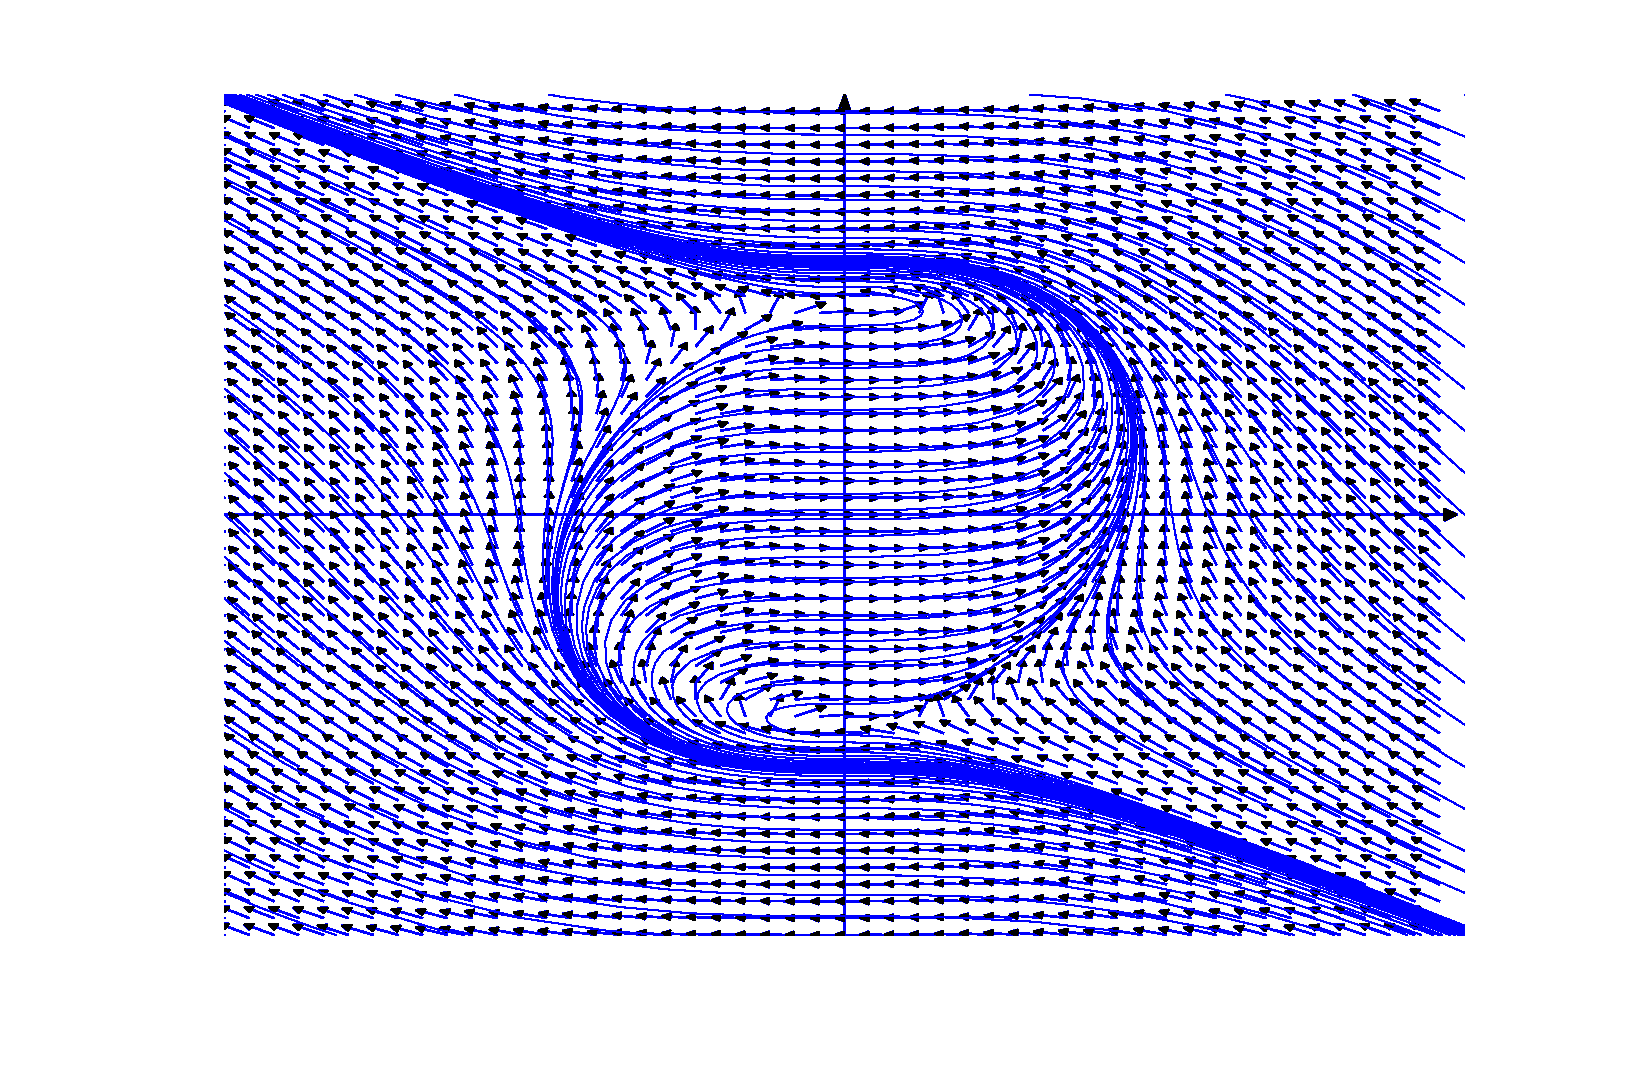
\includegraphics[bb=-78 148 689 643,width=5.67in,height=3.66in,keepaspectratio]{cover}
\end{figure}

\vspace*{.1in}
\bf\huge
\href{http://ramanujan.math.trinity.edu/wtrench/index.shtml}
{William F. Trench}
\smallskip

\large
Andrew G. Cowles Distinguished Professor Emeritus\\
Department of Mathematics\\
Trinity University \\
San Antonio, Texas, USA\\
\href{mailto:{wtrench
@trinity.edu}}
{wtrench@trinity.edu}
\large

\begin{quote}
This book has been judged to meet the evaluation criteria set by the
Editorial  Board
of the American Institute of Mathematics in connection with the Institute's
\href{http://www.aimath.org/textbooks/}
{Open
Textbook Initiative}.
It may be copied, modified, redistributed, translated,  and
built upon  subject to the  Creative Commons
\href{http://creativecommons.org/licenses/by-nc-sa/3.0/deed.en_G}
{Attribution-NonCommercial-ShareAlike 3.0 Unported
License}.
\end{quote}


\vspace{.2in}
\href{http://ramanujan.math.trinity.edu/wtrench/texts/TRENCH_DE_STUDENT_MANUAL.PDF}
{\bf FREE DOWNLOAD: STUDENT SOLUTIONS MANUAL}

\end{center}

\newpage

\vspace*{2in}

\noindent
\medskip

\noindent
Free Edition 1.01 (December 2013)

\medskip
\thispagestyle{empty}

\noindent
This book was  published previously by Brooks/Cole Thomson Learning, 2001.
This free edition is made available in the hope that it will be useful
as a textbook or reference.
 Reproduction  is
permitted
for any valid  noncommercial educational, mathematical, or scientific
purpose.
However,
charges for
profit beyond reasonable printing costs
are  prohibited.

\vspace*{.51in}


\newpage

\noindent
\thispagestyle{empty}
\vspace*{3in}
\centerline{\color{blue}\bf\Huge TO BEVERLY}

\newpage

\pagenumbering{roman}
\setcounter{page}{4}
\thispagestyle{plain}

\pdfbookmark[0]{Table of Contents}{contents}
\markboth
{\hskip1em Contents\hfill}
{\hfill }
\vspace*{3.9pc}
\centerline{\bf \Huge Contents}
\vspace*{4.8pc}
\bf
  Chapter~1 \space Introduction\hskip1em
\hfill{\color{red}1}

\vspace*{15pt}

1.1   Applications Leading to Differential Equations\hfill

1.2 \space First Order Equations\hfill\pageref{eq:1.1.9}

1.3 \space Direction Fields for First Order Equations
\hfill\pageref{eq:1.3.1}

\vspace*{15pt}

  Chapter~2 \space First Order Equations\hskip1em
\hfill\pageref{eq:2.1.1}

\vspace*{15pt}

2.1 \space Linear First Order Equations\hfill\pageref{eq:2.1.1}

2.2 \space Separable Equations \hfill\pageref{eq:2.2.1}

2.3 \space Existence and Uniqueness of Solutions of Nonlinear Equations\hfill\pageref{exer:2.2.39}

2.4 \space Transformation of Nonlinear Equations into Separable Equations\hfill\pageref{eq:2.4.1}

2.5 \space Exact Equations\hfill \pageref{eq:2.5.1}

2.6 \space  Integrating Factors \hfill \pageref{eq:2.6.1}

\vspace*{15pt}

  Chapter~3 \space Numerical Methods\hskip1em
\hfill

\vspace*{15pt}

3.1 \space Euler's Method\hfill \pageref{eq:3.1.1}

3.2 \space The Improved Euler Method and Related Methods\hfill
\pageref{eq:3.2.1}

3.3 \space The Runge-Kutta Method\hfill \pageref{eq:3.3.1}

\vspace*{15pt}

  Chapter~4 \space  Applications of First Order
Equations1em\hfill\pageref{eq:4.1.1}

\vspace*{15pt}

 4.1 \space Growth and Decay \hfill\pageref{eq:4.1.1}

 4.2 \space Cooling and Mixing\hfill \pageref{eq:4.2.1}

 4.3 \space Elementary Mechanics\hfill \pageref{eq:4.3.1}

4.4 \space Autonomous Second Order Equations\hfill \pageref{eq:4.4.1}

4.5 \space Applications to Curves\hfill \pageref{eq:4.5.1}

\vspace*{15pt}
  Chapter~5 \space Linear Second Order Equations\hskip1em
\hfill

\vspace*{15pt}

5.1 \space Homogeneous Linear Equations\hfill \pageref{eq:5.1.1}

5.2 \space Constant Coefficient Homogeneous
Equations\hfill\pageref{eq:5.2.1}

5.3 \space Nonhomgeneous Linear Equations\hfill \pageref{eq:5.3.1}

5.4 \space The Method of Undetermined Coefficients I\hfill
\pageref{eq:5.4.1}

5.5 \space The Method of Undetermined Coefficients II\hfill
\pageref{eq:5.5.1}

5.6 \space Reduction of Order\hfill \pageref{eq:5.6.1}

5.7 \space Variation of Parameters\hfill \pageref{eq:5.7.1}

\vspace*{15pt}

Chapter~6 \space   Applcations of Linear Second Order  Equations
\hfill \pageref{eq:6.1.1}

\vspace*{15pt}

6.1 \space Spring Problems I\hfill  \pageref{eq:6.1.1}

6.2 \space Spring Problems II\hfill \pageref{eq:6.2.1}

6.3 \space  The $RLC$ Circuit\hfill \pageref{eq:6.3.1}

6.4 \space Motion Under a Central Force\hfill \pageref{eq:6.4.1}

\vspace*{15pt}

  Chapter~7 \space Series Solutions of Linear Second Order Equations\hskip1em
\hfill

\vspace*{15pt}

7.1 \space Review of Power Series\hfill \pageref{thmtype:7.1.1}

7.2  \space Series Solutions Near an Ordinary Point I\space
\hfill\pageref{eq:7.2.1}

7.3  \space Series Solutions Near an Ordinary Point II\space \hfill
\pageref{eq:7.3.1}

7.4 \space Regular Singular Points   Euler Equations\hfill
\pageref{eq:7.4.1}

7.5 \space The Method of Frobenius I\space \hfill \pageref{eq:7.5.1}

7.6 \space The Method of Frobenius II\space \hfill \pageref{eq:7.6.1}

7.7 \space The Method of Frobenius III \hfill \pageref{eq:7.7.1}

\vspace*{15pt}

Chapter~8 \space Laplace Transforms\hskip1em
\hfill

\vspace*{15pt}

8.1 \space Introduction to the Laplace Transform\hfill \pageref{eq:8.1.1}

8.2 \space The Inverse Laplace Transform\hfill\pageref{example:8.2.1}

8.3 \space Solution of Initial Value Problems\hfill \pageref{thmtype:8.3.1}

8.4 \space The Unit Step Function\hfill \pageref{example:8.4.1}

8.5 \space Constant Coefficient Equations with Piecewise Continuous
 Forcing\\ \hspace*{.24in}Functions\hfill\pageref{eq:8.5.1}

8.6 \space Convolution\hfill \pageref{eq:8.6.2}

8.7 \space Constant Cofficient Equations with Impulses\hfill
\pageref{exer:8.6.14}

8.8 \space A Brief Table of Laplace Transforms\hfill

\thispagestyle{empty}
\vspace*{15pt}

  Chapter~9 \space Linear Higher Order Equations\hskip1em
\hfill

\vspace*{15pt}

9.1 \space Introduction to Linear Higher Order Equations\hfill
\pageref{eq:9.1.1}

9.2 \space Higher Order Constant Coefficient Homogeneous Equations\hfill
\pageref{eq:9.2.1}

9.3 \space Undetermined Coefficients for Higher Order Equations\hfill
\pageref{eq:9.3.1}

9.4 \space Variation of Parameters for Higher Order Equations\hfill
\pageref{eq:9.4.1}

\vspace*{15pt}

  Chapter~10 \space  Linear Systems of Differential Equations\hskip1em

\vspace*{15pt}

10.1 \space Introduction to Systems of Differential Equations\hfill
\pageref{example:10.1.1}

10.2 \space Linear Systems of Differential Equations\hfill
\pageref{eq:10.2.1}

10.3 \space  Basic Theory of Homogeneous Linear Systems\hfill
\pageref{eq:10.3.1}

10.4 \space Constant Coefficient Homogeneous Systems I\hfill
\pageref{eq:10.4.1}

10.5 \space Constant Coefficient Homogeneous Systems II\hfill
\pageref{example:10.5.1}

10.6 \space Constant Coefficient Homogeneous Systems II\hfill
\pageref{eq:10.6.1}

10.7 \space  Variation of Parameters for Nonhomogeneous Linear Systems\hfill \pageref{thmtype:10.7.1}

\vspace*{15pt}

  Chapter~11 \space Boundary Value Problems and Fourier Expansions\hskip1em
\hfill \pageref{thmtype:11.1.1}

\vspace*{15pt}

11.1 \space Eigenvalue Problems for ${\mathbf y''+\lambda y=0}$\hfill
\pageref{thmtype:11.1.1}

11.2 \space Fourier Series I\hfill \pageref{thmtype:11.2.1}

11.3 \space Fourier Series II\hfill \pageref{eq:11.3.1}

\vspace*{15pt}

  Chapter~12 \space Fourier  Solutions of Partial Differential
Equations\hskip1em
\hfill

\vspace*{15pt}

12.1 \space The Heat Equation\hfill \pageref{eq:12.1.1}

12.2 \space The Wave Equation\hfill \pageref{eq:12.2.1}

12.3 \space Laplace's Equation in Rectangular Coordinates\hfill
\pageref{eq:12.3.1}

12.4 \space Laplace's Equation in Polar Coordinates\hfill
\pageref{eq:12.4.1}

\vspace*{15pt}

  Chapter~13 \space Boundary Value Problems for Second Order Linear
Equations\hskip1em
\hfill

\vspace*{15pt}

13.1 \space Boundary Value Problems\hfill \pageref{eq:13.1.1}

13.2 \space Sturm--Liouville Problems\hfill \pageref{eq:13.2.1}

\rm

\newpage

\setlength{\parindent}{10pt}

\pdfbookmark[0]{Preface}{preface}
\markboth
{\hskip1em Preface\hfill}
{\hfill Preface\hskip1em}
\thispagestyle{plain}
\vspace*{3.9pc}
\centerline{\bf \Huge Preface}
\bigskip

\noindent
{\color{blue}\it Elementary Differential Equations with Boundary Value Problems\/}
 is
written for students in science, engineering, and mathematics who have
completed calculus  through partial  differentiation. If  your syllabus
includes Chapter~10 (Linear  Systems of Differential  Equations),
your students should have some preparation in linear algebra.

In writing this book I have been guided by the these principles:

\begin{itemize}

\item An elementary text should be written so  the student can
read it with comprehension without too much pain. I have tried to
put myself in the student's place, and have chosen to err on the side
of too much detail rather than not enough.

\item An elementary text can't be better than its exercises.
This text includes  2041 numbered exercises, many with several parts.
They range in difficulty from routine to very challenging.

\item An elementary text should be written in an informal but
mathematically accurate way, illustrated by appropriate graphics.
I have tried to formulate
mathematical concepts succinctly
 in language that students can understand. I have
minimized the number of explicitly stated theorems and definitions,
preferring to deal with concepts in a more conversational way,
copiously illustrated by 299 completely worked out examples. Where
appropriate, concepts and results are depicted in 188 figures.
\end{itemize}

%###
Although I believe that the computer is an immensely valuable tool for
learning, doing, and writing mathematics, the selection and treatment
of topics in this text reflects my pedagogical orientation along
traditional lines. However, I have incorporated what I believe to be
the best use of modern technology, so you can select the level of
technology that you want to include in your course. The text includes
414 exercises -- identified by the symbols \Cex  and \CGex -- that call
for graphics or computation and graphics. There are also
79 laboratory exercises -- identified by \Lex -- that require extensive
use of technology. In addition, several sections include informal advice on
the use of technology. If you prefer not to emphasize technology,
simply ignore these exercises and the  advice.

There are two schools of thought on whether techniques and
applications should be treated together or separately. I have chosen
to separate them;   thus, Chapter~2 deals with techniques for solving
first order equations, and Chapter~4 deals with applications.
Similarly, Chapter~5 deals with techniques for solving second order
equations, and Chapter~6 deals with applications. However, the
exercise sets of the sections dealing with techniques  include some
applied problems.

Traditionally oriented elementary differential
equations texts are occasionally  criticized as being collections of
unrelated methods for solving miscellaneous problems. To some extent
this is true;     after all, no single method  applies to all
situations. Nevertheless, I believe that one idea can go a long way
toward unifying some of the techniques for solving diverse problems:
variation of parameters. I use variation of parameters at the earliest
opportunity in Section~2.1, to solve the nonhomogeneous linear
equation, given a nontrivial solution of the complementary equation.
You may find this annoying, since most of us learned that one should
use integrating factors for this task, while perhaps mentioning the
variation of parameters option in an exercise. However, there's
little difference between the two approaches, since an integrating
factor is nothing more than the reciprocal of a nontrivial solution of
the complementary equation. The advantage of using variation of
parameters here is that it introduces the concept in its simplest form
and focuses the student's attention on the idea of seeking a solution
$y$ of a differential equation by writing it as $y=uy_1$, where $y_1$
is a known solution of related equation and $u$ is a function to be
determined. I use this idea in nonstandard ways, as follows:

\begin{itemize}
\item
In Section~2.4 to solve nonlinear first order equations, such as
Bernoulli equations and nonlinear homogeneous equations.

\item  In Chapter~3  for  numerical solution of
semilinear  first order equations.

\item In Section 5.2 to avoid the necessity of introducing complex
exponentials in solving a second order constant coefficient
homogeneous equation with characteristic polynomials  that have complex
zeros.

\item In Sections~5.4, 5.5, and 9.3 for the method of undetermined
coefficients. (If the method of annihilators is your preferred
approach to this problem, compare the labor involved in solving, for
example, $y''+y'+y=x^4e^x$ by the method of annihilators and the
method used in Section~5.4.)
\end{itemize}

Introducing variation of parameters as early as possible (Section~2.1)
prepares the student for the concept when it appears again in more
complex forms in Section~5.6, where reduction of order is used not
merely to find a second solution of the complementary equation, but
also to find the general solution of the nonhomogeneous equation, and
in Sections~5.7, 9.4, and 10.7, that treat the usual variation of
parameters problem for second and higher order linear equations and
for linear systems.

Chapter~11 develops the theory of Fourier series.
 Section~11.1 discusses the five main eigenvalue problems
that arise in connection with the method of separation of
variables for the heat and wave equations and for Laplace's
equation over a rectangular domain:

 Problem 1: \hskip5em  $y''+\lambda y=0,\quad y(0)=0,\quad y(L)=0$
\medskip

  Problem 2:  \hskip5em $y''+\lambda y=0,\quad y'(0)=0,\quad y'(L)=0$
\medskip

 Problem 3: \hskip5em $y''+\lambda y=0,\quad y(0)=0,\quad y'(L)=0$
\medskip

  Problem 4: \hskip5em $y''+\lambda y=0,\quad y'(0)=0,\quad y(L)=0$
\medskip

 Problem 5: \hskip5em $y''+\lambda y=0,\quad y(-L)=y(L),
\quad y'(-L)=y'(L)$
\medskip

 These problems are handled in a
unified way     for example, a single theorem shows that the
eigenvalues of all five problems are nonnegative.

Section~11.2 presents the  Fourier series expansion
of functions defined on
on $[-L,L]$,   interpreting it as an expansion in terms of the
eigenfunctions of Problem~5.

 Section~11.3  presents the
 Fourier sine and cosine expansions of functions defined on
$[0,L]$, interpreting them as expansions in terms of the
eigenfunctions of Problems~1 and 2, respectively. In addition,
Section~11.2 includes what I call the mixed Fourier sine and
cosine expansions, in terms of the eigenfunctions of Problems~4
and 5, respectively. In all cases, the convergence properties of
these series are deduced from the convergence properties of
the Fourier series discussed in Section~11.1.

Chapter~12 consists of four sections devoted to the
heat equation, the wave equation, and Laplace's equation
in rectangular and polar coordinates.
For all three, I consider homogeneous boundary conditions
of the four types occurring in Problems~1-4. I present
the method of separation of variables as a way of
choosing the appropriate form for the series expansion
of the solution of the given problem, stating---without
belaboring the point---that the expansion may fall short of being
an actual solution, and giving an indication of conditions under
which the formal solution is an actual solution. In particular, I
found it necessary
to devote some detail to this question  in connection with the wave
equation in Section~12.2.

In Sections~12.1 (The Heat Equation) and 12.2 (The Wave Equation) I
devote considerable effort to devising examples and numerous
exercises where the functions defining the initial conditions
satisfy
the homogeneous boundary conditions. Similarly, in most of the
examples and exercises Section~12.3
(Laplace's Equation), the functions defining the boundary conditions
on a given side of the rectangular domain satisfy homogeneous
boundary conditions at the endpoints of the same type (Dirichlet or
Neumann) as the boundary conditions imposed on adjacent sides of
the region. Therefore  the formal solutions obtained in many of the
examples and exercises are  actual solutions.

Section~13.1  deals with two-point value problems for
a second order ordinary differential equation. Conditions for
existence
and uniqueness of solutions are given, and the construction
of Green's functions is included.

Section~13.2  presents the elementary aspects of Sturm-Liouville
theory.

You may also find the following to be of interest:

\begin{itemize}

\item Section~2.6 deals with integrating factors of the form
$\mu=p(x)q(y)$, in addition to those of the form $\mu=p(x)$ and
$\mu=q(y)$ discussed in most texts.

\item
Section~4.4 makes phase plane analysis of nonlinear second order
autonomous equations accessible to students who have not taken linear
algebra, since eigenvalues and eigenvectors do not enter into the
treatment. Phase plane analysis of constant coefficient linear systems
is included in Sections~10.4-6.

\item Section~4.5 presents an extensive discussion of applications
of differential equations to curves.

\item Section~6.4 studies motion under a central force,
which may be useful to students interested in the mathematics of
satellite orbits.

\item Sections~7.5-7 present the method of Frobenius in more detail
than  in most texts. The approach is to systematize the
computations in a way that avoids the necessity of substituting the
unknown Frobenius series into each equation. This leads to efficiency
in the computation of the coefficients of the Frobenius solution. It
also clarifies the case where the roots of the indicial equation
differ by an integer (Section~7.7).

\item The free Student Solutions Manual contains solutions
of most of the even-numbered exercises.

 \item The free  Instructor's Solutions Manual is available by email to
\href{mailto:wtrench@trinity.edu}
{wtrench@trinity.edu},
 subject to verification of the requestor's
faculty status.

\end{itemize}

The following observations may be helpful as you choose your
 syllabus:

\begin{itemize}
\item Section~2.3  is the only specific prerequisite for Chapter~3.
To accomodate institutions that offer a separate course
in numerical analysis,  Chapter~3 is not
a prerequisite for any other section in the text.

\item The sections in Chapter~4 are  independent of each
other, and  are not prerequisites for any of the later chapters. This
is also true of the sections in Chapter~6, except that Section~6.1
is a prerequisite for Section~6.2.

\item Chapters~7, 8, and 9 can be covered in any order after
the topics selected  from Chapter~5. For example, you can
proceed directly from Chapter~5 to Chapter~9.

\item The second order Euler equation is discussed in Section~7.4,
where it sets the stage for the method of Frobenius. As noted at the
beginning of Section~7.4, if you want to include Euler equations in
your syllabus while omitting the method of Frobenius, you can skip the
introductory paragraphs in Section~7.4 and begin with
Definition~7.4.2. You can then cover
Section~7.4 immediately after  Section~5.2.

\enlargethispage{1in}
\item Chapters~11, 12, and 13 can be covered at any time
after the completion of Chapter~5.

\end{itemize}

\par\medskip
\noindent\mbox{\hspace*{275pt}}William F. Trench\mbox{}

\newpage
\setcounter{page}{1}
\pagenumbering{arabic}
\thispagestyle{plain}

\setcounter{chapter}{1}
\pdfbookmark[0]{Chapter 1 Introduction}{chapter:1}
\chaptertitle{Introduction}

\noindent
IN THIS CHAPTER we begin our study of differential equations.

\medskip\noindent
 SECTION~1.1 presents
examples of applications that lead to differential equations.

\medskip\noindent
SECTION~1.2 introduces   basic concepts and
definitions concerning differential equations.

\medskip\noindent
 SECTION~1.3
presents a geometric method for dealing with differential equations
that has been known for a very long time, but has become particularly
useful and important with the proliferation of readily available
differential equations software.

\newpage

\newsection{1}{Introduction} { Applications Leading to Differential Equations}
\subpdfbookmark{Section 1.1 Some Applications Leading to Differential Equations} {section:1.1}
\vskip14pt
\setcounter{section}{1}
\newcommand{\thissection}
{\sectiontitle{ APPLICATIONS LEADING TO DIFFERENTIAL EQUATIONS\,}}
\thissection

\noindent
In order to apply mathematical methods to a physical or ``real life''
problem, we must  formulate the problem in mathematical
terms; that is, we must construct a {\color{blue}\it mathematical
model\/} for the
problem. Many physical problems concern relationships between changing
quantities. Since rates of change are represented mathematically by
derivatives, mathematical models often involve equations relating an
unknown function and one or more of its derivatives. Such equations
are  {\color{blue}\it differential equations}. They are the subject of this
book.

Much of calculus is devoted to learning mathematical techniques that
are applied in later courses in mathematics and the sciences;     you
wouldn't have time to learn much calculus if you insisted on seeing
a specific application of every topic covered in the course.
Similarly, much of this book is devoted to methods that can be applied
in later courses. Only a relatively small part of the book is devoted
to the derivation of specific differential equations from mathematical
models, or relating the differential equations that we study to
specific applications. In this section we mention a few such
applications.

The mathematical model for an applied problem is almost always simpler
than the actual situation being studied, since simplifying assumptions
are usually required to obtain a mathematical problem that can be
solved. For example, in modeling the motion of a falling object, we
might neglect air resistance and the gravitational pull of celestial
bodies other than Earth, or in  modeling  population growth we
might assume that the population grows continuously rather than in
discrete steps.

A good mathematical model has two important properties:

\begin{itemize}
\item It's sufficiently simple so that the mathematical problem
can be solved.

\item It represents the actual situation sufficiently well so that the
solution to the mathematical problem predicts the outcome of the real
problem to within a useful degree of accuracy. If results predicted by
the model don't agree with physical observations, the
underlying
assumptions of the model must be revised until satisfactory agreement
is obtained.
\end{itemize}

We'll  now give  examples of mathematical models involving
differential equations. We'll return to these problems at the
appropriate times, as we learn how to solve the various types of
differential equations that occur in the models.

All the examples in this section deal with functions of time, which we
 denote by $t$. If $y$ is a function of $t$,  $y'$
denotes the derivative of $y$ with respect to $t$;   thus,
$$
y'={dy\over dt}.
$$

\boxit{Population Growth and Decay}

\noindent
Although the number of members of a population (people in a given
country, bacteria in a laboratory culture, wildflowers in a forest,
etc.)
at any given time $t$ is necessarily an integer, models that use
differential equations to describe the growth and decay of populations
usually rest on the simplifying assumption that the number of members of
the population can be regarded as a differentiable function $P=P(t)$.
In most models it is assumed that the differential equation takes the
form
\begin{equation} \label{eq:1.1.1}
P'=a(P)P,
\end{equation}
where $a$ is a continuous function of $P$ that represents the rate of
change of population per unit time per individual.
In the
\href{http://en.wikipedia.org/wiki/Thomas_Robert_Malthus}
{\color{blue}\it Malthusian model},
 it is assumed that
$a(P)$ is a constant, so \eqref{eq:1.1.1} becomes
\begin{equation} \label{eq:1.1.2}
P'=aP.
\end{equation}
\color{blue}
(When you see a name in blue italics, just click on it for
information about the person.)
\color{black}
This model assumes that the numbers of births and deaths per unit time
are both proportional to the population. The constants of
proportionality are  the {\color{blue}\it birth rate\/} (births per unit
time per individual) and the {\color{blue}\it death rate\/} (deaths per unit time
per individual);     $a$ is the birth rate minus the death rate.
You  learned in calculus that if $c$ is any constant then
\begin{equation} \label{eq:1.1.3}
P=ce^{at}
\end{equation}
satisfies \eqref{eq:1.1.2}, so \eqref{eq:1.1.2} has infinitely
many solutions. To select the solution of the specific problem that
we're considering, we must know the population $P_0$ at an initial
time, say $t=0$. Setting $t=0$ in \eqref{eq:1.1.3} yields
$c=P(0)=P_0$, so the applicable solution is
$$
P(t)=P_0e^{at}.
$$
This implies that
$$
\lim_{t\to\infty}P(t)=\left\{\begin{array}{cl}\infty&\mbox{ if
}a>0,\\ 0&\mbox{ if }a<0;    \end{array}\right.
$$
that is, the population approaches infinity if the birth rate exceeds
the death rate, or zero if the death rate exceeds the birth rate.

To see the limitations of the Malthusian model, suppose  we're
modeling the  population of a country, starting from a time
$t=0$ when the birth rate exceeds the death rate (so $a>0$), and
the country's resources in terms of space, food supply, and other
necessities of life can support the existing population. Then the
prediction $P=P_0e^{at}$ may be reasonably accurate as long as
it remains within limits that the country's resources can support.
However, the model must inevitably lose validity when the prediction
exceeds these limits. (If nothing else, eventually there won't be
enough space for the predicted population!)

This flaw in the Malthusian model suggests the need for a model that
accounts for limitations of space and resources that tend to oppose
the rate of population growth as the population increases.
 Perhaps the most famous model of this kind is the
\href{http://www-history.mcs.st-and.ac.uk/Mathematicians/Verhulst.html}
{\color{blue}\it Verhulst
 model\/}, where \eqref{eq:1.1.2} is
replaced by
\begin{equation} \label{eq:1.1.4}
P'=aP(1-\alpha P),
\end{equation}
where $\alpha$ is a positive constant.
As long as $P$ is small
compared to $1/\alpha$, the ratio $P'/P$  is approximately equal to $a$.
Therefore the growth is approximately exponential;     however, as $P$
increases, the ratio $P'/P$  decreases as opposing factors
become significant.

Equation~\eqref{eq:1.1.4} is  the {\color{blue}\it logistic equation\/}. You
will learn how to solve it in Section~1.2. (See
Exercise~2.2.~\hspace*{-3pt}\ref{exer:2.2.28}.) The solution is
$$
P={P_0\over\alpha P_0+(1-\alpha P_0)e^{-at}},
$$
where $P_0=P(0)>0$. Therefore
$\lim_{t\to\infty}P(t)=1/\alpha$, independent of $P_0$.

Figure~\ref{figure:1.1.1} shows typical graphs of $P$ versus $t$ for
various values of  $P_0$.

\begin{figure}[h]
  \centering
  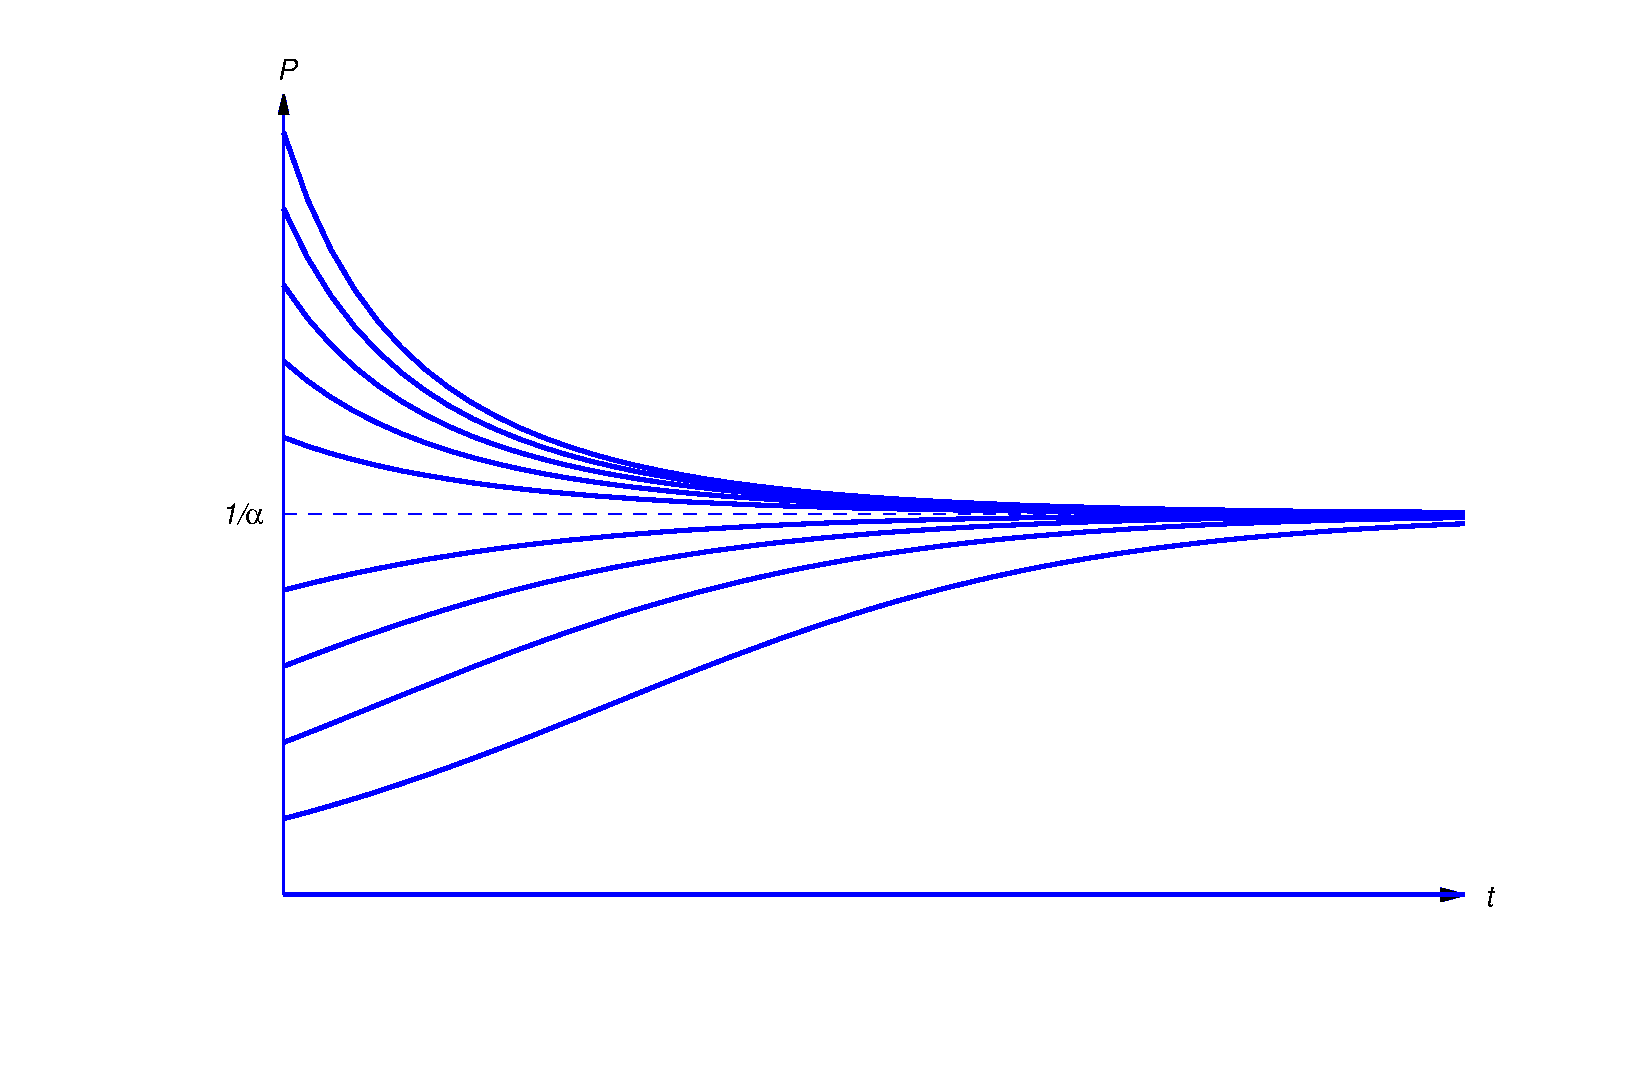
\includegraphics[bb=-78 148 689 643,width=5.67in,height=3.66in,keepaspectratio]{fig010101}
\color{blue}
  \caption{ Solutions of the logistic equation}
  \label{figure:1.1.1}
\end{figure}


\boxit{Newton's Law of Cooling}

\noindent
According to
\href{http://www-history.mcs.st-and.ac.uk/Mathematicians/Newton.html}
{\color{blue}\it Newton's
law of cooling},  the temperature of a
body changes at a rate proportional to the difference between the
temperature of the body and the temperature of the surrounding medium.
 Thus, if  $T_m$ is the temperature of the
medium and
$T=T(t)$ is the temperature of the body at time $t$, then
\begin{equation} \label{eq:1.1.5}
T' = -k(T-T_m),
\end{equation}
where $k$ is a positive constant and the  minus sign indicates;   that
the temperature of the body increases with time if it's less than the
temperature of the medium, or decreases if it's  greater. We'll see
in Section~4.2 that if
$T_m$ is constant then the solution of \eqref{eq:1.1.5} is
\begin{equation} \label{eq:1.1.6}
T=T_m+(T_0-T_m)e^{-kt},
\end{equation}
where $T_0$ is the temperature of the body when $t=0$.
Therefore $\lim_{t\to\infty}T(t)=T_m$, independent of $T_0$.
(Common sense suggests this. Why?)

Figure~\ref{figure:1.1.2} shows typical graphs of $T$ versus $t$ for
various values of  $T_0$.

\begin{figure}[htp]
  \centering
  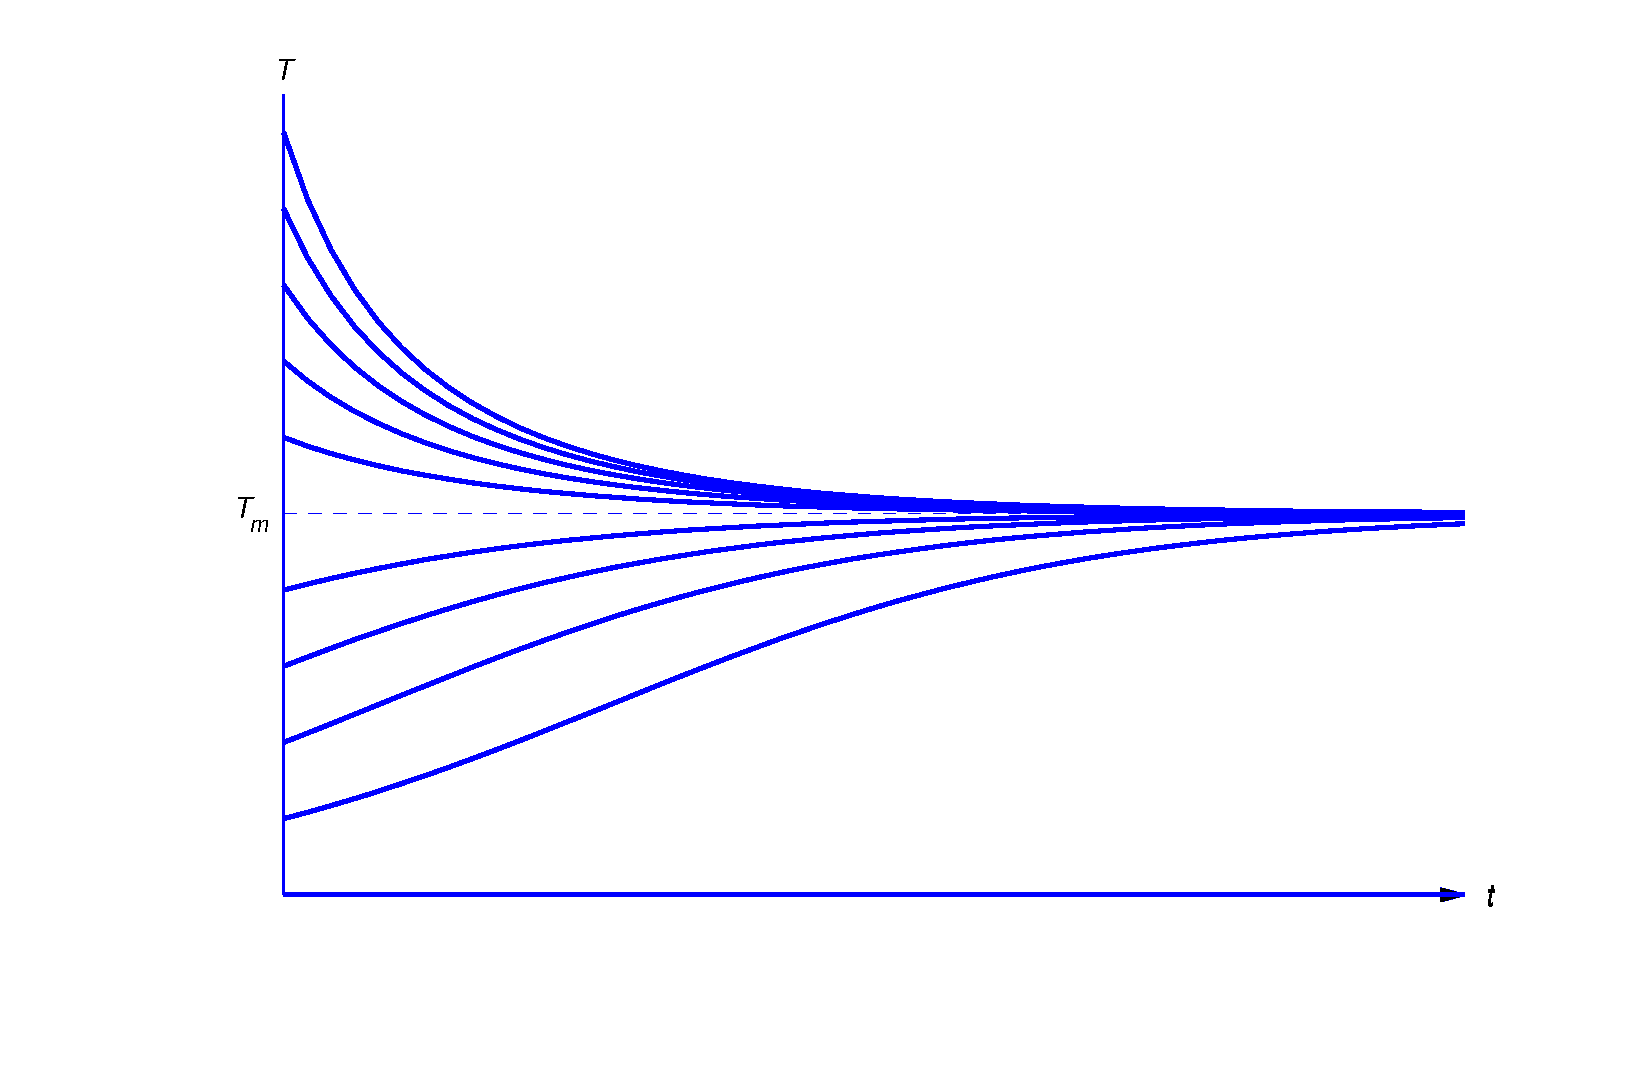
\includegraphics[bb=-78 148 689 643,width=5.67in,height=3.66in,keepaspectratio]{fig010102}
\color{blue}
  \caption{ Temperature according to Newton's Law of Cooling}
  \label{figure:1.1.2}
\end{figure}

Assuming that the medium remains at constant temperature seems
reasonable if we're considering a cup of coffee cooling in a room, but
 not if we're cooling a huge cauldron of molten
metal in the same room. The difference between the two situations is
that the heat lost by the coffee isn't likely to raise the
temperature of the room appreciably, but the heat lost by the
cooling metal is. In this second situation we must use a model that
accounts for the heat exchanged between the object and the medium. Let
$T=T(t)$ and $T_m=T_m(t)$ be the temperatures of the object and the
medium respectively, and let $T_0$ and $T_{m0}$ be their initial
values. Again, we assume that $T$ and $T_m$ are related by
\eqref{eq:1.1.5}. We also assume that the change in heat of
the object as its temperature changes from $T_0$ to $T$ is $a(T-T_0)$
and  the change in heat of the medium as its temperature changes
from $T_{m0}$ to $T_m$ is $a_m(T_m-T_{m0})$, where $a$ and $a_m$ are
positive constants depending upon the masses and thermal properties of
the object and medium respectively. If we assume that the total heat
of the in the object and the medium remains constant
(that is, energy is conserved), then
$$
a(T-T_0)+a_m(T_m-T_{m0})=0.
$$
Solving this for  $T_m$  and substituting the result into
\eqref{eq:1.1.6} yields the differential equation
$$
T'=-k\left(1+{a\over a_m}\right)T
+k\left(T_{m0}+{a\over a_m}T_0\right)
$$
for the temperature of the object.  After learning to solve linear
first order  equations, you'll be able to show
(Exercise~4.2.~\hspace*{-3pt}\ref{exer:4.2.17}) that
$$
T={aT_0+a_mT_{m0}\over
a+a_m}+{a_m(T_0-T_{m0})\over a+a_m}e^{-k(1+a/a_m)t}.
$$

\boxit{Glucose Absorption by the Body}

\noindent
Glucose is absorbed by
the body at a rate proportional to the amount of glucose present in
the bloodstream. Let $\lambda$ denote the (positive) constant of
proportionality. Suppose   there are $G_0$ units of glucose in
the bloodstream when $t=0$, and let $G=G(t)$ be the number of units in
the bloodstream at time $t>0$. Then, since the glucose being absorbed
by the body is leaving the bloodstream, $G$ satisfies the equation
\begin{equation} \label{eq:1.1.7}
G'=-\lambda G.
\end{equation}
From  calculus you know that if $c$ is any constant then
\begin{equation} \label{eq:1.1.8}
G=ce^{-\lambda t}
\end{equation}
satisfies \eqref{eq:1.1.7}, so \eqref{eq:1.1.7} has infinitely
many solutions.
 Setting $t=0$ in \eqref{eq:1.1.8} and requiring that
$G(0)=G_0$ yields $c=G_0$, so
$$
G(t)=G_0e^{-\lambda t}.
$$

Now let's complicate matters by injecting glucose intravenously
at a constant rate of $r$ units of glucose per unit of time.
Then the rate of change of the amount of glucose  in the bloodstream
per unit time is
\begin{equation} \label{eq:1.1.9}
G'=-\lambda G+r,
\end{equation}
where the first term on the right is due to the absorption of the
glucose by the body and the second term is due to the injection.
 After you've studied Section~2.1,
you'll be able to show (Exercise~2.1.~\hspace*{-3pt}\ref{exer:2.1.43}) that the solution
of
\eqref{eq:1.1.9} that satisfies $G(0)=G_0$ is
$$
G={r\over\lambda}+\left(G_0-{r\over\lambda}\right)e^{-\lambda t}.
$$
Graphs of  this function are similar to those in
Figure~\ref{figure:1.1.2}.
(Why?)

\boxit{Spread of Epidemics}

\noindent
One model for the spread of epidemics assumes that the number of
people infected changes at a rate proportional to the product of the
number of people already infected and the number of people who are
susceptible, but not yet infected. Therefore, if $S$ denotes the
total population of susceptible people and $I=I(t)$ denotes the
number
of infected people at time $t$, then $S-I$ is the number of people
who are susceptible, but not yet infected. Thus,
$$
I'=rI(S-I),
$$
where $r$ is a positive constant. Assuming that $I(0)=I_0$,
the solution of this equation is
$$
I={SI_0\over I_0+(S-I_0)e^{-rSt}}
$$
(Exercise~2.2.~\hspace*{-3pt}\ref{exer:2.2.29}).
 Graphs of this function are similar to those in
Figure~\ref{figure:1.1.1}.
(Why?)
Since $\lim_{t\to\infty}I(t)=S$, this model predicts that all the
susceptible people eventually become infected.

\boxit{Newton's Second Law of Motion}

\noindent

According to
\href{http://www-history.mcs.st-and.ac.uk/Mathematicians/Newton.html}
{\color{blue}\it Newton's second law of motion},  the
instantaneous acceleration
$a$ of an object with constant mass $m$ is related to the force $F$
acting on the object by the equation $F=ma$. For simplicity, let's
assume that $m=1$ and the motion of the object is along a vertical
line. Let $y$ be the displacement of the object from some reference
point on Earth's surface, measured positive upward. In many
applications, there are three kinds of forces that may act on the
object:

\begin{alist}
\item % (a)
A force such as gravity that depends only on the position $y$,
which we write as $-p(y)$, where $p(y)>0$ if $y\ge0$.

\item % (b)
A force such as atmospheric resistance that depends on
the position and velocity of the object, which we write as
$-q(y,y')y'$, where $q$ is a nonnegative function and we've
put $y'$ ``outside'' to indicate that the resistive force is
always in the direction opposite to the velocity.
\item % (c)
A force $f=f(t)$, exerted from an external source (such as a towline
from a helicopter) that depends only on $t$.
\end{alist}

In this case, Newton's second law implies that
$$
y''=-q(y,y')y'-p(y)+f(t),
$$
which is usually rewritten as
$$
y''+q(y,y')y'+p(y)=f(t).
$$
Since the  second (and no higher) order derivative of $y$ occurs in
this equation, we say that it is a {\color{blue}\it second order differential
equation\/}.

\boxit{Interacting Species: Competition}

\noindent
Let $P=P(t)$ and $Q=Q(t)$ be the populations of two species at time
$t$, and assume that each population would grow exponentially if the
other didn't exist; that is, in the absence of competition we would
have
\begin{equation} \label{eq:1.1.10}
P'=aP \mbox{\quad and \quad}Q'=bQ,
\end{equation}
where $a$ and $b$ are positive constants. One way to model the effect
of competition is to assume that the growth rate per individual of
each population is reduced by an amount proportional to the other
population, so \eqref{eq:1.1.10} is replaced by
\begin{eqnarray*}
P'&=&\phantom{-}aP-\alpha Q\\
Q'&=&-\beta P+bQ,
\end{eqnarray*}
where $\alpha$ and $\beta$ are positive constants. (Since negative
population doesn't make sense, this system works only while $P$ and
$Q$ are both positive.) Now suppose   $P(0)=P_0>0$ and
$Q(0)=Q_0>0$. It can be shown (Exercise~10.4.~\hspace*{-3pt}\ref{exer:10.4.42})
that there's a  positive constant $\rho$ such that if
$(P_0,Q_0)$ is above the line $L$ through the origin with slope $\rho$,
then the species with population $P$ becomes extinct in finite time,
but if $(P_0,Q_0)$ is below $L$,   the species with population
$Q$ becomes extinct in finite time. Figure~\ref{figure:1.1.3} illustrates
this. The curves shown there are given parametrically by $P=P(t),
Q=Q(t),\ t>0$.
 The arrows indicate direction along the curves with
increasing $t$.

\begin{figure}[h]
  \centering
  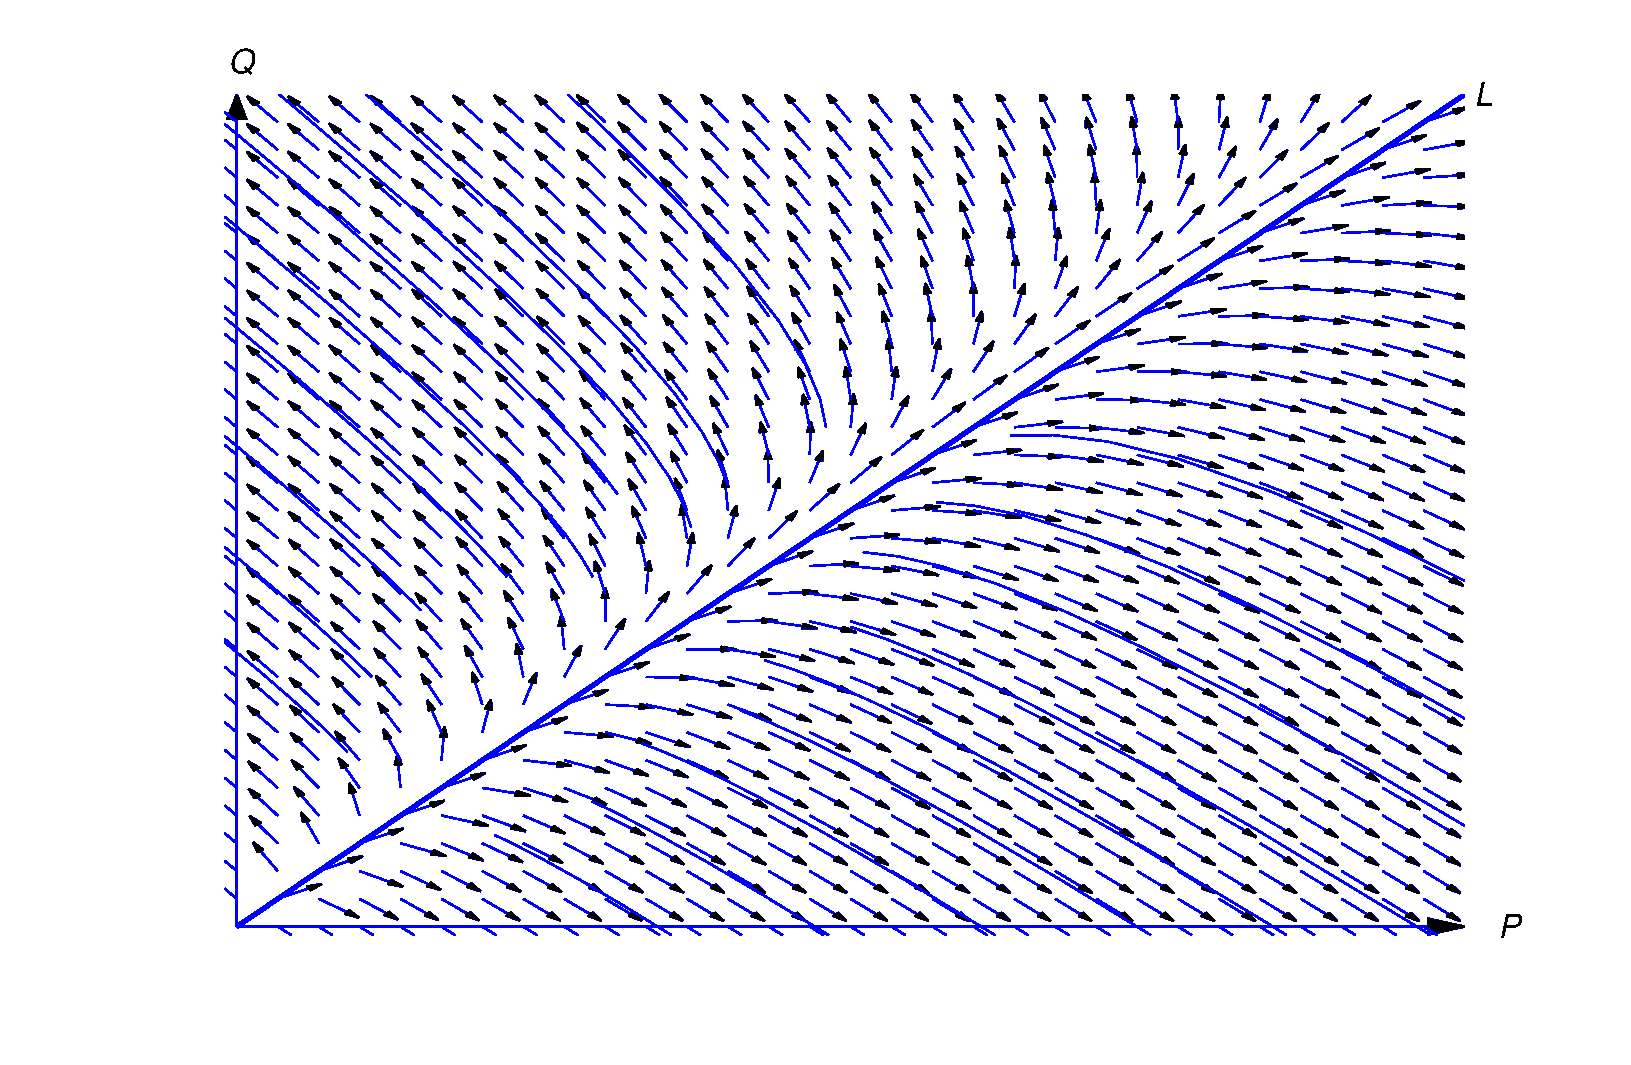
\includegraphics[bb=-78 148 689 643,width=5.67in,height=3.66in,keepaspectratio]{fig010103}
\color{blue}
  \caption{ Populations of competing species}
  \label{figure:1.1.3}
\end{figure}

\newsection{2}{Introduction} {Basic Concepts}
\currentpdfbookmark{Section 1.2 Basic Concepts}{section:1.2}
\vskip14pt
\renewcommand{\thissection}{\sectiontitle{\, BASIC CONCEPTS}}
\thissection

\noindent
A {\color{blue}\it differential equation} is an equation that contains one or more
derivatives of an unknown function. The {\color{blue}\it order\/} of a
differential equation is the order of the highest
derivative that it contains. A differential equation is an
{\color{blue}\it ordinary differential equation\/} if it involves an unknown
function of only one variable, or a {\color{blue}\it partial differential
equation\/} if it involves partial derivatives of a function of more
than one variable. For now we'll consider only ordinary differential
equations, and we'll just call them {\color{blue}\it differential equations.\/}

Throughout this text, all variables and constants are real unless it's
stated otherwise. We'll usually use $x$ for the independent variable
unless the independent variable is time; then we'll use $t$.

The simplest differential equations are first order equations of the
form
$$
{dy\over dx}=f(x) \mbox{\quad or, equivalently, \quad}y'=f(x),
$$
where $f$  is a known function of $x$. We already know from calculus
how to find functions that satisfy this kind of equation. For example,
if
$$
y'=x^3,
$$
then
$$
y=\int x^3\, dx={x^4\over4}+c,
$$
 where $c$ is an arbitrary constant.  If $n>1$
we can find functions $y$ that satisfy
equations of the form
\begin{equation} \label{eq:1.2.1}
y^{(n)}=f(x)
\end{equation}
by repeated integration. Again, this is a calculus problem.

Except for illustrative purposes in this section, there's no need to
consider differential equations like \eqref{eq:1.2.1}.We'll
usually consider differential equations that can be written as
\begin{equation} \label{eq:1.2.2}
y^{(n)}=f(x,y,y', \dots,y^{(n-1)}),
\end{equation}
where at least one of the functions $y$, $y'$, \dots, $y^{(n-1)}$ actually
appears on the right. Here are some examples:
$$
\begin{array}{rcll}
\dst{dy\over dx}-x^2&=&0&\mbox{ (first order)},  \\[2\jot]
\dst{dy\over dx}+2xy^2&=&-2&\mbox{ (first order)},   \\[2\jot]
\dst{d^2y\over dx^2}+2\dst{dy\over dx}+y&=&2x&\mbox{ (second order)},
\\[2\jot]
xy'''+y^2&=&\sin x  &\mbox{ (third order)},
\\[2\jot] y^{(n)}+xy'+3y&=&x&\mbox{ ($n$-th order)}.
\end{array}
$$
Although none of these equations is  written as in
\eqref{eq:1.2.2}, all of them {\color{blue}\it can\/} be written in this form:
$$
\begin{array}{rcl}
y'&=&x^2,  \\
y'&=&-2-2xy^2,   \\
y''&=&2x-2y'-y,  \\
y'''&=&\dst{\sin x-y^2\over x},
\\[2\jot] y^{(n)}&=&x-xy'-3y.
\end{array}
$$

\boxit{Solutions of Differential Equations}

\noindent
A {\color{blue}\it solution\/} of a differential equation is a function that
satisfies the differential equation on some open interval;   thus, $y$
is a solution of \eqref{eq:1.2.2} if $y$ is $n$ times differentiable and
$$
y^{(n)}(x)=f(x,y(x),y'(x), \dots,y^{(n-1)}(x))
$$
for all $x$ in some open interval $(a,b)$. In this case, we also say
that $y$ {\color{blue}\it is a solution of $\eqref{eq:1.2.2}$ on\/} $(a,b)$. Functions
that satisfy a differential equation at isolated points are not
interesting. For example, $y=x^2$ satisfies
$$
xy'+x^2=3x
$$
if and only if $x=0$ or $x=1$, but it's not a solution of this
differential equation because it does not satisfy the equation on an
open interval.

The graph of a solution of a differential equation is  a {\color{blue}\it
solution curve\/}. More generally, a curve $C$ is said to be an {\color{blue}\it
integral curve\/} of a differential equation if every function
$y=y(x)$ whose graph is a segment of $C$ is a solution of the
differential equation. Thus, any solution curve of a differential
equation is an integral curve, but an integral curve need not be a
solution curve.

\begin{example}
\label{example:1.2.1} \rm
If $a$ is any positive constant,  the circle
\begin{equation} \label{eq:1.2.3}
x^2+y^2=a^2
\end{equation}
is an integral curve of
\begin{equation} \label{eq:1.2.4}
y'=-{x\over y}.
\end{equation}
To see this, note that the only functions whose graphs are segments of
\eqref{eq:1.2.3} are
$$
y_1=\sqrt{a^2-x^2}\mbox{\quad and \quad} y_2=-\sqrt{a^2-x^2}.
$$
We leave it to you to verify that these functions both satisfy
\eqref{eq:1.2.4} on the open interval $(-a,a)$. However, \eqref{eq:1.2.3} is
not a solution
curve of \eqref{eq:1.2.4}, since it's not the graph of a function.
\end{example}

\begin{example}\label{example:1.2.2} \rm
Verify that
\begin{equation} \label{eq:1.2.5}
y={x^2\over3}+{1\over x}
\end{equation}
is a solution of
\begin{equation} \label{eq:1.2.6}
xy'+y=x^2
\end{equation}
 on $(0,\infty)$ and on $(-\infty,0)$.
\end{example}

\solution
Substituting \eqref{eq:1.2.5} and
$$
y'={2x\over3} - {1\over x^2}
$$
into \eqref{eq:1.2.6}  yields
$$
xy'(x)+y(x)=x \left({2x\over3} - {1\over x^2}\right)+
\left({x^2\over3}+{1\over x}\right)=x^2
$$
for all $x\ne0$. Therefore $y$ is a solution of \eqref{eq:1.2.6}
on $(-\infty,0)$ and $(0,\infty)$.
 However, $y$ isn't  a solution of the differential
equation on any open interval that contains $x=0$, since  $y$ is
not defined at  $x=0$.

Figure~\ref{figure:1.2.1} shows the graph
of \eqref{eq:1.2.5}. The
part
of the graph of \eqref{eq:1.2.5} on $(0,\infty)$ is a solution curve of
\eqref{eq:1.2.6}, as is the part of the graph on $(-\infty,0)$.

\begin{example}\label{example:1.2.3} \rm
 Show that if $c_1$ and $c_2$ are constants then
\begin{equation} \label{eq:1.2.7}
y=(c_1+c_2x)e^{-x}+2x-4
\end{equation}
 is a solution of
\begin{equation} \label{eq:1.2.8}
y''+2y'+y=2x
\end{equation}
 on $(-\infty,\infty)$.
\end{example}

\begin{figure}[thp]
  \centering
  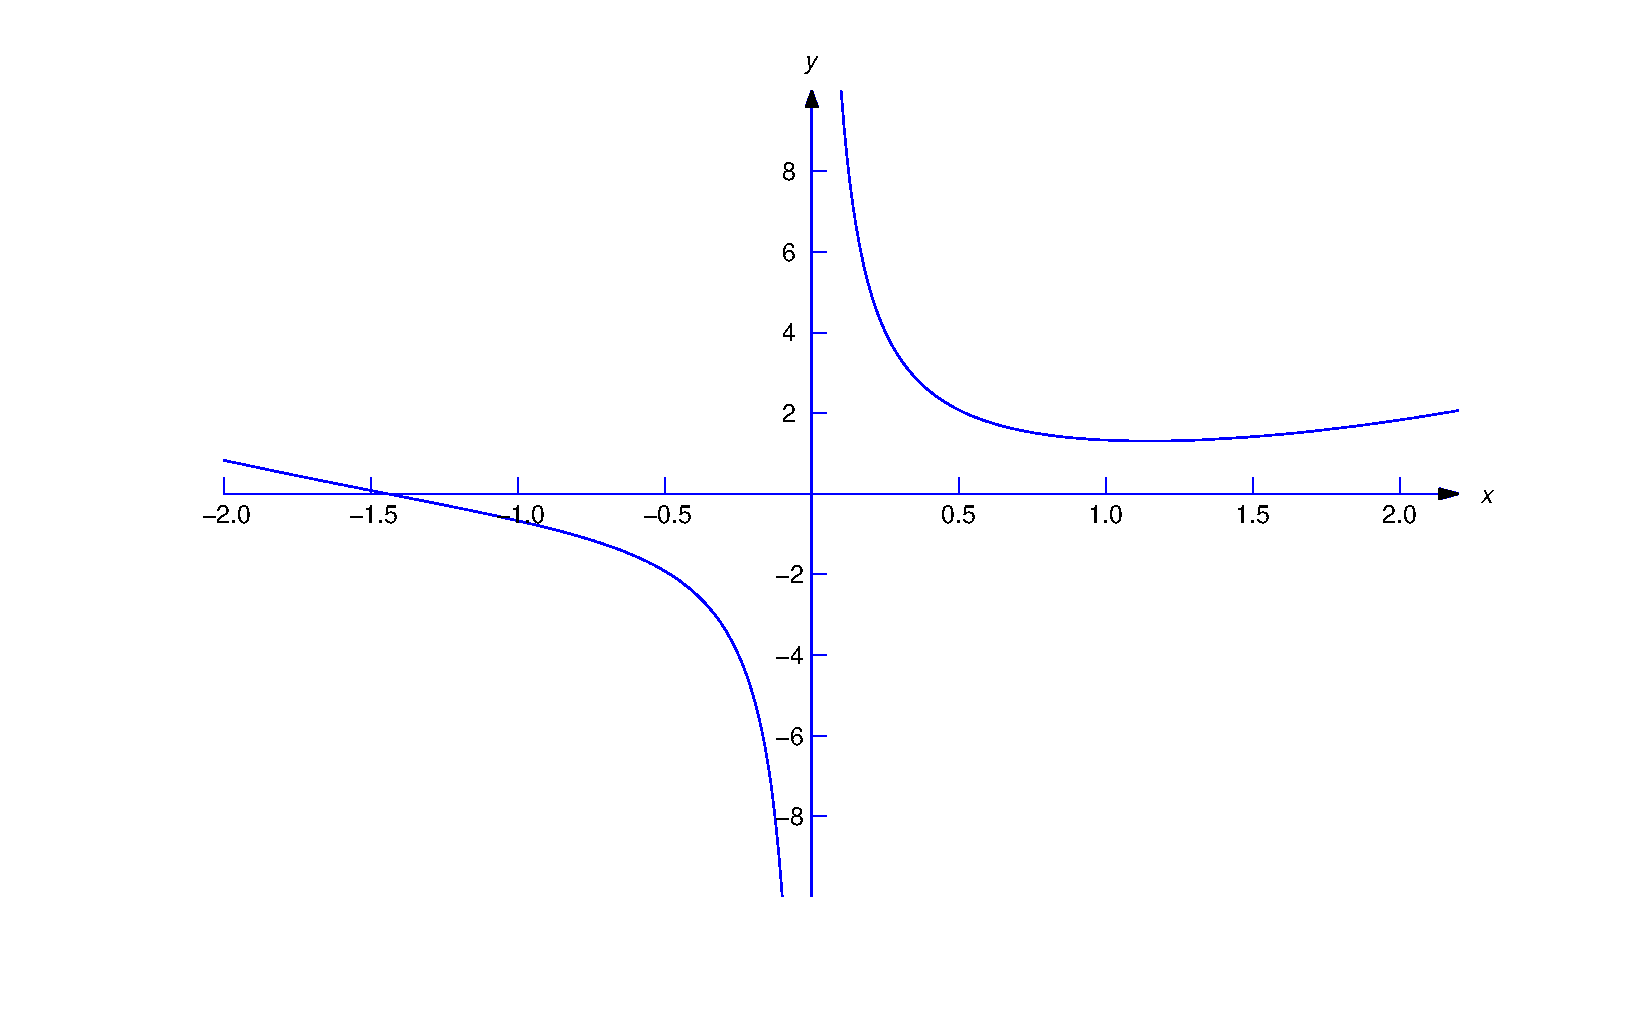
\includegraphics[bb=-78 148 689 643,width=5.67in,height=3.66in,keepaspectratio]{fig010201}
\color{blue}
  \caption{$y=\dst{\frac{x^{2}}{3}+\frac{1}{x}}$}
  \label{figure:1.2.1}
\end{figure}

\solution Differentiating \eqref{eq:1.2.7} twice yields
$$
y'=-(c_1+c_2x)e^{-x}+c_2e^{-x}+2
$$
 and
$$
y''=(c_1+c_2x)e^{-x}-2c_2e^{-x},
$$
so
\begin{eqnarray*}
y''+2y'+y&=&(c_1+c_2x)e^{-x}-2c_2e^{-x}\\
&&+2\left[-(c_1+c_2x)e^{-x}+c_2e^{-x}+2\right]\\
&&+(c_1+c_2x)e^{-x}+2x-4\\
&=&(1-2+1)(c_1+c_2x)e^{-x}+(-2+2)c_2e^{-x}\\ &&+4+2x-4=2x
\end{eqnarray*}
for all values of $x$.
Therefore $y$ is a solution of \eqref{eq:1.2.8} on $(-\infty,\infty)$.

\begin{example}\label{example:1.2.4} \rm
Find all solutions of
\begin{equation} \label{eq:1.2.9}
y^{(n)}=e^{2x}.
\end{equation}
\end{example}

\solution Integrating \eqref{eq:1.2.9} yields
$$
y^{(n-1)}={e^{2x}\over2}+k_1,
$$
 where $k_1$ is a constant. If $n\ge2$,
integrating again yields
$$
y^{(n-2)}={e^{2x}\over4}+k_1x+k_2.
$$
If $n\ge3$, repeatedly integrating yields
\begin{equation} \label{eq:1.2.10}
y={e^{2x}\over2^n}+k_1{x^{n-1}\over (n-1)!}+k_2{x^{n-2}\over
(n-2)!}+\cdots+k_n,
\end{equation}
 where $k_1$, $k_2$, \dots, $k_n$ are constants.
This shows that every solution of \eqref{eq:1.2.9} has the form
\eqref{eq:1.2.10}
for some choice of the constants $k_1$, $k_2$, \dots, $k_n$.
On the other hand, differentiating \eqref{eq:1.2.10}  $n$ times shows
that if
$k_1$, $k_2$, \dots, $k_n$ are arbitrary constants, then the function $y$
in
\eqref{eq:1.2.10} satisfies \eqref{eq:1.2.9}.

Since the constants $k_1$, $k_2$, \dots, $k_n$  in \eqref{eq:1.2.10}
are arbitrary, so are the constants
$${k_1\over (n-1)!},\, {k_2\over(n-2)!},\, \cdots, \, k_n.$$
 Therefore Example~\ref{example:1.2.4} actually shows that all
solutions of \eqref{eq:1.2.9}  can be written as
$$
y={e^{2x}\over2^n}+c_1+c_2x+\cdots+c_nx^{n-1},
$$
 where we  renamed the arbitrary constants in
\eqref{eq:1.2.10} to obtain a simpler formula. As a
general rule, arbitrary constants appearing in solutions  of differential
equations should be simplified if possible. You'll see examples
of this throughout the text.

\boxit{Initial Value Problems}

\noindent
In Example~\ref{example:1.2.4} we saw that the differential equation
$y^{(n)}=e^{2x}$ has an infinite family of solutions that depend upon
the $n$ arbitrary constants $c_1$, $c_2$, \dots, $c_n$. In the absence of
additional conditions, there's no reason to prefer one solution of a
differential equation over another. However, we'll often be
interested in finding a solution of a differential equation that
satisfies one or more specific conditions. The next example
illustrates this.

\begin{example}\label{example:1.2.5} \rm
 Find a solution of
$$
y'=x^3
$$
 such that $y(1)=2$.
\end{example}

\solution  At the beginning of this section we saw
that the  solutions of $y'=x^3$ are
$$
y={x^4\over4}+c.
$$
 To determine a value of $c$ such that $y(1)=2$,
we set $x=1$ and $y=2$ here to obtain
$$
2=y(1)={1\over4}+c,\mbox{\quad so \quad}c={7\over4}.
$$
 Therefore the required solution is
$$
y={x^4+7\over4}.
$$

Figure~\ref{figure:1.2.2} shows
the graph  of this solution.
Note that imposing the  condition $y(1)=2$ is equivalent to requiring
 the graph of $y$ to pass through the point $(1,2)$.

 We can rewrite the problem considered in Example~\ref{example:1.2.5}
more briefly as
$$
y'=x^3,\quad y(1)=2.
$$
 We call this an {\color{blue}\it initial value problem\/}.
The requirement $y(1)=2$ is an {\color{blue}\it initial condition}.
 Initial value problems can also be
posed for higher order differential equations.  For example,
\begin{equation} \label{eq:1.2.11}
y'' - 2y'+3y=e^x, \quad y(0)=1, \quad y'(0)=2
\end{equation}
is  an initial value problem for a second order differential
equation where $y$ and $y'$ are required to have specified values at
 $x=0$. In general, an initial value
problem for an $n$-th order differential equation requires $y$ and its
first $n-1$ derivatives to have specified values at some point $x_0$.
These requirements are the {\color{blue}\it initial conditions\/}.

\begin{figure}[H]
  \centering
  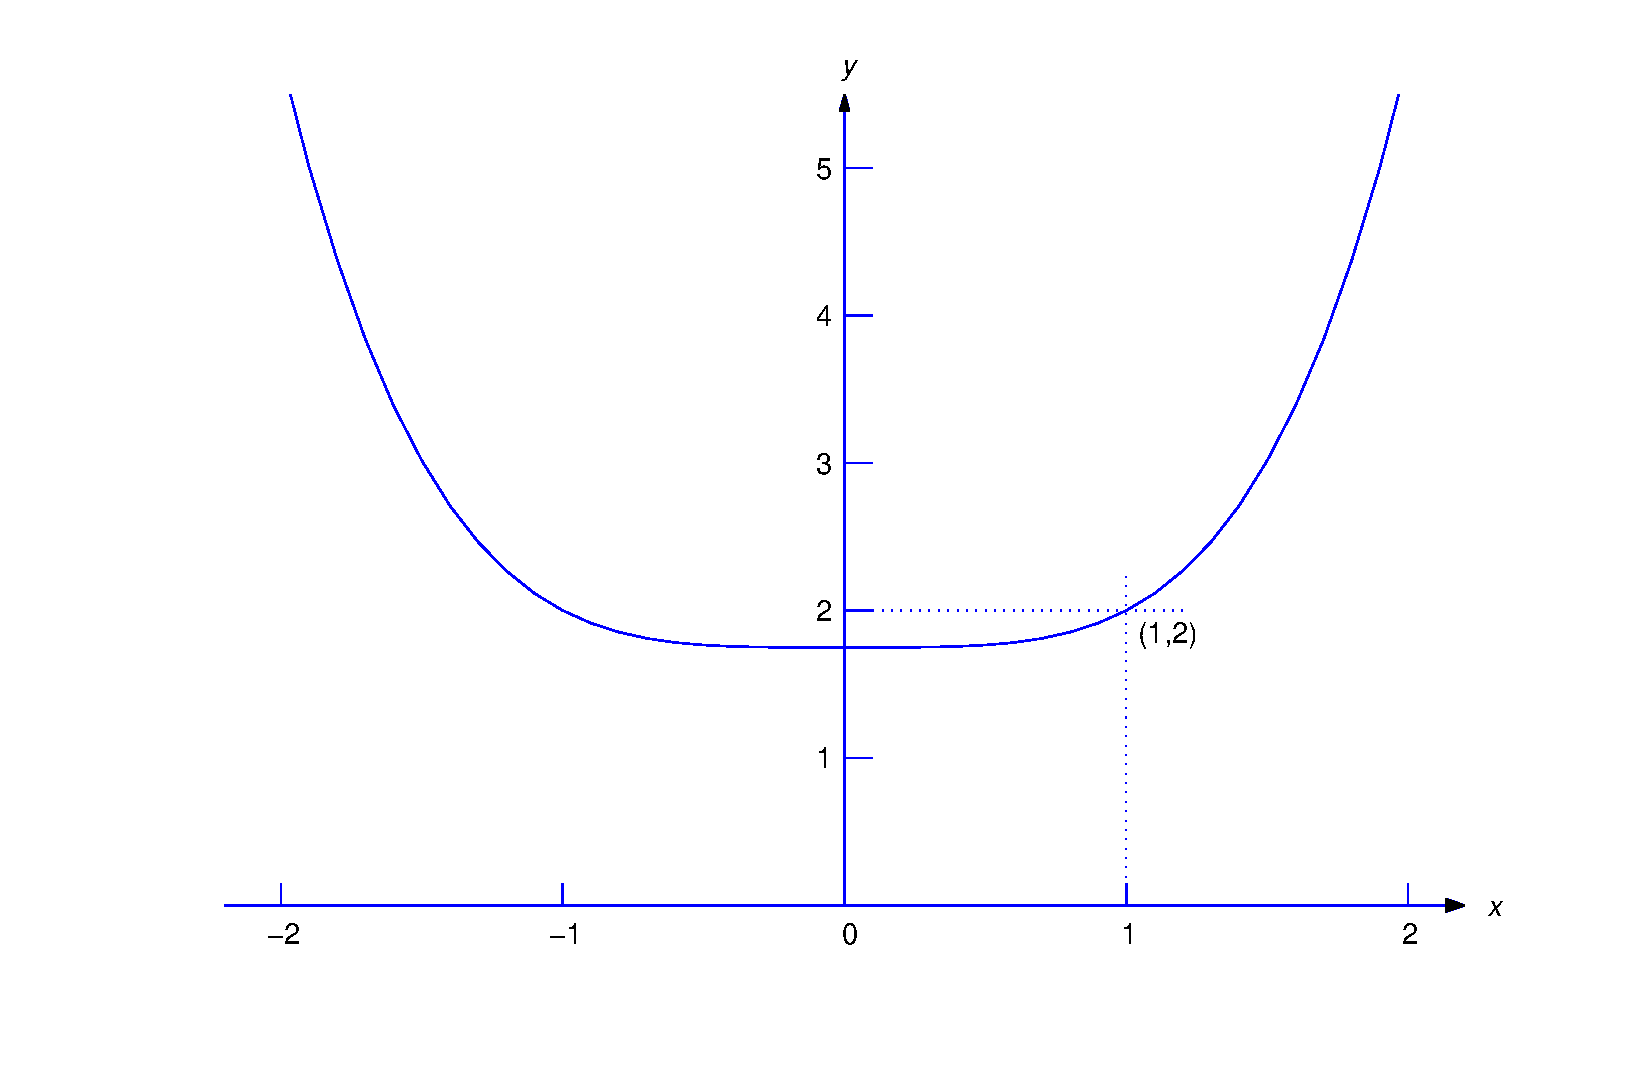
\includegraphics[bb=-78 148 689 643,width=5.67in,height=3.66in,keepaspectratio]{fig010202}
\color{blue}
  \caption{$y=\dst{\frac{x^{2}+7}{4}}$ }
  \label{figure:1.2.2}
\end{figure}

We'll denote an initial value problem for a differential equation by
writing the initial conditions after the equation, as in
\eqref{eq:1.2.11}. For example, we would write an initial value problem
for \eqref{eq:1.2.2} as
\begin{equation} \label{eq:1.2.12}
y^{(n)}=f(x,y,y', \dots,y^{(n-1)}),\, y(x_0)=k_0,\,
y'(x_0)=k_1,\, \dots,\, y^{(n-1)}=k_{n-1}.
\end{equation}
Consistent with our earlier definition of a solution of the
differential equation in \eqref{eq:1.2.12}, we say that $y$ is a solution
of the initial value problem \eqref{eq:1.2.12}  if $y$ is $n$ times
differentiable and
$$
y^{(n)}(x)=f(x,y(x),y'(x), \dots,y^{(n-1)}(x))
$$
for all $x$ in some open interval $(a,b)$  that contains $x_0$,
and  $y$ satisfies the initial conditions in \eqref{eq:1.2.12}. The
largest open interval that contains $x_0$ on which $y$ is defined and
satisfies the differential equation is  the {\color{blue}\it interval of
validity} of $y$.

\begin{example}\label{example:1.2.6} \rm
In Example~\ref{example:1.2.5} we saw that
\begin{equation} \label{eq:1.2.13}
y={x^4+7\over4}
\end{equation}
is a solution of the initial value problem
$$
y'=x^3,\quad y(1)=2.
$$
Since the function in \eqref{eq:1.2.13} is defined for all $x$, the
interval of validity of this solution is $(-\infty,\infty)$.
\end{example}

\begin{example}\label{example:1.2.7} \rm
In Example~\ref{example:1.2.2} we verified that
\begin{equation} \label{eq:1.2.14}
y={x^2\over3}+{1\over x}
\end{equation}
is a solution of
$$
xy'+y=x^2
$$
on $(0,\infty)$ and on $(-\infty,0)$. By evaluating \eqref{eq:1.2.14} at
$x=\pm1$, you can see that \eqref{eq:1.2.14} is a solution of the initial
value problems
\begin{equation} \label{eq:1.2.15}
xy'+y=x^2,\quad y(1)={4\over3}
\end{equation}
and
\begin{equation} \label{eq:1.2.16}
xy'+y=x^2,\quad y(-1)=-{2\over3}.
\end{equation}
The interval of validity of \eqref{eq:1.2.14} as a solution of
\eqref{eq:1.2.15} is $(0,\infty)$, since this is the largest interval
that contains $x_0=1$ on which \eqref{eq:1.2.14} is defined. Similarly, the
interval of validity of \eqref{eq:1.2.14} as a solution of \eqref{eq:1.2.16}
is $(-\infty,0)$, since this is the largest interval that contains
$x_0=-1$ on which \eqref{eq:1.2.14} is defined.
\end{example}

\boxit{Free Fall Under Constant Gravity}

\noindent
The term {\color{blue}\it initial value problem}  originated in problems
of motion where the independent variable is $t$
(representing elapsed time), and the initial conditions
are the position and velocity of an object at the initial
(starting) time of an experiment.

\begin{example}\label{example:1.2.8} \rm
An object falls under the influence of gravity near Earth's
surface, where it can be assumed that the magnitude of the
acceleration due to gravity is a constant $g$.
\begin{alist}
\item % (a)
 Construct a mathematical model for the motion of the object in the
form of an initial value problem for a second order differential
equation, assuming that the altitude and velocity of the object at
time $t=0$ are known. Assume that gravity is the only force acting on
the object.
\item % (b)
 Solve the initial value problem derived in \part{a} to obtain the
altitude as a function of time.
\end{alist}
\end{example}

\solutionpart{a} Let $y(t)$ be the altitude of the object at time $t$.
 Since the acceleration of the object has
constant magnitude $g$ and is in the downward (negative) direction,
$y$ satisfies the second order equation
$$
y''=-g,
$$
where the prime now indicates differentiation with respect to $t$.
If $y_0$ and $v_0$ denote the altitude and velocity when
$t=0$, then $y$ is a solution of the initial value problem
\begin{equation} \label{eq:1.2.17}
y''=-g,\quad  y(0)=y_0,\quad y'(0)=v_0.
\end{equation}

\solutionpart{b}
Integrating \eqref{eq:1.2.17} twice yields
\begin{eqnarray*}
y'&=&-gt+c_1, \\
y&=&-{gt^2\over2}+c_1t+c_2.
\end{eqnarray*}
Imposing the initial conditions $y(0)=y_0$ and $y'(0)=v_0$ in these
two equations shows that $c_1=v_0$ and $c_2=y_0$. Therefore the
solution of the initial value problem \eqref{eq:1.2.17} is
$$
y=- {gt^2\over2}+v_0t+y_0.
$$

\exercises
\begin{exerciselist}
\item\label{exer:1.2.1}
Find the order of the   equation.

\begin{tabular}[t]{@{}p{168pt}@{}p{168pt}}
{\bf (a)}\   $\dst{d^2y\over dx^2}+2
{dy\over dx}\   {d^3y\over dx^3}+x=0$
& {\bf (b)}\   $y''-3y'+2y=x^7$\\[9pt]
{\bf (c)}\   $y'-y^7=0$
& {\bf (d)}\   $y''y-(y')^2=2$
\end{tabular}

\item\label{exer:1.2.2}
Verify that the  function is a solution of the
differential equation on some interval, for any choice of
the arbitrary constants appearing in the function.

\begin{alist}
\item % (a)
 $y=ce^{2x};     \quad y'=2y$
\item % (b)
 $y=\dst{x^2\over3}
+{c\over x};   \quad xy'+y=x^2$

\item %(c)
$y=\dst{1\over2}+ce^{-x^2};    \quad y'+2xy=x$

\item %(d)
$y=(1+ce^{-x^2/2});   (1-ce^{-x^2/2})^{-1}   \quad
2y'+x(y^2-1)=0$

\item %(e)
$y=\dst{\tan\left( {x^3\over3}+c\right)};     \quad
y'=x^2(1+y^2)$

\item %(f)
$y=(c_1+c_2x)e^x+\sin x+x^2;    \quad
y''-2y'+y=-2 \cos x+x^2-4x+2$

\item %(g)
$y=c_1e^x+c_2x+\dst{2\over x};     \quad
(1-x)y''+xy'- y=4(1-x-x^2)x^{-3}$

\item %(h)
$y=x^{-1/2}(c_1\sin x+c_2 \cos x)+4x+8$;     \newline
$x^2y''+xy'+\dst{\left(x^2-{1\over4}\right)}y=4x^3+8x^2+3x-2$
\end{alist}

\item\label{exer:1.2.3}
Find all solutions of the  equation.

\begin{tabular}[t]{@{}p{168pt}@{}p{168pt}}
{\bf (a)}\quad  $y'=-x$
& {\bf (b)}\quad  $y'=-x \sin x$\\
{\bf (c)}\quad  $y'=x \ln x$
& {\bf (d)}\quad  $y''=x \cos x$\\
{\bf (e)}\quad  $y''=2xe^x$
& {\bf (f)}\quad  $y''=2x+\sin x+e^x$\\
{\bf (g)}\quad  $y'''=-\cos x$
& {\bf (h)}\quad  $y'''=-x^2+e^x$\\
{\bf (i)}\quad  $y'''=7e^{4x}$&
\end{tabular}

\item\label{exer:1.2.4}
Solve the  initial value problem.

\begin{alist}
\item % (a)
 $y'=-xe^x, \quad y(0)=1$
\item % (b)
 $\dst{y'=x \sin x^2, \quad y\left({\sqrt{\pi\over2}}\right)=1}$

\item %(c)
$y'=\tan x, \quad y(\pi/4)=3$

\item %(d)
$y''=x^4, \quad y(2)=-1, \quad y'(2)=-1$

\item %(e)
$y''=xe^{2x}, \quad y(0)=7, \quad y'(0)=1$

\item %(f)
$y''=- x \sin x, \quad y(0)=1, \quad y'(0)=-3$

\item %(g)
$y'''=x^2e^x, \quad y(0)=1, \quad y'(0)=-2, \quad
y''(0)=3$

\item %(h)
$y'''=2+\sin 2x, \quad y(0)=1, \quad y'(0)=-6, \quad
y''(0)=3$

\item %(i)
$y'''=2x+1, \quad y(2)=1, \quad
y'(2)=-4, \quad y''(2)=7$
\end{alist}

\item\label{exer:1.2.5}
Verify that the  function is a solution of
the initial value problem.

\begin{alist}
\item %(a)
$y=x\cos x;     \quad y'=\cos x-y\tan x, \quad
y(\pi/4)=\dst{\pi\over4\sqrt{2}}$

\item %(b)
$\dst{y={1+2\ln x\over x^2}+{1\over2};     \quad
y'={x^2-2x^2y+2\over x^3},   \quad y(1)={3\over2}}$

\item %(c)
$y=\dst{\tan\left({x^2\over2}\right)};
\quad y'=x(1+y^2),   \quad y(0)=0$

\item %(d)
$\dst{y={2\over x-2};     \quad y'={-y(y+1)\over x}}, \quad
y(1)=-2$
\end{alist}

\item\label{exer:1.2.6}
Verify that the  function is a solution of
the initial value problem.

\begin{alist}
\item %(a)
$y=x^2(1+\ln x);     \quad y''=\dst{3xy'-4y\over x^2}, \quad
y(e)=2e^2, \quad y'(e)=5e$

\item %(b)
$y=\dst{x^2\over3}+x-1;     \quad y''=\dst{x^2-xy'+y+1\over
x^2}, \quad y(1)=\dst{1\over3}, \quad y'(1)=\dst{5\over3}$

\item %(c)
$y=(1+x^2)^{-1/2};     \quad
y''=\dst{(x^2-1)y-x(x^2+1)y'\over (x^2+1)^2}, \quad y(0)=1,$

$y'(0)=0$

\item %(d)
$y=\dst{x^2\over 1-x};    \quad y''=\dst{2(x+y)(xy'-y)\over x^3},
\quad y(1/2)=1/2, \quad y'(1/2)=3$
\end{alist}

\item\label{exer:1.2.7}
Suppose an object is launched from a point 320 feet
above the earth with an initial velocity of 128 ft/sec
upward, and  the only force acting on it thereafter is
gravity. Take $g=32$ ft/sec$^2$.

\begin{alist}
\item %(a)
Find the highest altitude attained by the object.

\item %(b)
Determine how long it takes for the object to fall to the
ground.
\end{alist}

\item\label{exer:1.2.8}
\setcounter{equation}{0}
Let $a$ be a nonzero real number.
\begin{alist}
\item % (a)
Verify that if $c$ is an arbitrary constant then
$$
y=(x-c)^a
\eqno{\rm (A)}
$$
is a solution of
$$
y'=ay^{(a-1)/a}
\eqno{\rm (B)}
$$
on $(c,\infty)$.
\item % (b)
Suppose $a<0$ or $a>1$. Can you think of a solution of
(B) that isn't of the form (A)?
\end{alist}

\item\label{exer:1.2.9}
Verify that
$$
y=
\left\{ \begin{array}{cl}
e^x-1,& x \ge 0, \\[6pt]
1-e^{-x},& x < 0, \end{array}\right.
$$
is a solution of
$$
y'=|y|+1
$$
on $(-\infty,\infty)$. \hint{Use the definition of derivative
at $x=0$.}

\item\label{exer:1.2.10}
\begin{alist}
\item %(a)
Verify that if $c$ is any real number then
$$
y=c^2+cx+2c+1
\eqno{\rm (A)}
$$
satisfies
$$
 y'={-(x+2)+\sqrt{x^2+4x+4y}\over2}
\eqno{\rm (B)}
$$
on some open interval. Identify the open interval.

\item %(b)
Verify that
$$
y_1={-x(x+4)\over4}
$$
also satisfies  (B) on some open interval, and
identify the open interval. (Note that $y_1$ can't be obtained
by selecting a value of $c$ in (A).)
\end{alist}

\end{exerciselist}

\newsection{3}{Introduction} {Direction Fields for First Order Equations}
\currentpdfbookmark{Section 1.3 Direction Fields for First Order Equations}{section:1.3}
\vskip14pt
\renewcommand{\thissection}{\sectiontitle{\,
DIRECTION FIELDS FOR FIRST ORDER EQUATIONS}}
\thissection

\noindent
It's impossible to find explicit formulas for solutions of some
differential equations. Even if there are such  formulas, they may be
so complicated that they're useless. In this case we may resort to
graphical or numerical methods to get some idea of how the solutions
of the given equation behave.

 In Section~2.3 we'll take up
the question of existence of solutions of a first order equation
\begin{equation} \label{eq:1.3.1}
y'=f(x,y).
\end{equation}
In this section we'll simply assume that \eqref{eq:1.3.1} has
solutions and discuss a graphical method for approximating them.
In Chapter~3 we discuss numerical methods for obtaining
approximate solutions of \eqref{eq:1.3.1}.

Recall that a solution of \eqref{eq:1.3.1} is a function $y=y(x)$ such
that
$$
y'(x)=f(x,y(x))
$$
for all values of $x$ in some interval, and an integral curve is
either the graph of a solution or is
made up of  segments that are graphs of solutions.
 Therefore, not being able to
solve \eqref{eq:1.3.1} is equivalent to not knowing the equations of
integral curves of \eqref{eq:1.3.1}. However, it's easy to calculate the
slopes of these curves. To be specific, the slope of an integral curve
of \eqref{eq:1.3.1} through a given point $(x_0,y_0)$ is given by the
number $f(x_0,y_0)$. This is the basis of {\color{blue}\it the method of direction
fields\/}.

If $f$ is defined on a set $R$, we can construct a {\color{blue}\it direction
field \/} for \eqref{eq:1.3.1}  in $R$ by drawing a
short
line segment through each point $(x,y)$ in $R$ with slope $f(x,y)$. Of
course, as a practical matter, we can't actually draw line segments
through {\color{blue}\it every\/} point in $R$;     rather, we must select
a finite
set of points in $R$. For example, suppose   $f$ is defined on the
closed rectangular region
$$
R:\{a\le x\le b, c\le y\le d\}.
$$
Let
$$
a= x_0< x_1< \cdots< x_m=b
$$
be  equally spaced points in $[a,b]$ and
$$
c=y_0<y_1<\cdots<y_n=d
$$
be  equally spaced points in $[c,d]$.
 We say that the points
$$
 (x_i,y_j),\quad 0\le i\le m,\quad 0\le j\le n,
$$
form a {\color{blue}\it rectangular grid\/} (Figure~\ref{figure:1.3.1}). Through each
point in the grid we draw a short line segment with slope
$f(x_i,y_j)$. The result is an approximation to a direction field  for
\eqref{eq:1.3.1} in $R$. If the grid points are sufficiently numerous and
close together, we can draw approximate integral curves of \eqref{eq:1.3.1}
by drawing curves through points in the grid tangent to the line
segments associated with the points in the grid.

\begin{figure}[H]
  \centering
  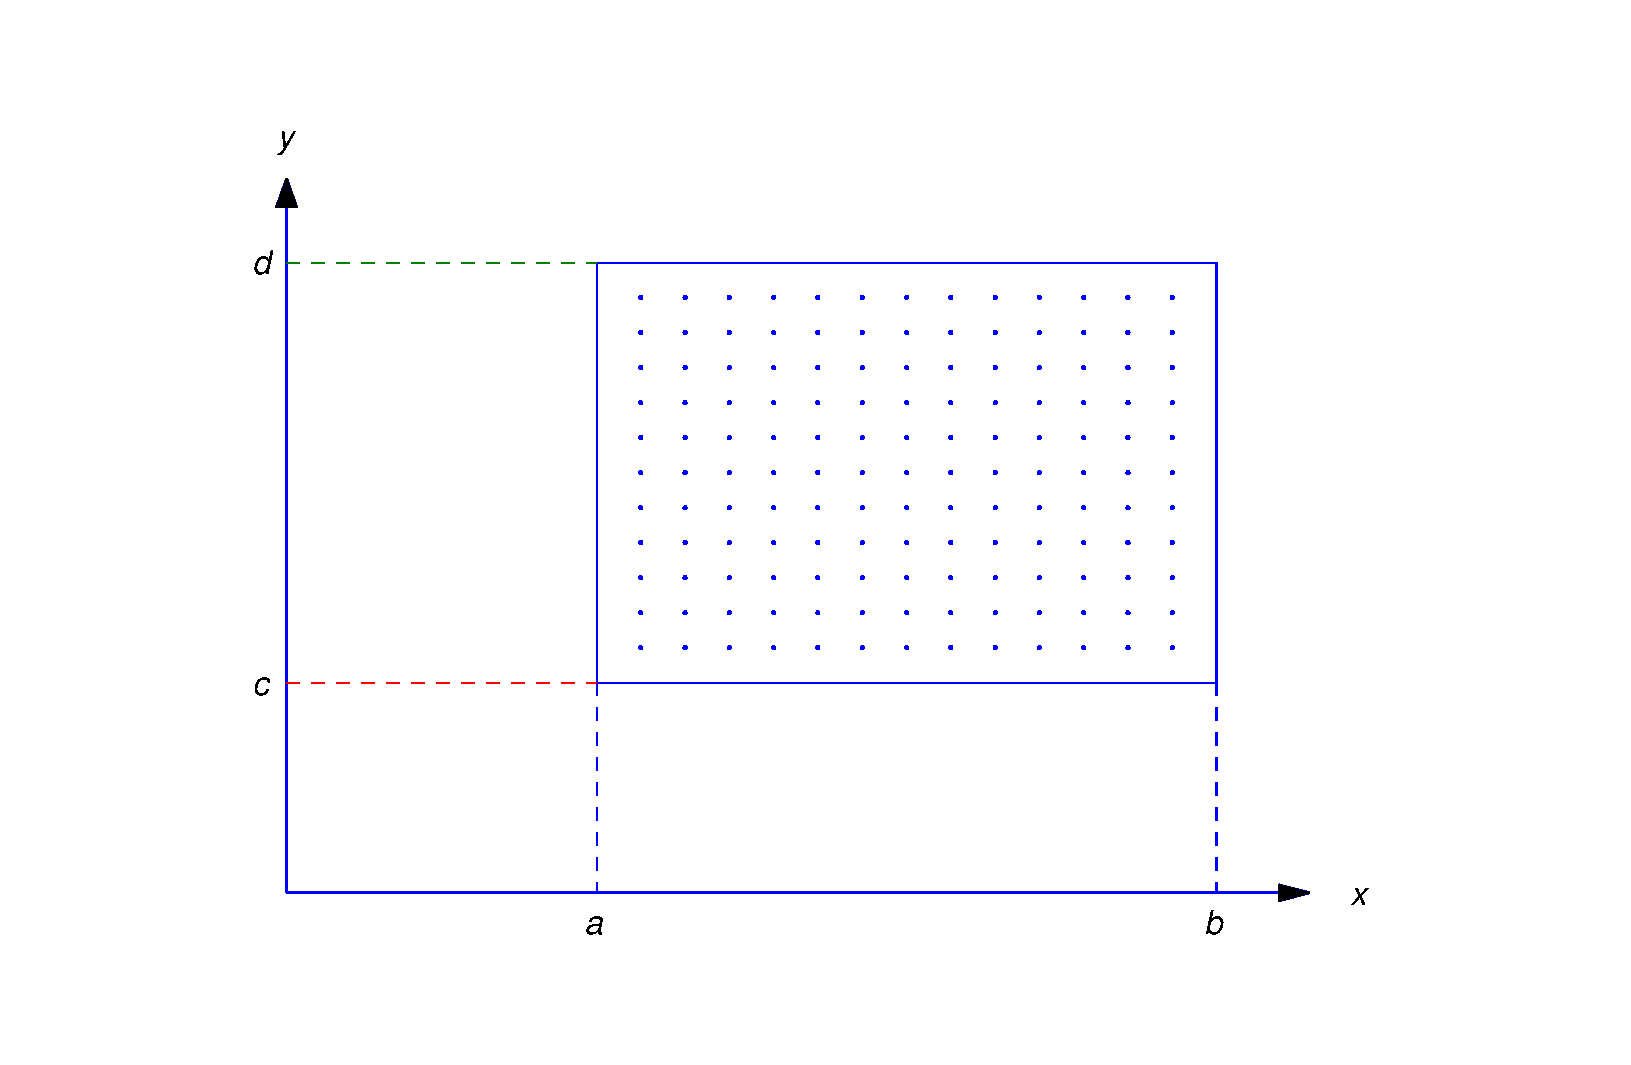
\includegraphics[width = 0.7\textwidth]{fig010301}
\color{blue}
  \caption{\quad  A rectangular grid}
  \label{figure:1.3.1}
\end{figure}

Unfortunately, approximating a direction field and graphing integral
curves in this way is too tedious to be done effectively by hand.
However, there is software  for doing this.
As you'll  see, the combination of  direction fields and
 integral curves gives  useful insights into the behavior of
the solutions of the differential equation even if
we can't obtain exact solutions.

We'll  study numerical methods for solving a single first order
equation \eqref{eq:1.3.1} in Chapter~3. These methods can be
used
to plot solution curves of \eqref{eq:1.3.1} in a rectangular region $R$
{\color{blue}\it if $f$ is continuous on\/} $R$. Figures~\ref{figure:1.3.2},
\ref{figure:1.3.3}, and \ref{figure:1.3.4} show direction fields and solution
curves for the differential equations
$$
 y'=\frac{x^2-y^2}{1+x^2+y^2}, \quad
y'=1+xy^2,\text{\quad and \quad}
 y'=\frac{x-y}{1+x^2},
$$
which are all of the form \eqref{eq:1.3.1} with $f$
 continuous for all $(x,y)$.

\begin{figure}[htbp]
\color{blue}
  \begin{minipage}[b]{0.5\linewidth}
    \centering
   \scalebox{.6}{
  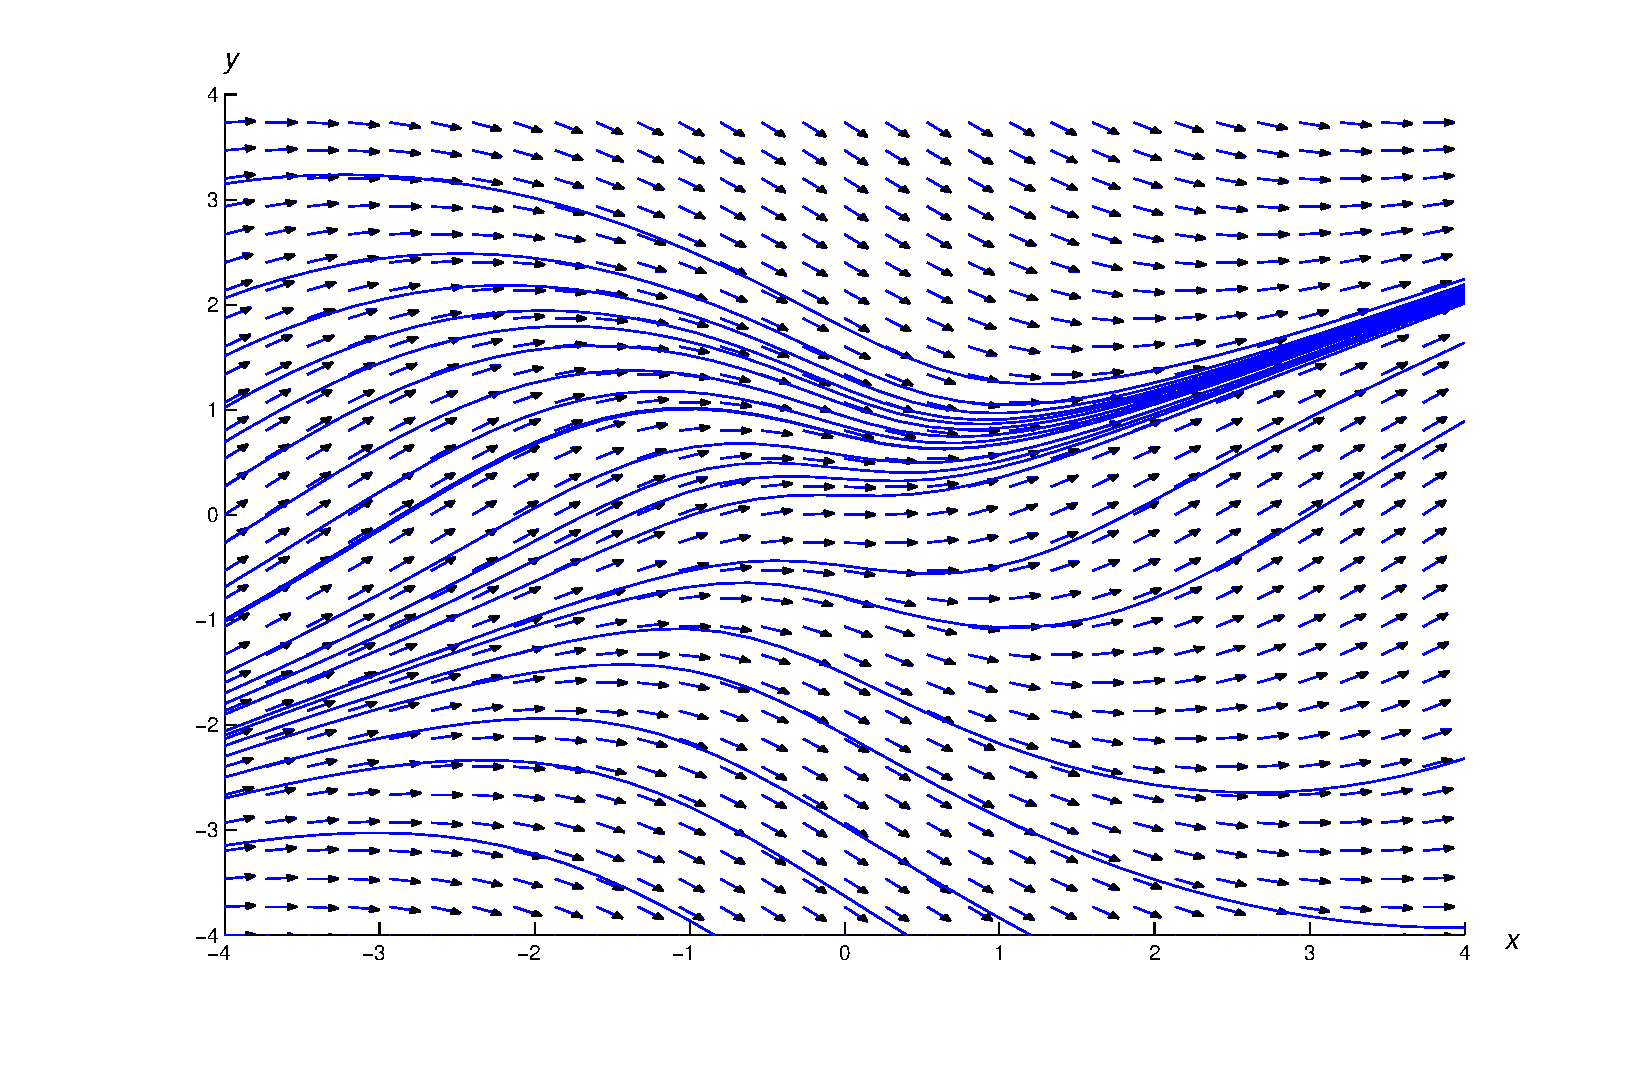
\includegraphics[bb=-78 148 689 643,width=5.67in,height=3.66in,keepaspectratio]{fig010302}}
  \caption{\,A direction field and integral curves for
$y =\dst{\frac{x^{2}-y^{2}}{1+x^{2}+y^{2}}}$}
  \label{figure:1.3.2}
  \end{minipage}
  \hspace{0.6cm}
  \begin{minipage}[b]{0.5\linewidth}
    \centering
   \scalebox{.7}{
  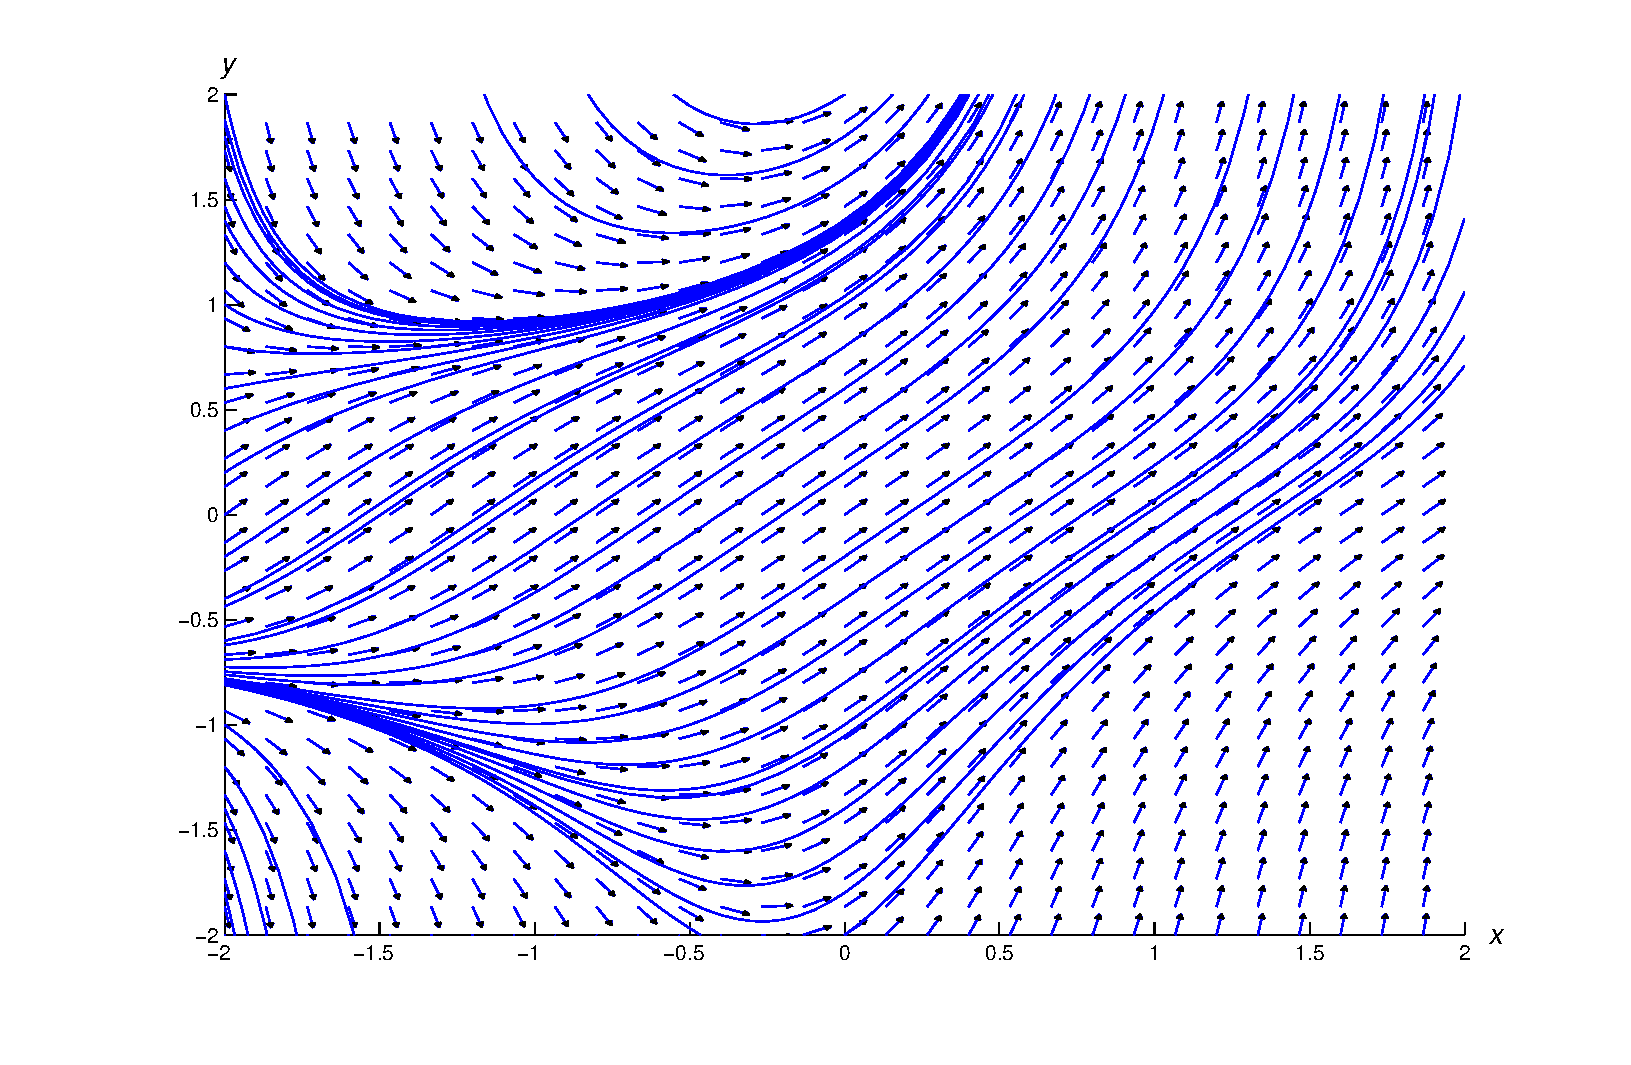
\includegraphics[bb=-78 148 689 643,width=5.67in,height=3.66in,keepaspectratio]{fig010303}}
\caption{A direction field and integral curves
for $y'=1+xy^2$}
  \label{figure:1.3.3}
  \end{minipage}
\end{figure}

\begin{figure}[tbp]
  \centering
  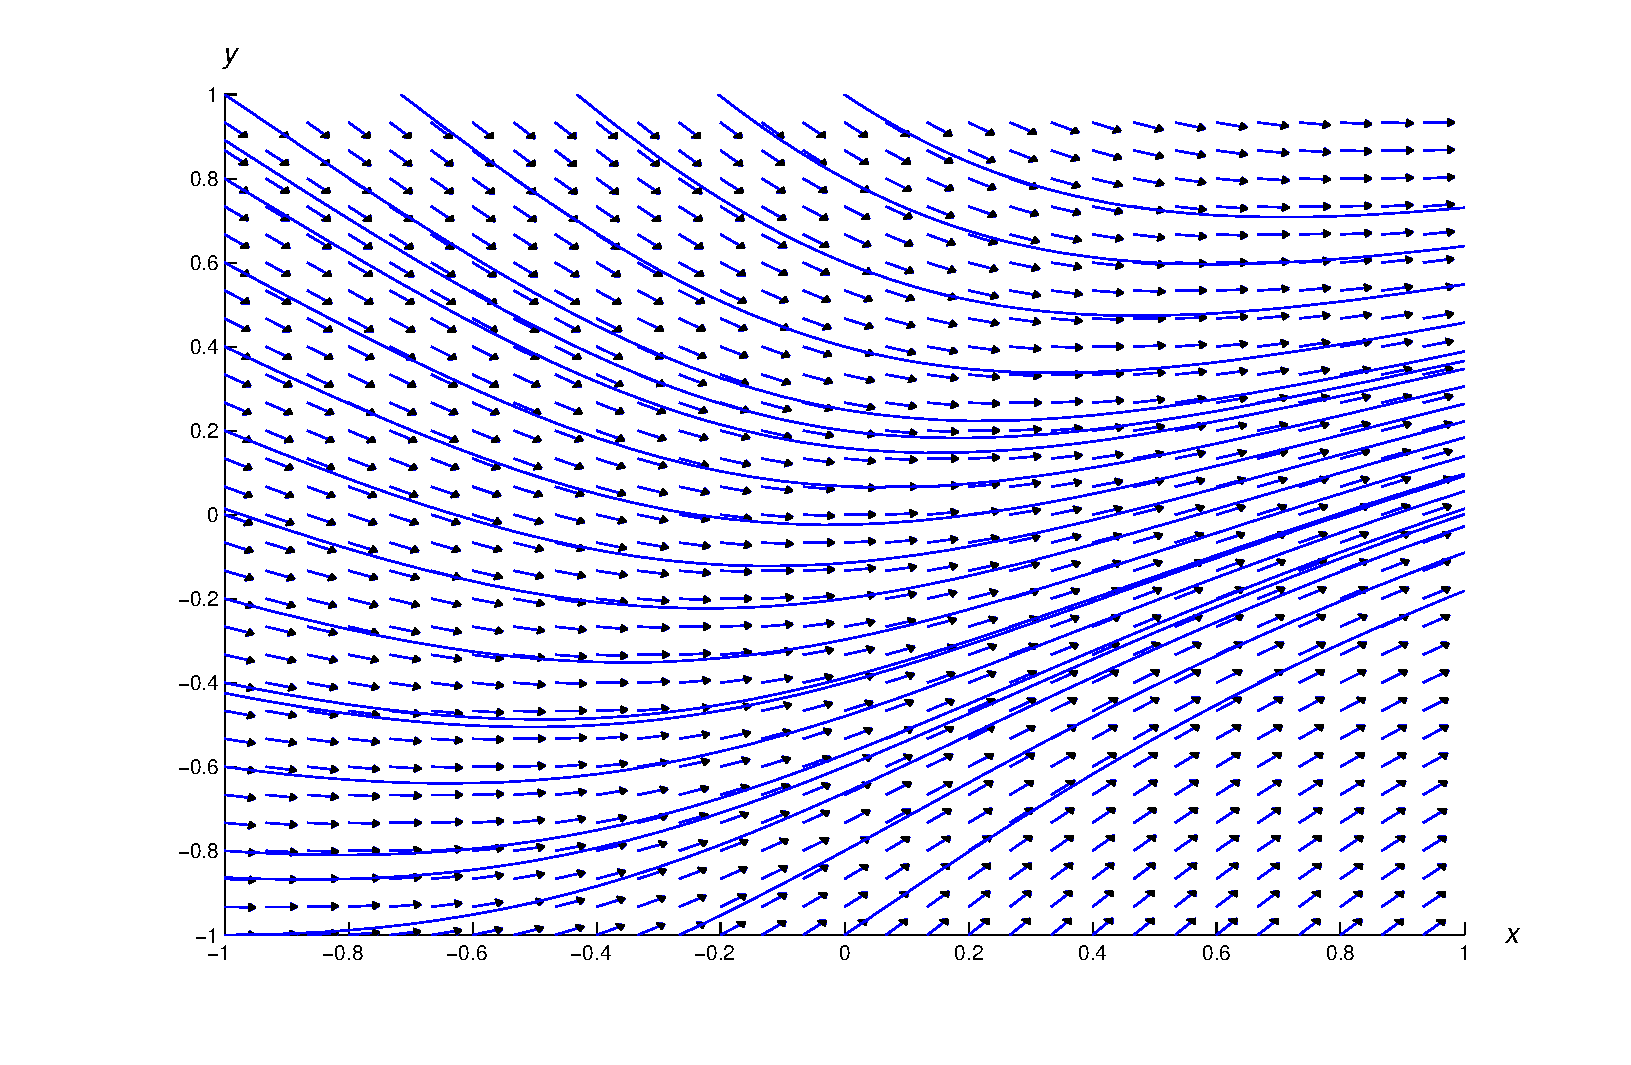
\includegraphics[bb=-78 148 689 643,width=5.67in,height=3.66in,keepaspectratio]{fig010304}
\color{blue}
  \caption{A direction and integral curves for
$y'=\dst{\frac{x-y}{1+x^2}}$}
  \label{figure:1.3.4}
\end{figure}

The methods of Chapter~3 won't work for the equation
\begin{equation} \label{eq:1.3.2}
y'=-x/y
\end{equation}
if $R$ contains part of the $x$-axis, since $f(x,y)=-x/y$ is undefined
when $y=0$. Similarly, they won't work for the equation
\begin{equation} \label{eq:1.3.3}
y'={x^2\over1-x^2-y^2}
\end{equation}
if $R$ contains any part of the unit circle $x^2+y^2=1$, because the
right side of \eqref{eq:1.3.3} is undefined if $x^2+y^2=1$. However,
\eqref{eq:1.3.2} and \eqref{eq:1.3.3} can written as
\begin{equation} \label{eq:1.3.4}
y'={A(x,y)\over B(x,y)}
\end{equation}
where $A$ and $B$ are  continuous on any rectangle $R$. Because of
this,
some differential equation software is based on
numerically solving pairs of equations of the form
\begin{equation} \label{eq:1.3.5}
{dx\over dt}=B(x,y),\quad {dy\over dt}=A(x,y)
\end{equation}
where $x$ and $y$ are regarded as functions of a parameter $t$.
If $x=x(t)$ and $y=y(t)$  satisfy these equations, then
$$
y'={dy\over dx}={dy\over dt}\left/{dx\over dt}\right.={A(x,y)\over
B(x,y)},
$$
so $y=y(x)$ satisfies \eqref{eq:1.3.4}.



Eqns.~\eqref{eq:1.3.2} and \eqref{eq:1.3.3} can be reformulated as in
\eqref{eq:1.3.4} with
$$
{dx\over dt}=-y,\quad {dy\over dt}=x
$$
and
$$
{dx\over dt}=1-x^2-y^2,\quad {dy\over dt}=x^2,
$$
respectively. Even if $f$ is continuous and otherwise ``nice''
throughout $R$, your software  may require you to
reformulate the equation $y'=f(x,y)$ as
$$
{dx\over dt}=1,\quad {dy\over dt}=f(x,y),
$$
which is of the form \eqref{eq:1.3.5} with $A(x,y)=f(x,y)$ and
$B(x,y)=1$.

Figure~\ref{figure:1.3.5} shows a direction field and some integral curves
for \eqref{eq:1.3.2}. As we saw in
Example~\ref{example:1.2.1} and will verify
again in Section~2.2, the integral curves of \eqref{eq:1.3.2}
are circles centered at the origin.



\begin{figure}[H]
  \centering
  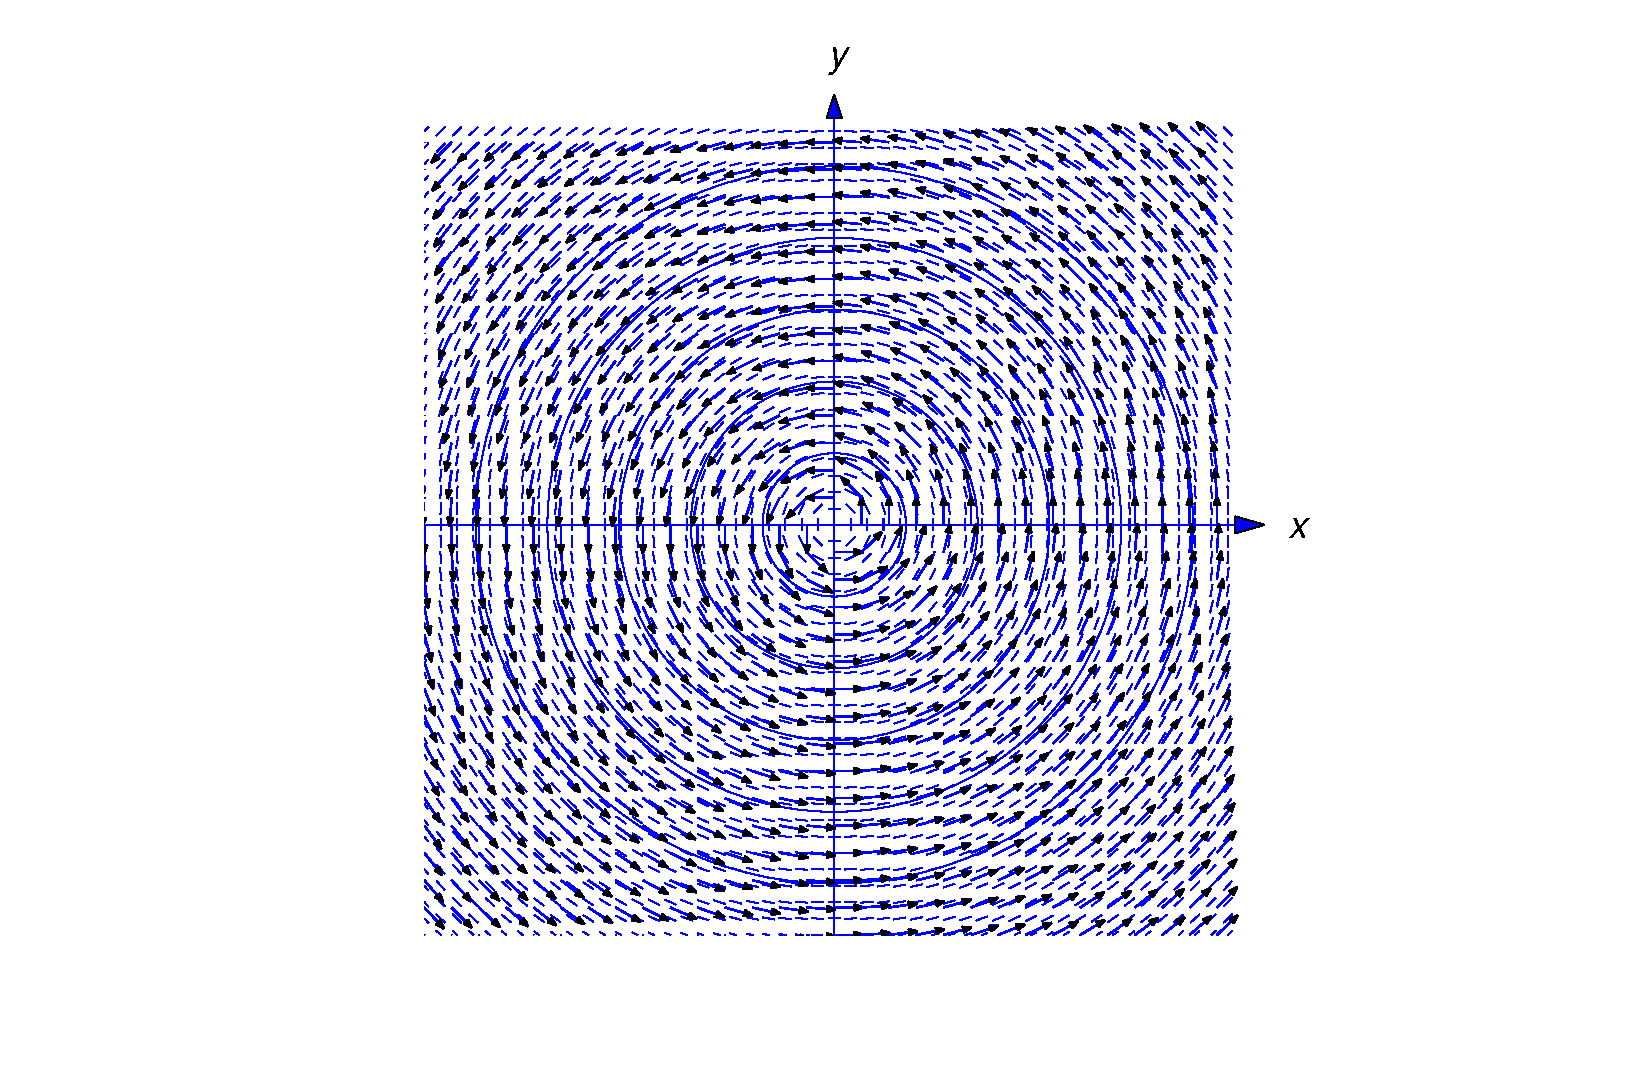
\includegraphics[bb=-78 148 689 643,width=5.67in,height=3.66in,keepaspectratio]{fig010305}
\color{blue}
\caption{A direction field and integral curves for
$y'=-\dst{x\over y}$}
  \label{figure:1.3.5}
\end{figure}

Figure~\ref{figure:1.3.6} shows a direction field and some integral curves
for \eqref{eq:1.3.3}. The integral curves near the top and bottom are
solution curves. However, the integral curves near the middle are more
complicated. For example, Figure~\ref{figure:1.3.7} shows the integral
curve through the origin. The vertices of the dashed rectangle are on
the circle $x^2+y^2=1$ ($a\approx.846$, $b\approx.533$), where all
integral curves of \eqref{eq:1.3.3} have infinite slope. There are
three solution curves of \eqref{eq:1.3.3} on the integral curve in the
figure: the segment above the level $y=b$ is the graph of a solution
on $(-\infty,a)$, the segment below the level $y=-b$ is the graph of a
solution on $(-a,\infty)$, and the segment between these two levels is
the graph of a solution on $(-a,a)$.

\technology
 \medskip
As you study from this book, you'll often be asked to use
computer software and graphics. Exercises with this intent are marked
as \Cex\, (computer or calculator required), \CGex\, (computer and/or
graphics required), or \Lex\ (laboratory work requiring software
and/or graphics).
 Often
you may not completely understand how the software does what it does.
This is similar to the situation most people are in when they drive
automobiles or watch television, and it doesn't decrease the value
of using modern technology as an aid to learning. Just be careful that
you use the technology as a supplement to thought rather than a
substitute for it.


\begin{figure}[htbp]
\color{blue}
  \begin{minipage}[b]{0.5\linewidth}
    \centering
   \scalebox{.7}{
  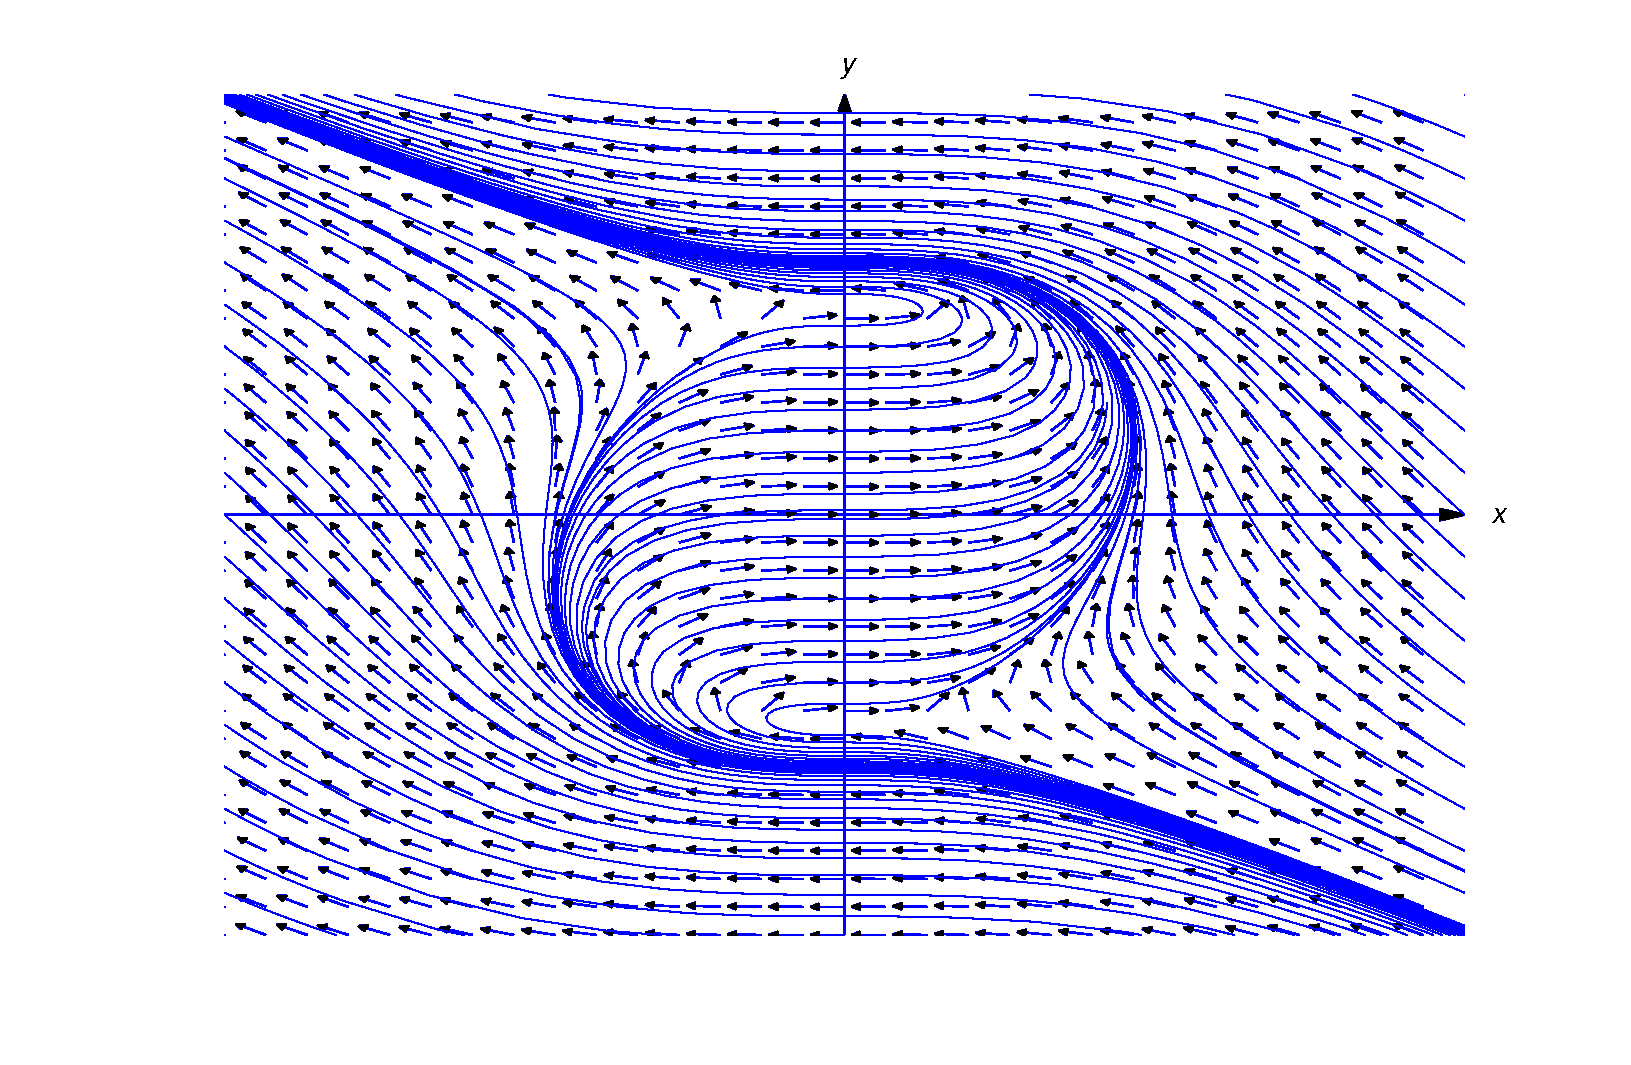
\includegraphics[bb=-78 148 689 643,width=5.67in,height=3.66in,keepaspectratio]{fig010306} }
\caption{A direction field and integral curves for
$y'=\dst{x^2\over1-x^2-y^2}$}
  \label{figure:1.3.6}
  \end{minipage}
  \hspace{0.6cm}
  \begin{minipage}[b]{0.5\linewidth}
    \centering
   \scalebox{.7}{
  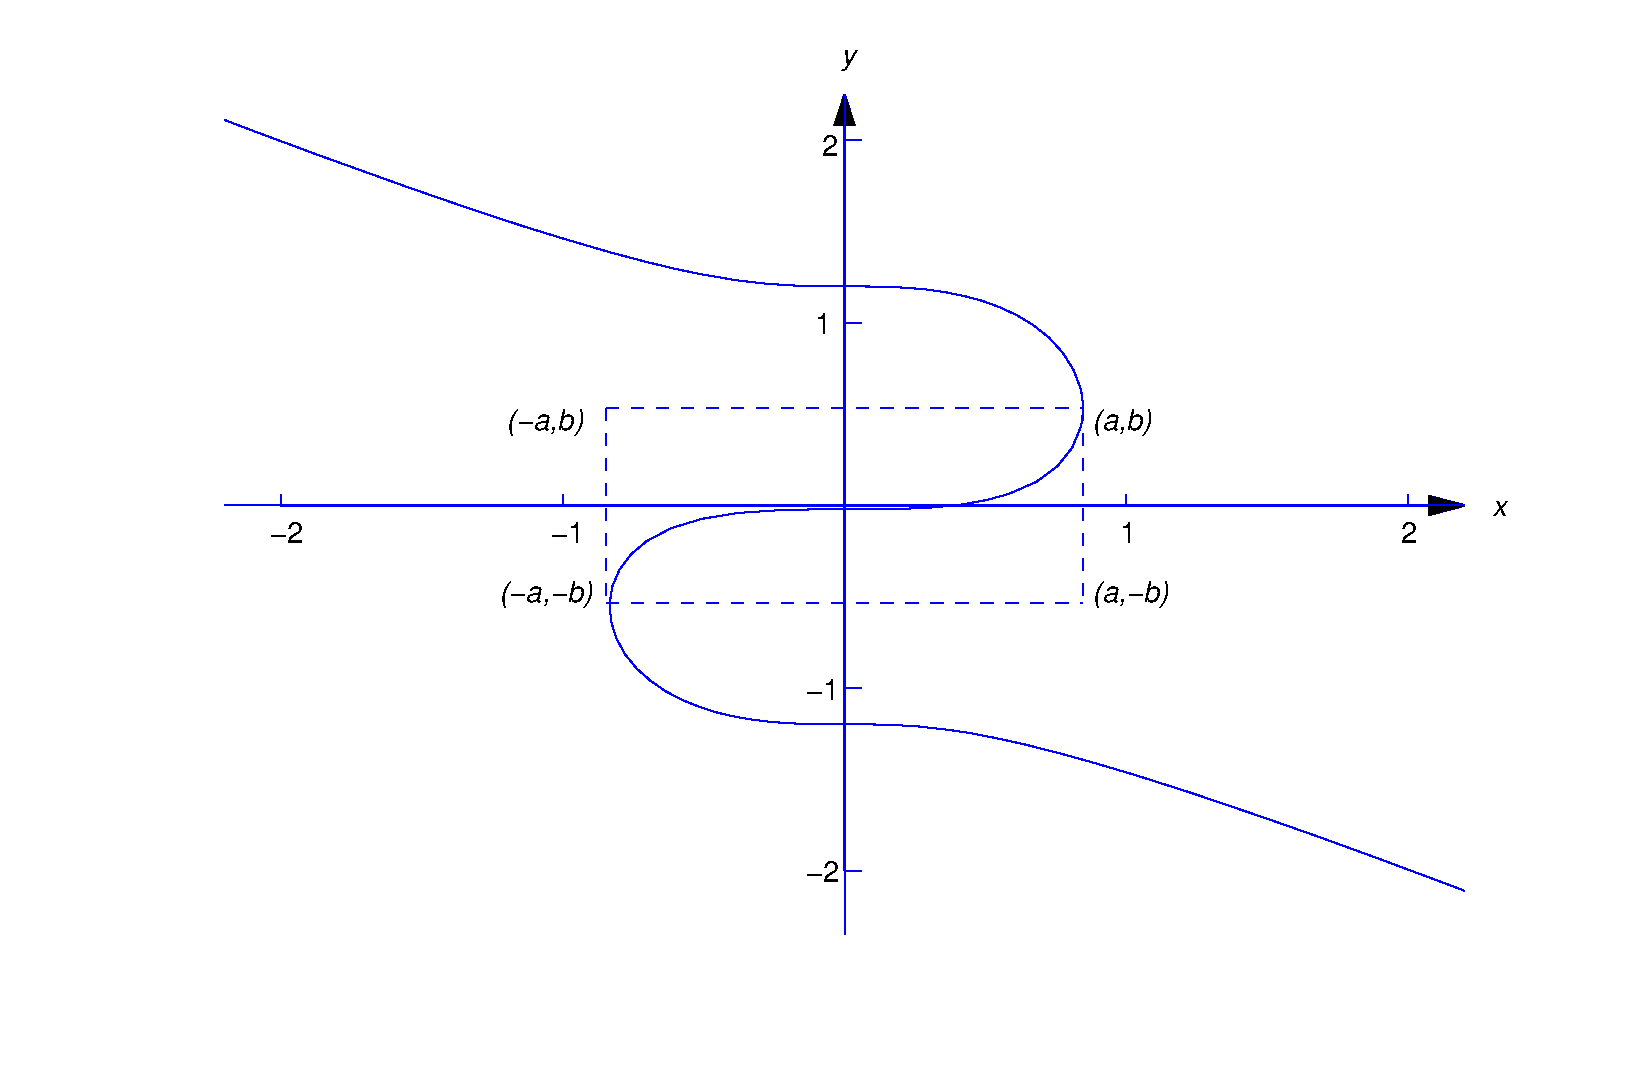
\includegraphics[bb=-78 148 689 643,width=5.67in,height=3.66in,keepaspectratio]{fig010307} }
\caption{}
  \label{figure:1.3.7}
  \end{minipage}
\end{figure}

\enlargethispage{1in}

\exercises
\noindent
\emph{In Exercises~{\color{red}\rm\bf 1--11} a  direction
field is drawn for the given equation. Sketch some integral curves.}



\begin{figure}[H]
  \color{blue}
  \centering
  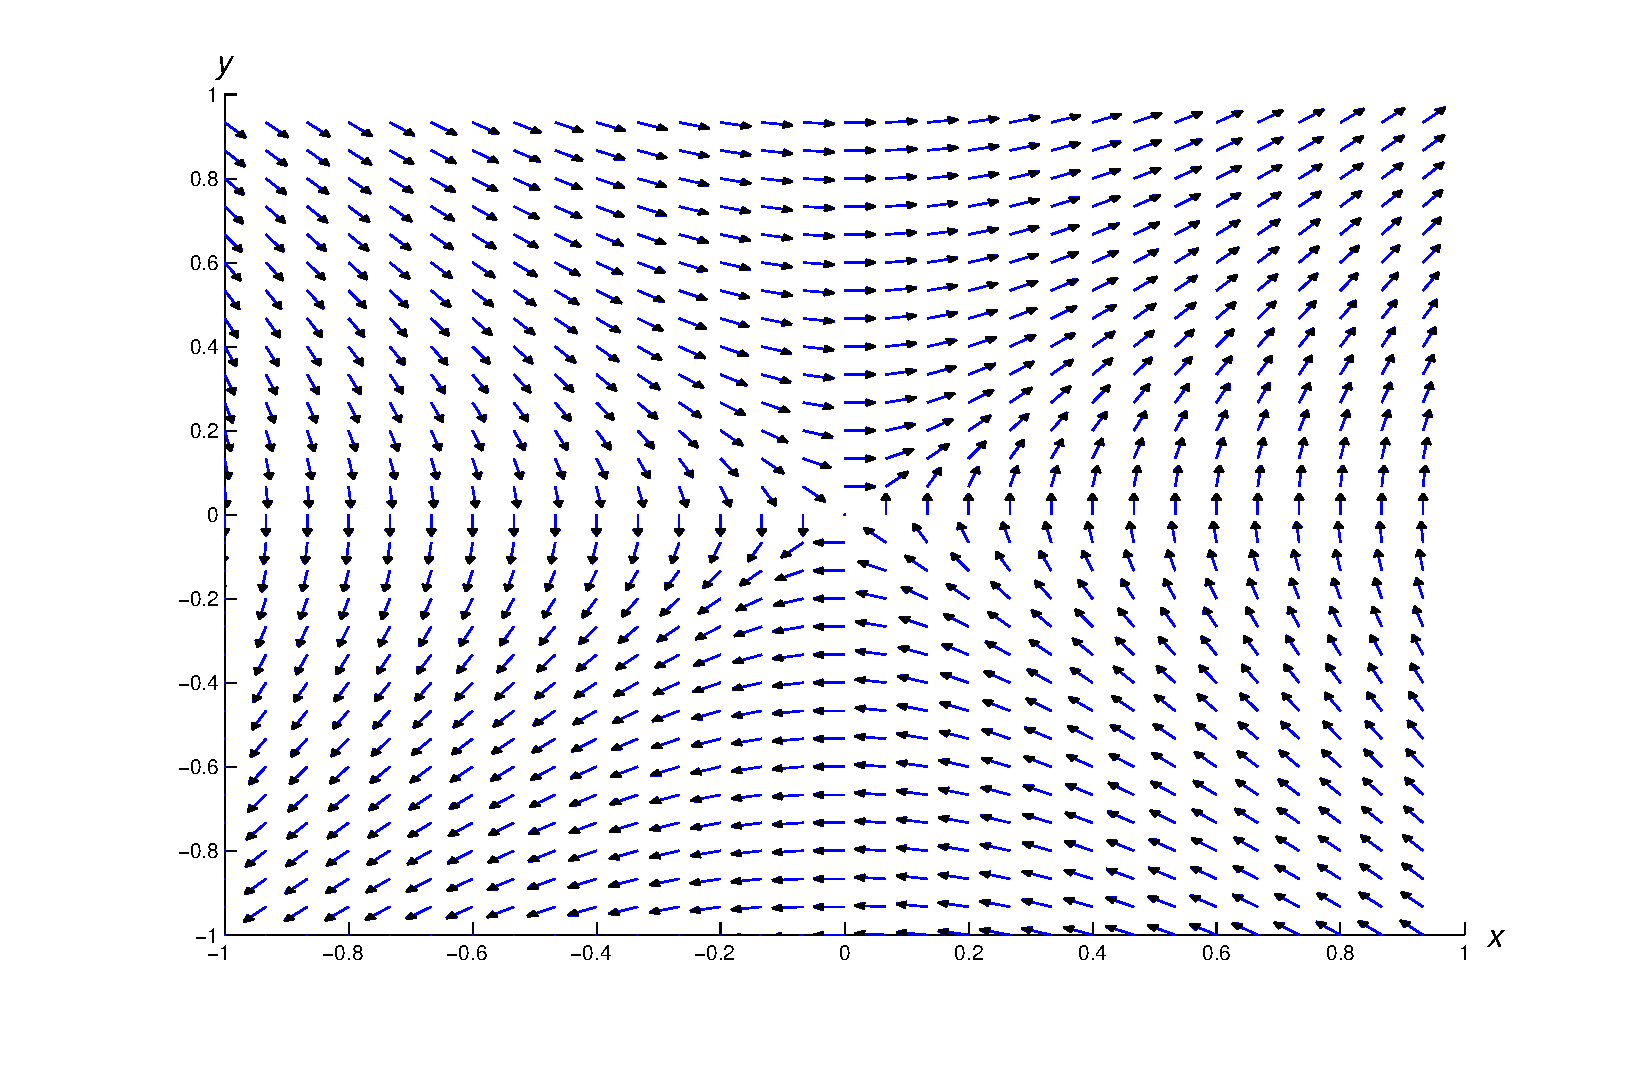
\includegraphics[bb=-78 148 689 643,width=5.67in,height=3.66in,keepaspectratio]{exer010301}
  \caption*{{\color{red}\bf 1}\; A direction field for
$y'=\dst{\frac{x}{y}}$}
\end{figure}


\newpage


\begin{figure}[H]
  \color{blue}
  \centering
  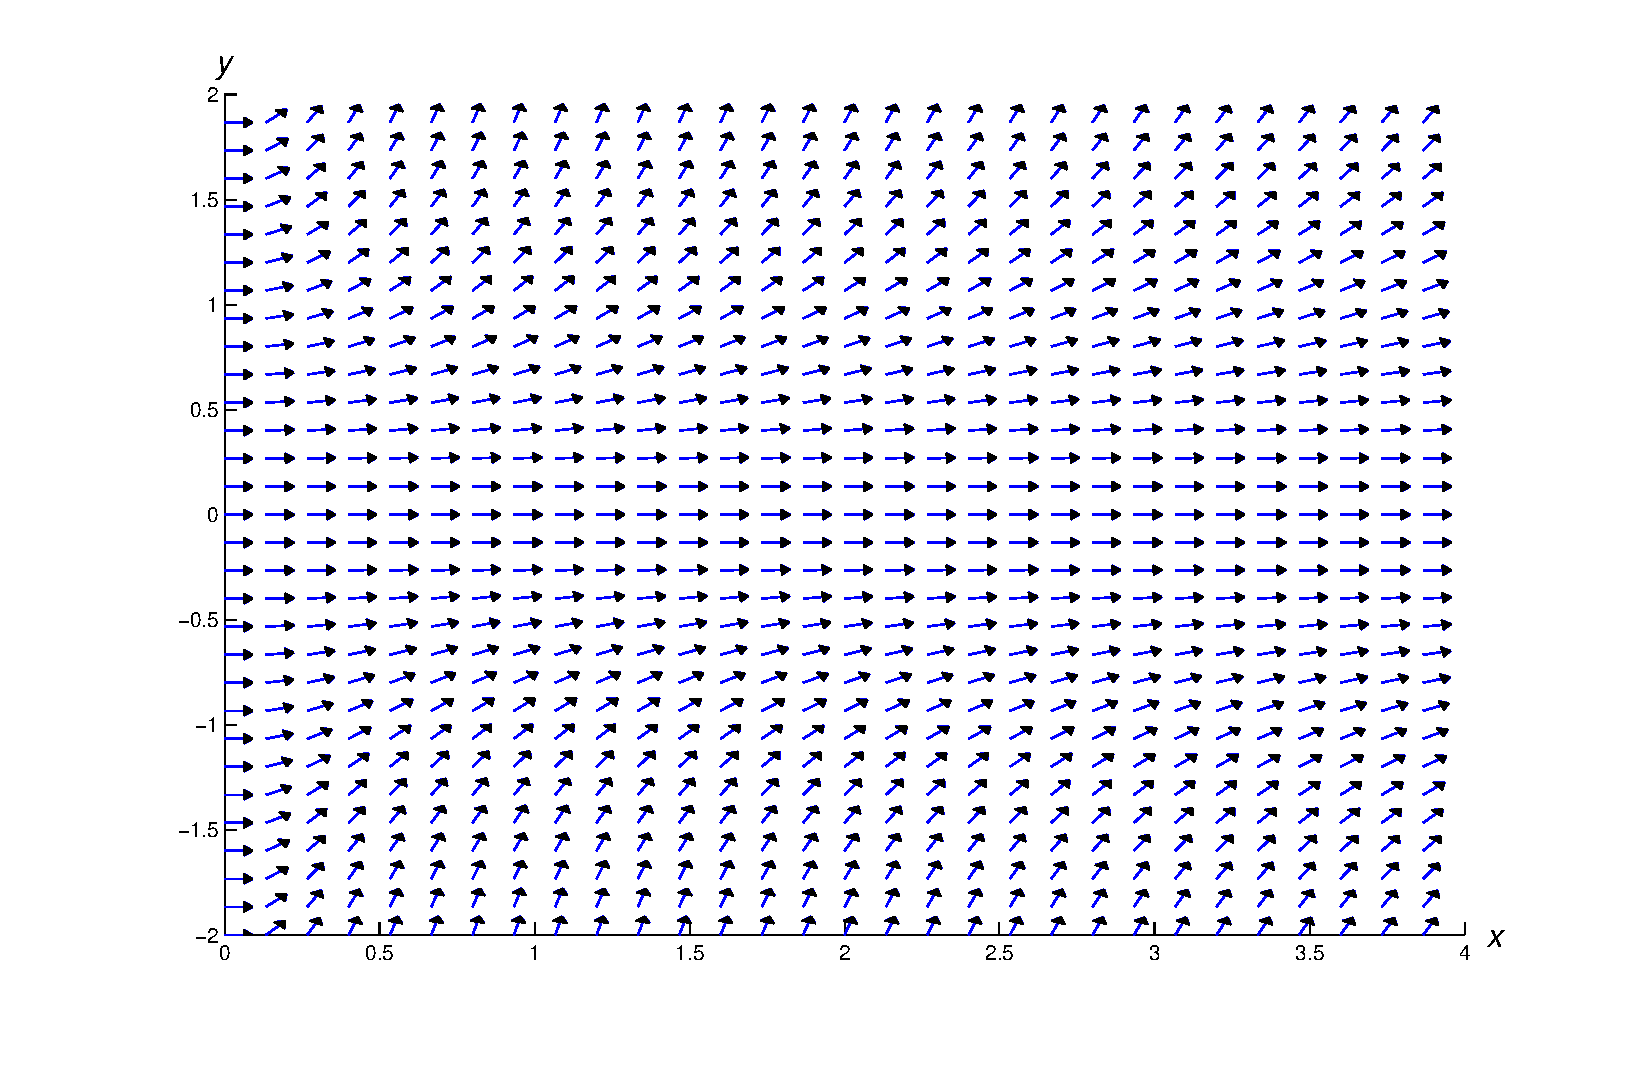
\includegraphics[bb=-78 148 689 643,width=5.67in,height=3.66in,keepaspectratio]{exer010302}
  \caption*{{\color{red}\bf 2}\; A direction field for
 $\dst{y'=\dst{2xy^2\over1+x^2}}$\quad}
\end{figure}






\begin{figure}[H]
  \color{blue}
  \centering
  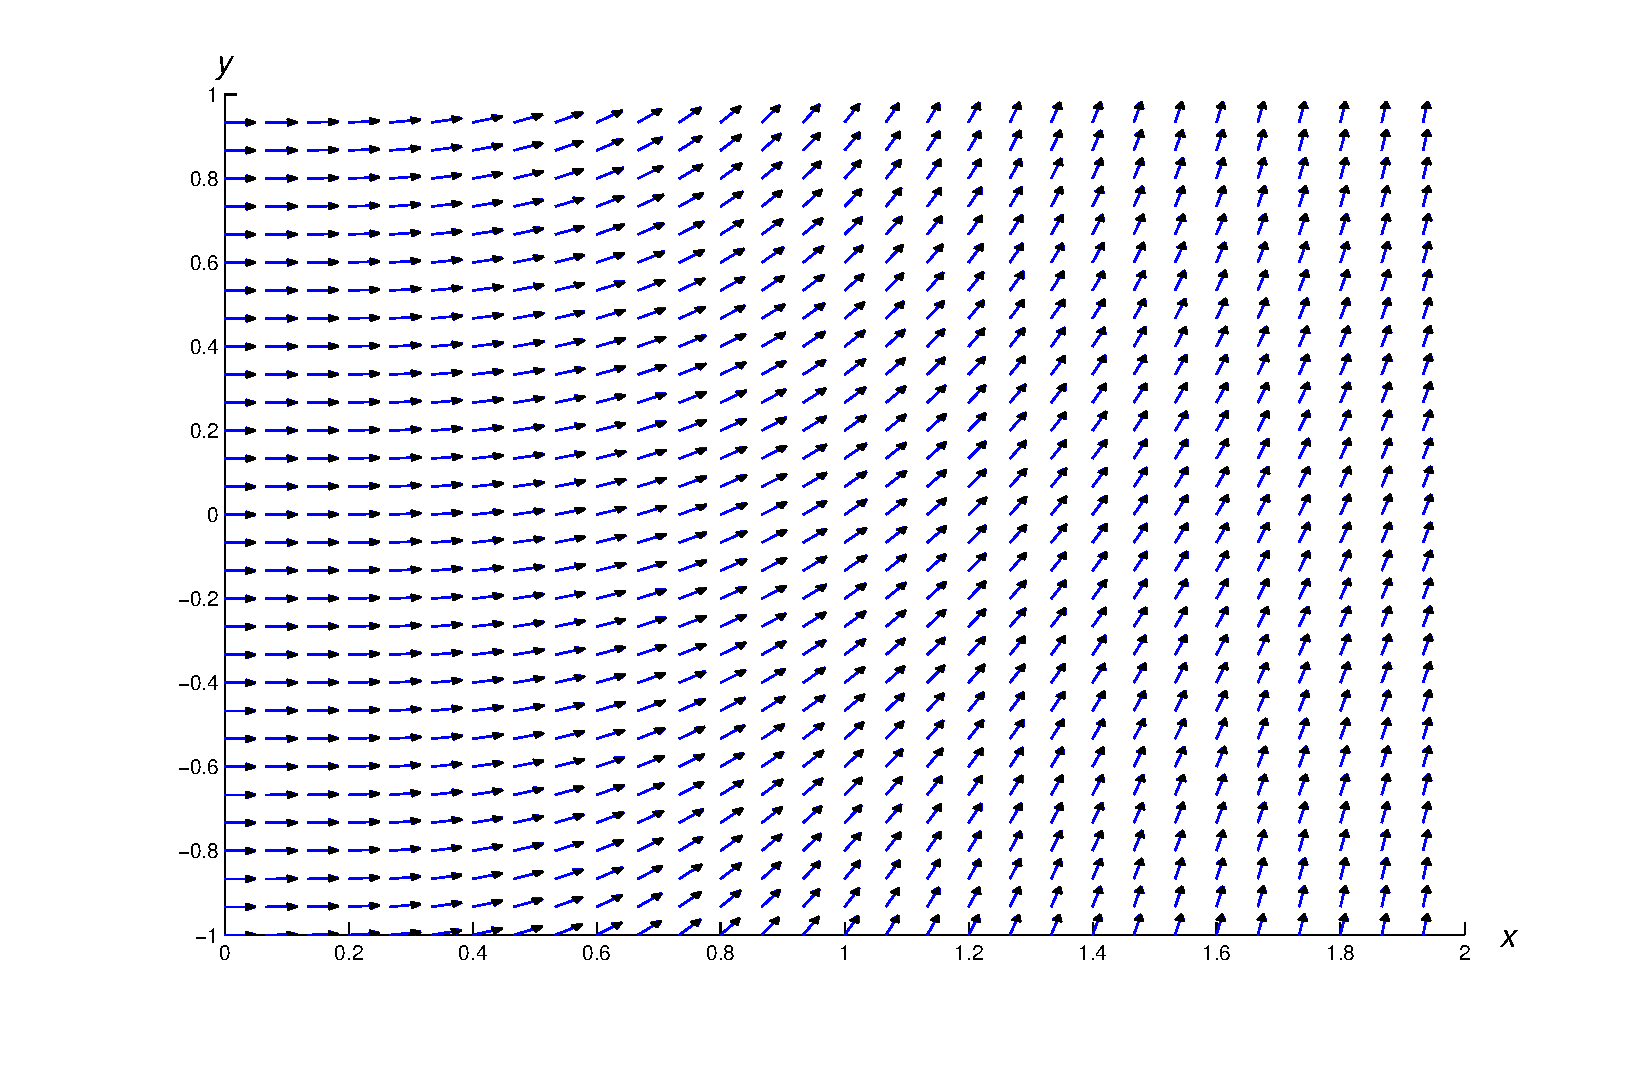
\includegraphics[bb=-78 148 689 643,width=5.67in,height=3.66in,keepaspectratio]{exer010303}
  \caption*{{\color{red}\bf 3}\; A direction field for
 $y'=x^2(1+y^2)$}
\end{figure}



\begin{figure}[H]
  \color{blue}
  \centering
  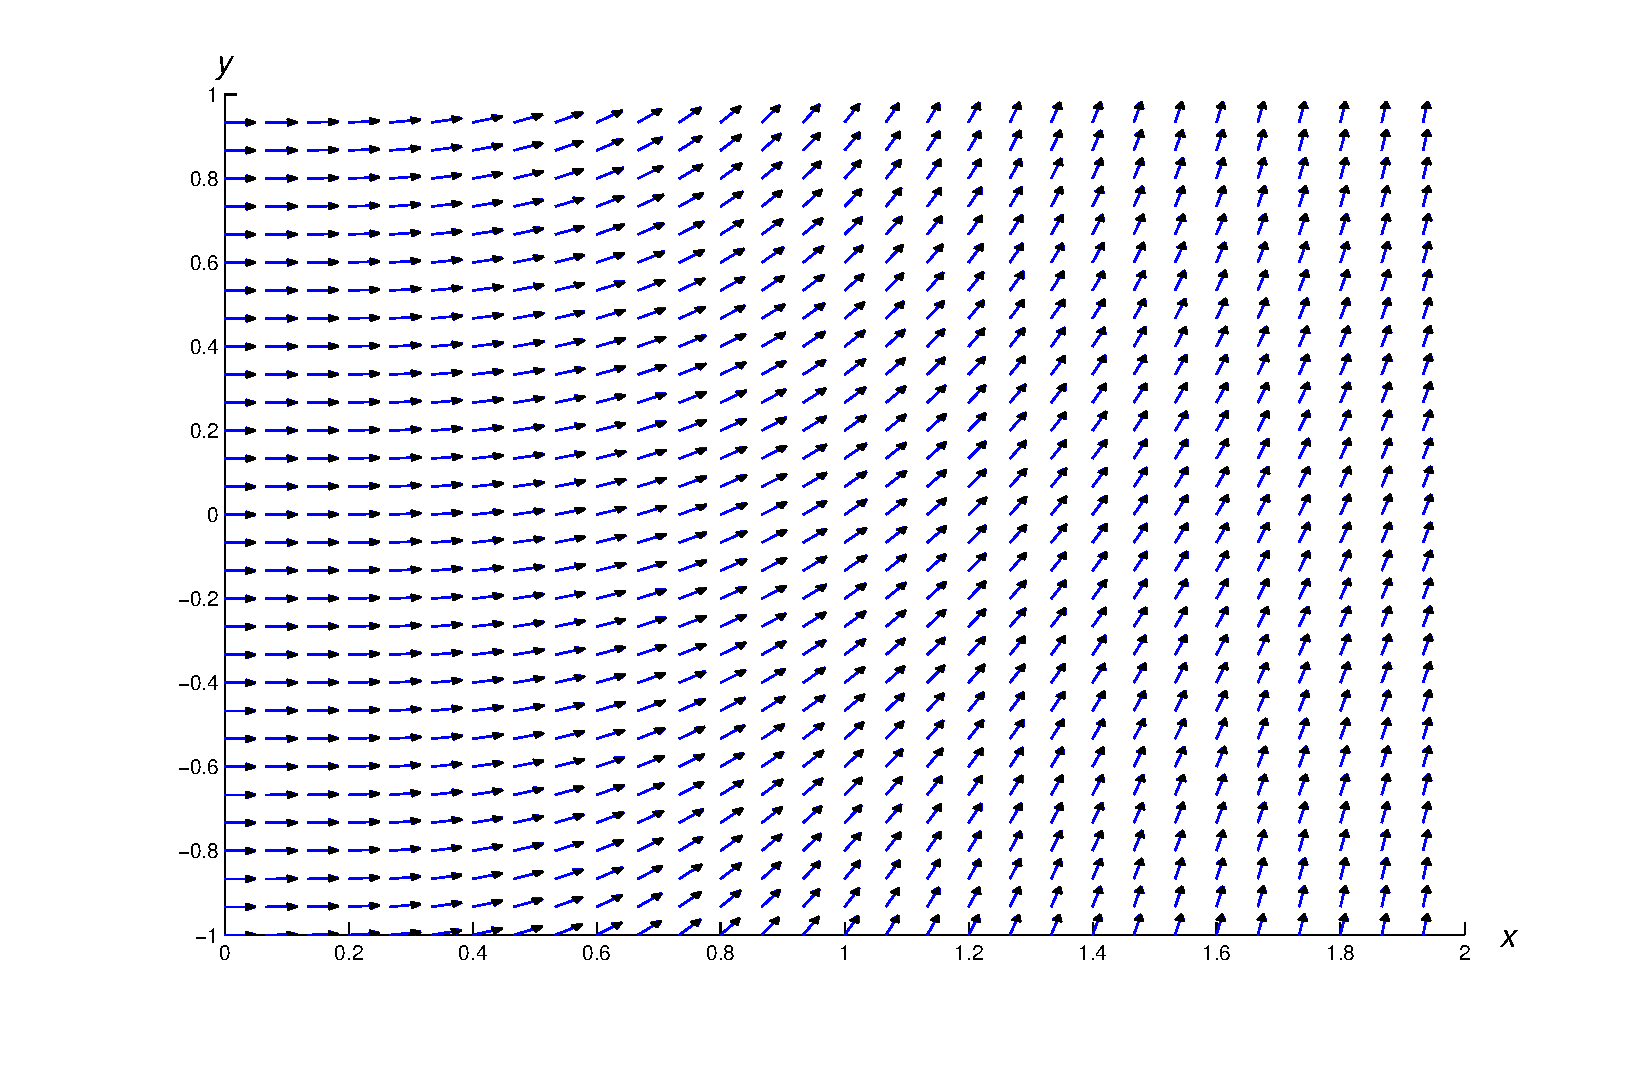
\includegraphics[bb=-78 148 689 643,width=5.67in,height=3.66in,keepaspectratio]{exer010304}
  \caption*{{\color{red}\bf 4}\; A direction field for
$y'=\dst{1\over1+x^2+y^2}$}
\end{figure}



\begin{figure}[H]
  \color{blue}
  \centering
  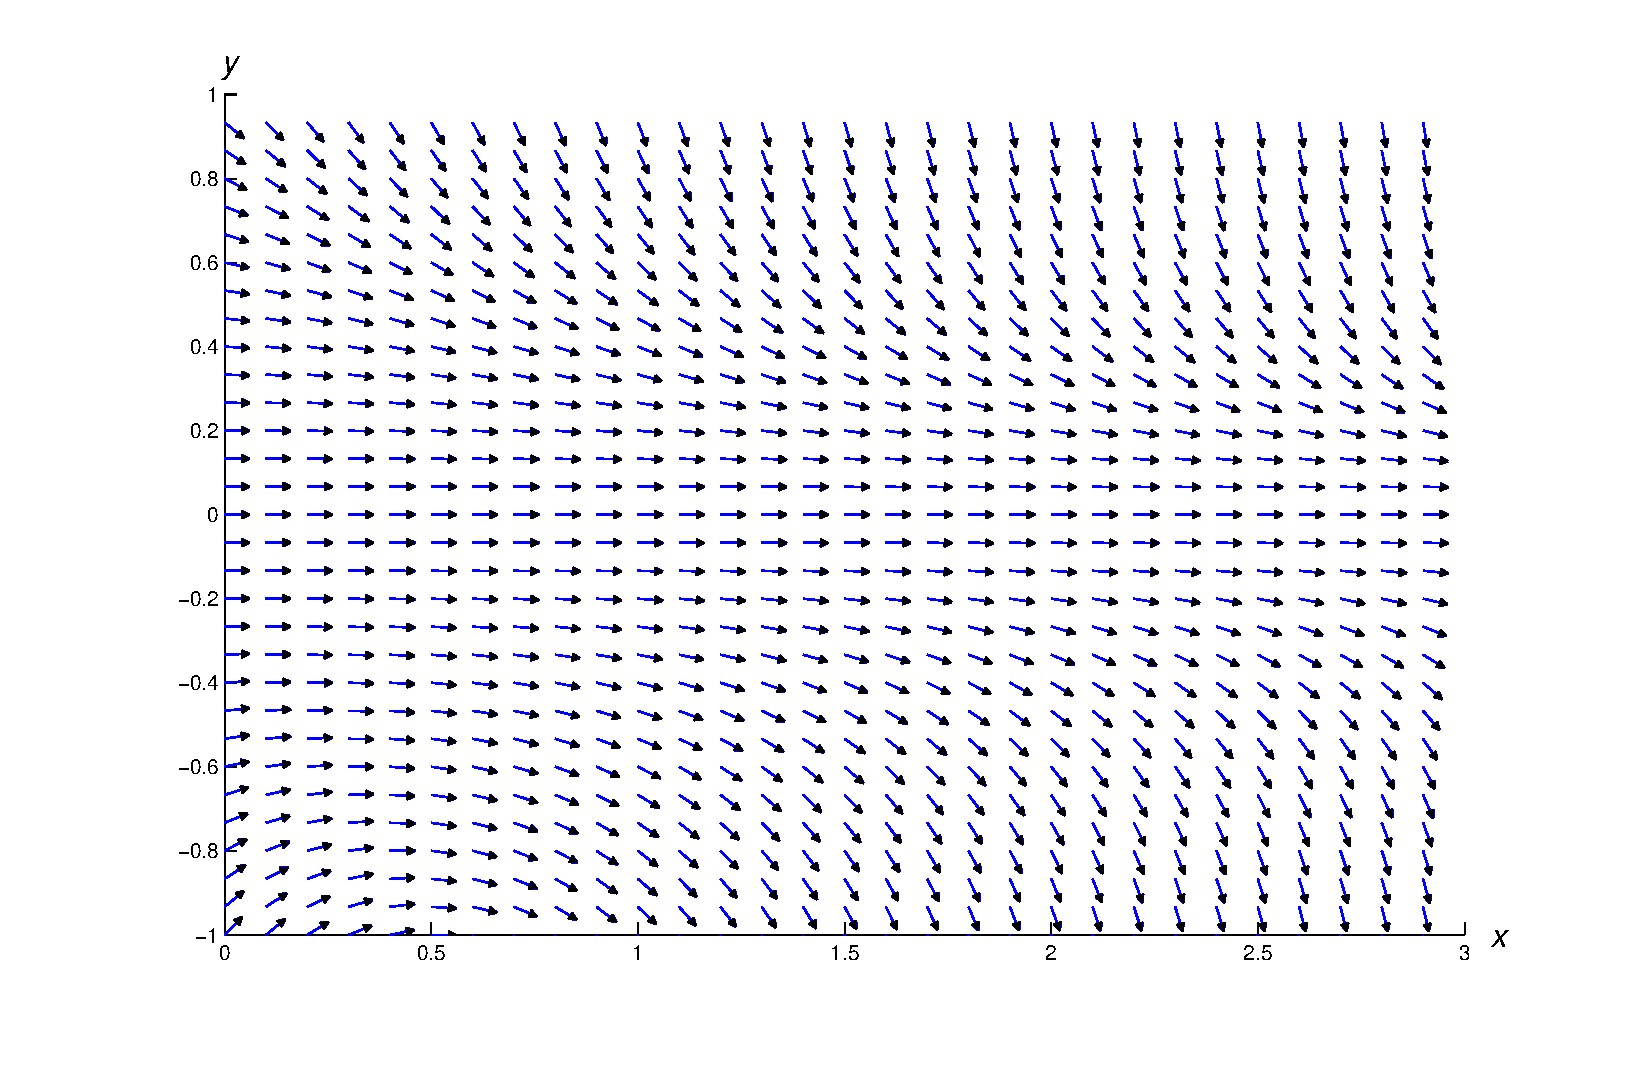
\includegraphics[bb=-78 148 689 643,width=5.67in,height=3.66in,keepaspectratio]{exer010305}
  \caption*{{\color{red}\bf 5}\; A direction field for
$y'=-(2xy^2+y^3)$}
\end{figure}



\begin{figure}[H]
  \color{blue}
  \centering
  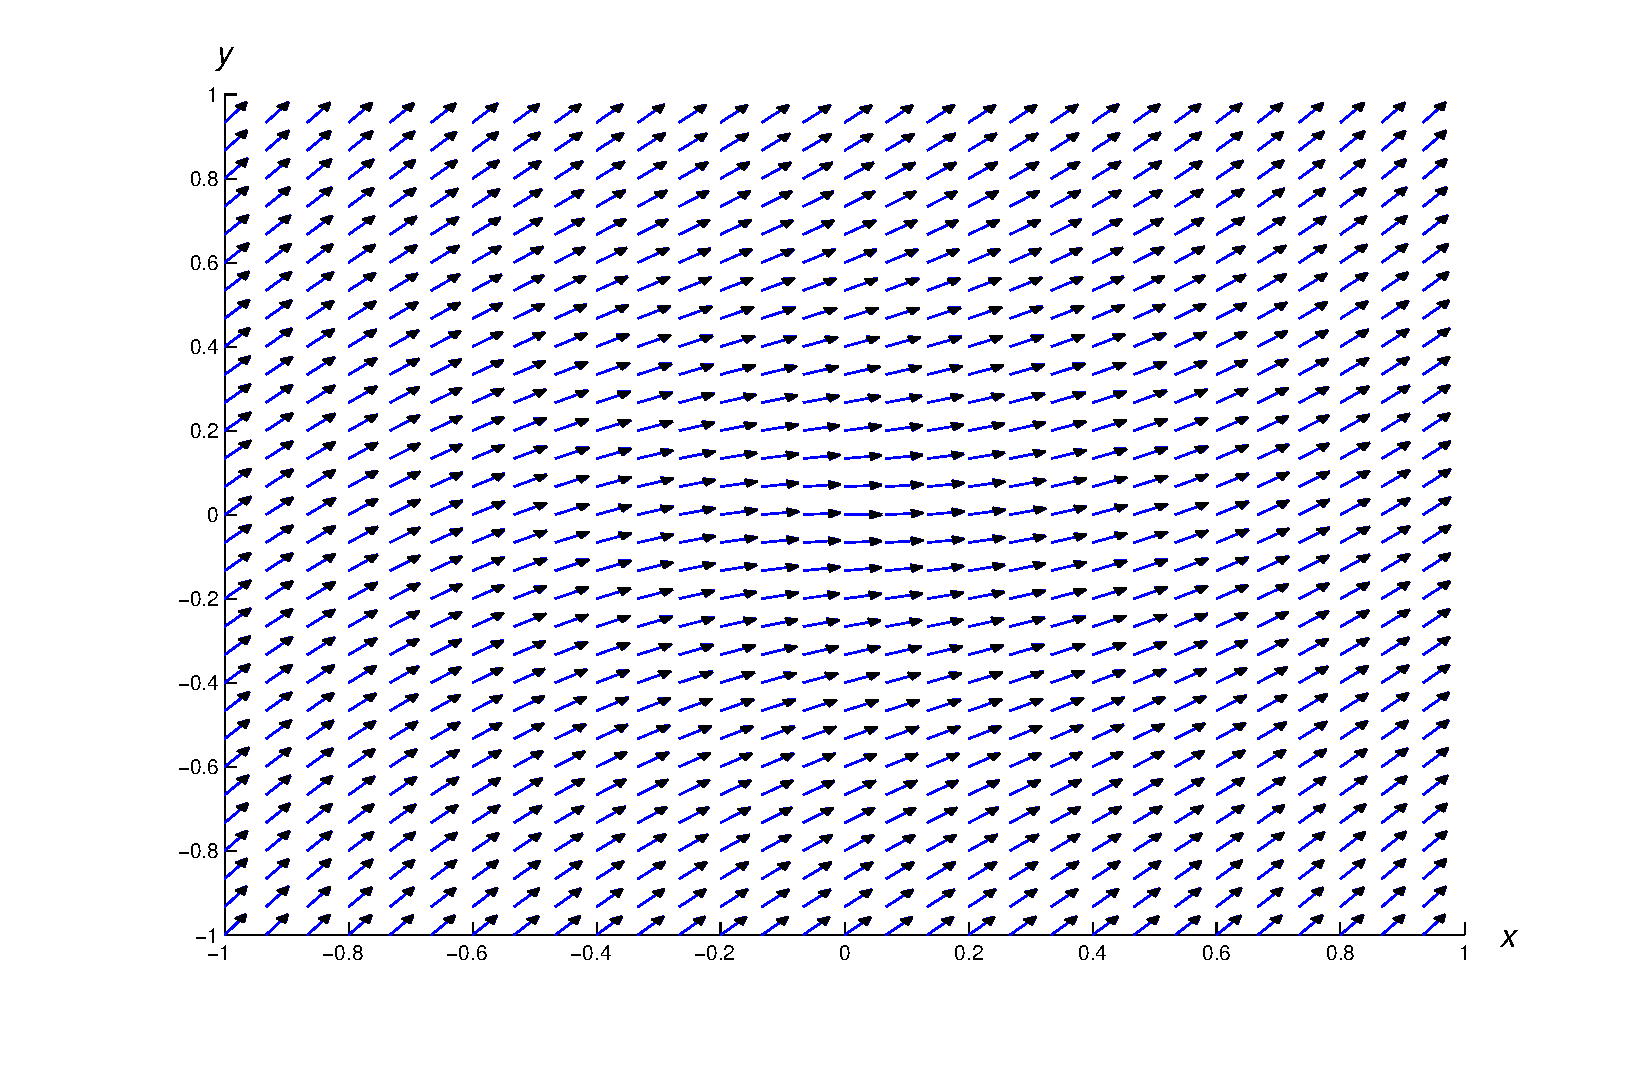
\includegraphics[bb=-78 148 689 643,width=5.67in,height=3.66in,keepaspectratio]{exer010306}
  \caption*{{\color{red}\bf 6}\; A direction field for
$y'=(x^2+y^2)^{1/2}$}
\end{figure}



\begin{figure}[H]
  \color{blue}
  \centering
  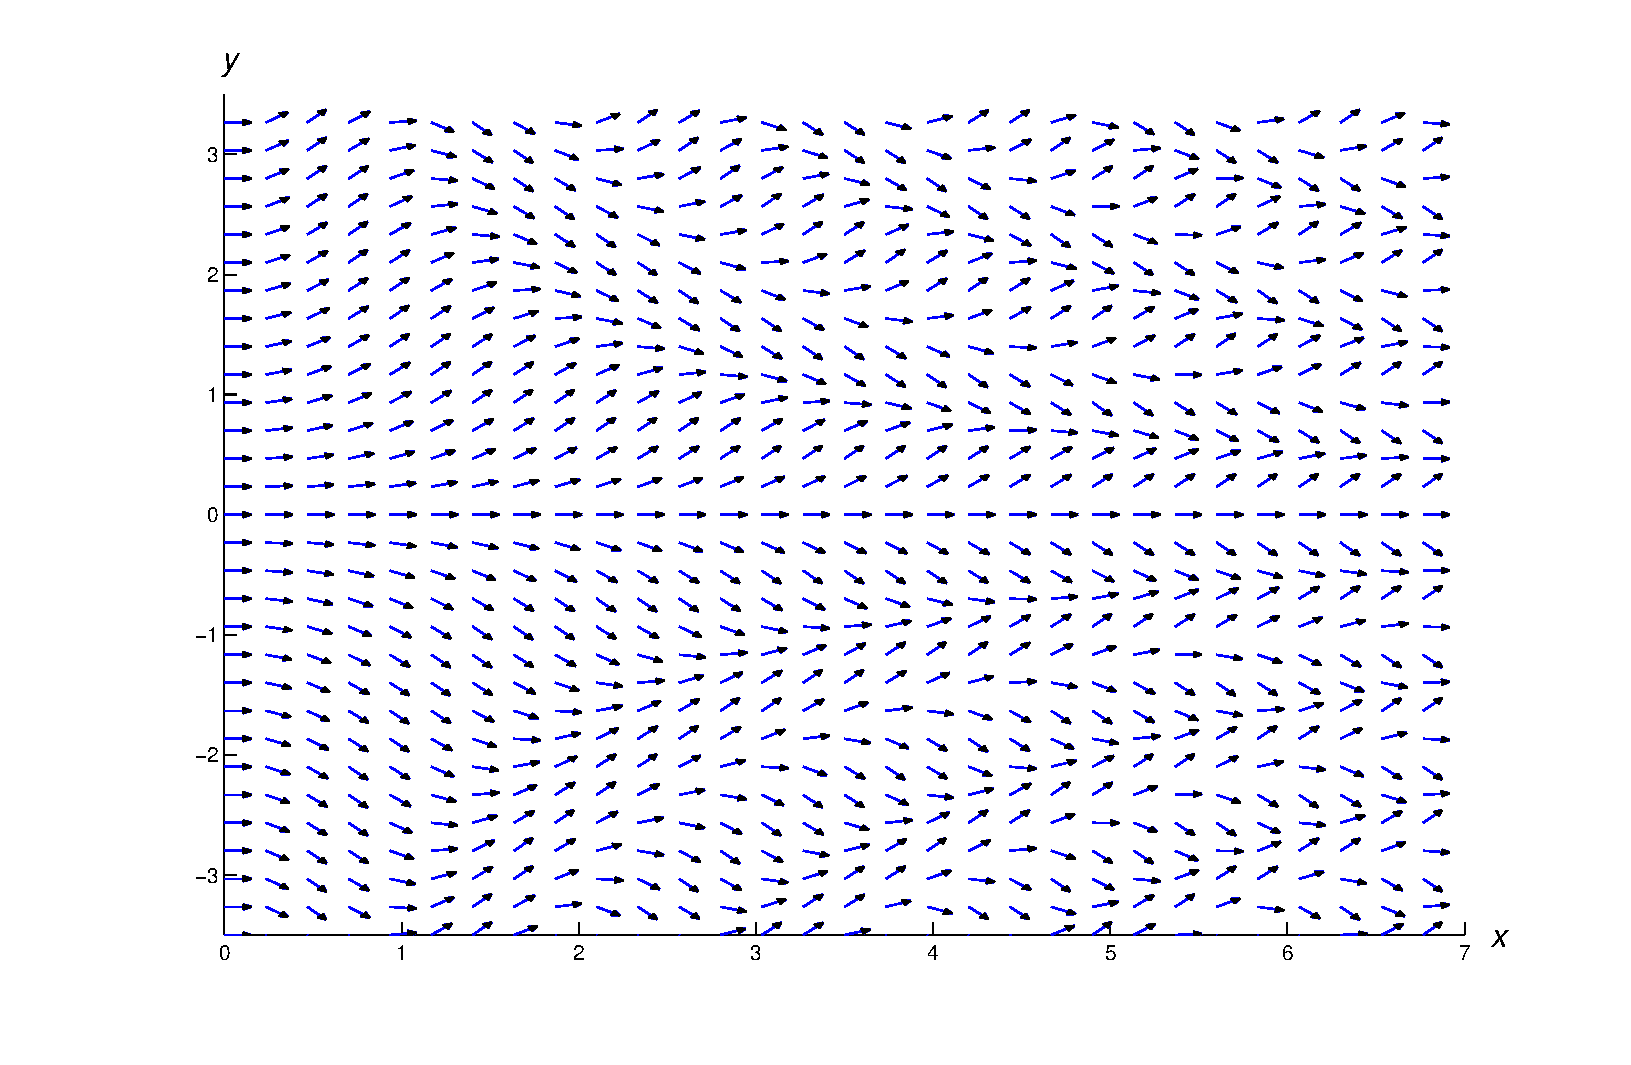
\includegraphics[bb=-78 148 689 643,width=5.67in,height=3.66in,keepaspectratio]{exer010307}
  \caption*{{\color{red}\bf 7}\; A direction field for
$y'=\sin xy$}
\end{figure}



\begin{figure}[H]
  \color{blue}
  \centering
  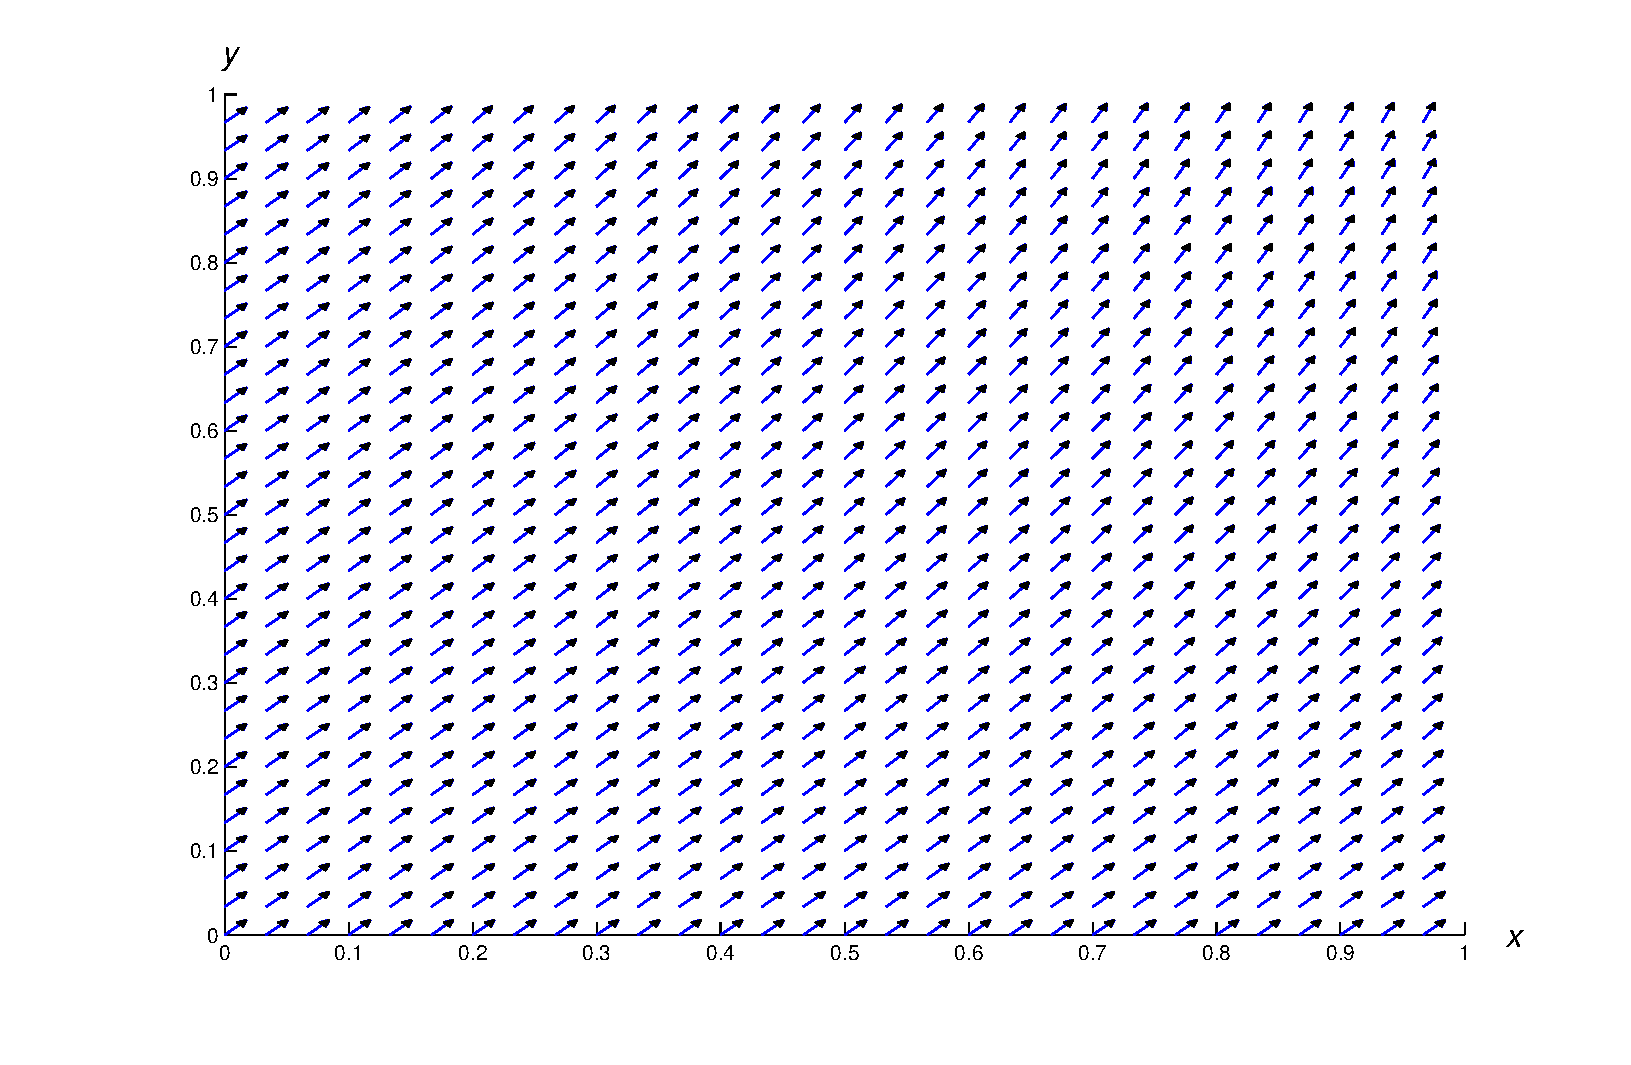
\includegraphics[bb=-78 148 689 643,width=5.67in,height=3.66in,keepaspectratio]{exer010308}
  \caption*{{\color{red}\bf 8}\; A direction field for
 $y'=e^{xy}$}
\end{figure}



\begin{figure}[H]
  \color{blue}
  \centering
  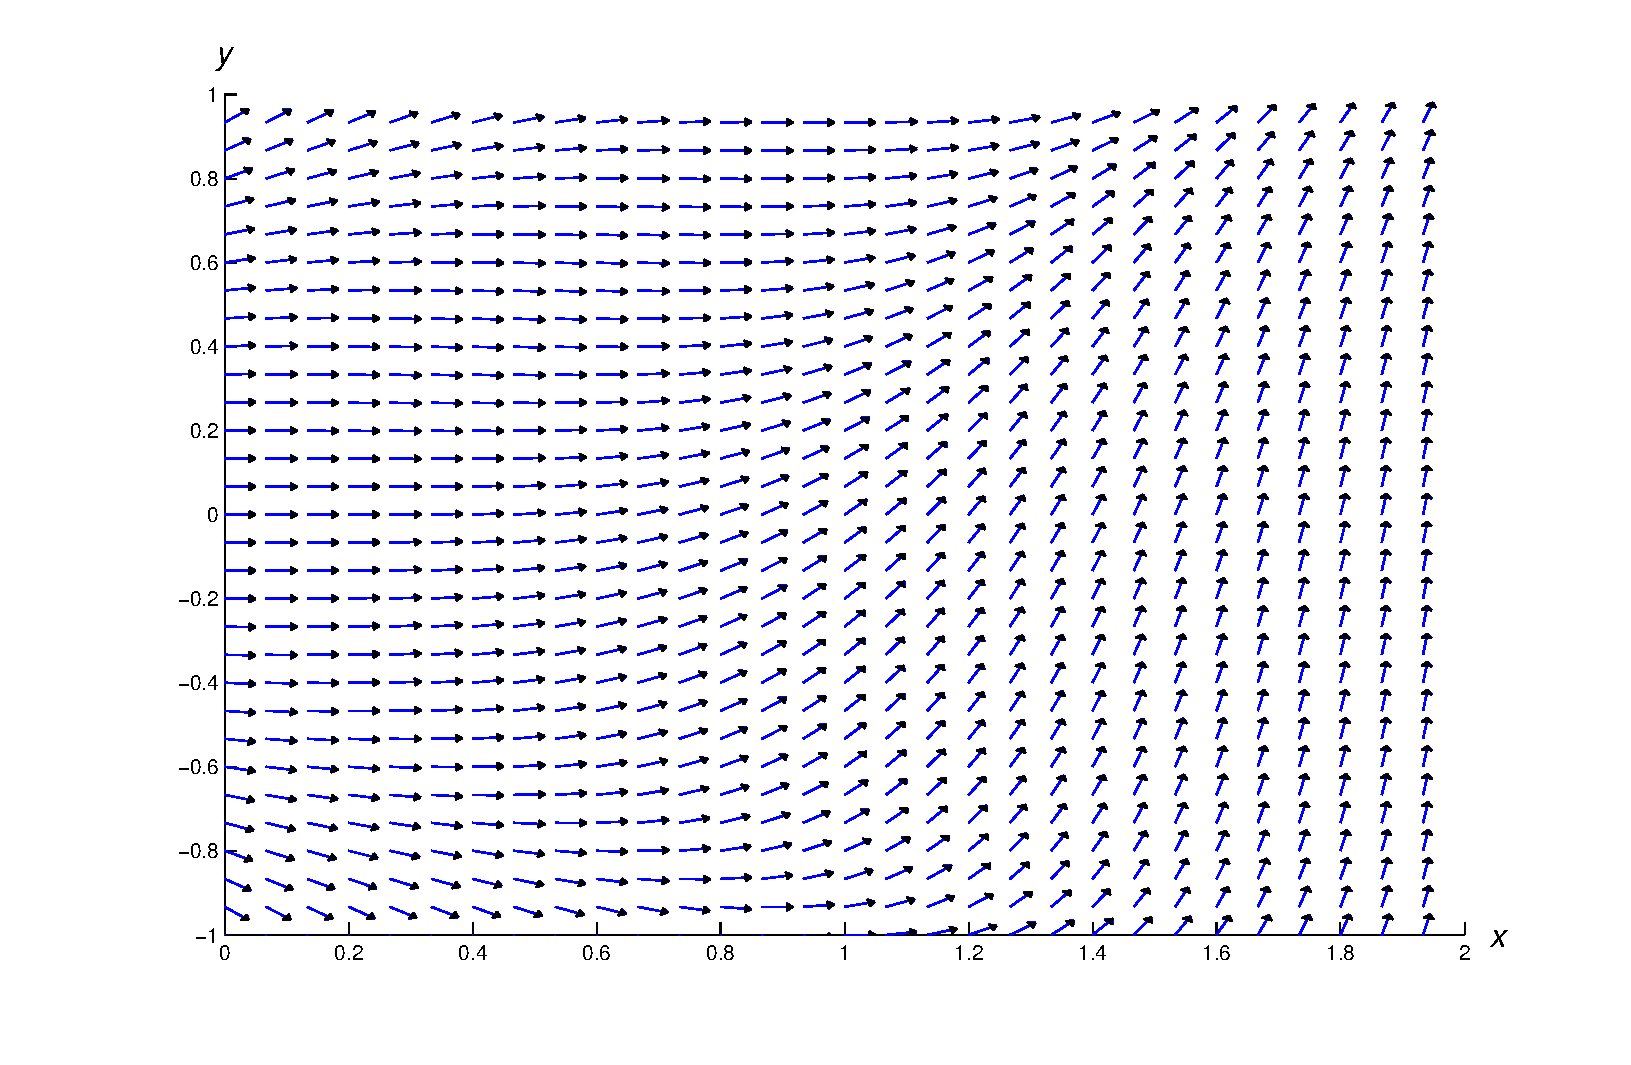
\includegraphics[bb=-78 148 689 643,width=5.67in,height=3.66in,keepaspectratio]{exer010309}
  \caption*{{\color{red}\bf 9}\; A direction field for
$y'=(x-y^2)(x^2-y)$}
\end{figure}



\begin{figure}[H]
  \color{blue}
  \centering
  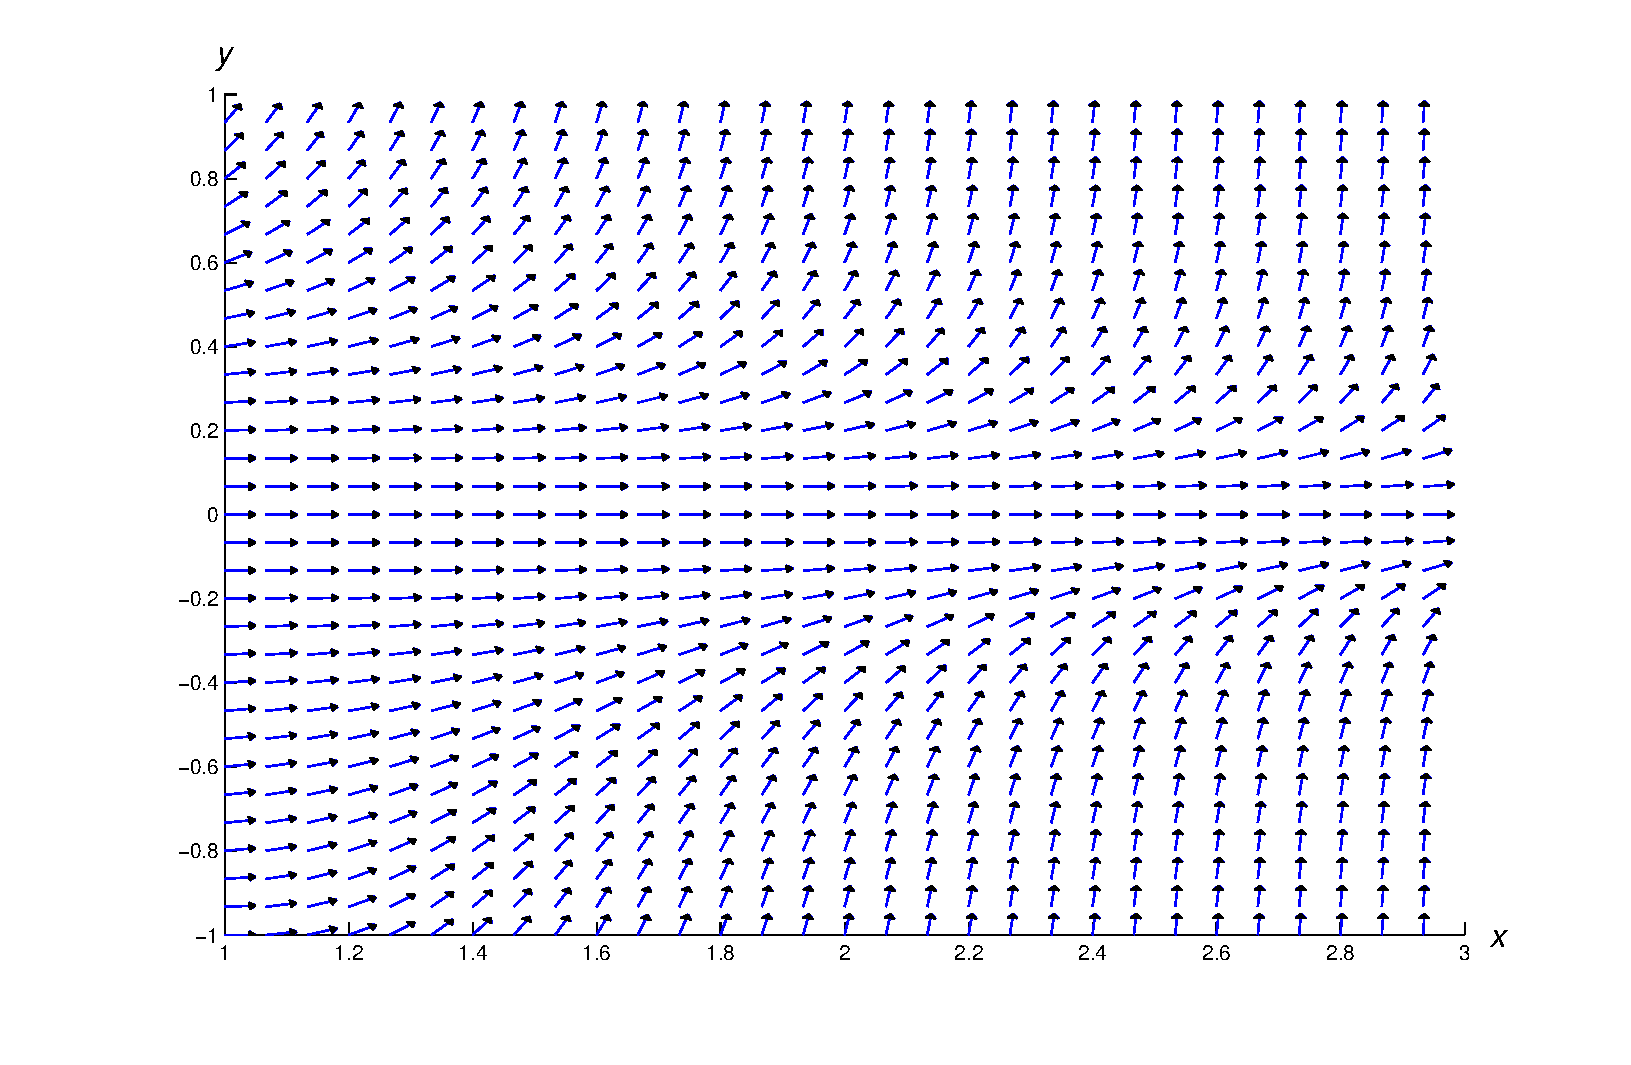
\includegraphics[bb=-78 148 689 643,width=5.67in,height=3.66in,keepaspectratio]{exer010310}
  \caption*{{\color{red}\bf 10}\; A direction field for
$y'=x^3y^2+xy^3$}
\end{figure}



\begin{figure}[H]
  \color{blue}
  \centering
  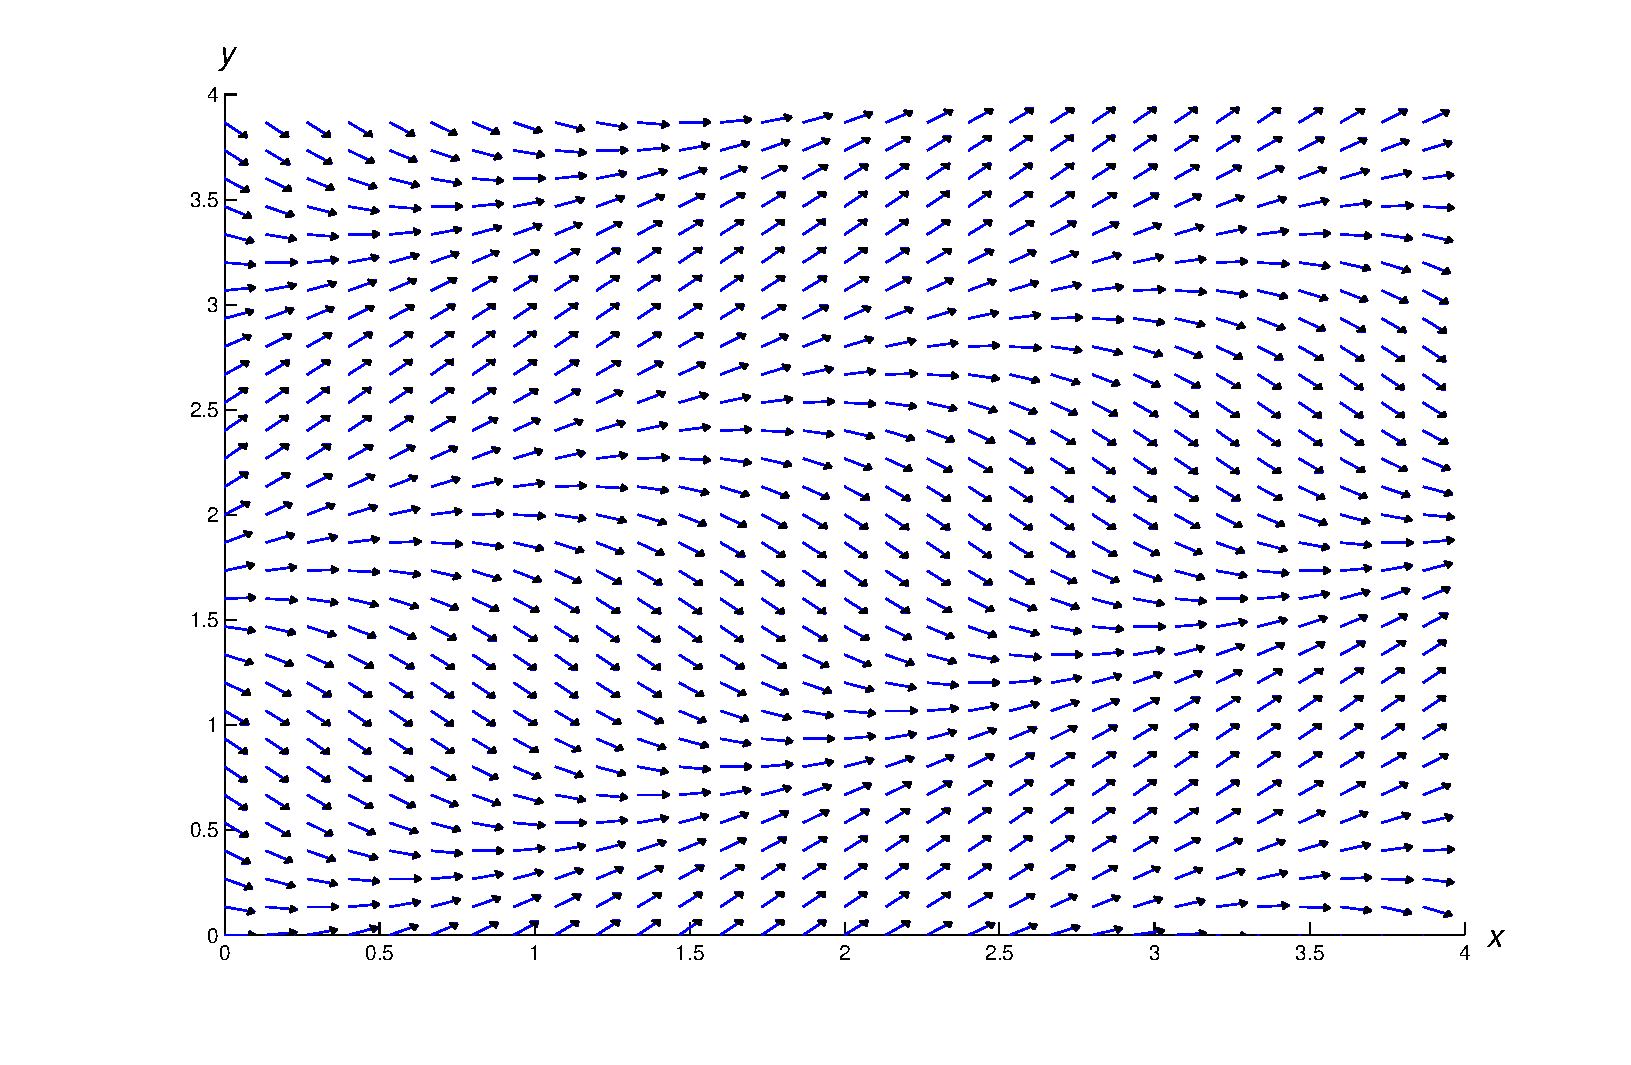
\includegraphics[bb=-78 148 689 643,width=5.67in,height=3.66in,keepaspectratio]{exer010311}
  \caption*{{\color{red}\bf 11}\; A direction field for
$y'=\sin(x-2y)$}
\end{figure}

\newpage
\emph{In Exercises~\ref{exer:1.3.12}-\ref{exer:1.3.22} construct a
direction
field and plot some integral curves in the indicated rectangular region.}


\begin{exerciselist}
\setcounter{exercise}{11}
\item\label{exer:1.3.12}\CGex
$y'=y(y-1);    \quad  \{-1\le x\le 2,\ -2\le y\le2\}$

\item\label{exer:1.3.13} \CGex
$y'=2-3xy;    \quad  \{-1\le x\le 4,\ -4\le y\le4\}$

\item\label{exer:1.3.14} \CGex
$y'=xy(y-1);    \quad  \{-2\le x\le2,\ -4\le y\le 4\}$

\item\label{exer:1.3.15}\CGex
$y'=3x+y;    \quad  \{-2\le x\le2,\ 0\le y\le 4\}$

\item\label{exer:1.3.16} \CGex
$y'=y-x^3;    \quad  \{-2\le x\le2,\ -2\le y\le 2\}$

\item\label{exer:1.3.17}\CGex
$y'=1-x^2-y^2;    \quad  \{-2\le x\le2,\ -2\le y\le 2\}$

\item\label{exer:1.3.18}\CGex
$y'=x(y^2-1);    \quad  \{-3\le x\le3,\ -3\le y\le 2\}$

\item\label{exer:1.3.19}\CGex
$y'=\dst{x\over y(y^2-1)};    \quad  \{-2\le x\le2,\ -2\le y\le 2\}$

\item\label{exer:1.3.20}\CGex
$y'=\dst{xy^2\over y-1};    \quad  \{-2\le x\le2,\ -1\le y\le 4\}$

\item\label{exer:1.3.21}\CGex
$y'=\dst{x(y^2-1)\over y};    \quad  \{-1\le x\le1,\ -2\le y\le 2\}$

\item\label{exer:1.3.22}\CGex
$y'=-\dst{x^2+y^2\over1-x^2-y^2};    \quad  \{-2\le x\le2,\ -2\le y\le 2\}$


\item\label{exer:1.3.23} \Lex
By suitably renaming the constants and  dependent variables
in the equations
$$
T' = -k(T-T_m)
\eqno{\rm(A)}
$$
and
$$
G'=-\lambda G+r
\eqno{\rm(B)}
$$
discussed in Section~1.2 in connection with Newton's
law of cooling and absorption of glucose in the body, we can
write both as
$$
y'=- ay+b,
\eqno{\rm(C)}
$$
where $a$ is a positive constant and $b$ is an arbitrary
constant. Thus, (A) is of the form (C) with $y=T$, $a=k$, and
$b=kT_m$, and (B) is of the form (C) with $y=G$,
$a=\lambda$, and $b=r$. We'll encounter equations of the form
(C) in many other applications in Chapter~2.

Choose a positive  $a$  and an
arbitrary  $b$.
 Construct a  direction field and plot some integral curves for (C) in
a rectangular
region of the form
$$
\{0\le t\le T,\ c\le y\le d\}
$$
 of the $ty$-plane.
 Vary $T$, $c$, and $d$ until you discover a common property
of all the solutions of (C). Repeat this experiment with various
choices of $a$ and $b$ until you can state
this property precisely in terms of $a$ and $b$.

\item\label{exer:1.3.24} \Lex
By suitably renaming the constants and  dependent variables
in the equations
$$
P'=aP(1-\alpha P)
\eqno{\rm(A)}
$$
and
$$
I'=rI(S-I)
\eqno{\rm(B)}
$$
discussed in Section~1.1 in connection with Verhulst's
population
model and the spread of an epidemic, we can write both in the form
$$
y'=ay-by^2,
\eqno{\rm(C)}
$$
where $a$ and $b$ are positive constants. Thus, (A) is of the form (C)
with $y=P$, $a=a$, and $b=a\alpha$, and (B) is of the form (C) with
$y=I$, $a=rS$, and $b=r$. In Chapter~2 we'll encounter
equations of the form
(C) in
 other applications..

\begin{alist}
\item % (a)
Choose positive numbers $a$ and $b$. Construct a direction field and
plot some integral curves for (C) in a rectangular region of the form
$$
\{0\le t\le T,\ 0\le y\le d\}
$$
of the $ty$-plane. Vary $T$ and $d$ until you discover a common
property of all solutions of (C) with $y(0)>0$. Repeat this experiment
with various choices of $a$ and $b$ until you can state this property
precisely in terms of $a$ and $b$.

\item % (a)
Choose  positive numbers $a$ and $b$. Construct a direction field and
plot some integral curves for (C) in a rectangular region of the form
$$
\{0\le t\le T,\ c\le y\le 0\}
$$
of the $ty$-plane. Vary $a$, $b$, $T$ and $c$ until you discover a
common property of all solutions of (C) with $y(0)<0$.

You can verify your results later by doing Exercise~2.2.~\hspace*{-3pt}\ref{exer:2.2.27}.

\end{alist}
\end{exerciselist}

\newpage
\thispagestyle{empty}


\setcounter{chapter}{2}
\pdfbookmark[0]{Chapter 2 First Order Equations}{chapter:2}
\chaptertitle{First Order Equations}


\noindent
IN THIS CHAPTER we study
first order equations for which there are general methods of
solution.


\medskip\noindent
SECTION~2.1 deals with linear equations, the simplest kind
of first order equations. In this section we introduce the method of
variation of parameters. The idea underlying this method will be a
unifying theme for our approach to solving many different kinds of
differential equations throughout the book.

\medskip\noindent
SECTION~2.2 deals with separable equations, the simplest
nonlinear equations. In this section we introduce the idea of implicit
and constant solutions of differential equations, and we point out
some differences between the properties of linear and nonlinear
equations.

\medskip\noindent
SECTION~2.3 discusses existence and
uniqueness of solutions of nonlinear equations. Although it may seem
logical to place this section before Section~2.2, we
presented
Section~2.2 first so we could have illustrative examples in
Section~2.3.

\medskip\noindent
SECTION~2.4 deals with nonlinear equations that are not
separable, but can be transformed into separable equations by a
procedure similar to variation of parameters.


\medskip\noindent
SECTION~2.5 covers exact differential equations, which are
given this name because the method for solving them uses the idea of
an exact differential from calculus.


\medskip\noindent
SECTION~2.6 deals with
equations that are not exact, but can made exact by multiplying them
by a function known called {\color{blue}\it integrating factor\/}.




\centerline{29}
\newpage


\subpdfbookmark{Section 2.1 Linear First Order Equations} {section:2.1}
\setcounter{section}{1}
\renewcommand{\thissection}
{\sectiontitle{\,LINEAR FIRST ORDER EQUATIONS}}
\thissection

\newsection{1}{First Order Equations}{Linear First Order Equations}


\noindent
A first order differential equation is said to be {\color{blue}\it linear\/} if it
can be written as

\begin{equation}\label{eq:2.1.1}
y'+p(x)y=f(x).
\end{equation}
A first order differential equation that can't be written like this
is {\color{blue}\it nonlinear\/}. We say that \eqref{eq:2.1.1} is {\color{blue}\it homogeneous\/}
if $f\equiv0$;     otherwise it's {\color{blue}\it nonhomogeneous\/}. Since
$y\equiv0$ is obviously a solution of the homgeneous equation
$$
y'+p(x)y=0,
$$
we call it the {\color{blue}\it trivial solution\/}. Any  other solution
is {\color{blue}\it nontrivial\/}.


\begin{example}\label{example:2.1.1}\rm
 The first order equations
\begin{eqnarray*}
x^2y'+3y&=&x^2,\\[2\jot]
xy'-8x^2y&=&\sin x,\\
xy'+(\ln x)y&=&0,\\
y'&=&x^2y - 2,
\end{eqnarray*}
are not in the form \eqref{eq:2.1.1}, but they are linear, since they can
be rewritten as
\begin{eqnarray*}
y'+{3\over x^2}y&=&1,\\
y'-8xy&=&{\sin x\over x},\\
y'+{\ln x\over x}y&=&0,\\
y'-x^2y&=&-2.
\end{eqnarray*}
\end{example}


\begin{example}\label{example:2.1.2}\rm
Here are some
nonlinear first order equations:
$$
\begin{array}{rcrc}
xy'+3y^2 & =& 2x&\qquad\mbox{(because $y$ is squared)},\\[2\jot]
yy'& =&3&\qquad\mbox{(because of the product $yy'$)},\\[2\jot]
y'+xe^y &=&12&\qquad\mbox{(because of $e^y$)}.
\end{array}
$$
\end{example}

\boxit{General Solution of a Linear First Order Equation}


\noindent
To motivate a definition that we'll need, consider the
simple linear first order equation
\begin{equation}\label{eq:2.1.2}
y'={1\over x^2}.
\end{equation}
From calculus we know that $y$ satisfies this equation
if and only if
\begin{equation}\label{eq:2.1.3}
y=-{1\over x}+c,
\end{equation}
where $c$ is an arbitrary constant.
We call $c$ a
{\color{blue}\it parameter\/} and say that \eqref{eq:2.1.3} defines a {\color{blue}\it
one--parameter family\/} of functions. For each real number $c$, the
function defined by \eqref{eq:2.1.3} is a solution of \eqref{eq:2.1.2}
on $(-\infty,0)$ and $(0,\infty)$;     moreover, every solution of
\eqref{eq:2.1.2} on either of these intervals is of the form
\eqref{eq:2.1.3} for some choice of $c$. We say that \eqref{eq:2.1.3}
is {\color{blue}\it the general solution\/} of~\eqref{eq:2.1.2}.

We'll  see that a similar situation occurs in connection with any
first order linear equation
\begin{equation}\label{eq:2.1.4}
y'+p(x)y=f(x);
\end{equation}
that is, if $p$ and $f$ are continuous on some open interval $(a,b)$ then
 there's a unique formula $y=y(x,c)$ analogous to \eqref{eq:2.1.3}
that involves $x$ and a parameter $c$ and has  the these
properties:
\begin{itemize}
\item % ()
For each fixed value of $c$, the resulting function of $x$ is a
solution of \eqref{eq:2.1.4} on $(a,b)$.
\item % ()
If $y$ is a solution of \eqref{eq:2.1.4} on $(a,b)$, then $y$ can be
obtained from the formula by choosing $c$ appropriately.
\end{itemize}
We'll call $y=y(x,c)$ the {\color{blue}\it general solution\/} of
\eqref{eq:2.1.4}.

When this has been established, it will follow that
an equation of the form
\begin{equation}\label{eq:2.1.5}
P_0(x)y'+P_1(x)y=F(x)
\end{equation}
has a general solution on  any open interval $(a,b)$ on which $P_0$,
$P_1$, and $F$ are all continuous and $P_0$ has no zeros, since in
this case we can rewrite \eqref{eq:2.1.5} in the form \eqref{eq:2.1.4}
with $p=P_1/P_0$ and $f=F/P_0$, which are both continuous on $(a,b)$.

To avoid awkward wording in examples and exercises, we won't specify
the interval $(a,b)$ when we ask for the general solution of a
specific linear first order equation. Let's agree that this always
means that we want the general solution on every open interval on
which $p$ and $f$ are continuous if the equation is of the form
\eqref{eq:2.1.4}, or on which $P_0$, $P_1$, and $F$ are continuous and
$P_0$ has no zeros, if the equation is of the form \eqref{eq:2.1.5}. We
leave it to you to identify these intervals in specific examples and
exercises.


For completeness, we point out that if $P_0$, $P_1$, and $F$ are all
continuous on an open interval $(a,b)$, but $P_0$ {\color{blue}\it does\/} have a
zero in $(a,b)$, then \eqref{eq:2.1.5} may fail to have a general
solution on $(a,b)$ in the sense just defined. Since this isn't  a
major point that needs to be developed in depth, we won't discuss it
further;     however, see Exercise~\ref{exer:2.1.44} for
an example.

\boxit{Homogeneous Linear First Order Equations}

\noindent
We begin with the problem of finding the general solution of
a homogeneous linear first order equation.
The next example recalls a familiar result from calculus.


\begin{example}\label{example:2.1.3} \rm
   Let $a$ be a constant.
\begin{alist}
\item %(a)
Find the general solution of
\begin{equation}
y'-ay=0.\label{eq:2.1.6}
\end{equation}

\item %(b)
Solve the initial value problem
$$
y'-ay=0,\quad y(x_0)=y_0.
$$
\end{alist}
\end{example}


\solutionpart{a}
You already know from calculus that if $c$ is any constant, then
$y=ce^{ax}$ satisfies \eqref{eq:2.1.6}. However, let's pretend  you've
forgotten this, and use this problem to illustrate a general method
for solving a homogeneous linear first order equation.

We know that \eqref{eq:2.1.6} has the trivial solution $y\equiv0$. Now
suppose   $y$ is a nontrivial solution of \eqref{eq:2.1.6}. Then, since
a differentiable function must be continuous, there must be some open
interval $I$ on which $y$ has no zeros. We rewrite \eqref{eq:2.1.6} as
$$
{y'\over y}=a
$$
for $x$ in $I$. Integrating this shows that
$$
\ln|y|=ax+k,\mbox{\quad so \quad} |y|=e^ke^{ax},
$$
where $k$ is an arbitrary constant. Since $e^{ax}$ can never equal
zero,  $y$ has no zeros, so $y$ is either always
positive or always negative. Therefore we can rewrite $y$ as
\begin{equation}\label{eq:2.1.7}
y=ce^{ax}
\end{equation}
where
$$
c=\left\{\begin{array}{cl}\phantom{-}e^k&\mbox{if } y>0,
\\ -e^k&\mbox{if } y<0.\end{array}\right.
$$
This shows that every nontrivial solution of \eqref{eq:2.1.6} is of the
form $y=ce^{ax}$ for some nonzero constant $c$. Since setting $c=0$
yields the trivial solution,  {\color{blue}\it all\/} solutions of
\eqref{eq:2.1.6} are of the form \eqref{eq:2.1.7}. Conversely,
\eqref{eq:2.1.7} is a solution of \eqref{eq:2.1.6} for every choice of $c$,
since differentiating \eqref{eq:2.1.7} yields $y'=ace^{ax}=ay$.

\solutionpart{b}   Imposing  the initial condition $y(x_0)=y_0$
yields $y_0=ce^{ax_0}$, so $c=y_0e^{-ax_0}$ and
$$
y=y_0e^{-ax_0}e^{ax}=y_0e^{a(x-x_0)}.
$$
Figure~\ref{figure:2.1.1} show the
graphs of this function with $x_{0}=0$, $y_{0}=1$, and various values of
$a$.




\begin{figure}[tbp]
  \centering
  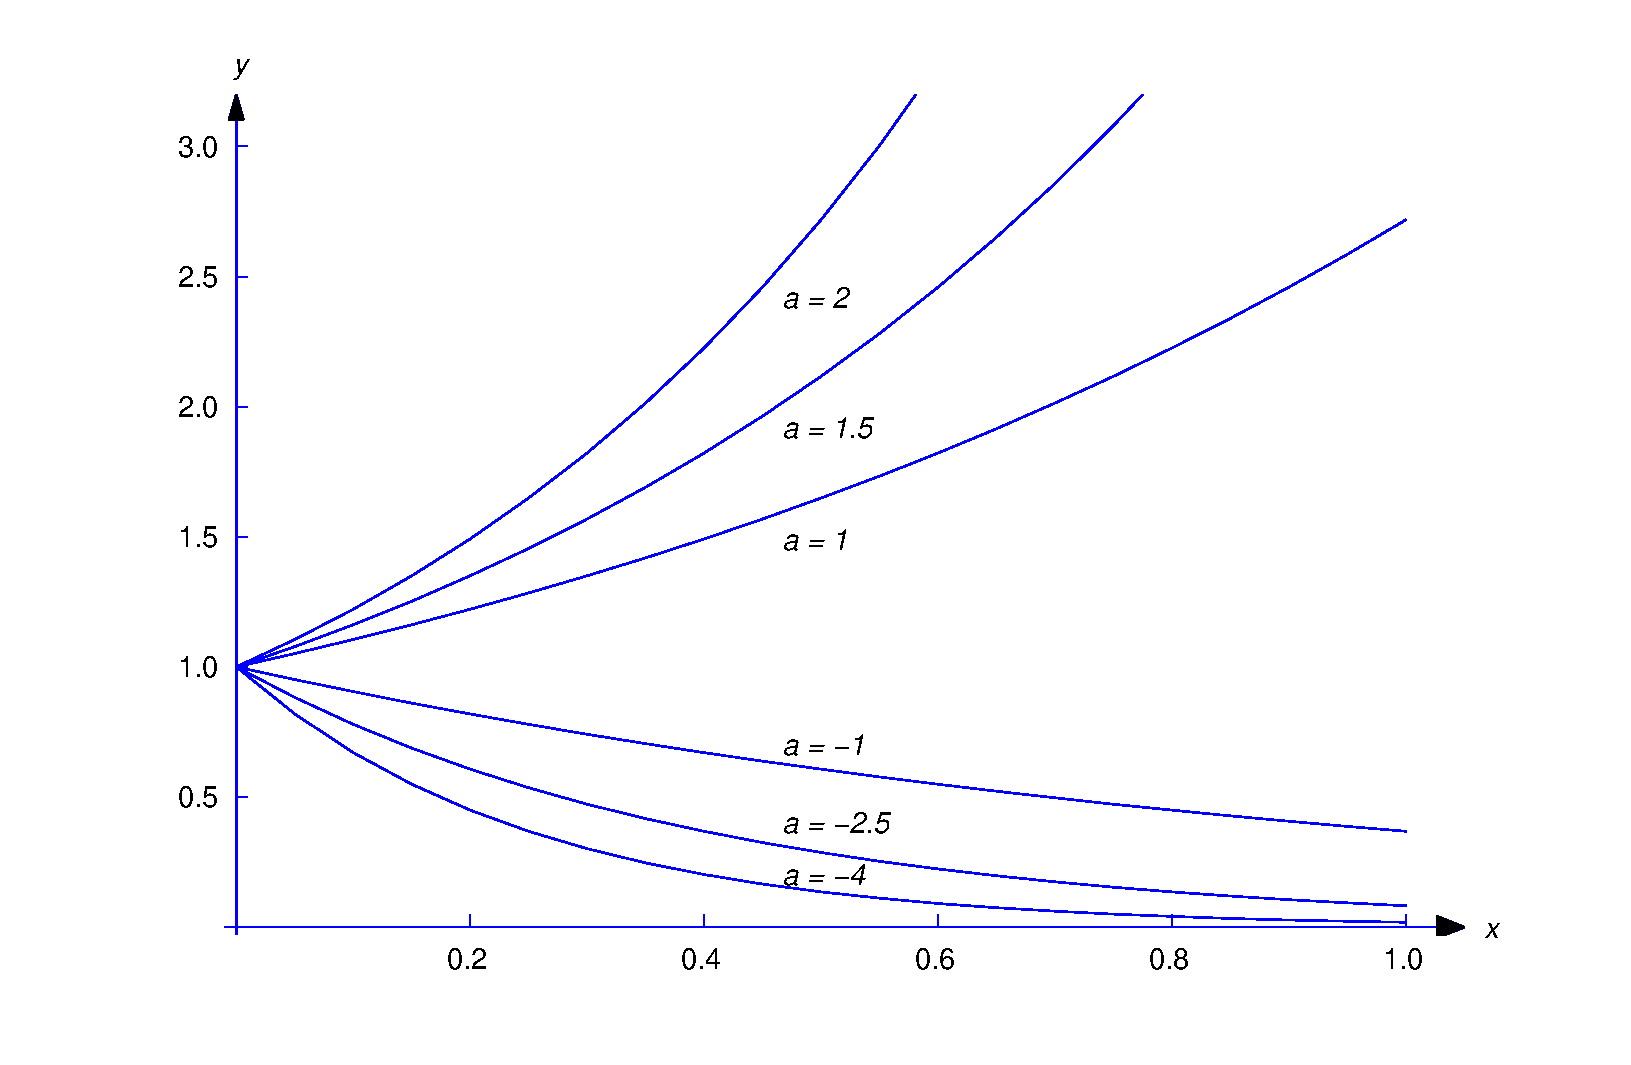
\includegraphics[bb=-78 148 689 643,width=5.67in,height=3.66in,keepaspectratio]{fig020101}
\color{blue}
  \caption{Solutions of $y'-ay=0$, $y(0)=1$}
  \label{figure:2.1.1}
\end{figure}


\begin{example} \label{example:2.1.4}\rm

\begin{alist}
\item % (a)
Find the general solution of
\begin{equation}
 xy'+y=0.\label{eq:2.1.8}
\end{equation}

\item % (b)
Solve the initial value problem
\begin{equation}
 xy'+y=0,\quad y(1)=3.\label{eq:2.1.9}
\end{equation}
\end{alist}
\end{example}


\solutionpart{a}
We rewrite \eqref{eq:2.1.8} as
\begin{equation}\label{eq:2.1.10}
y'+{1\over x}y=0,
\end{equation}
where $x$ is restricted to either $(-\infty,0)$ or $(0,\infty)$. If
$y$ is a nontrivial solution of \eqref{eq:2.1.10}, there must be some
open interval I on which $y$ has no zeros. We can rewrite
\eqref{eq:2.1.10} as
$$
{y'\over y}=-{1\over x}
$$
for $x$ in $I$. Integrating shows that
$$
\ln|y|=-\ln|x|+k,\mbox{\quad so\quad}|y|={e^k\over|x|}.
$$
Since a function that satisfies the last equation can't change sign on
either $(-\infty,0)$ or $(0,\infty)$, we can rewrite this result more
simply as
\begin{equation}\label{eq:2.1.11}
y={c\over x}
\end{equation}
where
$$
c=\left\{\begin{array}{cl}\phantom{-}e^k&\mbox{if } y>0,
\\ -e^k&\mbox{if } y<0.\end{array}\right.
$$
We've now shown that every solution of \eqref{eq:2.1.10} is given by
\eqref{eq:2.1.11} for some choice of $c$. (Even though we assumed that $y$
was nontrivial to derive \eqref{eq:2.1.11}, we can get the trivial
solution by setting $c=0$ in \eqref{eq:2.1.11}.) Conversely, any function
of the form \eqref{eq:2.1.11} is a solution of \eqref{eq:2.1.10}, since
differentiating \eqref{eq:2.1.11} yields
$$
y'=-{c\over x^2},
$$
and substituting this and \eqref{eq:2.1.11} into  \eqref{eq:2.1.10} yields
\begin{eqnarray*}
y'+{1\over x}y&=&-{c\over x^2}+{1\over x}{c\over x}\\[2\jot]
&=&-{c\over x^2}+{c\over x^2}=0.
\end{eqnarray*}

Figure~\ref{figure:2.1.2} shows the graphs of some solutions corresponding
to various values of $c$


\solutionpart{b} Imposing the initial condition $y(1)=3$ in
\eqref{eq:2.1.11} yields $c=3$. Therefore the solution of \eqref{eq:2.1.9} is
$$
y={3\over x}.
$$
The interval of validity of this solution is  $(0,\infty)$.


   \begin{figure}[tbp]
  \centering
  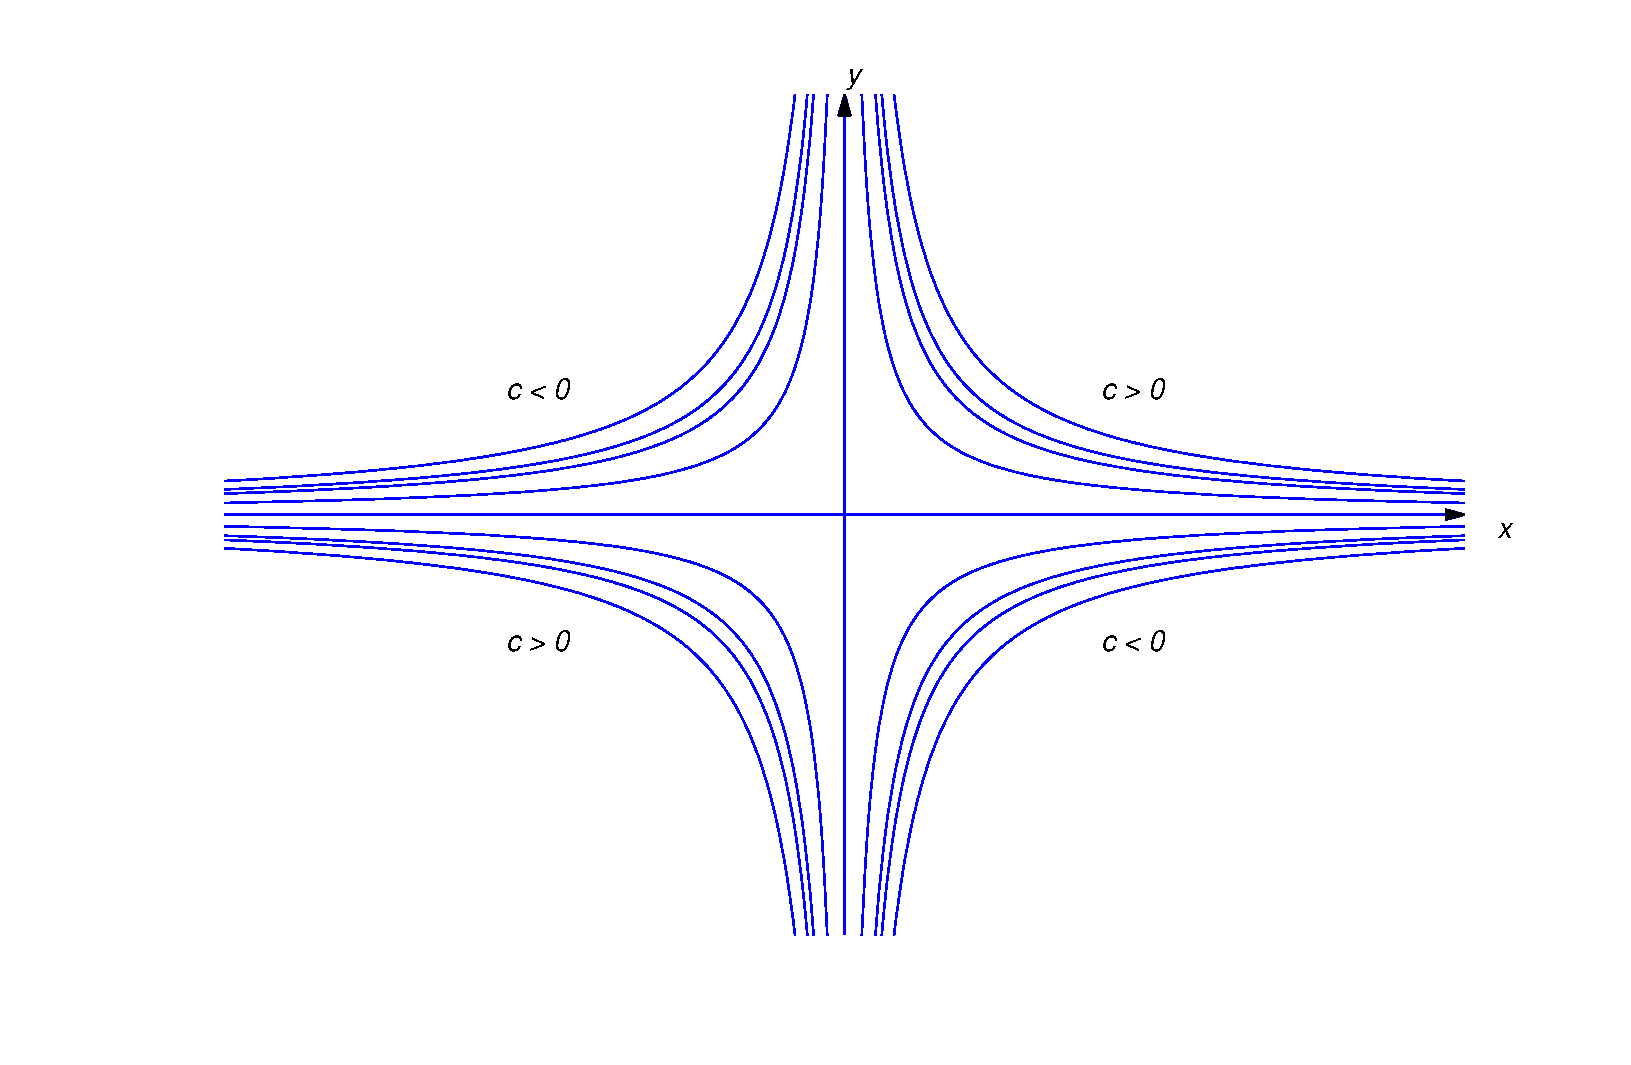
\includegraphics[bb=-78 148 689 643,width=5.67in,height=3.66in,keepaspectratio]{fig020102}
\color{blue}
  \caption{Solutions of $xy'+y=0$ on $(0,\infty)$ and
$(-\infty,0)$}
  \label{figure:2.1.2}
\end{figure}



The results in Examples~\ref{example:2.1.3}\part{a}  and
\ref{example:2.1.4}\part{b}
are special cases of the next theorem.

\begin{theorem}\color{blue}\label{thmtype:2.1.1}
If $p$ is continuous on $(a,b),$ then the general solution
of the homogeneous equation
\begin{equation}\label{eq:2.1.12}
y'+p(x)y=0
\end{equation}
on $(a,b)$ is
$$
y=ce^{-P(x)},
$$
where
\begin{equation}\label{eq:2.1.13}
P(x)=\int p(x)\,dx
\end{equation}
is any antiderivative of $p$ on $(a,b);$ that is$,$
\begin{equation}\label{eq:2.1.14}
P'(x)=p(x),\quad a<x<b.
\end{equation}
\end{theorem}

\proof
If $y=ce^{-P(x)}$,  differentiating $y$ and using \eqref{eq:2.1.14}
shows that
$$
y'=-P'(x)ce^{-P(x)}=-p(x)ce^{-P(x)}=-p(x)y,
$$
so $y'+p(x)y=0$; that is, $y$ is a solution of \eqref{eq:2.1.12}, for
any choice of $c$.

Now we'll show that any solution of \eqref{eq:2.1.12} can be written as
$y=ce^{-P(x)}$ for some constant $c$. The trivial solution can be
written this way, with $c=0$. Now suppose   $y$ is a nontrivial
solution. Then there's an open subinterval $I$ of $(a,b)$ on which
$y$ has no zeros. We can rewrite \eqref{eq:2.1.12} as
\begin{equation}\label{eq:2.1.15}
{y'\over y}=-p(x)
\end{equation}
for $x$ in $I$. Integrating \eqref{eq:2.1.15} and recalling \eqref{eq:2.1.13}
yields
$$
\ln|y|=-P(x) + k,
$$
where $k$ is a constant. This implies that
$$
|y|=e^ke^{-P(x)}.
$$
Since $P$ is defined for all $x$ in $(a,b)$  and an exponential can
never equal zero,  we can take $I=(a,b)$, so $y$
has zeros on $(a,b)$
$(a,b)$, so we can rewrite the last equation as $y=ce^{-P(x)}$, where
$$
c=\left\{\begin{array}{cl}\phantom{-}e^k&\mbox{if } y>0\mbox{ on }
(a,b),\\ -e^k&\mbox{if } y<0\mbox{ on }(a,b).\end{array}\right.
$$

\color{blue}
\remark{Rewriting a first order differential equation so that one
side depends only on $y$ and $y'$ and the other depends only on $x$
is called {\color{blue}\it separation of variables\/}. We did this in
Examples~ \ref{example:2.1.3} and  \ref{example:2.1.4}, and in rewriting
\eqref{eq:2.1.12} as \eqref{eq:2.1.15}.We'llapply this method to nonlinear
equations in Section~2.2.}
\color{black}

\boxit{Linear Nonhomogeneous First Order Equations}


\noindent
We'll now solve the nonhomogeneous equation
\begin{equation}\label{eq:2.1.16}
y'+p(x)y=f(x).
\end{equation}
When considering this equation  we call
$$
y'+p(x)y=0
$$
the {\color{blue}\it complementary equation}.

We'll find solutions of \eqref{eq:2.1.16} in the form $y=uy_1$, where
$y_1$ is a nontrivial solution of the complementary equation and $u$
is to be determined. This method of using a solution of the
complementary equation to obtain solutions of a nonhomogeneous
equation is a special case of a method called {\color{blue}\it variation of
parameters\/}, which you'll encounter several times in this book.
(Obviously, $u$ can't be constant, since if it were, the left side
of \eqref{eq:2.1.16} would be zero. Recognizing this, the early users of
this method viewed $u$ as a ``parameter'' that varies; hence, the name
``variation of parameters.'')

If
$$
y=uy_1,\mbox{\quad then\quad} y'=u'y_1+uy_1'.
$$
Substituting these expressions for $y$ and $y'$ into \eqref{eq:2.1.16}
yields
$$
u'y_1+u(y_1'+p(x)y_1)=f(x),
$$
which reduces to
\begin{equation}\label{eq:2.1.17}
u'y_1=f(x),
\end{equation}
since $y_1$ is a solution of the complementary equation; that is,
$$
y_1'+p(x)y_1=0.
$$
In the proof of Theorem~\ref{thmtype:2.2.1} we saw that $y_1$
has no zeros on an interval where $p$ is continuous. Therefore
we can divide \eqref{eq:2.1.17} through by $y_1$ to obtain
$$
u'=f(x)/y_1(x).
$$
We can integrate this (introducing a constant of integration), and
multiply  the result by $y_1$ to get the general solution of
\eqref{eq:2.1.16}.
Before turning to the formal proof of this claim, let's consider
some examples.

\begin{example}\label{example:2.1.5}\rm
Find the general solution of
\begin{equation}\label{eq:2.1.18}
y'+2y=x^3e^{-2x}.
\end{equation}
\end{example}



By applying \part{a} of Example~ \ref{example:2.1.3} with $a=-2$, we see
that $y_1=e^{-2x}$ is a solution of the  complementary equation
$y'+2y=0$. Therefore we seek solutions of \eqref{eq:2.1.18} in the form
 $y=ue^{-2x}$,  so that
\begin{equation} \label{eq:2.1.19}
 y'=u'e^{-2x}-2ue^{-2x}\mbox{\quad  and \quad }
y'+2y=u'e^{-2x}-2ue^{-2x}+2ue^{-2x}=u'e^{-2x}.
\end{equation}
Therefore $y$ is a solution of \eqref{eq:2.1.18} if and only if
$$
u'e^{-2x}=x^3e^{-2x}\mbox{\quad or, equivalently,\quad} u'=x^3.
$$
Therefore
$$
u={x^4\over4}+c,
$$
and
$$
y=ue^{-2x}=e^{-2x}\left({x^4\over4}+c\right)
$$
is the general  solution of \eqref{eq:2.1.18}.

Figure~\ref{figure:2.1.3} shows a direction field and some integral curves
for \eqref{eq:2.1.18}.

\begin{figure}[tbp]
  \centering
  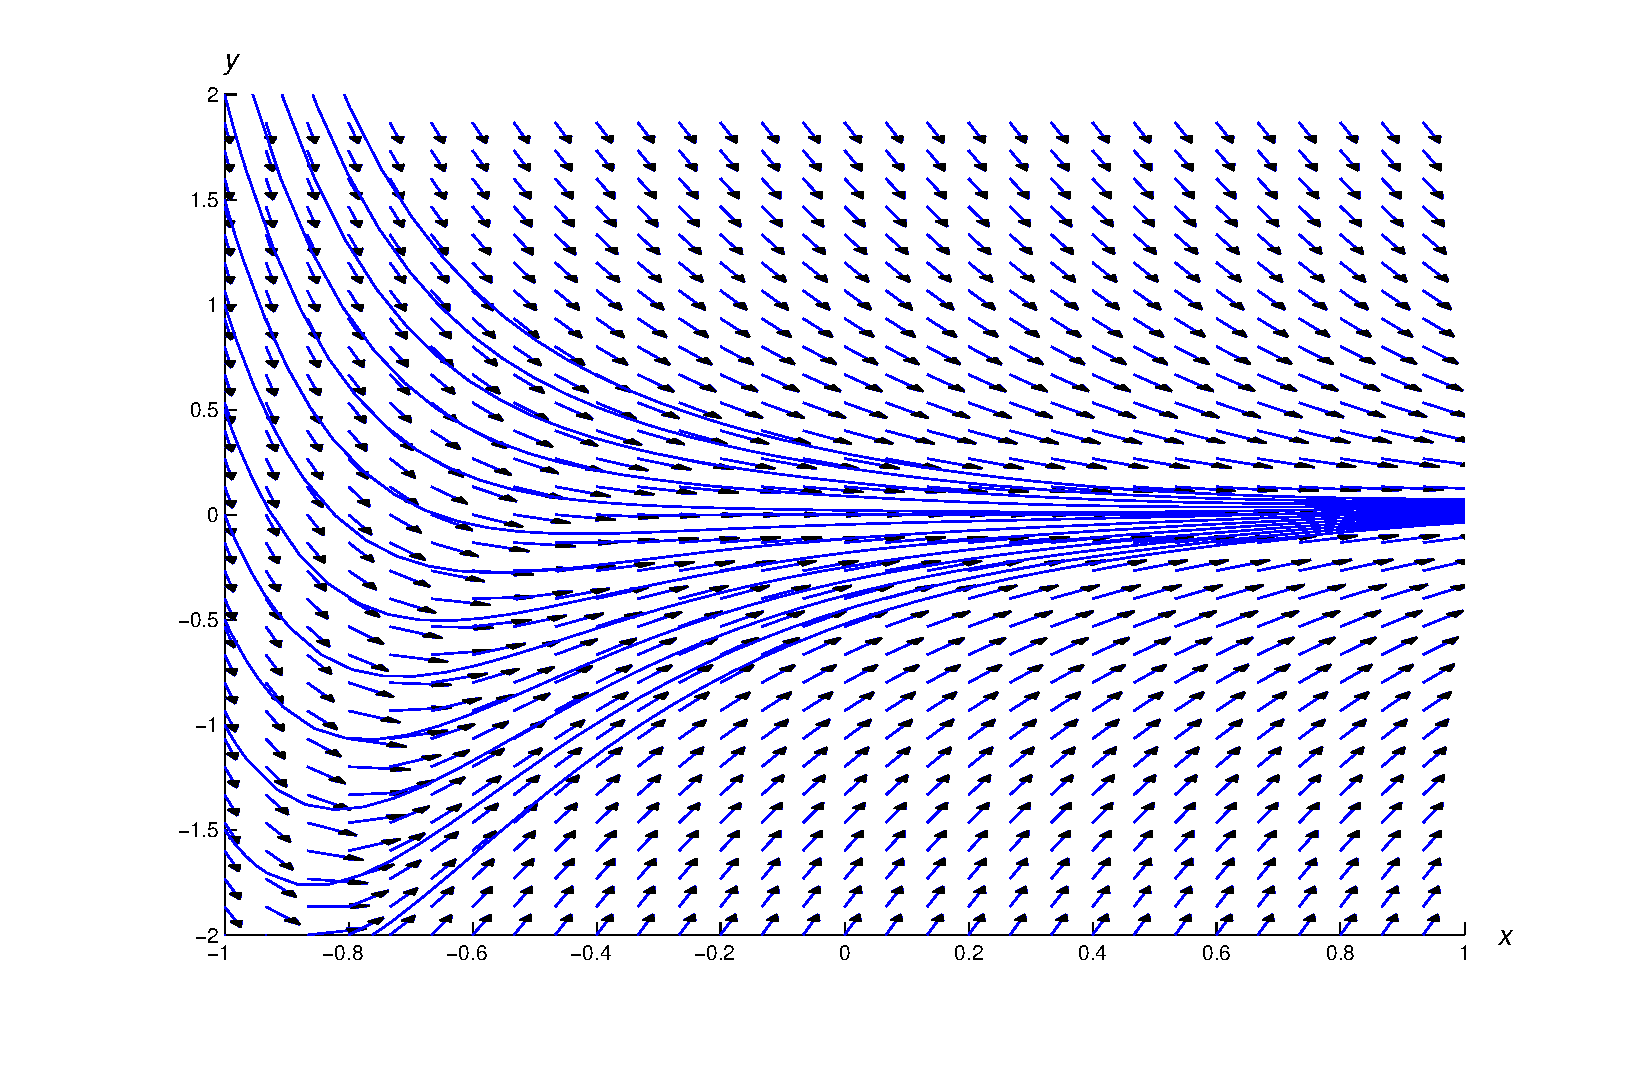
\includegraphics[bb=-78 148 689 643,width=5.67in,height=3.66in,keepaspectratio]{fig020103}
\color{blue}
  \caption{A direction field and integral curves for $y'+2y=x^{2}e^{-2x}$}
  \label{figure:2.1.3}
\end{figure}





\begin{example}\label{example:2.1.6}\rm\mbox{}%\newline
\begin{alist}
\item %(a)
Find the general solution
\begin{equation}\label{eq:2.1.20}
y'+(\cot x)y=x\csc x.
\end{equation}
\item %(b)
Solve the initial value problem
\begin{equation}\label{eq:2.1.21}
y'+(\cot x)y=x\csc x,\quad y(\pi/2)=1.
\end{equation}
\end{alist}
\end{example}



\solutionpart{a} Here $p(x)=\cot x$ and $f(x)= x\csc x$ are both
continuous except at the points $x=r\pi$, where $r$ is an integer.
Therefore we seek solutions of \eqref{eq:2.1.20} on the intervals
$\left(r\pi, (r+1)\pi \right)$.
We need a nontrival solution $y_1$ of
the complementary equation;   thus, $y_1$ must satisfy
 $y_1'+(\cot x)y_1=0$, which we rewrite as
\begin{equation}\label{eq:2.1.22}
{y_1'\over y_1}=-\cot x=-{\cos x\over\sin x}.
\end{equation}
Integrating this yields
$$
\ln|y_1|=-\ln|\sin x|,
$$
where we take the constant of integration to be zero since we need
only {\color{blue}\it one\/} function that satisfies \eqref{eq:2.1.22}. Clearly
$y_1=1/\sin x$ is a suitable choice. Therefore we seek solutions of
\eqref{eq:2.1.20} in the form
$$
y={u\over\sin x},
$$
so that
\begin{equation} \label{eq:2.1.23}
 y'={u'\over\sin x}-{u\cos x\over\sin^2x}
\end{equation}
and
\begin{equation} \label{eq:2.1.24}
\begin{array}{rcl}
y'+(\cot x)y&=&
\dst{u'\over\sin x}-\dst{u\cos x\over\sin^2x}+\dst{u\cot x\over\sin
x}\\[2\jot]
&=&\dst{u'\over\sin x}-\dst{u\cos x\over\sin^2x}+\dst{u\cos
x\over\sin^2 x}\\[2\jot]
&=&\dst{u'\over\sin x}.
\end{array}
\end{equation}
Therefore $y$ is a solution of \eqref{eq:2.1.20} if and only if
$$
u'/\sin x=x\csc x=x/\sin x\mbox{\quad or, equivalently, \quad} u'=x.
$$
Integrating this yields
\begin{equation}\label{eq:2.1.25}
u={x^2\over2}+c, \text{\quad and \quad }
y={u\over\sin x}= {x^2\over 2\sin x}+ {c\over\sin x}.
\end{equation}
is the general solution of \eqref{eq:2.1.20} on every interval
$\left(r\pi,(r+1)\pi\right)$ ($r=$integer).


\solutionpart{b}
Imposing the initial condition $y(\pi/2)=1$ in \eqref{eq:2.1.25} yields
$$
1={\pi^2\over 8}+c\mbox{\quad or\quad} c=1-{\pi^2\over 8}.
$$
 Thus,
$$
y={x^2\over 2\sin x}+{(1-\pi^2/8)\over\sin x}
$$
is a solution of \eqref{eq:2.1.21}.
The interval of validity of this solution is $(0,\pi)$;
Figure~\ref{figure:2.1.4} shows its graph.


   \begin{figure}[H]
  \centering
\scalebox{.8} { 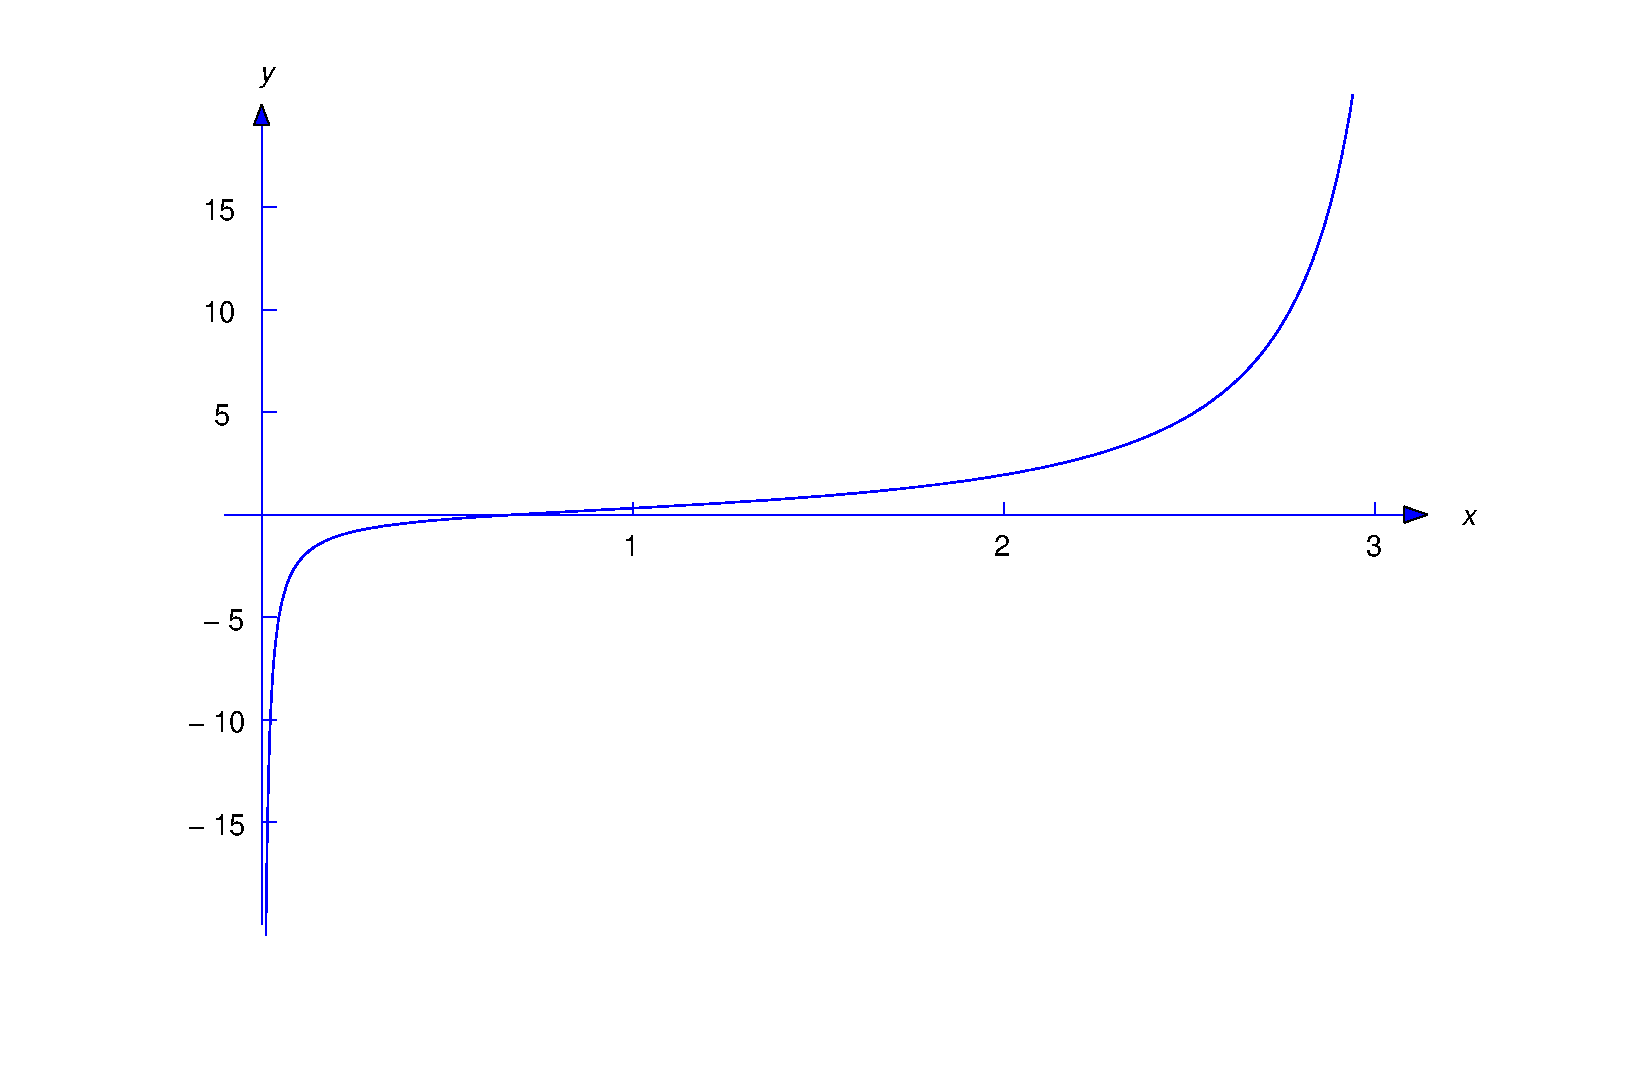
\includegraphics[bb=-78 148 689
643,width=5.67in,height=3.66in,keepaspectratio]{fig020104}}
\color{blue}
\caption{Solution of
$y'+(\cot x)y=x\csc x, y(\pi/2)=1$}
  \label{figure:2.1.4}
\end{figure}


\color{blue}
\remark{It wasn't necessary to do the computations
\eqref{eq:2.1.23} and \eqref{eq:2.1.24} in
Example~\ref{example:2.1.6}, since we showed in the discussion preceding
Example~\ref{example:2.1.5} that if $y=uy_1$ where $y_1'+p(x)y_1=0$,
then
$y'+p(x)y=u'y_1$. We did these computations so you would see this
happen in this specific example. We recommend that you include these
``unnecesary'' computations in doing exercises, until you're confident
that you really understand the method. After that, omit them.}
\color{black}

\medskip


We summarize the method  of variation of parameters for
solving

\begin{equation} \label{eq:2.1.26}
y'+p(x)y=f(x)
\end{equation}
as follows:

\medskip
\color{blue}
\begin{alist}
\item % (a)
Find a function $y_1$  such that
$$
{y_1'\over y_1}=-p(x).
$$
For convenience, take the constant of integration to be zero.
\item % (b)
Write
\begin{equation} \label{eq:2.1.27}
y=uy_1
\end{equation}
to remind yourself of what you're doing.
\item % (c)
Write $u'y_1=f$ and solve for $u'$;   thus, $u'=f/y_1$.
\item % (d
Integrate $u'$ to obtain $u$, with an arbitrary constant of
integration.
\item % (e)
Substitute $u$ into \eqref{eq:2.1.27}  to obtain $y$.
\end{alist}
\color{black}

\medskip
To solve an equation written as
$$
P_0(x)y'+P_1(x)y=F(x),
$$
we recommend that you divide through by $P_0(x)$ to obtain an equation
of the form  \eqref{eq:2.1.26}
and then follow this   procedure.

\boxit{Solutions in Integral Form}


\noindent
Sometimes the integrals that arise in solving a linear first order
equation can't be evaluated in terms of elementary functions. In this
case the solution must be left in terms of an integral.

\begin{example}\label{example:2.1.7}\rm  \mbox{}\newline
\begin{alist}
\item % (a)
Find the general solution of
$$
y'-2xy=1.
$$
\item % (b)
Solve the initial value problem
\begin{equation}\label{eq:2.1.28}
y'-2xy=1,\quad y(0)=y_0.
\end{equation}
\end{alist}
\end{example}

\solutionpart{a}
To apply variation of parameters, we need a nontrivial solution $y_1$
of  the complementary equation;   thus,
$y_1'-2xy_1=0$, which we rewrite as
$$
{y_1'\over y_1}=2x.
$$
Integrating this and taking the constant of integration to be
zero yields
$$
\ln|y_1|=x^2,\mbox{\quad so \quad}|y_1|=e^{x^2}.
$$
We choose $y_1=e^{x^2}$ and seek solutions of
 \eqref{eq:2.1.28} in the form $y=ue^{x^2}$, where
$$
u'e^{x^2}=1,\mbox{\quad so \quad} u'=e^{-x^2}.
$$
Therefore
$$
u=c+\int e^{-x^2}dx,
$$
 but we can't simplify the integral on the right because
there's  no elementary function with  derivative equal to $e^{-x^2}$.
Therefore the best available form for the  general solution of
\eqref{eq:2.1.28} is
\begin{equation}\label{eq:2.1.29} y=ue^{x^2}= e^{x^2}\left(c+\int
e^{-x^2}dx\right). \end{equation}

\solutionpart{b}
  Since the initial condition in \eqref{eq:2.1.28}
is imposed at $x_0=0$, it is convenient to rewrite \eqref{eq:2.1.29} as
$$
y=e^{x^2}\left(c+\int^x_0 e^{-t^2} dt\right),\mbox{\quad since
\quad} \int_0^0e^{-t^2}\,dt=0.
$$
 Setting $x=0$ and $y=y_0$ here shows that
$c=y_0$.  Therefore the solution of the initial value problem is
\begin{equation}\label{eq:2.1.30}
y=e^{x^2}\left(y_0 +\int^x_0 e^{-t^2}dt\right).
\end{equation}
For a given value of $y_0$ and each fixed $x$, the integral on the
right can be evaluated by numerical methods. An alternate procedure is
to apply the numerical integration procedures discussed in
Chapter~3 directly to the initial value problem
\eqref{eq:2.1.28}.
Figure~\ref{figure:2.1.5} shows graphs of
 of \eqref{eq:2.1.30} for several values of $y_0$.



\begin{figure}[H]
  \centering
\scalebox{.9}{
  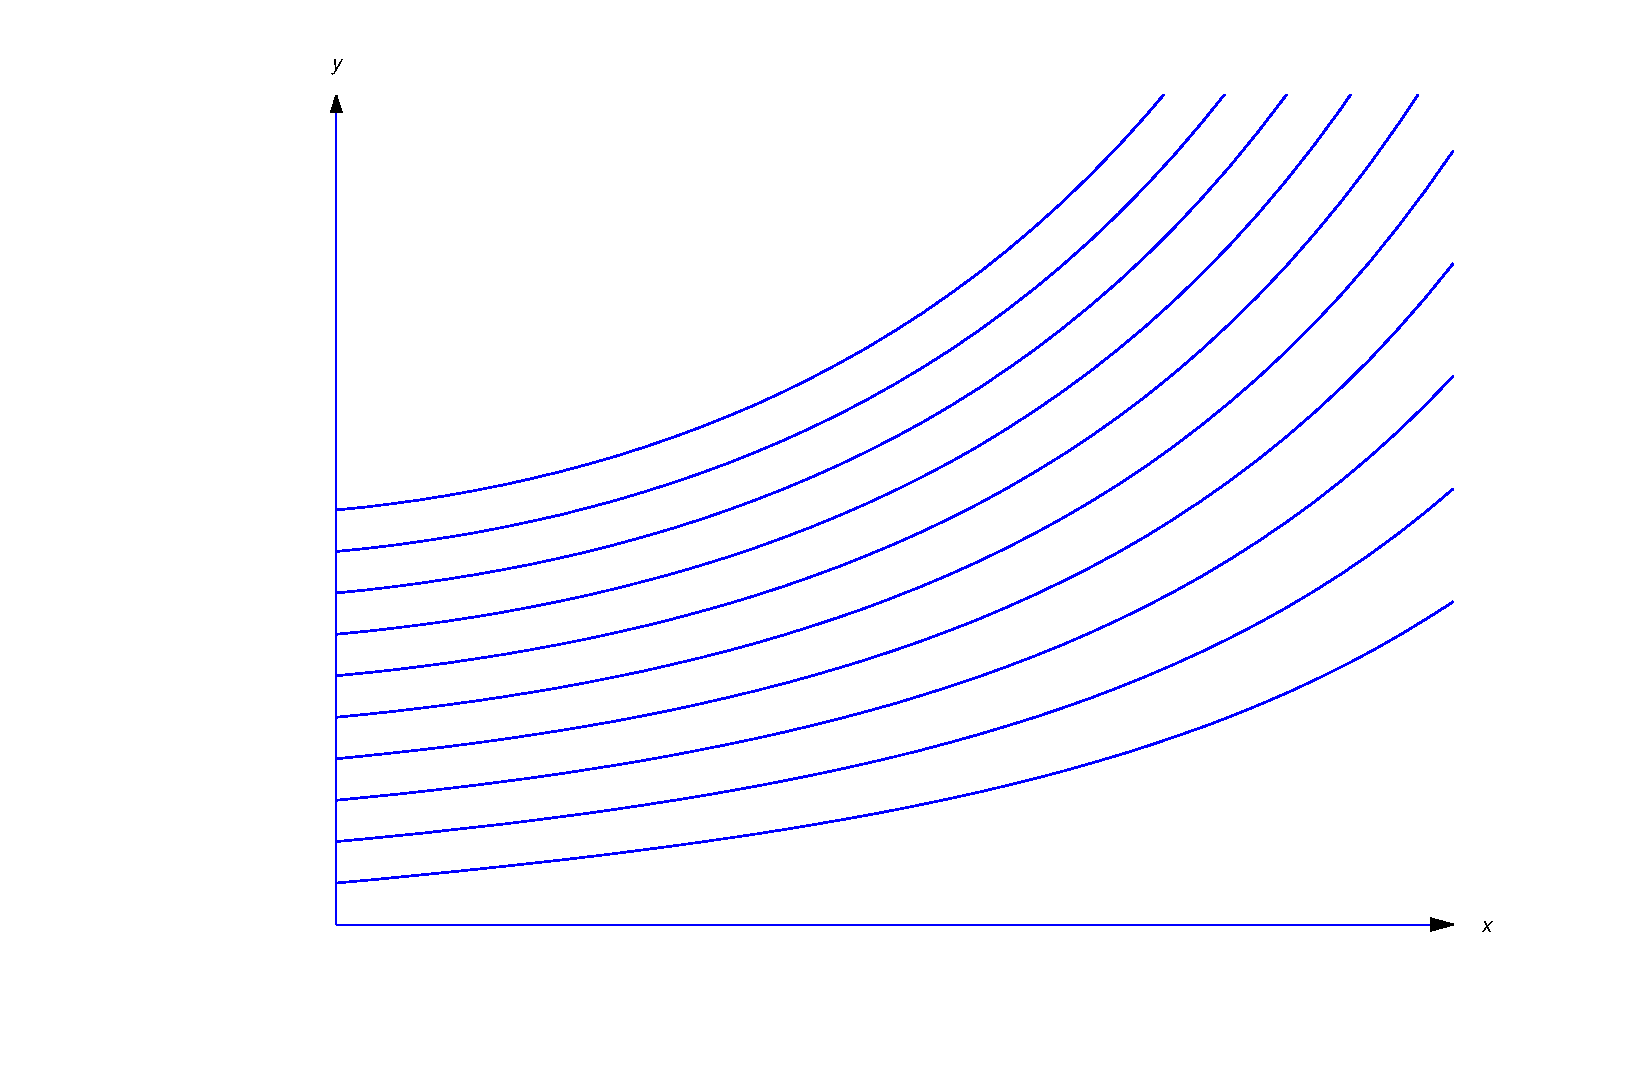
\includegraphics[bb=-78 148 689 643,width=5.67in,height=3.66in,keepaspectratio]{fig020105} }
\color{blue}
  \caption{Solutions of $y'-2xy=1$, $y(0)=y_{0}$}
  \label{figure:2.1.5}
\end{figure}

\boxit{An Existence and Uniqueness Theorem}

\noindent
The method of variation of parameters leads to this theorem.

\begin{theorem}\color{blue}\label{thmtype:2.1.2}
 Suppose  $p$ and
$f$ are continuous on an open interval $(a,b),$  and let $y_1$ be any
nontrivial solution of the complementary equation
$$
y'+p(x)y=0
$$
on $(a,b)$.
Then$:$
\begin{alist}
\item % (a)
The general solution of the nonhomogeneous equation
\begin{equation}\label{eq:2.1.31}
y'+p(x)y=f(x)
\end{equation}
 on  $(a,b)$ is
\begin{equation}\label{eq:2.1.32}
y=y_1(x)\left(c +\int f(x)/y_1(x)\,dx\right).
\end{equation}
\item % (b)
If $x_0$ is an arbitrary point in $(a,b)$ and $y_0$ is an arbitrary
real number$,$ then the initial value problem
$$
y'+p(x)y=f(x),\quad y(x_0)=y_0
$$
 has the unique solution
$$
y=y_1(x)\left({y_0\over y_1(x_0)} +\int^x_{x_0} {f(t)\over
y_1(t)}\, dt\right)
$$
on $(a,b).$
\end{alist}
\end{theorem}

\proof \part{a} To show that \eqref{eq:2.1.32} is the general solution of
\eqref{eq:2.1.31} on $(a,b)$, we must prove that:

\begin{rmlist}
\item % (i)
If $c$ is any constant,   the function $y$ in
\eqref{eq:2.1.32} is a solution of \eqref{eq:2.1.31} on  $(a,b)$.
\item % (ii)
  If $y$ is a solution of \eqref{eq:2.1.31} on  $(a,b)$ then $y$
is of the form  \eqref{eq:2.1.32} for some constant~$c$.
\end{rmlist}

To prove \part{i}, we first observe that any function of the form
\eqref{eq:2.1.32} is defined on $(a,b)$, since $p$ and $f$ are continuous
on $(a,b)$. Differentiating \eqref{eq:2.1.32} yields
$$
y'=y_1'(x)\left(c +\int f(x)/y_1(x)\,
dx\right)+f(x).
$$
Since $y_1'=-p(x)y_1$, this and \eqref{eq:2.1.32} imply that
\begin{eqnarray*}
y'&=&-p(x)y_1(x)\left(c +\int f(x)/y_1(x)\, dx\right)+f(x)\\
&=&-p(x)y(x)+f(x),
\end{eqnarray*}
which implies that $y$ is a solution of \eqref{eq:2.1.31}.

To prove \part{ii}, suppose   $y$ is a solution of \eqref{eq:2.1.31}
on $(a,b)$. From the proof of Theorem~\ref{thmtype:2.1.1}, we know that
$y_1$ has no zeros on $(a,b)$, so the function $u=y/y_1$ is defined
on $(a,b)$. Moreover, since
$$
y'=-py+f\mbox{\quad and\quad}y_1'=-py_1,
$$
\begin{eqnarray*}
u'&=&{y_1y'-y_1'y\over y_1^2}\\[2\jot]
&=&{y_1(-py+f)-(-py_1)y\over y_1^2}={f\over y_1}.
\end{eqnarray*}
Integrating $u'=f/y_1$ yields
$$
u=\left(c +\int f(x)/y_1(x)\, dx\right),
$$
which implies \eqref{eq:2.1.32}, since $y=uy_1$.

\part{b} We've proved \part{a}, where $\int f(x)/y_1(x)\,dx$ in
\eqref{eq:2.1.32}
is an arbitrary antiderivative of $f/y_1$. Now it's convenient to
choose the antiderivative that equals zero when $x=x_0$, and write the
general solution of \eqref{eq:2.1.31} as
$$
y=y_1(x)\left(c +\int^x_{x_0} {f(t)\over
y_1(t)}\, dt\right).
$$
Since
$$
y(x_0)= y_1(x_0)\left(c +\int^{x_0}_{x_0} {f(t)\over
y_1(t)}\, dt\right)=cy_1(x_0),
$$
we see that
 $y(x_0)=y_0$ if and only if $c=y_0/y_1(x_0)$.

\exercises
In Exercises~\ref{exer:2.1.1}--\ref{exer:2.1.5} find
the general solution.


\begin{exerciselist}


\begin{tabular}[t]{@{}p{168pt}@{}p{168pt}}
\item\label{exer:2.1.1} $y'+ay=0$ ($a$=constant)
&\item\label{exer:2.1.2}\vspace*{10pt} $y'+3x^2y=0$
\end{tabular}

\begin{tabular}[t]{@{}p{168pt}@{}p{168pt}}
\item\label{exer:2.1.3} $xy'+(\ln x)y=0$
&\item\label{exer:2.1.4} $xy'+3y=0$
\end{tabular}

\begin{tabular}[t]{@{}p{168pt}@{}p{168pt}}
\item\label{exer:2.1.5} $x^2y'+y=0$ &
\end{tabular}

\exercisetext{In Exercises~\ref{exer:2.1.6}--\ref{exer:2.1.11} solve
the initial value problem.}

\item\label{exer:2.1.6}
$\dst{y'+\left({1+x\over x}\right)y=0,\quad y(1)=1}$

\item\label{exer:2.1.7}
$\dst{xy'+\left(1+{1\over\ln x}\right)y=0,\quad y(e)=1}$

\item\label{exer:2.1.8}
$\dst{xy'+(1+ x\cot x)y=0,\quad y\left({\pi\over 2}
\right)=2}$

\item\label{exer:2.1.9}
$\dst{y'-\left({2x\over 1+x^2}\right)y=0,\quad y(0)=2}$

\item\label{exer:2.1.10}
$\dst{y'+{k\over x}y=0,\quad y(1)=3 \quad\mbox{($k$=
constant)}}$


\item\label{exer:2.1.11}
$\dst y'+(\tan kx)y=0,\quad y(0)=2 \quad\mbox{($k=$ constant)}$

\exercisetext{In Exercises~\ref{exer:2.1.12} --\ref{exer:2.1.15} find
the general solution. Also, plot a direction field and some integral
curves on the rectangular region $\{-2\le x\le2,\ -2\le y\le2$\}.}

\begin{tabular}{@{}p{168pt}@{}p{168pt}}
\item\label{exer:2.1.12} \CGex $y'+3y=1$
&\item\label{exer:2.1.13}\vspace*{6pt} \CGex $\dst{y'+\left({1\over x}-
1\right)y=-{2\over x}}$
\end{tabular}


\begin{tabular}{@{}p{168pt}@{}p{168pt}}
\item\label{exer:2.1.14} \CGex
$y'+2xy=xe^{-x^2}$ &
\item\label{exer:2.1.15} \CGex
$\dst{y'+{2x\over1+x^2}y={e^{-x}\over1+x^2}}$
\end{tabular}

\exercisetext{In Exercises~\ref{exer:2.1.16} --\ref{exer:2.1.24} find
the general solution.}


\begin{tabular}[t]{@{}p{168pt}@{}p{168pt}}
\item\label{exer:2.1.16} $\dst{y'+{1\over x}y={7\over
x^2}+3}$
&\item\label{exer:2.1.17}\vspace*{8pt} $\dst{y'+{4\over x-1}y
= {1\over (x-1)^5}+{\sin x\over (x-1)^4}}$
\end{tabular}

\begin{tabular}[t]{@{}p{168pt}@{}p{168pt}}
\item\label{exer:2.1.18} $xy'+(1+2x^2)y=x^3e^{-x^2}$
&\item\label{exer:2.1.19}\vspace*{-8pt} $\dst{xy'+2y={2\over
x^2}+1}$\end{tabular}

\begin{tabular}[t]{@{}p{168pt}@{}p{168pt}}
\item\label{exer:2.1.20} $y'+(\tan x)y=\cos x$
&\item\label{exer:2.1.21}\vspace*{-5pt} $\dst{(1+x)y'+2y={\sin x
\over 1 + x}}$
\end{tabular}

\item\label{exer:2.1.22}
$(x-2)(x-1)y'-(4x-3)y=(x-2)^3$

\begin{tabular}[t]{@{}p{168pt}@{}p{168pt}}
\item\label{exer:2.1.23}
$y'+(2\sin x\cos x) y=e^{-\sin^2x}$&
\item\label{exer:2.1.24}
$x^2y'+3xy=e^x$
\end{tabular}

\exercisetext{In Exercises~\ref{exer:2.1.25}--\ref{exer:2.1.29} solve the
initial value problem and sketch the graph of the solution.}

\item\label{exer:2.1.25} \CGex $y'+7y=e^{3x},\quad y(0)=0$

\item\label{exer:2.1.26} \CGex
$\dst{(1+x^2)y'+4xy={2\over 1+x^2},\quad y(0)=1}$

\item\label{exer:2.1.27} \CGex
$\dst{xy'+3y={2\over x(1+x^2)},\quad y(-1)=0}$


\item\label{exer:2.1.28} \CGex
$\dst{y'+ (\cot x)y=\cos x,\quad
y\left({\pi\over 2}\right)=1}$

\item\label{exer:2.1.29} \CGex
$\dst{y'+{1\over x}y={2\over x^2}+1,\quad y(-1)=0}$


\exercisetext{In Exercises~\ref{exer:2.1.30}--\ref{exer:2.1.37} solve
the initial value
problem.}

\item\label{exer:2.1.30}
$\dst{(x-1)y'+3y={1\over (x-1)^3} +
{\sin x\over (x-1)^2},\quad y(0)=1}$

\item\label{exer:2.1.31}
$xy'+2y=8x^2,\quad y(1)=3$

\item\label{exer:2.1.32}
$xy'-2y=-x^2,\quad y(1)=1$

\item\label{exer:2.1.33}
$y'+2xy=x,\quad y(0)=3$

\item\label{exer:2.1.34}
$\dst{(x-1)y'+3y={1+(x-1)\sec^2x\over (x-1)^3},\quad y(0)=-1}$

\item\label{exer:2.1.35}
$\dst{(x+2)y'+4y={1+2x^2\over x(x+2)^3},\quad y(-1)=2}$

\item\label{exer:2.1.36}
$(x^2-1)y'-2xy=x(x^2-1),\quad y(0)=4$

\item\label{exer:2.1.37}
$(x^2-5)y'-2xy=-2x(x^2-5),\quad y(2)=7$

\exercisetext{In Exercises~\ref{exer:2.1.38}--\ref{exer:2.1.42} solve
the initial value problem and leave the answer in a form involving a
definite integral. $($You can solve these problems numerically by
methods discussed in Chapter~3.$)$}

\item\label{exer:2.1.38}
$y'+2xy=x^2,\quad y(0)=3$

\item\label{exer:2.1.39}
$\dst{y'+{1\over x}y={\sin x\over x^2},\quad y(1)=2}$

\item\label{exer:2.1.40}
$\dst{y'+y={e^{-x}\tan x\over x},\quad y(1)=0}$

\item\label{exer:2.1.41}
$\dst{y'+{2x\over 1+x^2}y={e^x\over (1+x^2)^2}, \quad y(0)=1}$

\item\label{exer:2.1.42}
$xy'+(x+1)y=e^{x^2},\quad y(1)=2$

\item\label{exer:2.1.43}

Experiments indicate that glucose is absorbed by the body at a rate
proportional to the amount of glucose present in the bloodstream. Let
$\lambda$ denote the (positive) constant of proportionality. Now
suppose   glucose is injected into a patient's bloodstream at a
constant rate of $r$ units per unit of time. Let $G=G(t)$ be the
number of units in the patient's bloodstream at time $t>0$. Then
$$
G'=-\lambda G+r,
$$
where the first term on the right is due to the absorption of the
glucose by the patient's body and the second term is due to the
injection. Determine $G$ for $t>0$, given that $G(0)=G_0$. Also,
find $\lim_{t\to\infty}G(t)$.


\item\label{exer:2.1.44}
\begin{alist}
\item % (a)
\Lex Plot a direction field and some integral curves for
$$
xy'-2y=-1
\eqno{\rm (A)}
$$
on the rectangular region  $\{-1\le x\le 1, -.5\le y\le 1.5\}$.
What do all the integral curves have in common?
\item %(b)
Show that the general solution of (A)
on $(-\infty,0)$ and $(0,\infty)$ is
$$
y={1\over2}+cx^2.
$$
\item % (c)
Show that $y$ is a solution of (A) on
$(-\infty,\infty)$ if and only if
$$
y=\left\{\begin{array}{ll}\dst{{1\over2}+c_1x^2}, &x
\ge 0,\\[2\jot]
\dst{{1\over2}+c_2x^2}, &x < 0,\end{array}\right.
$$
 where $c_1$ and $c_2$ are arbitrary constants.
\item % (c)
Conclude from \part{c} that all solutions of (A) on
$(-\infty,\infty)$ are solutions of the initial value problem
$$
xy'-2y=-1,\quad y(0)={1\over2}.
$$
\item %(d)
Use \part{b} to show that if  $x_0\ne0$ and $y_0$  is arbitrary, then
  the  initial value problem
$$
xy'-2y=-1,\quad y(x_0)=y_0
$$
has infinitely many solutions on ($-\infty,\infty$). Explain why this
does'nt contradict  Theorem~\ref{thmtype:2.1.1}\part{b}.
\end{alist}


\item\label{exer:2.1.45}
Suppose $f$ is continuous on an open interval $(a,b)$
and $\alpha$ is a constant.
\begin{alist}
\item %(a)
Derive a formula for the solution of the initial value
problem
\renewcommand{\theequation}{\Alph{equation}}
$$
y'+\alpha y=f(x),\quad y(x_0)=y_0,
\eqno{\rm (A)}
$$
where $x_0$ is in $(a,b)$ and $y_0$ is an arbitrary real number.

\item %(b)
Suppose $(a,b)=(a,\infty)$, $\alpha > 0$ and
$\displaystyle{\lim_{x\to\infty} f(x)=L}$. Show that if $y$ is the
solution of (A), then $\displaystyle{\lim_{x\to
\infty} y(x)=L/\alpha}$.
\end{alist}

\item\label{exer:2.1.46}
Assume that all functions in this exercise are defined on
a common interval $(a,b)$.
\begin{alist}
\item %(a)
Prove:  If $y_1$ and $y_2$ are solutions of
$$
y'+p(x)y=f_1(x)
$$
and
$$
y'+p(x)y=f_2(x)
$$
respectively, and $c_1$ and $c_2$ are constants, then
$y=c_1y_1+c_2y_2$ is a solution of
$$
y'+p(x)y=c_1f_1(x)+c_2f_2(x).
$$
(This is the\it principle of superposition.\rm)

\item %(b)
Use \part{a} to show that if $y_1$ and $y_2$ are solutions
of the nonhomogeneous equation
$$
y'+p(x)y=f(x),
\eqno{\rm (A)}
$$
then $y_1-y_2$ is a solution of the homogeneous equation
$$
y'+p(x)y=0.
\eqno{\rm (B)}
$$

\item %(c)
Use \part{a} to show that if $y_1$ is a solution of
(A) and $y_2$ is a solution of
(B), then $y_1+y_2$ is a solution of
(A).
\end{alist}

\item\label{exer:2.1.47}
Some nonlinear equations can be transformed into linear
equations by changing the dependent variable.  Show that if
$$
g'(y)y'+p(x)g(y)=f(x)
$$
where $y$ is a function of $x$ and $g$ is a function of $y$,
then the new dependent variable $z=g(y)$ satisfies the
linear equation
$$
z'+p(x)z=f(x).
$$

\item\label{exer:2.1.48}
Solve by the method discussed in Exercise~\ref{exer:2.1.47}.

\vspace*{6pt}
\begin{tabular}[t]{@{}p{168pt}@{}p{168pt}}
{\bf (a)} $(\sec^2y)y'- 3\tan y=-1$
& {\bf (b)} $\dst{e^{y^2}\left(2yy'+
{2\over x}\right) ={1\over x^2}}$
\end{tabular}

\begin{tabular}[t]{@{}p{168pt}@{}p{168pt}}
{\bf (c)} $\dst{{xy'\over y} + 2\ln y=4x^2}$
& {\bf (d)} $\dst{{y'\over (1+y)^2} -
{1\over x(1+y)}=-{3\over x^2}}$
\end{tabular}

\item\label{exer:2.1.49}
We've shown that if $p$ and $f$ are continuous on $(a,b)$
then every solution of
$$
y'+p(x)y=f(x)
\eqno{\rm(A)}
$$
on $(a,b)$ can be written as $y=uy_1$, where
$y_1$ is a nontrivial solution of the complementary equation for (A)
and $u'=f/y_1$. Now suppose   $f$, $f'$, \dots, $f^{(m)}$ and
$p$, $p'$, \dots, $p^{(m-1)}$ are continuous on $(a,b)$, where $m$
is a positive integer, and define
\begin{eqnarray*}
f_0&=&f,\\ f_j&=&f_{j-1}'+pf_{j-1},\quad 1\le j\le m.
\end{eqnarray*}
Show that
$$
u^{(j+1)}={f_j\over y_1},\quad 0\le j\le m.
$$

\end{exerciselist}

\newsection{2}{First Order Equations} {Separable Equations}
\currentpdfbookmark{Section 2.2 Separable Equations}{section:2.2}
\vskip14pt
\renewcommand{\thissection}{\sectiontitle{\, SEPARABLE  EQUATIONS}}
\thissection



\noindent
A first order differential equation  is  {\color{blue}\it
separable} if it can be written as
\begin{equation} \label{eq:2.2.1}
h(y)y'=g(x),
\end{equation}
where the left side is a product of $y'$ and a function of $y$ and
the right side is a function of $x$. Rewriting a separable
differential equation in this form is called {\color{blue}\it separation of
variables.\/} In Section~2.1 we used separation of variables
to solve homogeneous linear equations. In this section we'll apply
this method to nonlinear equations.

To see how to solve \eqref{eq:2.2.1}, let's first assume that $y$
is a solution.
Let  $G(x)$ and $H(y)$ be antiderivatives of $g(x)$
and $h(y)$; that is,
\begin{equation} \label{eq:2.2.2}
H'(y)=h(y)\mbox{\quad and \quad}G'(x)=g(x).
\end{equation}
Then, from the chain rule,
$$
{d\over dx}H(y(x))=H'(y(x))y'(x)=h(y)y'(x).
$$
Therefore \eqref{eq:2.2.1} is equivalent to
$$
{d\over dx}H(y(x))={d\over dx}G(x).
$$
Integrating both sides of this equation and combining the constants of
integration yields
\begin{equation} \label{eq:2.2.3}
H(y(x))=G(x)+c.
\end{equation}
Although we derived this equation on the assumption that $y$
is a solution of \eqref{eq:2.2.1}, we can now view it differently:
Any differentiable function $y$ that satisfies \eqref{eq:2.2.3}
for some constant $c$ is a solution of \eqref{eq:2.2.1}. To see this, we
differentiate both sides of \eqref{eq:2.2.3}, using the chain rule on the
left, to obtain
$$
H'(y(x))y'(x)=G'(x),
$$
which is equivalent to
$$
h(y(x))y'(x)=g(x)
$$
because of \eqref{eq:2.2.2}.

In conclusion, to solve \eqref{eq:2.2.1} it suffices to find
functions $G=G(x)$ and $H=H(y)$ that satisfy \eqref{eq:2.2.2}.
Then any differentiable function  $y=y(x)$  that satisfies
\eqref{eq:2.2.3} is a solution of \eqref{eq:2.2.1}.

\begin{example}\label{example:2.2.1}\rm
Solve the equation
$$
y'=x(1+y^2).
$$
\end{example}


\solution Separating variables
yields
$$
{y'\over 1+y^2}=x.
$$
Integrating yields
$$
\tan^{-1}y={x^2\over2}+c
$$
Therefore
$$
y=\tan\left({x^2\over2}+c\right).
$$

\begin{example}\label{example:2.2.2} \rm  \mbox{}\newline
\begin{alist}
\item %(a)
Solve the equation
\begin{equation} \label{eq:2.2.4}
y'=-{x\over y}.
\end{equation}

\item %(b)
Solve the initial value problem
\begin{equation} \label{eq:2.2.5}
y'=-{x\over y}, \quad y(1)=1.
\end{equation}

\item %(c)
Solve the initial value problem
\begin{equation} \label{eq:2.2.6}
y'=-{x\over y}, \quad y(1)=-2.
\end{equation}
\end{alist}
\end{example}

\solutionpart{a} Separating variables
in \eqref{eq:2.2.4}  yields
$$
yy'=-x.
$$
Integrating yields
$$
{y^2\over2}=-{x^2\over2}+c,\mbox{\quad or,\, equivalently, \quad}
x^2+y^2=2c.
$$
The last equation shows that $c$ must be positive if $y$ is to be a
solution of \eqref{eq:2.2.4} on an open interval. Therefore we let
$2c=a^2$ (with $a > 0$) and rewrite the last equation as
\begin{equation} \label{eq:2.2.7}
x^2+y^2=a^2.
\end{equation}
 This equation has two differentiable solutions for $y$ in terms of
$x$:
\begin{equation} \label{eq:2.2.8}
y=\phantom{-} \sqrt{a^2-x^2}, \quad -a < x < a,
\end{equation}
 and
\begin{equation} \label{eq:2.2.9}
y= - \sqrt{a^2-x^2}, \quad -a < x < a.
\end{equation}
The solution curves defined by \eqref{eq:2.2.8}  are semicircles
above the
$x$-axis and  those defined by \eqref{eq:2.2.9}  are semicircles below the
$x$-axis (Figure~\ref{figure:2.2.1}).





\solutionpart{b}  The solution of  \eqref{eq:2.2.5}
is positive when $x=1$; hence, it  is of the form \eqref{eq:2.2.8}.
 Substituting $x=1$ and $y=1$ into \eqref{eq:2.2.7} to satisfy the
initial condition yields $a^2=2$; hence, the solution of
\eqref{eq:2.2.5}
is
$$
y=\sqrt{2-x^2}, \quad - \sqrt{2}< x < \sqrt{2}.
$$

\solutionpart{c}  The solution of  \eqref{eq:2.2.6}
is negative when $x=1$ and   is therefore of the form \eqref{eq:2.2.9}.
 Substituting $x=1$ and $y=-2$ into \eqref{eq:2.2.7} to satisfy the
initial condition yields $a^2=5$. Hence, the solution of \eqref{eq:2.2.6}
is
$$
y=- \sqrt{5-x^2}, \quad -\sqrt{5} < x < \sqrt{5}.
$$


\begin{figure}[H]
  \centering
  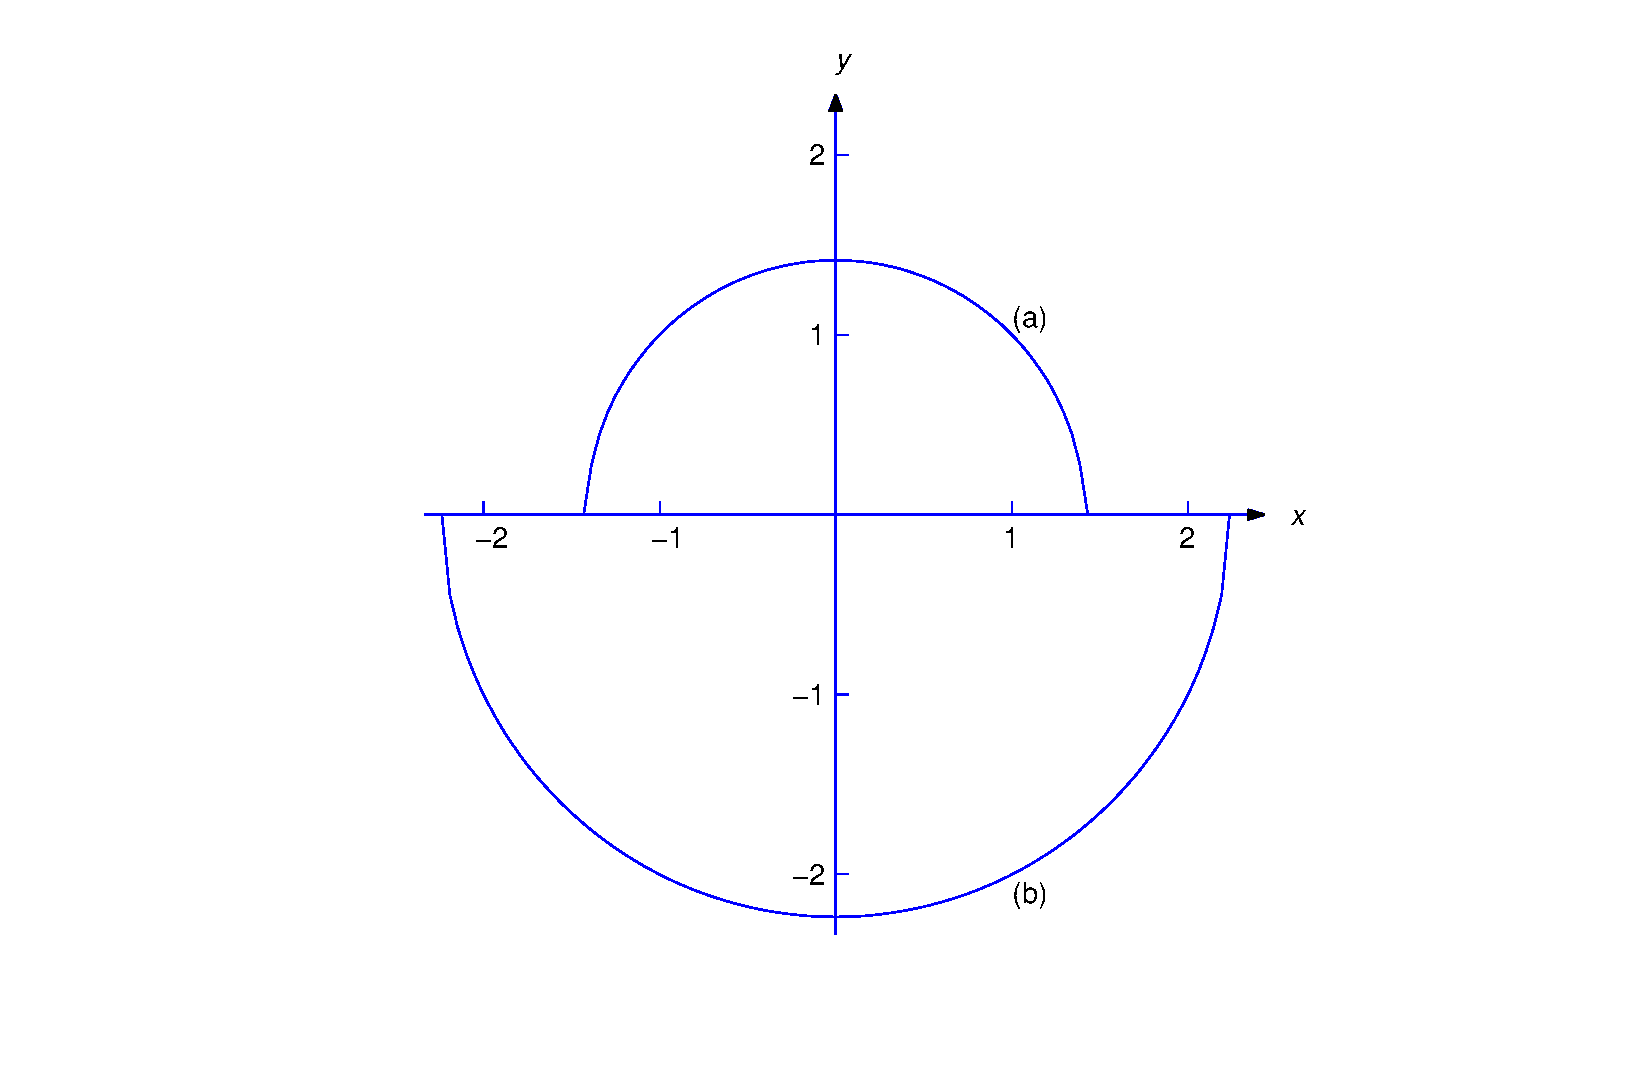
\includegraphics[bb=-78 148 689 643,width=5.67in,height=3.66in,keepaspectratio]{fig020201}
\color{blue}
  \caption{
{\bf (a)} $y=\sqrt{2-x^{2}}$,\, $-\sqrt{2}<x<\sqrt{2}$; \,
{\bf (b)} $y=-\sqrt{5-x^{2}}$,\, $-\sqrt{5}<x<\sqrt{5}$}
  \label{figure:2.2.1}
\end{figure}


\boxit{Implicit Solutions of Separable Equations}


\noindent
In Examples~\ref{example:2.2.1} and \ref{example:2.2.2} we were able to
solve the equation $H(y)=G(x)+c$ to obtain explicit formulas for
solutions of the given separable differential equations. As we'll
see in the next example, this isn't  always possible.
In this situation we must broaden our definition of a solution of a
separable equation. The next theorem provides the basis for this
modification.  We omit the proof, which requires a result from
advanced calculus called as the {\color{blue}\it implicit function
theorem\/}.

\begin{theorem}\color{blue}~\label{thmtype:2.2.1}
Suppose $g=g(x)$ is continous on $(a,b)$ and $h=h(y)$
are continuous on $(c,d).$ Let $G$ be an antiderivative of
$g$ on $(a,b)$ and let $H$ be an antiderivative of $h$ on $(c,d).$
Let $x_0$ be an arbitrary point in $(a,b),$ let $y_0$
be a point in $(c,d)$ such that $h(y_0)\ne0,$ and define
\begin{equation} \label{eq:2.2.10}
c=H(y_0)-G(x_0).
\end{equation}
Then there's a function $y=y(x)$ defined on some open interval
$(a_1,b_1),$ where $a\le a_1<x_0<b_1\le b,$ such that  $y(x_0)=y_0$
and
\begin{equation} \label{eq:2.2.11}
H(y)=G(x)+c
\end{equation}
for $a_1<x<b_1$.
Therefore $y$ is a solution of the initial value problem
\begin{equation} \label{eq:2.2.12}
h(y)y'=g(x),\quad y(x_0)=x_0.
\end{equation}
\end{theorem}


It's convenient to say that \eqref{eq:2.2.11} with $c$ arbitrary is an
{\color{blue}\it implicit solution\/} of $h(y)y'=g(x)$. Curves defined by
\eqref{eq:2.2.11} are integral curves of $h(y)y'=g(x)$. If $c$ satisfies
\eqref{eq:2.2.10}, we'll say that \eqref{eq:2.2.11} is an {\color{blue}\it
implicit
solution of the initial value problem\/} \eqref{eq:2.2.12}. However, keep
these  points in mind:
\begin{itemize}
\item  For some choices of $c$ there may not be any differentiable
functions $y$ that satisfy \eqref{eq:2.2.11}.
\item  The function $y$ in \eqref{eq:2.2.11} (not \eqref{eq:2.2.11} itself)
is a solution of $h(y)y'=g(x)$.
\end{itemize}

\begin{example}\label{example:2.2.3} \rm \mbox{}\newline
\begin{alist}
\item % (a)
Find implicit solutions of
\begin{equation} \label{eq:2.2.13}
y'={2x+1\over5y^4+1}.
\end{equation}
\item % (b)
Find an implicit solution of
\begin{equation} \label{eq:2.2.14}
y'={2x+1\over5y^4+1},\quad y(2)=1.
\end{equation}
\end{alist}
\end{example}

\solutionpart{a}
 Separating variables yields
$$
(5y^4+1)y'=2x+1.
$$
Integrating yields the implicit solution
\begin{equation} \label{eq:2.2.15}
y^5+y=x^2+x+ c.
\end{equation}
of \eqref{eq:2.2.13}.

\solutionpart{b} Imposing the initial condition $y(2)=1$ in
\eqref{eq:2.2.15} yields $1+1=4+2+c$, so $c=-4$. Therefore
$$
y^5+y=x^2+x-4
$$
is an implicit solution of the initial value problem \eqref{eq:2.2.14}.
Although more than one differentiable function $y=y(x)$ satisfies
\ref{eq:2.2.13}) near $x=1$, it can be shown that there's only
one such function that satisfies the initial condition $y(1)=2$.

Figure~\ref{figure:2.2.2} shows a direction field and some integral curves
for \eqref{eq:2.2.13}.

\begin{figure}[tbp]
  \centering
  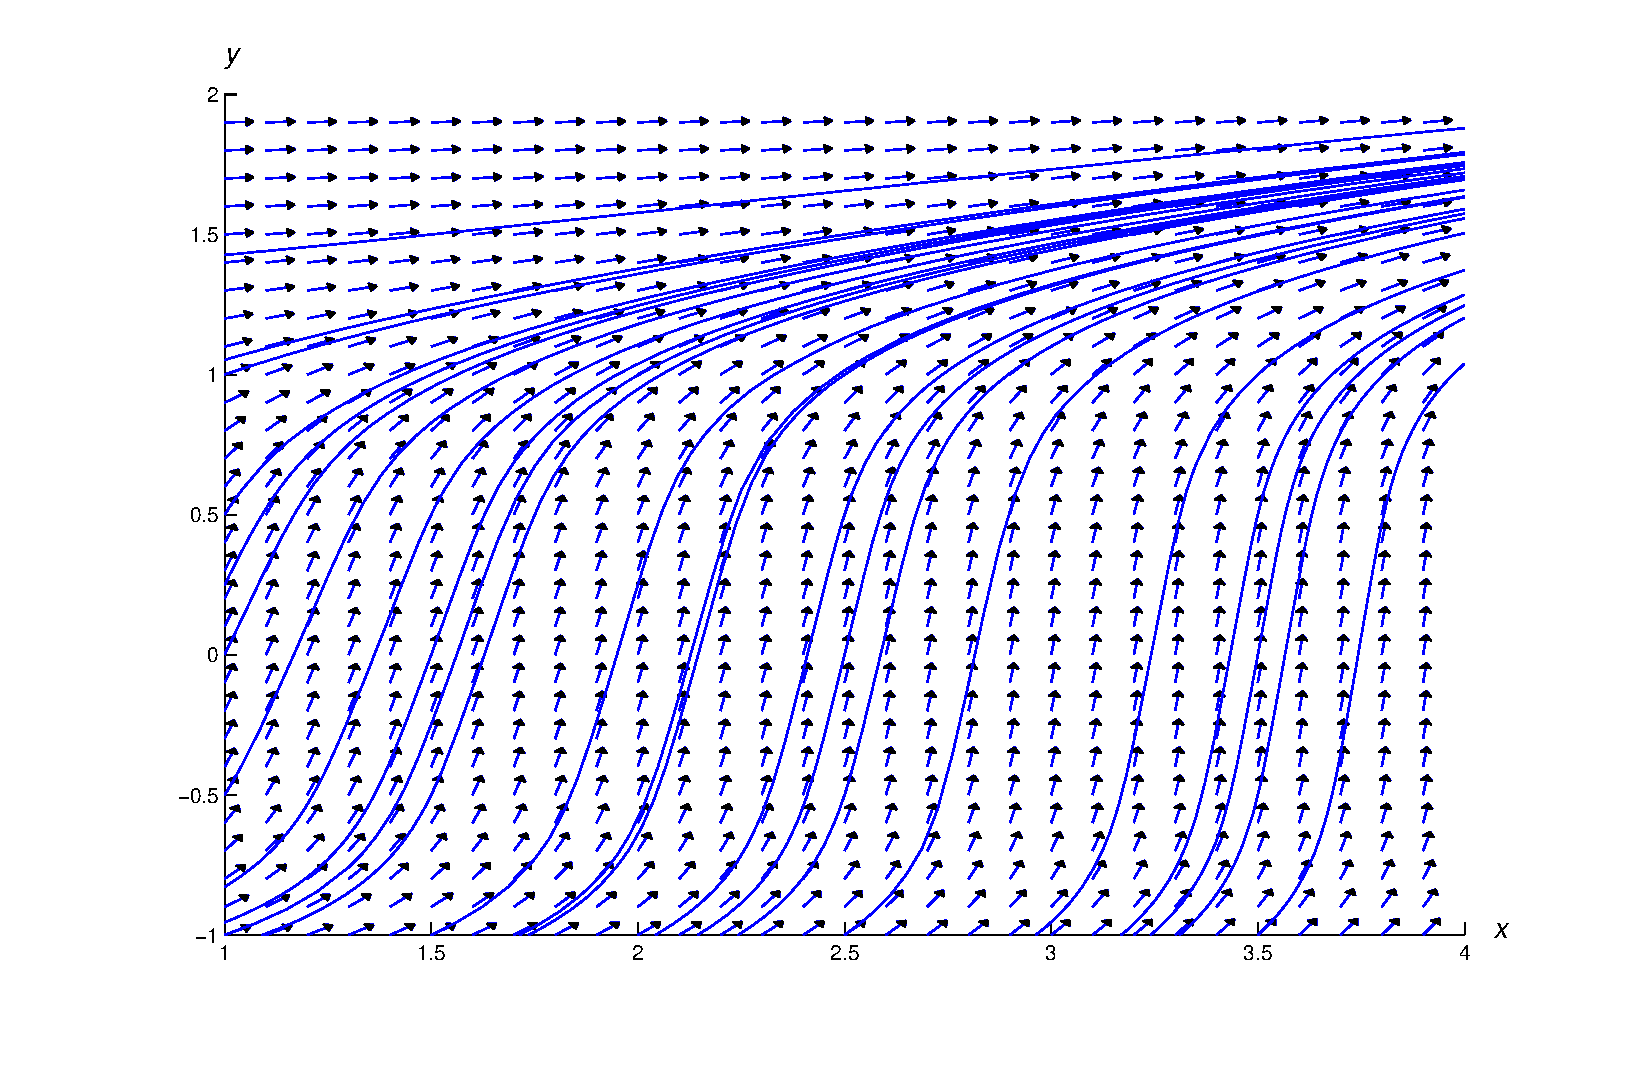
\includegraphics[bb=-78 148 689 643,width=5.67in,height=3.66in,keepaspectratio]{fig020202}
\color{blue}
  \caption{A direction field and integral curves for
$y'=\dst{\frac{2x+1}{5y^{4}+1}}$}
  \label{figure:2.2.2}
\end{figure}

\boxit{Constant Solutions of Separable Equations}

\noindent
An equation of the form
$$
y'=g(x)p(y)
$$
 is separable, since it can be rewritten as
$$
{1\over p(y)}y'=g(x).
$$
 However, the division by  $p(y)$
is not legitimate  if $p(y)=0$ for some values of $y$.  The
next two examples show how to deal with this problem.

\begin{example}\label{example:2.2.4}
\rm  Find all solutions of
\begin{equation} \label{eq:2.2.16}
y'=2xy^2.
\end{equation}
\end{example}
\solution Here we must divide by $p(y)=y^2$ to separate variables.
This isn't  legitimate if $y$ is a solution of \eqref{eq:2.2.16} that
equals zero for some value of $x$. One such solution can be found by
inspection:  $y \equiv 0$. Now suppose   $y$ is a solution
of \eqref{eq:2.2.16} that isn't  identically zero. Since $y$ is continuous
there must be an interval on which $y$ is never zero. Since division
by $y^2$ is legitimate for $x$ in this interval, we can separate
variables in \eqref{eq:2.2.16} to obtain
$$
{y'\over y^2}=2x.
$$
 Integrating this yields
$$
-{1\over y}=x^2+c,
$$
which is equivalent to
\begin{equation} \label{eq:2.2.17}
y=-{1\over x^2+c}.
\end{equation}


We've now shown that if $y$ is a solution of \eqref{eq:2.2.16} that is
not identically zero, then $y$ must be of the form \eqref{eq:2.2.17}. By
substituting \eqref{eq:2.2.17} into \eqref{eq:2.2.16}, you can verify that
\eqref{eq:2.2.17} is  a solution of \eqref{eq:2.2.16}. Thus,
 solutions of \eqref{eq:2.2.16} are $y\equiv0$ and the functions
of the form \eqref{eq:2.2.17}. Note that the solution $y\equiv0$ isn't  of
the form \eqref{eq:2.2.17} for any value of $c$.

Figure~\ref{figure:2.2.3} shows a direction field and some integral
curves for \eqref{eq:2.2.16}


\begin{figure}[tbp]
  \centering
  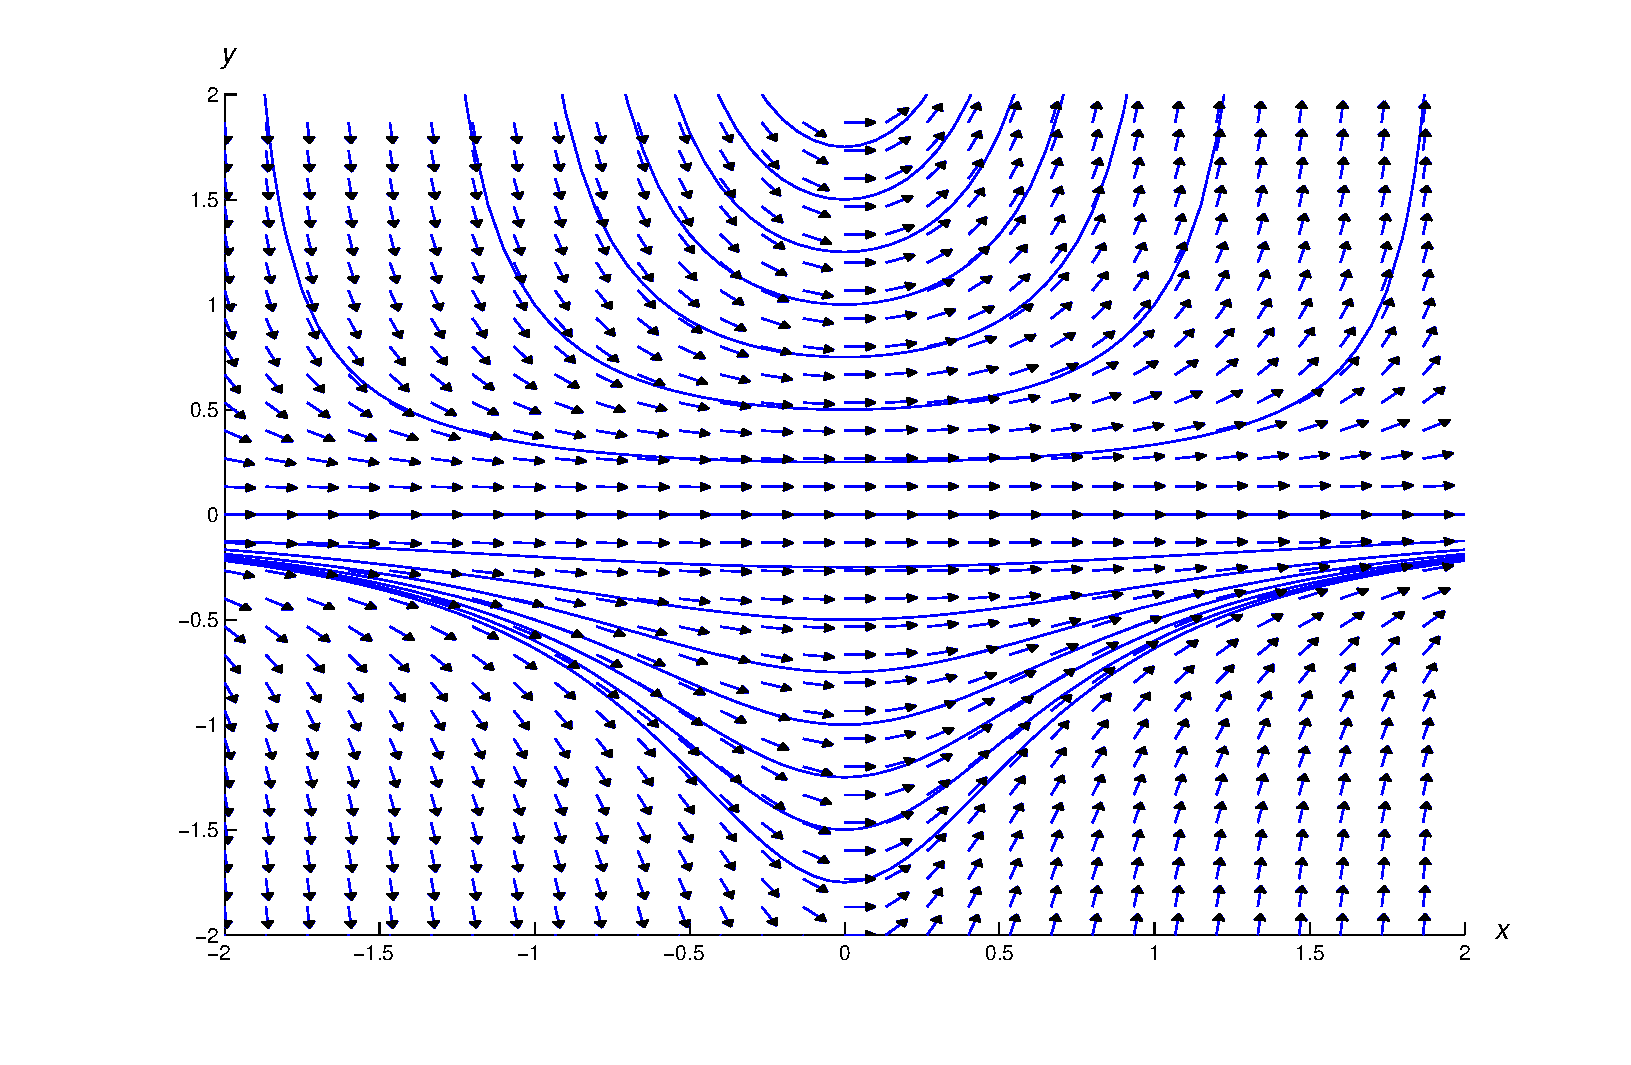
\includegraphics[bb=-78 148 689 643,width=5.67in,height=3.66in,keepaspectratio]{fig020203}
\color{blue}
  \caption{A direction field and  integral curves for $y'=2xy^{2}$}
  \label{figure:2.2.3}
\end{figure}

\begin{example}\label{example:2.2.5}
\rm  Find all solutions of
\begin{equation} \label{eq:2.2.18}
y'={1\over2}x(1-y^2).
\end{equation}
\end{example}

\solution Here we must divide by $p(y)=1-y^2$ to separate variables.
This isn't  legitimate if $y$ is a solution of \eqref{eq:2.2.18} that
equals $\pm1$ for some value of $x$. Two such solutions can be found
by inspection: $y \equiv 1$ and $y\equiv-1$. Now suppose
$y$ is a solution of \eqref{eq:2.2.18} such that $1-y^2$ isn't
identically zero. Since $1-y^2$ is continuous there must be an
interval on which $1-y^2$ is never zero. Since division by $1-y^2$ is
legitimate for $x$ in this interval, we can separate variables in
\eqref{eq:2.2.18} to obtain
$$
{2y'\over y^2-1}=-x.
$$
 A partial fraction expansion on the left yields
$$
\left[{1\over y-1}-{1\over y+1}\right]y'=-x,
$$
and integrating  yields
$$
\ln\left|{y-1\over y+1}\right|=-{x^2\over2}+k;
$$
 hence,
$$
\left|{y-1\over y+1}\right|=e^ke^{-x^2/2}.
$$
 Since $y(x)\ne\pm1$ for $x$ on the interval under discussion, the
quantity
$(y-1)/(y+1)$  can't  change sign in this interval. Therefore
we can rewrite the last equation as
$$
{y-1\over y+1}=ce^{-x^2/2},
$$
  where $c=\pm e^k$, depending upon the sign of $(y-1)/(y+1)$ on the
interval.
 Solving for  $y$ yields
\begin{equation} \label{eq:2.2.19}
y={1+ce^{-x^2/2}\over  1-ce^{-x^2/2}}.
\end{equation}

We've now shown that if $y$ is a solution of \eqref{eq:2.2.18} that  is
not identically equal to $\pm1$, then $y$ must be as in
\eqref{eq:2.2.19}. By substituting \eqref{eq:2.2.19} into \eqref{eq:2.2.18} you
 can verify that \eqref{eq:2.2.19} is  a solution of
\eqref{eq:2.2.18}. Thus,  the solutions of \eqref{eq:2.2.18}
are $y\equiv1$, $y\equiv-1$ and the functions of the form
\eqref{eq:2.2.19}. Note that the constant solution $y \equiv 1$ can be
obtained from this formula by taking $c=0$;     however, the other
constant solution, $y \equiv -1$, can't be obtained in this way.

Figure~\ref{figure:2.2.4} shows a direction field and some integrals for
\eqref{eq:2.2.18}.


\begin{figure}[H]
  \centering
  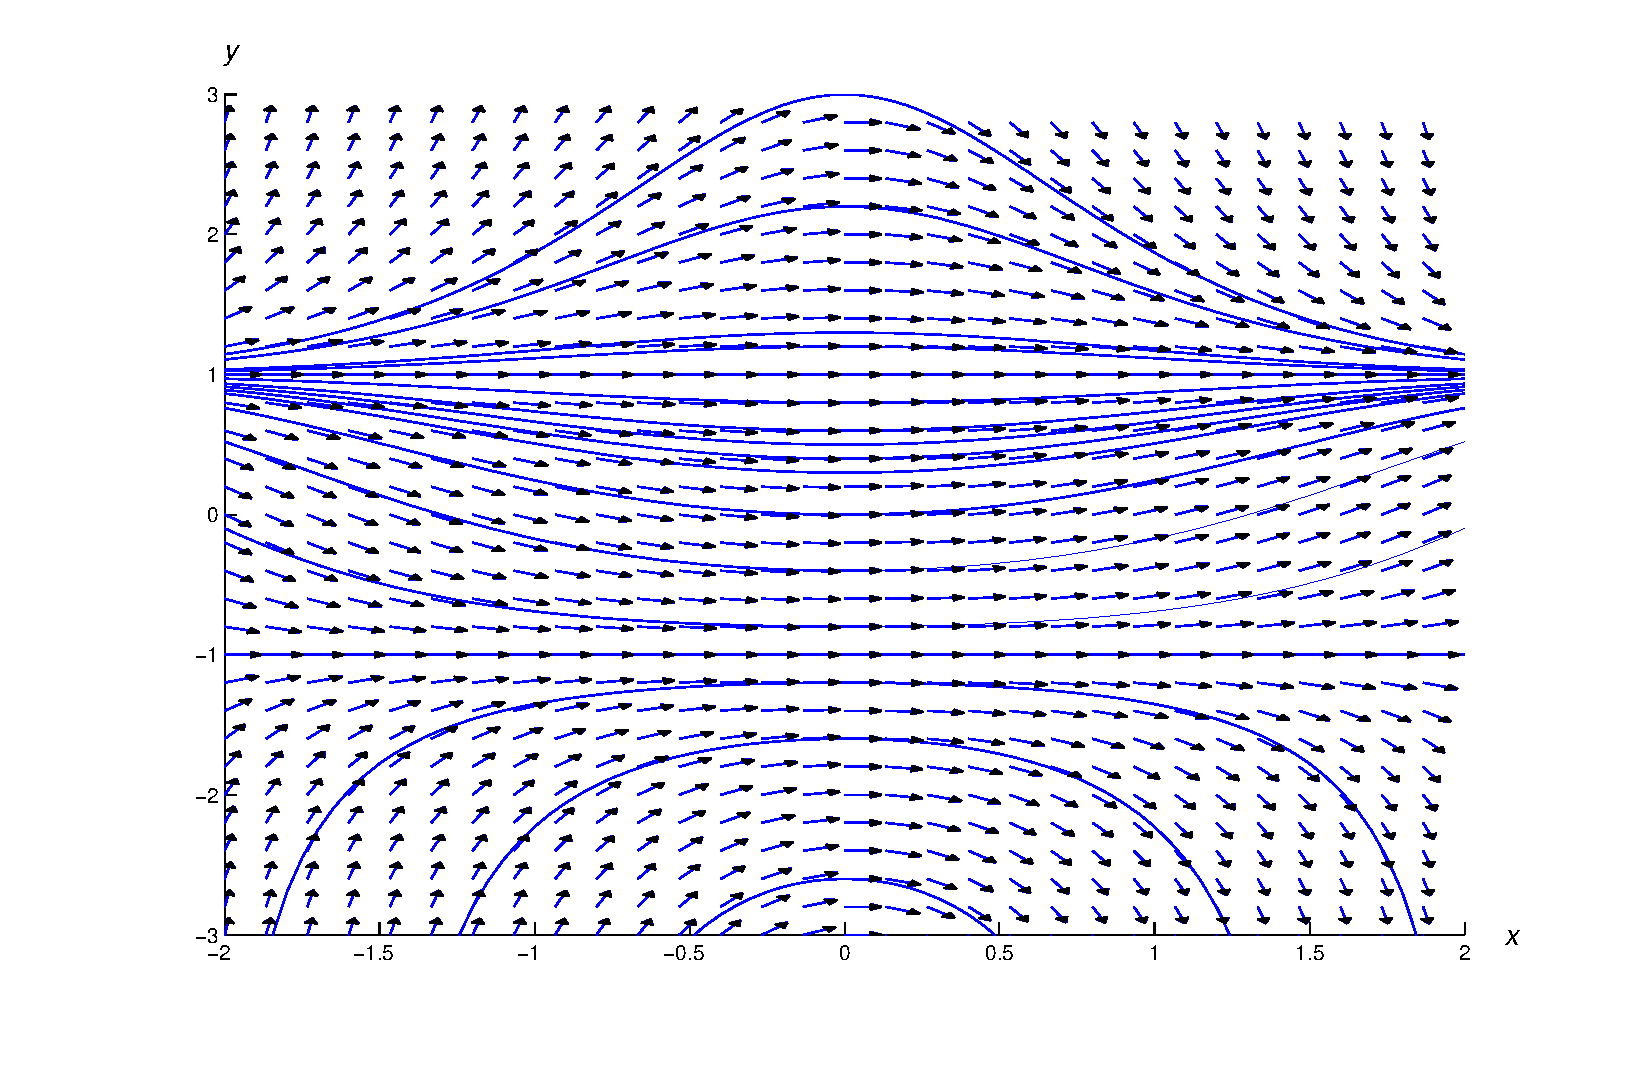
\includegraphics[bb=-78 148 689 643,width=5.67in,height=3.66in,keepaspectratio]{fig020204}
\color{blue}
\caption{
A direction field and integral curves for
$y'=\dst{\frac{x(1-y^2)}{2}}$}
  \label{figure:2.2.4}
\end{figure}

\boxit{Differences Between Linear and Nonlinear Equations}

\noindent
Theorem~\ref{thmtype:2.1.2} states that if $p$ and $f$ are continuous on
$(a,b)$ then every solution of
$$
y'+p(x)y=f(x)
$$
 on  $(a,b)$  can be obtained by choosing a value for the constant
$c$  in the general solution, and   if
$x_0$ is any point in  $(a,b)$ and $y_0$ is arbitrary, then the
initial value problem
$$
y'+p(x)y=f(x),\quad y(x_0)=y_0
$$
 has a solution on  $(a,b)$.

The not true for nonlinear equations. First, we
saw in Examples~\ref{example:2.2.4} and \ref{example:2.2.5} that a
nonlinear
equation may have solutions that can't be obtained by choosing a
specific value of a constant appearing in a one-parameter family of
solutions. Second, it is in general impossible to determine the
interval of validity of a solution to an initial value problem for a
nonlinear equation by simply examining the equation, since the
interval of validity may depend on the initial condition. For
instance, in Example~\ref{example:2.2.2} we saw that the solution of
$$
{dy\over dx}=-{x\over y},\quad y(x_0)=y_0
$$
is valid on $(-a,a)$, where $a=\sqrt{x_0^2+y_0^2}$.

\begin{example}\label{example:2.2.6}
\rm  Solve the initial value problem
$$
y'=2xy^2, \quad y(0)=y_0
$$
 and determine the  interval of validity of  the solution.
\end{example}


\solution  First suppose   $y_0\ne0$. From
Example~\ref{example:2.2.4}, we know that $y$ must be of the form
\begin{equation} \label{eq:2.2.20}
y=-{1\over x^2+c}.
\end{equation}
 Imposing the initial condition shows  that $c=-1/y_0$.
Substituting this into \eqref{eq:2.2.20} and rearranging terms yields
the solution
$$
y= {y_0\over 1-y_0x^2}.
$$
This is also the solution if $y_0=0$. If $y_0<0$,
the denominator isn't  zero for any value of $x$, so the
the solution is valid on $(-\infty,\infty)$. If $y_0>0$, the solution
 is  valid only on $(-1/\sqrt{y_0},1/\sqrt{y_0})$.

\exercises
 In Exercises \ref{exer:2.2.1}--\ref{exer:2.2.6} find all solutions.



\begin{exerciselist}
 \begin{tabular}[t]{
@{}p{168pt}@{}p{168pt}}
 \item\label{exer:2.2.1} $\dst{y'={3x^2+2x+1\over y-2}}$&
\item\label{exer:2.2.2}\vspace*{18pt} $(\sin x)(\sin y)+(\cos y)y'=0$
\end{tabular}

 \begin{tabular}[t]{@{}p{168pt}@{}p{168pt}}
\item\label{exer:2.2.3} $xy'+y^2+y=0$
& \item\label{exer:2.2.4} $y' \ln |y|+x^2y= 0$
\end{tabular}

\item\label{exer:2.2.5}
$\dst{(3y^3+3y \cos y+1)y'+{(2x+1)y\over 1+x^2}=0}$


\item\label{exer:2.2.6} $x^2yy'=(y^2-1)^{3/2}$

\exercisetext{In Exercises \ref{exer:2.2.7}--\ref{exer:2.2.10} find all
solutions. Also, plot a direction field and some integral curves on
the indicated rectangular region.}


\item\label{exer:2.2.7} \CGex $\dst{y'=x^2(1+y^2)};   \; \{-1\le x\le1,\
-1\le y\le1\}$


 \item\label{exer:2.2.8} \CGex$ y'(1+x^2)+xy=0 ;  \; \{-2\le x\le2,\ -1\le
y\le1\}$

\item\label{exer:2.2.9} \CGex $y'=(x-1)(y-1)(y-2);   \; \{-2\le x\le2,\
-3\le y\le3\}$


 \item\label{exer:2.2.10} \CGex $(y-1)^2y'=2x+3;   \; \{-2\le x\le2,\ -2\le
y\le5\}$

\exercisetext{In Exercises \ref{exer:2.2.11} and \ref{exer:2.2.12} solve
the initial value problem.}

\item\label{exer:2.2.11}
$\dst{y'={x^2+3x+2\over y-2}, \quad y(1)=4}$

\item\label{exer:2.2.12} $y'+x(y^2+y)=0, \quad y(2)=1$

\exercisetext{In Exercises \ref{exer:2.2.13}-\ref{exer:2.2.16} solve
the initial value problem and graph the solution.}

\item\label{exer:2.2.13} \CGex
$(3y^2+4y)y'+2x+\cos x=0, \quad y(0)=1$



\item\label{exer:2.2.14} \CGex
$\dst{y'+{(y+1)(y-1)(y-2)\over x+1}=0, \quad y(1)=0}$

\item\label{exer:2.2.15} \CGex $y'+2x(y+1)=0, \quad y(0)=2$


\item\label{exer:2.2.16} \CGex
$y'=2xy(1+y^2),\quad y(0)=1$

\exercisetext{In Exercises \ref{exer:2.2.17}--\ref{exer:2.2.23} solve the initial
value problem and find the interval of validity of the solution.}

\item\label{exer:2.2.17}
$y'(x^2+2)+ 4x(y^2+2y+1)=0, \quad y(1)=-1$

\item\label{exer:2.2.18}
$y'=-2x(y^2-3y+2), \quad y(0)=3$

 \begin{tabular}[t]{@{}p{168pt}@{}p{168pt}}
\item\label{exer:2.2.19} $\dst{y'={2x\over 1+2y},
\quad y(2)=0}$ & \item \vspace*{5.5pt}\label{exer:2.2.20} $y'=2y-y^2,
\quad y(0)=1$ \end{tabular}

\item\label{exer:2.2.21}
$x+yy'=0, \quad y(3) =-4$

\item\label{exer:2.2.22}
$y'+x^2(y+1)(y-2)^2=0, \quad y(4)=2$

\item\label{exer:2.2.23}
$(x+1)(x-2)y'+y=0, \quad y(1)=-3$

\item\label{exer:2.2.24} Solve $\dst{y'={(1+y^2)
\over (1+x^2)}}$ explicitly.
\hint{Use the identity
$\dst{\tan(A+B)={\tan A+\tan B\over1-\tan A\tan B}}$.}

\item\label{exer:2.2.25} Solve $\dst
{y'\sqrt{1-x^2}+\sqrt{1-y^2}=0}$ explicitly.
\hint{Use the identity
$\sin(A-B)=\sin A\cos B-\cos A\sin B$.}

\item\label{exer:2.2.26}
Solve $\dst{y'={\cos x\over \sin y},\quad y (\pi)={\pi\over2}}$
explicitly. \hint{Use the identity $\cos(x+\pi/2)=-\sin x$ and the
periodicity of the cosine.}

\item\label{exer:2.2.27}
Solve the initial value problem
$$
y'=ay-by^2,\quad y(0)=y_0.
$$
Discuss the behavior  of the solution if
\part{a} $y_0\ge0$; \part{b} $y_0<0$.

\item\label{exer:2.2.28}
 The population $P=P(t)$ of a  species satisfies
the logistic equation
$$
P'=aP(1-\alpha P)
$$
 and  $P(0)=P_0>0$.  Find $P$  for $t>0$, and  find
$\lim_{t\to\infty}P(t)$.



\item\label{exer:2.2.29}
An epidemic spreads through a population at a rate
proportional to the product of the number of people already infected
and the number of people susceptible, but not yet infected. Therefore,
 if $S$ denotes the total population of susceptible people and
$I=I(t)$ denotes the number of infected people at time $t$, then
$$
I'=rI(S-I),
$$
where $r$ is a positive constant. Assuming that $I(0)=I_0$,
find $I(t)$ for $t>0$, and show that
$\lim_{t\to\infty}I(t)=S$.

\item\label{exer:2.2.30}
\Lex
The result of Exercise~\ref{exer:2.2.29} is discouraging: if any
susceptible member of the group is
initially infected, then in the long run all susceptible members are
infected!
 On a more hopeful note, suppose   the disease spreads
according to the model of Exercise~\ref{exer:2.2.29}, but there's a
medication that cures the infected population at a rate proportional
to the number of infected individuals. Now the equation for the number
of infected individuals becomes
$$
I'=rI(S-I)-qI
\eqno{\rm(A)}
$$
where $q$ is a positive constant.
\begin{alist}
\item % (a)
Choose  $r$ and $S$ positive.
By plotting  direction fields and solutions of (A) on
suitable rectangular grids
$$
R=\{0\le t \le T,\ 0\le I \le d\}
$$
in the $(t,I)$-plane, verify that if $I$ is any solution of
(A) such that $I(0)>0$, then $\lim_{t\to\infty}I(t)=S-q/r$
if $q<rS$ and $\lim_{t\to\infty}I(t)=0$ if $q\ge rS$.
\item % (b)
To verify the experimental results of \part{a}, use separation of
variables to solve (A) with initial condition $I(0)=I_0>0$, and find
$\lim_{t\to\infty}I(t)$. \hint{There are three cases to consider:
\part{i} $q<rS$;     \part{ii}   $q>rS$;   \part{iii} $q=rS$.}
\end{alist}

\item\label{exer:2.2.31}
\Lex
Consider the differential equation
$$
y'=ay-by^2-q,
\eqno{\rm(A)}
$$
where $a$, $b$ are positive constants, and $q$ is an arbitrary
constant. Suppose  $y$ denotes a solution of this equation
that satisfies the initial condition $y(0)=y_0$.

\begin{alist}
\item % (a)
Choose  $a$ and $b$ positive and  $q<a^2/4b$.
By plotting  direction fields and solutions of (A) on
suitable rectangular grids
$$
R=\{0\le t \le T,\ c\le y \le d\}
\eqno{\rm(B)}
$$
in the $(t,y)$-plane,  discover that there are numbers $y_1$ and
$y_2$ with $y_1<y_2$ such that if $y_0>y_1$ then
$\lim_{t\to\infty}y(t)=y_2$, and if $y_0<y_1$ then $y(t)=-\infty$
for some finite value of~$t$. (What happens if $y_0=y_1$?)



\item % (b)
Choose $a$ and $b$ positive and $q=a^2/4b$. By plotting direction
fields
and solutions of (A) on suitable rectangular grids of the form (B),
discover that there's a number $y_1$ such that if $y_0\ge y_1$ then
$\lim_{t\to\infty}y(t)=y_1$, while if $y_0<y_1$ then  $y(t)=-\infty$
for some finite value of $t$.

\item % (c)
Choose positive $a$, $b$ and $q>a^2/4b$. By plotting direction fields
and solutions of (A) on suitable rectangular grids of the form (B),
discover that
no matter what $y_0$ is, $y(t)=-\infty$ for some finite value of $t$.



\item % (d)
Verify your results experiments analytically.
Start by separating variables in (A)  to obtain
$$
{y'\over ay-by^2-q}=1.
$$
To decide what to do next you'll have to use the
quadratic formula. This should lead you to see why there are
three cases.  Take it from there!

Because of its role in the transition between these
three cases,  $q_0=a^2/4b$ is called a {\color{blue}\it bifurcation value\/}
of $q$. In general, if $q$ is a parameter in any differential
equation,  $q_0$ is said to be a bifurcation value of
$q$ if the nature of the solutions of the equation with $q<q_0$
is qualitatively different from the nature of the solutions
with $q>q_0$.
\end{alist}

\item\label{exer:2.2.32} \Lex
By plotting direction fields and solutions of
$$
y'=qy-y^3,
$$
convince yourself that $q_0=0$ is a bifurcation value of $q$
for this equation. Explain what makes you draw this conclusion.

\item\label{exer:2.2.33}
Suppose a disease spreads according to the model of
Exercise~\ref{exer:2.2.29}, but
there's a medication that cures the infected population at a constant
rate of $q$ individuals per unit  time, where $q>0$.
Then
the equation for the number of infected individuals becomes
$$
I'=rI(S-I)-q.
$$
Assuming that $I(0)=I_0>0$, use the results of
Exercise~\ref{exer:2.2.31} to describe what happens as $t\to\infty$.

\item\label{exer:2.2.34}
Assuming that $p \not\equiv 0$, state conditions under which the linear
equation
$$
y'+p(x)y=f(x)
$$
is separable.  If the equation satisfies these conditions, solve it by
separation of variables and by the method developed in
Section~2.1.

\exercisetext{Solve the equations in
Exercises~\ref{exer:2.2.35}--\ref{exer:2.2.38} using variation of
parameters followed by separation of variables.}

 \begin{tabular}[t]{@{}p{168pt}@{}p{168pt}}
\item\label{exer:2.2.35} $\dst{y'+y={2xe^{-x}\over1+ye^x}}$&
\item\label{exer:2.2.36}\vspace*{7pt}  $\dst{xy'-2y={x^6\over y+x^2}}$
\end{tabular}

 \begin{tabular}[t]{@{}p{168pt}@{}p{168pt}}
\item\label{exer:2.2.37} $\dst{y'-y}={(x+1)e^{4x}\over(y+e^x)^2}$&
\item\label{exer:2.2.38} $y'-2y=\dst{xe^{2x}\over1-ye^{-2x}}$
\end{tabular}


\item\label{exer:2.2.39}
Use variation of parameters to show that the solutions of the
following equations are of the form $y=uy_1$, where $u$ satisfies a
separable equation $u'=g(x)p(u)$. Find $y_1$ and $g$ for each
equation.

\begin{tabular}[t]{@{}p{168pt}@{}p{168pt}}
{\bf (a)} $xy'+y=h(x)p(xy)$
& {\bf (b)} $\dst{xy'-y=h(x) p\left({y\over x}\right)}$\\[2\jot]
{\bf (c)} $y'+y=h(x) p(e^xy)$
& {\bf (d)} $xy'+ry=h(x) p(x^ry)$\\[2\jot]
{\bf (e)} $\dst{y'+{v'(x)\over v(x)}y= h(x)
p\left(v(x)y\right)}$
\end{tabular}
\end{exerciselist}

\newsection{3}{First Order Equations} {Existence and Uniqueness of Solutions of Nonlinear Equations}
\currentpdfbookmark{Section 2.3 Existence and Uniqueness of Solutions of Nonlinear Equations}{section:2.3}
\vskip14pt
\renewcommand{\thissection}{\sectiontitle{\,
EXISTENCE AND UNIQUENESS OF SOLUTIONS OF NONLINEAR EQUATIONS}}
\thissection



\noindent
Although  there are  methods for
 solving some nonlinear equations, it's
impossible to find  useful formulas for the solutions of most.
Whether we're looking for  exact solutions or numerical
approximations, it's useful to know  conditions that imply the
existence and uniqueness of solutions of initial value problems for
nonlinear equations. In this section we state  such a condition and
illustrate it with examples.



\vspace*{-15pt}
\begin{figure}[H]
  \centering
\scalebox{.9}{
  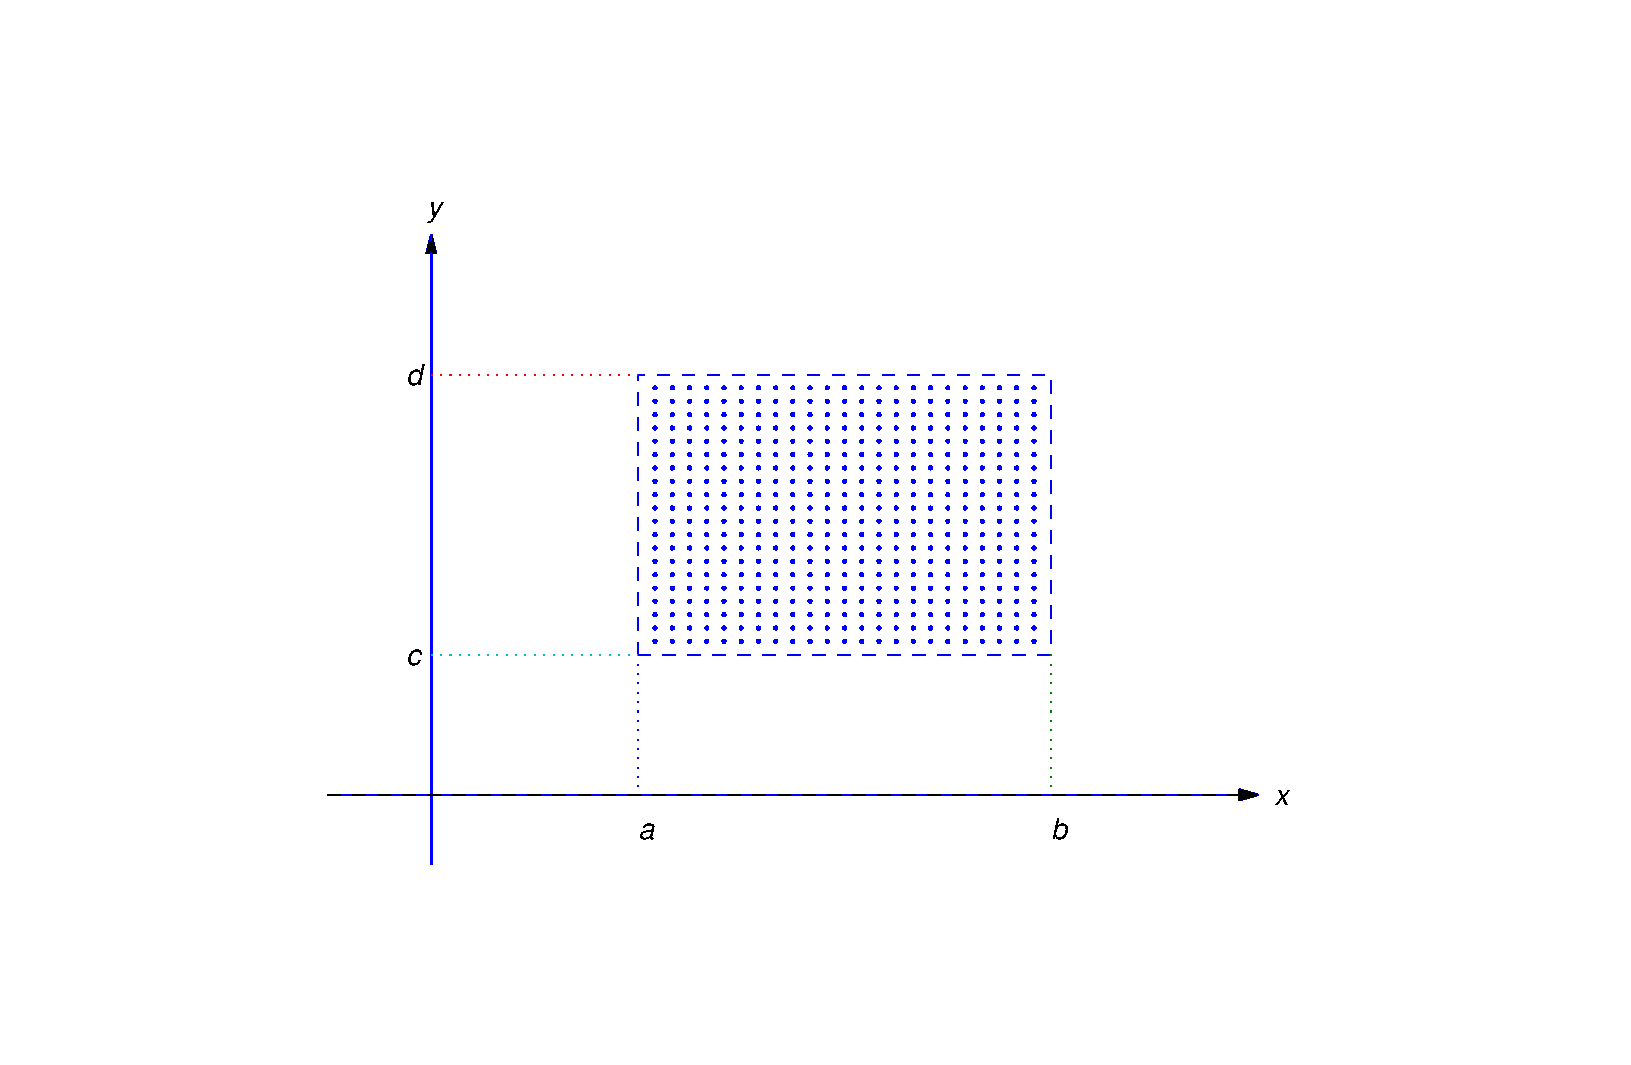
\includegraphics[bb=-78 148 689 643,width=5.67in,height=3.66in,keepaspectratio]{fig020301}}
\color{blue}
\vspace*{-35pt}
  \caption{An open rectangle}
  \label{figure:2.3.1}
\end{figure}


Some terminology:
 an {\color{blue}\it open rectangle $R$\/}
 is a set of points $(x,y)$ such that
$$
a<x<b\mbox{\quad  and \quad}c<y<d
$$
 (Figure~\ref{figure:2.3.1}).  We'll denote this set by
$R:  \{ a < x < b, c < y < d \}$.
 ``Open'' means that the
boundary rectangle (indicated by the dashed lines in
Figure~\ref{figure:2.3.1}) isn't  included in  $R$ .

The next theorem gives sufficient conditions for existence and
uniqueness of solutions of initial value problems for first order
nonlinear differential equations. We omit the proof, which is beyond
the scope of this book.

\begin{theorem}\color{blue} \label{thmtype:2.3.1} \mbox{}\newline
\vspace*{-5pt}
\begin{alist}
\item %(a)
 If  $f$ is continuous
on an open rectangle
$$
R:  \{ a < x < b, c < y < d \}
$$
 that contains $(x_0,y_0)$
then  the initial value problem
\begin{equation} \label{eq:2.3.1}
y'=f(x,y), \quad y(x_0)=y_0
\end{equation}
 has at least one solution  on some open subinterval
of  $(a,b)$ that contains $x_0.$

\item % (b)
 If  both $f$ and  $f_y$ are
 continuous on $R$ then \eqref{eq:2.3.1} has a unique
solution on some open subinterval  of $(a,b)$ that contains $x_0$.
\end{alist}
\end{theorem}


It's important to understand exactly what Theorem~\ref{thmtype:2.3.1}
says.

\begin{itemize}
\item \part{a} is an {\color{blue}\it existence theorem\/}. It guarantees that a
solution exists on some open interval that contains $x_0$, but provides
no information on how to find the solution, or to determine the open
interval on which it exists. Moreover, \part{a} provides no
information on the number of solutions that \eqref{eq:2.3.1} may have. It
leaves open the possibility that \eqref{eq:2.3.1} may have two or more
solutions that differ for values of $x$ arbitrarily close to $x_0$. We
will see in Example~\ref{example:2.3.6} that this can happen.

\item \part{b} is a {\color{blue}\it uniqueness theorem\/}. It guarantees that
\eqref{eq:2.3.1} has a unique solution on some open interval (a,b) that
contains $x_0$. However, if $(a,b)\ne(-\infty,\infty)$,
\eqref{eq:2.3.1} may have more than one solution on a larger interval
that contains $(a,b)$. For example, it may happen that $b<\infty$ and all
solutions have the same values on $(a,b)$, but two solutions $y_1$ and
$y_2$ are defined on some interval $(a,b_1)$ with $b_1>b$, and have
different values for $b<x<b_1$;   thus, the graphs of the $y_1$ and
$y_2$ ``branch off'' in different directions at $x=b$. (See
Example~\ref{example:2.3.7} and Figure~\ref{figure:2.3.3}). In this case,
continuity implies that $y_1(b)=y_2(b)$ (call their common value
$\overline y$), and  $y_1$ and $y_2$ are both solutions of the initial
value problem
\begin{equation} \label{eq:2.3.2}
y'=f(x,y),\quad y(b)=\overline y
\end{equation}
that differ on every open interval that contains $b$. Therefore
$f$ or $f_y$ must have a discontinuity at some point in each open
rectangle that contains $(b,\overline y)$, since if this were not so,
\eqref{eq:2.3.2} would have a unique solution on some open interval
that contains $b$. We leave it to you to give a similar analysis of the
case where $a>-\infty$.
 \end{itemize}

\begin{example}\label{example:2.3.1}
\rm   Consider  the initial value problem
\begin{equation} \label{eq:2.3.3}
y'={x^2-y^2 \over 1+x^2+y^2}, \quad y(x_0)=y_0.
\end{equation}
Since
$$
f(x,y)  = {x^2-y^2 \over 1+x^2+y^2}\mbox{\quad and \quad}
f_y(x,y)  =  -{2y(1+2x^2)\over (1+x^2+y^2)^2}
$$
are continuous for all $(x,y)$, Theorem~\ref{thmtype:2.3.1} implies that
if $(x_0,y_0)$ is arbitrary, then
\eqref{eq:2.3.3} has a unique solution on some open interval that contains
$x_0$.
\end{example}


\begin{example}\label{example:2.3.2}
\rm  Consider  the initial value problem
\begin{equation} \label{eq:2.3.4}
y'={x^2-y^2 \over x^2+y^2}, \quad y(x_0)=y_0.
\end{equation}
Here
$$
f(x,y)  =  {x^2-y^2 \over x^2+y^2}\mbox{\quad and \quad}
f_y(x,y)  =  \dst -{4x^2y \over (x^2+y^2)^2}
$$
are continuous everywhere except at $(0,0)$. If $(x_0,y_0)
\ne(0,0)$, there's an open rectangle $R$ that contains
$(x_0,y_0)$ that does not contain $(0,0)$. Since $f$ and $f_y$ are
continuous on $R$, Theorem~\ref{thmtype:2.3.1} implies that if
$(x_0,y_0)\ne(0,0)$ then
\eqref{eq:2.3.4}
has a unique solution on some open interval that contains $x_0$.
\end{example}

\begin{example}\label{example:2.3.3}
\rm  Consider the initial value problem
\begin{equation} \label{eq:2.3.5}
y'={x+y\over x-y},\quad y(x_0)=y_0.
\end{equation}
Here
$$
f(x,y)  =  {x+y\over x-y}\mbox{\quad and \quad}
f_y(x,y)  =  {2x\over (x-y)^2}
$$
are continuous everywhere except on the line $y=x$. If $y_0\ne x_0$,
there's an open rectangle $R$ that contains $(x_0,y_0)$ that
does not intersect the line $y=x$. Since $f$ and $f_y$ are continuous
on $R$, Theorem~\ref{thmtype:2.3.1} implies that if $y_0\ne x_0$,
\eqref{eq:2.3.5} has a unique solution on some open interval that contains
$x_0$.
\end{example}

\begin{example}\label{example:2.3.4}
\rm In Example~\ref{example:2.2.4} we saw that the
solutions of
\begin{equation} \label{eq:2.3.6}
y'=2xy^2
\end{equation}
are
 $$
y\equiv0\mbox{\quad and \quad} y=-{1 \over x^2+c},
$$
where $c$ is an arbitrary constant. In particular, this implies that
no solution of \eqref{eq:2.3.6} other than $y\equiv0$ can equal zero for
any value of $x$. Show that Theorem~\ref{thmtype:2.3.1}\part{b} implies
this.
\end{example}

\solution
We'll obtain a contradiction
by assuming that \eqref{eq:2.3.6} has a solution $y_1$ that equals
zero for some value of $x$, but isn't  identically zero. If $y_1$
has this property,  there's a point $x_0$ such that $y_1(x_0)=0$,
but $y_1(x)\ne0$ for some value of $x$ in every open interval that contains
$x_0$. This means that the initial value problem
\begin{equation} \label{eq:2.3.7}
y'=2xy^2,\quad y(x_0)=0
\end{equation}
has two solutions $y\equiv0$ and $y=y_1$ that differ for some value of
$x$ on every open interval that contains $x_0$. This contradicts
Theorem~\ref{thmtype:2.3.1}(b), since in \eqref{eq:2.3.6} the functions
$$
f(x,y)=2xy^2 \mbox{\quad and \quad} f_y(x,y)= 4xy.
$$
are both continuous
for all $(x,y)$, which implies that \eqref{eq:2.3.7} has a unique
solution on some open interval that contains $x_0$.

\begin{example}\label{example:2.3.5}
\rm  Consider the initial value problem
\begin{equation} \label{eq:2.3.8}
y' = {10\over 3}xy^{2/5}, \quad y(x_0) = y_0.
\end{equation}
\begin{alist}
\item %(a)
For what points $(x_0,y_0)$ does Theorem~\ref{thmtype:2.3.1}\part{a}
imply that
\eqref{eq:2.3.8} has a solution?

\item %(b)
For what points $(x_0,y_0)$ does Theorem~\ref{thmtype:2.3.1}\part{b}
imply that
\eqref{eq:2.3.8} has a  unique solution on some open interval that contains
$x_0$?
\end{alist}
\end{example}

\solutionpart{a} Since
$$
f(x,y) = {10\over 3}xy^{2/5}
$$
is continuous for all $(x,y)$,  Theorem~\ref{thmtype:2.3.1}
implies that \eqref{eq:2.3.8} has a solution for every $(x_0,y_0)$.

\solutionpart{b} Here
$$
f_y(x,y) = {4 \over 3}xy^{-3/5}
$$
is continuous for all $(x,y)$ with $y\ne 0$. Therefore, if $y_0\ne0$
there's an open rectangle on which both $f$ and $f_y$ are
continuous, and Theorem~\ref{thmtype:2.3.1} implies that \eqref{eq:2.3.8} has
a unique solution on some open interval that contains $x_0$.

If $y=0$ then $f_y(x,y)$ is undefined, and therefore discontinuous;
hence, Theorem~\ref{thmtype:2.3.1} does not apply to \eqref{eq:2.3.8} if
$y_0=0$.

\begin{example}\label{example:2.3.6}
\rm  Example~\ref{example:2.3.5} leaves open the possibility  that the
initial value problem
\begin{equation} \label{eq:2.3.9}
y'={10 \over 3}xy^{2/5}, \quad y(0)=0
\end{equation}
has more than one solution on every open interval that contains $x_0=0$.  Show
that this is true.
\end{example}

\solution
By inspection, $y\equiv0$ is a solution of the
differential equation
\begin{equation} \label{eq:2.3.10}
y'={10 \over 3} xy ^{2/5}.
\end{equation}
 Since $y\equiv0$ satisfies the initial condition $y(0)=0$,
it's a solution of \eqref{eq:2.3.9}.

Now suppose  $y$ is a solution of \eqref{eq:2.3.10} that isn't
identically zero.
 Separating variables in \eqref{eq:2.3.10} yields
$$
 y^{-2/5}y'={10 \over 3}x
$$
on any open interval where $y$ has no zeros.
 Integrating this and rewriting the arbitrary constant as $5c/3$ yields
$$
{5\over 3}y^{3/5} = {5\over 3}(x^2+c).
$$
Therefore
\begin{equation} \label{eq:2.3.11}
y = (x^2+c)^{5/3}.
\end{equation}

Since we divided by $y$ to separate variables in \eqref{eq:2.3.10}, our
derivation of \eqref{eq:2.3.11} is legitimate only on open intervals where $y$
has no zeros. However, \eqref{eq:2.3.11} actually defines $y$ for all $x$,
and differentiating \eqref{eq:2.3.11} shows that
$$
y'={10 \over 3}x(x^2+c)^{2/3}={10 \over 3}xy^{2/5},\,-\infty<x<\infty.
$$
Therefore \eqref{eq:2.3.11} satisfies \eqref{eq:2.3.10} on
$(-\infty,\infty)$
even if $c\le 0$, so that $y(\sqrt{|c|})=y(-\sqrt{|c|})=0$. In
particular, taking $c=0$ in \eqref{eq:2.3.11} yields
$$
y=x^{10/3}
$$
as a second solution of \eqref{eq:2.3.9}.
 Both solutions are defined on
$(-\infty,\infty)$, and they differ on every
open interval that contains $x_0=0$ (see Figure~\ref{figure:2.3.2}.)
In fact, there are {\color{blue}\it four\/} distinct solutions of
\eqref{eq:2.3.9}  defined on $(-\infty,\infty)$ that differ
from each other on every open interval that contains $x_0=0$.
  Can you identify the other two?


\begin{figure}[tbp]
  \centering
  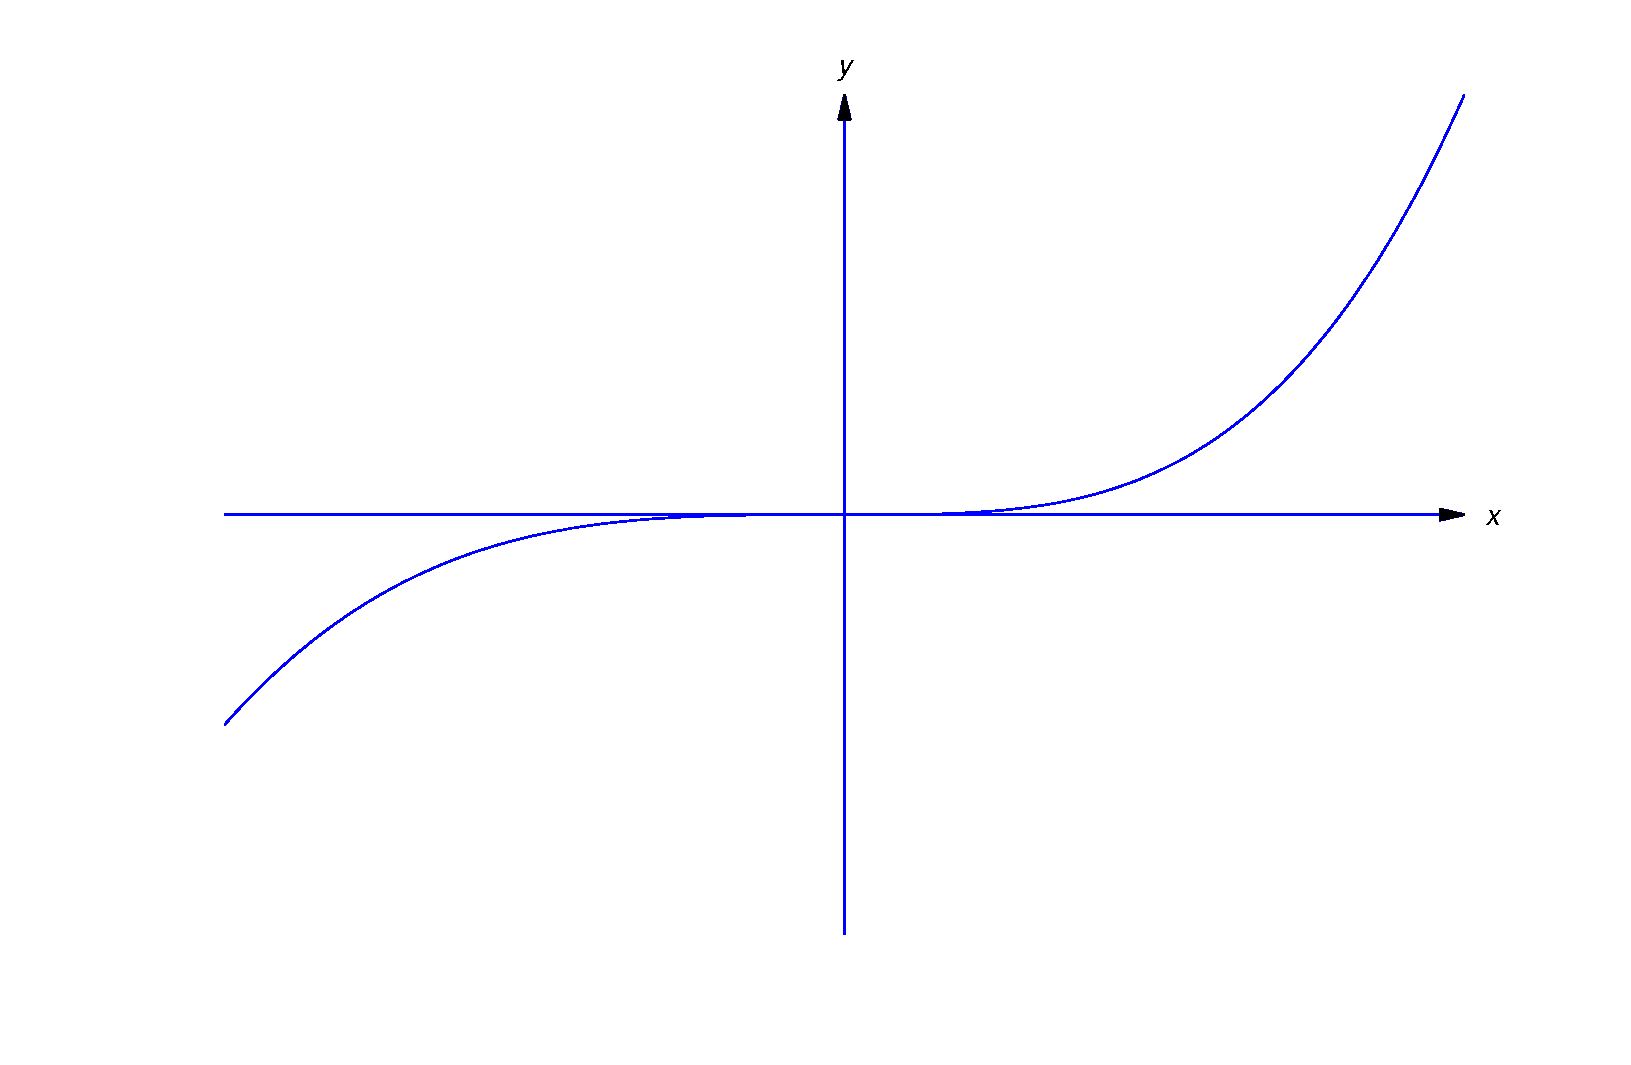
\includegraphics[bb=-78 148 689 643,width=5.67in,height=3.66in,keepaspectratio]{fig020302}
\color{blue}
\caption{Two solutions ($y=0$ and $y=x^{1/2}$) of \eqref{eq:2.3.9}  that
differ on every interval  containing $x_{0}=0$}
  \label{figure:2.3.2}
\end{figure}

\begin{example} \label{example:2.3.7}
\rm  From Example~\ref{example:2.3.5}, the initial value
problem
\begin{equation} \label{eq:2.3.12}
y'={10 \over 3}xy^{2/5}, \quad y(0)=-1
\end{equation}
 has a  unique solution on some open interval that contains $x_0=0$.
Find a solution and determine the largest open interval $(a,b)$ on
which it's unique.
\end{example}

\solution
Let $y$ be any solution of \eqref{eq:2.3.12}. Because of the initial
condition $y(0)=-1$ and the continuity of $y$, there's an open interval
$I$ that contains $x_0=0$ on which $y$ has no zeros, and is consequently
of the form \eqref{eq:2.3.11}. Setting $x=0$ and $y=-1$ in \eqref{eq:2.3.11}
yields $c=-1$, so
\begin{equation} \label{eq:2.3.13}
y=(x^2-1)^{5/3}
\end{equation}
for $x$  in $I$.
Therefore every solution of \eqref{eq:2.3.12} differs from zero
and is given by \eqref{eq:2.3.13} on $(-1,1)$; that is,
\eqref{eq:2.3.13} is the unique solution of \eqref{eq:2.3.12} on
$(-1,1)$.
 This is the largest open interval on which
\eqref{eq:2.3.12} has a unique solution. To see this, note that
\eqref{eq:2.3.13} is a solution of \eqref{eq:2.3.12} on $(-\infty,\infty)$.
From Exercise~2.2.~\hspace*{-3pt}\ref{exer:2.2.15}, there are infinitely many
other solutions
of \eqref{eq:2.3.12} that differ from \eqref{eq:2.3.13} on every open interval
larger than
$(-1,1)$. One such solution is
$$
y = \left\{ \begin{array}{cl}
(x^2-1)^{5/3}, & -1 \le x \le 1, \\[6pt]
0,             & |x|>1. \end{array} \right.
$$
(Figure \ref{figure:2.3.3}).



\begin{figure}[htbp]
\color{blue}
  \begin{minipage}[b]{0.5\linewidth}
    \centering
   \scalebox{.65}{
  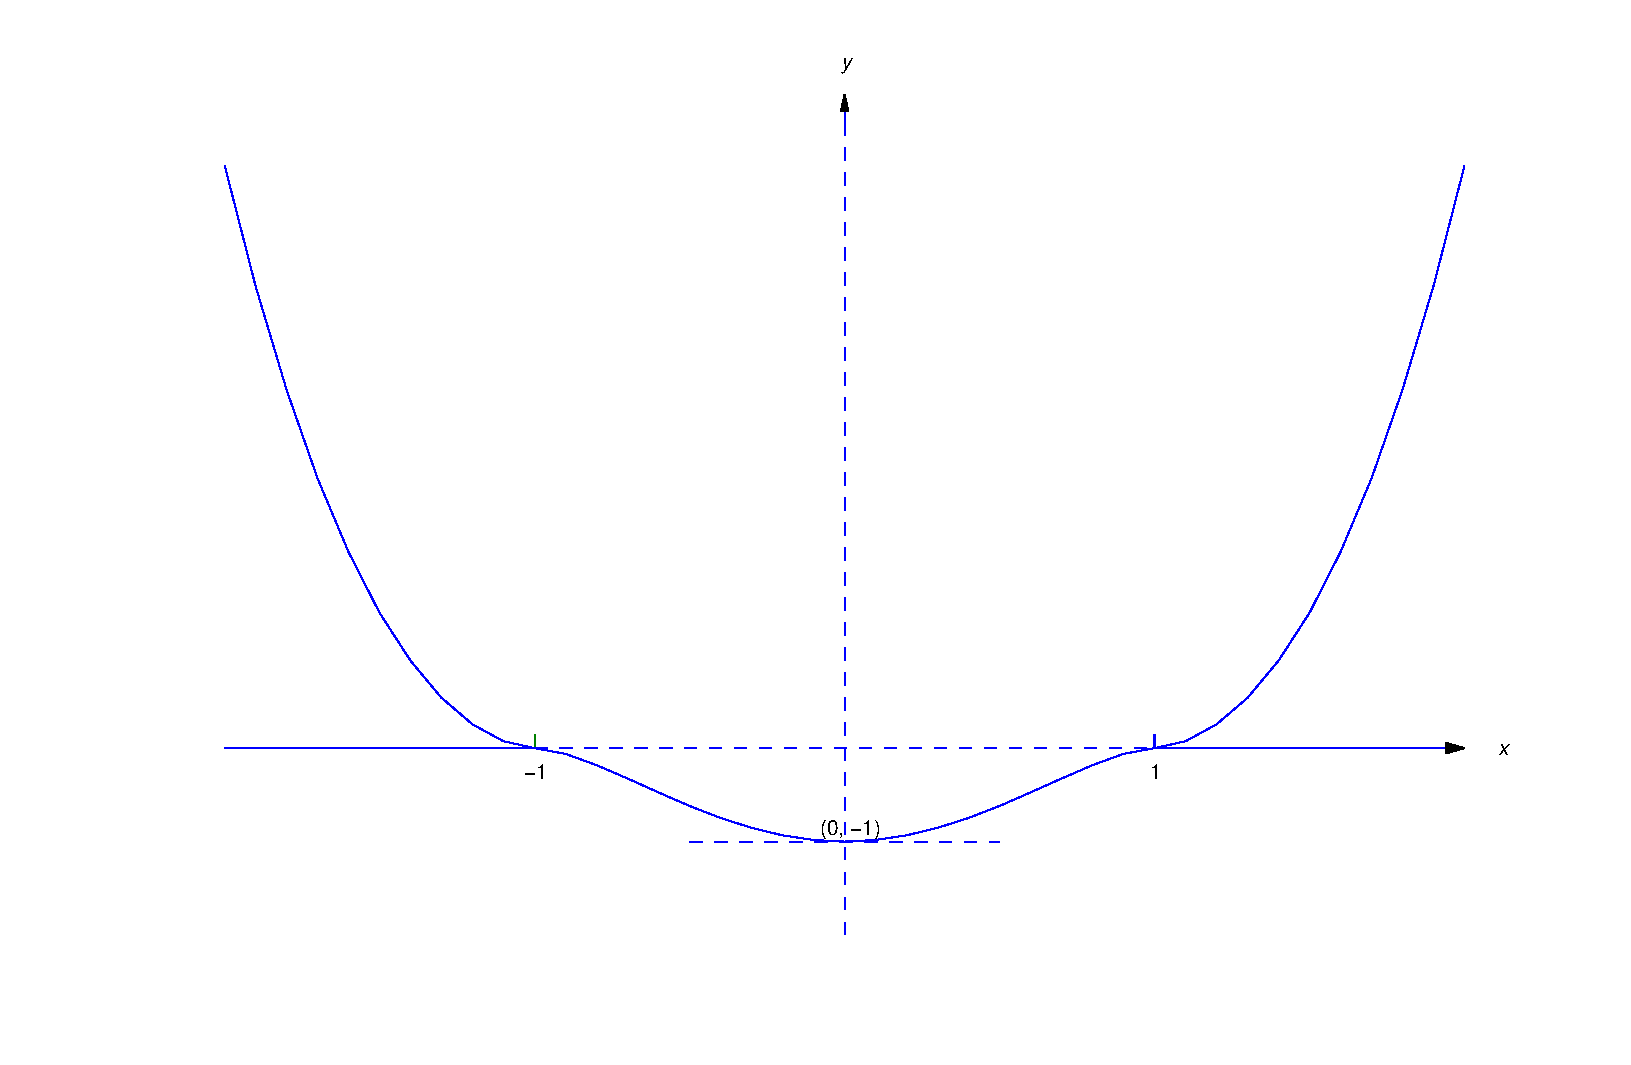
\includegraphics[bb=-78 148 689 643,width=5.67in,height=3.66in,keepaspectratio]{fig020303}}
\caption{ Two solutions of
\eqref{eq:2.3.12} on
$(-\infty,\infty)$ that coincide on $(-1,1)$, but on no larger open
interval}
  \label{figure:2.3.3}
  \end{minipage}
  \hspace{0.6cm}
  \begin{minipage}[b]{0.5\linewidth}
    \centering
   \scalebox{.65}{
  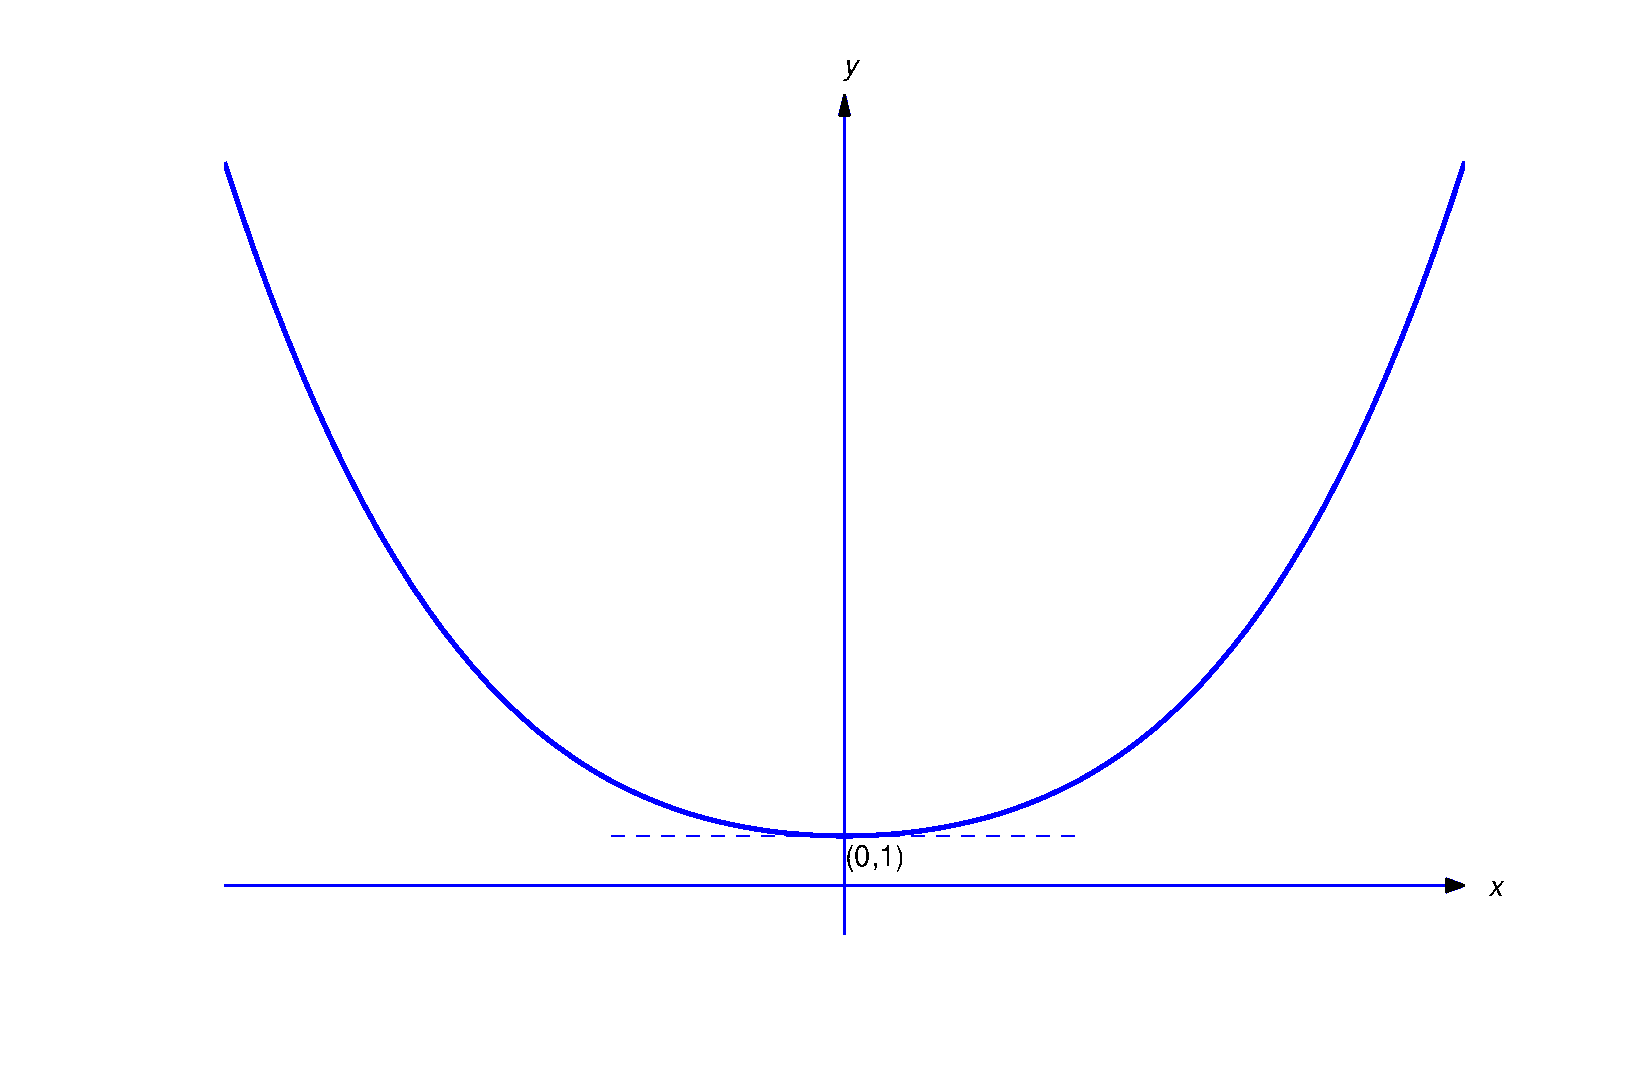
\includegraphics[bb=-78 148 689 643,width=5.67in,height=3.66in,keepaspectratio]{fig020304} }
  \caption{The unique solution of \eqref{eq:2.3.14}}
  \label{figure:2.3.4}
  \end{minipage}
\end{figure}


\begin{example}\label{example:2.3.8}
\rm  From Example~\ref{example:2.3.5}, the initial value
problem
\begin{equation} \label{eq:2.3.14}
y'={10 \over 3}xy^{2/5}, \quad y(0)=1
\end{equation}
 has a unique solution on some open interval that contains $x_0=0$.
Find the solution and determine the largest open interval on which it's
unique.
\end{example}

\solution
Let $y$ be any solution of \eqref{eq:2.3.14}. Because of the initial
condition $y(0)=1$ and the continuity of $y$, there's an open interval
$I$ that contains $x_0=0$ on which $y$ has no zeros, and is consequently
of the form \eqref{eq:2.3.11}. Setting $x=0$ and $y=1$ in \eqref{eq:2.3.11}
yields $c=1$, so
\begin{equation} \label{eq:2.3.15}
y=(x^2+1)^{5/3}
\end{equation}
for $x$ in $I$. Therefore every solution of \eqref{eq:2.3.14}
differs from zero and is given by \eqref{eq:2.3.15} on $(-\infty,\infty)$;
that is, \eqref{eq:2.3.15} is the unique solution of \eqref{eq:2.3.14} on
$(-\infty,\infty)$.
Figure~\ref{figure:2.3.4} shows the graph of this solution.

\exercises
 In Exercises \ref{exer:2.3.1}-\ref{exer:2.3.13} find all $(x_0,y_0)$ for
which Theorem~\ref{thmtype:2.3.1}
implies that the initial value problem $y'=f(x,y),\  y(x_0)=y_0$ has
\part{a}
a solution   \part{b} a  unique solution on some open interval that
contains
$x_0$.



\begin{exerciselist}

\begin{tabular}[t]{@{}p{168pt}@{}p{168pt}}
\item\label{exer:2.3.1} $\dst {y'={x^2+y^2
\over \sin
x}}$ &  \item\label{exer:2.3.2}\vspace*{10pt} $\dst
{y'={e^x+y \over x^2+y^2}}$ \end{tabular}

\begin{tabular}[t]{@{}p{168pt}@{}p{168pt}}
 \item\label{exer:2.3.3} $y'= \tan xy$
&  \item\label{exer:2.3.4} $\dst {y'={x^2+y^2
\over \ln xy}}$ \end{tabular}

\begin{tabular}[t]{@{}p{168pt}@{}p{168pt}}
 \item\label{exer:2.3.5} $y'=
(x^2+y^2)y^{1/3}$ &\  \item\label{exer:2.3.6}
\ $y'=2xy$ \end{tabular}

\begin{tabular}[t]{@{}p{168pt}@{}p{168pt}}
\vspace*{10pt} \item\label{exer:2.3.7} $\dst
{y'=\ln(1+x^2+y^2)}$
& \vspace*{4pt} \item\label{exer:2.3.8} $\dst {y'={2x+3y
\over x-4y}}$ \end{tabular}

\begin{tabular}[t]{@{}p{168pt}@{}p{168pt}}
 \item\label{exer:2.3.9} $\dst
{y'=(x^2+y^2)^{1/2}}$ &\item\label{exer:2.3.10}\  $y' =
x(y^2-1)^{2/3}$ \end{tabular}

\begin{tabular}[t]{@{}p{168pt}@{}p{168pt}}
\item\label{exer:2.3.11} $y'=(x^2+y^2)^2$
& \item\label{exer:2.3.12} $y'=(x+y)^{1/2}$
\end{tabular}


\item\label{exer:2.3.13}
$\dst {y'={\tan y \over x-1}}$

\item\label{exer:2.3.14}
Apply Theorem~\ref{thmtype:2.3.1} to the initial value problem
$$
y'+p(x)y = q(x), \quad y(x_0)=y_0
$$
for a linear equation, and compare the conclusions that can be drawn
from it to those that follow from Theorem 2.1.2.

\item\label{exer:2.3.15}
\begin{alist}
\item %(a)
Verify that the function
$$
y = \left\{ \begin{array}{cl}
(x^2-1)^{5/3}, & -1 < x < 1, \\[6pt]
0, & |x| \ge 1, \end{array} \right.
$$
is a solution of the initial value problem
$$
y'={10\over 3}xy^{2/5}, \quad y(0)=-1
$$
on $(-\infty,\infty)$. \hint{You'll need the definition $$
y'(\overline{x}) = \lim_{x \to \overline{x}} {y(x)-y(\overline{x})
\over x-\overline{x}} $$ to verify that $y$ satisfies the differential
equation at $\overline{x} = \pm 1$.}

\item %(b)
Verify that if $\epsilon_i=0$ or $1$ for $i=1$, $2$ and $a$, $b>1$, then
the function
$$
y = \left\{ \begin{array}{cl}
\epsilon_1(x^2-a^2)^{5/3}, & - \infty < x < -a, \\[6pt]
0, & -a \le x \le -1, \\[6pt]
(x^2-1)^{5/3}, &  -1 < x < 1, \\[6pt]
0, & 1 \le x \le b, \\[6pt]
\epsilon_2(x^2-b^2)^{5/3}, & b < x < \infty, \end{array} \right.
$$
is a solution of the initial value problem of \part{a} on
$(-\infty,\infty)$.
\end{alist}

\item\label{exer:2.3.16}
Use the ideas developed in Exercise~\ref{exer:2.3.15} to find
infinitely
many solutions  of the initial value problem
$$
y'=y^{2/5}, \quad y(0)=1
$$
on $(-\infty,\infty)$.


\item\label{exer:2.3.17}
 Consider the initial value
problem
$$
 y' = 3x(y-1)^{1/3}, \quad y(x_0) = y_0.
\eqno{\rm (A)}
$$

\begin{alist}
\item %(a)
For what points $(x_0,y_0)$ does Theorem~\ref{thmtype:2.3.1} imply that
(A) has a solution?
\item %(b)
 For what points $(x_0,y_0)$ does Theorem~\ref{thmtype:2.3.1} imply that
(A) has a  unique solution on some open interval
that contains  $x_0$?
\end{alist}

\item\label{exer:2.3.18}
Find nine solutions of the initial value problem
$$
y'=3x(y-1)^{1/3}, \quad y(0)=1
$$
that are all defined on $(-\infty,\infty)$ and differ from each other
for values of  $x$ in every open interval that contains $x_0=0$.

\item\label{exer:2.3.19}  From Theorem~\ref{thmtype:2.3.1}, the initial
value
problem
 $$
y'=3x(y-1)^{1/3}, \quad y(0)=9
$$
has a unique solution on an open interval that contains  $x_0=0$. Find the
solution and determine the largest open interval on which it's unique.

\item\label{exer:2.3.20}
\begin{alist}
\item %(a)
 From Theorem~\ref{thmtype:2.3.1},
the initial value problem
$$
 y'=3x(y-1)^{1/3}, \quad y(3)=-7
\eqno{\rm (A)}
$$
 has a unique solution on some open interval that contains $x_0=3$.
Determine
the largest such open interval, and find the solution on this interval.
\item %(b)
 Find infinitely many solutions of (A), all defined
on
$(-\infty,\infty)$.
\end{alist}


\item\label{exer:2.3.21}
Prove:
\begin{alist}
\item % ()
If
$$
f(x,y_0) = 0,\quad a<x<b,
\eqno{\rm (A)}
$$
and  $x_0$ is in  $(a,b)$,
then $y\equiv y_0$ is a solution of
$$
y'=f(x,y), \quad y(x_0)=y_0
$$
on $(a,b)$.
\item % (b)
If $f$ and $f_y$ are continuous on an open rectangle
that contains $(x_0,y_0)$ and (A) holds, no
solution of $y'=f(x,y)$ other than $y\equiv y_0$ can equal $y_0$ at
any point in $(a,b)$.
\end{alist}
\end{exerciselist}


\newsection{4}{First Order Equations} {Transformation of Nonlinear Equations into Separable Equations}
\currentpdfbookmark{Section 2.4 Transformation of Nonlinear Equations into Separable Equations}{section:2.4}
\vskip14pt
\renewcommand{\thissection}{\sectiontitle{\,
TRANSFORMATION OF NONLINEAR EQUATIONS INTO SEPARABLE EQUATIONS}}
\thissection



\noindent
In Section~2.1 we found that the solutions of a linear
nonhomogeneous equation
$$
y'+p(x)y=f(x)
$$
are of the form $y=uy_1$, where $y_1$ is a nontrivial solution of the
complementary equation
\begin{equation} \label{eq:2.4.1}
y'+p(x)y=0
\end{equation}
and $u$ is a solution of
$$
u'y_1(x)=f(x).
$$
Note that this last equation is separable, since it can be rewritten
as
$$
u'={f(x)\over y_1(x)}.
$$
In this section we'll consider nonlinear differential equations
that are not separable to begin with, but can be solved in a similar
fashion by writing their solutions in the form $y=uy_1$, where $y_1$
is a suitably chosen known function and $u$ satisfies a separable
equation. We'llsay in this case  that we {\color{blue}\it
transformed\/} the given equation into a separable equation.

\boxit{Bernoulli Equations}


\noindent
A \href{http://www-history.mcs.st-and.ac.uk/Mathematicians/Bernoulli_Jacob.html}
{\color{blue}\it Bernoulli
 equation} is an equation  of
the form
\begin{equation} \label{eq:2.4.2}
y'+p(x)y=f(x)y^r,
\end{equation}
where $r$ can be any real number other than $0$ or $1$. (Note that
\eqref{eq:2.4.2} is linear if and only if $r=0$ or $r=1$.) We can
transform
\eqref{eq:2.4.2} into a separable equation by variation of parameters:
if  $y_1$ is  a nontrivial solution of \eqref{eq:2.4.1},
substituting
$y=uy_1$ into \eqref{eq:2.4.2} yields
$$
u'y_1+u(y_1'+p(x)y_1)=f(x)(uy_1)^r,
$$
which is equivalent to the separable equation
$$
u'y_1(x)=f(x)\left(y_1(x)\right)^ru^r\mbox{\quad or \quad}
{u'\over u^r}=f(x)\left(y_1(x)\right)^{r-1},
$$
since $y_1'+p(x)y_1=0$.

\begin{example}\label{example:2.4.1} \rm
Solve the Bernoulli equation
\begin{equation} \label{eq:2.4.3}
y'-y=xy^2.
\end{equation}
\end{example}

\solution
Since $y_1=e^x$ is a solution of $y'-y=0$, we look for solutions of
\eqref{eq:2.4.3}  in the form $y=ue^x$, where
$$
u'e^x=xu^2e^{2x}\mbox{\quad or, equivalently, \quad}
u'=xu^2e^x.
$$
Separating variables yields
$$
{u'\over u^2}=xe^x,
$$
and integrating yields
$$
-{1\over u}=(x-1)e^x+c.
$$
Hence,
$$
u=-{1\over(x-1)e^x+c}
$$
and
$$
y=-{1\over x-1+ce^{-x}}.
$$

Figure~\ref{eq:2.4.1}  shows
 direction field and some integral curves of \eqref{eq:2.4.3}.


\begin{figure}[tbp]
  \centering
  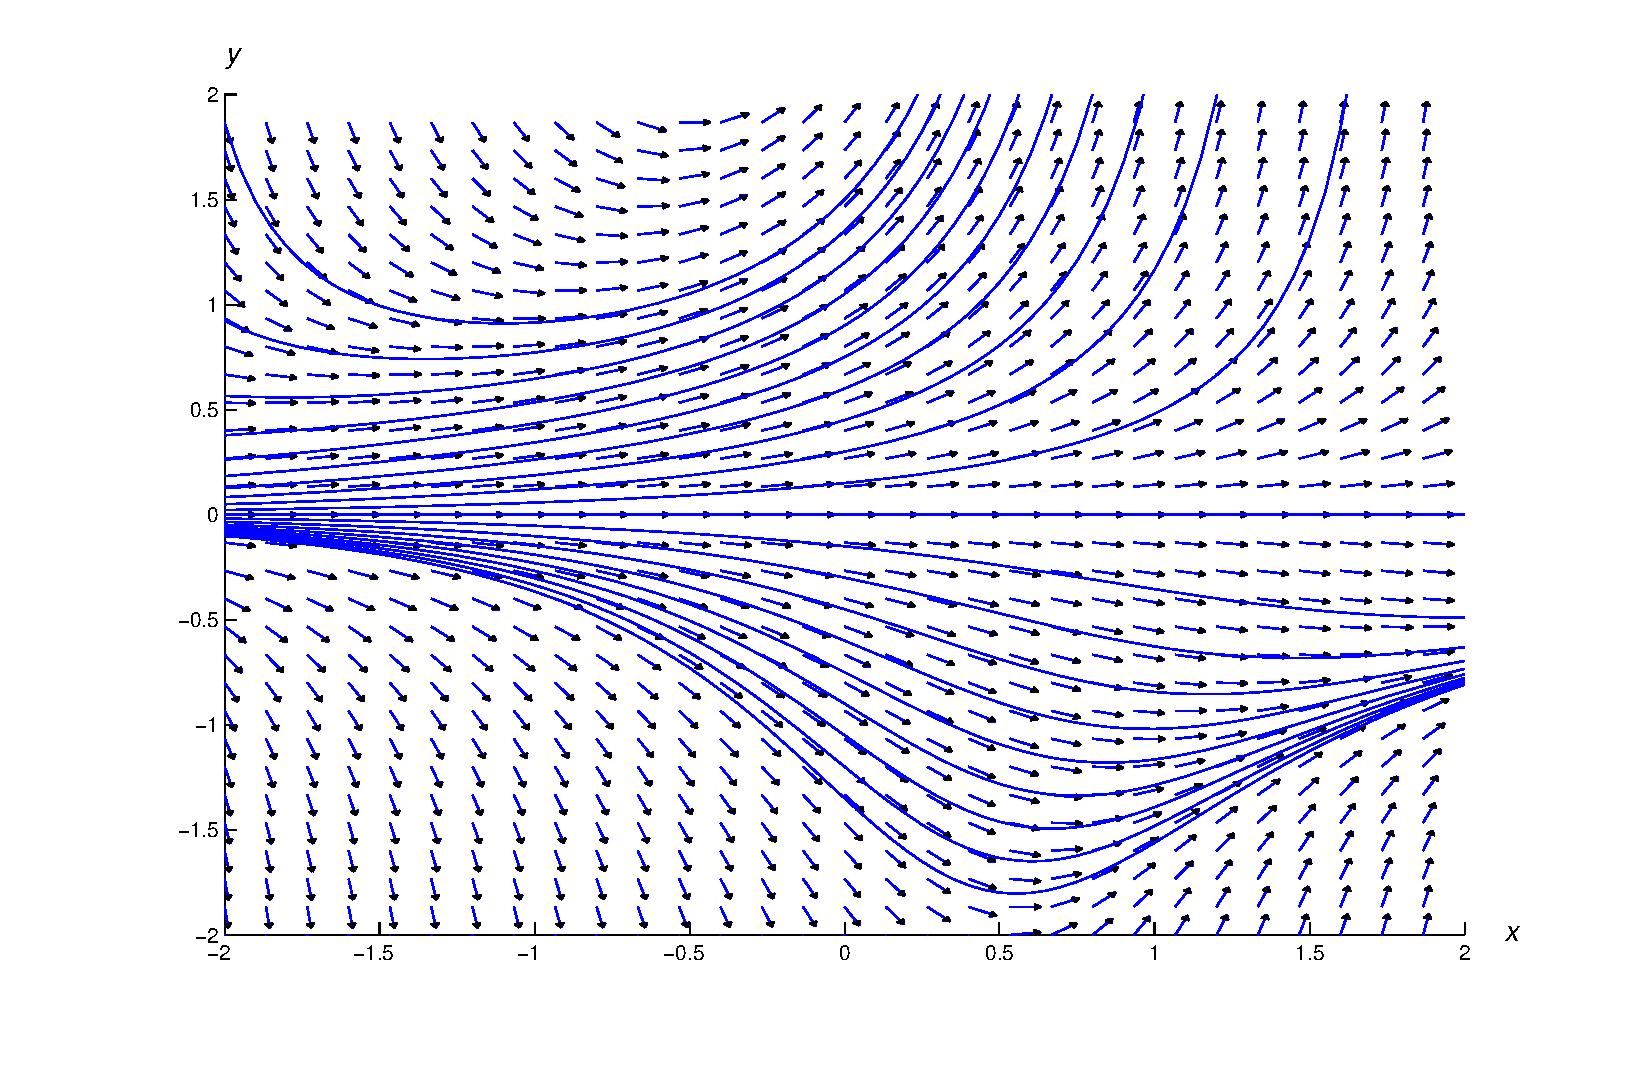
\includegraphics[bb=-78 148 689 643,width=5.67in,height=3.66in,keepaspectratio]{fig020401}
\color{blue}
\caption{A direction field and integral curves for $y'-y=xy^{2}$}
  \label{figure:2.4.1}
\end{figure}


\boxit{Other Nonlinear Equations That Can be  Transformed Into
Separable Equations}

\noindent
We've seen that the nonlinear Bernoulli equation can be transformed
into a separable equation by  the substitution $y=uy_1$ if
$y_1$ is suitably chosen. Now let's discover a sufficient condition
for a nonlinear first order differential equation
\begin{equation} \label{eq:2.4.4}
y'=f(x,y)
\end{equation}
to be transformable into a separable equation in the same way.
  Substituting $y=uy_1$  into
\eqref{eq:2.4.4} yields
$$
u'y_1(x)+uy_1'(x)=f(x,uy_1(x)),
$$
which is equivalent to
\begin{equation} \label{eq:2.4.5}
u'y_1(x)=f(x,uy_1(x))-uy_1'(x).
\end{equation}
If
$$
f(x,uy_1(x))=q(u)y_1'(x)
$$
for some function $q$, then   \eqref{eq:2.4.5} becomes
\begin{equation} \label{eq:2.4.6}
u'y_1(x)=(q(u)-u)y_1'(x),
\end{equation}
which is separable. After checking for constant solutions $u\equiv
u_0$ such that $q(u_0)=u_0$, we can separate
variables to obtain
$$
{u'\over q(u)-u}={y_1'(x)\over y_1(x)}.
$$

\boxit{Homogeneous Nonlinear Equations}


\noindent
In the text  we'll consider only the most widely studied class of
equations for which the method of the preceding paragraph works.
Other types of equations appear in
Exercises~\ref{exer:2.4.44}--\ref{exer:2.4.51}.

The differential equation \eqref{eq:2.4.4}
is said to be {\color{blue}\it homogeneous\/} if  $x$ and $y$
occur in $f$ in such a way that  $f(x,y)$ depends only
on the ratio $y/x$; that is, \eqref{eq:2.4.4} can be written as
\begin{equation} \label{eq:2.4.7}
y'=q(y/x),
\end{equation}
where $q=q(u)$ is a function of a single variable.
For example,
$$
y'={y+xe^{-y/x}\over x}={y\over x}+e^{-y/x}
$$
and
$$
y'={y^2+xy-x^2\over x^2}=\left(y\over x\right)^2+{y\over x}
-1
$$
are of the form  \eqref{eq:2.4.7}, with
$$
q(u)=u+e^{-u}\mbox{\quad and \quad} q(u)=u^2+u-1,
$$
respectively. The general method discussed above can be
applied to
\eqref{eq:2.4.7} with $y_1=x$ (and therefore $y_1'=1)$. Thus,
substituting $y=ux$ in \eqref{eq:2.4.7} yields
$$
u'x+u=q(u),
$$
and separation of variables (after checking for constant
solutions $u\equiv u_0$ such that $q(u_0)=u_0$) yields
$$
{u'\over q(u)-u}={1\over x}.
$$

Before turning to examples, we point out something that you may've have
already noticed:
 the definition of {\color{blue}\it homogeneous equation\/} given
here isn't  the same as the definition given in Section~2.1,
where we said that a linear equation of the form
$$
y'+p(x)y=0
$$
is homogeneous. We make no apology for this inconsistency, since we
didn't create it     historically, {\color{blue}\it homogeneous\/} has been
used in these two inconsistent ways. The one
having to do with linear equations is the most important. This
is the only section of the book where the meaning defined here will
apply.

Since $y/x$ is in general undefined if $x=0$, we'll consider
solutions of nonhomogeneous equations only on open intervals that do
not contain the point $x=0$.

\begin{example}\label{example:2.4.2}\rm
Solve
\begin{equation} \label{eq:2.4.8}
y'={y+xe^{-y/x}\over x}.
\end{equation}
\end{example}

\solution Substituting  $y=ux$
into \eqref{eq:2.4.8} yields
$$
u'x+u =  {ux+xe^{-ux/x}\over x} = u+e^{-u}.
$$
 Simplifying and separating variables yields
$$
e^uu'={1\over x}.
$$
Integrating yields
$e^u=\ln |x|+c$.
Therefore
$u=\ln(\ln|x|+c)$ and
$y=ux=x \ln (\ln |x|+c)$.

Figure~\ref{figure:2.4.2} shows
a direction field and integral curves for \eqref{eq:2.4.8}.


\begin{figure}[H]
  \centering
  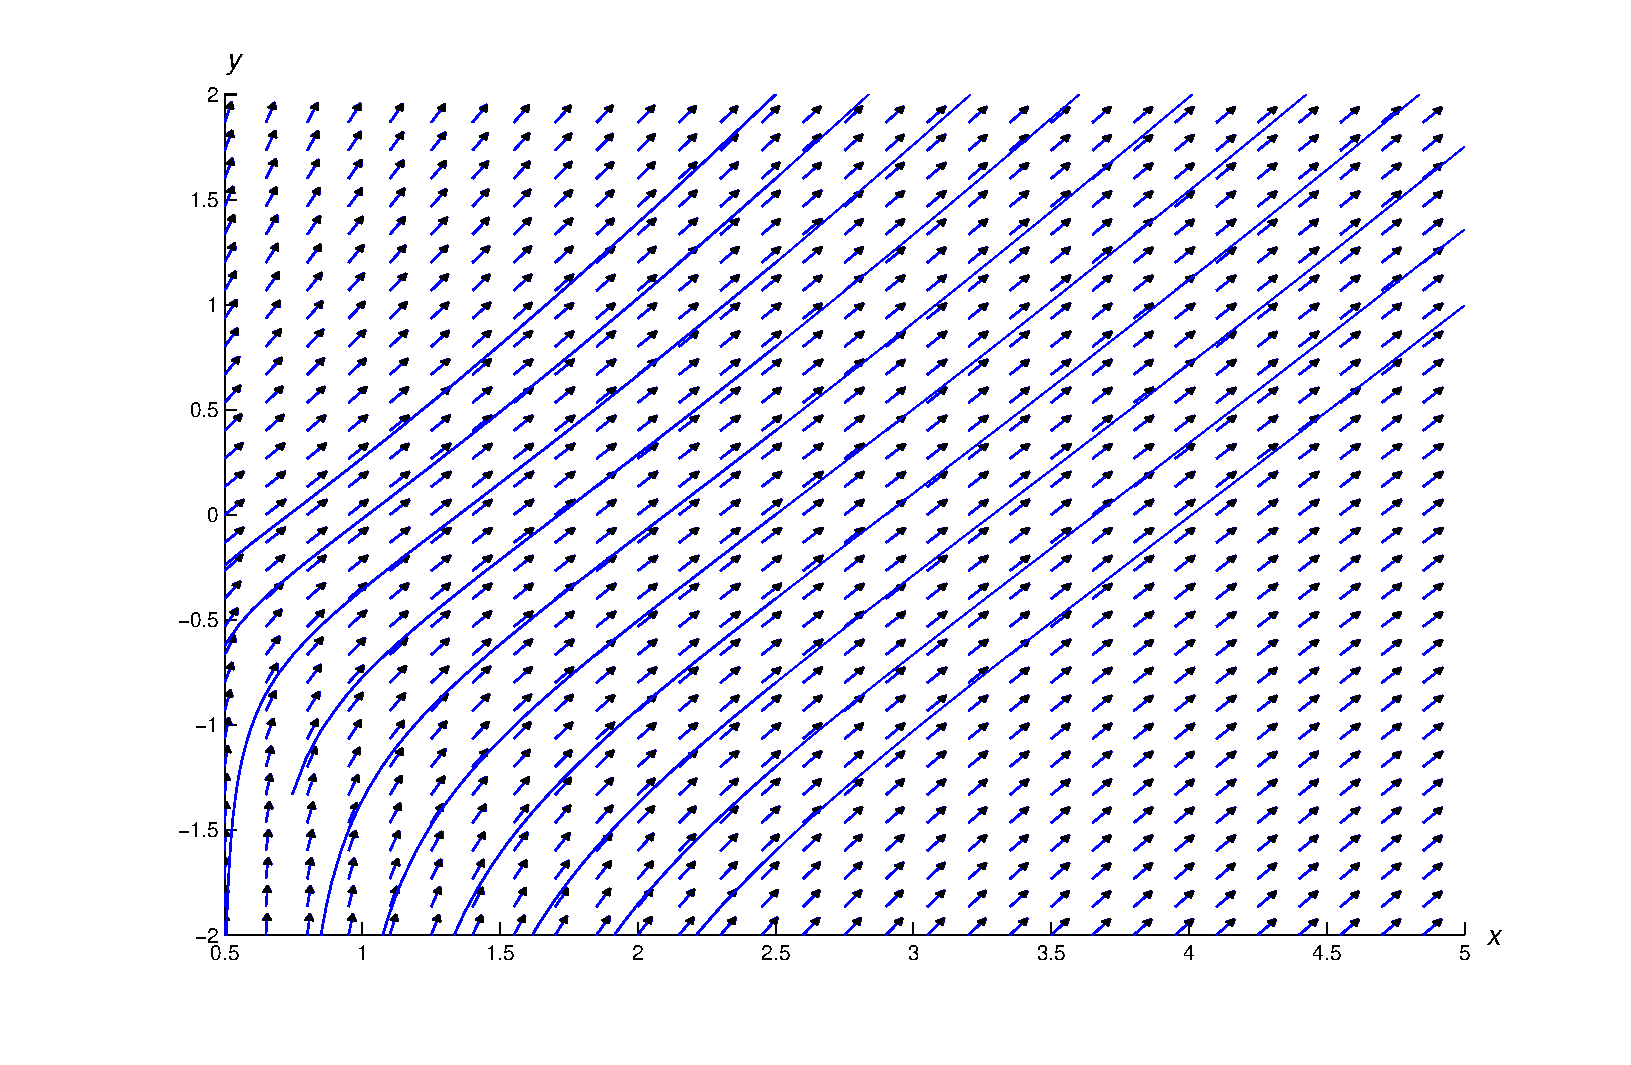
\includegraphics[bb=-78 148 689 643,width=5.67in,height=3.66in,keepaspectratio]{fig020402}
\color{blue}
\caption
{A direction field and some integral curves for
$y'=\dst{\frac{y+xe^{-y/x}}{x}}$}
  \label{figure:2.4.2}
\end{figure}

\begin{example}\label{example:2.4.3}\rm \mbox{}\newline
\begin{alist}
\item %(a)
Solve
\begin{equation} \label{eq:2.4.9}
x^2y'=y^2+xy-x^2.
\end{equation}

\item %(b)
Solve the initial value problem
\begin{equation} \label{eq:2.4.10}
x^2y'=y^2+xy-x^2, \quad y(1)=2.
\end{equation}
\end{alist}
\end{example}

\solutionpart{a}
We first find solutions of \eqref{eq:2.4.9} on open intervals that don't
contain $x=0$. We can rewrite \eqref{eq:2.4.9} as
$$
y'={y^2+xy-x^2\over x^2}
$$
for $x$ in any such interval. Substituting $y=ux$ yields
$$
u'x+u ={ (ux)^2+x(ux)-x^2 \over x^2}
= u^2+u-1,
$$
so
\begin{equation} \label{eq:2.4.11}
u'x=u^2-1.
\end{equation}
By inspection this equation has the constant solutions $u\equiv1$ and
$u\equiv-1$. Therefore $y=x$ and $y=-x$ are solutions of
\eqref{eq:2.4.9}. If $u$ is a solution of \eqref{eq:2.4.11} that doesn't
assume the values $\pm 1$ on some interval,  separating variables
yields
$$
{u'\over u^2-1}={1\over x},
$$
 or, after a partial fraction expansion,
$$
{1\over 2}\left[{1\over u-1}-{1\over u+1}\right]u'=
{1\over x}.
$$
 Multiplying by 2 and integrating yields
$$
\ln\left|u-1\over u+1\right| =2 \ln |x|+k,
$$
 or
$$
\left|{u-1\over u+1}\right|=e^kx^2,
$$
which holds if
\begin{equation} \label{eq:2.4.12}
{u-1\over u+1}=cx^2
\end{equation}
where $c$ is an arbitrary constant.
  Solving for $u$ yields
$$
u ={1+cx^2\over 1-cx^2}.
$$


\begin{figure}[htbp]
\color{blue}
  \begin{minipage}[b]{0.5\linewidth}
    \centering
   \scalebox{.6}{
  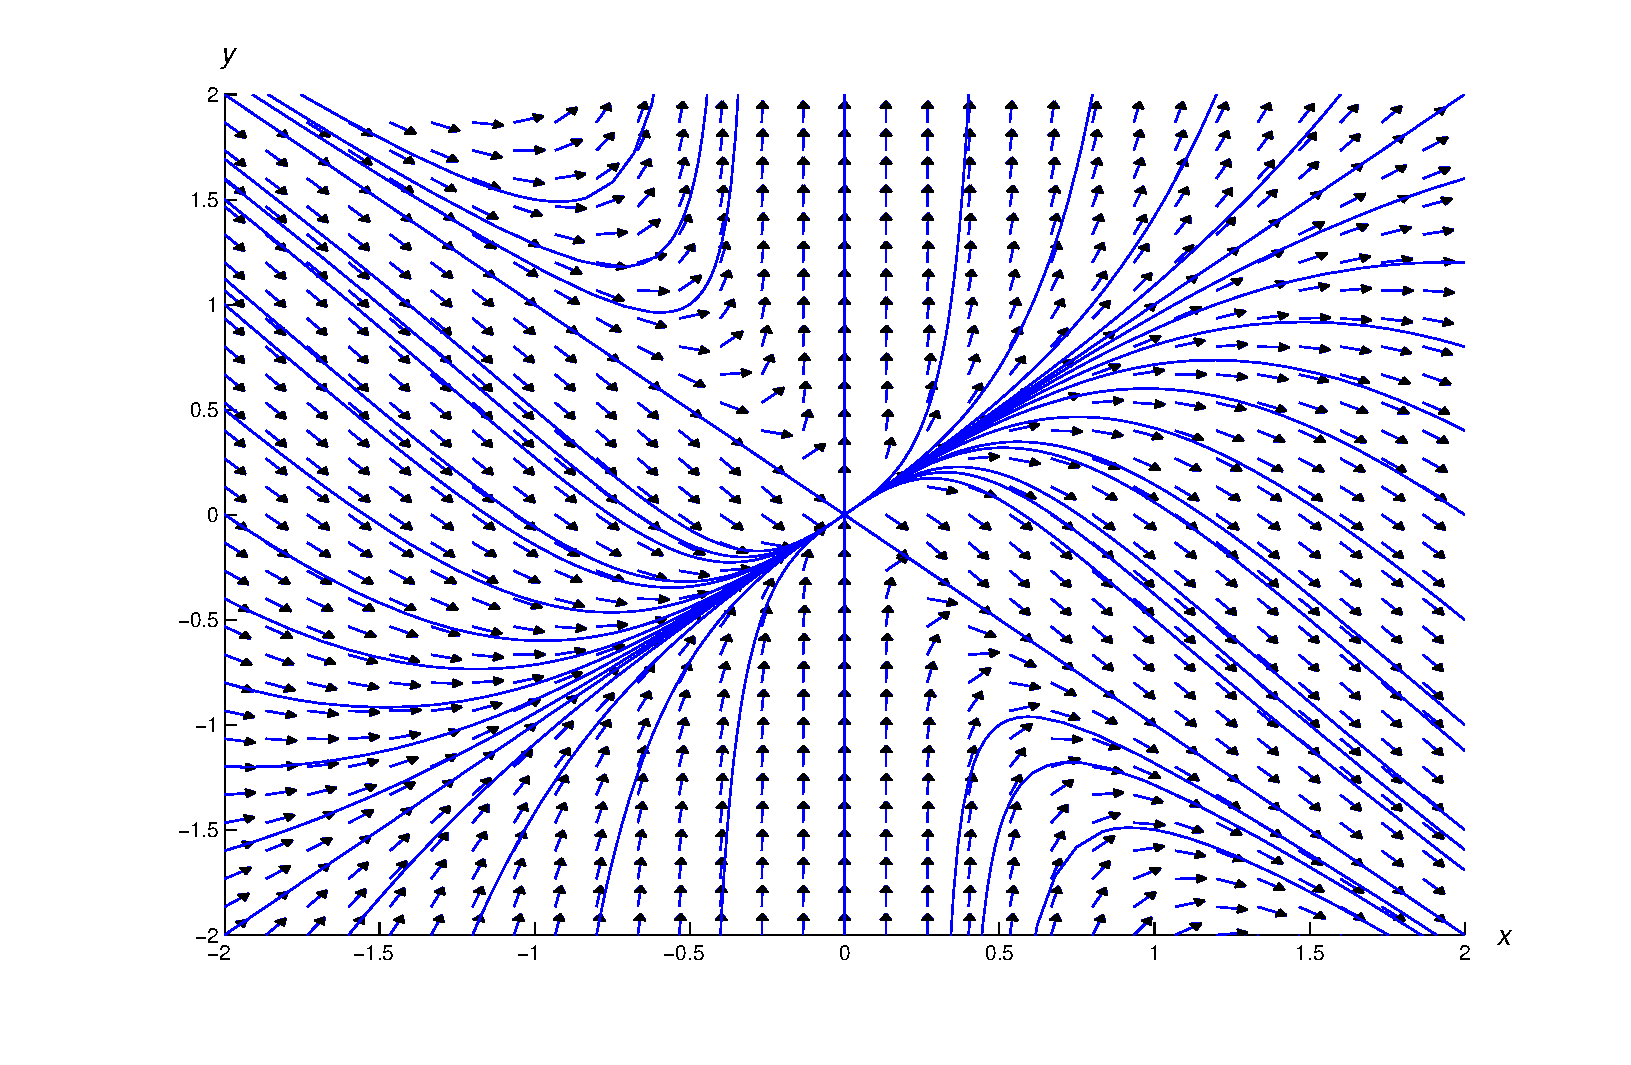
\includegraphics[bb=-78 148 689 643,width=5.67in,height=3.66in,keepaspectratio]{fig020403} }
\color{blue}
\caption{A direction field and  integral curves for
$x^{2}y'=y^{2}+xy-x^{2}$}
  \label{figure:2.4.3}
  \end{minipage}
  \hspace{0.6cm}
  \begin{minipage}[b]{0.5\linewidth}
    \centering
   \scalebox{.7}{
  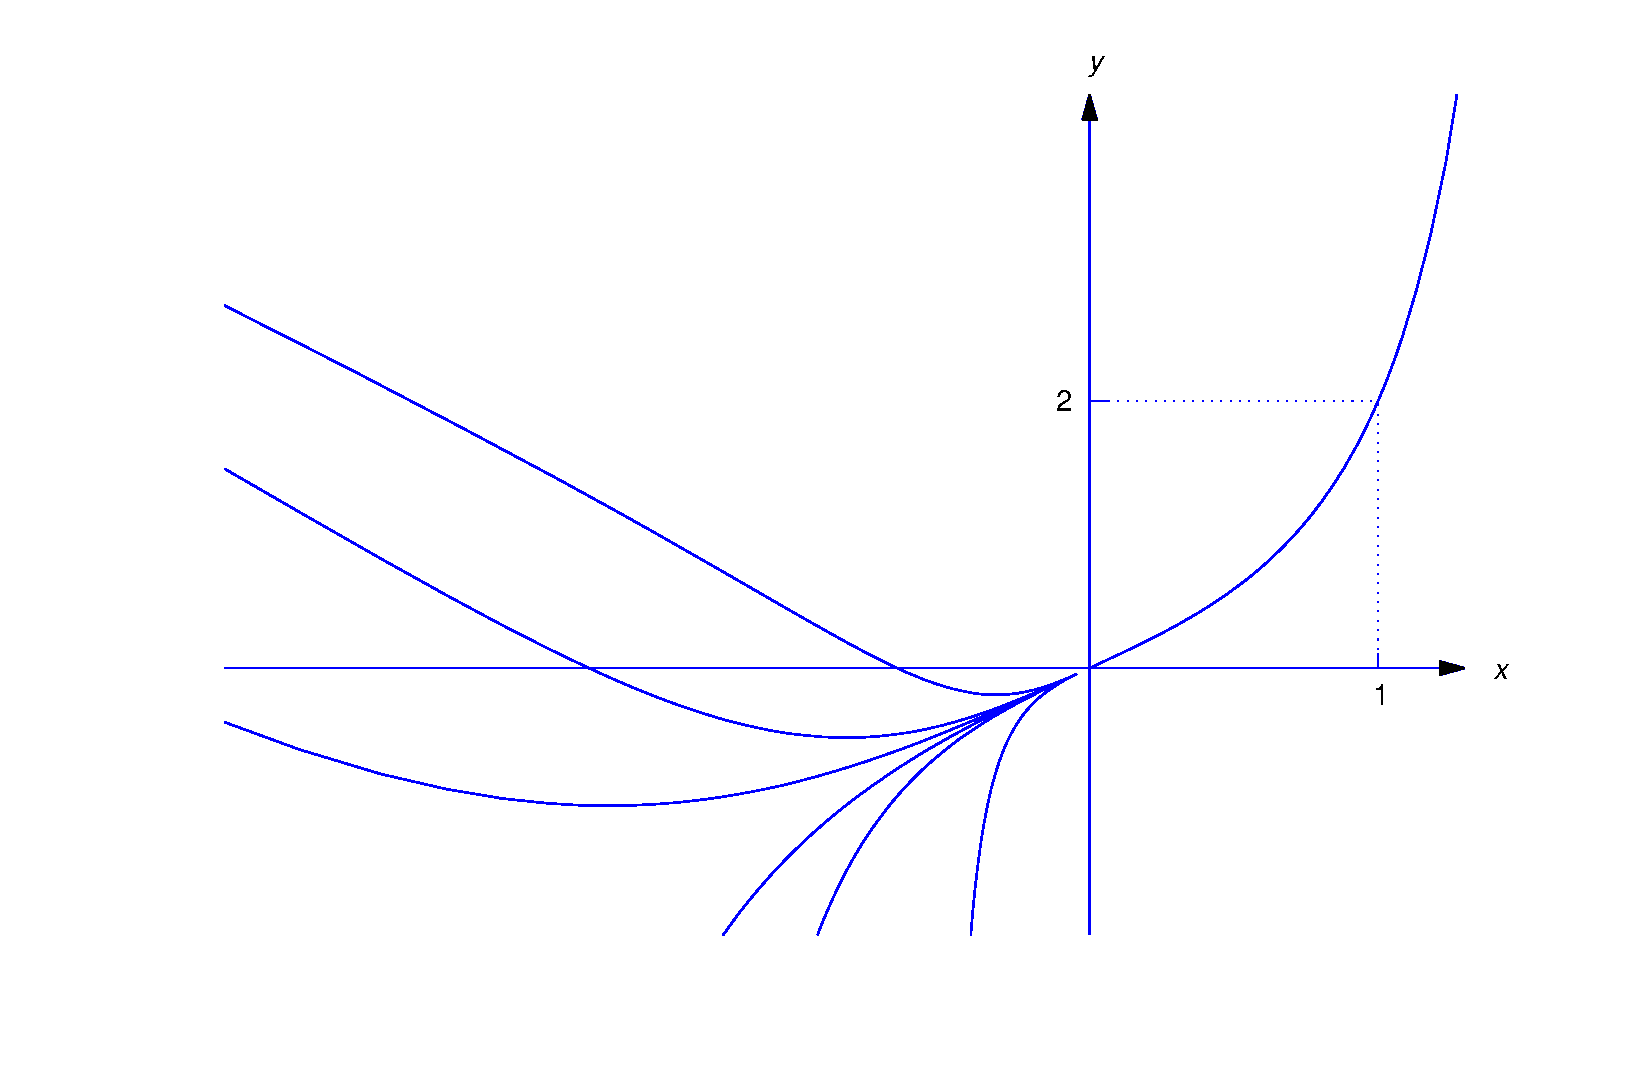
\includegraphics[bb=-78 148 689 643,width=5.67in,height=3.66in,keepaspectratio]{fig020404}}
\caption{Solutions of  $x^{2}y'=y^{2}+xy-x^{2}$,\; $y(1)=2$}
  \label{figure:2.4.4}
  \end{minipage}
\end{figure}





\noindent
Therefore
\begin{equation} \label{eq:2.4.13}
y=ux={x(1+cx^2)\over 1-cx^2}
\end{equation}
is a solution of \eqref{eq:2.4.10} for any choice of the constant $c$.
Setting $c=0$ in \eqref{eq:2.4.13} yields the solution $y=x$. However, the
solution $y=-x$ can't be obtained from \eqref{eq:2.4.13}. Thus, the
solutions of \eqref{eq:2.4.9} on intervals that don't contain $x=0$ are
$y=-x$ and functions of the form \eqref{eq:2.4.13}.

The situation is more complicated if $x=0$ is the open interval.
 First, note that $y=-x$ satisfies \eqref{eq:2.4.9}
on $(-\infty,\infty)$. If $c_1$ and $c_2$ are arbitrary constants,
 the function
\begin{equation} \label{eq:2.4.14}
y=\left\{\begin{array}{ll} \dst{x(1+c_1x^2)\over 1-c_1x^2},&a<x<0,\\
[2\jot]\dst{x(1+c_2x^2)\over 1-c_2x^2},&0\le x<b,
 \end{array}\right.
\end{equation}
is a solution of \eqref{eq:2.4.9} on $(a,b)$, where
$$
a=\left\{\begin{array}{cl}-\dst{1\over\sqrt{c_1}}&\mbox{ if }c_1>0,\\
-\infty&\mbox{ if }c_1\le 0,
\end{array}\right. \mbox{\quad and \quad}
b=\left\{\begin{array}{cl}\dst{1\over\sqrt{c_2}}&\mbox{ if }c_2>0,\\
\infty&\mbox{ if }c_2\le 0.
\end{array}\right.
$$
We leave it to you to verify this. To do so, note that if $y$ is
any function of the form \eqref{eq:2.4.13} then $y(0)=0$ and $y'(0)=1$.


Figure~\ref{figure:2.4.3} shows a direction field and some integral curves
for \eqref{eq:2.4.9}.



\solutionpart{b}  We could obtain $c$ by imposing
the initial condition $y(1)=2$ in \eqref{eq:2.4.13}, and then solving for
$c$. However, it's easier to use \eqref{eq:2.4.12}. Since $u=y/x$, the
initial
condition
$y(1)=2$ implies that $u(1)=2$.  Substituting this into \eqref{eq:2.4.12}
yields $c=1/3$.  Hence, the solution of \eqref{eq:2.4.10} is
$$
y={x(1+x^2/3)\over 1-x^2/3}.
$$
The interval of validity of this solution is $(-\sqrt3,\sqrt3)$.
However, the largest interval on which \eqref{eq:2.4.10} has a unique
solution is $(0,\sqrt3)$. To see this, note from \eqref{eq:2.4.14}
that any function of the form
\begin{equation} \label{eq:2.4.15}
y=\left\{\begin{array}{ll} \dst{x(1+cx^2)\over
1-cx^2},&a<x\le0,\\[2\jot]
\dst{x(1+x^2/3)\over 1-x^2/3},&0\le x<\sqrt3,
\end{array}\right.
\end{equation}
is a solution of \eqref{eq:2.4.10} on $(a,\sqrt3)$, where $a=-1/\sqrt c$
if $c>0$ or $a=-\infty$ if $c\le0$. (Why doesn't this contradict
Theorem~\ref{thmtype:2.3.1}?)


 Figure~\ref{figure:2.4.4} shows several solutions of the
initial value problem~\eqref{eq:2.4.10}. Note that these solutions coincide
on $(0,\sqrt{3})$.

In the last two examples we were able to solve the given equations
explicitly.   However, this isn't  always possible, as you'll
see in the exercises.






\exercises
In Exercises~\ref{exer:2.4.1}--\ref{exer:2.4.4} solve the given Bernoulli
equation.

\begin{exerciselist}

\begin{tabular}[t]{@{}p{168pt}@{}p{168pt}}
\item\label{exer:2.4.1} $y'+y=y^2$ &
\item\label{exer:2.4.2} $\dst {7xy'-2y=-{x^2 \over y^6}}$
\end{tabular}


\begin{tabular}[t]{@{}p{168pt}@{}p{168pt}}
\item\label{exer:2.4.3} $x^2y'+2y=2e^{1/x}y^{1/2}$
& \item\label{exer:2.4.4} \vspace*{-5pt}$\dst {(1+x^2)y'+2xy
={1 \over (1+x^2)y}}$
\end{tabular}

\exercisetext{In Exercises~\ref{exer:2.4.5} and \ref{exer:2.4.6} find all
solutions. Also, plot a direction field and some integral curves on
the indicated rectangular region.}

 \item\label{exer:2.4.5}  \CGex
$y'-xy=x^3y^3;    \quad \{-3\le x\le 3,\-2\le y\ge 2\}$

\item\label{exer:2.4.6} \CGex
$\dst {y'-{1+x\over 3x}y=y^4};   \quad \{-2\le x\le2,-2\le y \le2\}$

\exercisetext{In Exercises~\ref{exer:2.4.7}--\ref{exer:2.4.11} solve the
initial value problem.}

\item\label{exer:2.4.7} $y'-2y=xy^3,\quad y(0)=2\sqrt2$

\item\label{exer:2.4.8} $y'-xy=xy^{3/2},\quad y(1)=4$
\item\label{exer:2.4.9} $xy'+y=x^4y^4,\quad y(1)=1/2$
\item\label{exer:2.4.10} $y'-2y=2y^{1/2},\quad y(0)=1$
\item\label{exer:2.4.11} $\dst{y'-4y={48x\over y^2},\quad y(0)=1}$



\exercisetext{In Exercises~\ref{exer:2.4.12} and \ref{exer:2.4.13} solve the
initial value problem and graph the solution.}

\item\label{exer:2.4.12} \CGex $x^2y'+2xy=y^3,\quad y(1)=1/\sqrt2$
\item\label{exer:2.4.13} \CGex $y'-y=xy^{1/2},\quad y(0)=4$


\item\label{exer:2.4.14}
You may have noticed that  the logistic equation
$$
P'=aP(1-\alpha P)
$$
from Verhulst's model for population growth can be written in
Bernoulli form as
$$
P'-aP=-a\alpha P^2.
$$
This isn't particularly interesting, since the logistic equation is
separable, and therefore solvable by the method studied in
Section~2.2. So let's consider a more complicated model,
where
$a$ is a positive constant and $\alpha$ is a positive continuous
function of $t$ on $[0,\infty)$. The equation for this model is
$$
P'-aP=-a\alpha(t) P^2,
$$
a non-separable Bernoulli equation.
\begin{alist}
\item % (a)
Assuming that $P(0)=P_0>0$, find $P$ for $t>0$. \hint{Express your
result in terms of the integral
 $\int_0^t\alpha(\tau)e^{a\tau}\,d\tau$.}
\item % (b)
Verify that your result reduces to the known results
for the Malthusian model where  $\alpha=0$, and the Verhulst model
where $\alpha$ is a nonzero constant.
\item % (c)
Assuming that
$$
\lim_{t\to\infty}e^{-at}\int_0^t\alpha(\tau)e^{a\tau}\,d\tau=L
$$
exists (finite or infinite), find $\lim_{t\to\infty}P(t)$.
\end{alist}

\exercisetext{In Exercises~\ref{exer:2.4.15}--\ref{exer:2.4.18} solve
the equation explicitly.}

\begin{tabular}[t]{@{}p{168pt}@{}p{168pt}}
 \item\label{exer:2.4.15} $y'=\dst{y+x\over
x}$ & \vspace*{5pt} \item\label{exer:2.4.16}
$y'=\dst{y^2+2xy \over x^2}$
\end{tabular}


\begin{tabular}[t]{@{}p{168pt}@{}p{168pt}}
 \item\label{exer:2.4.17} $xy^3y'=y^4+x^4$ &
 \item\label{exer:2.4.18} $y'=\dst{y\over x}+\sec{y\over x}$
\end{tabular}



\exercisetext{In Exercises~\ref{exer:2.4.19}-\ref{exer:2.4.21} solve the
equation explicitly.
 Also, plot a direction field and some integral curves on
the indicated rectangular region.}

  \item\label{exer:2.4.19} \CGex
$x^2y'=xy+x^2+y^2;   \quad \{-8\le x\le 8,-8\le y\le 8\}$

 \item\label{exer:2.4.20} \CGex
$xyy'=x^2+2y^2;  \quad \{-4\le x\le 4,-4\le y\le 4\}$


\item\label{exer:2.4.21} \CGex
$y'=\dst{2y^2+x^2e^{-(y/x)^2}\over 2xy};
\quad  \{-8\le x\le 8,-8\le y\le 8\}$


\exercisetext{In Exercises~\ref{exer:2.4.22}--\ref{exer:2.4.27} solve
the initial value problem.}

\item\label{exer:2.4.22} $y'=\dst{xy+y^2\over x^2},
\quad y(-1)=2$

 \item\label{exer:2.4.23} $y'=\dst{x^3+y^3\over
xy^2}, \quad y(1)=3$

 \item\label{exer:2.4.24}
 $xyy'+x^2+y^2=0, \quad y(1)=2$

\item\label{exer:2.4.25}
$y'=\dst{y^2-3xy-5x^2 \over x^2}, \quad y(1)=-1$

\item\label{exer:2.4.26}
$x^2y'=2x^2+y^2+4xy, \quad y(1)=1$

\item\label{exer:2.4.27}
$xyy'=3x^2+4y^2, \quad y(1)=\sqrt{3}$

\exercisetext{In Exercises~\ref{exer:2.4.28}--\ref{exer:2.4.34} solve the
given homogeneous equation implicitly.}

\begin{tabular}[t]{@{}p{168pt}@{}p{168pt}}
\item\label{exer:2.4.28} $y'=\dst{x+y \over x-y}$&
\item\label{exer:2.4.29}\vspace*{13pt} $(y'x-y)(\ln |y|-\ln |x|)=x$
\end{tabular}

\begin{tabular}[t]{@{}p{168pt}@{}p{168pt}}
\item\label{exer:2.4.30} $y'=\dst{y^3+2xy^2+x^2y+x^3\over x(y+x)^2}$ &
\item\label{exer:2.4.31}  $y'=\dst{x+2y \over 2x+y}$
\end{tabular}


\begin{tabular}[t]{@{}p{168pt}@{}p{168pt}}
\item\label{exer:2.4.32}  $y'=\dst{y \over y-2x}$&
\item\label{exer:2.4.33} $y'=\dst{xy^2+2y^3\over x^3+x^2y+xy^2}$
\end{tabular}

\item\label{exer:2.4.34} $y'=\dst{x^3+x^2y+3y^3 \over x^3+3xy^2}$


\item\label{exer:2.4.35} \Lex
\begin{alist}
\item % (a)
Find a solution of the initial value problem
$$
x^2y'=y^2+xy-4x^2, \quad y(-1)=0
\eqno{\rm(A)}
$$
on the interval $(-\infty,0)$. Verify that this solution is actually
valid on $(-\infty,\infty)$.
\item % (b)
Use Theorem~\ref{thmtype:2.3.1} to show that (A) has a
unique solution on $(-\infty,0)$.
\item % (c)
Plot a direction field for the differential equation in
(A) on a square
$$
\{-r\le x\le r, -r\le y\le r\},
$$
where $r$
is any positive number. Graph the solution you obtained in
\part{a} on this field.
\item % (d)
Graph  other solutions  of (A) that are defined on $(-\infty,\infty)$.
\item % (e)
Graph other solutions of (A)  that are defined only on intervals of
the form $(-\infty,a)$, where is a finite positive number.
\end{alist}



\item\label{exer:2.4.36} \Lex
\begin{alist}
\item % (a)
Solve the equation
$$
xyy'=x^2-xy+y^2
\eqno{\rm(A)}
$$
implicitly.
\item % (b)
Plot a direction field for (A) on a square
$$
\{0\le x\le r,0\le y\le r\}
$$
where $r$ is any positive number.
\item % (c)
Let $K$ be a positive integer. (You may have to try several
choices for $K$.)
Graph solutions of the initial value problems
$$
xyy'=x^2-xy+y^2,\quad y(r/2)={kr\over K},
$$
for $k=1$, $2$, \dots, $K$. Based on your observations, find
 conditions on the positive numbers $x_0$
and $y_0$ such that the initial value problem
$$
xyy'=x^2-xy+y^2,\quad y(x_0)=y_0,
\eqno{\rm(B)}
$$
has  a unique solution (i) on $(0,\infty)$   or (ii) only
on an interval  $(a,\infty)$, where $a>0$?
\item % (d)
What can you say about the graph of the solution of (B)
as $x\to\infty$? (Again, assume that $x_0>0$ and $y_0>0$.)
\end{alist}


\item\label{exer:2.4.37} \Lex
\begin{alist}
\item % (a)
Solve the equation
$$
y'={2y^2-xy+2x^2 \over xy+2x^2}
\eqno{\rm(A)}
$$
implicitly.
\item % (b)
Plot a direction field for (A) on a square
$$
\{-r\le x\le r,-r\le y\le r\}
$$
where $r$ is any positive number. By graphing solutions of (A),
determine necessary and sufficient conditions on $(x_0,y_0)$ such that
(A) has a solution on (i) $(-\infty,0)$ or (ii) $(0,\infty)$ such that
$y(x_0)=y_0$.
\end{alist}

\item\label{exer:2.4.38} \Lex
Follow the instructions of Exercise~\ref{exer:2.4.37} for the equation
$$
y'={xy+x^2+y^2 \over xy}.
$$

\item\label{exer:2.4.39} \Lex
Pick any  nonlinear homogeneous equation $y'=q(y/x)$  you like, and
plot  direction fields on the square $\{-r\le x\le r,\ -r\le y\le
r\}$,
where $r>0$. What happens to the direction field as you vary $r$?
Why?

\item\label{exer:2.4.40}
Prove:  If $ad-bc\ne 0$, the equation
$$
y'={ax+by+\alpha \over cx+dy+\beta}
$$
can be transformed into the homogeneous nonlinear equation
$$
{dY \over dX}={aX+bY \over cX+dY}
$$
by the substitution $x=X-X_0,\  y=Y-Y_0$,
where $X_0$ and $Y_0$ are suitably chosen constants.

\exercisetext{In Exercises~\ref{exer:2.4.41}-\ref{exer:2.4.43} use a
method suggested by Exercise~\ref{exer:2.4.40} to solve the
given equation implicitly.}

\begin{tabular}[t]{@{}p{168pt}@{}p{168pt}}
\item\label{exer:2.4.41} $y'=\dst{-6x+y-3 \over 2x-y-1}$
& \item\label{exer:2.4.42}\vspace*{10pt} $y'=\dst{2x+y+1 \over x+2y-4}$
\end{tabular}

\item\label{exer:2.4.43}
$y'=\dst{-x+3y-14 \over x+y-2}$

\exercisetext{In Exercises~\ref{exer:2.4.44}--\ref{exer:2.4.51} find
a function $y_1$ such that the substitution $y=uy_1$ transforms
the given equation  into a separable
equation of the form \eqref{eq:2.4.6}. Then solve the given equation
explicitly.}

\begin{tabular}[t]{@{}p{168pt}@{}p{168pt}}
\item\label{exer:2.4.44} $3xy^2y'=y^3+x$ & \vspace*{10pt}
\item\label{exer:2.4.45} $xyy'=3x^6+6y^2$
\end{tabular}

\begin{tabular}[t]{@{}p{168pt}@{}p{168pt}}
\item\label{exer:2.4.46} $x^3y'=2(y^2+x^2y-x^4)$ &
\item\label{exer:2.4.47} $y'=y^2e^{-x}+4y+2e^x$
\end{tabular}

\begin{tabular}[t]{@{}p{168pt}@{}p{168pt}}
\item\label{exer:2.4.48} $y'=\dst{y^2+y\tan x+\tan^2 x\over\sin^2x}$ &
\item\label{exer:2.4.49} $x(\ln x)^2y'=-4(\ln x)^2+y\ln x+y^2$
\end{tabular}

\begin{tabular}[t]{@{}p{168pt}@{}p{168pt}}
\item\label{exer:2.4.50} $2x(y+2\sqrt x)y'=(y+\sqrt x)^2$&
\item\label{exer:2.4.51} $(y+e^{x^2})y'=2x(y^2+ye^{x^2}+e^{2x^2})$
\end{tabular}

\medskip
\item\label{exer:2.4.52}
Solve the initial value problem
$$
y'+{2\over x}y={3x^2y^2+6xy+2\over x^2(2xy+3)},\quad y(2)=2.
$$

\item\label{exer:2.4.53}
Solve the initial value problem
$$
y'+{3\over x}y={3x^4y^2+10x^2y+6\over x^3(2x^2y+5)},\quad y(1)=1.
$$

\item\label{exer:2.4.54}
 Prove:  If $y$ is a solution of a homogeneous nonlinear equation
$y'=q(y/x)$,  so is $y_1=y(ax)/a$, where $a$ is any nonzero
constant.


\item\label{exer:2.4.55}
A {\color{blue}\it generalized}
\href{http://http://www-history.mcs.st-and.ac.uk/Indexes/Riccati.html}
{\color{blue}\it Riccati equation} is of the form
$$
y'=P(x)+Q(x)y+R(x)y^2.
\eqno{\rm (A)}
$$
(If $R\equiv-1$,  (A) is a
\href{http://http://www-history.mcs.st-and.ac.uk/Indexes/Riccati.html}
{\color{blue}\it Riccati
equation\/}.) Let $y_1$ be a known solution and $y$ an arbitrary
solution of (A). Let $z=y-y_1$. Show that $z$ is a
solution of a Bernoulli equation with $n=2$.


\exercisetext{In Exercises~\ref{exer:2.4.56}--\ref{exer:2.4.59},
given that $y_1$ is a solution of the given equation, use the
method suggested by Exercise \ref{exer:2.4.55} to find other solutions.}

\item\label{exer:2.4.56} $y'=1+x - (1+2x)y+xy^2$;  \quad    $y_1=1$

\item\label{exer:2.4.57} $y'=e^{2x}+(1-2e^x)y+y^2$;  \quad    $y_1=e^x$

\item\label{exer:2.4.58} $xy'=2-x+(2x-2)y-xy^2$;  \quad    $y_1=1$

\item\label{exer:2.4.59} $xy'=x^3+(1-2x^2)y+xy^2$;  \quad    $y_1=x$

\end{exerciselist}


\newsection{5}{First Order Equations} {Exact Equations}
\currentpdfbookmark{Section 2.5 Exact Equations}{section:2.5}
\vskip14pt
\renewcommand{\thissection}{\sectiontitle{\,
EXACT EQUATIONS}}
\thissection


\noindent
In this  section it's convenient to write first order
differential equations in the form
\begin{equation} \label{eq:2.5.1}
M(x,y)\,dx+N(x,y)\,dy=0.
\end{equation}
This equation  can be interpreted as
\begin{equation} \label{eq:2.5.2}
M(x,y)+N(x,y)\,{dy\over dx}=0,
\end{equation}
where $x$ is the independent variable and $y$ is the dependent
variable, or as
\begin{equation} \label{eq:2.5.3}
M(x,y)\,{dx\over dy}+N(x,y)=0,
\end{equation}
where $y$ is the independent variable and $x$ is the dependent
variable. Since the solutions of \eqref{eq:2.5.2} and \eqref{eq:2.5.3} will
often have to be left in
implicit, form we'll say that $F(x,y)=c$ is an implicit solution of
\eqref{eq:2.5.1} if every differentiable function $y=y(x)$ that satisfies
$F(x,y)=c$ is a solution of \eqref{eq:2.5.2} and every
differentiable function $x=x(y)$ that satisfies $F(x,y)=c$ is a
solution of \eqref{eq:2.5.3}.

Here are  some examples:

\begin{center}\label{table:2.5.1}\vspace*{6pt}

\begin{tabular}{|c|c|c|} \hline
& & \\[-6pt]
Equation \eqref{eq:2.5.1}&Equation \eqref{eq:2.5.2}&Equation \eqref{eq:2.5.3}
\\[9pt]\hline & & \\[-6pt]
$3x^2y^2\,dx+2x^3y\,dy =0$ &$3x^2y^2+2x^3y\,\dst{dy\over
dx} =0$  &$3x^2y^2\,\dst{dx\over dy}+2x^3y=0$
\\[9pt]\hline
& & \\[-6pt]
$(x^2+y^2)\,dx +2xy\,dy=0$ &
$(x^2+y^2)+2xy\,\dst{dy\over dx}=0$&
$(x^2+y^2)\,\dst{dx\over dy} +2xy=0$
\\[9pt]\hline
& & \\[-6pt]
$3y\sin x\,dx-2xy\cos x\,dy =0$
&$3y\sin x-2xy\cos x\,\dst{dy\over dx} =0$
& $3y\sin x\,\dst{dx\over dy}-2xy\cos x  =0$
\\[9pt]\hline
\end{tabular}
\end{center}

Note that a separable equation can be written as
\eqref{eq:2.5.1} as
$$
M(x)\,dx+N(y)\,dy=0.
$$


We'll  develop a method for solving \eqref{eq:2.5.1} under appropriate
assumptions on $M$ and $N$. This method is an extension
of the method of separation of variables
(Exercise~\ref{exer:2.5.41}).  Before stating it we
consider an  example.

\begin{example}\label{example:2.5.1} \rm
Show that
\begin{equation} \label{eq:2.5.4}
x^4y^3+x^2y^5+2xy=c
\end{equation}
is an implicit solution of
\begin{equation} \label{eq:2.5.5}
(4x^3y^3+2xy^5+2y)\,dx+(3x^4y^2+5x^2y^4+2x)\,dy=0.
\end{equation}
\end{example}

\solution
Regarding $y$ as a function of $x$ and
differentiating \eqref{eq:2.5.4} implicitly with respect to
$x$ yields
$$
(4x^3y^3+2xy^5+2y)+(3x^4y^2+5x^2y^4+2x)\,{dy\over dx}=0.
$$
Similarly, regarding $x$ as a function of $y$ and
differentiating \eqref{eq:2.5.4} implicitly with respect to
$y$ yields
$$
(4x^3y^3+2xy^5+2y){dx\over dy}+(3x^4y^2+5x^2y^4+2x)=0.
$$
Therefore \eqref{eq:2.5.4} is an implicit solution of \eqref{eq:2.5.5}
in either of its two possible interpretations. \bbox

You may think this example is pointless, since
concocting a differential equation that has a given implicit solution
isn't particularly interesting. However, it illustrates the
next important theorem, which  we'll prove by using implicit
differentiation,  as  in  Example~\ref{example:2.5.1}.

\begin{theorem}\color{blue} \label{thmtype:2.5.1}
If $F=F(x,y)$ has continuous partial derivatives
$F_x$ and $F_y$, then
\begin{equation} \label{eq:2.5.6}
F(x,y)=c\qquad \mbox{{\rm(}$c$=constant\mbox{)}},
\end{equation}
is an implicit solution of the differential equation
\begin{equation} \label{eq:2.5.7}
F_x(x,y)\,dx+F_y(x,y)\,dy=0.
\end{equation}
\end{theorem}

\proof Regarding $y$ as a function of $x$ and  differentiating
\eqref{eq:2.5.6}  implicitly with respect to $x$ yields
$$
F_x(x,y)+F_y(x,y)\,{dy\over dx}=0.
$$
On the other hand,
 regarding $x$ as a function of $y$ and  differentiating
\eqref{eq:2.5.6}  implicitly with respect to $y$ yields
$$
F_x(x,y)\,{dx\over dy}+F_y(x,y)=0.
$$
Thus, \eqref{eq:2.5.6} is an
implicit solution of  \eqref{eq:2.5.7} in either of its two possible
interpretations. \bbox

We'll say that  the equation
\begin{equation} \label{eq:2.5.8}
M(x,y)\,dx+N(x,y)\,dy=0
\end{equation}
 is  {\color{blue}\it exact} on an an open rectangle  $R$ if there's
a function $F=F(x,y)$ such  $F_x$
and $F_y$  are continuous, and
\begin{equation} \label{eq:2.5.9}
F_x(x,y)=M(x,y) \mbox{\quad and \quad} F_y(x,y)=N(x,y)
\end{equation}
for  all  $(x,y)$ in $R$.
This usage of ``exact'' is related  to its usage in calculus,
where the expression
$$
F_x(x,y)\,dx+F_y(x,y)\,dy
$$
(obtained by substituting \eqref{eq:2.5.9} into the left side of
\eqref{eq:2.5.8}) is the  {\color{blue}\it exact differential of\/} $F$.

Example~\ref{example:2.5.1} shows that it's easy to solve
\eqref{eq:2.5.8}
if it's exact {\color{blue}\it and}  we know a function $F$ that satisfies
\eqref{eq:2.5.9}. The important questions are:

 {\sc Question 1.}  Given an equation
\eqref{eq:2.5.8}, how can we determine whether it's  exact?

 {\sc Question 2.} If \eqref{eq:2.5.8} is exact, how do we find
a function $F$ satisfying \eqref{eq:2.5.9}?

To discover the answer to Question~1,
 assume that  there's a function $F$  that satisfies \eqref{eq:2.5.9} on
some open rectangle $R$, and in addition that $F$ has continuous mixed
partial derivatives $F_{xy}$ and $F_{yx}$.  Then a theorem from calculus
implies that
\begin{equation} \label{eq:2.5.10}
F_{xy}=F_{yx}.
\end{equation}
If $F_x=M$ and $F_y=N$,
differentiating the first of these equations with respect to
$y$ and the second with respect to $x$ yields
\begin{equation} \label{eq:2.5.11}
F_{xy}=M_y\mbox{\quad and \quad}  F_{yx}=N_x.
\end{equation}
From  \eqref{eq:2.5.10}  and \eqref{eq:2.5.11}, we conclude that
 a necessary condition for exactness is that $M_y=N_x$.
This motivates the next theorem, which we state without proof.

\begin{theorem}\color{blue} $[$The Exactness
Condition$]$\label{thmtype:2.5.2}
 \space  Suppose  $M$ and
$N$ are continuous and have continuous partial derivatives
$M_y$ and $N_x$ on an open rectangle $R.$ Then
$$
M(x,y)\,dx+N(x,y)\,dy=0
$$
is exact on $R$ if and only if
\begin{equation} \label{eq:2.5.12}
M_y(x,y)=N_x(x,y)
\end{equation}
for all $(x,y)$ in  $R.$.
\end{theorem}

To help you  remember the exactness condition, observe
that the coefficients of $dx$ and $dy$ are differentiated in
\eqref{eq:2.5.12} with respect to the ``opposite'' variables; that is,
the coefficient of $dx$ is differentiated with respect to $y$, while the
coefficient of $dy$ is differentiated with respect to $x$.

\begin{example}\label{example:2.5.2} \rm
 Show that the equation
$$
3x^2y\,dx+4x^3\,dy=0
$$
is not exact on any open rectangle.
\end{example}

\solution   Here
$$
M(x,y)=3x^2y\mbox{\quad and \quad} N(x,y)=4x^3
$$
so
$$
M_y(x,y)=3x^2 \mbox{\quad and \quad} N_x(x,y)=12 x^2.
$$
Therefore  $M_y=N_x$   on the line $x=0$,
but not on any open rectangle, so
there's no
function $F$ such that $F_x(x,y)=M(x,y)$ and $F_y(x,y)=N(x,y)$
for all $(x,y)$ on any open rectangle.
\bbox

The next example illustrates two possible methods for finding a
function $F$ that satisfies the condition $F_x=M$ and $F_y=N$ if
$M\,dx+N\,dy=0 $ is exact.

\begin{example}\label{example:2.5.3} \rm
Solve
\begin{equation} \label{eq:2.5.13}
(4x^3y^3+3x^2)\,dx+(3x^4y^2+6y^2)\,dy=0.
\end{equation}
\end{example}


\solution{(Method 1)}
Here
$$
M(x,y)=4x^3y^3+3x^2,\quad N(x,y)=3x^4y^2+6y^2,
$$
and
$$
M_y(x,y)=N_x(x,y)=12 x^3y^2
$$
for all $(x,y)$.
Therefore
Theorem~\ref{thmtype:2.5.2} implies that there's a function $F$ such that
\begin{equation} \label{eq:2.5.14}
F_x(x,y)=M(x,y)=4x^3y^3+3x^2
\end{equation}
 and
\begin{equation} \label{eq:2.5.15}
F_y(x,y)=N(x,y)=3x^4y^2+6y^2
\end{equation}
 for all $(x,y)$.  To find $F$, we integrate \eqref{eq:2.5.14} with
respect to $x$ to obtain
\begin{equation} \label{eq:2.5.16}
F(x,y)=x^4y^3+x^3+\phi(y),
\end{equation}
 where $\phi (y)$ is the ``constant'' of integration.  (Here
$\phi$ is ``constant'' in  that it's independent of $x$, the
variable of integration.)  If $\phi$ is any differentiable function of
$y$ then $F$  satisfies \eqref{eq:2.5.14}.  To
determine $\phi$ so that
$F$ also satisfies \eqref{eq:2.5.15}, assume that $\phi$ is
differentiable and differentiate $F$ with respect to $y$.
This yields
$$
F_y(x,y)=3x^4y^2+\phi'(y).
$$
 Comparing this with \eqref{eq:2.5.15} shows that
$$
\phi'(y)=6y^2.
$$
 We integrate this with respect to $y$ and take the
constant of integration to be zero because we're interested only in
finding {\color{blue}\it some} $F$ that satisfies \eqref{eq:2.5.14} and
\eqref{eq:2.5.15}. This  yields
$$
\phi (y)=2y^3.
$$
Substituting this into \eqref{eq:2.5.16} yields
\begin{equation} \label{eq:2.5.17}
F(x,y)=x^4y^3+x^3+2y^3.
\end{equation}
Now Theorem~\ref{thmtype:2.5.1} implies that
$$
x^4y^3+x^3+2y^3=c
$$
is an implicit solution of \eqref{eq:2.5.13}. Solving this for $y$
yields the explicit solution
$$
y=\left(c-x^3\over2+x^4\right)^{1/3}.
$$

\solution{(Method 2)} Instead of first integrating
\eqref{eq:2.5.14}
with respect to $x$, we could begin by integrating \eqref{eq:2.5.15} with
respect to $y$ to obtain
\begin{equation} \label{eq:2.5.18}
F(x,y)=x^4y^3+2y^3+\psi (x),
\end{equation}
 where $\psi$ is an arbitrary  function of
$x$.  To determine $\psi$, we assume that $\psi$ is
differentiable and differentiate $F$ with respect to $x$,
which yields
$$
F_x(x,y)=4x^3y^3+\psi'(x).
$$
 Comparing this with \eqref{eq:2.5.14} shows that
$$
\psi'(x)=3x^2.
$$
Integrating this and again taking  the constant of
integration to be zero yields
$$
\psi(x)=x^3.
$$
 Substituting this into \eqref{eq:2.5.18} yields \eqref{eq:2.5.17}.

Figure~\ref{figure:2.5.1} shows a direction field and  some
integral curves of \eqref{eq:2.5.13},

              \begin{figure}[tbp]
  \centering
  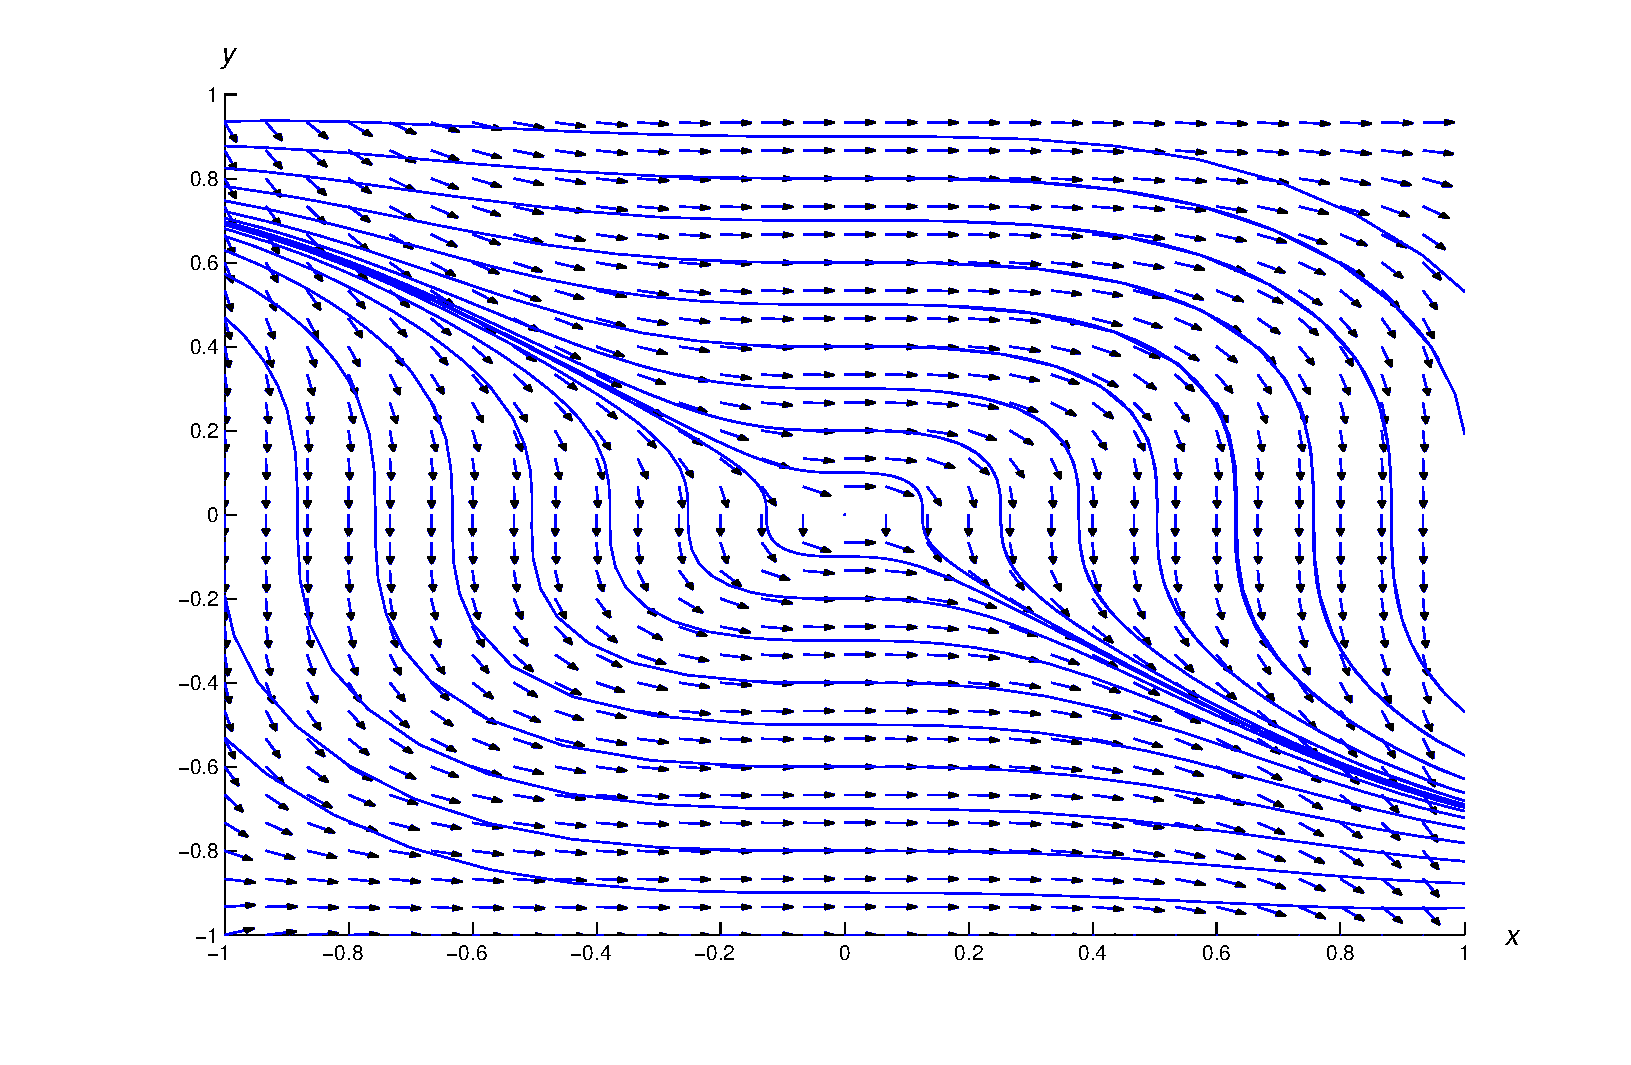
\includegraphics[bb=-78 148 689 643,width=5.67in,height=3.66in,keepaspectratio]{fig020501}
\color{blue}
\caption{A direction field and  integral curves for
$(4x^3y^3+3x^2)\,dx+(3x^4y^2+6y^2)\,dy=0$}
  \label{figure:2.5.1}
\end{figure}



Here's a summary of the procedure used in Method 1 of this
example. You should summarize procedure used in Method~2.

\smallskip
\color{blue}
{\centerline{{\bf Procedure For Solving An Exact
Equation}}


\begin{description}
\item{\bf Step 1.} Check that the equation
\begin{equation} \label{eq:2.5.19}
 M(x,y)\,dx+N(x,y)\,dy=0
\end{equation}
satisfies the exactness condition  $M_y=N_x$. If not,
don't go further with this procedure.
\item{\bf Step 2.} Integrate
$$
{\partial F(x,y)\over\partial x}=M(x,y)
$$
with respect to $x$ to obtain
\begin{equation} \label{eq:2.5.20}
F(x,y)=G(x,y)+\phi(y),
\end{equation}
where $G$ is an antiderivative of $M$ with respect to $x$, and $\phi$
is an unknown function of $y$.
\item{\bf Step 3.} Differentiate \eqref{eq:2.5.20} with respect to
$y$  to obtain
$$
{\partial F(x,y)\over\partial y}={\partial G(x,y)\over\partial
y}+\phi'(y).
$$
\item{\bf Step 4.} Equate the right side of this equation to $N$ and solve
for $\phi'$;    thus,
$$
 {\partial G(x,y)\over\partial y}+\phi'(y)=N(x,y),\mbox{\quad  so \quad }
\phi'(y)=N(x,y)-{\partial G(x,y)\over\partial y}.
$$
\item{\bf Step 5.} Integrate $\phi'$ with respect to $y$, taking the
constant of integration to be zero, and substitute the result in
\eqref{eq:2.5.20} to obtain $F(x,y)$.
\item{\bf Step 6.} Set $F(x,y)=c$ to obtain an implicit solution of
\eqref{eq:2.5.19}. If possible, solve for $y$ explicitly as a
function of $x$.
\end{description}
\color{black}


It's a common mistake to omit Step 6. However, it's important to
include this step, since $F$ isn't  itself a solution of
\eqref{eq:2.5.19}.

Many equations can be conveniently solved by either of the two methods
used in Example~\ref{example:2.5.3}. However, sometimes the integration
required in one approach is  more difficult than in the
other. In such cases we choose the approach that requires the easier
integration.

\begin{example}\label{example:2.5.4} \rm
 Solve the equation
\begin{equation}  \label{eq:2.5.21}
(ye^{xy} \tan x+e^{xy} \sec^2x)\,dx+xe^{xy} \tan x\,dy=0.
\end{equation}
\end{example}

\solution We leave it to you to check that
$M_y=N_x$ on any open rectangle  where $\tan x$ and $\sec x$ are
defined. Here we must find a function $F$ such that
\begin{equation} \label{eq:2.5.22}
F_x(x,y)=ye^{xy} \tan x+e^{xy} \sec^2 x
\end{equation}
 and
\begin{equation}  \label{eq:2.5.23}
F_y(x,y)=xe^{xy} \tan x.
\end{equation}
 It's difficult to integrate \eqref{eq:2.5.22} with respect to $x$, but
easy to integrate \eqref{eq:2.5.23} with respect to $y$.  This yields
\begin{equation} \label{eq:2.5.24}
F(x,y)=e^{xy} \tan x+\psi (x).
\end{equation}
Differentiating this with respect to $x$ yields
$$
F_x(x,y)=ye^{xy}\tan x+e^{xy}\sec^2x+\psi'(x).
$$
 Comparing this with \eqref{eq:2.5.22} shows that  $\psi'(x)=0$.
Hence, $\psi$ is  a constant, which we can take to be zero in
\eqref{eq:2.5.24}, and
$$
e^{xy} \tan x=c
$$
is an implicit solution of \eqref{eq:2.5.21}. \bbox

Attempting to apply our procedure to an equation that isn't  exact
will lead to failure in  Step 4, since the function
$$
 N-{\partial G\over\partial y}
$$
won't be independent of $x$ if $M_y\ne N_x$
(Exercise~\ref{exer:2.5.31}), and therefore
can't be the derivative of a function of $y$ alone. Here's an example that
illustrates this.

\begin{example}\label{example:2.5.5}  \rm
 Verify that the equation
\begin{equation} \label{eq:2.5.25}
3x^2y^2\,dx+6x^3y\,dy=0
\end{equation}
is not exact, and show  that the procedure for solving exact equations
  fails when applied to \eqref{eq:2.5.25}.
\end{example}

\solution   Here
$$
M_y(x,y)=6x^2y \mbox{\quad  and \quad } N_x(x,y)=18x^2y,
$$
so \eqref{eq:2.5.25} isn't  exact. Nevertheless,  let's try to find
a function $F$ such that
\begin{equation} \label{eq:2.5.26}
F_x(x,y)=3x^2y^2
\end{equation}
and
\begin{equation} \label{eq:2.5.27}
F_y(x,y)=6x^3y.
\end{equation}
Integrating \eqref{eq:2.5.26} with respect to $x$ yields
$$
F(x,y)=x^3y^2+\phi(y),
$$
and differentiating this with respect to $y$ yields
$$
F_y(x,y)=2x^3y+\phi'(y).
$$
For this equation to be consistent with \eqref{eq:2.5.27},
$$
6x^3y=2x^3y+\phi'(y),
$$
or
$$
\phi'(y)=4x^3y.
$$
This is a contradiction, since $\phi'$  must be independent
of $x$. Therefore the procedure fails.

\exercises
In Exercises~\ref{exer:2.5.1}--\ref{exer:2.5.17} determine which equations
are exact and solve them.

\begin{exerciselist}
\item\label{exer:2.5.1}
$6x^2y^2\,dx+4x^3y\,dy=0$

\item\label{exer:2.5.2}
$(3y\cos x+4xe^x+2x^2e^x)\,dx+(3\sin x+3)\,dy=0$

\item\label{exer:2.5.3}
$14x^2y^3\,dx+21 x^2y^2\,dy=0$

\item\label{exer:2.5.4}
$(2x-2y^2)\,dx+(12y^2-4xy)\,dy=0$

\begin{tabular}[t]{@{}p{168pt}@{}p{168pt}}
 \item\label{exer:2.5.5}$(x+y)^2\,dx+(x+y)^2\,dy=0$&
\item\label{exer:2.5.6}$(4x+7y)\,dx+(3x+4y)\,dy=0$
\end{tabular}

\item\label{exer:2.5.7}
$(-2y^2\sin x+3y^3-2x)\,dx+(4y\cos x+9xy^2)\,dy=0$

\item\label{exer:2.5.8}
$(2x+y)\,dx+(2y+2x)\,dy=0$

\item\label{exer:2.5.9}
$(3x^2+2xy+4y^2)\,dx+(x^2+8xy+18y)\,dy=0$

\item\label{exer:2.5.10}
$(2x^2+8xy+y^2)\,dx+(2x^2+xy^3/3)\,dy=0$

\item\label{exer:2.5.11}
$\dst{\left({1\over x}+2x\right)\,dx+
\left({1\over y}+2y\right)\,dy=0}$

\item\label{exer:2.5.12}
$(y\sin xy+xy^2\cos xy)\,dx+(x\sin xy+xy^2\cos xy)\,dy=0$

\item\label{exer:2.5.13}
$\dst{{x\,dx\over(x^2+y^2)^{3/2}}+{y\,dy
\over(x^2+y^2)^{3/2}}=0}$

\item\label{exer:2.5.14}
$\left(e^x(x^2y^2+2xy^2)+6x\right)\,dx+(2x^2ye^x+2)\,dy=0$

\item\label{exer:2.5.15}
$\left(x^2e^{x^2+y}(2x^2+3)+4x\right)\,dx+(x^3e^{x^2+y}-12y^2)\,dy=0$

\item\label{exer:2.5.16}
$\left(e^{xy}(x^4y+4x^3)+3y\right)\,dx+(x^5e^{xy}+3x)\,dy=0$

\item\label{exer:2.5.17}
$(3x^2\cos xy-x^3y\sin xy+4x)\,dx+(8y-x^4\sin xy)\,dy=0$

\exercisetext{In Exercises~\ref{exer:2.5.18}--\ref{exer:2.5.22} solve
the initial value problem.}

\item\label{exer:2.5.18}
$(4x^3y^2-6x^2y-2x-3)\,dx+(2x^4y-2x^3)\,dy=0,\quad y(1)=3$

\item\label{exer:2.5.19}
$(-4y\cos x+4\sin x\cos x+\sec^2x)\,dx+
(4y-4\sin x)\,dy=0,\quad y(\pi/4)=0$

\item\label{exer:2.5.20}
$(y^3-1)e^x\,dx+3y^2(e^x+1)\,dy=0,\quad y(0)=0$

\item\label{exer:2.5.21}
$(\sin x-y\sin x-2\cos x)\,dx+\cos x\,dy=0,\quad y(0)=1$

\item\label{exer:2.5.22}
$(2x-1)(y-1)\,dx+(x+2)(x-3)\,dy=0,\quad y(1)=-1$

\item\label{exer:2.5.23} \CGex
Solve the exact equation
$$
(7x+4y)\,dx+(4x+3y)\,dy=0.
$$
Plot a direction field and some integral curves for this equation on
the rectangle
$$
\{-1\le x\le1,-1\le y\le1\}.
$$

\item\label{exer:2.5.24} \CGex
Solve the exact equation
$$
e^x(x^4y^2+4x^3y^2+1)\,dx+(2x^4ye^x+2y)\,dy=0.
$$
Plot a direction field and some integral curves for this equation on
the rectangle
$$
\{-2\le x\le2,-1\le y\le1\}.
$$

\item\label{exer:2.5.25} \CGex
Plot a direction field and some integral curves for the exact equation
$$
(x^3y^4+x)\,dx+(x^4y^3+y)\,dy=0
$$
on the rectangle $\{-1\le x\le 1,-1\le y\le1\}$. (See
Exercise~\ref{exer:2.5.37}\part{a}).

\item\label{exer:2.5.26} \CGex
Plot a direction field and some integral curves for the exact equation
$$
(3x^2+2y)\,dx+(2y+2x)\,dy=0
$$
on the rectangle $\{-2\le x\le 2,-2\le y\le2\}$. (See
Exercise~\ref{exer:2.5.37}(b)).

\item\label{exer:2.5.27} \Lex
\begin{alist}
\item % (a)
Solve the exact equation
$$
(x^3y^4+2x)\,dx+(x^4y^3+3y)\,dy=0
\eqno{\rm(A)}
$$
implicitly.
\item % (b)
For what choices of $(x_0,y_0)$ does
Theorem~\ref{thmtype:2.3.1} imply that the initial value problem
$$
(x^3y^4+2x)\,dx+(x^4y^3+3y)\,dy=0,\quad y(x_0)=y_0,
\eqno{\rm(B)}
$$
has a unique solution on an open interval $(a,b)$  that contains $x_0$?
\item % (b)
Plot a direction field and some integral curves for (A)
on a rectangular region centered at the origin. What is the
 interval of validity of the solution of (B)?
\end{alist}

\item\label{exer:2.5.28} \Lex
\begin{alist}
\item % (a)
Solve the exact equation
$$
(x^2+y^2)\,dx+2xy\,dy=0
\eqno{\rm(A)}
$$
implicitly.
\item % (b)
For what choices of $(x_0,y_0)$ does
Theorem~\ref{thmtype:2.3.1} imply that the initial value problem
$$
(x^2+y^2)\,dx+2xy\,dy=0,\quad y(x_0)=y_0,
\eqno{\rm(B)}
$$
has a unique solution $y=y(x)$ on some open interval $(a,b)$
that contains $x_0$?
\item % (c)
Plot a direction field and some integral curves for (A). From
the plot determine,
the  interval $(a,b)$ of \part{b}, the monotonicity
properties (if any) of the solution of (B), and $\lim_{x\to
a+}y(x)$ and $\lim_{x\to b-}y(x)$. \hint{Your answers will
depend upon which quadrant contains $(x_0,y_0)$.}
\end{alist}

\item\label{exer:2.5.29}
Find all functions $M$ such that the  equation is exact.
\begin{alist}
\item %(a)
$M(x,y)\,dx+(x^2-y^2)\,dy=0$
\item %(b)
$M(x,y)\,dx+2xy\sin x\cos y\,dy=0$
\item %(c)
$M(x,y)\,dx+(e^x-e^y\sin x)\,dy=0$
\end{alist}

\item\label{exer:2.5.30}
Find all functions $N$ such that the  equation is exact.
\begin{alist}
\item %(a)
$(x^3y^2+2xy+3y^2)\,dx+N(x,y)\,dy=0$
\item %(b)
$(\ln xy+2y\sin x)\,dx+N(x,y)\,dy=0$
\item %(c)
$(x\sin x+y\sin y)\,dx+N(x,y)\,dy=0$
\end{alist}

\item\label{exer:2.5.31}
Suppose $M,N,$ and their partial derivatives are continuous on
an open rectangle
$R$, and $G$ is an antiderivative of $M$ with respect to $x$; that is,
$$
{\partial G\over\partial x}=M.
$$
Show that if $M_y\ne N_x$ in $R$ then the function
$$
 N-{\partial  G\over\partial y}
$$
is not independent of $x$.

\item\label{exer:2.5.32}
Prove:  If the equations $M_1\,dx+N_1\,dy=0$ and $M_2\,
dx+N_2\,dy=0$ are exact on an open rectangle $R$,  so is
the equation $$(M_1+M_2)\,dx+(N_1+N_2)\,dy=0.$$

\item\label{exer:2.5.33}
Find conditions on the constants $A$, $B$, $C$, and $D$ such that
the equation
$$
(Ax+By)\,dx+(Cx+Dy)\,dy=0
$$
is exact.

\item\label{exer:2.5.34}
Find conditions on the constants $A$, $B$, $C$, $D$, $E$, and
$F$ such that the equation
$$
(Ax^2+Bxy+Cy^2)\,dx+(Dx^2+Exy+Fy^2)\,dy=0
$$
is exact.

\item\label{exer:2.5.35}
Suppose $M$ and $N$ are continuous and have continuous partial
derivatives $M_y$ and $N_x$ that satisfy the exactness condition
$M_y=N_x$ on an open rectangle $R$.
  Show that if $(x,y)$ is in $R$ and
$$
F(x,y)=\int^x_{x_0}M(s,y_0)\,ds+\int^y_{y_0}N(x,t)\,dt,
$$
then $F_x=M$ and $F_y=N$.

\item\label{exer:2.5.36}
Under the assumptions of Exercise~\ref{exer:2.5.35}, show that
$$
F(x,y)=\int^y_{y_0}N(x_0,s)\,ds+\int^x_{x_0}M(t,y)\,dt.
$$

\item\label{exer:2.5.37}
Use the method suggested by Exercise~\ref{exer:2.5.35}, with
$(x_0,y_0)=(0,0)$, to solve the these exact equations:
\begin{alist}
\item %(a)
$(x^3y^4+x)\,dx+(x^4y^3+y)\,dy=0$
\item %(b)
$(x^2+y^2)\,dx+2xy\,dy=0$
\item %(c)
$(3x^2+2y)\,dx+(2y+2x)\,dy=0$
\end{alist}

\item\label{exer:2.5.38}
Solve the initial value problem
$$
y'+{2\over x}y=-{2xy\over x^2+2x^2y+1},\quad y(1)=-2.
$$

\item\label{exer:2.5.39}
Solve the initial value problem
$$
y'-{3\over x}y={2x^4(4x^3-3y)\over3x^5+3x^3+2y},\quad y(1)=1.
$$

\item\label{exer:2.5.40}
Solve the initial value problem
$$
y'+2xy=-e^{-x^2}\left({3x+2ye^{x^2}\over2x+3ye^{x^2}}\right),\quad
y(0)=-1.
$$

\item\label{exer:2.5.41}
Rewrite the separable equation
$$
h(y)y'=g(x)
\eqno{\rm (A)}
$$
as an exact equation
$$
M(x,y)\,dx+N(x,y)\,dy=0.
\eqno{\rm (B)}
$$
Show that applying the method of this section  to
(B) yields the same solutions that would be
obtained by applying the method of separation of variables
to~(A)

\item\label{exer:2.5.42}
Suppose  all second partial derivatives of $M=M(x,y)$ and $N=N(x,y)$
are continuous and $M\,dx+N\,dy=0$ and $-N\,dx+M\,dy=0$ are
exact on an open rectangle  $R$.  Show that
$M_{xx}+M_{yy}=N_{xx}+N_{yy}=0$ on
$R$.

\item\label{exer:2.5.43} Suppose all second partial derivatives of
$F=F(x,y)$ are continuous and $F_{xx}+F_{yy}=0$ on an open rectangle
$R$. (A function with these properties is said to be {\color{blue}\it harmonic\/};
see also Exercise~\ref{exer:2.5.42}.) Show that $-F_y\,dx+F_x\,dy=0$ is
exact on $R$, and
therefore there's a function $G$ such that
$G_x=-F_y$ and $G_y=F_x$ in $R$. (A function $G$ with this property is
said to be a {\color{blue}\it harmonic conjugate\/} of $F$.)

\item\label{exer:2.5.44}
Verify that the following functions are harmonic, and find all their
harmonic conjugates.  (See Exercise~\ref{exer:2.5.43}.)

\begin{tabular}[t]{@{}p{112pt}@{}p{112pt}p{112pt}}
{\bf (a)}\   $x^2-y^2$
& {\bf (b)}\   $e^x\cos y$
& {\bf (c)}\   $x^3-3xy^2$\\
{\bf (d)}\   $\cos x\cosh y$
& {\bf (e)}\   $\sin x\cosh y$ &
\end{tabular}

\end{exerciselist}


\newsection{6}{Integrating Factors} {Exact Equations}
\currentpdfbookmark{Section 2.6 Exact Equations}{section:2.6}
\vskip14pt
\renewcommand{\thissection}{\sectiontitle{\,
INTEGRATING FACTORS}}
\thissection


\noindent
In  Section~2.5 we saw that if $M$, $N$, $M_y$ and $N_x$ are
continuous and $M_y=N_x$ on an open rectangle $R$ then
\begin{equation} \label{eq:2.6.1}
M(x,y)\,dx+N(x,y)\,dy=0
\end{equation}
is exact on $R$. Sometimes an equation that isn't  exact can be made
exact by multiplying it by an appropriate function. For example,
\begin{equation}\label{eq:2.6.2}
(3x+2y^2)\,dx+2xy\,dy=0
\end{equation}
is  not exact, since
$M_y(x,y)=4y\ne  N_x(x,y)=2y$ in \eqref{eq:2.6.2}.
 However, multiplying \eqref{eq:2.6.2}  by $x$ yields
\begin{equation}\label{eq:2.6.3}
(3x^2+2xy^2)\,dx+2x^2y\,dy=0,
\end{equation}
which is exact, since
$M_y(x,y)=N_x(x,y)=4xy$ in \eqref{eq:2.6.3}.
Solving \eqref{eq:2.6.3} by the procedure given in  Section~2.5
 yields the implicit solution
$$
x^3+x^2y^2=c.
$$

A function $\mu=\mu(x,y)$ is  an {\color{blue}\it integrating factor} for
\eqref{eq:2.6.1}  if
\begin{equation}\label{eq:2.6.4}
 \mu(x,y)M (x,y)\,dx+\mu(x,y)N (x,y)\,dy=0
 \end{equation}
 is exact. If we know an integrating
factor $\mu$ for \eqref{eq:2.6.1}, we can solve the exact equation
\eqref{eq:2.6.4} by the method of Section~2.5. It would be
nice
if we could say that \eqref{eq:2.6.1} and \eqref{eq:2.6.4} always have the
same solutions, but this isn't so. For example, a solution
$y=y(x)$ of \eqref{eq:2.6.4} such that $\mu(x,y(x))=0$ on some interval
$a<x<b$ could fail to be a solution of \eqref{eq:2.6.1}
(Exercise~\ref{exer:2.6.1}), while
\eqref{eq:2.6.1} may have a solution $y=y(x)$ such that $\mu(x,y(x)) $
isn't even defined (Exercise~\ref{exer:2.6.2}). Similar comments
apply if $y$ is the independent variable and $x$ is the dependent
variable  in \eqref{eq:2.6.1} and \eqref{eq:2.6.4}.  However, if $\mu(x,y)$
is defined and nonzero for all $(x,y)$,  \eqref{eq:2.6.1}  and
\eqref{eq:2.6.4} are equivalent; that is, they have the same solutions.

\boxit{Finding Integrating Factors}


\noindent
By applying Theorem~\ref{thmtype:2.5.2} (with $M$ and $N$ replaced by $\mu M$
and $\mu N$), we see that \eqref{eq:2.6.4} is exact on an open rectangle
$R$ if $\mu M$, $\mu N$, $(\mu M)_y$, and $(\mu N)_x$ are continuous
and
$$
{\partial\over\partial y}(\mu M)={\partial\over\partial x}
(\mu N) \mbox{\quad or, equivalently, \quad}
\mu_yM+\mu M_y=\mu_xN+\mu N_x
$$
on $R$. It's better to rewrite the last equation as
\begin{equation} \label{eq:2.6.5}
\mu(M_y-N_x)=\mu_xN-\mu_yM,
\end{equation}
which  reduces to  the known result for exact equations;
that is, if $M_y=N_x$ then \eqref{eq:2.6.5} holds with $\mu=1$, so
\eqref{eq:2.6.1} is exact.

You may think  \eqref{eq:2.6.5} is of little value, since it involves
{\color{blue}\it partial\/} derivatives of the unknown integrating factor $\mu$,
and we haven't studied methods for solving such equations. However,
we'll now show that \eqref{eq:2.6.5} is useful if we restrict our search
to integrating factors that are products of a function of
$x$ and a function of $y$; that is,
$\mu(x,y)=P(x)Q(y)$.
We're not saying that {\color{blue}\it every\/} equation
 $M\,dx+N\,dy=0$ has an integrating factor of this
form;   rather, we're saying that {\color{blue}\it some\/} equations have
such integrating
factors.We'llnow develop a way to determine whether a given
equation has such an integrating factor, and a method for finding the
integrating factor in this case.


If $\mu(x,y)=P(x)Q(y)$, then $\mu_x(x,y)=P'(x)Q(y)$ and
$\mu_y(x,y)=P(x)Q'(y)$, so \eqref{eq:2.6.5} becomes
\begin{equation} \label{eq:2.6.6}
P(x)Q(y)(M_y-N_x)=P'(x)Q(y)N-P(x)Q'(y)M,
\end{equation}
or, after dividing through by $P(x)Q(y)$,
\begin{equation} \label{eq:2.6.7}
M_y-N_x={P'(x)\over P(x)}N-{Q'(y)\over Q(y)}M.
\end{equation}
Now let
$$
p(x)={P'(x)\over P(x)} \mbox{\quad and \quad} q(y)={Q'(y)\over Q(y)},
$$
so \eqref{eq:2.6.7} becomes
\begin{equation} \label{eq:2.6.8}
M_y-N_x=p(x)N-q(y)M.
\end{equation}

We obtained \eqref{eq:2.6.8} by {\color{blue}\it assuming\/} that $M\,dx+N\,dy=0$ has
an integrating factor $\mu(x,y)=P(x)Q(y)$. However, we can
now view \eqref{eq:2.6.7} differently: If there are functions $p=p(x)$
and $q=q(y)$  that satisfy \eqref{eq:2.6.8} and we define
\begin{equation} \label{eq:2.6.9}
P(x)=\pm e^{\int p(x)\,dx}\mbox{\quad and \quad}
Q(y)=\pm e^{\int q(y)\,dy},
\end{equation}
then reversing the steps that led from \eqref{eq:2.6.6} to
\eqref{eq:2.6.8} shows that $\mu(x,y)=P(x)Q(y)$ is an integrating factor
for $M\,dx+N\,dy=0$. In using this result, we take the constants of
integration in \eqref{eq:2.6.9} to be zero and choose the signs
conveniently so the integrating factor has the simplest form.

There's no simple general method for ascertaining
whether functions $p=p(x)$ and $q=q(y)$ satisfying \eqref{eq:2.6.8}
exist. However, the next theorem gives simple sufficient
conditions for the given equation to have an integrating factor that
depends on only one of the independent variables $x$ and $y$, and for
finding an integrating factor in this case.

\begin{theorem}\color{blue}\label{thmtype:2.6.1}
Let $M,$ $N,$ $M_y,$ and $N_x$ be continuous on an open rectangle $R.$
Then$:$
\begin{alist}
\item % (a)
 If $(M_y-N_x)/N$ is independent
of $y$ on $R$ and  we define
$$
p(x)={M_y-N_x\over N}
$$
 then
\begin{equation}\label{eq:2.6.10}
\mu(x)=\pm e^{\int p(x)\,dx}
\end{equation}
is an integrating factor for
\begin{equation}\label{eq:2.6.11}
M(x,y)\,dx+N(x,y)\,dy=0
\end{equation}
on $R.$
\item % (b)
If $(N_x-M_y)/M$ is independent of $x$ on
$R$ and we define
$$
q(y)={N_x-M_y\over M},
$$
then
\begin{equation}\label{eq:2.6.12}
\mu(y)=\pm e^{\int q(y)\,dy}
\end{equation}
 is an integrating factor for \eqref{eq:2.6.11} on $R.$
\end{alist}
\end{theorem}

\medskip

\proof (a)
If $(M_y-N_x)/N$ is independent of $y$, then \eqref{eq:2.6.8}
 holds with $p=(M_y-N_x)/N$ and $q\equiv0$. Therefore
 $$
P(x)=\pm e^{\int p(x)\,dx}\mbox{\quad and\quad}Q(y)=\pm e^{\int
q(y)\,dy}=\pm e^0=\pm1,
 $$
so \eqref{eq:2.6.10} is an integrating factor for \eqref{eq:2.6.11} on $R$.

(b) If $(N_x-M_y)/M$ is independent of $x$ then eqref{eq:2.6.8} holds
with $p\equiv0$ and $q=(N_x-M_y)/M$, and a similar argument shows that
\eqref{eq:2.6.12} is an integrating factor for \eqref{eq:2.6.11} on $R$.\bbox

The next two examples show how to apply
Theorem~\ref{thmtype:2.6.1}.

\begin{example}\label{example:2.6.1}
\rm  Find an integrating factor for the equation
\begin{equation}\label{eq:2.6.13}
(2xy^3-2x^3y^3-4xy^2+2x)\,dx+(3x^2y^2+4y)\,dy=0
\end{equation}
and solve the equation.
\end{example}

\solution In \eqref{eq:2.6.13}
$$
M=2xy^3-2x^3y^3-4xy^2+2x,\ N=3x^2y^2+4y,
$$
and
$$
M_y-N_x=(6xy^2-6x^3y^2-8xy)-6xy^2=-6x^3y^2-8xy,
$$
so \eqref{eq:2.6.13}  isn't  exact. However,
$$
{M_y-N_x\over N}=-{6x^3y^2+8xy\over
3x^2y^2+4y}=-2x
$$
is independent of $y$, so Theorem~\ref{thmtype:2.6.1}\part{a} applies
with
$p(x)=-2x$. Since
$$
\int p (x)\,dx=-\int 2x\,dx=-x^2,
$$
 $\mu(x)=e^{-x^2}$ is an
integrating factor.  Multiplying \eqref{eq:2.6.13} by $\mu$ yields the
exact equation
\begin{equation}\label{eq:2.6.14}
e^{-x^2}(2xy^3-2x^3y^3-4xy^2+2x)\,dx+
 e^{-x^2}(3x^2y^2+4y)\,dy=0.
\end{equation}

To solve this equation, we must find a
function $F$ such that
\begin{equation}\label{eq:2.6.15}
F_x(x,y)=e^{-x^2}(2xy^3-2x^3y^3-4xy^2+2x)
\end{equation}
 and
\begin{equation}\label{eq:2.6.16}
F_y(x,y)=e^{-x^2}(3x^2y^2+4y).
\end{equation}
 Integrating \eqref{eq:2.6.16} with respect to $y$ yields
\begin{equation}\label{eq:2.6.17}
F(x,y)=e^{-x^2}(x^2y^3+2y^2)+\psi(x).
\end{equation}
 Differentiating this with respect to $x$ yields
$$
F_x(x,y)=e^{-x^2}(2xy^3-2x^3y^3-4xy^2)+\psi'(x).
$$
Comparing this with \eqref{eq:2.6.15} shows that $\psi'(x)=
2xe^{-x^2}$;  therefore, we can let $\psi(x)=-e^{-x^2}$ in
\eqref{eq:2.6.17} and conclude that
$$
e^{-x^2}\left(y^2(x^2y+2)-1\right)=c
$$
is an implicit solution of \eqref{eq:2.6.14}. It is also an implicit solution
of \eqref{eq:2.6.13}.

Figure~\ref{figure:2.6.1}  shows a  direction field and some integal curves
for \eqref{eq:2.6.13}

  \begin{figure}[tbp]
  \centering
  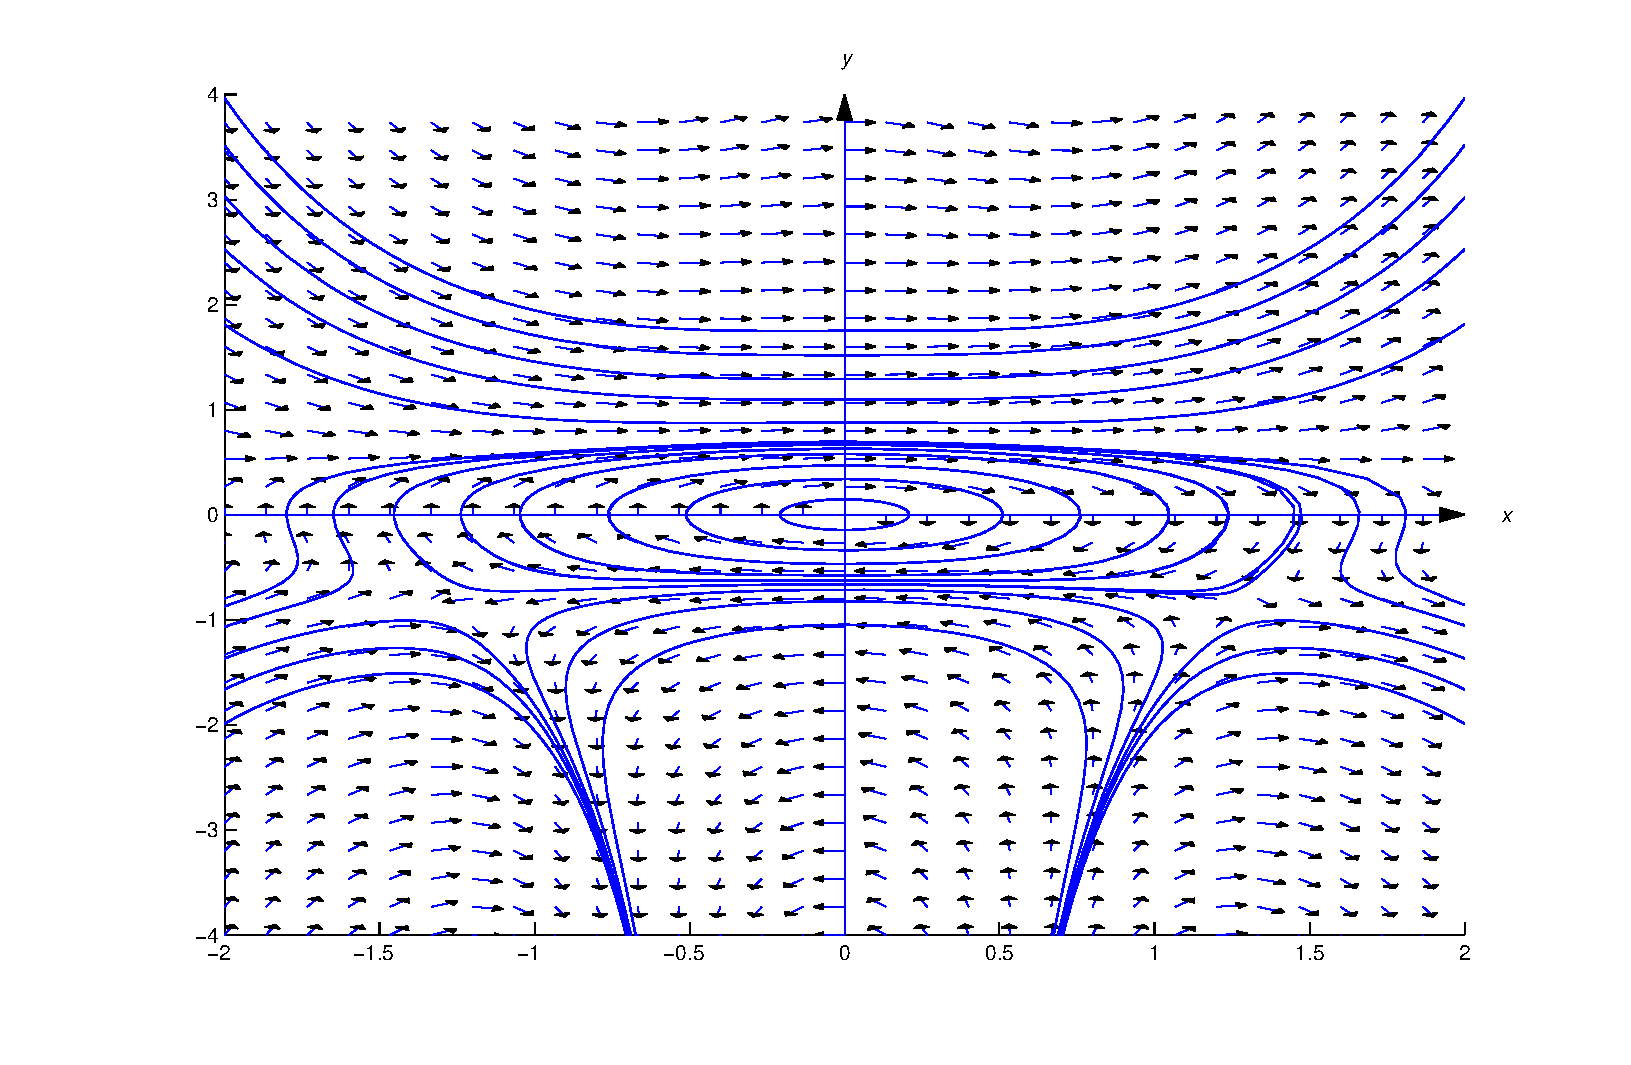
\includegraphics[bb=-78 148 689 643,width=5.67in,height=3.66in,keepaspectratio]{fig020601}
\color{blue}
\caption{A direction field and  integral curves for
$(2xy^3-2x^3y^3-4xy^2+2x)\,dx+(3x^2y^2+4y)\,dy=0$}
  \label{figure:2.6.1}
\end{figure}



\begin{example}\label{example:2.6.2}
\rm  Find an integrating factor for
\begin{equation}\label{eq:2.6.18}
2xy^3\,dx+(3x^2y^2+x^2y^3+1)\,dy=0
\end{equation}
and solve the equation.
\end{example}

\solution In \eqref{eq:2.6.18},
$$
M=2xy^3,\quad N=3x^2y^2+x^2y^3+1,
$$
and
$$
M_y-N_x=6xy^2-(6xy^2+2xy^3)=-2xy^3,
$$
so \eqref{eq:2.6.18} isn't  exact.  Moreover,
$$
{M_y-N_x\over N}=-{2xy^3\over 3x^2y^2+x^2y^2+1}
$$
is not independent of $y$, so Theorem~\ref{thmtype:2.6.1}(a) does not
apply. However,   Theorem~\ref{thmtype:2.6.1}(b) does apply, since
$$
{N_x-M_y\over M}={2xy^3\over 2xy^3}=1
$$
is independent of $x$, so we can take $q(y)=1$.
 Since
$$
\int q(y)\,dy=\int\,dy=y,
$$
  $\mu(y)=e^y$ is
an integrating factor. Multiplying \eqref{eq:2.6.18} by $\mu$ yields the
exact equation
\begin{equation}\label{eq:2.6.19}
2xy^3e^y\,dx+(3x^2y^2+x^2y^3+1)e^y\,dy=0.
\end{equation}
To solve this equation, we must find a
function $F$ such that
\begin{equation}\label{eq:2.6.20}
F_x(x,y)=2xy^3e^y
\end{equation}
 and
\begin{equation}\label{eq:2.6.21}
F_y(x,y)=(3x^2y^2+x^2y^3+1)e^y.
\end{equation}
 Integrating \eqref{eq:2.6.20} with respect to $x$ yields
\begin{equation}\label{eq:2.6.22}
F(x,y)=x^2y^3e^y+\phi(y).
\end{equation}
Differentiating this with respect to $y$ yields
$$
F_y=(3x^2y^2+x^2y^3)e^y+\phi'(y),
$$
and comparing this with \eqref{eq:2.6.21} shows that $\phi'(y)=e^y$.
 Therefore we set $\phi(y)=e^y$ in \eqref{eq:2.6.22} and conclude
that
$$
(x^2y^3+1)e^y=c
$$
is an implicit solution of \eqref{eq:2.6.19}.
It is also an implicit solution
 of \eqref{eq:2.6.18}. Figure~\ref{figure:2.6.2} shows a direction
field and some integral curves for \eqref{eq:2.6.18}.\bbox





           \begin{figure}[H]
  \centering
  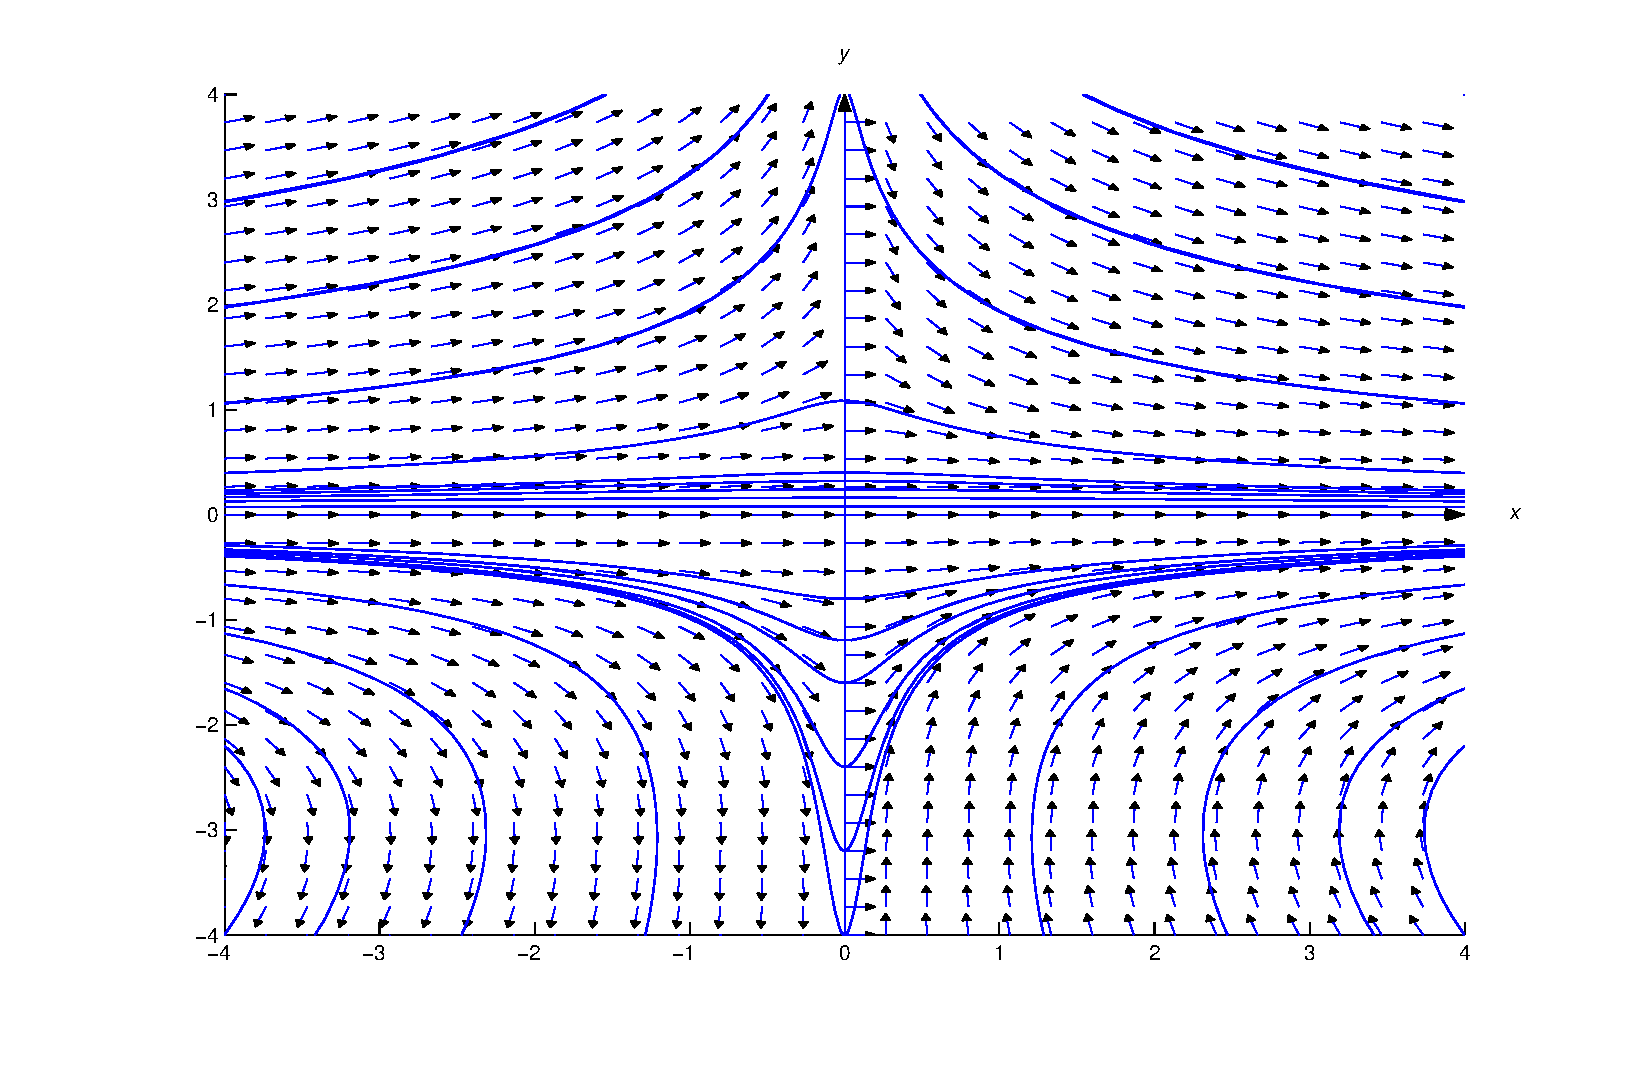
\includegraphics[bb=-78 148 689 643,width=5.67in,height=3.66in,keepaspectratio]{fig020602}
\color{blue}
\caption{
A direction field and integral curves for
$2xy^3e^y\,dx+(3x^2y^2+x^2y^3+1)e^y\,dy=0$}
  \label{figure:2.6.2}
\end{figure}


Theorem~\ref{thmtype:2.6.1} does not apply in the next example,
but the more general argument that led to Theorem~\ref{thmtype:2.6.1}
provides an integrating factor.

\begin{example}\label{example:2.6.3} \rm Find an integrating factor for
\begin{equation}\label{eq:2.6.23}
(3xy+6y^2)\,dx+(2x^2+9xy)\,dy=0
\end{equation} and solve the equation.
 \end{example}

\solution In \eqref{eq:2.6.23}
 $$
 M=3xy+6y^2,\ N=2x^2+9xy,
 $$
and
 $$
M_y-N_x=(3x+12y)-(4x+9y)=-x+3y.
$$
 Therefore
 $$ {M_y-N_x\over
M}={-x+3y\over 3xy+6y^2} \mbox{\quad and \quad} {N_x-M_y\over
N}={x-3y\over 2x^2+9xy},
 $$
so Theorem~\ref{thmtype:2.6.1} does not apply.
Following the more general argument that led to
Theorem~\ref{thmtype:2.6.1}, we look for functions $p=p(x)$ and $q=q(y)$
such that
$$
M_y-N_x=p(x)N-q(y)M;
 $$ that is,
$$
-x+3y=p(x)(2x^2+9xy)-q(y)(3xy+6y^2).
$$
Since the left side contains
only first degree terms in $x$ and $y$, we rewrite this equation as
$$
xp(x)(2x+9y)-yq(y)(3x+6y)=-x+3y.
 $$
 This will be an identity if
\begin{equation}\label{eq:2.6.24}
 xp(x)=A\mbox{\quad and\quad} yq(y)=B,
\end{equation}
 where $A$ and $B$ are constants such that
$$
-x+3y=A(2x+9y)-B(3x+6y),
 $$
 or, equivalently,
$$
-x+3y=(2A-3B)x+(9A-6B)y.
$$
Equating the coefficients of $x$ and $y$
on both sides shows that the last equation holds for all $(x,y)$ if
\begin{eqnarray*} 2A-3B &=&-1 \\ 9A-6B &=&\phantom{-}3,
\end{eqnarray*}
 which has the solution $A=1$, $B=1$. Therefore
\eqref{eq:2.6.24} implies that
 $$ p(x)={1\over x}\mbox{\quad and \quad}
q(y)={1\over y}.
$$
Since
 $$ \int p(x)\,dx=\ln|x|\mbox{\quad
and\quad}\int q(y)\,dy=\ln|y|,
$$
 we can let $P(x)=x$ and $Q(y)=y$;
hence, $\mu(x,y)=xy$ is an integrating factor. Multiplying
\eqref{eq:2.6.23} by $\mu$ yields the exact equation
$$
(3x^2y^2+6xy^3)\,dx+(2x^3y+9x^2y^2)\,dy=0.
 $$
 We leave it to you to
use the method of Section~2.5 to show that this equation has the
implicit solution
\begin{equation}
 \label{eq:2.6.25} x^3y^2+3x^2y^3=c.
\end{equation}
This is also an implicit solution of \eqref{eq:2.6.23}.
Since $x\equiv0$ and $y\equiv0$ satisfy \eqref{eq:2.6.25}, you should
check to see that $x\equiv0$ and $y\equiv0$ are also solutions of
\eqref{eq:2.6.23}. (Why is it necesary to check this?)

Figure~\ref{figure:2.6.3} shows a direction field and integral curves for
\eqref{eq:2.6.23}.


See Exercise~\ref{exer:2.6.28} for a general discussion of equations like
\eqref{eq:2.6.23}.

        \begin{figure}[tbp]
  \centering
  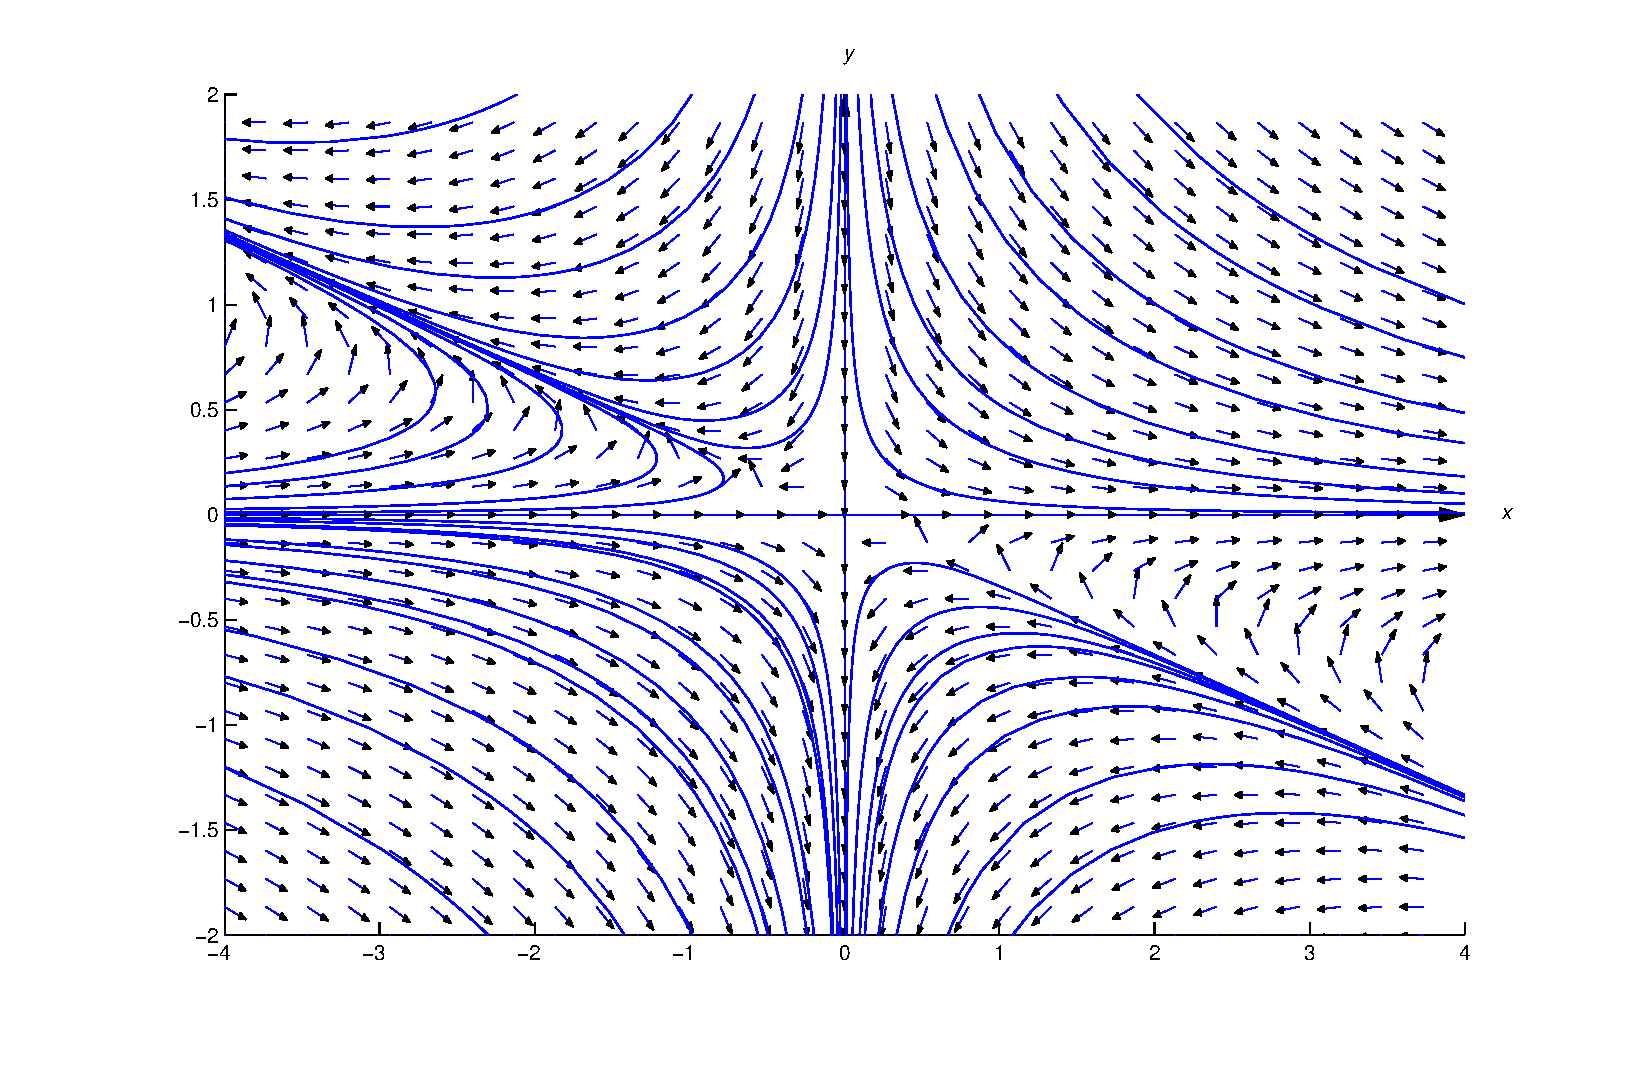
\includegraphics[bb=-78 148 689 643,width=5.67in,height=3.66in,keepaspectratio]{fig020603}
\color{blue}
\caption{
A direction field and integral curves for
$(3xy+6y^2)\,dx+(2x^2+9xy)\,dy=0$}
  \label{figure:2.6.3}
\end{figure}








\begin{example}\label{example:2.6.4}
\rm  The separable  equation
\begin{equation}\label{eq:2.6.26}
-y\,dx+(x+x^6)\,dy=0
\end{equation}
can be converted to the exact equation
\begin{equation} \label{eq:2.6.27}
-{dx\over x+x^6}+{dy\over y}=0
\end{equation}
by multiplying through
by the  integrating factor
$$
\mu(x,y)={1\over y(x+x^6)}.
$$
However, to solve \eqref{eq:2.6.27} by the method of Section~2.5
we would have to evaluate the nasty integral
$$
\int {dx\over x+x^6}.
$$
Instead, we solve \eqref{eq:2.6.26} explicitly for $y$ by finding  an
integrating factor of the form
$\mu(x,y)=x^ay^b$.
\end{example}


\begin{figure}[H]
  \centering
  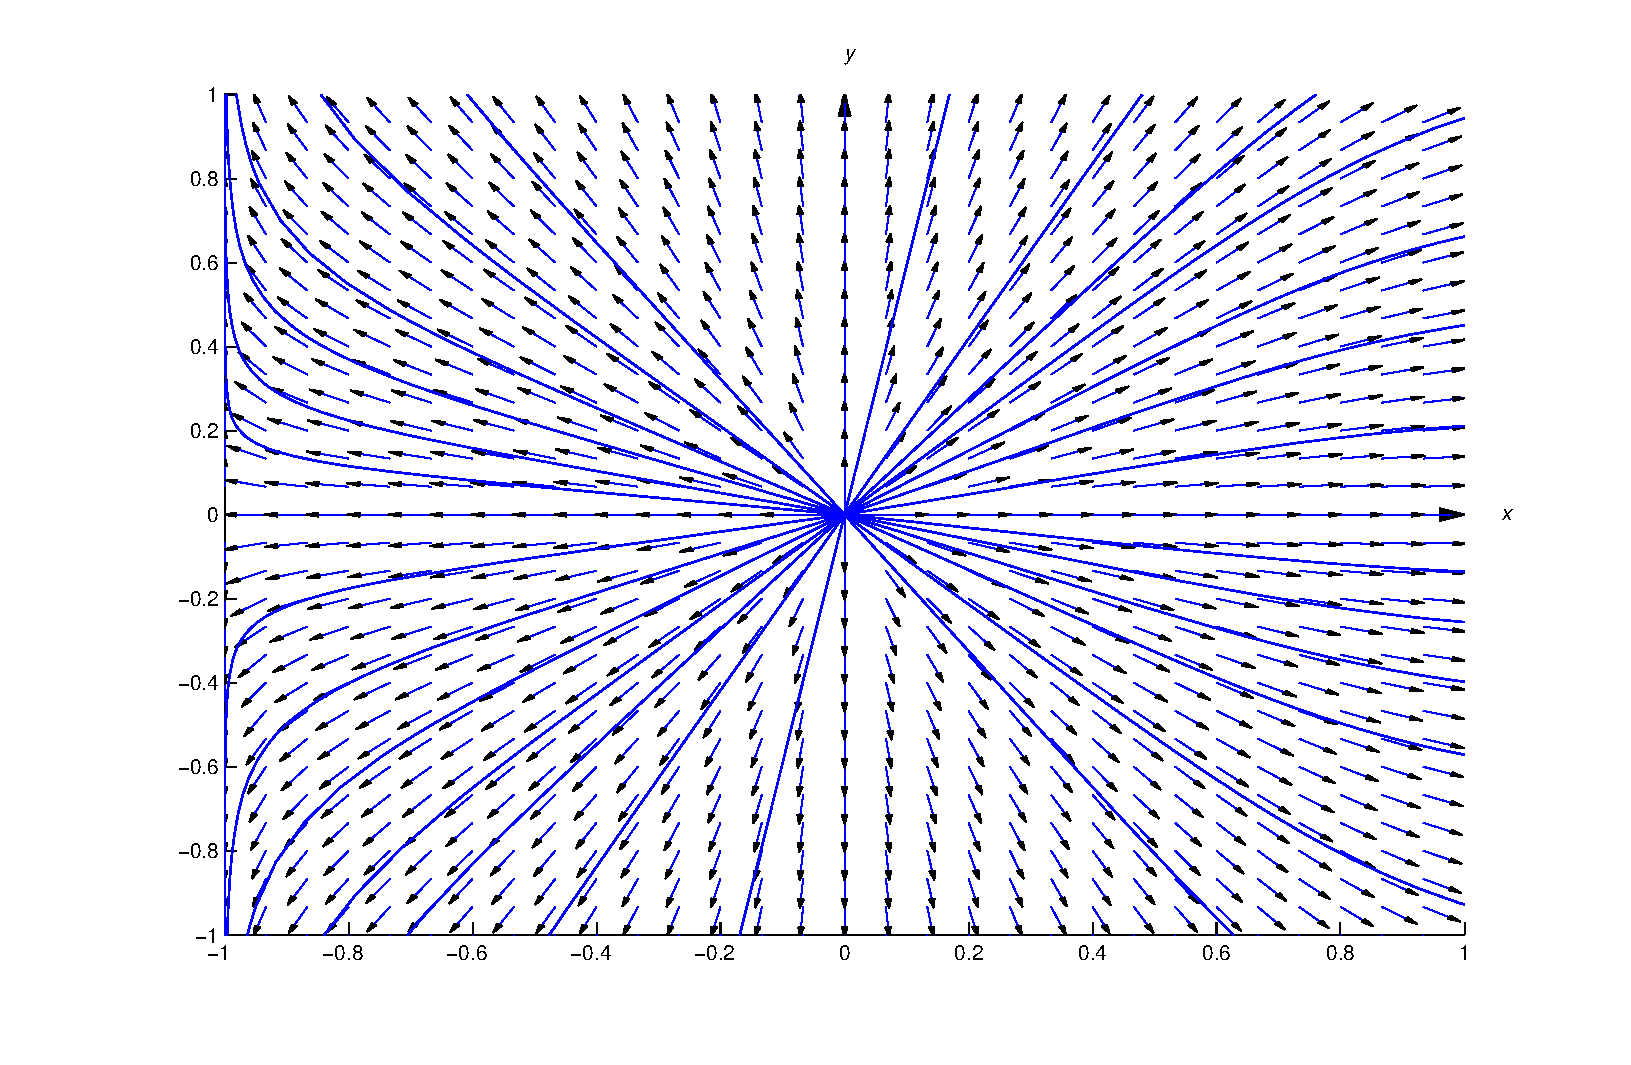
\includegraphics[bb=-78 148 689 643,width=5.67in,height=3.66in,keepaspectratio]{fig020604}
\color{blue}
\caption{A direction field and integral curves for $-y\,dx+(x+x^6)\,dy=0$}
  \label{figure:2.6.4}
\end{figure}

\solution
In \eqref{eq:2.6.26}
$$
M=-y,\ N=x+x^6,
$$
and
$$
M_y-N_x=-1-(1+6x^5)=-2-6x^5.
$$
We  look for functions
$p=p(x)$ and $q=q(y)$ such that
$$
M_y-N_x=p(x)N-q(y)M;
$$
that is,
\begin{equation}\label{eq:2.6.28}
-2-6x^5=p(x)(x+x^6)+q(y)y.
\end{equation}
The right side will contain the term $-6x^5$ if $p(x)=-6/x$.   Then
\eqref{eq:2.6.28} becomes
$$
-2-6x^5=-6-6x^5+q(y)y,
$$
so  $q(y)=4/y$.  Since
$$
\int p(x)\,dx=-\int{6\over x}\,dx=-6\ln|x|=\ln{1\over x^6},
$$
 and
$$
\int q(y)\,dy=\int{4\over y}\,dy=4\ln
|y|=\ln{y^4},
$$
we can take $P(x)=x^{-6}$ and $Q(y)=y^4$,
which yields the integrating factor $\mu(x,y)=x^{-6}y^4$.
Multiplying \eqref{eq:2.6.26} by  $\mu$ yields the exact equation
$$
-{y^5\over x^6}\,dx+\left({y^4\over x^5}+y^4\right)
\,dy=0.
$$
 We leave it to you to use the method of the Section~2.5
to show that this equation has the implicit solution $$
\left({y\over x}\right)^5+y^5=k.
$$
 Solving for $y$ yields
$$
y=k^{1/5}x(1+x^5)^{-1/5},
$$
which we rewrite as
$$
y=cx(1+x^5)^{-1/5}
$$
by renaming the arbitrary constant.
 This is also a solution of \eqref{eq:2.6.26}.

Figure~\ref{figure:2.6.4} shows a direction field and some integral curves
 for \eqref{eq:2.6.26}.






 \exercises
\begin{exerciselist}


\item\label{exer:2.6.1}
\begin{alist}
\item % (a)
Verify that $\mu(x,y)=y$ is an integrating factor for
$$
y\,dx+\left(2x+{1\over y}\right)\,dy=0
\eqno{\rm (A)}
$$
on any open rectangle that does not intersect  the $x$ axis
or, equivalently,  that
$$
y^2\,dx+(2xy+1)\,dy=0
\eqno{\rm (B)}
$$
is exact on any such rectangle.
\item % (b)
Verify that $y\equiv0$  is a solution of  (B),
but not of  (A).
\item % (b)
Show that
$$
y(xy+1)=c
\eqno{\rm (C)}
$$
is an implicit solution of (B), and explain why
every differentiable function $y=y(x)$ other than $y\equiv0$
that satisfies  (C)
 is also a solution of~(A).
\end{alist}

\item\label{exer:2.6.2}
\begin{alist}
\item % (a)
Verify that $\mu(x,y)=1/(x-y)^2$ is an integrating factor for
$$
-y^2\,dx+x^2\,dy=0
\eqno{\rm (A)}
$$
on any open rectangle  that does not intersect the line $y=x$
or, equivalently, that
$$
-{y^2\over(x-y)^2}\,dx+{x^2\over(x-y)^2}\,dy=0
\eqno{\rm (B)}
$$
is exact on any such rectangle.
\item % (b)
Use Theorem~\ref{thmtype:2.2.1} to show that
$$
{xy\over(x-y)}=c
\eqno{\rm (C)}
$$
is an implicit solution of (B), and explain why
it's also an implicit solution of (A)
\item % (b)
Verify that $y=x$  is a solution of  (A),
even though it can't be obtained from  (C).
\end{alist}

\exercisetext{In Exercises~\ref{exer:2.6.3}--\ref{exer:2.6.16} find an
integrating factor;
that is a function of only one variable, and solve the given equation.}

\begin{tabular}[t]{@{}p{168pt}@{}p{168pt}}
\item\label{exer:2.6.3} $y\,dx-x\,dy=0$ &
\item\label{exer:2.6.4} \vspace*{7.5pt} $3x^2y\,dx+2x^3\,dy=0$
\end{tabular}

\begin{tabular}[t]{@{}p{168pt}@{}p{168pt}}
\item\label{exer:2.6.5} $2y^3\,dx+3y^2\,dy=0$&
\item\label{exer:2.6.6} $(5xy+2y+5)\,dx+2x\,dy=0$
\end{tabular}

\item\label{exer:2.6.7} $(xy+x+2y+1)\,dx+(x+1)\,dy=0$

\item\label{exer:2.6.8} $(27xy^2+8y^3)\,dx+(18x^2y+12xy^2)\,dy=0$

\item\label{exer:2.6.9} $(6xy^2+2y)\,dx+(12x^2y+6x+3)\,dy=0$

\item\label{exer:2.6.10} $y^2\,dx+\dst{\left(xy^2+3xy+{1\over
y}\right)\,dy=0}$


\item\label{exer:2.6.11} $(12x^3y+24x^2y^2)\,dx+(9x^4+32x^3y+4y)\,dy=0$


\item\label{exer:2.6.12} $(x^2y+4xy+2y)\,dx+(x^2+x)\,dy=0$

\item\label{exer:2.6.13} $-y\,dx+(x^4-x)\,dy=0$

\item\label{exer:2.6.14} $\cos x\cos y\,dx
+(\sin x\cos y-\sin x\sin y+y)\,dy=0$

\item\label{exer:2.6.15} $(2xy+y^2)\,dx+(2xy+x^2-2x^2y^2-2xy^3)\,dy=0$

\item\label{exer:2.6.16} $y\sin y\,dx+x(\sin y-y\cos y)\,dy=0$

\exercisetext{In Exercises~\ref{exer:2.6.17}--\ref{exer:2.6.23} find an
integrating
factor of the form $\mu(x,y)=P(x)Q(y)$ and solve the given equation.}


\item\label{exer:2.6.17}
$y(1+5\ln|x|)\,dx+4x\ln|x|\,dy=0$

 \item\label{exer:2.6.18}
 $(\alpha y+ \gamma xy)\,dx+(\beta x+ \delta xy)\,dy=0$

\item\label{exer:2.6.19}
$(3x^2y^3-y^2+y)\,dx+(-xy+2x)\,dy=0$

\item\label{exer:2.6.20} $2y\,dx+ 3(x^2+x^2y^3)\,dy=0$

\item\label{exer:2.6.21}
$(a\cos xy-y\sin xy)\,dx+(b\cos xy-x\sin xy)\,
dy=0$

\item\label{exer:2.6.22}
$x^4y^4\,dx+x^5y^3\,dy=0$

\item\label{exer:2.6.23}
$y(x\cos x+2\sin x)\,dx+x(y+1)\sin x\,dy=0$


\exercisetext{In Exercises~\ref{exer:2.6.24}--\ref{exer:2.6.27} find an
integrating factor
and solve the  equation. Plot a direction field and some
integral curves for the equation in the indicated rectangular region.}

\item\label{exer:2.6.24} \CGex
 $(x^4y^3+y)\,dx+(x^5y^2-x)\,dy=0;   \quad \{-1\le x\le1,-1\le y\le1\}$


\item\label{exer:2.6.25} \CGex
$(3xy+2y^2+y)\,dx+(x^2+2xy+x+2y)\,dy=0;   \quad \{-2\le x\le2,-2\le
y\le2\}$


\item\label{exer:2.6.26} \CGex
$(12 xy+6y^3)\,dx+(9x^2+10xy^2)\,dy=0;   \quad \{-2\le x\le2,-2\le y\le2\}$

\item\label{exer:2.6.27} \CGex
$(3x^2y^2+2y)\,dx+ 2x\,dy=0;   \quad \{-4\le x\le4,-4\le y\le4\}$




\item\label{exer:2.6.28}
Suppose $a$, $b$, $c$, and $d$ are constants such that
$ad-bc\ne0$, and let $m$ and $n$ be arbitrary real numbers.
Show that
$$
(ax^my+by^{n+1})\,dx+(cx^{m+1}+dxy^n)\,dy=0
$$
has an integrating factor $\mu(x,y)=x^\alpha y^\beta$.

\item\label{exer:2.6.29}
Suppose $M$, $N$, $M_x$, and $N_y$  are continuous for all
$(x,y)$, and $\mu=\mu(x,y)$  is an integrating factor for
$$
M(x,y)\,dx+N(x,y)\,dy=0.
\eqno{\rm (A)}
$$
Assume that $\mu_x$ and $\mu_y$ are continuous for all $(x,y)$, and
suppose   $y=y(x)$ is a differentiable function such that
$\mu(x,y(x))=0$ and $\mu_x(x,y(x))\ne0$ for all $x$ in some interval
$I$. Show that $y$ is a solution of (A) on $I$.

\item\label{exer:2.6.30}
According to Theorem~\ref{thmtype:2.1.2}, the general solution of the
linear nonhomogeneous equation
$$
y'+p(x)y=f(x)
\eqno{\rm(A)}
$$
is
$$
y=y_1(x)\left(c+\int f(x)/y_1(x)\,dx\right),
\eqno{\rm(B)}
$$
where $y_1$ is any nontrivial solution of the
complementary equation $y'+p(x)y=0$. In this exercise we obtain this
conclusion in a different way.
You may find it instructive to apply the method suggested here
to solve some of the exercises in Section~2.1.
\begin{alist}
\item % (a)
Rewrite (A) as
$$
[p(x)y-f(x)]\,dx+\,dy=0,
\eqno{\rm(C)}
$$
and show that $\mu=\pm e^{\int p(x)\,dx}$ is an integrating factor
for (C).
\item % (b)
Multiply (A) through by $\mu=\pm e^{\int p(x)\,dx}$  and verify that
the resulting equation can be rewritten as
$$
(\mu(x)y)'=\mu(x)f(x).
$$
Then integrate both sides of this equation and solve for $y$
to show that the general solution of (A) is
$$
y={1\over\mu(x)}\left(c+\int f(x)\mu(x)\,dx\right).
$$
Why is this form of the general solution
 equivalent to (B)?
\end{alist}

\end{exerciselist}




\newpage
\thispagestyle{empty}
\mbox{}
\newpage
\thispagestyle{empty}




\setcounter{chapter}{3}
\pdfbookmark[0]{Chapter 3 Numerical Methods}{chapter:3}
\chaptertitle{Numerical Methods}

\noindent
In this chapter we study numerical methods for solving a first order
differential equation
$$
y'=f(x,y).
$$


\medskip\noindent
SECTION~3.1 deals with
\href{http://www-history.mcs.st-and.ac.uk/Mathematicians/Euler.html}
{\color{blue}\it Euler's
  method}, which is
really too crude to be of much use in practical applications. However,
its simplicity allows for an introduction to the ideas required to
understand the better methods discussed in the other two sections.

\medskip\noindent
SECTION~3.2 discusses improvements on Euler's method.


\medskip\noindent
SECTION~3.3 deals with the
\href{http://www-history.mcs.st-and.ac.uk/Mathematicians/Runge.html}
{Runge\color{blue}}-\href{http://www-history.mcs.st-and.ac.uk/Mathematicians/Kutta.html}
{\color{blue}Kutta}
method, perhaps
the most widely used method for numerical solution of differential
equations.
 \vspace*{4in}

\centerline{95}

\newpage
\newsection{1}{Numerical Methods}{Euler's Method}
\subpdfbookmark{Section 3.1 Euler's Method} {section:3.1}
\vskip14pt

\renewcommand{\thissection}{\sectiontitle{\, EULER'S METHOD}}
\thissection

\noindent
If an initial value problem
\begin{equation} \label{eq:3.1.1}
y'=f(x,y),\quad y(x_0)=y_0
 \end{equation}
can't be solved analytically,
 it's necessary to resort to
numerical methods to obtain useful  approximations to a solution of
\eqref{eq:3.1.1}. We'll consider such methods in this chapter.

We're interested in
computing approximate values of the solution of \eqref{eq:3.1.1} at
equally spaced points $x_0$, $x_1$, \dots, $x_n=b$ in an interval
$[x_0,b]$.
 Thus,
$$
x_i=x_0+ih,\quad i=0,1, \dots,n,
$$
where
$$
h={b-x_0\over n}.
$$
We'll denote the approximate values of the solution at these points
by $y_0$, $y_1$, \dots, $y_n$;   thus, $y_i$ is an approximation to
$y(x_i)$.
We'll call
$$
e_i=y(x_i)-y_i
$$
the {\color{blue}\it  error at the $i$th step.\/} Because of the initial
condition
$y(x_0)=y_0$, we'll always have $e_0=0$. However, in general
$e_i\ne0$ if $i>0$.

We encounter two sources of error
in applying a numerical method to solve an initial value problem:
\begin{itemize}
\item
The formulas defining the method are based on some sort of
approximation. Errors due to the inaccuracy of the approximation are
called {\color{blue}\it truncation errors\/}.
\item
Computers do arithmetic with a fixed number of digits, and therefore
make errors in evaluating the formulas defining the numerical methods.
Errors due to the computer's inability to do exact arithmetic are
called {\color{blue}\it roundoff errors.\/}
\end{itemize}


Since a careful analysis of roundoff error is beyond the scope of this
book, we'll consider only truncation errors.

\boxit{Euler's Method}


\noindent
The simplest numerical method for solving \eqref{eq:3.1.1} is
\href{http://www-history.mcs.st-and.ac.uk/Mathematicians/Euler.html}
{\color{blue}\it
Euler's method\/}.
This method is so crude that it
is seldom used in practice;     however, its simplicity makes it useful
for illustrative purposes.

Euler's method is based on the assumption that the tangent line to the
integral curve of \eqref{eq:3.1.1} at $(x_i,y(x_i))$ approximates the
integral curve over the interval $[x_i,x_{i+1}]$.
 Since the slope of the integral curve of
\eqref{eq:3.1.1} at $(x_i,y(x_i))$ is $y'(x_i)=f(x_i,y(x_i))$, the
equation of the tangent line to the integral curve at $(x_i,y(x_i))$
is
\begin{equation} \label{eq:3.1.2}
y=y(x_i)+f(x_i,y(x_i))(x-x_i).
\end{equation}

Setting $x=x_{i+1}=x_i+h$ in \eqref{eq:3.1.2} yields
\begin{equation} \label{eq:3.1.3}
y_{i+1}=y(x_i)+hf(x_i,y(x_i))
\end{equation}
as an approximation to $y(x_{i+1})$. Since $y(x_0)=y_0$ is known, we
can use \eqref{eq:3.1.3} with $i=0$ to compute
$$
y_1=y_0+hf(x_0,y_0).
$$
However, setting $i=1$ in \eqref{eq:3.1.3} yields
$$
y_2=y(x_1)+hf(x_1,y(x_1)),
$$
which isn't  useful, since we {\color{blue}\it don't know\/} $y(x_1)$. Therefore
we replace $y(x_1)$ by its approximate value $y_1$ and redefine
$$
y_2=y_1+hf(x_1,y_1).
$$
Having computed $y_2$, we can  compute
$$
y_3=y_2+hf(x_2,y_2).
$$
In general, Euler's method starts with the known value $y(x_0)=y_0$
and computes $y_1$, $y_2$, \dots, $y_n$ successively by with the
 formula
\begin{equation} \label{eq:3.1.4}
y_{i+1}=y_i+hf(x_i,y_i),\quad 0\le i\le n-1.
\end{equation}

The next example illustrates the computational procedure
indicated in Euler's method.

\begin{example}\label{example:3.1.1} \rm
Use Euler's method with $h=0.1$ to find approximate values for the
solution of the initial value problem
\begin{equation}\label{eq:3.1.5}
y'+2y=x^3e^{-2x},\quad y(0)=1
\end{equation}
at $x=0.1,0.2,0.3$.
\end{example}

\solution
We rewrite \eqref{eq:3.1.5}  as
$$
y'=-2y+x^3e^{-2x},\quad y(0)=1,
$$
which is of the form \eqref{eq:3.1.1}, with
$$
f(x,y)=-2y+x^3e^{-2x},\ x_0=0,\mbox{\ and}\ y_0=1.
$$
Euler's method yields
\begin{eqnarray*}
y_1 & = & y_0+hf(x_0,y_0)\\
 & = & 1+(.1)f(0,1)=1+(.1)(-2)=.8,\\[4\jot]
y_2 & = & y_1+hf(x_1,y_1)\\
 & = & .8+(.1)f(.1,.8)=.8+(.1)\left(-2(.8)+(.1)^3e^{-.2}\right)=
.640081873,\\[4\jot]
y_3 & = & y_2+hf(x_2,y_2)\\
 & = & .640081873+(.1)\left(-2(.640081873)+(.2)^3e^{-.4}\right)=
.512601754.\bbox
\end{eqnarray*}

We've written the details of these computations to ensure that you
understand the procedure. However,  in the rest of the examples as
well as
 the exercises  in this chapter, we'll assume that you can use a
programmable calculator or a computer
to carry out the necessary computations.

\medskip
\boxit{Examples Illustrating The Error in Euler's Method}


\begin{example}\label{example:3.1.2} \rm
Use Euler's method with step sizes $h=0.1$, $h=0.05$, and $h=0.025$ to
find approximate values of the solution of the initial value problem
$$
y'+2y=x^3e^{-2x},\quad y(0)=1
$$
at $x=0$, $0.1$, $0.2$, $0.3$, \dots, $1.0$. Compare these approximate
values
with the values of the exact solution
\begin{equation} \label{eq:3.1.6}
y={e^{-2x}\over4}(x^4+4),
\end{equation}
which can be obtained by the method of Section~2.1. (Verify.)
\end{example}


\solution Table~\ref{table:3.1.1} shows the values of the exact solution
\eqref{eq:3.1.6} at the specified points, and the approximate values of
the solution at these points obtained by Euler's method with step
sizes $h=0.1$, $h=0.05$, and $h=0.025$. In examining this table, keep
in mind that the approximate values in the column corresponding to
$h=.05$ are actually the results of 20 steps with Euler's method. We
haven't listed the estimates of the solution obtained for
$x=0.05$, $0.15$, \dots, since there's nothing to compare them with in
the column corresponding to $h=0.1$. Similarly, the approximate values
in the column corresponding to $h=0.025$ are actually the results of
40 steps with Euler's method.

\begin{newtable} \label{table:3.1.1}
{Numerical solution of
$y'+2y=x^3e^{-2x},\ y(0)=1$, by Euler's method.}
\begin{center}
\begin{tabular}{|c|r|r|r|r|}
\hline
\multicolumn{1}{|c|}{$x$}&
\multicolumn{1}{|c|}{$h=0.1$}&
\multicolumn{1}{|c|}{$h=0.05$}&
\multicolumn{1}{|c|}{$h=0.025$}&
\multicolumn{1}{|c|}{Exact}\\ \hline
0.0 & 1.000000000 & 1.000000000 & 1.000000000 & 1.000000000 \\
0.1 & 0.800000000 & 0.810005655 & 0.814518349 & 0.818751221 \\
0.2 & 0.640081873 & 0.656266437 & 0.663635953 & 0.670588174 \\
0.3 & 0.512601754 & 0.532290981 & 0.541339495 & 0.549922980 \\
0.4 & 0.411563195 & 0.432887056 & 0.442774766 & 0.452204669 \\
0.5 & 0.332126261 & 0.353785015 & 0.363915597 & 0.373627557 \\
0.6 & 0.270299502 & 0.291404256 & 0.301359885 & 0.310952904 \\
0.7 & 0.222745397 & 0.242707257 & 0.252202935 & 0.261398947 \\
0.8 & 0.186654593 & 0.205105754 & 0.213956311 & 0.222570721 \\
0.9 & 0.159660776 & 0.176396883 & 0.184492463 & 0.192412038 \\
1.0 & 0.139778910 & 0.154715925 & 0.162003293 & 0.169169104\\
\hline
\end{tabular}
\end{center}
\end{newtable}

You can see from Table~\ref{table:3.1.1} that decreasing the step size
improves the accuracy of Euler's method. For example,
$$
y_{\mbox{\tiny exact}}(1)-y_{\mbox{\tiny approx}}(1)\approx
\left\{\begin{array}{l}
.0293\mbox{ with }h=0.1,\\
.0144\mbox{ with }h=0.05,\\
.0071\mbox{ with }h=0.025.
\end{array}\right.
$$
Based on this scanty evidence, you might guess that the error in
approximating the exact solution at a {\color{blue}\it fixed value of\/} $x$ by
Euler's method is roughly halved when the step size is halved. You can
find more evidence to support this conjecture by examining
Table~\ref{table:3.1.2}, which lists the approximate values of
$y_{\mbox{\tiny exact}}-y_{\mbox{\tiny approx}}$ at
$x=0.1$, $0.2$, \dots, $1.0$.

\begin{newtable} \label{table:3.1.2}
{Errors in approximate solutions of $y'+2y=x^3e^{-2x},\
y(0)=1$, obtained by Euler's method.}
\begin{center}
\begin{tabular}{|c|r|r|r|}
\hline
\multicolumn{1}{|c|}{$x$}&
\multicolumn{1}{|c|}{$h=0.1$}&
\multicolumn{1}{|c|}{$h=0.05$}&
\multicolumn{1}{|c|}{$h=0.025$}\\ \hline
0.1 & 0.0187 & 0.0087 & 0.0042\\
0.2 & 0.0305 & 0.0143 & 0.0069\\
0.3 & 0.0373 & 0.0176 & 0.0085\\
0.4 & 0.0406 & 0.0193 & 0.0094\\
0.5 & 0.0415 & 0.0198 & 0.0097\\
0.6 & 0.0406 & 0.0195 & 0.0095\\
0.7 & 0.0386 & 0.0186 & 0.0091\\
0.8 & 0.0359 & 0.0174 & 0.0086\\
0.9 & 0.0327 & 0.0160 & 0.0079\\
1.0 & 0.0293 & 0.0144 & 0.0071\\
\hline
\end{tabular}
\end{center}
\end{newtable}

\begin{example}\label{example:3.1.3} \rm
Tables~\ref{table:3.1.3} and \ref{table:3.1.4} show analogous results
for the nonlinear initial value problem
\begin{equation} \label{eq:3.1.7}
y'=-2y^2+xy+x^2,\ y(0)=1,
\end{equation}
except in this case we can't solve \eqref{eq:3.1.7} exactly.
The results in the ``Exact'' column were obtained by using a
more accurate numerical method known as the
\href{http://www-history.mcs.st-and.ac.uk/Mathematicians/Runge.html}
{\color{blue}\it Runge}-\href{http://www-history.mcs.st-and.ac.uk/Mathematicians/Kutta.html}{\it\color{blue}Kutta\/}
method
 with a small step size. They are
exact to eight decimal places.\bbox
\end{example}


Since we think it's important in evaluating the accuracy of the
numerical methods that we'll be studying in this chapter, we
often include a column listing values of the exact solution of the
initial value problem, even if the directions in the example or
exercise don't specifically call for it. If  quotation marks are
included in the heading, the values were obtained by applying the
Runge-Kutta method in a way that's explained in Section~3.3.
If  quotation marks are not included,  the values were
obtained from a known formula for the solution.
In either case, the values are exact to eight places to the
right of the decimal point.



\begin{newtable} \label{table:3.1.3}
{Numerical solution of
$y'=-2y^2+xy+x^2,\ y(0)=1$, by Euler's method.}
\begin{center}
\begin{tabular}{|c|r|r|r|r|}
\hline
\multicolumn{1}{|c|}{$x$}&
\multicolumn{1}{|c|}{$h=0.1$}&
\multicolumn{1}{|c|}{$h=0.05$}&
\multicolumn{1}{|c|}{$h=0.025$}&
\multicolumn{1}{|c|}{``Exact''}\\ \hline
0.0 & 1.000000000 & 1.000000000 & 1.000000000 & 1.000000000 \\
0.1 & 0.800000000 & 0.821375000 & 0.829977007 & 0.837584494 \\
0.2 & 0.681000000 & 0.707795377 & 0.719226253 & 0.729641890 \\
0.3 & 0.605867800 & 0.633776590 & 0.646115227 & 0.657580377 \\
0.4 & 0.559628676 & 0.587454526 & 0.600045701 & 0.611901791 \\
0.5 & 0.535376972 & 0.562906169 & 0.575556391 & 0.587575491 \\
0.6 & 0.529820120 & 0.557143535 & 0.569824171 & 0.581942225 \\
0.7 & 0.541467455 & 0.568716935 & 0.581435423 & 0.593629526 \\
0.8 & 0.569732776 & 0.596951988 & 0.609684903 & 0.621907458 \\
0.9 & 0.614392311 & 0.641457729 & 0.654110862 & 0.666250842 \\
1.0 & 0.675192037 & 0.701764495 & 0.714151626 & 0.726015790\\
\hline
\end{tabular}
\end{center}
\end{newtable}

\begin{newtable} \label{table:3.1.4}
{Errors in approximate solutions of $y'=-2y^2+xy+x^2,\
y(0)=1$, obtained by Euler's method.}
\begin{center}
\begin{tabular}{|c|r|r|r|}
\hline
\multicolumn{1}{|c|}{$x$}&
\multicolumn{1}{|c|}{$h=0.1$}&
\multicolumn{1}{|c|}{$h=0.05$}&
\multicolumn{1}{|c|}{$h=0.025$}\\ \hline
0.1 & 0.0376 & 0.0162 &0.0076 \\
0.2 & 0.0486 & 0.0218 &0.0104 \\
0.3 & 0.0517 & 0.0238 &0.0115 \\
0.4 & 0.0523 & 0.0244 &0.0119 \\
0.5 & 0.0522 & 0.0247 &0.0121 \\
0.6 & 0.0521 & 0.0248 &0.0121 \\
0.7 & 0.0522 & 0.0249 &0.0122 \\
0.8 & 0.0522 & 0.0250 &0.0122 \\
0.9 & 0.0519 & 0.0248 &0.0121 \\
1.0 & 0.0508 & 0.0243 &0.0119 \\
\hline
\end{tabular}
\end{center}
\end{newtable}


\boxit{Truncation Error in Euler's Method}


\noindent
Consistent with the results indicated in
Tables~\ref{table:3.1.1}--\ref{table:3.1.4}, we'll now show that under
reasonable assumptions on $f$ there's a constant $K$ such that
the error in approximating the solution of the initial value problem
$$
y'=f(x,y),\quad y(x_0)=y_0,
$$
at a given point $b>x_0$ by Euler's method with step size
$h=(b-x_0)/n$ satisfies the inequality
$$
|y(b)-y_n|\le Kh,
$$
where $K$ is a constant independent of $n$.


There are two sources of error (not counting roundoff) in Euler's
method:
\begin{numberlist}
\item % (1)
The error committed in approximating the integral curve by the tangent
line \eqref{eq:3.1.2} over the interval $[x_i,x_{i+1}]$.
\item % (2)
The error committed in replacing $y(x_i)$ by $y_i$ in
\eqref{eq:3.1.2} and using \eqref{eq:3.1.4} rather than \eqref{eq:3.1.2} to
compute $y_{i+1}$.
 \end{numberlist}

Euler's method assumes that $y_{i+1}$ defined in \eqref{eq:3.1.2}  is
an approximation to $y(x_{i+1})$. We call the error in this
approximation the {\color{blue}\it local truncation error at the $i$th step\/},
and denote it by $T_i$;   thus,
\begin{equation} \label{eq:3.1.8}
T_i=y(x_{i+1})-y(x_i)-hf(x_i,y(x_i)).
\end{equation}
We'll now use
\href{http://www-history.mcs.st-and.ac.uk/Mathematicians/Taylor.html}
{\color{blue}\it Taylor's theorem\/}
 to estimate $T_i$, assuming for
simplicity that $f$, $f_x$, and $f_y$ are continuous and bounded for
all $(x,y)$. Then $y''$ exists and is bounded on $[x_0,b]$. To see
this, we differentiate
$$
y'(x)=f(x,y(x))
$$
to obtain
\begin{eqnarray*}
y''(x) & = & f_x(x,y(x))+f_y(x,y(x))y'(x)\\
 & = & f_x(x,y(x))+f_y(x,y(x))f(x,y(x)).
\end{eqnarray*}
Since we assumed that $f$, $f_x$ and $f_y$ are bounded, there's
a constant $M$ such that
$$
|f_x(x,y(x))+f_y(x,y(x))f(x,y(x))|\le M,\quad x_0<x<b,
$$
which implies that
\begin{equation} \label{eq:3.1.9}
|y''(x)|\le M,\quad x_0<x<b.
\end{equation}
Since $x_{i+1}=x_i+h$, Taylor's theorem implies that
$$
y(x_{i+1})=y(x_i)+hy'(x_i)+{h^2\over2}y''(\tilde x_i),
$$
where $\tilde x_i$ is some number between $x_i$ and $x_{i+1}$.
Since $y'(x_i)=f(x_i,y(x_i))$  this can be written as
$$
y(x_{i+1})=y(x_i)+hf(x_i,y(x_i))+{h^2\over2}y''(\tilde x_i),
$$
or, equivalently,
$$
y(x_{i+1})-y(x_i)-hf(x_i,y(x_i))={h^2\over2}y''(\tilde x_i).
$$
Comparing this with \eqref{eq:3.1.8} shows that
$$
T_i={h^2\over2}y''(\tilde x_i).
$$
Recalling \eqref{eq:3.1.9}, we can establish the bound
\begin{equation} \label{eq:3.1.10}
|T_i|\le{Mh^2\over2},\quad 1\le i\le n.
\end{equation}
Although it may be difficult to determine the constant $M$, what is
important is that there's an $M$ such that \eqref{eq:3.1.10} holds.
 We say that the
local truncation error of Euler's method is {\color{blue}\it  of order\/} $h^2$,
which we write as $O(h^2)$.

Note that the magnitude of the local truncation error in
Euler's method is determined by the second derivative $y''$ of the
solution of the initial value problem. Therefore
 the local truncation error will be larger where $|y''|$ is large,
or smaller where $|y''|$ is small.

Since the local truncation error for Euler's method is $O(h^2)$, it's
reasonable to expect that halving $h$ reduces the local truncation
error by a factor of 4. This is true, but
 halving the step size also requires twice as many steps to
approximate the solution at a given point. To analyze the overall
effect of truncation error in Euler's method, it's useful to  derive
an equation relating the errors
$$
e_{i+1}=y(x_{i+1})-y_{i+1}\mbox{\quad and \quad} e_i=y(x_i)-y_i.
$$
To this end, recall that
\begin{equation} \label{eq:3.1.11}
y(x_{i+1})=y(x_i)+hf(x_i,y(x_i))+T_i
\end{equation}
and
\begin{equation} \label{eq:3.1.12}
y_{i+1}=y_i+hf(x_i,y_i).
\end{equation}
Subtracting \eqref{eq:3.1.12} from \eqref{eq:3.1.11} yields
\begin{equation} \label{eq:3.1.13}
e_{i+1}=e_i+h\left[f(x_i,y(x_i))-f(x_i,y_i)\right]+T_i.
\end{equation}
The last term on the right is the local truncation error at the $i$th
step. The other terms reflect the way errors made at {\color{blue}\it previous
steps\/} affect $e_{i+1}$. Since $|T_i|\le Mh^2/2$, we see from
\eqref{eq:3.1.13} that
\begin{equation} \label{eq:3.1.14}
|e_{i+1}|\le |e_i|+h|f(x_i,y(x_i))-f(x_i,y_i)|+{Mh^2\over2}.
\end{equation}
Since we assumed that $f_y$ is continuous and bounded, the mean
value theorem implies that
$$
f(x_i,y(x_i))-f(x_i,y_i)=f_y(x_i,y_i^*)(y(x_i)-y_i)=f_y(x_i,y_i^*)e_i,
$$
where $y_i^*$ is between $y_i$ and $y(x_i)$. Therefore
$$
|f(x_i,y(x_i))-f(x_i,y_i)|\le R|e_i|
$$
for some constant $R$. From this and \eqref{eq:3.1.14},
\begin{equation} \label{eq:3.1.15}
|e_{i+1}|\le (1+Rh)|e_i|+{Mh^2\over2},\quad 0\le i\le n-1.
\end{equation}
For convenience, let $C=1+Rh$. Since $e_0=y(x_0)-y_0=0$, applying
\eqref{eq:3.1.15} repeatedly yields
\begin{eqnarray}
|e_1| & \le & {Mh^2\over2}\nonumber\\
|e_2| & \le & C|e_1|+{Mh^2\over2}\le(1+C){Mh^2\over2}\nonumber\\
|e_3| & \le & C|e_2|+{Mh^2\over2}\le(1+C+C^2){Mh^2\over2}\nonumber\\
 & \vdots &\nonumber \\|e_n| & \le &
C|e_{n-1}|+{Mh^2\over2}\le(1+C+\cdots+C^{n-1}){Mh^2\over2}.\label{eq:3.1.16}
\end{eqnarray}

Recalling the formula for the sum of a geometric series, we see that
$$
1+C+\cdots+C^{n-1}={1-C^n\over 1-C}={(1+Rh)^n-1\over Rh}
$$
(since $C=1+Rh$). From this and \eqref{eq:3.1.16},
\begin{equation} \label{eq:3.1.17}
|y(b)-y_n|=|e_n|\le{(1+Rh)^n-1\over R}{Mh\over2}.
\end{equation}
Since Taylor's theorem implies that
$$
1+Rh<e^{Rh}
$$
(verify),
$$
(1+Rh)^n<e^{nRh}=e^{R(b-x_0)}\quad (\mbox{since }nh=b-x_0).
$$
This and \eqref{eq:3.1.17} imply that
\begin{equation} \label{eq:3.1.18}
|y(b)-y_n|\le Kh,
\end{equation}
with
$$
K=M{e^{R(b-x_0)}-1\over2R}.
$$
Because of \eqref{eq:3.1.18} we say that the
\href{http://www-history.mcs.st-and.ac.uk/Mathematicians/Euler.html}
{\color{blue}\it global truncation
error of Euler's method is of order\/} $h$, which we write as $O(h)$.

\boxit{Semilinear Equations and Variation of Parameters}


\noindent
An equation that can be written in the form
\begin{equation} \label{eq:3.1.19}
y'+p(x)y=h(x,y)
\end{equation}
with $p\not\equiv0$ is said to be {\color{blue}\it semilinear\/}. (Of course,
\eqref{eq:3.1.19} is linear if $h$ is independent of $y$.) One way to
apply Euler's method to an initial value problem
\begin{equation} \label{eq:3.1.20}
y'+p(x)y=h(x,y),\quad y(x_0)=y_0
\end{equation}
for \eqref{eq:3.1.19} is to think of it  as
$$
y'=f(x,y),\quad y(x_0)=y_0,
$$
where
$$
f(x,y)=-p(x)y+h(x,y).
$$
However, we can also start by applying variation of parameters to
\eqref{eq:3.1.20}, as in Sections~2.1\ and 2.4;   thus, we
write the solution of \eqref{eq:3.1.20} as $y=uy_1$, where $y_1$ is a
nontrivial solution of the complementary equation $y'+p(x)y=0$. Then
$y=uy_1$ is a solution of \eqref{eq:3.1.20} if and only if $u$ is a
solution of the initial value problem
\begin{equation} \label{eq:3.1.21}
u'=h(x,uy_1(x))/y_1(x),\quad u(x_0)=y(x_0)/y_1(x_0).
\end{equation}
We can apply Euler's method to obtain approximate values
$u_0$, $u_1$, \dots, $u_n$ of this initial value problem, and then take
$$
y_i=u_iy_1(x_i)
$$
as approximate values of the solution of \eqref{eq:3.1.20}.
We'll call this procedure the
\href{http://www-history.mcs.st-and.ac.uk/Mathematicians/Euler.html}
{\color{blue}\it  Euler semilinear method\/}.

The next two examples show that the Euler and Euler semilinear
methods may yield drastically different results.

\enlargethispage{3in}

\begin{example}\label{example:3.1.4} \rm
In Example~\ref{example:2.1.7} we had to leave the solution of the initial
value
problem
\begin{equation} \label{eq:3.1.22}
y'-2xy=1,\quad y(0)=3
\end{equation}
in the  form
\begin{equation} \label{eq:3.1.23}
y=e^{x^2}\left(3 +\int^x_0 e^{-t^2}dt\right)
\end{equation}
\newpage
\noindent
because it was impossible to evaluate this integral exactly in terms
of elementary functions.
Use step sizes $h=0.2$, $h=0.1$, and $h=0.05$ to find approximate
values
of the solution of \eqref{eq:3.1.22} at $x=0$, $0.2$, $0.4$, $0.6$,
\dots, $2.0$ by
{\bf (a)} Euler's method;   {\bf (b)} the Euler semilinear method.
\end{example}


\solutionpart{a}
Rewriting \eqref{eq:3.1.22} as
\begin{equation} \label{eq:3.1.24}
y'=1+2xy,\quad y(0)=3
\end{equation}
and applying Euler's method with $f(x,y)=1+2xy$ yields the results
shown in Table~\ref{table:3.1.5}. Because of the large differences
between the estimates obtained for the three values of $h$, it
would be clear that these results are useless even if the ``exact''
values were not included in the table.

\begin{newtable} \label{table:3.1.5}
{Numerical solution of
$y'-2xy=1,\ y(0)=3$, with Euler's method.}
\begin{center}
\begin{tabular}{|c|r|r|r|r|}
\hline
\multicolumn{1}{|c|}{$x$}&
\multicolumn{1}{|c|}{$h=0.2$}&
\multicolumn{1}{|c|}{$h=0.1$}&
\multicolumn{1}{|c|}{$h=0.05$}&
\multicolumn{1}{|c|}{``Exact''}\\ \hline
0.0 &  3.000000000 & 3.000000000 & 3.000000000     &   3.000000000 \\
0.2 &  3.200000000 & 3.262000000 &3.294348537      &   3.327851973 \\
0.4 &  3.656000000 & 3.802028800 & 3.881421103     &   3.966059348 \\
0.6 &  4.440960000 & 4.726810214 & 4.888870783     &   5.067039535 \\
0.8 &  5.706790400 & 6.249191282 & 6.570796235     &   6.936700945 \\
1.0 &  7.732963328 & 8.771893026 & 9.419105620     &  10.184923955 \\
1.2 & 11.026148659 &13.064051391 &14.405772067     &  16.067111677 \\
1.4 & 16.518700016 &20.637273893 & 23.522935872    &  27.289392347 \\
1.6 & 25.969172024 &34.570423758 & 41.033441257    &  50.000377775 \\
1.8 & 42.789442120 &61.382165543 & 76.491018246    &  98.982969504 \\
2.0 & 73.797840446 & 115.440048291 & 152.363866569 & 211.954462214 \\
\hline
\end{tabular}
\end{center}
\end{newtable}


It's easy to see why Euler's method yields such poor results.
Recall that the constant $M$ in
\eqref{eq:3.1.10} -- which plays an important role in determining the
local truncation error in Euler's method -- must be an upper bound for
the values of the second derivative $y''$ of the solution of the
initial
value problem \eqref{eq:3.1.22} on $(0,2)$. The problem is that $y''$
assumes very large values on this interval. To see this, we
differentiate \eqref{eq:3.1.24} to obtain
$$
y''(x)=2y(x)+2xy'(x)=2y(x)+2x(1+2xy(x))=2(1+2x^2)y(x)+2x,
$$
where the second equality follows again from \eqref{eq:3.1.24}.
Since \eqref{eq:3.1.23} implies that $y(x)>3e^{x^2}$ if $x>0$,
$$
y''(x)>6(1+2x^2)e^{x^2}+2x,\quad x>0.
$$
For example, letting $x=2$ shows that $y''(2)>2952$.

\solutionpart{b}
Since $y_1=e^{x^2}$ is a solution of the complementary equation
$y'-2xy=0$, we can  apply the Euler semilinear method to
\eqref{eq:3.1.22}, with
$$
y=ue^{x^2}\mbox{\quad and \quad}
u'=e^{-x^2},\quad u(0)=3.
$$
The results listed in Table~\ref{table:3.1.6} are clearly better than
those obtained by Euler's method.

\begin{newtable} \label{table:3.1.6}
{Numerical solution of
$y'-2xy=1,\ y(0)=3$, by the Euler semilinear method.}
\begin{center}
\begin{tabular}{|c|r|r|r|r|}
\hline
\multicolumn{1}{|c|}{$x$}&
\multicolumn{1}{|c|}{$h=0.2$}&
\multicolumn{1}{|c|}{$h=0.1$}&
\multicolumn{1}{|c|}{$h=0.05$}&
\multicolumn{1}{|c|}{``Exact''}\\ \hline
0.0 &  3.000000000  &   3.000000000 &   3.000000000 &   3.000000000 \\
0.2 &  3.330594477  &   3.329558853 &   3.328788889 &   3.327851973 \\
0.4 &  3.980734157  &   3.974067628 &   3.970230415 &   3.966059348 \\
0.6 &  5.106360231  &   5.087705244 &   5.077622723 &   5.067039535 \\
0.8 &  7.021003417  &   6.980190891 &   6.958779586 &   6.936700945 \\
1.0 & 10.350076600  &  10.269170824 &  10.227464299 &  10.184923955 \\
1.2 & 16.381180092  &  16.226146390 &  16.147129067 &  16.067111677 \\
1.4 & 27.890003380  &  27.592026085 &  27.441292235 &  27.289392347 \\
1.6 & 51.183323262  &  50.594503863 &  50.298106659 &  50.000377775 \\
1.8 &101.424397595  & 100.206659076 &  99.595562766 &  98.982969504 \\
2.0 &217.301032800  & 214.631041938 & 213.293582978 & 211.954462214\\
\hline
\end{tabular}
\end{center}
\end{newtable}


We can't give a general procedure for determining in advance
whether Euler's method or the semilinear Euler method will produce
better results for a given semilinear initial value problem
\eqref{eq:3.1.19}.
 As a rule of thumb, the Euler semilinear method will
yield better results than Euler's method if $|u''|$ is small on
$[x_0,b]$, while Euler's method  yields better results if $|u''|$
is large on $[x_0,b]$.
 In many cases the results obtained by the two methods don't
 differ appreciably. However, we propose the an intuitive
way to decide which is the better method: Try both methods with
multiple step sizes, as we did in Example~\ref{example:3.1.4},
 and accept the results obtained by the method for
which the approximations change less as the step size decreases.

\begin{example}\label{example:3.1.5} \rm
Applying Euler's method with step sizes $h=0.1$, $h=0.05$, and
$h=0.025$ to the initial value problem
\begin{equation}\label{eq:3.1.25}
y'-2y={x\over1+y^2},\quad y(1)=7
\end{equation}
on $[1,2]$ yields the results in
Table~\ref{table:3.1.7}. Applying the Euler semilinear method
with
$$
y=ue^{2x}\mbox{\quad and \quad}u'={xe^{-2x}\over1+u^2e^{4x}},\quad
u(1)=7e^{-2}
$$
 yields the results in Table~\ref{table:3.1.8}.
Since the latter are clearly less dependent on step size
than the former, we conclude that the Euler semilinear method
is better than Euler's method for \eqref{eq:3.1.25}. This conclusion
is supported by comparing the approximate results obtained by the
two methods with the ``exact'' values of the solution.
\end{example}


\begin{newtable} \label{table:3.1.7}
{Numerical solution of
$y'-2y=x/(1+y^2),\ y(1)=7$, by Euler's method.}
\begin{center}
\begin{tabular}{|c|r|r|r|r|}
\hline
\multicolumn{1}{|c|}{$x$}&
\multicolumn{1}{|c|}{$h=0.1$}&
\multicolumn{1}{|c|}{$h=0.05$}&
\multicolumn{1}{|c|}{$h=0.025$}&
\multicolumn{1}{|c|}{``Exact''} \\ \hline
1.0 &  7.000000000 &  7.000000000 &  7.000000000 &  7.000000000\\
1.1 &  8.402000000 &  8.471970569 &  8.510493955 &  8.551744786\\
1.2 & 10.083936450 & 10.252570169 & 10.346014101 & 10.446546230\\
1.3 & 12.101892354 & 12.406719381 & 12.576720827 & 12.760480158\\
1.4 & 14.523152445 & 15.012952416 & 15.287872104 & 15.586440425\\
1.5 & 17.428443554 & 18.166277405 & 18.583079406 & 19.037865752\\
1.6 & 20.914624471 & 21.981638487 & 22.588266217 & 23.253292359\\
1.7 & 25.097914310 & 26.598105180 & 27.456479695 & 28.401914416\\
1.8 & 30.117766627 & 32.183941340 & 33.373738944 & 34.690375086\\
1.9 & 36.141518172 & 38.942738252 & 40.566143158 & 42.371060528\\
2.0 & 43.369967155 & 47.120835251 & 49.308511126 & 51.752229656\\
\hline
\end{tabular}
\end{center}
\end{newtable}


\begin{newtable} \label{table:3.1.8}
{Numerical solution of
$y'-2y=x/(1+y^2),\ y(1)=7$, by the Euler semilinear method.}
\begin{center}
\begin{tabular}{|c|r|r|r|r|r|}
\hline
\multicolumn{1}{|c|}{$x$}&
\multicolumn{1}{|c|}{$h=0.1$}&
\multicolumn{1}{|c|}{$h=0.05$}&
\multicolumn{1}{|c|}{$h=0.025$}&
\multicolumn{1}{|c|}{``Exact''} \\ \hline
1.0 &  7.000000000 &  7.000000000 &  7.000000000 &  7.000000000\\
1.1 &  8.552262113 &  8.551993978 &  8.551867007 &  8.551744786\\
1.2 & 10.447568674 & 10.447038547 & 10.446787646 & 10.446546230\\
1.3 & 12.762019799 & 12.761221313 & 12.760843543 & 12.760480158\\
1.4 & 15.588535141 & 15.587448600 & 15.586934680 & 15.586440425\\
1.5 & 19.040580614 & 19.039172241 & 19.038506211 & 19.037865752\\
1.6 & 23.256721636 & 23.254942517 & 23.254101253 & 23.253292359\\
1.7 & 28.406184597 & 28.403969107 & 28.402921581 & 28.401914416\\
1.8 & 34.695649222 & 34.692912768 & 34.691618979 & 34.690375086\\
1.9 & 42.377544138 & 42.374180090 & 42.372589624 & 42.371060528\\
2.0 & 51.760178446 & 51.756054133 & 51.754104262 & 51.752229656\\
\hline
\end{tabular}
\end{center}
\end{newtable}

\begin{example}{\color{blue}}\label{example:3.1.6} \rm
Applying Euler's method with step sizes $h=0.1$, $h=0.05$, and
$h=0.025$ to  the initial value problem
\begin{equation}\label{eq:3.1.26}
y'+3x^2y=1+y^2,\quad y(2)=2
\end{equation}
on  $[2,3]$ yields the results in
Table~\ref{table:3.1.9}. Applying the Euler semilinear method with
$$
y=ue^{-x^3}\mbox{\quad and \quad}u'=e^{x^3}(1+u^2e^{-2x^3}),\quad
u(2)=2e^8
$$
yields the results in Table~\ref{table:3.1.10}. Noting the close
agreement among the  three columns of Table~\ref{table:3.1.9} (at
least for larger values of $x$) and the lack of any such agreement
among the columns of Table~\ref{table:3.1.10}, we conclude that
Euler's method is better than the Euler semilinear method for
\eqref{eq:3.1.26}. Comparing the results with the exact values
supports this conclusion.
\end{example}


\begin{newtable} \label{table:3.1.9}
{Numerical solution of
$y'+3x^2y=1+y^2,\quad y(2)=2$, by Euler's method.}
\begin{center}
\begin{tabular}{|c|r|r|r|r|r|}
\hline
\multicolumn{1}{|c|}{$x$}&
\multicolumn{1}{|c|}{$h=0.1$}&
\multicolumn{1}{|c|}{$h=0.05$}&
\multicolumn{1}{|c|}{$h=0.025$}&
\multicolumn{1}{|c|}{``Exact''}\\ \hline
2.0 &2.000000000 & 2.000000000 & 2.000000000 & 2.000000000 \\
2.1 &0.100000000 & 0.493231250 & 0.609611171 & 0.701162906 \\
2.2 &0.068700000 & 0.122879586 & 0.180113445 & 0.236986800 \\
2.3 &0.069419569 & 0.070670890 & 0.083934459 & 0.103815729 \\
2.4 &0.059732621 & 0.061338956 & 0.063337561 & 0.068390786 \\
2.5 &0.056871451 & 0.056002363 & 0.056249670 & 0.057281091 \\
2.6 &0.050560917 & 0.051465256 & 0.051517501 & 0.051711676 \\
2.7 &0.048279018 & 0.047484716 & 0.047514202 & 0.047564141 \\
2.8 &0.042925892 & 0.043967002 & 0.043989239 & 0.044014438 \\
2.9 &0.042148458 & 0.040839683 & 0.040857109 & 0.040875333 \\
3.0 &0.035985548 & 0.038044692 & 0.038058536 & 0.038072838 \\
\hline
\end{tabular}
\end{center}
\end{newtable}

\begin{newtable} \label{table:3.1.10}
{Numerical solution of
$y'+3x^2y=1+y^2,\quad y(2)=2$, by the Euler semilinear method.}
\begin{center}
\begin{tabular}{|c|r|r|r|r|r|}
\hline
\multicolumn{1}{|c|}{$x$}&
\multicolumn{1}{|c|}{$h=0.1$}&
\multicolumn{1}{|c|}{$h=0.05$}&
\multicolumn{1}{|c|}{$h=0.025$}&
\multicolumn{1}{|c|}{``Exact''}\\ \hline
$x$ & $h=0.1$ & $h=0.05$ & $h=0.025$ &$h=.0125$\\ \hline
2.0 &2.000000000 & 2.000000000 & 2.000000000 & 2.000000000 \\
2.1 &0.708426286 & 0.702568171 & 0.701214274 & 0.701162906 \\
2.2 &0.214501852 & 0.222599468 & 0.228942240 & 0.236986800 \\
2.3 &0.069861436 & 0.083620494 & 0.092852806 & 0.103815729 \\
2.4 &0.032487396 & 0.047079261 & 0.056825805 & 0.068390786 \\
2.5 &0.021895559 & 0.036030018 & 0.045683801 & 0.057281091 \\
2.6 &0.017332058 & 0.030750181 & 0.040189920 & 0.051711676 \\
2.7 &0.014271492 & 0.026931911 & 0.036134674 & 0.047564141 \\
2.8 &0.011819555 & 0.023720670 & 0.032679767 & 0.044014438 \\
2.9 &0.009776792 & 0.020925522 & 0.029636506 & 0.040875333 \\
3.0 &0.008065020 & 0.018472302 & 0.026931099 & 0.038072838 \\
\hline
\end{tabular}
\end{center}
\end{newtable}



In the next two sections we'll study other numerical methods for
solving initial value problems,  called the
\href{http://www-history.mcs.st-and.ac.uk/Mathematicians/Euler.html}
 {\color{blue}\it improved Euler method\/}, the {\color{blue}\it midpoint method\/},
\href{http://www-history.mcs.st-and.ac.uk/Mathematicians/Heun.html}
{\color{blue}\it Heun's method}
and the
\href{http://www-history.mcs.st-and.ac.uk/Mathematicians/Runge.html}
{\color{blue}\it
Runge}-\href{http://www-history.mcs.st-and.ac.uk/Mathematicians/Kutta.html}
{\it\color{blue}Kutta method\/}.
 If the initial value problem is semilinear as
in \eqref{eq:3.1.19},  we also have the option of using variation of
parameters and then applying the given numerical method to the initial
value problem \eqref{eq:3.1.21} for $u$. By analogy with the terminology
used here, we'll call the resulting procedure
\href{http://www-history.mcs.st-and.ac.uk/Mathematicians/Euler.html}
{\color{blue}\it the improved
Euler semilinear method}, the \emph{\color{blue}midpoint semilinear
method},
\href{http://www-history.mcs.st-and.ac.uk/Mathematicians/Heun.html}
{\it \color{blue} Heun's
semilinear method} or
\href{http://www-history.mcs.st-and.ac.uk/Mathematicians/Runge.html}
{\color{blue}\it the Runge}-\href{http://www-history.mcs.st-and.ac.uk/Mathematicians/Kutta.html}{\it\color{blue}Kutta semilinear method\/}, as
the case may be.

\exercises
 You may want to save the results of these
exercises, sincewe'll revisit in the next two
sections.
In Exercises~\ref{exer:3.1.1}--\ref{exer:3.1.5} use Euler's method to find
approximate values of the solution of the given initial value problem
at the points $x_i=x_0+ih$, where $x_0$ is the point wher the
initial condition is imposed and $i=1$, $2$, $3$. The purpose of these
exercises is to familiarize you with the computational procedure of
Euler's method.

\begin{exerciselist}
\item\label{exer:3.1.1} \Cex
$y'=2x^2+3y^2-2,\quad y(2)=1;\quad h=0.05$
\item\label{exer:3.1.2} \Cex
$y'=y+\sqrt{x^2+y^2},\quad y(0)=1;\quad h=0.1$
\item\label{exer:3.1.3} \Cex
$y'+3y=x^2-3xy+y^2,\quad y(0)=2;\quad h=0.05$
\item\label{exer:3.1.4} \Cex
$y'=\dst{1+x\over1-y^2},\quad y(2)=3;\quad h=0.1$
\item\label{exer:3.1.5} \Cex
$y'+x^2y=\sin xy,\quad y(1)=\pi;\quad h=0.2$

\item\label{exer:3.1.6} \Cex
Use Euler's method with step sizes $h=0.1$, $h=0.05$, and $h=0.025$ to
find approximate values of the solution of the initial value problem
$$
y'+3y=7e^{4x},\quad y(0)=2
$$
at $x=0$, $0.1$, $0.2$, $0.3$, \dots, $1.0$. Compare these approximate
values with
the values of the exact solution $y=e^{4x}+e^{-3x}$, which can be
obtained by the method of Section~2.1. Present your results
in a table like Table~\ref{table:3.1.1}.


\item\label{exer:3.1.7} \Cex
Use Euler's method with step sizes $h=0.1$, $h=0.05$, and $h=0.025$ to
find approximate values of the solution of the initial value problem
$$
y'+{2\over x}y={3\over x^3}+1,\quad y(1)=1
$$
at $x=1.0$, $1.1$, $1.2$, $1.3$, \dots, $2.0$. Compare these approximate
values
with the values of the exact solution
$$
y={1\over3x^2}(9\ln x+x^3+2),
$$
which can be obtained by the method of Section~2.1. Present
your results in a table like Table~\ref{table:3.1.1}.

\item\label{exer:3.1.8} \Cex
Use Euler's method with step sizes $h=0.05$, $h=0.025$, and $h=0.0125$ to
find approximate values of the solution of the initial value problem
$$
y'={y^2+xy-x^2\over x^2},\quad y(1)=2
$$
at $x=1.0$, $1.05$, $1.10$, $1.15$, \dots, $1.5$. Compare these approximate
values
with the values of the exact solution
$$
y={x(1+x^2/3)\over1-x^2/3}
$$
obtained in Example~\ref{example:2.4.3}. Present your results in a table
like Table~\ref{table:3.1.1}.


\item\label{exer:3.1.9} \Cex
In Example~\ref{example:2.2.3} it was shown that
$$
y^5+y=x^2+x-4
$$
is an implicit solution of  the initial value problem
$$
y'={2x+1\over5y^4+1},\quad y(2)=1.
\eqno{\rm(A)}
$$
Use Euler's method with step sizes $h=0.1$, $h=0.05$, and $h=0.025$ to
find approximate values of the solution of (A) at
$x=2.0$, $2.1$, $2.2$, $2.3$, \dots, $3.0$. Present your results in tabular
form.
To
check the error in these approximate values, construct another table
of values of the residual
$$
  R(x,y)=y^5+y-x^2-x+4
$$
for each value of $(x,y)$ appearing in the first table.


\item\label{exer:3.1.10} \Cex
You can see from Example~\ref{example:2.5.1} that
$$
x^4y^3+x^2y^5+2xy=4
$$
is an implicit solution of  the initial value problem
$$
y'=-{4x^3y^3+2xy^5+2y\over3x^4y^2+5x^2y^4+2x},\quad y(1)=1.
\eqno{\rm(A)}
$$
Use Euler's method with step sizes $h=0.1$, $h=0.05$, and $h=0.025$ to
find approximate values of the solution of (A) at
$x=1.0$, $1.1$, $1.2$, $1.3$, \dots, $2.0$. Present your results in tabular
form.
To check the error in these approximate values, construct another
table of values of the residual
$$
R(x,y)=x^4y^3+x^2y^5+2xy-4
$$
for each value of $(x,y)$ appearing in the first table.

\item\label{exer:3.1.11} \Cex
Use Euler's method with step sizes $h=0.1$, $h=0.05$, and $h=0.025$ to
find approximate values of the solution of the initial value problem
$$
(3y^2+4y)y'+2x+\cos x=0, \quad y(0)=1; \mbox{\;
(Exercise~2.2.~\hspace*{-3pt}\ref{exer:2.2.13})}
$$
at $x=0$, $0.1$, $0.2$, $0.3$, \dots, $1.0$.


\item\label{exer:3.1.12} \Cex
Use Euler's method with step sizes $h=0.1$, $h=0.05$, and $h=0.025$ to
find approximate values of the solution of the initial value problem
$$
y'+{(y+1)(y-1)(y-2)\over x+1}=0, \quad y(1)=0
\mbox{\; (Exercise~2.2.~\hspace*{-3pt}\ref{exer:2.2.14})}
$$
at $x=1.0$, $1.1$, $1.2$, $1.3$, \dots, $2.0$.


\item\label{exer:3.1.13} \Cex
Use Euler's method and the Euler semilinear method with step sizes
$h=0.1$, $h=0.05$, and $h=0.025$ to find approximate values of the
solution of the initial value problem
$$
y'+3y=7e^{-3x},\quad y(0)=6
$$
at $x=0$, $0.1$, $0.2$, $0.3$, \dots, $1.0$. Compare these approximate
values with
the values of the exact solution $y=e^{-3x}(7x+6)$, which can be
obtained by the method of Section~2.1. Do you notice anything
special about the results? Explain.

\exercisetext{
The linear initial value problems in
Exercises~\ref{exer:3.1.14}--\ref{exer:3.1.19} can't be solved exactly in
terms of known elementary functions. In each exercise, use
Euler's method and the Euler semilinear methods
with the indicated step sizes to find approximate values of the
solution of the given initial value problem at 11 equally spaced
points (including the endpoints) in the interval.}

\item\label{exer:3.1.14} \Cex
$y'-2y=\dst{1\over1+x^2},\quad y(2)=2$;  \;
$h=0.1,0.05,0.025$ on $[2,3]$



\item\label{exer:3.1.15} \Cex
$y'+2xy=x^2,\quad y(0)=3$\;
(Exercise~2.1.~\hspace*{-3pt}\ref{exer:2.1.38});  \;
$h=0.2,0.1,0.05$ on $[0,2]$


\item\label{exer:3.1.16} \Cex
$\dst{y'+{1\over x}y={\sin x\over x^2},\quad y(1)=2}$;\;
(Exercise~2.1.~\hspace*{-3pt}\ref{exer:2.1.39});  \;
$h=0.2,0.1,0.05$ on $[1,3]$


\item\label{exer:3.1.17} \Cex
$\dst{y'+y={e^{-x}\tan x\over x},\quad y(1)=0}$;\;
(Exercise~2.1.~\hspace*{-3pt}\ref{exer:2.1.40});  \;
$h=0.05,0.025,0.0125$ on $[1,1.5]$



\item\label{exer:3.1.18} \Cex
$\dst{y'+{2x\over 1+x^2}y={e^x\over (1+x^2)^2}, \quad y(0)=1}$;
\; (Exercise~2.1.~\hspace*{-3pt}~\hspace*{-3pt}\ref{exer:2.1.41});  \;
$h=0.2,0.1,0.05$ on $[0,2]$


\item\label{exer:3.1.19} \Cex
$xy'+(x+1)y=e^{x^2},\quad y(1)=2$;\;
(Exercise~2.1.~\hspace*{-3pt}\ref{exer:2.1.42});  \;
$h=0.05,0.025,0.0125$ on $[1,1.5]$


\exercisetext{
In Exercises~\ref{exer:3.1.20}--\ref{exer:3.1.22},
use Euler's method and
the Euler semilinear method
with the indicated  step sizes to find approximate values
of the solution of the given initial value problem at 11 equally
spaced points (including the endpoints) in the interval.}

\item\label{exer:3.1.20} \Cex
$y'+3y=xy^2(y+1),\quad y(0)=1$;  \;
$h=0.1,0.05,0.025$ on $[0,1]$

\item\label{exer:3.1.21} \Cex
$\dst{y'-4y={x\over y^2(y+1)},\quad y(0)=1}$;  \;
 $h=0.1,0.05,0.025$ on $[0,1]$

\item\label{exer:3.1.22} \Cex
$\dst{y'+2y={x^2\over1+y^2},\quad y(2)=1}$;  \;
 $h=0.1,0.05,0.025$ on $[2,3]$

\item\label{exer:3.1.23}
{\sc Numerical Quadrature.}
The fundamental theorem of  calculus says that if $f$
is continuous on a closed interval $[a,b]$ then it has an
antiderivative $F$ such that $F'(x)=f(x)$ on $[a,b]$  and
$$
\int_a^bf(x)\,dx=F(b)-F(a).
\eqno{\rm(A)}
$$
This solves the problem of evaluating a definite integral if
the integrand $f$ has an antiderivative that can be found and
evaluated easily. However, if $f$
doesn't have this property,  (A) doesn't  provide a useful
way to evaluate the definite integral. In this case we must resort to
approximate methods. There's a class of such methods called
{\color{blue}\it numerical quadrature\/}, where the approximation takes the
form
$$
\int_a^bf(x)\,dx\approx \sum_{i=0}^n c_if(x_i),
\eqno{\rm(B)}
$$
where $a=x_0<x_1<\cdots<x_n=b$ are suitably chosen points and
$c_0$, $c_1$, \dots, $c_n$
are suitably chosen constants. We call (B)  a {\color{blue}\it quadrature
formula\/}.
\begin{alist}
\item % (a)
Derive the quadrature formula
$$
\int_a^bf(x)\,dx\approx
h\sum_{i=0}^{n-1}f(a+ih)\mbox{\quad(where $h=(b-a)/n)$}
\eqno{\rm(C)}
$$
by applying Euler's method to the initial value problem
$$
y'=f(x),\quad y(a)=0.
$$
\item % (b)
The quadrature formula (C) is sometimes called {\color{blue}\it the left
rectangle rule\/}. Draw a figure that justifies this terminology.
\item % (c)
\Lex
For several choices of $a$, $b$, and $A$,
 apply (C) to $f(x)=A$ with $n = 10,20,40,80,160,320$.
Compare your results with the exact answers
and explain what you find.
\item % (d)
\Lex
For several choices of $a$, $b$,  $A$, and $B$,
 apply (C) to $f(x)=A+Bx$ with $n=10$, $20$, $40$, $80$, $160$, $320$.
 Compare your results with the exact answers
and explain what you find.
\end{alist}
\end{exerciselist}





\setcounter{table}{0}
\newsection{2}{Numerical Methods} {The Improved Euler Method and Related Methods}
\currentpdfbookmark{Section 3.2 The Improved Euler Method and Related Methods}{section:3.2}
\vskip14pt
\renewcommand{\thissection}{\sectiontitle{\,
THE IMPROVED EULER METHOD AND RELATED METHODS}}
\thissection



\noindent
 In Section~3.1 we saw that the global truncation error of
Euler's method is $O(h)$, which would seem to imply that we can
achieve arbitrarily accurate results with Euler's method by simply
choosing the step size sufficiently small. However, this
isn't  a good idea, for two reasons. First,
after a certain point decreasing the step size will
increase roundoff errors to the point where the accuracy
will deteriorate rather than improve.
 The second
and more important reason is that in most applications of numerical
methods to an initial value problem
\begin{equation} \label{eq:3.2.1}
y'=f(x,y),\quad y(x_0)=y_0,
\end{equation}
the expensive part of the computation is the evaluation of $f$.
Therefore we want methods that give good results for a given number
of such evaluations. This is what motivates us to look for numerical
methods better than Euler's.

To clarify this point, suppose  we want to approximate the value of $e$
by applying Euler's method to the initial value problem
$$
y'=y,\quad y(0)=1,\quad\mbox{(with solution $y=e^x$)}
$$
on $[0,1]$, with $h=1/12$, $1/24$, and $1/48$, respectively. Since
each step in Euler's method requires one evaluation of $f$, the number
of evaluations of $f$ in each of these attempts is $n=12$, $24$, and
$48$, respectively. In each case we accept $y_n$ as an approximation
to $e$.  The second column of
Table~\ref{table:3.2.1} shows the results. The first column of the table
indicates
the number of evaluations of $f$ required to obtain the approximation, and
the last column contains the value of $e$ rounded to ten significant
figures.

In this section we'll study the
\href{http://www-history.mcs.st-and.ac.uk/Mathematicians/Euler.html}
{\color{blue}\it improved Euler method\/}, which
requires two evaluations of $f$ at each step. We've used this method
with $h=1/6$, $1/12$, and $1/24$. The required number of evaluations
of $f$ were 12, 24, and $48$, as in the three applications of Euler's
method;     however, you can see from the third column of
Table~\ref{table:3.2.1} that the approximation to $e$ obtained by the
improved Euler method with only 12 evaluations of $f$ is better than
the approximation obtained by Euler's method with 48 evaluations.

In Section~3.1 we'll study the
\href{http://www-history.mcs.st-and.ac.uk/Mathematicians/Runge.html}
{\color{blue}\it Runge}-\href{http://www-history.mcs.st-and.ac.uk/Mathematicians/Kutta.html}{\color{blue}\it Kutta method\/},
which requires four evaluations of $f$ at each step. We've used this
method with $h=1/3$, $1/6$, and $1/12$. The required number of
evaluations of $f$ were again 12, 24, and $48$, as in the three
applications of Euler's method and the improved Euler method;     however,
you can see from the fourth column of Table~\ref{table:3.2.1} that the
approximation to $e$ obtained by the Runge-Kutta method with only 12
evaluations of $f$ is better than the approximation obtained by the
improved Euler method with 48 evaluations.

\begin{newtable} \label{table:3.2.1}
{Approximations to $e$ obtained by three numerical methods.}
\begin{center}
\begin{tabular}{|c|c|c|c|c|}
\hline
\multicolumn{1}{|c|}{$n$}&
\multicolumn{1}{|c|}{Euler}&
\multicolumn{1}{|c|}{Improved Euler}&
\multicolumn{1}{|c|}{Runge-Kutta}&
\multicolumn{1}{|c|}{Exact}\\ \hline
12 & 2.613035290  &2.707188994  &2.718069764 & 2.718281828 \\
24 & 2.663731258   &2.715327371   &2.718266612 & 2.718281828 \\
48 & 2.690496599  &2.717519565  &2.718280809 & 2.718281828
\\
\hline
\end{tabular}
\end{center}
\end{newtable}


\boxit{The Improved Euler Method}


\noindent
The
\href{http://www-history.mcs.st-and.ac.uk/Mathematicians/Euler.html}
{\color{blue}\it improved Euler method\/} for solving the initial value
problem (\ref{eq:3.2.1}) is based on approximating the integral curve of
(\ref{eq:3.2.1}) at $(x_i,y(x_i))$ by the line through $(x_i,y(x_i))$ with
slope
$$
m_i={f(x_i,y(x_i))+f(x_{i+1},y(x_{i+1}))\over2};
$$
that is, $m_i$ is the average of the slopes of the tangents to the
integral curve at the endpoints of $[x_i,x_{i+1}]$. The equation of
the approximating line is therefore
\begin{equation} \label{eq:3.2.2}
y=y(x_i)+{f(x_i,y(x_i))+f(x_{i+1},y(x_{i+1}))\over2}(x-x_i).
\end{equation}
Setting $x=x_{i+1}=x_i+h$ in (\ref{eq:3.2.2}) yields
\begin{equation} \label{eq:3.2.3}
y_{i+1}=y(x_i)+{h\over2}\left(f(x_i,y(x_i))+f(x_{i+1},y(x_{i+1}))\right)
\end{equation}
as an approximation to $y(x_{i+1})$. As in our derivation of Euler's
method, we replace $y(x_i)$ (unknown if $i>0$) by its
approximate value $y_i$; then (\ref{eq:3.2.3}) becomes
$$
y_{i+1}=y_i+{h\over2}\left(f(x_i,y_i)+f(x_{i+1},y(x_{i+1})\right).
$$
However, this still won't work, because we don't know $y(x_{i+1})$,
which appears on the right. We overcome this by replacing $y(x_{i+1})$
by $y_i+hf(x_i,y_i)$, the value that the  Euler method would
assign to $y_{i+1}$. Thus,  the improved Euler method
starts with the known value $y(x_0)=y_0$ and computes
$y_1$, $y_2$, \dots, $y_n$ successively with the formula
\begin{equation} \label{eq:3.2.4}
y_{i+1}=y_i+{h\over2}\left(f(x_i,y_i)+f(x_{i+1},y_i+hf(x_i,y_i))\right).
\end{equation}
The computation indicated here can be conveniently organized as
follows: given $y_i$, compute
\begin{eqnarray*}
k_{1i}&=&f(x_i,y_i),\\
k_{2i}&=&f\left(x_i+h,y_i+hk_{1i}\right),\\
y_{i+1}&=&y_i+{h\over2}(k_{1i}+k_{2i}).
\end{eqnarray*}

The improved Euler method requires two evaluations of $f(x,y)$ per
step, while Euler's method requires only one. However, we'll see at
the end of this section that if $f$ satisfies appropriate assumptions,
 the local truncation error with the improved Euler method is
$O(h^3)$, rather than $O(h^2)$ as with Euler's method. Therefore
the global truncation error with the improved Euler method is
$O(h^2)$;     however, we won't prove this.

We note that the magnitude of the local truncation error in the
improved Euler method and other methods discussed in this section is
determined by the third derivative $y'''$ of the solution of the
initial value problem. Therefore the local truncation error will be
larger where $|y'''|$ is large, or smaller where $|y'''|$ is small.

The next example, which deals with the initial value problem
considered in Example~\ref{example:3.1.1}, illustrates
the computational procedure indicated in the improved Euler method.

\begin{example}\label{example:3.2.1} \rm
Use the improved Euler method with $h=0.1$ to find approximate values
of the solution of the initial value problem
\begin{equation}\label{eq:3.2.5}
y'+2y=x^3e^{-2x},\quad y(0)=1
\end{equation}
at $x=0.1,0.2,0.3$.
\end{example}

\solution
As in Example~\ref{example:3.1.1}, we rewrite (\ref{eq:3.2.5})  as
$$
y'=-2y+x^3e^{-2x},\quad y(0)=1,
$$
which is of the form (\ref{eq:3.2.1}), with
$$
f(x,y)=-2y+x^3e^{-2x},\; x_0=0,\mbox{\; and}\; y_0=1.
$$
The improved Euler method yields

\enlargethispage{.75in}
\begin{eqnarray*}
k_{10} & = & f(x_0,y_0)
  = f(0,1)=-2,\\
k_{20} & = & f(x_1,y_0+hk_{10})=f(.1,1+(.1)(-2))\\
 &=& f(.1,.8)=-2(.8)+(.1)^3e^{-.2}=-1.599181269,\\
y_1&=&y_0+{h\over2}(k_{10}+k_{20}),\\
&=&1+(.05)(-2-1.599181269)=.820040937,\\[4\jot]
k_{11} & = & f(x_1,y_1)
  = f(.1,.820040937)= -2(.820040937)+(.1)^3e^{-.2}=-1.639263142,\\
k_{21} & = & f(x_2,y_1+hk_{11})=f(.2,.820040937+.1(-1.639263142)),\\
 &=&
f(.2,.656114622)=-2(.656114622)+(.2)^3e^{-.4}=-1.306866684,\\
y_2&=&y_1+{h\over2}(k_{11}+k_{21}),\\
&=&.820040937+(.05)(-1.639263142-1.306866684)=.672734445,\\[4\jot]
k_{12} & = & f(x_2,y_2)
  = f(.2,.672734445)= -2(.672734445)+(.2)^3e^{-.4}=-1.340106330,\\
k_{22} & = & f(x_3,y_2+hk_{12})=f(.3,.672734445+.1(-1.340106330)),\\
 &=&
f(.3,.538723812)=-2(.538723812)+(.3)^3e^{-.6}=-1.062629710,\\
y_3&=&y_2+{h\over2}(k_{12}+k_{22})\\
&=&.672734445+(.05)(-1.340106330-1.062629710)=.552597643.
\end{eqnarray*}

\begin{example}\label{example:3.2.2} \rm
Table~\ref{table:3.2.2} shows results of using the improved Euler method
with step sizes $h=0.1$ and $h=0.05$ to find approximate values of the
solution of the initial value problem
$$
y'+2y=x^3e^{-2x},\quad y(0)=1
$$
at $x=0$, $0.1$, $0.2$, $0.3$, \dots, $1.0$. For comparison, it also shows
the
corresponding approximate values obtained with Euler's method in
\ref{example:3.1.2}, and the values of the exact solution
$$
y={e^{-2x}\over4}(x^4+4).
$$
The results
obtained by the improved Euler method with $h=0.1$ are better than
those obtained by Euler's method with $h=0.05$.
\end{example}

\begin{newtable} \label{table:3.2.2}
{Numerical solution of $y'+2y=x^3e^{-2x},\ y(0)=1$, by Euler's method
and the improved Euler method.}
\begin{center}
\begin{tabular}{|c|r|r|r|r|r|}
\hline
\multicolumn{1}{|c|}{$x$}&
\multicolumn{1}{|c|}{$h=0.1$}&
\multicolumn{1}{|c|}{$h=0.05$}&
\multicolumn{1}{|c|}{$h=0.1$}&
\multicolumn{1}{|c|}{$h=0.05$}&
\multicolumn{1}{|c|}{Exact}\\ \hline
0.0 & 1.000000000& 1.000000000& 1.000000000   &1.000000000 & 1.000000000 \\
0.1 & 0.800000000& 0.810005655& 0.820040937   &0.819050572 & 0.818751221 \\
0.2 & 0.640081873& 0.656266437& 0.672734445   &0.671086455 & 0.670588174 \\
0.3 & 0.512601754& 0.532290981& 0.552597643   &0.550543878 & 0.549922980 \\
0.4 & 0.411563195& 0.432887056& 0.455160637   &0.452890616 & 0.452204669 \\
0.5 & 0.332126261& 0.353785015& 0.376681251   &0.374335747 & 0.373627557 \\
0.6 & 0.270299502& 0.291404256& 0.313970920   &0.311652239 & 0.310952904 \\
0.7 & 0.222745397& 0.242707257& 0.264287611   &0.262067624 & 0.261398947 \\
0.8 & 0.186654593& 0.205105754& 0.225267702   &0.223194281 & 0.222570721 \\
0.9 & 0.159660776& 0.176396883& 0.194879501   &0.192981757 & 0.192412038 \\
1.0 & 0.139778910& 0.154715925& 0.171388070   &0.169680673 & 0.169169104\\
\hline
&\multicolumn{2}{c|}{Euler}&
\multicolumn{2}{c|}{Improved Euler}&\multicolumn{1}{c|}{Exact}\\\hline
\end{tabular}
\end{center}
\end{newtable}

\begin{example}\label{example:3.2.3} \rm
Table~\ref{table:3.2.3} shows analogous results for the nonlinear
initial value problem
$$
y'=-2y^2+xy+x^2,\ y(0)=1.
$$
We applied Euler's  method to this problem in
Example~\ref{example:3.1.3}.
\end{example}

\begin{newtable} \label{table:3.2.3}
{Numerical solution of
$y'=-2y^2+xy+x^2,\ y(0)=1$,
by Euler's method and the improved Euler method.}
\begin{center}
\begin{tabular}{|c|r|r|r|r|r|}
\hline
\multicolumn{1}{|c|}{$x$}&
\multicolumn{1}{|c|}{$h=0.1$}&
\multicolumn{1}{|c|}{$h=0.05$}&
\multicolumn{1}{|c|}{$h=0.1$}&
\multicolumn{1}{|c|}{$h=0.05$}&
\multicolumn{1}{|c|}{``Exact''}\\ \hline
0.0 & 1.000000000 & 1.000000000 &1.000000000 & 1.000000000 & 1.000000000 \\
0.1 & 0.800000000 & 0.821375000 &0.840500000 & 0.838288371 & 0.837584494 \\
0.2 & 0.681000000 & 0.707795377 &0.733430846 & 0.730556677 & 0.729641890 \\
0.3 & 0.605867800 & 0.633776590 &0.661600806 & 0.658552190 & 0.657580377 \\
0.4 & 0.559628676 & 0.587454526 &0.615961841 & 0.612884493 & 0.611901791 \\
0.5 & 0.535376972 & 0.562906169 &0.591634742 & 0.588558952 & 0.587575491 \\
0.6 & 0.529820120 & 0.557143535 &0.586006935 & 0.582927224 & 0.581942225 \\
0.7 & 0.541467455 & 0.568716935 &0.597712120 & 0.594618012 & 0.593629526 \\
0.8 & 0.569732776 & 0.596951988 &0.626008824 & 0.622898279 & 0.621907458 \\
0.9 & 0.614392311 & 0.641457729 &0.670351225 & 0.667237617 & 0.666250842 \\
1.0 & 0.675192037 & 0.701764495 &0.730069610 & 0.726985837 & 0.726015790\\
\hline
&\multicolumn{2}{c|}{Euler}&
\multicolumn{2}{c|}{Improved
Euler}&\multicolumn{1}{c|}{``Exact''}\\\hline
\end{tabular}
\end{center}
\end{newtable}

\begin{example}\label{example:3.2.4} \rm
Use step sizes $h=0.2$, $h=0.1$, and $h=0.05$ to find approximate
values of the solution of
\begin{equation} \label{eq:3.2.6}
y'-2xy=1,\quad y(0)=3
\end{equation}
at $x=0$, $0.2$, $0.4$, $0.6$, \dots, $2.0$ by
{\bf (a)} the improved Euler method;   {\bf (b)} the improved Euler
semilinear method. (We used Euler's method and the Euler semilinear
method on this problem in~\ref{example:3.1.4}.)
\end{example}

\solutionpart{a}
Rewriting (\ref{eq:3.2.6}) as
$$
y'=1+2xy,\quad y(0)=3
$$
and applying the improved Euler method with $f(x,y)=1+2xy$ yields
the results shown in Table~\ref{table:3.2.4}.


\solutionpart{b}
Since $y_1=e^{x^2}$ is a solution of the complementary equation
$y'-2xy=0$, we can  apply the improved Euler semilinear method to
(\ref{eq:3.2.6}), with
$$
y=ue^{x^2}\mbox{\quad and \quad}
u'=e^{-x^2},\quad u(0)=3.
$$
The results listed in Table~\ref{table:3.2.5} are clearly better than
those obtained by the improved Euler method.

\begin{newtable} \label{table:3.2.4}
{Numerical solution of $y'-2xy=1,\ y(0)=3$, by the improved Euler
method.}
\begin{center}
\begin{tabular}{|c|r|r|r|r|}
\hline
\multicolumn{1}{|c|}{$x$}&
\multicolumn{1}{|c|}{$h=0.2$}&
\multicolumn{1}{|c|}{$h=0.1$}&
\multicolumn{1}{|c|}{$h=0.05$}&
\multicolumn{1}{|c|}{``Exact''}\\ \hline
0.0 &   3.000000000 &   3.000000000 &   3.000000000 &   3.000000000 \\
0.2 &   3.328000000 &   3.328182400 &   3.327973600 &   3.327851973 \\
0.4 &   3.964659200 &   3.966340117 &   3.966216690 &   3.966059348 \\
0.6 &   5.057712497 &   5.065700515 &   5.066848381 &   5.067039535 \\
0.8 &   6.900088156 &   6.928648973 &   6.934862367 &   6.936700945 \\
1.0 &  10.065725534 &  10.154872547 &  10.177430736 &  10.184923955 \\
1.2 &  15.708954420 &  15.970033261 &  16.041904862 &  16.067111677 \\
1.4 &  26.244894192 &  26.991620960 &  27.210001715 &  27.289392347 \\
1.6 &  46.958915746 &  49.096125524 &  49.754131060 &  50.000377775 \\
1.8 &  89.982312641 &  96.200506218 &  98.210577385 &  98.982969504 \\
2.0 & 184.563776288 & 203.151922739 & 209.464744495 & 211.954462214 \\
\hline
\end{tabular}
\end{center}
\end{newtable}

\begin{newtable} \label{table:3.2.5}
{Numerical solution of $y'-2xy=1,\ y(0)=3$, by the improved Euler
semilinear method.}
\begin{center}
\begin{tabular}{|c|r|r|r|r|}
\hline
\multicolumn{1}{|c|}{$x$}&
\multicolumn{1}{|c|}{$h=0.2$}&
\multicolumn{1}{|c|}{$h=0.1$}&
\multicolumn{1}{|c|}{$h=0.05$}&
\multicolumn{1}{|c|}{``Exact''}\\ \hline
0.0 &   3.000000000 &  3.000000000  &   3.000000000 &   3.000000000 \\
0.2 &   3.326513400 &  3.327518315  &   3.327768620 &   3.327851973 \\
0.4 &   3.963383070 &  3.965392084  &   3.965892644 &   3.966059348 \\
0.6 &   5.063027290 &  5.066038774  &   5.066789487 &   5.067039535 \\
0.8 &   6.931355329 &  6.935366847  &   6.936367564 &   6.936700945 \\
1.0 &  10.178248417 & 10.183256733  &  10.184507253 &  10.184923955 \\
1.2 &  16.059110511 & 16.065111599  &  16.066611672 &  16.067111677 \\
1.4 &  27.280070674 & 27.287059732  &  27.288809058 &  27.289392347 \\
1.6 &  49.989741531 & 49.997712997  &  49.999711226 &  50.000377775 \\
1.8 &  98.971025420 & 98.979972988  &  98.982219722 &  98.982969504 \\
2.0 & 211.941217796 &211.951134436  & 211.953629228 & 211.954462214 \\
\hline
\end{tabular}
\end{center}
\end{newtable}

\newpage
\boxit{A Family of Methods with $O(h^3)$ Local Truncation Error}

\noindent
We'll now derive a class of methods with $O(h^3)$ local truncation
error for solving (\ref{eq:3.2.1}). For simplicity, we
assume that $f$, $f_x$, $f_y$, $f_{xx}$, $f_{yy}$, and $f_{xy}$ are
continuous and bounded for all $(x,y)$. This implies that if $y$ is
the solution of (\ref{eq:3.2.1} then $y''$ and $y'''$ are bounded
(Exercise~\ref{exer:3.2.31}).

We begin by approximating the integral curve of (\ref{eq:3.2.1}) at
$(x_i,y(x_i))$ by the line through $(x_i,y(x_i))$ with slope
$$
m_i=\sigma y'(x_i)+\rho y'(x_i+\theta h),
$$
where $\sigma$, $\rho$, and $\theta$ are constants that we'll soon
specify;     however, we insist at the outset that $0<\theta\le 1$, so
that
$$
x_i<x_i+\theta h\le x_{i+1}.
$$
The equation of the approximating line is
\begin{equation} \label{eq:3.2.7}
\begin{array}{rcl}
y&=&y(x_i)+m_i(x-x_i)\\
&=&y(x_i)+\left[\sigma y'(x_i)+\rho y'(x_i+\theta h)\right](x-x_i).
\end{array}
\end{equation}
Setting $x=x_{i+1}=x_i+h$ in (\ref{eq:3.2.7}) yields
$$
\hat y_{i+1}=y(x_i)+h\left[\sigma y'(x_i)+\rho y'(x_i+\theta h)\right]
$$
as an approximation to $y(x_{i+1})$.

To determine $\sigma$, $\rho$, and $\theta$ so that the error
\begin{equation} \label{eq:3.2.8}
\begin{array}{rcl}
E_i&=&y(x_{i+1})-\hat y_{i+1}\\
&=&y(x_{i+1})-y(x_i)-h\left[\sigma y'(x_i)+\rho y'(x_i+\theta
h)\right]
\end{array}
\end{equation}
in this approximation is $O(h^3)$, we begin by recalling from Taylor's
theorem that
$$
y(x_{i+1})=y(x_i)+hy'(x_i)+{h^2\over2}y''(x_i)+{h^3\over6}y'''(\hat
x_i),
$$
where $\hat x_i$ is in $(x_i,x_{i+1})$. Since $y'''$ is bounded this
implies that
$$
 y(x_{i+1})-y(x_i)-hy'(x_i)-{h^2\over2}y''(x_i)=O(h^3).
$$
Comparing this with (\ref{eq:3.2.8}) shows that $E_i=O(h^3)$ if
\begin{equation} \label{eq:3.2.9}
\sigma y'(x_i)+\rho y'(x_i+\theta h)=y'(x_i)+{h\over2}y''(x_i)
+O(h^2).
\end{equation}
However, applying Taylor's theorem to $y'$ shows that
$$
y'(x_i+\theta h)=y'(x_i)+\theta h y''(x_i)+{(\theta
h)^2\over2}y'''(\overline x_i),
$$
where $\overline x_i$ is in $(x_i,x_i+\theta h)$. Since $y'''$ is
bounded, this implies that
$$
y'(x_i+\theta h)=y'(x_i)+\theta h y''(x_i)+O(h^2).
$$
Substituting this into (\ref{eq:3.2.9}) and noting that the sum of
two $O(h^2)$ terms is again $O(h^2)$ shows that
$E_i=O(h^3)$ if
$$
(\sigma+\rho)y'(x_i)+\rho\theta h y''(x_i)=
y'(x_i)+{h\over2}y''(x_i),
$$
which is true if
\begin{equation} \label{eq:3.2.10}
\sigma+\rho=1 \mbox{\quad and \quad} \rho\theta={1\over2}.
\end{equation}

Since $y'=f(x,y)$, we can now conclude from (\ref{eq:3.2.8}) that
\begin{equation} \label{eq:3.2.11}
y(x_{i+1})=y(x_i)+h\left[\sigma f(x_i,y_i)+\rho f(x_i+\theta
h,y(x_i+\theta h))\right]+O(h^3)
\end{equation}
if $\sigma$, $\rho$, and $\theta$ satisfy (\ref{eq:3.2.10}). However,
this formula would not be useful even if we knew $y(x_i)$ exactly (as
we would for $i=0$), since we still wouldn't know $y(x_i+\theta h)$
exactly. To overcome this difficulty, we again use Taylor's theorem to
write
$$
y(x_i+\theta h)=y(x_i)+\theta h y'(x_i)+{h^2\over2}y''(\tilde x_i),
$$
where $\tilde x_i$ is in $(x_i,x_i+\theta h)$. Since
$y'(x_i)=f(x_i,y(x_i))$ and $y''$ is bounded, this implies that
\begin{equation} \label{eq:3.2.12}
|y(x_i+\theta h)-y(x_i)-\theta h f(x_i,y(x_i))|\le Kh^2
\end{equation}
for some constant $K$. Since $f_y$ is bounded, the mean value theorem
implies that
$$
|f(x_i+\theta h,u)-f(x_i+\theta h,v)|\le M|u-v|
$$
for some constant $M$. Letting
$$
u=y(x_i+\theta h)\mbox{\quad and \quad}
v=y(x_i)+\theta h f(x_i,y(x_i))
$$
and recalling (\ref{eq:3.2.12}) shows that
$$
f(x_i+\theta h,y(x_i+\theta h))=f(x_i+\theta h,y(x_i)+\theta h
f(x_i,y(x_i)))+O(h^2).
$$
Substituting this into (\ref{eq:3.2.11})   yields
\begin{eqnarray*}
y(x_{i+1})&=&y(x_i)+h\left[\sigma f(x_i,y(x_i))+\right.\\&&\left.\rho
f(x_i+\theta h,y(x_i)+\theta hf(x_i,y(x_i)))\right]+O(h^3).
\end{eqnarray*}
This implies that the formula
$$
y_{i+1}=y_i+h\left[\sigma f(x_i,y_i)+\rho f(x_i+\theta
h,y_i+\theta hf(x_i,y_i))\right]
$$
has $O(h^3)$ local truncation error if $\sigma$, $\rho$, and $\theta$
satisfy (\ref{eq:3.2.10}). Substituting $\sigma=1-\rho$ and
$\theta=1/2\rho$ here yields
\begin{equation} \label{eq:3.2.13}
y_{i+1}=y_i+h\left[(1-\rho)f(x_i,y_i)+\rho
f\left(x_i+{h\over2\rho},
y_i+{h\over2\rho}f(x_i,y_i)\right)\right].
\end{equation}

The computation indicated here can be conveniently organized as
follows: given $y_i$, compute
\begin{eqnarray*}
k_{1i}&=&f(x_i,y_i),\\
k_{2i}&=&f\left(x_i+{h\over2\rho},
y_i+{h\over2\rho}k_{1i}\right),\\
y_{i+1}&=&y_i+h[(1-\rho)k_{1i}+\rho k_{2i}].
\end{eqnarray*}

Consistent with our requirement that $0<\theta<1$, we require that
$\rho\ge1/2$. Letting $\rho=1/2$ in (\ref{eq:3.2.13}) yields the improved
Euler method (\ref{eq:3.2.4}). Letting $\rho=3/4$ yields
\href{http://www-history.mcs.st-and.ac.uk/Mathematicians/Heun.html}
{\color{blue}\it Heun's method},
$$
y_{i+1}=y_i+h\left[{1\over4}f(x_i,y_i)+{3\over4}f\left(
x_i+{2\over3}h,y_i+{2\over3}hf(x_i,y_i)\right)\right],
$$
which can be organized as
\begin{eqnarray*}
k_{1i}&=&f(x_i,y_i),\\
k_{2i}&=&f\left(x_i+{2h\over3},
y_i+{2h\over3}k_{1i}\right),\\
y_{i+1}&=&y_i+{h\over4}(k_{1i}+3k_{2i}).
\end{eqnarray*}
Letting $\rho=1$ yields the {\color{blue}\it midpoint
method\/},
$$
y_{i+1}=y_i+hf\left(x_i+{h\over2},y_i+{h\over2}f(x_i,y_i)\right),
$$
which can be organized as
\begin{eqnarray*}
k_{1i}&=&f(x_i,y_i),\\
k_{2i}&=&f\left(x_i+{h\over2},
y_i+{h\over2}k_{1i}\right),\\
y_{i+1}&=&y_i+hk_{2i}.
\end{eqnarray*}

Examples involving the midpoint method and Heun's method are given in
Exercises~\ref{exer:3.2.23}-\ref{exer:3.2.30}.

\exercises
Most of the following numerical exercises involve initial value
problems considered in the exercises in Section~3.1. You'll
find it instructive to compare the results that you obtain here with
the corresponding results that you obtained in Section~3.1.

\emph{In Exercises~\ref{exer:3.2.1}--\ref{exer:3.2.5} use the improved
Euler method
to find approximate values of the solution of the given initial value
problem at the points $x_i=x_0+ih$, where $x_0$ is the point where
the initial condition is imposed and $i=1$, $2$, $3$.}

\begin{exerciselist}
\item\label{exer:3.2.1} \Cex
$y'=2x^2+3y^2-2,\quad y(2)=1;\quad h=0.05$  \,
\item\label{exer:3.2.2} \Cex
$y'=y+\sqrt{x^2+y^2},\quad y(0)=1;\quad h=0.1$  \,
\item\label{exer:3.2.3} \Cex
$y'+3y=x^2-3xy+y^2,\quad y(0)=2;\quad h=0.05$  \,
\item\label{exer:3.2.4} \Cex
$y'=\dst{1+x\over1-y^2},\quad y(2)=3;\quad h=0.1$\
\item\label{exer:3.2.5} \Cex
$y'+x^2y=\sin xy,\quad y(1)=\pi;\quad h=0.2$

\item\label{exer:3.2.6} \Cex
Use the improved Euler method with step sizes $h=0.1$, $h=0.05$, and
$h=0.025$ to find approximate values of the solution of the initial
value problem
$$
y'+3y=7e^{4x},\quad y(0)=2
$$
at $x=0$, $0.1$, $0.2$, $0.3$, \dots, $1.0$. Compare these approximate
values with the
values of the exact solution $y=e^{4x}+e^{-3x}$, which can be obtained
by the method of Section~2.1. Present your results in a table
like Table~\ref{table:3.2.2}.


\item\label{exer:3.2.7} \Cex
Use the improved Euler method with step sizes $h=0.1$, $h=0.05$, and
$h=0.025$ to find approximate values of the solution of the initial
value problem
$$
y'+{2\over x}y={3\over x^3}+1,\quad y(1)=1
$$
at $x=1.0$, $1.1$, $1.2$, $1.3$, \dots, $2.0$. Compare these approximate
values with
the values of the exact solution
$$
y={1\over3x^2}(9\ln x+x^3+2)
$$
which can be obtained by the method of Section~2.1. Present
your results in a table like Table~\ref{table:3.2.2}.

\item\label{exer:3.2.8} \Cex
Use the improved Euler method with step sizes $h=0.05$, $h=0.025$, and
$h=0.0125$ to find approximate values of the solution of the initial
value problem
$$
y'={y^2+xy-x^2\over x^2},\quad y(1)=2,
$$
at $x=1.0$, $1.05$, $1.10$, $1.15$, \dots, $1.5$. Compare these approximate
values
with the values of the exact solution
$$
y={x(1+x^2/3)\over1-x^2/3}
$$
obtained in Example~\ref{example:2.4.3}. Present your results in a table
like Table~\ref{table:3.2.2}.

\item\label{exer:3.2.9} \Cex
In Example~\ref{example:3.2.2} it was shown that
$$
y^5+y=x^2+x-4
$$
is an implicit solution of  the initial value problem
$$
y'={2x+1\over5y^4+1},\quad y(2)=1.
\eqno{\rm(A)}
$$
Use the improved Euler method with step sizes $h=0.1$, $h=0.05$, and
$h=0.025$ to find approximate values of the solution of (A) at
$x=2.0$, $2.1$, $2.2$, $2.3$, \dots, $3.0$. Present your results in tabular
form. To
check the error in these approximate values, construct another table
of values of the residual
$$
R(x,y)=y^5+y-x^2-x+4
$$
for each value of $(x,y)$ appearing in the first table.

\item\label{exer:3.2.10} \Cex
You can see from Example~\ref{example:2.5.1} that
$$
x^4y^3+x^2y^5+2xy=4
$$
is an implicit solution of  the initial value problem
$$
y'=-{4x^3y^3+2xy^5+2y\over3x^4y^2+5x^2y^4+2x},\quad y(1)=1.
\eqno{\rm(A)}
$$
Use the improved Euler method with step sizes $h=0.1$, $h=0.05$, and
$h=0.025$ to find approximate values of the solution of (A) at
$x=1.0$, $1.14$, $1.2$, $1.3$, \dots, $2.0$. Present your results in
tabular form. To
check the error in these approximate values, construct another table
of values of the residual
$$
R(x,y)=x^4y^3+x^2y^5+2xy-4
$$
for each value of $(x,y)$ appearing in the first table.


\item\label{exer:3.2.11} \Cex
Use the improved Euler method with step sizes $h=0.1$, $h=0.05$, and
$h=0.025$ to find approximate values of the solution of the initial
value problem
$$
(3y^2+4y)y'+2x+\cos x=0, \quad y(0)=1 \mbox{\
(Exercise~2.2.~\hspace*{-3pt}\ref{exer:2.2.13})}
$$
at $x=0$, $0.1$, $0.2$, $0.3$, \dots, $1.0$.

\item\label{exer:3.2.12} \Cex
Use the improved Euler method with step sizes $h=0.1$, $h=0.05$, and
$h=0.025$ to find approximate values of the solution of the initial
value problem
$$
y'+{(y+1)(y-1)(y-2)\over x+1}=0, \quad y(1)=0
\mbox{\  (Exercise~2.2.~\hspace*{-3pt}\ref{exer:2.2.14})}
$$
at $x=1.0$, $1.1$, $1.2$, $1.3$, \dots, $2.0$.

\item\label{exer:3.2.13} \Cex
Use the improved Euler method and the improved Euler semilinear method
with step sizes $h=0.1$, $h=0.05$, and $h=0.025$ to find approximate
values of the solution of the initial value problem
$$
y'+3y=e^{-3x}(1-2x),\quad y(0)=2,
$$
at $x=0$, $0.1$, $0.2$, $0.3$, \dots, $1.0$. Compare these approximate
values with the
values of the exact solution $y=e^{-3x}(2+x-x^2)$, which can be
obtained by the method of Section~2.1. Do you notice
anything special about the results? Explain.

\exercisetext{The linear initial value problems in
Exercises~\ref{exer:3.2.14}--\ref{exer:3.2.19} can't be solved exactly in
terms of known elementary functions. In each exercise use the improved
Euler and improved Euler semilinear methods with the indicated step
sizes to find approximate values of the solution of the given initial
value problem at 11 equally spaced points (including the
endpoints) in the interval.}

\item\label{exer:3.2.14} \Cex
$y'-2y=\dst{1\over1+x^2},\quad y(2)=2$;  \quad
$h=0.1,0.05,0.025$ on $[2,3]$

\item\label{exer:3.2.15} \Cex
$y'+2xy=x^2,\quad y(0)=3$;\quad
$h=0.2,0.1,0.05$ on $[0,2]$
\quad (Exercise~2.1.~\hspace*{-3pt}\ref{exer:2.1.38})

\item\label{exer:3.2.16} \Cex
$\dst{y'+{1\over x}y={\sin x\over x^2},\quad y(1)=2}$, \quad
$h=0.2,0.1,0.05$ on $[1,3]$
\quad (Exercise~2.1.\hspace*{-3pt}\ref{exer:2.1.39})

\item\label{exer:3.2.17} \Cex
$\dst{y'+y={e^{-x}\tan x\over x},\quad y(1)=0}$;\quad
$h=0.05,0.025,0.0125$ on $[1,1.5]$\;
(Exercise~2.1.~\hspace*{-3pt}\ref{exer:2.1.40}),

\item\label{exer:3.2.18} \Cex
$\dst{y'+{2x\over 1+x^2}y={e^x\over (1+x^2)^2}, \quad y(0)=1}$;\;
$h=0.2,0.1,0.05$ on $[0,2]$\quad
 (Exercise~2.1.~\hspace*{-3pt}\ref{exer:2.1.41})

\item\label{exer:3.2.19} \Cex
$xy'+(x+1)y=e^{x^2},\quad y(1)=2$;\;
$h=0.05,0.025,0.0125$ on $[1,1.5]$\;
(Exercise~2.1.~\hspace*{-3pt}\ref{exer:2.1.42})

\exercisetext{In Exercises~\ref{exer:3.2.20}--\ref{exer:3.2.22} use the
improved Euler method and the improved Euler semilinear method with
the indicated step sizes to find approximate values of the solution of
the given initial value problem at 11 equally spaced points
(including the endpoints) in the interval.}

\item\label{exer:3.2.20} \Cex
$y'+3y=xy^2(y+1),\quad y(0)=1$;\quad
$h=0.1,0.05,0.025$ on $[0,1]$

\item\label{exer:3.2.21} \Cex
$\dst{y'-4y={x\over y^2(y+1)},\quad y(0)=1}$;\quad
 $h=0.1,0.05,0.025$ on $[0,1]$

\item\label{exer:3.2.22} \Cex
$\dst{y'+2y={x^2\over1+y^2},\quad y(2)=1}$;\quad
 $h=0.1,0.05,0.025$ on $[2,3]$


\item\label{exer:3.2.23} \Cex
Do Exercise~\ref{exer:3.2.7} with ``improved Euler method''
replaced by ``midpoint method.''

\item\label{exer:3.2.24} \Cex
Do Exercise~\ref{exer:3.2.7} with ``improved Euler method''
replaced by ``Heun's method.''

\item\label{exer:3.2.25} \Cex
Do Exercise~\ref{exer:3.2.8} with ``improved Euler method''
replaced by ``midpoint method.''

\item\label{exer:3.2.26} \Cex
Do Exercise~\ref{exer:3.2.8} with ``improved Euler method''
replaced by ``Heun's method.''

\item\label{exer:3.2.27} \Cex
Do Exercise~\ref{exer:3.2.11} with ``improved Euler method''
replaced by ``midpoint method.''

\item\label{exer:3.2.28} \Cex
Do Exercise~\ref{exer:3.2.11} with ``improved Euler method''
replaced by ``Heun's method.''

\item\label{exer:3.2.29} \Cex
Do Exercise~\ref{exer:3.2.12} with ``improved Euler method''
replaced by ``midpoint method.''

\item\label{exer:3.2.30} \Cex
Do Exercise~\ref{exer:3.2.12} with ``improved Euler method''
replaced by ``Heun's method.''

\item\label{exer:3.2.31}
Show that if $f$, $f_x$, $f_y$, $f_{xx}$, $f_{yy}$, and $f_{xy}$ are
continuous and bounded for all $(x,y)$ and $y$ is the solution of the
initial value problem
$$
y'=f(x,y),\quad y(x_0)=y_0,
$$
then $y''$ and $y'''$ are bounded.

\item\label{exer:3.2.32}
{\sc Numerical Quadrature} (see Exercise~3.1.~\hspace*{-3pt}\ref{exer:3.1.23}).
\begin{alist}
\item % (a)
Derive the quadrature formula
$$
\int_a^bf(x)\,dx\approx .5h(f(a)+f(b))+
h\sum_{i=1}^{n-1}f(a+ih)\mbox{\quad(where $h=(b-a)/n)$}
\eqno{\rm(A)}
$$
by applying the improved Euler method to the initial value problem
$$
y'=f(x),\quad y(a)=0.
$$
\item % (b)
The quadrature formula (A) is  called {\color{blue}\it the trapezoid
rule}. Draw a figure that justifies this terminology.
\item % (c)
\Lex
For several choices of $a$, $b$, $A$,  and $B$,
 apply (A) to $f(x)=A+Bx$, with $n = 10,20,40,80,160,320$.
Compare your results with the exact answers
and explain what you find.
\item % (d)
\Lex
For several choices of $a$, $b$, $A$, $B$, and $C$,
 apply (A) to $f(x)=A+Bx+Cx^2$, with $n=10$, $20$, $40$, $80$, $160$,
$320$.
 Compare your results with the exact answers
and explain what you find.
\end{alist}

\end{exerciselist}
\setcounter{table}{0}
\newsection{3}{Numerical Methods} {The Runge-Kutta Method}
\currentpdfbookmark{Section 3.3 The Runge-Kutta Method}{section:3.3}
\vskip14pt
\renewcommand{\thissection}{\sectiontitle{\,
THE RUNGE-KUTTA METHOD}}
\thissection

\noindent
In general, if $k$ is any  positive  integer  and $f$
satisfies appropriate assumptions, there are numerical methods with
local truncation error  $O(h^{k+1})$ for solving an initial value
problem
\begin{equation} \label{eq:3.3.1}
y'=f(x,y),\quad y(x_0)=y_0.
\end{equation}
Moreover, it can be shown that a method with local truncation error
$O(h^{k+1})$ has global truncation error $O(h^k)$. In
Sections~3.1\ and 3.2 we studied numerical
methods where
$k=1$ and $k=2$. We'll skip methods for which $k=3$ and proceed to the
\href{http://www-history.mcs.st-and.ac.uk/Mathematicians/Runge.html}
{\color{blue}\it Runge}-\href{http://www-history.mcs.st-and.ac.uk/Mathematicians/Kutta.html}{\it\color{blue}Kutta\/} method, the most widely used
method, for which $k=4$. The magnitude of the local truncation error is
determined by the fifth derivative $y^{(5)}$ of the solution of the
initial value problem. Therefore the local truncation error will be
larger where $|y^{(5)}|$ is large, or smaller where $|y^{(5)}|$ is
small.
\enlargethispage{1in}
The Runge-Kutta method computes approximate values
$y_1$, $y_2$, \dots, $y_n$ of the solution of \eqref{eq:3.3.1}
at $x_0$, $x_0+h$, \dots, $x_0+nh$ as follows: Given $y_i$,
compute
\begin{eqnarray*} k_{1i}&=&f(x_i,y_i),\\
k_{2i}&=&f\left(x_i+{h\over2},y_i+{h\over2}k_{1i}\right),\\
k_{3i}&=&f\left(x_i+{h\over2},y_i+{h\over2}k_{2i}\right),\\
k_{4i}&=&f(x_i+h,y_i+hk_{3i}),
\end{eqnarray*}
and
$$
y_{i+1}=y_i+{h\over6}(k_{1i}+2k_{2i}+2k_{3i}+k_{4i}).
$$

 The next example, which deals with the initial value problem
considered in Examples~\ref{example:3.1.1} and \ref{example:3.2.1},
illustrates
the computational procedure indicated in the Runge-Kutta method.

\begin{example}\label{example:3.3.1} \rm
Use the Runge-Kutta method with $h=0.1$ to find approximate values for
the solution of the initial value problem
\begin{equation}\label{eq:3.3.2}
y'+2y=x^3e^{-2x},\quad y(0)=1,
\end{equation}
at $x=0.1,0.2$.
\end{example}

\solution
Again we rewrite \eqref{eq:3.3.2}  as
$$
y'=-2y+x^3e^{-2x},\quad y(0)=1,
$$
which is of the form \eqref{eq:3.3.1}, with
$$
f(x,y)=-2y+x^3e^{-2x},\ x_0=0,\mbox{\ and}\ y_0=1.
$$
\enlargethispage{.1in}

The Runge-Kutta method yields
\begin{eqnarray*}
k_{10} & = & f(x_0,y_0)
  = f(0,1)=-2,\\
k_{20} & = & f(x_0+h/2,y_0+hk_{10}/2)=f(.05,1+(.05)(-2))\\
 &=& f(.05,.9)=-2(.9)+(.05)^3e^{-.1}=-1.799886895,\\
k_{30} & = & f(x_0+h/2,y_0+hk_{20}/2)=f(.05,1+(.05)(-1.799886895))\\
 &=& f(.05,.910005655)=-2(.910005655)+(.05)^3e^{-.1}=-1.819898206,\\
k_{40} & = & f(x_0+h,y_0+hk_{30})=f(.1,1+(.1)(-1.819898206))\\
&=&f(.1,.818010179)=-2(.818010179)+(.1)^3e^{-.2}=-1.635201628,\\
y_1&=&y_0+{h\over6}(k_{10}+2k_{20}+2k_{30}+k_{40}),\\
&=&1+{.1\over6}(-2+2(-1.799886895)+2(-1.819898206)
-1.635201628)=.818753803,\\[4\jot]
k_{11} & = & f(x_1,y_1)
  = f(.1,.818753803)=-2(.818753803))+(.1)^3e^{-.2}=-1.636688875,\\
k_{21} & = & f(x_1+h/2,y_1+hk_{11}/2)=f(.15,.818753803+(.05)(-1.636688875))\\
 &=& f(.15,.736919359)=-2(.736919359)+(.15)^3e^{-.3}=-1.471338457,\\
k_{31} & = & f(x_1+h/2,y_1+hk_{21}/2)=f(.15,.818753803+(.05)(-1.471338457))\\
 &=& f(.15,.745186880)=-2(.745186880)+(.15)^3e^{-.3}=-1.487873498,\\
k_{41} & = &
f(x_1+h,y_1+hk_{31})=f(.2,.818753803+(.1)(-1.487873498))\\
&=&f(.2,.669966453)=-2(.669966453)+(.2)^3e^{-.4}=-1.334570346,\\
y_2&=&y_1+{h\over6}(k_{11}+2k_{21}+2k_{31}+k_{41}),\\
&=&.818753803+{.1\over6}(-1.636688875+2(-1.471338457)+2(-1.487873498)-1.334570346)
\\&=&.670592417.
\end{eqnarray*}

The Runge-Kutta method is sufficiently accurate for most
applications.

\begin{example}\label{example:3.3.2} \rm
Table~\ref{table:3.3.1} shows results of using the Runge-Kutta method
with step sizes $h=0.1$ and $h=0.05$ to find approximate values of
the solution of the initial value problem
$$
y'+2y=x^3e^{-2x},\quad y(0)=1
$$
at $x=0$, $0.1$, $0.2$, $0.3$, \dots, $1.0$. For comparison, it also shows
the
corresponding approximate values obtained with the improved Euler
method in Example~\ref{example:3.2.2}, and the values of the exact
solution
$$
y={e^{-2x}\over4}(x^4+4).
$$
The results obtained by the Runge-Kutta method are clearly better
than those obtained by the improved Euler method   in fact; the results
obtained by the Runge-Kutta method with $h=0.1$ are better than those
obtained by the improved Euler method with $h=0.05$.
\end{example}



\begin{newtable} \label{table:3.3.1}
{Numerical solution of
$y'+2y=x^3e^{-2x},\ y(0)=1$, by
the Runge-Kuttta method and the improved Euler
method.}
\begin{center}
\begin{tabular}{|c|r|r|r|r|r|}
\hline
\multicolumn{1}{|c|}{$x$}&
\multicolumn{1}{|c|}{$h=0.1$}&
\multicolumn{1}{|c|}{$h=0.05$}&
\multicolumn{1}{|c|}{$h=0.1$}&
\multicolumn{1}{|c|}{$h=0.05$}&
\multicolumn{1}{|c|}{Exact}\\ \hline
0.0 & 1.000000000   &1.000000000 &1.000000000 & 1.000000000& 1.000000000 \\
0.1 & 0.820040937   &0.819050572 &0.818753803 & 0.818751370& 0.818751221 \\
0.2 & 0.672734445   &0.671086455 &0.670592417 & 0.670588418& 0.670588174 \\
0.3 & 0.552597643   &0.550543878 &0.549928221 & 0.549923281& 0.549922980 \\
0.4 & 0.455160637   &0.452890616 &0.452210430 & 0.452205001& 0.452204669 \\
0.5 & 0.376681251   &0.374335747 &0.373633492 & 0.373627899& 0.373627557 \\
0.6 & 0.313970920   &0.311652239 &0.310958768 & 0.310953242& 0.310952904 \\
0.7 & 0.264287611   &0.262067624 &0.261404568 & 0.261399270& 0.261398947 \\
0.8 & 0.225267702   &0.223194281 &0.222575989 & 0.222571024& 0.222570721 \\
0.9 & 0.194879501   &0.192981757 &0.192416882 & 0.192412317& 0.192412038 \\
1.0 & 0.171388070   &0.169680673 &0.169173489 & 0.169169356& 0.169169104\\
\hline
&\multicolumn{2}{c|}{Improved Euler}&
\multicolumn{2}{c|}{Runge-Kutta}&\multicolumn{1}{c|}{Exact}\\\hline
\end{tabular}
\end{center}
\end{newtable}

\begin{example}\label{example:3.3.3} \rm
Table~\ref{table:3.3.2}   shows analogous results
for the nonlinear initial value problem
$$
y'=-2y^2+xy+x^2,\ y(0)=1.
$$
We applied the improved Euler  method to this problem in
Example~\ref{exer:3.2.3}.
\end{example}

\begin{newtable} \label{table:3.3.2}
{Numerical solution of
$y'=-2y^2+xy+x^2,\ y(0)=1$, by
 the Runge-Kuttta method and the improved Euler
method.}
\begin{center}
\begin{tabular}{|c|r|r|r|r|r|}
\hline
\multicolumn{1}{|c|}{$x$}&
\multicolumn{1}{|c|}{$h=0.1$}&
\multicolumn{1}{|c|}{$h=0.05$}&
\multicolumn{1}{|c|}{$h=0.1$}&
\multicolumn{1}{|c|}{$h=0.05$}&
\multicolumn{1}{|c|}{``Exact''}\\ \hline
0.0  &1.000000000 & 1.000000000 &1.000000000 & 1.000000000& 1.000000000 \\
0.1  &0.840500000 & 0.838288371 &0.837587192 & 0.837584759& 0.837584494 \\
0.2  &0.733430846 & 0.730556677 &0.729644487 & 0.729642155& 0.729641890 \\
0.3  &0.661600806 & 0.658552190 &0.657582449 & 0.657580598& 0.657580377 \\
0.4  &0.615961841 & 0.612884493 &0.611903380 & 0.611901969& 0.611901791 \\
0.5  &0.591634742 & 0.588558952 &0.587576716 & 0.587575635& 0.587575491 \\
0.6  &0.586006935 & 0.582927224 &0.581943210 & 0.581942342& 0.581942225 \\
0.7  &0.597712120 & 0.594618012 &0.593630403 & 0.593629627& 0.593629526 \\
0.8  &0.626008824 & 0.622898279 &0.621908378 & 0.621907553& 0.621907458 \\
0.9  &0.670351225 & 0.667237617 &0.666251988 & 0.666250942& 0.666250842 \\
1.0  &0.730069610 & 0.726985837 &0.726017378 & 0.726015908& 0.726015790\\
\hline
&\multicolumn{2}{c|}{Improved Euler}&
\multicolumn{2}{c|}{Runge-Kutta}
&\multicolumn{1}{c|}{``Exact''}\\\hline
\end{tabular}
\end{center}
\end{newtable}


\begin{example}\label{example:3.3.4} \rm
Tables~\ref{table:3.3.3} and \ref{table:3.3.4} show results obtained by
applying the Runge-Kutta and Runge-Kutta semilinear methods to
to the initial value problem
$$
y'-2xy=1,\ y(0)=3,
$$
which we considered in Examples~\ref{example:3.1.4}  and
\ref{example:3.2.4}.
\end{example}

\begin{newtable} \label{table:3.3.3}
{Numerical solution of
$y'-2xy=1,\ y(0)=3$, by
 the Runge-Kutta method.}
\begin{center}
\begin{tabular}{|c|r|r|r|r|}
\hline
\multicolumn{1}{|c|}{$x$}&
\multicolumn{1}{|c|}{$h=0.2$}&
\multicolumn{1}{|c|}{$h=0.1$}&
\multicolumn{1}{|c|}{$h=0.05$}&
\multicolumn{1}{|c|}{``Exact''}\\ \hline
0.0 &   3.000000000 &   3.000000000 &   3.000000000 &   3.000000000 \\
0.2 &   3.327846400 &   3.327851633 &   3.327851952 &   3.327851973 \\
0.4 &   3.966044973 &   3.966058535 &   3.966059300 &   3.966059348 \\
0.6 &   5.066996754 &   5.067037123 &   5.067039396 &   5.067039535 \\
0.8 &   6.936534178 &   6.936690679 &   6.936700320 &   6.936700945 \\
1.0 &  10.184232252 &  10.184877733 &  10.184920997 &  10.184923955 \\
1.2 &  16.064344805 &  16.066915583 &  16.067098699 &  16.067111677 \\
1.4 &  27.278771833 &  27.288605217 &  27.289338955 &  27.289392347 \\
1.6 &  49.960553660 &  49.997313966 &  50.000165744 &  50.000377775 \\
1.8 &  98.834337815 &  98.971146146 &  98.982136702 &  98.982969504 \\
2.0 & 211.393800152 & 211.908445283 & 211.951167637 & 211.954462214 \\
\hline
\end{tabular}
\end{center}
\end{newtable}

\begin{newtable} \label{table:3.3.4}
{Numerical solution of
$y'-2xy=1,\ y(0)=3$, by
 the Runge-Kutta semilinear
method.}
\begin{center}
\begin{tabular}{|c|r|r|r|r|}
\hline
\multicolumn{1}{|c|}{$x$}&
\multicolumn{1}{|c|}{$h=0.2$}&
\multicolumn{1}{|c|}{$h=0.1$}&
\multicolumn{1}{|c|}{$h=0.05$}&
\multicolumn{1}{|c|}{``Exact''}\\ \hline
0.0 &   3.000000000 &   3.000000000 &   3.000000000 &   3.000000000 \\
0.2 &   3.327853286 &   3.327852055 &   3.327851978 &   3.327851973 \\
0.4 &   3.966061755 &   3.966059497 &   3.966059357 &   3.966059348 \\
0.6 &   5.067042602 &   5.067039725 &   5.067039547 &   5.067039535 \\
0.8 &   6.936704019 &   6.936701137 &   6.936700957 &   6.936700945 \\
1.0 &  10.184926171 &  10.184924093 &  10.184923963 &  10.184923955 \\
1.2 &  16.067111961 &  16.067111696 &  16.067111678 &  16.067111677 \\
1.4 &  27.289389418 &  27.289392167 &  27.289392335 &  27.289392347 \\
1.6 &  50.000370152 &  50.000377302 &  50.000377745 &  50.000377775 \\
1.8 &  98.982955511 &  98.982968633 &  98.982969450 &  98.982969504 \\
2.0 & 211.954439983 & 211.954460825 & 211.954462127 & 211.954462214 \\
\hline
\end{tabular}
\end{center}
\end{newtable}

\boxit{The Case Where $x_0$ Isn't  The Left Endpoint}


\enlargethispage{.5in}
\noindent
So far in this chapter we've considered numerical methods
 for solving an initial value problem
\begin{equation} \label{eq:3.3.3}
y'=f(x,y),\quad y(x_0)=y_0
\end{equation}
on an interval $[x_0,b]$, for which $x_0$ is the left endpoint. We
haven't discussed numerical methods for solving \eqref{eq:3.3.3}
on an interval $[a,x_0]$, for which $x_0$ is the
right endpoint. To be specific, how can we obtain approximate values
$y_{-1}$, $y_{-2}$, \dots, $y_{-n}$ of the solution of \eqref{eq:3.3.3} at
$x_0-h, \dots,x_0-nh$,
where $h=(x_0-a)/n$?  Here's the answer to this question:

\medskip
\color{blue}
 Consider the initial value problem
\begin{equation} \label{eq:3.3.4}
z'=-f(-x,z),\quad z(-x_0)=y_0,
\end{equation}
on the interval $[-x_0,-a]$, for which $-x_0$ is the left endpoint.
Use a numerical method to obtain approximate values
$z_1$, $z_2$, \dots, $z_n$ of the solution of $\eqref{eq:3.3.4}$ at
$-x_0+h$, $-x_0+2h$, \dots, $-x_0+nh=-a$. Then
$y_{-1}=z_1$, $y_{-2}=z_2$, $\dots$, $y_{-n}=z_n$
are approximate values of the solution of $\eqref{eq:3.3.3}$ at
$x_0-h$, $x_0-2h$, \dots, $x_0-nh=a$.
\color{black}
\medskip

The justification for this answer is sketched in
Exercise~\ref{exer:3.3.23}. Note how easy it is to make the change
the given problem \eqref{eq:3.3.3} to the modified problem
\eqref{eq:3.3.4}: first replace $f$ by $-f$ and then replace $x$,
$x_0$, and $y$ by $-x$, $-x_0$, and $z$, respectively.


\begin{example}\label{example:3.3.5} \rm
Use the Runge-Kutta  method with step size $h=0.1$
 to find approximate values of the solution of
\begin{equation} \label{eq:3.3.5}
(y-1)^2y'=2x+3,\quad y(1)=4
\end{equation}
at $x=0$, $0.1$, $0.2$, \dots, $1$.
\end{example}

\solution We first rewrite \eqref{eq:3.3.5} in the form \eqref{eq:3.3.3}
as
\begin{equation} \label{eq:3.3.6}
y'={2x+3\over(y-1)^2},\quad y(1)=4.
\end{equation}
Since the initial condition $y(1)=4$  is imposed at the right endpoint
of the interval $[0,1]$, we apply the Runge-Kutta method to the
initial value problem
\begin{equation} \label{eq:3.3.7}
z'={2x-3\over(z-1)^2},\quad z(-1)=4
\end{equation}
on the interval $[-1,0]$.
(You should verify that \eqref{eq:3.3.7} is related to \eqref{eq:3.3.6} as
\eqref{eq:3.3.4} is related to \eqref{eq:3.3.3}.)
 Table~\ref{table:3.3.5} shows the results.  Reversing the
order of the
rows in Table~\ref{table:3.3.5} and changing the signs of the values of $x$
yields the first two columns of Table~\ref{table:3.3.6}.   The last
column of Table~\ref{table:3.3.6} shows the exact values of $y$, which
are given by
$$
y=1+(3x^2+9x+15)^{1/3}.
$$
(Since the differential equation in \eqref{eq:3.3.6} is separable,
this formula can be obtained by the method of Section~2.2.)

\begin{newtable} \label{table:3.3.5}
{Numerical solution of $z'=\dst{2x-3\over(z-1)^2},\ z(-1)=4$, on
$[-1,0]$.}
\begin{center}
\begin{tabular}{|r|r|}
\hline
\multicolumn{1}{|c|}{$x$}&
\multicolumn{1}{|c|}{$z$}\\ \hline
-1.0 & 4.000000000  \\
-0.9 & 3.944536474  \\
-0.8 & 3.889298649  \\
-0.7 & 3.834355648  \\
-0.6 & 3.779786399  \\
-0.5 & 3.725680888  \\
-0.4 & 3.672141529  \\
-0.3 & 3.619284615  \\
-0.2 & 3.567241862  \\
-0.1 & 3.516161955  \\
 0.0 & 3.466212070 \\
\hline
\end{tabular}
\end{center}
\end{newtable}

\begin{newtable} \label{table:3.3.6}
{Numerical solution of $(y-1)^2y'=2x+3,\ y(1)=4$, on
$[0,1]$.}
\begin{center}
\begin{tabular}{|r|r|r|}
\hline
\multicolumn{1}{|c|}{$x$}&
\multicolumn{1}{|c|}{$y$}&
\multicolumn{1}{|c|}{Exact}\\ \hline
0.00  &   3.466212070 &  3.466212074\\
0.10  &   3.516161955 &  3.516161958\\
0.20  &   3.567241862 &  3.567241864\\
0.30  &   3.619284615 &  3.619284617\\
0.40  &   3.672141529 &  3.672141530\\
0.50  &   3.725680888 &  3.725680889\\
0.60  &   3.779786399 &  3.779786399\\
0.70  &   3.834355648 &  3.834355648\\
0.80  &   3.889298649 &  3.889298649\\
0.90  &   3.944536474 &  3.944536474\\
1.00  &   4.000000000 &  4.000000000\\
\hline
\end{tabular}
\end{center}
\end{newtable}

We leave it to you to develop a procedure for handling the
numerical solution of \eqref{eq:3.3.3} on an interval $[a,b]$
such that $a<x_0<b$ (Exercises~\ref{exer:3.3.26} and \ref{exer:3.3.27}).

\exercises
Most of the following numerical exercises involve initial value
problems considered in the exercises in Sections~3.2.
 You'll find it instructive to compare the results that you
obtain here with the corresponding results that you obtained in those
sections.

\noindent
\emph{In Exercises~\ref{exer:3.3.1}--\ref{exer:3.3.5} use the Runge-Kutta
method to
find approximate values of the solution of the given initial value
problem at the points $x_i=x_0+ih,$ where $x_0$ is the point where
the initial condition is imposed and $i=1$, $2$.}


\begin{exerciselist}
\item\label{exer:3.3.1} \Cex
$y'=2x^2+3y^2-2,\quad y(2)=1;\quad h=0.05$
\item\label{exer:3.3.2} \Cex
$y'=y+\sqrt{x^2+y^2},\quad y(0)=1;\quad h=0.1$
\item\label{exer:3.3.3} \Cex
$y'+3y=x^2-3xy+y^2,\quad y(0)=2;\quad h=0.05$
\item\label{exer:3.3.4} \Cex
$y'=\dst{1+x\over1-y^2},\quad y(2)=3;\quad h=0.1$
\item\label{exer:3.3.5} \Cex
$y'+x^2y=\sin xy,\quad y(1)=\pi;\quad h=0.2$

\item\label{exer:3.3.6} \Cex
Use  the Runge-Kutta method with step sizes $h=0.1$, $h=0.05$, and
$h=0.025$ to
find approximate values of the solution of the initial value problem
$$
y'+3y=7e^{4x},\quad y(0)=2,
$$
at $x=0$, $0.1$, $0.2$, $0.3$, \dots, $1.0$. Compare these approximate
values with the
values of the exact solution $y=e^{4x}+e^{-3x}$, which can be obtained
by the method of Section~2.1. Present your results in a table
like Table~\ref{table:3.3.1}.


\item\label{exer:3.3.7} \Cex
Use the Runge-Kutta method with step sizes $h=0.1$, $h=0.05$, and
$h=0.025$ to find approximate values of the solution of the initial
value problem
$$
y'+{2\over x}y={3\over x^3}+1,\quad y(1)=1
$$
at $x=1.0$, $1.1$, $1.2$, $1.3$, \dots, $2.0$. Compare these approximate
values
with the values of the exact solution
$$
y={1\over3x^2}(9\ln x+x^3+2),
$$
which can be obtained by the method of Section~2.1. Present
your results in a table like Table~\ref{table:3.3.1}.

\item\label{exer:3.3.8} \Cex
Use the Runge-Kutta method with step sizes $h=0.05$, $h=0.025$, and
$h=0.0125$ to find approximate values of the solution of the initial
value problem
$$
y'={y^2+xy-x^2\over x^2},\quad y(1)=2
$$
at $x=1.0$, $1.05$, $1.10$, $1.15$ \dots, $1.5$. Compare these approximate
values
with the values of the exact solution
$$
y={x(1+x^2/3)\over1-x^2/3},
$$
which was obtained in Example~\ref{example:2.2.3}. Present your results in
a table like Table~\ref{table:3.3.1}.

\item\label{exer:3.3.9} \Cex
In Example~\ref{example:2.2.3} it was shown that
$$
y^5+y=x^2+x-4
$$
is an implicit solution of  the initial value problem
$$
y'={2x+1\over5y^4+1},\quad y(2)=1.
\eqno{\rm(A)}
$$
Use the Runge-Kutta method with step sizes $h=0.1$, $h=0.05$, and
$h=0.025$ to find approximate values of the solution of (A) at
$x=2.0$, $2.1$, $2.2$, $2.3$, \dots, $3.0$. Present your results in tabular
form.
To check the error in these approximate values, construct another
table of values of the residual
$$
  R(x,y)=y^5+y-x^2-x+4
$$
for each value of $(x,y)$ appearing in the first table.

\item\label{exer:3.3.10} \Cex
You can see from Example~\ref{example:2.5.1} that
$$
x^4y^3+x^2y^5+2xy=4
$$
is an implicit solution of  the initial value problem
$$
y'=-{4x^3y^3+2xy^5+2y\over3x^4y^2+5x^2y^4+2x},\quad y(1)=1.
\eqno{\rm(A)}
$$
Use the Runge-Kutta method with step sizes $h=0.1$, $h=0.05$, and
$h=0.025$ to find approximate values of the solution of (A) at
$x=1.0$, $1.1$, $1.2$, $1.3$, \dots, $2.0$. Present your results in tabular
form.
To check the error in these approximate values, construct another
table of values of the residual
$$
R(x,y)=x^4y^3+x^2y^5+2xy-4
$$
for each value of $(x,y)$ appearing in the first table.

\item\label{exer:3.3.11} \Cex
Use the Runge-Kutta method with step sizes $h=0.1$, $h=0.05$, and
$h=0.025$ to find approximate values of the solution of the initial
value problem
$$
(3y^2+4y)y'+2x+\cos x=0, \quad y(0)=1 \mbox{\
(Exercise~2.2.~\hspace*{-3pt}\ref{exer:2.2.13})},
$$
at $x=0$, $0.1$, $0.2$, $0.3$, \dots, $1.0$.

\item\label{exer:3.3.12} \Cex
Use the Runge-Kutta method with step sizes $h=0.1$, $h=0.05$, and
$h=0.025$ to find approximate values of the solution of the initial
value problem
$$
y'+{(y+1)(y-1)(y-2)\over x+1}=0, \quad y(1)=0
\mbox{\ (Exercise~2.2.~\hspace*{-3pt}\ref{exer:2.2.14})},
$$
at $x=1.0$, $1.1$, $1.2$, $1.3$, \dots, $2.0$.

\item\label{exer:3.3.13} \Cex
Use the Runge-Kutta method and the Runge-Kutta  semilinear method
with step sizes
$h=0.1$, $h=0.05$, and $h=0.025$ to find approximate values of the
solution of the initial value problem
$$
y'+3y=e^{-3x}(1-4x+3x^2-4x^3),\quad y(0)=-3
$$
at $x=0$, $0.1$, $0.2$, $0.3$, \dots, $1.0$. Compare these approximate
values with
the values of the exact solution $y=-e^{-3x}(3-x+2x^2-x^3+x^4)$, which
can be obtained by the method of Section~2.1. Do
you notice anything special about the results? Explain.

\exercisetext{
The linear initial value problems in
Exercises~\ref{exer:3.3.14}--\ref{exer:3.3.19} can't be solved exactly in
terms of known elementary functions. In each exercise use the
Runge-Kutta and the Runge-Kutta semilinear methods with the
indicated step sizes to find approximate values of the solution of the
given initial value problem at $11$ equally spaced points (including
the endpoints) in the interval.}

\item\label{exer:3.3.14} \Cex
$y'-2y=\dst{1\over1+x^2},\quad y(2)=2$;  \,
$h=0.1,0.05,0.025$ on $[2,3]$

\item\label{exer:3.3.15} \Cex
$y'+2xy=x^2,\quad y(0)=3$;\quad
$h=0.2,0.1,0.05$ on $[0,2]$
(Exercise~2.1.~\hspace*{-3pt}\ref{exer:2.1.38})

\item\label{exer:3.3.16} \Cex
$\dst{y'+{1\over x}y={\sin x\over x^2},\quad y(1)=2;}$\quad
$h=0.2,0.1,0.05$ on $[1,3]$
(Exercise~2.1.~\hspace*{-3pt}\ref{exer:2.1.39})

\item\label{exer:3.3.17} \Cex
$\dst{y'+y={e^{-x}\tan x\over x},\quad y(1)=0;}$\quad
$h=0.05,0.025,0.0125$ on $[1,1.5]$
(Exercise~2.1.~\hspace*{-3pt}\ref{exer:2.1.40})

\item\label{exer:3.3.18} \Cex
$\dst{y'+{2x\over 1+x^2}y={e^x\over (1+x^2)^2}, \quad y(0)=1};$ \quad
$h=0.2,0.1,0.05$ on $[0,2]$
 (Exercise~2.1,~\hspace*{-3pt}\ref{exer:2.1.41})

\item\label{exer:3.3.19} \Cex
$xy'+(x+1)y=e^{x^2},\quad y(1)=2$;\quad
$h=0.05,0.025,0.0125$ on $[1,1.5]$
(Exercise~2.1.~\hspace*{-3pt}\ref{exer:2.1.42})

\exercisetext{
In Exercises~\ref{exer:3.3.20}--\ref{exer:3.3.22} use the Runge-Kutta method
and the Runge-Kutta semilinear method with the indicated step sizes
to find approximate values of the solution of the given initial value
problem at $11$ equally spaced points (including the endpoints) in
the interval.}

\item\label{exer:3.3.20} \Cex
$y'+3y=xy^2(y+1),\quad y(0)=1$;  \,
$h=0.1,0.05,0.025$ on $[0,1]$


\item\label{exer:3.3.21} \Cex
$\dst{y'-4y={x\over y^2(y+1)},\quad y(0)=1}$;  \,
 $h=0.1,0.05,0.025$ on $[0,1]$

\item\label{exer:3.3.22} \Cex
$\dst{y'+2y={x^2\over1+y^2},\quad y(2)=1}$;  \,
 $h=0.1,0.05,0.025$ on $[2,3]$

\item\label{exer:3.3.23} \Cex
Suppose $a<x_0$, so that $-x_0<-a$.
Use the chain rule to show that if  $z$ is a solution of
$$
z'=-f(-x,z),\quad z(-x_0)=y_0,
$$
on $[-x_0,-a]$, then $y=z(-x)$ is a solution of
$$
y'=f(x,y),\quad y(x_0)=y_0,
$$
on $[a,x_0]$.

\item\label{exer:3.3.24} \Cex
Use the Runge-Kutta  method with step sizes $h=0.1$, $h=0.05$,
and $h=0.025$ to find approximate values of the solution of
$$
y'={y^2+xy-x^2\over x^2},\quad y(2)=-1
$$
at $x=1.1$, $1.2$, $1.3$, \dots $2.0$.
 Compare these approximate values
with the values of the exact solution
$$
y={x(4-3x^2)\over4+3x^2},
$$
which can be obtained by referring to Example~\ref{example:2.4.3}.

\item\label{exer:3.3.25} \Cex
Use the Runge-Kutta  method with step sizes $h=0.1$,  $h=0.05$,
and $h=0.025$
 to find approximate values of the solution of
$$
y'=-x^2y-xy^2,\quad y(1)=1
$$
at $x=0$, $0.1$, $0.2$, \dots, $1$.

\item\label{exer:3.3.26} \Cex
Use the Runge-Kutta  method with step sizes $h=0.1$,  $h=0.05$,
and $h=0.025$
 to find approximate values of the solution of
$$
y'+{1\over x}y={7\over x^2}+3,\quad y(1)={3\over2}
$$
at $x=0.5$, $0.6$,\dots, $1.5$.
 Compare these approximate values
with the values of the exact solution
$$
y={7\ln x\over x}+{3x\over2},
$$
which can be obtained by the method discussed in
Section~2.1.

\item\label{exer:3.3.27} \Cex
Use the Runge-Kutta  method with step sizes $h=0.1$,  $h=0.05$,
and $h=0.025$
 to find approximate values of the solution of
$$
xy'+2y=8x^2,\quad y(2)=5
$$
at $x=1.0$, $1.1$, $1.2$, \dots, $3.0$.
 Compare these approximate values
with the values of the exact solution
$$
y=2x^2-{12\over x^2},
$$
which can be obtained by the method discussed in Section~2.1.


\item\label{exer:3.3.28}
{\sc Numerical Quadrature} (see
Exercise~3.1.~\hspace*{-3pt}\ref{exer:3.1.23}).
\begin{alist}
\item % (a)
Derive the quadrature formula
$$
\int_a^bf(x)\,dx\approx {h\over6}(f(a)+f(b))+
{h\over3}\sum_{i=1}^{n-1}f(a+ih)+{2h\over3}\sum_{i=1}^n
f\left(a+(2i-1)h/2\right)
\eqno{\rm(A)}
$$
(where $h=(b-a)/n)$
by applying the Runge-Kutta  method to the initial value problem
$$
y'=f(x),\quad y(a)=0.
$$
This quadrature formula is  called
\href{http://www-history.mcs.st-and.ac.uk/Mathematicians/Simpson.html}
{\color{blue}\it Simpson's Rule\/}.
\item % (b)
\Lex
For several choices of $a$, $b$, $A$, $B$, $C$, and $D$
 apply (A) to $f(x)=A+Bx+Cx+Dx^3$, with $n = 10$, $20$, $40$,
$80$, $160$, $320$.
Compare your results with the exact answers
and explain what you find.
\item % (d)
\Lex
For several choices of $a$, $b$, $A$, $B$, $C$, $D$, and $E$
 apply (A) to $f(x)=A+Bx+Cx^2+Dx^3+Ex^4$, with
$n=10,20,40,80,160,320$.
 Compare your results with the exact answers
and explain what you find.
\end{alist}

\end{exerciselist}

\newpage
\thispagestyle{empty}
%\mbox{}
%\newpage

\setcounter{chapter}{4}
\pdfbookmark[0]{Chapter 4 Applications of First Order Equations}{chapter:4}
\chaptertitle{Applications of First Order Equations}
\thispagestyle{empty}

\noindent
IN THIS CHAPTER we consider applications of first order differential
equations.

\medskip\noindent
SECTION~4.1 begins with a discussion of
exponential growth and decay, which you have probably already seen in
calculus. We consider applications to radioactive decay, carbon
dating, and compound interest.
We also consider more complicated problems
where the rate of change of a quantity is in part proportional to
the magnitude of the quantity, but is also influenced by other
other factors   for example, a radioactive susbstance is manufactured
at a certain
rate, but decays at a rate proportional to its mass, or a saver
makes regular deposits in a savings account that draws compound
interest.


\medskip\noindent
SECTION~4.2 deals with applications of Newton's law of
cooling and with mixing problems.


\medskip\noindent
SECTION~4.3  discusses
applications to elementary mechanics involving Newton's second law
of motion. The problems considered include motion under the influence
of gravity in a resistive medium, and
determining the initial velocity required to launch a satellite.


\medskip\noindent
SECTION~4.4 deals with methods for
dealing  with a  type  of second order equation
that often arises in applications of Newton's second law of motion,
by reformulating
it as  first order equation with a different independent variable.
Although the method  doesn't usually lead to  an explicit
solution of the given equation, it does provide valuable insights into
the behavior of the solutions.

\medskip\noindent
SECTION~4.5 deals with applications of differential
equations to curves.

\vspace*{2in}
\centerline{129}
\newpage

\newsection{1}
{Applications of First Order Equations} {Growth and Decay}
\subpdfbookmark{Section 4.1 Growth and Decay} {section:4.1}
\vskip14pt

\renewcommand{\thissection}{\sectiontitle
{\,GROWTH AND DECAY}}
\thissection


\noindent
Since the applications in this section deal with functions of time, we'll
 denote the independent variable by $t$. If $Q$ is a function of
$t$, $Q'$ will denote the derivative of $Q$ with respect to $t$;
thus,
$$
Q'={dQ\over dt}.
$$

\boxit{Exponential Growth and Decay}


\noindent
One of the most common mathematical models for a physical process is
the {\color{blue}\it exponential model\/}, where it's assumed that the rate
of change of a quantity $Q$ is proportional to $Q$; thus
\begin{equation} \label{eq:4.1.1}
Q'=aQ,
\end{equation}
 where $a$ is the constant of proportionality.

From Example \ref{exer:2.1.3}, the general solution of
\eqref{eq:4.1.1} is
$$
Q=ce^{at}
$$
 and the solution of the initial value problem
$$
Q'=aQ, \quad Q(t_0)=Q_0
$$
 is
\begin{equation} \label{eq:4.1.2}
Q=Q_0e^{a(t-t_0)}.
\end{equation}
Since the solutions of $Q'=aQ$ are exponential functions, we say that
a
quantity $Q$ that satisfies this equation {\color{blue}\it grows exponentially} if
$a > 0$, or {\color{blue}\it decays exponentially} if $a < 0$
 (Figure~\ref{figure:4.1.1}).

\begin{figure}[tbp]
  \centering
  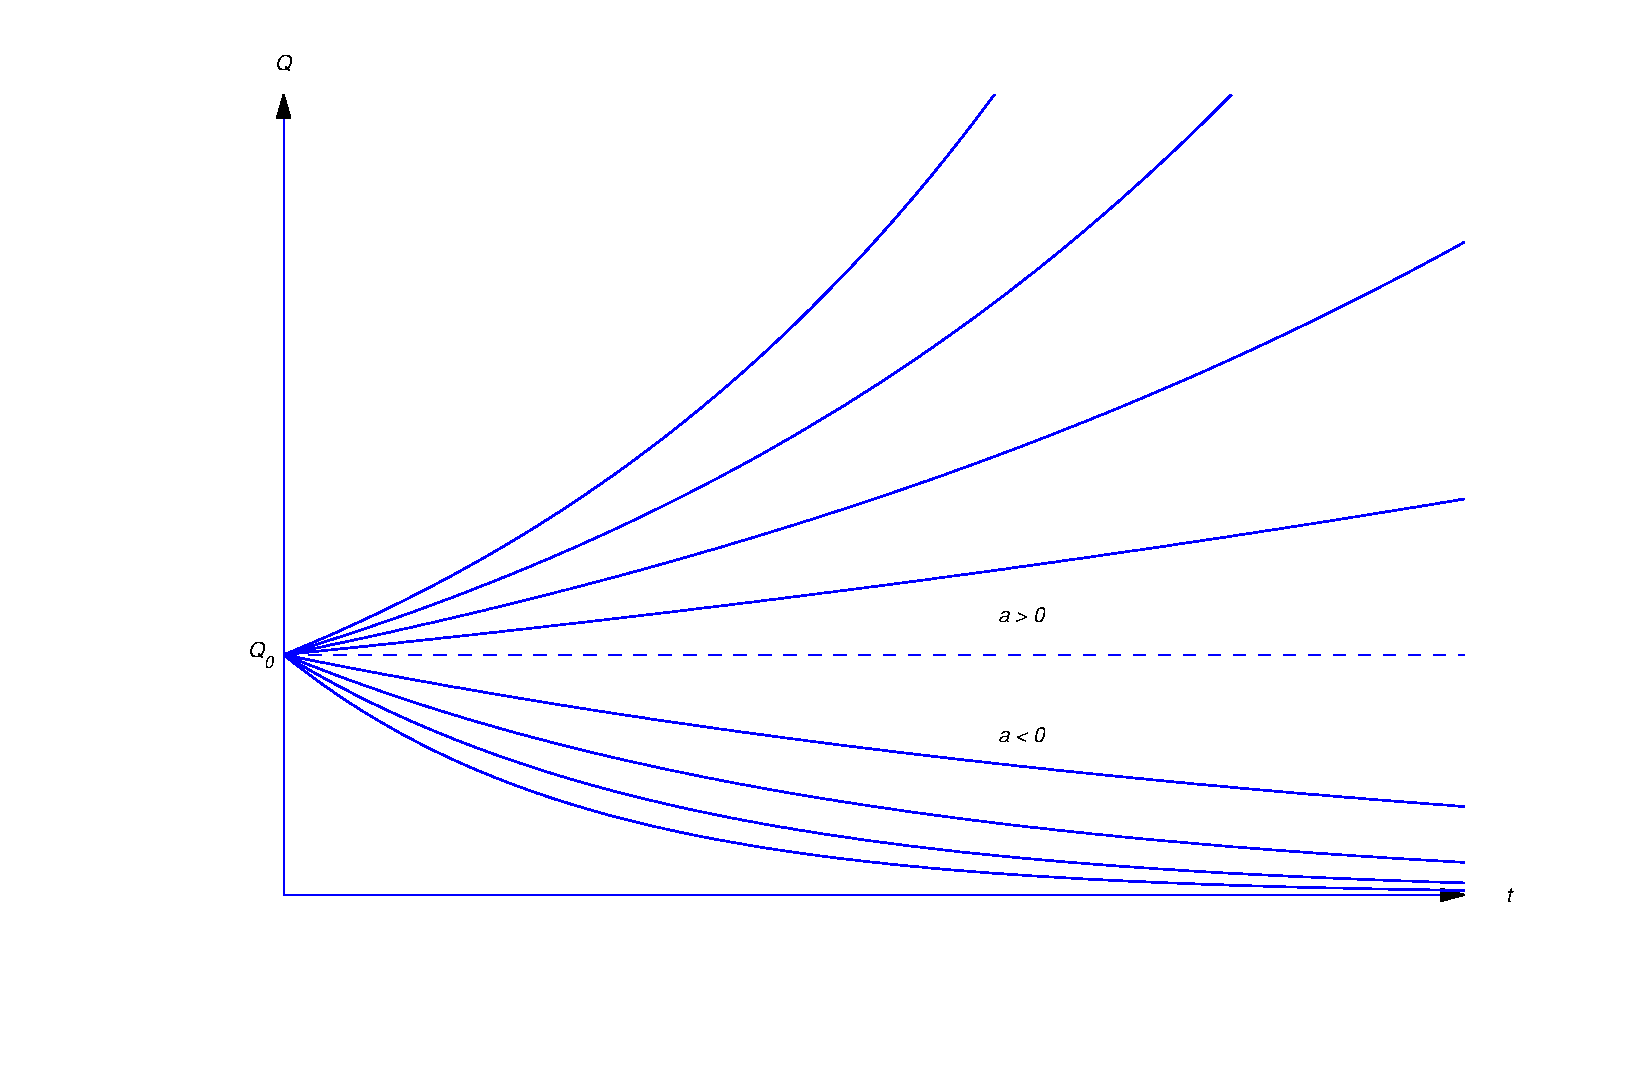
\includegraphics[bb=-78 148 689 643,width=5.67in,height=3.66in,keepaspectratio]{fig040101}
\color{blue}
\caption{\label{figure:4.1.1} Exponential growth  and decay}
  \label{figure4.1.1}
\end{figure}


\boxit{Radioactive Decay}


\noindent
Experimental evidence shows that radioactive material decays at a rate
proportional to the mass of the material present. According to this
model the mass $Q(t)$ of a radioactive material present at time $t$
satisfies \eqref{eq:4.1.1}, where $a$ is a negative constant whose value
for any given material must be determined by experimental observation.
For simplicity, we'll replace the negative constant $a$ by
$-k$, where
$k$ is a positive number that we'll call the {\color{blue}\it decay constant\/}
of the material. Thus, \eqref{eq:4.1.1} becomes
$$
Q'=-kQ.
$$
If the mass of the material present
at $t=t_0$ is $Q_0$,  the mass present at time $t$ is
 the solution of
$$
Q'=-kQ,\quad  Q(t_0)=Q_0.
$$
From \eqref{eq:4.1.2}  with $a=-k$, the solution of this initial value
problem is
\begin{equation} \label{eq:4.1.3}
Q=Q_0e^{-k(t-t_0)}.
\end{equation}

The {\color{blue}\it half--life} $\tau$ of a radioactive material is defined to be
the time required for half of its mass to decay; that is, if
$Q(t_0)=Q_0$, then \begin{equation} \label{eq:4.1.4} Q(\tau+t_0)={Q_0\over
2}.
\end{equation}
 From \eqref{eq:4.1.3} with $t=\tau+t_0$, \eqref{eq:4.1.4} is equivalent to
$$
Q_0e^{-k\tau}={Q_0\over 2},
$$
 so
$$
e^{-k\tau}={1\over 2}.
$$
 Taking logarithms  yields
$$
-k\tau=\ln{1\over 2}=-\ln2,
$$
 so the half-life is
\begin{equation} \label{eq:4.1.5}
\tau={1\over k}\ln2.
\end{equation}
(Figure \ref{figure:4.1.2}). The half-life is independent of $t_0$ and
$Q_0$, since it's determined by the properties of material, not by
the amount of the material present at any particular time.



\begin{figure}[tbp]
  \centering
  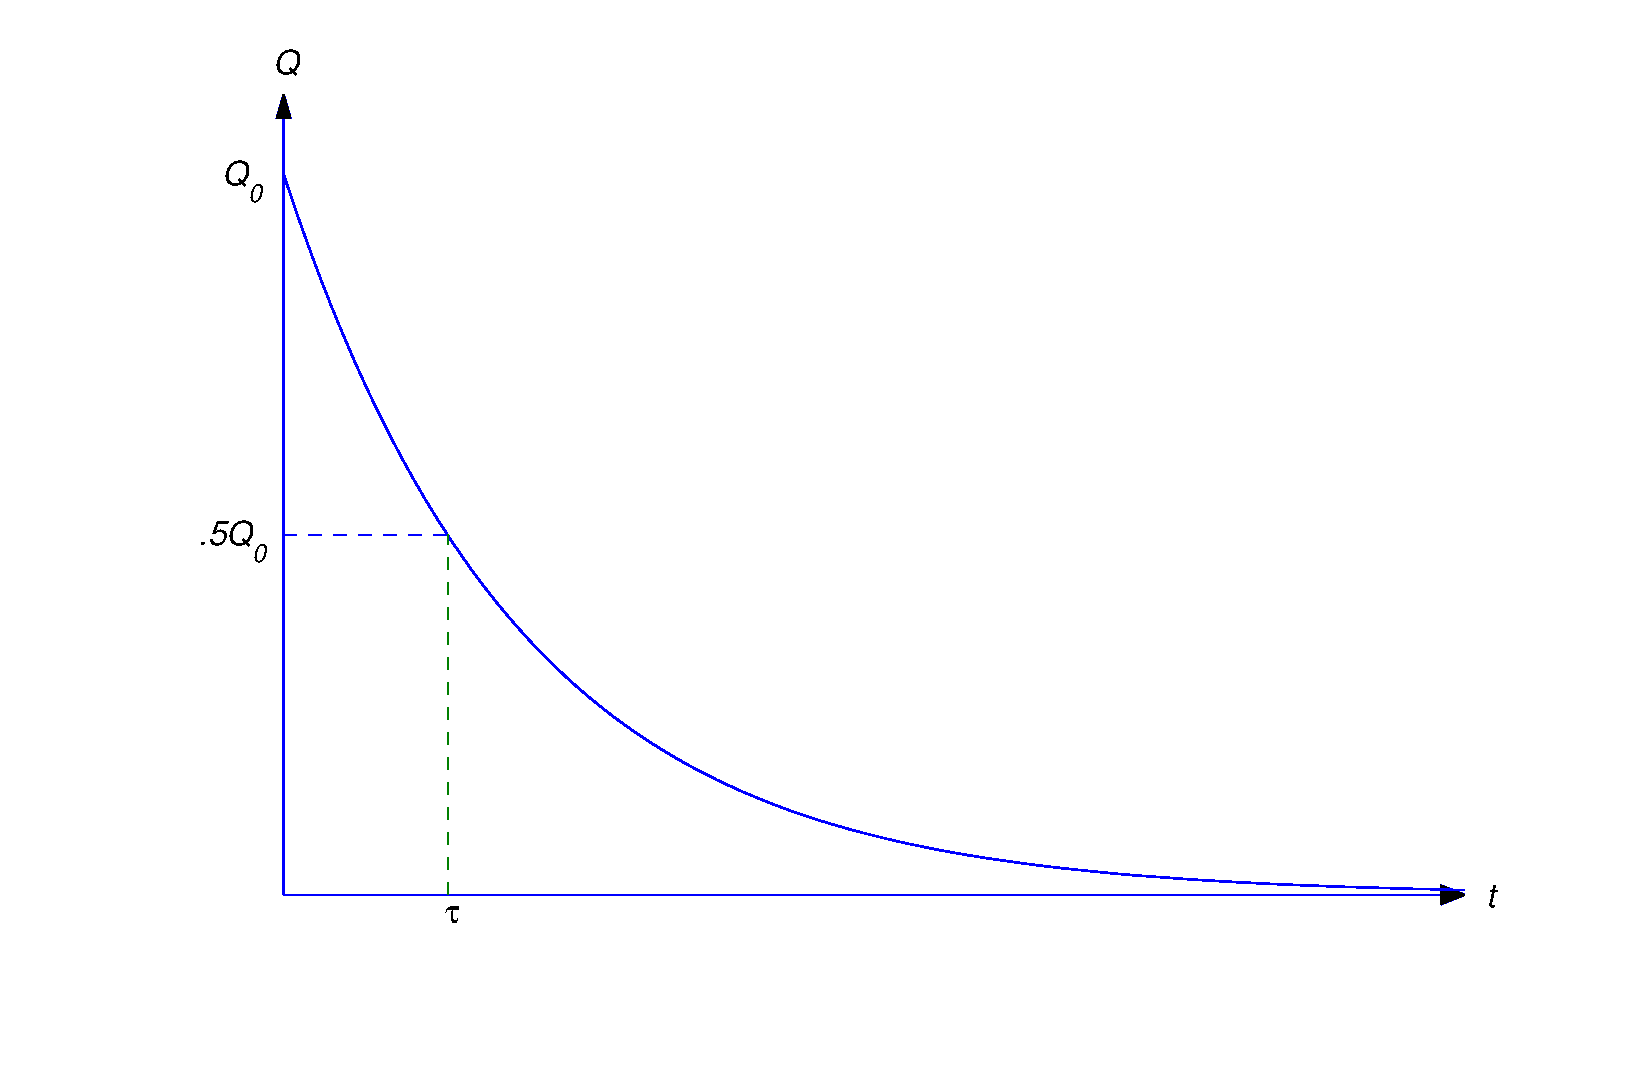
\includegraphics[bb=-78 148 689 643,width=5.67in,height=3.66in,keepaspectratio]{fig040102}
\color{blue}
\caption{Half-life of a radioactive substance}
  \label{figure:4.1.2}
\end{figure}

\begin{example}\label{example:4.1.1} \rm
A  radioactive substance has a half-life of 1620 years.
\begin{alist}
\item %(a)
If its mass is now 4 g (grams), how much will be left 810 years
from now?
\item % (b)
Find the time $t_1$ when 1.5 g of the substance remain.
\end{alist}
\end{example}

\solutionpart{a}  From \eqref{eq:4.1.3} with $t_0=0$ and
$Q_0=4$,
\begin{equation} \label{eq:4.1.6}
Q=4e^{-kt},
\end{equation}
 where we determine $k$ from \eqref{eq:4.1.5}, with $\tau$=
1620 years:
$$
k={\ln2\over\tau}={\ln2\over 1620}.
$$
 Substituting this in \eqref{eq:4.1.6} yields
\begin{equation} \label{eq:4.1.7}
Q=4e^{-(t\ln2)/1620}.
\end{equation}
 Therefore the mass left after 810 years will be
$$\begin{array}{rl}
Q(810) &=4e^{-(810\ln2)/1620}=4e^{-(\ln2)/2} \\
&=2\sqrt{2} \mbox{ g}.
\end{array}$$

\solutionpart{b}
 Setting $t=t_1$  in \eqref{eq:4.1.7} and requiring that
$Q(t_1)=1.5$ yields
$$
{3\over2}=4e^{(-t_1\ln2)/1620}.
$$
Dividing by 4 and taking logarithms yields
$$
\ln{3\over8}=-{t_1\ln2\over1620}.
$$
Since $\ln3/8=-\ln8/3$,
$$
t_1=1620{\ln8/3\over\ln2}\approx  2292.4\;\mbox{ years}.
$$

\boxit{Interest Compounded Continuously}


\noindent
Suppose we deposit an amount of money $Q_0$  in an
interest-bearing account and make no further deposits or withdrawals
for $t$ years, during which the account bears interest at a constant
annual rate $r$. To calculate the value of the account at the
end of $t$ years, we need one more piece of information: how the
interest is added to the account, or---as the bankers say---how it
is {\color{blue}\it compounded}. If the interest is compounded annually,  the
value of the account is multiplied by $1+r$ at the end of each year.
This means that after $t$ years the value of the account is
$$
Q(t)=Q_0(1+r)^t.
$$
If interest is compounded semiannually,  the
value of the account is multiplied by $(1+r/2)$ every 6 months.
Since this occurs twice annually, the value of the account after $t$
years is
$$
Q(t)=Q_0\left(1+{r\over 2}\right)^{2t}.
$$
In general, if interest is compounded $n$ times per year, the value of
the account is multiplied $n$ times per year by $(1+r/n)$;  therefore,
the value of the account
after $t$ years is
\begin{equation} \label{eq:4.1.8}
Q(t)=Q_0\left(1+{r\over n}\right)^{nt}.
\end{equation}
Thus, increasing the  frequency of  compounding increases the value of the
account after a fixed period of time. Table~\ref{table:4.1.1} shows the
effect
of increasing the number of compoundings over $t=5$ years on an initial
deposit of $Q_0=100$ (dollars), at an annual interest rate of 6\%.

\medskip

\begin{newtable} \label{table:4.1.1}
{Table \label{table:4.1.1} The effect of
compound interest}
\begin{center}
$$\begin{array}{|c|c|}\hline
n & \dst\$100 \left(1+{.06\over n}\right)^{5n}\\
\hbox{(number of compoundings} &   \hbox{(value in dollars}\\
\hbox{per year)} &\hbox{after 5 years)}\\
\hline
1 & \$133.82 \\
2 & \$134.39 \\
4 & \$134.68 \\
8 & \$134.83 \\
364 & \$134.98 \\\hline
\end{array}$$
\end{center}
\end{newtable}

\medskip
You can see from Table~\ref{table:4.1.1}  that the value of the account after 5
years is an increasing function of $n$. Now suppose  the maximum
allowable rate of interest on savings accounts is restricted by law,
but the time intervals between successive compoundings isn't ; then
competing banks can attract savers by compounding often. The ultimate
step in this direction is to {\color{blue}\it compound continuously}, by which we
mean that $n\to\infty$ in \eqref{eq:4.1.8}. Since we know from calculus
that
$$
\lim_{n\to\infty} \left(1+{r\over n}\right)^n=e^r,
$$
 this yields
$$\begin{array}{rl}
Q(t) & \dst=\lim_{n\to\infty} Q_0\left(1+{r\over
n}\right)^{nt}=Q_0 \left[
\lim_{n\to\infty} \left(1+{r\over n}\right)^n\right]^t \\[12pt]
&=Q_0e^{rt}.
\end{array}$$
Observe that $Q=Q_0e^{rt}$ is the solution of the initial value problem
$$
Q'=rQ, \quad Q(0)=Q_0;
$$
 that is, with continuous compounding the value of the account
grows exponentially.

\begin{example}\label{example:4.1.2} \rm
If \$150 is deposited in a bank that pays
$5{1\over2}$\% annual
interest compounded continuously,  the value of the account after
$t$ years is
$$
Q(t)=150e^{.055t}
$$
dollars. (Note that it's necessary to write the interest rate as a
decimal;   thus, $r=.055$.) Therefore, after $t=10$ years the value
of the account is
$$
Q(10)=150e^{.55} \approx \$259.99.
$$
\end{example}

\begin{example}\label{example:4.1.3} \rm
We wish to accumulate \$10,000 in 10 years by making a single deposit
in a savings account bearing $5{1\over2}$\% annual interest
compounded continuously. How much must we deposit in the account?
\end{example}

\solution  The value of the account at time $t$ is
\begin{equation} \label{eq:4.1.9}
Q(t)=Q_0e^{.055t}.
\end{equation}
Since we want $Q(10)$ to be \$10,000, the initial deposit $Q_0$ must
satisfy the equation
\begin{equation} \label{eq:4.1.10}
10000=Q_0e^{.55},
\end{equation}
 obtained by setting $t=10$ and $Q(10)=10000$ in
\eqref{eq:4.1.9}.  Solving \eqref{eq:4.1.10} for $Q_0$ yields
$$
Q_0=10000e^{-.55} \approx \$5769.50.
$$

\boxit{Mixed Growth and Decay}

\begin{example}\label{example:4.1.4} \rm
A radioactive substance with decay constant $k$ is produced at a
constant rate of $a$ units of mass per unit time.
\begin{alist}
\item %(a)
Assuming that $Q(0)=Q_0$, find the mass $Q(t)$ of the
substance present at time~$t$.

\item %(b)
Find $\lim_{t\to\infty} Q(t)$.
\end{alist}
\end{example}

\solutionpart{a}  Here
$$
Q'=\mbox{ rate of increase of } Q - \mbox{ rate of decrease
of } Q.
$$
The rate of increase is the constant $a$. Since $Q$ is radioactive
with decay constant $k$, the rate of decrease is $kQ$. Therefore
$$
Q'=a-kQ.
$$
This is a linear first order differential equation. Rewriting it and
imposing the initial condition shows that $Q$ is the solution of the
initial value problem
\begin{equation}  \label{eq:4.1.11}
Q'+kQ=a, \quad Q(0)=Q_0.
\end{equation}
Since
$e^{-kt}$ is a solution of the complementary equation, the solutions
of \eqref{eq:4.1.11} are of the form $Q=ue^{-kt}$, where $u'e^{-kt}=a$, so
$u'=ae^{kt}$. Hence,
$$
u={a\over k}e^{kt}+c
$$
and
$$
Q=ue^{-kt}={a\over k}+ce^{-kt}.
$$
 Since $Q(0)=Q_0$, setting $t=0$ here yields
$$
Q_0={a\over k}+c  \mbox{\quad or \quad} c=Q_0-{a\over k}.
$$
 Therefore
\begin{equation} \label{eq:4.1.12}
Q={a\over k}+\left(Q_0-{a\over k}\right)e^{-kt}.
\end{equation}

\solutionpart{b}
Since $k > 0$,  $\lim_{t\to\infty} e^{-kt}=0$, so
from \eqref{eq:4.1.12}
$$
\lim_{t\to\infty} Q(t)={a\over k}.
$$
This limit depends only on $a$ and $k$, and not on $Q_0$.
We say that $a/k$ is the {\color{blue}\it steady state} value of $Q$. From
\eqref{eq:4.1.12} we also see that $Q$ approaches its steady state value
from above if $Q_0 > a/k$, or from below if $Q_0 < a/k$. If $Q_0=a/k$,
then $Q$ remains constant (Figure \ref{figure:4.1.3}).


\begin{figure}[tbp]
  \centering
  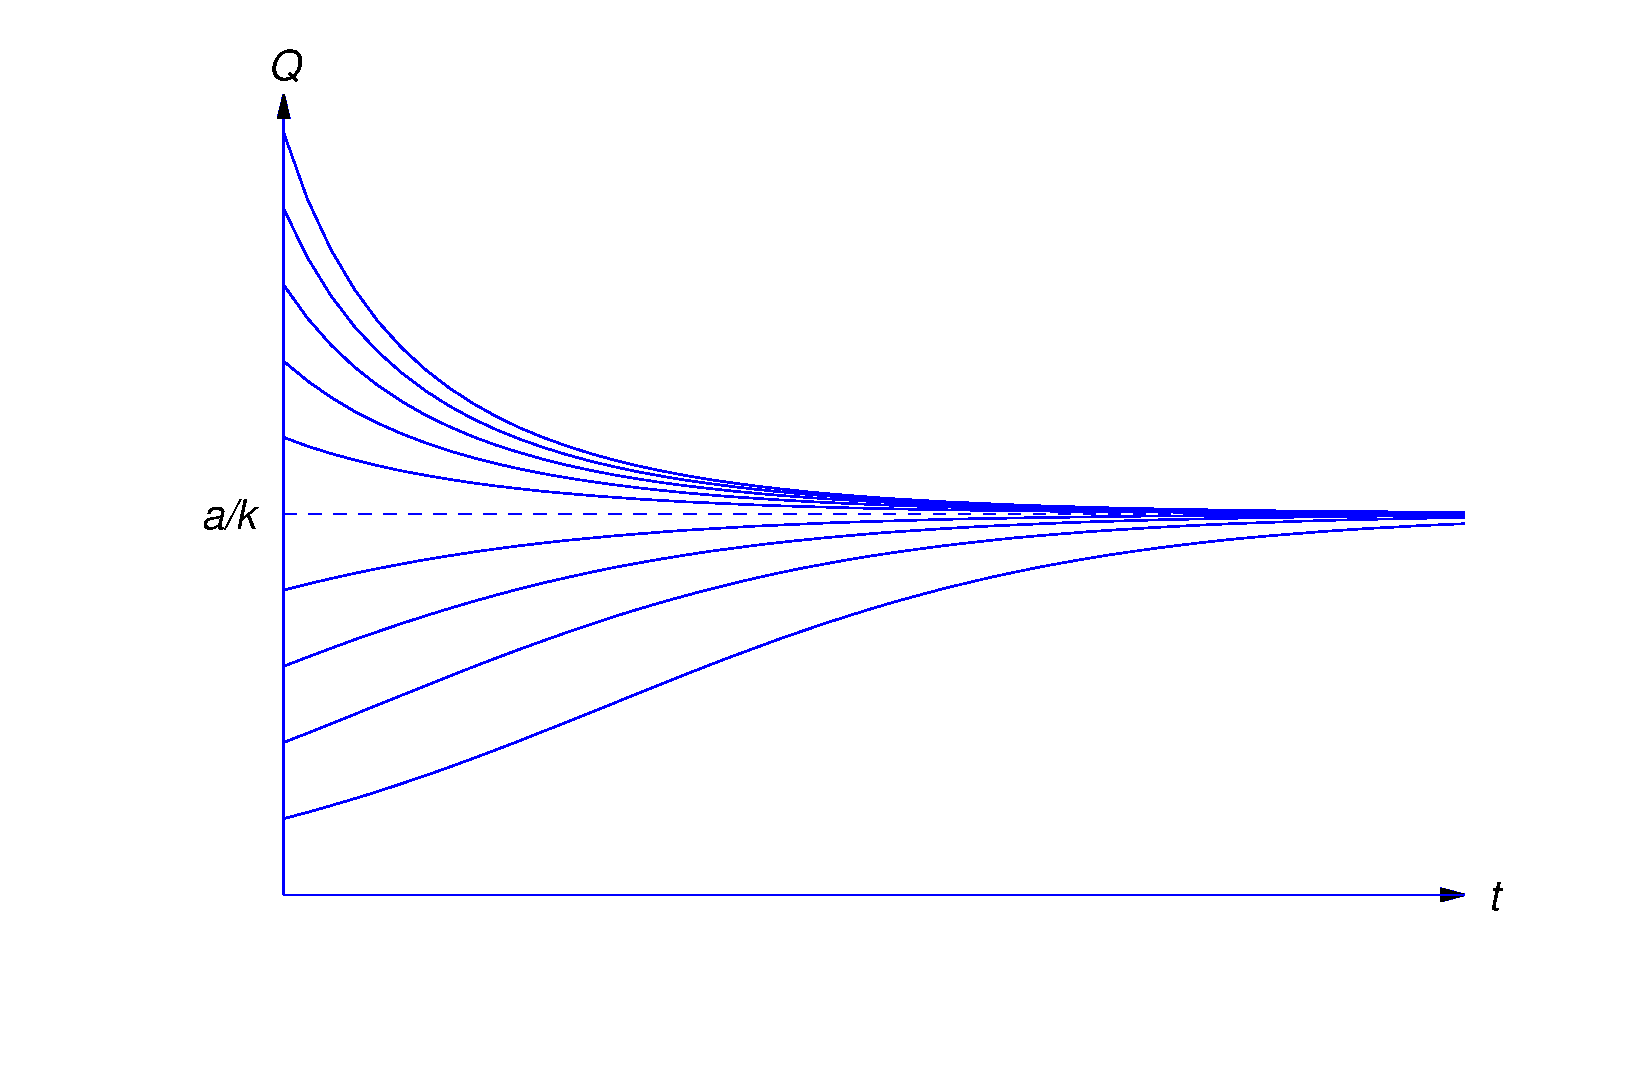
\includegraphics[bb=-78 148 689 643,width=5.67in,height=3.66in,keepaspectratio]{fig040103}
\color{blue}
\caption{$Q(t)$ approaches the steady state value
$\dst{a\over k}$ as $t\to\infty$}
  \label{figure:4.1.3}
\end{figure}




\boxit{Carbon Dating}


\noindent
The fact that $Q$ approaches a steady state value in the
situation discussed in Example 4 underlies the method of {\color{blue}\it carbon
dating}, devised by  the American chemist  and Nobel Prize Winner
\href{http://www.nobelprize.org/nobel_prizes/chemistry/laureates/1960/libby-lecture.pdf}
{\color{blue}\it W.S. Libby}.

Carbon 12 is stable, but carbon-14, which is produced by cosmic
bombardment of nitrogen in the upper atmosphere, is radioactive with a
half-life of about 5570 years. Libby assumed that the
quantity
of carbon-12 in the atmosphere has been constant throughout time, and
that the quantity of radioactive carbon-14 achieved its steady state
value long ago as a result of its creation and decomposition over
millions of years. These assumptions led Libby to conclude that the
ratio of carbon-14 to carbon-12 has been nearly constant for a long
time. This constant, which we denote by $R$, has been determined
experimentally.

Living cells absorb both carbon-12 and carbon-14 in the proportion in
which they are present in the environment. Therefore the ratio of
carbon-14 to carbon-12 in a living cell is always $R$. However, when
the cell dies it ceases to absorb carbon, and the ratio of carbon-14
to carbon-12 decreases exponentially as the radioactive carbon-14
decays. This is the basis for the method of carbon dating, as
illustrated in the next example.

\begin{example}\label{example:4.1.5} \rm
An archaeologist investigating the site of an ancient village finds a
burial ground where the amount of carbon-14 present in individual
remains is between 42 and 44\% of the amount present in live
individuals. Estimate the age of the village and the length of time
for which it survived.
\end{example}

\solution Let $Q=Q(t)$ be the quantity of carbon-14 in an individual
set of remains $t$ years after death, and let $Q_0$ be the quantity
that would be present in  live individuals.
Since carbon-14 decays exponentially with half-life 5570 years, its
decay constant is
$$
k={\ln2\over 5570}.
$$
 Therefore
$$
Q=Q_0e^{-t(\ln2)/5570}
$$
 if we choose our time scale so that $t_0=0$ is the
time of death.  If we know the present value of $Q$  we
can solve this equation for $t$, the number of years since
death occurred.  This yields
$$
t=-5570 {\ln Q/Q_0\over\ln2}.
$$
It is given that $Q=.42Q_0$ in the remains of individuals who died
first. Therefore these deaths occurred about
$$
t_1=-5570 {\ln .42\over\ln2} \approx 6971
$$
 years ago.  For the most recent deaths, $Q=.44
Q_0$; hence, these deaths occurred about
$$
t_2=-5570 {\ln .44\over\ln2} \approx 6597
$$
 years ago.  Therefore it's reasonable to conclude
that the village was founded about 7000 years ago,
and lasted for about 400 years.

\boxit{A Savings Program}

\vspace*{-.2in}
\noindent
\begin{example}\label{example:4.1.6} \rm
A person opens a savings account with an initial deposit of \$1000 and
subsequently deposits \$50 per week. Find the value $Q(t)$ of the
account at time $t > 0$, assuming that the bank pays 6\%
interest compounded continuously.
\end{example}

\solution Observe that $Q$ isn't  continuous, since there are 52
discrete deposits per year of \$50 each. To construct a mathematical
model for this problem in the form of a differential equation, we make
the simplifying assumption that the deposits are made continuously at
a rate of \$2600 per year. This is essential, since solutions of
differential equations are continuous functions. With this assumption,
$Q$ increases continuously at the rate
$$
Q'=2600+.06 Q
$$
and therefore $Q$ satisfies the differential equation
\begin{equation} \label{eq:4.1.13}
Q'-.06Q=2600.
\end{equation}
(Of course, we must recognize that the solution of this equation
is an approximation to the true value of $Q$ at any given time. We'll
discuss this further below.)  Since $e^{.06t}$ is a solution of the
complementary equation, the solutions of \eqref{eq:4.1.13}  are of the
form   $Q=ue^{.06t}$,  where $u'e^{.06t}=2600$. Hence,
$u'=2600e^{-.06t}$,
$$
u=- {2600\over .06}e^{-.06t}+c
$$
and
\begin{equation} \label{eq:4.1.14}
Q=ue^{.06t}=-{2600\over .06}+ce^{.06t}.
\end{equation}
 Setting $t=0$ and $Q=1000$ here yields
$$
c=1000+{2600\over .06},
$$
and substituting this into \eqref{eq:4.1.14} yields
\begin{equation} \label{eq:4.1.15}
Q=1000e^{.06t}+{2600\over .06}(e^{.06t}-1),%\tag15
\end{equation}
where the first term is the value due to the initial deposit and the
second is due to the subsequent weekly deposits. \bbox

Mathematical models must be tested for validity by comparing
predictions based on them with the actual outcome of experiments.
Example 6 is unusual in that we can compute the exact value of the
account at any specified time and compare it with the approximate
value predicted by \eqref{eq:4.1.15} (See Exercise \ref{exer:4.1.21}.). The
follwing table
 gives a comparison for a ten year period. Each exact answer
corresponds to the time of the year-end deposit, and each year is
assumed to have exactly 52 weeks.

$$
\vbox{\tabskip=0pt \offinterlineskip
\def\tablerule{\noalign{\hrule}}
\halign{\hfill#\hfill&\qquad\hfill#\hfill&\qquad\hfill#\hfill
  &\qquad\hfill#\hfill&\qquad#\hfill\cr
%\noalign{\centerline{\bf Table \label{table:4.1.2}}}
\noalign{\vskip12pt}
%\noalign{\centerline{Value of the Saver's Account (Example
%\ref{example:4.1.6})}}
\noalign{\vskip22pt}
Year & Approximate Value of $Q$ & Exact Value of  $P$ & Error & Percentage
Error
\cr & (Example~\ref{example:4.1.6}) & (Exercise~\ref{exer:4.1.21}) & $Q-P$ &\ \;
$(Q-P)/P$ \cr \noalign{\vskip16pt}
\  1 & \$ 3741.42 & \$ 3739.87 & \$ 1.55 &\ \; $.0413 $\% \cr
\noalign{\vskip7pt}
\  2 &\  \, 6652.36 &\ \;  6649.17 &\ \; 3.19 &\ \; $.0479$
\cr
\noalign{\vskip7pt}
\  3 &\  \, 9743.30 &\ \;  9738.37 &\ \; 4.93 &\ \; $.0506$
\cr
\noalign{\vskip7pt}
\  4 & \, 13,025.38 & \, 13,018.60 &\ \; 6.78 &\ \; $.0521$
\cr
\noalign{\vskip7pt}
\  5 & \, 16,510.41 & \, 16,501.66 &\ \; 8.75 &\ \; $.0530 $
\cr
\noalign{\vskip7pt}
\  6 & \, 20,210.94 & \, 20,200.11 & 10.83 &\ \; $.0536$
\cr
\noalign{\vskip7pt}
\  7 & \, 24,140.30 & \, 24,127.25 & 13.05 &\ \; $.0541 $
\cr
\noalign{\vskip7pt}
\  8 & \, 28,312.63 & \, 28,297.23 & 15.40 &\ \; $.0544 $
\cr
\noalign{\vskip7pt}
\  9 & \, 32,742.97 & \, 32,725.07 & 17.90 &\ \; $.0547 $
\cr
\noalign{\vskip7pt}
10 & \, 37,447.27 & \, 37,426.72 & 20.55 &\ \; $.0549 $ \cr}}
$$
\newpage

\exercises

\begin{exerciselist}
\item\label{exer:4.1.1}
The half-life of a radioactive substance is 3200
years.  Find the quantity $Q(t)$ of the substance left at
time $t > 0$ if $Q(0)=20$ g.

\item\label{exer:4.1.2}
The half-life of a radioactive substance is 2 days.  Find
the time required for a given amount of the material to
decay to 1/10 of its original mass.

\item\label{exer:4.1.3}
A  radioactive material loses 25\% of its mass
in 10 minutes.  What is its half-life?

\item\label{exer:4.1.4}
A  tree contains a known percentage $p_0$ of
a radioactive substance with half-life $\tau$.  When the
tree dies the substance decays and isn't  replaced.  If the
percentage of the substance in the fossilized remains of
such a tree is found to be $p_1$, how long has the tree been
dead?

\item\label{exer:4.1.5}
If $t_p$ and $t_q$ are the times required for a radioactive
material to decay to $1/p$ and $1/q$  times
its original mass (respectively), how are $t_p$ and $t_q$ related?

\item\label{exer:4.1.6}
Find the decay constant $k$ for a radioactive substance,
given that the mass of the substance is $Q_1$ at time $t_1$
and $Q_2$ at time $t_2$.

\item\label{exer:4.1.7}
A process creates a radioactive substance at the rate of 2
g/hr and the substance decays at a rate proportional to
its mass, with constant of proportionality
$k=.1 (\mbox{hr})^{-1}$.  If $Q(t)$ is the mass of the
substance at time $t$, find $\lim_{t\to\infty}Q(t)$.

\item\label{exer:4.1.8}
A bank pays interest continuously at the rate of 6\%.
How long does it take for a deposit of $Q_0$ to grow in
value to $2Q_0$?

\item\label{exer:4.1.9}
At what rate of interest, compounded continuously, will a
bank deposit double in value in 8 years?

\item\label{exer:4.1.10}
A savings account pays 5\% per annum interest compounded
continuously. The initial deposit is $Q_0$ dollars. Assume that there
are no subsequent withdrawals or deposits.
\begin{alist}
\item % (a)
How long will it take for the value of the account to triple?
\item % (b)
What is $Q_0$ if the value of the account after 10 years is \$100,000
dollars?
\end{alist}

\item\label{exer:4.1.11}
A candymaker makes 500 pounds of candy per week, while
his large family eats the candy at a rate equal to $Q(t)/10$
pounds per week, where $Q(t)$ is the amount of candy present
at time $t$.
\begin{alist}
\item %(a)
Find $Q(t)$ for $t > 0$ if the candymaker has 250 pounds of
candy at $t=0$.
\item %(b)
Find $\lim_{t\to\infty} Q(t)$.
\end{alist}

\item\label{exer:4.1.12}
Suppose a substance decays at a yearly rate  equal
to half the square of the mass of the substance present.  If
we start with 50 g of the substance, how long will it be
until only 25 g remain?

\item\label{exer:4.1.13}
A super bread dough increases in volume at a rate
proportional to the volume $V$ present.  If $V$ increases by
a factor of 10 in 2 hours and $V(0)=V_0$, find $V$ at any
time $t$.  How long will it take for $V$ to increase to $100
V_0$?

\item\label{exer:4.1.14}
A radioactive substance decays at a rate proportional to the
amount present, and half the original quantity $Q_0$ is left
after 1500 years. In how many years would the original
amount be reduced to $3Q_0/4$?  How much will be
left after 2000 years?


\item\label{exer:4.1.15}
A wizard creates gold continuously at the rate of 1 ounce
per hour, but an assistant steals it continuously at the
rate of 5\% of however much  is there per hour.  Let $W(t)$
be the number of ounces that the wizard has at time $t$.
Find $W(t)$ and $\lim_{t\to\infty}W(t)$ if  $W(0)=1$.

\item\label{exer:4.1.16}
A process creates a radioactive substance at the rate of 1
g/hr, and the substance decays at an hourly rate
 equal to 1/10 of the mass present (expressed in
grams).  Assuming that there are initially 20 g, find
the mass $S(t)$ of the substance present at time $t$, and
find $\lim_{t\to\infty} S(t)$.

\item\label{exer:4.1.17}
A tank is empty at $t=0$.  Water is added to the tank at
the rate of 10 gal/min, but it leaks out at a rate
 (in gallons per minute)  equal to the number of
gallons in the tank.  What is the smallest capacity the tank
can have if this process is to continue forever?

\item\label{exer:4.1.18}
A person deposits \$25,000 in a bank that pays 5\% per
year interest, compounded continuously.  The person
continuously withdraws from the account at the rate of \$750
per year.  Find $V(t)$, the value of the account at time $t$
after the initial deposit.

\item\label{exer:4.1.19}
  A person has a fortune that grows at rate proportional to the
square root of its worth. Find the  worth $W$ of the fortune as a function
of $t$ if it was  \$1 million 6 months ago and
is \$4 million today.

\item\label{exer:4.1.20}
Let $p=p(t)$ be the quantity of a  product present at
time $t$. The product is manufactured continuously at a
rate proportional to $p$, with proportionality constant 1/2,
and it's consumed continuously at a rate proportional to
$p^2$, with proportionality constant 1/8.  Find $p(t)$ if
$p(0)=100$.

\item\label{exer:4.1.21}

\begin{alist}
\item % (a)
 In the situation of Example~\ref{example:4.1.6}
find the exact value $P(t)$ of the person's account after $t$
years, where $t$ is an integer.  Assume that each year has
exactly 52 weeks, and include the year-end
deposit in the computation.

\hint{At time $t$ the initial $\$1000$
has been on deposit for $t$ years.  There have been $52t$
deposits of $\$50$ each.  The first $\$50$ has been on deposit
for $t-1/52$ years, the second for $t-2/52$ years $\cdots$
in general, the $j$th $\$50$ has been on deposit for $t-j/52$
years $(1 \le j \le 52t)$.  Find the present value of each
$\$50$ deposit assuming $6$\% interest compounded
continuously, and use the formula
$$
1+x+x^2+\cdots+x^n={1-x^{n+1}\over 1-x}\
(x \ne 1)
$$
to find their total value.}

\item % (b)
 Let
$$
p(t)={Q(t)-P(t)\over P(t)}
$$
be the relative error after $t$ years.  Find
$$
p(\infty)=\lim_{t\to\infty}p(t).
$$
\end{alist}

\item\label{exer:4.1.22}
A homebuyer borrows $P_0$ dollars at an annual interest rate $r$,
agreeing to repay the loan with equal monthly payments of $M$ dollars
per month over $N$ years.
\begin{alist} \item % (a)
Derive a
differential equation for the loan principal (amount that the
homebuyer owes) $P(t)$ at time $t>0$, making the simplifying
assumption that the homebuyer repays the loan continuously rather than
in discrete steps. (See Example~\ref{example:4.1.6} .)

\item %(b)
Solve the equation derived in \part{a}.

\item % (c)
 Use the result of \part{b} to determine an approximate
value for $M$  assuming that each year has exactly 12 months of
equal length.

\item % (d)
 It can be shown that the exact value of $M$  is given by
$$
M={rP_0\over 12}\left(1-(1+r/12)^{-12N}\right)^{-1}.
$$
Compare    the value of $M$ obtained from the answer in \part{c} to the
exact value  if
 (i) $P_0=\$50,000$, $r=7{1\over2}$\%, $N=20$
 (ii) $P_0=\$150,000$, $r=9.0$\%, $N=30$.
\end{alist}

\item\label{exer:4.1.23}
Assume that the homebuyer of Exercise \ref{exer:4.1.22} elects to repay the
loan continuously at the rate of $\alpha M$ dollars per month,
where $\alpha$ is a constant greater than 1. (This is called {\color{blue}\it
accelerated payment\/}.)
\begin{alist}
\item % (a)
 Determine the time $T(\alpha)$ when the loan
will be paid off and the amount $S(\alpha)$ that the homebuyer will save.

\item % (b)
 Suppose $P_0=\$50,000$, $r=8$\%, and $N=15$.
Compute
the savings realized by accelerated payments with $\alpha=1.05,1.10$, and
$1.15$.
\end{alist}

\item\label{exer:4.1.24} A benefactor wishes to establish a trust fund to
pay a researcher's salary for $T$ years. The salary is to start at
$S_0$ dollars per year and increase at a fractional rate of $a$ per
year. Find the amount of money $P_0$ that the benefactor must deposit
in a trust fund paying interest at a rate $r$ per year. Assume that
the researcher's salary is paid continuously, the interest is
compounded continuously, and the salary increases are granted
continuously.

\item\label{exer:4.1.25} \Lex
A radioactive substance with decay constant $k$ is produced
at the rate of
$$
{at\over1+btQ(t)}
$$
 units of mass per unit time, where
$a$ and $b$ are positive constants and $Q(t)$ is the mass of the
substance present at time $t$;   thus, the rate of production is small
at the start
 and tends to slow when $Q$ is large.
\begin{alist}
\item % (a)
Set up a differential equation for $Q$.
\item % (b)
Choose your own positive values for $a$, $b$, $k$, and
$Q_0=Q(0)$.
Use a numerical method
to discover what happens to $Q(t)$
as $t\to\infty$. (Be precise, expressing your conclusions in terms of
$a$, $b$, $k$. However,  no proof is required.)
\end{alist}


\item\label{exer:4.1.26} \Lex
Follow the instructions of Exercise~\ref{exer:4.1.25}, assuming that
the substance is produced at the rate of   $at/(1+bt(Q(t))^2)$
units of mass per unit of time.


\item\label{exer:4.1.27} \Lex
Follow the instructions of Exercise~\ref{exer:4.1.25}, assuming that
the substance is produced at the rate of   $at/(1+bt)$
units of mass per unit of time.


\end{exerciselist}


\newsection{2}{Applications of First Order Equations} {Cooling and Mixing}
\currentpdfbookmark{Section 4.2 Cooling and Mixing}{section:4.2}
\vskip14pt
\renewcommand{\thissection}{\sectiontitle{\,
COOLING AND MIXING}}
\thissection


\boxit{Newton's Law of Cooling}


\noindent
Newton's law of cooling states that if an object with temperature
$T(t)$ at time $t$ is in a medium with temperature $T_m(t)$,  the
rate of change of $T$ at time $t$ is proportional to $T(t)-T_m(t)$;
thus,
$T$ satisfies a differential equation of the form
\begin{equation} \label{eq:4.2.1}
T'=-k(T-T_m).
\end{equation}
 Here $k > 0$, since the temperature of the object must decrease if
$T > T_m$, or increase if $T < T_m$.  We'll call $k$  the {\color{blue}\it
temperature decay constant of the medium\/}.

For simplicity, in this section we'll assume  that the medium is
maintained at a constant temperature $T_m$. This is another example of
 building a simple mathematical model for a physical
phenomenon. Like most mathematical models it has its limitations. For
example, it's reasonable to assume that the temperature of a room
remains approximately constant if the cooling object is a cup of
coffee, but perhaps not if it's a huge cauldron of molten metal. (For
more on this see Exercise~\ref{exer:4.2.17}.)


To solve  \eqref{eq:4.2.1}, we rewrite it as
$$
T'+kT=kT_m.
$$
Since $e^{-kt}$ is a solution of the complementary equation, the
solutions of this equation are of the form $T=ue^{-kt}$, where
$u'e^{-kt}=kT_m$, so $u'=kT_me^{kt}$. Hence,
$$
u=T_me^{kt}+c,
$$
so
$$
T=ue^{-kt}=T_m+ce^{-kt}.
$$
If $T(0)=T_0$,  setting $t=0$ here yields $c=T_0-T_m$, so
\begin{equation} \label{eq:4.2.2}
T=T_m+(T_0-T_m)e^{-kt}.
\end{equation}
Note that $T-T_m$ decays exponentially, with decay constant $k$.


\begin{example}\label{example:4.2.1}\rm
A ceramic insulator is baked at $400^\circ$C and cooled in a room in
which the temperature is $25^\circ$C. After 4 minutes the
temperature of the insulator is $200^\circ$C. What is its temperature
after 8 minutes?
\end{example}

\solution Here $T_0=400$ and $T_m=25$, so \eqref{eq:4.2.2} becomes
\begin{equation} \label{eq:4.2.3}
T=25+375e^{-kt}.
\end{equation}
 We determine $k$ from the stated condition that  $T(4)=200$;
that is,
$$
200=25+375e^{-4k};
$$
 hence,
$$
e^{-4k} = {175\over 375} = {7\over 15}.
$$
 Taking logarithms and solving for $k$ yields
$$
k=-{1\over 4} \ln {7\over 15}={1\over 4}\ln {15\over 7}.
$$
 Substituting this into \eqref{eq:4.2.3} yields
$$
T=25+375 e^{-{t\over 4} \ln {15\over 7}}
$$
(Figure~\ref{figure:4.2.1}).
Therefore the temperature of the insulator after
8 minutes is
$$\begin{array}{rl}
T(8) & \dst = 25+375 e^{-2 \ln {15\over 7}} \\[9pt]
& \dst = 25+375 \left({7\over 15}\right)^2 \approx
107^\circ \mbox{C}.
\end{array}$$






\begin{figure}[tbp]
  \centering
  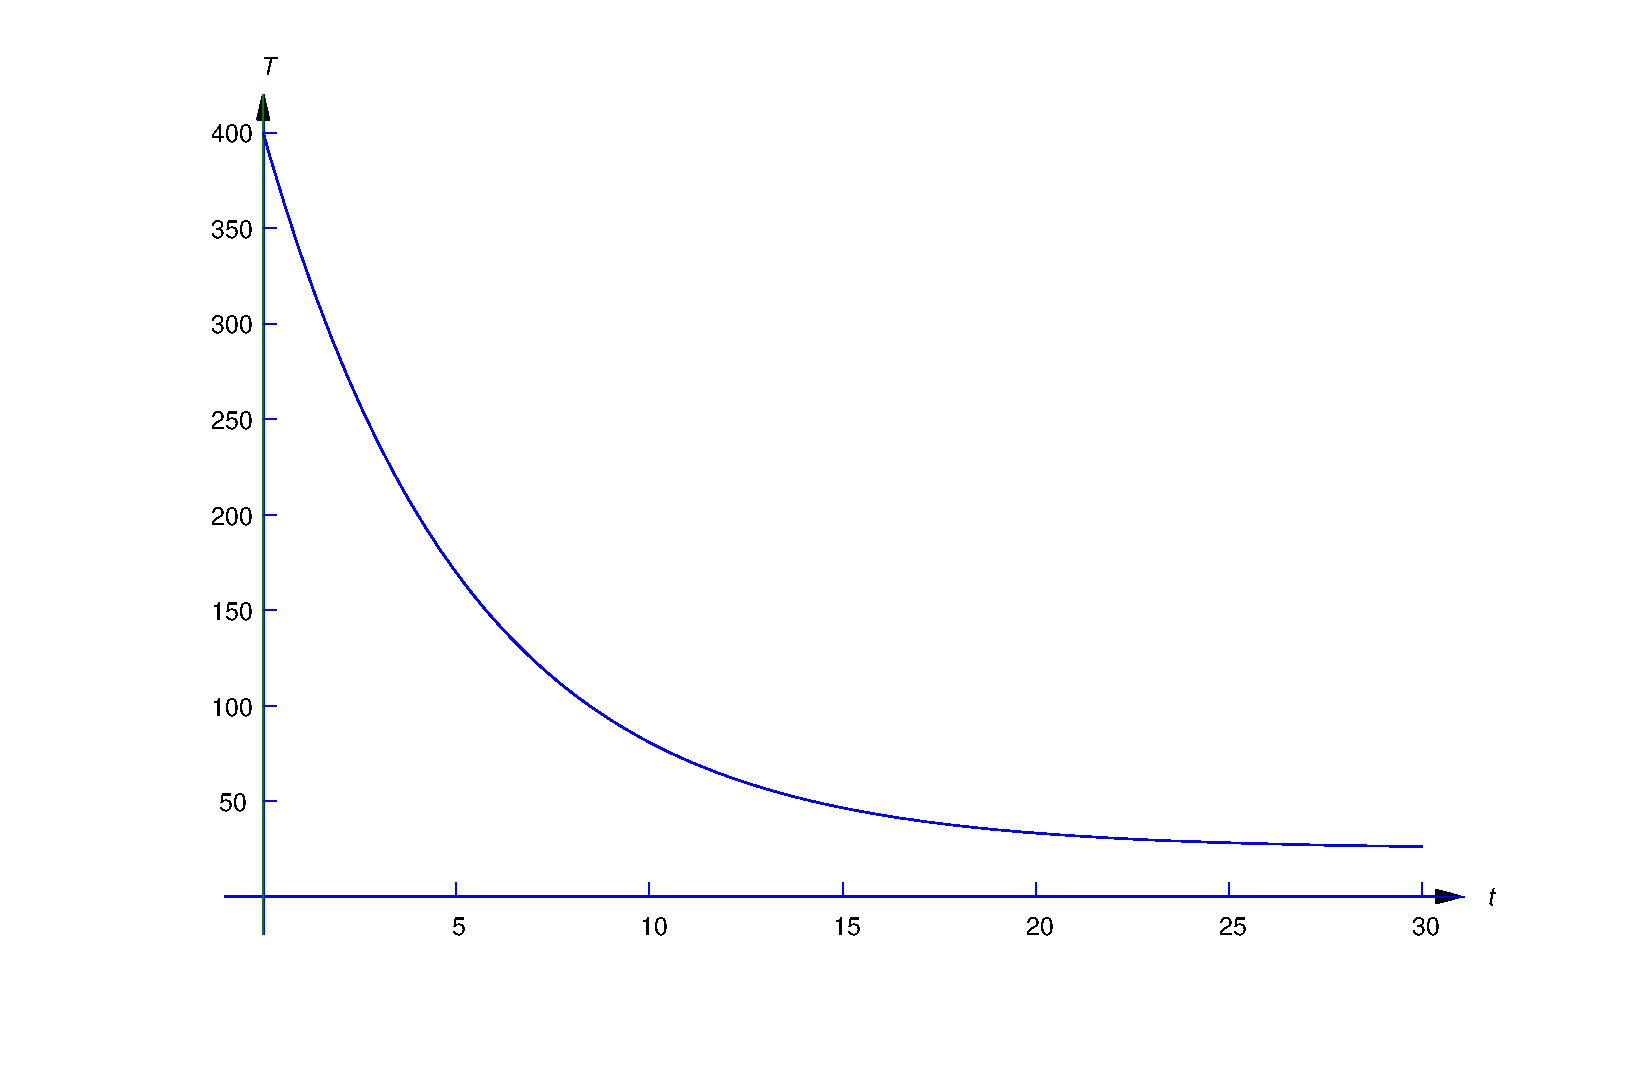
\includegraphics[bb=-78 148 689 643,width=5.67in,height=3.66in,keepaspectratio]{fig040201}
\color{blue}
\caption{$T=25+375e^{-(t/4)\ln 15/7}$}
  \label{figure:4.2.1}
\end{figure}

\begin{example}\label{example:4.2.2}\rm
An object with temperature $72^\circ$F is placed outside, where the
temperature is $-20^\circ$F. At 11:05 the temperature of the object
is $60^\circ$F and at 11:07 its temperature is $50^\circ$F. At what
time was the object placed outside?
\end{example}

\solution Let $T(t)$ be the temperature of the object at time $t$. For
convenience, we choose the origin $t_0=0$ of the time scale to be
11:05 so that $T_0=60$. We must determine the time $\tau$ when
$T(\tau)=72$. Substituting $T_0=60$ and $T_m=-20$ into \eqref{eq:4.2.2}
yields
$$
T  = -20+\bigl(60-(-20)\bigr)e^{-kt}
$$
 or
\begin{equation} \label{eq:4.2.4}
T = -20+80e^{-kt}.
\end{equation}
We obtain $k$ from the stated condition that the temperature of the
object is 50$^\circ$F at 11:07. Since 11:07 is $t=2$ on our time
scale, we can determine $k$ by substituting $T=50$ and $t=2$ into
\eqref{eq:4.2.4} to obtain
$$
50 = -20+80e^{-2k}
$$
(Figure~\ref{figure:4.2.2});
 hence,
$$
e^{-2k}={70\over 80}={7\over 8}.
$$
 Taking logarithms and solving for $k$ yields
$$
k =-{1\over 2} \ln {7\over 8} = {1\over 2} \ln {8\over 7}.
$$
 Substituting this into \eqref{eq:4.2.4} yields
$$
T = -20+80 e^{-{t\over 2}\ln {8\over 7}},
$$
 and the condition $T(\tau)=72$  implies that
$$
72 =-20+80 e^{-{\tau\over 2} \ln {8\over 7}};
$$
 hence,
$$
e^{-{\tau\over 2} \ln {8\over 7}} ={92\over 80} =
{23\over 20}.
$$
Taking logarithms and solving for $\tau$ yields
$$
\tau = -{2 \ln {23\over 20}\over \ln {8\over 7}} \approx-2.09\
\mbox{min}.
$$
Therefore the object was placed outside
about 2 minutes and 5 seconds before 11:05; that is,
at 11:02:55.


\begin{figure}[tbp]
  \centering
  \includegraphics[bb=-78 148 689 643,width=5.67in,height=3.66in,keepaspectratio]{fig040202}
\color{blue}
  \caption{$T = -20+80 e^{-{t\over 2}\ln {8\over 7}}$}
  \label{figure:4.2.2}
\end{figure}




\boxit{Mixing Problems}


\noindent
In the next two examples a saltwater solution with a given
concentration (weight of salt per unit volume of solution) is added at
a specified rate to a tank that initially contains saltwater with a
different concentration. The problem is to determine the quantity of
salt in the tank as a function of time. This is an example of a {\color{blue}\it
mixing problem\/}. To construct a tractable mathematical model for
mixing problems we assume in our examples (and most exercises) that
the mixture is stirred instantly so that the salt is always uniformly
distributed throughout the mixture. Exercises~\ref{exer:4.2.22}
and \ref{exer:4.2.23} deal with situations where this isn't  so, but
the distribution of salt becomes approximately uniform as
$t\to\infty$.

\begin{example}\label{example:4.2.3}  \rm
A tank initially contains 40 pounds of salt dissolved in 600 gallons
of water. Starting at $t_0 = 0$, water that contains 1/2 pound of salt
per gallon is poured into the tank at the rate of 4 gal/min and the
mixture is drained from the tank at the same rate
(Figure~\ref{figure:4.2.3}).
\begin{alist}
\item % (a)
Find a differential equation for the quantity $Q(t)$ of salt in the
tank at time $t > 0$, and solve the equation to determine $Q(t)$.
\item % (b)
 Find $\lim_{t\to\infty}Q(t)$.
\end{alist}
\end{example}

\begin{figure}[tbp]
  \centering
  \includegraphics[bb=-78 148 689 643,width=5.67in,height=3.66in,keepaspectratio]{fig040203}
\color{blue}
  \caption{A mixing problem}
  \label{figure:4.2.3}
\end{figure}





\solutionpart{a} To find a differential equation for $Q$, we must use
the given information to derive an expression for $Q'$. But $Q'$
is the rate of change of the quantity of salt in the tank changes with
respect to time;
  thus, if {\color{blue}\it rate in\/} denotes the rate at which
salt enters
the tank and {\color{blue}\it rate out\/} denotes the rate by which it
leaves, then
\begin{equation} \label{eq:4.2.5}
Q' = \mbox{rate in}-\mbox{rate out}.
\end{equation}
The rate in is
$$
\left({1\over 2}\  \mbox{lb/gal}\right) \times (4\  \mbox{gal/min}) = 2\
\mbox{lb/min}.
$$
Determining the rate out requires a little more thought. We're
removing 4 gallons of the mixture per minute, and there are always 600
gallons in the tank; that is, we're removing $1/150$ of the mixture
per minute. Since the salt is evenly distributed in the mixture, we
are also removing $1/150$ of the salt per minute. Therefore, if there
are $Q(t)$ pounds of salt in the tank at time $t$, the rate out
at any time $t$ is $Q(t)/150$. Alternatively, we can arrive at this
conclusion by arguing that
$$
\begin{array}{lcl}
\mbox{rate out} & = & (\mbox{concentration})\times(\mbox{rate of
flow out})\\[6pt] \mbox{}&=&(\mbox{lb/gal})\times(\mbox{gal/min})\\[10pt]
&=&\dst{Q(t)\over600}\times
4=\dst{Q(t)\over150}.
\end{array}
$$
 We can now
write \eqref{eq:4.2.5} as
$$
Q' = 2-{Q\over 150}.
$$
This first order equation can be rewritten as
$$
Q'+{Q\over 150} = 2.
$$
Since $e^{-t/150}$ is a solution of the complementary equation, the
solutions of this equation are of the form  $Q=ue^{-t/150}$, where
$u'e^{-t/150}=2$, so $u'=2e^{t/150}$. Hence,
$$
u = 300e^{t/150}+c,
$$
 so
\begin{equation} \label{eq:4.2.6}
Q=ue^{-t/150}=300+ce^{-t/150}
\end{equation}
(Figure~\ref{figure:4.2.4}).
 Since $Q(0)=40$,  $c=-260$;  therefore,
$$
Q=300-260e^{-t/150}.
$$


\solutionpart{b} From \eqref{eq:4.2.6}, we see that that $\lim_{t \to
\infty}Q(t)=300$ for any value of  $Q(0)$. This is
intuitively reasonable, since the incoming solution contains 1/2
pound of salt per gallon and there are always 600 gallons of water in
the tank. \quad

\begin{example}\label{example:4.2.4} \rm
A 500-liter tank initially contains 10 g of salt dissolved in 200
liters of water. Starting at $t_0=0$, water that contains 1/4 g of salt
per liter is poured into the tank at the rate of 4 liters/min and the
mixture is drained from the tank at the rate of 2 liters/min
(Figure~\ref{figure:4.2.5}). Find a
differential equation for the quantity $Q(t)$ of salt in the tank at
time $t$ prior to the time when the tank overflows and find the
concentration $K(t)$ (g/liter ) of salt in the tank at any such time.
\end{example}




\begin{figure}[tbp]
  \centering
  \includegraphics[bb=-78 148 689 643,width=5.67in,height=3.66in,keepaspectratio]{fig040204}
\color{blue}
  \caption{$Q=300-260e^{-t/150}$}
  \label{figure:4.2.4}
\end{figure}

\begin{figure}[tbp]
  \centering
  \includegraphics[bb=-78 148 689 643,width=5.67in,height=3.66in,keepaspectratio]{fig040205}
\color{blue}
  \caption{Another mixing problem}
  \label{figure:4.2.5}
\end{figure}





\solution  We first determine the
amount $W(t)$ of solution in the tank at any time $t$ prior to
overflow.  Since $W(0) = 200$ and we're adding 4 liters/min while
 removing only 2 liters/min, there's a net gain
of 2 liters/min in the tank;  therefore,
$$
W(t) = 2t+200.
$$
 Since $W(150)=500$ liters (capacity of the
tank), this formula is valid for $0 \le t \le 150$.

Now let $Q(t)$ be the number of grams of salt in the tank
at time $t$, where  $0 \le t \le 150$.  As in Example~\ref{example:4.2.3},
\begin{equation} \label{eq:4.2.7}
Q' = \mbox{rate in}-\mbox{rate out}.
\end{equation}
 The rate in is
\begin{equation} \label{eq:4.2.8}
\left({1\over 4}\  \mbox{g/liter}\,\right) \times (4\
\mbox{liters/min}\,) = 1\  \mbox{g/min}.
\end{equation}
 To determine the rate out, we observe that since
the mixture is being removed from the tank at the constant
rate of 2 liters/min and there are $2t+200$
liters in the tank at time $t$, the fraction of the mixture
being removed per minute at time $t$ is
$$
{2\over 2t+200} = {1\over t+100}.
$$
We're removing this same fraction of the salt per
minute.  Therefore, since there are $Q(t)$ grams of salt in
the tank at time $t$,
\begin{equation} \label{eq:4.2.9}
\mbox{rate out} = {Q(t)\over t+100}.
\end{equation}
Alternatively, we can arrive at this conclusion by arguing that
$$
\begin{array}{lcl}
\mbox{rate out} & = & (\mbox{concentration})\times(\mbox{rate of
flow out})
=(\mbox{g/liter})\times(\mbox{liters/min})\\[10pt]
&=&\dst{Q(t)\over2t+200}\times
2=\dst{Q(t)\over t+100}.
\end{array}
$$
 Substituting \eqref{eq:4.2.8} and \eqref{eq:4.2.9} into \eqref{eq:4.2.7}
yields
\begin{equation} \label{eq:4.2.10}
Q'=1-{Q\over t+100},\quad\text{ \rm so }\quad
Q'+{1\over t+100} Q=1.
\end{equation}
By separation of variables, $1/(t+100)$ is a solution of the
complementary equation, so the solutions of \eqref{eq:4.2.10}
are of the form
$$
Q={u\over t+100},\mbox{\quad where \quad}{u'\over t+100}=1,\mbox{\quad
so \quad} u'=t+100.
$$
Hence,
\begin{equation} \label{eq:4.2.11}
u = {(t+100)^2\over 2}+c.
\end{equation}
Since $Q(0)=10$  and $u=(t+100)Q$, \eqref{eq:4.2.11} implies that
$$
(100)(10) = {(100)^2\over 2}+c,
$$
so
$$
c=100(10)-{(100)^2\over 2} =-4000
$$
and therefore
$$
u = {(t+100)^2\over 2} -4000.
$$
 Hence,
 $$
Q = {u\over t+200}= {t+100\over 2}-{4000\over t+100}.
$$
Now let $K(t)$ be the concentration of salt at
time $t$.  Then
$$
K(t) = {1\over 4}-{2000\over(t+100)^2}
$$
(Figure~\ref{figure:4.2.6}).
          \begin{figure}[H]
  \centering
  \includegraphics[bb=-78 148 689 643,width=5.67in,height=3.66in,keepaspectratio]{fig040206}
\color{blue}
  \caption{$K(t) = \dst{{1\over 4}-{2000\over(t+100)^2}}$}
  \label{figure:4.2.6}
\end{figure}




\newpage
\exercises


\begin{exerciselist}
\item\label{exer:4.2.1}
A thermometer is moved from a room where the temperature is
$70^\circ$F to a freezer where the temperature is $12^\circ
F$.  After 30 seconds the thermometer reads
$40^\circ$F.  What does it read after 2 minutes?

\item\label{exer:4.2.2}
A fluid initially at $100^\circ$C is placed outside on a
day when the temperature is $-10^\circ$C, and the
temperature of the fluid drops $20^\circ$C in one minute.
Find the temperature $T(t)$ of the fluid for $t > 0$.

\item\label{exer:4.2.3}
At 12:00 {\sc pm} a thermometer reading $10^\circ$F is placed in
a room where the temperature is $70^\circ$F.  It reads
$56^\circ$ when it's placed outside, where the temperature
is $5^\circ$F, at 12:03.  What does it read at 12:05 {\sc pm}?

\item\label{exer:4.2.4}
A thermometer initially reading $212^\circ$F is placed in a
room where the temperature is $70^\circ$F.  After 2
minutes the thermometer reads $125^\circ$F.

\begin{alist}
\item %(a)
What does the thermometer read after 4 minutes?

\item %(b)
When will the thermometer read $72^\circ$F?

\item %(c)
When will the thermometer read $69^\circ$F?
\end{alist}

\item\label{exer:4.2.5}
An object with initial temperature $150^\circ$C is placed
outside, where the temperature is $35^\circ$C.  Its
temperatures at 12:15 and 12:20 are $120^\circ$C and
$90^\circ$C, respectively.

\begin{alist}
\item %(a)
At what time was the object placed outside?

\item %(b)
When will its temperature be $40^\circ$C?
\end{alist}

\item\label{exer:4.2.6}
An object is placed in a room where the temperature is
$20^\circ$C.  The temperature of the object drops by
$5^\circ$C in 4 minutes and by $7^\circ$C in 8 minutes.
What was the temperature of the object when it was initially
placed in the room?

\item\label{exer:4.2.7}
A cup of boiling water is placed outside at 1:00 {\sc pm}.  One
minute later the temperature of the water is $152^\circ$F.
After another minute its temperature is $112^\circ$F.  What
is the outside temperature?

\item\label{exer:4.2.8}
A tank initially contains 40 gallons of pure water.  A
solution with 1 gram of salt per gallon of water is added
to the tank at 3 gal/min, and the  resulting
solution dranes out at the same rate.  Find the quantity $Q(t)$
of salt in the tank at time $t > 0$.

\item\label{exer:4.2.9}
A tank initially contains a solution of 10 pounds of salt in
60 gallons of water.  Water with 1/2 pound of salt per
gallon is added to the tank at 6 gal/min, and the
 resulting solution leaves at the same rate.
Find the quantity $Q(t)$ of salt in the tank at time
$t > 0$.

\item\label{exer:4.2.10}
A  tank initially contains 100 liters of a salt solution
with a concentration of .1 g/liter.  A solution with a
salt concentration of .3 g/liter is added to the tank at
5 liters/min, and the resulting mixture is
drained out at the same rate.  Find the concentration $K(t)$
of salt in the tank as a function of $t$.

\item\label{exer:4.2.11}
A 200 gallon tank initially contains 100 gallons of water
with 20 pounds of salt.  A salt solution with 1/4 pound of
salt per gallon is added to the tank at 4 gal/min, and the
resulting  mixture is drained out at 2 gal/min.
Find the quantity of salt in the tank as it's about to
overflow.

\item\label{exer:4.2.12}
Suppose  water is added to a tank at 10 gal/min, but leaks
out at the rate of 1/5 gal/min for each gallon in the tank.
What is the smallest capacity the tank can have if the
process is to continue indefinitely?

\item\label{exer:4.2.13}
A chemical reaction in a laboratory with volume $V$ (in ft$^3$)
produces $q_1$ ft$^3$/min of a noxious gas as a byproduct. The gas is
dangerous at concentrations greater than $\overline c$,
 but harmless at
concentrations $\le \overline c$. Intake fans at one end of the
laboratory pull in fresh air at the rate of $q_2$ ft$^3$/min and
exhaust fans at the other end exhaust the mixture of gas and air from
the
laboratory at the same rate. Assuming that the gas is always uniformly
distributed in the room and its initial concentration $c_0$ is at a
safe level, find the smallest value of $q_2$ required to maintain safe
conditions in the laboratory for all time.





\item\label{exer:4.2.14}
A 1200-gallon tank initially contains 40 pounds of salt
dissolved in 600 gallons of water.  Starting at $t_0=0$,
water that contains 1/2 pound of salt per gallon is added to
the tank at the rate of 6 gal/min and the
resulting mixture  is drained from the tank at 4 gal/min.  Find the
quantity $Q(t)$ of salt in the tank at any time $t > 0$
prior to overflow.



\item\label{exer:4.2.15}
Tank $T_1$  initially contain 50 gallons of pure water. Starting at
$t_0=0$,  water that contains 1 pound of salt per gallon is poured into
$T_1$ at  the rate of  2 gal/min.
The  mixture is drained from
$T_1$ at the same rate into a second tank $T_2$, which initially
contains  50 gallons of pure water.  Also starting at
$t_0=0$, a mixture from another source that contains 2  pounds of salt
per gallon is poured
into $T_2$  at the rate of 2 gal/min.  The  mixture is drained
from $T_2$ at the rate of 4 gal/min.


\begin{alist}
\item % (a)
 Find a differential
equation for the quantity $Q(t)$ of salt in  tank $T_2$ at time $t > 0$.
\item % (b)
Solve the equation derived  in \part{a} to determine $Q(t)$.
\item % (c)
 Find $\lim_{t\to\infty}Q(t)$.
\end{alist}


\item\label{exer:4.2.16}
Suppose an object  with initial temperature $T_0$
is placed in a sealed container, which is in turn placed in a medium with
temperature $T_m$. Let the initial
temperature of the container be $S_0$. Assume that the temperature of the
object does not affect the temperature of the container, which in turn does
not affect the temperature of the medium. (These assumptions  are
reasonable, for example, if the object is a cup of coffee, the container is
a house, and the medium is the atmosphere.)

\begin{alist}
\item % (a)
Assuming that the container and the medium have distinct temperature
decay constants $k$ and $k_m$ respectively, use Newton's law of
cooling to find the temperatures $S(t)$ and $T(t)$ of the container
and object at time $t$.

\item % (b)
Assuming that the container and the medium have the same temperature
decay constant $k$, use Newton's law of cooling to find the
temperatures $S(t)$ and $T(t)$ of the container and object at time
$t$.

\item % (c)
Find $\lim._{t\to\infty}S(t)$  and $\lim_{t\to\infty}T(t)$ .
\end{alist}


\item\label{exer:4.2.17}  %\exercisemolten
In  our previous examples and exercises concerning Newton's law of cooling
we assumed that
the temperature of the medium remains constant.  This model is adequate
if the heat lost or gained by the object is
insignificant compared to the heat required to cause an appreciable change
in the temperature of the medium. If this isn't  so,  we
must use a model that accounts for the heat exchanged between the object
and the medium. Let $T=T(t)$ and $T_m=T_m(t)$  be the temperatures of the
object and the medium, respectively, and let $T_0$  and $T_{m0}$ be
their
initial values.  Again, we assume that $T$  and $T_m$ are related by
Newton's law of cooling,
$$
T'=-k(T-T_m).
\eqno{\rm (A)}
$$
We also assume that the change in heat of the object as its
temperature changes from $T_0$ to $T$  is $a(T-T_0)$
and that the change in heat of the medium  as its
temperature changes from $T_{m0}$ to $T_m$  is $a_m(T_m-T_{m0})$,
where $a$
and $a_m$ are positive constants  depending  upon the masses and
thermal properties of the
object and medium, respectively.  If we assume that the total heat of
the system consisting of the object and the medium remains constant
(that is, energy is conserved), then
$$
a(T-T_0)+a_m(T_m-T_{m0})=0.
\eqno{\rm (B)}
$$

\begin{alist}
\item % (a)
Equation (A) involves  two unknown functions $T$ and $T_m$.
 Use (A) and (B) to derive a
differential equation involving only $T$.
\item % (b)
Find $T(t)$ and $T_m(t)$ for $t>0$.
\item % (c)
Find $\lim_{t\to\infty}T(t)$ and
 $\lim_{t\to\infty}T_m(t)$.
\end{alist}




\item\label{exer:4.2.18} Control mechanisms allow fluid to flow into a tank
at a rate proportional to the volume $V$ of fluid in the tank, and to
flow
out at a rate proportional to $V^2$. Suppose $V(0)=V_0$ and the
constants of proportionality are $a$ and $b$, respectively.
Find $V(t)$  for $t>0$ and find $\lim_{t\to\infty}V(t)$.


\item\label{exer:4.2.19}
Identical tanks $T_1$ and $T_2$ initially contain $W$ gallons each of
pure water. Starting at $t_0=0$, a salt solution with constant
concentration $c$ is pumped into $T_1$ at $r$ gal/min and drained from
$T_1$ into $T_2$ at the same rate. The resulting mixture in $T_2$ is
also drained at the same rate. Find the concentrations $c_1(t)$
and $c_2(t)$ in tanks $T_1$ and $T_2$ for $t>0$.


\item\label{exer:4.2.20}
An infinite sequence of identical tanks $T_1$, $T_2$, \dots, $T_n$, \dots,
initially contain $W$ gallons
each of pure water.  They are hooked together so that fluid drains
from $T_n$ into  $T_{n+1}\,(n=1,2,\cdots)$.
A salt solution is circulated through the tanks so that it enters and
leaves each tank at the constant rate of $r$ gal/min.
The solution has a concentration of
$c$  pounds of salt per
gallon when it enters $T_1$.

\begin{alist}
\item % (a)
Find the concentration $c_n(t)$
in tank $T_n$ for $t>0$.
\item % (b)
  Find $\lim_{t\to\infty}c_n(t)$ for each $n$.
\end{alist}



\item\label{exer:4.2.21}
Tanks $T_1$  and $T_2$ have capacities $W_1$ and $W_2$ liters,
respectively.
Initially they are both full of dye solutions with concentrations $c_{1}$
and $c_2$ grams per liter. Starting at $t_0=0$,  the solution from $T_1$
is pumped into $T_2$ at a rate of $r$  liters per minute,
and the solution from $T_2$
is pumped into $T_1$ at the same rate.

\begin{alist}
\item % (a)
Find the concentrations $c_1(t)$ and $c_2(t)$ of the dye in $T_1$
and $T_2$ for $t>0$.
\item % (b)
Find $\lim_{t\to\infty}c_1(t)$  and $\lim_{t\to\infty}c_2(t)$.
\end{alist}

\item\label{exer:4.2.22} \Lex
Consider the mixing problem of Example~\ref{example:4.2.3}, but without
the assumption that the mixture is stirred instantly so that the salt
is always uniformly distributed throughout the mixture. Assume instead
that the distribution approaches uniformity as $t\to\infty$.
In this case the differential equation for $Q$ is  of the form
$$
Q'+{a(t)\over150}Q=2
$$
where  $\lim_{t\to\infty}a(t)=1$.
\begin{alist}
\item % (a)
Assuming that
$Q(0)=Q_0$, can you guess the value of
$\lim_{t\to\infty}Q(t)$?.
\item % (b)
Use numerical methods to  confirm  your guess in the these cases:
$$
\mbox{\part{i}\;   }  a(t)=t/(1+t)  \mbox{\quad    \part{ii}\;  }
a(t)=1-e^{-t^2}  \mbox{\quad    \part{iii}\;  }
 a(t)=1-\sin(e^{-t}).
$$
\end{alist}

\item\label{exer:4.2.23} \Lex
Consider the mixing problem of Example~\ref{example:4.2.4} in a tank with
infinite capacity, but without the assumption that the mixture is
stirred instantly so that the salt is always uniformly distributed
throughout the mixture. Assume instead that the distribution
approaches uniformity as $t\to\infty$. In this case the differential
equation for $Q$ is of the form
$$
Q'+{a(t)\over t+100}Q=1
$$
where  $\lim_{t\to\infty}a(t)=1$.
\begin{alist}
\item % (a)
Let $K(t)$ be the concentration of salt at time $t$. Assuming that
$Q(0)=Q_0$, can you guess the value of $\lim_{t\to\infty}K(t)$?
\item % (b)
Use numerical methods to  confirm  your guess in the these cases:
$$
\mbox{\part{i}\;  }  a(t)=t/(1+t)\; \mbox{\;   \part{ii}\;   }
a(t)=1-e^{-t^2}  \mbox{\;   \part{iii}\;   }
 a(t)=1+\sin(e^{-t}).
$$
\end{alist}

\end{exerciselist}

\newsection{3}{Applications of First Order Equations} {Elementary Mechanics}
\currentpdfbookmark{Section 4.3 Elementary Mechanics}{section:4.3}
\vskip14pt
\renewcommand{\thissection}{\sectiontitle{\,
ELEMENTARY MECHANICS}}
\thissection


\boxit{Newton's Second Law of Motion}


\noindent
In this section we consider an object with constant mass $m$ moving
along a line under a force $F$. Let $y=y(t)$ be the displacement of
the object from a reference point on the line at time $t$, and let
$v=v(t)$ and $a=a(t)$ be the velocity and acceleration of the object
at time $t$. Thus, $v=y'$ and $a=v'=y''$, where the prime denotes
differentiation with respect to $t$. Newton's second law of motion
asserts that the force $F$ and the acceleration $a$ are related by the
equation
\begin{equation} \label{eq:4.3.1}
F=ma.
\end{equation}

\boxit{Units}


\noindent
In applications there are three main sets of units in use for length,
mass, force, and time: the cgs, mks, and British systems. All three
use the second as the unit of time. Table~1 shows the other units.
 Consistent with (\ref{eq:4.3.1}), the unit of
force in each system is defined to be the force required to impart an
acceleration of (one unit of length)$/s^2$ to one unit of
mass.

\bigskip
\begin{center}
\begin{tabular}{|c|c|c|c|}
\hline
& {\bf Length}&{\bf Force}& {\bf Mass}\\\hline
  cgs & centimeter (cm) & dyne (d) & gram (g)\\\hline
 mks & meter (m) & newton (N) & kilogram (kg) \\\hline
British & foot (ft) & pound (lb) & slug (sl)\\\hline
\end{tabular}

\medskip
Table 1.
\end{center}

If we assume that Earth is a perfect sphere with constant mass
density,  Newton's law of gravitation (discussed later in this
section) asserts that the force exerted on an object by Earth's
gravitational field is proportional to the mass of the object and
inversely proportional to the square of its  distance from the
center of Earth. However, if the object remains sufficiently close to
Earth's surface, we may assume that the gravitational force is
constant and equal to its value at the surface. The magnitude of this
force is $mg$, where $g$ is called the {\color{blue}\it acceleration due to
gravity}. (To be completely accurate, $g$ should be called the {\color{blue}\it
magnitude of the acceleration due to gravity at Earth's surface}.)\
This quantity has been determined experimentally. Approximate
values of $g$  are
$$\begin{array}{rl}
g &=980\ \mbox{cm/s}^2 \hskip40pt \mbox{(cgs)}   \\
g &=9.8\ \mbox{m/s}^2 \hskip48pt \mbox{(mks)}   \\
g &=32\ \mbox{ft/s}^2 \hskip52pt \mbox{(British)}.
\end{array}$$

In general, the force $F$ in (\ref{eq:4.3.1}) may depend upon $t$, $y$, and
$y'$. Since $a=y''$,  (\ref{eq:4.3.1}) can be written in the
form
\begin{equation} \label{eq:4.3.2}
my''=F(t,y,y'),
\end{equation}
which is a second order equation. We'll consider this equation with
restrictions on $F$ later;     however, since Chapter~2
dealt only with first order equations, we consider here only problems in
which (\ref{eq:4.3.2}) can be recast as a first order equation. This is
possible if $F$ does not depend on $y$, so (\ref{eq:4.3.2}) is of the form
$$
my''=F(t,y').
$$
 Letting $v=y'$ and $v'=y''$ yields a first order
equation for $v$:
\begin{equation} \label{eq:4.3.3}
mv'=F(t,v).
\end{equation}
Solving this equation yields $v$ as a function of $t$. If we know
$y(t_0)$ for some time $t_0$, we can  integrate $v$ to obtain $y$
as a function of $t$.

Equations of the form (\ref{eq:4.3.3}) occur in problems involving motion
through a resisting medium.



\boxit{Motion Through a Resisting Medium Under Constant
Gravitational Force}


\noindent
Now we consider an object moving vertically in some medium. We assume
that the only forces acting on the object are gravity and resistance
from the medium. We also assume that the motion takes place close to
Earth's surface and take the upward direction to be positive, so
 the gravitational force can be assumed to have the constant value
 $-mg$. We'll see that, under reasonable assumptions on the
resisting force, the velocity approaches a limit as $t\to\infty$.
We call this limit the {\color{blue}\it terminal velocity\/}.

\begin{example}\label{example:4.3.1} \rm
An object with mass $m$ moves under constant gravitational force
through a medium that exerts a resistance with magnitude proportional
to the speed of the object. (Recall that the speed of an object is
$|v|$, the absolute value of its velocity $v$.) Find the velocity of
the object as a function of $t$, and find the terminal velocity.
Assume  that the initial velocity is $v_0$.
 \end{example}

\solution
The total force acting on the object is
\begin{equation} \label{eq:4.3.4}
F=-mg+F_1,
\end{equation}
where $-mg$ is  the force due to  gravity and $F_1$ is the
resisting force of the medium, which has magnitude $k|v|$, where $k$ is a
positive constant. If the
object is moving downward ($v\le 0$),  the resisting force is
upward (Figure~\ref{figure:4.3.1}\part{a}), so
$$
F_1=k|v|=k(-v)=-kv.
$$
On the other hand, if the object is moving upward ($v\ge 0$),
the resisting force is downward (Figure~\ref{figure:4.3.1}\part{b}), so
$$
F_1=-k|v|=-kv.
$$
Thus, (\ref{eq:4.3.4}) can be written as
\begin{equation} \label{eq:4.3.5}
F=-mg-kv,
\end{equation}
regardless of the sign of the velocity.


\begin{figure}[tbp]
  \centering
  \includegraphics[bb=-78 148 689 643,width=5.67in,height=3.66in,keepaspectratio]{fig040301}
\color{blue}
  \caption{Resistive forces}
  \label{figure:4.3.1}
\end{figure}




From Newton's second law of motion,
$$
F=ma=mv',
$$
 so (\ref{eq:4.3.5}) yields
$$
mv'=-mg-kv,
$$
 or
\begin{equation} \label{eq:4.3.6}
v'+{k\over m}v=-g.
\end{equation}
Since $e^{-kt/m}$ is a solution of the  complementary
equation, the solutions of (\ref{eq:4.3.6}) are of the form
$v=ue^{-kt/m}$, where $u'e^{-kt/m}=-g$, so $u'=-ge^{kt/m}$.
Hence,
$$
u=-{mg\over k} e^{kt/m}+c,
$$
so
\begin{equation} \label{eq:4.3.7}
v=ue^{-kt/m}=-{mg\over k}+ce^{-kt/m}.
\end{equation}
Since
 $v(0)=v_0$,
$$
v_0=-{mg\over k}+c,
$$
 so
$$
c=v_0+{mg\over k}
$$
 and (\ref{eq:4.3.7}) becomes
$$
v=-{mg\over k}+\left(v_0+{mg\over k}\right) e^{-kt/m}.
$$
Letting $t\to\infty$ here shows that the terminal velocity is
$$
\lim_{t\to\infty} v(t)=-{mg\over k},
$$
which  is independent of the
initial velocity $v_0$ (Figure~\ref{figure:4.3.2}).


\begin{figure}[tbp]
  \centering
  \includegraphics[bb=-78 148 689 643,width=5.67in,height=3.66in,keepaspectratio]{fig040302}
\color{blue}
  \caption{Solutions of $mv'=-mg-kv$}
  \label{figure:4.3.2}
\end{figure}


\begin{example}\label{example:4.3.2} \rm
A 960-lb object is given an initial upward velocity of 60 ft/s near
the surface of Earth. The atmosphere resists the motion with a force
of 3 lb for each ft/s of speed. Assuming that the only other force
acting on the object is constant gravity, find its velocity $v$ as a
function of $t$, and find its  terminal velocity.
\end{example}

\solution
Since $mg=960$ and $g=32$,   $m=960/32=30$.  The atmospheric
resistance is $-3v$  lb if $v$ is expressed in feet
per second.  Therefore
$$
30v'=-960-3v,
$$
which we rewrite as
$$
v'+{1\over 10}v=-32.
$$
Since $e^{-t/10}$ is a solution of the complementary equation, the
solutions of this equation are of the form $v=ue^{-t/10}$, where
$u'e^{-t/10}=-32$, so $u'=-32e^{t/10}$. Hence,
$$
u=-320 e^{t/10}+c,
$$
so
\begin{equation} \label{eq:4.3.8}
v=ue^{-t/10}=-320+ce^{-t/10}.
\end{equation}
The initial velocity is 60 ft/s in the upward (positive) direction;
hence, $v_0=60$. Substituting $t=0$ and $v=60$ in (\ref{eq:4.3.8})
yields
$$
60=-320+c,
$$
 so $c=380$, and (\ref{eq:4.3.8}) becomes
$$
v=-320+380e^{-t/10}\ \mbox{ft/s}
$$
The terminal velocity is
$$
\lim_{t\to\infty}v(t)=-320\mbox{ ft/s.}
$$


\begin{example}\label{example:4.3.3} \rm
A 10 kg mass is given an initial velocity $v_0\le0$
 near Earth's surface. The only forces acting on it are
gravity and atmospheric resistance proportional to the square of the
speed. Assuming that the resistance is 8 N if the speed is 2 m/s,
find the velocity of the object as a function of $t$, and
find the terminal velocity.
\end{example}

\solution Since the object is falling, the resistance is in the upward
(positive) direction. Hence,
\begin{equation} \label{eq:4.3.9}
mv'=-mg+kv^2,
\end{equation}
where $k$ is a constant. Since the magnitude of the resistance is 8 N
when $v=2$ m/s,
$$
k(2^2)=8,
$$
 so $k=2\  \mbox{N-s}^2/\mbox{m}^2$.  Since
$m=10$ and $g=9.8$, (\ref{eq:4.3.9}) becomes
\begin{equation} \label{eq:4.3.10}
10v'=-98+2v^2=2(v^2-49).
\end{equation}
If $v_0=-7$, then $v\equiv-7$ for all $t\ge0$. If $v_0\ne-7$,
we separate  variables to obtain
\begin{equation} \label{eq:4.3.11}
{1\over v^2-49}v'={1\over5},
\end{equation}
which is convenient for the required partial fraction expansion
\begin{equation} \label{eq:4.3.12}
\frac{1}{v^2-49} =\frac{1}{(v-7)(v+7)}
={1\over 14}\left[{1\over v-7}
-{1\over v+7}\right].
\end{equation}
 Substituting (\ref{eq:4.3.12})  into (\ref{eq:4.3.11}) yields
$$
{1\over14}\left[{1\over v-7}-{1\over v+7}\right]v'={1\over5},
$$
 so
$$
\left[{1\over v-7}-{1\over v+7}\right]v'={14\over5}.
$$
Integrating this yields
$$
\ln |v-7|-\ln|v+7|=14t/5+k.
$$
Therefore
$$
\left|{v-7\over v+7}\right|=e^ke^{14t/5}.
$$
Since  Theorem~\ref{thmtype:2.3.1}  implies  that  $(v-7)/(v+7)$   can't
change sign (why?), we can rewrite the last equation as
 \begin{equation} \label{eq:4.3.13}
 {v-7\over v+7}=ce^{14t/5},
\end{equation}
which is an implicit solution of (\ref{eq:4.3.10}).
Solving this for $v$ yields
\begin{equation} \label{eq:4.3.14}
v=-7{c+e^{-14t/5}\over c-e^{-14t/5}}.
\end{equation}
 Since $v(0)=v_0$, it
 (\ref{eq:4.3.13}) implies that
$$
c={v_0-7\over v_0+7}.
$$
 Substituting this into (\ref{eq:4.3.14}) and simplifying yields
$$
v=-7{v_0(1+e^{-14t/5})-7(1-e^{-14t/5})\over
v_0(1-e^{-14t/5})-7(1+e^{-14t/5}}.
$$
Since $v_0\le0$, $v$ is defined and negative for all
$t>0$. The terminal velocity is
$$
\lim_{t\to\infty} v(t)=-7\  \mbox{m/s},
$$
independent of $v_0$. More generally, it
can be shown (Exercise~\ref{exer:4.3.11}) that if $v$ is any solution
of (\ref{eq:4.3.9}) such that $v_0\le0$ then
$$
\lim_{t\to\infty}v(t)=-\sqrt{mg\over k}
$$
(Figure~\ref{figure:4.3.3}).





      \begin{figure}[tbp]
  \centering
  \includegraphics[bb=-78 148 689 643,width=5.67in,height=3.66in,keepaspectratio]{fig040303}
\color{blue}
  \caption{Solutions of $mv'=-mg+kv^2,\ v(0)=v_0\le0$}
  \label{figure:4.3.3}
\end{figure}



\begin{example}\label{example:4.3.4} \rm
A 10-kg mass is launched vertically upward from Earth's surface with
an initial velocity of $v_0$ m/s. The only forces acting on the mass
are gravity and atmospheric resistance proportional to the square of
the speed. Assuming that the atmospheric resistance is 8 N if the
speed is 2 m/s, find the time $T$ required for the mass to reach
maximum altitude.
\end{example}

\solution  The mass will
climb while $v>0 $ and reach its maximum altitude when $v=0$.
Therefore $v>0$ for $0\le t<T$ and $v(T)=0$. Although the mass of
the object and our assumptions concerning the forces acting on it are
the same as those in Example 3,  (\ref{eq:4.3.10}) does
not apply here, since the resisting force is negative if $v>0$;
therefore, we replace (\ref{eq:4.3.10}) by
\begin{equation} \label{eq:4.3.15}
10v'=-98-2v^2.
\end{equation}

Separating variables  yields
$$
{5\over v^2+49}v'=-1,
$$
 and integrating this yields
$$
{5\over7}\tan^{-1}{v\over7}=-t+c.
$$
 (Recall that $\tan^{-1}u$ is the number $\theta$
such that $-\pi/2 < \theta < \pi/2$ and $\tan \theta=u$.)
 Since $v(0)=v_0$,
$$
c={5\over7}\tan^{-1}{v_0\over7},
$$
so $v$ is defined implicitly by
\begin{equation} \label{eq:4.3.16}
{5\over7} \tan^{-1}{v\over7}=-t+{5\over7}
\tan^{-1}{v_0\over7}, \quad 0\le t\le T.
\end{equation}
Solving this for $v$ yields
\begin{equation} \label{eq:4.3.17}
v=7\tan\left(-{7t\over5}+\tan^{-1}{v_0\over7}\right).
\end{equation}
Using the identity
$$
\tan(A-B)={\tan A-\tan B\over1+\tan A\tan B}
$$
with $A=\tan^{-1}(v_0/7)$ and $B=7t/5$, and noting that
$\tan(\tan^{-1}\theta)=\theta$,
we can simplify (\ref{eq:4.3.17}) to
$$
v=7{v_0-7\tan(7t/5)\over7+v_0\tan(7t/5)}.
$$

 Since $v(T)=0$ and $\tan^{-1}(0)=0$, (\ref{eq:4.3.16}) implies that
$$
-T+{5\over7} \tan^{-1}{v_0\over7}=0.
$$
Therefore
$$
T={5\over7} \tan^{-1}{v_0\over7}.
$$
Since $\tan^{-1}(v_0/7)<\pi/2$ for all $v_0$,
the  time required for the mass to reach its maximum
altitude is less than
$$
{5\pi\over 14} \approx 1.122\  \mbox{s}
$$
regardless of the initial velocity.  Figure~\ref{figure:4.3.4}
shows graphs of $v$ over $[0,T]$ for various values of $v_0$.


\begin{figure}[tbp]
  \centering
  \includegraphics[bb=-78 148 689 643,width=5.67in,height=3.66in,keepaspectratio]{fig040304}
\color{blue}
\caption{Solutions of (\ref{eq:4.3.15}) for various
$v_0>0$}
  \label{figure:4.3.4}
\end{figure}



\newpage

\boxit{Escape Velocity}


\noindent
Suppose a space vehicle is launched vertically and its fuel is
exhausted when the vehicle reaches an altitude $h$ above Earth, where
$h$ is sufficiently large so that resistance due to Earth's atmosphere
can be neglected. Let $t=0$ be the time when burnout occurs.
Assuming that the gravitational forces of all other celestial bodies
can be neglected, the motion of the vehicle for $t > 0$ is that of an
object with constant mass $m$ under the influence of Earth's
gravitational force, which we now assume to vary inversely with the
square of the distance from Earth's center;  thus, if we take the
upward direction to be positive then
gravitational force on the vehicle at an altitude $y$ above Earth is
\begin{equation} \label{eq:4.3.18}
F=-{K\over(y+R)^2},
\end{equation}
where $R$ is  Earth's radius (Figure~\ref{figure:4.3.5}).



\begin{figure}[tbp]
  \centering
  \includegraphics[bb=-78 148 689 643,width=5.67in,height=3.66in,keepaspectratio]{fig040305}
\color{blue}
  \caption{Escape velocity}
  \label{figure:4.3.5}
\end{figure}

 Since $F=-mg$ when $y=0$, setting $y=0$ in
(\ref{eq:4.3.18}) yields
$$
-mg=-{K\over R^2};
$$
 therefore $K=mgR^2$ and (\ref{eq:4.3.18}) can be written more
specifically as
\begin{equation} \label{eq:4.3.19}
F=-{mgR^2\over(y+R)^2}.
\end{equation}

From Newton's second law of motion,
$$
F=m{d^2y\over dt^2},
$$
so (\ref{eq:4.3.19}) implies that
\begin{equation} \label{eq:4.3.20}
{d^2y\over dt^2}=-{gR^2\over(y+R)^2}.
\end{equation}

We'll show that there's a number $v_e$, called the {\color{blue}\it
escape
velocity\/}, with these properties:

\begin{enumerate}
\item If $v_0\ge v_e$ then $v(t)>0$ for all $t>0$, and the vehicle
continues to climb for all $t>0$; that is, it ``escapes'' Earth.
(Is it really so obvious that $\lim_{t\to\infty}y(t)=\infty$
in this case? For a proof, see Exercise~\ref{exer:4.3.20}.)
\item  If $v_0<v_e$  then  $v(t)$   decreases to zero and becomes negative.
Therefore
 the vehicle attains a  maximum
altitude  $y_m$ and
falls back to Earth.
 \end{enumerate}

Since
(\ref{eq:4.3.20}) is second order, we can't solve it by methods discussed
so far. However, we're concerned with $v$ rather than $y$, and $v$ is
easier to find. Since $v=y'$ the chain rule implies that
$$
{d^2y\over dt^2}={dv\over dt}={dv\over dy}{dy\over dt}=v{dv\over dy}.
$$
 Substituting this into (\ref{eq:4.3.20}) yields the first order
separable equation
\begin{equation} \label{eq:4.3.21}
v{dv\over dy}=-{gR^2\over(y+R)^2}.
\end{equation}
When $t=0$, the velocity is $v_0$ and the altitude is $h$. Therefore
we can
obtain $v$ as a function of $y$ by solving the initial value problem
$$
v{dv\over dy}=-{gR^2\over(y+R)^2},\quad  v(h)=v_0.
$$

Integrating (\ref{eq:4.3.21}) with respect to $y$ yields
\begin{equation} \label{eq:4.3.22}
{v^2\over 2}={gR^2\over y+R}+c.
\end{equation}
 Since $v(h)=v_0$,
$$
c={v_0^2\over 2}-{gR^2\over h+R},
$$
 so (\ref{eq:4.3.22}) becomes
\begin{equation} \label{eq:4.3.23}
{v^2\over 2}={gR^2\over y+R}+\left({v_0^2\over 2}-
{gR^2\over h+R}\right).
\end{equation}
If
$$
v_0 \ge\left({2gR^2\over h+R}\right)^{1/2},
$$
 the parenthetical expression in (\ref{eq:4.3.23})  is nonnegative,
 so $v(y)>0$ for $y>h$. This proves that there's an escape
velocity $v_e$. We'll now prove that
$$
v_e=\left({2gR^2\over h+R}\right)^{1/2}
$$
by showing that the vehicle falls back to Earth if
\begin{equation} \label{eq:4.3.24}
v_0 <\left({2gR^2\over h+R}\right)^{1/2}.
\end{equation}
If (\ref{eq:4.3.24})  holds then  the parenthetical expression in
(\ref{eq:4.3.23})
is negative and the vehicle will attain a maximum altitude $y_m>h$
that satisfies the equation
$$
0={gR^2\over y_m+R}+\left({v_0^2\over 2}-
{gR^2\over h+R}\right).
$$
The velocity will be zero at the maximum  altitude, and the object will
then fall to Earth under the influence of gravity.



\exercises
Except where directed otherwise, assume that the magnitude of the
gravitational force on an object with mass $m$ is constant and equal
to $mg$. In exercises involving vertical motion take the upward
direction to be positive.

\begin{exerciselist}

\item\label{exer:4.3.1}
A firefighter  who weighs 192 lb slides down an infinitely long
fire pole
that exerts a frictional resistive force with magnitude proportional
to his speed, with $k=2.5$ lb-s/ft. Assuming that he starts from
rest, find his velocity as a function of time and find his terminal
velocity.

\item\label{exer:4.3.2}
A firefighter who weighs 192 lb slides down an infinitely long
fire pole
that exerts a frictional resistive force with magnitude proportional
to her speed, with constant of proportionality $k$. Find $k$, given
that her terminal velocity is -16 ft/s, and then find her velocity
$v$ as a function of $t$. Assume that she starts from rest.

\item\label{exer:4.3.3}
A boat weighs 64,000 lb. Its propellor produces a constant thrust of
50,000 lb and the water exerts a resistive force with magnitude
proportional to the speed, with $k=2000$ lb-s/ft. Assuming that the
boat starts from rest, find its velocity as a function of time, and
find its terminal velocity.

\item\label{exer:4.3.4}
A constant horizontal force of 10 N pushes a 20 kg-mass through a
medium that resists its motion with .5 N for every m/s of speed. The
initial velocity of the mass is 7 m/s in the direction opposite to
the direction of the applied force. Find the velocity of the mass for
$t > 0$.

\item\label{exer:4.3.5}
A stone weighing 1/2 lb is thrown upward from an initial height of 5
ft with an initial speed of 32 ft/s. Air resistance is
proportional to speed, with $k=1/128$ lb-s/ft. Find the
maximum height attained by the stone.

\item\label{exer:4.3.6}
A 3200-lb car is moving at 64 ft/s down a 30-degree grade when it
runs out of fuel. Find its velocity after that if friction exerts a
resistive force with magnitude proportional to the square of the
speed, with $k=1\ \mbox{lb-s}^2/{\mbox ft}^2$. Also find its
terminal velocity.

\item\label{exer:4.3.7}
A 96 lb weight is dropped from rest in a medium that exerts a
resistive force with magnitude proportional to the speed. Find its
velocity as a function of time if its terminal velocity is -128
ft/s.

\item\label{exer:4.3.8}
An object with mass $m$ moves vertically through a medium that exerts
a resistive force with magnitude proportional to the  speed. Let
$y=y(t)$ be the
altitude of the object at time $t$, with $y(0)=y_0$. Use the results
of Example~\ref{example:4.3.1} to show that
$$
 y(t)=y_0+{m\over k}(v_0-v-gt).
$$

\item\label{exer:4.3.9}
An object with mass $m$ is launched vertically upward with initial
velocity $v_0$ from Earth's surface ($y_0=0$) in a medium that exerts
a resistive force with magnitude proportional to the speed. Find the
time $T$ when the object attains its maximum altitude $y_m$. Then use
the result of Exercise~\ref{exer:4.3.8} to find $y_m$.

\item\label{exer:4.3.10}
An object weighing 256 lb is dropped from rest in a medium that
exerts a resistive force with magnitude proportional to the square of
the speed. The magnitude of the resisting force is 1 lb when $|v|=4\
\mbox{ft/s}$. Find $v$ for $t > 0$, and find its terminal
velocity.

\item\label{exer:4.3.11}
An object with mass $m$ is given an initial velocity $v_0\le0$ in
a medium that exerts
a resistive force with magnitude proportional to the square of the
speed. Find the velocity of the object for $t > 0$, and find its
terminal velocity.


\item\label{exer:4.3.12}
An object with mass $m$ is launched vertically upward with initial
velocity $v_0$ in a medium that exerts a resistive force
with magnitude  proportional to the square of the  speed.


\begin{alist}
\item %(a)
Find the time $T$ when the object reaches its maximum
altitude.
\item %(b)
Use the result of Exercise~\ref{exer:4.3.11} to find the velocity of the
object for $t > T$.
\end{alist}

\item\label{exer:4.3.13} \Lex
An object with mass $m$ is given an  initial velocity $v_0\le0$
in a medium that exerts a resistive force of the form
 $a|v|/(1+|v|)$, where  $a$ is positive constant.

\begin{alist}
\item % (a)
Set up a differential equation for the speed of the object.
\item % (b)
Use your favorite numerical method to solve the equation you found in
\part{a}, to convince yourself that there's  a unique number $a_0$ such
that $\lim_{t\to\infty}s(t)=\infty$ if $a\le a_0$ and
$\lim_{t\to\infty}s(t)$ exists (finite) if $a>a_0$. (We say that $a_0$
is the {\color{blue}\it bifurcation value\/} of $a$.) Try to find $a_0$ and
$\lim_{t\to\infty}s(t)$ in the case where $a>a_0$.
\hint{See Exercise~$\ref{exer:4.3.14}$.}
\end{alist}

\item\label{exer:4.3.14}
An object of mass $m$ falls in a medium that exerts a resistive force
$f=f(s)$, where $s=|v|$ is the speed of the object. Assume that
$f(0)=0$ and $f$ is strictly increasing and differentiable on
$(0,\infty)$.
\begin{alist}
\item % (a)
Write a differential equation for the speed $s=s(t)$ of the object.
Take it as given that all solutions of this equation with $s(0)\ge0$
are defined for all $t>0$ (which makes good sense on physical
grounds).
\item % (b)
Show that if $\lim_{s\to\infty}f(s)\le mg$ then
$\lim_{t\to\infty}s(t)=\infty$.
\item % (c)
Show that if $\lim_{s\to\infty}f(s)>mg$ then
$\lim_{t\to\infty}s(t)=s_T$ (terminal speed), where $f(s_T)=mg$.
\hint{Use Theorem~\ref{thmtype:2.3.1}}.
\end{alist}

\item\label{exer:4.3.15}
A 100-g mass with initial velocity $v_0\le0$ falls in a medium that
exerts a resistive force proportional to the fourth power of the
speed. The resistance is $.1$ N if the speed is 3 m/s.

\begin{alist}
\item % (a)
Set up the initial value problem for the velocity $v$ of the mass for
$t>0$.
\item % (b)
Use Exercise~\ref{exer:4.3.14}(c) to determine the terminal velocity of
the object.
\item % (c)
\Cex
To confirm your answer to \part{b},  use one of the numerical methods  studied
in Chapter~3 to compute  approximate solutions on $[0,1]$
(seconds) of the initial value problem of \part{a}, with initial values
$v_0=0$, $-2$, $-4$, \dots, $-12$. Present your results in graphical form
similar to Figure~\ref{figure:4.3.3}.
\end{alist}

\item\label{exer:4.3.16}
A 64-lb object with initial velocity $v_0\le0$ falls through a dense
fluid that exerts a resistive force proportional to the square root of
the speed. The resistance is $64$ lb if the speed is 16 ft/s.

\begin{alist}
\item % (a)
Set up the initial value problem for the velocity $v$ of the mass for
$t>0$.
\item % (b)
Use Exercise~\ref{exer:4.3.14}(c) to determine the terminal velocity of
the object.
\item % (c)
\Cex
To confirm your answer to \part{b}, use one of the numerical methods
studied in Chapter~3 to compute approximate
solutions on
$[0,4]$ (seconds) of the initial value problem of \part{a}, with
initial values $v_0=0$, $-5$, $-10$, \dots, $-30$. Present your results in
graphical form similar to Figure~\ref{figure:4.3.3}.
\end{alist}

\exercisetext{In Exercises \ref{exer:4.3.17}-\ref{exer:4.3.20}, assume
that the
force due to gravity is given by Newton's law of gravitation. Take the
upward direction to be positive.}

\item\label{exer:4.3.17}
A space probe is to be launched from a space station 200
miles above Earth.  Determine its escape velocity in
miles/s.  Take Earth's radius to be 3960 miles.

\item\label{exer:4.3.18}
A space vehicle is to be launched from the moon, which has a
radius of about 1080 miles.  The acceleration due to
gravity at the surface of the moon is about $5.31$
ft/s$^2$.  Find the escape velocity in miles/s.

\item\label{exer:4.3.19}
\begin{alist}
\item %(a)
Show that Eqn.~(\ref{eq:4.3.23})  can be rewritten as
$$
v^2={h-y\over y+R} v^2_e+v_0^2.
$$
\item %(b)
Show that if $v_0=\rho v_e$ with $ 0\le \rho < 1$, then
the maximum altitude $y_m$ attained by the space
vehicle is
$$
y_m={h+R\rho^2\over 1-\rho^2}.
$$
\item %(c)
By requiring that $v(y_m)=0$, use Eqn.~(\ref{eq:4.3.22}) to
deduce that if $v_0 < v_e$ then
$$
|v|=v_e\left[{(1-\rho^2)(y_m-y)\over y+R}\right]^{1/2},
$$
where $y_m$ and $\rho$ are as defined in \part{b} and
$y \ge h$.
\item %(d)
Deduce from \part{c} that if $v < v_e$,  the vehicle takes
equal times to climb from $y=h$ to $y=y_m$ and to
fall back from $y=y_m$ to $y=h$.
\end{alist}

\item\label{exer:4.3.20}
In the situation considered in the discussion of escape velocity, show
that $\lim_{t\to\infty}y(t)=\infty$ if $v(t)>0$ for all $t>0$.


\hint{Use a proof by contradiction. Assume that there's a number
$y_m$ such that $y(t)\le y_m$ for all $t>0$. Deduce from this that
there's positive number $\alpha$ such that $y''(t)\le-\alpha$ for all
$t\ge0$. Show that this contradicts the assumption that $v(t)>0$ for
all $t>0$.}
\end{exerciselist}


\newsection{4}{Applications of First Order Equations} {Autonomous Second Order Equations}
\currentpdfbookmark{Section 4.4 Autonomous Second Order Equations}{section:4.4}
\vskip14pt
\renewcommand{\thissection}{\sectiontitle{\,
AUTONOMOUS SECOND ORDER EQUATIONS}}
\thissection


\noindent
A second order differential equation that can be written as
\begin{equation} \label{eq:4.4.1}
y''=F(y,y')
\end{equation}
where $F$ is independent of $t$, is said to be {\color{blue}\it autonomous\/}.
An autonomous second order equation can be converted into a first
order equation relating $v=y'$ and $y$. If we let $v=y'$,
\eqref{eq:4.4.1} becomes
\begin{equation} \label{eq:4.4.2}
v'=F(y,v).
\end{equation}
Since
\begin{equation} \label{eq:4.4.3}
v'={dv\over dt}={dv\over dy}{dy\over dt}=v{dv\over dy},
\end{equation}
\eqref{eq:4.4.2} can be rewritten as
\begin{equation} \label{eq:4.4.4}
v{dv\over dy}=F(y,v).
\end{equation}
The integral curves of \eqref{eq:4.4.4} can be plotted in the $(y,v)$
plane, which is called the
\href{http://www-history.mcs.st-and.ac.uk/Mathematicians/Poincare.html}
{\color{blue}\it Poincar\'e
 phase plane\/} of \eqref{eq:4.4.1}. If $y$ is a solution of
\eqref{eq:4.4.1}
then $y=y(t), v=y'(t)$ is a parametric equation for an integral curve
of \eqref{eq:4.4.4}. We'll call these integral curves {\color{blue}\it
trajectories\/} of \eqref{eq:4.4.1}, and we'll call
\eqref{eq:4.4.4} the {\color{blue}\it phase plane equivalent\/} of \eqref{eq:4.4.1}.

In this section we'll consider  autonomous equations
that can be written as
\begin{equation} \label{eq:4.4.5}
y''+q(y,y')y'+p(y)=0.
\end{equation}
Equations of this form often arise in applications of Newton's second
law of motion. For example, suppose  $y$ is the displacement of a
moving object with mass $m$. It's  reasonable to think of two
types of time-independent forces acting on the object. One type - such
as gravity - depends only on position. We could write such a force as
$-mp(y)$. The second type - such as atmospheric resistance or friction
- may depend on position and velocity. (Forces that depend on velocity
are called {\color{blue}\it damping\/} forces.) We  write this force as
$-mq(y,y')y'$, where $q(y,y')$ is usually a positive function and
we've put the factor $y'$ outside  to make it
explicit that the force
is in the direction opposing the motion. In this case Newton's, second
law of motion leads to \eqref{eq:4.4.5}.

The phase plane equivalent of \eqref{eq:4.4.5} is
\begin{equation} \label{eq:4.4.6}
v{dv\over dy}+q(y,v)v+p(y)=0.
\end{equation}
Some  statements that we'll be making about the properties of
\eqref{eq:4.4.5} and \eqref{eq:4.4.6} are intuitively reasonable, but
difficult to prove.
Therefore our presentation in this section will be informal: we'll
just say things without proof, all of which are true if we assume that
$p=p(y)$ is continuously differentiable for all $y$ and $q=q(y,v)$ is
continuously differentiable for all $(y,v)$.
 We begin with the following statements:

\begin{itemize}
\item{\bf Statement 1.} If $y_0$ and $v_0$ are arbitrary real numbers then
$\eqref{eq:4.4.5}$ has a unique solution on $(-\infty,\infty)$ such that
$y(0)=y_0$ and $y'(0)=v_0$.

\item{\bf Statement 2.)} If $y=y(t)$ is a solution of $\eqref{eq:4.4.5}$
and
$\tau$ is any constant then $y_1=y(t-\tau)$ is also a solution of
$\eqref{eq:4.4.5}$, and $y$ and $y_1$ have the same trajectory.

\item{\bf Statement 3.}   If two solutions $y$ and $y_1$ of
$\eqref{eq:4.4.5}$ have the same trajectory then  $y_1(t)=y(t-\tau)$
for some constant $\tau$.

\item{\bf Statement 4.} Distinct trajectories of $\eqref{eq:4.4.5}$ can't
intersect; that is, if two trajectories of $\eqref{eq:4.4.5}$
intersect,  they are identical.


\item{\bf Statement 5.} If the trajectory of a solution of
\eqref{eq:4.4.5}
is a closed curve then  $(y(t),v(t))$ traverses the
trajectory in a finite time $T$, and the solution is periodic with
period $T$; that is, $y(t+T)=y(t)$ for all $t$ in $(-\infty,\infty)$.
\end{itemize}


If $\overline y$ is a constant such that $p(\overline y)=0$ then
$y\equiv\overline y$ is a constant solution of \eqref{eq:4.4.5}. We say
that $\overline y$ is an {\color{blue}\it equilibrium\/} of \eqref{eq:4.4.5} and
 $(\overline y,0)$ is a {\color{blue}\it critical point\/} of the phase plane
equivalent equation \eqref{eq:4.4.6}. We say that the equilibrium and
the critical point are {\color{blue}\it stable\/} if, for any given $\epsilon>0$
{\color{blue}\it no matter how small\/}, there's a $\delta>0$,
{\color{blue}\it
sufficiently small\/}, such that if
$$
\sqrt{(y_0-\overline y)^2+v_0^2}<\delta
$$
then the  solution of the initial value problem
$$
y''+q(y,y')y'+p(y)=0,\quad y(0)=y_0,\quad y'(0)=v_0
$$
satisfies the inequality
$$
\sqrt{(y(t)-\overline y)^2+(v(t))^2}<\epsilon
$$
for all $t>0$. Figure~\ref{figure:4.4.1} illustrates the geometrical
interpretation of this definition in the Poincar\'e phase plane: if
$(y_0,v_0)$ is in the smaller shaded circle (with radius~$\delta$), then
$(y(t),v(t))$ must be in in the larger circle (with
radius~$\epsilon$) for all $t>0$.

\begin{figure}[H]
  \centering
  \includegraphics[bb=-78 148 689 643,width=5.67in,height=3.66in,keepaspectratio]{fig040401}
\color{blue}
\caption{Stability: if $(y_0,v_0)$ is in the smaller
circle  then $(y(t),v(t))$ is in the larger circle for all $t>0$}
  \label{figure:4.4.1}
\end{figure}


If an equilibrium and the associated critical point are not stable, we
say they are {\color{blue}\it unstable\/}. To see if you really understand what
{\color{blue}\it stable\/} means, try to give a direct definition of {\color{blue}\it
unstable\/}
(Exercise~\ref{exer:4.4.22}). We'll illustrate both definitions in
the following examples.


\boxit{The Undamped Case}


\noindent
We'll begin with the case where $q\equiv0$, so  \eqref{eq:4.4.5}
reduces to
 \begin{equation} \label{eq:4.4.7}
y''+p(y)=0.
\end{equation}
We say that this equation - as well as any physical situation
that it may model - is {\color{blue}\it undamped\/}.
The phase plane equivalent of \eqref{eq:4.4.7} is  the
separable equation
$$
v{dv\over dy}+p(y)=0.
$$
 Integrating this  yields
\begin{equation} \label{eq:4.4.8}
{v^2\over2}+P(y)=c,
\end{equation}
where $c$ is a constant of integration and $P(y)=\int p(y)\,dy$ is an
antiderivative of $p$.

If \eqref{eq:4.4.7} is the equation of motion of an object of
mass $m$, then
 $mv^2/2$ is the kinetic energy and $mP(y)$ is the
potential energy of the object;   thus, \eqref{eq:4.4.8} says that the
total
energy of the object remains constant, or is {\color{blue}\it conserved\/}. In
particular, if a trajectory passes through a given point $(y_0,v_0)$
then
$$
c={v_0^2\over2}+P(y_0).
$$



\begin{example}$[$The Undamped Spring - Mass
System$]\,$\label{example:4.4.1}\rm
 Consider an object with mass $m$ suspended from a
spring and moving vertically. Let $y$ be the displacement of the
object from the position it occupies when suspended at rest from the
spring (Figure~\ref{figure:4.4.2}).

\begin{figure}[H]
  \centering
  \includegraphics[bb=-78 148 689 643,width=5.67in,height=3.66in,keepaspectratio]{fig040402}
\color{blue}
  \caption{\,\part{a}  $y>0$   \, \part{b}  $y=0$   \, \part{c}  $y<0$}
  \label{figure:4.4.2}
\end{figure}





Assume that if the length of the spring is changed by an amount
$\Delta L$ (positive or negative), then the spring exerts an opposing
force with magnitude $k|\Delta L|$, where k is a positive constant. In
Section~6.1 it will be shown that if the mass of the spring
is negligible compared to $m$ and no other forces act on the object then
Newton's second law of motion implies that
\begin{equation} \label{eq:4.4.9}
my''=-ky,
\end{equation}
which can be written in the form \eqref{eq:4.4.7} with $p(y)=ky/m$. This
equation can be solved easily by a method that we'll study in
Section~5.2, but that method isn't available here. Instead,
we'll consider the phase plane equivalent of \eqref{eq:4.4.9}.

From \eqref{eq:4.4.3}, we can rewrite \eqref{eq:4.4.9} as the separable
equation
$$
 mv{dv\over dy}=-ky.
$$
Integrating this  yields
$$
{mv^2\over2}=-{ky^2\over2}+c,
$$
which implies that
\begin{equation} \label{eq:4.4.10}
mv^2+ky^2=\rho
\end{equation}
($\rho=2c$). This defines an ellipse in the Poincar\'e phase plane
(Figure~\ref{figure:4.4.3}).



\begin{figure}[tbp]
  \centering
  \includegraphics[bb=-78 148 689 643,width=5.67in,height=3.66in,keepaspectratio]{fig040403}
\color{blue}
\caption{Trajectories of  $my''+ky=0$}
  \label{figure:4.4.3}
\end{figure}


We can identify $\rho$ by setting $t=0$ in \eqref{eq:4.4.10};   thus,
$\rho=mv_0^2+ky_0^2$, where $y_0=y(0)$ and $v_0=v(0)$. To determine
the maximum and minimum values of $y$ we set $v=0$ in \eqref{eq:4.4.10};
thus,
\begin{equation} \label{eq:4.4.11}
y_{\max}=R\mbox{\quad and \quad}
y_{\min}=-R,\mbox{\quad with } R=\sqrt{\rho\over k}.
\end{equation}
Equation~\eqref{eq:4.4.9} has exactly one equilibrium, $\overline y=0$,
and
it's stable. You can see intuitively why this is so: if the object is
displaced in either direction from  equilibrium, the spring tries
to bring it back.

In this case we can find $y$ explicitly as a function of $t$. (Don't
expect this to happen in more complicated problems!) If $v>0$ on an
interval $I$,  \eqref{eq:4.4.10} implies that
$$
{dy\over dt}=v=\sqrt{\rho-ky^2\over m}
$$
on $I$. This is equivalent to
\begin{equation} \label{eq:4.4.12}
{\sqrt k\over\sqrt{\rho-ky^2}}{dy\over dt}=\omega_0,\mbox{\quad where
\quad}
\omega_0=\sqrt{k\over m}.
\end{equation}
Since
$$
\int{\sqrt k\,dy\over\sqrt{\rho-ky^2}}=\sin^{-1}\left(\sqrt{k\over\rho
}y\right)+c=\sin^{-1}\left(y\over R\right)+c
$$
(see \eqref{eq:4.4.11}), \eqref{eq:4.4.12} implies that that there's a
constant $\phi$ such that
$$
\sin^{-1}\left(y\over R\right)=\omega_0 t+\phi
$$
or
$$
y=R\sin(\omega_0 t+\phi)
$$
for all $t$ in $I$. Although we obtained this function by assuming that
$v>0$, you can easily verify that $y$ satisfies \eqref{eq:4.4.9} for all
values of $t$. Thus, the displacement varies periodically between $-R$
and $R$, with period $T=2\pi/\omega_0$ (Figure~\ref{figure:4.4.4}). (If
you've taken a course in elementary mechanics you may recognize this
as {\color{blue}\it simple harmonic motion\/}.)
\end{example}

\begin{figure}[tbp]
  \centering
  \includegraphics[bb=-78 148 689 643,width=5.67in,height=3.66in,keepaspectratio]{fig040404}
\color{blue}
\caption{$y=R\sin(\omega_0 t+\phi)$}
  \label{figure:4.4.4}
\end{figure}


\begin{example}$[$The Undamped Pendulum$]$\label{example:4.4.2}\rm
\, Now we
consider the motion of a pendulum with mass $m$, attached to the end
of a weightless rod with length $L$ that rotates on a frictionless
axle (Figure~\ref{figure:4.4.5}). We assume that there's no air
resistance.

Let $y$ be the angle measured from the rest position
(vertically downward) of the pendulum, as shown in
Figure~\ref{figure:4.4.5}. Newton's second law of motion says that the
product of $m$ and the tangential acceleration equals the tangential
component of the gravitational force;  therefore, from
Figure~\ref{figure:4.4.5},
$$
mLy''=-mg\sin y,
$$
or
\begin{equation} \label{eq:4.4.13}
y''=-{g\over L} \sin y.
\end{equation}

\begin{figure}[tbp]
  \centering
\scalebox{.5}{
  \includegraphics[bb=-78 148 689 643,width=5.67in,height=3.66in,keepaspectratio]{fig040405} }
\color{blue}
\caption{ The undamped pendulum}
  \label{figure:4.4.5}
\end{figure}




Since $\sin n\pi=0$ if $n$ is any integer,  \eqref{eq:4.4.13} has
infinitely many equilibria $\overline y_n=n\pi$. If $n$ is
even, the mass is directly below the axle
(Figure~\ref{figure:4.4.6}~\part{a}) and gravity opposes any deviation
from the equilibrium. However, if $n$ is odd, the mass is directly
above the axle (Figure~\ref{figure:4.4.6}~\part{b}) and gravity
increases any deviation from the equilibrium. Therefore we conclude
on physical grounds that $\overline y_{2m}=2m\pi$ is stable and
$\overline y_{2m+1}=(2m+1)\pi$ is unstable.


\begin{figure}[tbp]
  \centering
\scalebox{.5}{
  \includegraphics[bb=-78 148 689 643,width=5.67in,height=3.66in,keepaspectratio]{fig040406} }
\color{blue}
\caption{ \part{a}\, Stable equilibrium  \, \part{b}\, Unstable
equilibrium}
  \label{figure:4.4.6}
\end{figure}

The phase plane equivalent of \eqref{eq:4.4.13} is
$$
v{dv\over dy}=-{g\over L}\sin y,
$$
where $v=y'$ is the angular velocity of the pendulum. Integrating this
yields
\begin{equation} \label{eq:4.4.14}
{v^2\over2}={g\over L}\cos y+c.
\end{equation}
If $v=v_0$ when $y=0$, then
$$
c={v_0^2\over2}-{g\over L},
$$
so \eqref{eq:4.4.14} becomes
$$
{v^2\over2}={v_0^2\over2}-{g\over L}(1-\cos y)
={v_0^2\over2}-{2g\over L}\sin^2{y\over2},
$$
which is equivalent to
\begin{equation} \label{eq:4.4.15}
v^2=v_0^2-v_c^2\sin^2{y\over2},
\end{equation}
 where
$$
v_c=2\sqrt{g\over L}.
$$

The curves defined by \eqref{eq:4.4.15} are the trajectories of
\eqref{eq:4.4.13}. They are periodic with period $2\pi$ in $y$, which isn't
 surprising, since if $y=y(t)$ is a solution of \eqref{eq:4.4.13} then
so is $y_n=y(t)+2n\pi$ for any integer $n$. Figure~\ref{figure:4.4.7}
shows trajectories over the interval $[-\pi,\pi]$. From \eqref{eq:4.4.15},
you can see that if $|v_0|>v_c$ then $v$ is nonzero for all $t$, which
means that the object whirls in the same direction forever, as in
Figure~\ref{figure:4.4.8}. The trajectories associated with this
whirling motion are above the upper dashed curve and below the lower
dashed curve in Figure~\ref{figure:4.4.7}. You can also see from
\eqref{eq:4.4.15} that if $0<|v_0|<v_c$,then $v=0$ when $y=\pm y_{\max}$,
where
$$
y_{\max}=2\sin^{-1}(|v_0|/v_c).
$$
In this case the pendulum oscillates periodically between $-y_{\max}$
and $y_{\max}$, as shown in Figure~\ref{figure:4.4.9}. The
trajectories associated with this kind of motion are the ovals between
the dashed curves in Figure~\ref{figure:4.4.7}. It can be shown (see
Exercise~\ref{exer:4.4.21} for a partial proof) that the period of the
oscillation is
\begin{equation} \label{eq:4.4.16}
T=8\int_0^{\pi/2}{d\theta\over\sqrt{v_c^2-v_0^2\sin^2\theta}}.
\end{equation}
Although this integral can't be evaluated in terms of familiar
elementary functions, you can see that it's finite if $|v_0|<v_c$.

The dashed curves in Figure~\ref{figure:4.4.7} contain four
trajectories. The critical points $(\pi,0)$ and $(-\pi,0)$ are the
trajectories of the unstable equilibrium solutions $\overline
y=\pm\pi$.
The upper dashed curve connecting (but not including) them is obtained
from initial conditions of the form $y(t_0)=0,\ v(t_0)=v_c$. If $y$ is
any solution with this trajectory then
$$
\lim_{t\to\infty}y(t)=\pi\mbox{\quad and \quad}\lim_{t\to-\infty}y(t)=-\pi.
$$
The lower dashed curve connecting (but not including) them is obtained
from initial conditions of the form $y(t_0)=0,\ v(t_0)=-v_c$. If $y$
is any solution with this trajectory then
$$
\lim_{t\to\infty}y(t)=-\pi\mbox{\quad and \quad}\lim_{t\to-\infty}y(t)=\pi.
$$
Consistent with this, the integral \eqref{eq:4.4.16} diverges to $\infty$
if $v_0=\pm v_c$. (Exercise~\ref{exer:4.4.21}) .

Since the dashed curves separate trajectories of whirling solutions
from trajectories of oscillating solutions, each of these curves is
called a {\color{blue}\it separatrix\/}.

In general, if \eqref{eq:4.4.7} has both stable and unstable equilibria
then the separatrices are the curves given by \eqref{eq:4.4.8} that pass
through unstable critical points. Thus, if $(\overline y,0)$ is an
unstable critical point, then
\begin{equation} \label{eq:4.4.17}
{v^2\over 2}+P(y)=P(\overline y)
\end{equation}
\enlargethispage{30pt}
defines a separatrix passing through $(\overline y,0)$.
\end{example}

\newpage
\vspace*{-.2in}
\begin{figure}[H]
  \centering
\scalebox{.5}{
  \includegraphics[bb=-78 148 689 643,width=5.67in,height=3.66in,keepaspectratio]{fig040407} }
\color{blue}
\caption{ Trajectories of the undamped pendulum}
  \label{figure:4.4.7}
\end{figure}



\vspace*{-25pt}
\begin{figure}[H]
%\begin{figure}[htbp]
\color{blue}
  \begin{minipage}[b]{0.5\linewidth}
    \centering
  \scalebox{.7}{
  \includegraphics[bb=-78 148 689 643,width=5.67in,height=3.66in,keepaspectratio]{fig040408}}
\caption{The whirling undamped pendulum}
  \label{figure:4.4.8}
  \end{minipage}
  \hspace{0.5cm}
  \begin{minipage}[b]{0.5\linewidth}
    \centering
\scalebox{.7}{
  \includegraphics[bb=-78 148 689 643,width=5.67in,height=3.66in,keepaspectratio]{fig040409}}
\caption{ The oscillating undamped pendulum}
  \label{figure:4.4.9}
  \end{minipage}
\end{figure}




\boxit{Stability  and Instability Conditions for $y''+p(y)=0$}


\noindent
It can be shown (Exercise~\ref{exer:4.4.23}) that an equilibrium
$\overline y$ of an undamped equation
\begin{equation} \label{eq:4.4.18}
y''+p(y)=0
\end{equation}
is stable if there's an open interval $(a,b)$ containing $\overline
y$ such that
\begin{equation} \label{eq:4.4.19}
p(y)<0 \mbox{\; if \;}a<y<\overline y\mbox{\; and \;} p(y)>0 \mbox{\; if
\;}
\overline y<y<b.
\end{equation}
If we regard $p(y)$ as a force acting on a unit mass,
\eqref{eq:4.4.19} means that the force resists all sufficiently small
displacements from $\overline y$.


We've already seen examples illustrating this principle. The equation
\eqref{eq:4.4.9} for the undamped spring-mass system is of the form
\eqref{eq:4.4.18} with $p(y)=ky/m$, which has only the stable equilibrium
$\overline y=0$. In this case \eqref{eq:4.4.19} holds with $a=-\infty$ and
$b=\infty$. The equation \eqref{eq:4.4.13} for the undamped pendulum is of
the form \eqref{eq:4.4.18} with $p(y)=(g/L)\sin y$. We've seen that
$\overline y=2m\pi$ is a stable equilibrium if $m$ is an integer. In
this case
$$
p(y)=\sin y<0
\mbox{\; if \;}(2m-1)\pi<y<2m\pi
$$
and
$$
p(y)>0 \mbox{\; if \;}2m\pi<y<(2m+1)\pi.
$$

It can also be shown (Exercise~\ref{exer:4.4.24}) that $\overline y$ is
unstable if there's a $b>\overline y$ such that
\begin{equation} \label{eq:4.4.20}
p(y)<0\mbox{\; if \;}\overline y<y<b
\end{equation}
or an $a<\overline y$ such that
\begin{equation} \label{eq:4.4.21}
p(y)>0\mbox{\; if \;}a<y<\overline y.
\end{equation}
If we regard $p(y)$ as a force acting on a unit mass,
\eqref{eq:4.4.20} means that the force tends to increase all sufficiently
small positive displacements from $\overline y$, while \eqref{eq:4.4.21}
means that the force tends to increase the magnitude of all
sufficiently small negative displacements from $\overline y$.

The undamped pendulum also illustrates this principle. We've seen that
$\overline y=(2m+1)\pi$ is an unstable equilibrium if $m$ is an
integer. In this case
$$
\sin y<0\mbox{\; if \;}(2m+1)\pi<y<(2m+2)\pi,
$$
so \eqref{eq:4.4.20} holds with $b=(2m+2)\pi$, and
$$
\sin y>0\mbox{\; if \;}2m\pi<y<(2m+1)\pi,
$$
so \eqref{eq:4.4.21} holds with $a=2m\pi$.


\begin{example} \label{example:4.4.3}\rm
The equation
\begin{equation} \label{eq:4.4.22}
y''+y(y-1)=0
\end{equation}
is of the form \eqref{eq:4.4.18} with $p(y)=y(y-1)$. Therefore $\overline
y=0$ and $\overline y=1$ are the equilibria of \eqref{eq:4.4.22}. Since
\begin{eqnarray*}
y(y-1)>0 &\text{\, if \,} y<0\mbox{\, or \,}y>1,\\
<0&\hspace*{-22pt}\text{\, if \,} 0<y<1,
\end{eqnarray*}
$\overline y=0$ is unstable and $\overline y=1$ is
stable.

The phase plane equivalent of \eqref{eq:4.4.22} is the separable equation
$$
v{dv\over dy}+y(y-1)=0.
$$
Integrating yields
$$
{v^2\over2}+{y^3\over3}-{y^2\over2}=C,
$$
which we rewrite  as
\begin{equation} \label{eq:4.4.23}
v^2+{1\over3}y^2(2y-3)=c
\end{equation}
after renaming the constant of integration. These are the trajectories
of \eqref{eq:4.4.22}. If $y$ is any solution of \eqref{eq:4.4.22},  the
point $(y(t),v(t))$ moves along the trajectory of $y$ in the direction
of increasing $y$ in the upper half plane ($v=y'>0$), or in the
direction of decreasing $y$ in the lower half plane ($v=y'<0$).

Figure~\ref{figure:4.4.10}  shows
typical trajectories. The
dashed curve through the critical point $(0,0)$, obtained by setting
$c=0$ in \eqref{eq:4.4.23}, separates the $y$-$v$ plane into regions
that contain different kinds of trajectories; again,
 we call this curve a {\color{blue}\it separatrix\/}.
Trajectories in the region bounded by the closed loop \part{b} are closed
curves,
so solutions associated with them are periodic. Solutions associated
with other trajectories are not periodic. If $y$ is any such solution
with trajectory not  on the separatrix, then
$$
\begin{array}{llrllr}
\dst\lim_{t\to\infty}y(t)&=&-\infty, &\dst\lim_{t\to-\infty}y(t)&=&-\infty,\\
\dst\lim_{t\to\infty}v(t)&=&-\infty,
&\dst\lim_{t\to-\infty}v(t)&=&\infty.
\end{array}
$$

 \begin{figure}[H]
  \centering
  \color{blue}
  \includegraphics[bb=-78 148 689 643,width=5.67in,height=3.66in,keepaspectratio]{fig040410}
\caption{ Trajectories of $y''+y(y-1)=0$}
  \label{figure:4.4.10}
\end{figure}


The separatrix contains four trajectories of \eqref{eq:4.4.22}. One is the
point $(0,0)$, the trajectory of the equilibrium $\overline y=0$.
Since distinct trajectories can't intersect, the segments of the
separatrix marked \part{a}, \part{b}, and \part{c} -- which don't include $(0,0)$ --
are distinct trajectories, none of which can be traversed in finite
time. Solutions with these trajectories have the following asymptotic
behavior:
$$
\begin{array}{llrllrl}
\dst\lim_{t\to\infty}y(t)&=&0, &\dst\lim_{t\to-\infty}y(t)&=&-\infty,\\
\dst\lim_{t\to\infty}v(t)&=&0,
&\dst\lim_{t\to-\infty}v(t)&=&\infty\phantom{,}&
\mbox{ (on \part{a})}  \\
\dst\lim_{t\to\infty}y(t)&=&0, &\dst\lim_{t\to-\infty}y(t)&=&0,\\
\dst\lim_{t\to\infty}v(t)&=&0,
&\dst\lim_{t\to-\infty}v(t)&=&0\phantom{,}&
\mbox{ (on \part{b})}  \\
\dst\lim_{t\to\infty}y(t)&=&-\infty, &\dst\lim_{t\to-\infty}y(t)&=&0,\\
\dst\lim_{t\to\infty}v(t)&=&-\infty,
&\dst\lim_{t\to-\infty}v(t)&=&0\phantom{,}&
\mbox{ (on \part{c})}.
\end{array}.
$$
\end{example}


\boxit{The Damped Case}


\noindent
The phase plane equivalent of the damped autonomous equation
\begin{equation} \label{eq:4.4.24}
y''+q(y,y')y'+p(y)=0
\end{equation}
is
$$
v{dv\over dy}+q(y,v)v+p(y)=0.
$$
This equation isn't  separable, so we can't solve it for $v$ in terms
of
$y$,
as we did in the undamped case, and conservation of energy doesn't
hold. (For example, energy expended in overcoming friction is lost.)
However, we can study the qualitative behavior of its solutions by
rewriting it as
\begin{equation} \label{eq:4.4.25}
{dv\over dy}=-q(y,v)-{p(y)\over v}
\end{equation}
and considering the direction fields for this equation. In the
following examples we'll also be showing computer generated
trajectories of this equation, obtained by numerical methods. The
exercises call for similar computations. The methods discussed in
Chapter~3
 are not suitable for this
task, since  $p(y)/v$ in \eqref{eq:4.4.25} is undefined on the $y$ axis
of the Poincar\'e phase plane. Therefore we're forced to apply
numerical methods briefly discussed in Section~10.1 to the
system
\begin{eqnarray*}
y'&=&v\\
v'&=&-q(y,v)v-p(y),
\end{eqnarray*}
which is equivalent to \eqref{eq:4.4.24} in the sense defined in
Section~10.1. Fortunately, most differential equation software
packages  enable you to do this painlessly.

In the text we'll confine ourselves to the case where $q$
is constant, so \eqref{eq:4.4.24} and \eqref{eq:4.4.25}  reduce to
\begin{equation} \label{eq:4.4.26}
y''+cy'+p(y)=0
\end{equation}
and
$$
{dv\over dy}=-c-{p(y)\over v}.
$$
(We'll consider more general equations in the exercises.) The constant
$c$ is called the {\color{blue}\it damping constant\/}. In situations where
\eqref{eq:4.4.26} is the equation of motion of an object, $c$ is positive;
however, there are situations where  $c$ may be negative.

\boxit{The Damped Spring-Mass System}

\noindent
Earlier we considered
the spring - mass system under the assumption that the only forces
acting on the object were gravity and the spring's resistance to
changes in its length. Now we'll assume that some mechanism (for
example, friction in the spring or atmospheric resistance) opposes the
motion of the object with a force proportional to its velocity. In
Section~6.1 it will be shown that in this case Newton's
second law of motion implies that
\begin{equation} \label{eq:4.4.27}
my''+cy'+ky=0,
\end{equation}
where $c>0$ is the {\color{blue}\it damping constant\/}. Again, this
equation can
be solved easily by a method that we'll study in Section~5.2,
but that method isn't available here. Instead, we'll consider its
phase plane equivalent, which can be written in the form \eqref{eq:4.4.25}
as
\begin{equation} \label{eq:4.4.28}
{dv\over dy}=-{c\over m}-{ky\over mv}.
\end{equation}
(A minor note: the $c$ in \eqref{eq:4.4.26} actually corresponds to
$c/m$ in this equation.) Figure~\ref{figure:4.4.11} shows a
typical direction field for an equation of this form. Recalling that
motion along a trajectory must be in the direction of increasing $y$
in the upper half plane ($v>0$) and in the direction of decreasing $y$
in the lower half plane ($v<0$), you can infer that all trajectories
approach the origin in clockwise fashion. To confirm this,
Figure~\ref{figure:4.4.12} shows the same direction field with some
trajectories filled in. All the trajectories shown there correspond to
solutions of the initial value problem
$$
my''+cy'+ky=0,\quad y(0)=y_0,\quad y'(0)=v_0,
$$
where
$$
mv_0^2+ky_0^2=\rho\quad (\mbox{a positive constant});
$$
thus, if there were no damping ($c=0$),  all the solutions would
have the same dashed elliptic trajectory, shown in
Figure~\ref{figure:4.4.14}.


\begin{figure}[htbp]
\color{blue}
  \begin{minipage}[b]{0.5\linewidth}
    \centering
   \scalebox{.65}{
  \includegraphics[bb=-78 148 689 643,width=5.67in,height=3.66in,keepaspectratio]{fig040411}}
\caption{ A typical direction field for
$my''+cy'+ky=0$ with $0<c<c_1$}
  \label{figure:4.4.11}
  \end{minipage}
  \hspace{0.6cm}
  \begin{minipage}[b]{0.5\linewidth}
    \centering
   \scalebox{.65}{
  \includegraphics[bb=-78 148 689 643,width=5.67in,height=3.66in,keepaspectratio]{fig040412}}
\caption{ Figure~\ref{figure:4.4.11}
with some trajectories added}
  \label{figure:4.4.12}
  \end{minipage}
\end{figure}




Solutions corresponding to the trajectories in
Figure~\ref{figure:4.4.12} cross the $y$-axis infinitely many times.
The corresponding solutions are said to be {\color{blue}\it
oscillatory\/} (Figure~\ref{figure:4.4.13}) It is shown in
Section~6.2 that there's a number $c_1$ such that if $0\le
c<c_1$ then  all solutions of \eqref{eq:4.4.27} are oscillatory, while if
$c\ge c_1$,  no solutions of \eqref{eq:4.4.27} have this property. (In
fact, no solution not identically zero can have more than two zeros in
this case.) Figure~\ref{figure:4.4.14} shows a direction field and
some integral curves for \eqref{eq:4.4.28} in this case.

\begin{figure}[H]
  \centering
\scalebox{.7}{
  \includegraphics[bb=-78 148 689 643,width=5.67in,height=3.66in,keepaspectratio]{fig040413}}
\color{blue}
\caption{ An oscillatory solution of $my''+cy'+ky=0$}
  \label{figure:4.4.13}
\end{figure}






\begin{example}[The Damped Pendulum]\label{example:4.4.5} \rm
Now we
return to the pendulum. If we assume that
some mechanism (for example, friction in the axle or atmospheric
resistance) opposes the motion of the pendulum with a force
proportional to its angular velocity,  Newton's second law of
motion implies that
\begin{equation} \label{eq:4.4.29}
mLy''=-cy'-mg\sin y,
\end{equation}
where $c>0$ is the damping constant. (Again, a minor note: the $c$
in \eqref{eq:4.4.26} actually corresponds to $c/mL$ in this equation.)
To plot a direction field for \eqref{eq:4.4.29} we write its phase plane
equivalent as
$$
{dv\over dy}=-{c\over mL}-{g\over Lv}\sin y.
$$
Figure~\ref{figure:4.4.15} shows
trajectories of four solutions of \eqref{eq:4.4.29}, all satisfying
$y(0)=0$. For each $m=0$, $1$, $2$, $3$, imparting the initial velocity
$v(0)=v_m$ causes the pendulum to make $m$ complete revolutions and
then settle into decaying oscillation about the stable equilibrium
$\overline y=2m\pi$.
\end{example}


\begin{figure}[H]
  \centering
\scalebox{.8}{
  \includegraphics[bb=-78 148 689 643,width=5.67in,height=3.66in,keepaspectratio]{fig040414}}
\color{blue}
\caption{ A typical direction field for
$my''+cy'+ky=0$ with $c>c_1$}
  \label{figure:4.4.14}
\end{figure}

\begin{figure}[H]
  \centering
  \scalebox{.8}{
  \includegraphics[bb=-78 148 689 643,width=5.67in,height=3.66in,keepaspectratio]{fig040415}}
\color{blue}
\caption{ Four  trajectories of the damped pendulum}
  \label{figure:4.4.15}
\end{figure}

\newpage

\exercises
In Exercises~\ref{exer:4.4.1}--\ref{exer:4.4.4} find the equations of the
trajectories of the given undamped equation. Identify the equilibrium
solutions, determine whether they are stable or unstable, and
plot some trajectories. \hint{Use Eqn.~$\eqref{eq:4.4.8}$ to
obtain the equations of the trajectories.}

\begin{exerciselist}
\begin{tabular}[t]{@{}p{168pt}@{}p{168pt}}
\item\label{exer:4.4.1} \CGex $y''+y^3=0$ &
\vspace*{10pt}\item\label{exer:4.4.2} \CGex $y''+y^2=0$
\end{tabular}

\begin{tabular}[t]{@{}p{168pt}@{}p{168pt}}
\item\label{exer:4.4.3} \CGex$ y''+y|y|=0$ &
\item\label{exer:4.4.4} \CGex $y''+ye^{-y}=0$
\end{tabular}

\exercisetext{
In Exercises~\ref{exer:4.4.5}--\ref{exer:4.4.8} find the equations of the
trajectories of the given undamped equation. Identify the equilibrium
solutions,
determine whether they are stable or unstable, and find the equations
of the separatrices (that is, the curves through the unstable
equilibria). Plot the separatrices and some
trajectories in each of the regions of Poincar\'e plane determined by
them. \hint{Use Eqn.~$\eqref{eq:4.4.17}$ to determine the separatrices.}}

\begin{tabular}[t]{@{}p{168pt}@{}p{168pt}}
\item\label{exer:4.4.5} \CGex $y''-y^3+4y=0$ &
\vspace*{10pt}\item\label{exer:4.4.6} \CGex $y''+y^3-4y=0$
\end{tabular}

%\begin{tabular}[t]{@{}p{168pt}@{}p{168pt}}
\begin{tabular}[t]{@{}p{178pt}@{}p{168pt}}
\item\label{exer:4.4.7} \CGex $y''+y(y^2-1)(y^2-4)=0$&
\item\label{exer:4.4.8} \CGex $y''+y(y-2)(y-1)(y+2)=0$
\end{tabular}


\exercisetext{In Exercises~\ref{exer:4.4.9}--\ref{exer:4.4.12}
plot some trajectories of the given equation for various values
(positive, negative, zero) of the parameter $a$. Find the equilibria
of the equation and classify them as stable or unstable. Explain why
the phase plane plots corresponding to positive and negative values of
$a$ differ so markedly. Can you think of a reason why zero deserves to
be called the {\color{blue}\it critical value\/} of $a$?}

\begin{tabular}[t]{@{}p{168pt}@{}p{168pt}}
\item\label{exer:4.4.9} \Lex $y''+y^2-a=0$&
\vspace*{10pt}\item\label{exer:4.4.10} \Lex $y''+y^3-ay=0$
\end{tabular}


\begin{tabular}[t]{@{}p{168pt}@{}p{168pt}}
\item\label{exer:4.4.11} \Lex $y''-y^3+ay=0$&
\item\label{exer:4.4.12} \Lex $y''+y-ay^3=0$
\end{tabular}
\exercisetext{In Exercises~\ref{exer:4.4.13}-\ref{exer:4.4.18}
plot trajectories of the given equation for $c=0$ and small nonzero
(positive and negative) values of $c$ to observe the effects of
damping.}




\begin{tabular}[t]{@{}p{168pt}@{}p{168pt}}
\item\label{exer:4.4.13} \Lex $y''+cy'+y^3=0$&
\vspace*{10pt}\item\label{exer:4.4.14} \Lex $y''+cy'-y=0$
\end{tabular}


\begin{tabular}[t]{@{}p{168pt}@{}p{168pt}}
\item\label{exer:4.4.15} \Lex $y''+cy'+y^3=0$&
\item\label{exer:4.4.16} \Lex $y''+cy'+y^2=0$
\end{tabular}


\begin{tabular}[t]{@{}p{168pt}@{}p{168pt}}
\item\label{exer:4.4.17} \Lex $y''+cy'+y|y|=0$&
\item\label{exer:4.4.18} \Lex $y''+y(y-1)+cy=0$
\end{tabular}

\item\label{exer:4.4.19} \Lex
The \href{http://www-history.mcs.st-and.ac.uk/Mathematicians/Van_der_Pol.html}
{\color{blue}\it van der Pol equation}
$$
y''-\mu(1-y^2)y'+y=0,
\eqno{\rm(A)}
$$
where $\mu$ is a positive constant and $y$ is electrical current
(Section~6.3), arises in the study of an electrical circuit
whose resistive properties depend upon the current. The damping term \\
$-\mu(1-y^2)y'$ works to reduce $|y|$ if $|y|<1$ or to increase $|y|$
if
$|y|>1$. It can be shown that van der
Pol's equation has exactly one closed trajectory, which is called a
{\color{blue}\it limit cycle\/}. Trajectories inside the limit cycle spiral
outward to it, while trajectories outside the limit cycle spiral
inward to it (Figure~\ref{figure:4.4.16}). Use your favorite
differential equations software  to verify this for
$\mu=.5,1.1.5,2$. Use a grid with $-4<y<4$ and $-4<v<4$.



\begin{figure}[H]
  \centering
  \includegraphics[bb=-78 148 689 643,width=5.67in,height=3.66in,keepaspectratio]{fig040416}
  \caption{Trajectories of van der Pol's equation}
  \label{figure:4.4.16}
\end{figure}


\item\label{exer:4.4.20}  \Lex
\href{http://www-history.mcs.st-and.ac.uk/Mathematicians/Rayleigh.html}
{\color{blue}\it Rayleigh's equation},
$$
y''-\mu(1-(y')^2/3)y'+y=0
$$
also has a limit cycle. Follow the directions of
Exercise~\ref{exer:4.4.19} for this equation.

\item\label{exer:4.4.21}
In connection with Eqn~\eqref{eq:4.4.15},
suppose   $y(0)=0$ and $y'(0)=v_0$, where $0<v_0<v_c$.
\begin{alist}
\item % (a)
Let  $T_1$ be the time
required for  $y$ to increase from zero to
$y_{\max}=2\sin^{-1}(v_0/v_c)$. Show that
$$
{dy\over dt}=\sqrt{v_0^2-v_c^2\sin^2y/2},\quad 0\le t<T_1.
\eqno{\rm(A)}
$$
\item % (b)
Separate variables in (A) and show that
$$
T_1=\int_0^{y_{\max}}{du\over\sqrt{v_0^2-v_c^2\sin^2u/2}}
\eqno{\rm(B)}
$$
\item % (c)
Substitute $\sin u/2=(v_0/v_c)\sin\theta$ in (B) to obtain
$$
T_1=2\int_0^{\pi/2}{d\theta\over\sqrt{v_c^2-v_0^2\sin^2\theta}}.
\eqno{\rm(C)}
$$
\item % (d)
Conclude from  symmetry
that  the time required for  $(y(t),v(t))$ to traverse the
trajectory
$$
v^2=v_0^2-v_c^2\sin^2y/2
$$
is $T=4T_1$, and that consequently $y(t+T)=y(t)$ and $v(t+T)=v(t)$;
that is, the oscillation is periodic with period $T$.
\item % (e)
Show that if $v_0=v_c$,  the integral in (C) is improper and
diverges to $\infty$. Conclude from this  that $y(t)<\pi$
for all $t$ and $\lim_{t\to\infty}y(t)=\pi$.
\end{alist}


\item\label{exer:4.4.22}
Give a direct definition of an unstable equilibrium of $y''+p(y)=0$.

\item\label{exer:4.4.23}
Let $p$ be continuous for all $y$ and $p(0)=0$. Suppose there's
a positive number $\rho$ such that $p(y)>0$ if $0<y\le \rho$ and
$p(y)<0$ if $-\rho\le y<0$. For $0<r\le\rho$ let
$$
\alpha(r)=\min\left\{\int_0^r p(x)\,dx,\ \int_{-r}^0
|p(x)|\,dx\right\}
\mbox{\quad and \quad}
\beta(r)=\max\left\{\int_0^r p(x)\,dx,\ \int_{-r}^0
|p(x)|\,dx\right\}.
$$
Let $y$ be the solution of the initial value problem
$$
y''+p(y)=0,\quad y(0)=v_0,\quad y'(0)=v_0,
$$
and define
$c(y_0,v_0)=v_0^2+2\int_0^{y_0}p(x)\,dx$.
\begin{alist}
\item % (a)
Show that
$$
0<c(y_0,v_0) <v_0^2+2\beta(|y_0|)\mbox{\quad if \quad} 0<|y_0|\le\rho.
$$
\item % (b)
Show that
$$
v^2+2\int_0^y p(x)\,dx=c(y_0,v_0),\quad t>0.
$$
\item % (c)
Conclude from \part{b} that if $c(y_0,v_0)<2\alpha(r)$ then $|y|<r,\
t>0$.
\item % (d)
Given $\epsilon>0$, let  $\delta>0$ be chosen so that
$$
\delta^2+2\beta(\delta)<\max\left\{\epsilon^2/2,2\alpha(\epsilon/\sqrt2)
\right\}.
$$
Show that if $\sqrt{y_0^2+v_0^2}<\delta$ then
$\sqrt{y^2+v^2}<\epsilon$ for $t>0$, which implies that $\overline
  y=0$ is a stable equilibrium of $y''+p(y)=0$.
\item % (e)
Now let $p$
be continuous for all $y$ and $p(\overline y)=0$, where $\overline y$
is not necessarily zero. Suppose there's a positive number
$\rho$ such that $p(y)>0$ if $\overline y<y\le \overline y+\rho$ and
$p(y)<0$ if $\overline y-\rho\le y<\overline y$. Show that $\overline
y$ is a stable equilibrium of $y''+p(y)=0$.
\end{alist}

\item\label{exer:4.4.24}
Let $p$ be continuous for all $y$.
\begin{alist}
\item % (a)
Suppose $p(0)=0$ and there's a positive number $\rho$ such that
$p(y)<0$ if  $0<y\le \rho$. Let $\epsilon$ be any
number such that
$0<\epsilon<\rho$.
Show that if $y$ is the solution of the initial value problem
$$
y''+p(y)=0,\quad y(0)=y_0,\quad y'(0)=0
$$
with $0<y_0<\epsilon$, then
$y(t)\ge\epsilon$ for some
$t>0$. Conclude that $\overline y=0$ is an unstable equilibrium of
$y''+p(y)=0$. \hint{Let $k=\min_{y_0\le
x\le\epsilon}\left(-p(x)\right)$,
which is positive. Show that if $y(t)<\epsilon$ for $0\le t<T$ then
$kT^2<2(\epsilon-y_0)$.}
\item % (b)
Now let $p(\overline y)=0$, where $\overline y$ isn't  necessarily
zero. Suppose there's a positive number $\rho$ such that
$p(y)<0$ if $\overline y<y\le \overline y+\rho$. Show that $\overline
y$ is an unstable equilibrium of $y''+p(y)=0$.
\item % (c)
Modify your proofs of \part{a} and \part{b} to show that if there's a
positive
number $\rho$ such that $p(y)>0$ if $\overline y-\rho\le y<\overline
y$, then $\overline y$ is an unstable equilibrium of $y''+p(y)=0$.
\end{alist}

\end{exerciselist}


\newsection{5}{Applications of First Order Equations} {Applications to Curves}
\currentpdfbookmark{Section 4.5 Applications to Curves}{section:4.5}
\vskip14pt
\renewcommand{\thissection}{\sectiontitle{\,
APPLICATIONS TO CURVES}}
\thissection


\noindent
\boxit{One-Parameter Families of Curves}


\noindent
We begin with two examples of families of curves generated by varying
a parameter over a set of real numbers.

\begin{example}\label{example:4.5.1} \rm
For each value of the parameter $c$, the equation
\begin{equation} \label{eq:4.5.1}
y-cx^2=0
\end{equation}
defines a curve in the $xy$-plane. If $c \ne0$, the curve is a
parabola through the origin, opening upward if $c>0$ or downward if
$c<0$.   If $c=0$, the curve is the $x$ axis (Figure~\ref{figure:4.5.1}).
\end{example}

\begin{figure}[H]
  \centering
  \includegraphics[bb=-78 148 689 643,width=5.67in,height=3.66in,keepaspectratio]{fig040501}
\color{blue}
  \caption{ A family of curves defined by $y-cx^2=0$}
  \label{figure:4.5.1}
\end{figure}

\begin{example} \label{example:4.5.2} \rm
For each value of the parameter $c$ the equation
\begin{equation} \label{eq:4.5.2}
y=x+c
\end{equation}
 defines a line with slope 1(Figure~\ref{figure:4.5.2}).
\end{example}



\begin{figure}[htbp]
\color{blue}
  \begin{minipage}[b]{0.5\linewidth}
    \centering
   \scalebox{.65}{
  \includegraphics[bb=-78 148 689 643,width=5.67in,height=3.66in,keepaspectratio]{fig040502}}
  \caption{ A family of lines defined by $y=x+c$}
  \label{figure:4.5.2}
  \end{minipage}
  \hspace{0.6cm}
  \begin{minipage}[b]{0.5\linewidth}
    \centering
   \scalebox{.65}{
  \includegraphics[bb=-78 148 689 643,width=5.67in,height=3.66in,keepaspectratio]{fig040503}}
  \caption{ A family of circles defined by $x^2+y^2-c^{2}=0$}
  \label{figure:4.5.3}
  \end{minipage}
\end{figure}

\begin{definition}\color{blue} \label{thmtype:4.5.1}
\rm An equation that can be written in the form
 \begin{equation} \label{eq:4.5.3}
H(x,y,c)=0
\end{equation}
is said to define a {\color{blue}\it one-parameter family of curves\/} if$,$ for
each value of $c$ in in some nonempty set of real numbers$,$ the set of
points $(x,y)$ that satisfy  \eqref{eq:4.5.3} forms a curve in the
$xy$-plane.
\end{definition}

Equations \eqref{eq:4.5.1} and \eqref{eq:4.5.2} define one--parameter families
of curves. (Although \eqref{eq:4.5.2} isn't  in the form \eqref{eq:4.5.3}, it
can be written in this form as $y-x-c=0$.)



\begin{example}\label{example:4.5.3} \rm
If $c>0$,  the graph of the equation
\begin{equation} \label{eq:4.5.4}
x^2+y^2-c=0
\end{equation}
is a circle with center at $(0,0)$ and radius $\sqrt{c}$. If $c=0$, the
graph is the single point $(0,0)$. (We don't regard a single point as
a curve.) If $c<0$, the equation has no graph. Hence, \eqref{eq:4.5.4}
defines a one--parameter family of curves for positive values of $c$.
This family consists of all circles centered at $(0,0)$
(Figure~\ref{figure:4.5.3}).
\end{example}




\begin{example}\label{example:4.5.4} \rm
 The equation
$$
x^2+y^2+c^2=0
$$
does not define a one-parameter family of curves, since no $(x,y)$
satisfies the equation if $c\ne0$, and only the single point $(0,0)$
satisfies it if $c=0$. \bbox
\end{example}


Recall from Section~1.2 that the graph of a solution of a
differential equation is called an {\color{blue}\it integral curve\/} of the
equation. Solving a first order differential equation usually produces
a one--parameter family of integral curves of the equation. Here we
are interested in the converse problem:
given a one--parameter family of curves, is there a first order
differential equation for which every  member of the family is an integral
curve.
This suggests the next definition.

\begin{definition}\color{blue} \label{thmtype:4.5.2}
\rm If every curve in a one-parameter family defined by the equation
\begin{equation} \label{eq:4.5.5}
H(x,y,c)=0
\end{equation}
is an integral curve of the first order differential equation
\begin{equation} \label{eq:4.5.6}
F(x,y,y')=0,
\end{equation}
then  \eqref{eq:4.5.6} is said to be a {\color{blue}\it differential equation
for the family.\/}
\end{definition}

To find a differential equation for a one--parameter family we
differentiate its defining equation \eqref{eq:4.5.5} implicitly with
respect to $x$, to obtain
\begin{equation} \label{eq:4.5.7}
H_x(x,y,c)+H_y(x,y,c)y'=0.
\end{equation}
If this equation doesn't, then it's a differential
equation for the family. If it does contain $c$, it may be
possible to obtain a differential equation for the family by
eliminating $c$ between \eqref{eq:4.5.5} and \eqref{eq:4.5.7}.

\begin{example}\label{example:4.5.5}  \rm
Find a differential equation for the family of curves defined by
\begin{equation}  \label{eq:4.5.8}
y=cx^2.
\end{equation}
\end{example}

\solution Differentiating
\eqref{eq:4.5.8} with respect to $x$ yields
$$
y'=2cx.
$$
 Therefore $c=y'/2x$, and substituting this into
\eqref{eq:4.5.8} yields
$$
y={xy'\over2}
$$
 as a differential equation for the family of
curves defined by \eqref{eq:4.5.8}.  The graph of any function of
the form $y=cx^2$ is an integral curve of this equation. \bbox

The next example shows that members of a given family of curves
may be obtained by joining  integral curves for more than one
differential equation.

\begin{example}\label{example:4.5.6} \rm
\mbox{}
\begin{alist}
\item %(a)
Try to find a differential equation for the family of lines tangent
to the parabola $y=x^2$.

\item %(b)
Find two tangent lines to  the parabola $y=x^2$ that pass
through $(2,3)$, and find the points of tangency.
\end{alist}
\end{example}

\solutionpart{a} The equation of the line through a given point
$(x_0,y_0)$ with slope $m$ is
\begin{equation}  \label{eq:4.5.9}
y=y_0+m(x-x_0).
\end{equation}
If $(x_0,y_0)$ is on the parabola, then $y_0=x_0^2$ and the slope of
the tangent line through ($x_0,x_0^2)$ is $m=2x_0$; hence,
\eqref{eq:4.5.9} becomes
$$
y=x_0^2+2x_0(x-x_0),
$$
 or, equivalently,
\begin{equation} \label{eq:4.5.10}
y=-x_0^2+2x_0x.
\end{equation}
Here $x_0$ plays the role of the constant $c$ in
Definition~\ref{thmtype:4.5.1}; that is, varying $x_0$ over
$(-\infty,\infty)$ produces the family of tangent lines to the
parabola $y=x^2$.


Differentiating \eqref{eq:4.5.10} with respect to $x$ yields
$y'=2x_0$..
We can express $x_0$ in terms of $x$ and $y$ by rewriting
\eqref{eq:4.5.10} as
$$
x_0^2-2x_0x+y=0
$$
and using the quadratic formula to obtain
 \begin{equation}\label{eq:4.5.11}
 x_0=x\pm\sqrt{x^2-y}.
\end{equation}
We must choose the plus sign in \eqref{eq:4.5.11} if $x<x_0$
and the minus sign if $x>x_0$;   thus,
$$
x_0=\left(x+\sqrt{x^2-y}\right)\mbox{\, if \,} x<x_0
$$
 and
$$
x_0=\left(x-\sqrt{x^2-y}\right)\mbox{\, if \,} x>x_0.
$$
Since $y'=2x_0$, this implies that
\begin{equation} \label{eq:4.5.12}
y'=2\left(x+\sqrt{x^2-y}\right),\mbox{\quad if \quad} x<x_0
\end{equation}
 and
\begin{equation} \label{eq:4.5.13}
y'=2\left(x-\sqrt{x^2-y}\right),\mbox{\quad if \quad}x>x_0.
\end{equation}
Neither \eqref{eq:4.5.12} nor \eqref{eq:4.5.13} is a differential equation for
the family of tangent lines to the parabola $y=x^2$. However, if each
tangent line is regarded as consisting of two {\color{blue}\it tangent half
lines\/} joined at the point of tangency,   \eqref{eq:4.5.12} is a
differential equation for the family of tangent half lines on which
$x$ is less than the abscissa of the point of tangency
(Figure~\ref{figure:4.5.4}\part{a}), while \eqref{eq:4.5.13} is a
differential
equation for the family of tangent half lines on which $x$ is greater
than this abscissa (Figure~\ref{figure:4.5.4}(b)). The
parabola $y=x^2$ is also an integral curve of both \eqref{eq:4.5.12} and
\eqref{eq:4.5.13}.

\begin{figure}[H]
  \centering
  \includegraphics[bb=-78 148 689 643,width=5.67in,height=3.66in,keepaspectratio]{fig040504}
\color{blue}
  \caption{}
  \label{figure:4.5.4}
\end{figure}


\solutionpart{b}
From \eqref{eq:4.5.10} the point $(x,y)=(2,3)$ is on the tangent line
through $(x_0,x_0^2)$ if and only if
$$
3=-x_0^2+4x_0,
$$
which is equivalent to
$$
x_0^2-4x_0+3=(x_0-3)(x_0-1)=0.
$$
Letting $x_0=3$ in \eqref{eq:4.5.10} shows that $(2,3)$ is on the line
$$
y=-9+6x,
$$
which is tangent to the parabola at $(x_0,x_0^2)=(3,9)$, as shown in
Figure~\ref{figure:4.5.5}


Letting $x_0=1$ in \eqref{eq:4.5.10} shows that $(2,3)$ is on the line
$$
y=-1+2x,
$$
which is tangent to the parabola at $(x_0,x_0^2)=(1,1)$, as shown in
Figure~\ref{figure:4.5.5}.

 \vspace*{-15pt}
\begin{figure}[H]
  \centering
  \includegraphics[bb=-78 148 689 643,width=5.67in,height=3.66in,keepaspectratio]{fig040505}
  \caption{}
  \label{figure:4.5.5}
\end{figure}



\boxit{Geometric Problems}

\noindent
We now consider some geometric problems that can be solved by means of
differential equations.

\begin{example}\label{example:4.5.7}   \rm
Find curves $y=y(x)$ such that every point $(x_0,y(x_0))$ on the curve
is the midpoint of the line segment with endpoints on the coordinate
axes and tangent to the curve at $(x_0,y(x_0))$
(Figure~\ref{figure:4.5.6}).
\end{example}





\solution
 The equation of the  line tangent to the curve at $P=(x_0,y(x_0)$ is
$$
y=y(x_0)+y'(x_0)(x-x_0).
$$
If we denote the $x$ and $y$ intercepts of the tangent line by $x_I$
and $y_I$ (Figure~\ref{figure:4.5.6}), then
\begin{equation} \label{eq:4.5.14}
0=y(x_0)+y'(x_0)(x_I-x_0)
\end{equation}
 and
\begin{equation} \label{eq:4.5.15}
y_I=y(x_0)-y'(x_0)x_0.
\end{equation}
From Figure~\ref{figure:4.5.6}, $P$ is the midpoint of the line segment
connecting $(x_I,0)$ and $(0,y_I)$ if and only if $x_I=2x_0$ and
$y_I=2y(x_0)$. Substituting the first of these conditions into
\eqref{eq:4.5.14} or the second into \eqref{eq:4.5.15} yields
$$
y(x_0)+y'(x_0)x_0=0.
$$
Since $x_0$ is arbitrary we drop the subscript and conclude that
$y=y(x)$  satisfies
$$
y+xy'=0,
$$
which can be rewritten as
$$
(xy)'=0.
$$
Integrating  yields $xy=c$,  or
$$
y={c\over x}.
$$
If $c=0$ this curve is the line $y=0$, which does not satisfy the
geometric requirements imposed by the problem;   thus, $c\ne0$, and the
solutions define a family of hyperbolas (Figure~\ref{figure:4.5.7}).



\begin{figure}[htbp]
\color{blue}
  \begin{minipage}[b]{0.5\linewidth}
    \centering
   \scalebox{.65}{
  \includegraphics[bb=-78 148 689 643,width=5.67in,height=3.66in,keepaspectratio]{fig040506} }
\caption{}
  \label{figure:4.5.6}
  \end{minipage}
  \hspace{0.6cm}
  \begin{minipage}[b]{0.5\linewidth}
    \centering
   \scalebox{.65}{
  \includegraphics[bb=-78 148 689 643,width=5.67in,height=3.66in,keepaspectratio]{fig040507}}
\caption{}
  \label{figure:4.5.7}
  \end{minipage}
\end{figure}


\begin{example}\label{example:4.5.8}\rm
Find curves $y=y(x)$ such that the tangent line to the curve at any
point $(x_0,y(x_0))$ intersects the $x$-axis at $(x^2_0,0)$.
Figure~\ref{figure:4.5.8} illustrates the situation in the case where
the curve is in the first quadrant and $0<x<1$.
\end{example}


\begin{figure}[htbp]
\color{blue}
  \begin{minipage}[b]{0.5\linewidth}
    \centering
   \scalebox{.65}{
  \includegraphics[bb=-78 148 689 643,width=5.67in,height=3.66in,keepaspectratio]{fig040508} }
\caption{}
  \label{figure:4.5.8}
  \end{minipage}
  \hspace{0.6cm}
  \begin{minipage}[b]{0.5\linewidth}
    \centering
   \scalebox{.65}{
  \includegraphics[bb=-78 148 689 643,width=5.67in,height=3.66in,keepaspectratio]{fig040509} }
\caption{}
  \label{figure:4.5.9}
  \end{minipage}
\end{figure}

\solution
The equation of the line tangent to the curve at $(x_0,y(x_0))$ is
$$
y=y(x_0)+y'(x_0)(x-x_0).
$$
Since $(x^2_0,0)$ is on the tangent line,
$$
0=y(x_0)+y'(x_0)(x^2_0-x_0).
$$
Since $x_0$ is arbitrary we drop the subscript and conclude that
$y=y(x)$ satisfies
$$
y+y'(x^2-x)=0.
$$
Therefor
$$
{y'\over y}=-{1\over x^2-x}=-{1\over x(x-1)}={1\over x}-{1\over x-1},
$$
so
$$
\ln|y|=\ln|x|-\ln|x-1|+k=
\ln\left|{x\over x-1}\right|+k,
$$
and
$$
y={cx\over x-1}.
$$
If $c=0$, the graph of this function is the $x$-axis.   If $c\ne0$, it's
a hyperbola with vertical asymptote $x=1$ and horizontal asymptote
$y=c$. Figure~\ref{figure:4.5.9} shows the graphs for $c\ne0$.



\boxit{Orthogonal Trajectories}

\noindent
Two curves $C_1$ and $C_2$ are said to be \it orthogonal \rm at a
point of intersection $(x_0,y_0)$ if they have perpendicular tangents
at $(x_0,y_0)$. (Figure~\ref{figure:4.5.10}). A curve is said to be an
{\color{blue}\it orthogonal trajectory \/} of a given family of curves if it's
orthogonal to every curve in the family. For example, every line
through the origin is an orthogonal trajectory of the family of
circles centered at the origin.  Conversely,
any such circle is an orthogonal trajectory of the family of lines
through the origin (Figure~\ref{figure:4.5.11}).


\begin{figure}[htbp]
\color{blue}
  \begin{minipage}[b]{0.5\linewidth}
    \centering
   \scalebox{.7}{
  \includegraphics[bb=-78 148 689 643,width=5.67in,height=3.66in,keepaspectratio]{fig040510}}
  \caption{Curves orthogonal at a point of intersection}
  \label{figure:4.5.10}
\end{minipage}
  \begin{minipage}[b]{0.5\linewidth}
    \centering
   \scalebox{.7}{
  \includegraphics[bb=-78 148 689 643,width=5.67in,height=3.66in,keepaspectratio]{fig040511}}
  \caption{Orthogonal families of circles and lines}
  \label{figure:4.5.11}
\end{minipage}
\end{figure}

Orthogonal trajectories occur in many physical applications.
For example, if $u=u(x,y)$ is the temperature at a point $(x,y)$,  the
curves defined by
\begin{equation} \label{eq:4.5.16}
u(x,y)=c
\end{equation}
are called {\color{blue}\it isothermal\/} curves. The orthogonal trajectories of
this family are called {\color{blue}\it heat-flow\/} lines, because at any given
point the direction of maximum heat flow is perpendicular to the
isothermal through the point. If $u$ represents the potential energy
of an object moving under a force that depends upon $(x,y)$,  the
curves \eqref{eq:4.5.16} are called {\color{blue}\it equipotentials\/}, and the
orthogonal trajectories are called {\color{blue}\it lines of force\/}.

From analytic geometry we know that two nonvertical lines $L_1$ and
$L_2$ with slopes $m_1$ and $m_2$, respectively, are perpendicular if
and only if $m_2=-1/m_1$;  therefore, the integral curves of the
differential equation
$$
y'=-{1\over f(x,y)}
$$
are orthogonal trajectories of the integral curves of the differential
equation
$$
y'=f(x,y),
$$
because at any point $(x_0,y_0)$ where curves from the two families
intersect the slopes of the respective tangent lines are
$$
m_1=f(x_0,y_0)\mbox{\quad and \quad} m_2=-{1\over f(x_0,y_0)}.
$$

This suggests a  method for finding orthogonal trajectories
of a family of integral curves of a first order equation.

\begin{center}{\bf Finding Orthogonal Trajectories}\end{center}

{\bf Step 1.} Find a differential equation
$$
y'=f(x,y)
$$
 for the given family.

\medskip

{\bf Step 2.} Solve the differential equation
$$
y'=-{1\over f(x,y)}
$$
to find the orthogonal trajectories.


\begin{example}\label{example:4.5.9} \rm
Find the orthogonal trajectories of the family of circles
\begin{equation} \label{eq:4.5.17}
x^2+y^2=c^2 \quad (c>0).
\end{equation}
\end{example}

\solution
To find a differential equation for the family of circles we
differentiate \eqref{eq:4.5.17} implicitly with respect to $x$ to obtain
$$
2x+2yy'=0,
$$
or
$$
y'=-{x\over y}.
$$
Therefore the integral curves  of
$$
y'={y\over x}
$$
are orthogonal trajectories of the given family. We leave it to you to
verify that the general solution of this equation is
$$
y=kx,
$$
where $k$ is an arbitrary constant. This is the equation of a
nonvertical line through $(0,0)$. The $y$ axis is also an orthogonal
trajectory of the given family. Therefore every line through the
origin is an orthogonal trajectory of the given family \eqref{eq:4.5.17}
(Figure~\ref{figure:4.5.11}). This is consistent with the theorem of plane
geometry which states that a diameter of a circle and a tangent line
to the circle at the end of the diameter are perpendicular.

\begin{example}\label{example:4.5.10} \rm
Find the orthogonal trajectories of the family of hyperbolas
\begin{equation}  \label{eq:4.5.18}
xy=c \quad (c\ne0)
\end{equation}
(Figure~\ref{figure:4.5.7}).
\end{example}

\solution
Differentiating \eqref{eq:4.5.18} implicitly with respect to $x$ yields
$$
y+xy'=0,
$$
or
$$
y'=-{y\over x};
$$
 thus, the integral curves of
$$
y'={x\over y}
$$
are orthogonal trajectories of the given family. Separating variables
yields
$$
y'y=x
$$
and integrating yields
$$
y^2-x^2=k,
$$
which is the equation of a hyperbola if $k \ne0$, or of the lines
$y=x$ and $y=-x$ if $k=0$ (Figure~\ref{figure:4.5.12}).



\begin{figure}[tbp]
  \centering
  \includegraphics[bb=-78 148 689 643,width=5.67in,height=3.66in,keepaspectratio]{fig040512}
\color{blue}
\caption{ Orthogonal trajectories of the hyperbolas $xy=c$}
  \label{figure:4.5.12}
\end{figure}

\begin{example}\rm
Find the orthogonal trajectories of the family of circles defined by
\begin{equation} \label{eq:4.5.19}
(x-c)^2+y^2=c^2 \quad (c\ne0).
\end{equation}
 These circles are centered on the $x$-axis and tangent to the
$y$-axis (Figure~\ref{figure:4.5.13}\part{a}).
\end{example}



\solution
Multiplying out the left side of \eqref{eq:4.5.19} yields
\begin{equation} \label{eq:4.5.20}
x^2-2cx+y^2=0,
\end{equation}
and differentiating this implicitly with respect to $x$ yields
\begin{equation} \label{eq:4.5.21}
2(x-c)+2yy'=0.
\end{equation}
 From \eqref{eq:4.5.20},
$$
c={x^2+y^2\over2x},
$$
so
$$
x-c=x-{x^2+y^2\over2x}={x^2-y^2\over2x}.
$$
Substituting this into \eqref{eq:4.5.21} and solving for $y'$ yields
\begin{equation} \label{eq:4.5.22}
y'={y^2-x^2\over2xy}.
\end{equation}
The curves defined by \eqref{eq:4.5.19} are integral curves of
\eqref{eq:4.5.22}, and the integral curves of
$$
y'={2xy\over x^2-y^2}
$$
are orthogonal trajectories of the family \eqref{eq:4.5.19}. This is a
homogeneous nonlinear equation, which we studied in
Section~2.4. Substituting $y=ux$ yields
$$
u'x+u={2x(ux)\over x^2-(ux)^2}={2u\over1-u^2},
$$
so
$$
u'x={2u\over1-u^2}-u={u(u^2+1)\over1-u^2},
$$
Separating variables yields
$$
{1-u^2\over u(u^2+1)}u'={1\over x},
$$
or, equivalently,
$$
\left[{1\over u}-{2u\over u^2+1}\right]u'={1\over x}.
$$
Therefore
$$
\ln |u|-\ln (u^2+1)=\ln |x|+k.
$$
By substituting $u=y/x$, we see that
$$
\ln|y|-\ln|x|-\ln(x^2+y^2)+\ln(x^2)=\ln|x|+k,
$$
which, since $\ln(x^2)=2\ln|x|$, is equivalent to
$$
\ln|y|-\ln(x^2+y^2)=k,
$$
or
$$
|y|=e^k(x^2+y^2).
$$
To see what these curves are we rewrite this equation as
$$
x^2+|y|^2-e^{-k}|y|=0
$$
and complete the square to obtain
$$
x^2+(|y|-e^{-k}/2)^2=(e^{-k}/2)^2.
$$
This can be rewritten as
$$
x^2+(y-h)^2=h^2,
$$
where
$$
h=\left\{\begin{array}{rl} \dst{e^{-k}\over2}&\mbox{ if } y\ge
0,\\[\jot]-\dst{e^{-k}\over2}&\mbox{ if } y\le0. \end{array}\right.
$$
Thus, the orthogonal trajectories are circles centered on the $y$ axis
and tangent to the $x$ axis (Figure~\ref{figure:4.5.13}(b)). The circles
for which $h>0$ are above the $x$-axis, while those for which $h<0$
are below.


\enlargethispage{2in}

\begin{figure}[H]
  \centering
\scalebox{.9}{
  \includegraphics[bb=-78 148 689 643,width=5.67in,height=3.66in,keepaspectratio]{fig040513}}
\color{blue}
\caption{{\bf (a)} The circles $(x-c)^2+y^2=c^2$ \, {\bf (b)} The circles
$x^2+(y-h)^2=h^2$}
\vspace*{-40pt}
  \label{figure:4.5.13}
\end{figure}

\newpage


\exercises
In  Exercises \ref{exer:4.5.1}--\ref{exer:4.5.8} find a first order
differential equation for the given family of curves.

\begin{exerciselist}

\begin{tabular}[t]{@{}p{168pt}@{}p{168pt}}
\item\label{exer:4.5.1} $y(x^2+y^2)=c$
&\vspace*{10pt}\item\label{exer:4.5.2} $e^{xy}=cy$
\end{tabular}

\begin{tabular}[t]{@{}p{168pt}@{}p{168pt}}
 \item\label{exer:4.5.3} $\ln |xy|=c(x^2+y^2)$&
 \item\label{exer:4.5.4} $y=x^{1/2}+cx$
\end{tabular}

\begin{tabular}[t]{@{}p{168pt}@{}p{168pt}}
\item\label{exer:4.5.5} $y=e^{x^2}+ce^{-x^2}$&
 \item\label{exer:4.5.6} $\dst{y=x^3+{c\over x}}$
\end{tabular}

\begin{tabular}[t]{@{}p{168pt}@{}p{168pt}}
\item\label{exer:4.5.7} $y=\sin x+ce^x$&
\item\label{exer:4.5.8} $y=e^x+c(1+x^2)$
\end{tabular}

\item\label{exer:4.5.9}
Show that the family of circles
$$
(x-x_0)^2+y^2=1,\;-\infty<x_0<\infty,
$$
can be obtained by joining integral curves of two first order
differential equations. More specifically, find differential equations
for the families of semicircles
$$
(x-x_0)^2+y^2=1,\; x_0<x<x_0+1,\;-\infty<x_0<\infty,
$$
$$
(x-x_0)^2+y^2=1,\; x_0-1<x<x_0,\;-\infty<x_0<\infty.
$$

\item\label{exer:4.5.10}
Suppose $f$ and $g$ are differentiable for all $x$. Find a
differential equation for the family of functions $y=f+cg$
($c$=constant).

\exercisetext{In Exercises \ref{exer:4.5.11}--\ref{exer:4.5.13} find a
first order differential equation for the given family of curves.}

\item\label{exer:4.5.11}
Lines through a given point $(x_0,y_0)$.

\item\label{exer:4.5.12}
Circles through $(-1,0)$ and $(1,0)$.

\item\label{exer:4.5.13}
Circles through $(0,0)$ and $(0,2)$.

\item\label{exer:4.5.14}
Use the method Example~\ref{example:4.5.6}{\bf (a)} to find the equations
of lines through the given points tangent to the parabola $y=x^2$.
Also, find the points of tangency.

\begin{tabular}[t]{@{}p{78pt}@{}p{78pt}p{78pt}p{78pt}}
{\bf (a)}\; $(5,9)$
&{\bf (b)}\; $(6,11)$
&{\bf (c)}\; $(-6,20)$
&{\bf (d)}\; $(-3,5)$
\end{tabular}

\item\label{exer:4.5.15}
\begin{alist}
\item % (a)
Show that the equation of the line tangent to the circle
$$
x^2+y^2=1
\eqno{\rm (A)}
$$
at a point $(x_0,y_0)$  on the circle is
$$
y=\dst{1-x_0x\over y_0}\mbox{\quad if \quad} x_0\ne\pm1.
\eqno{\rm (B)}
$$
\item % (b)
Show that if $y'$ is the slope of a nonvertical tangent line to the
circle (A) and $(x,y)$ is a point on the tangent line then
$$
(y')^2(x^2-1)-2xyy'+y^2-1=0.
\eqno{\rm (C)}
$$
\item % (c)
Show that the segment of the tangent line (B) on which $(x-x_0)/y_0>0$
is an integral curve of the differential equation
$$
y'={xy-\sqrt{x^2+y^2-1}\over x^2-1},
\eqno{\rm (D)}
$$
while the segment on which $(x-x_0)/y_0<0$ is an integral curve of the
differential equation
$$
y'={xy+\sqrt{x^2+y^2-1}\over x^2-1}.
\eqno{\rm (E)}
$$

\hint{Use the quadratic formula to solve ${\rm (C)}$ for
$y'$. Then substitute {\rm (B)} for $y$ and
 choose the $\pm$ sign in the quadratic formula so that the
resulting expression for $y'$ reduces to the known slope
$y'=-x_0/y_0$.}

\item % (d)
Show that the upper and lower semicircles of (A) are also integral
curves of (D) and (E).

\item % (e)
Find the equations of two lines through (5,5) tangent to the circle
(A), and find the points of tangency.
\end{alist}

\item\label{exer:4.5.16}
\begin{alist}
\item % (a)
Show that the equation of the line tangent to the  parabola
$$
x=y^2
\eqno{\rm (A)}
$$
at a point $(x_0,y_0)\ne(0,0)$  on the parabola is
$$
y=\dst{y_0\over2}+\dst{x\over2y_0}.
\eqno{\rm (B)}
$$
\item % (b)
Show that if $y'$ is the slope of a nonvertical tangent line
to the parabola (A) and $(x,y)$ is a point on the tangent
line then
$$
4x^2(y')^2-4xyy'+x=0.
\eqno{\rm (C)}
$$
\item % (c)
Show that the segment of the tangent line defined in \part{a} on which
$x>x_0$ is an integral curve of the differential equation
$$
y'={y+\sqrt{y^2-x}\over2x},
\eqno{\rm (D)}
$$
while the segment on which $x<x_0$ is an integral curve of the
differential equation
$$
y'={y-\sqrt{y^2-x}\over2x},
\eqno{\rm (E)}
$$

\hint{Use the quadratic formula to solve ${\rm (C)}$ for $y'$. Then
substitute {\rm (B)} for $y$ and choose the $\pm$ sign in the
quadratic formula so that the resulting expression for $y'$ reduces to
the known slope $y'=\dst{1\over2y_0}$.}

\item % (d)
Show that the upper and lower halves of the parabola (A), given by
$y=\sqrt x$ and $y=-\sqrt x$ for $x>0$, are also integral curves of
(D) and (E).
\end{alist}

\item\label{exer:4.5.17}
Use the results of Exercise \ref{exer:4.5.16} to find the equations of two
lines tangent to the parabola $x=y^2$ and passing through the given
point. Also find the points of tangency.

\begin{tabular}[t]{@{}p{78pt}@{}p{78pt}p{78pt}p{78pt}}
{\bf (a)}\; $(-5,2)$
&{\bf (b)}\; $(-4,0)$
&{\bf (c)}\; $(7,4)$
&{\bf (d)}\; $(5,-3)$
\end{tabular}

\item\label{exer:4.5.18}
Find a curve $y=y(x)$ through (1,2) such that the tangent to the curve
at any point $(x_0,y(x_0))$ intersects the $x$ axis at
$\dst{x_I=x_0/2}$.

\item\label{exer:4.5.19}
Find all curves $y=y(x)$ such that the tangent to the curve at any
point $(x_0,y(x_0))$ intersects the $x$ axis at $x_I=x^3_0$.

\item\label{exer:4.5.20}
Find all curves $y=y(x)$ such that the tangent to the curve at any
point passes through a given point $(x_1,y_1)$.

\item\label{exer:4.5.21}
Find a curve $y=y(x)$ through $(1,-1)$ such that the tangent to the
curve at any point $(x_0,y(x_0))$ intersects the $y$ axis at
$y_I=x^3_0$.

\item\label{exer:4.5.22}
Find all curves $y=y(x)$ such that the tangent to the curve at any
point $(x_0,y(x_0))$ intersects the $y$ axis at $y_I=x_0$.

\item\label{exer:4.5.23}
Find a curve $y=y(x)$ through $(0,2)$ such that the normal to the
curve at any point $(x_0,y(x_0))$ intersects the $x$ axis at
$x_I=x_0+1$.

\item\label{exer:4.5.24}
Find a curve $y=y(x)$ through $(2,1)$ such that the normal to the
curve at any point $(x_0,y(x_0))$ intersects the $y$ axis at
$y_I=2y(x_0)$.

\exercisetext{In Exercises \ref{exer:4.5.25}--\ref{exer:4.5.29} find the
orthogonal trajectories of the given family of curves.}

\begin{tabular}[t]{@{}p{168pt}@{}p{168pt}}
\item\label{exer:4.5.25} $x^2+2y^2=c^2$
&\vspace*{10pt}\item\label{exer:4.5.26} $x^2+4xy+y^2=c$
\end{tabular}

\begin{tabular}[t]{@{}p{168pt}@{}p{168pt}}
\item\label{exer:4.5.27} $y=ce^{2x}$
&\item\label{exer:4.5.28} $xye^{x^2}=c$
\end{tabular}

\item\label{exer:4.5.29}
$\dst{y={ce^x\over x}}$

\item\label{exer:4.5.30}
Find a curve through $(-1,3)$ orthogonal to every parabola of the form
$$
y=1+cx^2
$$
that it intersects. Which of these parabolas does the desired curve
intersect?

\item\label{exer:4.5.31}
Show that the orthogonal trajectories of
$$
x^2+2axy+y^2=c
$$
satisfy
$$
|y-x|^{a+1}|y+x|^{a-1}=k.
$$

\item\label{exer:4.5.32}
If lines $L$ and $L_1$ intersect at $(x_0,y_0)$ and $\alpha$ is the
smallest angle through which $L$ must be rotated counterclockwise
about $(x_0,y_0)$ to bring it into coincidence with $L_1$, we say that
$\alpha$ is the {\color{blue}\it angle from $L$ to $L_1$\/};   thus,
$0\le\alpha<\pi$. If $L$ and $L_1$ are tangents to curves $C$ and
$C_1$, respectively, that intersect at $(x_0,y_0)$, we say that $C_1$
intersects $C$ at the angle $\alpha$. Use the identity
$$
\tan(A+B)={\tan A+\tan B\over1-\tan A\tan B}
$$
to show that if $C$ and $C_1$ are intersecting integral curves of
$$
y'=f(x,y)  \mbox{\quad and \quad} y'={f(x,y)+\tan\alpha\over
1-f(x,y)\tan\alpha} \quad\left( \alpha \ne {\pi\over2}\right),
$$
respectively, then $C_1$ intersects $C$ at the angle $\alpha$.

\item\label{exer:4.5.33}
Use the result of Exercise~\ref{exer:4.5.32} to find a family of curves
that intersect every nonvertical line through the origin at the angle
$\alpha=\pi/4$.

\item\label{exer:4.5.34}
Use the result of Exercise~\ref{exer:4.5.32} to find a family of curves
that intersect every circle centered at the origin at a given angle
$\alpha \ne \pi/2$.

\end{exerciselist}

\newpage

\thispagestyle{empty}
\setcounter{chapter}{5}
\pdfbookmark[0]{Chapter 5 Linear Second Order Equations}{chapter:5}
\chaptertitle{Linear Second Order Equations}


\noindent
IN THIS CHAPTER we study a particularly important class of
second order equations.
Because of their many applications in science and engineering, second
order differential equation have historically been the most thoroughly
studied class of differential equations. Research on the theory of
second order differential equations continues to the present day. This
chapter is devoted to second order equations that can be written in
the form
$$
P_0(x)y''+P_1(x)y'+P_2(x)y=F(x).
$$
Such equations are said to be {\color{blue}\it linear\/}. As in the case of first
order linear equations, (A) is said to be {\color{blue}\it homogeneous\/}
if $F\equiv0$, or {\color{blue}\it nonhomogeneous\/} if $F\not\equiv0$.

\medskip\noindent
SECTION~5.1 is devoted to the theory of homogeneous linear
equations.


\medskip\noindent
 SECTION~5.2 deals with homogeneous equations of the
special form
$$
ay''+by'+cy=0,
$$
where $a$, $b$, and $c$ are constant ($a\ne0$). When you've
completed this section you'll know everything there is to know about
solving such equations.


\medskip\noindent
SECTION~5.3 presents the  theory of nonhomogeneous linear
equations.


\medskip\noindent
SECTIONS~5.4 AND 5.5
present  the {\color{blue}\it method of
undetermined coefficients\/}, which can be used to solve
nonhomogeneous equations of the form
$$
ay''+by'+cy=F(x),
$$
where $a$, $b$, and $c$ are constants and $F$ has a special form that
is still sufficiently general to occur in many applications. In this
section  we make extensive use of the idea of variation of
parameters
introduced in Chapter~2.


\medskip\noindent
SECTION~5.6  deals with {\color{blue}\it reduction of order\/}, a
technique based on the idea of variation of parameters,  which
enables us to find the general solution of a nonhomogeneous
linear second order equation provided that we know one nontrivial
(not identically zero) solution of the associated homogeneous
equation.



\medskip\noindent
SECTION~5.6
deals with the method traditionally called
{\color{blue}\it variation of parameters\/},
which enables us to find the general solution of a nonhomogeneous
linear second order equation provided that we know two nontrivial
solutions (with nonconstant ratio)  of the associated homogeneous
equation.

\vspace*{.5in}

\centerline{193}
\newpage

\newsection{1} {Linear Second  Order Equations} {Homogeneous Linear Equations}
\subpdfbookmark{Section 5.1 Homogeneous Linear Equations} {section:5.1}
\vskip14pt

\renewcommand{\thissection}{\sectiontitle
{\,HOMOGENEOUS LINEAR EQUATIONS}}
\thissection


\noindent
A second order differential equation is said to be {\color{blue}\it linear\/} if
it can be written as
\begin{equation}\label{eq:5.1.1}
y''+p(x)y'+q(x)y=f(x).
\end{equation}
We call the function $f$ on the right a {\color{blue}\it forcing function\/},
since in physical applications it's often related to a force acting
on some system modeled by the differential equation. We say that
\eqref{eq:5.1.1} is {\color{blue}\it homogeneous\/} if $f\equiv0$ or {\color{blue}\it
nonhomogeneous\/} if $f\not\equiv0$. Since these definitions are like
the corresponding definitions in Section~2.1 for the linear
first order equation
\begin{equation}\label{eq:5.1.2}
y'+p(x)y=f(x),
\end{equation}
it's natural to expect similarities between methods of solving
\eqref{eq:5.1.1} and \eqref{eq:5.1.2}. However, solving \eqref{eq:5.1.1} is more
difficult than solving \eqref{eq:5.1.2}. For example, while
Theorem~\ref{thmtype:2.1.1} gives a formula for the general solution of
\eqref{eq:5.1.2} in the case where $f\equiv0$ and
Theorem~\ref{thmtype:2.1.2} gives
a formula for the case where $f\not\equiv0$, there are no formulas for
the general solution of \eqref{eq:5.1.1} in either case. Therefore we must
be content to solve linear second order equations of special forms.

In Section~2.1 we considered the homogeneous equation
$y'+p(x)y=0$ first, and then used a nontrivial solution of this
equation to find the general solution of the nonhomogeneous equation
$y'+p(x)y=f(x)$. Although the progression from the homogeneous to the
nonhomogeneous case isn't  that simple for the linear second order
equation, it's still necessary to solve the homogeneous equation
\begin{equation}\label{eq:5.1.3}
y''+p(x)y'+q(x)y=0
\end{equation}
in order to solve the nonhomogeneous equation \eqref{eq:5.1.1}. This
section is devoted to \eqref{eq:5.1.3}.

The next theorem gives sufficient conditions for existence and
uniqueness of solutions of initial value problems for \eqref{eq:5.1.3}. We
omit the proof.

\begin{theorem}\color{blue} \label{thmtype:5.1.1}
Suppose $p$ and $q$ are continuous on an open interval $(a,b),$
let $x_0$ be any point in $(a,b),$ and let $k_0$ and $k_1$ be
arbitrary real numbers$.$ Then the initial value problem
$$
y''+p(x)y'+q(x)y=0,\ y(x_0)=k_0,\ y'(x_0)=k_1
$$
 has a unique solution  on $(a,b).$
\end{theorem}

Since $y\equiv0$ is obviously a solution of \eqref{eq:5.1.3} we call it
the {\color{blue}\it trivial} solution. Any other solution is {\color{blue}\it nontrivial}.
Under the assumptions of Theorem~\ref{thmtype:5.1.1}, the only solution of
the initial value problem
$$
y''+p(x)y'+q(x)y=0,\ y(x_0)=0,\ y'(x_0)=0
$$
on  $(a,b)$ is the trivial solution
(Exercise~\ref{exer:5.1.24}).

The next three examples illustrate concepts that we'll develop later
in this section. You shouldn't be concerned with how to {\color{blue}\it find\/}
the given solutions of the equations in these examples. This will be
explained in later sections.

\begin{example}\label{example:5.1.1} \rm
The coefficients of $y'$ and $y$ in
\begin{equation}\label{eq:5.1.4}
y''-y=0
\end{equation}
are the constant functions $p\equiv0$ and $q\equiv-1$, which are
continuous on $(-\infty,\infty)$. Therefore Theorem~\ref{thmtype:5.1.1}
implies that every initial value problem for \eqref{eq:5.1.4}  has a
unique solution on $(-\infty,\infty)$.
\begin{alist}
\item % (a)
Verify that $y_1=e^x$ and $y_2=e^{-x}$ are solutions of
\eqref{eq:5.1.4} on $(-\infty,\infty)$.
\item % (b)
Verify that if $c_1$ and $c_2$ are arbitrary constants,
$y=c_1e^x+c_2e^{-x}$ is a solution of \eqref{eq:5.1.4} on
$(-\infty,\infty)$.
\item % (c)
Solve the initial value problem
\begin{equation}\label{eq:5.1.5}
y''-y=0,\quad y(0)=1,\quad y'(0)=3.
\end{equation}
\end{alist}
\end{example}

\solutionpart{a} If $y_1=e^x$ then $y_1'=e^x$ and $y_1''=e^x=y_1$,
so  $y_1''-y_1=0$.
If $y_2=e^{-x}$, then $y_2'=-e^{-x}$ and $y_2''=e^{-x}=y_2$,
so  $y_2''-y_2=0$.

\solutionpart{b} If
\begin{equation}\label{eq:5.1.6}
y=c_1e^x+c_2e^{-x}
\end{equation}
 then
\begin{equation}\label{eq:5.1.7}
y'=c_1e^x-c_2e^{-x}
\end{equation}
and
$$
y''=c_1e^x+c_2e^{-x},
$$
 so
\begin{eqnarray*}
y''-y&=&(c_1e^x+c_2e^{-x})-(c_1e^x+c_2e^{-x})\\
&=&c_1(e^x-e^x)+c_2(e^{-x}-e^{-x})=0
\end{eqnarray*}
for all $x$. Therefore $y=c_1e^x+c_2e^{-x}$ is a solution of
\eqref{eq:5.1.4} on $(-\infty,\infty)$.

\solutionpart{c}
We can solve \eqref{eq:5.1.5} by choosing $c_1$ and $c_2$ in \eqref{eq:5.1.6}
so that $y(0)=1$ and $y'(0)=3$. Setting $x=0$ in \eqref{eq:5.1.6} and
\eqref{eq:5.1.7} shows that this is equivalent to
\begin{eqnarray*}
c_1+c_2&=&1\\
c_1-c_2&=&3.
\end{eqnarray*}
Solving these equations yields  $c_1=2$  and $c_2=-1$.
Therefore $y=2e^x-e^{-x}$ is the unique solution of
\eqref{eq:5.1.5} on $(-\infty,\infty)$.

\begin{example}\label{example:5.1.2} \rm  %\newcommand{\exampletrig}
Let $\omega$ be a positive constant. The coefficients of $y'$
and $y$  in
\begin{equation}\label{eq:5.1.8}
y''+\omega^2y=0
\end{equation}
are the constant functions $p\equiv0$ and $q\equiv\omega^2$,
which are continuous on $(-\infty,\infty)$. Therefore
Theorem~\ref{thmtype:5.1.1}
implies that every initial value problem for \eqref{eq:5.1.8}  has a
unique solution on $(-\infty,\infty)$.
\begin{alist}
\item % (a)
Verify that $y_1=\cos\omega x$ and $y_2=\sin\omega x$ are
solutions of \eqref{eq:5.1.8} on $(-\infty,\infty)$.
\item % (b)
Verify that if $c_1$ and $c_2$ are arbitrary constants then
$y=c_1\cos\omega x+c_2\sin\omega x$ is a solution of \eqref{eq:5.1.8}
on $(-\infty,\infty)$.
\item % (c)
Solve the initial value problem
\begin{equation}\label{eq:5.1.9}
y''+\omega^2y=0,\quad y(0)=1,\quad y'(0)=3.
\end{equation}
\end{alist}
\end{example}

\solutionpart{a} If $y_1=\cos\omega x$ then $y_1'=-\omega\sin\omega x$
and
$y_1''=-\omega^2\cos\omega x=-\omega^2y_1$, so  $y_1''+\omega^2y_1=0$.
If $y_2=\sin\omega x$ then, $y_2'=\omega\cos\omega x$ and
$y_2''=-\omega^2\sin\omega x=-\omega^2y_2$, so  $y_2''+\omega^2y_2=0$.

\solutionpart{b} If
\begin{equation}\label{eq:5.1.10}
y=c_1\cos\omega x+c_2\sin\omega x
\end{equation}
 then
\begin{equation}\label{eq:5.1.11}
y'=\omega(-c_1\sin\omega x+c_2\cos\omega x)
\end{equation}
and
$$
y''=-\omega^2(c_1\cos\omega x+c_2\sin\omega x),
$$
so
\begin{eqnarray*}
y''+\omega^2y&=& -\omega^2(c_1\cos\omega x+c_2\sin\omega x)
+\omega^2(c_1\cos\omega x+c_2\sin\omega x)\\
&=&c_1\omega^2(-\cos\omega x+\cos\omega x)+
c_2\omega^2(-\sin\omega x+\sin\omega x)=0
\end{eqnarray*}
for all $x$. Therefore $y=c_1\cos\omega x+c_2\sin\omega x$ is a
solution of \eqref{eq:5.1.8} on $(-\infty,\infty)$.

\solutionpart{c}
To solve
\eqref{eq:5.1.9}, we must choosing $c_1$ and $c_2$ in \eqref{eq:5.1.10}
so that $y(0)=1$ and $y'(0)=3$. Setting $x=0$ in \eqref{eq:5.1.10}
and \eqref{eq:5.1.11} shows that $c_1=1$ and $c_2=3/\omega$.
Therefore
$$
y=\cos\omega x+{3\over\omega}\sin\omega x
$$
 is the unique solution of \eqref{eq:5.1.9} on
$(-\infty,\infty)$.
\bbox

Theorem~\ref{thmtype:5.1.1} implies that if $k_0$ and $k_1$ are
arbitrary real numbers then the initial value problem
\begin{equation}\label{eq:5.1.12}
P_0(x)y''+P_1(x)y'+P_2(x)y=0,\quad y(x_0)=k_0,\quad y'(x_0)=k_1
\end{equation}
has a unique solution on an interval $(a,b)$ that contains $x_0$,
provided that $P_0$, $P_1$, and $P_2$ are continuous and $P_0$
has no zeros on $(a,b)$. To see this, we rewrite the differential
equation in  \eqref{eq:5.1.12} as
$$
y''+{P_1(x)\over P_0(x)}y'+{P_2(x)\over P_0(x)}y=0
$$
and apply Theorem~\ref{thmtype:5.1.1} with $p=P_1/P_0$ and $q=P_2/P_0$.

\begin{example}\label{example:5.1.3} \rm
The equation
\begin{equation}\label{eq:5.1.13}
x^2y''+xy'-4y=0
\end{equation}
has the form of the differential equation in \eqref{eq:5.1.12}, with
$P_0(x)=x^2$, $P_1(x)=x$, and $P_2(x)=-4$, which are are all
continuous on $(-\infty,\infty)$. However, since $P(0)=0$ we must
consider solutions of \eqref{eq:5.1.13} on $(-\infty,0)$ and $(0,\infty)$.
Since $P_0$ has no zeros on these intervals, Theorem~\ref{thmtype:5.1.1}
implies that the initial value problem
$$
x^2y''+xy'-4y=0,\quad y(x_0)=k_0,\quad y'(x_0)=k_1
$$
has a unique solution on $(0,\infty)$ if $x_0>0$, or on $(-\infty,0)$
if $x_0<0$.
\begin{alist}
\item % (a)
Verify that $y_1=x^2$ is a solution of \eqref{eq:5.1.13} on
$(-\infty,\infty)$ and $y_2=1/x^2$ is a solution of \eqref{eq:5.1.13}
on $(-\infty,0)$  and $(0,\infty)$.
\item % (b)
Verify that if $c_1$ and $c_2$ are any constants then
$y=c_1x^2+c_2/x^2$ is a solution of \eqref{eq:5.1.13} on $(-\infty,0)$
and $(0,\infty)$.
\item % (c)
Solve the initial value problem
\begin{equation}\label{eq:5.1.14}
x^2y''+xy'-4y=0,\quad y(1)=2,\quad y'(1)=0.
\end{equation}
\item % (d)
Solve the initial value problem
\begin{equation}\label{eq:5.1.15}
x^2y''+xy'-4y=0,\quad y(-1)=2,\quad y'(-1)=0.
\end{equation}
\end{alist}
\end{example}

\solutionpart{a} If $y_1=x^2$ then $y_1'=2x$ and $y_1''=2$, so
$$
x^2y_1''+xy_1'-4y_1=x^2(2)+x(2x)-4x^2=0
$$
for $x$ in $(-\infty,\infty)$.
If $y_2=1/x^2$, then $y_2'=-2/x^3$ and $y_2''=6/x^4$, so
$$
x^2y_2''+xy_2'-4y_2=x^2\left(6\over
x^4\right)-x\left(2\over x^3\right)-{4\over x^2}=0
$$
for $x$ in $(-\infty,0)$ or $(0,\infty)$.

\solutionpart{b} If
\begin{equation}\label{eq:5.1.16}
y=c_1x^2+{c_2\over x^2}
\end{equation}
 then
\begin{equation}\label{eq:5.1.17}
y'=2c_1x-{2c_2\over x^3}
\end{equation}
and
$$
y''=2c_1+{6c_2\over x^4},
$$
so
\begin{eqnarray*}
x^2y''+xy'-4y&=&x^2\dst{\left(2c_1+{6c_2\over x^4}\right)}
+x\dst{\left(2c_1x-{2c_2\over x^3}\right)}
-4\dst{\left(c_1x^2+{c_2\over x^2}\right)}\\[2\jot]
&=&c_1(2x^2+2x^2-4x^2)
+c_2\dst{\left({6\over x^2}-{2\over x^2}-{4\over x^2}\right)}\\[2\jot]
&=&c_1\cdot0+c_2\cdot0=0
\end{eqnarray*}
for $x$ in $(-\infty,0)$ or $(0,\infty)$.

\solutionpart{c}
To solve
\eqref{eq:5.1.14}, we choose $c_1$ and $c_2$ in \eqref{eq:5.1.16}
so that $y(1)=2$ and $y'(1)=0$. Setting $x=1$ in \eqref{eq:5.1.16}
and \eqref{eq:5.1.17} shows that this is equivalent to
\begin{eqnarray*}
\phantom{2}c_1+\phantom{2}c_2&=&2\\
2c_1-2c_2&=&0.
\end{eqnarray*}
Solving these equations yields  $c_1=1$  and $c_2=1$.
Therefore $y=x^2+1/x^2$ is the unique  solution of \eqref{eq:5.1.14}
on $(0,\infty)$.

\solutionpart{d}
We can solve
\eqref{eq:5.1.15} by choosing $c_1$ and $c_2$ in \eqref{eq:5.1.16}
so that $y(-1)=2$ and $y'(-1)=0$. Setting $x=-1$ in \eqref{eq:5.1.16}
and \eqref{eq:5.1.17} shows that this is equivalent to
\begin{eqnarray*}
\phantom{-2}c_1+\phantom{2}c_2&=&2\\
-2c_1+2c_2&=&0.
\end{eqnarray*}
Solving these equations yields  $c_1=1$  and $c_2=1$.
Therefore $y=x^2+1/x^2$ is the unique solution of \eqref{eq:5.1.15}
on $(-\infty,0)$.
\bbox

Although the {\color{blue}\it formulas\/} for the solutions of \eqref{eq:5.1.14} and
\eqref{eq:5.1.15} are both $y=x^2+1/x^2$, you should not conclude that
these two initial value problems have the same solution. Remember that
a solution of an initial value problem is defined {\color{blue}\it on an interval
that contains the initial point\/};  therefore, the solution of
\eqref{eq:5.1.14} is $y=x^2+1/x^2$ {\color{blue}\it on the interval\/} $(0,\infty)$,
which contains the initial point $x_0=1$, while the solution of
\eqref{eq:5.1.15} is $y=x^2+1/x^2$ {\color{blue}\it on the interval\/} $(-\infty,0)$,
which contains the initial point $x_0=-1$.

\boxit{The General Solution of a Homogeneous Linear Second Order
Equation}


\noindent
If $y_1$ and $y_2$ are defined on an interval
$(a,b)$ and $c_1$ and $c_2$ are constants, then
$$
y=c_1y_1+c_2y_2
$$
is a {\color{blue}\it linear combination of $y_1$ and $y_2$\/}. For
example, $y=2\cos x+7 \sin x$ is a linear combination of $y_1=
\cos x$ and $y_2=\sin x$, with $c_1=2$ and $c_2=7$.


The next theorem states a fact that we've already verified in
Examples~\ref{example:5.1.1}, \ref{example:5.1.2}, and \ref{example:5.1.3}.

\begin{theorem}\color{blue}\label{thmtype:5.1.2}
If $y_1$ and $y_2$ are solutions of the homogeneous equation
\begin{equation}\label{eq:5.1.18}
y''+p(x)y'+q(x)y=0
\end{equation}
on $(a,b),$ then any linear combination
\begin{equation}\label{eq:5.1.19}
y=c_1y_1+c_2y_2
\end{equation}
of $y_1$ and $y_2$ is also a solution of $\eqref{eq:5.1.18}$ on $(a,b).$
\end{theorem}

\proof
 If
$$
y=c_1y_1+c_2y_2
$$
 then
$$
y'=c_1y_1'+c_2y_2'\mbox{\quad and \quad} y''=c_1y_1''+c_2y_2''.
$$
Therefore
\begin{eqnarray*}
y''+p(x)y'+q(x)y&=&(c_1y_1''+c_2y_2'')+p(x)(c_1y_1'+c_2y_2')
+q(x)(c_1y_1+c_2y_2)\\[2\jot]
&=&c_1\left(y_1''+p(x)y_1'+q(x)y_1\right)
+c_2\left(y_2''+p(x)y_2'+q(x)y_2\right)\\[2\jot]
&=&c_1\cdot0+c_2\cdot0=0,
\end{eqnarray*}
since $y_1$ and $y_2$ are solutions of \eqref{eq:5.1.18}. \bbox

We say that  $\{y_1,y_2\}$ is a {\color{blue}\it fundamental set of
solutions of $\eqref{eq:5.1.18}$ on \/}  $(a,b)$ if every solution
of \eqref{eq:5.1.18} on  $(a,b)$  can be written as a linear
combination of $y_1$ and $y_2$ as in \eqref{eq:5.1.19}.
In this case we say that \eqref{eq:5.1.19} is
{\color{blue}\it general solution of $\eqref{eq:5.1.18}$ on\/}  $(a,b)$.

\boxit{Linear Independence}


\noindent
We need a way to determine whether a given set $\{y_1,y_2\}$
of solutions of \eqref{eq:5.1.18}  is a fundamental set.
The next definition will enable us to state necessary and
sufficient conditions for this.

We say that two functions $y_1$ and $y_2$ defined on an interval
$(a,b)$ are {\color{blue}\it linearly independent on\/} $(a,b)$ if neither is a
constant multiple of the other on $(a,b)$. (In
particular, this means
that neither can be the trivial solution of \eqref{eq:5.1.18}, since, for
example, if $y_1\equiv0$  we could write $y_1=0y_2$.) We'll also
say that the set $\{y_1,y_2\}$ {\color{blue}\it is linearly independent on\/}
$(a,b)$.

 \begin{theorem}\color{blue} \label{thmtype:5.1.3}
Suppose $p$ and $q$ are continuous on $(a,b).$ Then a set
$\{y_1,y_2\}$ of solutions of
\begin{equation}\label{eq:5.1.20}
y''+p(x)y'+q(x)y=0
\end{equation}
on $(a,b)$ is a fundamental set if and only if $\{y_1,y_2\}$ is
linearly independent on $(a,b).$
\end{theorem}

We'll present the proof of Theorem~\ref{thmtype:5.1.3} in steps worth
regarding as theorems in their own right. However, let's first
interpret Theorem~\ref{thmtype:5.1.3} in terms of
Examples~\ref{example:5.1.1}, \ref{example:5.1.2}, and \ref{example:5.1.3}.

\begin{example}\label{example:5.1.4} \rm \mbox{}\newline
\begin{alist}
\item % (a)
Since $e^x/e^{-x}=e^{2x}$ is nonconstant, Theorem~\ref{thmtype:5.1.3}
implies that $y=c_1e^x+c_2e^{-x}$ is the general solution of $y''-y=0$
on $(-\infty,\infty)$.
\item % (b)
Since $\cos\omega x/\sin\omega x=\cot\omega x$ is nonconstant,
Theorem~\ref{thmtype:5.1.3} implies that
 $y=c_1\cos\omega x+c_2\sin\omega x$ is the general solution
of $y''+\omega^2y=0$ on $(-\infty,\infty)$.
\item % (c)
Since $x^2/x^{-2}=x^4$ is nonconstant,
Theorem~\ref{thmtype:5.1.3} implies that
 $y=c_1x^2+c_2/x^2$ is the general
solution of $x^2y''+xy'-4y=0$ on $(-\infty,0)$ and $(0,\infty)$.
\end{alist}
\end{example}


\boxit{The Wronskian and Abel's Formula}


\noindent
To motivate a result that we need in order to prove
Theorem~\ref{thmtype:5.1.3},
 let's see what is required to prove that  $\{y_1,y_2\}$
is a  fundamental set of solutions of \eqref{eq:5.1.20} on  $(a,b)$.
Let $x_0$ be an arbitrary point in  $(a,b)$, and
suppose  $y$ is an arbitrary  solution of
\eqref{eq:5.1.20} on  $(a,b)$.  Then $y$ is the unique solution of the
initial value problem
\begin{equation}\label{eq:5.1.21}
y''+p(x)y'+q(x)y=0,\quad y(x_0)=k_0,\quad y'(x_0)=k_1;
\end{equation}
that is, $k_0$ and $k_1$ are the numbers obtained by evaluating $y$
and $y'$ at $x_0$. Moreover, $k_0$ and $k_1$ can be any real numbers,
since Theorem~\ref{thmtype:5.1.1} implies that \eqref{eq:5.1.21} has a
solution no matter how $k_0$ and $k_1$ are chosen.
Therefore  $\{y_1,y_2\}$ is a fundamental set of solutions of
\eqref{eq:5.1.20} on $(a,b)$ if and only if it's possible to write the
solution of an arbitrary initial value problem \eqref{eq:5.1.21}
as $y=c_1y_1+c_2y_2$. This is equivalent to requiring that the
system
\begin{equation}\label{eq:5.1.22}
\begin{array}{rcl}
c_1y_1(x_0)+c_2y_2(x_0)&=&k_0\\
c_1y_1'(x_0)+c_2y_2'(x_0)&=&k_1
\end{array}
\end{equation}
has  a solution $(c_1,c_2)$ for every choice of $(k_0,k_1)$.
Let's try to solve \eqref{eq:5.1.22}.

Multiplying the first equation in \eqref{eq:5.1.22} by $y_2'(x_0)$
and the second by $y_2(x_0)$ yields
\begin{eqnarray*}
c_1y_1(x_0)y_2'(x_0)+c_2y_2(x_0)y_2'(x_0)&=& y_2'(x_0)k_0\\
c_1y_1'(x_0)y_2(x_0)+c_2y_2'(x_0)y_2(x_0)&=& y_2(x_0)k_1,
\end{eqnarray*}
and subtracting the second equation here from the first yields
\begin{equation}\label{eq:5.1.23}
\left(y_1(x_0)y_2'(x_0)-y_1'(x_0)y_2(x_0)\right)c_1=
y_2'(x_0)k_0-y_2(x_0)k_1.
\end{equation}
Multiplying the first equation in \eqref{eq:5.1.22} by $y_1'(x_0)$
and the second by $y_1(x_0)$ yields
\begin{eqnarray*}
c_1y_1(x_0)y_1'(x_0)+c_2y_2(x_0)y_1'(x_0)&=& y_1'(x_0)k_0\\
c_1y_1'(x_0)y_1(x_0)+c_2y_2'(x_0)y_1(x_0)&=& y_1(x_0)k_1,
\end{eqnarray*}
and subtracting the first equation here from the second yields
\begin{equation}\label{eq:5.1.24}
\left(y_1(x_0)y_2'(x_0)-y_1'(x_0)y_2(x_0)\right)c_2=
y_1(x_0)k_1-y_1'(x_0)k_0.
\end{equation}
If
$$
y_1(x_0)y_2'(x_0)-y_1'(x_0)y_2(x_0)=0,
$$
 it's impossible to satisfy \eqref{eq:5.1.23} and \eqref{eq:5.1.24}
(and therefore \eqref{eq:5.1.22})
unless $k_0$ and $k_1$ happen to satisfy
\begin{eqnarray*}
y_1(x_0)k_1-y_1'(x_0)k_0&=&0\\
y_2'(x_0)k_0-y_2(x_0)k_1&=&0.
\end{eqnarray*}
On the other hand, if
\begin{equation}\label{eq:5.1.25}
y_1(x_0)y_2'(x_0)-y_1'(x_0)y_2(x_0)\ne0
\end{equation}
 we can  divide \eqref{eq:5.1.23} and \eqref{eq:5.1.24} through by the
quantity on the left  to obtain
\begin{equation}\label{eq:5.1.26}
\begin{array}{rcl}
c_1&=&\dst{y_2'(x_0)k_0-y_2(x_0)k_1\over
y_1(x_0)y_2'(x_0)-y_1'(x_0)y_2(x_0)}\\[4\jot]
c_2&=&\dst{y_1(x_0)k_1-y_1'(x_0)k_0\over
y_1(x_0)y_2'(x_0)-y_1'(x_0)y_2(x_0)},
\end{array}
\end{equation}
no matter how $k_0$ and $k_1$ are chosen. This motivates us to
consider conditions on $y_1$ and $y_2$ that imply \eqref{eq:5.1.25}.

\begin{theorem}\color{blue} \label{thmtype:5.1.4}
Suppose $p$ and $q$ are continuous on $(a,b),$ let $y_1$ and
$y_2$ be solutions of
\begin{equation}\label{eq:5.1.27}
y''+p(x)y'+q(x)y=0
\end{equation}
on $(a,b)$, and define
\begin{equation}\label{eq:5.1.28}
W=y_1y_2'-y_1'y_2.
\end{equation}
Let  $x_0$ be any point in $(a,b).$ Then
\begin{equation} \label{eq:5.1.29}
W(x)=W(x_0) e^{-\int^x_{x_0}p(t)\,
dt}, \quad a<x<b.
\end{equation}
Therefore  either $W$ has no zeros in  $(a,b)$ or $W\equiv0$
on  $(a,b).$
\end{theorem}



\proof
Differentiating \eqref{eq:5.1.28} yields
\begin{equation}\label{eq:5.1.30}
W'=y'_1y'_2+y_1y''_2-y'_1y'_2-y''_1y_2=
y_1y''_2-y''_1y_2.
\end{equation}
 Since $y_1$ and $y_2$ both satisfy \eqref{eq:5.1.27},
$$
y''_1 =-py'_1-qy_1\mbox{\quad and \quad}
y''_2 =-py'_2-qy_2.
$$
Substituting these into \eqref{eq:5.1.30} yields
\begin{eqnarray*}
W'&=& \dst -y_1\bigl(py'_2+qy_2\bigr)
+y_2\bigl(py'_1+qy_1\bigr) \\
&=& \dst -p(y_1y'_2-y_2y'_1)-q(y_1y_2-y_2y_1)\\
&=& -p(y_1y'_2-y_2y'_1)=-pW.
\end{eqnarray*}
Therefore $W'+p(x)W=0$;
that is, $W$ is the solution of the initial value problem
$$
y'+p(x)y=0,\quad y(x_0)=W(x_0).
$$
We leave it to you to verify by separation of variables that this
implies \eqref{eq:5.1.29}. If $W(x_0)\ne0$, \eqref{eq:5.1.29} implies
that
$W$ has no zeros in $(a,b)$, since an exponential is never zero. On
the other hand, if $W(x_0)=0$,  \eqref{eq:5.1.29} implies that $W(x)=0$
for all $x$ in $(a,b)$.\bbox

The function $W$ defined in \eqref{eq:5.1.28} is  the
\href{http://www-history.mcs.st-and.ac.uk/Mathematicians/Wronski.html}
{\color{blue}\it Wronskian of $\{y_1,y_2\}$}.
 Formula \eqref{eq:5.1.29} is
 \href{http://www-history.mcs.st-and.ac.uk/Mathematicians/Abel.html}
{\color{blue}\it Abel's formula}.

The Wronskian of  $\{y_1,y_2\}$ is usually written as the determinant
$$
W=\left| \begin{array}{cc}
y_1 & y_2 \\[2\jot]
y'_1 & y'_2
\end{array} \right|.
$$
 The expressions in \eqref{eq:5.1.26} for $c_1$ and $c_2$ can
be written in terms of determinants as
$$
c_1={1\over W(x_0)}
\left| \begin{array}{cc}
k_0 & y_2(x_0) \\[2\jot]
k_1 & y'_2(x_0)
\end{array} \right|
\mbox{\quad and \quad}
c_2={1\over W(x_0)}
\left| \begin{array}{cc}
y_1(x_0) & k_0 \\[2\jot]
y'_1(x_0) &k_1
\end{array} \right|.
$$
If you've taken linear algebra you may recognize this as
\href{http://www-history.mcs.st-and.ac.uk/Mathematicians/Cramer.html}
{\color{blue}\it Cramer's rule}.

\begin{example}\label{example:5.1.5} \rm
Verify Abel's formula for the following differential equations and the
corresponding solutions, from  Examples~\ref{example:5.1.1},
\ref{example:5.1.2}, and \ref{example:5.1.3}:
\begin{alist}
\item % (a)
$y''-y=0;\quad  y_1=e^x,\;  y_2=e^{-x}$
\item % (b)
$y''+\omega^2y=0;\quad \quad y_1=\cos\omega x,\;  y_2=\sin\omega x$
\item % (c)
$x^2y''+xy'-4y=0;\quad  y_1=x^2,\;  y_2=1/x^2$
\end{alist}
\end{example}

\solutionpart{a} Since $p\equiv0$, we can verify Abel's formula
by showing that $W$ is constant, which is true, since
$$
W(x)=\left| \begin{array}{rr}
e^x & e^{-x} \\[2\jot]
e^x & -e^{-x}
\end{array} \right|=e^x(-e^{-x})-e^xe^{-x}=-2
$$
for all $x$.

\solutionpart{b} Again, since $p\equiv0$, we can verify Abel's
formula
by showing that $W$ is constant, which is true, since
\begin{eqnarray*}
W(x)&=&\dst{\left| \begin{array}{cc}
\cos\omega x & \sin\omega x \\[2\jot]
-\omega\sin\omega x &\omega\cos\omega x
\end{array} \right|}\\[2\jot]
&=&\cos\omega x (\omega\cos\omega x)-(-\omega\sin\omega x)\sin\omega
x\\ &=&\omega(\cos^2\omega x+\sin^2\omega x)=\omega
\end{eqnarray*}
for all $x$.

\solutionpart{c}
Computing the Wronskian of $y_1=x^2$ and
$y_2=1/x^2$ directly yields
\begin{equation}\label{eq:5.1.31}
W=\left| \begin{array}{cc}
x^2 & 1/x^2 \\[2\jot]
2x & -2/x^3
\end{array} \right|=x^2\left(-{2\over
x^3}\right)-2x\left(1\over x^2\right)=-{4\over x}.
\end{equation}
To verify Abel's formula we
rewrite the differential  equation as
$$
y''+{1\over x}y'-{4\over x^2}y=0
$$
to see  that $p(x)=1/x$. If $x_0$ and $x$ are either both in
$(-\infty,0)$ or both in $(0,\infty)$ then
$$
\int_{x_0}^x p(t)\,dt=\int_{x_0}^x {dt\over t}=\ln\left(x\over
x_0\right),
$$
so Abel's formula becomes
\begin{eqnarray*}
W(x)&=&W(x_0)e^{-\ln(x/x_0)}=W(x_0){x_0\over x}\\
&=&-\left(4\over x_0\right)\left(x_0\over x\right)\mbox{\quad from
\eqref{eq:5.1.31}}\\
&=&-{4\over x},
\end{eqnarray*}
which is consistent with \eqref{eq:5.1.31}.\bbox

The next theorem will enable us to complete the proof of
Theorem~\ref{thmtype:5.1.3}.

\begin{theorem}\color{blue} \label{thmtype:5.1.5}
 Suppose  $p$ and $q$ are continuous on an open interval $(a,b),$
 let $y_1$ and $y_2$ be solutions of
\begin{equation}\label{eq:5.1.32}
y''+p(x)y'+q(x)y=0
\end{equation}
on  $(a,b),$ and let $W=y_1y_2'-y_1'y_2.$
Then $y_1$ and $y_2$ are linearly independent on  $(a,b)$ if and only
if $W$ has no zeros on  $(a,b).$
\end{theorem}

\proof
We first show that if $W(x_0)=0$ for some $x_0$ in  $(a,b)$, then
$y_1$ and $y_2$ are linearly dependent on  $(a,b)$.  Let $I$ be a
subinterval
of  $(a,b)$ on which $y_1$ has no zeros. (If there's no such
subinterval, $y_1\equiv0$ on  $(a,b)$, so $y_1$ and $y_2$
are linearly independent, and we're finished with this part of the
proof.) Then $y_2/y_1$ is defined on $I$, and
\begin{equation}\label{eq:5.1.33}
\left(y_2\over y_1\right)'={y_1y_2'-y_1'y_2\over y_1^2}={W\over
y_1^2}.
\end{equation}
However, if $W(x_0)=0$,
 Theorem~\ref{thmtype:5.1.4} implies that $W\equiv0$ on  $(a,b)$.
Therefore \eqref{eq:5.1.33} implies that  $(y_2/y_1)'\equiv0$, so
$y_2/y_1=c$ (constant) on $I$. This shows that $y_2(x)=cy_1(x)$
for all $x$ in $I$. However, we want to show that $y_2=cy_1(x)$
for all $x$ in  $(a,b)$.
Let $Y=y_2-cy_1$. Then $Y$ is a solution of \eqref{eq:5.1.32}
on  $(a,b)$ such that $Y\equiv0$ on $I$, and therefore $Y'\equiv0$ on
$I$. Consequently, if $x_0$  is chosen arbitrarily in  $I$ then
$Y$ is a solution of the initial value problem
$$
y''+p(x)y'+q(x)y=0,\quad y(x_0)=0,\quad y'(x_0)=0,
$$
which implies that $Y\equiv0$ on  $(a,b)$,
by the paragraph following
Theorem~\ref{thmtype:5.1.1}. (See also Exercise~\ref{exer:5.1.24}).
 Hence, $y_2-cy_1\equiv0$
on  $(a,b)$, which implies that $y_1$ and $y_2$ are not linearly
independent on  $(a,b)$.

Now suppose   $W$ has no zeros on  $(a,b)$.  Then $y_1$
can't be identically zero on  $(a,b)$ (why not?), and therefore there
is a subinterval $I$ of  $(a,b)$ on which $y_1$ has no zeros. Since
\eqref{eq:5.1.33} implies that $y_2/y_1$ is nonconstant on $I$,
$y_2$ isn't  a constant multiple of $y_1$ on  $(a,b)$.
A similar argument shows that $y_1$ isn't  a constant multiple of
$y_2$ on  $(a,b)$, since
$$
\left(y_1\over y_2\right)'={y_1'y_2-y_1y_2'\over y_2^2}=-{W\over
y_2^2}
$$
on any subinterval of  $(a,b)$ where $y_2$ has no zeros. \bbox

We can now complete the proof of Theorem~\ref{thmtype:5.1.3}.
From Theorem~\ref{thmtype:5.1.5}, two solutions $y_1$ and $y_2$ of
\eqref{eq:5.1.32} are linearly
independent on  $(a,b)$ if and only if $W$ has no zeros on  $(a,b)$.
From Theorem~\ref{thmtype:5.1.4} and the motivating comments preceding
it,  $\{y_1,y_2\}$ is  a fundamental set of solutions of
\eqref{eq:5.1.32}  if and only if $W$ has no zeros on  $(a,b)$.
Therefore  $\{y_1,y_2\}$ is   a fundamental set
for \eqref{eq:5.1.32} on  $(a,b)$ if and only if  $\{y_1,y_2\}$
is linearly independent on $(a,b)$. \bbox

The next theorem summarizes the relationships among the
concepts discussed in this section.

\begin{theorem}\color{blue} \label{thmtype:5.1.6}
 Suppose  $p$ and $q$ are continuous on an open interval $(a,b)$
and  let $y_1$ and $y_2$ be solutions of
\begin{equation}\label{eq:5.1.34}
y''+p(x)y'+q(x)y=0
\end{equation}
on  $(a,b).$  Then the following statements are equivalent$;    $ that
is$,$ they are either all true or all false$.$
\begin{alist}
\item % (a)
The general solution of $\eqref{eq:5.1.34}$ on  $(a,b)$ is
$y=c_1y_1+c_2y_2$.
\item % (b)
 $\{y_1,y_2\}$ is a fundamental set of solutions of $\eqref{eq:5.1.34}$
on  $(a,b).$
\item % (c)
 $\{y_1,y_2\}$ is linearly independent on  $(a,b).$
\item % (d)
The Wronskian of   $\{y_1,y_2\}$ is nonzero at some point in  $(a,b).$
\item % (d)
The Wronskian of   $\{y_1,y_2\}$ is nonzero at all points in  $(a,b).$
\end{alist}
\end{theorem}

We can apply this theorem to an equation written as
$$
P_0(x)y''+P_1(x)y'+P_2(x)y=0
$$
on an interval $(a,b)$ where $P_0$, $P_1$, and $P_2$
are continuous and $P_0$ has no zeros.


\begin{theorem}\color{blue} \label{thmtype:5.1.7}
Suppose  $c$ is in $(a,b)$ and $\alpha$ and $\beta$  are real numbers,
not both zero.
Under the assumptions of Theorem~\ref{thmtype:5.1.7}, suppose
$y_{1}$ and $y_{2}$ are  solutions  of \eqref{eq:5.1.34}   such that
\begin{equation} \label{eq:5.1.35}
\alpha y_{1}(c)+\beta y_{1}'(c)=0\text{\;    and\; \;  }
\alpha y_{2}(c)+\beta y_{2}'(c)=0.
\end{equation}
Then $\{y_{1},y_{2}\}$ isn't  linearly independent on $(a,b).$
\end{theorem}


\proof Since $\alpha$ and $\beta$ are not both zero,   \eqref{eq:5.1.35}
implies that
$$
\left|\begin{array}{ccccccc}
y_{1}(c)&y_{1}'(c)\\y_{2}(c)& y_{2}'(c)
\end{array}\right|=0, \text{\;    so\;  \;  }
\left|\begin{array}{cccccc}
y_{1}(c)&y_{2}(c)\\ y_{1}'(c)&y_{2}'(c)
\end{array}\right|=0
$$
and Theorem~\ref{thmtype:5.1.6} implies the stated conclusion.

\exercises
\begin{exerciselist}
\item\label{exer:5.1.1}
\begin{alist}
\item % (a)
Verify that $y_1=e^{2x}$ and $y_2=e^{5x}$ are solutions of
$$
y''-7y'+10y=0
\eqno{\rm (A)}
$$
on  $(-\infty,\infty)$.
\item % (b)
Verify that if $c_1$ and $c_2$ are arbitrary constants then
$y=c_1e^{2x}+c_2e^{5x}$ is a solution of (A) on
$(-\infty,\infty)$.
\item % (c)
Solve the initial value problem
$$
y''-7y'+10y=0,\quad  y(0)=-1,\quad y'(0)=1.
$$
\item % (d)
Solve the initial value problem
$$
y''-7y'+10y=0,\quad  y(0)=k_0,\quad y'(0)=k_1.
$$
\end{alist}

\item\label{exer:5.1.2}
\begin{alist}
\item % (a)
Verify that $y_1=e^x\cos x$ and $y_2=e^x\sin x$ are solutions of
$$
y''-2y'+2y=0
\eqno{\rm (A)}
$$
on  $(-\infty,\infty)$.
\item % (b)
Verify that if $c_1$ and $c_2$ are arbitrary constants   then
$y=c_1e^x\cos x+c_2e^x\sin x$ is a solution of (A)
on
$(-\infty,\infty)$.
\item % (c)
Solve the initial value problem
$$
y''-2y'+2y=0,\quad  y(0)=3,\quad y'(0)=-2.
$$
\item % (d)
Solve the initial value problem
$$
y''-2y'+2y=0,\quad  y(0)=k_0,\quad y'(0)=k_1.
$$
\end{alist}

\item\label{exer:5.1.3}
\begin{alist}
\item % (a)
Verify that $y_1=e^x$ and $y_2=xe^x$ are solutions of
$$
y''-2y'+y=0
\eqno{\rm (A)}
$$
on  $(-\infty,\infty)$.
\item % (b)
Verify that if $c_1$ and $c_2$ are arbitrary constants then
$y=e^x(c_1+c_2x)$ is a solution of (A) on
$(-\infty,\infty)$.
\item % (c)
Solve the initial value problem
$$
y''-2y'+y=0,\quad  y(0)=7,\quad y'(0)=4.
$$
\item % (d)
Solve the initial value problem
$$
y''-2y'+y=0,\quad  y(0)=k_0,\quad y'(0)=k_1.
$$
\end{alist}


\item\label{exer:5.1.4}
\begin{alist}
\item % (a)
Verify that $y_1=1/(x-1)$ and $y_2=1/(x+1)$ are solutions of
$$
(x^2-1)y''+4xy'+2y=0
\eqno{\rm (A)}
$$
on  $(-\infty,-1)$, $(-1,1)$, and $(1,\infty)$.
What is the general solution of (A) on each of
these intervals?
\item % (b)
Solve the initial value problem
$$
(x^2-1)y''+4xy'+2y=0,\quad  y(0)=-5,\quad y'(0)=1.
$$
What is the interval of validity of the solution?
\item % (c)
\CGex Graph the solution of the initial value problem.
\item % (d)
Verify Abel's formula for $y_1$ and $y_2$, with $x_0=0$.
\end{alist}

\item\label{exer:5.1.5}
Compute the Wronskians of the given sets of functions.

\begin{tabular}[t]{@{}p{168pt}@{}p{168pt}}
{\bf (a)} $\{1, e^x\}$
& {\bf (b)} $\{e^x, e^x \sin x\}$
\end{tabular}

\begin{tabular}[t]{@{}p{168pt}@{}p{168pt}}
{\bf (c)} $\{x+1,  x^2+2\}$
& {\bf (d)} $\{ x^{1/2},  x^{-1/3}\}$
\end{tabular}

\begin{tabular}[t]{@{}p{168pt}@{}p{168pt}}
{\bf (e)} $\{\dst \frac{\sin x}{x},  \frac{\cos x}{x}\}$
& {\bf (f)} $\{ x \ln|x|, x^2\ln|x|\}$ \\
{\bf (g)}
 $\{e^x\cos\sqrt x, e^x\sin\sqrt x\}$ &
\end{tabular}

\item\label{exer:5.1.6}
Find the Wronskian  of a given set $\{y_1,y_2\}$ of solutions of
$$
y''+3(x^2+1)y'-2y=0,
$$
given that $W(\pi)=0$.

\item\label{exer:5.1.7}
Find the Wronskian of a given set $\{y_1,y_2\}$ of solutions of
$$
(1-x^2)y''-2xy'+\alpha(\alpha+1)y=0,
$$
given that $W(0)=1$.  (This is
\href{http://www-history.mcs.st-and.ac.uk/PictDisplay/Legendre.html}
{\color{blue}\it Legendre's equation}.)

\item\label{exer:5.1.8}
Find the Wronskian of a given set $\{y_1,y_2\}$ of solutions of
$$
x^2y''+xy'+(x^2-\nu^2)y=0 ,
$$
given that $W(1)=1$.  (This is
\href{http://www-history.mcs.st-and.ac.uk/Mathematicians/Bessel.html}
{\color{blue}\it Bessel's equation}.)

\item\label{exer:5.1.9}  %\exerciseabel
(This exercise shows  that if you know one
nontrivial solution of $y''+p(x)y'+q(x)y=0$, you can use Abel's
formula to find another.)

Suppose $p$ and $q$ are continuous and $y_1$ is a solution
of
$$
y''+p(x)y'+q(x)y=0
\eqno{\rm (A)}
$$
that has no zeros  on  $(a,b)$.
Let $P(x)=\int p(x)\,dx$ be any
antiderivative of $p$ on  $(a,b)$.
\begin{alist}
\item % (a)
Show that if $K$ is an arbitrary nonzero constant and
$y_2$  satisfies
$$
y_1y_2'-y_1'y_2=Ke^{-P(x)}
\eqno{\rm (B)}
$$
on $(a,b)$, then $y_2$ also satisfies (A)
on $(a,b)$, and $\{y_1,y_2\}$ is a fundamental set of solutions on
(A) on $(a,b)$.

\item % (b)
Conclude from \part{a} that if $y_2=uy_1$ where
$u'=K\dst{e^{-P(x)}\over y_1^2(x)}$, then  $\{y_1,y_2\}$
is a fundamental set of solutions of (A)
on  $(a,b)$.
\end{alist}

\exercisetext{In Exercises~\ref{exer:5.1.10}--\ref{exer:5.1.23} use the
method suggested by Exercise~\ref{exer:5.1.9} to find a second solution
$y_2$  that isn't  a constant multiple of the  solution $y_1$.
Choose $K$ conveniently  to simplify $y_2$.}



\item\label{exer:5.1.10}
$y''-2y'-3y=0$;  \quad  $y_1=e^{3x}$

\item\label{exer:5.1.11}
$y''-6y'+9y=0$;  \quad  $y_1=e^{3x}$

\item\label{exer:5.1.12}%
$y''-2ay'+a^2y=0$\; ($a=$ constant);  \quad  $y_1=e^{ax}$

\item\label{exer:5.1.13}
$x^2y''+xy'-y=0$;  \quad  $y_1=x$

\item\label{exer:5.1.14}
$x^2y''-xy'+y=0$;  \quad $y_1=x$

\item\label{exer:5.1.15}
$x^2y''-(2a-1)xy'+a^2y=0$\; ($a=$ nonzero constant);\, $x>0$;  \quad
$y_1=x^a$

\item\label{exer:5.1.16}
$4x^2y''-4xy'+(3-16x^2)y=0$;  \quad  $y_1=x^{1/2}e^{2x}$

\item\label{exer:5.1.17}
$(x-1)y''-xy'+y=0$;  \quad  $y_1=e^x$

\item\label{exer:5.1.18}
$x^2y''-2xy'+(x^2+2)y=0$;  \quad  $y_1=x\cos x$

\item\label{exer:5.1.19}
$4x^2(\sin x)y''-4x(x\cos x+\sin x)y'+(2x\cos x+3\sin x)y=0$;  \quad
$y_1=x^{1/2}$

\item\label{exer:5.1.20}
$(3x-1)y''-(3x+2)y'-(6x-8)y=0$;  \quad  $y_1=e^{2x}$

\item\label{exer:5.1.21}
$(x^2-4)y''+4xy'+2y=0$;  \quad  $y_1=\dst{1\over x-2}$

\item\label{exer:5.1.22}
$(2x+1)xy''-2(2x^2-1)y'-4(x+1)y=0$;\quad  $y_1=\dst{1\over x}$

\item\label{exer:5.1.23}
$(x^2-2x)y''+(2-x^2)y'+(2x-2)y=0$;\quad  $y_1=e^x$

\item\label{exer:5.1.24}
 Suppose  $p$ and $q$ are continuous on an open interval $(a,b)$
and let $x_0$ be in $(a,b)$.
Use   Theorem~\ref{thmtype:5.1.1} to show that
 the only solution of the initial value problem
$$
y''+p(x)y'+q(x)y=0,\quad  y(x_0)=0,\quad y'(x_0)=0
$$
on  $(a,b)$ is the trivial solution $y\equiv0$.

\item\label{exer:5.1.25}
Suppose $P_0$, $P_1$, and $P_2$ are continuous on  $(a,b)$
and let $x_0$ be in  $(a,b)$. Show that if either of
the following statements is true then $P_0(x)=0$ for some $x$ in
$(a,b)$.
\begin{alist}
\item % (a)
The initial value problem
$$
P_0(x)y''+P_1(x)y'+P_2(x)y=0,\quad  y(x_0)=k_0,\quad y'(x_0)=k_1
$$
has more than one  solution on  $(a,b)$.
\item % (b)
The initial value problem
$$
P_0(x)y''+P_1(x)y'+P_2(x)y=0,\quad y(x_0)=0,\quad y'(x_0)=0
$$
has a nontrivial solution on  $(a,b)$.
\end{alist}

\item\label{exer:5.1.26}
Suppose  $p$ and $q$ are continuous  on  $(a,b)$ and
 $y_1$ and $y_2$ are solutions of
$$
y''+p(x)y'+q(x)y=0
\eqno{\rm (A)}
$$
on  $(a,b)$. Let
$$
z_1=\alpha y_1+\beta y_2\mbox{\quad  and \quad} z_2=\gamma y_1+\delta
y_2,
$$
where $\alpha$, $\beta$, $\gamma$, and $\delta$ are constants.
Show that if  $\{z_1,z_2\}$
is a fundamental set of solutions of
(A) on $(a,b)$ then so is  $\{y_1,y_2\}$.

\item\label{exer:5.1.27}
Suppose $p$ and $q$ are continuous on  $(a,b)$ and
$\{y_1,y_2\}$ is a fundamental set of solutions of
$$
y''+p(x)y'+q(x)y=0
\eqno{\rm (A)}
$$
on $(a,b)$. Let
$$
z_1=\alpha y_1+\beta y_2\mbox{\quad  and \quad} z_2=\gamma y_1+\delta
y_2,
$$
where $\alpha,\beta,\gamma$, and $\delta$ are constants.
 Show that  $\{z_1,z_2\}$ is a fundamental set of solutions
of (A) on $(a,b)$ if and only if
$ \alpha\gamma-\beta\delta\ne0$.

\item\label{exer:5.1.28}
Suppose $y_1$ is differentiable on an interval  $(a,b)$
and $y_2=ky_1$, where $k$ is a constant. Show that the Wronskian of
$\{y_1,y_2\}$ is identically zero on  $(a,b)$.

\item\label{exer:5.1.29}
Let
$$
y_1=x^3\quad\mbox{ and }\quad y_2=\left\{\begin{array}{rl}
x^3,&x\ge 0,\\ -x^3,&x<0.\end{array}\right.
$$
\begin{alist}
\item % (a)
Show that the Wronskian of $\{y_1,y_2\}$ is defined and identically
zero on
$(-\infty,\infty)$.
\item % (b)
Suppose $a<0<b$.
Show that $\{y_1,y_2\}$ is linearly independent on  $(a,b)$.
\item % (b)
Use Exercise~\ref{exer:5.1.25}\part{b} to show that these results don't
contradict Theorem~\ref{thmtype:5.1.5}, because neither $y_1$ nor $y_2$
can be a solution of an equation
$$
y''+p(x)y'+q(x)y=0
$$
on  $(a,b)$ if $p$ and $q$ are continuous on  $(a,b)$.
\end{alist}

\item\label{exer:5.1.30}
Suppose  $p$ and $q$ are continuous  on  $(a,b)$ and
$\{y_1,y_2\}$ is a  set of solutions of
$$
y''+p(x)y'+q(x)y=0
$$
on $(a,b)$ such that either $y_1(x_0)=y_2(x_0)=0$ or
$y_1'(x_0)=y_2'(x_0)=0$  for some $x_0$ in $(a,b)$. Show that
$\{y_1,y_2\}$ is linearly dependent on $(a,b)$.

\item\label{exer:5.1.31}
Suppose  $p$ and $q$ are continuous  on  $(a,b)$ and
  $\{y_1,y_2\}$ is
a fundamental set of solutions of
$$
y''+p(x)y'+q(x)y=0
$$
on $(a,b)$. Show that if $y_1(x_1)=y_1(x_2)=0$, where $a<x_1<x_2<b$,
then $y_2(x)=0$ for some $x$ in $(x_1,x_2)$. \hint{Show that
if $y_2$ has no zeros in $(x_1,x_2)$, then $y_1/y_2$ is either strictly
increasing or strictly decreasing on $(x_1,x_2)$, and deduce a
contradiction.}

\item\label{exer:5.1.32}
Suppose $p$ and $q$ are continuous on  $(a,b)$ and
 every solution of
$$
y''+p(x)y'+q(x)y=0
\eqno{\rm (A)}
$$
on $(a,b)$ can be
written as a linear combination of the twice differentiable
functions $\{y_1,y_2\}$. Use Theorem~\ref{thmtype:5.1.1} to show that
$y_1$ and $y_2$ are themselves solutions of  (A) on
$(a,b)$.

\item\label{exer:5.1.33}
Suppose  $p_1$, $p_2$, $q_1$, and $q_2$ are continuous on
$(a,b)$  and the equations
$$
y''+p_1(x)y'+q_1(x)y=0 \mbox{\quad and \quad}
y''+p_2(x)y'+q_2(x)y=0
$$
have the same solutions on $(a,b)$. Show that $p_1=p_2$ and $q_1=q_2$
on $(a,b)$.
\hint{Use Abel's formula.}

\item\label{exer:5.1.34}
(For this exercise you have to know about $3\times 3$
determinants.)
Show that if $y_1$ and $y_2$ are twice continuously differentiable on
$(a,b)$ and the Wronskian $W$ of $\{y_1,y_2\}$ has no zeros in
$(a,b)$ then the equation
$$
\frac{1}{W} \left| \begin{array}{ccc}
y & y_1 & y_2 \\[2\jot]
y' & y'_1 & y'_2 \\[2\jot]
y'' & y_1'' & y_2''
\end{array} \right|=0
$$
can be written as
$$
y''+p(x)y'+q(x)y=0,
\eqno{\rm (A)}
$$
where $p$ and $q$ are continuous on $(a,b)$ and $\{y_1,y_2\}$ is a
fundamental set of solutions of (A) on $(a,b)$.
\hint{Expand the determinant by cofactors of its first column.}

\item\label{exer:5.1.35}
Use the method suggested by Exercise~\ref{exer:5.1.34} to find a linear
homogeneous equation for which the given functions form a fundamental
set of solutions on some interval.

\begin{tabular}[t]{@{}p{168pt}@{}p{168pt}}
{\bf (a)} $e^x \cos 2x, \quad e^x \sin 2x$
& {\bf (b)} $x, \quad e^{2x}$
\end{tabular}

\begin{tabular}[t]{@{}p{168pt}@{}p{168pt}}
{\bf (c)} $x, \quad x \ln x$
& {\bf (d)} $\cos (\ln x), \quad \sin (\ln x)$
\end{tabular}

\begin{tabular}[t]{@{}p{168pt}@{}p{168pt}}
{\bf (e)} $\cosh x, \quad \sinh x$
& {\bf (f)} $ x^2-1, \quad x^2+1$
\end{tabular}

\item\label{exer:5.1.36}
Suppose  $p$ and $q$ are continuous  on  $(a,b)$ and
  $\{y_1,y_2\}$ is
a fundamental set of solutions of
$$
y''+p(x)y'+q(x)y=0
\eqno{\rm (A)}
$$
on $(a,b)$. Show that if $y$ is a solution of (A)
on  $(a,b)$, there's exactly one way  to choose $c_1$ and $c_2$
so that $y=c_1y_1+c_2y_2$ on  $(a,b)$.

\item\label{exer:5.1.37}
Suppose  $p$ and $q$ are continuous  on  $(a,b)$ and
$x_0$ is in  $(a,b)$. Let $y_1$ and $y_2$ be the solutions of
$$
y''+p(x)y'+q(x)y=0
\eqno{\rm (A)}
$$
 such that
$$
y_1(x_0)=1, \quad y'_1(x_0)=0\mbox{\quad  and  \quad}
y_2(x_0)=0,\;  y'_2(x_0)=1.
$$
(Theorem~\ref{thmtype:5.1.1} implies that each of these initial value
problems
has a unique solution on $(a,b)$.)
\begin{alist}
\item % (a)
Show that  $\{y_1,y_2\}$ is linearly independent on  $(a,b)$.
\item % (b)
Show that an arbitrary solution  $y$  of
(A) on  $(a,b)$ can be written as
$y=y(x_0)y_1+y'(x_0)y_2$.
\item % (c)
Express the solution of the initial value problem
$$
y''+p(x)y'+q(x)y=0,\quad y(x_0)=k_0,\quad y'(x_0)=k_1
$$
as a linear combination of $y_1$ and $y_2$.
\end{alist}

\item\label{exer:5.1.38}
Find solutions $y_1$ and $y_2$ of the equation $y''=0$ that satisfy the
initial conditions
$$
y_1(x_0)=1, \quad y'_1(x_0)=0 \mbox{\quad and \quad} y_2(x_0)=0,
\quad y'_2(x_0)=1.
$$
Then use  Exercise~\ref{exer:5.1.37}~{\bf (c)} to write
the solution of  the initial value problem
$$
y''=0,\quad y(0)=k_0,\quad y'(0)=k_1
$$
as a linear combination of $y_1$ and $y_2$.

\item\label{exer:5.1.39}
Let $x_0$ be an arbitrary real number. Given (Example~\ref{example:5.1.1})
that $e^x$ and $e^{-x}$ are solutions of $y''-y=0$, find
solutions
$y_1$ and $y_2$ of $y''-y=0$ such that
$$
y_1(x_0)=1, \quad y'_1(x_0)=0\mbox{\quad  and  \quad}
y_2(x_0)=0,\;  y'_2(x_0)=1.
$$
Then use  Exercise~\ref{exer:5.1.37}~{\bf (c)} to write
the solution of the initial value problem
$$
y''-y=0,\quad y(x_0)=k_0,\quad y'(x_0)=k_1
$$
as a linear combination of $y_1$ and $y_2$.

\item\label{exer:5.1.40}
Let $x_0$ be an arbitrary real number. Given (Example~\ref{example:5.1.2})
that $\cos\omega x$ and $\sin\omega x$ are solutions of
$y''+\omega^2y=0$, find solutions of
 $y''+\omega^2y=0$ such that
$$
y_1(x_0)=1, \quad y'_1(x_0)=0\mbox{\quad  and  \quad}
y_2(x_0)=0,\;  y'_2(x_0)=1.
$$
Then use Exercise~\ref{exer:5.1.37}~{\bf (c)} to write
the solution of the initial value problem
$$
y''+\omega^2y=0,\quad y(x_0)=k_0,\quad y'(x_0)=k_1
$$
as a linear combination of $y_1$ and $y_2$.
Use the identities
\begin{eqnarray*}
\cos(A+B)&=&\cos A\cos B-\sin A\sin B\\
\sin(A+B)&=&\sin A\cos B+\cos A\sin B
\end{eqnarray*}
to  simplify your expressions for $y_1$, $y_2$, and $y$.

\item\label{exer:5.1.41}
Recall from Exercise~\ref{exer:5.1.4} that
 $1/(x-1)$ and $1/(x+1)$ are solutions of
$$
(x^2-1)y''+4xy'+2y=0
\eqno{\rm (A)}
$$
on $(-1,1)$.
Find solutions of (A)
 such that
$$
y_1(0)=1, \quad y'_1(0)=0\mbox{\quad  and  \quad}
y_2(0)=0,\;  y'_2(0)=1.
$$
Then use  Exercise~\ref{exer:5.1.37}~{\bf (c)} to write
the solution of  initial value problem
$$
(x^2-1)y''+4xy'+2y=0,\quad  y(0)=k_0,\quad y'(0)=k_1
$$
as a linear combination of $y_1$ and $y_2$.

\item\label{exer:5.1.42}
\begin{alist}
\item % (a)
Verify  that $y_1=x^2$ and $y_2=x^3$ satisfy
$$
x^2y''-4xy'+6y=0
\eqno{\rm (A)}
$$
on $(-\infty,\infty)$ and that $\{y_1,y_2\}$ is a fundamental set of
solutions of (A) on $(-\infty,0)$ and
$(0,\infty)$.
\item % (b)
Let $a_1$, $a_2$, $b_1$, and $b_2$ be constants. Show that
$$
y=\left\{\begin{array}{rr}
a_1x^2+a_2x^3,&x\ge 0,\\
b_1x^2+b_2x^3,&x<0\phantom{,}
\end{array}\right.
$$
is a solution of  (A) on $(-\infty,\infty)$
if and only if $a_1=b_1$. From this, justify the statement that
$y$ is a  solution of (A) on $(-\infty,\infty)$
if and only if
$$
y=\left\{\begin{array}{rr}
c_1x^2+c_2x^3,&x\ge 0,\\
c_1x^2+c_3x^3,&x<0,
\end{array}\right.
$$
where $c_1$, $c_2$, and $c_3$ are arbitrary constants.

\item % (c)
 For what values of $k_0$ and  $k_1$
does the initial value problem
$$
x^2y''-4xy'+6y=0,\quad y(0)=k_0,\quad y'(0)=k_1
$$
have a solution? What are the solutions?

\item % (d)
 Show that if $x_0\ne0$ and $k_0,k_1$  are
arbitrary constants,  the initial value problem
$$
x^2y''-4xy'+6y=0,\quad y(x_0)=k_0,\quad y'(x_0)=k_1
\eqno{\rm (B)}
$$
has infinitely many solutions on $(-\infty,\infty)$.  On what interval does
(B) have a unique solution?
\end{alist}

\item\label{exer:5.1.43} %\exercisec
\begin{alist}
\item % (a)
Verify  that $y_1=x$ and $y_2=x^2$ satisfy
$$
x^2y''-2xy'+2y=0
\eqno{\rm (A)}
$$
on $(-\infty,\infty)$ and that $\{y_1,y_2\}$ is a fundamental set of
solutions of (A) on $(-\infty,0)$ and
$(0,\infty)$.
\item % (b)
Let $a_1$, $a_2$, $b_1$, and $b_2$ be constants. Show that
$$
y=\left\{\begin{array}{rr}
a_1x+a_2x^2,&x\ge 0,\\
b_1x+b_2x^2,&x<0\phantom{,}
\end{array}\right.
$$
is a solution of  (A) on $(-\infty,\infty)$
if and only if $a_1=b_1$ and $a_2=b_2$. From this, justify the
statement that the
 general solution of (A) on $(-\infty,\infty)$
is $y=c_1x+c_2x^2$, where $c_1$ and $c_2$ are arbitrary
constants.

\item % (c)
 For what values of $k_0$ and  $k_1$
does the initial value problem
$$
x^2y''-2xy'+2y=0,\quad  y(0)=k_0,\quad y'(0)=k_1
$$
have a solution? What are the solutions?

\item % (d)
 Show that if $x_0\ne0$ and $k_0,k_1$  are
arbitrary constants then the initial value problem
$$
x^2y''-2xy'+2y=0,\quad  y(x_0)=k_0,\quad y'(x_0)=k_1
$$
has a unique  solution on $(-\infty,\infty)$.
\end{alist}

\item\label{exer:5.1.44}
\begin{alist}
\item % (a)
Verify  that $y_1=x^3$ and $y_2=x^4$ satisfy
$$
x^2y''-6xy'+12y=0
\eqno{\rm (A)}
$$
on $(-\infty,\infty)$, and that $\{y_1,y_2\}$ is a fundamental set of
solutions of (A) on $(-\infty,0)$ and
$(0,\infty)$.
\item % (b)
Show that
$y$ is a solution of  (A) on $(-\infty,\infty)$
if and only if
$$
y=\left\{\begin{array}{rr}
a_1x^3+a_2x^4,&x\ge 0,\\
b_1x^3+b_2x^4,&x<0,
\end{array}\right.
$$
where $a_1$, $a_2$, $b_1$, and $b_2$  are arbitrary constants.

\item % (c)
 For what values of $k_0$ and  $k_1$
does the initial value problem
$$
x^2y''-6xy'+12y=0, \quad  y(0)=k_0,\quad y'(0)=k_1
$$
have a solution? What are the solutions?

\item % (d)
 Show that if $x_0\ne0$ and $k_0,k_1$  are
arbitrary constants then the initial value problem
$$
x^2y''-6xy'+12y=0, \quad  y(x_0)=k_0,\quad y'(x_0)=k_1
\eqno{\rm (B)}
$$
has infinitely many solutions on $(-\infty,\infty)$.  On what interval does
(B) have a unique solution?
\end{alist}

\end{exerciselist}


\newsection{2}{Linear Second Order Equations} {Constant Coefficient Homogeneous Equations}
\currentpdfbookmark{Section 5.2 Constant Coefficient Homogeneous Equations}{section:5.2}
\vskip14pt
\renewcommand{\thissection}{\sectiontitle{\,
CONSTANT COEFFICIENT HOMOGENEOUS EQUATIONS}}
\thissection


\noindent
If $a,b$, and $c$ are real constants and $a\ne0$, then
$$
ay''+by'+cy=F(x)
$$
 is said to be a {\color{blue}\it constant coefficient
 equation}.
In this section we  consider the homogeneous constant
coefficient equation
\begin{equation} \label{eq:5.2.1}
ay''+by'+cy=0.
\end{equation}
As we'll see, all solutions of \eqref{eq:5.2.1} are defined on
$(-\infty,\infty)$.  This being the case, we'll omit references to the
interval on which solutions are defined, or on which a given set of
solutions is a fundamental set, etc., since the interval will always
be $(-\infty,\infty)$.

The key to solving \eqref{eq:5.2.1} is  that if
 $y=e^{rx}$ where $r$ is a constant  then the left side of
\eqref{eq:5.2.1} is a  multiple of $e^{rx}$;   thus, if $y=e^{rx}$
 then $y'=re^{rx}$ and $y''=r^2e^{rx}$, so
\begin{equation} \label{eq:5.2.2}
ay''+by'+cy=ar^2e^{rx}+bre^{rx}+ce^{rx}=(ar^2+br+c)e^{rx}.
\end{equation}
The quadratic polynomial
$$
p(r)=ar^2+br+c
$$
is  the {\color{blue}\it characteristic polynomial\/} of \eqref{eq:5.2.1}, and
$p(r)=0$
is  the {\color{blue}\it characteristic equation\/}.
From \eqref{eq:5.2.2} we can see that $y=e^{rx}$ is a solution of
\eqref{eq:5.2.1}  if and only if $p(r)=0$.

The roots of  the  characteristic equation are given by the quadratic
formula
\begin{equation} \label{eq:5.2.3}
r={-b\pm\sqrt{b^2-4ac}\over2a}.
\end{equation}
We consider three cases:
\begin{description}
\item{\sc Case 1.} $b^2-4ac>0$, so the characteristic equation has two
distinct real roots.
\item{\sc Case 2.} $b^2-4ac=0$, so the characteristic equation has a
repeated real root.
\item{\sc Case 3.} $b^2-4ac<0$, so the characteristic equation has
complex roots.
\end{description}
In each case we'll start with an example.

\boxit{Case 1: Distinct Real Roots}

\noindent
\begin{example}\label{example:5.2.1}\rm  \mbox{} \newline
\begin{alist}
\item %(a)
Find the general solution of
\begin{equation} \label{eq:5.2.4}
y''+6y'+5y=0.
\end{equation}

\item %(b)
Solve the initial value problem
\begin{equation} \label{eq:5.2.5}
y''+6y'+5y=0, \quad   y(0)=3,\;  y'(0)=-1.
\end{equation}
\end{alist}
\end{example}

\solutionpart{a}   The characteristic
polynomial of
 \eqref{eq:5.2.4} is
$$
p(r)=r^2+6r+5=(r+1)(r+5).
$$
Since $p(-1)=p(-5)=0$,  $y_1=e^{-x}$ and $y_2=e^{-5x}$
are solutions of \eqref{eq:5.2.4}. Since $y_2/y_1=e^{-4x}$  is
nonconstant, \ref{thmtype:5.1.6} implies that the general solution
of \eqref{eq:5.2.4} is
\begin{equation} \label{eq:5.2.6}
y=c_1e^{-x}+c_2e^{-5x}.
\end{equation}

\solutionpart{b} We  must determine $c_1$ and $c_2$
in  \eqref{eq:5.2.6} so that $y$ satisfies the initial conditions in
 \eqref{eq:5.2.5}. Differentiating  \eqref{eq:5.2.6} yields
\begin{equation} \label{eq:5.2.7}
y'=-c_1e^{-x}-5c_2e^{-5x}.
\end{equation}
Imposing the initial conditions $y(0)=3,\, y'(0)=-1$ in \eqref{eq:5.2.6}
and \eqref{eq:5.2.7} yields
$$\begin{array}{rcr}
\phantom{-}c_1+\phantom{5}c_2 & = & 3\phantom{.}\\
-c_1-5c_2 & = & -1.
\end{array}$$
 The solution of this system is $c_1=7/2,c_2=-1/2$.  Therefore
the solution of  \eqref{eq:5.2.5} is
$$
y={7\over2}e^{-x}-{1\over2}e^{-5x}.
$$
 Figure~\ref{figure:5.2.1} is a graph
of this solution.

\begin{figure}[tbp]
  \centering
  \includegraphics[bb=-78 148 689 643,width=5.67in,height=3.66in,keepaspectratio]{fig050201}
\color{blue}
  \caption{$y=\dst{{7\over2}e^{-x}-{1\over2}e^{-5x}}$ }
  \label{figure:5.2.1}
\end{figure}

If the characteristic equation has arbitrary distinct real roots
$r_1$ and $r_2$, then
$y_1=e^{r_1x}$ and $y_2=e^{r_2x}$  are  solutions of $ay''+by'+cy=0$.
Since $y_2/y_1=e^{(r_2-r_1)x}$ is nonconstant, Theorem~\ref{thmtype:5.1.6}
 implies that  $\{y_1,y_2\}$ is a fundamental
set of solutions of $ay''+by'+cy=0$.



\newpage
\boxit{Case 2: A Repeated Real Root}

\noindent
\begin{example}\label{example:5.2.2}\rm \mbox{}\newline
\begin{alist}
\item %(a)
Find the general solution of
\begin{equation} \label{eq:5.2.8}
y''+6y'+9y=0.
\end{equation}

\item %(b)
Solve the initial value problem
\begin{equation} \label{eq:5.2.9}
y''+6y'+9y=0, \quad   y(0)=3,\;  y'(0)=-1.
\end{equation}
\end{alist}
\end{example}

\solutionpart{a}   The characteristic polynomial of
 \eqref{eq:5.2.8} is
$$
p(r)=r^2+6r+9=(r+3)^2,
$$
so the characteristic equation has the repeated real root $r_1=-3$.
Therefore $y_1=e^{-3x}$ is a solution of \eqref{eq:5.2.8}. Since the
characteristic equation has no other roots, \eqref{eq:5.2.8}
has no other  solutions of the form $e^{rx}$.
 We  look for  solutions of the form
$y=uy_1=ue^{-3x}$,
where $u$ is a function that we'll now
determine.
(This should remind you of the method of variation of parameters
used in Section~2.1 to solve the nonhomogeneous
equation $y'+p(x)y=f(x)$, given a solution $y_1$ of the complementary
equation $y'+p(x)y=0$.  It's also a special case of a method called
{\color{blue}\it reduction of order\/} that we'll study in Section~5.6.
For other ways to obtain a second solution of \eqref{eq:5.2.8} that's
not a multiple of $e^{-3x}$, see
Exercises~5.1.~\hspace*{-3pt}\ref{exer:5.1.9},
5.1.~\hspace*{-3pt}\ref{exer:5.1.12}, and \ref{exer:5.2.33}.


If $y=ue^{-3x}$, then
$$
y'=u'e^{-3x}-3ue^{-3x}\mbox{\quad and \quad}
y''=u''e^{-3x}-6u'e^{-3x}+9ue^{-3x},
$$
so
\begin{eqnarray*}
y''+6y'+9y&=&e^{-3x}\left[(u''-6u'+9u)+6(u'-3u)+9u\right]\\
&=&e^{-3x}\left[u''-(6-6)u'+(9-18+9)u\right]=u''e^{-3x}.
\end{eqnarray*}
Therefore $y=ue^{-3x}$ is a solution of \eqref{eq:5.2.8} if and only if
$u''=0$, which is equivalent to $u=c_1+c_2x$, where $c_1$ and $c_2$
are constants. Therefore any function of the form
\begin{equation} \label{eq:5.2.10}
y=e^{-3x}(c_1+c_2x)
\end{equation}
is  a solution of \eqref{eq:5.2.8}.
Letting $c_1=1$ and $c_2=0$  yields the solution
 $y_1=e^{-3x}$ that we already knew. Letting $c_1=0$ and $c_2=1$
yields the second solution $y_2=xe^{-3x}$. Since
$y_2/y_1=x$
is nonconstant, \ref{thmtype:5.1.6} implies that   $\{y_1,y_2\}$ is
fundamental set of solutions of \eqref{eq:5.2.8}, and \eqref{eq:5.2.10}
is the general solution.

\solutionpart{b}  Differentiating   \eqref{eq:5.2.10} yields
\begin{equation} \label{eq:5.2.11}
y'=-3e^{-3x}(c_1+c_2x)+c_2e^{-3x}.
\end{equation}
Imposing the initial conditions $y(0)=3,\, y'(0)=-1$ in \eqref{eq:5.2.10}
and \eqref{eq:5.2.11} yields $c_1=3$ and $-3c_1+c_2=-1$, so
$c_2=8$. Therefore the solution of \eqref{eq:5.2.9} is
$$
y=e^{-3x}(3+8x).
$$
Figure~\ref{figure:5.2.2} is a graph of this solution.

\enlargethispage{2in}

\begin{figure}[H]
  \centering
  \includegraphics[bb=-78 148 689 643,width=5.67in,height=3.66in,keepaspectratio]{fig050202}
\color{blue}
\vspace*{-10pt}
  \caption{$y=e^{-3x}(3+8x)$}
  \label{figure:5.2.2}
\end{figure}

\newpage
If the characteristic equation of $ay''+by'+cy=0$
has an arbitrary repeated root $r_1$,  the
characteristic polynomial must be
$$
p(r)=a(r-r_1)^2=a(r^2-2r_1r+r_1^2).
$$
Therefore
$$
ar^2+br+c=ar^2-(2ar_1)r+ar_1^2,
$$
which implies that $b=-2ar_1$ and $c=ar_1^2$.
Therefore
 $ay''+by'+cy=0$ can be written as
$a(y''-2r_1y'+r_1^2y)=0$. Since $a\ne0$ this equation has the same
solutions as
\begin{equation} \label{eq:5.2.12}
y''-2r_1y'+r_1^2y=0.
\end{equation}

Since $p(r_1)=0$, t $y_1=e^{r_1x}$ is a solution of
$ay''+by'+cy=0$, and therefore of \eqref{eq:5.2.12}. Proceeding as in
Example~\ref{example:5.2.2}, we look for other solutions of \eqref{eq:5.2.12}
of the form $y=ue^{r_1x}$; then
$$
y'=u'e^{r_1x}+rue^{r_1x}\mbox{\quad and \quad}
y''=u''e^{r_1x}+2r_1u'e^{r_1x}+r_1^2ue^{r_1x},
$$
so
\begin{eqnarray*}
y''-2r_1y'+r_1^2y&=&e^{rx}\left[(u''+2r_1u'+r_1^2u)-
2r_1(u'+r_1u)+r_1^2u\right]\\
&=&e^{r_1x}\left[u''+(2r_1-2r_1)u'+(r_1^2-2r_1^2+r_1^2)u\right]=u''e^{r_1x}.
\end{eqnarray*}
Therefore $y=ue^{r_1x}$ is a solution of \eqref{eq:5.2.12} if and only if
$u''=0$, which is equivalent to $u=c_1+c_2x$, where $c_1$ and $c_2$
are constants. Hence, any function of the form
\begin{equation} \label{eq:5.2.13}
y=e^{r_1x}(c_1+c_2x)
\end{equation}
is  a solution of \eqref{eq:5.2.12}.
Letting $c_1=1$ and $c_2=0$ here yields the solution
 $y_1=e^{r_1x}$ that we already knew. Letting $c_1=0$ and $c_2=1$
yields the second solution $y_2=xe^{r_1x}$. Since
$y_2/y_1=x$
is nonconstant, \ref{thmtype:5.1.6} implies that   $\{y_1,y_2\}$ is
a fundamental set of solutions of \eqref{eq:5.2.12}, and \eqref{eq:5.2.13}
is the general solution.


\boxit{Case 3: Complex Conjugate Roots}

\vspace*{-20pt}
\noindent
\begin{example}\label{example:5.2.3}\rm \mbox{}\newline
\begin{alist}
\item %(a)
Find the general solution of
\begin{equation} \label{eq:5.2.14}
y''+4y'+13y=0.
\end{equation}

\item %(b)
Solve the initial value problem
\begin{equation} \label{eq:5.2.15}
y''+4y'+13y=0, \quad   y(0)=2,\;  y'(0)=-3.
\end{equation}
\end{alist}
\end{example}

\solutionpart{a}  The characteristic
polynomial of
 \eqref{eq:5.2.14} is
$$
p(r)=r^2+4r+13=r^2+4r+4+9=(r+2)^2+9.
$$
The roots of the characteristic equation are $r_1=-2+3i$ and
$r_2=-2-3i$. By analogy with Case~1, it's reasonable to expect that
$e^{(-2+3i)x}$ and $e^{(-2-3i)x}$ are solutions of \eqref{eq:5.2.14}. This
is true (see Exercise~\ref{exer:5.2.34});     however, there are
difficulties here, since you are probably not familiar with
exponential functions with complex arguments, and even if you are, it's
 inconvenient to work with them, since they are complex--valued. We'll
 take a simpler approach, which we motivate as follows: the
exponential notation suggests that
$$
e^{(-2+3i)x}=e^{-2x}e^{3ix}\mbox{\quad and \quad}
e^{(-2-3i)x}=e^{-2x}e^{-3ix},
$$
so even though we haven't defined $e^{3ix}$ and $e^{-3ix}$, it's
reasonable to expect that every linear
combination of $e^{(-2+3i)x}$ and $e^{(-2-3i)x}$ can be written as
$y=ue^{-2x}$, where $u$ depends upon $x$. To determine $u$, we note
that if $y=ue^{-2x}$ then
$$
y'=u'e^{-2x}-2ue^{-2x}\mbox{\quad and \quad}
y''=u''e^{-2x}-4u'e^{-2x}+4ue^{-2x},
$$
so
\begin{eqnarray*}
y''+4y'+13y&=&e^{-2x}\left[(u''-4u'+4u)+4(u'-2u)+13u\right]\\
&=&e^{-2x}\left[u''-(4-4)u'+(4-8+13)u\right]=e^{-2x}(u''+9u).
\end{eqnarray*}
Therefore $y=ue^{-2x}$ is a solution of \eqref{eq:5.2.14} if and only if
$$
u''+9u=0.
$$
From Example~\ref{example:5.1.2}, the  general solution of this equation is
$$
u=c_1\cos 3x +c_2\sin 3x.
$$
 Therefore any function of the form
\begin{equation} \label{eq:5.2.16}
y=e^{-2x}(c_1\cos 3x+c_2\sin 3x)
\end{equation}
is  a solution of \eqref{eq:5.2.14}.
Letting $c_1=1$ and $c_2=0$  yields the solution
 $y_1=e^{-2x}\cos3x$. Letting $c_1=0$ and $c_2=1$
yields the second solution $y_2=e^{-2x}\sin3x$. Since
$y_2/y_1=\tan3x$
is nonconstant, \ref{thmtype:5.1.6} implies that   $\{y_1,y_2\}$ is
a fundamental set of solutions of \eqref{eq:5.2.14}, and \eqref{eq:5.2.16}
is the general solution.

\solutionpart{b}   Imposing the condition $y(0)=2$
in   \eqref{eq:5.2.16} shows that $c_1=2$.  Differentiating
\eqref{eq:5.2.16} yields
$$
y'=-2e^{-2x}(c_1\cos 3x+c_2\sin 3x) +3e^{-2x}(-c_1\sin 3x +c_2\cos 3x),
$$
and imposing the initial condition $y'(0)=-3$ here yields
$-3=-2c_1+3c_2=-4+3c_2$,
 so $c_2=1/3$. Therefore the solution of
\eqref{eq:5.2.15} is
$$
y=e^{-2x}(2\cos 3x+ {1\over3}\sin 3x).
$$
Figure~\ref{figure:5.2.3}  is a graph of this function. \bbox

      \begin{figure}[tbp]
  \centering
\color{blue}
  \includegraphics[bb=-78 148 689 643,width=5.67in,height=3.66in,keepaspectratio]{fig050203}
  \caption{$\dst{y=e^{-2x}(2\cos 3x+ {1\over3}\sin 3x)}$}
  \label{figure:5.2.3}
\end{figure}




Now suppose   the characteristic equation of $ay''+by'+cy=0$ has
arbitrary complex roots;   thus, $b^2-4ac<0$ and, from \eqref{eq:5.2.3},
the
roots are
$$
r_1 = {-b+i\sqrt{4ac-b^2}\over 2a},\quad r_2 =
{-b-i\sqrt{4ac-b^2}\over 2a},
$$
which we rewrite as
\begin{equation} \label{eq:5.2.17}
r_1=\lambda+i \omega,\quad r_2 = \lambda - i \omega,
\end{equation}
 with
$$
\lambda = -{b\over 2a},\quad \omega = {\sqrt{4ac-b^2}\over 2a}.
$$
Don't memorize these formulas. Just remember that $r_1$
and $r_2$ are of the form \eqref{eq:5.2.17},
where  $\lambda$ is an arbitrary real number and $\omega$
is   positive;
 $\lambda$ and $\omega$ are  the {\color{blue}\it real\/}
and {\color{blue}\it imaginary parts\/}, respectively, of $r_1$.
Similarly, $\lambda$ and $-\omega$ are the real and imaginary parts of
$r_2$. We say that $r_1$ and $r_2$ are {\color{blue}\it complex conjugates\/},
which means that they have the same real part and their imaginary
parts have the same absolute values, but opposite signs.

As in Example~\ref{example:5.2.3}, it's reasonable to
to expect that the solutions of $ay''+by'+cy=0$  are linear
combinations of
$e^{(\lambda+i\omega)x}$ and $e^{(\lambda-i\omega)x}$.
Again,  the exponential notation suggests that
$$
e^{(\lambda+i\omega)x}=e^{\lambda x}e^{i\omega x}\mbox{\quad and
\quad} e^{(\lambda-i\omega)x}=e^{\lambda x}e^{-i\omega x},
$$
so even though we haven't defined $e^{i\omega x}$ and
$e^{-i\omega x}$, it's reasonable to expect that every linear
combination of $e^{(\lambda+i\omega)x}$ and $e^{(\lambda-i\omega)x}$
can  be written as
$y=ue^{\lambda x}$, where $u$ depends upon $x$.
To determine $u$ we first observe that since $r_1=\lambda+i\omega$
and $r_2=\lambda-i\omega$ are the roots of the characteristic
equation,  $p$ must be of  the form
$$
\begin{array}{ccl}
p(r)&=&a(r-r_1)(r-r_2)\\
&=&a(r-\lambda-i\omega)(r-\lambda+i\omega)\\
&=& a \left[(r-\lambda)^2+\omega^2\right]\\
&=&a(r^2-2\lambda r +\lambda^2+\omega^2).
\end{array}
$$
Therefore $ay''+by'+cy=0$ can be written as
$$
a\left[y''-2\lambda y'+(\lambda^2+\omega^2)y\right]=0.
$$
 Since $a\ne0$
this equation has the same solutions as
\begin{equation} \label{eq:5.2.18}
y''-2\lambda y'+(\lambda^2+\omega^2)y=0.
\end{equation}
 To determine $u$ we note
that if $y=ue^{\lambda x}$ then
$$
y'=u'e^{\lambda x}+\lambda ue^{\lambda x}\mbox{\quad and \quad}
y''=u''e^{\lambda x}+2\lambda u'e^{\lambda x}+\lambda^2ue^{\lambda x}.
$$
Substituting these expressions  into
\eqref{eq:5.2.18} and dropping the common factor $e^{\lambda x}$ yields
$$
(u''+2\lambda u'+\lambda^2 u)-2\lambda(u'+\lambda u)
+(\lambda^2+\omega^2)u=0,
$$
which simplifies to
$$
u''+\omega^2 u=0.
$$
From Example~\ref{example:5.1.2}, the  general solution of this
equation is
$$
u=c_1\cos\omega x +c_2\sin\omega x.
$$
 Therefore any function of the form
\begin{equation} \label{eq:5.2.19}
y=e^{\lambda x}(c_1\cos\omega x+c_2\sin\omega x)
\end{equation}
is  a solution of \eqref{eq:5.2.18}.
Letting $c_1=1$ and $c_2=0$ here yields the solution
 $y_1=e^{\lambda x}\cos\omega x$. Letting $c_1=0$ and $c_2=1$
yields a second solution $y_2=e^{\lambda x}\sin\omega x$. Since
$y_2/y_1=\tan\omega x$
is nonconstant, so  Theorem~\ref{thmtype:5.1.6} implies that
$\{y_1,y_2\}$ is
a fundamental set of solutions of \eqref{eq:5.2.18}, and \eqref{eq:5.2.19}
is the general solution.

\boxit{Summary}


\noindent
The next theorem summarizes the results of this section.

\begin{theorem}\color{blue} \label{thmtype:5.2.1}
Let $p(r)=ar^2+br+c$ be the characteristic polynomial of
\begin{equation} \label{eq:5.2.20}
ay''+by'+cy=0.
\end{equation}
Then$:$
\begin{alist}
\item % (a)
If $p(r)=0$  has distinct real roots $r_1$ and $r_2,$ then the general
solution of $\eqref{eq:5.2.20}$ is
$$
y=c_1e^{r_1x}+c_2e^{r_2x}.
$$
\item % (b)
If $p(r)=0$  has a repeated root  $r_1,$ then
the general solution of $\eqref{eq:5.2.20}$ is
$$
y=e^{r_1x}(c_1+c_2x).
$$
\item % (c)
If $p(r)=0$  has complex conjugate roots $r_1=\lambda+i\omega$ and
$r_2=\lambda-i\omega$ $($where $\omega>0),$ then the general solution
of $\eqref{eq:5.2.20}$ is
$$
y=e^{\lambda x}(c_1\cos\omega x+c_2\sin\omega x).
$$
\end{alist}
\end{theorem}

\exercises
 In Exercises \ref{exer:5.2.1}--\ref{exer:5.2.12} find the general solution.

\begin{exerciselist}
\begin{tabular}[t]{@{}p{168pt}@{}p{168pt}}
 \item\label{exer:5.2.1} $y''+5y'-6y=0$
& \vspace*{10pt} \item\label{exer:5.2.2} $y''-4y'+5y=0$
\end{tabular}

\begin{tabular}[t]{@{}p{168pt}@{}p{168pt}}
 \item\label{exer:5.2.3} $y''+8y'+7y=0$
&  \item\label{exer:5.2.4} $y''-4y'+4y=0$
\end{tabular}

\begin{tabular}[t]{@{}p{168pt}@{}p{168pt}}
 \item\label{exer:5.2.5} $y''+2y'+10y=0$
&  \item\label{exer:5.2.6} $y''+6y'+10y=0$
\end{tabular}

\begin{tabular}[t]{@{}p{168pt}@{}p{168pt}}
 \item\label{exer:5.2.7} $y''-8y'+16y=0$
&  \item\label{exer:5.2.8} $y''+y'=0$
\end{tabular}

\begin{tabular}[t]{@{}p{168pt}@{}p{168pt}}
 \item\label{exer:5.2.9} $y''-2y'+3y=0$
& \item\label{exer:5.2.10} $y''+6y'+13y=0 $
\end{tabular}

\begin{tabular}[t]{@{}p{168pt}@{}p{168pt}}
  \item\label{exer:5.2.11} $4y''+4y'+10y=0$&
 \item\label{exer:5.2.12} $10y''-3y'-y=0$
\end{tabular}

\exercisetext{In Exercises \ref{exer:5.2.13}--\ref{exer:5.2.17} solve
the initial value problem.}


\item\label{exer:5.2.13}
$y''+14y'+50y=0, \quad  y(0)=2,\quad y'(0)=-17$


\item\label{exer:5.2.14}
$6y''-y'-y=0, \quad  y(0)=10,\quad y'(0)=0$


\item\label{exer:5.2.15}
$6y''+y'-y=0, \quad  y(0)=-1,\quad y'(0)=3$


\item\label{exer:5.2.16}
$4y''-4y'-3y=0, \quad  y(0)=\dst{13\over 12},\quad y'(0)=\dst{23
\over 24}$

\item\label{exer:5.2.17}
$4y''-12y'+9y=0, \quad  y(0)=3,\quad y'(0)=\dst{5\over 2}$

\exercisetext{In Exercises \ref{exer:5.2.18}--\ref{exer:5.2.21} solve
the initial value problem and graph the solution.}

\item\label{exer:5.2.18} \CGex
$y''+7y'+12y=0, \quad  y(0)=-1,\quad y'(0)=0$


\item\label{exer:5.2.19} \CGex
$y''-6y'+9y=0, \quad  y(0)=0,\quad y'(0)=2$


\item\label{exer:5.2.20} \CGex
$36y''-12y'+y=0, \quad  y(0)=3,\quad y'(0)=\dst{5\over2}$


\item\label{exer:5.2.21} \CGex
$y''+4y'+10y=0, \quad  y(0)=3,\quad y'(0)=-2$

\item\label{exer:5.2.22}
\begin{alist}
\item % (a)
Suppose $y$  is a solution of the constant coefficient homogeneous
equation
$$
ay''+by'+cy=0.
\eqno{\rm (A)}
$$
Let $z(x)=y(x-x_0)$, where $x_0$ is an arbitrary real number.
Show that
$$
az''+bz'+cz=0.
$$
\item % (b)
Let $z_1(x)=y_1(x-x_0)$ and $z_2(x)=y_2(x-x_0)$, where $\{y_1,y_2\}$
is a fundamental set of solutions of (A). Show that
$\{z_1,z_2\}$ is also a fundamental set of solutions of
(A).

\item % (c)
The statement of
 Theorem~\ref{thmtype:5.2.1}  is convenient for solving an
initial value problem
$$
ay''+by'+cy=0, \quad  y(0)=k_0,\quad y'(0)=k_1,
$$
where the initial conditions are imposed at $x_0=0$.
However, if the  initial value problem is
$$
ay''+by'+cy=0, \quad  y(x_0)=k_0,\quad y'(x_0)=k_1,
\eqno{\rm (B)}
$$
where $x_0\ne0$, then  determining  the constants in
$$
y=c_1e^{r_1x}+c_2e^{r_2x}, \quad  y=e^{r_1x}(c_1+c_2x),\mbox{ or }
y=e^{\lambda x}(c_1\cos\omega x+c_2\sin\omega x)
$$
(whichever is applicable) is more complicated. Use \part{b} to restate
Theorem~\ref{thmtype:5.2.1} in a form more convenient for solving
(B).
\end{alist}

\enlargethispage{1\in}
\exercisetext{In Exercises \ref{exer:5.2.23}--\ref{exer:5.2.28} use a method
suggested by Exercise~\ref{exer:5.2.22} to solve the initial value
problem.}



\item\label{exer:5.2.23}
$y''+3y'+2y=0, \quad  y(1)=-1,\quad y'(1)=4$
\newpage

\item\label{exer:5.2.24}
$y''-6y'-7y=0, \quad  y(2)=-\dst{1\over3},\quad y'(2)=-5$

\item\label{exer:5.2.25}
$y''-14y'+49y=0, \quad  y(1)=2,\quad y'(1)=11$

\item\label{exer:5.2.26}
$9y''+6y'+y=0, \quad  y(2)=2,\quad y'(2)=-\dst{14\over3}$

\item\label{exer:5.2.27}
$9y''+4y=0, \quad  y(\pi/4)=2,\quad y'(\pi/4)=-2$

\item\label{exer:5.2.28}
$y''+3y=0, \quad  y(\pi/3)=2,\quad y'(\pi/3)=-1$

\item\label{exer:5.2.29}
Prove: If the characteristic equation of
$$
ay''+by'+cy=0
\eqno{\rm (A)}
$$
has a repeated negative root or two roots with negative real parts, then
every solution of  (A) approaches zero as $x\to\infty$.

\item\label{exer:5.2.30}
Suppose  the characteristic polynomial of $ay''+by'+cy=0$
 has distinct real roots $r_1$ and $r_2$. Use a method suggested
by Exercise~\ref{exer:5.2.22}  to find a formula for the solution
of
$$
ay''+by'+cy=0, \quad  y(x_0)=k_0,\quad y'(x_0)=k_1.
$$

\item\label{exer:5.2.31}
Suppose the characteristic polynomial of $ay''+by'+cy=0$ has a
repeated real root $r_1$. Use a method suggested by
Exercise~\ref{exer:5.2.22} to find a formula for the solution of
$$
ay''+by'+cy=0, \quad  y(x_0)=k_0,\quad y'(x_0)=k_1.
$$

\item\label{exer:5.2.32}
Suppose the characteristic polynomial of $ay''+by'+cy=0$ has
complex conjugate roots $\lambda\pm i\omega$. Use a method suggested
by Exercise~\ref{exer:5.2.22} to find a formula for the solution of
$$
ay''+by'+cy=0, \quad  y(x_0)=k_0,\quad y'(x_0)=k_1.
$$

\item\label{exer:5.2.33}
Suppose the characteristic equation of
$$
ay''+by'+cy=0
\eqno{\rm (A)}
$$
has a repeated real root $r_1$. Temporarily, think of $e^{rx}$
as a function of two real variables $x$ and $r$.
\begin{alist}
\item % (a)
Show that
$$
a{\partial^2\over\partial^2 x}(e^{rx})+b{\partial \over\partial
x}(e^{rx}) +ce^{rx}=a(r-r_1)^2e^{rx}.
\eqno{\rm (B)}
$$
\item % (b)
Differentiate (B) with respect to $r$  to obtain
$$
a{\partial\over\partial r}\left({\partial^2\over\partial^2
x}(e^{rx})\right)+b{\partial\over\partial r}\left({\partial
\over\partial x}(e^{rx})\right)
+c(xe^{rx})=[2+(r-r_1)x]a(r-r_1)e^{rx}.
\eqno{\rm (C)}
$$
\item % (c)
Reverse the orders of the partial differentiations in the first two
terms on the left side of
(C) to obtain
$$
a{\partial^2\over\partial x^2}(xe^{rx})+b{\partial\over\partial
x}(xe^{rx})+c(xe^{rx})=[2+(r-r_1)x]a(r-r_1)e^{rx}.
\eqno{\rm (D)}
$$
\item % (d)
Set $r=r_1$ in (B) and (D)
to see that $y_1=e^{r_1x}$ and $y_2=xe^{r_1x}$ are solutions
of (A)
\end{alist}

\item\label{exer:5.2.34}
In calculus you learned that $e^u$, $\cos u$, and $\sin u$
can be represented by the infinite series
$$
e^u=\sum_{n=0}^\infty {u^n\over n!}
=1+{u\over 1!}+{u^2\over 2!}+{u^3\over 3!}+\cdots+{u^n\over
n!}+\cdots
\eqno{\rm (A)}
$$
$$
\cos u=\sum_{n=0}^\infty (-1)^n{u^{2n}\over(2n)!}
=1-{u^2\over2!}+{u^4\over4!}+\cdots+(-1)^n{u^{2n}\over(2n)!}
+\cdots,
\eqno{\rm (B)}
$$
and
$$
\sin u=\sum_{n=0}^\infty (-1)^n{u^{2n+1}\over(2n+1)!}
=u-{u^3\over3!}+{u^5\over5!}+\cdots+(-1)^n
{u^{2n+1}\over(2n+1)!}
+\cdots
\eqno{\rm (C)}
$$
for all real values of $u$.
Even though you have previously considered (A)
only for real values of $u$, we can set $u=i\theta$, where $\theta$ is
real, to obtain
$$
e^{i\theta}=\sum_{n=0}^\infty {(i\theta)^n\over n!}.
\eqno{\rm (D)}
$$
Given the proper background in the theory of infinite series with
complex terms, it can be shown that the series in
(D) converges for all real $\theta$.
\begin{alist}
\item % (a)
Recalling that $i^2=-1,$
write enough  terms of the sequence $\{i^n\}$ to convince yourself
that the sequence is repetitive:
$$
1,i,-1,-i,1,i,-1,-i,1,i,-1,-i,1,i,-1,-i,\cdots.
$$
Use this to group the terms in (D) as
\begin{eqnarray*}
e^{i\theta}&=&\left(1-{\theta^2\over2}+{\theta^4\over4}+\cdots\right)
+i\left(\theta-{\theta^3\over3!}+{\theta^5\over5!}+\cdots\right)\\[2\jot]
&=&\sum_{n=0}^\infty (-1)^n{\theta^{2n}\over(2n)!}
+i\sum_{n=0}^\infty (-1)^n{\theta^{2n+1}\over(2n+1)!}.
\end{eqnarray*}
By comparing this result with (B) and
(C), conclude that
$$
e^{i\theta}=\cos\theta+i\sin\theta.
\eqno{\rm (E)}
$$
This is
\href{http://www-history.mcs.st-and.ac.uk/Mathematicians/Euler.html}
{\color{blue}\it Euler's identity\/}.
\item % (b)
Starting from
$$
e^{i\theta_1}e^{i\theta_2}=(\cos\theta_1+i\sin\theta_1)
(\cos\theta_2+i\sin\theta_2),
$$
collect the real part (the terms not multiplied by $i$)
and the imaginary part (the terms  multiplied by $i$) on the
right, and use the trigonometric identities
\begin{eqnarray*}
\cos(\theta_1+\theta_2)&=&\cos\theta_1\cos\theta_2-\sin\theta_1\sin\theta_2\\
\sin(\theta_1+\theta_2)&=&\sin\theta_1\cos\theta_2+\cos\theta_1\sin\theta_2
\end{eqnarray*}
to verify that
$$
e^{i(\theta_1+\theta_2)}=e^{i\theta_1}e^{i\theta_2},
$$
as you would expect from the use of the exponential notation
$e^{i\theta}$.
\item % (c)
If  $\alpha$ and $\beta$ are real numbers,
define
$$
e^{\alpha+i\beta}=e^\alpha e^{i\beta}=e^\alpha(\cos\beta+i\sin\beta).
\eqno{\rm (F)}
$$
Show that if $z_1=\alpha_1+i\beta_1$ and $z_2=\alpha_2+i\beta_2$ then
$$
e^{z_1+z_2}=e^{z_1}e^{z_2}.
$$
\item % (d)
Let $a$, $b$, and $c$ be real numbers, with $a\ne0$. Let $z=u+iv$
where $u$ and $v$ are real-valued functions of $x$. Then we say that
$z$ is a solution of
$$
ay''+by'+cy=0
\eqno{\rm (G)}
$$
if $u$ and $v$ are both solutions of (G).
Use   Theorem~\ref{thmtype:5.2.1}\part{c} to verify that if the
characteristic equation of (G) has complex conjugate roots
$\lambda\pm i\omega$ then
$z_1=e^{(\lambda+i\omega)x}$ and $z_2=e^{(\lambda-i\omega)x}$
are both solutions of (G).
\end{alist}
\end{exerciselist}



\newsection{3}{Linear Second Order Equations} {Nonhomogeneous Linear Equations}
\currentpdfbookmark{Section 5.3 Nonhomogeneous Linear Equations}{section:5.3}
\vskip14pt
\renewcommand{\thissection}{\sectiontitle{\,
NONHOMOGENEOUS LINEAR EQUATIONS}}
\thissection



\noindent
We'll now consider the nonhomogeneous linear second order equation
\begin{equation} \label{eq:5.3.1}
y''+p(x)y'+q(x)y=f(x),
\end{equation}
where the forcing function $f$ isn't  identically zero. The next
theorem, an extension of Theorem~\ref{thmtype:5.1.1}, gives sufficient
conditions for existence and uniqueness of solutions of initial value
problems for \eqref{eq:5.3.1}. We omit the proof, which is beyond the
scope of this book.

\begin{theorem}\color{blue} \label{thmtype:5.3.1}
Suppose $p,$ $,q$ and $f$ are continuous on an open interval
$(a,b),$ let $x_0$ be any point in $(a,b),$ and let $k_0$ and $k_1$ be
arbitrary real numbers$.$ Then the initial value problem
$$
y''+p(x)y'+q(x)y=f(x), \quad  y(x_0)=k_0,\quad y'(x_0)=k_1
$$
 has a unique solution  on $(a,b).$
\end{theorem}

To find the general solution of  \eqref{eq:5.3.1}
on an interval $(a,b)$ where $p$, $q$, and $f$ are continuous,
it's necessary to find the general solution  of
 the associated homogeneous equation
\begin{equation} \label{eq:5.3.2}
y''+p(x)y'+q(x)y=0
\end{equation}
on $(a,b)$. We call \eqref{eq:5.3.2} the {\color{blue}\it complementary equation\/}
for \eqref{eq:5.3.1}.

The next theorem shows how to find the general solution of
\eqref{eq:5.3.1} if we know one solution $y_p$ of \eqref{eq:5.3.1} and a
fundamental set of solutions of \eqref{eq:5.3.2}. We call
$y_p$ a {\color{blue}\it particular solution\/} of \eqref{eq:5.3.1};   it
can be any solution that we can find,  one way or another.

\begin{theorem}\color{blue} \label{thmtype:5.3.2}
Suppose $p,$ $q,$ and $f$ are continuous on $(a,b).$ Let $y_p$
be a particular solution of
\begin{equation} \label{eq:5.3.3}
y''+p(x)y'+q(x)y=f(x)
\end{equation}
on $(a,b)$, and let  $\{y_1,y_2\}$ be a fundamental set of solutions
of the complementary equation
\begin{equation} \label{eq:5.3.4}
y''+p(x)y'+q(x)y=0
\end{equation}
on $(a,b)$.
Then $y$ is a solution of  $\eqref{eq:5.3.3}$ on $(a,b)$ if and  only if
\begin{equation} \label{eq:5.3.5}
y=y_p+c_1y_1+c_2y_2,
\end{equation}
where $c_1$ and $c_2$  are constants.
\end{theorem}

\proof We first show that $y$ in \eqref{eq:5.3.5} is a solution of
\eqref{eq:5.3.3} for any choice of the constants $c_1$ and $c_2$.
Differentiating \eqref{eq:5.3.5} twice yields
$$
y'=y_p'+c_1y_1'+c_2y_2'\mbox{\quad and \quad}
y''=y_p''+ c_1y_1''+c_2y_2'',
$$
so
\begin{eqnarray*}
y''+p(x)y'+q(x)y&=&(y_p''+c_1y_1''+c_2y_2'')
+p(x)(y_p'+c_1y_1'+c_2y_2')\\&&\; +q(x)(y_p+c_1y_1+c_2y_2)\\
&=&(y_p''+p(x)y_p'+q(x)y_p)+c_1(y_1''+p(x)y_1'+q(x)y_1)\\
&&\; +c_2(y_2''+p(x)y_2'+q(x)y_2)\\
&=& f+c_1\cdot0+c_2\cdot0=f,
\end{eqnarray*}
since $y_p$ satisfies \eqref{eq:5.3.3} and $y_1$ and $y_2$ satisfy
\eqref{eq:5.3.4}.

Now we'll show that every solution of \eqref{eq:5.3.3} has the form
\eqref{eq:5.3.5} for some choice of the constants $c_1$ and  $c_2$.
Suppose $y$ is a solution of \eqref{eq:5.3.3}. We'll show that
$y-y_p$ is a solution of \eqref{eq:5.3.4}, and therefore of the form
$y-y_p=c_1y_1+c_2y_2$, which implies \eqref{eq:5.3.5}. To see this, we
compute
\begin{eqnarray*}
(y-y_p)''+p(x)(y-y_p)'+q(x)(y-y_p)&=&(y''-y_p'')+p(x)(y'-y_p')\\ &&
+q(x)(y-y_p)\\
&=&(y''+p(x)y'+q(x)y)\\ && -(y_p''+p(x)y_p'+q(x)y_p)\\
&=&f(x)-f(x)=0,
\end{eqnarray*}
since $y$ and $y_p$ both satisfy \eqref{eq:5.3.3}. \bbox

We say that \eqref{eq:5.3.5} is the {\color{blue}\it general solution of
$\eqref{eq:5.3.3}$ on $(a,b)$.\/}


If $P_0$, $P_1$, and $F$ are continuous and $P_0$ has no zeros on
$(a,b)$, then  Theorem~\ref{thmtype:5.3.2} implies that the general
solution of
\begin{equation} \label{eq:5.3.6}
P_0(x)y''+P_1(x)y'+P_2(x)y=F(x)
\end{equation}
on  $(a,b)$ is $y=y_p+c_1y_1+c_2y_2$, where $y_p$ is a particular
solution  of \eqref{eq:5.3.6} on $(a,b)$ and  $\{y_1,y_2\}$ is a
fundamental set of solutions of
$$
P_0(x)y''+P_1(x)y'+P_2(x)y=0
$$
on $(a,b)$. To see this, we rewrite \eqref{eq:5.3.6} as
$$
y''+{P_1(x)\over P_0(x)}y'+{P_2(x)\over P_0(x)}y={F(x)\over P_0(x)}
$$
and apply Theorem~\ref{thmtype:5.3.2} with $p=P_1/P_0$, $q=P_2/P_0$, and
$f=F/P_0$.


To avoid awkward wording in examples and exercises, we won't specify
the interval $(a,b)$ when we ask for the general solution of a
specific linear second order equation, or for a fundamental set of
solutions of a homogeneous linear second order equation. Let's agree
that this always means that we want the general solution (or a
fundamental set of solutions, as the case may be) on every open
interval on which $p$, $q$, and $f$ are continuous if the equation is
of the form \eqref{eq:5.3.3}, or on which $P_0$, $P_1$, $P_2$, and $F$ are
continuous and $P_0$ has no zeros, if the equation is of the form
\eqref{eq:5.3.6}. We leave it to you to identify these intervals in
specific examples and exercises.

For completeness, we point out that if $P_0$, $P_1$, $P_2$, and $F$ are
all continuous on an open interval $(a,b)$, but $P_0$ {\color{blue}\it does\/}
have a zero in $(a,b)$, then \eqref{eq:5.3.6} may fail to have a general
solution on $(a,b)$ in the sense just defined.
 Exercises~\ref{exer:5.1.42}--\ref{exer:5.1.44}
illustrate this point for a homogeneous equation.


In this section we to limit ourselves to applications of
Theorem~\ref{thmtype:5.3.2} where we can guess at the form of the
particular solution.

\begin{example}\label{example:5.3.1} \rm \mbox{}\newline
\begin{alist}
\item % (a)
Find the general solution of
\begin{equation} \label{eq:5.3.7}
y''+y=1.
\end{equation}
\item % (b)
Solve the initial value problem
\begin{equation} \label{eq:5.3.8}
y''+y=1, \quad  y(0)=2,\quad y'(0)=7.
\end{equation}
\end{alist}
\end{example}

\solutionpart{a}
We can apply Theorem~\ref{thmtype:5.3.2} with $(a,b)= (-\infty,\infty)$,
since the functions $p\equiv0$, $q\equiv1$, and $f\equiv1$ in
\eqref{eq:5.3.7} are continuous on $(-\infty,\infty)$. By inspection we
see that $y_p\equiv1$ is a particular solution of \eqref{eq:5.3.7}. Since
$y_1=\cos x$ and $y_2=\sin x$ form a fundamental set of solutions of
the complementary equation $y''+y=0$, the general solution of
\eqref{eq:5.3.7} is
\begin{equation} \label{eq:5.3.9}
y=1+c_1\cos x+c_2\sin x.
\end{equation}

\solutionpart{b}
Imposing the initial condition $y(0)=2$ in \eqref{eq:5.3.9} yields
$2=1+c_1$, so $c_1=1$. Differentiating \eqref{eq:5.3.9} yields
$$
y'=-c_1\sin x+c_2\cos x.
$$
Imposing the initial condition $y'(0)=7$ here yields $c_2=7$,
so the solution of \eqref{eq:5.3.8} is
$$
y=1+\cos x+7\sin x.
$$
Figure~\ref{figure:5.3.1} is a graph of this function.


\begin{figure}[tbp]
  \centering
  \includegraphics[bb=-78 148 689 643,width=5.67in,height=3.66in,keepaspectratio]{fig050301}
\color{blue}
  \caption{ $y=1+\cos x+7\sin x$}
  \label{figure:5.3.1}
\end{figure}




\begin{example}\label{example:5.3.2} \rm \mbox{}\newline %\examplepoly
\begin{alist}
\item % (a)
Find the general solution of
\begin{equation} \label{eq:5.3.10}
y''-2y'+y=-3-x+x^2.
\end{equation}
\item % (b)
Solve the initial value problem
\begin{equation} \label{eq:5.3.11}
y''-2y'+y=-3-x+x^2, \quad  y(0)=-2,\quad y'(0)=1.
\end{equation}
\end{alist}
\end{example}

\solutionpart{a}
The characteristic polynomial of the complementary equation
$$
y''-2y'+y=0
$$
is $r^2-2r+1=(r-1)^2$,
so $y_1=e^x$ and $y_2=xe^x$  form a fundamental set of solutions
of the complementary equation. To guess  a form for a particular
solution of \eqref{eq:5.3.10}, we note that substituting a second
degree polynomial $y_p=A+Bx+Cx^2$ into the left side of \eqref{eq:5.3.10}
will produce another second degree polynomial with coefficients that
depend upon $A$, $B$, and $C$. The trick is to choose $A$, $B$, and
$C$ so the polynomials on the two sides of \eqref{eq:5.3.10} have the
same coefficients;   thus,
if
$$
y_p=A+Bx+Cx^2\mbox{\quad then \quad}
y_p'=B+2Cx\mbox{\quad and \quad} y_p''=2C,
$$
so
\begin{eqnarray*}
y_p''-2y_p'+y_p&=&2C-2(B+2Cx)+(A+Bx+Cx^2)\\
&=&(2C-2B+A)+(-4C+B)x+Cx^2=-3-x+x^2.
\end{eqnarray*}
Equating  coefficients of like powers of $x$ on the two sides of the
last equality yields
\begin{eqnarray*}
C&=&\phantom{-}1\phantom{.}\\
B-4C&=&-1\phantom{.}\\
A-2B+2C&=& -3,
\end{eqnarray*}
so $C=1$, $B=-1+4C=3$, and $A=-3-2C+2B=1$.
Therefore $y_p=1+3x+x^2$ is a particular solution of
\eqref{eq:5.3.10} and  Theorem~\ref{thmtype:5.3.2} implies that
\begin{equation} \label{eq:5.3.12}
y=1+3x+x^2+e^x(c_1+c_2x)
\end{equation}
is the general solution of \eqref{eq:5.3.10}.

\solutionpart{b} Imposing the initial condition $y(0)=-2$ in
\eqref{eq:5.3.12} yields $-2=1+c_1$, so $c_1=-3$. Differentiating
\eqref{eq:5.3.12} yields
$$
y'=3+2x+e^x(c_1+c_2x)+c_2e^x,
$$
and imposing the initial condition $y'(0)=1$ here yields
$1=3+c_1+c_2$, so $c_2=1$. Therefore the solution of \eqref{eq:5.3.11}
is
$$
y=1+3x+x^2-e^x(3-x).
$$
Figure~\ref{figure:5.3.2}  is a graph of this solution.


\begin{figure}[tbp]
  \centering
  \includegraphics[bb=-78 148 689 643,width=5.67in,height=3.66in,keepaspectratio]{fig050302}
\color{blue}
  \caption{ $y=1+3x+x^2-e^x(3-x)$}
  \label{figure:5.3.2}
\end{figure}





\begin{example}\label{example:5.3.3} \rm
Find the general solution of
\begin{equation} \label{eq:5.3.13}
x^2y''+xy'-4y=2x^4
\end{equation}
on $(-\infty,0)$ and $(0,\infty)$.
\end{example}

\solution
In Example~\ref{example:5.1.3},  we verified that $y_1=x^2$ and $y_2=1/x^2$
form a fundamental set of solutions of the complementary equation
$$
x^2y''+xy'-4y=0
$$
on $(-\infty,0)$ and $(0,\infty)$.  To find a particular solution of
\eqref{eq:5.3.13}, we note that if
$y_p=Ax^4$, where $A$ is a constant then  both sides of \eqref{eq:5.3.13}
will be constant
multiples  of $x^4$ and  we may be able to choose  $A$ so the two sides
are equal. This is true in this example, since if $y_p=Ax^4$ then
$$
x^2y_p''+xy_p'-4y_p=x^2(12Ax^2)+x(4Ax^3)-4Ax^4=12Ax^4=2x^4
$$
if $A=1/6$;  therefore, $y_p=x^4/6$ is a particular solution of
\eqref{eq:5.3.13} on  $(-\infty,\infty)$.
Theorem~\ref{thmtype:5.3.2} implies that the general solution of
\eqref{eq:5.3.13} on  $(-\infty,0)$ and  $(0,\infty)$ is
$$
y={x^4\over6}+c_1x^2+{c_2\over x^2}.
$$

\boxit{The Principle of Superposition}


\noindent
The next theorem enables us to break a nonhomogeous equation into
simpler parts, find a particular solution for each part, and then
combine their solutions to obtain a particular solution of the
original problem.

\begin{theorem}\color{blue}$[$The Principle of Superposition$]$
\label{thmtype:5.3.3} Suppose  $y_{p_1}$ is a particular solution of
$$
y''+p(x)y'+q(x)y=f_1(x)
$$
on $(a,b)$ and $y_{p_2}$ is a particular solution of
$$
y''+p(x)y'+q(x)y=f_2(x)
$$
on   $(a,b)$.
 Then
$$
y_p=y_{p_1}+y_{p_2}
$$
is a particular  solution of
$$
y''+p(x)y'+q(x)y=f_1(x)+f_2(x)
$$
on  $(a,b)$.
\end{theorem}

\proof If $y_p=y_{p_1}+y_{p_2}$ then
\begin{eqnarray*}
y_p''+p(x)y_p'+q(x)y_p&=&(y_{p_1}+y_{p_2})''+p(x)(y_{p_1}+y_{p_2})'
+q(x)(y_{p_1}+y_{p_2})\\
&=&\left(y_{p_1}''+p(x)y_{p_1}'+q(x)y_{p_1}\right)
+\left(y_{p_2}''+p(x)y_{p_2}'+q(x)y_{p_2}\right)\\
&=&f_1(x)+f_2(x).\bbox
\end{eqnarray*}



It's easy to generalize  Theorem~\ref{thmtype:5.3.3}
to the equation
\begin{equation} \label{eq:5.3.14}
y''+p(x)y'+q(x)y=f(x)
\end{equation}
where
$$
f=f_1+f_2+\cdots+f_k;
$$
thus, if $y_{p_i}$ is a particular solution of
$$
y''+p(x)y'+q(x)y=f_i(x)
$$
on $(a,b)$ for $i=1$, $2$, \dots, $k$, then
$y_{p_1}+y_{p_2}+\cdots+y_{p_k}$
is a particular solution of \eqref{eq:5.3.14} on $(a,b)$. Moreover, by a
proof similar to the proof of Theorem~\ref{thmtype:5.3.3} we can formulate
the principle of superposition in terms of a linear equation written
in the form
$$
P_0(x)y''+P_1(x)y'+P_2(x)y=F(x)
$$
(Exercise~\ref{exer:5.3.39});
   that is, if $y_{p_1}$
is a particular solution of
$$
P_0(x)y''+P_1(x)y'+P_2(x)y=F_1(x)
$$
on $(a,b)$ and $y_{p_2}$ is a particular solution of
$$
P_0(x)y''+P_1(x)y'+P_2(x)y=F_2(x)
$$
on  $(a,b)$, then $y_{p_1}+y_{p_2}$ is a solution of
$$
P_0(x)y''+P_1(x)y'+P_2(x)y=F_1(x)+F_2(x)
$$
on $(a,b)$.

\begin{example}\label{example:5.3.4} \rm
The function
 $y_{p_1}=x^4/15$ is a   particular solution of
\begin{equation} \label{eq:5.3.15}
x^2y''+4xy'+2y=2x^4
\end{equation}
on $(-\infty,\infty)$
and  $y_{p_2}=x^2/3$  is a particular solution of
\begin{equation} \label{eq:5.3.16}
x^2y''+4xy'+2y=4x^2
\end{equation}
on $(-\infty,\infty)$.
Use  the principle of superposition to
find a particular solution of
\begin{equation} \label{eq:5.3.17}
x^2y''+4xy'+2y=2x^4+4x^2
\end{equation}
on $(-\infty,\infty)$.
\end{example}

\solution   The right side $F(x)=2x^4+4x^2$ in \eqref{eq:5.3.17}
is the sum of the right sides
$$
F_1(x)=2x^4\quad\mbox{ and }\quad F_2(x)=4x^2.
$$
in  \eqref{eq:5.3.15}  and \eqref{eq:5.3.16}.
Therefore the principle of superposition implies that
$$
y_p=y_{p_1}+y_{p_2}={x^4\over15}+{x^2\over3}
$$
is a particular solution of \eqref{eq:5.3.17}.

\exercises

\noindent
In Exercises~\ref{exer:5.3.1}--\ref{exer:5.3.6}  find a
particular solution  by the method used in
Example~\ref{example:5.3.2}. Then find the general
solution and, where indicated, solve the initial value problem
and graph the solution.

\begin{exerciselist}

\item\label{exer:5.3.1} $y''+5y'-6y=22+18x-18x^2$

\item\label{exer:5.3.2} $y''-4y'+5y=1+5x$

\item\label{exer:5.3.3} $y''+8y'+7y=-8-x+24x^2+7x^3$

\item\label{exer:5.3.4} $y''-4y'+4y=2+8x-4x^2$

\item\label{exer:5.3.5} \CGex $y''+2y'+10y=4+26x+6x^2+10x^3, \quad  y(0)=2,
\quad y'(0)=9$

\item\label{exer:5.3.6} \CGex $y''+6y'+10y=22+20x, \quad  y(0)=2,\;
y'(0)=-2$

\item\label{exer:5.3.7}
Show that the method used in Example~\ref{example:5.3.2}
won't yield a particular solution of
$$
y''+y'=1+2x+x^2;
\eqno{\rm (A)}
$$
that is,  (A) does'nt have a particular
solution of the form $y_p=A+Bx+Cx^2$, where $A$, $B$, and $C$ are
constants.

\exercisetext{In Exercises~\ref{exer:5.3.8}--\ref{exer:5.3.13} find a
particular solution by the method used in Example~\ref{example:5.3.3}.}

 \begin{tabular}[t]{@{}p{168pt}@{}p{168pt}}
\item\label{exer:5.3.8} $x^2y''+7xy'+8y=\dst{6\over x}$
& \item\label{exer:5.3.9} $x^2y''-7xy'+7y=13x^{1/2}$
\end{tabular}

\begin{tabular}[t]{@{}p{168pt}@{}p{168pt}}
\item\label{exer:5.3.10} $x^2y''-xy'+y=2x^3$
& \item\label{exer:5.3.11} $x^2y''+5xy'+4y=\dst{1\over x^3}$
\end{tabular}

\begin{tabular}[t]{@{}p{168pt}@{}p{168pt}}
\item\label{exer:5.3.12} $x^2y''+xy'+y=10x^{1/3}$
& \item\label{exer:5.3.13} $x^2y''-3xy'+13y=2x^4$
\end{tabular}

\item\label{exer:5.3.14}
Show that the method suggested for finding a particular
solution in Exercises~\ref{exer:5.3.8}-\ref{exer:5.3.13}
won't yield a particular solution of
$$
x^2y''+3xy'-3y={1\over x^3};
\eqno{\rm (A)}
$$
that is,  (A) doesn't have a particular
solution of the form $y_p=A/x^3$.

\item\label{exer:5.3.15}
Prove: If $a$, $b$, $c$, $\alpha$, and $M$ are constants and
$M\ne0$ then
$$
ax^2y''+bxy'+cy=M x^\alpha
$$
has a particular solution $y_p=Ax^\alpha$ ($A=$ constant)
 if and only if $a\alpha(\alpha-1)+b\alpha+c\ne0$.

\exercisetext{If $a$, $b$, $c$, and $\alpha$ are constants, then
$$
a(e^{\alpha x})''+b(e^{\alpha x})'+ce^{\alpha x}=(a\alpha^2+b\alpha+c)e^{\alpha
x}.
$$
Use this in Exercises~\ref{exer:5.3.16}--\ref{exer:5.3.21} to find a
particular solution . Then find the general solution
and, where indicated, solve the initial value problem
and graph the solution.}
%Exercises~\ref{exer:5.3.16}--\ref{exer:5.3.21} are referenced later as
%\exercisec.

\begin{tabular}[t]{@{}p{168pt}@{}p{168pt}}
 \item\label{exer:5.3.16} $y''+5y'-6y=6e^{3x}$
& \vspace*{10pt} \item\label{exer:5.3.17} $y''-4y'+5y=e^{2x}$
\end{tabular}

\item\label{exer:5.3.18} \CGex $y''+8y'+7y=10e^{-2x}, \quad  y(0)=-2,\;
y'(0)=10$

\item\label{exer:5.3.19} \CGex $y''-4y'+4y=e^{x}, \quad  y(0)=2,\quad y'(0)=0$

\begin{tabular}[t]{@{}p{168pt}@{}p{168pt}}
 \item\label{exer:5.3.20} $y''+2y'+10y=e^{x/2}$
&  \item\label{exer:5.3.21} $y''+6y'+10y=e^{-3x}$
\end{tabular}

\item\label{exer:5.3.22}
Show that the method suggested for finding a particular
solution in Exercises~\ref{exer:5.3.16}-\ref{exer:5.3.21}
won't yield a particular solution of
$$
y''-7y'+12y=5e^{4x};
\eqno{\rm (A)}
$$
that is,  (A) doesn't have a particular solution
of the form $y_p=Ae^{4x}$.

\item\label{exer:5.3.23}
Prove: If $\alpha$ and $M$ are constants and $M\ne0$  then
constant coefficient equation
$$
ay''+by'+cy=M e^{\alpha x}
$$
has a particular solution $y_p=Ae^{\alpha x}$ ($A=$ constant)
 if and only if $e^{\alpha x}$ isn't  a solution of the
complementary equation.

\exercisetext{If $\omega$ is a constant,  differentiating a linear
combination of $\cos\omega x$ and $\sin\omega x$ with respect to $x$
yields another linear combination of $\cos\omega x$ and $\sin\omega
x$. In Exercises~\ref{exer:5.3.24}--\ref{exer:5.3.29} use this  to find a
particular solution of the equation. Then find the general
solution and, where indicated, solve the initial value problem
and graph the solution.}

\item\label{exer:5.3.24} $y''-8y'+16y=23\cos x-7\sin x$

\item\label{exer:5.3.25} $y''+y'=-8\cos2x+6\sin2x$

 \item\label{exer:5.3.26} $y''-2y'+3y=-6\cos3x+6\sin3x$

 \item\label{exer:5.3.27}$y''+6y'+13y=18\cos x+6\sin x $

\item\label{exer:5.3.28} \CGex
 $y''+7y'+12y=-2\cos2x+36\sin2x, \quad  y(0)=-3,\quad y'(0)=3$

\item\label{exer:5.3.29} \CGex
$y''-6y'+9y=18\cos3x+18\sin3x, \quad  y(0)=2,\quad y'(0)=2$

\item\label{exer:5.3.30}
Find the general solution of
$$
y''+\omega_0^2y =M\cos\omega x+N\sin\omega x,
$$
where $M$ and $N$ are constants and
 $\omega$ and $\omega_0$ are distinct  positive numbers.

\item\label{exer:5.3.31}
Show that the method suggested for finding a particular
solution in Exercises~\ref{exer:5.3.24}-\ref{exer:5.3.29}
won't yield a particular solution of
$$
y''+y=\cos x+\sin x;
\eqno{\rm (A)}
$$
that is,  (A) does not have a particular
solution of the form $y_p=A\cos x+B\sin x$.

\item\label{exer:5.3.32}
Prove: If $M$, $N$ are constants (not both zero)   and
$\omega>0$,   the constant coefficient equation
$$
ay''+by'+cy=M\cos\omega x+N\sin\omega x
\eqno{\rm (A)}
$$
has a particular solution that's a linear combination
of $\cos\omega x$ and $\sin\omega x$
 if and only if the left side of (A)
is not of the form $a(y''+\omega^2y)$, so that $\cos\omega x$
and $\sin\omega x$ are solutions of the complementary equation.

\exercisetext{In Exercises~\ref{exer:5.3.33}--\ref{exer:5.3.38} refer
to the cited exercises and use the principal of superposition to find
a particular solution. Then find the general solution.}

\item\label{exer:5.3.33} $y''+5y'-6y=22+18x-18x^2+6e^{3x}$
(See Exercises~\ref{exer:5.3.1} and \ref{exer:5.3.16}.)

\item\label{exer:5.3.34} $y''-4y'+5y=1+5x+e^{2x}$
(See Exercises~\ref{exer:5.3.2} and \ref{exer:5.3.17}.)

\item\label{exer:5.3.35} $y''+8y'+7y=-8-x+24x^2+7x^3+10e^{-2x}$
(See Exercises~\ref{exer:5.3.3} and \ref{exer:5.3.18}.)

\item\label{exer:5.3.36} $y''-4y'+4y=2+8x-4x^2+e^{x}$
(See Exercises~\ref{exer:5.3.4} and \ref{exer:5.3.19}.)

\item\label{exer:5.3.37} $y''+2y'+10y=4+26x+6x^2+10x^3+e^{x/2}$
(See Exercises~\ref{exer:5.3.5} and \ref{exer:5.3.20}.)

\item\label{exer:5.3.38} $y''+6y'+10y=22+20x+e^{-3x}$
(See Exercises~\ref{exer:5.3.6} and \ref{exer:5.3.21}.)

\item\label{exer:5.3.39}
Prove: If $y_{p_1}$
is a particular solution of
$$
P_0(x)y''+P_1(x)y'+P_2(x)y=F_1(x)
$$
on $(a,b)$ and $y_{p_2}$ is a particular solution of
$$
P_0(x)y''+P_1(x)y'+P_2(x)y=F_2(x)
$$
on  $(a,b)$, then $y_p=y_{p_1}+y_{p_2}$ is a solution of
$$
P_0(x)y''+P_1(x)y'+P_2(x)y=F_1(x)+F_2(x)
$$
on $(a,b)$.

\item\label{exer:5.3.40}
Suppose $p$, $q$, and $f$ are continuous on $(a,b)$.
Let $y_1$, $y_2$, and $y_p$ be twice differentiable on $(a,b)$, such
that $y=c_1y_1+c_2y_2+y_p$ is a solution of
$$
y''+p(x)y'+q(x)y=f
$$
on $(a,b)$  for every choice of the
constants $c_1,c_2$. Show that  $y_1$  and $y_2$ are solutions of
the complementary equation on $(a,b)$.

\end{exerciselist}
\newsection{4}{Linear Second Order Equations I} {The Method of Undetermined Coefficients}
\currentpdfbookmark{Section 5.4 The Method of Undetermined Coefficients I
}{section:5.4}

\renewcommand{\thissection}{\sectiontitle{\,THE METHOD OF UNDETERMINED COEFFICIENTS I}}
\thissection



\noindent
In this section we consider the constant coefficient equation
\begin{equation} \label{eq:5.4.1}
ay''+by'+cy=e^{\alpha x}G(x),
\end{equation}
where $\alpha$ is a constant and $G$ is a polynomial.


From Theorem~\ref{thmtype:5.3.2}, the general solution of (\ref{eq:5.4.1})
is
$y=y_p+c_1y_1+c_2y_2$, where $y_p$ is a particular solution of
(\ref{eq:5.4.1}) and $\{y_1,y_2\}$ is a fundamental set of
solutions of the complementary equation
$$
ay''+by'+cy=0.
$$
In Section~5.2 we showed how to find $\{y_1,y_2\}$. In this
section we'll show how to find $y_p$. The procedure that we'll use
is called {\color{blue}\it the method of undetermined coefficients\/}.

Our first example is similar to
Exercises~\ref{exer:5.3.16}--\ref{exer:5.3.21}.

\begin{example}\label{example:5.4.1} \rm
Find a particular solution of
\begin{equation} \label{eq:5.4.2}
y''-7y'+12y=4e^{2x}.
\end{equation}
Then find the general solution.
\end{example}

\solution
Substituting $y_p=Ae^{2x}$ for $y$ in (\ref{eq:5.4.2}) will produce a
constant multiple of $Ae^{2x}$ on the left side of (\ref{eq:5.4.2}), so it
may be possible to choose $A$ so that $y_p$ is a solution of
(\ref{eq:5.4.2}). Let's try it;   if $y_p=Ae^{2x}$ then
$$
y_p''-7y_p'+12y_p=4Ae^{2x}-14Ae^{2x}+12Ae^{2x}=2Ae^{2x}=4e^{2x}
$$
if $A=2$. Therefore $y_p=2e^{2x}$ is a particular solution of
(\ref{eq:5.4.2}). To find the general solution, we note that the
characteristic polynomial of the complementary equation
\begin{equation} \label{eq:5.4.3}
y''-7y'+12y=0
\end{equation}
is $p(r)=r^2-7r+12=(r-3)(r-4)$, so $\{e^{3x},e^{4x}\}$ is a
fundamental set of solutions of (\ref{eq:5.4.3}). Therefore the general
solution of (\ref{eq:5.4.2}) is
$$
 y=2e^{2x}+c_1e^{3x}+c_2e^{4x}.
$$

\begin{example}\label{example:5.4.2} \rm
Find a particular solution of
\begin{equation} \label{eq:5.4.4}
y''-7y'+12y=5e^{4x}.
\end{equation}
Then find the general solution.
\end{example}

\solution
Fresh from our success in finding a particular solution of
(\ref{eq:5.4.2}) --- where we chose $y_p=Ae^{2x}$ because the right side
of
(\ref{eq:5.4.2}) is a constant multiple of $e^{2x}$ --- it may seem
reasonable to try $y_p=Ae^{4x}$ as a particular solution of
(\ref{eq:5.4.4}). However, this won't work, since we saw in
Example~\ref{example:5.4.1} that $e^{4x}$ is a solution of the
complementary equation (\ref{eq:5.4.3}), so substituting $y_p=Ae^{4x}$
into the left side of (\ref{eq:5.4.4}) produces zero on the left, no
matter how we choose$A$. To discover a suitable form for $y_p$,
we use the same approach that we used in Section~5.2 to find a
second solution of
$$
ay''+by'+cy=0
$$
in the case where the characteristic equation has a repeated real
root: we look for solutions of (\ref{eq:5.4.4}) in the form $y=ue^{4x}$,
where $u$ is a function to be determined. Substituting
\begin{equation} \label{eq:5.4.5}
y=ue^{4x},\quad
y'=u'e^{4x}+4ue^{4x},\mbox{\quad and \quad}
y''=u''e^{4x}+8u'e^{4x}+16ue^{4x}
\end{equation}
into (\ref{eq:5.4.4}) and canceling the common factor $e^{4x}$ yields
$$
(u''+8u'+16u)-7(u'+4u)+12u=5,
$$
or
$$
u''+u'=5.
$$
By inspection we  see that $u_p=5x$ is a particular solution of
this equation, so $y_p=5xe^{4x}$ is a particular solution of
(\ref{eq:5.4.4}). Therefore
$$
y=5xe^{4x}+c_1e^{3x}+c_2e^{4x}
$$
is the general solution.

\begin{example}\label{example:5.4.3} \rm
Find a particular solution of
\begin{equation} \label{eq:5.4.6}
y''-8y'+16y=2e^{4x}.
\end{equation}
\end{example}

\solution
Since the characteristic polynomial of the complementary equation
\begin{equation} \label{eq:5.4.7}
y''-8y'+16y=0
\end{equation}
is $p(r)=r^2-8r+16=(r-4)^2$, both $y_1=e^{4x}$ and $y_2=xe^{4x}$ are
solutions of (\ref{eq:5.4.7}). Therefore (\ref{eq:5.4.6}) does not have a
solution of the form $y_p=Ae^{4x}$ or $y_p=Axe^{4x}$. As in
Example~\ref{example:5.4.2}, we look for solutions of (\ref{eq:5.4.6}) in the
form $y=ue^{4x}$, where $u$ is a function to be determined.
Substituting from (\ref{eq:5.4.5}) into (\ref{eq:5.4.6}) and canceling the
common factor $e^{4x}$ yields
$$
(u''+8u'+16u)-8(u'+4u)+16u=2,
$$
or
$$
u''=2.
$$
Integrating twice and taking the constants of integration to be zero
shows that $u_p=x^2$ is a particular solution of this equation, so
$y_p=x^2e^{4x}$ is a particular solution of (\ref{eq:5.4.4}). Therefore
$$
y=e^{4x}(x^2+c_1+c_2x)
$$
is the general solution. \bbox

The preceding examples illustrate the following facts concerning
the form of a particular solution $y_p$
of a constant coefficent equation
$$
ay''+by'+cy=ke^{\alpha x},
$$
where $k$ is a nonzero constant:

\medskip

\begin{alist}
\item % (a)
If $e^{\alpha x}$ isn't  a solution of the complementary
equation
\begin{equation} \label{eq:5.4.8}
ay''+by'+cy=0,
\end{equation}
then  $y_p=Ae^{\alpha x}$, where $A$ is a constant. (See
Example~\ref{example:5.4.1}).
\item % (b)
If $e^{\alpha x}$ is a solution of (\ref{eq:5.4.8}) but $xe^{\alpha x}$
is not, then  $y_p=Axe^{\alpha x}$,  where $A$ is a constant.
(See Example~\ref{example:5.4.2}.)
\item % (c)
If both $e^{\alpha x}$ and $xe^{\alpha x}$ are solutions of (\ref{eq:5.4.8}),
then  $y_p=Ax^2e^{\alpha x}$,  where $A$ is a constant.
(See Example~\ref{example:5.4.3}.)
\end{alist}
See Exercise~\ref{exer:5.4.30}  for the proofs of these facts.

In all three cases you can just substitute the appropriate form for
$y_p$ and its derivatives directly into
$$
ay_p''+by_p'+cy_p=ke^{\alpha x},
$$
and solve for the constant $A$, as we did in
Example~\ref{example:5.4.1}.
 (See Exercises~\ref{exer:5.4.31}--\ref{exer:5.4.33}.)
However, if the equation is
$$
ay''+by'+cy=k e^{\alpha x}G(x),
$$
where $G$ is a polynomial of degree greater than zero, we recommend
that you use the substitution $y=ue^{\alpha x}$ as we did in
Examples~\ref{example:5.4.2} and \ref{example:5.4.3}. The equation for $u$
will turn out to be
\begin{equation} \label{eq:5.4.9}
au''+p'(\alpha)u'+p(\alpha)u=G(x),
\end{equation}
where $p(r)=ar^2+br+c$ is the characteristic polynomial of the
complementary equation and $p'(r)=2ar+b$ (Exercise~\ref{exer:5.4.30});
however, you shouldn't memorize this since it's easy to derive the
equation for $u$ in any particular case. Note, however, that if
$e^{\alpha x}$ is a solution of the complementary equation then
$p(\alpha)=0$, so (\ref{eq:5.4.9}) reduces to
$$
au''+p'(\alpha)u'=G(x),
$$
while if both $e^{\alpha x}$ and $xe^{\alpha x}$ are solutions of the
complementary equation then $p(r)=a(r-\alpha)^2$ and
$p'(r)=2a(r-\alpha)$, so $p(\alpha)=p'(\alpha)=0$ and (\ref{eq:5.4.9})
reduces to
$$
au''=G(x).
$$

\begin{example}\label{example:5.4.4} \rm
Find a particular solution of
\begin{equation} \label{eq:5.4.10}
y''-3y'+2y=e^{3x}(-1+2x+x^2).
\end{equation}
\end{example}

\solution
Substituting
$$
y=ue^{3x},\quad y'=u'e^{3x}+3ue^{3x},\mbox{\quad and }
y''=u''e^{3x}+6u'e^{3x}+9ue^{3x}
$$
into (\ref{eq:5.4.10}) and  canceling $e^{3x}$  yields
$$
(u''+6u'+9u)-3(u'+3u)+2u=-1+2x+x^2,
$$
or
\begin{equation} \label{eq:5.4.11}
u''+3u'+2u=-1+2x+x^2.
\end{equation}
As in Example~\ref{exer:5.3.2}, in order to guess a form for a particular
solution of
(\ref{eq:5.4.11}), we note that substituting a second degree polynomial
$u_p=A+Bx+Cx^2$ for $u$ in the left side of (\ref{eq:5.4.11}) produces
another second degree polynomial with coefficients that depend upon
$A$, $B$, and $C$;   thus,
$$
\mbox{ if \quad}u_p=A+Bx+Cx^2\mbox{\quad then \quad}
u_p'=B+2Cx\mbox{\quad and \quad} u_p''=2C.
$$
If $u_p$ is to satisfy (\ref{eq:5.4.11}),  we must have
\begin{eqnarray*}
u_p''+3u_p'+2u_p&=&2C+3(B+2Cx)+2(A+Bx+Cx^2)\\
&=&(2C+3B+2A)+(6C+2B)x+2Cx^2=-1+2x+x^2.
\end{eqnarray*}
Equating  coefficients of like powers of $x$ on the two sides of the
last equality yields
$$
\begin{array}{rcr}
2C&=&1\phantom{.}\\
2B+6C&=&2\phantom{.}\\
2A+3B+2C&=& -1.
\end{array}
$$
Solving these equations for $C$, $B$, and $A$ (in that order) yields
 $C=1/2,B=-1/2,A=-1/4$.  Therefore
$$
u_p=-{1\over4}(1+2x-2x^2)
$$
is a particular solution of  (\ref{eq:5.4.11}), and
$$
y_p=u_pe^{3x}=-{e^{3x}\over4}(1+2x-2x^2)
$$
is a particular solution of  (\ref{eq:5.4.10}).

\begin{example}\label{example:5.4.5} \rm
 Find a particular solution of
\begin{equation} \label{eq:5.4.12}
y''-4y'+3y=e^{3x}(6+8x+12x^2).
\end{equation}
\end{example}

\solution
Substituting
$$
y=ue^{3x},\quad y'=u'e^{3x}+3ue^{3x},\mbox{\quad and }
y''=u''e^{3x}+6u'e^{3x}+9ue^{3x}
$$
into (\ref{eq:5.4.12}) and  canceling $e^{3x}$  yields
$$
(u''+6u'+9u)-4(u'+3u)+3u=6+8x+12x^2,
$$
or
\begin{equation} \label{eq:5.4.13}
u''+2u'=6+8x+12x^2.
\end{equation}
There's no $u$ term in this equation, since $e^{3x}$ is a solution of
the complementary equation for (\ref{eq:5.4.12}). (See
Exercise~\ref{exer:5.4.30}.) Therefore (\ref{eq:5.4.13}) does not have a
particular solution of the form $u_p=A+Bx+Cx^2$ that we used
successfully in Example~\ref{example:5.4.4}, since with this choice of
$u_p$,
$$
u_p''+2u_p'=2C+(B+2Cx)
$$
can't contain the last term ($12x^2$) on the right side of
(\ref{eq:5.4.13}). Instead, let's try $u_p=Ax+Bx^2+Cx^3$ on the grounds
that
$$
u_p'=A+2Bx+3Cx^2\mbox{\quad and \quad}
u_p''=2B+6Cx
$$
together contain all the powers of $x$ that appear on the right side
of (\ref{eq:5.4.13}).

Substituting these expressions in place of $u'$ and $u''$  in
(\ref{eq:5.4.13}) yields
$$
(2B+6Cx)+2(A+2Bx+3Cx^2)=(2B+2A)+(6C+4B)x+6Cx^2=6+8x+12x^2.
$$
Comparing coefficients of like powers of $x$ on the two sides of the
last equality shows that $u_p$ satisfies (\ref{eq:5.4.13}) if
$$
\begin{array}{rcr}
6C&=&12\phantom{.}\\
4B+6C&=&8\phantom{.}\\
2A+2B\phantom{+6u_2}&=&6.
\end{array}
$$
Solving these equations successively yields $C=2$, $B=-1$, and $A=4$.
Therefore
$$
u_p=x(4-x+2x^2)
$$
is a particular solution of  (\ref{eq:5.4.13}),
and
$$
y_p=u_pe^{3x}=xe^{3x}(4-x+2x^2)
$$
is a particular solution of  (\ref{eq:5.4.12}).

\begin{example}\label{example:5.4.6} \rm
Find a particular solution of
\begin{equation} \label{eq:5.4.14}
4y''+4y'+y=e^{-x/2}(-8+48x+144x^2).
\end{equation}
\end{example}

\solution  Substituting
$$
y=ue^{-x/2},\quad  y'=u'e^{-x/2}-{1\over2}ue^{-x/2},\mbox{\quad and
\quad} y''=u''e^{-x/2}-u'e^{-x/2}+{1\over4}ue^{-x/2}
$$
into (\ref{eq:5.4.14}) and  canceling $e^{-x/2}$  yields
$$
4\left(u''-u'+{u\over4}\right)+4\left(u'-{u\over2}\right)+u=4u''=-8+48x+144x^2,
$$
or
\begin{equation} \label{eq:5.4.15}
u''=-2+12x+36x^2,
\end{equation}
which does not contain $u$ or $u'$ because $e^{-x/2}$ and $xe^{-x/2}$
are both solutions of the complementary equation. (See
Exercise~\ref{exer:5.4.30}.) To obtain a particular solution of
(\ref{eq:5.4.15}) we integrate twice, taking the constants of integration
to be zero;   thus,
$$
u_p'=-2x+6x^2+12x^3\mbox{\quad and \quad}
u_p=-x^2+2x^3+3x^4=x^2(-1+2x+3x^2).
$$
Therefore
$$
y_p=u_pe^{-x/2}=x^2e^{-x/2}(-1+2x+3x^2)
$$
is a particular solution of  (\ref{eq:5.4.14}).

\boxit{Summary}


\noindent
The preceding examples illustrate the following facts concerning
 particular solutions of a constant coefficent equation of the form
$$
ay''+by'+cy=e^{\alpha x}G(x),
$$
where $G$ is a polynomial (see Exercise~\ref{exer:5.4.30}):
\begin{alist}
\item % (a)
If $e^{\alpha x}$ isn't  a solution of the complementary
equation
\begin{equation} \label{eq:5.4.16}
ay''+by'+cy=0,
\end{equation}
then  $y_p=e^{\alpha x}Q(x)$,
 where $Q$ is a polynomial of the same degree as $G$.
(See Example~\ref{example:5.4.4}).
\item % (b)
If $e^{\alpha x}$ is a solution of (\ref{eq:5.4.16}) but $xe^{\alpha x}$
is not, then  $y_p=xe^{\alpha x}Q(x)$,
 where $Q$ is a polynomial of the same degree as $G$.
(See Example~\ref{example:5.4.5}.)
\item % (c)
If both $e^{\alpha x}$ and $xe^{\alpha x}$ are solutions of (\ref{eq:5.4.16}),
then  $y_p=x^2e^{\alpha x}Q(x)$,
 where $Q$ is a polynomial of the same degree as $G$.
(See Example~\ref{example:5.4.6}.)
\end{alist}

In all three cases, you can just substitute the appropriate form for
$y_p$ and its derivatives directly into
$$
ay_p''+by_p'+cy_p=e^{\alpha x}G(x),
$$
and solve for the coefficients of the polynomial $Q$. However, if you
try this you will see that the computations are more tedious than
those that you encounter by making the substitution $y=ue^{\alpha x}$
and finding a particular solution of the resulting equation for $u$.
(See Exercises~\ref{exer:5.4.34}-\ref{exer:5.4.36}.) In Case~\part{a}
the equation for $u$ will be of the form
$$
au''+p'(\alpha)u'+p(\alpha)u=G(x),
$$
with a particular solution of the form $u_p=Q(x)$, a polynomial of the
same degree as $G$, whose coefficients can be found by the method used
in Example~\ref{example:5.4.4}. In Case~\part{b}  the equation for
$u$ will be of the form
$$
au''+p'(\alpha)u'=G(x)
$$
(no $u$ term on the left), with a particular solution of the form
$u_p=xQ(x)$, where $Q$ is a polynomial of the same degree as $G$ whose
coefficents can be found by the method used in
Example~\ref{example:5.4.5}. In Case~\part{c}  the equation for $u$
will be of the form
$$
au''=G(x)
$$
with a particular solution of the form $u_p=x^2Q(x)$ that can be
obtained by integrating $G(x)/a$ twice and taking the constants of
integration to be zero, as in Example~\ref{example:5.4.6}.

\boxit{Using the Principle of Superposition}

\noindent
The next example shows how to combine the method of undetermined
coefficients and Theorem~\ref{thmtype:5.3.3}, the principle of
superposition.

\begin{example}\label{example:5.4.7} \rm
Find a particular solution of
\begin{equation} \label{eq:5.4.17}
y''-7y'+12y=4e^{2x}+5e^{4x}.
\end{equation}
\end{example}

\solution
In Example~\ref{example:5.4.1} we found that $y_{p_1}=2e^{2x}$
is a particular solution of
$$
y''-7y'+12y=4e^{2x},
$$
and in Example~\ref{example:5.4.2} we found that $y_{p_2}=5xe^{4x}$
is a particular solution of
$$
y''-7y'+12y=5e^{4x}.
$$
Therefore the principle of superposition implies that
$y_p=2e^{2x}+5xe^{4x}$ is a particular solution of (\ref{eq:5.4.17}).

\exercises
In Exercises \ref{exer:5.4.1}--\ref{exer:5.4.14} find a particular
solution.

\begin{exerciselist}

\begin{tabular}[t]{@{}p{168pt}@{}p{168pt}}
\item\label{exer:5.4.1} $y''-3y'+2y=e^{3x}(1+x)$
&\vspace*{10pt}  \item\label{exer:5.4.2} $y''-6y'+5y=e^{-3x}(35-8x)$
\end{tabular}

\begin{tabular}[t]{@{}p{168pt}@{}p{168pt}}
\item\label{exer:5.4.3} $y''-2y'-3y=e^x(-8+3x)$
&  \item\label{exer:5.4.4} $y''+2y'+y=e^{2x}(-7-15x+9x^2)$
\end{tabular}

\begin{tabular}[t]{@{}p{168pt}@{}p{168pt}}
\item\label{exer:5.4.5} $y''+4y=e^{-x}(7-4x+5x^2)$
&  \item\label{exer:5.4.6} $y''-y'-2y=e^x(9+2x-4x^2)$
\end{tabular}

\begin{tabular}[t]{@{}p{168pt}@{}p{168pt}}
\item\label{exer:5.4.7} $y''-4y'-5y=-6xe^{-x}$
&  \item\label{exer:5.4.8} $y''-3y'+2y=e^x(3-4x)$
\end{tabular}

\begin{tabular}[t]{@{}p{168pt}@{}p{168pt}}
\item\label{exer:5.4.9} $y''+y'-12y=e^{3x}(-6+7x)$
&  \item\label{exer:5.4.10} $2y''-3y'-2y=e^{2x}(-6+10x)$
\end{tabular}

\begin{tabular}[t]{@{}p{168pt}@{}p{168pt}}
\item\label{exer:5.4.11} $y''+2y'+y=e^{-x}(2+3x)$ &
\item\label{exer:5.4.12} $y''-2y'+y=e^x(1-6x)$
\end{tabular}

\item\label{exer:5.4.13} $y''-4y'+4y=e^{2x}(1-3x+6x^2)$

\item\label{exer:5.4.14} $9y''+6y'+y=e^{-x/3}(2-4x+4x^2)$

\exercisetext{In Exercises \ref{exer:5.4.15}--\ref{exer:5.4.19} find the general
solution.}

\begin{tabular}[t]{@{}p{168pt}@{}p{168pt}}
\item\label{exer:5.4.15} $y''-3y'+2y=e^{3x}(1+x)$ &
\vspace*{10pt}\item\label{exer:5.4.16} $y''-6y'+8y=e^x(11-6x)$
\end{tabular}

\begin{tabular}[t]{@{}p{168pt}@{}p{168pt}}
\item\label{exer:5.4.17} $ y''+6y'+9y=e^{2x}(3-5x)$ &
\item\label{exer:5.4.18} $y''+2y'-3y=-16xe^x$
\end{tabular}

\item\label{exer:5.4.19} $y''-2y'+y=e^x(2-12x)$

\newpage
\exercisetext{In Exercises \ref{exer:5.4.20}--\ref{exer:5.4.23} solve the
initial value problem and plot the solution.}

\item\label{exer:5.4.20} \CGex $y''-4y'-5y=9e^{2x}(1+x), \quad  y(0)=0,\quad y'(0)=-10$
\item\label{exer:5.4.21} \CGex $y''+3y'-4y=e^{2x}(7+6x), \quad  y(0)=2,\quad y'(0)=8$
\item\label{exer:5.4.22} \CGex $y''+4y'+3y=-e^{-x}(2+8x), \quad  y(0)=1,\quad y'(0)=2$
\item\label{exer:5.4.23} \CGex $y''-3y'-10y=7e^{-2x}, \quad  y(0)=1,\quad y'(0)=-17$


\exercisetext{In Exercises~\ref{exer:5.4.24}--\ref{exer:5.4.29} use
the principle of superposition to find a particular solution.}

\item\label{exer:5.4.24} $y''+y'+y=xe^x+e^{-x}(1+2x)$
\item\label{exer:5.4.25} $y''-7y'+12y=-e^x(17-42x)-e^{3x}$
\item\label{exer:5.4.26} $y''-8y'+16y=6xe^{4x}+2+16x+16x^2$
\item\label{exer:5.4.27} $y''-3y'+2y=-e^{2x}(3+4x)-e^x$
\item\label{exer:5.4.28} $y''-2y'+2y=e^x(1+x)+e^{-x}(2-8x+5x^2)$
\item\label{exer:5.4.29}
$y''+y=e^{-x}(2-4x+2x^2)+e^{3x}(8-12x-10x^2)$

\item\label{exer:5.4.30}
\begin{alist}
 \item % (a)
Prove that  $y$ is a solution of the constant coefficient equation
$$
ay''+by'+cy=e^{\alpha x}G(x)
\eqno{\rm (A)}
$$
if and only if $y=ue^{\alpha x}$, where $u$ satisfies
$$
au''+p'(\alpha)u'+p(\alpha)u=G(x)
\eqno{\rm (B)}
$$
and   $p(r)=ar^2+br+c$ is the characteristic polynomial of
the complementary equation
$$
ay''+by'+cy=0.
$$

For the rest of this exercise, let $G$ be
 a polynomial. Give the requested proofs for the case where
$$
G(x)=g_0+g_1x+g_2x^2+g_3x^3.
$$

\item % (b)
Prove that if $e^{\alpha x}$ isn't  a solution of the complementary
equation then (B) has a particular solution of the
form $u_p=A(x)$, where $A$ is a polynomial of the same degree as $G$,
as in Example~\ref{example:5.4.4}. Conclude that (A) has
a particular solution of the form $y_p=e^{\alpha x}A(x)$.

\item % (c)
Show that if $e^{\alpha x}$ is a solution of the complementary
equation and $xe^{\alpha x}$ isn't , then (B) has a
particular solution of the form $u_p=xA(x)$, where $A$ is a polynomial
of the same degree as $G$, as in Example~\ref{example:5.4.5}. Conclude
that (A) has a particular solution of the form
$y_p=xe^{\alpha x}A(x)$.

\item % (d)
Show that if $e^{\alpha x}$ and $xe^{\alpha x}$ are both solutions of
the complementary equation then (B) has a
particular solution of the form $u_p=x^2A(x)$, where $A$ is a
polynomial of the same degree as $G$, and $x^2A(x)$ can be obtained by
integrating $G/a$ twice, taking the constants of integration to be
zero, as in Example~\ref{example:5.4.6}. Conclude that
(A) has a particular solution of the form
$y_p=x^2e^{\alpha x}A(x)$.
\end{alist}

\exercisetext{Exercises~\ref{exer:5.4.31}--\ref{exer:5.4.36}
treat the equations considered in
Examples~\ref{example:5.4.1}--\ref{example:5.4.6}. Substitute the suggested
form of $y_p$ into the equation and equate the resulting coefficients
of like functions on the two sides of the resulting equation to derive
a set of simultaneous equations for the coefficients in $y_p$. Then
solve for the coefficients to obtain $y_p$. Compare the work you've
done with the work required to obtain the same results in
Examples~\ref{example:5.4.1}--\ref{example:5.4.6}.}

\item\label{exer:5.4.31}
Compare with Example~\ref{example:5.4.1}:
$$
y''-7y'+12y=4e^{2x};\quad y_p=Ae^{2x}
$$

\item\label{exer:5.4.32}
Compare with Example~\ref{example:5.4.2}:
$$
y''-7y'+12y=5e^{4x};\quad y_p=Axe^{4x}
$$

\item\label{exer:5.4.33}
Compare with Example~\ref{example:5.4.3}.
$$
y''-8y'+16y=2e^{4x};\quad y_p=Ax^2e^{4x}
$$

\item\label{exer:5.4.34}
Compare with Example~\ref{example:5.4.4}:
$$
y''-3y'+2y=e^{3x}(-1+2x+x^2),\quad y_p=e^{3x}(A+Bx+Cx^2)
$$

\item\label{exer:5.4.35}
Compare with Example~\ref{example:5.4.5}:
$$
y''-4y'+3y=e^{3x}(6+8x+12x^2),\quad y_p=e^{3x}(Ax+Bx^2+Cx^3)
$$

\item\label{exer:5.4.36}
Compare with Example~\ref{example:5.4.6}:
$$
4y''+4y'+y=e^{-x/2}(-8+48x+144x^2),\quad y_p=e^{-x/2}(Ax^2+Bx^3+Cx^4)
$$

\item\label{exer:5.4.37}
Write $y=ue^{\alpha x}$ to find the general
solution.

\begin{tabular}[t]{@{}p{168pt}@{}p{168pt}}
\part{a} $y''+2y'+y=\dst{e^{-x}\over\sqrt x}$ &
\part{b} $y''+6y'+9y=e^{-3x}\ln x$\\
\part{c} $y''-4y'+4y=\dst{e^{2x}\over1+x}$ &
\part{d} $4y''+4y'+y=\dst{4e^{-x/2}\left({1\over x}+x\right)}$
\end{tabular}

\item\label{exer:5.4.38}
Suppose $\alpha\ne0$ and $k$ is a positive integer. In most
calculus books integrals like $\int x^k e^{\alpha x}\,dx$ are
evaluated by integrating by parts $k$ times. This exercise presents
another method. Let
$$
y=\int e^{\alpha x}P(x)\,dx
$$
with
$$
P(x)=p_0+p_1x+\cdots+p_kx^k, \mbox{\quad (where $p_k\ne0$)}.
$$
\begin{alist}
\item %  (a)
Show that $y=e^{\alpha x}u$, where
$$
u'+\alpha u=P(x).
\eqno{\rm (A)}
$$
\item % (b)
Show that  (A) has a particular solution of the form
$$
u_p=A_0+A_1x+\cdots+A_kx^k,
$$
where $A_k$, $A_{k-1}$, \dots, $A_0$ can be computed successively
by equating coefficients of $x^k,x^{k-1}, \dots,1$ on both sides of the
equation
$$
u_p'+\alpha u_p=P(x).
$$
\item % (c)
Conclude that
$$
\int e^{\alpha x}P(x)\,dx=\left(A_0+A_1x+\cdots+A_kx^k\right)e^{\alpha x}
+c,
$$
where $c$ is a constant of integration.
\end{alist}

\item\label{exer:5.4.39}
Use the method of Exercise~\ref{exer:5.4.38} to evaluate the integral.

\begin{tabular}[t]{@{}p{168pt}@{}p{168pt}}
 \part{a} $  \int e^x(4+x)\,dx$
&  \part{b} $\int e^{-x}(-1+x^2)\,dx$\\[10pt]
 \part{c} $\int x^3e^{-2x}\,dx$
&  \part{d} $\int e^x(1+x)^2\,dx$\\[10pt]
 \part{e} $\int e^{3x}(-14+30x+27x^2)\,dx$
&  \part{f} $\int e^{-x}(1+6x^2-14x^3+3x^4)\,dx$
\end{tabular}

\item\label{exer:5.4.40}
Use the method suggested in Exercise~\ref{exer:5.4.38} to
evaluate $\int x^ke^{\alpha x}\,dx$, where $k$ is an arbitrary
positive integer and $\alpha\ne0$.
\end{exerciselist}


\newsection{5}{Linear Second Order Equations} {The Method of Undetermined Coefficients II}
\currentpdfbookmark{Section 5.5 The Method of Undetermined Coefficients II}{section:5.5}
\vskip14pt
\renewcommand{\thissection}{\sectiontitle{\,
THE METHOD OF UNDETERMINED COEFFICIENTS II}}
\thissection


\noindent
In this section we consider the constant coefficient equation
\begin{equation} \label{eq:5.5.1}
ay''+by'+cy=e^{\lambda x}\left(P(x)\cos \omega x+Q(x)\sin \omega x\right)
\end{equation}
where $\lambda$ and $\omega$ are real numbers, $\omega\ne0$, and $P$
and $Q$ are polynomials. We want to find a particular solution of
\eqref{eq:5.5.1}. As in Section~5.4, the procedure that we
will use is called {\color{blue}\it the method of undetermined coefficients\/}.

\boxit{Forcing Functions Without Exponential Factors}


\noindent
We begin with the case where $\lambda=0$ in \eqref{eq:5.5.1};   thus, we
we
want to find a particular solution of
\begin{equation} \label{eq:5.5.2}
ay''+by'+cy=P(x)\cos\omega x+Q(x)\sin\omega x,
\end{equation}
where $P$ and $Q$ are polynomials.

Differentiating  $x^r\cos\omega x$ and $x^r\sin\omega x$ yields
\begin{eqnarray*}
\dst{d\over dx}x^r\cos\omega x&=&-\omega x^r\sin\omega x+
rx^{r-1}\cos\omega x \\[2\jot]  \arraytext{and}
\dst{d\over dx}x^r\sin\omega x&=&\phantom{-}\omega x^r\cos\omega x+
rx^{r-1}\sin\omega x.
\end{eqnarray*}
This implies  that if
$$
y_p=A(x)\cos\omega x+B(x)\sin\omega x
$$
where $A$ and $B$ are polynomials, then
$$
ay_p''+by_p'+cy_p=F(x)\cos\omega x+G(x)\sin\omega x,
$$
where $F$ and $G$ are polynomials with coefficients that can be
expressed in terms of the coefficients of $A$ and $B$. This suggests
that we try to choose $A$ and $B$ so that $F=P$ and $G=Q$,
respectively. Then $y_p$ will be a particular solution of
\eqref{eq:5.5.2}. The next theorem tells us how to choose the proper
form for $y_p$. For the proof see Exercise~\ref{exer:5.5.37}.

\begin{theorem}\color{blue} \label{thmtype:5.5.1}
Suppose $\omega$ is a positive number and $P$ and $Q$ are
polynomials$.$ Let $k$ be the larger of the degrees of $P$ and $Q.$ Then
the equation
$$
ay''+by'+cy=P(x)\cos \omega x+Q(x)\sin \omega x
$$
has a particular solution
\begin{equation} \label{eq:5.5.3}
y_p=A(x)\cos\omega x+B(x)\sin\omega x,
\end{equation}
where
$$
A(x)=A_0+A_1x+\cdots+A_kx^k \mbox{\quad and \quad}
B(x)=B_0+B_1x+\cdots+B_kx^k,
$$
provided that $\cos\omega x$ and $\sin\omega x$ are
not solutions of  the complementary equation$.$ The solutions of
$$
a(y''+\omega^2y)=P(x)\cos \omega x+Q(x)\sin \omega x
$$
$($for which $\cos\omega x$ and $\sin\omega x$ are solutions of the
complementary equation$)$ are of the form $\eqref{eq:5.5.3},$
where
$$
A(x)=A_0x+A_1x^2+\cdots+A_kx^{k+1} \mbox{\quad and \quad}
B(x)=B_0x+B_1x^2+\cdots+B_kx^{k+1}.
$$
\end{theorem}


For an analog of this theorem that's applicable to \eqref{eq:5.5.1},
see Exercise~\ref{exer:5.5.38}.





\begin{example}\label{example:5.5.1} \rm
Find a particular solution of
\begin{equation} \label{eq:5.5.4}
y''-2y'+y=5\cos2x+10\sin2x.
\end{equation}
\end{example}

\solution
In \eqref{eq:5.5.4} the coefficients of $\cos2x$ and $\sin2x$ are both zero
degree polynomials (constants). Therefore Theorem~\ref{thmtype:5.5.1}
implies that \eqref{eq:5.5.4} has a particular solution
$$
y_p=A\cos2x+B\sin2x.
$$
Since
$$
y_p'=-2A\sin2x+2B\cos2x\mbox{\quad and \quad}
y_p''=-4(A\cos2x+B\sin2x),
$$
replacing $y$ by $y_p$ in  \eqref{eq:5.5.4} yields
\begin{eqnarray*}
y_p''-2y_p'+y_p&=&-4(A\cos2x+B\sin2x)-4(-A\sin2x+B\cos2x)
\\ &&+(A\cos2x+B\sin2x)\\ &=&
(-3A-4B)\cos2x+(4A-3B)\sin2x.
\end{eqnarray*}
Equating the coefficients of $\cos2x$ and $\sin2x$ here with the
corresponding coefficients on the right side of \eqref{eq:5.5.4}
shows that $y_p$ is a solution of \eqref{eq:5.5.4}  if
\begin{eqnarray*}
-3A-4B&=&\phantom{1}5\phantom{.}\\
\phantom{-}4A-3B&=&10.
\end{eqnarray*}
Solving these equations yields $A=1$, $B=-2$.  Therefore
$$
y_p=\cos2x-2\sin2x
$$
is a particular solution of \eqref{eq:5.5.4}.

\begin{example}\label{example:5.5.2} \rm
Find a particular solution of
\begin{equation} \label{eq:5.5.5}
y''+4y=8\cos2x+12\sin2x.
\end{equation}
\end{example}

\solution
The procedure used in  Example~\ref{example:5.5.1} doesn't work here;
substituting $y_p=A\cos2x+B\sin2x$ for $y$ in \eqref{eq:5.5.5} yields
$$
y_p''+4y_p=-4(A\cos2x+B\sin2x) +4(A\cos2x+B\sin2x)=0
$$
for any choice of $A$ and $B$, since $\cos2x$ and $\sin2x$ are both
solutions of the complementary equation for \eqref{eq:5.5.5}. We're
dealing with the second case mentioned in Theorem~\ref{thmtype:5.5.1}, and
should therefore try a particular solution of the form
\begin{equation} \label{eq:5.5.6}
y_p=x(A\cos2x+B\sin2x).
\end{equation}
Then
\begin{eqnarray*}
y_p'&=&A\cos2x+B\sin2x+2x(-A\sin2x+B\cos2x)
\\ \arraytext{and}
y_p''&=&-4A\sin2x+4B\cos2x-4x(A\cos2x+B\sin2x)\\
&=&-4A\sin2x+4B\cos2x-4y_p \mbox{ (see \eqref{eq:5.5.6})},
\end{eqnarray*}
so
$$
y_p''+4y_p=-4A\sin2x+4B\cos2x.
$$
Therefore $y_p$ is a solution of \eqref{eq:5.5.5} if
$$
-4A\sin2x+4B\cos2x=8\cos2x+12\sin2x,
$$
which holds if $A=-3$ and $B=2$.  Therefore
$$
y_p=-x(3\cos2x-2\sin2x)
$$
is a particular solution of \eqref{eq:5.5.5}.

\begin{example}\label{example:5.5.3} \rm
Find a particular solution of
\begin{equation} \label{eq:5.5.7}
y''+3y'+2y=(16+20x)\cos x+10\sin x.
\end{equation}
\end{example}

\solution
The coefficients of $\cos x$ and $\sin x$ in \eqref{eq:5.5.7} are
polynomials of degree one and zero, respectively. Therefore
Theorem~\ref{thmtype:5.5.1} tells us to look for a particular solution of
\eqref{eq:5.5.7} of the form
\begin{equation} \label{eq:5.5.8}
y_p=(A_0+A_1x)\cos x+(B_0+B_1x)\sin x.
\end{equation}
Then
\begin{equation} \label{eq:5.5.9}
y_p'=(A_1+B_0+B_1x)\cos x+(B_1-A_0-A_1x)\sin x
\end{equation}
and
\begin{equation} \label{eq:5.5.10}
 y_p''=(2B_1-A_0-A_1x)\cos x-(2A_1+B_0+B_1x)\sin x,
\end{equation}
so
\begin{equation} \label{eq:5.5.11}
\begin{array}{rcl}
y_p''+3y_p'+2y_p&=&\left[A_0+3 A_1+3 B_0+2 B_1+(A_1+3 B_1)x\right]\cos
x\\ &&+ \left[B_0+3 B_1-3 A_0-2 A_1+(B_1-3 A_1)x\right]\sin x.
\end{array}
\end{equation}
Comparing the coefficients of $x\cos x$, $x\sin x$, $\cos x$, and
$\sin x$ here with the corresponding coefficients in \eqref{eq:5.5.7}
shows that $y_p$ is a solution of \eqref{eq:5.5.7} if
$$
\begin{array}{rcr}
\phantom{-3}A_1+3B_1&=&20\phantom{.}\\
-3A_1+\phantom{3}B_1&=&0\phantom{.}\\
\phantom{-3}A_0+3B_0+3A_1+2B_1&=&16\phantom{.}\\
-3A_0+\phantom{3}B_0-2A_1+3B_1&=&10.
\end{array}
$$
Solving the first two equations yields $A_1=2$, $B_1=6$.
Substituting these into the last two equations  yields
\begin{eqnarray*}
\phantom{-3}A_0+3B_0&=&16-3A_1-2B_1=-2\phantom{.}\\
-3A_0+\phantom{3}B_0&=&10+2A_1-3B_1=-4.
 \end{eqnarray*}
Solving these equations yields $A_0=1$, $B_0=-1$.
Substituting $A_0=1$, $A_1=2$, $B_0=-1$, $B_1=6$ into
\eqref{eq:5.5.8} shows that
$$
y_p=(1+2x)\cos x-(1-6x)\sin x
$$
is a particular solution of  \eqref{eq:5.5.7}.



\boxit{A Useful Observation}


\noindent
In \eqref{eq:5.5.9}, \eqref{eq:5.5.10}, and \eqref{eq:5.5.11} the polynomials
multiplying $\sin x$ can be obtained by replacing $A_0,A_1,B_0$,
and $B_1$ by $B_0$, $B_1$, $-A_0$, and $-A_1$, respectively, in the
polynomials mutiplying $\cos x$. An analogous result applies in
general, as follows (Exercise~\ref{exer:5.5.36}).


\begin{theorem}\color{blue}\label{thmtype:5.5.2}
If
$$
y_p=A(x)\cos\omega x+B(x)\sin\omega x,
$$
where $A(x)$ and $B(x)$ are polynomials with coefficients
$A_0$ \dots, $A_k$ and $B_0$, \dots, $B_k,$ then the polynomials
multiplying $\sin\omega x$ in
$$
y_p',\quad y_p'',\quad  ay_p''+by_p'+cy_p
\mbox{\quad and \quad} y_p''+\omega^2 y_p
$$
can be obtained by replacing $A_0$, \dots$,$ $A_k$ by $B_0,$ \dots$,$ $B_k$
and $B_0,$ \dots$,$  $B_k$ by $-A_0,$ \dots$,$ $-A_k$ in the corresponding
polynomials multiplying $\cos\omega x$.
\end{theorem}

We won't use this theorem in our examples, but we recommend that
you use it to check your manipulations when you work the  exercises.



\begin{example}\label{example:5.5.4} \rm
Find a particular solution of
\begin{equation} \label{eq:5.5.12}
y''+y=(8-4x)\cos x-(8+8x)\sin x.
\end{equation}
\end{example}

\solution
According to  Theorem~\ref{thmtype:5.5.1}, we should look for a
particular solution of the form
\begin{equation} \label{eq:5.5.13}
y_p=(A_0x+A_1x^2)\cos x+(B_0x+B_1x^2)\sin x,
\end{equation}
since $\cos x$ and $\sin x$ are solutions of the complementary
equation. However, let's  try
\begin{equation} \label{eq:5.5.14}
y_p=(A_0+A_1x)\cos x+(B_0+B_1x)\sin x
\end{equation}
first, so you can see why it doesn't work. From \eqref{eq:5.5.10},
$$
 y_p''=(2B_1-A_0-A_1x)\cos x-(2A_1+B_0+B_1x)\sin x,
$$
which together with \eqref{eq:5.5.14} implies that
$$
y_p''+y_p=2B_1\cos x-2A_1\sin x.
$$
Since the right side of this equation does not contain $x\cos x$
or $x\sin x$,  \eqref{eq:5.5.14} can't satisfy
\eqref{eq:5.5.12} no matter how we choose $A_0$, $A_1$, $B_0$, and $B_1$.

Now let $y_p$ be as in \eqref{eq:5.5.13}. Then
\begin{eqnarray*}
y_p'&=&\left[A_0+(2A_1+B_0)x+B_1x^2\right]\cos x\\ &&
+\left[B_0+(2B_1-A_0)x-A_1x^2\right]\sin x\\  \arraytext{and}
y_p''&=&
\left[2A_1+2B_0-(A_0-4B_1)x-A_1x^2\right]\cos x\\ &&+
\left[2B_1-2A_0-(B_0+4A_1)x-B_1x^2\right]\sin x,
\end{eqnarray*}
so
$$
y_p''+y_p=(2A_1+2B_0+4B_1x)\cos x+(2B_1-2A_0-4A_1x)\sin x.
$$
Comparing the  coefficients of $\cos x$ and
$\sin x$ here  with the corresponding coefficients  in \eqref{eq:5.5.12}
shows that
$y_p$ is a solution of \eqref{eq:5.5.12} if
$$
\begin{array}{rcr}
\phantom{-}4B_1&=&-4\phantom{.}\\
-4A_1&=&-8\phantom{.}\\
\phantom{-}2B_0+2A_1&=&8\phantom{.}\\
-2A_0+2B_1&=&-8.
\end{array}
$$
The solution of this system is  $A_1=2$, $B_1=-1$, $A_0=3$, $B_0=2$.
  Therefore
$$
y_p=x\left[(3+2x)\cos x+(2-x)\sin x\right]
$$
is a particular solution of \eqref{eq:5.5.12}.




\boxit{Forcing Functions with Exponential Factors}


\noindent
To find a particular solution of
\begin{equation} \label{eq:5.5.15}
ay''+by'+cy=e^{\lambda x}\left(P(x)\cos \omega x+Q(x)\sin \omega x\right)
\end{equation}
when $\lambda\ne0$, we recall from Section~5.4 that
substituting $y=ue^{\lambda x}$ into \eqref{eq:5.5.15} will produce a
constant coefficient equation for $u$  with  the forcing
function  $P(x)\cos \omega x+Q(x)\sin \omega x$. We can find a
particular solution $u_p$ of this equation by the procedure that we
used in Examples~\ref{example:5.5.1}--\ref{example:5.5.4}. Then
$y_p=u_pe^{\lambda x}$ is a particular solution of \eqref{eq:5.5.15}.

\begin{example}\label{example:5.5.5} \rm
Find a particular solution of
\begin{equation} \label{eq:5.5.16}
y''-3y'+2y=e^{-2x}\left[2\cos 3x-(34-150x)\sin 3x\right].
\end{equation}
\end{example}

\solution
Let $y=ue^{-2x}$. Then
\begin{eqnarray*}
y''-3y'+2y&=&e^{-2x}\left[(u''-4u'+4u)-3(u'-2u)+2u\right]\\
&=&e^{-2x}(u''-7u'+12u)\\ &=&
e^{-2x}\left[2\cos 3x-(34-150x)\sin 3x\right]
\end{eqnarray*}
if
 \begin{equation} \label{eq:5.5.17}
u''-7u'+12u=2\cos 3x-(34-150x)\sin 3x.
\end{equation}
Since $\cos3x$ and $\sin3x$ aren't solutions of
the complementary equation
$$
u''-7u'+12u=0,
$$
 Theorem~\ref{thmtype:5.5.1} tells us to look for a particular solution
of \eqref{eq:5.5.17} of the form
\begin{equation} \label{eq:5.5.18}
u_p=(A_0+A_1x)\cos 3x +(B_0+B_1x)\sin 3x.
\end{equation}
Then
\begin{eqnarray*}
u_p'&=&(A_1+3B_0+3B_1x)\cos 3x+(B_1-3A_0-3A_1x)\sin 3x\\
\arraytext{and}
u_p''&=&(-9A_0+6B_1-9A_1x)\cos 3x-(9B_0+6A_1+9B_1x)\sin 3x,
\end{eqnarray*}
so
\begin{eqnarray*}
u_p''-7u_p'+12u_p&=&\left[3A_0-21B_0-7A_1+6B_1+(3A_1-21B_1)x\right]\cos
3x\\ &&+\left[21A_0+3B_0-6A_1-7B_1+(21A_1+3B_1)x\right]\sin 3x.
\end{eqnarray*}
Comparing the coefficients of $x\cos 3x$, $x\sin 3x$, $\cos 3x$, and
$\sin 3x$ here with the corresponding coefficients on the right side
of \eqref{eq:5.5.17} shows that $u_p$ is a solution of \eqref{eq:5.5.17} if
\begin{equation} \label{eq:5.5.19}
\begin{array}{rcr}
3A_1-21B_1&=&0\phantom{.}\\
21A_1+\phantom{2}3B_1&=&150\phantom{.}\\
3A_0-21B_0-7A_1+\phantom{2}6B_1&=&\phantom{-3}2\phantom{.}\\
21A_0+\phantom{2}3B_0-6A_1-\phantom{5}7B_1&=&-34.
\end{array}
\end{equation}
Solving the first two equations yields $A_1=7$, $B_1=1$.
Substituting these values into the last two equations of \eqref{eq:5.5.19}
yields
\begin{eqnarray*}
\phantom{2}3A_0-21B_0&=&\phantom{-3}2+7A_1-6B_1=45\phantom{.}\\
21A_0+\phantom{2}3B_0&=&-34+6A_1+7B_1=15.
\end{eqnarray*}
Solving this system  yields  $A_0=1$, $B_0=-2$.
Substituting $A_0=1$, $A_1=7$, $B_0=-2$, and $B_1=1$ into
\eqref{eq:5.5.18} shows that
$$
u_p=(1+7x)\cos 3x-(2-x)\sin 3x
$$
is a particular solution of  \eqref{eq:5.5.17}. Therefore
$$
y_p=e^{-2x}\left[(1+7x)\cos 3x-(2-x)\sin 3x\right]
$$
is a particular solution of   \eqref{eq:5.5.16}.

\begin{example}\label{example:5.5.6} \rm
Find a particular solution of
\begin{equation} \label{eq:5.5.20}
y''+2y'+5y=e^{-x}\left[(6-16x)\cos2x-(8+8x)\sin2x\right].
\end{equation}
\end{example}

\solution
Let $y=ue^{-x}$. Then
\begin{eqnarray*}
y''+2y'+5y&=&e^{-x}\left[(u''-2u'+u)+2(u'-u)+5u\right]\\
&=&e^{-x}(u''+4u)\\ &=&
e^{-x}\left[(6-16x)\cos2x-(8+8x)\sin2x\right]
\end{eqnarray*}
if
\begin{equation} \label{eq:5.5.21}
u''+4u=(6-16x)\cos2x-(8+8x)\sin2x.
\end{equation}
Since $\cos2x$  and $\sin2x$ are solutions of
the complementary equation
$$
u''+4u=0,
$$
 Theorem~\ref{thmtype:5.5.1} tells us to look for a particular solution
of \eqref{eq:5.5.21} of the form
$$
u_p=(A_0x+A_1x^2)\cos2x+(B_0x+B_1x^2)\sin2x.
$$
Then
\begin{eqnarray*}
u_p'&=&\left[A_0+(2A_1+2B_0)x+2B_1x^2\right]\cos2x \\ &&
+\left[B_0+(2B_1-2A_0)x-2A_1x^2\right]\sin2x\\ \arraytext{and}
u_p''&=&\left[2A_1+4B_0-(4A_0-8B_1)x-4A_1x^2\right]\cos2x\\ &&
+\left[2B_1-4A_0-(4B_0+8A_1)x-4B_1x^2\right]\sin2x,
\end{eqnarray*}
so
$$
u_p''+4u_p=(2A_1+4B_0+8B_1x)\cos2x+(2B_1-4A_0-8A_1x)\sin2x.
$$
Equating the  coefficients of $x\cos2x$,
$x\sin2x$, $\cos2x$, and $\sin2x$  here with the
corresponding
coefficients on the right side of \eqref{eq:5.5.21} shows that $u_p$
is a solution of \eqref{eq:5.5.21} if
\begin{equation} \label{eq:5.5.22}
\begin{array}{rcr}
8B_1&=&-16\phantom{.}\\
-8A_1&=&-\phantom{1}8\phantom{.}\\
\phantom{-}4B_0+2A_1&=&6\phantom{.}\\
-4A_0+2B_1&=&-8.
\end{array}
\end{equation}
The solution of this system is  $A_1=1$, $B_1=-2$, $B_0=1$, $A_0=1$.
Therefore
$$
u_p=x[(1+x)\cos2x+(1-2x)\sin2x]
$$
is a particular solution of  \eqref{eq:5.5.21}, and
$$
y_p=xe^{-x}\left[(1+x)\cos2x+(1-2x)\sin2x\right]
$$
is a particular solution of  \eqref{eq:5.5.20}.  \bbox

You can also find a particular solution of \eqref{eq:5.5.20}
by substituting
$$
y_p=xe^{-x}\left[(A_0+A_1x)\cos 2x +(B_0+B_1x)\sin 2x\right]
$$
for $y$  in \eqref{eq:5.5.20}
and equating the  coefficients of $xe^{-x}\cos2x$,
$xe^{-x}\sin2x$, $e^{-x}\cos2x$, and $e^{-x}\sin2x$  in the
resulting expression for
$$
y_p''+2y_p'+5y_p
$$
with the corresponding coefficients on the right side of
\eqref{eq:5.5.20}. (See Exercise~\ref{exer:5.5.38}). This leads to the
same system \eqref{eq:5.5.22} of equations for $A_0$, $A_1$, $B_0$, and
$B_1$ that we obtained in Example~\ref{example:5.5.6}. However, if you try
this approach you'll see that deriving \eqref{eq:5.5.22} this way is
much more tedious than the way we did it in Example~\ref{example:5.5.6}.

\exercises
In Exercises \ref{exer:5.5.1}--\ref{exer:5.5.17} find a particular solution.

\begin{exerciselist}

\item\label{exer:5.5.1} $y''+3y'+2y=7\cos x-\sin x$
\item\label{exer:5.5.2} $y''+3y'+y=(2-6x)\cos x-9\sin x$

\item\label{exer:5.5.3} $y''+2y'+y=e^x(6\cos x+17\sin x)$

\item\label{exer:5.5.4} $y''+3y'-2y=-e^{2x}(5\cos2x+9\sin2x)$

\item\label{exer:5.5.5} $y''-y'+y=e^x(2+x)\sin x$


\item\label{exer:5.5.6} $y''+3y'-2y=e^{-2x}\left[(4+20x)\cos 3x+(26-32x)\sin
3x\right]$

\item\label{exer:5.5.7} $y''+4y=-12\cos2x-4\sin2x$


\item\label{exer:5.5.8} $y''+y=(-4+8x)\cos x+(8-4x)\sin x$

\item\label{exer:5.5.9} $4y''+y=-4\cos x/2-8x\sin x/2$

\item\label{exer:5.5.10} $y''+2y'+2y=e^{-x}(8\cos x-6\sin x)$

\item\label{exer:5.5.11} $y''-2y'+5y=e^x\left[(6+8x)\cos
2x+(6-8x)\sin2x\right]$

\item\label{exer:5.5.12} $y''+2y'+y=8x^2\cos x-4x\sin x$

\item\label{exer:5.5.13}   $y''+3y'+2y=(12+20x+10x^2)\cos x+8x\sin x$

\item\label{exer:5.5.14} $y''+3y'+2y=(1-x-4x^2)\cos2x-(1+7x+2x^2)\sin2x$


\item\label{exer:5.5.15}
$y''-5y'+6y=-e^x\left[(4+6x-x^2)\cos x-(2-4x+3x^2)\sin x\right]$

\item\label{exer:5.5.16}
$y''-2y'+y=-e^x\left[(3+4x-x^2)\cos x+(3-4x-x^2)\sin x\right]$

\item\label{exer:5.5.17}
$y''-2y'+2y=e^x\left[(2-2x-6x^2)\cos x+(2-10x+6x^2)\sin x\right]$


\exercisetext{
In Exercises \ref{exer:5.5.1}--\ref{exer:5.5.17} find a particular solution and graph
it.}

\item\label{exer:5.5.18} \CGex $y''+2y'+y=e^{-x}\left[(5-2x)\cos
x-(3+3x)\sin x\right]$

\item\label{exer:5.5.19} \CGex $y''+9y=-6\cos 3x-12\sin 3x$

\item\label{exer:5.5.20} \CGex $y''+3y'+2y=(1-x-4x^2)\cos2x-(1+7x+2x^2)\sin2x$

\item\label{exer:5.5.21} \CGex
$y''+4y'+3y=e^{-x}\left[(2+x+x^2)\cos x+(5+4x+2x^2)\sin x\right]$

\exercisetext{In Exercises \ref{exer:5.5.22}--\ref{exer:5.5.26} solve the
initial value problem.}

\item\label{exer:5.5.22}
 $y''-7y'+6y=-e^x(17\cos x-7\sin x), \quad   y(0)=4,\;  y'(0)=2$

\item\label{exer:5.5.23}
$y''-2y'+2y=-e^x(6\cos x+4\sin x), \quad   y(0)=1,\;  y'(0)=4$

\item\label{exer:5.5.24} $y''+6y'+10y=-40e^x\sin x, \quad  y(0)=2,\quad y'(0)=-3$

\item\label{exer:5.5.25} $y''-6y'+10y=-e^{3x}(6\cos x+4\sin
x), \quad  y(0)=2,\quad y'(0)=7$


\item\label{exer:5.5.26}
$y''-3y'+2y=e^{3x}\left[21\cos x-(11+10x)\sin x\right],
\;  y(0)=0, \quad   y'(0)=6$

\exercisetext{In Exercises \ref{exer:5.5.27}--\ref{exer:5.5.32} use the
principle
of superposition to find a particular solution. Where indicated,
solve the initial value problem.}

\item\label{exer:5.5.27} $y''-2y'-3y=4e^{3x}+e^x(\cos x-2\sin x)$
\item\label{exer:5.5.28} $y''+y=4\cos x-2\sin x+xe^x+e^{-x}$
\item\label{exer:5.5.29} $y''-3y'+2y=xe^x+2e^{2x}+\sin x$
\item\label{exer:5.5.30} $y''-2y'+2y=4xe^x\cos x+xe^{-x}+1+x^2$
\item\label{exer:5.5.31} $y''-4y'+4y=e^{2x}(1+x)+e^{2x}(\cos x-\sin
x)+3e^{3x}+1+x$


\item\label{exer:5.5.32}
$y''-4y'+4y=6e^{2x}+25\sin x , \quad   y(0)=5,\;  y'(0)=3$

\exercisetext{In Exercises \ref{exer:5.5.33}--\ref{exer:5.5.35}
solve the initial value problem and graph the solution.}


\item\label{exer:5.5.33} \CGex
$y''+4y=-e^{-2x}\left[(4-7x)\cos x+(2-4x)\sin x\right],
\;  y(0)=3, \quad   y'(0)=1$

\item\label{exer:5.5.34} \CGex
$y''+4y'+4y=2\cos2x+3\sin2x+e^{-x} , \quad   y(0)=-1,\;  y'(0)=2$

\item\label{exer:5.5.35} \CGex
$y''+4y=e^x(11+15x)+8\cos2x-12\sin2x , \quad   y(0)=3,\;  y'(0)=5$

\item\label{exer:5.5.36}
\begin{alist}
\item % (a)
Verify that if
$$
y_p=A(x)\cos\omega x+B(x)\sin\omega x
$$
where $A$ and $B$ are twice differentiable, then
\begin{eqnarray*}
 y_p'&=&(A'+\omega B)\cos\omega x+(B'-\omega A)
\sin\omega x\mbox{ and}\\
 y_p''&=&(A''+2\omega B'-\omega^2A)\cos\omega x
+(B''-2\omega A'-\omega^2B)\sin\omega x.
\end{eqnarray*}
\item % (b)
Use the results of \part{a}  to verify that
\begin{eqnarray*}
ay_p''+by_p'+cy_p&=&\left[(c-a\omega^2)A+b\omega B+2a\omega
B'+bA'+aA''\right] \cos\omega x+\\[2\jot] &&
\left[-b\omega A+(c-a\omega^2)B-2a\omega A'+bB'+aB''\right]\sin\omega
x.
\end{eqnarray*}
\item % (c)
Use the results of \part{a}  to verify that
$$
y_p''+\omega^2 y_p=(A''+2\omega B')\cos\omega x+
(B''-2\omega A')\sin\omega x.
$$
\item % (d)
Prove Theorem~\ref{thmtype:5.5.2}.
\end{alist}

\item\label{exer:5.5.37}
Let $a$, $b$, $c$, and $\omega$ be constants, with $a\ne0$ and
$\omega>0$, and let
$$
P(x)=p_0+p_1x+\cdots+p_kx^k \mbox{\quad and \quad}
Q(x)=q_0+q_1x+\cdots+q_kx^k,
$$
where at least one of the coefficients $p_k$, $q_k$ is nonzero, so
 $k$  is the larger of the degrees of $P$ and~$Q$.
\begin{alist}
\item % (a)
Show that if $\cos\omega x$ and $\sin\omega x$
are not solutions of the complementary equation
$$
ay''+by'+cy=0,
$$
then  there are polynomials
$$
A(x)=A_0+A_1x+\cdots+A_kx^k \mbox{\quad and \quad}
B(x)=B_0+B_1x+\cdots+B_kx^k
\eqno{\rm (A)}
$$
such that
$$
\begin{array}{lcl}
\quad (c-a\omega^2)A+b\omega B+2a\omega
B'+bA'+aA''&=&P\phantom{.}\\[2\jot]
-b\omega A+(c-a\omega^2)B-2a\omega A'+bB'+aB''&=&Q,
\end{array}
$$
where $(A_k,B_k)$, $(A_{k-1},B_{k-1})$, \dots,$(A_0,B_0)$ can be computed
successively by solving the systems
$$
\begin{array}{lcl}
\phantom{-}(c-a\omega^2)A_k+b\omega B_k&=&p_k\phantom{.}\\[2\jot]
-b\omega A_k+(c-a\omega^2)B_k&=&q_k,
\end{array}
$$
and, if $1\le r\le k$,
$$
\begin{array}{lcl}
\phantom{-}(c-a\omega^2)A_{k-r}+b\omega
B_{k-r}&=&p_{k-r}+\cdots\phantom{.}\\[2\jot]
-b\omega A_{k-r}+(c-a\omega^2)B_{k-r}&=&q_{k-r}+\cdots,
\end{array}
$$
where the terms indicated by ``$\cdots$'' depend upon the previously
computed coefficients with subscripts greater than $k-r$.
Conclude from this and Exercise~\ref{exer:5.5.36}\part{b} that
$$
y_p=A(x)\cos\omega x+B(x)\sin\omega x
\eqno{\rm (B)}
$$
 is a particular solution of
$$
ay''+by'+cy=P(x)\cos\omega x+Q(x)\sin\omega x.
$$
\item % (b)
Conclude from Exercise~\ref{exer:5.5.36}\part{c}
 that the equation
$$
a(y''+\omega^2 y)=P(x)\cos\omega x+Q(x)\sin\omega x
\eqno{\rm (C)}
$$
does not have a solution of the form (B) with  $A$
and $B$ as in (A). Then show that there are
polynomials
$$
A(x)=A_0x+A_1x^2+\cdots+A_kx^{k+1}\mbox{\quad and \quad}
 B(x)=B_0x+B_1x^2+\cdots+B_kx^{k+1}
$$
such that
$$
\begin{array}{rcl}
a(A''+2\omega B')&=&P\\[2\jot]
a(B''-2\omega A')&=&Q,
\end{array}
$$
where the pairs $(A_k,B_k)$, $(A_{k-1},B_{k-1})$, \dots, $(A_0,B_0)$ can be
computed successively as follows:
\begin{eqnarray*}
A_k&=&-{q_k\over2a\omega(k+1)}\\[2\jot]
B_k&=&\phantom{-}{p_k\over2a\omega(k+1)},
\end{eqnarray*}
and, if $k\ge 1$,
\begin{eqnarray*}
A_{k-j}&=&-{1\over2\omega}
\left[{q_{k-j}\over a(k-j+1)}-(k-j+2)B_{k-j+1}\right]\\[2\jot]
B_{k-j}&=&\phantom{-}{1\over2\omega}
\left[{p_{k-j}\over a(k-j+1)}-(k-j+2)A_{k-j+1}\right]
\end{eqnarray*}
for $1\le j\le k$.
Conclude that (B) with this choice of the
polynomials $A$ and $B$ is a particular solution of
(C).
\end{alist}

\item\label{exer:5.5.38}
Show that  Theorem~\ref{thmtype:5.5.1} implies the next theorem:
{\color{blue}\it Suppose  $\omega$ is a positive  number and $P$ and $Q$
are polynomials. Let $k$ be the larger of the degrees of $P$ and $Q$.
Then the equation
$$
ay''+by'+cy=e^{\lambda x}\left(P(x)\cos \omega x+Q(x)\sin \omega
x\right)
$$
has a particular solution
$$
y_p=e^{\lambda x}\left(A(x)\cos\omega x+B(x)\sin\omega x\right),
\eqno{\rm (A)}
$$
where
$$
A(x)=A_0+A_1x+\cdots+A_kx^k \mbox{\quad and \quad}
B(x)=B_0+B_1x+\cdots+B_kx^k,
$$
provided that $e^{\lambda x}\cos\omega x$ and $e^{\lambda x}\sin\omega
x$ are not solutions of  the complementary equation. The equation
$$
a\left[y''-2\lambda
y'+(\lambda^2+\omega^2)y\right]=
e^{\lambda x}\left(P(x)\cos \omega x+Q(x)\sin \omega x\right)
$$
$($for which $e^{\lambda x}\cos\omega x$ and $e^{\lambda x}\sin\omega
x$ are
solutions of the complementary equation$)$ has a particular solution
of the form {\rm(A)}, where
$$
A(x)=A_0x+A_1x^2+\cdots+A_kx^{k+1} \mbox{\quad and \quad}
B(x)=B_0x+B_1x^2+\cdots+B_kx^{k+1}.
$$}

\item\label{exer:5.5.39}
This exercise presents a method for evaluating the integral
$$
y=\int e^{\lambda x}\left(P(x)\cos \omega x+Q(x)\sin \omega x\right)\,dx
$$
where $\omega\ne0$ and
$$
P(x)=p_0+p_1x+\cdots+p_kx^k,\quad Q(x)=q_0+q_1x+\cdots+q_kx^k.
$$
\begin{alist}
\item % (a)
Show that $y=e^{\lambda x}u$, where
$$
u'+\lambda u=P(x)\cos \omega x+Q(x)\sin \omega x.
\eqno{\rm (A)}
$$
\item % (b)
Show that  (A) has a particular solution of the form
$$
u_p=A(x)\cos \omega x+B(x)\sin \omega x,
$$
where
$$
A(x)=A_0+A_1x+\cdots+A_kx^k,\quad B(x)=B_0+B_1x+\cdots+B_kx^k,
$$
and  the pairs of coefficients
$(A_k,B_k)$, $(A_{k-1},B_{k-1})$, \dots,$(A_0,B_0)$
can be computed successively as the solutions of pairs of equations
obtained  by equating the coefficients
of $x^r\cos\omega x$ and $x^r\sin\omega x$ for $r=k$, $k-1$, \dots, $0$.
\item % (c)
Conclude that
$$
\int e^{\lambda x}\left(P(x)\cos \omega x+Q(x)\sin \omega x\right)\,dx
= e^{\lambda x}\left(A(x)\cos \omega x+B(x)\sin \omega x\right) +c,
$$
where $c$ is a constant of integration.
\end{alist}

\item\label{exer:5.5.40}
Use the method of Exercise~\ref{exer:5.5.39} to evaluate the integral.

\begin{tabular}[t]{@{}p{168pt}@{}p{168pt}}
\part{a} $\int x^2\cos x\,dx$ &
 \part{b} $\int x^2e^x\cos x\,dx$ \\[2\jot]
  \part{c} $\int xe^{-x}\sin2x\,dx$ &
 \part{d} $\int x^2e^{-x}\sin x\,dx$ \\[2\jot]
  \part{e} $\int x^3e^x\sin x\,dx$ &
 \part{f} $\int e^x\left[x\cos x-(1+3x)\sin x\right]\,dx$ \\[2\jot]
\end{tabular}

 \part{g} $\int e^{-x}\left[(1+x^2)\cos x+(1-x^2)\sin x\right]\,dx$

\end{exerciselist}



\newsection{6}{Linear Second Order Equations} {Reduction of Order}
\currentpdfbookmark{Section 5.6 Reduction of Order}{section:5.6}
\vskip14pt
\renewcommand{\thissection}{\sectiontitle{\,
REDUCTION OF ORDER}}
\thissection



\noindent
In this section we give a method for finding the general
solution of
\begin{equation} \label{eq:5.6.1}
P_0(x)y''+P_1(x)y'+P_2(x)y=F(x)
\end{equation}
if we know  a nontrivial solution $y_1$ of the complementary equation
\begin{equation} \label{eq:5.6.2}
P_0(x)y''+P_1(x)y'+P_2(x)y=0.
\end{equation}
The method is called {\color{blue}\it reduction of order\/} because it reduces
the task of solving \eqref{eq:5.6.1} to solving a first order equation.
Unlike the method of undetermined coefficients, it does not require
$P_0$, $P_1$, and $P_2$ to be constants, or $F$ to be of any special
form.

By now you shoudn't be surprised that we look for
solutions of \eqref{eq:5.6.1} in the form
\begin{equation} \label{eq:5.6.3}
y=uy_1
\end{equation}
where $u$ is to be determined so that $y$ satisfies \eqref{eq:5.6.1}.
Substituting \eqref{eq:5.6.3} and
$$\begin{array}{rcl}
y'&=& u'y_1+uy_1' \\
y''&=& u''y_1+2u'y_1'+uy_1''
\end{array}$$
into \eqref{eq:5.6.1} yields
$$
P_0(x)(u''y_1+2u'y_1'+uy_1'')+P_1(x)(u'y_1+uy_1')+P_2(x)uy_1=F(x).
$$
Collecting the coefficients of $u$, $u'$, and $u''$ yields
\begin{equation} \label{eq:5.6.4}
(P_0y_1)u''+(2P_0y_1'+P_1y_1)u'+(P_0y_1''+P_1y_1'+P_2y_1)
u=F.
\end{equation}
However, the coefficient of $u$ is zero, since $y_1$ satisfies
\eqref{eq:5.6.2}. Therefore \eqref{eq:5.6.4} reduces to
\begin{equation} \label{eq:5.6.5}
Q_0(x)u''+Q_1(x)u'=F,
\end{equation}
with
$$
Q_0=P_0y_1 \mbox{\quad and \quad}Q_1=2P_0y_1'+P_1y_1.
$$
(It isn't worthwhile to memorize the formulas for $Q_0$ and $Q_1$!)
Since \eqref{eq:5.6.5} is a linear first order equation in $u'$, we can
solve it for $u'$ by variation of parameters as in
Section~1.2, integrate the solution to obtain $u$, and then
obtain $y$ from \eqref{eq:5.6.3}.

\begin{example}\label{example:5.6.1} \rm  \mbox{} \newline
\begin{alist}
\item % (a)
 Find the general solution of
\begin{equation} \label{eq:5.6.6}
xy''-(2x+1)y'+(x+1)y=x^2,
\end{equation}
given that $y_1=e^x$ is a solution of the complementary equation
\begin{equation} \label{eq:5.6.7}
xy''-(2x+1)y'+(x+1)y=0.
\end{equation}
\item % (b)
As a byproduct of \part{a}, find a fundamental set of solutions of
\eqref{eq:5.6.7}.
\end{alist}
\end{example}

\solutionpart{a}
If
$y=ue^x$, then $y'=u'e^x+ue^x$ and
$y''=u''e^x+2u'e^x+ue^x$, so
\begin{eqnarray*}
xy''-(2x+1)y'+(x+1)y&=&x(u''e^x+2u'e^x+ue^x)\\
&&-(2x+1)(u'e^x+ue^x)+(x+1)ue^x\\
&=&(xu''-u')e^x.
\end{eqnarray*}
Therefore $y=ue^x$ is a solution of \eqref{eq:5.6.6} if and only if
$$
(xu''-u')e^x=x^2,
$$
which is a first order equation in $u'$. We rewrite it as
\begin{equation} \label{eq:5.6.8}
u''-{u'\over x}=xe^{-x}.
\end{equation}
To focus on how we apply variation of parameters to this equation, we
temporarily write $z=u'$, so that \eqref{eq:5.6.8} becomes
\begin{equation} \label{eq:5.6.9}
z'-{z\over x}=xe^{-x}.
\end{equation}
We leave it to you to show (by separation of variables) that $z_1=x$
is a solution of the complementary equation
$$
z'-{z\over x}=0
$$
for \eqref{eq:5.6.9}. By applying variation of parameters as in
Section~1.2, we can now see that every solution of
\eqref{eq:5.6.9} is of the form
$$
z=vx\mbox{\quad where \quad}
v'x=xe^{-x}, \mbox{\quad so \quad} v'=e^{-x} \mbox{\quad and \quad}
v=-e^{-x}+C_1.
$$
Since $u'=z=vx$,   $u$ is a solution of \eqref{eq:5.6.8} if and only if
$$
u'=vx=-xe^{-x}+C_1x.
$$
Integrating this yields
$$
u=(x+1)e^{-x}+{C_1\over2}x^2+C_2.
$$
Therefore the general solution of  \eqref{eq:5.6.6} is
\begin{equation} \label{eq:5.6.10}
y=ue^x=x+1+{C_1\over2}x^2e^x+C_2e^x.
\end{equation}

\solutionpart{b} By letting $C_1=C_2=0$ in \eqref{eq:5.6.10}, we see that
$y_{p_1}=x+1$ is a solution of \eqref{eq:5.6.6}. By letting $C_1=2$ and
$C_2=0$, we see that $y_{p_2}=x+1+x^2e^x$ is also a solution of
\eqref{eq:5.6.6}. Since the difference of two solutions of \eqref{eq:5.6.6} is
a solution of \eqref{eq:5.6.7},
$y_2=y_{p_1}-y_{p_2}=x^2e^x$ is a solution of \eqref{eq:5.6.7}. Since
$y_2/y_1$ is nonconstant and we already know  that $y_1=e^x$ is a
solution of \eqref{eq:5.6.6}, Theorem~\ref{thmtype:5.1.6} implies that
$\{e^x,x^2e^x\}$ is a fundamental set of solutions of
\eqref{eq:5.6.7}.\bbox

Although \eqref{eq:5.6.10} is a correct form for the general solution of
\eqref{eq:5.6.6}, it's silly to leave the arbitrary coefficient of
$x^2e^x$ as $C_1/2$ where $C_1$ is an arbitrary constant. Moreover, it's
sensible to make the subscripts of the coefficients of $y_1=e^x$ and
$y_2=x^2e^x$ consistent with the subscripts of the functions
themselves. Therefore we rewrite \eqref{eq:5.6.10} as $$
y=x+1+c_1e^x+c_2x^2e^x $$ by simply renaming the arbitrary constants.
We'll also do this in the next two examples, and in the answers to
the exercises.

\begin{example}\label{example:5.6.2}\rm  \mbox{} \newline
\begin{alist}
\item %(a)
Find the general solution of
$$
x^2y''+xy'-y=x^2+1,
$$
 given that $y_1=x$ is a solution of the complementary
equation
\begin{equation}  \label{eq:5.6.11}
x^2y''+xy'-y=0.
\end{equation}
  As a byproduct of this result, find a fundamental set of
solutions of \eqref{eq:5.6.11}.

\item %(b)
Solve the initial value problem
\begin{equation}  \label{eq:5.6.12}
x^2y''+xy'-y=x^2+1, \quad   y(1)=2,\;  y'(1)=-3.
\end{equation}
\end{alist}
\end{example}

\solutionpart{a}  If $y=ux$, then $y'=u'x+u$ and $y''=u''x+2u'$, so
\begin{eqnarray*}
x^2y''+xy'-y&=&x^2(u''x+2u')+x(u'x+u)-ux\\
&=&x^3u''+3x^2u'.
\end{eqnarray*}
Therefore $y=ux$ is a solution of \eqref{eq:5.6.12} if and only if
$$
x^3u''+3x^2u'=x^2+1,
$$
which is a first order equation in $u'$.
We rewrite it as
\begin{equation} \label{eq:5.6.13}
u''+{3\over x}u'={1\over x}+{1\over x^3}.
\end{equation}
To focus on how we apply variation of parameters to this equation, we
temporarily write $z=u'$, so that \eqref{eq:5.6.13} becomes
\begin{equation} \label{eq:5.6.14}
z'+{3\over x}z={1\over x}+{1\over x^3}.
\end{equation}
We leave it to you to show by separation of variables that
$z_1=1/x^3$ is a solution of the complementary equation
$$
z'+{3\over x}z=0
$$
for \eqref{eq:5.6.14}. By variation of parameters, every solution of
\eqref{eq:5.6.14} is of the form
$$
z={v\over x^3}\mbox{\quad where \quad}
{v'\over x^3}={1\over x}+{1\over x^3}, \mbox{\quad so \quad}
 v'=x^2+1 \mbox{\quad
and \quad} v={x^3\over 3}+x+C_1.
$$
Since $u'=z=v/x^3$,   $u$ is a solution of \eqref{eq:5.6.14} if and only
if
$$
u'={v\over x^3}={1\over3}+{1\over x^2}+{C_1\over x^3}.
$$
Integrating this yields
$$
u={x\over 3}-{1\over x}-{C_1\over2x^2}+C_2.
$$
Therefore the general solution of  \eqref{eq:5.6.12} is
\begin{equation} \label{eq:5.6.15}
y=ux={x^2\over 3}-1-{C_1\over2x}+C_2x.
\end{equation}
Reasoning as in  the solution of
Example~\ref{example:5.6.1}\part{a}, we  conclude that $y_1=x$ and $y_2=1/x$
form a fundamental set of solutions for \eqref{eq:5.6.11}.

As we explained above, we rename the constants in \eqref{eq:5.6.15} and
rewrite it as
\begin{equation}  \label{eq:5.6.16}
y={x^2\over3}-1+c_1x+{c_2\over x}.
\end{equation}

\solutionpart{b}   Differentiating  \eqref{eq:5.6.16} yields
\begin{equation} \label{eq:5.6.17}
y'={2x\over 3}+c_1-{c_2\over x^2}.
\end{equation}
 Setting $x=1$ in  \eqref{eq:5.6.16} and  \eqref{eq:5.6.17} and imposing the
initial conditions $y(1)=2$ and $y'(1)=-3$  yields
\begin{eqnarray*}
c_1+c_2&=& \phantom{-}{8\over 3} \\
c_1-c_2&=& -{11\over 3}.
\end{eqnarray*}
Solving these  equations yields $c_1=-1/2$, $c_2=19/6$.
Therefore the solution of \eqref{eq:5.6.12} is
$$
y={x^2\over 3}-1-{x\over 2}+{19\over 6x}.
$$



Using reduction of order to  find the general solution of
a homogeneous linear second order  equation leads to a
homogeneous linear first  order  equation in $u'$ that can be solved
by separation of variables. The next example illustrates this.

\begin{example}\label{example:5.6.3} \rm
 Find the general solution and a fundamental set  of solutions of
\begin{equation}  \label{eq:5.6.18}
x^2y''-3xy'+3y=0,
\end{equation}
 given that $y_1=x$ is a solution.
\end{example}

\solution
 If $y=ux$ then $y'=u'x+u$ and $y''=u''x+2u'$, so
\begin{eqnarray*}
x^2y''-3xy'+3y&=&x^2(u''x+2u')-3x(u'x+u)+3ux\\
&=&x^3u''-x^2u'.
\end{eqnarray*}
Therefore $y=ux$ is a solution of \eqref{eq:5.6.18} if and only if
$$
x^3u''-x^2u'=0.
$$
Separating the variables $u'$ and $x$ yields
$$
{u''\over u'}={1\over x},
$$
so
$$
\ln|u'|=\ln|x|+k,\mbox{\quad or, equivalently, \quad} u'=C_1x.
$$
Therefore
$$
u={C_1\over2}x^2+C_2,
$$
so the general solution of \eqref{eq:5.6.18} is
$$
y=ux={C_1\over2}x^3+C_2x,
$$
which we rewrite as
$$
y=c_1x+c_2x^3.
$$
Therefore $\{x,x^3\}$ is  a fundamental set of solutions of
\eqref{eq:5.6.18}.

\exercises
In Exercises \ref{exer:5.6.1}--\ref{exer:5.6.17} find the general solution,
given that $y_1$ satisfies the complementary equation. As a byproduct,
find a fundamental set of solutions of the complementary equation.

\begin{exerciselist}

\item\label{exer:5.6.1}
$(2x+1)y''-2y'-(2x+3)y=(2x+1)^2;  \quad y_1=e^{-x}$

\item\label{exer:5.6.2}
$x^2y''+xy'-y=\dst{4\over x^2};   \quad y_1=x$

\item\label{exer:5.6.3}
$x^2y''-xy'+y=x;   \quad y_1=x$

\item\label{exer:5.6.4}
$y''-3y'+2y=\dst{1\over1+e^{-x}};   \quad y_1=e^{2x}$

\item\label{exer:5.6.5}
$y''-2y'+y=7x^{3/2}e^x;   \quad y_1=e^x$

\item\label{exer:5.6.6}
$4x^2y''+(4x-8x^2)y'+(4x^2-4x-1)y=4x^{1/2}e^x(1+4x);   \quad
y_1=x^{1/2}e^x$

\item\label{exer:5.6.7}
$y''-2y'+2y=e^x\sec x;   \quad y_1=e^x\cos x$

\item\label{exer:5.6.8}
$y''+4xy'+(4x^2+2)y=8e^{-x(x+2)};   \quad y_1=e^{-x^2}$

\item\label{exer:5.6.9}
$x^2y''+xy'-4y=-6x-4;  \quad y_1=x^2$

\item\label{exer:5.6.10}
$x^2y''+2x(x-1)y'+(x^2-2x+2)y=x^3e^{2x};   \quad y_1=xe^{-x}$

\item\label{exer:5.6.11}
$x^2y''-x(2x-1)y'+(x^2-x-1)y=x^2e^x;  \quad y_1=xe^x$

\item\label{exer:5.6.12}
$(1-2x)y''+2y'+(2x-3)y=(1-4x+4x^2)e^x;  \quad y_1=e^x$

\item\label{exer:5.6.13}
$x^2y''-3xy'+4y=4x^4;  \quad y_1=x^2$

\item\label{exer:5.6.14}
$2xy''+(4x+1)y'+(2x+1)y=3x^{1/2}e^{-x};  \quad y_1=e^{-x}$

\item\label{exer:5.6.15}
$xy''-(2x+1)y'+(x+1)y=-e^x;  \quad y_1=e^x$

\item\label{exer:5.6.16}
$4x^2y''-4x(x+1)y'+(2x+3)y=4x^{5/2}e^{2x};  \quad y_1=x^{1/2}$

\item\label{exer:5.6.17}
$x^2y''-5xy'+8y=4x^2;  \quad y_1=x^2$

\exercisetext{In Exercises \ref{exer:5.6.18}--\ref{exer:5.6.30} find a
fundamental set of solutions, given that $y_1$ is a solution.}

\item\label{exer:5.6.18} $xy''+(2-2x)y'+(x-2)y=0;    \quad y_1=e^x$

\item\label{exer:5.6.19}
$x^2y''-4xy'+6y=0;   \quad y_1=x^2$

\item\label{exer:5.6.20}
$x^2(\ln |x|)^2y''-(2x \ln |x|)y'+(2+\ln |x|)y=0;   \quad y_1=\ln |x|$

\item\label{exer:5.6.21}
$4xy''+2y'+y=0;  \quad y_1=\sin \sqrt{x}$

\item\label{exer:5.6.22}
$xy''-(2x+2)y'+(x+2)y=0;   \quad y_1=e^x$

\item\label{exer:5.6.23}
$x^2y''-(2a-1)xy'+a^2y=0;   \quad y_1=x^a$

\item\label{exer:5.6.24}
$x^2y''-2xy'+(x^2+2)y=0;   \quad y_1=x \sin x$

\item\label{exer:5.6.25}
$xy''-(4x+1)y'+(4x+2)y=0;  \quad y_1=e^{2x}$

\item\label{exer:5.6.26}
$4x^2(\sin x)y''-4x(x\cos x+\sin x)y'+(2x\cos x+3\sin x)y=0;  \quad
y_1=x^{1/2}$

\item\label{exer:5.6.27}
$4x^2y''-4xy'+(3-16x^2)y=0;  \quad y_1=x^{1/2}e^{2x}$

\item\label{exer:5.6.28}
$(2x+1)xy''-2(2x^2-1)y'-4(x+1)y=0;  \quad y_1=1/x$

\item\label{exer:5.6.29}
$(x^2-2x)y''+(2-x^2)y'+(2x-2)y=0;  \quad y_1=e^x$

\item\label{exer:5.6.30}
$xy''-(4x+1)y'+(4x+2)y=0;  \quad y_1=e^{2x}$

\exercisetext{In Exercises~\ref{exer:5.6.31}--\ref{exer:5.6.33} solve the
initial value problem, given that $y_1$ satisfies the complementary
equation.}


\item\label{exer:5.6.31}
$x^2y''-3xy'+4y=4x^4,\quad y(-1)=7,\quad  y'(-1)=-8;   \quad y_1=x^2$

\item\label{exer:5.6.32}
$(3x-1)y''-(3x+2)y'-(6x-8)y=0, \quad   y(0)=2,\;  y'(0)=3;    \quad
y_1=e^{2x}$

\item\label{exer:5.6.33}
$(x+1)^2y''-2(x+1)y'-(x^2+2x-1)y=(x+1)^3e^x, \quad  y(0)=1,\quad y'(0)=~-1$;

$y_1=(x+1)e^x$



\exercisetext{In Exercises~\ref{exer:5.6.34} and \ref{exer:5.6.35} solve the
initial value problem and graph the solution, given that $y_1$
satisfies the complementary equation.}


\item\label{exer:5.6.34} \CGex
$x^2y''+2xy'-2y=x^2, \quad   y(1)=\dst{5\over4},\;
y'(1)=\dst{3\over2};   \quad y_1=x$


\item\label{exer:5.6.35} \CGex
$(x^2-4)y''+4xy'+2y=x+2, \quad  y(0)=-\dst{1\over3},\quad y'(0)=-1;
\quad y_1=\dst{1\over x-2}$

\item\label{exer:5.6.36}
Suppose $p_1$ and $p_2$ are continuous on $(a,b)$. Let $y_1$
be a solution of
$$
 y''+p_1(x)y'+p_2(x)y=0
\eqno{\rm (A)}
$$
that has no zeros on $(a,b)$, and let $x_0$ be in $(a,b)$.
Use reduction of order to show that $y_1$ and
$$
 y_2(x)=y_1(x)\int^x_{x_0}{1\over y^2_1(t)} \exp
\left(-\int^t_{x_0}p_1(s)\, ds\right)\,dt
$$
form a fundamental set of solutions of (A) on
$(a,b)$. \note{This exercise is related to Exercise~\ref{exer:5.1.9}.}

\color{black}
\item\label{exer:5.6.37}
The nonlinear first order equation
$$
 y'+y^2+p(x)y+q(x)=0
\eqno{\rm (A)}
$$
is  a
\href{http://http://www-history.mcs.st-and.ac.uk/Indexes/Riccati.html}
{\color{blue}\it Riccati equation\/}.  (See
Exercise~2.4.~\hspace*{-3pt}\ref{exer:2.4.55}.) Assume that $p$ and $q$ are continuous.
\begin{alist}
\item %(a)
Show that $y$ is a solution of (A) if and only if $y={z'/z}$, where
$$
 z''+p(x)z'+q(x)z=0.
\eqno{\rm (B)}
$$

\item %(b)
 Show that the general solution of (A) is
$$ y={c_1z'_1+c_2z'_2\over
c_1z_1+c_2z_2},
\eqno{\rm (C)}
$$
 where $\{z_1,z_2\}$ is a fundamental
set of solutions of (B) and $c_1$ and $c_2$ are
arbitrary constants.

\item %(c)
Does the formula  (C) imply that the first order equation
(A) has a two--parameter family of solutions?
Explain your answer.
 \end{alist}

\item\label{exer:5.6.38}
Use a method suggested by Exercise~\ref{exer:5.6.37}  to find all
solutions. of the  equation.

\begin{tabular}[t]{@{}p{168pt}@{}p{168pt}}
\part{a} $y'+y^2+k^2=0$
& \part{b} $y'+y^2-3y+2=0$
\end{tabular}

\begin{tabular}[t]{@{}p{168pt}@{}p{168pt}}
\part{c} $y'+y^2+5y-6=0$
& \part{d} $y'+y^2+8y+7=0$
\end{tabular}

\begin{tabular}[t]{@{}p{168pt}@{}p{168pt}}
\part{e} $y'+y^2+14y+50=0$
& \part{f} $6y'+6y^2-y-1=0$
\end{tabular}

\part{g} $36y'+36y^2-12y+1=0$

\item\label{exer:5.6.39}
Use a method suggested by Exercise~\ref{exer:5.6.37} and reduction of
order to find all solutions of the  equation, given that $y_1$ is
a solution.

\begin{alist}
\item %(a)
$x^2(y'+y^2)-x(x+2)y+x+2=0;  \quad y_1=1/x$

\item %(b)
$y'+y^2+4xy+4x^2+2=0;   \quad y_1=-2x$

\item %(c)
$(2x+1)(y'+y^2)-2y-(2x+3)=0;   \quad y_1=-1$

\item %(d)
$(3x-1)(y'+y^2)-(3x+2)y-6x+8=0;   \quad y_1=2$

\item %(e)
$\dst{x^2(y'+y^2)+xy+x^2- {1\over 4}=0;
\quad y_1=-\tan x -{1\over 2x}}$

\item %(f)
$\dst{x^2(y'+y^2)-7xy+7=0;  \quad y_1=1/x}$

\end{alist}

\item\label{exer:5.6.40}
The nonlinear first order equation
$$
 y'+r(x)y^2+p(x)y+q(x)=0
\eqno{\rm (A)}
$$
is  the
\href{http://http://www-history.mcs.st-and.ac.uk/Indexes/Riccati.html}
{\color{blue}\it generalized Riccati equation\/}.
(See Exercise~2.4.~\hspace*{-3pt}\ref{exer:2.4.55}.)
Assume that $p$ and $q$ are continuous and $r$ is differentiable.

\begin{alist}
\item %(a)
Show that $y$ is a solution of  (A) if and only if
 $y={z'/rz}$,  where
$$
 z''+\left[p(x)-{r'(x)\over r(x)}\right]
z'+r(x)q(x)z=0.
\eqno{\rm (B)}
$$

\item %(b)
 Show that the general solution of (A) is
$$
 y={c_1z'_1+c_2z'_2\over r(c_1z_1+c_2z_2)},
$$
where $\{z_1,z_2\}$ is a fundamental set of solutions of
(B) and $c_1$ and $c_2$ are arbitrary constants.
\end{alist}

\end{exerciselist}

\newsection{7}{Linear Second Order Equations} {Variation of Parameters}
\currentpdfbookmark{Section 5.7 Variation of Parameters}{section:5.7}
\vskip14pt
\renewcommand{\thissection}{\sectiontitle{\,
VARIATION OF PARAMETERS}}
\thissection


\noindent
In this section we give a method called {\color{blue}\it variation of
parameters\/} for finding a particular solution of
\begin{equation} \label{eq:5.7.1}
P_0(x)y''+P_1(x)y'+P_2(x)y=F(x)
\end{equation}
if we know a fundamental set $\{y_1,y_2\}$ of solutions of  the
complementary equation
\begin{equation} \label{eq:5.7.2}
P_0(x)y''+P_1(x)y'+P_2(x)y=0.
\end{equation}
Having found a particular solution $y_p$ by this method, we can write
the general solution of \eqref{eq:5.7.1} as
$$
y=y_p+c_1y_1+c_2y_2.
$$

Since we need only one nontrivial solution of \eqref{eq:5.7.2} to find the
general solution of \eqref{eq:5.7.1} by reduction of order, it's natural
to ask why we're interested in variation of parameters, which requires
two linearly independent solutions of \eqref{eq:5.7.2} to achieve the same
goal. Here's the answer:

\begin{itemize}
\item If we already know two linearly independent solutions of
\eqref{eq:5.7.2} then  variation of parameters will probably  be simpler
than reduction of order.

\item Variation of parameters generalizes naturally to a method
for finding particular solutions of higher order
linear equations (Section~9.4) and  linear systems of
equations
(Section~10.7), while reduction of order doesn't.

\item Variation of parameters is a powerful theoretical tool
 used by researchers in differential equations. Although a detailed
discussion of this is beyond the scope of this book, you can get an
idea of what it means from Exercises~\ref{exer:5.7.37}--\ref{exer:5.7.39}.
 \end{itemize}

We'll now derive the method. As usual, we consider solutions of
\eqref{eq:5.7.1} and \eqref{eq:5.7.2} on an interval $(a,b)$ where  $P_0$,
$P_1$, $P_2$, and $F$ are continuous and $P_0$ has no zeros. Suppose
that $\{y_1,y_2\}$ is a fundamental set of solutions of the
complementary equation \eqref{eq:5.7.2}. We look for
 a particular solution of \eqref{eq:5.7.1} in the form
\begin{equation} \label{eq:5.7.3}
y_p=u_1y_1+u_2y_2
\end{equation}
where $u_1$ and $u_2$ are functions to be determined so that $y_p$
satisfies \eqref{eq:5.7.1}. You may not think this is a good idea, since
there are now two unknown functions to be determined, rather than one.
However, since $u_1$ and $u_2$ have to satisfy only one condition
(that $y_p$ is a solution of \eqref{eq:5.7.1}), we can impose a second
condition that produces a convenient simplification, as follows.

 Differentiating \eqref{eq:5.7.3} yields
\begin{equation} \label{eq:5.7.4}
y_p'=u_1y_1'+u_2y_2'+u_1'y_1+u_2'y_2.
\end{equation}
As our second condition on $u_1$ and $u_2$
 we require that
\begin{equation} \label{eq:5.7.5}
u_1'y_1+u_2'y_2=0.
\end{equation}
 Then  \eqref{eq:5.7.4} becomes
\begin{equation}
y_p'=u_1y_1'+u_2y_2';     \label{eq:5.7.6}
\end{equation}
that is, \eqref{eq:5.7.5} permits us to differentiate $y_p$ (once!) as if
 $u_1$ and $u_2$ are constants. Differentiating
\eqref{eq:5.7.4} yields \begin{equation} \label{eq:5.7.7}
y_p''=u_1y''_1+u_2y''_2+u_1'y_1'+u_2'y_2'. \end{equation}
(There are no terms involving $u_1''$ and $u_2''$ here, as there would
be if we hadn't required \eqref{eq:5.7.5}.) Substituting \eqref{eq:5.7.3},
\eqref{eq:5.7.6}, and \eqref{eq:5.7.7} into \eqref{eq:5.7.1} and collecting the
coefficients of $u_1$ and $u_2$ yields
$$
u_1(P_0y''_1+P_1y_1'+P_2y_1)+u_2(P_0y''_2+P_1y_2'+P_2y_2)
+P_0(u_1'y_1'+u_2'y_2')=F.
$$
As in the derivation of the method of reduction of order, the
coefficients of $u_1$ and $u_2$ here are both zero because $y_1$ and
$y_2$ satisfy the complementary equation. Hence, we can rewrite the
last equation  as
\begin{equation}\label{eq:5.7.8}
  P_0(u_1'y_1'+u_2'y_2')=F.
\end{equation}
Therefore $y_p$ in \eqref{eq:5.7.3} satisfies \eqref{eq:5.7.1} if
\begin{equation} \label{eq:5.7.9}
\begin{array}{rcl}
u_1'y_1+u_2'y_2 &=& 0  \\
u_1'y_1'+u_2'y_2' &=& \dst{F\over P_0},
\end{array}
\end{equation}
where the first equation is the same as \eqref{eq:5.7.5} and the second is
from \eqref{eq:5.7.8}.

We'll now show that you can always solve \eqref{eq:5.7.9} for $u_1'$
and $u_2'$. (The method that we use here will always work, but simpler
methods usually work when you're dealing with specific equations.) To
obtain $u_1'$, multiply the first equation in \eqref{eq:5.7.9} by $y_2'$
and the second equation by $y_2$. This yields
\begin{eqnarray*}
u_1'y_1y_2'+u_2'y_2y_2'&=& 0  \\
u_1'y_1'y_2+u_2'y_2'y_2 &=& {Fy_2\over P_0}.
\end{eqnarray*}
Subtracting the second equation from the first yields
\begin{equation} \label{eq:5.7.10}
u_1'(y_1y_2'-y_1'y_2)=-{Fy_2\over P_0}.
\end{equation}
Since $\{y_1,y_2\}$  is a fundamental set of solutions of \eqref{eq:5.7.2}
on $(a,b)$, Theorem~\ref{thmtype:5.1.6}\; implies that the Wronskian
 $y_1y_2'-y_1'y_2$  has no zeros on $(a,b)$.  Therefore we can solve
\eqref{eq:5.7.10} for $u_1'$, to obtain
\begin{equation} \label{eq:5.7.11}
u_1'=-{Fy_2\over P_0(y_1y_2'-y_1'y_2)}.
\end{equation}
We leave it to you to start from \eqref{eq:5.7.9} and show by a similar
argument that
\begin{equation} \label{eq:5.7.12}
u_2'={Fy_1\over P_0(y_1y_2'-y_1'y_2)}.
\end{equation}

We can now obtain $u_1$ and $u_2$ by integrating $u_1'$ and $u_2'$.
The constants of integration can be taken to be zero, since any choice
of $u_1$ and $u_2$ in \eqref{eq:5.7.3} will suffice.

You should not memorize \eqref{eq:5.7.11} and \eqref{eq:5.7.12}. On the
other hand, you don't want to rederive the whole procedure for every
specific problem. We recommend the a compromise:
\begin{alist}
\item % (a)
Write
\begin{equation} \label{eq:5.7.13}
y_p=u_1y_1+u_2y_2
\end{equation}
to remind yourself of what you're doing.
\item % (b)
Write the system
\begin{equation} \label{eq:5.7.14}
\begin{array}{rcl}
u_1'y_1+u_2'y_2 &=& 0  \\
u_1'y_1'+u_2'y_2' &=& \dst{F\over P_0}
\end{array}
\end{equation}
for the specific problem  you're trying to solve.
\item % (c)
Solve \eqref{eq:5.7.14} for $u_1'$ and $u_2'$ by any convenient method.
\item % (d)
Obtain $u_1$ and $u_2$ by integrating $u_1'$ and $u_2'$,
taking the constants of integration to be zero.
\item % (e)
Substitute $u_1$ and $u_2$ into \eqref{eq:5.7.13}  to obtain $y_p$.
\end{alist}

\begin{example}\label{example:5.7.1} \rm
 Find a particular
solution $y_p$ of
\begin{equation} \label{eq:5.7.15}
x^2y''-2xy'+2y=x^{9/2},
\end{equation}
given that $y_1=x$ and $y_2=x^2$ are solutions of the complementary
equation
$$
x^2y''-2xy'+2y=0.
$$
 Then find the general solution of \eqref{eq:5.7.15}.
\end{example}

\solution
We set
$$
y_p=u_1x+u_2x^2,
$$
where
\begin{eqnarray*}
u_1'x+\phantom{2}u_2'x^2&=&0\\
u_1'\phantom{x}+2u_2'x\phantom{^2}&=&{x^{9/2}\over x^2}=x^{5/2}.
\end{eqnarray*}
From the first equation, $u_1'=-u_2'x$. Substituting this into the
second equation yields $u_2'x=x^{5/2}$, so $u_2'=x^{3/2}$ and
therefore $u_1'=-u_2'x=-x^{5/2}$. Integrating and taking the constants
of integration to be zero yields
$$
u_1=-{2\over7}x^{7/2}\mbox{\quad and \quad}u_2={2\over5}x^{5/2}.
$$
Therefore
$$
y_p=u_1x+u_2x^2
=-{2\over7}x^{7/2}x+{2\over5}x^{5/2}x^2={4\over35}x^{9/2},
$$
and the general solution of  \eqref{eq:5.7.15} is
$$
y={4\over35}x^{9/2}+c_1x+c_2x^2.
$$

\begin{example}\label{example:5.7.2} \rm
 Find a particular
solution $y_p$ of
\begin{equation} \label{eq:5.7.16}
(x-1)y''-xy'+y=(x-1)^2,
\end{equation}
given that $y_1=x$ and $y_2=e^x$ are solutions of the complementary
equation
$$
(x-1)y''-xy'+y=0.
$$
 Then find the general solution of \eqref{eq:5.7.16}.
\end{example}

\solution
We set
$$
y_p=u_1x+u_2e^x,
$$
where
\begin{eqnarray*}
u_1'x+u_2'e^x&=&0\\
u_1'\phantom{x}+u_2'e^x&=&{(x-1)^2\over x-1}=x-1.
\end{eqnarray*}
Subtracting the first equation from the second yields
$-u_1'(x-1)=x-1$, so $u_1'=-1$. From this and the first equation,
$u_2'=-xe^{-x}u_1'=xe^{-x}$.
Integrating and taking the constants of integration to be zero yields
$$
u_1=-x  \mbox{\quad and \quad} u_2=-(x+1)e^{-x}.
$$
Therefore
$$
y_p=u_1x+u_2e^x
=(-x)x+(-(x+1)e^{-x})e^x=-x^2-x-1,
$$
so the general solution of \eqref{eq:5.7.16} is
\begin{equation} \label{eq:5.7.17}
y=y_p+c_1x+c_2e^x=-x^2-x-1+c_1x+c_2e^x = -x^2-1+(c_1-1)x+c_2e^x.
\end{equation}
However, since $c_1$ is an arbitrary constant, so is $c_1-1$;
therefore, we  improve the appearance of this result by
renaming the constant and writing the general solution as
\begin{equation} \label{eq:5.7.18}
y= -x^2-1+c_1x+c_2e^x.\bbox
\end{equation}

There's nothing {\color{blue}\it wrong\/} with leaving the general solution of
\eqref{eq:5.7.16} in the form \eqref{eq:5.7.17};     however, we think
you'll agree that \eqref{eq:5.7.18} is preferable. We can also view the
transition from \eqref{eq:5.7.17} to \eqref{eq:5.7.18} differently. In
this example the particular solution $y_p=-x^2-x-1$ contained the term
$-x$, which satisfies the complementary equation. We can
 drop this term and redefine $y_p=-x^2-1$, since
 $-x^2-x-1$ is a solution of \eqref{eq:5.7.16} and $x$ is a solution
of the complementary equation; hence, $-x^2-1=(-x^2-x-1)+x$
is also a solution of \eqref{eq:5.7.16}. In general, it's always
legitimate to drop linear combinations of $\{y_1,y_2\}$ from
particular solutions obtained by variation of parameters. (See
Exercise~\ref{exer:5.7.36} for a general discussion of this question.)
We'll do this in the following  examples and in the answers to
exercises that ask  for a particular solution. Therefore, don't be
concerned if your answer to such an exercise differs from ours only by
a solution of the complementary equation.

\begin{example}\label{example:5.7.3} \rm
 Find a particular solution of
\begin{equation}  \label{eq:5.7.19}
y''+3y'+2y={1\over 1+e^x}.
\end{equation}
Then find the general solution.
\end{example}

\solution

The characteristic polynomial of the complementary equation
\begin{equation} \label{eq:5.7.20}
y''+3y'+2y=0
\end{equation}
is $p(r)=r^2+3r+2=(r+1)(r+2)$, so
$y_1=e^{-x}$ and $y_2=e^{-2x}$ form a fundamental set of solutions of
\eqref{eq:5.7.20}.  We look for a particular solution of
\eqref{eq:5.7.19} in the form
$$
y_p=u_1e^{-x}+u_2e^{-2x},
$$
where
\begin{eqnarray*}
\phantom{-}u_1'e^{-x}+\phantom{2}u_2'e^{-2x}&=&0\\
-u_1'e^{-x}-2u_2'e^{-2x}&=&{1\over 1+e^x}.
\end{eqnarray*}
Adding these two equations yields
$$
-u_2'e^{-2x}={1\over1+e^x},\mbox{\quad so \quad}
u_2'=-{e^{2x}\over 1+e^x}.
 $$
From the first equation,
$$
u_1'=-u_2'e^{-x}={e^x\over 1+e^x}.
$$
Integrating by means of  the substitution $v=e^x$ and taking the
constants of integration to be zero  yields
 $$
u_1=\int{e^x\over 1+e^x}\,dx=\int {dv\over 1+v}
=\ln(1+v)=\ln(1+e^x)
$$
and
\begin{eqnarray*}
u_2&=&-\int{e^{2x}\over 1+e^x}\,dx=-\int {v\over 1+v}\,dv
=\int\left[{1\over 1+v}-1\right]\,dv \\ [2\jot]
&=&\ln(1+v)-v=\ln(1+e^x)-e^x.
\end{eqnarray*}
Therefore
\begin{eqnarray*}
y_p&=&u_1e^{-x}+u_2e^{-2x}\\
&=&[\ln(1+e^x)]e^{-x}+\left[\ln(1+e^x)-e^x\right]e^{-2x},
\end{eqnarray*}
so
$$
y_p=\left(e^{-x}+e^{-2x}\right)\ln(1+e^x)-e^{-x}.
$$
Since the last term on the right satisfies  the complementary
equation, we drop it and redefine
$$
y_p=\left(e^{-x}+e^{-2x}\right)\ln(1+e^x).
$$
The general solution of
 \eqref{eq:5.7.19} is
$$
y=y_p+c_1e^{-x}+c_2e^{-2x}=\left(e^{-x}+e^{-2x}\right)\ln(1+e^x)
+c_1e^{-x}+c_2e^{-2x}.
$$

\begin{example}\label{example:5.7.4} \rm
Solve the initial value problem
\begin{equation} \label{eq:5.7.21}
(x^2-1)y''+4xy'+2y={2\over x+1}, \quad  y(0)=-1,\quad y'(0)=-5,
\end{equation}
 given that
$$
y_1={1\over x-1}\quad\mbox{ and }\quad y_2={1\over x+1}
$$
are  solutions of the complementary
equation
$$
(x^2-1)y''+4xy'+2y=0.
$$
\end{example}

\solution
We first use variation of parameters to find a particular solution
of
$$
(x^2-1)y''+4xy'+2y={2\over x+1}
$$
on $(-1,1)$ in the form
$$
y_p={u_1\over x-1}+{u_2\over x+1},
$$
where
\begin{eqnarray}
\phantom{-}{u_1'\over\phantom{(}x-1\phantom{)^2}}+{u_2'\over
\phantom{(}x+1\phantom{)^2}}&=&0\label{eq:5.7.22}\\
-{u_1'\over(x-1)^2}-{u_2'\over(x+1)^2}&=&{2\over(x+1)(x^2-1)}.\nonumber
\end{eqnarray}
Multiplying the first equation by $1/(x-1)$ and adding the result to
the second equation yields
\begin{equation} \label{eq:5.7.23}
\left[{1\over x^2-1}-{1\over(x+1)^2}\right]u_2'={2\over(x+1)(x^2-1)}.
\end{equation}
Since
$$
\left[{1\over x^2-1}-{1\over(x+1)^2}\right]={(x+1)-(x-1)\over(x+1)(x^2-1)}
={2\over(x+1)(x^2-1)},
$$
\eqref{eq:5.7.23} implies that $u_2'=1$. From \eqref{eq:5.7.22},
$$
u_1'=-{x-1\over x+1}u_2'=-{x-1\over x+1}.
$$
Integrating and taking the constants of integration to be zero yields
\begin{eqnarray*}
u_1&=&-\int{x-1\over x+1}\,dx=-\int{x+1-2\over x+1}\,dx \\
&=&\int\left[{2\over x+1}-1\right]\,dx=2\ln(x+1)-x
\end{eqnarray*}
and
$$
u_2=\int\,dx=x.
$$
Therefore
\begin{eqnarray*}
y_p&=&{u_1\over x-1}+{u_2\over x+1}=\left[2\ln(x+1)-x\right]{1\over
x-1}
+x{1\over x+1} \\
&=&{2\ln(x+1)\over x-1}+x\left[{1\over x+1}-{1\over x-1}\right]
={2\ln(x+1)\over x-1}-{2x\over(x+1)(x-1)}.
\end{eqnarray*}
However, since
$$
{2x\over(x+1)(x-1)}=\left[{1\over x+1}+{1\over x-1}\right]
$$
is a solution of the complementary equation, we redefine
$$
y_p={2\ln(x+1)\over x-1}.
$$
Therefore  the general solution of  \eqref{eq:5.7.24} is
\begin{equation} \label{eq:5.7.24}
y={2\ln(x+1)\over x-1}+{c_1\over x-1}+{c_2\over x+1}.
\end{equation}
Differentiating this yields
$$
y'={2\over
x^2-1}-{2\ln(x+1)\over(x-1)^2}-{c_1\over(x-1)^2}-{c_2\over(x+1)^2}.
$$
Setting $x=0$ in the last two equations and imposing the initial conditions
$y(0)=-1$ and $y'(0)=-5$ yields the system
\begin{eqnarray*}
-c_1+c_2&=&-1\phantom{.}\\
-2-c_1-c_2&=&-5.
\end{eqnarray*}
The solution of this system is $c_1=2,\,c_2=1$.  Substituting
these into
\eqref{eq:5.7.24} yields
\begin{eqnarray*}
y&=&{2\ln(x+1)\over x-1}+{2\over x-1}+{1\over x+1}\\
&=&{2\ln(x+1)\over x-1}+{3x+1\over x^2-1}
\end{eqnarray*}
as the solution of  \eqref{eq:5.7.21}. Figure~\ref{figure:5.7.1} is a graph
of the solution.


\begin{figure}[tbp]
  \centering
  \includegraphics[bb=-78 148 689 643,width=5.67in,height=3.66in,keepaspectratio]{fig050701}
\color{blue}
  \caption{ $y=\dst{2\ln(x+1)\over x-1}+{3x+1\over x^2-1}$}
  \label{figure:5.7.1}
\end{figure}


\boxit{Comparison of Methods}


\noindent
We've now considered three methods
for solving  nonhomogeneous linear equations: undetermined
coefficients, reduction of order, and variation of parameters. It's
natural to ask which method is best for a given problem. The method of
undetermined coefficients should be used for constant coefficient
equations with forcing functions that are linear combinations of
polynomials multiplied by functions of the form $e^{\alpha x}$,
$e^{\lambda x}\cos \omega x$, or $e^{\lambda x}\sin \omega x$.
Although the other two methods can be used to solve such problems,
they will be more difficult except in the most trivial cases, because
of the integrations involved.

If the equation isn't  a constant coefficient equation or the forcing
function isn't  of the form just specified,  the method of
undetermined coefficients does not apply and the choice is necessarily
between the other two methods. The case could be made that reduction
of order is better because it requires only one solution of the
complementary equation while variation of parameters requires two.
However, variation of parameters will probably be easier if you
already know a fundamental set of solutions of the complementary
equation.

\exercises
 In Exercises~\ref{exer:5.7.1}--\ref{exer:5.7.6} use variation of
parameters to find a particular solution.

\begin{exerciselist}

\begin{tabular}[t]{@{}p{168pt}@{}p{168pt}}
\item\label{exer:5.7.1} $y''+9y=\tan 3x$
&\vspace*{10pt}  \item\label{exer:5.7.2} $y''+4y=\sin 2x\sec^2 2x$
\end{tabular}

\begin{tabular}[t]{@{}p{168pt}@{}p{168pt}}
\item\label{exer:5.7.3}  $y''-3y'+2y=\dst{4\over 1+e^{-x}}$
&  \item\label{exer:5.7.4} $y''-2y'+2y=3e^x \sec x$
\end{tabular}

\begin{tabular}[t]{@{}p{168pt}@{}p{168pt}}
\item\label{exer:5.7.5} $y''-2y'+y=14x^{3/2}e^x$
&\vspace*{-5pt} \item\label{exer:5.7.6} $y''-y=\dst{4e^{-x}\over
1-e^{-2x}}$
\end{tabular}
\newpage


\exercisetext{In Exercises \ref{exer:5.7.7}--\ref{exer:5.7.29} use variation
of parameters to find a particular solution, given the solutions
$y_1$, $y_2$ of the complementary equation.}

\item\label{exer:5.7.7}
$x^2y''+xy'- y=2x^2+2;   \quad y_1=x,
\quad y_2=\dst{1\over x}$

\item\label{exer:5.7.8}
$\dst{xy''+(2-2x)y'+(x-2)y=e^{2x};   \quad y_1=e^x,
\quad y_2={e^x\over x}}$

\item\label{exer:5.7.9}
$4x^2y''+(4x-8x^2)y'+(4x^2-4x-1)y=4x^{1/2}e^x, \quad   x > 0$;
\newline $y_1=x^{1/2} e^x,\;  y_2=x^{-1/2}e^x$

\item\label{exer:5.7.10}
$y''+4xy'+(4x^2+2)y=4e^{-x(x+2)};\quad   y_1=e^{-x^2},
\quad y_2=xe^{-x^2}$

\item\label{exer:5.7.11}
$x^2y''-4xy'+6y=x^{5/2},\, x > 0;\quad  y_1=x^2,\;  y_2=x^3$

\item\label{exer:5.7.12}
$x^2y''-3xy'+3y=2x^4\sin x; \quad  y_1=x,\;  y_2=x^3$

\item\label{exer:5.7.13}
$(2x+1)y''-2y'-(2x+3)y=(2x+1)^2e^{-x}; \quad  y_1=e^{-x},
\quad y_2=xe^x$

\item\label{exer:5.7.14}
$4xy''+2y'+y=\sin\sqrt x; \quad  y_1=\cos\sqrt x,
\quad y_2=\sin\sqrt x$

\item\label{exer:5.7.15}
$xy''-(2x+2)y'+(x+2)y=6x^3e^x;\quad  y_1=e^x,\quad  y_2=x^3e^x$

\item\label{exer:5.7.16}
$x^2y''-(2a-1)xy'+a^2y=x^{a+1}; \quad  y_1=x^a,
\quad y_2=x^a \ln x$

\item\label{exer:5.7.17}
$x^2y''-2xy'+(x^2+2)y=x^3\cos x; \quad  y_1=x\cos x,
\quad y_2=x\sin x$

\item\label{exer:5.7.18}
$xy''-y'-4x^3y=8x^5;\quad  y_1=e^{x^2},\;  y_2=e^{-x^2}$

\item\label{exer:5.7.19}
$(\sin x)y''+(2\sin x-\cos x)y'+(\sin x-\cos x)y=e^{-x}; \quad
y_1=e^{-x},\quad y_2=e^{-x}\cos x$

\item\label{exer:5.7.20}
$4x^2y''-4xy'+(3-16x^2)y=8x^{5/2}; \quad  y_1=\sqrt xe^{2x},\;  y_2=\sqrt
xe^{-2x}$

\item\label{exer:5.7.21}
$ 4x^2y''-4xy'+(4x^2+3)y=x^{7/2}; \quad  y_1=\sqrt x\sin x,\;
y_2=\sqrt x\cos x$

\item\label{exer:5.7.22}
$x^2y''-2xy'-(x^2-2)y=3x^4;\quad  y_1=xe^x,\;  y_2=xe^{-x}$

\item\label{exer:5.7.23}
$x^2y''-2x(x+1)y' +(x^2+2x+2)y=x^3e^x;   \quad y_1=xe^x, \quad y_2=x^2e^x$

\item\label{exer:5.7.24}
$x^2y''-xy'-3y=x^{3/2};  \quad y_1=1/x, \quad y_2=x^3$

\item\label{exer:5.7.25}
$x^2y''-x(x+4)y'+2(x+3)y=x^4e^x;  \quad y_1=x^2, \quad y_2=x^2e^x$

\item\label{exer:5.7.26}
$x^2y''-2x(x+2)y'+(x^2+4x+6)y=2xe^x;  \quad y_1=x^2e^x, \quad y_2=x^3e^x$

\item\label{exer:5.7.27}
$x^2y''-4xy'+(x^2+6)y=x^4;  \quad y_1=x^2\cos x, \quad y_2=x^2\sin x$

\item\label{exer:5.7.28}
 $(x-1)y''-xy'+y=2(x-1)^2e^x;  \quad y_1=x, \quad y_2=e^x$

\item\label{exer:5.7.29}
$4x^2y''-4x(x+1)y'+(2x+3)y=x^{5/2}e^x;   \quad
y_1=\sqrt x, \quad y_2=\sqrt xe^x$

\exercisetext{In Exercises \ref{exer:5.7.30}--\ref{exer:5.7.32} use variation
of parameters to solve the initial value problem, given
$y_1,y_2$ are solutions of the complementary equation.}


\item\label{exer:5.7.30}
$(3x-1)y''-(3x+2)y'-(6x-8)y=(3x-1)^2e^{2x}, \quad   y(0)=1,\;
y'(0)=2$;

$y_1=e^{2x},\;  y_2=xe^{-x}$

\item\label{exer:5.7.31}
$(x-1)^2y''-2(x-1)y'+2y=(x-1)^2, \quad   y(0)=3,\quad   y'(0)=-6$;

$y_1=x-1$,\;
$y_2=x^2-1$

\item\label{exer:5.7.32}
$(x-1)^2y''-(x^2-1)y'+(x+1)y=(x-1)^3e^x, \quad  y(0)=4,\quad y'(0)=-6$;

$y_1=(x-1)e^x,\quad y_2=x-1$

\newpage

\exercisetext{In Exercises \ref{exer:5.7.33}--\ref{exer:5.7.35} use variation
of parameters to solve the initial value problem and graph the
solution, given that $y_1,y_2$ are solutions of the complementary
equation.}


\item\label{exer:5.7.33} \CGex
$\dst{(x^2-1)y''+4xy'+2y=2x, \quad   y(0)=0,\;  y'(0)
=-2; \quad   y_1={1\over x-1},\;  y_2={1\over x+1}}$

\item\label{exer:5.7.34} \CGex
$\dst{x^2y''+2xy'-2y=-2x^2, \quad   y(1)=1,\;  y'(1)=
-1; \quad  y_1=x,\;  y_2={1\over x^2}}$

\item\label{exer:5.7.35} \CGex
$(x+1)(2x+3)y''+2(x+2)y'-2y=(2x+3)^2, \quad  y(0)=0,\quad y'(0)=0$;
\newline $y_1=x+2,\quad y_2=\dst{1\over x+1}$

\item\label{exer:5.7.36}
Suppose
$$
y_p=\overline y+a_1y_1+a_2y_2
$$
is a particular solution of
$$
P_0(x)y''+P_1(x)y'+P_2(x)y=F(x),
\eqno{\rm (A)}
$$
where  $y_1$  and $y_2$ are  solutions of the complementary equation
$$
P_0(x)y''+P_1(x)y'+P_2(x)y=0.
$$
Show that $\overline y$  is also a solution of  (A).

\item\label{exer:5.7.37}
Suppose $p$,  $q$, and $f$ are continuous
on $(a,b)$ and let $x_0$ be in $(a,b)$. Let
$y_1$ and $y_2$ be the  solutions of
$$
y''+p(x)y'+q(x)y=0
$$
such that
$$
y_1(x_0)=1, \quad y_1'(x_0)=0, \quad y_2(x_0)=0, \quad
y_2'(x_0)=1.
$$
Use variation of parameters to show that the solution of the initial
value problem
$$
y''+p(x)y'+q(x)y=f(x), \quad   y(x_0)=k_0,\;  y'(x_0)=k_1,
$$
is
$$
\begin{array}{rcl}
y(x) &=& k_0y_1(x)+k_1y_2(x) \\
& & \dst \qquad+\int^x_{x_0}\left(y_1(t)y_2(x)-
y_1(x)y_2(t)\right)
f(t)\exp\left(\int^t_{x_0}p(s)\,ds\right)\,dt.
\end{array}
$$
\hint{Use Abel's formula for the Wronskian of $\{y_1,y_2\}$, and
integrate $u_1'$ and $u_2'$ from $x_0$ to $x$.} Show also that
$$
\begin{array}{rcl}
y'(x) &=& k_0y_1'(x)+k_1y_2'(x) \\[2\jot]
& & \dst \qquad+\int^x_{x_0}\left(y_1(t)y_2'(x)-y_1'(x)y_2(t)
\right)f(t)\exp\left(\int^t_{x_0}p(s)\,ds\right)\,dt.
\end{array}
$$

\item\label{exer:5.7.38}
Suppose $f$ is continuous on an open interval
that contains $x_0=0$.
Use variation of parameters to
find a formula for the solution of the initial value problem
$$
y''-y=f(x), \quad  y(0)=k_0,\quad y'(0)=k_1.
$$

\item\label{exer:5.7.39}
Suppose $f$ is continuous on
$(a,\infty)$, where $a<0$, so $x_0=0$ is in $(a,\infty)$.

\begin{alist}
\item % (a)
Use variation of parameters to
find a formula for the solution of the initial value problem
$$
y''+y=f(x), \quad  y(0)=k_0,\quad y'(0)=k_1.
$$
\hint{You will need the addition formulas for the sine and cosine:
\begin{eqnarray*}
\sin(A+B)&=&\sin A\cos B+\cos A\sin B\\
\cos(A+B)&=&\cos A\cos B-\sin A\sin B.
\end{eqnarray*}}
\end{alist}

For the rest of this exercise assume that the improper
integral
$\int_{0}^\infty f(t)\,dt$ is absolutely convergent.

\begin{alist}
\setcounter{lcal}{1}
\item % (b)
Show that if $y$ is a solution of
$$
y''+y=f(x)
\eqno{\rm (A)}
$$
 on $(a,\infty)$, then
 $$
\lim_{x \to \infty}\left(y(x)-A_0\cos x-A_1\sin x\right)=0
\eqno{\rm (B)}
$$
and
$$
\lim_{x\to\infty}\left(y'(x)+A_0\sin x-A_1\cos x\right)=0,
\eqno{\rm (C)}
$$
where
$$
A_0=k_0-\int_0^\infty f(t)\sin t\,dt\mbox{\quad and \quad}
A_1=k_1+\int_0^\infty f(t)\cos t\,dt.
$$
\hint{Recall from calculus that if $\int_0^\infty f(t)\,dt$
converges absolutely, then $\lim_{x\to\infty}\int_x^\infty
|f(t)|\,dt~=~0$.}

\item % (c)
Show that if $A_0$ and $A_1$ are arbitrary constants, then there's a
unique solution of $y''+y=f(x)$ on $(a,\infty)$ that satisfies
(B)  and (C).
\end{alist}

\end{exerciselist}



\newpage
\thispagestyle{empty}
\mbox{}
\newpage
\thispagestyle{empty}


\setcounter{chapter}{6}
\pdfbookmark[0]{Chapter 6 Applications of Linear Second Order Equations}{chapter:6}
\chaptertitle{Applications of Linear Second Order Equations}



\noindent
IN THIS CHAPTER
 we study applications of linear second order
equations.

\medskip\noindent
SECTIONS~6.1 AND 6.2 is about  spring--mass
systems.



\medskip\noindent
SECTION~6.2 is about $RLC$ circuits, the electrical
analogs of spring--mass systems.


\medskip\noindent
SECTION~6.3 is  about
motion of an object under a central force, which is
particularly relevant in the space age, since, for example, a
satellite moving in orbit subject only to Earth's gravity is
experiencing motion under a central force.

\vspace*{4in}
\centerline{267}

\newpage

\newsection{1} {Applications of Linear Second  Order Equations} {Spring Problems I}
\subpdfbookmark{Section 6.1 Spring Problems I} {section:6.1}
\vskip14pt

\renewcommand{\thissection}{\sectiontitle
{\,SPRING PROBLEMS I}}
\thissection



\noindent
We consider the motion of an object of mass $m$, suspended from a
spring of negligible mass. We say that the spring--mass system is
in {\color{blue}\it  equilibrium\/} when the object is at rest and the forces
acting on it sum to zero. The position of the object in this case is
the {\color{blue}\it equilibrium position\/}. We define $y$ to be the displacement
of the object from its equilibrium position (Figure~\ref{figure:6.1.1}),
measured positive upward.


\begin{figure}[htbp]
\color{blue}
  \begin{minipage}[b]{0.5\linewidth}
    \centering
   \scalebox{.6}{
  \includegraphics[bb=-78 148 689 643,width=5.67in,height=3.66in,keepaspectratio]{fig060101}}
\caption{ { \bf (a)}  $y>0$ \,  {\bf (b)} $y=0$,  \,    {\bf (c)}  $y<0$}
  \label{figure:6.1.1}
\end{minipage}
  \begin{minipage}[b]{0.5\linewidth}
    \centering
   \scalebox{.7}{
  \includegraphics[bb=-78 135 689 656,width=5.67in,height=3.85in,keepaspectratio]{fig060102} }
\caption{ A spring -- mass system with damping}
  \label{figure:6.1.2}
\end{minipage}
\end{figure}


Our model accounts for the following kinds of forces acting on the
object:

\begin{itemize}
\item The force $-mg$, due to gravity.

\item A force $F_s$ exerted by the spring resisting change in its
length. The {\color{blue}\it natural length} of the spring is its length with
no mass attached. We assume that the spring obeys
\href{http://www-history.mcs.st-and.ac.uk/Mathematicians/Hooke.html}
{\color{blue}\it Hooke's law}:
If the length of the spring is changed by an amount $\Delta L$
from its natural length,  then the spring exerts a force $F_s=k\Delta
L$, where $k$ is a positive number called the {\color{blue}\it spring constant\/}.
If the spring is stretched then  $\Delta L>0$ and $F_s>0$, so the
spring force is upward, while if the spring is compressed then $\Delta
L<0$ and $F_s<0$, so the spring force is downward.

\item A {\color{blue}\it damping force\/} $F_d=-cy'$ that resists the motion with
a force proportional to the velocity of the object. It may be due to
air resistance or friction in the spring. However, a convenient way to
visualize a damping force is to assume that the object is rigidly
attached to a piston with negligible mass immersed in a cylinder
(called a {\color{blue}\it dashpot\/}) filled with a viscous liquid
(Figure~\ref{figure:6.1.2}). As the piston moves, the liquid exerts a
damping force. We say that the motion is {\color{blue}\it undamped\/} if $c=0$, or
{\color{blue}\it damped\/} if $c>0$.


\item An external force $F$, other than the force due to gravity, that
may vary with $t$, but is independent of displacement and velocity. We
say that the motion is {\color{blue}\it free\/} if $F\equiv0$, or {\color{blue}\it forced\/}
if $F\not\equiv0$.

\end{itemize}



From Newton's second law of motion,
\begin{equation}\label{eq:6.1.1}
my''=-mg+F_d+F_s+F=-mg-cy'+F_s+F.
\end{equation}
We must now relate $F_s$ to $y$. In the absence of external forces the
object stretches the spring by an amount $\Delta l$ to assume its
equilibrium position (Figure~\ref{figure:6.1.3}). Since the sum of the forces acting on the object
is then zero, Hooke's Law implies that $mg=k\Delta l$. If the object
is displaced $y$ units from its equilibrium position, the total
change in the length of the spring is $\Delta L=\Delta l-y$,
 so Hooke's law implies that
 $$
F_s=k\Delta L=k\Delta l-ky.
$$
Substituting this into \eqref{eq:6.1.1} yields
$$
my''=-mg-cy'+k\Delta L-ky+F.
$$
Since $mg=k\Delta l$ this can be written as
\begin{equation}\label{eq:6.1.2}
my''+cy'+ky=F.
\end{equation}
We call this {\color{blue}\it the equation of motion\/}.


\begin{figure}[tbp]
  \centering
  \includegraphics[bb=-78 148 689 643,width=5.67in,height=3.66in,keepaspectratio]{fig060103}
\color{blue}
\caption{ {\bf(a)} Natural length of spring  \,
{\bf (b)} Spring stretched by mass}
  \label{figure:6.1.3}
\end{figure}


\boxit{Simple Harmonic Motion}


\noindent
Throughout the rest of this section we'll consider spring--mass
systems without damping; that is, $c=0$. We'll consider systems with
damping in the next section.

We first consider the case where the motion is also free; that is,
$F$=0. We begin with an example.

\begin{example}\label{example:6.1.1}\rm
An object stretches a spring 6 inches in equilibrium.
\begin{alist}
\item % (a)
Set up the equation of motion and find its general solution.

\item % (b)
Find the displacement of the object for $t>0$ if it's initially
displaced 18 inches above equilibrium and given a downward velocity of
3 ft/s.
\end{alist}
\end{example}

\solutionpart{a}
Setting $c=0$ and $F=0$ in \eqref{eq:6.1.2} yields the equation of motion
$$
my''+ky=0,
$$
which we rewrite as
\begin{equation}\label{eq:6.1.3}
y''+{k\over m}y=0.
\end{equation}
Although we would need the weight of the object to obtain $k$ from the
equation $mg=k\Delta l$ we can obtain $k/m$ from $\Delta l$ alone;
thus, $k/m=g/\Delta l$. Consistent with the units used in the problem
statement, we take $g=32$ ft/s$^2$. Although $\Delta l$ is stated in
inches, we must convert it to feet to be consistent with this choice
of $g$; that is, $\Delta l =1/2$ ft. Therefore
$$
{k\over m}={32\over1/2}=64
$$
and \eqref{eq:6.1.3} becomes
\begin{equation}\label{eq:6.1.4}
y''+64y=0.
\end{equation}
 The characteristic equation of \eqref{eq:6.1.4} is
$$
r^2+64=0,
$$
which has the zeros $r=\pm 8i$. Therefore the general solution of
\eqref{eq:6.1.4} is
\begin{equation}\label{eq:6.1.5}
y=c_1\cos8t+c_2\sin8t.
\end{equation}

\solutionpart{b}
The initial upward displacement of 18 inches is positive and must be
expressed in feet. The initial downward velocity is negative;   thus,
$$
y(0)={3\over2}\mbox{\quad and \quad} y'(0)=-3.
$$
 Differentiating \eqref{eq:6.1.5} yields
\begin{equation}\label{eq:6.1.6}
y'=-8c_1\sin8t+8c_2\cos8t.
\end{equation}
Setting $t=0$ in \eqref{eq:6.1.5} and \eqref{eq:6.1.6} and imposing the
initial conditions shows that $c_1=3/2$ and $c_2=-3/8$. Therefore
$$
y={3\over2}\cos8t-{3\over8}\sin8t,
$$
where $y$ is in feet (Figure~\ref{figure:6.1.4}).

\begin{figure}[tbp]
  \centering
  \includegraphics[bb=-78 148 689 643,width=5.67in,height=3.66in,keepaspectratio]{fig060104}
\color{blue}
\caption{$y=\dst{}{3\over2}\cos8t-{3\over8}\sin 8t$}
  \label{figure:6.1.4}
\end{figure}


We'll now consider the equation
$$
my''+ky=0
$$
where $m$ and $k$ are arbitrary positive numbers. Dividing through by
$m$ and defining $\omega_0=\sqrt{k/m}$ yields
$$
y''+\omega_0^2y=0.
$$
The general solution of this equation is
\begin{equation}\label{eq:6.1.7}
y=c_1\cos\omega_0t+c_2\sin\omega_0t.
\end{equation}
We can rewrite this in a more useful form by defining
\begin{equation}\label{eq:6.1.8}
R=\sqrt{c_1^2+c_2^2},
\end{equation}
and
\begin{equation}\label{eq:6.1.9}
c_1=R\cos\phi\mbox{\quad and \quad}c_2=R\sin\phi.
\end{equation}
Substituting from \eqref{eq:6.1.9} into \eqref{eq:6.1.7} and applying the
identity
$$
\cos\omega_0t\cos\phi+\sin\omega_0t\sin\phi=\cos(\omega_0t-\phi)
$$
yields
\begin{equation}\label{eq:6.1.10}
y=R\cos(\omega_0t-\phi).
\end{equation}

From \eqref{eq:6.1.8} and \eqref{eq:6.1.9} we see that the $R$ and $\phi$
can be interpreted as polar coordinates of the point with rectangular
coordinates $(c_1,c_2)$ (Figure~\ref{figure:6.1.5}). Given $c_1$ and
$c_2$, we can compute $R$ from \eqref{eq:6.1.8}. From \eqref{eq:6.1.8} and
\eqref{eq:6.1.9}, we see that $\phi$ is related to $c_1$ and $c_2$ by
$$
\cos\phi={c_1\over\sqrt{c_1^2+c_2^2}}\mbox{\quad and \quad}\sin\phi=
{c_2\over\sqrt{c_1^2+c_2^2}}.
$$
There are infinitely many angles $\phi$, differing
 by integer multiples of $2\pi$, that satisfy these equations. We
will always choose $\phi$ so that $-\pi\le\phi<\pi$.


\begin{figure}[tbp]
  \centering
  \includegraphics[bb=-78 148 689 643,width=5.67in,height=3.66in,keepaspectratio]{fig060105}
\color{blue}
\caption{$R=\protect\sqrt{c_1^2+c_2^2}$;  \quad
$c_1=R\cos\phi$;  \quad $c_2=R\sin\phi$}
  \label{figure:6.1.5}
\end{figure}




The motion described by \eqref{eq:6.1.7} or \eqref{eq:6.1.10}
is  {\color{blue}\it simple harmonic motion\/}. We see from either of these
equations that the motion is periodic, with period
$$
T=2\pi/\omega_0.
$$
This is the time required for the object to complete one full cycle of
oscillation (for example, to move from its highest position to its
lowest position and back to its highest position). Since the highest
and lowest positions of the object are $y=R$ and $y=-R$, we say that
$R$ is the {\color{blue}\it amplitude\/} of the oscillation. The angle $\phi$ in
\eqref{eq:6.1.10} is the {\color{blue}\it phase angle\/}. It's measured
in
radians. Equation~\eqref{eq:6.1.10} is the {\color{blue}\it amplitude--phase
form\/} of the displacement. If $t$ is in seconds then $\omega_0$ is
in radians per second (rad/s);   it's  the {\color{blue}\it
frequency\/} of
the motion. It is also called the {\color{blue}\it natural frequency\/} of
the spring--mass system without damping.

\begin{example}\label{example:6.1.2}\rm
We found the displacement of the object
 in Example~\ref{example:6.1.1} to be
$$
y={3\over2}\cos8t-{3\over8}\sin8t.
$$
Find the frequency, period, amplitude, and phase angle of the motion.
\end{example}

\solution
The frequency is $\omega_0=8$ rad/s, and the period is
$T=2\pi/\omega_0=\pi/4$ s. Since $c_1=3/2$ and $c_2=-3/8$,
the amplitude is
$$
R=\sqrt{c^2_1+c^2_2}=\sqrt{\left({3\over2}\right)^2+\left({3\over8}\right)^2}
={3\over8}\sqrt{17}.
$$
The phase angle is determined by
\begin{equation}\label{eq:6.1.11}
\cos\phi={{3\over2}\over{3\over8}\sqrt{17}}={4\over\sqrt{17}}
\end{equation}
and
\begin{equation}\label{eq:6.1.12}
\sin\phi={-{3\over8}\over{3\over8}\sqrt{17}}=-{1\over\sqrt{17}}.
\end{equation}
 Using a calculator, we see from \eqref{eq:6.1.11} that
$$
\phi\approx\pm.245\mbox{ rad}.
$$
Since $\sin\phi<0$ (see \eqref{eq:6.1.12}), the minus sign applies here;
that is,
$$
\phi\approx-.245\mbox{ rad}.
$$



\begin{example}\label{example:6.1.3}\rm
The natural length of a spring is 1 m. An object is attached to it and
the length of the spring increases to 102 cm when the object is in
equilibrium. Then the object is initially displaced downward 1 cm and
given an upward velocity of 14 cm/s. Find the displacement for
$t>0$. Also, find the natural frequency, period, amplitude, and phase
angle of the resulting motion. Express the answers in cgs units.
\end{example}

\solution
In cgs units $g=980$ cm/s$^2$. Since $\Delta l=2$ cm,
$\omega_0^2=g/\Delta l=490$.
Therefore
$$
y''+490y=0, \quad  y(0)=-1,\quad y'(0)=14.
$$
 The general solution of the differential equation is
$$
y=c_1\cos7\sqrt{10}t+c_2\sin7\sqrt{10}t,
$$
so
$$
y'=7\sqrt{10}\left(-c_1\sin7\sqrt{10}t+c_2\cos7\sqrt{10}t\right).
$$
Substituting the initial conditions into the last two equations yields
$c_1=-1$ and $c_2=2/\sqrt{10}$. Hence,
$$
y=-\cos7\sqrt{10}t+{2\over\sqrt{10}}\sin7\sqrt{10}t.
$$
The frequency is $7\sqrt{10}$ rad/s, and  the period
is $T=2\pi/(7\sqrt{10})$  s.
The amplitude  is
$$
R=\sqrt{c_1^2+c_2^2}=\sqrt{(-1)^2+\left({2\over\sqrt{10}}\right)^2}=
\sqrt{{7\over5}}\mbox{ cm}.
$$
The  phase angle  is determined by
$$
\cos\phi={c_1\over R}=-\sqrt{{5\over7}}\mbox{\quad and \quad}\sin\phi=
{c_2\over R}=\sqrt{{2\over7}}.
$$
Therefore $\phi$ is in the second quadrant and
$$
\phi=\cos^{-1}\left(-\sqrt{{5\over7}}\right)\approx2.58\mbox{ rad}.
$$



\boxit{Undamped Forced Oscillation}


\noindent
In many mechanical problems a device is subjected to periodic external
forces. For example, soldiers marching in cadence on a bridge cause
periodic disturbances in the bridge, and the engines of a propeller
driven aircraft cause periodic disturbances in its wings. In the
absence of sufficient damping forces, such disturbances -- even if
small in magnitude -- can cause structural breakdown if they are at
certain critical frequencies. To illustrate, this we'll consider the
motion of an object in a spring--mass system without damping, subject
to an external force
$$
F(t)=F_0\cos\omega t
$$
where $F_0$ is a constant. In this case the equation of motion
\eqref{eq:6.1.2} is
$$
my''+ky=F_0\cos\omega t,
$$
which we rewrite  as
\begin{equation}\label{eq:6.1.13}
y''+\omega_0^2y={F_0\over m}\cos\omega t
\end{equation}
with $\omega_0=\sqrt{k/m}$.
We'll see from the next two examples that the solutions of
\eqref{eq:6.1.13}
with $\omega\ne\omega_0$ behave very differently from the solutions with
$\omega=\omega_0$.




\begin{example}\label{example:6.1.4}\rm
 Solve the initial value problem
\begin{equation}\label{eq:6.1.14}
y''+\omega_0^2y={F_0\over m}\cos\omega t, \quad  y(0)=0,\quad y'(0)=0,
\end{equation}
 given that $\omega\ne\omega_0$.
\end{example}


\solution
We first obtain a particular solution of \eqref{eq:6.1.13} by the method
of undetermined coefficients. Since $\omega\ne\omega _0$,
 $\cos\omega t$ isn't  a solution of the complementary equation
$$
y''+\omega_0^2y=0.
$$
Therefore \eqref{eq:6.1.13} has a particular solution of the form
$$
y_p=A\cos\omega t+B\sin\omega t.
$$
Since
$$
y''_p=-\omega^2(A\cos\omega t+B\sin\omega t),
$$
$$
y_p''+\omega_0^2y_p={F_0\over m}\cos\omega t
$$
if and only if
$$
(\omega_0^2-\omega^2)\left(A\cos\omega t+
B\sin\omega t\right)={F_0\over m}\cos\omega t.
$$
 This holds if and only if
$$
A={F_0\over m(\omega_0^2-\omega^2)}\mbox{\quad and \quad} B=0,
$$
so
$$
y_p={F_0\over m(\omega_0^2-\omega^2)}\cos\omega t.
$$
The general solution of \eqref{eq:6.1.13}  is
\begin{equation}\label{eq:6.1.15}
y={F_0\over m(\omega_0^2-\omega^2)}\cos\omega t
+c_1\cos\omega_0 t+c_2\sin\omega_0t,
\end{equation}
so
$$
y'={-\omega F_0\over m(\omega_0^2-\omega^2)}\sin\omega t
+\omega_0(-c_1\sin\omega_0 t+c_2\cos\omega_0t).
$$
The initial conditions $y(0)=0$ and $y'(0)=0$ in \eqref{eq:6.1.14} imply
that
$$
c_1=-{F_0\over m(\omega_0^2-\omega^2)}\mbox{\quad and \quad}
c_2=0.
$$
Substituting these into \eqref{eq:6.1.15} yields
\begin{equation}\label{eq:6.1.16}
y={F_0\over m(\omega_0^2-\omega^2)}(\cos\omega t-\cos\omega
_0t).
\end{equation}

It is revealing to write this in a different form.  We start with the
trigonometric identities
\begin{eqnarray*}
\cos(\alpha-\beta)&=&\cos\alpha\cos\beta+\sin\alpha\sin\beta\\
\cos(\alpha+\beta)&=&\cos\alpha\cos\beta-\sin\alpha\sin\beta.
\end{eqnarray*}
Subtracting the second identity from the first yields
\begin{equation}\label{eq:6.1.17}
\cos(\alpha-\beta)-\cos(\alpha+\beta)=2\sin\alpha\sin\beta
\end{equation}
 Now let
\begin{equation}\label{eq:6.1.18}
\alpha-\beta=\omega t\mbox{\quad and \quad}\alpha+\beta=\omega_0t,
\end{equation}
 so that
\begin{equation}\label{eq:6.1.19}
\alpha={(\omega_0+\omega)t\over2}\mbox{\quad and \quad
}\beta={(\omega_0-\omega
)t\over2}.
\end{equation}
 Substituting \eqref{eq:6.1.18} and \eqref{eq:6.1.19} into \eqref{eq:6.1.17}
yields
 $$
\cos\omega t-\cos\omega_0t=
2\sin{(\omega_0-\omega)t\over2}\sin{(\omega_0+\omega)t\over2},
$$
and substituting this into \eqref{eq:6.1.16} yields
\begin{equation}\label{eq:6.1.20}
y=R(t)\sin{(\omega_0+\omega)t\over2},
\end{equation}
 where
\begin{equation}\label{eq:6.1.21}
R(t)={2F_0\over m(\omega_0^2-\omega^2)}
\sin{(\omega_0-\omega)t\over2}.
\end{equation}

From \eqref{eq:6.1.20} we can regard $y$ as a sinusoidal variation with
frequency $(\omega_0+\omega)/2$ and variable amplitude
$|R(t)|$. In Figure~\ref{figure:6.1.6} the dashed curve above the $t$ axis
is $y=|R(t)|$, the dashed curve below the $t$ axis is $y=-|R(t)|$, and
the displacement $y$ appears as an oscillation bounded by them. The
oscillation of $y$ for $t$ on an interval between successive zeros of
$R(t)$ is called a {\color{blue}\it beat\/}.



\begin{figure}[tbp]
  \centering
  \includegraphics[bb=-78 148 689 643,width=5.67in,height=3.66in,keepaspectratio]{fig060106}
\color{blue}
\caption{ Undamped oscillation with beats}
  \label{figure:6.1.6}
\end{figure}




You can see from
\eqref{eq:6.1.20} and \eqref{eq:6.1.21} that
$$
|y(t)|\le{2|F_0|\over m|\omega_0^2-\omega^2|};
$$
moreover, if $\omega+\omega_0$ is sufficiently large compared with $\omega
-\omega_0$, then $|y|$ assumes values close to (perhaps equal to) this
upper bound during each beat. However, the oscillation remains bounded for
all $t$. (This assumes that the spring can withstand
deflections of this size and continue to obey Hooke's law.)  The next
example shows that this isn't  so if $\omega=\omega_0$.

\begin{example}\label{example:6.1.5}\rm
Find the general solution of
\begin{equation}\label{eq:6.1.22}
y''+\omega_0^2y={F_0\over m}\cos\omega_0t.
\end{equation}
\end{example}


\solution
We first obtain a particular solution $y_p$ of \eqref{eq:6.1.22}. Since
$\cos\omega_0t$ is a solution of the complementary equation, the form
for $y_p$ is
\begin{equation}\label{eq:6.1.23}
y_p=t(A\cos\omega_0t+B\sin\omega_0t).
\end{equation}
 Then
$$
y_p'=A\cos\omega_0t+B\sin\omega_0t
+\omega_0t(-A\sin\omega_0t+B\cos\omega_0t)
$$
and
\begin{equation}\label{eq:6.1.24}
y''_p=2\omega_0(-A\sin\omega_0t
+B\cos\omega_0t)-\omega_0^2t(A\cos\omega_0t+B\sin\omega_0t).
\end{equation}
From \eqref{eq:6.1.23} and \eqref{eq:6.1.24}, we see that $y_p$ satisfies
\eqref{eq:6.1.22} if
$$
-2A\omega_0\sin\omega_0t+2B\omega_0\cos\omega_0t={F_0\over m}
\cos\omega_0t;
$$
that is, if
$$
A=0\mbox{\quad and \quad} B={F_0\over2m\omega_0}.
$$
Therefore
$$
y_p={F_0t\over2m\omega_0}\sin\omega_0t
$$
is a particular solution of \eqref{eq:6.1.22}. The general solution of
 \eqref{eq:6.1.22} is
$$
y={F_0t\over2m\omega_0}\sin\omega_0t+c_1\cos\omega_0t+c_2\sin\omega_0t.
$$
The graph of $y_p$ is shown in Figure~\ref{figure:6.1.7},  where it can be
seen that $y_p$ oscillates between the dashed lines
$$
y={F_0t\over2m\omega_0}\mbox{\quad and \quad} y=-{F_0t\over2m\omega_0}
$$
with increasing amplitude that approaches $\infty$ as $t\to\infty$. Of
course, this means that the spring must eventually fail to obey Hooke's law
or break.\bbox



This phenomenon of unbounded displacements of a spring--mass system in
response to a periodic forcing function at its natural
frequency is called {\color{blue}\it resonance\/}. More complicated mechanical
structures can also exhibit resonance--like phenomena. For example,
rhythmic oscillations of a suspension bridge by wind forces or of an
airplane wing by periodic vibrations of reciprocating engines can
cause damage or even failure if the frequencies of the disturbances
are close to critical frequencies determined by the parameters of the
mechanical system in question.



\begin{figure}[tbp]
  \centering
  \includegraphics[bb=-78 148 689 643,width=5.67in,height=3.66in,keepaspectratio]{fig060107}
\color{blue}
\caption{ Unbounded displacement due to resonance}
  \label{figure:6.1.7}
\end{figure}



\exercises
 In the following exercises assume that there's no damping.

\begin{exerciselist}

\item\label{exer:6.1.1}   \CGex
An object stretches a spring 4 inches in equilibrium.
Find and graph its displacement for $t>0$ if it's initially displaced
36 inches above equilibrium and given a downward velocity of 2 ft/s.

\item\label{exer:6.1.2}
An object  stretches a string 1.2 inches in equilibrium.
Find its displacement for $t>0$ if it's initially displaced 3 inches
below equilibrium and given a downward velocity of 2 ft/s.

\item\label{exer:6.1.3}
A spring with natural length .5 m has length 50.5 cm with a mass of 2
gm suspended from it. The mass is initially displaced 1.5 cm below
equilibrium and released with zero velocity. Find its displacement for
$t>0$.

\item\label{exer:6.1.4}
An object stretches a spring 6 inches in equilibrium. Find its
displacement for $t>0$ if it's initially displaced 3 inches above
equilibrium and given a downward velocity of 6 inches/s. Find the
frequency, period, amplitude and phase angle of the motion.

\item\label{exer:6.1.5} \CGex
An object stretches a spring 5 cm in equilibrium. It is initially
displaced 10 cm above equilibrium and given an upward velocity of .25
m/s. Find and graph its displacement for $t>0$. Find the frequency,
period, amplitude, and phase angle of the motion.

\item\label{exer:6.1.6}
A 10 kg mass stretches a spring 70 cm in equilibrium. Suppose a 2
kg mass is
attached to the spring, initially displaced 25 cm below equilibrium,
and given an upward velocity of 2 m/s. Find its displacement for
$t>0$. Find the frequency, period, amplitude, and phase angle of the
motion.

\item\label{exer:6.1.7}
A  weight stretches a spring 1.5 inches in equilibrium. The weight
is initially displaced 8 inches above equilibrium and given a downward
velocity of 4 ft/s. Find its displacement for $t > 0$.

\item\label{exer:6.1.8}
A weight stretches a spring 6 inches in equilibrium. The weight is
initially displaced 6 inches above equilibrium and given a downward
velocity of 3 ft/s. Find its displacement for $t>0$.

\item\label{exer:6.1.9}
A spring--mass system has natural frequency $7\sqrt{10}$ rad/s. The
natural length of the spring is .7 m. What is the length of the spring
when the mass is in equilibrium?

\item\label{exer:6.1.10}
A 64 lb weight is attached to a spring with constant $k=8$ lb/ft and
subjected to an external force $F(t)=2\sin t$. The weight is initially
displaced 6 inches above equilibrium and given an upward velocity of 2
ft/s. Find its displacement for $t>0$.

\item\label{exer:6.1.11}
A unit mass hangs in equilibrium from a spring with constant $k=1/16$.
Starting at $t=0$, a force $F(t)=3\sin t$ is applied to the mass. Find
its displacement for $t>0$.

\item\label{exer:6.1.12} \CGex
A 4 lb weight stretches a spring 1 ft in equilibrium. An external
force $F(t)=.25\sin8 t$ lb is applied to the weight, which is
initially displaced 4 inches above equilibrium and given a downward
velocity of 1 ft/s. Find and graph its displacement for $t>0$.

\item\label{exer:6.1.13}
A 2 lb weight stretches a spring 6 inches in equilibrium.  An external
force $F(t)=\sin8t$ lb is applied to the weight, which is released
from rest 2 inches below equilibrium. Find its displacement
for $t>0$.

\item\label{exer:6.1.14}
A 10 gm mass suspended on a spring moves in simple harmonic
motion with period 4 s.  Find the period of the simple
harmonic motion of a 20 gm mass suspended from the same spring.


\item\label{exer:6.1.15}
A 6 lb weight stretches a spring 6 inches in equilibrium. Suppose
an external force $F(t)=\dst{3\over16}\sin\omega
t+\dst{3\over8}\cos\omega t $ lb is applied to the weight. For what
value
of $\omega$ will the displacement be unbounded? Find the displacement
if $\omega$ has this value. Assume that the motion starts from
equilibrium with zero initial velocity.

\item\label{exer:6.1.16} \CGex
A 6 lb weight stretches a spring 4 inches in equilibrium. Suppose
an external force $ F(t)=4\sin\omega t-6\cos\omega t $ lb is applied
to the weight. For what value of $\omega$ will the displacement be
unbounded? Find and graph the displacement if $\omega$ has this value.
Assume that the motion starts from equilibrium with zero initial
velocity.

\item\label{exer:6.1.17}
A mass of one kg is attached to a spring with constant $k=4$ N/m. An
external force $F(t)=-\cos\omega t-2\sin\omega t$ n is applied to the
mass. Find the displacement $y$ for $t>0$ if $\omega$ equals the
natural frequency of the spring--mass system. Assume that the
mass is initially displaced 3 m above equilibrium and given an upward
velocity of 450 cm/s.

\item\label{exer:6.1.18}
An object is in simple harmonic motion
with frequency $\omega_0$, with $y(0)=y_0$ and $y'(0)=v_0$. Find
its displacement for $t>0$. Also, find the amplitude of the
oscillation and give formulas for the sine and cosine of the initial
phase angle.

\item\label{exer:6.1.19}
Two objects suspended from identical springs are set into
motion.  The period of one object is twice the period of the other.
How are the weights of the two objects related?

\item\label{exer:6.1.20}
Two objects suspended from identical springs are set into motion. The
weight of one object is twice the weight of the other. How are the
periods of the resulting motions related?

\item\label{exer:6.1.21}
Two identical objects suspended from different springs are set into
motion. The period of one motion is 3 times the period of the
other. How are the two spring constants related?
\end{exerciselist}



\newsection{2} {Applications of Linear Second  Order Equations} {Spring Problems II}
\currentpdfbookmark{Section 6.2 Spring Problems II}{section:6.2}
\vskip14pt

\renewcommand{\thissection}{\sectiontitle
{\,SPRING PROBLEMS II}}
\thissection

\boxit{Free Vibrations With Damping}


\noindent
In this section we consider the motion of an object in a spring--mass
system with damping. We start with unforced motion, so the equation of
motion is
\begin{equation}\label{eq:6.2.1}
my''+cy'+ky=0.
\end{equation}
Now suppose   the object is displaced from equilibrium and given an
initial velocity. Intuition suggests that if the damping force is
sufficiently weak the resulting motion will be oscillatory, as in the
undamped case considered in the previous section, while if it's
sufficiently strong the object may just move slowly toward the
equilibrium
position without ever reaching it. We'll now confirm these intuitive
ideas mathematically. The characteristic equation of \eqref{eq:6.2.1} is
$$
mr^2+cr+k=0.
$$
The roots of this equation are
\begin{equation}\label{eq:6.2.2}
r_1={-c-\sqrt{c^2-4mk}\over2m}\mbox{\quad and \quad} r_2=
{-c+\sqrt{c^2-4mk}\over2m}.
\end{equation}
In Section~5.2 we saw that the form of the
solution of  \eqref{eq:6.2.1} depends upon whether $c^2-4mk$ is positive,
negative, or zero. We'll now consider these three cases.

\boxit{Underdamped Motion}


\noindent
We say the motion is {\color{blue}\it underdamped\/} if $c<\sqrt{4mk}$. In this
case $r_1$ and $r_2$ in \eqref{eq:6.2.2} are complex conjugates, which we
write as
$$
r_1=-{c\over2m}-i\omega_1\mbox{\quad and \quad}
r_2=-{c\over2m}+i\omega_1,
$$
where
$$
\omega_1={\sqrt{4mk-c^2}\over2m}.
$$
The general solution of  \eqref{eq:6.2.1} in this case is
$$
y=e^{-ct/2m}(c_1\cos\omega_1 t+c_2\sin\omega_1 t).
$$
By the method used in Section~6.1 to derive the
amplitude--phase form of the displacement of an object in simple
harmonic motion, we can rewrite this equation as
\begin{equation}\label{eq:6.2.3}
y=Re^{-ct/2m}\cos(\omega_1 t-\phi),
\end{equation}
 where
$$
R=\sqrt{c_1^2+c_2^2},\quad R\cos\phi=c_1,\mbox{\quad and \quad} R\sin\phi=c_2.
$$
The factor $Re^{-ct/2m}$ in \eqref{eq:6.2.3} is called the {\color{blue}\it
time--varying amplitude\/} of the motion, the quantity $\omega_1$ is
called the {\color{blue}\it frequency\/}, and $T=2\pi/\omega_1$ (which is the
period of the cosine function in \eqref{eq:6.2.3} is called the {\color{blue}\it
quasi--period\/}. A typical graph of \eqref{eq:6.2.3} is shown in
Figure~\ref{figure:6.2.1}. As illustrated in that figure, the graph of $y$
oscillates between the dashed exponential curves $y=\pm Re^{-ct/2m}$.


  \begin{figure}[tbp]
  \centering
  \includegraphics[bb=-78 148 689 643,width=5.67in,height=3.66in,keepaspectratio]{fig060201}
\color{blue}
\caption{ Underdamped motion}
  \label{figure:6.2.1}
\end{figure}

\newpage
\boxit{Overdamped Motion}


\noindent
We say the motion is {\color{blue}\it overdamped\/} if $c>\sqrt{4mk}$. In this
case the zeros $r_1$ and $r_2$ of the characteristic polynomial are
real, with $r_1<r_2<0$ (see \eqref{eq:6.2.2}), and the general solution of
\eqref{eq:6.2.1} is
$$
y=c_1e^{r_1t}+c_2e^{r_2t}.
$$
Again $\lim_{t\to\infty}y(t)=0$ as in the
underdamped case, but the motion isn't  oscillatory, since $y$ can't
equal zero for more than one value of $t$ unless $c_1=c_2=0$.
(Exercise~\ref{exer:6.2.23}.)

\boxit{Critically Damped Motion}


\noindent
We say the motion is {\color{blue}\it critically damped\/} if $c=\sqrt{4mk}$. In
this case $r_1=r_2=-c/2m$ and the general solution of \eqref{eq:6.2.1} is
$$
y=e^{-ct/2m}(c_1+c_2t).
$$

Again $\lim_{t\to\infty}y(t)=0$ and the motion is nonoscillatory,
since $y$ can't equal zero for more than one value of $t$ unless
$c_1=c_2=0$. (Exercise~\ref{exer:6.2.22}).

\begin{example}\label{example:6.2.1}\rm
Suppose a 64 lb weight stretches a spring 6 inches in equilibrium
and a dashpot provides a damping force of $c$ lb for each ft/sec of
velocity.
\begin{alist}
\item % (a)
 Write the equation of motion of the object and determine the value of
$c$ for which the motion is critically damped.
\item % (b)
 Find the displacement $y$ for $t>0$ if the motion is critically damped
and the initial conditions are $y(0)=1$ and $y'(0)=20$.
\item % (c)
 Find the displacement $y$ for $t>0$ if the motion is critically damped
and the initial conditions are $y(0)=1$ and $y'(0)=-20$.
\end{alist}
\end{example}

\solutionpart{a}  Here $m=2$ slugs and $k=64/.5=128$
lb/ft. Therefore the equation of motion  \eqref{eq:6.2.1} is
\begin{equation}\label{eq:6.2.4}
2y''+cy'+128y=0.
\end{equation}
The characteristic equation  is
$$
2r^2+cr+128=0,
$$
which has  roots
$$
r={-c\pm\sqrt{c^2-8\cdot128}\over4}.
$$
Therefore the damping is critical if
$$
c=\sqrt{8\cdot128}=32\mbox{ lb--sec/ft}.
$$

\solutionpart{b}
 Setting $c=32$ in  \eqref{eq:6.2.4} and cancelling the common factor $2$
yields
$$
y''+16y+64y=0.
$$
The characteristic equation  is
$$
r^2+16r+64y=(r+8)^2=0.
$$
Hence, the general solution is
\begin{equation}\label{eq:6.2.5}
y=e^{-8t}(c_1+c_2t).
\end{equation}
 Differentiating this yields
\begin{equation}\label{eq:6.2.6}
y'=-8y+c_2e^{-8t}.
\end{equation}
Imposing the initial conditions $y(0)=1$ and $y'(0)=20$ in the last
two equations shows that $1=c_1$ and $20=-8+c_2$. Hence, the solution
of the initial value problem is
$$
y=e^{-8t}(1+28t).
$$
Therefore the object approaches equilibrium from above as
$t\to\infty$. There's no oscillation.
\solutionpart{c}
Imposing the initial conditions $y(0)=1$ and $y'(0)=-20$ in
\eqref{eq:6.2.5} and \eqref{eq:6.2.6} yields $1=c_1$ and $-20=-8+c_2$. Hence,
the solution of this initial value problem is
$$
y=e^{-8t}(1-12t).
$$
Therefore the object moves downward through equilibrium just once,
and then approaches equilibrium from below as $t\to\infty$. Again,
there's no oscillation. The solutions of these two initial value
problems are graphed in Figure~\ref{figure:6.2.2}.


\begin{figure}[tbp]
  \centering
  \includegraphics[bb=-78 148 689 643,width=5.67in,height=3.66in,keepaspectratio]{fig060202}
\color{blue}
\caption{ {\bf(a)}\, $y=e^{-8t}(1+28t)$\quad
{\bf (b)}\, $y=e^{-8t}(1-12t)$}
  \label{figure:6.2.2}
\end{figure}






\begin{example}
\label{example:6.2.2}\rm
Find the displacement of the object in Example~\ref{example:6.2.1} if the
damping constant is $c=4$ lb--sec/ft and the initial conditions are
$y(0)=1.5$ ft and $y'(0)=-3$ ft/sec.
\end{example}


\solution
With $c=4$, the equation of motion \eqref{eq:6.2.4} becomes
\begin{equation}\label{eq:6.2.7}
y''+2y'+64y=0
\end{equation}
after cancelling the common factor 2. The characteristic equation
$$
r^2+2r+64=0
$$
has complex conjugate roots
$$
r={-2\pm\sqrt{4-4\cdot64}\over2}=-1\pm3\sqrt7i.
$$
Therefore the motion is underdamped and the
general solution of  \eqref{eq:6.2.7} is
$$
y=e^{-t}(c_1\cos3\sqrt7t+c_2\sin3\sqrt7t).
$$
Differentiating this yields
$$
y'=-y+3\sqrt7e^{-t}(-c_1\sin3\sqrt7t+c_2\cos3\sqrt7t).
$$
Imposing the initial conditions $y(0)=1.5$ and $y'(0)=-3$ in the last
two equations yields $1.5=c_1$ and $-3=-1.5+3\sqrt7c_2$. Hence, the
solution of the initial value problem is
\begin{equation}\label{eq:6.2.8}
y=e^{-t}\bigg({3\over2}\cos3\sqrt7t-{1\over2\sqrt7}
\sin3\sqrt7t\bigg).
\end{equation}
 The amplitude of the function in parentheses is
$$
 R=\sqrt{\bigg({3\over2}\bigg)^2+\bigg({1\over2\sqrt7}\bigg)^2}
=\sqrt{{9\over4}+{1\over4\cdot7}}
=\sqrt{64\over4\cdot7}={4\over\sqrt7}.
$$
Therefore we can rewrite  \eqref{eq:6.2.8} as
$$
y={4\over\sqrt7}e^{-t}\cos(3\sqrt7t-\phi),
$$
 where
$$
\cos\phi={3\over2R}={3\sqrt7\over8}\mbox{\quad and \quad}\sin\phi=-{1\over2\sqrt7R}=
-{1\over8}.
$$
Therefore $\phi\cong-.125$  radians.

\begin{example}\label{example:6.2.3}\rm
Let the damping constant in Example 1 be $c=40$ lb--sec/ft. Find the
displacement $y$ for $t>0$ if $y(0)=1$ and $y'(0)=1$.
\end{example}

\solution
With $c=40$, the equation of motion \eqref{eq:6.2.4} reduces to
\begin{equation}\label{eq:6.2.9}
y''+20y'+64y=0
\end{equation}
 after cancelling the  common factor 2.
The characteristic equation
$$
r^2+20r+64=(r+16)(r+4)=0
$$
 has the roots $r_1=-4$ and $r_2=-16$.  Therefore the general
solution of  \eqref{eq:6.2.9} is
\begin{equation}\label{eq:6.2.10}
y=c_1e^{-4t}+c_2e^{-16t}.
\end{equation}
 Differentiating this yields
$$
y'=-4e^{-4t}-16c_2e^{-16t}.
$$
The last two equations and the initial conditions $y(0)=1$ and $y'(0)=1$
imply that
$$
\begin{array}{rlrl}
c_1&+&c_2&=1\\
-4c_1&-&16c_2&=1.
\end{array}
$$
 The solution of this system is $c_1=17/12$, $c_2=-5/12$.
Substituting these into  \eqref{eq:6.2.10} yields
$$
y={17\over12}e^{-4t}-{5\over12}e^{-16t}
$$
as the solution of the given initial value problem
(Figure~\ref{figure:6.2.3}).


\begin{figure}[tbp]
  \centering
  \includegraphics[bb=-78 148 689 643,width=5.67in,height=3.66in,keepaspectratio]{fig060203}
\color{blue}
\caption{$y=\dst{{17\over12}e^{-4t}-{5\over12}e^{-16t}}$}
  \label{figure:6.2.3}
\end{figure}


\boxit{Forced Vibrations With Damping}


\noindent
Now we consider the motion of an object in a spring-mass system with
damping, under the influence of a periodic forcing function
$F(t)=F_0\cos\omega t$, so that the equation of motion is
\begin{equation}\label{eq:6.2.11}
my''+cy'+ky=F_0\cos\omega t.
\end{equation}
In Section~6.1 we considered this equation with $c=0$ and
found that the resulting displacement $y$ assumed arbitrarily large
values in the case of resonance   (that is, when
$\omega=\omega_0=\sqrt{k/m}$). Here we'll see that in the presence
of damping the displacement remains bounded for all $t$, and the
initial conditions have little effect on the motion as $t\to\infty$.
In fact, we'll see that for large $t$ the displacement is closely
approximated by a function of the form
\begin{equation}\label{eq:6.2.12}
y=R\cos(\omega t-\phi),
\end{equation}
where the amplitude $R$ depends upon $m$, $c$, $k$, $F_0$, and
$\omega$. We're interested in the following question:

\bigbox{{\sc Question:}\it Assuming that $m$, $c$, $k$, and $F_0$ are
held constant, what value of $\omega$ produces the largest amplitude
$R$ in {\rm\eqref{eq:6.2.12}}, and what is this largest amplitude?} To
answer this question, we must solve \eqref{eq:6.2.11} and determine $R$ in
terms of $F_0,\omega_0,\omega$, and $c$. We can obtain a particular
solution of \eqref{eq:6.2.11} by the method of undetermined coefficients.
Since $\cos\omega t$ does not satisfy the complementary equation
$$
my''+cy'+ky=0,
$$
we can obtain a particular solution of \eqref{eq:6.2.11} in the form
\begin{equation}\label{eq:6.2.13}
y_p=A\cos\omega t+B\sin\omega t.
\end{equation}
Differentiating this yields
$$
y_p'=\quad\omega (-A\sin\omega t+B\cos\omega t)
$$
and
$$
y_p''=-\omega^2(A\cos\omega t+B\sin\omega t).
$$
 From the last three equations,
$$
my''_p+cy'_p+ky_p=(-m\omega^2A+c\omega B+kA)\cos\omega t+
(-m\omega^2 B-c\omega A+kB)\sin\omega t,
$$
so $y_p$ satisfies  \eqref{eq:6.2.11}  if
$$
\begin{array}{lll}
(k-m\omega^2) A+\quad c\omega B &=&F_0\\
-c\omega A\quad+(k-m\omega^2)B&=&0.
\end{array}
$$


 Solving  for $A$ and $B$
and substituting the results into  \eqref{eq:6.2.13} yields
$$
y_p={F_0\over(k-m\omega^2)^2+c^2\omega^2}
\left[(k-m\omega^2)\cos\omega t+c\omega\sin\omega t\right],
$$
which can be written in amplitude--phase form  as
\begin{equation}\label{eq:6.2.14} %\springsteady
y_p={F_0\over\sqrt{(k-m\omega^2)^2+c^2\omega^2}}
\cos(\omega t-\phi),
\end{equation}
where
\begin{equation}\label{eq:6.2.15}
\cos\phi={k-m\omega^2\over\sqrt
{(k-m\omega^2)^2+c^2\omega^2}}\mbox{\quad and \quad}
\sin\phi={c\omega\over\sqrt{(k-m\omega^2)^2+c^2\omega^2}}.
\end{equation}

  To compare this with the undamped forced vibration
that we considered in Section~6.1 it's useful to write
\begin{equation}\label{eq:6.2.16}
k-m\omega^2=m\bigg({k\over m}-\omega^2\bigg)=
m(\omega_0^2-\omega^2),
\end{equation}
 where $\omega_0=\sqrt{k/m}$ is the natural
angular frequency of the undamped simple harmonic motion of an
object with mass $m$ on a spring with constant $k$.
Substituting  \eqref{eq:6.2.16} into  \eqref{eq:6.2.14} yields
\begin{equation}\label{eq:6.2.17}
y_p={F_0\over\sqrt{m^2(\omega^2_0-\omega^2)^2+
c^2\omega^2}}\cos(\omega t-\phi).
\end{equation}

The solution of an initial value problem
$$
my''+cy'+ky=F_0\cos\omega t, \quad  y(0)=y_0,\quad y'(0)=v_0,
$$
is of the form $y=y_c+y_p$,
where  $y_c$ has one of the three forms
\begin{eqnarray*}
y_c&=&e^{-ct/2m}(c_1\cos\omega_1t+c_2\sin\omega_1t),\\
 y_c&=&e^{-ct/2m}(c_1+c_2t),\\
y_c&=&c_1e^{r_1t}+c_2e^{r_2t}\,(r_1,r_2<0).
\end{eqnarray*}
In all three cases $\lim_{t\to\infty} y_c(t)=0$ for any choice of
$c_1$ and $c_2$. For this reason we say that $y_c$ is the {\color{blue}\it
transient component} of the solution $y$. The behavior of $y$ for
large $t$ is determined by $y_p$, which we call the {\color{blue}\it steady state
component} of $y$. Thus, for large $t$ the motion is like simple
harmonic motion at the frequency of the external force.

The amplitude of $y_p$ in \eqref{eq:6.2.17} is
\begin{equation}\label{eq:6.2.18}
R={F_0\over\sqrt{m^2(\omega^2_0-\omega^2)^2+c^2\omega^2}},
\end{equation}
which is finite for all $\omega$; that is, the presence of damping
precludes the phenomenon of resonance that we encountered in studying
undamped vibrations under a periodic forcing function. We'll now
find the value $\omega_{\max}$ of $\omega$ for which $R$ is maximized.
This is the value of $\omega$ for which the function
$$
\rho (\omega)=m^2(\omega^2_0-\omega^2)^2+c^2\omega^2
$$
in the denominator of  \eqref{eq:6.2.18} attains its minimum value.  By
rewriting this as
\begin{equation}\label{eq:6.2.19}
\rho (\omega)=m^2(\omega^4_0+\omega^4)+
 (c^2-2m^2\omega^2_0)\omega^2,
\end{equation}
 you can see that $\rho$ is a strictly
increasing function of $\omega^2$ if
$$
c\ge\sqrt{2m^2\omega^2_0}=\sqrt{2mk}.
$$
(Recall that $\omega^2_0=k/m$). Therefore $\omega_{\max}=0$ if this
inequality holds. From \eqref{eq:6.2.15}, you can see that $\phi=0$ if
$\omega=0$. In this case, \eqref{eq:6.2.14} reduces to
$$
y_p={F_0\over\sqrt{m^2\omega^4_0}}={F_0\over k},
$$
which is consistent with Hooke's law: if the mass is subjected to a
constant force $F_0$,  its displacement should approach a constant
$y_p$ such that $ky_p=F_0$. Now suppose   $c<\sqrt{2mk}$. Then,
from \eqref{eq:6.2.19},
$$
\rho'(\omega)=2\omega(2m^2\omega^2+c^2-2m^2\omega^2_0),
$$
and $\omega_{\max}$ is the value of $\omega$ for which the
expression in parentheses equals zero; that is,
$$
\omega_{\max}=\sqrt{\omega^2_0-{c^2\over2m^2}}
=\sqrt{{k\over m}\left(1-{c^2\over2km}\right)}.
$$
(To see that $\rho(\omega_{\max})$ is the minimum value of
$\rho(\omega)$, note that $\rho'(\omega)<0$ if $\omega
<\omega_{\max}$ and $\rho'(\omega)>0$ if $\omega>\omega_{\max}$.)
Substituting $\omega=\omega_{\max}$ in \eqref{eq:6.2.18} and simplifying
shows that the maximum amplitude $R_{\max}$ is
$$
R_{\max}={2mF_0\over c\sqrt{4mk-c^2}} \mbox{\quad if \quad} c<
\sqrt{2mk}.
$$
We summarize our results  as follows.


\begin{theorem}\color{blue} \label{thmtype:6.2.1}
 Suppose we consider the amplitude $R$ of the steady state
component of the solution of
$$
my''+cy'+ky=F_0\cos\omega t
$$
as a function of $\omega$.
\newline\indent{\rm(a)} If $c\ge\sqrt{2mk}$,  the maximum amplitude is
 $R_{\max}=F_0/k$ and it's attained when $\omega=
\omega_{\max}=0$.
\newline\indent
{\rm(b)} If $c<\sqrt{2mk}$, the maximum amplitude is
\begin{equation}\label{eq:6.2.20}
R_{\max}={2m F_0\over c\sqrt{4mk-c^2}},
\end{equation}
and it's attained when
\begin{equation}\label{eq:6.2.21}
\omega=\omega_{\max}=\sqrt{{k\over m}\left(1-{c^2\over
2km}\right)}.
\end{equation}
\end{theorem}
Note that $R_{\max}$ and $\omega_{\max}$ are continuous functions
of $c$, for $c\ge0$, since  \eqref{eq:6.2.20} and  \eqref{eq:6.2.21} reduce
to $R_{\max}=F_0/k$ and $\omega_{\max}=0$ if $c=\sqrt{2km}$.

\newpage
\exercises
\begin{exerciselist}

\item\label{exer:6.2.1}
A 64 lb object stretches a spring 4 ft in equilibrium. It is attached
to a dashpot with damping constant $c=8$ lb-sec/ft. The object is
initially displaced 18 inches above equilibrium and given a downward
velocity of 4 ft/sec. Find its displacement and time--varying
amplitude for $t>0$.

\item\label{exer:6.2.2} \CGex
A 16 lb weight is attached to a spring with natural length 5 ft. With
the weight attached, the spring measures 8.2 ft. The weight is
initially displaced 3 ft below equilibrium and given an upward
velocity of 2 ft/sec. Find and graph its displacement
 for $t>0$ if the medium resists the motion with a force of
one lb for each ft/sec of velocity. Also, find its time--varying amplitude.

\item\label{exer:6.2.3} \CGex
An 8 lb weight stretches a spring 1.5 inches. It is attached to a
dashpot with damping constant $c$=8 lb-sec/ft. The weight is
initially displaced 3 inches above equilibrium and given an upward
velocity of 6 ft/sec. Find and graph its displacement for $t>0$.

\item\label{exer:6.2.4}
A 96 lb weight stretches a spring 3.2 ft in equilibrium. It is
attached to a dashpot with damping constant $c$=18 lb-sec/ft. The
weight is initially displaced 15 inches below equilibrium and given a
downward velocity of 12 ft/sec. Find its displacement for $t>0$.

\item\label{exer:6.2.5}
  A 16 lb weight  stretches a spring 6 inches in equilibrium.
It is attached to a damping mechanism with constant $c$.  Find all values
of $c$ such that the free vibration of the weight has infinitely many
oscillations.

\item\label{exer:6.2.6}
An 8 lb weight stretches a spring .32 ft. The weight is initially
displaced 6 inches above equilibrium and given an upward velocity of 4
ft/sec. Find its displacement for $t>0$ if the medium exerts a
damping force of 1.5 lb for each ft/sec of velocity.
\item\label{exer:6.2.7}
A 32 lb weight stretches a spring 2 ft in equilibrium. It is attached
to a dashpot with constant $c=8$ lb-sec/ft. The weight is initially
displaced 8 inches below equilibrium and released from rest. Find its
displacement for $t>0$.

\item\label{exer:6.2.8}
  A mass of 20 gm stretches a  spring 5 cm.  The spring
is attached to a dashpot with damping constant 400 dyne sec/cm.  Determine
the displacement for $t>0$ if the mass is  initially displaced
 9 cm  above equilibrium  and released from rest.

\item\label{exer:6.2.9}
A 64 lb weight is suspended from a spring with constant $k=25$ lb/ft.
It is initially displaced 18 inches above equilibrium and released
from rest. Find its displacement for $t>0$ if the medium resists the
motion with 6 lb of force for each ft/sec of velocity.

\item\label{exer:6.2.10}
A 32 lb weight stretches a spring 1 ft in equilibrium. The weight is
initially displaced 6 inches above equilibrium and given a downward
velocity of 3 ft/sec. Find its displacement for $t>0$ if the medium
resists the motion with a force  equal to 3 times the speed
in ft/sec.

\item\label{exer:6.2.11}
An 8 lb weight stretches a spring 2 inches. It is attached to a
dashpot with damping constant $c$=4 lb-sec/ft. The weight is
initially displaced 3 inches above equilibrium and given a downward
velocity of 4 ft/sec. Find its displacement for $t>0$.

\item\label{exer:6.2.12} \CGex
A 2 lb weight stretches a spring .32 ft. The weight is initially
displaced 4 inches below equilibrium and given an upward velocity of 5
ft/sec. The medium provides damping with constant $c=1/8$ lb-sec/ft.
Find and graph the displacement for $t>0$.

\item\label{exer:6.2.13}
  An 8 lb weight stretches a spring 8 inches in equilibrium.
It is attached to a dashpot with damping constant $c=.5$ lb-sec/ft
and subjected to an external force  $F(t)=4\cos2t$ lb.
Determine the steady state component of the displacement for $t>0$.

\item\label{exer:6.2.14}
A 32 lb weight stretches a spring 1 ft in equilibrium. It is attached
to a dashpot with constant $c=12$ lb-sec/ft. The weight is initially
displaced 8 inches above equilibrium and released from rest. Find its
displacement for $t>0$.

\item\label{exer:6.2.15}
A mass of one kg stretches a spring 49 cm in equilibrium. A dashpot
attached to the spring supplies a damping force of 4 N for each m/sec
of speed. The mass is initially displaced 10 cm above equilibrium and
given a downward velocity of 1 m/sec. Find its displacement for $t>0$.

\item\label{exer:6.2.16}
A mass of 100 grams stretches a spring 98 cm in equilibrium. A dashpot
attached to the spring supplies a damping force of 600 dynes for each
cm/sec of speed. The mass is initially displaced 10 cm above
equilibrium and given a downward velocity of 1 m/sec. Find its
displacement for $t>0$.

\item\label{exer:6.2.17}
A 192 lb weight is suspended from a spring with constant $k=6$ lb/ft
and subjected to an external force $F(t)=8\cos3t$ lb. Find the steady
state component of the displacement for $t>0$ if the medium resists
the motion with a force  equal to 8 times the speed in
ft/sec.

\item\label{exer:6.2.18}
A 2 gm mass is attached to a spring with constant 20 dyne/cm. Find the
steady state component of the displacement if the mass is subjected to
an external force $F(t)=3\cos4t-5\sin4t$ dynes and a dashpot supplies
4 dynes of damping for each cm/sec of velocity.

\item\label{exer:6.2.19} \CGex
A 96 lb weight is attached to a spring with constant 12 lb/ft. Find
and graph the steady state component of the displacement if the mass is
subjected to an external force $F(t)=18\cos t-9\sin t$ lb and a
dashpot supplies 24 lb of damping for each ft/sec of velocity.

\item\label{exer:6.2.20}
A mass of one kg stretches a spring 49 cm in equilibrium. It is
attached to a dashpot that supplies a damping force of 4 N for each
m/sec of speed. Find the steady state component of its displacement if
it's subjected to an external force $F(t)=8\sin2t-6\cos2t$ N.


\item\label{exer:6.2.21}
A mass $m$ is suspended from a spring with constant $k$ and subjected to an
external force $F(t)=\alpha\cos\omega_0t+\beta\sin\omega_0t$, where
$\omega_0$ is the natural frequency of the spring--mass system without
damping. Find the steady state component of the displacement if a dashpot
with constant $c$ supplies damping.

\item\label{exer:6.2.22}
Show that if $c_1$ and $c_2$ are not both zero then
$$
y=e^{r_1t}(c_1+c_2t)
$$
can't equal zero for more than one value of
$t$.

\item\label{exer:6.2.23}
Show that if $c_1$ and $c_2$ are not both zero then
$$
y=c_1e^{r_1t}+c_2e^{r_2t}
$$
 can't equal zero for more than one
value of $t$.

\item\label{exer:6.2.24}
Find the solution of the initial value problem
$$
my''+cy'+ky=0,\quad y(0)=y_0,\;y'(0)=v_0,
$$
given that the motion is underdamped, so  the general solution of
the equation is
$$
y=e^{-ct/2m}(c_1\cos\omega_1t+c_2\sin\omega_1t).
$$

\item\label{exer:6.2.25}
Find the solution of the initial value problem
$$
my''+cy'+ky=0,\quad y(0)=y_0,\;y'(0)=v_0,
$$
given that the motion is overdamped, so  the general solution of
the equation is
$$
y=c_1e^{r_1t}+c_2e^{r_2t}\;(r_1,r_2<0).
$$

\item\label{exer:6.2.26}
Find the solution of the initial value problem
$$
my''+cy'+ky=0,\quad y(0)=y_0,\;y'(0)=v_0,
$$
given that the motion is critically damped, so that the general
solution of the equation is of the form
$$
y=e^{r_1t}(c_1+c_2t)\,(r_1<0).
$$
\end{exerciselist}


\newsection{3} {Applications of Linear Second  Order Equations} {The $RLC$
Circuit}
\currentpdfbookmark{Section 6.3 The $RLC$ Circuit}{section:6.3}
\vskip14pt

\renewcommand{\thissection}{\sectiontitle
{\,THE $RLC$ CIRCUIT}}
\thissection


\noindent
In this section we consider the {\color{blue}\it $RLC$ circuit\/}, shown
schematically in Figure~\ref{figure:6.3.1}. As we'll see, the $RLC$
circuit is an electrical analog of a spring-mass system with
damping.

Nothing happens while the switch is open (dashed line). When the
switch is closed (solid line) we say that the {\color{blue}\it circuit is
closed\/}. Differences in electrical potential in a closed circuit
cause current to flow in the circuit. The battery or generator in
Figure~\ref{figure:6.3.1} creates a difference in electrical potential
$E=E(t)$ between its two terminals, which we've marked arbitrarily as
positive and negative. (We could just as well interchange the
markings.) We'll say that $E(t)>0$ if the potential at the positive
terminal is greater than the potential at the negative terminal,
$E(t)<0$ if the potential at the positive terminal is less than the
potential at the negative terminal, and $E(t)=0$ if the potential is
the same at the two terminals. We call $E$ the {\color{blue}\it impressed
voltage\/}.



\begin{figure}[H]
  \centering\color{blue}
  \includegraphics[bb=-78 148 689 643,width=5.67in,height=3.66in,keepaspectratio]{fig060301}
\caption{ An $RLC$ circuit}
  \label{figure:6.3.1}
\end{figure}


At any  time $t$, the same current flows in all points of the
circuit. We denote current by $I=I(t)$. We say that $I(t)>0$ if the
direction of flow is around the circuit from the positive terminal of
the battery or generator back to the negative terminal, as indicated
by the arrows in Figure~\ref{figure:6.3.1}   $I(t)<0$ if the flow is in the
opposite direction, and $I(t)=0$ if no current flows at time $t$.

Differences in potential occur at the resistor, induction coil, and
capacitor in Figure~\ref{figure:6.3.1}. Note that the two sides of each
of these components are also identified as positive and negative. The
{\color{blue}\it voltage drop across\/}  each component is defined to be the
potential on the positive side of the component minus the potential on
the negative side. This terminology is somewhat misleading, since
``drop'' suggests a decrease even though changes in potential are
signed quantities and therefore may be increases. Nevertheless,
we'll go along with tradition and call them voltage drops.
The voltage drop across the resistor in Figure~\ref{figure:6.3.1} is given
by
\begin{equation} \label{eq:6.3.1}
V_R=IR,
\end{equation}
where $I$ is current and $R$ is a positive constant, the {\color{blue}\it
resistance\/} of the resistor. The voltage drop across the induction
coil is given by
\begin{equation} \label{eq:6.3.2}
V_I=L{dI\over dt}=LI',
\end{equation}
where $L$ is a positive constant, the {\color{blue}\it inductance\/} of the coil.

A capacitor stores electrical charge $Q=Q(t)$, which is related to
the current in the circuit by the equation
\begin{equation} \label{eq:6.3.3}
Q(t)=Q_0+\int_0^tI(\tau)\,d\tau,
\end{equation}
where $Q_0$ is the charge on the capacitor at $t=0$. The voltage drop
across a capacitor is given by
\begin{equation} \label{eq:6.3.4}
V_C={Q\over C},
\end{equation}
where $C$ is a positive constant, the {\color{blue}\it capacitance\/} of the
capacitor.

Table~\ref{table:6.3.1} names the units for the quantities that we've
discussed. The units are defined so that
\begin{eqnarray*}
1\mbox{\,volt}&=&1\mbox{\,ampere}\cdot1\mbox{\,ohm}\\
&=&1\mbox{\,henry}\cdot1\,\mbox{ampere}/\mbox{second}\\
&=&1\mbox{\,coulomb}/\mbox{\,farad}\\ [2\jot]\arraytext{and}\\
1\mbox{\,ampere}&=&1\mbox{\,coulomb}/\mbox{second}.
\end{eqnarray*}

\medskip
\begin{newtable} \label{table:6.3.1}
{Electrical Units}
\begin{center}
\begin{tabular}{|c|c|c|}
\hline
 {\bf Symbol}&{\bf Name}& {\bf Unit}\\\hline
$E$  &  Impressed Voltage & volt  \\\hline
$I$ & Current & ampere \\\hline
$Q$ & Charge & coulomb\\\hline
$R$ & Resistance& ohm\\\hline
$L$ & Inductance& henry\\\hline
$C$ & Capacitance&farad\\\hline
\end{tabular}
\end{center}
\end{newtable}



According to
\href{http://www-history.mcs.st-and.ac.uk/Mathematicians/Kirchhoff.html}
{\color{blue}\it Kirchoff's
 law\/}, the sum of
the voltage drops in a closed $RLC$ circuit equals the impressed
voltage. Therefore, from (\ref{eq:6.3.1}), (\ref{eq:6.3.2}), and (\ref{eq:6.3.4}),
\begin{equation} \label{eq:6.3.5}
 LI'+RI+{1\over C}Q=E(t).
\end{equation}
This equation contains two unknowns, the current $I$ in the
circuit and the charge $Q$ on the capacitor. However, (\ref{eq:6.3.3})
implies that $Q'=I$, so (\ref{eq:6.3.5}) can be converted into the second
order equation
\begin{equation} \label{eq:6.3.6}
 LQ''+RQ'+{1\over C}Q=E(t)
\end{equation}
in $Q$. To find the current flowing in an $RLC$ circuit, we solve
(\ref{eq:6.3.6}) for $Q$ and then differentiate the solution to obtain
$I$.

In Sections~6.1 and 6.2 we encountered the
equation
\begin{equation} \label{eq:6.3.7}
my''+cy'+ky=F(t)
\end{equation}
in connection with spring-mass systems. Except for notation this
equation is the same as (\ref{eq:6.3.6}). The correspondence between
electrical and mechanical quantities connected with (\ref{eq:6.3.6}) and
(\ref{eq:6.3.7}) is shown in Table~\ref{table:6.3.2}.


\blankbox{
\medskip
\begin{newtable} \label{table:6.3.2}
{Electrical and Mechanical Units}
\begin{center}
\begin{tabular}{|lc|lc|}\hline
\multicolumn{2}{|c|}{\bf Electrical}&
\multicolumn{2}{c|}{\bf Mechanical}\\\hline
charge& $Q$& displacement&$y$\\\hline
curent&$I$&velocity&$y'$\\\hline
impressed voltage&$E(t)$&external force&$F(t)$\\\hline
inductance&$L$&Mass&$m$\\\hline
resistance&$R$&damping&$c$\\\hline
1/capacitance&$1/C$&cpring constant&$k$\\\hline
\end{tabular}
\end{center}
\end{newtable}}


\medskip
The equivalence between (\ref{eq:6.3.6}) and (\ref{eq:6.3.7}) is an example of
how mathematics unifies fundamental similarities in diverse physical
phenomena. Since we've already studied the properties of solutions of
(\ref{eq:6.3.7}) in Sections~6.1 and 6.2, we
can obtain
results concerning solutions of (\ref{eq:6.3.6}) by simpling changing
notation, according to Table~\ref{table:6.3.1}.

\boxit{Free Oscillations}


\noindent
We say that an $RLC$ circuit is in {\color{blue}\it free oscillation\/} if $E(t)=0$
for $t>0$, so that (\ref{eq:6.3.6}) becomes
\begin{equation} \label{eq:6.3.8}
LQ''+RQ'+{1\over C}Q=0.
\end{equation}
The characteristic equation of (\ref{eq:6.3.8}) is
$$
Lr^2+Rr+{1\over C}=0,
$$
with roots
\begin{equation}\label{eq:6.3.9}
r_1={-R-\sqrt{R^2-4L/C}\over2L}\mbox{\quad and \quad} r_2=
{-R+\sqrt{R^2-4L/C}\over2L}.
\end{equation}
There are three cases to consider, all analogous to the cases
considered in Section~6.2 for free vibrations of a damped
spring-mass system.

{\sc Case 1.}
The oscillation is {\color{blue}\it underdamped\/} if $R<\sqrt{4L/C}$. In this
case, $r_1$ and $r_2$ in (\ref{eq:6.3.9}) are complex conjugates, which we
write as
$$
r_1=-{R\over2L}+i\omega_1\mbox{\quad and \quad} r_2=-{R\over2L}-i\omega_1,
$$
where
$$
\omega_1={\sqrt{4L/C-R^2}\over2L}.
$$
The general solution of  (\ref{eq:6.3.8})  is
$$
Q=e^{-Rt/2L}(c_1\cos\omega_1 t+c_2\sin\omega_1 t),
$$
which we can write as
\begin{equation}\label{eq:6.3.10}
Q=Ae^{-Rt/2L}\cos(\omega_1 t-\phi),
\end{equation}
 where
$$
A=\sqrt{c_1^2+c_2^2},\quad A\cos\phi=c_1,\mbox{\quad and \quad} A\sin\phi=c_2.
$$
In the idealized case where $R=0$, the solution (\ref{eq:6.3.10})
reduces to
$$
Q=A\cos\left({t\over\sqrt{LC}}-\phi\right),
$$
which is analogous to  the simple harmonic motion of an undamped
spring-mass system in free vibration.

Actual $RLC$ circuits are usually underdamped, so the case we've just
considered is the most important. However, for completeness we'll
consider the other two possibilities.

{\sc Case 2.}
The oscillation is {\color{blue}\it overdamped\/} if $R>\sqrt{4L/C}$. In this case,
the zeros $r_1$ and $r_2$ of the characteristic polynomial are real,
with $r_1<r_2<0$ (see (\ref{eq:6.3.9})), and the general solution of
(\ref{eq:6.3.8}) is
\begin{equation}\label{eq:6.3.11}
Q=c_1e^{r_1t}+c_2e^{r_2t}.
\end{equation}

{\sc Case 3.}
The oscillation is {\color{blue}\it critically damped\/} if $R=\sqrt{4L/C}$. In
this case, $r_1=r_2=-R/2L$ and the general solution of (\ref{eq:6.3.8}) is
\begin{equation}\label{eq:6.3.12}
Q=e^{-Rt/2L}(c_1+c_2t).
\end{equation}

If $R\ne0$, the exponentials in (\ref{eq:6.3.10}), (\ref{eq:6.3.11}),
and
(\ref{eq:6.3.12}) are negative, so the solution of any homogeneous initial
value problem
$$
 LQ''+RQ'+{1\over C}Q=0,\quad Q(0)=Q_0,\quad Q'(0)=I_0,
$$
approaches zero exponentially as $t\to\infty$. Thus, all such
solutions are {\color{blue}\it transient\/}, in the sense defined
Section~6.2 in the discussion of forced vibrations of a
spring-mass system with damping.

\begin{example}\label{example:6.3.1} \rm
At $t=0$ a current of 2 amperes flows in an $RLC$ circuit with
resistance $R=40$ ohms, inductance $L=.2$ henrys, and capacitance
$C=10^{-5}$ farads. Find the current flowing in the circuit at $t>0$
if the initial charge on the capacitor is 1 coulomb. Assume that
$E(t)=0$ for $t>0$.
\end{example}

\solution The equation for the charge $Q$ is $$
{1\over5}Q''+40Q'+10000Q=0, $$ or
\begin{equation} \label{eq:6.3.13}
Q''+200Q'+50000Q=0.
\end{equation}
Therefore we must solve the initial value problem
\begin{equation} \label{eq:6.3.14}
Q''+200Q'+50000Q=0,\quad Q(0)=1,\quad Q'(0)=2.
\end{equation}
The desired current is the derivative of the solution of this initial
value problem.

The characteristic equation of (\ref{eq:6.3.13}) is
$$
r^2+200r+50000=0,
$$
which has complex zeros $r=-100\pm200i$. Therefore the general
solution of (\ref{eq:6.3.13}) is
\begin{equation} \label{eq:6.3.15}
Q=e^{-100t}(c_1\cos200t+c_2\sin200t).
\end{equation}
Differentiating this and collecting like terms yields
\begin{equation} \label{eq:6.3.16}
Q'=-e^{-100t}\left[(100c_1-200c_2)\cos200t+
(100c_2+200c_1)\sin200t\right].
\end{equation}
To find the solution of the initial value problem (\ref{eq:6.3.14}),
we set $t=0$ in (\ref{eq:6.3.15}) and (\ref{eq:6.3.16}) to obtain
$$
c_1=Q(0)=1\mbox{\quad and \quad}   -100c_1+200c_2=Q'(0)=2;
$$
therefore, $c_1=1$ and $c_2=51/100$, so
$$
Q=e^{-100t}\left(\cos200t+{51\over100}\sin200t\right)
$$
is the solution of (\ref{eq:6.3.14}).
Differentiating this yields
$$
I=e^{-100t}(2\cos200t-251\sin200t).
$$

\boxit{Forced Oscillations With Damping}


\noindent
An initial value problem for (\ref{eq:6.3.6})  has the form
\begin{equation} \label{eq:6.3.17}
 LQ''+RQ'+{1\over C}Q=E(t),\quad Q(0)=Q_0,\quad Q'(0)=I_0,
\end{equation}
where $Q_0$ is the initial charge on the capacitor and $I_0$ is the
initial current in the circuit. We've already seen that if $E\equiv0$
then all solutions of (\ref{eq:6.3.17}) are transient. If
$E\not\equiv0$, we know that the solution of (\ref{eq:6.3.17}) has
the form $Q=Q_c+Q_p$, where $Q_c$ satisfies the complementary
equation, and approaches zero exponentially as $t\to\infty$ for any
initial conditions , while $Q_p$ depends only on $E$ and is
independent of the initial conditions. As in the case of forced
oscillations of a spring-mass system with damping, we call $Q_p$ the
{\color{blue}\it steady state\/} charge on the capacitor of the $RLC$ circuit. Since
$I=Q'=Q_c'+Q_p'$ and $Q_c'$ also tends to zero exponentially as
$t\to\infty$, we say that $I_c=Q'_c$ is the {\color{blue}\it transient\/} current
and $I_p=Q_p'$ is the {\color{blue}\it steady state\/} current. In most
applications we're interested only in the steady state charge and
current.

\begin{example}\label{example:6.3.2} \rm
Find the amplitude-phase form of the steady state current in the $RLC$
circuit in Figure~\ref{figure:6.3.1} if the impressed voltage, provided by
an alternating current generator, is $E(t)=E_0\cos\omega t$.
\end{example}

\solution
We'll first find the steady state charge on the capacitor as
a particular solution of
$$
LQ''+RQ'+{1\over C}Q=E_0\cos\omega t.
$$
To do, this we'll simply reinterpret a result obtained in
Section~6.2, where we found that the steady state solution of
$$
my''+cy'+ky=F_0\cos\omega t
$$
is
$$
y_p={F_0\over\sqrt{(k-m\omega^2)^2+c^2\omega^2}}
\cos(\omega t-\phi),
$$
where
$$
\cos\phi={k-m\omega^2\over\sqrt
{(k-m\omega^2)^2+c^2\omega^2}}\mbox{\quad and \quad}
\sin\phi={c\omega\over\sqrt{(k-m\omega^2)^2+c^2\omega^2}}.
$$
(See Equations~\eqref{eq:6.2.14} and \eqref{eq:6.2.15}.) By making the
appropriate changes in the symbols
(according to Table~2) yields the steady state charge
$$
Q_p={E_0\over\sqrt{(1/C-L\omega^2)^2+R^2\omega^2}}\cos(\omega
t-\phi),
$$
where
$$
\cos\phi={1/C-L\omega^2\over\sqrt{(1/C-L\omega^2)^2+R^2\omega^2}}
\mbox{\quad and \quad}
\sin\phi={R\omega\over\sqrt{(1/C-L\omega^2)^2+R^2\omega^2}}.
$$
 Therefore the steady state current in the circuit
is
$$
I_p=Q_p'=
-{\omega E_0\over\sqrt{(1/C-L\omega^2)^2+R^2\omega^2}}\sin(\omega
t-\phi).
$$

\exercises
In Exercises~\ref{exer:6.3.1}-\ref{exer:6.3.5} find the current in the
$RLC$ circuit, assuming that $E(t)=0$ for $t>0$.

\begin{exerciselist}
\item\label{exer:6.3.1}
$R=3$ ohms;  \, $L=.1$ henrys;  \, $C=.01$ farads;   $Q_0=0$
coulombs;  \,$I_0=2$ amperes.

\item\label{exer:6.3.2}
$R=2$ ohms;  \, $L=.05$ henrys;  \, $C=.01$ farads';  $Q_0=2$
coulombs;  \,$I_0=-2$ amperes.

\item\label{exer:6.3.3}
$R=2$ ohms;  \, $L=.1$ henrys;  \, $C=.01$ farads;   $Q_0=2$
coulombs;  \,$I_0=0$ amperes.

\item\label{exer:6.3.4}
$R=6$ ohms;  \, $L=.1$ henrys;  \, $C=.004$ farads';  $Q_0=3$
coulombs;  \,$I_0=-10$ amperes.

\item\label{exer:6.3.5}
$R=4$ ohms;  \, $L=.05$ henrys;  \, $C=.008$ farads;   $Q_0=-1$
coulombs;  \,$I_0=2$ amperes.


\exercisetext{In Exercises~\ref{exer:6.3.6}-\ref{exer:6.3.10} find the steady
state current in the circuit described by the  equation.}

\item\label{exer:6.3.6}
$\dst{1\over10}Q''+3Q'+100Q=5\cos10t-5\sin10t$

\item\label{exer:6.3.7}
$\dst{1\over20}Q''+2Q'+100Q=10\cos25t-5\sin25t$

\item\label{exer:6.3.8}
$\dst{1\over10}Q''+2Q'+100Q=3\cos50t-6\sin50t$

\item\label{exer:6.3.9}
$\dst{1\over10}Q''+6Q'+250Q=10\cos100t+30\sin100t$

\item\label{exer:6.3.10}
$\dst{1\over20}Q''+4Q'+125Q=15\cos30t-30\sin30t$

\item\label{exer:6.3.11}
Show that if $E(t)=U\cos\omega t+V\sin\omega t$ where $U$
and $V$ are constants then the steady state current in
the $RLC$ circuit shown in Figure~\ref{figure:6.3.1} is
$$
I_p={\omega^2RE(t)+(1/C-L\omega^2)E'(t)\over\Delta},
$$
where
$$
\Delta=(1/C-L\omega^2)^2+R^2\omega^2.
$$

\item\label{exer:6.3.12}
Find the amplitude of the steady state current $I_p$ in the $RLC$
circuit shown in Figure~\ref{figure:6.3.1}  if $E(t)=U\cos\omega
t+V\sin\omega t$, where $U$ and $V$ are constants. Then find the value
$\omega_0$ of $\omega$ maximizes the amplitude, and
 find the maximum amplitude.

\exercisetext{In Exercises~\ref{exer:6.3.13}-\ref{exer:6.3.17} plot the
amplitude of the steady state current against $\omega$. Estimate the
value of $\omega$ that maximizes the amplitude of the steady state
current, and estimate this maximum amplitude. \hint{You can confirm
your results by doing Exercise~$\ref{exer:6.3.12}$.}}

\item\label{exer:6.3.13} \Lex
$\dst{1\over10}Q''+3Q'+100Q=U\cos\omega t+V\sin\omega t$

\item\label{exer:6.3.14} \Lex
$\dst{1\over20}Q''+2Q'+100Q=U\cos\omega t+V\sin\omega t$

\item\label{exer:6.3.15} \Lex
$\dst{1\over10}Q''+2Q'+100Q=U\cos\omega t+V\sin\omega t$

\item\label{exer:6.3.16} \Lex
$\dst{1\over10}Q''+6Q'+250Q=U\cos\omega t+V\sin\omega t$

\item\label{exer:6.3.17} \Lex
$\dst{1\over20}Q''+4Q'+125Q=U\cos\omega t+V\sin\omega t$
\end{exerciselist}


\newsection{4} {Applications of Linear Second  Order Equations} {Motion Under a Central Force}
\currentpdfbookmark{Section 6.4 Motion Under a Central Force}{section:6.4}
\vskip14pt

\renewcommand{\thissection}{\sectiontitle
{\,MOTION UNDER A CENTRAL FORCE}}
\thissection


\noindent
We'll now study the motion of a object moving under the influence
of a {\color{blue}\it central force\/}; that is, a force whose magnitude at any
point $P$ other than the origin depends only on the distance from
$P$ to the origin, and whose direction at $P$ is parallel to the line
connecting $P$ and the origin, as indicated in
Figure~\ref{figure:6.4.1} for the case where the direction of the force
at every point is toward the origin.
 Gravitational forces are central
forces;   for example, as mentioned in Section~4.3, if we
assume that Earth is a perfect sphere with constant mass density then
Newton's law of gravitation asserts that the force exerted on an
object by Earth's gravitational field is proportional to the mass of
the object and inversely proportional to the square of its distance
from the center of Earth, which we take to be the origin.

If the initial position and velocity vectors of an object moving under
a central force are parallel, then the subsequent motion is along the
line from the origin to the initial position. Here we'll assume that
the initial position and velocity vectors are not parallel;   in this
case the subsequent motion is in the plane determined by them. For
convenience we take this to be the $xy$-plane. We'll
consider
the problem of determining the curve traversed by the object. We call
this curve the {\color{blue}\it orbit\/}.


\begin{figure}[tbp]
  \centering\color{blue}
  \includegraphics[bb=-78 148 689 643,width=5.67in,height=3.66in,keepaspectratio]{fig060401}
  \caption{}
  \label{figure:6.4.1}
\end{figure}




We can represent a central force in terms of polar coordinates
$$
x=r\cos\theta,\quad y=r\sin\theta
$$
 as
$$
{\bf F}(r,\theta)=f(r)(\cos\theta\,{\bf i}+\sin\theta\,{\bf j}).
$$
We assume that $f$ is continuous for all $r>0$. The magnitude of ${\bf
F}$ at $(x,y)=(r\cos\theta,r\sin\theta)$ is $|f(r)|$, so it depends
only on the distance $r$ from the point to the origin   the direction
of ${\bf F}$ is from the point to the origin if $f(r)<0$, or from the
origin to the point if $f(r)>0$. We'll show that the orbit of an
object with mass $m$ moving under this force is given by
$$
r(\theta)={1\over u(\theta)},
$$
where $u$  is solution of the differential equation
\begin{equation} \label{eq:6.4.1}
 {d^2u\over d\theta^2}+u=-{1\over mh^2u^2}f(1/u),
\end{equation}
and $h$ is a constant defined below.



Newton's second law of motion (${\bf F}=m{\bf a}$) says that the polar
coordinates
$r=r(t)$ and $\theta=\theta(t)$ of
the particle  satisfy the vector differential equation
\begin{equation} \label{eq:6.4.2}
m(r\cos\theta\,{\bf i}+r\sin\theta\,{\bf j})''=
f(r)(\cos\theta\,{\bf i}+\sin\theta\,{\bf j}).
\end{equation}
To deal with this equation we introduce  the unit vectors
$$
{\bf e}_1=\cos\theta\,{\bf i}+\sin\theta\,{\bf j}
\mbox{\quad and \quad}
{\bf e}_2=-\sin\theta\,{\bf i}+\cos\theta\,{\bf j}.
$$
Note that   ${\bf e}_1$ points in the
direction of increasing $r$ and ${\bf e}_2$ points in the
direction of increasing $\theta$ (Figure~\ref{figure:6.4.2});
moreover,
\begin{equation} \label{eq:6.4.3}
{d{\bf e}_1\over d\theta}={\bf e}_2,\quad
{d{\bf e}_2\over d\theta}=-{\bf e}_1,
\end{equation}
and
$$
{\bf e}_1\cdot{\bf
e}_2=\cos\theta(-\sin\theta)+\sin\theta\cos\theta=0,
$$
so ${\bf e}_1$ and ${\bf e}_2$ are  perpendicular.
Recalling that the single prime $(')$ stands for differentiation with
respect to
$t$, we see from \eqref{eq:6.4.3}  and the chain rule that
\begin{equation} \label{eq:6.4.4}
{\bf e}_1'=\theta'{\bf e}_2\mbox{\quad and \quad}
{\bf e}_2'=-\theta'{\bf e}_1.
\end{equation}



\begin{figure}[tbp]
  \centering\color{blue}
  \includegraphics[bb=-78 148 689 643,width=5.67in,height=3.66in,keepaspectratio]{fig060402}
  \caption{}
  \label{figure:6.4.2}
\end{figure}



Now we can write \eqref{eq:6.4.2} as
\begin{equation} \label{eq:6.4.5}
m(r{\bf e}_1)''=f(r){\bf e}_1.
\end{equation}
But
$$
(r{\bf e}_1)'=r'{\bf e}_1+r{\bf e}_1'=r'{\bf e}_1+r\theta'{\bf
e}_2
$$
(from \eqref{eq:6.4.4}), and
\begin{eqnarray*}
(r{\bf e}_1)''&=&(r'{\bf e}_1+r\theta'{\bf e}_2)'\\
&=&r''{\bf e}_1+r'{\bf e}_1'+(r\theta''+r'\theta'){\bf e}_2
+r\theta'{\bf e}_2'\\
&=&r''{\bf e}_1+r'\theta'{\bf e}_2+(r\theta''+r'\theta'){\bf
e}_2 -r(\theta')^2{\bf e}_1\mbox{\quad (from \eqref{eq:6.4.4})}\\
&=&\left(r''-r(\theta')^2\right){\bf e}_1+(r\theta''+2r'\theta'){\bf
e}_2.
\end{eqnarray*}
Substituting this into \eqref{eq:6.4.5} yields
$$
m\left(r''-r(\theta')^2\right){\bf e}_1+m(r\theta''+2r'\theta'){\bf
e}_2=f(r){\bf e}_1.
$$
By equating the coefficients of ${\bf e}_1$ and ${\bf e}_2$ on the
two sides of this equation we see that
\begin{equation} \label{eq:6.4.6}
m\left(r''-r(\theta')^2\right)=f(r)
\end{equation}
and
$$
r\theta''+2r'\theta'=0.
$$
Multiplying the last equation by $r$ yields
$$
r^2\theta''+2rr'\theta'=(r^2\theta')'=0,
$$
so
\begin{equation} \label{eq:6.4.7}
r^2\theta'=h,
\end{equation}
where $h$ is a constant that we can write in terms of the initial
conditions as
$$
h=r^2(0)\theta'(0).
$$
Since the initial position and velocity vectors are
$$
 r(0){\bf e}_1(0)\mbox{\quad and \quad}
r'(0){\bf e}_1(0)+r(0)\theta'(0){\bf e}_2(0),
$$
our assumption that these two vectors are not parallel implies that
$\theta'(0)\ne0$, so $h\ne0$.


Now let $u=1/r$.
Then  $u^2=\theta'/h$ (from \eqref{eq:6.4.7}) and
$$
r'=-\dst{u'\over u^2}=-h\left(u'\over \theta'\right),
$$
which implies that
\begin{equation} \label{eq:6.4.8}
r'=-h{du\over d\theta},
\end{equation}
since
$$
{u'\over\theta'}={du\over dt}\left/{d\theta\over dt}\right.=
{du\over d\theta}.
$$
Differentiating \eqref{eq:6.4.8} with respect to $t$ yields
$$
r''=-h{d\over dt}\left({du\over d\theta}\right)
=-h{d^2u\over d\theta^2}\theta',
$$
which implies that
$$
r''=-h^2u^2{d^2u\over d\theta^2}
\mbox{\quad since\quad} \theta'=hu^2.
$$
Substituting from these equalities into
\eqref{eq:6.4.6} and recalling that $r=1/u$ yields
$$
-m\left(h^2u^2{d^2u\over d\theta^2}+{1\over u}h^2u^4\right)
=f(1/u),
$$
and dividing through by $-mh^2u^2$ yields \eqref{eq:6.4.1}.


Eqn.~\eqref{eq:6.4.7} has the following geometrical interpretation, which
is known as
\href{http://www-history.mcs.st-and.ac.uk/Mathematicians/Kepler.html}
 {\color{blue}\it Kepler's Second Law\/}.

\begin{theorem}\color{blue}\label{thmtype:6.4.1}
 The position vector
 of an object moving under a central force
sweeps out equal areas in equal times;$   $ more precisely$,$ if
$\theta(t_1)\le\theta(t_2)$ then the $($signed$)$ area of the sector
$$
\{(x,y)=(r\cos\theta,r\sin\theta)\;  :\;  0\le r\le r(\theta),\;
\theta(t_1)\le\theta(t_2)\}
$$
{\rm (Figure~\ref{figure:6.4.3})} is given by
$$
A={h(t_2-t_1)\over2},
$$
where $h=r^2\theta',$ which we have shown to be constant.
\end{theorem}




\begin{figure}[tbp]
  \centering\color{blue}
  \includegraphics[bb=-78 148 689 643,width=5.67in,height=3.66in,keepaspectratio]{fig060403}
  \caption{}
  \label{figure:6.4.3}
\end{figure}





\proof  Recall from calculus that the area of the shaded sector
in Figure~\ref{figure:6.4.3} is
$$
A={1\over2}\int_{\theta(t_1)}^{\theta(t_2)} r^2(\theta)\,d\theta,
$$
where $r=r(\theta)$ is the polar representation of the orbit.
Making the change of variable $\theta=\theta(t)$ yields
\begin{equation} \label{eq:6.4.9}
A={1\over2}\int_{t_1}^{t_2} r^2(\theta(t))\theta'(t)\,dt.
\end{equation}
 But
\eqref{eq:6.4.7}  and \eqref{eq:6.4.9} imply that
$$
A={1\over2}\int_{t_1}^{t_2} h\,dt={h(t_2-t_1)\over2},
$$
which completes the proof.

\boxit{Motion Under an Inverse Square Law Force}


\noindent
In the special case where
 $f(r)=-mk/r^2=-mku^2$, so ${\bf F}$  can be interpreted
as a gravitational force, \eqref{eq:6.4.1}  becomes
\begin{equation} \label{eq:6.4.10}
 {d^2u\over d\theta^2}+u={k\over h^2}.
\end{equation}
The general solution of the complementary equation
$$
 {d^2u\over d\theta^2}+u=0
$$
can be written in amplitude--phase form as
$$
u=A\cos(\theta-\phi),
$$
where $A\ge0$ and $\phi$ is a phase angle.
Since $u_p=k/h^2$ is a particular solution of \eqref{eq:6.4.10},
the general solution of \eqref{eq:6.4.10} is
$$
u=A\cos(\theta-\phi)+{k\over h^2};
$$
hence, the orbit is given by
$$
r=\left(A\cos(\theta-\phi)+{k\over h^2}\right)^{-1},
$$
which we rewrite as
\begin{equation} \label{eq:6.4.11}
r={\rho\over 1+e\cos(\theta-\phi)},
\end{equation}
where
$$
\rho={h^2\over k}\mbox{\quad and \quad} e=A\rho.
$$
A curve satisfying \eqref{eq:6.4.11} is a conic section with a focus at
the origin (Exercise~\ref{exer:6.4.1}). The nonnegative constant $e$ is
 the {\color{blue}\it eccentricity\/} of the orbit, which is
an ellipse if
$e<1$
ellipse (a circle if $e=0$), a parabola if $e=1$, or a hyperbola if $e>1$.

\begin{figure}[H]
  \centering\color{blue}
  \includegraphics[bb=-78 148 689 643,width=5.67in,height=3.66in,keepaspectratio]{fig060404}
  \caption{}
  \label{figure:6.4.4}
\end{figure}

If  the orbit is an ellipse, then the minimum and maximum
values of $r$  are
\begin{eqnarray*}
r_{\min}&=&{\rho\over1+e}\quad\mbox{(the {\color{blue}\it perihelion
distance\/}, attained when
$\theta=\phi$)}  \\
 r_{\max}&=&{\rho\over1-e}\quad\mbox{(the
{\color{blue}\it aphelion distance\/}, attained when
$\theta=\phi+\pi$)}.
\end{eqnarray*}
\enlargethispage{1in}
 Figure~\ref{figure:6.4.4} shows
a typical elliptic orbit.
The point $P$ on the orbit where $r=r_{\min}$ is the  {\color{blue}\it
perigee\/} and  the point $A$ where $r=r_{\max}$ is the {\color{blue}\it
apogee\/}.
\newpage





For example, Earth's orbit around the Sun is approximately an ellipse
with $e\approx.017$, $r_{\min}\approx91\times 10^6$ miles, and
$r_{\max}\approx 95\times 10^6$ miles. Halley's comet has a very
elongated approximately elliptical orbit around the sun, with
$e\approx.967$, $r_{\min}\approx55\times10^6$ miles, and
$r_{\max}\approx33\times10^8$ miles. Some comets (the nonrecurring
type) have parabolic or hyperbolic orbits.

\exercises
\begin{exerciselist}


\item\label{exer:6.4.1}
Find the equation of the curve
$$
r={\rho\over 1+e\cos(\theta-\phi)}
\eqno{\rm (A)}
$$
in terms of
$(X,Y)=\left(r\cos(\theta-\phi),r\sin(\theta-\phi)\right)$,
which are rectangular coordinates with respect to the axes shown in
Figure~\ref{figure:6.4.5}. Use your results to verify that
(A)
is the equation of an ellipse if $0<e<1$, a parabola if $e=1$,
or a hyperbola if $e>1$. If $e<1$, leave your answer in
the form
$$
 {(X-X_0)^2\over a^2}+{(Y-Y_0)^2\over b^2}=1,
$$
and show that  the area of the ellipse is
$$
A={\pi\rho^2\over(1-e^2)^{3/2}}.
$$
Then use Theorem~\ref{thmtype:6.4.1} to show that the time required for
the object to traverse the entire orbit is
$$
T={2\pi\rho^2\over h(1-e^2)^{3/2}}.
$$
(This is
\href{http://www-history.mcs.st-and.ac.uk/Mathematicians/Kepler.html}
{\color{blue}\it Kepler's third law\/};   $T$ is called the
{\color{blue}\it period\/} of the orbit.)


        \begin{figure}[H]
  \centering
  \includegraphics[bb=-78 148 689 643,width=5.67in,height=3.66in,keepaspectratio]{fig060405}
\color{blue}
  \caption{}
  \label{figure:6.4.5}
\end{figure}


\item\label{exer:6.4.2}
Suppose an object with mass $m$ moves in the $xy$-plane under the
central force
$$
{\bf F}(r,\theta)=-{mk\over r^2}(\cos\theta\,{\bf i}+\sin\theta\,{\bf
j}),
$$
where $k$ is a positive constant. As we shown, the orbit of the
object is given by
$$
r={\rho\over 1+e\cos(\theta-\phi)}.
$$
Determine $\rho$, $e$, and $\phi$ in terms of the initial conditions
$$
r(0)=r_0,\quad  r'(0)=r_0', \text{\; and \;} \theta(0)=\theta_0,\quad
\theta'(0)=\theta_0'.
$$
Assume that the initial position and velocity vectors are not
collinear.


\item\label{exer:6.4.3}
Suppose we wish to put a satellite with mass $m$ into an
elliptical orbit around Earth. Assume that the only force acting on
the object is Earth's gravity, given by
$$
{\bf F}(r,\theta)=-mg\left(R^2\over r^2\right)(\cos\theta\,{\bf
i}+\sin\theta\,{\bf j}),
$$
where $R$ is Earth's radius, $g$ is the acceleration due to gravity at
Earth's surface, and $r$ and $\theta$ are polar coordinates in the
plane of the orbit, with the origin at Earth's center.

\begin{alist}
\item % (a)
Find the eccentricity required to make the aphelion and perihelion
distances equal to $R\gamma_1$ and $R\gamma_2$, respectively, where
$1<\gamma_1<\gamma_2$.
\item % (b)
Find the  initial conditions
$$
r(0)=r_0,\quad  r'(0)=r_0', \text{\; and \;} \theta(0)=\theta_0,\quad
\theta'(0)=\theta_0'
$$
required to make the initial point the perigee, and the motion along
the orbit in the direction of increasing $\theta$. \hint{Use the
results of Exercise~\ref{exer:6.4.2}.}
\end{alist}


\item\label{exer:6.4.4}
 An object with mass $m$  moves in a spiral orbit
$r=c\theta^2$ under a central force
$$
{\bf
F}(r,\theta)=f(r)(\cos\theta\,{\bf i}+\sin\theta\,{\bf j}).
$$
Find $f$.


\item\label{exer:6.4.5}
 An object with mass $m$  moves in the orbit
$r=r_0e^{\gamma\theta}$ under a central force
$$
 {\bf
F}(r,\theta)=f(r)(\cos\theta\,{\bf i}+\sin\theta\,{\bf j}).
$$
 Find $f$.


\item\label{exer:6.4.6}
Suppose an object with mass $m$ moves under the central force
$$
{\bf F}(r,\theta)=-{mk\over r^3}(\cos\theta\,{\bf i}+\sin\theta\,{\bf
j}),
$$
with
$$
r(0)=r_0,\quad  r'(0)=r_0', \text{\; and \;} \theta(0)=\theta_0,\quad
\theta'(0)=\theta_0',
$$
 where $h=r_0^2\theta_0'\ne0$.
\begin{alist}
\item % (a)
 Set up a second order initial
value problem for $u=1/r$ as a function of~$\theta$.
\item % (b)
Determine $r=r(\theta)$ if (i) $h^2<k$;\;   (ii) $h^2=k$;\;   (iii)
$h^2>k$.
\end{alist}

\end{exerciselist}



\newpage
\thispagestyle{empty}
\mbox{}
\newpage
\thispagestyle{empty}
\thispagestyle{empty}
\setcounter{chapter}{7}
\pdfbookmark[0]{Chapter 7 Series Solutions of Linear Second Equations}{chapter:7}
\chaptertitle{Series Solutions of Linear Second Equations}


\noindent
IN THIS CHAPTER we study a class of second order differential
equations that occur in many applications, but can't be solved in
closed form in terms of elementary functions. Here are some examples:

\medskip
\noindent (1)
 Bessel's equation
$$
x^2y''+xy'+(x^2-\nu^2)y=0,
$$
which occurs in problems displaying cylindrical symmetry, such as
diffraction of light through a circular aperture, propagation of
electromagnetic radiation through a coaxial cable, and
vibrations of a circular drum head.

\medskip
\noindent (2)
\href{http://www-history.mcs.st-and.ac.uk/Mathematicians/Airy.html}
{\color{blue}Airy's equation},
$$
y''-xy=0,
$$
which occurs in astronomy and quantum physics.

\medskip
\noindent (3)
Legendre's  equation
$$
(1-x^2)y''-2xy'+\alpha(\alpha+1)y=0,
$$
which occurs in problems displaying spherical symmetry, particularly
in electromagnetism.

\noindent
These equations and  others   considered in this
chapter can be written in the form
\begin{equation}
P_0(x)y''+P_1(x)y'+P_2(x)y=0, \tag{A}
\end{equation}
where $P_0$, $P_1$, and $P_2$ are polynomials with no common
factor. For most
 equations that occur in applications, these polynomials are of
degree two or less.  We'll impose this restriction, although the
methods that we'll develop can be extended to the case where the
coefficient functions are polynomials of arbitrary degree, or even
power series that converge in some circle around the origin in the
complex plane.

Since (A) does not in general have closed form solutions,
we seek series
representations for solutions. We'll see that if $P_0(0)\ne0$
then solutions of (A) can be written as power series
$$
y=\sum_{n=0}^\infty a_nx^n
$$
that converge in an open interval centered at $x=0$.

\medskip
\centerline{305}


\newpage

\medskip\noindent
SECTION~7.1 reviews the properties of power series.

\medskip\noindent
SECTIONS~7.2 AND 7.3 are devoted
to finding power series solutions of (A) in the case where
$P_0(0)~\ne~0$.
The situation is  more complicated if $P_0(0)=0$;   however,
 if $P_1$ and $P_2$ satisfy assumptions that
 apply to most equations of interest,
then we're  able to use a modified series method
to obtain solutions~of~(A).

\medskip\noindent
SECTION~7.4 introduces the appropriate assumptions on $P_1$
and $P_2$
in the case where $P_0(0)=0$, and deals with {\color{blue}\it Euler's equation\/}
$$
ax^2y''+bxy'+cy=0,
$$
where $a$, $b$, and $c$ are constants. This  is the simplest
equation that satisfies these  assumptions.



\medskip\noindent
SECTIONS~7.5 --7.7 deal
 with three distinct cases satisfying the
assumptions introduced in Section~7.4. In all three cases,
(A) has at least one solution of the form
$$
y_1=x^r\sum_{n=0}^\infty a_nx^n,
$$
where $r$ need not be an integer. The problem is that there are three
possibilities -- each requiring a different approach -- for the
form of a second solution $y_2$ such that
$\{y_1,y_2\}$ is a
fundamental pair of solutions~of~(A).

\newpage
\newsection{1} {Series Solutions of Linear Second Equations} {Review of Power Series}
\subpdfbookmark{Section 7.1 Review of Power Series} {section:7.1}
\vskip14pt


\renewcommand{\thissection}{\sectiontitle
{\,REVIEW OF POWER SERIES}}
\thissection

\noindent
Many applications give rise to differential equations with solutions
that can't be expressed in terms of elementary functions such as
polynomials, rational functions, exponential and logarithmic
functions, and trigonometric functions. The solutions of some of the
most important of these equations can be expressed in terms of power
series. We'll study such equations in this chapter. In this section
we review relevant properties of power series. We'll omit proofs,
which can be found in any standard calculus text.

\begin{definition}\color{blue} \label{thmtype:7.1.1} \rm
An infinite series of the form
\begin{equation} \label{eq:7.1.1}
\sum_{n=0}^\infty a_n(x-x_0)^n,
\end{equation}
where $x_0$ and $a_0$, $a_1,$ \dots, $a_n,$ \dots are constants$,$ is
called a
{\color{blue}\it power series in\/} $x-x_0.$ We say that the power series
\eqref{eq:7.1.1} {\color{blue}\it converges\/} for a given $x$ if the limit
$$
\lim_{N\to\infty}
\sum_{n=0}^Na_n(x-x_0)^n
$$
exists$;  $ otherwise, we say that the power series {\color{blue}\it
diverges\/}  for
the given $x.$
\end{definition}

A power series in $x-x_0$ must converge if $x=x_0$, since the positive
powers of $x-x_0$ are all zero in this case. This may be the only
value of $x$ for which the power series converges. However, the
next theorem shows that if the power series converges for some
$x\ne
x_0$ then the set of all values of $x$ for which it converges forms an
interval.

\begin{theorem}\color{blue}\label{thmtype:7.1.2}
For any power series
$$
\sum_{n=0}^\infty a_n(x-x_0)^n,
$$
exactly one of the these statements is true$:$
\begin{rmlist}
\item % (i)
The power series converges  only for $x=x_0.$
\item % (ii)
The power series converges for all values of $x.$
\item % (iii)
There's a positive number $R$ such that  the power series
converges if $|x-x_0|<R$ and diverges if  $|x-x_0|>R.$
\end{rmlist}
\end{theorem}


In case~(iii) we say that $R$ is the {\color{blue}\it radius of convergence\/} of
the power series. For convenience, we include the other two cases
in this definition by defining $R=0$ in case~(i) and $R=\infty$ in
case~(ii). We define the {\color{blue}\it open interval of convergence\/} of
$\sum_{n=0}^\infty a_n(x-x_0)^n$ to be
$$
 (x_0-R,x_0+R)\quad\mbox{ if }\quad  0<R<\infty,\quad \mbox{ or
}\quad(-\infty,\infty) \quad\mbox{ if }\quad R=\infty.
$$
If $R$ is finite, no general statement
can be made concerning convergence at the endpoints $x=x_0\pm R$ of
the open interval of convergence;   the series may converge at one or
both points, or diverge at both.


Recall from calculus that a series of constants
$\sum_{n=0}^\infty\alpha_n$ is said to {\color{blue}\it converge absolutely\/} if
the series of absolute values $\sum_{n=0}^\infty|\alpha_n|$ converges.
It can be shown that a power series $\sum_{n=0}^\infty a_n(x-x_0)^n$
with a positive radius of convergence $R$ converges absolutely in its
open interval of convergence; that is, the series
$$
\sum_{n=0}^\infty |a_n||x-x_0|^n
$$
of absolute values  converges if $|x-x_0|<R$. However, if $R<\infty$,
the series may fail to converge absolutely at an endpoint $x_0\pm R$,
even if it converges there.

The next theorem provides a useful method for determining the
radius of convergence of a power series. It's derived in calculus by
applying the ratio test to the corresponding series of absolute
values. For related theorems see Exercises~\ref{exer:7.1.2} and
\ref{exer:7.1.4}.

\begin{theorem}\color{blue} \label{thmtype:7.1.3}
Suppose there's an integer $N$ such that $a_n\ne0$ if
$n\ge N$ and
$$
\lim_{n\to\infty}\left|a_{n+1}\over a_n\right|=L,
$$
where $0\le L\le\infty.$ Then the radius of convergence of
$\sum_{n=0}^\infty a_n(x-x_0)^n$ is $R=1/ L,$ which should be interpreted
to mean that $R=0$ if $L=\infty,$ or $R=\infty$ if $L=0.$
\end{theorem}

\begin {example} \label{example:7.1.1} \rm
 Find the radius of convergence of the series:
$$
\mbox{\bf (a)}\quad \sum_{n=0}^\infty n!x^n\quad\mbox{\bf (b) }\quad
\sum_{n=10}^\infty (-1)^n {x^n\over n!}\quad \mbox{\bf (c) }\quad
\sum_{n=0}^\infty 2^nn^2 (x-1)^n.
$$
\end{example}

\solutionpart{a}   Here $a_n=n!$, so
$$
\lim_{n\to\infty}\left|a_{n+1}\over a_n\right|=\lim_{n\to\infty}
{(n+1)!\over n!}=\lim_{n\to\infty}(n+1)=\infty.
$$
Hence, $R=0$.

\solutionpart{b}   Here $a_n=(1)^n/n!$ for $n\ge N=10$, so
$$
\lim_{n\to\infty}\left|a_{n+1}\over a_n\right|=\lim_{n\to\infty}
{n!\over (n+1)!}=\lim_{n\to\infty}{1\over n+1}=0.
$$
Hence, $R=\infty$.

\solutionpart{c}   Here $a_n=2^nn^2$, so
$$
\lim_{n\to\infty}\left|a_{n+1}\over a_n\right|=\lim_{n\to\infty}
{2^{n+1}(n+1)^2\over2^nn^2}=2\lim_{n\to\infty}\left(1+{1\over
n}\right)^2=2.
$$
Hence, $R=1/2$.


\boxit{Taylor Series}


\noindent
If a function $f$ has derivatives of all orders at a point $x=x_0$,
then the
\href{http://www-history.mcs.st-and.ac.uk/Mathematicians/Taylor.html}
{\color{blue}\it Taylor series of  $f$  about\/} $x_0$  is
defined by
$$
 \sum_{n=0}^\infty {f^{(n)}(x_0)\over n!}(x-x_0)^n.
$$
In the special case where $x_0=0$, this series is also called the
\href{http://www-history.mcs.st-and.ac.uk/Mathematicians/Maclaurin.html}
{\color{blue}\it Maclaurin series of\/} $f$.

 Taylor series for most of the common elementary
functions converge to the functions on their open intervals of
convergence. For example, you are probably  familiar with the
following Maclaurin series:
\begin{eqnarray}
e^x&=&\sum_{n=0}^\infty {x^n\over n!},\quad
-\infty<x<\infty,\label{eq:7.1.2}\\
\sin x&=&\sum_{n=0}^\infty(-1)^n {x^{2n+1}\over(2n+1)!},\quad
-\infty<x<\infty, \label{eq:7.1.3}\\ %dummy \eqref{eq:7.1.3}
\cos x&=&\sum_{n=0}^\infty(-1)^n {x^{2n}\over(2n)!},\quad
-\infty<x<\infty, \label{eq:7.1.4}\\ %dummy \eqref{eq:7.1.4}
{1\over1-x}&=&\sum_{n=0}^\infty x^n,\quad-1<x<1.\label{eq:7.1.5}
\end{eqnarray}

\boxit{Differentiation of Power Series}


\noindent
A power series with a positive radius of convergence defines a
function
$$
f(x)=\sum_{n=0}^\infty a_n(x-x_0)^n
$$
on its open interval of convergence. We say that the series {\color{blue}\it
represents\/} $f$ on the open interval of convergence. A function $f$
represented by a power series may be a familiar elementary function
as in  \eqref{eq:7.1.2}--\eqref{eq:7.1.5};     however, it often happens
that
$f$ isn't  a familiar function,  so  the series actually {\color{blue}\it
defines\/}  $f$.

The next  theorem shows  that a  function represented  by a power
series  has  derivatives  of  all  orders  on  the  open  interval  of
convergence  of   the  power   series,  and   provides  power  series
representations of the derivatives.

\begin{theorem}\color{blue} \label{thmtype:7.1.4}
A power series
$$
f(x)=\sum_{n=0}^\infty a_n(x-x_0)^n
$$
with positive radius of convergence $R$ has derivatives of all orders
in its open interval of convergence$,$ and successive  derivatives
can be obtained by repeatedly differentiating term by term$;$ that is,
\begin{eqnarray}
f'(x)&=&\dst{\sum_{n=1}^\infty
na_n(x-x_0)^{n-1}}\label{eq:7.1.6},\\[10pt]
f''(x)&=&\dst{\sum_{n=2}^\infty
n(n-1)a_n(x-x_0)^{n-2}},\label{eq:7.1.7}\\
&\vdots&\nonumber\\
f^{(k)}(x)&=&\dst{\sum_{n=k}^\infty
n(n-1)\cdots(n-k+1)a_n(x-x_0)^{n-k}}\label{eq:7.1.8}.
\end{eqnarray}
Moreover$,$ all of these series have the same radius of convergence $R.$
\end{theorem}

\begin{example}\label{example:7.1.2} \rm
Let $f(x)=\sin x$. From \eqref{eq:7.1.3},
$$
f(x)=\sum_{n=0}^\infty(-1)^n {x^{2n+1}\over(2n+1)!}.
$$
From  \eqref{eq:7.1.6},
$$
f'(x)=\sum_{n=0}^\infty(-1)^n{d\over
dx}\left[x^{2n+1}\over(2n+1)!\right]=
\sum_{n=0}^\infty(-1)^n {x^{2n}\over(2n)!},
$$
which is the series  \eqref{eq:7.1.4} for $\cos x$.
\end{example}

\boxit{Uniqueness of Power Series}


\noindent
The next theorem shows that if $f$ is {\color{blue}\it defined\/} by a power
series in $x-x_0$ with a positive radius of convergence, then the power
series is the Taylor series of $f$ about $x_0$.

\begin{theorem}\color{blue} \label{thmtype:7.1.5}
If the power series
$$
f(x)=\sum_{n=0}^\infty a_n(x-x_0)^n
$$
has a positive radius of convergence, then
\begin{equation} \label{eq:7.1.9}
a_n={f^{(n)}(x_0)\over n!};
\end{equation}
that is, $\sum_{n=0}^\infty a_n(x-x_0)^n$ is the Taylor
series of $f$ about $x_0$.
\end{theorem}

This result can be obtained by setting $x=x_0$ in
\eqref{eq:7.1.8}, which yields
$$
f^{(k)}(x_0)=k(k-1)\cdots1\cdot a_k=k!a_k.
$$
This implies that
$$
a_k={f^{(k)}(x_0)\over k!}.
$$
Except for notation, this is the same as \eqref{eq:7.1.9}.



The next theorem lists two important properties of power series
that follow from Theorem~\ref{thmtype:7.1.5}.

\begin{theorem}\color{blue} \label{thmtype:7.1.6}\mbox{}\newline
\begin{alist}
\item % (a)
If
$$
\sum_{n=0}^\infty a_n(x-x_0)^n=\sum_{n=0}^\infty b_n(x-x_0)^n
$$
for all $x$  in an open interval that contains $x_0,$ then
$a_n=b_n$ for $n=0$, $1$, $2$, \dots.
\item % (b)
If
$$
\sum_{n=0}^\infty a_n(x-x_0)^n=0
$$
 for all $x$ in
an open interval that contains $x_0,$ then $a_n=0$ for
$n=0$, $1$, $2$, \dots.
\end{alist}
\end{theorem}

To obtain \part{a} we observe that the two series represent the
same
function $f$ on the open  interval; hence, Theorem~\ref{thmtype:7.1.5}
implies that
$$
a_n=b_n={f^{(n)}(x_0)\over n!},\quad n=0,1,2, \dots.
$$
\part{b}  can be obtained from \part{a} by taking $b_n=0$ for
$n=0$, $1$, $2$, \dots.

\boxit{Taylor Polynomials}


\noindent
If $f$ has $N$ derivatives at a point $x_0$, we say that
$$
T_N(x)=\sum_{n=0}^N{f^{(n)}(x_0)\over n!}(x-x_0)^n
$$
is the
\href{http://www-history.mcs.st-and.ac.uk/Mathematicians/Taylor.html}
{\color{blue}\it $N$-th Taylor polynomial of $f$ about $x_0$\/}.
This definition and Theorem~\ref{thmtype:7.1.5} imply  that if
$$
f(x)=\sum_{n=0}^\infty a_n(x-x_0)^n,
$$
where the power series has a positive radius of convergence$,$
then the Taylor polynomials of $f$ about $x_0$ are given by
$$
T_N(x)=\sum_{n=0}^N a_n(x-x_0)^n.
$$
In numerical applications, we use the Taylor polynomials to
approximate $f$ on subintervals of the open interval of convergence of
the power series. For example,  \eqref{eq:7.1.2} implies that the Taylor
polynomial $T_N$ of $f(x)=e^x$ is
$$
T_N(x)=\sum_{n=0}^N{x^n\over n!}.
$$
The solid curve in Figure~\ref{figure:7.1.1} is the graph
of $y=e^x$ on the interval $[0,5]$. The  dotted curves
in Figure~\ref{figure:7.1.1} are the graphs of the Taylor polynomials
$T_1$, \dots, $T_6$ of $y=e^x$ about $x_0=0$. From this figure, we conclude
that the accuracy of the
approximation of $y=e^x$ by its Taylor polynomial $T_N$ improves as
$N$ increases.

\begin{figure}[tbp]
  \centering\color{blue}
  \includegraphics[bb=-78 148 689 643,width=5.67in,height=3.66in,keepaspectratio]{fig070101}
\caption{ Approximation of $y=e^x$ by Taylor
polynomials about $x=0$}
  \label{figure:7.1.1}
\end{figure}


\boxit{Shifting the Summation Index}


\noindent
In Definition~\ref{thmtype:7.1.1} of a power series in $x-x_0$, the $n$-th
term is a constant multiple of $(x-x_0)^n$. This isn't  true in
\eqref{eq:7.1.6}, \eqref{eq:7.1.7}, and \eqref{eq:7.1.8}, where the general
terms are constant multiples of $(x-x_0)^{n-1}$, $(x-x_0)^{n-2}$, and
$(x-x_0)^{n-k}$, respectively. However, these series can all be
rewritten so that their $n$-th terms are constant multiples of
$(x-x_0)^n$. For example, letting $n=k+1$ in the series in
\eqref{eq:7.1.6} yields
\begin{equation} \label{eq:7.1.10}
f'(x)=\sum_{k=0}^\infty (k+1)a_{k+1}(x-x_0)^k,
\end{equation}
where we start the new summation index $k$ from zero so that the first
term in \eqref{eq:7.1.10} (obtained by setting $k=0$) is the same as the
first term in \eqref{eq:7.1.6} (obtained by setting $n=1$). However, the
sum of a series is independent of the symbol used to denote the
summation index, just as the value of a definite integral is
independent of the symbol used to denote the variable of integration.
Therefore we can replace $k$ by $n$ in \eqref{eq:7.1.10} to obtain
\begin{equation} \label{eq:7.1.11}
f'(x)=\sum_{n=0}^\infty (n+1)a_{n+1}(x-x_0)^n,
\end{equation}
where the general term is a  constant multiple of  $(x-x_0)^n$.

It isn't  really necessary to introduce the intermediate summation
index $k$. We can obtain \eqref{eq:7.1.11} directly from \eqref{eq:7.1.6}
by replacing $n$ by $n+1$ in the general term of \eqref{eq:7.1.6} and
subtracting $1$ from the lower limit of \eqref{eq:7.1.6}. More generally,
we use the following procedure for shifting indices.

\bigbox{%\figspace{-25pt}
\begin{center}{\bf Shifting the Summation Index in a Power
Series}\end{center}
For any integer $k$,  the power series
$$
\sum_{n=n_0}^\infty b_n(x-x_0)^{n-k}
$$
can be rewritten  as
$$
\sum_{n=n_0-k}^\infty b_{n+k}(x-x_0)^n;
$$
that is, replacing $n$ by $n+k$ in the general term and subtracting
$k$ from the lower limit of summation leaves the series unchanged.}



\begin{example}\label{example:7.1.3} \rm
Rewrite the following power series from \eqref{eq:7.1.7}  and \eqref{eq:7.1.8}
so that the general term in each  is a  constant multiple of
$(x-x_0)^n$:
$$
\mbox{\bf (a)}\;
\sum_{n=2}^\infty
n(n-1)a_n(x-x_0)^{n-2}\quad \mbox{\bf (b)}\;
\sum_{n=k}^\infty
n(n-1)\cdots(n-k+1)a_n(x-x_0)^{n-k}.
$$
\end{example}

\solutionpart{a}  Replacing $n$ by $n+2$ in the general term
and subtracting $2$ from the lower limit of summation yields
$$
\sum_{n=2}^\infty n(n-1)a_n(x-x_0)^{n-2}=
\sum_{n=0}^\infty (n+2)(n+1)a_{n+2}(x-x_0)^n.
$$

\solutionpart{b}  Replacing $n$ by $n+k$ in the general term
and subtracting $k$ from the lower limit of summation yields
$$
\sum_{n=k}^\infty
n(n-1)\cdots(n-k+1)a_n(x-x_0)^{n-k}=
\sum_{n=0}^\infty (n+k)(n+k-1)\cdots(n+1)a_{n+k}(x-x_0)^n.
$$

\begin{example}\label{example:7.1.4} \rm
Given that
$$
f(x)=\sum_{n=0}^\infty a_nx^n,
$$
write the function $xf''$  as a power series in which the general term
is a  constant multiple of~$x^n$.
\end{example}

\solution
From Theorem~\ref{thmtype:7.1.4} with $x_0=0$,
$$
f''(x)=\sum_{n=2}^\infty n(n-1)a_nx^{n-2}.
$$
Therefore
$$
xf''(x)=\sum_{n=2}^\infty n(n-1)a_nx^{n-1}.
$$
Replacing $n$ by $n+1$ in the general term and  subtracting $1$
from the lower limit of summation yields
$$
xf''(x)=\sum_{n=1}^\infty (n+1)na_{n+1}x^n.
$$
We can also write this as
$$
xf''(x)=\sum_{n=0}^\infty (n+1)na_{n+1}x^n,
$$
since the first term in this last series is zero.  (We'll see
later that  sometimes it's useful to include zero terms at the
beginning of a series.)

\boxit{Linear Combinations of Power Series}



\noindent
If a power series is multiplied by a constant, then the constant can be
placed inside the summation; that is,
$$
c\sum_{n=0}^\infty a_n(x-x_0)^n=\sum_{n=0}^\infty ca_n(x-x_0)^n.
$$
Two power series
$$
f(x)=\sum_{n=0}^\infty a_n(x-x_0)^n\quad\mbox{ and }\quad
g(x)=\sum_{n=0}^\infty b_n(x-x_0)^n
$$
with positive radii of convergence can be added term by term at points
common to their open intervals of convergence;   thus, if the first
series converges for $|x-x_0|<R_1$ and the second converges for
$|x-x_0|<R_2$, then
$$
f(x)+g(x)=\sum_{n=0}^\infty(a_n+b_n)(x-x_0)^n
$$
for $|x-x_0|<R$, where $R$ is the smaller of $R_1$ and $R_2$.
More generally, linear combinations of power series can be formed term
by term;   for example,
$$
c_1f(x)+c_2f(x)=\sum_{n=0}^\infty(c_1a_n+c_2b_n)(x-x_0)^n.
$$

\begin{example}\label{example:7.1.5} \rm
Find the Maclaurin series for $\cosh x$  as a linear
combination of the Maclaurin series for $e^x$ and $e^{-x}$.
\end{example}

\solution
By definition,
$$
\cosh x={1\over2}e^x+{1\over2}e^{-x}.
$$
Since
$$ e^x=\sum_{n=0}^\infty  {x^n\over n!}\quad\mbox{ and }\quad
 e^{-x}=\sum_{n=0}^\infty (-1)^n {x^n\over n!},
$$
it follows that
\begin{equation} \label{eq:7.1.12}
\cosh x=\sum_{n=0}^\infty {1\over2}[1+(-1)^n]{x^n\over n!}.
\end{equation}
Since
$$
{1\over2}[1+(-1)^n]=\left\{\begin{array}{cl}1&\mbox{ if } n=2m,\mbox{
an even integer},\\ 0&\mbox{ if }n=2m+1,\mbox{ an odd integer},
\end{array}\right.
$$
we can rewrite \eqref{eq:7.1.12} more simply as
$$
\cosh x=\sum_{m=0}^\infty{x^{2m}\over(2m)!}.
$$
This result is valid on $(-\infty,\infty)$, since this is the open
interval of convergence of the Maclaurin series for $e^x$ and
$e^{-x}$.

\begin{example}\label{example:7.1.6} \rm
Suppose
$$
y=\sum_{n=0}^\infty a_n x^n
$$
 on an open interval $I$ that contains the origin.
\begin{alist}
\item % (a)
Express
$$
(2-x)y''+2y
$$
as a power series in $x$ on $I$.
\item % (b)
Use the result of \part{a} to find necessary and sufficient conditions
on the coefficients $\{a_n\}$ for
 $y$ to be  a solution of the homogeneous equation
\begin{equation} \label{eq:7.1.13}
(2-x)y''+2y=0
\end{equation}
on $I$.
\end{alist}
\end{example}

\solutionpart{a}
From \eqref{eq:7.1.7} with $x_0=0$,
$$
y''=\sum_{n=2}^\infty n(n-1)a_nx^{n-2}.
$$
Therefore
\begin{equation} \label{eq:7.1.14}
\begin{array}{rcl}
(2-x)y''+2y&=&2y''-xy'+2y\\ [\jot]
&=&\dst{\sum_{n=2}^\infty 2n(n-1)a_nx^{n-2}
-\sum_{n=2}^\infty n(n-1)a_nx^{n-1}
+\sum_{n=0}^\infty 2a_n x^n}.
\end{array}
\end{equation}
To combine the three series we  shift indices in the first two to
make their general terms  constant multiples of $x^n$;   thus,
\begin{equation} \label{eq:7.1.15}
\sum_{n=2}^\infty
2n(n-1)a_nx^{n-2}=\sum_{n=0}^\infty2(n+2)(n+1)a_{n+2}x^n
\end{equation}
and
\begin{equation} \label{eq:7.1.16}
\sum_{n=2}^\infty n(n-1)a_nx^{n-1}=\sum_{n=1}^\infty(n+1)na_{n+1}x^n
=\sum_{n=0}^\infty(n+1)na_{n+1}x^n,
\end{equation}
where we added a zero term in the last series so that when we
substitute from \eqref{eq:7.1.15} and \eqref{eq:7.1.16} into \eqref{eq:7.1.14}
all three series will start with $n=0$;   thus,
\begin{equation} \label{eq:7.1.17}
(2-x)y''+2y=\sum_{n=0}^\infty
[2(n+2)(n+1)a_{n+2}-(n+1)na_{n+1}+2a_n]x^n.
\end{equation}

\solutionpart{b} From   \eqref{eq:7.1.17}
we see that $y$ satisfies \eqref{eq:7.1.13} on $I$ if
\begin{equation} \label{eq:7.1.18}
2(n+2)(n+1)a_{n+2}-(n+1)na_{n+1}+2a_n=0,\quad n=0,1,2, \dots.
\end{equation}
Conversely, Theorem~\ref{thmtype:7.1.6}~\part{b} implies that if
$y=\sum_{n=0}^\infty a_nx^n$
satisfies \eqref{eq:7.1.13} on $I$,  then \eqref{eq:7.1.18} holds.

\begin{example}\label{example:7.1.7} \rm
Suppose
$$
y=\sum_{n=0}^\infty a_n (x-1)^n
$$
 on an open interval $I$ that contains $x_0=1$.
Express the function
\begin{equation} \label{eq:7.1.19}
(1+x)y''+2(x-1)^2y'+3y
\end{equation}
as a power series in $x-1$ on $I$.
\end{example}

\solution  Since we want a  power series in $x-1$,
we rewrite the coefficient of $y''$ in \eqref{eq:7.1.19} as
$1+x=2+(x-1)$, so   \eqref{eq:7.1.19} becomes
$$
2y''+(x-1)y''+2(x-1)^2y'+3y.
$$
From \eqref{eq:7.1.6}  and \eqref{eq:7.1.7} with $x_0=1$,
$$
y'=\sum_{n=1}^\infty na_n(x-1)^{n-1}\quad\mbox{ and }\quad
y ''=\sum_{n=2}^\infty n(n-1)a_n(x-1)^{n-2}.
$$
Therefore
\begin{eqnarray*}
2y ''&=&\sum_{n=2}^\infty 2n(n-1)a_n(x-1)^{n-2},\\
(x-1)y ''&=&\sum_{n=2}^\infty n(n-1)a_n(x-1)^{n-1},\\
2(x-1)^2y'&=&\sum_{n=1}^\infty2na_n(x-1)^{n+1},\\
3y&=&\sum_{n=0}^\infty 3a_n (x-1)^n.
\end{eqnarray*}
Before adding these four series we shift indices in the first three so
that their general terms become constant multiples of $(x-1)^n$. This
yields
\begin{eqnarray}
2y ''&=&\sum_{n=0}^\infty 2(n+2)(n+1)a_{n+2}(x-1)^n,\label{eq:7.1.20}\\
(x-1)y''&=&\sum_{n=0}^\infty (n+1)na_{n+1}(x-1)^n,
\label{eq:7.1.21}\\
2(x-1)^2y'&=&\sum_{n=1}^\infty 2(n-1)a_{n-1}(x-1)^n,\label{eq:7.1.22}\\
%dummy \eqref{eq:7.1.22}
3y&=&\sum_{n=0}^\infty 3a_n (x-1)^n, \label{eq:7.1.23}
\end{eqnarray}
where we added initial zero terms to the series in \eqref{eq:7.1.21}
and \eqref{eq:7.1.22}.  Adding \eqref{eq:7.1.20}--\eqref{eq:7.1.23} yields
\begin{eqnarray*}
(1+x)y''+2(x-1)^2y'+3y&=&2y''+(x-1)y''+2(x-1)^2y'+3y\\[5pt]
&=&\sum_{n=0}^\infty  b_n (x-1)^n,
\end{eqnarray*}
where
\begin{eqnarray}
b_0&=&4a_2+3a_0, \label{eq:7.1.24}\\
b_n&=&2(n+2)(n+1)a_{n+2}+(n+1)na_{n+1}+2(n-1)a_{n-1}+3a_n,\,
n\ge1\label{eq:7.1.25}.
\end{eqnarray}
The formula \eqref{eq:7.1.24} for $b_0$  can't be obtained by
setting $n=0$ in \eqref{eq:7.1.25}, since the summation in \eqref{eq:7.1.22}
begins with $n=1$,  while those in \eqref{eq:7.1.20}, \eqref{eq:7.1.21},
and \eqref{eq:7.1.23} begin with $n=0$.


\exercises
\begin{exerciselist}

\item\label{exer:7.1.1}
For each power series use Theorem~\ref{thmtype:7.1.3} to find the radius
of convergence $R$. If $R>0$, find the open interval of convergence.

\begin{tabular}[t]{@{}p{168pt}@{}p{168pt}}
{\bf (a)} $\dst{\sum_{n=0}^\infty {(-1)^n\over2^nn}(x-1)^n}$&
{\bf (b)} $\dst{\sum_{n=0}^\infty 2^nn(x-2)^n}$\\
{\bf (c)} $\dst{\sum_{n=0}^\infty {n!\over9^n}x^n}$&
{\bf (d)} $\dst{\sum_{n=0}^\infty{n(n+1)\over16^n}(x-2)^n}$\\
{\bf (e)} $\dst{\sum_{n=0}^\infty (-1)^n{7^n\over n!}x^n}$&
{\bf (f)} $\dst{\sum_{n=0}^\infty {3^n\over4^{n+1}(n+1)^2}(x+7)^n}$
\end{tabular}

\item\label{exer:7.1.2}
 Suppose there's an
integer $M$ such that $b_m\ne0$ for $m\ge M$,  and
$$
\lim_{m\to\infty}\left|b_{m+1}\over b_m\right|=L,
$$
where $0\le L\le\infty$. Show that the radius of convergence of
$$
\sum_{m=0}^\infty b_m(x-x_0)^{2m}
$$
is $R=1/\sqrt L$,
which is  interpreted  to mean that $R=0$ if $L=\infty$ or
$R=\infty$ if $L=0$.
\hint{Apply Theorem~$\ref{thmtype:7.1.3}$ to the series $\sum_{m=0}^\infty
b_mz^m$ and then let $z=(x-x_0)^2$.}

\item\label{exer:7.1.3}
For each power series, use the result of Exercise~\ref{exer:7.1.2} to find
the radius of convergence $R$. If $R>0$, find the open interval of
convergence.

\begin{tabular}[t]{@{}p{168pt}@{}p{168pt}}
{\bf (a)} $\dst{\sum_{m=0}^\infty (-1)^m(3m+1)(x-1)^{2m+1}}$&
{\bf (b)} $\dst{\sum_{m=0}^\infty
(-1)^m{m(2m+1)\over2^m}(x+2)^{2m}}$ \\
{\bf (c)} $\dst{\sum_{m=0}^\infty {m!\over(2m)!}(x-1)^{2m}}$&
{\bf (d)} $\dst{\sum_{m=0}^\infty (-1)^m{m!\over9^m}(x+8)^{2m}}$\\
{\bf (e)} $\dst{\sum_{m=0}^\infty(-1)^m{(2m-1)\over3^m}x^{2m+1}}$&
{\bf (f)} $\dst{\sum_{m=0}^\infty(x-1)^{2m}}$
\end{tabular}

\item\label{exer:7.1.4}
Suppose there's an integer $M$ such that $b_m\ne0$ for $m\ge M$,
and
$$
\lim_{m\to\infty}\left|b_{m+1}\over b_m\right|=L,
$$
where $0\le L\le\infty$. Let $k$ be a positive integer. Show that the
radius of convergence of
$$
\sum_{m=0}^\infty b_m(x-x_0)^{km}
$$
is $R=1/\sqrt[k]L$, which is interpreted to mean that $R=0$ if
$L=\infty$ or $R=\infty$ if $L=0$. \hint{Apply
Theorem~$\ref{thmtype:7.1.3}$
to the series $\sum_{m=0}^\infty b_mz^m$ and then let $z=(x-x_0)^k$.}

\item\label{exer:7.1.5}
For each power series use the result of Exercise~\ref{exer:7.1.4} to find
the radius of convergence $R$. If $R>0$, find the open interval of
convergence.

\begin{tabular}[t]{@{}p{168pt}@{}p{168pt}}
{\bf (a)} $\dst{\sum_{m=0}^\infty{(-1)^m\over(27)^m}(x-3)^{3m+2}}$&
{\bf (b)} $\dst{\sum_{m=0}^\infty{x^{7m+6}\over m}}$ \\
{\bf (c)} $\dst{\sum_{m=0}^\infty{9^m(m+1)\over(m+2)}(x-3)^{4m+2}}$&
{\bf (d)} $\dst{\sum_{m=0}^\infty(-1)^m{2^m\over m!}x^{4m+3}}$\\
{\bf (e)} $\dst{\sum_{m=0}^\infty{m!\over(26)^m}(x+1)^{4m+3}}$&
{\bf (f)} $\dst{\sum_{m=0}^\infty{(-1)^m\over8^mm(m+1)}(x-1)^{3m+1}}$
\end{tabular}




\item\label{exer:7.1.6} \Lex
Graph $y=\sin x$ and the Taylor polynomial
$$
T_{2M+1}(x)=\sum_{n=0}^M{(-1)^nx^{2n+1}\over(2n+1)!}
$$
on the interval $(-2\pi,2\pi)$ for $M=1$, $2$, $3$, \dots, until you find
a value of $M$ for which there's no perceptible difference between the
two graphs.


\item\label{exer:7.1.7} \Lex
Graph $y=\cos x$ and the Taylor polynomial
$$
T_{2M}(x)=\sum_{n=0}^M{(-1)^nx^{2n}\over(2n)!}
$$
on the interval $(-2\pi,2\pi)$ for $M=1$, $2$, $3$, \dots, until you find a
value of $M$ for which there's no perceptible difference between the
two graphs.

\item\label{exer:7.1.8} \Lex
Graph $y=1/(1-x)$ and the Taylor polynomial
$$
T_N(x)=\sum_{n=0}^Nx^n
$$
on the interval $[0,.95]$ for $N=1$, $2$, $3$, \dots, until you find a
value of $N$ for which there's no perceptible difference between the
two graphs. Choose the scale on the $y$-axis so that $0\le y\le20$.

\item\label{exer:7.1.9} \Lex
Graph $y=\cosh x$ and the Taylor polynomial
$$
T_{2M}(x)=\sum_{n=0}^M{x^{2n}\over(2n)!}
$$
on the interval $(-5,5)$ for $M=1$, $2$, $3$, \dots, until you find a
value of $M$ for which there's no perceptible difference between the
two graphs.
 Choose the scale on the $y$-axis so that $0\le y\le75$.

\item\label{exer:7.1.10} \Lex
Graph $y=\sinh x$ and the Taylor polynomial
$$
T_{2M+1}(x)=\sum_{n=0}^M{x^{2n+1}\over(2n+1)!}
$$
on the interval $(-5,5)$ for $M=0$, $1$, $2$, \dots, until you find a
value of $M$ for which there's no perceptible difference between the
two graphs.
 Choose the scale on the $y$-axis so that~$-75~\le~y\le~75$.

\exercisetext{In Exercises~\ref{exer:7.1.11}--\ref{exer:7.1.15}
find a power series solution
$y(x)=\sum_{n=0}^\infty a_nx^n$.}

\begin{tabular}[t]{@{}p{168pt}@{}p{168pt}}
\item\label{exer:7.1.11}
$\vspace*{-5pt}(2+x)y''+xy'+3y$&
\item\label{exer:7.1.12}
\vspace*{10pt}$(1+3x^2)y''+3x^2y'-2y$
\end{tabular}

\begin{tabular}[t]{@{}p{168pt}@{}p{168pt}}
\item\label{exer:7.1.13} $(1+2x^2)y''+(2-3x)y'+4y$&
\item\label{exer:7.1.14} $(1+x^2)y''+(2-x)y'+3y$
\end{tabular}

\item\label{exer:7.1.15}
$(1+3x^2)y''-2xy'+4y$

\item\label{exer:7.1.16} Suppose $y(x)=\sum_{n=0}^\infty a_n(x+1)^n$
on an open interval that contains $x_0~=~-1$. Find a power series in
$x+1$ for
$$
xy''+(4+2x)y'+(2+x)y.
$$

\item\label{exer:7.1.17}  Suppose $y(x)=\sum_{n=0}^\infty
a_n(x-2)^n$ on an open interval  that contains $x_0~=~2$.
Find a power series in $x-2$ for
$$
x^2y''+2xy'-3xy.
$$


\item\label{exer:7.1.18}  \Lex
Do the following experiment for various choices of
real numbers  $a_0$ and $a_1$.
\begin{alist}
\item % (a)
Use  differential equations software  to solve the initial
value problem
$$
(2-x)y''+2y=0,\quad y(0)=a_0,\quad y'(0)=a_1,
$$
numerically on $(-1.95,1.95)$. Choose the most accurate method
your software package provides.
(See Section~10.1 for a brief discussion of one such
method.)
\item % (b)
For $N=2$, $3$, $4$, \dots, compute $a_2$, \dots, $a_N$
from Eqn.\eqref{eq:7.1.18} and graph
$$
T_N(x)=\sum_{n=0}^N a_nx^n
$$
and the solution obtained in \part{a} on the same axes.
Continue increasing $N$ until it's obvious that there's
no point in continuing.
(This sounds vague, but you'll know when to stop.)
\end{alist}

\item\label{exer:7.1.19} \Lex
Follow the directions of Exercise~\ref{exer:7.1.18} for the initial
value problem
$$
(1+x)y''+2(x-1)^2y'+3y=0,\quad y(1)=a_0,\quad y'(1)=a_1,
$$
on the interval $(0,2)$. Use Eqns.~\eqref{eq:7.1.24} and \eqref{eq:7.1.25}
to compute $\{a_n\}$.

\item\label{exer:7.1.20}
Suppose the series $\sum_{n=0}^\infty a_nx^n$ converges on an
open interval $(-R,R)$, let $r$ be an arbitrary real number, and
define
$$
y(x)=x^r\sum_{n=0}^\infty a_nx^n=\sum_{n=0}^\infty a_nx^{n+r}
$$
\enlargethispage{1in}
on $(0,R)$. Use Theorem~\ref{thmtype:7.1.4} and the rule for
differentiating the product of two functions to show that
\begin{eqnarray*}
y'(x)&=&\dst{\sum_{n=0}^\infty  (n+r)a_nx^{n+r-1}},\\[10pt]
y''(x)&=&\dst{\sum_{n=0}^\infty(n+r)(n+r-1)a_nx^{n+r-2}},\\
&\vdots&\\
y^{(k)}(x)&=&\dst{\sum_{n=0}^\infty(n+r)(n+r-1)\cdots(n+r-k)a_nx^{n+r-k}}
\end{eqnarray*}
on $(0,R)$
\newpage

\exercisetext{In Exercises~\ref{exer:7.1.21}--\ref{exer:7.1.26} let
$y$ be as defined in Exercise~\ref{exer:7.1.20}, and write the  given
expression in  the form $x^r\sum_{n=0}^\infty b_nx^n$.}

\item\label{exer:7.1.21}
$x^2(1-x)y''+x(4+x)y'+(2-x)y$

\item\label{exer:7.1.22}
$x^2(1+x)y''+x(1+2x)y'-(4+6x)y$

\item\label{exer:7.1.23}
$x^2(1+x)y''-x(1-6x-x^2)y'+(1+6x+x^2)y$

\item\label{exer:7.1.24}
$x^2(1+3x)y''+x(2+12x+x^2)y'+2x(3+x)y$

\item\label{exer:7.1.25}
$x^2(1+2x^2)y''+x(4+2x^2)y'+2(1-x^2)y$

\item\label{exer:7.1.26}
$x^2(2+x^2)y''+2x(5+x^2)y'+2(3-x^2)y$

\end{exerciselist}

\newsection{2} {Series Solutions of Linear Second Order Equations} {Series Solutions Near an Ordinary Point I}
\currentpdfbookmark{Section 7.2 Series Solutions Near an Ordinary Point I}{section:7.2}
\vskip14pt

\renewcommand{\thissection}{\sectiontitle
{\,SERIES SOLUTIONS NEAR AN ORDINARY POINT I}}
\thissection

\noindent
Many physical applications give rise to second order homogeneous
linear  differential equations of the form
\begin{equation}\label{eq:7.2.1}
P_0(x)y''+P_1(x)y'+P_2(x)y=0,
\end{equation}
where $P_0$, $P_1$, and $P_2$ are polynomials. Usually the solutions
of these equations can't be expressed in terms of familiar elementary
functions. Therefore we'll consider the problem of representing
solutions of \eqref{eq:7.2.1} with series.

We assume throughout that $P_0$, $P_1$ and $P_2$ have no common
factors. Then we say that $x_0$ is an {\color{blue}\it ordinary point\/} of
\eqref{eq:7.2.1} if $P_0(x_0)\ne0$, or a {\color{blue}\it singular point\/} if
$P_0(x_0)=0$. For  Legendre's equation,
\begin{equation}\label{eq:7.2.2}
(1-x^2)y''-2xy'+\alpha(\alpha+1)y=0,
\end{equation}
$x_0=1$ and $x_0=-1$ are singular points and all other points are
ordinary points. For  Bessel's~ equation,
$$
x^2y''+xy'+(x^2-\nu^2)y=0,
$$
$x_0=0$ is a singular point and all other points are ordinary points.
If $P_0$ is a nonzero constant as in  Airy's
equation,
\begin{equation}\label{eq:7.2.3}
y''-xy=0,
\end{equation}
then every point is an ordinary point.

Since polynomials are continuous everywhere, $P_1/P_0$ and $P_2/P_0$
are continuous at any point $x_0$ that isn't  a zero of $P_0$.
Therefore, if $x_0$ is an ordinary point of \eqref{eq:7.2.1} and $a_0$ and
$a_1$ are arbitrary real numbers, then the initial value problem
\begin{equation}\label{eq:7.2.4}
P_0(x)y''+P_1(x)y'+P_2(x)y=0, \quad  y(x_0)=a_0,\quad y'(x_0)=a_1
\end{equation}
has a unique solution on the largest open interval that contains $x_0$
and does not contain any zeros of $P_0$. To see this, we rewrite the
differential equation in \eqref{eq:7.2.4} as
$$
y''+{P_1(x)\over P_0(x)}y'+{P_2(x)\over P_0(x)}y=0
$$
and apply Theorem~\ref{thmtype:5.1.1} with $p=P_1/P_0$ and $q=P_2/P_0$.
In this section and the next we  consider the problem of
representing  solutions of \eqref{eq:7.2.1}  by power series that
converge  for values of $x$  near an ordinary point $x_0$.

We state the next theorem without proof.

\begin{theorem}\color{blue}\label{thmtype:7.2.1}
Suppose $P_0$, $P_1$, and $P_2$ are polynomials with no common
factor and $P_0$ isn't  identically zero$.$ Let $x_0$ be a point such
that $P_0(x_0)\ne0,$ and let $\rho$ be the distance from $x_0$ to the
nearest zero of $P_0$ in the complex plane. $($If $P_0$ is constant,
then $\rho=\infty$.$)$ Then every solution of
\begin{equation}\label{eq:7.2.5}
P_0(x)y''+P_1(x)y'+P_2(x)y=0
\end{equation}
can be represented by a power series
 \begin{equation}\label{eq:7.2.6}
y=\sum_{n=0}^\infty a_n(x-x_0)^n
\end{equation}
that converges at least on the open interval $(x_0-\rho,x_0+\rho)$.
$($ If $P_0$ is nonconstant$,$ so that $\rho$ is necessarily finite$,$
then the open interval of convergence of $\eqref{eq:7.2.6}$ may be larger
than $(x_0-\rho,x_0+\rho).$ If $P_0$ is constant then $\rho=\infty$
and $(x_0-\rho,x_0+\rho)=(-\infty,\infty)$.$)$
\end{theorem}

We call \eqref{eq:7.2.6} a {\color{blue}\it power series solution in $x-x_0$\/}  of
\eqref{eq:7.2.5}. We'll now develop a method for finding power series
solutions of \eqref{eq:7.2.5}. For this purpose we write \eqref{eq:7.2.5} as
$Ly=0$, where
\begin{equation}\label{eq:7.2.7}
Ly=P_0y''+P_1y'+P_2y.
\end{equation}

Theorem~\ref{thmtype:7.2.1} implies that every solution of $Ly=0$ on
$(x_0-\rho,x_0+\rho)$ can be written as
$$
y=\sum_{n=0}^\infty a_n(x-x_0)^n.
$$
Setting $x=x_0$ in this series and in the series
$$
y'=\sum_{n=1}^\infty na_n(x-x_0)^{n-1}
$$
shows that $y(x_0)=a_0$ and $y'(x_0)=a_1$. Since every initial value
problem \eqref{eq:7.2.4} has a unique solution, this means that $a_0$ and
$a_1$ can be chosen arbitrarily, and  $a_2$, $a_3$, \dots are
uniquely determined by them.

To find $a_2$, $a_3$, \dots, we write $P_0$, $P_1$, and $P_2$ in powers of
$x-x_0$, substitute
$$
y=\sum^\infty_{n=0}a_n(x-x_0)^n,
$$
$$
y'=\sum^\infty_{n=1}na_n(x-x_0)^{n-1},
$$
$$
y''=\sum^\infty_{n=2}n(n-1)a_n(x-x_0)^{n-2}
$$
into \eqref{eq:7.2.7}, and collect the coefficients of like powers of
$x-x_0$. This yields
\begin{equation}\label{eq:7.2.8}
Ly=\sum^\infty_{n=0}b_n(x-x_0)^n,
\end{equation}
where $\{b_0, b_1, \dots, b_n, \dots\}$ are expressed in terms of
$\{a_0, a_1, \dots,a_n, \dots\}$ and the coefficients of $P_0$, $P_1$,
and $P_2$, written in powers of $x-x_0$. Since \eqref{eq:7.2.8} and
\part{a} of Theorem~\ref{thmtype:7.1.6} imply that $Ly=0$ if and only if
$b_n=0$ for $n\ge0$,  all power series solutions in
$x-x_0$ of $Ly=0$ can be obtained by choosing $a_0$ and $a_1$
arbitrarily and computing $a_2$, $a_3$, \dots, successively so that
$b_n=0$
for $n\ge0$. For simplicity, we call the power series obtained  this
way {\color{blue}\it the power series in $x-x_0$ for the general solution\/} of
$Ly=0$, without explicitly identifying the open interval of
convergence of the series.

\begin{example}\label{example:7.2.1}\rm
Let $x_0$ be an arbitrary real number. Find the power series in
$x-x_0$ for the general solution of
\begin{equation}\label{eq:7.2.9}
 y''+ y=0.
\end{equation}
\end{example}

\solution
Here
$$
Ly=y''+y.
$$
If
$$
y=\sum_{n=0}^\infty a_n(x-x_0)^n,
$$
then
$$
y''=\sum_{n=2}^\infty n(n-1)a_n(x-x_0)^{n-2},
$$
so
$$
Ly=\sum_{n=2}^\infty n(n-1)a_n(x-x_0)^{n-2}+\sum_{n=0}^\infty a_n(x-x_0)^n.
$$
To collect coefficients of like powers of $x-x_0$, we shift the summation
index in the first sum. This yields
$$
Ly=\sum^\infty_{n=0}(n+2)(n+1)a_{n+2}(x-x_0)^n +
 \sum^\infty_{n=0}a_n(x-x_0)^n
=\sum^\infty_{n=0}b_n(x-x_0)^n,
$$
with
$$
b_n=(n+2)(n+1)a_{n+2}+a_n.
$$
Therefore $Ly=0$ if and only if
\begin{equation}\label{eq:7.2.10}
a_{n+2}={-a_n\over(n+2)(n+1)},\quad n\ge0,
\end{equation}
where $a_0$ and $a_1$ are arbitrary. Since the indices on the left and
right sides of \eqref{eq:7.2.10} differ by two, we write \eqref{eq:7.2.10}
separately for $n$ even $(n=2m)$ and $n$ odd $(n=2m+1)$. This yields
\begin{eqnarray}
a_{2m+2}&=&{-a_{2m}\over(2m+2)(2m+1)},\quad m\ge0,
\label{eq:7.2.11} \\%dummy \eqref{eq:7.2.14}
\noalign{\hspace*{-15pt}\mbox{and}}\nonumber\\
a_{2m+3}&=&{-a_{2m+1}\over(2m+3)(2m+2)},\quad  m\ge0.
\label{eq:7.2.12}
\end{eqnarray}
Computing the coefficients of the even powers of $x-x_0$ from
\eqref{eq:7.2.11} yields
\begin{eqnarray*}
a_2&=&-{a_0\over2\cdot1}\\[2\jot]
a_4&=&-{a_2\over4\cdot3}=-{1\over4\cdot3}
 \left(-{a_0\over2\cdot1}\right)=
 {a_0\over4\cdot3\cdot2\cdot1}, \\
a_6&=&-{a_4\over6\cdot5}=-{1\over6\cdot5}
 \left({a_0\over4\cdot3\cdot2\cdot1}\right)
=-{a_0\over6\cdot5\cdot4\cdot3\cdot
 2\cdot1},
\end{eqnarray*}
and, in general,
\begin{equation}\label{eq:7.2.13}
a_{2m}=(-1)^m {a_0\over(2m)!}\;   ,\quad  m\ge0.
\end{equation}
Computing the coefficients of the odd powers of $x-x_0$ from \eqref{eq:7.2.12}
yields
\begin{eqnarray*}
a_3&=&-{a_1\over3\cdot2}\\[2\jot]
a_5&=&-{a_3\over5\cdot4}=-{1\over5\cdot4}
 \left(-{a_1\over3\cdot2}\right)=
 {a_1\over5\cdot4\cdot3\cdot2}, \\
a_7&=&-{a_5\over7\cdot6}=-{1\over7\cdot6}
 \left({a_1\over5\cdot4\cdot3\cdot2}\right)
=-{a_1\over7\cdot6\cdot5\cdot4\cdot
 3\cdot2},
\end{eqnarray*}
and, in general,
\begin{equation}\label{eq:7.2.14}
a_{2m+1}={(-1)^ma_1\over(2m+1)!}\quad m\ge0.
\end{equation}
Thus, the general solution of \eqref{eq:7.2.9} can be written as
$$
y=\sum_{m=0}^\infty a_{2m}(x-x_0)^{2m}+\sum_{m=0}^\infty a_{2m+1}(x-x_0)^{2m+1},
$$
or, from \eqref{eq:7.2.13} and \eqref{eq:7.2.14}, as
\begin{equation}\label{eq:7.2.15}
y=a_0\sum_{m=0}^\infty(-1)^m{(x-x_0)^{2m}\over(2m)!}
+a_1\sum_{m=0}^\infty(-1)^m{(x-x_0)^{2m+1}\over(2m+1)!}.
\end{equation}
If we recall from calculus that
$$
\sum_{m=0}^\infty(-1)^m{(x-x_0)^{2m}\over(2m)!}=\cos(x-x_0)
\mbox{\quad  and \quad }
\sum_{m=0}^\infty(-1)^m{(x-x_0)^{2m+1}\over(2m+1)!}=\sin(x-x_0),
$$
then \eqref{eq:7.2.15} becomes
$$
y=a_0\cos(x-x_0)+a_1\sin(x-x_0),
$$
which should look familiar. \bbox

Equations like \eqref{eq:7.2.10}, \eqref{eq:7.2.11}, and \eqref{eq:7.2.12}, which
define a given coefficient in the sequence $\{a_n\}$ in terms of one
or more coefficients with lesser indices are called {\color{blue}\it recurrence
relations\/}. When we use a recurrence relation to compute terms
of a sequence we're computing {\color{blue}\it recursively\/}.

In  the remainder of this  section we  consider the problem of
finding power series solutions in $x-x_0$  for equations of the form
\begin{equation}\label{eq:7.2.16}
\left(1+\alpha(x-x_0)^2\right)y''+\beta(x-x_0) y'+\gamma y=0.
\end{equation}
Many important equations that arise in applications are of this
form with $x_0=0$, including  Legendre's equation \eqref{eq:7.2.2},
Airy's equation \eqref{eq:7.2.3},
\href{http://www-history.mcs.st-and.ac.uk/Mathematicians/Chebyshev.html}
{\color{blue}\it Chebyshev's  equation\/},
$$
(1-x^2)y''-xy'+\alpha^2 y=0,
$$
and
\href{http://www-history.mcs.st-and.ac.uk/Mathematicians/Hermite.html}
{\color{blue}\it Hermite's equation},
$$
y''-2xy'+2\alpha y=0.
$$
Since
$$
P_0(x)=1+\alpha(x-x_0)^2
$$
in \eqref{eq:7.2.16}, the point $x_0$ is an ordinary point of
\eqref{eq:7.2.16}, and Theorem~\ref{thmtype:7.2.1} implies that the solutions
of \eqref{eq:7.2.16} can be written as power series in $x-x_0$ that
converge on the interval $(x_0-1/\sqrt|\alpha|,x_0+1/\sqrt|\alpha|)$
if $\alpha\ne0$, or on $(-\infty,\infty)$ if $\alpha=0$. We'll see
that the coefficients in these power series can be obtained by methods
similar to the one used in Example~\ref{example:7.2.1}.

To simplify
finding the coefficients, we introduce some notation for
products:
$$
\prod^s_{j=r}b_j=b_rb_{r+1}\cdots b_s\quad \mbox{if}
\quad s\ge r.
$$
Thus,
$$
\prod^7_{j=2}b_j=b_2b_3b_4b_5b_6b_7,
$$
$$
\prod^4_{j=0}(2j+1)=(1)(3)(5)(7)(9)=945,
$$
and
$$
\prod^2_{j=2}j^2=2^2=4.
$$
We define
$$
\prod^s_{j=r}b_j=1\quad \mbox{if}\quad s < r,
$$
no matter what the form of $b_j$.

\begin{example}\label{example:7.2.2}\rm
Find the power series in $x$ for the general solution of
\begin{equation}\label{eq:7.2.17}
 (1+2x^2)y''+6xy'+2y=0.
\end{equation}
\end{example}

\solution
Here
$$
Ly=(1+2x^2)y''+6xy'+2y.
$$
If
$$
y=\sum_{n=0}^\infty a_nx^n
$$
then
$$
y'=\sum_{n=1}^\infty na_nx^{n-1}\quad\mbox{ and }\quad
y''=\sum_{n=2}^\infty n(n-1)a_nx^{n-2},
$$
so
\begin{eqnarray*}
Ly&=&(1+2x^2) \sum^\infty_{n=2}n(n-1)a_nx^{n-2}+ 6x
 \sum^\infty_{n=1}na_nx^{n-1}
 +2 \sum^\infty_{n=0}a_nx^n\\[2\jot]
&=&\sum_{n=2}^\infty n(n-1)a_nx^{n-2}+\sum_{n=0}^\infty
\left[2n(n-1)+6n+2\right]a_nx^n\\[2\jot]
&=&\sum_{n=2}^\infty n(n-1)a_nx^{n-2}+2\sum_{n=0}^\infty(n+1)^2a_nx^n.
\end{eqnarray*}
To collect coefficients of $x^n$,  we shift the summation index
in the first sum.  This yields
$$
Ly=\sum_{n=0}^\infty(n+2)(n+1)a_{n+2}x^n+2\sum_{n=0}^\infty(n+1)^2a_nx^n
=\sum_{n=0}^\infty b_nx^n,
$$
with
$$
b_n=(n+2)(n+1)a_{n+2}+2(n+1)^2a_n,\quad n\ge0.
$$
To obtain solutions of \eqref{eq:7.2.17}, we set $b_n=0$ for $n\ge0$. This
is equivalent to the recurrence relation
 \begin{equation}\label{eq:7.2.18}
a_{n+2}=-2{n+1\over n+2}a_n,\quad n\ge0.
\end{equation}
Since the
indices on the left and right differ by two, we write \eqref{eq:7.2.18}
separately for $n=2m$ and $n=2m+1$, as in Example~\ref{example:7.2.1}.
This yields
\begin{eqnarray}
a_{2m+2}&=&-2 {2m+1\over2m+2}a_{2m}=-{2m+1\over m+1}a_{2m},\quad m
\ge0,\label{eq:7.2.19}\\
\noalign{\hspace*{-15pt}\mbox{and}}\nonumber\\
a_{2m+3}&=&-2{2m+2\over2m+3}a_{2m+1}=-4{m+1\over2m+3}a_{2m+1},\quad
m\ge0. \label{eq:7.2.20}
\end{eqnarray}
Computing the coefficients of even powers of $x$ from \eqref{eq:7.2.19}
yields
\begin{eqnarray*}
a_2&=&-{1\over1}a_0,\\[5pt]
a_4&=&-{3\over2}a_2=\left(-{3\over2}\right)\left(-{1\over1}\right)a_0
={1\cdot3\over1\cdot2}a_0,
\\[5pt] a_6&=&-{5\over3}a_4=
-{5\over3}\left(1\cdot3\over1\cdot2\right)a_0
=-{1\cdot3\cdot5\over1\cdot2\cdot3}a_0, \\[5pt]
a_8&=&-{7\over4}a_6=-{7\over4}
\left(-{1\cdot3\cdot5\over1\cdot2\cdot3}\right)a_0=
{1\cdot3\cdot5\cdot7\over1\cdot2\cdot3\cdot4}a_0.\\
\end{eqnarray*}
In general,
\begin{equation}\label{eq:7.2.21}
a_{2m}=(-1)^m{\prod_{j=1}^m(2j-1)\over m!}a_0,\quad m\ge0.
\end{equation}
(Note that \eqref{eq:7.2.21} is correct for $m=0$  because we
defined $\prod_{j=1}^0b_j=1$  for any~$b_j$.)

Computing the coefficients of odd powers of $x$ from \eqref{eq:7.2.20}
yields
\begin{eqnarray*}
a_3&=&-4\,{1\over3}a_1, \\[5pt]
a_5&=&-4\,{2\over5}a_3=-4\,{2\over5}\left(-4{1\over3}\right)a_1
=4^2{1\cdot2\over3\cdot5}a_1,
\\[5pt] a_7&=&-4\,{3\over7}a_5=-4\,{3\over7}\left(
4^2{1\cdot2\over3\cdot5}\right)a_1=
-4^3{1\cdot2\cdot3\over3\cdot5\cdot7}a_1,\\[5pt]
a_9&=&-4\, {4\over9}a_7=-4\, {4\over9}\left(
4^3{1\cdot2\cdot3\over3\cdot5\cdot7}\right)a_1=
4^4{1\cdot2\cdot3\cdot4\over3\cdot5\cdot7\cdot9}a_1.
\end{eqnarray*}
In general,
\begin{equation}\label{eq:7.2.22}
a_{2m+1}={(-1)^m4^m m!\over\prod_{j=1}^m(2j+1)}a_1,\quad m\ge0.
\end{equation}
From \eqref{eq:7.2.21} and \eqref{eq:7.2.22},
$$
y=a_0
 \sum^\infty_{m=0}(-1)^m {\prod_{j=1}^m(2j-1)\over m!}x^{2m}
+a_1 \sum^\infty_{m=0}(-1)^m {4^mm!\over\prod_{j=1}^m(2j+1)}
 x^{2m+1}.
$$
is the power series in $x$ for the general solution of \eqref{eq:7.2.17}.
Since $P_0(x)=1+2x^2$ has no real zeros, Theorem~\ref{thmtype:5.1.1} implies
that every solution of \eqref{eq:7.2.17} is defined on $(-\infty,\infty)$.
However, since $P_0(\pm i/\sqrt2)=0$, Theorem~\ref{thmtype:7.2.1} implies
only that the power series converges in $(-1/\sqrt2,1/\sqrt2)$ for any
choice of $a_0$ and $a_1$.


The results in Examples~\ref{example:7.2.1} and \ref{example:7.2.2} are
consequences of the following general theorem.

\begin{theorem}\color{blue}\label{thmtype:7.2.2}
The coefficients $\{a_n\}$ in any solution
$y=\sum_{n=0}^\infty a_n(x-x_0)^n$ of
\begin{equation}\label{eq:7.2.23}
\left(1+\alpha(x-x_0)^2\right)y''+\beta(x-x_0) y'+\gamma y=0
\end{equation}
satisfy the recurrence relation
\begin{equation}\label{eq:7.2.24}
a_{n+2}=-{p(n) \over(n+2)(n+1)}a_n,\quad  n\ge0,
\end{equation}
where
\begin{equation}\label{eq:7.2.25}
p(n)=\alpha n(n-1) +\beta n+\gamma.
\end{equation}
Moreover$,$ the coefficients of the even and odd powers of $x-x_0$ can
be computed separately as
\begin{eqnarray}
a_{2m+2}&=&-{p(2m)\over(2m+2)(2m+1)}a_{2m},\quad m\ge0\label{eq:7.2.26}\\
\noalign{\hspace*{-15pt}\mbox{and}}\nonumber\\
a_{2m+3}&=&-{p(2m+1)\over(2m+3)(2m+2)}a_{2m+1},\quad m\ge0, \label{eq:7.2.27}
\end{eqnarray}
where $a_0$ and $a_1$ are arbitrary.
\end{theorem}

\proof   Here
$$
Ly=\left(1+\alpha(x-x_0\right)^2)y''+\beta(x-x_0) y'+\gamma y.
$$
If
$$
y=\sum_{n=0}^\infty a_n(x-x_0)^n,
$$
then
$$
y'=\sum_{n=1}^\infty na_n(x-x_0)^{n-1}
\quad\mbox{ and }\quad y''=\sum_{n=2}^\infty n(n-1)a_n(x-x_0)^{n-2}.
$$
Hence,
$$
\begin{array}{ccl}
Ly&=&\dst{\sum_{n=2}^\infty n(n-1)a_n(x-x_0)^{n-2}+
\sum_{n=0}^\infty \left[\alpha
n(n-1)
+\beta n+\gamma\right]a_n(x-x_0)^n}\\[2\jot]
&=&\dst{\sum_{n=2}^\infty n(n-1)a_n(x-x_0)^{n-2}+\sum_{n=0}^\infty
p(n)a_n(x-x_0)^n},
\end{array}
$$
from \eqref{eq:7.2.25}.  To collect coefficients of powers of $x-x_0$,
we shift the summation index in the first sum. This yields
$$
Ly=\sum_{n=0}^\infty \left[(n+2)(n+1)a_{n+2}+p(n)a_n\right](x-x_0)^n.
$$
Thus, $Ly=0$ if and only if
$$
(n+2)(n+1)a_{n+2}+p(n)a_n=0,\quad n\ge0,
$$
which is equivalent to \eqref{eq:7.2.24}. Writing \eqref{eq:7.2.24} separately
for the cases where $n=2m$ and $n=2m+1$ yields \eqref{eq:7.2.26} and
\eqref{eq:7.2.27}.

\begin{example}\label{example:7.2.3}\rm
Find the power series in $x-1$  for the general
solution of
\begin{equation}\label{eq:7.2.28}
(2+4x-2x^2)y''-12(x-1)y'-12y=0.
\end{equation}
\end{example}

\solution
We must first write the coefficient $P_0(x)=2+4x-x^2$ in powers of
$x-1$. To do this,
 we write $x=(x-1)+1$ in $P_0(x)$ and then expand
the terms, collecting powers of $x-1$;   thus,
\begin{eqnarray*}
2+4x-2x^2&=&2+4[(x-1)+1]-2[(x-1)+1]^2\\
&=&4-2(x-1)^2.
\end{eqnarray*}
  Therefore we can rewrite \eqref{eq:7.2.28} as
$$
\left(4-2(x-1)^2\right)y''-12(x-1)y'-12y=0,
$$
or, equivalently,
$$
\left(1-{1\over2}(x-1)^2\right)y''-3(x-1)y'-3y=0.
$$
This is of the form \eqref{eq:7.2.23} with  $\alpha=-1/2$, $\beta=-3$, and
$\gamma=-3$. Therefore, from \eqref{eq:7.2.25}
$$
p(n)=-{n(n-1)\over2}-3n-3=-{(n+2)(n+3)\over2}.
$$
Hence, Theorem~\ref{thmtype:7.2.2} implies that
\begin{eqnarray*}
a_{2m+2}&=&-{p(2m)\over(2m+2)(2m+1)}a_{2m}\\[2\jot]&=&
{(2m+2)(2m+3)\over2(2m+2)(2m+1)}
a_{2m}={2m+3\over2(2m+1)}a_{2m},\quad m\ge0\\
\noalign{\hspace*{-15pt}\mbox{and}}\\
a_{2m+3}&=&-{p(2m+1)\over(2m+3)(2m+2)}a_{2m+1}\\[2\jot]&=&
{(2m+3)(2m+4)\over2
(2m+3)(2m+2)}a_{2m+1}={m+2\over2(m+1)}a_{2m+1},\quad m\ge0.
\end{eqnarray*}
We leave it to you to show that
$$
a_{2m}={2m+1\over2^m}a_0\quad\mbox{ and }\quad
a_{2m+1}={m+1\over2^m}a_1,\quad m\ge0,
$$
which implies that the power series in $x-1$ for the general solution
of
\eqref{eq:7.2.28} is
$$
y=a_0\sum_{m=0}^\infty{2m+1\over2^m}(x-1)^{2m}+a_1\sum_{m=0}^\infty
{m+1\over2^m}(x-1)^{2m+1}.\bbox
$$

In the examples considered so far we were able to obtain closed
formulas for coefficients in the power series solutions. In some cases
this is impossible, and we must settle for computing a finite number
of terms in the series. The next example illustrates this with an
initial value problem.

\begin{example}\label{example:7.2.4}\rm
Compute  $a_0$, $a_1$, \dots, $a_7$  in the series solution
$y=\sum_{n=0}^\infty a_nx^n$ of the initial value problem
\begin{equation}\label{eq:7.2.29}
(1+2x^2)y''+10xy'+8y=0,\quad y(0)=2,\quad y'(0)=-3.
\end{equation}
\end{example}

\solution
Since $\alpha=2$, $\beta=10$, and $\gamma=8$ in \eqref{eq:7.2.29},
$$
p(n)=2n(n-1)+10n+8=2(n+2)^2.
$$
 Therefore
$$
a_{n+2}=-2{(n+2)^2\over(n+2)(n+1)}a_n=-2{n+2\over n+1}a_n,\quad n\ge0.
$$
Writing this equation separately for $n=2m$  and $n=2m+1$ yields
\begin{eqnarray}
a_{2m+2}&=&-2{(2m+2)\over2m+1}a_{2m}=-4{m+1\over2m+1}a_{2m},\quad m\ge
0\label{eq:7.2.30}\\
\noalign{\hspace*{-15pt}\mbox{and}}\nonumber\\
a_{2m+3}&=&-2{2m+3\over2m+2}a_{2m+1}=-{2m+3\over m+1}a_{2m+1},\quad m\ge0.
\label{eq:7.2.31}
\end{eqnarray}
Starting with  $a_0=y(0)=2$, we compute $a_2, a_4$, and $a_6$ from
\eqref{eq:7.2.30}:
\begin{eqnarray*}
a_2&=&-4\,{1\over1}2=-8,\\[2\jot]
a_4&=&-4\,{2\over3}(-8)={64\over3},\\[2\jot]
a_6&=&-4\,{3\over5}\left(64\over3\right)=-{256\over5}.
\end{eqnarray*}
Starting with $a_1=y'(0)=-3$, we compute $a_3,a_5$ and $a_7$ from
\eqref{eq:7.2.31}:
\begin{eqnarray*}
a_3&=&-{3\over1}(-3)=9,\\[2\jot]
a_5&=&-{5\over2}9=-{45\over2},\\[2\jot]
a_7&=&-{7\over3}\left(-{45\over2}\right)={105\over2}.
\end{eqnarray*}
Therefore the solution of \eqref{eq:7.2.29} is
$$
y=2-3x-8x^2+9x^3+{64\over3}x^4-{45\over2}x^5-{256\over5}
x^6+{105\over2}x^7+\cdots\; .
$$

\technology
\medskip

Computing coefficients recursively as in Example~\ref{example:7.2.4} is
tedious. We recommend that you do this kind of computation by writing
a short program to implement the appropriate recurrence relation on a
calculator or computer. You may wish to do this in
verifying examples and doing exercises (identified by the
symbol
\Cex) in this chapter that call for numerical computation of the
coefficients in series solutions. We obtained the answers to these
exercises by using software that can produce answers in the form of
rational numbers. However, it's perfectly acceptable - and more
practical - to get your answers in decimal form. You can always check
them by converting our fractions to decimals.

If you're interested in actually using series to compute numerical
approximations to solutions of a differential equation, then whether
or not there's a simple closed form for the coefficents is
essentially irrelevant. For computational purposes it's usually
more efficient to start with the given coefficients $a_0=y(x_0)$ and
$a_1=y'(x_0)$, compute $a_2$, \dots, $a_N$ recursively,
 and then compute approximate values of the solution from the
Taylor polynomial
$$
T_N(x)=\sum_{n=0}^Na_n(x-x_0)^n.
$$
The trick is to decide how to choose $N$ so the approximation
$y(x)\approx T_N(x)$ is sufficiently accurate on the subinterval of
the interval of convergence that you're interested in. In the
computational exercises in this  and the next two sections,
you will often be asked to obtain the solution of a given problem by
numerical integration with  software  of your choice (see
Section~10.1 for a brief discussion of one such method),
and to compare the solution obtained in this way with the
approximations obtained with $T_N$ for various values of $N$. This is
a typical textbook kind of exercise, designed to give you insight into
how the accuracy of the approximation $y(x)\approx T_N(x)$ behaves as
a function of $N$ and the interval that you're working on. In real
life, you would choose one or the other of the two methods (numerical
integration or series solution). If you choose the method of series
solution, then a practical procedure for determining a suitable value
of $N$ is to continue increasing $N$ until the maximum of
$|T_N-T_{N-1}|$ on the interval of interest is within the margin of
error that you're willing to accept.

In doing computational problems  that call for
numerical solution of differential equations you should
choose the most accurate numerical integration procedure  your
software  supports, and experiment with the step size until
you're confident that the numerical results are sufficiently
accurate for the problem at hand.


\exercises
 In Exercises~\ref{exer:7.2.1} --\ref{exer:7.2.8}  find the power
series in $x$ for the general solution.

\begin{exerciselist}
\begin{tabular}[t]{@{}p{168pt}@{}p{168pt}}
\item\label{exer:7.2.1}  $(1+x^2)y''+6xy'+6y=0$&
\vspace*{10pt}\item\label{exer:7.2.2}  $(1+x^2)y''+2xy'-2y=0$
\end{tabular}

\begin{tabular}[t]{@{}p{168pt}@{}p{168pt}}
\item\label{exer:7.2.3}  $(1+x^2)y''-8xy'+20y=0$&
\item\label{exer:7.2.4} $(1-x^2)y''-8xy'-12y=0$
\end{tabular}

\begin{tabular}[t]{@{}p{168pt}@{}p{168pt}}
\item\label{exer:7.2.5} $(1+2x^2)y''+7xy'+2y=0$&
\item\label{exer:7.2.6} $\dst{(1+x^2)y''+2xy'+{1\over4}y=0}$
\end{tabular}

\vspace{-10pt}
\begin{tabular}[t]{@{}p{168pt}@{}p{168pt}}
\item\label{exer:7.2.7} $(1-x^2)y''-5xy'-4y=0$&
\item\label{exer:7.2.8} $(1+x^2)y''-10xy'+28y=0$
\end{tabular}

\newpage

\item\label{exer:7.2.9}  \Lex
\begin{alist}
\item % (a)
Find the power series in $x$ for the general solution of
$y''+xy'+2y=0$.
\item % (b)
For several choices of $a_0$ and $a_1$,
use  differential equations software to solve the initial
value problem
$$
y''+xy'+2y=0,\quad y(0)=a_0,\quad y'(0)=a_1,
\eqno{\rm(A)}
$$
numerically on $(-5,5)$.
\item % ()
For fixed $r$ in $\{1,2,3,4,5\}$ graph
$$
T_N(x)=\sum_{n=0}^N a_nx^n
$$
and the solution obtained in \part{a} on $(-r,r)$.
Continue increasing $N$ until there's no perceptible
difference between the two graphs.
\end{alist}

\item\label{exer:7.2.10}  \Lex
Follow the directions of Exercise~\ref{exer:7.2.9}  for the differential
equation
$$
y''+2xy'+3y=0.
$$

\exercisetext{In Exercises~\ref{exer:7.2.11} --\ref{exer:7.2.13}
 find $a_0$, \dots, $a_N$ for $N$ at least $7$ in the power series
solution
$y=\sum_{n=0}^\infty a_nx^n$
of the initial value problem.}

\item\label{exer:7.2.11} \Cex  $(1+x^2)y''+xy'+y=0,\quad y(0)=2,\quad
y'(0)=-1$
\item\label{exer:7.2.12} \Cex  $(1+2x^2)y''-9xy'-6y=0,\quad y(0)=1,\quad
y'(0)=-1$
\item\label{exer:7.2.13}  \Cex  $(1+8x^2)y''+2y=0,\quad y(0)=2,\quad
y'(0)=-1$


\item\label{exer:7.2.14}   \Lex
Do the next experiment for various choices of
real numbers  $a_0$, $a_1$, and $r$, with $0<r<1/\sqrt2$.
\begin{alist}
\item % (a)
Use  differential equations software  to solve the initial
value problem
$$
(1-2x^2)y''-xy'+3y=0,\quad y(0)=a_0,\quad y'(0)=a_1,
\eqno{\rm(A)}
$$
numerically on $(-r,r)$.
\item % (b)
For $N=2$, $3$, $4$, \dots, compute $a_2$, \dots, $a_N$ in the power series
solution
$y=\sum_{n=0}^\infty a_nx^n$ of (A), and graph
$$
T_N(x)=\sum_{n=0}^N a_nx^n
$$
and the solution obtained in \part{a} on $(-r,r)$.
Continue increasing $N$ until there's no perceptible
difference between the two graphs.
\end{alist}







\item\label{exer:7.2.15}   \Lex
Do \part{a} and \part{b}  for several values of
$r$ in
$(0,1)$:
\begin{alist}
\item % (a)
Use  differential equations software  to solve the initial
value problem
$$
(1+x^2)y''+10xy'+14y=0,\quad y(0)=5,\quad y'(0)=1,
\eqno{\rm(A)}
$$
numerically on $(-r,r)$.
\item % (b)
For $N=2$, $3$, $4$, \dots, compute $a_2$, \dots, $a_N$ in the power series
solution
$y=\sum_{n=0}^\infty a_nx^n$ of (A) , and
graph
$$
T_N(x)=\sum_{n=0}^N a_nx^n
$$
\enlargethispage{1in}
and the solution obtained in \part{a} on $(-r,r)$.
Continue increasing $N$ until there's no perceptible
difference between the two graphs. What  happens to the required $N$
as $r\to1$?
\item % (c)
Try \part{a} and \part{b} with $r=1.2$. Explain your results.
\end{alist}

\newpage

\exercisetext{In Exercises~\ref{exer:7.2.16} --\ref{exer:7.2.20}
 find the power series in $x-x_0$
for the general solution.}

\begin{tabular}[t]{@{}p{120pt}@{}p{130pt}}
\item\label{exer:7.2.16} $y''-y=0;\quad   x_0=3$&\vspace*{5pt}
\vspace*{5pt}\item\label{exer:7.2.17} $y''-(x-3)y'-y=0;\quad   x_0=3$
\end{tabular}

\item\label{exer:7.2.18} $(1-4x+2x^2)y''+10(x-1)y'+6y=0;\quad  x_0=1$
\item\label{exer:7.2.19} $(11-8x+2x^2)y''-16(x-2)y'+36y=0;\quad  x_0=2$
\item\label{exer:7.2.20} $(5+6x+3x^2)y''+9(x+1)y'+3y=0;\quad  x_0=-1$

\exercisetext{In Exercises~\ref{exer:7.2.21} --\ref{exer:7.2.26}
 find $a_0$, \dots, $a_N$ for $N$ at least $7$ in the power series
$y=\sum_{n=0}^\infty a_n(x-x_0)^n$
 for the  solution of the initial value problem.  Take $x_0$ to be the
point where the initial conditions are imposed.}

\item\label{exer:7.2.21}  \Cex $(x^2-4)y''-xy'-3y=0,\quad y(0)=-1,\quad
y'(0)=2$
\item\label{exer:7.2.22}  \Cex $y''+(x-3)y'+3y=0,\quad y(3)=-2,\quad
y'(3)=3$
\item\label{exer:7.2.23}  \Cex $(5-6x+3x^2)y''+(x-1)y'+12y=0,\quad
y(1)=-1,\quad y'(1)=1$
\item\label{exer:7.2.24}  \Cex $(4x^2-24x+37)y''+y=0,\quad y(3)=4,\quad
y'(3)=-6$
\item\label{exer:7.2.25}  \Cex $(x^2-8x+14)y''-8(x-4)y'+20y=0,\quad
y(4)=3,\quad y'(4)=-4$
\item\label{exer:7.2.26}  \Cex
$(2x^2+4x+5)y''-20(x+1)y'+60y=0,\quad y(-1)=3,\quad y'(-1)=-3$

\item\label{exer:7.2.27}
\begin{alist}
\item % (a)
Find a power series in $x$ for the general solution of
$$
(1+x^2)y''+4xy'+2y=0.
\eqno{\rm (A)}
$$
\item % (b)
Use (a) and the formula
$$
{1\over1-r}=1+r+r^2+\cdots+r^n+\cdots \quad(-1<r<1)
$$
for the sum of a geometric series to find a closed form expression for
the general solution of (A) on $(-1,1)$.
\item % (c)
Show that the expression obtained in \part{b} is actually the general
solution of of (A) on $(-\infty,\infty)$.
\end{alist}

\item\label{exer:7.2.28}
Use Theorem~\ref{thmtype:7.2.2} to show that the power series in
$x$ for the general solution of
$$
(1+\alpha x^2)y''+\beta xy'+\gamma y=0
$$
is
$$
y=a_0\sum^\infty_{m=0}(-1)^m \left[\prod^{m-1}_{j=0}
p(2j)\right] {x^{2m}\over(2m)!} +
a_1\sum^\infty_{m=0}(-1)^m
\left[\prod^{m-1}_{j=0}p(2j+1)\right]
{x^{2m+1}\over(2m+1)!}.
$$

\item\label{exer:7.2.29}
Use Exercise~\ref{exer:7.2.28}  to
 show that  all  solutions of
$$
(1+\alpha x^2)y''+\beta xy'+\gamma y=0
$$
 are polynomials if and only if
$$
\alpha n(n-1)+\beta n+\gamma=\alpha(n-2r)(n-2s-1),
$$
where $r$ and $s$ are nonnegative integers.
\newpage

\item\label{exer:7.2.30}
\begin{alist}
\item % (a)
Use Exercise~\ref{exer:7.2.28}  to show that the power series in $x$
for the general solution of
$$
(1-x^2)y''-2bxy'+\alpha(\alpha+2b-1)y=0
$$
is $y=a_0y_1+a_1y_2$, where
\begin{eqnarray*}
y_1&=&\sum_{m=0}^\infty \left[\prod_{j=0}^{m-1}(2j-\alpha)(2j+\alpha+2b-1)
\right]{x^{2m}\over(2m)!}\\
\noalign{\hspace*{50pt}\mbox{and}}\\
y_2&=&\sum_{m=0}^\infty \left[\prod_{j=0}^{m-1}(2j+1-\alpha)(2j+\alpha+2b)
\right]{x^{2m+1}\over(2m+1)!}.
\end{eqnarray*}
\item % (b)
Suppose $2b$ isn't  a negative odd integer and $k$ is a
nonnegative integer. Show that $y_1$ is a polynomial of degree $2k$
such that $y_1(-x)=y_1(x)$ if $\alpha=2k$, while $y_2$ is a polynomial
of degree $2k+1$ such that $y_2(-x)=-y_2(-x)$ if $\alpha=2k+1$.
Conclude that if $n$ is a nonnegative integer, then there's a
polynomial $P_n$ of degree $n$ such that $P_n(-x)=(-1)^nP_n(x)$ and
$$
(1-x^2)P_n''-2bxP_n'+n(n+2b-1)P_n=0.
\eqno{\rm (A)}
$$
\item % (c)
Show that (A) implies that
$$
[(1-x^2)^b P_n']'=-n(n+2b-1)(1-x^2)^{b-1}P_n,
$$
and use this to show that if $m$ and $n$ are nonnegative integers, then
$$
\begin{array}{ll}
[(1-x^2)^bP_n']'P_m-[(1-x^2)^bP_m']'P_n=&\\[2\jot]
\hspace*{40pt}\left[m(m+2b-1)-n(n+2b-1)\right](1-x^2)^{b-1}P_mP_n.&
\end{array}
\eqno{\rm (B)}
$$
\item % (d)
Now suppose   $b>0$.
Use (B) and integration by parts to show that
if $m\ne n$, then
$$
\int_{-1}^1 (1-x^2)^{b-1}P_m(x)P_n(x)\,dx=0.
$$
(We say  that $P_m$ and $P_n$ are {\color{blue}\it orthogonal on\/}
$(-1,1)$ {\color{blue}\it with respect to the weighting
function\/}\newline $(1-x^2)^{b-1}$.)
\end{alist}


\item\label{exer:7.2.31}
\begin{alist}
\item % (a)
Use Exercise~\ref{exer:7.2.28}  to show that the power series in $x$
for the general solution
 of Hermite's equation
$$
y''-2xy'+2\alpha y=0
$$
is $y=a_0y_1+a_1y_1$, where
\begin{eqnarray*}
y_1&=&\sum_{m=0}^\infty \left[\prod_{j=0}^{m-1}(2j-\alpha)
\right]{2^mx^{2m}\over(2m)!}\\
\noalign{\hspace*{25pt}\mbox{and}}\\
y_2&=&\sum_{m=0}^\infty \left[\prod_{j=0}^{m-1}(2j+1-\alpha)
\right]{2^mx^{2m+1}\over(2m+1)!}.
\end{eqnarray*}
\item % (b)
Suppose $k$ is a nonnegative integer. Show that $y_1$ is a
polynomial of degree $2k$ such that $y_1(-x)=y_1(x)$ if $\alpha=2k$,
while $y_2$ is a polynomial of degree $2k+1$ such that
$y_2(-x)=-y_2(-x)$ if $\alpha=2k+1$. Conclude that if $n$ is a
nonnegative integer then there's a polynomial $P_n$ of degree $n$
such that $P_n(-x)=(-1)^nP_n(x)$ and
$$
P_n''-2xP_n'+2nP_n=0.
\eqno{\rm (A)}
$$
\item % (c)
Show that (A) implies that
$$
[e^{-x^2}P_n']'=-2ne^{-x^2}P_n,
$$
and use this to show that if $m$ and $n$ are nonnegative integers, then
$$
[e^{-x^2}P_n']'P_m-[e^{-x^2}P_m']'P_n=
2(m-n)e^{-x^2}P_mP_n.
\eqno{\rm (B)}
$$
\item % (d)
Use (B) and integration by parts to show that
if $m\ne n$, then
$$
\int_{-\infty}^\infty e^{-x^2}P_m(x)P_n(x)\,dx=0.
$$
(We say  that $P_m$ and $P_n$ are {\color{blue}\it orthogonal on\/}
$(-\infty,\infty)$ {\color{blue}\it with respect to the weighting function\/}
$e^{-x^2}$.)
\end{alist}

\item\label{exer:7.2.32}
Consider the equation
$$
\left(1+\alpha x^3\right)y''+\beta x^2y'+\gamma xy=0,
\eqno{\rm (A)}
$$
and let
$p(n)=\alpha n(n-1)+\beta n+\gamma$.
(The special case $y''-xy=0$ of (A) is
 Airy's equation.)

\begin{alist}
\item % (a)
 Modify the argument used to prove Theorem~\ref{thmtype:7.2.2}
to show that
$$
y=\sum_{n=0}^\infty a_nx^n
$$
  is a solution of
(A)  if and only if  $a_2=0$  and
$$
a_{n+3}=-{p(n)\over(n+3)(n+2)}a_n,\quad n\ge0.
$$
\item % (b)
Show from (a)  that $a_n=0$  unless $n=3m$  or $n=3m+1$
for some nonnegative integer $m$, and that
\begin{eqnarray*}
a_{3m+3}&=&-{p(3m)\over(3m+3)(3m+2)}a_{3m},\quad m\ge
0,\\
\noalign{\hspace*{50pt}\mbox{and}}\\
a_{3m+4}&=&-{p(3m+1)\over(3m+4)(3m+3)}
a_{3m+1},\quad m\ge0,
\end{eqnarray*}
where $a_0$ and $a_1$ may be specified arbitrarily.
\item % (c)
Conclude from \part{b}  that the  power series in $x$ for the general
solution
of (A)  is
$$
\begin{array}{l}
y=\dst{a_0\sum^\infty_{m=0}(-1)^m \left[\prod^{m-1}_{j=0}
{p(3j)\over3j+2}\right] {x^{3m}\over3^m m!}}\\[2\jot]
\qquad\dst{+a_1\sum^\infty_{m=0}(-1)^m
\left[\prod^{m-1}_{j=0}{p(3j+1)\over3j+4}\right]
{x^{3m+1}\over3^mm!}}.
\end{array}
$$
\end{alist}

\exercisetext{In Exercises~\ref{exer:7.2.33} --\ref{exer:7.2.37}  use the method of
Exercise~\ref{exer:7.2.32}  to find the power series in
$x$ for the general solution.}

\begin{tabular}[t]{@{}p{100pt}@{}p{168pt}}
\item\label{exer:7.2.33} $y''-xy=0$&
\vspace*{10pt}\item\label{exer:7.2.34} $(1-2x^3)y''-10x^2y'-8xy=0$
\end{tabular}

\vspace*{-10pt}
\begin{tabular}[t]{@{}p{168pt}@{}p{168pt}}
\item\label{exer:7.2.35} $(1+x^3)y''+7x^2y'+9xy=0$&
\item\label{exer:7.2.36} $(1-2x^3)y''+6x^2y'+24xy=0$
\end{tabular}

 \item\label{exer:7.2.37} $(1-x^3)y''+15x^2y'-63xy=0$

\item\label{exer:7.2.38}
Consider the equation
$$
\left(1+\alpha x^{k+2}\right)y''+\beta x^{k+1}y'+\gamma x^ky=0,
\eqno{\rm (A)}
$$
where $k$ is a positive integer,
and let
$p(n)=\alpha n(n-1)+\beta n+\gamma$.
\begin{alist}
\item % (a)
Modify the argument used to prove Theorem~\ref{thmtype:7.2.2} to show that
$$
y=\sum_{n=0}^\infty a_nx^n
$$
  is a solution of
(A)  if and only if  $a_n=0$ for $2\le n\le k+1$ and
$$
a_{n+k+2}=-{p(n)\over(n+k+2)(n+k+1)}a_n,\quad n\ge0.
$$
\item % (b)
Show from \part{a}  that $a_n=0$  unless $n=(k+2)m$  or $n=(k+2)m+1$
for some nonnegative integer $m$, and that
\begin{eqnarray*}
a_{(k+2)(m+1)}&=&-{p\left((k+2)m\right)\over
(k+2)(m+1)[(k+2)(m+1)-1]}a_{(k+2)m},\quad m\ge
0, \\
\noalign{\hspace*{50pt}\mbox{and}}\\
a_{(k+2)(m+1)+1}&=&-{p\left((k+2)m+1\right)\over[(k+2)(m+1)+1](k+2)(m+1)}
a_{(k+2)m+1},\quad m\ge0,
\end{eqnarray*}
where $a_0$ and $a_1$ may be specified arbitrarily.
\item % (c)
Conclude from \part{b}  that the  power series in $x$ for the general
solution
of (A) is
$$
\begin{array}{l}
y=a_0\dst{\sum^\infty_{m=0}(-1)^m \left[\prod^{m-1}_{j=0}
{p\left((k+2)j\right)\over(k+2)(j+1)-1}\right] {x^{(k+2)m}\over(k+2)^m
m!}}\\ [15pt]
\qquad+a_1\dst{\sum^\infty_{m=0}(-1)^m
\left[\prod^{m-1}_{j=0}{p\left((k+2)j+1\right)\over(k+2)(j+1)+1}\right]
{x^{(k+2)m+1}\over(k+2)^mm!}}.
\end{array}
$$
\end{alist}

\exercisetext{In Exercises~\ref{exer:7.2.39} --\ref{exer:7.2.44}  use the method of
Exercise~\ref{exer:7.2.38}  to find the power series in $x$
 for the general solution.}

\item\label{exer:7.2.39} $(1+2x^5)y''+14x^4y'+10x^3y=0$

\vspace*{-10pt}
\begin{tabular}[t]{@{}p{100pt}@{}p{168pt}}
\item\label{exer:7.2.40} $y''+x^2y=0$&
\item\label{exer:7.2.41}  $y''+x^6y'+7x^5y=0$
\end{tabular}


\item\label{exer:7.2.42} $(1+x^8)y''-16x^7y'+72x^6y=0$
\item\label{exer:7.2.43} $(1-x^6)y''-12x^5y'-30x^4y=0$
\item\label{exer:7.2.44} $y''+x^5y'+6x^4y=0$

\end{exerciselist}

\newsection{3} {Series Solutions of Linear Second Order Equations}
 {Series Solutions Near an Ordinary Point II}
\currentpdfbookmark{Section 7.3 Series Solutions Near an Ordinary Point II}{section:7.3}
\vskip14pt

\renewcommand{\thissection}{\sectiontitle
{\,SERIES SOLUTIONS NEAR AN ORDINARY POINT II}}
\thissection



\noindent
In this section we continue to find series solutions
$$
y=\sum_{n=0}^\infty a_n(x-x_0)^n
$$
of  initial value problems
\begin{equation} \label{eq:7.3.1}
P_0(x)y''+P_1(x)y'+P_2(x)y=0,\quad y(x_0)=a_0,\quad y'(x_0)=a_1,
\end{equation}
where $P_0,P_1$, and $P_2$ are polynomials and $P_0(x_0)\ne0$,
so $x_0$ is an ordinary point of \eqref{eq:7.3.1}.  However, here we
consider  cases where the differential equation in \eqref{eq:7.3.1}
is not of the form
$$
\left(1+\alpha(x-x_0)^2\right)y''+\beta(x-x_0) y'+\gamma y=0,
$$
so Theorem~\ref{thmtype:7.2.2} does not apply, and the computation of the
coefficients $\{a_n\}$ is more complicated. For the equations
considered here it's difficult or impossible to obtain an explicit
formula for $a_n$ in terms of $n$. Nevertheless, we can calculate as
many coefficients as we wish. The next three examples illustrate
this.

\begin{example}\label{example:7.3.1} \rm
Find the coefficients $a_0$, \dots, $a_7$ in the  series solution
$y=\sum^\infty_{n=0}
a_nx^n$  of the initial value problem
\begin{equation} \label{eq:7.3.2}
(1+x+2x^2)y''+(1+7x)y'+2y=0,\quad y(0)=-1,\quad y'(0)=-2.
\end{equation}
\end{example}

\solution
Here
$$
Ly=(1+x+2x^2)y''+(1+7x)y'+2y.
$$
The zeros $(-1\pm i\sqrt7)/4$ of $P_0(x)=1+x+2x^2$ have absolute value
$1/\sqrt2$, so Theorem~\ref{thmtype:7.2.2} implies that the series
solution
converges to the solution of \eqref{eq:7.3.2} on $(-1/\sqrt2,1/\sqrt2)$.
Since
$$
y=\sum^\infty_{n=0} a_nx^n,\quad y'=\sum^\infty_{n=1} n
a_nx^{n-1}\quad\mbox{ and }\quad  y''=\sum^\infty_{n=2}n(n-1)a_nx^{n-2},
$$
\begin{eqnarray*}
Ly&=&\sum^\infty_{n=2}n(n-1)a_nx^{n-2}+\sum^\infty_{n=2}n(n-1)a_nx^{n-1}
+2\sum^\infty_{n=2}n(n-1)a_nx^n\\[10pt]
&&+\sum^\infty_{n=1}na_nx^{n-1}+7\sum^\infty_{n=1}na_nx^n+2\sum^\infty_{n=0}
a_nx^n.
\end{eqnarray*}
Shifting indices so  the general term in each
series is a constant multiple of $x^n$ yields
\begin{eqnarray*}
Ly&=&\sum^\infty_{n=0}(n+2)(n+1)a_{n+2}x^n+\sum^\infty_{n=0}(n+1)na_{n+1}x^n
+2\sum^\infty_{n=0}n(n-1)a_nx^n\\[10pt]
&&+\sum^\infty_{n=0}(n+1)a_{n+1}x^n+7\sum^\infty_{n=0}na_nx^n+
2\sum^\infty_{n=0}a_nx^n
=\sum^\infty_{n=0}b_nx^n,
\end{eqnarray*}
where
$$
b_n=(n+2)(n+1)a_{n+2}+(n+1)^2a_{n+1}+(n+2)(2n+1)a_n.
$$
Therefore $y=\sum^\infty_{n=0}a_nx^n$ is a solution of $Ly=0$
if and only if
\begin{equation} \label{eq:7.3.3}
a_{n+2}=-{n+1\over n+2}\,a_{n+1}-{2n+1\over n+1}\,a_n,\,n\ge0.
\end{equation}
From the initial conditions in \eqref{eq:7.3.2}, $a_0=y(0)=-1$ and
$a_1=y'(0)=-2$.
Setting $n=0$  in \eqref{eq:7.3.3} yields
$$
a_2=-{1\over2}a_1-a_0=-{1\over2}(-2)-(-1)=2.
$$
Setting $n=1$  in \eqref{eq:7.3.3} yields
$$
a_3=-{2\over3}a_2-{3\over2}a_1=-{2\over3}(2)-{3\over2}(-2)={5\over3}.
$$
We leave it to you to compute $a_4,a_5,a_6,a_7$ from \eqref{eq:7.3.3} and
show that
$$
y=-1-2x+2x^2+{5\over3}x^3-{55\over12}x^4+{3\over4}x^5+{61\over8}x^6-
{443\over56}x^7+\cdots .
$$
We also leave it to you (Exercise~\ref{exer:7.3.13}) to verify numerically
that the Taylor polynomials $T_N(x)=\sum_{n=0}^Na_nx^n$ converge
to the solution of \eqref{eq:7.3.2}
on $(-1/\sqrt2,1/\sqrt2)$.

\begin{example}\label{example:7.3.2} \rm
Find  the coefficients $a_0$, \dots, $a_5$ in the series
solution
$$
y=\sum^\infty_{n=0} a_n(x+1)^n
$$
 of the initial value problem
\begin{equation} \label{eq:7.3.4}
(3+x)y''+(1+2x)y'-(2-x)y=0,\quad y(-1)=2,\quad y'(-1)=-3.
\end{equation}
\end{example}

\solution
Since the desired series is in powers of $x+1$ we rewrite
the differential equation in \eqref{eq:7.3.4} as $Ly=0$, with
$$
Ly=\left(2+(x+1)\right)y''-\left(1-2(x+1)\right)y'-\left(3-(x+1)\right)y.
$$
Since
$$
y=\sum^\infty_{n=0} a_n(x+1)^n,\quad y'=\sum^\infty_{n=1} n
a_n(x+1)^{n-1}\quad\mbox{ and }\quad
y''=\sum^\infty_{n=2}n(n-1)a_n(x+1)^{n-2},
$$
\begin{eqnarray*}
Ly&=&2\sum^\infty_{n=2}n(n-1)a_n(x+1)^{n-2}+\sum^\infty_{n=2}n(n-1)a_n(x+1)^{n-1}
\\&&-\sum^\infty_{n=1}na_n(x+1)^{n-1}+2\sum^\infty_{n=1}na_n(x+1)^n\\[2\jot]
&&-3\sum^\infty_{n=0}a_n(x+1)^n+\sum_{n=0}^\infty a_n(x+1)^{n+1}.
\end{eqnarray*}
Shifting indices so that  the general term in each
series is a constant multiple of $(x+1)^n$ yields
\begin{eqnarray*}
Ly&=&2\sum^\infty_{n=0}(n+2)(n+1)a_{n+2}(x+1)^n+\sum^\infty_{n=0}(n+1)na_{n+1}
(x+1)^n\\[10pt]&&-\sum^\infty_{n=0}(n+1)a_{n+1}(x+1)^n
+\sum^\infty_{n=0}(2n-3)a_n(x+1)^n+\sum^\infty_{n=1}a_{n-1}(x+1)^n\\[10pt]
&=&\sum^\infty_{n=0}b_n(x+1)^n,
\end{eqnarray*}
where
$$
b_0=4a_2-a_1-3a_0
$$
and
$$
b_n=2(n+2)(n+1)a_{n+2}+(n^2-1)a_{n+1}+(2n-3)a_n+a_{n-1},\quad n\ge1.
$$
Therefore $y=\sum^\infty_{n=0}a_n(x+1)^n$ is a solution of $Ly=0$
if and only if
\begin{equation} \label{eq:7.3.5}
a_2={1\over4}(a_1+3a_0)
\end{equation}
and
\begin{equation} \label{eq:7.3.6}
a_{n+2}=-{1\over2(n+2)(n+1)}\left[(n^2-1)a_{n+1}+(2n-3)a_n+a_{n-1}\right],
\quad n\ge1.
\end{equation}
From the initial conditions in \eqref{eq:7.3.4}, $a_0=y(-1)=2$ and
$a_1=y'(-1)=-3$. We leave it to you to  compute $a_2$, \dots, $a_5$
with  \eqref{eq:7.3.5} and \eqref{eq:7.3.6} and show that
the solution of \eqref{eq:7.3.4} is
$$
y=-2-3(x+1)+{3\over4}(x+1)^2-{5\over12}(x+1)^3+{7\over48}(x+1)^4
-{1\over60}(x+1)^5+\cdots.
$$
We also leave it to you (Exercise~\ref{exer:7.3.14}) to verify numerically
that the Taylor polynomials $T_N(x)=\sum_{n=0}^Na_nx^n$ converge to
the solution of \eqref{eq:7.3.4}  on the interval of
convergence of the power series solution.

\begin{example}\label{example:7.3.3} \rm
Find the coefficients $a_0$, \dots, $a_5$ in the series
solution $y=\sum^\infty_{n=0}
a_nx^n$   of the initial value problem
\begin{equation} \label{eq:7.3.7}
y''+3xy'+(4+2x^2)y=0,\quad y(0)=2,\quad y'(0)=-3.
\end{equation}
\end{example}

\solution
Here
$$
Ly=y''+3xy'+(4+2x^2)y.
$$
Since
$$
y=\sum^\infty_{n=0} a_nx^n,\quad y'=\sum^\infty_{n=1} n
a_nx^{n-1},\quad\mbox{ and }\quad
y''=\sum^\infty_{n=2}n(n-1)a_nx^{n-2},
$$
\begin{eqnarray*}
Ly&=&\sum^\infty_{n=2}n(n-1)a_nx^{n-2}
+3\sum^\infty_{n=1}na_nx^n+4\sum^\infty_{n=0}a_nx^n+2\sum^\infty_{n=0}
a_nx^{n+2}.
\end{eqnarray*}
Shifting indices so  that the general term in each
series is a constant multiple of $x^n$ yields
$$
Ly=\sum^\infty_{n=0}(n+2)(n+1)a_{n+2}x^n+\sum^\infty_{n=0}(3n+4)a_nx^n
+2\sum^\infty_{n=2}a_{n-2}x^n=\sum_{n=0}^\infty b_nx^n
$$
where
$$
b_0=2a_2+4a_0,\quad b_1=6a_3+7a_1,
$$
and
$$
b_n=(n+2)(n+1)a_{n+2}+(3n+4)a_n+2a_{n-2},\quad n\ge2.
$$
Therefore $y=\sum^\infty_{n=0}a_nx^n$ is a solution of $Ly=0$
if and only if
\begin{equation} \label{eq:7.3.8}
a_2=-2a_0,\quad a_3=-{7\over6}a_1,
\end{equation}
and
\begin{equation} \label{eq:7.3.9}
a_{n+2}=-{1\over (n+2)(n+1)}\left[(3n+4)a_n+2a_{n-2}\right],\quad n\ge2.
\end{equation}
From the initial conditions in \eqref{eq:7.3.7}, $a_0=y(0)=2$ and
$a_1=y'(0)=-3$. We leave it to you to compute $a_2$, \dots, $a_5$ with
 \eqref{eq:7.3.8} and \eqref{eq:7.3.9} and show that the solution of
\eqref{eq:7.3.7} is
$$
y=2-3x-4x^2+{7\over2}x^3+3x^4-{79\over40}x^5+\cdots.
$$
We also leave it to you (Exercise~\ref{exer:7.3.15}) to verify numerically
that the Taylor polynomials $T_N(x)=\sum_{n=0}^Na_nx^n$ converge to
the solution of \eqref{eq:7.3.9}  on the interval of
convergence of the power series solution.

\exercises
 In Exercises~\ref{exer:7.3.1}--\ref{exer:7.3.12}  find  the coefficients
$a_0$,\dots, $a_N$ for $N$ at least $7$ in the series solution
$y=\sum_{n=0}^\infty a_nx^n$ of the initial value problem.

\begin{exerciselist}

\item\label{exer:7.3.1} \Cex
$(1+3x)y''+xy'+2y=0,\quad y(0)=2,\quad y'(0)=-3$

\item\label{exer:7.3.2} \Cex
$(1+x+2x^2)y''+(2+8x)y'+4y=0,\quad y(0)=-1,\quad y'(0)=2$


\item\label{exer:7.3.3} \Cex
$(1-2x^2)y''+(2-6x)y'-2y=0,\quad y(0)=1,\quad y'(0)=0$

\item\label{exer:7.3.4} \Cex
$(1+x+3x^2)y''+(2+15x)y'+12y=0,\quad y(0)=0,\quad y'(0)=1$


\item\label{exer:7.3.5} \Cex
$(2+x)y''+(1+x)y'+3y=0,\quad y(0)=4,\quad y'(0)=3$

\item\label{exer:7.3.6} \Cex
$(3+3x+x^2)y''+(6+4x)y'+2y=0,\quad y(0)=7,\quad y'(0)=3$

\item\label{exer:7.3.7} \Cex
$(4+x)y''+(2+x)y'+2y=0,\quad y(0)=2,\quad y'(0)=5$

\item\label{exer:7.3.8} \Cex
$(2-3x+2x^2)y''-(4-6x)y'+2y=0,\quad y(1)=1,\quad y'(1)=-1$

\item\label{exer:7.3.9} \Cex
$(3x+2x^2)y''+10(1+x)y'+8y=0,\quad y(-1)=1,\quad y'(-1)=-1$

\item\label{exer:7.3.10} \Cex
$(1-x+x^2)y''-(1-4x)y'+2y=0,\quad y(1)=2,\quad y'(1)=-1$

\item\label{exer:7.3.11} \Cex
$(2+x)y''+(2+x)y'+y=0,\quad y(-1)=-2,\quad y'(-1)=3$

\item\label{exer:7.3.12} \Cex
$x^2y''-(6-7x)y'+8y=0,\quad y(1)=1,\quad y'(1)=-2$


\item\label{exer:7.3.13} \Lex
Do the following experiment for various choices of
real numbers  $a_0$, $a_1$, and $r$, with $0<r<1/\sqrt2$.
\begin{alist}
\item % (a)
Use  differential equations software  to solve the initial
value problem
$$
(1+x+2x^2)y''+(1+7x)y'+2y=0,\quad y(0)=a_0,\quad y'(0)=a_1,
\eqno{\rm(A)}
$$
numerically on $(-r,r)$. (See Example~\ref{example:7.3.1}.)
\item % (b)
For $N=2$, $3$, $4$, \dots, compute $a_2$, \dots, $a_N$ in the power series
solution
$y=\sum_{n=0}^\infty a_nx^n$ of (A), and graph
$$
T_N(x)=\sum_{n=0}^N a_nx^n
$$
and the solution obtained in \part{a} on $(-r,r)$.
Continue increasing $N$ until there's no perceptible
difference between the two graphs.
\end{alist}


\item\label{exer:7.3.14} \Lex
Do the following experiment for various choices of
real numbers  $a_0$, $a_1$, and $r$, with $0<r<2$.
\begin{alist}
\item % (a)
Use  differential equations software  to solve the initial
value problem
$$
(3+x)y''+(1+2x)y'-(2-x)y=0,\quad y(-1)=a_0,\quad y'(-1)=a_1,
\eqno{\rm(A)}
$$
numerically on $(-1-r,-1+r)$.  (See Example~\ref{example:7.3.2}. Why this
interval?)
\item % (b)
For $N=2$, $3$, $4$, \dots, compute $a_2,\dots,a_N$ in the power series
solution
$$
y=\sum_{n=0}^\infty a_n(x+1)^n
$$
 of (A), and graph
$$
T_N(x)=\sum_{n=0}^N a_n(x+1)^n
$$
and the solution obtained in \part{a} on $(-1-r,-1+r)$.
Continue increasing $N$ until there's no perceptible
difference between the two graphs.
\end{alist}

\item\label{exer:7.3.15} \Lex
Do the following experiment for several choices of $a_0$,
 $a_1$, and $r$, with $r>0$.
\begin{alist}
\item % (a)
Use  differential equations software to solve the initial
value problem
$$
y''+3xy'+(4+2x^2)y=0,\quad y(0)=a_0,\quad y'(0)=a_1,
\eqno{\rm(A)}
$$
numerically on $(-r,r)$. (See Example~\ref{example:7.3.3}.)
\item % (b)
Find the coefficients $a_0$, $a_1$, \dots, $a_N$
in the power series solution $y=\sum_{n=0}^\infty a_nx^n$ of (A), and
graph
$$
T_N(x)=\sum_{n=0}^N a_nx^n
$$
and the solution obtained in \part{a} on $(-r,r)$.
Continue increasing $N$ until there's no perceptible
difference between the two graphs.
\end{alist}

\newpage
\item\label{exer:7.3.16} \Lex
Do the following experiment for several choices of $a_0$
and $a_1$.
\begin{alist}
\item % (a)
Use differential equations software  to solve the initial
value problem
$$
(1-x)y''-(2-x)y'+y=0,\quad y(0)=a_0,\quad y'(0)=a_1,
\eqno{\rm(A)}
$$
numerically on $(-r,r)$.
\item % (b)
Find the coefficients $a_0$, $a_1$, \dots, $a_N$
in the power series solution $y=\sum_{n=0}^Na_nx^n$ of (A), and graph
$$
T_N(x)=\sum_{n=0}^N a_nx^n
$$
and the solution obtained in \part{a} on $(-r,r)$.
Continue increasing $N$ until there's no perceptible
difference between the two graphs. What happens as you let $r\to1$?
\end{alist}


\item\label{exer:7.3.17} \Lex
Follow the directions of Exercise~\ref{exer:7.3.16} for the
initial value problem
$$
(1+x)y''+3y'+32y=0,\quad y(0)=a_0,\quad y'(0)=a_1.
$$

\item\label{exer:7.3.18} \Lex
Follow the directions of Exercise~\ref{exer:7.3.16} for the initial
value problem
$$
(1+x^2)y''+y'+2y=0,\quad y(0)=a_0,\quad y'(0)=a_1.
$$



\exercisetext{In Exercises~\ref{exer:7.3.19}--\ref{exer:7.3.28} find
the coefficients  $a_0$, \dots, $a_N$  for $N$ at least $7$
in the series solution
$$
y=\sum_{n=0}^\infty a_n(x-x_0)^n
$$
of the
initial value problem. Take $x_0$ to be the point where the initial
conditions are imposed.}

\item\label{exer:7.3.19} \Cex
$(2+4x)y''-4y'-(6+4x)y=0,\quad y(0)=2,\quad y'(0)=-7$

\item\label{exer:7.3.20} \Cex
$(1+2x)y''-(1-2x)y'-(3-2x)y=0,\quad y(1)=1,\quad y'(1)=-2$

\item\label{exer:7.3.21} \Cex
$(5+2x)y''-y'+(5+x)y=0,\quad y(-2)=2,\quad y'(-2)=-1$

\item\label{exer:7.3.22} \Cex
$(4+x)y''-(4+2x)y'+(6+x)y=0,\quad y(-3)=2,\quad y'(-3)=-2$

\item\label{exer:7.3.23} \Cex
$(2+3x)y''-xy'+2xy=0,\quad y(0)=-1,\quad y'(0)=2$

\item\label{exer:7.3.24} \Cex
$(3+2x)y''+3y'-xy=0,\quad y(-1)=2,\quad y'(-1)=-3$

\item\label{exer:7.3.25} \Cex
$(3+2x)y''-3y'-(2+x)y=0,\quad y(-2)=-2,\quad y'(-2)=3$

\item\label{exer:7.3.26} \Cex
$(10-2x)y''+(1+x)y=0,\quad y(2)=2,\quad y'(2)=-4$

\item\label{exer:7.3.27} \Cex
$(7+x)y''+(8+2x)y'+(5+x)y=0,\quad y(-4)=1,\quad y'(-4)=2$

\item\label{exer:7.3.28} \Cex
$(6+4x)y''+(1+2x)y=0,\quad y(-1)=-1,\quad y'(-1)=2$


\item\label{exer:7.3.29}
Show that the coefficients in the power series in $x$  for the general
solution of
$$
(1+\alpha x+\beta x^2)y''+(\gamma+\delta x)y'+\epsilon y=0
$$
satisfy the recurrrence relation
$$
a_{n+2}=-{\gamma+\alpha n\over n+2}\,a_{n+1}-{\beta n(n-1)+\delta
n+\epsilon\over(n+2)(n+1)}\, a_n.
$$


\newpage
\item\label{exer:7.3.30}
\begin{alist}
\item % (a)
Let $\alpha$  and $\beta$  be constants, with $\beta\ne0$. Show that
$y=\sum_{n=0}^\infty a_nx^n$
is a solution of
$$
(1+\alpha x+\beta x^2)y''+(2\alpha+4\beta x)y'+2\beta y=0
\eqno{\rm (A)}
$$
if and only if
$$
 a_{n+2}+\alpha a_{n+1}+\beta a_n=0,\quad n\ge0.
\eqno{\rm (B)}
$$
An equation of this form is called a {\color{blue}\it second order homogeneous linear
difference equation\/}. The polynomial $p(r)=r^2+\alpha r+\beta$ is called the
{\color{blue}\it characteristic polynomial\/} of (B).
If $r_1$
and $r_2$ are the zeros of $p$, then $1/r_1$ and $1/r_2$ are the
zeros of
$$
P_0(x)=1+\alpha x+\beta x^2.
$$
\item % (b)
Suppose  $p(r)=(r-r_1)(r-r_2)$ where $r_1$ and $r_2$ are real
and distinct, and
let $\rho$ be the smaller of the two numbers $\{1/|r_1|,1/|r_2|\}$. Show
that if  $c_1$  and $c_2$ are constants then the sequence
$$
a_n=c_1r_1^n+c_2r_2^n,\quad n\ge0
$$
satisfies (B). Conclude from this that any function of the form
$$
y=\sum_{n=0}^\infty (c_1r_1^n+c_2r_2^n)x^n
$$
is a solution of (A) on $(-\rho,\rho)$.
\item % (c)
Use \part{b}  and the formula for the sum of a geometric series to show
that
the functions
$$
y_1={1\over1-r_1x}\quad\mbox{ and }\quad y_2={1\over1-r_2x}
$$
form a fundamental set of solutions of (A) on $(-\rho,\rho)$.
\item % (d)
Show that $\{y_1,y_2\}$ is
a fundamental set of solutions of (A) on any interval that
does'nt contain either $1/r_1$ or $1/r_2$.
\item % (e)
Suppose  $p(r)=(r-r_1)^2$, and let $\rho=1/|r_1|$.
Show that if   $c_1$  and $c_2$ are constants then the sequence
$$
a_n=(c_1+c_2n)r_1^n,\quad n\ge0
$$
satisfies (B). Conclude from this that any function of the form
$$
y=\sum_{n=0}^\infty (c_1+c_2n)r_1^nx^n
$$
is a solution of (A) on $(-\rho,\rho)$.
\item % (f)
Use (e)  and the formula for the sum of a geometric series to show
that the functions
$$
y_1={1\over1-r_1x}\quad\mbox{ and }\quad y_2={x\over(1-r_1x)^2}
$$
form a fundamental set of solutions of (A) on $(-\rho,\rho)$.
\item % (g)
Show that $\{y_1,y_2\}$ is
 a fundamental set of solutions of (A) on any interval that
does not contain $1/r_1$.
\end{alist}

\item\label{exer:7.3.31}
Use the results of Exercise~\ref{exer:7.3.30} to find the general solution
of the given equation on any interval on which polynomial multiplying
$y''$ has no zeros.

{\bf (a)}  $(1+3x+2x^2)y''+(6+8x)y'+4y=0$

{\bf (b)} $(1-5x+6x^2)y''-(10-24x)y'+12y=0$

{\bf (c)} $(1-4x+4x^2)y''-(8-16x)y'+8y=0$

{\bf (d)} $(4+4x+x^2)y''+(8+4x)y'+2y=0$

{\bf (e)} $(4+8x+3x^2)y''+(16+12x)y'+6y=0$



\exercisetext{In Exercises~\ref{exer:7.3.32}--\ref{exer:7.3.38}  find
the coefficients  $a_0$, \dots, $a_N$ for $N$ at least $7$ in the series
solution
$y=\sum_{n=0}^\infty a_nx^n$
 of the initial value problem.}

\item\label{exer:7.3.32} \Cex
$y''+2xy'+(3+2x^2)y=0,\quad y(0)=1,\quad y'(0)=-2$


\item\label{exer:7.3.33} \Cex
$y''-3xy'+(5+2x^2)y=0,\quad y(0)=1,\quad y'(0)=-2$


\item\label{exer:7.3.34} \Cex
$y''+5xy'-(3-x^2)y=0,\quad y(0)=6,\quad y'(0)=-2$


\item\label{exer:7.3.35} \Cex
$y''-2xy'-(2+3x^2)y=0,\quad y(0)=2,\quad y'(0)=-5$


\item\label{exer:7.3.36} \Cex
$y''-3xy'+(2+4x^2)y=0,\quad y(0)=3,\quad y'(0)=6$


\item\label{exer:7.3.37} \Cex
$2y''+5xy'+(4+2x^2)y=0,\quad y(0)=3,\quad y'(0)=-2$

\item\label{exer:7.3.38} \Cex
$3y''+2xy'+(4-x^2)y=0,\quad y(0)=-2,\quad y'(0)=3$


\item\label{exer:7.3.39}
  Find power series in $x$ for the solutions $y_1$
 and $y_2$ of
$$
y''+4xy'+(2+4x^2)y=0
$$
such that $y_1(0)=1$,\;  $y'_1(0)=0$,\;  $y_2(0)=0$,\;
 $y'_2(0)=1$, and identify $y_1$  and $y_2$ in terms of familiar elementary
functions.

\exercisetext{In Exercises~\ref{exer:7.3.40}--\ref{exer:7.3.49} find
the coefficients  $a_0$, \dots, $a_N$ for $N$ at least $7$
in the series solution
$$
y=\sum_{n=0}^\infty a_n(x-x_0)^n
$$
of the initial value problem. Take $x_0$ to be the point where the
initial conditions are imposed.}


\item\label{exer:7.3.40} \Cex
$(1+x)y''+x^2y'+(1+2x)y=0,\quad y(0)-2,\quad y'(0)=3$

\item\label{exer:7.3.41} \Cex
$y''+(1+2x+x^2)y'+2y=0,\quad y(0)=2,\quad y'(0)=3$

\item\label{exer:7.3.42} \Cex
$(1+x^2)y''+(2+x^2)y'+xy=0,\quad y(0)=-3,\quad y'(0)=5$

\item\label{exer:7.3.43} \Cex
$(1+x)y''+(1-3x+2x^2)y'-(x-4)y=0,\quad y(1)=-2,\quad y'(1)=3$

\item\label{exer:7.3.44} \Cex
$y''+(13+12x+3x^2)y'+(5+2x),\quad y(-2)=2,\quad y'(-2)=-3$

\item\label{exer:7.3.45} \Cex
$(1+2x+3x^2)y''+(2-x^2)y'+(1+x)y=0,\quad y(0)=1,\quad y'(0)=-2$

\item\label{exer:7.3.46} \Cex
$(3+4x+x^2)y''-(5+4x-x^2)y'-(2+x)y=0,\quad y(-2)=2,\quad y'(-2)=-1$

\item\label{exer:7.3.47} \Cex
$(1+2x+x^2)y''+(1-x)y=0,\quad y(0)=2,\quad y'(0)=-1$

\enlargethispage{1in}

\item\label{exer:7.3.48} \Cex
$(x-2x^2)y''+(1+3x-x^2)y'+(2+x)y=0,\quad y(1)=1,\quad y'(1)=0$

\item\label{exer:7.3.49} \Cex
$(16-11x+2x^2)y''+(10-6x+x^2)y'-(2-x)y,\quad y(3)=1,\quad y'(3)=-2$




\end{exerciselist}

\newpage

\newsection{4} {Series Solutions of Linear Second Order Equations}
{Regular Singular Points:   Euler Equations}
\currentpdfbookmark{Section 7.4 Regular Singular Points   Euler Equations}{section:7.4}
\vskip14pt

\renewcommand{\thissection}{\sectiontitle
{\,REGULAR SINGULAR POINTS   EULER EQUATIONS}}
\thissection


\noindent
\bigbox{This section sets the stage for Sections~1.5,
1.6,
and 1.7. If you're not interested in those sections, but wish
to learn about Euler equations, omit the introductory paragraphs
and start reading at Definition~\ref{thmtype:7.4.2}.}


\noindent
In the next three sections we'll continue to study  equations of
the form
\begin{equation}\label{eq:7.4.1}
P_0(x)y''+P_1(x)y'+P_2(x)y=0
\end{equation}
where $P_0$, $P_1$, and $P_2$ are polynomials, but the emphasis will
be different from that of Sections~7.2 and 7.3,
where we
obtained solutions of \eqref{eq:7.4.1} near an ordinary point $x_0$ in the
form of power series in $x-x_0$. If $x_0$ is a singular point of
\eqref{eq:7.4.1} (that is, if $P(x_0)=0$),  the solutions can't in
general be represented by power series in $x-x_0$. Nevertheless, it's
often necessary in physical applications to study the behavior of
solutions of \eqref{eq:7.4.1} near a singular point. Although this can be
difficult in the absence of some sort of assumption on the nature of
the singular point, equations that satisfy the requirements of the
next definition can be solved by series methods discussed in the
next three sections. Fortunately, many equations arising in
applications satisfy these requirements.

\begin{definition}\color{blue}\label{thmtype:7.4.1}\rm
Let $P_0$, $P_1$, and $P_2$ be polynomials with no common factor and
suppose  $P_0(x_0)=0$. Then $x_0$ is a {\color{blue}\it regular singular
point\/} of the equation
\begin{equation} \label{eq:7.4.2}
P_0(x)y''+P_1(x)y'+P_2(x)y=0
\end{equation}
if $\eqref{eq:7.4.2}$ can be written as
\begin{equation} \label{eq:7.4.3}
(x-x_0)^2A(x)y''+(x-x_0)B(x)y'+C(x)y=0
\end{equation}
where $A$, $B$, and $C$ are polynomials and $A(x_0)\ne0$;   otherwise,
$x_0$ is an {\color{blue}\it irregular\/} singular point of \eqref{eq:7.4.2}.
\end{definition}

\begin{example}\label{example:7.4.1} \rm
Bessel's equation,
\begin{equation} \label{eq:7.4.4}
x^2y''+xy'+(x^2-\nu^2)y=0,
\end{equation}
has the singular point $x_0=0$. Since this equation is of the form
\eqref{eq:7.4.3} with $x_0=0$, $A(x)=1$, $B(x)=1$, and $C(x)=x^2-\nu^2$,
it follows that $x_0=0$ is a regular singular point of
\eqref{eq:7.4.4}.
 \end{example}

\begin{example}\label{example:7.4.2} \rm
Legendre's equation,
\begin{equation} \label{eq:7.4.5}
(1-x^2)y''-2xy'+\alpha(\alpha+1)y=0,
\end{equation}
has the singular points $x_0=\pm1$. Mutiplying through by $1-x$
yields
$$
(x-1)^2(x+1)y''+2x(x-1)y'-\alpha(\alpha+1)(x-1)y=0,
$$
which is of the form \eqref{eq:7.4.3} with $x_0=1$, $A(x)=x+1$,
$B(x)=2x$, and $C(x)=-\alpha(\alpha+1)(x-1)$. Therefore $x_0=1$
is a regular singular point of \eqref{eq:7.4.5}. We leave it to
you to show that $x_0=-1$ is also a regular singular point of
\eqref{eq:7.4.5}.
\end{example}
\newpage

\begin{example}\label{example:7.4.3} \rm
The equation
$$
x^3y''+xy'+y=0
$$
has an irregular  singular point at $x_0=0$. (Verify.)
\end{example}

For convenience we restrict our attention to the case where $x_0=0$ is
a regular singular point of \eqref{eq:7.4.2}. This isn't  really a
restriction, since if $x_0\ne0$ is a regular singular point of
\eqref{eq:7.4.2} then  introducing the new independent variable $t=x-x_0$
and the new unknown $Y(t)=y(t+x_0)$ leads to a differential equation
with polynomial coefficients that has a regular singular point at
$t_0=0$. This is illustrated in Exercise~\ref{exer:7.4.22} for Legendre's
equation, and in Exercise~\ref{exer:7.4.23} for the general case.

\boxit{Euler Equations}

\noindent
The simplest kind of equation with a regular singular point at $x_0=0$
is the Euler equation, defined as follows.

\begin{definition}\color{blue} \label{thmtype:7.4.2} \rm
An
\href{http://www-history.mcs.st-and.ac.uk/Mathematicians/Euler.html}
{\color{blue}\it Euler equation\/} is an equation that can be written in the
form
\begin{equation} \label{eq:7.4.6}
ax^2y''+bxy'+cy=0,
\end{equation}
where $a,b$, and $c$ are real constants and $a\ne0$.
\end{definition}

Theorem~\ref{thmtype:5.1.1} implies that \eqref{eq:7.4.6} has
solutions defined on $(0,\infty)$ and $(-\infty,0)$,
since \eqref{eq:7.4.6} can be rewritten as
$$
ay''+{b\over x}y'+{c\over x^2}y=0.
$$
For convenience we'll restrict our attention to the interval
$(0,\infty)$. (Exercise~\ref{exer:7.4.19} deals with solutions of
\eqref{eq:7.4.6} on $(-\infty,0)$.) The key to finding solutions on
$(0,\infty)$ is  that if $x>0$ then $x^r$ is defined as a
real-valued function on $(0,\infty)$ for all values of $r$, and
substituting $y=x^r$ into \eqref{eq:7.4.6} produces
\begin{equation} \label{eq:7.4.7}
\begin{array}{lcl}
ax^2(x^r)''+bx(x^r)'+cx^r&=&ax^2r(r-1)x^{r-2}+bxrx^{r-1}+cx^r\\
&=&[ar(r-1)+br+c]x^r.
\end{array}
\end{equation}
The polynomial
$$
p(r)=ar(r-1)+br+c
$$
is called the {\color{blue}\it indicial polynomial\/} of \eqref{eq:7.4.6}, and
$p(r)=0$
is its {\color{blue}\it indicial equation\/}. From \eqref{eq:7.4.7} we can
see that
$y=x^r$ is a solution of \eqref{eq:7.4.6} on $(0,\infty)$ if and only if
$p(r)=0$. Therefore, if the indicial equation has distinct real roots
$r_1$ and $r_2$ then $y_1=x^{r_1}$ and $y_2=x^{r_2}$ form a
fundamental set of solutions of \eqref{eq:7.4.6} on
$(0,\infty)$, since $y_2/y_1=x^{r_2-r_1}$ is nonconstant.
In this case
$$
y=c_1x^{r_1}+c_2x^{r_2}
$$
is the general solution of \eqref{eq:7.4.6} on $(0,\infty)$.

\begin{example}\label{example:7.4.4} \rm
 Find the general solution of
\begin{equation} \label{eq:7.4.8}
x^2y''-xy'-8y=0
\end{equation}
on  $(0,\infty)$.
\end{example}

\solution
 The indicial polynomial of \eqref{eq:7.4.8} is
$$
p(r)=r(r-1)-r-8=(r-4)(r+2).
$$
Therefore $y_1=x^4$ and $y_2=x^{-2}$ are solutions of \eqref{eq:7.4.8} on
$(0,\infty)$, and its general solution on $(0,\infty)$ is
$$
y=c_1x^4+{c_2\over x^2}.
$$

\begin{example}\label{example:7.4.5} \rm
  Find the general solution of
\begin{equation} \label{eq:7.4.9}
6x^2y''+5xy'-y=0
\end{equation}
on  $(0,\infty)$.
\end{example}

\solution
 The indicial polynomial of \eqref{eq:7.4.9} is
$$
p(r)=6r(r-1)+5r-1=(2r-1)(3r+1).
$$
Therefore the general solution of \eqref{eq:7.4.9} on
$(0,\infty)$ is
$$
y=c_1x^{1/2}+c_2x^{-1/3}. \bbox
$$

If the indicial equation  has a repeated root $r_1$, then
$y_1=x^{r_1}$ is a solution of
\begin{equation} \label{eq:7.4.10}
ax^2y''+bxy'+cy=0,
\end{equation}
on $(0,\infty)$, but \eqref{eq:7.4.10} has no other solution of the form
$y=x^r$. If the indicial equation has complex conjugate zeros then
\eqref{eq:7.4.10} has no real--valued solutions of the form $y=x^r$.
Fortunately we can use the results of Section~5.2 for
constant coefficient equations to solve \eqref{eq:7.4.10} in any case.

\begin{theorem}\color{blue} \label{thmtype:7.4.3}
Suppose the roots of the indicial equation
\begin{equation}
\label{eq:7.4.11} ar(r-1)+br+c=0
\end{equation}
are $r_1$ and $r_2$. Then the general solution of the Euler equation
\begin{equation} \label{eq:7.4.12}
ax^2y''+bxy'+cy=0
\end{equation}
 on  $(0,\infty)$ is
\begin{eqnarray*}
y&=&c_1x^{r_1}+c_2x^{r_2}\mbox{ if $r_1$ and $r_2$ are distinct
real numbers  };
\\ y&=&x^{r_1}(c_1+c_2\ln x)\mbox{ if
$r_1=r_2$  };
\\ y&=&x^{\lambda}\left[c_1\cos\left(\omega\ln x\right)+
c_2\sin\left(\omega\ln x \right)\right]\mbox{ if
$r_1,r_2=\lambda\pm i\omega$ with $\omega>0$}.
\end{eqnarray*}
\end{theorem}

\proof We first show that $y=y(x)$ satisfies \eqref{eq:7.4.12} on
$(0,\infty)$ if and only if $Y(t)=y(e^t)$ satisfies the constant
coefficient equation
\begin{equation} \label{eq:7.4.13}
a{d^2Y\over dt^2}+(b-a){dY\over dt}+cY=0
\end{equation} on
$(-\infty,\infty)$. To do this, it's convenient to write $x=e^t$, or,
equivalently, $t=\ln x$;   thus, $Y(t)=y(x)$, where $x=e^t$. From the
chain rule,
$$
{dY\over dt}={dy\over dx}{dx\over dt}
$$
and, since
$$
{dx\over dt}=e^t=x,
$$
it follows that
\begin{equation} \label{eq:7.4.14}
{dY\over dt}=x{dy\over dx}.
\end{equation}
Differentiating this with
respect to $t$ and using the chain rule again yields
\begin{eqnarray*}
{d^2Y\over dt^2}&=&{d\phantom{t}\over dt}\left(dY\over
dt\right)={d\phantom{t}\over dt}\left(x{dy\over dx}\right)\\[2\jot]
&=&{dx\over dt}{dy\over dx}+x{d^2y\over dx^2}{dx\over dt}\\[2\jot]
&=&x{dy\over dx}+x^2{d^2y\over dx^2}\quad\left(\mbox{ since } {dx\over
dt}=x\right).
\end{eqnarray*}
From this and \eqref{eq:7.4.14},
$$
x^2{d^2y\over dx^2}={d^2Y\over dt^2}-{dY\over dt}.
$$
Substituting this and \eqref{eq:7.4.14} into \eqref{eq:7.4.12} yields
\eqref{eq:7.4.13}. Since \eqref{eq:7.4.11} is the characteristic equation of
\eqref{eq:7.4.13}, Theorem~5.2.1 implies that the general solution
of \eqref{eq:7.4.13} on $(-\infty,\infty)$ is
\begin{eqnarray*}
Y(t)&=&c_1e^{r_1t}+c_2e^{r_2t}\mbox{ if $r_1$ and
$r_2$ are distinct real numbers;  }\\
 Y(t)&=&e^{r_1t}(c_1+c_2t)\mbox{ if
$r_1=r_2$;  }\\
Y(t)&=&e^{\lambda t }\left(c_1\cos\omega
t+c_2\sin\omega t \right)\mbox{ if $r_1,r_2=\lambda\pm i\omega$ with
$\omega\ne0$}.
\end{eqnarray*}
Since $Y(t)=y(e^t)$, substituting $t=\ln x$ in the last three
equations shows that the general solution of \eqref{eq:7.4.12} on
$(0,\infty)$ has the form stated in the theorem.

\begin{example}\label{example:7.4.6} \rm
 Find the general solution of
\begin{equation} \label{eq:7.4.15}
x^2y''-5xy'+9y=0
\end{equation}
on $(0,\infty)$.
\end{example}

\solution
  The indicial polynomial of \eqref{eq:7.4.15} is
$$
p(r)=r(r-1)-5r+9=(r-3)^2.
$$
Therefore the general solution of \eqref{eq:7.4.15} on $(0,\infty)$ is
$$
y=x^3(c_1+c_2 \ln x).
$$

\begin{example}\label{example:7.4.7} \rm
  Find the general solution of
\begin{equation} \label{eq:7.4.16}
x^2y''+3xy'+2y=0
\end{equation}
on  $(0,\infty)$.
\end{example}

\solution
The indicial polynomial of \eqref{eq:7.4.16} is
$$
p(r)=r(r-1)+3r+2=(r+1)^2+1.
$$
The roots of the indicial equation are $r=-1 \pm i$ and the general
solution of \eqref{eq:7.4.16} on $(0,\infty)$ is
$$
y={1\over x}\left[c_1\cos(\ln x)+c_2\sin(\ln x)\right].
$$

\exercises
In Exercises~\ref{exer:7.4.1}--\ref{exer:7.4.18} find the general solution of
the given Euler equation on $(0,\infty)$.

\begin{exerciselist}

 \begin{tabular}[t]{@{}p{168pt}@{}p{168pt}}
\item\label{exer:7.4.1} $x^2y''+7xy'+8y=0$
&\vspace*{10pt}\item\label{exer:7.4.2} $x^2y''-7xy'+7y=0$
\end{tabular}

\begin{tabular}[t]{@{}p{168pt}@{}p{168pt}}
\item\label{exer:7.4.3} $x^2y''-xy'+y=0$
&\item\label{exer:7.4.4} $x^2y''+5xy'+4y=0$
\end{tabular}

\begin{tabular}[t]{@{}p{168pt}@{}p{168pt}}
\item\label{exer:7.4.5} $x^2y''+xy'+y=0$
&\item\label{exer:7.4.6} $x^2y''-3xy'+13y=0$
\end{tabular}

\begin{tabular}[t]{@{}p{168pt}@{}p{168pt}}
\item\label{exer:7.4.7} $x^2y''+3xy'-3y=0$&\item\label{exer:7.4.8}
$12x^2y''-5xy''+6y=0$
\end{tabular}

\begin{tabular}[t]{@{}p{168pt}@{}p{168pt}}
\item\label{exer:7.4.9} $4x^2y''+8xy'+y=0$&\item\label{exer:7.4.10}
$3x^2y''-xy'+y=0$
\end{tabular}

\begin{tabular}[t]{@{}p{168pt}@{}p{168pt}}
\item\label{exer:7.4.11} $2x^2y''-3xy'+2y=0$&\item\label{exer:7.4.12}
$x^2y''+3xy'+5y=0$
\end{tabular}

\begin{tabular}[t]{@{}p{168pt}@{}p{168pt}}
\item\label{exer:7.4.13} $9x^2y''+15xy'+y=0$&
\item\label{exer:7.4.14}
$x^2y''-xy'+10y=0$
\end{tabular}

\begin{tabular}[t]{@{}p{168pt}@{}p{168pt}}
\item\label{exer:7.4.15} $x^2y''-6y=0$&\item\label{exer:7.4.16}
$2x^2y''+3xy'-y=0$
\end{tabular}

\begin{tabular}[t]{@{}p{168pt}@{}p{168pt}}
\item\label{exer:7.4.17} $x^2y''-3xy'+4y=0$&\item\label{exer:7.4.18}
$2x^2y''+10xy'+9y=0$
\end{tabular}

\item\label{exer:7.4.19}
\begin{alist}
\item % (a)
Adapt the proof of Theorem~\ref{thmtype:7.4.3} to show that  $y=y(x)$
satisfies the Euler equation
\setcounter{equation}{0}
\begin{equation} \label{eq:7.4.{exer:7.4.19}A}
ax^2y''+bxy'+cy=0
\end{equation}
on $(-\infty,0)$
if and only if  $Y(t)=y(-e^t)$
$$
a {d^2Y\over dt^2}+(b-a){dY\over dt}+cY=0.
$$
on   $(-\infty,\infty)$.
\item % (b)
Use \part{a}  to show that  the general solution of
\eqref{eq:7.4.{exer:7.4.19}A} on $(-\infty,0)$ is
\begin{eqnarray*}
y&=&c_1|x|^{r_1}+c_2|x|^{r_2}\mbox{ if $r_1$ and $r_2$ are distinct
real numbers;  }
\\ y&=&|x|^{r_1}(c_1+c_2\ln|x|)\mbox{ if
$r_1=r_2$;  }
\\ y&=&|x|^{\lambda}\left[c_1\cos\left(\omega\ln|x|\right)+
c_2\sin\left(\omega\ln|x| \right)\right]\mbox{ if
$r_1,r_2=\lambda\pm i\omega$ with $\omega>0$}.
\end{eqnarray*}
\end{alist}

\item\label{exer:7.4.20} Use reduction of order to show that if
$$
ar(r-1)+br+c=0
$$
has a repeated root $r_1$ then $y=x^{r_1}(c_1+c_2\ln x)$ is the
general solution of
$$
ax^2y''+bxy'+cy=0
$$
on $(0,\infty)$.

\item\label{exer:7.4.21}
  A nontrivial solution of
$$
P_0(x)y''+P_1(x)y'+P_2(x)y=0
$$
is said to be {\color{blue}\it oscillatory} on an interval $(a,b)$ if it has infinitely
many zeros on $(a,b)$.  Otherwise $y$ is said to be {\color{blue}\it nonoscillatory\/}
on $(a,b)$.  Show that the equation
$$
x^2y''+ky=0 \quad (k=\; \mbox{constant})
$$
has oscillatory solutions on $(0,\infty)$ if and only if $k>1/4$.

\item\label{exer:7.4.22}
In Example~\ref{example:7.4.2} we saw  that $x_0=1$ and $x_0=-1$
are regular singular points of Legendre's equation
$$
(1-x^2)y''-2xy'+\alpha(\alpha+1)y=0.
\eqno{\rm (A)}
$$
\begin{alist}
\item % (a)
Introduce the new variables $t=x-1$  and $Y(t)=y(t+1)$, and show that
$y$  is a solution of (A) if and only if
$Y$ is a solution of
$$
t(2+t){d^2Y\over dt^2}+2(1+t){dY\over dt}-\alpha(\alpha+1)Y=0,
$$
which has a regular singular point at $t_0=0$.
\item % (b)
Introduce the new variables $t=x+1$  and $Y(t)=y(t-1)$, and show that
$y$  is a solution of (A) if and only if
$Y$ is a solution of
$$
t(2-t){d^2Y\over dt^2}+2(1-t){dY\over dt}+\alpha(\alpha+1)Y=0,
$$
which has a regular singular point at $t_0=0$.
\end{alist}

\item\label{exer:7.4.23}
Let  $P_0,P_1$, and $P_2$ be polynomials  with no common factor,  and
suppose   $x_0\ne0$ is a singular point of
$$
P_0(x)y''+P_1(x)y'+P_2(x)y=0.
\eqno{\rm (A)}
$$
Let $t=x-x_0$ and $Y(t)=y(t+x_0)$.
\begin{alist}
\item % (a)
Show that $y$ is a solution of (A) if and only if $Y$
is a solution of
$$
R_0(t){d^2Y\over dt^2}+R_1(t){dY\over dt}+R_2(t)Y=0.
\eqno{\rm (B)}
$$
where
$$
R_i(t)=P_i(t+x_0),\quad i=0,1,2.
$$
\item % (b)
Show that $R_0$, $R_1$, and $R_2$ are polynomials in $t$ with no common
factors, and $R_0(0)=0$;   thus,  $t_0=0$ is a singular
point of (B).
\end{alist}

\end{exerciselist}

\newsection{5} {Series Solutions of Linear Second Order Equations}
{The Method of Frobenius I}
\currentpdfbookmark{Section 7.5 The Method of Frobenius I}{section:7.5}
\vskip14pt

\renewcommand{\thissection}{\sectiontitle
{\,THE METHOD OF FROBENIUS I }}
\thissection


\noindent
In this section we begin to study  series solutions of a
homogeneous linear second order differential equation with a regular
singular point at $x_0=0$, so it can be written as
\begin{equation} \label{eq:7.5.1}
x^2A(x)y''+xB(x)y'+C(x)y=0,
\end{equation}
where $A$, $B$, $C$ are polynomials and $A(0)\ne0$.

We'll see that \eqref{eq:7.5.1} always has at least one solution of
the form
$$
y=x^r\sum_{n=0}^\infty a_nx^n
$$
where $a_0\ne0$ and $r$ is a suitably chosen number.
The method  we
will use to find solutions of this form and other forms that we'll
encounter in the next two sections is called
\href{http://www-history.mcs.st-and.ac.uk/Mathematicians/Frobenius.html}
{\color{blue}\it the method of Frobenius},
and we'll call them
\href{http://www-history.mcs.st-and.ac.uk/Mathematicians/Frobenius.html}
{\it Frobenius solutions\/}.

It can be shown that the power series $\sum_{n=0}^\infty a_nx^n$ in a
Frobenius solution of \eqref{eq:7.5.1} converges on some open interval
$(-\rho,\rho)$, where $0<\rho\le\infty$. However, since $x^r$ may be
complex for negative $x$ or undefined if $x=0$, we'll consider
solutions defined for positive values of $x$. Easy modifications of
our results yield solutions defined for negative values of $x$.
(Exercise~\ref{exer:7.5.54}).

We'll restrict our attention to the case where $A$, $B$, and $C$ are
polynomials of degree not greater than two, so \eqref{eq:7.5.1} becomes
\begin{equation} \label{eq:7.5.2}
x^2(\alpha_0+\alpha_1x+\alpha_2x^2)y''+x(\beta_0+\beta_1x+\beta_2x^2)y'
+(\gamma_0+\gamma_1x+\gamma_2x^2)y=0,
\end{equation}
where $\alpha_i$, $\beta_i$, and $\gamma_i$ are real constants and
$\alpha_0\ne0$. Most  equations that arise in
applications can be written this way. Some examples are
\begin{eqnarray*}
\alpha x^2y''+\beta xy'+\gamma y&=&0 \mbox{\quad(Euler's equation)},
\\
x^2y''+xy'+(x^2-\nu^2)y&=&0 \mbox{\quad (Bessel's equation)},\\
\arraytext{and}\\
xy''+(1-x)y'+\lambda y&=&0,
\mbox{\quad\href{http://www-history.mcs.st-and.ac.uk/Mathematicians/Laguerre.html}
({\color{blue}Laguerre's equation})},
\end{eqnarray*}
where we would multiply the last equation through by $x$ to put it in
the form \eqref{eq:7.5.2}. However, the method of Frobenius can be
extended to the case where $A$, $B$, and $C$ are functions that can be
represented by power series in $x$ on some interval that contains zero,
and $A_0(0)\ne0$ (Exercises~\ref{exer:7.5.57} and \ref{exer:7.5.58}).

The next two theorems will enable us to develop systematic methods for
finding Frobenius solutions of \eqref{eq:7.5.2}.

\begin{theorem}\color{blue} \label{thmtype:7.5.1}
Let
$$
Ly=
x^2(\alpha_0+\alpha_1x+\alpha_2x^2)y''+x(\beta_0+\beta_1x+\beta_2x^2)y'
+(\gamma_0+\gamma_1x+\gamma_2x^2)y,
$$
and define
\begin{eqnarray*}
p_0(r)&=&\alpha_0r(r-1)+\beta_0r+\gamma_0,\\[1\jot]
p_1(r)&=&\alpha_1r(r-1)+\beta_1r+\gamma_1,\\[1\jot]
p_2(r)&=&\alpha_2r(r-1)+\beta_2r+\gamma_2.\\
\end{eqnarray*}
Suppose the series
\begin{equation} \label{eq:7.5.3}
y=\sum_{n=0}^\infty a_nx^{n+r}
\end{equation}
converges on $(0,\rho)$.
 Then
\begin{equation} \label{eq:7.5.4}
Ly=\sum_{n=0}^\infty b_nx^{n+r}
\end{equation}
on $(0,\rho),$
where
\begin{equation} \label{eq:7.5.5}
\begin{array}{ccl}
b_0&=&p_0(r)a_0,\\[1\jot]
b_1&=&p_0(r+1)a_1+p_1(r)a_0,\\[1\jot]
b_n&=&p_0(n+r)a_n+p_1(n+r-1)a_{n-1}+p_2(n+r-2)a_{n-2},\quad n\ge2.
\end{array}
\end{equation}
\end{theorem}

\proof
We begin by showing that if $y$ is given by \eqref{eq:7.5.3} and
$\alpha$, $\beta$, and $\gamma$ are constants, then
\begin{equation} \label{eq:7.5.6}
\alpha x^2y''+\beta xy'+\gamma y=
\sum_{n=0}^\infty p(n+r)a_nx^{n+r},
\end{equation}
where
$$
p(r)=\alpha r(r-1)+\beta r +\gamma.
$$
Differentiating (3)  twice yields
\begin{equation} \label{eq:7.5.7}
y'=\sum_{n=0}^\infty (n+r)a_nx^{n+r-1}
\end{equation}
and
\begin{equation} \label{eq:7.5.8}
y''=\sum_{n=0}^\infty (n+r)(n+r-1)a_nx^{n+r-2}.
\end{equation}
Multiplying \eqref{eq:7.5.7} by $x$ and \eqref{eq:7.5.8} by $x^2$ yields
$$
xy'=\sum_{n=0}^\infty (n+r)a_nx^{n+r}
$$
and
$$
x^2y''=\sum_{n=0}^\infty (n+r)(n+r-1)a_nx^{n+r}.
$$
Therefore
\begin{eqnarray*}
\alpha x^2y''+\beta xy'+\gamma y
&=&\sum_{n=0}^\infty\left[\alpha(n+r)(n+r-1)+\beta(n+r)+\gamma\right]a_n
x^{n+r}\\[2\jot]
&=&\sum_{n=0}^\infty p(n+r)a_nx^{n+r},
\end{eqnarray*}
which proves  \eqref{eq:7.5.6}.

 Multiplying \eqref{eq:7.5.6} by $x$ yields
\begin{equation} \label{eq:7.5.9}
x(\alpha x^2y''+\beta xy'+\gamma
y)=\sum_{n=0}^\infty p(n+r) a_nx^{n+r+1}=
\sum_{n=1}^\infty p(n+r-1)a_{n-1}x^{n+r}.
\end{equation}
Multiplying \eqref{eq:7.5.6} by $x^2$ yields
\begin{equation} \label{eq:7.5.10}
x^2(\alpha x^2y''+\beta xy'+\gamma
y)=\sum_{n=0}^\infty p(n+r)a_nx^{n+r+2}=
\sum_{n=2}^\infty p(n+r-2)a_{n-2}x^{n+r}.
\end{equation}

To use these results, we rewrite
$$
Ly=
x^2(\alpha_0+\alpha_1x+\alpha_2x^2)y''+x(\beta_0+\beta_1x+\beta_2x^2)y'
+(\gamma_0+\gamma_1x+\gamma_2x^2)y
$$
 as
\begin{equation} \label{eq:7.5.11}
\begin{array}{ccl}
Ly&=&\left(\alpha_0x^2y''+\beta_0xy'
+\gamma_0y\right) +
x\left(\alpha_1x^2y''+\beta_1xy'+\gamma_1y\right)
\\[2\jot]&&+\
x^2\left(\alpha_2x^2y''+\beta_2xy'+\gamma_2y\right).
\end{array}
\end{equation}
From \eqref{eq:7.5.6} with $p=p_0$,
$$
\alpha_0x^2y''+\beta_0xy'+\gamma_0y=\sum_{n=0}^\infty
p_0(n+r)a_nx^{n+r}.
$$
From \eqref{eq:7.5.9} with $p=p_1$,
$$
x\left(\alpha_1x^2y''+\beta_1xy'+\gamma_1y\right)=\sum_{n=1}^\infty
p_1(n+r-1)a_{n-1}x^{n+r}.
$$
From \eqref{eq:7.5.10} with $p=p_2$,
$$
x^2\left(\alpha_2x^2y''+\beta_2xy'+\gamma_2y\right)=\sum_{n=2}^\infty
p_2(n+r-2)a_{n-2}x^{n+r}.
$$
Therefore we can rewrite \eqref{eq:7.5.11} as
\begin{eqnarray*}
Ly=\sum_{n=0}^\infty p_0(n+r)a_nx^{n+r}+
\sum_{n=1}^\infty p_1(n+r-1)a_{n-1}x^{n+r}\\[2\jot]+
\sum_{n=2}^\infty p_2(n+r-2)a_{n-2}x^{n+r},
\end{eqnarray*}
or
\begin{eqnarray*}
Ly&=& p_0(r)a_0x^r+\left[p_0(r+1)a_1+p_1(r)a_2\right]x^{r+1}\\[2\jot]
&& +\sum_{n=2}^\infty\left[p_0(n+r)a_n+p_1(n+r-1)a_{n-1}
+p_2(n+r-2)a_{n-2}\right]x^{n+r},
\end{eqnarray*}
which implies \eqref{eq:7.5.4} with $\{b_n\}$ defined as in
\eqref{eq:7.5.5}.

\begin{theorem}\color{blue} \label{thmtype:7.5.2}
Let
$$
Ly=
x^2(\alpha_0+\alpha_1x+\alpha_2x^2)y''+x(\beta_0+\beta_1x+\beta_2x^2)y'
+(\gamma_0+\gamma_1x+\gamma_2x^2)y,
$$
where $\alpha_0\ne0,$ and define
\begin{eqnarray*}
p_0(r)&=&\alpha_0r(r-1)+\beta_0r+\gamma_0,\\[1\jot]
p_1(r)&=&\alpha_1r(r-1)+\beta_1r+\gamma_1,\\[1\jot]
p_2(r)&=&\alpha_2r(r-1)+\beta_2r+\gamma_2.\\
\end{eqnarray*}
 Suppose $r$ is a real number such that $p_0(n+r)$ is nonzero
for all positive integers $n.$ Define
\begin{equation} \label{eq:7.5.12}
\begin{array}{ccl}
a_0(r)&=&1,\\
a_1(r)&=&-\dst{p_1(r)\over p_0(r+1)},\\[2\jot]
a_n(r)&=&-\dst{p_1(n+r-1)a_{n-1}(r)+p_2(n+r-2)a_{n-2}(r)\over
p_0(n+r)},\quad n\ge2.
\end{array}
\end{equation}
Then the Frobenius series
\begin{equation} \label{eq:7.5.13}
y(x,r)=x^r\sum_{n=0}^\infty a_n(r)x^n
\end{equation}
converges and satisfies
\begin{equation} \label{eq:7.5.14}
Ly(x,r)=p_0(r)x^r
\end{equation}
on the interval $(0,\rho),$ where
 $\rho$ is the distance from the origin to the
nearest zero of $A(x)=\alpha_0+\alpha_1 x+\alpha_2 x^2$ in the complex
plane$.$
$($If
$A$ is constant, then $\rho=\infty$.$)$
\end{theorem}

 If $\{a_n(r)\}$ is determined by the recurrence relation
\eqref{eq:7.5.12} then substituting $a_n=a_n(r)$ into \eqref{eq:7.5.5}
yields
$b_0=p_0(r)$ and $b_n=0$ for $n\ge1$, so \eqref{eq:7.5.4} reduces to
\eqref{eq:7.5.14}. We omit the proof that the series \eqref{eq:7.5.13}
converges on  $(0,\rho)$.\bbox

If $\alpha_i=\beta_i=\gamma_i=0$ for $i=1$, $2,$ then $Ly=0$ reduces to
the Euler equation
$$
\alpha_0x^2y''+\beta_0xy'+\gamma_0y=0.
$$
Theorem~\ref{thmtype:7.4.3} shows that the solutions of this equation are
determined by the zeros of the indicial polynomial
$$
p_0(r)=\alpha_0r(r-1)+\beta_0r+\gamma_0.
$$
Since \eqref{eq:7.5.14} implies that this is also true for the solutions
of $Ly=0$, we'll also say that $p_0$ is the {\color{blue}\it indicial
polynomial\/} of \eqref{eq:7.5.2}, and that $p_0(r)=0$ is the {\color{blue}\it
indicial equation\/} of $Ly=0$. We'll consider only cases where the
indicial equation has real roots $r_1$ and $r_2$, with $r_1\ge r_2$.

\begin{theorem}\color{blue} \label{thmtype:7.5.3}
Let $L$ and $\{a_n(r)\}$ be as in Theorem~$\ref{thmtype:7.5.2},$ and
suppose the
indicial equation $p_0(r)=0$ of $Ly=0$ has real roots $r_1$ and $r_2,$
where $r_1\ge r_2.$ Then
$$
y_1(x)=y(x,r_1)=x^{r_1}\sum_{n=0}^\infty a_n(r_1)x^n
$$
is a Frobenius solution of $Ly=0$. Moreover$,$ if $r_1-r_2$ isn't  an
integer then
$$
y_2(x)=y(x,r_2)=x^{r_2}\sum_{n=0}^\infty a_n(r_2)x^n
$$
is also a Frobenius solution of $Ly=0,$
and $\{y_1,y_2\}$ is a fundamental set of solutions.
\end{theorem}

\proof
Since $r_1$ and $r_2$ are roots of $p_0(r)=0$, the indicial polynomial
can be factored as
\begin{equation} \label{eq:7.5.15}
p_0(r)=\alpha_0(r-r_1)(r-r_2).
\end{equation}
Therefore
$$
p_0(n+r_1)=n\alpha_0(n+r_1-r_2),
$$
which is nonzero if $n>0$, since $r_1-r_2\ge0$. Therefore the
assumptions of Theorem~\ref{thmtype:7.5.2} hold with $r=r_1$, and
\eqref{eq:7.5.14} implies that $Ly_1=p_0(r_1)x^{r_1}=0$.

Now suppose $r_1-r_2$ isn't  an integer. From \eqref{eq:7.5.15},
$$
p_0(n+r_2)=n\alpha_0(n-r_1+r_2)\ne0\mbox{\quad if \quad} n=1,2,\cdots.
$$
Hence, the assumptions of Theorem~\ref{thmtype:7.5.2} hold with $r=r_2$,
and \eqref{eq:7.5.14} implies that $Ly_2=p_0(r_2)x^{r_2}=0$. We leave the
proof that $\{y_1,y_2\}$ is a fundamental set of solutions as an
exercise (Exercise~\ref{exer:7.5.52}). \bbox

It isn't  always possible to obtain explicit formulas for the
coefficients in Frobenius solutions. However, we can always set up the
recurrence relations and use them to compute as many coefficients as we
want. The next example illustrates this.

\begin{example}\label{example:7.5.1}\rm
Find a fundamental set of
Frobenius solutions of
\begin{equation} \label{eq:7.5.16}
2x^2(1+x+x^2)y''+x(9+11x+11x^2)y'+(6+10x+7x^2)y=0.
\end{equation}
Compute just the first six coefficients $a_0$,\dots, $a_5$ in each
solution.
\end{example}

\solution
For  the given equation, the polynomials defined in
Theorem~\ref{thmtype:7.5.2} are
$$
\begin{array}{ccccc}
p_0(r)&=&2r(r-1)+9r+6&=&(2r+3)(r+2),\\[1\jot]
p_1(r)&=&2r(r-1)+11r+10&=&(2r+5)(r+2),\\ [1\jot]
p_2(r)&=&2r(r-1)+11r+7&=&(2r+7)(r+1).
\end{array}
$$
The zeros of the indicial polynomial $p_0$ are $r_1=-3/2$
and $r_2=-2$, so  $r_1-r_2=1/2$. Therefore
Theorem~\ref{thmtype:7.5.3} implies that
\begin{equation} \label{eq:7.5.17}
y_1=x^{-3/2}\sum_{n=0}^\infty a_n(-3/2)x^n\quad\mbox{ and
}\quad
y_2=x^{-2}\sum_{n=0}^\infty a_n(-2)x^n
\end{equation}
form a fundamental set of  Frobenius solutions of \eqref{eq:7.5.16}.
To find the coefficients in these series, we use the recurrence
relation of Theorem~\ref{thmtype:7.5.2};   thus,
\begin{eqnarray*}
a_0(r)&=&1,\\
a_1(r)&=&-\dst{p_1(r)\over p_0(r+1)}
=-\dst{(2r+5)(r+2)\over(2r+5)(r+3)}
=-\dst{r+2\over r+3},\\[2\jot]
a_n(r)&=&-\dst{p_1(n+r-1)a_{n-1}+p_2(n+r-2)a_{n-2}\over
p_0(n+r)}\\[2\jot]
&=&-\dst{(n+r+1)(2n+2r+3)a_{n-1}(r)
+(n+r-1)(2n+2r+3)a_{n-2}(r)\over(n+r+2)(2n+2r+3)}\\[2\jot]
&=&-\dst{(n+r+1)a_{n-1}(r)+(n+r-1)a_{n-2}(r)\over n+r+2},\quad n\ge2.
\end{eqnarray*}

Setting $r=-3/2$ in these equations yields
\begin{equation} \label{eq:7.5.18}
\begin{array}{ccl}
a_0(-3/2)&=&1,\\
a_1(-3/2)&=&-1/3,\\[2\jot]
a_n(-3/2)&=&-\dst{(2n-1)a_{n-1}(-3/2)+
(2n-5)a_{n-2}(-3/2)\over2n+1},\quad n\ge2,
\end{array}
\end{equation}
and setting $r=-2$ yields
\begin{equation} \label{eq:7.5.19}
\begin{array}{ccl}
a_0(-2)&=&1,\\
a_1(-2)&=&0,\\[2\jot]
a_n(-2)&=&-\dst{(n-1)a_{n-1}(-2)+(n-3)a_{n-2}(-2)\over n},\quad n\ge2.
\end{array}
\end{equation}
Calculating  with  \eqref{eq:7.5.18} and
\eqref{eq:7.5.19}  and substituting the results into
\eqref{eq:7.5.17}   yields the fundamental set of  Frobenius
solutions
\begin{eqnarray*}
y_1&=&x^{-3/2}\left(1-{1\over3}x+{2\over5}x^2-{5\over21}x^3
+{7\over135}x^4+{76\over1155}x^5+\cdots\right),\\[2\jot]
y_2&=&x^{-2}\left(1+{1\over2}x^2-{1\over3}x^3+{1\over8}x^4+{1\over30}x^5
+\cdots\right).
\end{eqnarray*}

\boxit{Special Cases With Two Term Recurrence Relations}

\noindent
For $n\ge2$, the recurrence relation \eqref{eq:7.5.12} of
Theorem~\ref{thmtype:7.5.2} involves the three coefficients
$a_n(r)$, $a_{n-1}(r)$, and $a_{n-2}(r)$. We'll now consider some
special cases where \eqref{eq:7.5.12} reduces to a two term recurrence
relation; that is, a relation involving only $a_n(r)$ and $a_{n-1}(r)$
or only $a_n(r)$ and $a_{n-2}(r)$. This simplification often makes it
possible to obtain explicit formulas for the coefficents of Frobenius
solutions.

We first consider equations of the form
$$
x^2(\alpha_0+\alpha_1x)y''+x(\beta_0+\beta_1x)y'+(\gamma_0+\gamma_1x)y=0
$$
with $\alpha_0\ne0$. For this equation,
$\alpha_2=\beta_2=\gamma_2=0$, so $p_2\equiv0$ and the recurrence
relations in Theorem~\ref{thmtype:7.5.2} simplify to
\begin{equation} \label{eq:7.5.20}
\begin{array}{ccl}
a_0(r)&=&1,\\
a_n(r)&=&-\dst{p_1(n+r-1)\over
p_0(n+r)}a_{n-1}(r),\quad n\ge1.
\end{array}
\end{equation}

\begin{example}\label{example:7.5.2}\rm
Find a fundamental set of Frobenius  solutions of
\begin{equation} \label{eq:7.5.21}
x^2(3+x)y''+5x(1+x)y'-(1-4x)y=0.
\end{equation}
Give explicit  formulas for the coefficients in the solutions.
\end{example}

\solution
For this equation, the polynomials defined in
Theorem~\ref{thmtype:7.5.2} are
$$
\begin{array}{ccccc}
p_0(r)&=&3r(r-1)+5r-1&=&(3r-1)(r+1),\\[1\jot]
p_1(r)&=&r(r-1)+5r+4&=&(r+2)^2,\\[1\jot]
p_2(r)&=&0.
\end{array}
$$
The zeros of the indicial polynomial $p_0$ are $r_1=1/3$ and $r_2=-1$,
so $r_1-r_2=4/3$. Therefore Theorem~\ref{thmtype:7.5.3} implies that
$$
y_1=x^{1/3}\sum_{n=0}^\infty a_n(1/3)x^n\quad\mbox{ and
}\quad
y_2=x^{-1}\sum_{n=0}^\infty a_n(-1)x^n
$$
form a fundamental set of Frobenius solutions of \eqref{eq:7.5.21}. To
find the coefficients in these series, we use the recurrence relationss
\eqref{eq:7.5.20};   thus,
\begin{equation} \label{eq:7.5.22}
\begin{array}{ccl}
a_0(r)&=&1,\\
a_n(r)&=&-\dst{p_1(n+r-1)\over p_0(n+r)}a_{n-1}(r)\\[2\jot]
&=&-\dst{(n+r+1)^2\over(3n+3r-1)(n+r+1)}a_{n-1}(r)\\[2\jot]
&=&-\dst{n+r+1\over3n+3r-1}a_{n-1}(r),\quad n\ge1.
\end{array}
\end{equation}

Setting $r=1/3$ in \eqref{eq:7.5.22} yields
\begin{eqnarray*}
a_0(1/3)&=&1,\\
a_n(1/3)&=&-{3n+4\over9n} a_{n-1}(1/3),\quad n\ge1.
\end{eqnarray*}
By using the product notation introduced in Section~7.2 and
proceeding as we did in the examples in that section yields
$$
a_n(1/3)={(-1)^n\prod_{j=1}^n(3j+4)\over9^nn!},\quad n\ge0.
$$
Therefore
$$
y_1=x^{1/3}\sum_{n=0}^\infty{(-1)^n\prod_{j=1}^n(3j+4)\over9^nn!}x^n
$$
is a Frobenius solution of \eqref{eq:7.5.21}.

Setting $r=-1$ in \eqref{eq:7.5.22} yields
\begin{eqnarray*}
a_0(-1)&=&1,\\
a_n(-1)&=&-{n\over3n-4}a_{n-1}(-1),\quad n\ge1,
\end{eqnarray*}
so
$$
a_n(-1)={(-1)^nn!\over\prod_{j=1}^n(3j-4)}.
$$
Therefore
$$
y_2=x^{-1}\sum_{n=0}^\infty{(-1)^nn!\over\prod_{j=1}^n(3j-4)}x^n
$$
is a Frobenius solution of \eqref{eq:7.5.21}, and $\{y_1,y_2\}$ is a
fundamental set of solutions. \bbox

We now consider equations of the form
\begin{equation} \label{eq:7.5.23}
x^2(\alpha_0+\alpha_2x^2)y''+x(\beta_0+\beta_2x^2)y'+
(\gamma_0+\gamma_2x^2)y=0
\end{equation}
with $\alpha_0\ne0$. For this equation,
$\alpha_1=\beta_1=\gamma_1=0$, so $p_1\equiv0$ and the recurrence
relations in Theorem~\ref{thmtype:7.5.2} simplify to
\begin{eqnarray*}
a_0(r)&=&1,\\
a_1(r)&=&0,\\[2\jot]
a_n(r)&=&-\dst{p_2(n+r-2)\over
p_0(n+r)}a_{n-2}(r),\quad n\ge2.
\end{eqnarray*}
Since $a_1(r)=0$, the last equation implies that $a_n(r)=0$ if $n$ is
odd, so the Frobenius solutions are of the form
$$
y(x,r)=x^r\sum_{m=0}^\infty a_{2m}(r)x^{2m},
$$
where
\begin{equation} \label{eq:7.5.24}
\begin{array}{ccl}
a_0(r)&=&1,\\
a_{2m}(r)&=&-\dst{p_2(2m+r-2)\over p_0(2m+r)}a_{2m-2}(r),\quad m\ge1.
\end{array}
\end{equation}

\begin{example}\label{example:7.5.3}\rm
Find a fundamental set of   Frobenius solutions of
\begin{equation} \label{eq:7.5.25}
x^2(2-x^2)y''-x(3+4x^2)y'+(2-2x^2)y=0.
\end{equation}
Give explicit  formulas for the coefficients in the solutions.
\end{example}

\solution
For  this equation,  the polynomials defined in
Theorem~\ref{thmtype:7.5.2} are
$$
\begin{array}{ccccc}
p_0(r)&=&2r(r-1)-3r+2&=&(r-2)(2r-1),\\[1\jot]
p_1(r)&=&0\\[1\jot]
p_2(r)&=&-\left[r(r-1)+4r+2\right]&=&-(r+1)(r+2).
\end{array}
$$
The zeros of the indicial polynomial $p_0$ are $r_1=2$
and $r_2=1/2$, so  $r_1-r_2=3/2$. Therefore
Theorem~\ref{thmtype:7.5.3} implies that
$$
y_1=x^2\sum_{m=0}^\infty a_{2m}(1/3)x^{2m}\quad\mbox{ and
}\quad
y_2=x^{1/2}\sum_{m=0}^\infty a_{2m}(1/2)x^{2m}
$$
form a fundamental set of  Frobenius solutions of \eqref{eq:7.5.25}.
To find the coefficients in these series, we use the recurrence
relation \eqref{eq:7.5.24};   thus,
\begin{equation} \label{eq:7.5.26}
\begin{array}{ccl}
a_0(r)&=&1,\\
a_{2m}(r)&=&-\dst{p_2(2m+r-2)\over p_0(2m+r)}a_{2m-2}(r)\\[2\jot]
&=&\dst{(2m+r)(2m+r-1)\over(2m+r-2)(4m+2r-1)}a_{2m-2}(r),\quad m\ge1.
\end{array}
\end{equation}

Setting $r=2$ in \eqref{eq:7.5.26} yields
\begin{eqnarray*}
a_0(2)&=&1,\\
a_{2m}(2)&=&\dst{(m+1)(2m+1)\over m(4m+3)}a_{2m-2}(2),\quad m\ge1,
\end{eqnarray*}
so
$$
a_{2m}(2)=(m+1)\prod_{j=1}^m{2j+1\over4j+3}.
$$
Therefore
\enlargethispage{1in}
$$
 y_1=x^2\sum_{m=0}^\infty
(m+1)\left(\prod_{j=1}^m{2j+1\over4j+3}\right)x^{2m}
$$
is a Frobenius solution of \eqref{eq:7.5.25}.
\newpage

Setting $r=1/2$ in \eqref{eq:7.5.26} yields
\begin{eqnarray*}
a_0(1/2)&=&1,\\
a_{2m}(1/2)&=&\dst{(4m-1)(4m+1)\over8m(4m-3)}a_{2m-2}(1/2),\quad
m\ge1,
\end{eqnarray*}
so
$$
a_{2m}(1/2)={1\over8^mm!}\prod_{j=1}^m{(4j-1)(4j+1)\over4j-3}.
$$
Therefore
$$
y_2=x^{1/2}\sum_{m=0}^\infty
{1\over8^mm!}\left(\prod_{j=1}^m{(4j-1)(4j+1)\over4j-3}\right)x^{2m}
$$
is a Frobenius solution of \eqref{eq:7.5.25} and $\{y_1,y_2\}$ is a
fundamental set of solutions.


\color{blue}
\remark{
Thus far, we considered only the case where the indicial equation
has real roots that don't differ by an integer, which allows us to
apply Theorem~\ref{thmtype:7.5.3}. However, for equations of the form
\eqref{eq:7.5.23}, the sequence $\{a_{2m}(r)\}$ in \eqref{eq:7.5.24} is
defined for $r=r_2$ if $r_1-r_2$ isn't  an {\color{blue}\it even\/} integer. It can be
shown (Exercise~\ref{exer:7.5.56}) that in this case
$$
y_1=x^{r_1}\sum_{m=0}^\infty a_{2m}(r_1)x^{2m}\quad \mbox{
and
}\quad y_2=x^{r_2}\sum_{m=0}^\infty a_{2m}(r_2)x^{2m}
$$
form a fundamental set  Frobenius solutions of \eqref{eq:7.5.23}}.
\color{black}

\technology
\medskip

As we said at the end of Section~7.2, if you're interested in
actually using series to compute numerical approximations to solutions
of a differential equation, then whether or not there's a simple
closed form for the coefficents is essentially irrelevant;   recursive
computation is usually more efficient. Since it's also laborious, we
encourage you to write short programs to implement recurrence
relations on a calculator or computer, even in exercises where this is
not specifically required.

In practical use of the method of Frobenius when $x_0=0$ is a regular
singular point, we're interested in how well the functions
$$
y_N(x,r_i)=x^{r_i}\sum_{n=0}^N a_n(r_i)x^n,\quad i=1,2,
$$
approximate solutions to a given equation when $r_i$ is a zero of the
indicial polynomial. In dealing with the corresponding problem for the
case where $x_0=0$ is an ordinary point, we used numerical integration
to solve the differential equation subject to initial conditions
$y(0)=a_0,\quad y'(0)=a_1$, and compared the result with values of the
Taylor polynomial
$$
T_N(x)=\sum_{n=0}^Na_nx^n.
$$
We can't do that here, since in general we can't prescribe
arbitrary initial values for solutions of a differential equation at a
singular point. Therefore, motivated by Theorem~\ref{thmtype:7.5.2}
(specifically, \eqref{eq:7.5.14}), we suggest the following  procedure.


\newpage
{\color{blue}
\centerline{\bf Verification Procedure}

 \it Let $L$ and
$Y_n(x; r_i)$ be defined by
$$
Ly=
x^2(\alpha_0+\alpha_1x+\alpha_2x^2)y''+x(\beta_0+\beta_1x+\beta_2x^2)y'
+(\gamma_0+\gamma_1x+\gamma_2x^2)y
$$
and
$$
y_N(x;r_i)=x^{r_i}\sum_{n=0}^N a_n(r_i)x^n,
$$
where the coefficients $\{a_n(r_i)\}_{n=0}^N$ are computed as in
$\eqref{eq:7.5.12}$, Theorem~$\ref{thmtype:7.5.2}$. Compute the error
\begin{equation} \label{eq:7.5.27}
E_N(x;r_i)=x^{-r_i}Ly_N(x;r_i)/\alpha_0
\end{equation}
for various values of $N$ and various values of $x$ in the interval
$(0,\rho)$, with $\rho$ as defined in Theorem~$\ref{thmtype:7.5.2}$.}

\medskip

The multiplier $x^{-r_i}/\alpha_0$ on the right of \eqref{eq:7.5.27}
eliminates the effects of small or large values of $x^{r_i}$ near
$x=0$, and of multiplication by an arbitrary constant. In some
exercises you will be asked to estimate the maximum value of
$E_N(x; r_i)$ on an interval $(0,\delta]$ by computing $E_N(x_m;r_i)$
at the $M$ points $x_m=m\delta/M,\; m=1$, $2$, \dots, $M$, and finding the
maximum of the absolute values:
\begin{equation} \label{eq:7.5.28}
\sigma_N(\delta)=\max\{|E_N(x_m;r_i)|,\;   m=1,2,\dots,M\}.
\end{equation}
(For simplicity, this notation ignores the dependence of
the right side of the equation on $i$ and $M$.)

To implement this procedure, you'll have to write a computer program to
calculate $\{a_n(r_i)\}$ from the applicable recurrence relation, and
to evaluate $E_N(x;r_i)$.

The next exercise set contains five exercises specifically
identified by \Lex that ask you to implement the verification
procedure. These particular exercises were chosen arbitrarily   you can
just as well formulate such laboratory problems for any of the
equations in any  of the Exercises~\ref{exer:7.5.1}--\ref{exer:7.5.10},
\ref{exer:7.5.14}-\ref{exer:7.5.25}, and \ref{exer:7.5.28}--\ref{exer:7.5.51}



\exercises
This   set contains  exercises specifically
identified by \Lex that ask you to implement the verification
procedure. These particular exercises were chosen arbitrarily   you can
just as well formulate such laboratory problems for any of the
equations in Exercises~\ref{exer:7.5.1}--\ref{exer:7.5.10},
\ref{exer:7.5.14}-\ref{exer:7.5.25}, and \ref{exer:7.5.28}--\ref{exer:7.5.51}.

\noindent
{\it In Exercises~\ref{exer:7.5.1}--\ref{exer:7.5.10} find a fundamental
set
of Frobenius solutions. Compute $a_0$, $a_{1}$ \dots, $a_N$ for $N$ at
least
$7$ in
each solution.}
\begin{exerciselist}

\item\label{exer:7.5.1} \Cex $2x^2(1+x+x^2)y''+x(3+3x+5x^2)y'-y=0$

\item\label{exer:7.5.2} \Cex $3x^2y''+2x(1+x-2x^2)y'+(2x-8x^2)y=0$

\item\label{exer:7.5.3}
\Cex $x^2(3+3x+x^2)y''+x(5+8x+7x^2)y'-(1-2x-9x^2)y=0$

\item\label{exer:7.5.4} \Cex $4x^2y''+x(7+2x+4x^2)y'-(1-4x-7x^2)y=0$

\item\label{exer:7.5.5}
\Cex $12x^2(1+x)y''+x(11+35x+3x^2)y'-(1-10x-5x^2)y=0$

\item\label{exer:7.5.6}
\Cex $x^2(5+x+10x^2)y''+x(4+3x+48x^2)y'+(x+36x^2)y=0$

\item\label{exer:7.5.7} \Cex $8x^2y''-2x(3-4x-x^2)y'+(3+6x+x^2)y=0$

\item\label{exer:7.5.8} \Cex
$18x^2(1+x)y''+3x(5+11x+x^2)y'-(1-2x-5x^2)y=0$

\item\label{exer:7.5.9} \Cex $x(3+x+x^2)y''+(4+x-x^2)y'+xy=0$

\item\label{exer:7.5.10} \Cex
$10x^2(1+x+2x^2)y''+x(13+13x+66x^2)y'-(1+4x+10x^2)y=0$


\item\label{exer:7.5.11} \Lex
The Frobenius solutions of
$$
2x^2(1+x+x^2)y''+x(9+11x+11x^2)y'+(6+10x+7x^2)y=0
$$
obtained in Example~\ref{example:7.5.1} are defined on $(0,\rho)$,
where $\rho$ is defined in Theorem~\ref{thmtype:7.5.2}. Find $\rho$.
Then do the following experiments for each Frobenius solution,
with $M=20$ and $\delta=.5\rho$, $.7\rho$, and $.9\rho$
in the verification procedure described at the end of this section.
\begin{alist}
\item % (a)
Compute  $\sigma_N(\delta)$  (see Eqn.~\eqref{eq:7.5.28})
for $N=5$, $10$, $15$,\dots, $50$.
\item % (b)
Find $N$ such that $\sigma_N(\delta)<10^{-5}$.
\item % (b)
Find $N$ such that $\sigma_N(\delta)<10^{-10}$.
\end{alist}


\item\label{exer:7.5.12} \Lex
By Theorem~\ref{thmtype:7.5.2}
the Frobenius solutions of the equation in Exercise~\ref{exer:7.5.4} are
defined on $(0,\infty)$. Do experiments \part{a}, \part{b}, and \part{c} of
Exercise~\ref{exer:7.5.11} for each Frobenius solution, with $M=20$ and
$\delta=1$, $2$, and $3$ in the verification procedure described at
the end of this section.


\item\label{exer:7.5.13} \Lex
The Frobenius solutions of the equation in Exercise~\ref{exer:7.5.6} are
defined on $(0,\rho)$, where $\rho$ is defined in
Theorem~\ref{thmtype:7.5.2}. Find $\rho$ and do experiments \part{a},
\part{b}, and
\part{c} of Exercise~\ref{exer:7.5.11} for each Frobenius solution, with
$M=20$ and $\delta=.3\rho$, $.4\rho$, and $.5\rho$, in the verification
procedure described at the end of this section.

\exercisetext{In Exercises~\ref{exer:7.5.14}--\ref{exer:7.5.25} find a
fundamental set of Frobenius solutions. Give explicit formulas for the
coefficients in each solution.}

\item\label{exer:7.5.14} $2x^2y''+x(3+2x)y'-(1-x)y=0$

\item\label{exer:7.5.15} $x^2(3+x)y''+x(5+4x)y'-(1-2x)y=0$

\item\label{exer:7.5.16} $2x^2y''+x(5+x)y'-(2-3x)y=0$

\item\label{exer:7.5.17} $3x^2y''+x(1+x)y'-y=0$

\item\label{exer:7.5.18} $2x^2y''-xy'+(1-2x)y=0$

\item\label{exer:7.5.19} $9x^2y''+9xy'-(1+3x)y=0$

\item\label{exer:7.5.20} $3x^2y''+x(1+x)y'-(1+3x)y=0$

\item\label{exer:7.5.21} $2x^2(3+x)y''+x(1+5x)y'+(1+x)y=0$

\item\label{exer:7.5.22} $x^2(4+x)y''-x(1-3x)y'+y=0$

\item\label{exer:7.5.23} $2x^2y''+5xy'+(1+x)y=0$

\item\label{exer:7.5.24} $x^2(3+4x)y''+x(5+18x)y'-(1-12x)y=0$

\item\label{exer:7.5.25} $6x^2y''+x(10-x)y'-(2+x)y=0$

\item\label{exer:7.5.26} \Lex
By Theorem~\ref{thmtype:7.5.2} the Frobenius solutions of the equation in
Exercise~\ref{exer:7.5.17} are defined on $(0,\infty)$. Do experiments
\part{a},
\part{b}, and \part{c} of Exercise~\ref{exer:7.5.11} for each Frobenius
solution,
with $M=20$ and $\delta=3$, $6$, $9$, and $12$ in the verification
procedure described at the end of this section.

\item\label{exer:7.5.27} \Lex
The Frobenius solutions of the equation in Exercise~\ref{exer:7.5.22} are
defined on $(0,\rho)$, where $\rho$ is defined in
Theorem~\ref{thmtype:7.5.2}. Find $\rho$ and do experiments \part{a},
\part{b}, and
\part{c} of Exercise~\ref{exer:7.5.11} for each Frobenius solution, with
$M=20$ and
$\delta=.25\rho$, $.5\rho$, and $.75\rho$ in the verification
procedure described at the end of this section.


\newpage
\exercisetext{In Exercises~\ref{exer:7.5.28}--\ref{exer:7.5.32} find a
fundamental set of Frobenius solutions. Compute
coefficients $a_0$, \dots, $a_N$ for $N$ at least $7$ in each solution.}

\item\label{exer:7.5.28} \Cex $x^2(8+x)y''+x(2+3x)y'+(1+x)y=0$

\item\label{exer:7.5.29} \Cex
$x^2(3+4x)y''+x(11+4x)y'-(3+4x)y=0$

\item\label{exer:7.5.30} \Cex
$2x^2(2+3x)y''+x(4+11x)y'-(1-x)y=0$

\item\label{exer:7.5.31} \Cex
$x^2(2+x)y''+5x(1-x)y'-(2-8x)y$

\item\label{exer:7.5.32} \Cex $x^2(6+x)y''+x(11+4x)y'+(1+2x)y=0$

\exercisetext{In Exercises~\ref{exer:7.5.33}--\ref{exer:7.5.46} find a
fundamental set of Frobenius solutions. Give explicit formulas for
the coefficients in each solution.}

\item\label{exer:7.5.33} $8x^2y''+x(2+x^2)y'+y=0$

\item\label{exer:7.5.34} $8x^2(1-x^2)y''+2x(1-13x^2)y'+(1-9x^2)y=0$

\item\label{exer:7.5.35} $x^2(1+x^2)y''-2x(2-x^2)y'+4y=0$

\item\label{exer:7.5.36} $x(3+x^2)y''+(2-x^2)y'-8xy=0$

\item\label{exer:7.5.37} $4x^2(1-x^2)y''+x(7-19x^2)y'-(1+14x^2)y=0$

\item\label{exer:7.5.38} $3x^2(2-x^2)y''+x(1-11x^2)y'+(1-5x^2)y=0$

\item\label{exer:7.5.39} $2x^2(2+x^2)y''-x(12-7x^2)y'+(7+3x^2)y=0$

\item\label{exer:7.5.40} $2x^2(2+x^2)y''+x(4+7x^2)y'-(1-3x^2)y=0$

\item\label{exer:7.5.41} $2x^2(1+2x^2)y''+5x(1+6x^2)y'-(2-40x^2)y=0$

\item\label{exer:7.5.42} $3x^2(1+x^2)y''+5x(1+x^2)y'-(1+5x^2)y=0$

\item\label{exer:7.5.43} $x(1+x^2)y''+(4+7x^2)y'+8xy=0$

\item\label{exer:7.5.44} $x^2(2+x^2)y''+x(3+x^2)y'-y=0$

\item\label{exer:7.5.45} $2x^2(1+x^2)y''+x(3+8x^2)y'-(3-4x^2)y=0$

\item\label{exer:7.5.46} $9x^2y''+3x(3+x^2)y'-(1-5x^2)y=0$


\exercisetext{In Exercises~\ref{exer:7.5.47}--\ref{exer:7.5.51} find a
fundamental set of Frobenius solutions. Compute  the
coefficients $a_0$, \dots, $a_{2M}$ for $M$ at least $7$ in each
solution.}

\item\label{exer:7.5.47} \Cex
$6x^2y''+x(1+6x^2)y'+(1+9x^2)y=0$

\item\label{exer:7.5.48} \Cex
$x^2(8+x^2)y''+7x(2+x^2)y'-(2-9x^2)y=0$

\item\label{exer:7.5.49} \Cex
$9x^2(1+x^2)y''+3x(3+13x^2)y'-(1-25x^2)y=0$

\item\label{exer:7.5.50} \Cex
$4x^2(1+x^2)y''+4x(1+6x^2)y'-(1-25x^2)y=0$

\item\label{exer:7.5.51} \Cex
$8x^2(1+2x^2)y''+2x(5+34x^2)y'-(1-30x^2)y=0$


\item\label{exer:7.5.52} Suppose $r_1>r_2$, $a_0=b_0=1$, and the
Frobenius series
$$
y_1=x^{r_1}\sum_{n=0}^\infty a_nx^n\quad\mbox{ and }
\quad y_2=x^{r_2}\sum_{n=0}^\infty b_nx^n
$$
both converge on an interval $(0,\rho)$.

\newpage
\begin{alist}
\item % (a)
Show that $y_1$ and $y_2$
are linearly independent on $(0,\rho)$. \hint{Show that if $c_1$ and
$c_2$
are constants such that $c_1y_1+c_2y_2\equiv0$ on $(0,\rho)$, then
$$
c_1x^{r_1-r_2}\sum_{n=0}^\infty a_nx^n+
c_2\sum_{n=0}^\infty b_nx^n=0,\quad 0<x<\rho.
$$
Then let $x\to0+$ to conclude that $c_2=0$.}
\item % (b)
 Use the  result of \part{b} to
complete the proof of Theorem~\ref{thmtype:7.5.3}.
\end{alist}

\item\label{exer:7.5.53}
The equation
 \setcounter{equation}{0}
\begin{equation} \label{eq:7.5.{exer:7.5.53}A}
 x^2y''+xy'+(x^2-\nu^2)y=0
\end{equation}
is
\href{http://www-history.mcs.st-and.ac.uk/Mathematicians/Bessel.html}
 {\color{blue}\it Bessel's equation of order~$\nu$\/}.
(Here $\nu$ is a parameter, and this use of ``order'' should not be
confused with its usual use as in ``the order of the equation.'') The
solutions of \eqref{eq:7.5.{exer:7.5.53}A} are
\href{http://www-history.mcs.st-and.ac.uk/Mathematicians/Bessel.html}
{\color{blue}\it Bessel
functions of order\/} $\nu$.
\begin{alist}
\item % (a)
Assuming that $\nu$ isn't
an integer, find a fundamental set of Frobenius solutions of
\eqref{eq:7.5.{exer:7.5.53}A}.
\item % (b)
 If $\nu=1/2$, the solutions of
\eqref{eq:7.5.{exer:7.5.53}A} reduce to familiar elementary functions. Identify these
functions.
\end{alist}

\item\label{exer:7.5.54}
\begin{alist}
\item % (a)
Verify that
$$
{d\over dx}\left(|x|^rx^n\right)=(n+r)|x|^rx^{n-1}\mbox{\quad and \quad}
{d^2\over dx^2}\left(|x|^rx^n\right)=(n+r)(n+r-1)|x|^rx^{n-2}
$$
if $x\ne0$.
\item % (b)
Let
$$
Ly=
x^2(\alpha_0+\alpha_1x+\alpha_2x^2)y''+x(\beta_0+\beta_1x+\beta_2x^2)y'
+(\gamma_0+\gamma_1x+\gamma_2x^2)y=0.
$$
 Show   that if $x^r\sum_{n=0}^\infty a_nx^n$ is a solution of
$Ly=0$ on
$(0,\rho)$ then  $|x|^r\sum_{n=0}^\infty a_nx^n$ is a solution on
$(-\rho,0)$ and $(0,\rho)$.
\end{alist}

\item\label{exer:7.5.55}
\begin{alist}
\item % (a)
Deduce from Eqn.~\eqref{eq:7.5.20} that
$$
a_n(r)=(-1)^n\prod_{j=1}^n{p_1(j+r-1)\over p_0(j+r)}.
$$
\item % (b)
Conclude that if $p_0(r)=\alpha_0(r-r_1)(r-r_2)$ where $r_1-r_2$
is not an integer, then
$$
y_1=x^{r_1}\sum_{n=0}^\infty a_n(r_1)x^n\quad\mbox{ and }\quad
y_2=x^{r_2}\sum_{n=0}^\infty a_n(r_2)x^n
$$
 form a fundamental set of  Frobenius solutions of
$$
x^2(\alpha_0+\alpha_1x)y''+x(\beta_0+\beta_1x)y'+(\gamma_0+\gamma_1x)y=0.
$$
\item % (c)
Show that if $p_0$ satisfies the hypotheses of \part{b} then
$$
y_1=x^{r_1}\sum_{n=0}^\infty {(-1)^n\over n!\prod_{j=1}^n(j+r_1-r_2)}
\left(\gamma_1\over\alpha_0\right)^nx^n
$$
and
$$
y_2=x^{r_2}\sum_{n=0}^\infty {(-1)^n\over n!\prod_{j=1}^n(j+r_2-r_1)}
\left(\gamma_1\over\alpha_0\right)^nx^n
$$
form a fundamental set of  Frobenius solutions of
$$
\alpha_0x^2y''+\beta_0xy'+(\gamma_0+\gamma_1x)y=0.
$$
\end{alist}

\item\label{exer:7.5.56}
Let
$$
Ly=x^2(\alpha_0+\alpha_2x^2)y''+x(\beta_0+\beta_2x^2)y'+
(\gamma_0+\gamma_2x^2)y=0
$$
and define
$$
p_0(r)=\alpha_0r(r-1)+\beta_0r+\gamma_0\quad\mbox{ and }\quad
p_2(r)=\alpha_2r(r-1)+\beta_2r+\gamma_2.
$$
\begin{alist}
\item % (a)
Use Theorem~\ref{thmtype:7.5.2} to show that if
\setcounter{equation}{0}
\begin{equation} \label{eq:7.5.{exer:7.5.56}A}
\begin{array}{rcl}
a_0(r)&=&1,\\
p_0(2m+r)a_{2m}(r)+p_2(2m+r-2)a_{2m-2}(r)&=&0,\quad m\ge1,
\end{array}
\end{equation}
then the Frobenius series
 $y(x,r)=x^r\sum_{m=0}^\infty a_{2m}x^{2m}$ satisfies
$Ly(x,r)=p_0(r)x^r$.
\item % (b)
Deduce from \eqref{eq:7.5.{exer:7.5.56}A} that  if $p_0(2m+r)$ is nonzero
for every positive integer $m$ then
$$
a_{2m}(r)=(-1)^m\prod_{j=1}^m{p_2(2j+r-2)\over p_0(2j+r)}.
$$
\item % (c)
Conclude that if $p_0(r)=\alpha_0(r-r_1)(r-r_2)$ where $r_1-r_2$
is not an even integer, then
$$
y_1=x^{r_1}\sum_{m=0}^\infty a_{2m}(r_1)x^{2m}\quad\mbox{ and
}\quad y_2=x^{r_2}\sum_{m=0}^\infty a_{2m}(r_2)x^{2m}
$$
form a fundamental set of  Frobenius solutions of $Ly=0$.
\item % (d)
Show that if $p_0$ satisfies the hypotheses of \part{c} then
$$
y_1=x^{r_1}\sum_{m=0}^\infty {(-1)^m\over
2^mm!\prod_{j=1}^m(2j+r_1-r_2)}
\left(\gamma_2\over\alpha_0\right)^mx^{2m}
$$
and
$$
y_2=x^{r_2}\sum_{m=0}^\infty {(-1)^m\over
2^mm!\prod_{j=1}^m(2j+r_2-r_1)}
\left(\gamma_2\over\alpha_0\right)^mx^{2m}
$$
form a fundamental set of  Frobenius solutions of
$$
\alpha_0x^2y''+\beta_0xy'+(\gamma_0+\gamma_2x^2)y=0.
$$
\end{alist}

\item\label{exer:7.5.57}
 Let
$$
Ly=x^2q_0(x)y''+xq_1(x)y'+q_2(x)y,
$$
where
$$
q_0(x)=\sum_{j=0}^\infty \alpha_jx^j,\quad
q_1(x)=\sum_{j=0}^\infty \beta_jx^j,\quad
q_2(x)=\sum_{j=0}^\infty \gamma_jx^j,
$$
and define
$$
p_j(r)=\alpha_jr(r-1)+\beta_jr+\gamma_j,\quad j=0,1,\dots.
$$
 Let $y=x^r\sum_{n=0}^\infty a_nx^n$. Show that
$$
Ly=x^r\sum_{n=0}^\infty  b_nx^n,
$$
where
$$
b_n=\sum_{j=0}^np_j(n+r-j)a_{n-j}.
$$

\item\label{exer:7.5.58}
\begin{alist}
\item % (a)
Let  $L$ be as in Exercise~\ref{exer:7.5.57}. Show that if
$$
y(x,r)=x^r\sum_{n=0}^\infty a_n(r)x^n
$$
where
\begin{eqnarray*}
a_0(r)&=&1,\\
a_n(r)&=&-\dst{1\over p_0(n+r)}\sum_{j=1}^n p_j(n+r-j)a_{n-j}(r),\quad
n\ge1,
\end{eqnarray*}
then
$$
Ly(x,r)=p_0(r)x^r.
$$
\item % (b)
Conclude that if
$$
p_0(r)=\alpha_0(r-r_1)(r-r_2)
$$
where $r_1-r_2$ isn't  an integer then $y_1=y(x,r_1)$ and $y_2=y(x,r_2)$
are solutions of $Ly=0$.
\end{alist}

\item\label{exer:7.5.59}
Let
$$
Ly=x^2(\alpha_0+\alpha_qx^q)y''+x(\beta_0+\beta_qx^q)y'+
(\gamma_0+\gamma_qx^q)y
$$
where $q$ is a positive integer, and  define
$$
p_0(r)=\alpha_0r(r-1)+\beta_0r+\gamma_0\quad\mbox{ and }\quad
p_q(r)=\alpha_qr(r-1)+\beta_qr+\gamma_q.
$$
\begin{alist}
\item % (a)
Show that if
$$
y(x,r)=x^{r}\sum_{m=0}^\infty a_{qm}(r)x^{qm}
$$
where
\setcounter{equation}{0}
\begin{equation} \label{eq:7.5.{exer:7.5.59}A}
\begin{array}{rcl}
a_0(r)&=&1,\\
a_{qm}(r)&=&-\dst{p_q\left(q(m-1)+r\right)\over
p_0(qm+r)}a_{q(m-1)}(r),\quad m\ge1,
\end{array}
\end{equation}
then
$$
Ly(x,r)=p_0(r)x^r.
$$
\item % (b)
Deduce from \eqref{eq:7.5.{exer:7.5.59}A} that
$$
a_{qm}(r)=(-1)^m\prod_{j=1}^m{p_q\left(q(j-1)+r\right)\over p_0(qj+r)}.
$$
\item % (c)
Conclude that if $p_0(r)=\alpha_0(r-r_1)(r-r_2)$ where $r_1-r_2$
is not an integer multiple of $q$, then
$$
y_1=x^{r_1}\sum_{m=0}^\infty a_{qm}(r_1)x^{qm}\quad\mbox{ and
}\quad y_2=x^{r_2}\sum_{m=0}^\infty a_{qm}(r_2)x^{qm}
$$
form a fundamental set of Frobenius solutions of $Ly=0$.
\item % (d)
Show that if $p_0$ satisfies the hypotheses of \part{c} then
$$
y_1=x^{r_1}\sum_{m=0}^\infty {(-1)^m\over
q^mm!\prod_{j=1}^m(qj+r_1-r_2)}
\left(\gamma_q\over\alpha_0\right)^mx^{qm}
$$
and
$$
y_2=x^{r_2}\sum_{m=0}^\infty {(-1)^m\over
q^mm!\prod_{j=1}^m(qj+r_2-r_1)}
\left(\gamma_q\over\alpha_0\right)^mx^{qm}
$$
form a fundamental set of Frobenius solutions of
$$
\alpha_0x^2y''+\beta_0xy'+(\gamma_0+\gamma_qx^q)y=0.
$$
\end{alist}

\item\label{exer:7.5.60}
\begin{alist}
\item % (a)
Suppose $\alpha_0,\alpha_1$, and $\alpha_2$ are real numbers with
$\alpha_0\ne0$, and  $\{a_n\}_{n=0}^\infty$ is
defined by
$$
\alpha_0a_1+\alpha_1a_0=0
$$
and
$$
\alpha_0a_n+\alpha_1a_{n-1}+\alpha_2a_{n-2}=0,\quad n\ge2.
$$
Show that
$$
(\alpha_0+\alpha_1x+\alpha_2x^2)\sum_{n=0}^\infty a_nx^n=\alpha_0a_0,
$$
and infer that
$$
\sum_{n=0}^\infty
a_nx^n={\alpha_0a_0\over\alpha_0+\alpha_1x+\alpha_2x^2}.
$$
\item % (b)
With $\alpha_0,\alpha_1$, and $\alpha_2$ as in \part{a}, consider the
equation
\setcounter{equation}{0}
\begin{equation} \label{eq:7.5.{exer:7.5.60}A}
x^2(\alpha_0+\alpha_1x+\alpha_2 x^2)y''+x(\beta_0+\beta_1x+\beta_2x^2)y'+
(\gamma_0+\gamma_1x+\gamma_2x^2)y=0,
\end{equation}
and define
$$
p_j(r)=\alpha_jr(r-1)+\beta_jr+\gamma_j,\quad j=0,1,2.
$$
Suppose
$$
{p_1(r-1)\over p_0(r)}=
{\alpha_1\over\alpha_0},\qquad
{p_2(r-2)\over p_0(r)}=
{\alpha_2\over\alpha_0},
$$
and
$$
p_0(r)=\alpha_0(r-r_1)(r-r_2),
$$
where $r_1>r_2$.  Show that
$$
y_1={x^{r_1}\over\alpha_0+\alpha_1x+\alpha_2x^2}\quad\mbox{ and }\quad
y_2={x^{r_2}\over\alpha_0+\alpha_1x+\alpha_2x^2}
$$
form a fundamental set of  Frobenius  solutions of
\eqref{eq:7.5.{exer:7.5.60}A} on any interval $(0,\rho)$ on which
$\alpha_0+\alpha_1x+\alpha_2x^2$ has no zeros.
\end{alist}

\exercisetext{In Exercises~\ref{exer:7.5.61}--\ref{exer:7.5.68} use the method
suggested by Exercise~\ref{exer:7.5.60} to find the general solution on
some interval $(0,\rho)$.}

\item\label{exer:7.5.61}
$2x^2(1+x)y''-x(1-3x)y'+y=0$

\item\label{exer:7.5.62}
$6x^2(1+2x^2)y''+x(1+50x^2)y'+(1+30x^2)y=0$

\item\label{exer:7.5.63}
$28x^2(1-3x)y''-7x(5+9x)y'+7(2+9x)y=0$

\item\label{exer:7.5.64}
$9x^2(5+x)y''+9x(5+3x)y'-(5-8x)y=0$

\item\label{exer:7.5.65}
$8x^2(2-x^2)y''+2x(10-21x^2)y'-(2+35x^2)y=0$

\item\label{exer:7.5.66}
$4x^2(1+3x+x^2)y''-4x(1-3x-3x^2)y'+3(1-x+x^2)y=0$

\item\label{exer:7.5.67}
$3x^2(1+x)^2y''-x(1-10x-11x^2)y'+(1+5x^2)y=0$

\item\label{exer:7.5.68}
$4x^2(3+2x+x^2)y''-x(3-14x-15x^2)y'+(3+7x^2)y=0$

\end{exerciselist}

\newsection{6} {Series Solutions of Linear Second Order Equations}
{The Method of Frobenius II}
\currentpdfbookmark{Section 7.6 The Method of Frobenius II}{section:7.6}
\vskip14pt

\renewcommand{\thissection}{\sectiontitle
{\,THE METHOD OF FROBENIUS II }}
\thissection


\noindent
In this section we discuss a method for finding two linearly
independent Frobenius solutions of a homogeneous linear second order
equation near a regular singular point in the case where the indicial
equation has a repeated real root. As in the preceding section, we
consider equations that can be written as
\begin{equation} \label{eq:7.6.1}
x^2(\alpha_0+\alpha_1x+\alpha_2x^2)y''+x(\beta_0+\beta_1x+\beta_2x^2)y'
+(\gamma_0+\gamma_1x+\gamma_2x^2)y=0
\end{equation}
where $\alpha_0\ne0$. We assume that the indicial equation $p_0(r)=0$
has a repeated real root $r_1$. In this case Theorem~\ref{thmtype:7.5.3}
implies that \eqref{eq:7.6.1} has one solution of the form
$$
y_1=x^{r_1}\sum_{n=0}^\infty a_nx^n,
$$
but does not provide a second solution $y_2$ such that $\{y_1,y_2\}$
is a fundamental set of solutions. The following extension of
Theorem~\ref{thmtype:7.5.2} provides a way to find a second solution.

\begin{theorem}\color{blue} \label{thmtype:7.6.1}
Let
\begin{equation} \label{eq:7.6.2}
Ly=
x^2(\alpha_0+\alpha_1x+\alpha_2x^2)y''+x(\beta_0+\beta_1x+\beta_2x^2)y'
+(\gamma_0+\gamma_1x+\gamma_2x^2)y,
\end{equation}
where $\alpha_0\ne0$ and define
\begin{eqnarray*}
p_0(r)&=&\alpha_0r(r-1)+\beta_0r+\gamma_0,\\[5pt]
p_1(r)&=&\alpha_1r(r-1)+\beta_1r+\gamma_1,\\[5pt]
p_2(r)&=&\alpha_2r(r-1)+\beta_2r+\gamma_2.\\
\end{eqnarray*}
Suppose $r$ is
a real number such that $p_0(n+r)$ is nonzero
for all positive integers $n$, and define
$$
\begin{array}{ccl}
a_0(r)&=&1,\\
a_1(r)&=&-\dst{p_1(r)\over p_0(r+1)},\\[10pt]
a_n(r)&=&-\dst{p_1(n+r-1)a_{n-1}(r)+p_2(n+r-2)a_{n-2}(r)\over
p_0(n+r)},\quad n\ge2.
\end{array}
$$
Then the Frobenius series
\begin{equation} \label{eq:7.6.3}
y(x,r)=x^r\sum_{n=0}^\infty a_n(r)x^n
\end{equation}
satisfies
\begin{equation} \label{eq:7.6.4}
Ly(x,r)=p_0(r)x^r.
\end{equation}
Moreover$,$
\begin{equation} \label{eq:7.6.5}
{\partial y\over \partial r}(x,r)=y(x,r)\ln x+x^r\sum_{n=1}^\infty
a_n'(r) x^n,
\end{equation}
and
\begin{equation} \label{eq:7.6.6}
L\left({\partial y\over \partial
r}(x,r)\right)=p'_0(r)x^r+x^rp_0(r)\ln x.
\end{equation}
\end{theorem}

\proof
Theorem~\ref{thmtype:7.5.2} implies \eqref{eq:7.6.4}. Differentiating
formally
with respect to $r$ in \eqref{eq:7.6.3} yields
\begin{eqnarray*}
{\partial y\over \partial
r}(x,r)&=&\dst{{\partial\over\partial r}(x^r)\sum_{n=0}^\infty
a_n(r)x^n +x^r\sum_{n=1}^\infty  a_n'(r)x^n}\\[10pt]
&=&\dst{x^r\ln x\sum_{n=0}^\infty
a_n(r)x^n +x^r\sum_{n=1}^\infty  a_n'(r)x^n}\\[10pt]
&=&y(x,r) \ln x +
x^r\sum_{n=1}^\infty  a_n'(r)x^n,
\end{eqnarray*}
which proves \eqref{eq:7.6.5}.

To prove that  $\partial y(x,r)/\partial r$ satisfies \eqref{eq:7.6.6}, we
view $y$ in \eqref{eq:7.6.2} as a function $y=y(x,r)$  of two
variables, where the prime indicates partial differentiation with
respect to $x$;   thus,
$$
y'=y'(x,r)={\partial y\over\partial x}(x,r)\mbox{\quad and \quad}
y''=y''(x,r)={\partial^2 y\over\partial x^2}(x,r).
$$
With this notation we can use \eqref{eq:7.6.2} to rewrite \eqref{eq:7.6.4} as
\begin{equation} \label{eq:7.6.7}
x^2q_0(x){\partial^2 y\over \partial x^2}(x,r)+xq_1(x){\partial y\over
\partial x}(x,r)+q_2(x)y(x,r)=p_0(r)x^r,
\end{equation}
where
\begin{eqnarray*}
q_0(x)&=&\alpha_0+\alpha_1x+\alpha_2x^2,\\[5pt]
q_1(x)&=&\beta_0+\beta_1x+\beta_2x^2,\\[5pt]
q_2(x)&=&\gamma_0+\gamma_1x+\gamma_2x^2.\\[5pt]
\end{eqnarray*}
Differentiating both sides of \eqref{eq:7.6.7} with respect to $r$
yields
$$
x^2q_0(x){\partial^3y\over \partial r\partial x^2}(x,r)+
xq_1(x){\partial^2y\over \partial r\partial x}(x,r)+q_2(x){\partial
y\over\partial r}(x,r)=p'_0(r)x^r+p_0(r) x^r \ln x.
$$
By changing the order of differentiation in the first two terms on the left
we can rewrite this  as
$$
x^2q_0(x){\partial^3 y\over \partial x^2\partial r}(x,r)
+xq_1(x){\partial^2 y\over \partial x\partial r}(x,r)+q_2(x){\partial
y\over \partial r}(x,r)=p'_0(r)x^r+p_0(r) x^r \ln x,
$$
or
$$
x^2q_0(x){\partial^2\over \partial x^2}
\left({\partial y\over\partial r}(x,r)\right)
+xq_1(x){\partial\over\partial r}\left({\partial y\over\partial
x}(x,r)\right) +q_2(x){\partial y\over\partial r}(x,r)=
p'_0(r)x^r+p_0(r) x^r \ln x,
$$
which is equivalent to \eqref{eq:7.6.6}.

\begin{theorem}\color{blue} \label{thmtype:7.6.2}
Let $L$ be as in Theorem~{\rm\ref{thmtype:7.6.1}} and suppose the
indicial equation $p_0(r)=0$ has a repeated real root $r_1.$
Then
$$
y_1(x)=y(x,r_1)=x^{r_1}\sum_{n=0}^\infty a_n(r_1)x^n
$$
and
\begin{equation} \label{eq:7.6.8}
y_2(x)={\partial y\over\partial r}(x,r_1)=y_1(x)\ln
x+x^{r_1}\sum_{n=1}^\infty a_n'(r_1)x^n
\end{equation}
form a fundamental set of solutions of $Ly=0.$
\end{theorem}

\proof
Since $r_1$  is a repeated root of $p_0(r)=0$, the indicial polynomial
can be factored as
$$
p_0(r)=\alpha_0(r-r_1)^2,
$$
so
$$
p_0(n+r_1)=\alpha_0n^2,
$$
which is nonzero if $n>0$. Therefore the assumptions of
Theorem~\ref{thmtype:7.6.1} hold with $r=r_1$, and \eqref{eq:7.6.4} implies
that $Ly_1=p_0(r_1)x^{r_1}=0$. Since
$$
p_0'(r)=2\alpha(r-r_1)
$$
it follows that $p_0'(r_1)=0$, so \eqref{eq:7.6.6} implies that
$$
Ly_2=p_0'(r_1)x^{r_1}+x^{r_1}p_0(r_1)\ln x=0.
$$
This proves that $y_1$ and $y_2$ are both solutions of $Ly=0$. We
leave the proof that $\{y_1,y_2\}$ is a fundamental set as an exercise
(Exercise~\ref{exer:7.6.53}).

\begin{example}\label{example:7.6.1} \rm
Find  a fundamental set of solutions of
\begin{equation} \label{eq:7.6.9}
x^2(1-2x+x^2)y''-x(3+x)y'+(4+x)y=0.
\end{equation}
Compute just the terms involving $x^{n+r_1}$, where  $0\le n\le4$
and $r_1$ is the root of the indicial equation.
\end{example}

\solution
For the given equation,  the polynomials defined in
Theorem~\ref{thmtype:7.6.1} are
$$
\begin{array}{lllll}
p_0(r)&=&r(r-1)-3r+4&=&(r-2)^2,\\[5pt]
p_1(r)&=&-2r(r-1)-r+1&=&-(r-1)(2r+1),\\[5pt]
p_2(r)&=&r(r-1).
\end{array}
$$
Since $r_1=2$ is a repeated root of the indicial polynomial $p_0$,
Theorem~\ref{thmtype:7.6.2} implies that
\begin{equation} \label{eq:7.6.10}
y_1=x^2\sum_{n=0}^\infty  a_n(2)x^n\quad\mbox{ and }\quad
y_2=y_1\ln x+x^2\sum_{n=1}^\infty a_n'(2)x^n
\end{equation}
form a fundamental set of  Frobenius solutions of \eqref{eq:7.6.9}.
To find the coefficients in these series, we use the recurrence
formulas from Theorem~\ref{thmtype:7.6.1}:
\begin{equation} \label{eq:7.6.11}
\begin{array}{ccl}
a_0(r)&=&1,\\
a_1(r)&=&-\dst{p_1(r)\over p_0(r+1)}
=-\dst{(r-1)(2r+1)\over(r-1)^2}
=\dst{2r+1\over r-1},\\[10pt]
a_n(r)&=&-\dst{p_1(n+r-1)a_{n-1}(r)+p_2(n+r-2)a_{n-2}(r)\over
p_0(n+r)}\\[10pt]
&=&\dst{(n+r-2)\left[(2n+2r-1)a_{n-1}(r)
-(n+r-3)a_{n-2}(r)\right]\over(n+r-2)^2}\\[10pt]
&=&\dst{{(2n+2r-1)\over(n+r-2)}a_{n-1}(r)-
{(n+r-3)\over(n+r-2)}a_{n-2}(r)},n\ge2.
\end{array}
\end{equation}
Differentiating yields
\begin{equation} \label{eq:7.6.12}
\begin{array}{ccl}
a'_1(r)&=&-\dst{3\over (r-1)^2},\\[10pt]
a'_n(r)&=&\dst{{2n+2r-1\over n+r-2}a'_{n-1}(r)-{n+r-3\over
n+r-2}a'_{n-2}(r)}\\[10pt]
&&\dst{-{3\over(n+r-2)^2}a_{n-1}(r)-{1\over(n+r-2)^2}a_{n-2}(r)},\quad
n\ge2.
\end{array}
\end{equation}

Setting $r=2$ in \eqref{eq:7.6.11} and \eqref{eq:7.6.12} yields
\begin{equation} \label{eq:7.6.13}
\begin{array}{ccl}
a_0(2)&=&1,\\
a_1(2)&=&5,\\[10pt]
a_n(2)&=&\dst{{(2n+3)\over n}
a_{n-1}(2)-{(n-1)\over n}a_{n-2}(2)},\quad n\ge2
\end{array}
\end{equation}
and
\begin{equation} \label{eq:7.6.14}
\begin{array}{ccl}
a_1'(2)&=&-3,\\[10pt]
a'_n(2)&=&\dst{{2n+3\over n}a'_{n-1}(2)-{n-1\over n}a'_{n-2}(2)
-{3\over n^2}a_{n-1}(2)-{1\over n^2}a_{n-2}(2)},\quad n\ge2.
\end{array}
\end{equation}
Computing recursively with  \eqref{eq:7.6.13} and \eqref{eq:7.6.14}
yields
$$
a_0(2)=1,\,a_1(2)=5,\,a_2(2)=17,\,a_3(2)={143\over3},\,a_4(2)={355\over3},
$$
and
$$
a_1'(2)=-3,\,a_2'(2)=-{29\over2},\,a_3'(2)=-{859\over18},
\,a_4'(2)=-{4693\over36}.
$$
Substituting these coefficients into \eqref{eq:7.6.10} yields
$$
y_1=x^2\left(1+5x+17x^2+{143\over3}x^3
+{355\over3}x^4+\cdots\right)
$$
and
$$
y_2=y_1 \ln x
-x^3\left(3+{29\over2}x+{859\over18}x^2+{4693\over36}x^3
+\cdots\right). \bbox
$$

Since the recurrence formula \eqref{eq:7.6.11} involves three terms, it's
not possible to obtain a simple explicit formula for the coefficients
in the Frobenius solutions of \eqref{eq:7.6.9}. However, as we saw in the
preceding sections, the recurrrence formula for $\{a_n(r)\}$ involves
only two terms if either $\alpha_1=\beta_1=\gamma_1=0$ or
$\alpha_2=\beta_2=\gamma_2=0$ in \eqref{eq:7.6.1}. In this case, it's
often
possible to find explicit formulas for the coefficients. The next two
examples illustrate this.



\begin{example}\label{example:7.6.2} \rm
Find a fundamental set of Frobenius  solutions of
\begin{equation} \label{eq:7.6.15}
2x^2(2+x)y''+5x^2y'+(1+x)y=0.
\end{equation}
Give explicit formulas for the coefficients in the solutions.
\end{example}

\solution
For  the given equation, the polynomials defined in
Theorem~\ref{thmtype:7.6.1} are
$$
\begin{array}{ccccc}
p_0(r)&=&4r(r-1)+1&=&(2r-1)^2,\\[5pt]
p_1(r)&=&2r(r-1)+5r+1&=&(r+1)(2r+1),\\[5pt]
p_2(r)&=&0.
\end{array}
$$
Since $r_1=1/2$ is a repeated zero of the  indicial polynomial $p_0$,
Theorem~\ref{thmtype:7.6.2} implies that
\begin{equation} \label{eq:7.6.16}
y_1=x^{1/2}\sum_{n=0}^\infty  a_n(1/2)x^n
\end{equation}
and
\begin{equation} \label{eq:7.6.17}
y_2=y_1\ln x+x^{1/2}\sum_{n=1}^\infty a_n'(1/2)x^n
\end{equation}
form a fundamental set of Frobenius solutions of \eqref{eq:7.6.15}.
Since $p_2\equiv0$, the recurrence formulas in Theorem~\ref{thmtype:7.6.1}
 reduce to
$$
\begin{array}{ccl}
a_0(r)&=&1,\\
a_n(r)&=&-\dst{p_1(n+r-1)\over p_0(n+r)}a_{n-1}(r),\\[10pt]
&=&-\dst{(n+r)(2n+2r-1)\over(2n+2r-1)^2}a_{n-1}(r),\\[10pt]
&=&-\dst{n+r\over2n+2r-1}a_{n-1}(r),\quad n\ge0.
\end{array}
$$
We leave it to you to show that
\begin{equation} \label{eq:7.6.18}
a_n(r)=(-1)^n\prod_{j=1}^n{j+r\over2j+2r-1},\quad n\ge0.
\end{equation}
Setting $r=1/2$  yields
\begin{equation} \label{eq:7.6.19}
\begin{array}{ccl}
a_n(1/2)&=&(-1)^n\dst\prod_{j=1}^n\dst{j+1/2\over2j}=
(-1)^n\prod_{j=1}^n\dst{2j+1\over4j},\\[10pt]
&=&\dst{(-1)^n\prod_{j=1}^n(2j+1)\over4^nn!},\quad n\ge0.
\end{array}
\end{equation}
Substituting this into \eqref{eq:7.6.16} yields
$$
y_1=x^{1/2}\sum_{n=0}^\infty{(-1)^n\prod_{j=1}^n(2j+1)\over4^nn!}x^n.
$$

To obtain $y_2$ in \eqref{eq:7.6.17}, we must compute $a_n'(1/2)$
for $n=1$, $2$,\dots. We'll do this by logarithmic
differentiation.  From \eqref{eq:7.6.18},
$$
|a_n(r)|=\prod_{j=1}^n{|j+r|\over|2j+2r-1|},\quad n\ge1.
$$
Therefore
$$
\ln |a_n(r)|=\sum^n_{j=1} \left(\ln |j+r|-\ln|2j+2r-1|\right).
$$
Differentiating with respect to $r$ yields
$$
{a'_n(r)\over a_n(r)}=\sum^n_{j=1} \left({1\over
j+r}-{2\over2j+2r-1}\right).
$$
Therefore
$$
a'_n(r)=a_n(r) \sum^n_{j=1} \left({1\over j+r}-{2\over2j+2r-1}\right).
$$
Setting $r=1/2$ here and recalling \eqref{eq:7.6.19} yields
\begin{equation} \label{eq:7.6.20}
a'_n(1/2)={(-1)^n\prod_{j=1}^n(2j+1)\over4^nn!}\left(\sum_{j=1}^n{1\over
j+1/2}-\sum_{j=1}^n{1\over j}\right).
\end{equation}
Since
$$
{1\over j+1/2}-{1\over j}={j-j-1/2\over j(j+1/2)}=-{1\over j(2j+1)},
$$
 \eqref{eq:7.6.20} can be rewritten as
$$
a'_n(1/2)=-{(-1)^n\prod_{j=1}^n(2j+1)\over4^nn!}
\sum_{j=1}^n{1\over j(2j+1)}.
$$
Therefore, from \eqref{eq:7.6.17},
$$
y_2=y_1\ln
x-x^{1/2}\sum_{n=1}^\infty{(-1)^n\prod_{j=1}^n(2j+1)\over4^nn!}
\left(\sum_{j=1}^n{1\over j(2j+1)}\right)x^n.
$$

\begin{example}\label{example:7.6.3} \rm
Find a fundamental set of Frobenius  solutions of
\begin{equation} \label{eq:7.6.21}
x^2(2-x^2)y''-2x(1+2x^2)y'+(2-2x^2)y=0.
\end{equation}
Give explicit formulas for the coefficients in the solutions.
\end{example}

\solution
For \eqref{eq:7.6.21}, the polynomials defined in
Theorem~\ref{thmtype:7.6.1} are
$$
\begin{array}{ccccc}
p_0(r)&=&2r(r-1)-2r+2&=&2(r-1)^2,\\[5pt]
p_1(r)&=&0,\\[5pt]
p_2(r)&=&-r(r-1)-4r-2&=&-(r+1)(r+2).
\end{array}
$$
As in Section~7.5, since $p_1\equiv0$,  the recurrence
formulas
of Theorem~\ref{thmtype:7.6.1} imply that $a_n(r)=0$ if $n$ is odd, and
$$
\begin{array}{ccl}
a_0(r)&=&1,\\
a_{2m}(r)&=&-\dst{p_2(2m+r-2)\over p_0(2m+r)}a_{2m-2}(r)\\[10pt]
&=&\dst{(2m+r-1)(2m+r)\over2(2m+r-1)^2}a_{2m-2}(r)\\[10pt]
&=&\dst{2m+r\over2(2m+r-1)}a_{2m-2}(r),\quad m\ge1.
\end{array}
$$
Since $r_1=1$ is a repeated root of the indicial polynomial $p_0$,
Theorem~\ref{thmtype:7.6.2} implies that
\begin{equation} \label{eq:7.6.22}
y_1=x\sum_{m=0}^\infty  a_{2m}(1)x^{2m}
\end{equation}
and
\begin{equation} \label{eq:7.6.23}
y_2=y_1\ln x+x\sum_{m=1}^\infty a'_{2m}(1)x^{2m}
\end{equation}
form a fundamental set of  Frobenius solutions of \eqref{eq:7.6.21}.
We leave it to you to show  that
\begin{equation} \label{eq:7.6.24}
a_{2m}(r)={1\over2^m}\prod_{j=1}^m{2j+r\over2j+r-1}.
\end{equation}
Setting $r=1$ yields
\begin{equation} \label{eq:7.6.25}
a_{2m}(1)={1\over2^m}\prod_{j=1}^m{2j+1\over2j}
={\prod_{j=1}^m(2j+1)\over4^mm!},
\end{equation}
and substituting this into \eqref{eq:7.6.22} yields
$$
y_1=x\sum_{m=0}^\infty{\prod_{j=1}^m(2j+1)\over4^mm!}x^{2m}.
$$

To obtain $y_2$ in \eqref{eq:7.6.23}, we must compute $a_{2m}'(1)$
for $m=1$, $2$, \dots. Again we use logarithmic differentiation. From
\eqref{eq:7.6.24},
$$
|a_{2m}(r)|={1\over2^m}\prod_{j=1}^m{|2j+r|\over|2j+r-1|}.
$$
Taking logarithms yields
$$
\ln |a_{2m}(r)|=-m\ln2+ \sum^m_{j=1} \left(\ln
|2j+r|-\ln|2j+r-1|\right).
$$
Differentiating with respect to $r$ yields
$$
{a'_{2m}(r)\over a_{2m}(r)}=\sum^m_{j=1} \left({1\over
2j+r}-{1\over2j+r-1}\right).
$$
Therefore
$$
a'_{2m}(r)=a_{2m}(r) \sum^m_{j=1} \left({1\over
2j+r}-{1\over2j+r-1}\right).
$$
Setting $r=1$  and recalling \eqref{eq:7.6.25} yields
\begin{equation} \label{eq:7.6.26}
a'_{2m}(1)=\dst{{\prod_{j=1}^m(2j+1)\over4^mm!}
\sum_{j=1}^m\left({1\over2j+1}-{1\over2j}\right)}.
\end{equation}
Since
$$
{1\over2j+1}-{1\over2j}=-{1\over2j(2j+1)},
$$
\eqref{eq:7.6.26} can be rewritten as
$$
a_{2m}'(1)=-\dst{{\prod_{j=1}^m(2j+1)\over2\cdot4^mm!}
\sum_{j=1}^m{1\over j(2j+1)}}.
$$
Substituting this into \eqref{eq:7.6.23} yields
$$
y_2=y_1\ln
x-{x\over2}\sum_{m=1}^\infty{\prod_{j=1}^m(2j+1)\over4^mm!}
\left(\sum_{j=1}^m{1\over j(2j+1)}\right)x^{2m}. \bbox
$$

If the solution $y_1=y(x,r_1)$ of $Ly=0$ reduces to a finite sum, then
there's a
difficulty in using logarithmic differentiation to obtain the coefficients
$\{a_n'(r_1)\}$ in the second solution. The next example illustrates
this difficulty and shows how to overcome it.

\begin{example}\label{example:7.6.4} \rm
Find a fundamental set of Frobenius solutions of
\begin{equation} \label{eq:7.6.27}
x^2y''-x(5-x)y'+(9-4x)y=0.
\end{equation}
Give explicit formulas for the coefficients in the solutions.
\end{example}

\solution
For \eqref{eq:7.6.27} the polynomials defined in Theorem~\ref{thmtype:7.6.1}
are
$$
\begin{array}{ccccc}
p_0(r)&=&r(r-1)-5r+9&=&(r-3)^2,\\[5pt]
p_1(r)&=&r-4,\\[5pt]
p_2(r)&=&0.
\end{array}
$$
Since $r_1=3$ is a repeated zero of the  indicial polynomial $p_0$,
Theorem~\ref{thmtype:7.6.2} implies that
\begin{equation} \label{eq:7.6.28}
y_1=x^3\sum_{n=0}^\infty  a_n(3)x^n
\end{equation}
and
\begin{equation} \label{eq:7.6.29}
y_2=y_1\ln x+x^3\sum_{n=1}^\infty a_n'(3)x^n
\end{equation}
are linearly independent Frobenius solutions of \eqref{eq:7.6.27}.
To find the coefficients in \eqref{eq:7.6.28} we use the recurrence
formulas
$$
\begin{array}{ccl}
a_0(r)&=&1,\\
a_n(r)&=&-\dst{p_1(n+r-1)\over p_0(n+r)}a_{n-1}(r)\\[10pt]
&=&-\dst{n+r-5\over(n+r-3)^2}a_{n-1}(r),\quad n\ge1.
\end{array}
$$
We leave it to you to show that
\begin{equation} \label{eq:7.6.30}
a_n(r)=(-1)^n\prod_{j=1}^n{j+r-5\over(j+r-3)^2}.
\end{equation}
Setting $r=3$ here yields
$$
a_n(3)=(-1)^n\prod_{j=1}^n{j-2\over j^2},
$$
so  $a_1(3)=1$ and $a_n(3)=0$ if $n\ge2$. Substituting
these coefficients into \eqref{eq:7.6.28} yields
$$
y_1=x^3(1+x).
$$

To obtain $y_2$ in \eqref{eq:7.6.29} we must compute $a_n'(3)$
for $n=1$, $2$, \dots.
 Let's first try  logarithmic differentiation.
From \eqref{eq:7.6.30},
$$
|a_n(r)|=\prod_{j=1}^n{|j+r-5|\over|j+r-3|^2},\quad n\ge1,
$$
so
$$
\ln |a_n(r)|=\sum^n_{j=1} \left(\ln |j+r-5|-2\ln|j+r-3|\right).
$$
Differentiating  with respect to $r$ yields
$$
{a'_n(r)\over a_n(r)}=\sum^n_{j=1} \left({1\over
j+r-5}-{2\over j+r-3}\right).
$$
Therefore
\begin{equation} \label{eq:7.6.31}
a'_n(r)=a_n(r) \sum^n_{j=1} \left({1\over j+r-5}-{2\over j+r-3}\right).
\end{equation}
However, we can't simply set $r=3$ here if $n\ge2$,  since the bracketed
expression in the sum corresponding to  $j=2$ contains the term $1/(r-3)$.
In fact, since $a_n(3)=0$ for $n\ge2$, the  formula \eqref{eq:7.6.31} for
$a_n'(r)$ is actually an indeterminate form at $r=3$.

We  overcome this difficulty as follows. From \eqref{eq:7.6.30} with
$n=1$,
$$
a_1(r)=-{r-4\over (r-2)^2}.
$$
Therefore
$$
a_1'(r)={r-6\over(r-2)^3},
$$
so
\begin{equation} \label{eq:7.6.32}
a_1'(3)=-3.
\end{equation}
From \eqref{eq:7.6.30} with $n\ge2$,
$$
a_n(r)=(-1)^n (r-4)(r-3)\,{\prod_{j=3}^n(j+r-5)\over\prod_{j=1}^n(j+r-3)^2}
=(r-3)c_n(r),
$$
where
$$
c_n(r)=(-1)^n(r-4)\,
{\prod_{j=3}^n(j+r-5)\over\prod_{j=1}^n(j+r-3)^2},\quad  n\ge2.
$$
Therefore
$$
a_n'(r)=c_n(r)+(r-3)c_n'(r),\quad n\ge2,
$$
which implies that  $a_n'(3)=c_n(3)$ if $n\ge3$. We leave it to
you to verify that
$$
a_n'(3)=c_n(3)={(-1)^{n+1}\over n(n-1)n!},\quad n\ge2.
$$
Substituting this and \eqref{eq:7.6.32} into \eqref{eq:7.6.29}
yields
$$
y_2=x^3(1+x)\ln x-3x^4-x^3\dst{\sum_{n=2}^\infty {(-1)^n\over
n(n-1)n!}x^n}.
$$

\exercises
In Exercises~\ref{exer:7.6.1}--\ref{exer:7.6.11} find a fundamental set of
Frobenius solutions.
Compute  the terms involving $x^{n+r_1}$,
where $0\le n\le N$ ($N$ at least $7$) and $r_1$ is the root of the
indicial equation.
 Optionally, write a computer program to implement the applicable
recurrence formulas and take $N>7$.

\begin{exerciselist}

\item\label{exer:7.6.1} \Cex
$x^2y''-x(1-x)y'+(1-x^2)y=0$

\item\label{exer:7.6.2} \Cex
$x^2(1+x+2x^2)y'+x(3+6x+7x^2)y'+(1+6x-3x^2)y=0$

\item\label{exer:7.6.3} \Cex
$x^2(1+2x+x^2)y''+x(1+3x+4x^2)y'-x(1-2x)y=0$

\item\label{exer:7.6.4} \Cex
$4x^2(1+x+x^2)y''+12x^2(1+x)y'+(1+3x+3x^2)y=0$

\item\label{exer:7.6.5} \Cex
$x^2(1+x+x^2)y''-x(1-4x-2x^2)y'+y=0$

\item\label{exer:7.6.6} \Cex
$9x^2y''+3x(5+3x-2x^2)y'+(1+12x-14x^2)y=0$

\item\label{exer:7.6.7} \Cex
$x^2y''+x(1+x+x^2)y'+x(2-x)y=0$

\item\label{exer:7.6.8} \Cex
$x^2(1+2x)y''+x(5+14x+3x^2)y'+(4+18x+12x^2)y=0$

\item\label{exer:7.6.9} \Cex
$4x^2y''+2x(4+x+x^2)y'+(1+5x+3x^2)y=0$

\item\label{exer:7.6.10} \Cex
$16x^2y''+4x(6+x+2x^2)y'+(1+5x+18x^2)y=0$

\item\label{exer:7.6.11} \Cex
$9x^2(1+x)y''+3x(5+11x-x^2)y'+(1+16x-7x^2)y=0$

\exercisetext{In Exercises~\ref{exer:7.6.12}--\ref{exer:7.6.22}
find a fundamental set of Frobenius  solutions.
Give explicit formulas for the coefficients.}

\item\label{exer:7.6.12}
$4x^2y''+(1+4x)y=0$

\item\label{exer:7.6.13}
$36x^2(1-2x)y''+24x(1-9x)y'+(1-70x)y=0$

\item\label{exer:7.6.14}
$x^2(1+x)y''-x(3-x)y'+4y=0$

\item\label{exer:7.6.15}
$x^2(1-2x)y''-x(5-4x)y'+(9-4x)y=0$

\item\label{exer:7.6.16}
$25x^2y''+x(15+x)y'+(1+x)y=0$

\item\label{exer:7.6.17}
$2x^2(2+x)y''+x^2y'+(1-x)y=0$

\item\label{exer:7.6.18}
$x^2(9+4x)y''+3xy'+(1+x)y=0$

\item\label{exer:7.6.19}
$x^2y''-x(3-2x)y'+(4+3x)y=0$

\item\label{exer:7.6.20}
$x^2(1-4x)y''+3x(1-6x)y'+(1-12x)y=0$

\item\label{exer:7.6.21}
$x^2(1+2x)y''+x(3+5x)y'+(1-2x)y=0$

\item\label{exer:7.6.22}
$2x^2(1+x)y''-x(6-x)y'+(8-x)y=0$

\exercisetext{In Exercises~\ref{exer:7.6.23}--\ref{exer:7.6.27} find a
fundamental set of Frobenius solutions. Compute the terms involving
$x^{n+r_1}$, where $0\le n\le N$ ($N$ at least $7$) and $r_1$ is the
root of the indicial equation. Optionally, write a computer program to
implement the applicable recurrence formulas and take $N>7$.}

\item\label{exer:7.6.23} \Cex $x^2(1+2x)y''+x(5+9x)y'+(4+3x)y=0$

\item\label{exer:7.6.24} \Cex $x^2(1-2x)y''-x(5+4x)y'+(9+4x)y=0$

\item\label{exer:7.6.25} \Cex
$x^2(1+4x)y''-x(1-4x)y'+(1+x)y=0$

\item\label{exer:7.6.26} \Cex
$x^2(1+x)y''+x(1+2x)y'+xy=0$

\item\label{exer:7.6.27} \Cex
$x^2(1-x)y''+x(7+x)y'+(9-x)y=0$

\exercisetext{In Exercises~\ref{exer:7.6.28}--\ref{exer:7.6.38} find a
fundamental set of Frobenius solutions. Give explicit formulas for the
coefficients.}

\item\label{exer:7.6.28}
$x^2y''-x(1-x^2)y'+(1+x^2)y=0$

\item\label{exer:7.6.29}
$x^2(1+x^2)y''-3x(1-x^2)y'+4y=0$

\item\label{exer:7.6.30}
$4x^2y''+2x^3y'+(1+3x^2)y=0$

\item\label{exer:7.6.31}
$x^2(1+x^2)y''-x(1-2x^2)y'+y=0$

\item\label{exer:7.6.32}
$2x^2(2+x^2)y''+7x^3y'+(1+3x^2)y=0$

\item\label{exer:7.6.33}
$x^2(1+x^2)y''-x(1-4x^2)y'+(1+2x^2)y=0$

\item\label{exer:7.6.34}
$4x^2(4+x^2)y''+3x(8+3x^2)y'+(1-9x^2)y=0$

\item\label{exer:7.6.35}
$3x^2(3+x^2)y''+x(3+11x^2)y'+(1+5x^2)y=0$

\item\label{exer:7.6.36}
$4x^2(1+4x^2)y''+32x^3y'+y=0$

\item\label{exer:7.6.37}
$9x^2y''-3x(7-2x^2)y'+(25+2x^2)y=0$

\item\label{exer:7.6.38}
$x^2(1+2x^2)y''+x(3+7x^2)y'+(1-3x^2)y=0$

\exercisetext{In Exercises~\ref{exer:7.6.39}--\ref{exer:7.6.43} find a
fundamental set of Frobenius solutions. Compute the terms involving
$x^{2m+r_1}$, where $0\le m\le M$ ($M$ at least $3$) and $r_1$ is the
root of the indicial equation. Optionally, write a computer program to
implement the applicable recurrence formulas and take $M>3$.}

\item\label{exer:7.6.39} \Cex
$x^2(1+x^2)y''+x(3+8x^2)y'+(1+12x^2)y$

\item\label{exer:7.6.40} \Cex
$x^2y''-x(1-x^2)y'+(1+x^2)y=0$

\item\label{exer:7.6.41} \Cex
$x^2(1-2x^2)y''+x(5-9x^2)y'+(4-3x^2)y=0$

\item\label{exer:7.6.42} \Cex
$x^2(2+x^2)y''+x(14-x^2)y'+2(9+x^2)y=0$

\item\label{exer:7.6.43} \Cex
$x^2(1+x^2)y''+x(3+7x^2)y'+(1+8x^2)y=0$

\exercisetext{In Exercises~\ref{exer:7.6.44}--\ref{exer:7.6.52} find a
fundamental set of Frobenius solutions. Give explicit formulas for the
coefficients.}

\item\label{exer:7.6.44}
$x^2(1-2x)y''+3xy'+(1+4x)y=0$

\item\label{exer:7.6.45}
$x(1+x)y''+(1-x)y'+y=0$

\item\label{exer:7.6.46}
$x^2(1-x)y''+x(3-2x)y'+(1+2x)y=0$

\item\label{exer:7.6.47}
$4x^2(1+x)y''-4x^2y'+(1-5x)y=0$

\item\label{exer:7.6.48}
$x^2(1-x)y''-x(3-5x)y'+(4-5x)y=0$

\item\label{exer:7.6.49}
$x^2(1+x^2)y''-x(1+9x^2)y'+(1+25x^2)y=0$

\item\label{exer:7.6.50}
$9x^2y''+3x(1-x^2)y'+(1+7x^2)y=0$

\item\label{exer:7.6.51}
$x(1+x^2)y''+(1-x^2)y'-8xy=0$

\item\label{exer:7.6.52}
$4x^2y''+2x(4-x^2)y'+(1+7x^2)y=0$

\item\label{exer:7.6.53}
Under the assumptions of Theorem~\ref{thmtype:7.6.2}, suppose
the power series
$$
\sum_{n=0}^\infty a_n(r_1)x^n \quad\mbox{ and }\quad
\sum_{n=1}^\infty a_n'(r_1)x^n
$$
  converge on $(-\rho,\rho)$.
\begin{alist}
\item % (a)
Show that
$$
y_1=x^{r_1}\sum_{n=0}^\infty a_n(r_1)x^n\quad\mbox{ and }\quad
y_2=y_1\ln x+x^{r_1}\sum_{n=1}^\infty a_n'(r_1)x^n
$$
are linearly independent on $(0,\rho)$. \hint{Show that if $c_1$
and $c_2$ are constants such that $c_1y_1+c_2y_2\equiv0$ on $(0,\rho)$,
then
$$
(c_1+c_2\ln x)\sum_{n=0}^\infty a_n(r_1)x^n+
c_2\sum_{n=1}^\infty a_n'(r_1)x^n=0,\quad 0<x<\rho.
$$
Then let $x\to0+$ to conclude that $c_2=0$.}
\item % (b)
Use the result of \part{a} to
complete the proof of Theorem~\ref{thmtype:7.6.2}.
\end{alist}

\item\label{exer:7.6.54}
Let
$$
Ly=x^2(\alpha_0+\alpha_1x)y''+x(\beta_0+\beta_1x)y'+(\gamma_0+\gamma_1x)y
$$
and define
$$
p_0(r)=\alpha_0r(r-1)+\beta_0r+\gamma_0\quad\mbox{ and }\quad
p_1(r)=\alpha_1r(r-1)+\beta_1r+\gamma_1.
$$
Theorem~\ref{thmtype:7.6.1}  and Exercise~7.5.~\hspace*{-3pt}\ref{exer:7.5.55}\part{a}
imply that if
$$
y(x,r)=x^r\sum_{n=0}^\infty a_n(r)x^n
$$
where
$$
a_n(r)=(-1)^n\prod_{j=1}^n{p_1(j+r-1)\over p_0(j+r)},
$$
then
$$
Ly(x,r)=p_0(r)x^r.
$$
Now suppose
$p_0(r)=\alpha_0(r-r_1)^2$ and $p_1(k+r_1)\ne0$ if $k$
is a nonnegative integer.
\begin{alist}
\item % (a)
Show that $Ly=0$ has the solution
$$
y_1=x^{r_1}\sum_{n=0}^\infty a_n(r_1)x^n,
$$
where
$$
a_n(r_1)={(-1)^n\over\alpha_0^n(n!)^2}\prod_{j=1}^np_1(j+r_1-1).
$$
\item % ()
Show that $Ly=0$ has the second solution
$$
y_2=y_1\ln x+x^{r_1}\sum_{n=1}^\infty a_n(r_1)J_nx^n,
$$
where
$$
J_n=\sum_{j=1}^n{p_1'(j+r_1-1)\over p_1(j+r_1-1)}-2\sum_{j=1}^n{1\over j}.
$$
\item % (c)
Conclude from \part{a} and \part{b} that if
 $\gamma_1\ne0$ then
$$
y_1=x^{r_1}\sum_{n=0}^\infty
{(-1)^n\over(n!)^2}\left(\gamma_1\over\alpha_0\right)^nx^n
$$
and
$$
y_2=y_1\ln x-2x^{r_1}\sum_{n=1}^\infty
{(-1)^n\over(n!)^2}\left(\gamma_1\over\alpha_0\right)^n
\left(\sum_{j=1}^n{1\over j}\right)x^n
$$
are solutions of
$$
\alpha_0x^2y''+\beta_0xy'+(\gamma_0+\gamma_1x)y=0.
$$
(The conclusion is also valid if $\gamma_1=0$. Why?)
\end{alist}

\item\label{exer:7.6.55}
Let
$$
Ly=x^2(\alpha_0+\alpha_qx^q)y''+x(\beta_0+\beta_qx^q)y'+(\gamma_0+\gamma_qx^q)y
$$
where $q$ is a positive integer, and define
$$
p_0(r)=\alpha_0r(r-1)+\beta_0r+\gamma_0\quad\mbox{ and }\quad
p_q(r)=\alpha_qr(r-1)+\beta_qr+\gamma_q.
$$
Suppose
$$
p_0(r)=\alpha_0(r-r_1)^2 \quad\mbox{ and }\quad p_q(r)\not\equiv0.
$$
\begin{alist}
\item % (a)
Recall from  Exercise~7.5.~\hspace*{-3pt}\ref{exer:7.5.59}  that
 $Ly~=0$ has the solution
$$
y_1=x^{r_1}\sum_{m=0}^\infty a_{qm}(r_1)x^{qm},
$$
where
$$
a_{qm}(r_1)={(-1)^m\over
(q^2\alpha_0)^m(m!)^2}\prod_{j=1}^mp_q\left(q(j-1)+r_1\right).
$$
\item % ()
Show that $Ly=0$ has the second solution
$$
y_2=y_1\ln x+x^{r_1}\sum_{m=1}^\infty a_{qm}'(r_1)J_mx^{qm},
$$
where
$$
J_m=\sum_{j=1}^m{p_q'\left(q(j-1)+r_1\right)\over
p_q\left(q(j-1)+r_1\right)}-{2\over q}\sum_{j=1}^m{1\over j}.
$$
\item % (c)
Conclude from \part{a} and \part{b} that if
 $\gamma_q\ne0$ then
$$
y_1=x^{r_1}\sum_{m=0}^\infty
{(-1)^m\over(m!)^2}\left(\gamma_q\over q^2\alpha_0\right)^mx^{qm}
$$
and
$$
y_2=y_1\ln x-{2\over q}x^{r_1}\sum_{m=1}^\infty
{(-1)^m\over(m!)^2}\left(\gamma_q\over
q^2\alpha_0\right)^m\left(\sum_{j=1}^m{1\over j}\right)x^{qm}
$$
are solutions of
$$
\alpha_0x^2y''+\beta_0xy'+(\gamma_0+\gamma_qx^q)y=0.
$$
\end{alist}

\item\label{exer:7.6.56}
The equation
$$
xy''+y'+xy=0
$$
is
\href{http://www-history.mcs.st-and.ac.uk/Mathematicians/Bessel.html}
 {\color{blue}\it Bessel's equation of order zero.\/} (See
Exercise~\ref{exer:7.5.53}.)
  Find two linearly independent Frobenius solutions of this equation.

\item\label{exer:7.6.57}
Suppose the assumptions of Exercise~7.5.~\hspace*{-3pt}\ref{exer:7.5.53}
hold, except that
$$
p_0(r)=\alpha_0(r-r_1)^2.
$$
 Show that
$$
y_1={x^{r_1}\over\alpha_0+\alpha_1x+\alpha_2x^2}\quad\mbox{ and }\quad
y_2={x^{r_1}\ln x\over\alpha_0+\alpha_1x+\alpha_2x^2}
$$
are linearly independent Frobenius  solutions of
$$
x^2(\alpha_0+\alpha_1x+\alpha_2 x^2)y''+x(\beta_0+\beta_1x+\beta_2x^2)y'+
(\gamma_0+\gamma_1x+\gamma_2x^2)y=0
$$
on any interval $(0,\rho)$ on which
$\alpha_0+\alpha_1x+\alpha_2x^2$ has no zeros.

\exercisetext{In Exercises~\ref{exer:7.6.58}--\ref{exer:7.6.65} use the method
suggested by Exercise~\ref{exer:7.6.57} to find the general solution on
some interval $(0,\rho)$.}

\item\label{exer:7.6.58}
$4x^2(1+x)y''+8x^2y'+(1+x)y=0$

\item\label{exer:7.6.59}
$9x^2(3+x)y''+3x(3+7x)y'+(3+4x)y=0$

\item\label{exer:7.6.60}
$x^2(2-x^2)y''-x(2+3x^2)y'+(2-x^2)y=0$

\item\label{exer:7.6.61}
$16x^2(1+x^2)y''+8x(1+9x^2)y'+(1+49x^2)y=0$

\item\label{exer:7.6.62}
$x^2(4+3x)y''-x(4-3x)y'+4y=0$

\item\label{exer:7.6.63}
$4x^2(1+3x+x^2)y''+8x^2(3+2x)y'+(1+3x+9x^2)y=0$

\item\label{exer:7.6.64}
$x^2(1-x)^2y''-x(1+2x-3x^2)y'+(1+x^2)y=0$

\item\label{exer:7.6.65}
$9x^2(1+x+x^2)y''+3x(1+7x+13x^2)y'+(1+4x+25x^2)y=0$

\item\label{exer:7.6.66}
\begin{alist}
\item % (a)
Let $L$ and $y(x,r)$ be as in Exercises~\ref{exer:7.5.57} and
\ref{exer:7.5.58}. Extend Theorem~\ref{thmtype:7.6.1} by showing that
$$
L\left({\partial y\over \partial
r}(x,r)\right)=p'_0(r)x^r+x^rp_0(r)\ln x.
$$
\item % (b)
Show that if
$$
p_0(r)=\alpha_0(r-r_1)^2
$$
then
$$
y_1=y(x,r_1) \mbox{\quad and \quad} y_2={\partial
y\over\partial r}(x,r_1)
$$
 are solutions of $Ly=0$.
\end{alist}

\end{exerciselist}


\newsection{7} {Series Solutions of Linear Second Order Equations}
{The Method of Frobenius III}
\currentpdfbookmark{Section 7.7 The Method of Frobenius III}{section:7.7}
\vskip14pt

\renewcommand{\thissection}{\sectiontitle
{\,THE METHOD OF FROBENIUS III}}
\thissection


\noindent
In Sections~7.5 and 7.6 we discussed methods
for finding
Frobenius solutions of a homogeneous linear second order equation near
a regular singular point in the case where the indicial equation has a
repeated root or distinct real roots that don't differ by an integer.
In this section we consider the case where the indicial equation has
distinct real roots that differ by an integer. We'll limit our
discussion to equations that can be written as
\begin{equation} \label{eq:7.7.1}
x^2(\alpha_0+\alpha_1x)y''+x(\beta_0+\beta_1x)y'
+(\gamma_0+\gamma_1x)y=0
\end{equation}
or
$$
x^2(\alpha_0+\alpha_2x^2)y''+x(\beta_0+\beta_2x^2)y'
+(\gamma_0+\gamma_2x^2)y=0,
$$
where the roots of the indicial equation differ by a positive integer.

We begin with a theorem that provides a fundamental set of solutions
of equations of the form \eqref{eq:7.7.1}.


\begin{theorem}\color{blue} \label{thmtype:7.7.1}
Let
$$
Ly=
x^2(\alpha_0+\alpha_1x)y''+x(\beta_0+\beta_1x)y'
+(\gamma_0+\gamma_1x)y,
$$
where $\alpha_0\ne0,$ and  define
\begin{eqnarray*}
p_0(r)&=&\alpha_0r(r-1)+\beta_0r+\gamma_0,\\[5pt]
p_1(r)&=&\alpha_1r(r-1)+\beta_1r+\gamma_1.
\end{eqnarray*}
Suppose   $r$ is a real number such that $p_0(n+r)$ is nonzero
for all positive integers $n,$ and  define
\begin{equation} \label{eq:7.7.2}
\begin{array}{rcl}
a_0(r)&=&1,\\
a_n(r)&=&-\dst{p_1(n+r-1)\over p_0(n+r)}a_{n-1}(r),\quad n\ge1.
\end{array}
\end{equation}
Let $r_1$ and $r_2$ be the roots of the indicial equation
$p_0(r)=0,$ and suppose $r_1=r_2+k,$ where $k$ is a positive
integer$.$ Then
$$
y_1=x^{r_1}\sum_{n=0}^\infty  a_n(r_1)x^n
$$
is a Frobenius solution of $Ly=0$.
Moreover$,$ if we define
\begin{equation} \label{eq:7.7.3}
\begin{array}{rcl}
a_0(r_2)&=&1,\\
a_n(r_2)&=&-\dst{p_1(n+r_2-1)\over p_0(n+r_2)}a_{n-1}(r_2),\quad
1\le n\le k-1,
\end{array}
\end{equation}
and
\begin{equation} \label{eq:7.7.4}
C=-{p_1(r_1-1)\over k\alpha_0}a_{k-1}(r_2),
\end{equation}
then
\begin{equation} \label{eq:7.7.5}
y_2=x^{r_2}\sum_{n=0}^{k-1}a_n(r_2)x^n+C\left(y_1\ln
x+x^{r_1}\sum_{n=1}^\infty a_n'(r_1)x^n\right)
\end{equation}
is also a   solution of $Ly=0,$ and $\{y_1,y_2\}$
is a fundamental set of  solutions.
\end{theorem}

\proof  Theorem~\ref{thmtype:7.5.3} implies that $Ly_1=0$.
We'll now show that $Ly_2=0$.
Since $L$  is a linear operator, this is equivalent to
showing that
\begin{equation} \label{eq:7.7.6}
L\left(
x^{r_2}\sum_{n=0}^{k-1}a_n(r_2)x^n\right)+CL\left(y_1\ln
x+x^{r_1}\sum_{n=1}^\infty a_n'(r_1)x^n\right)=0.
\end{equation}
To verify this, we'll show that
\begin{equation} \label{eq:7.7.7}
L\left(x^{r_2}\sum_{n=0}^{k-1}
a_n(r_2)x^n\right)=p_1(r_1-1)a_{k-1}(r_2)x^{r_1}
\end{equation}
and
\begin{equation} \label{eq:7.7.8}
L\left(y_1\ln x+x^{r_1}\sum_{n=1}^\infty
a_n'(r_1)x^n\right)=k\alpha_0x^{r_1}.
\end{equation}
This will imply that $Ly_2=0$, since substituting \eqref{eq:7.7.7}
and \eqref{eq:7.7.8} into \eqref{eq:7.7.6} and using \eqref{eq:7.7.4}
yields
\begin{eqnarray*}
Ly_2&=&\left[p_1(r_1-1)a_{k-1}(r_2)+Ck\alpha_0\right]x^{r_1}\\
&=&\left[p_1(r_1-1)a_{k-1}(r_2)-p_1(r_1-1)a_{k-1}(r_2)\right]x^{r_1}=0.
\end{eqnarray*}


We'll prove \eqref{eq:7.7.8} first. From
Theorem~\ref{thmtype:7.6.1},
$$
L\left(y(x,r)\ln x+x^r\sum_{n=1}^\infty
a_n'(r)x^n\right)=p_0'(r)x^r+x^rp_0(r)\ln x.
$$
Setting $r=r_1$ and recalling that $p_0(r_1)=0$ and $y_1=y(x,r_1)$
yields
\begin{equation} \label{eq:7.7.9}
L\left(y_1\ln x+x^{r_1}\sum_{n=1}^\infty
a_n'(r_1)x^n\right)=p_0'(r_1)x^{r_1}.
\end{equation}
Since $r_1$ and $r_2$ are the roots of the indicial equation, the
indicial polynomial can be written as
$$
p_0(r)=\alpha_0(r-r_1)(r-r_2)=\alpha_0\left[r^2-(r_1+r_2)r+r_1r_2\right].
$$
Differentiating this yields
$$
p_0'(r)=\alpha_0(2r-r_1-r_2).
$$
Therefore $p_0'(r_1)=\alpha_0(r_1-r_2)=k\alpha_0$,
so \eqref{eq:7.7.9} implies \eqref{eq:7.7.8}.

Before proving \eqref{eq:7.7.7}, we first note $a_n(r_2)$ is well
defined by \eqref{eq:7.7.3} for $1\le n\le k-1$, since $p_0(n+r_2)\ne0$
for these values of $n$. However, we can't define $a_n(r_2)$ for
$n\ge k$ with \eqref{eq:7.7.3}, since $p_0(k+r_2)=p_0(r_1)=0$.
For convenience, we define  $a_n(r_2)=0$ for $n\ge k$. Then, from
Theorem~\ref{thmtype:7.5.1},
\begin{equation} \label{eq:7.7.10}
L\left(x^{r_2}\sum_{n=0}^{k-1} a_n(r_2)x^n\right)=
L\left(x^{r_2}\sum_{n=0}^\infty a_n(r_2)x^n\right)=
x^{r_2}\sum_{n=0}^\infty b_nx^n,
\end{equation}
where $b_0=p_0(r_2)=0$  and
$$
b_n=p_0(n+r_2)a_n(r_2)+p_1(n+r_2-1)a_{n-1}(r_2),\quad n\ge1.
$$
If $1\le n\le k-1$, then \eqref{eq:7.7.3} implies that $b_n=0$.
If $n\ge k+1$, then $b_n=0$  because $a_{n-1}(r_2)=a_n(r_2)=0$.
Therefore \eqref{eq:7.7.10} reduces to
$$
L\left(x^{r_2}\sum_{n=0}^{k-1} a_n(r_2)x^n\right)=
\left[p_0(k+r_2)a_k(r_2)+p_1(k+r_2-1)a_{k-1}(r_2)
\right]x^{k+r_2}.
$$
Since $a_k(r_2)=0$ and $k+r_2=r_1$, this implies \eqref{eq:7.7.7}.

We leave the proof that $\{y_1,y_2\}$ is a fundamental set as an
exercise (Exercise~\ref{exer:7.7.41}).


\begin{example}\label{example:7.7.1} \rm
Find a fundamental set of Frobenius  solutions of
$$
2x^2(2+x)y''-x(4-7x)y'-(5-3x)y=0.
$$
Give explicit  formulas for the coefficients in the solutions.
\end{example}

\solution
For  the given equation, the polynomials defined in
Theorem~\ref{thmtype:7.7.1} are
$$
\begin{array}{ccccc}
p_0(r)&=&4r(r-1)-4r-5&=&(2r+1)(2r-5),\\[5pt]
p_1(r)&=&2r(r-1)+7r+3&=&(r+1)(2r+3).
\end{array}
$$
The roots of the indicial equation are $r_1=5/2$ and $r_2=-1/2$,
so $k=r_1-r_2=3$. Therefore Theorem~\ref{thmtype:7.7.1} implies that
\begin{equation} \label{eq:7.7.11}
y_1=x^{5/2}\sum_{n=0}^\infty a_n(5/2)x^n
\end{equation}
and
\begin{equation} \label{eq:7.7.12}
y_2=x^{-1/2}\sum_{n=0}^2a_n(-1/2)+C\left(y_1\ln
x+x^{5/2}\sum_{n=1}^\infty a_n'(5/2)x^n\right)
\end{equation}
(with $C$ as in \eqref{eq:7.7.4})
form a fundamental set of solutions of $Ly=0$. The recurrence
formula \eqref{eq:7.7.2} is
\begin{equation} \label{eq:7.7.13}
\begin{array}{ccl}
a_0(r)&=&1,\\
a_n(r)&=&-\dst{p_1(n+r-1)\over p_0(n+r)}a_{n-1}(r)\\[10pt]
&=&-\dst{(n+r)(2n+2r+1)\over(2n+2r+1)(2n+2r-5)}a_{n-1}(r),\\[10pt]
&=&-\dst{n+r\over2n+2r-5}a_{n-1}(r),\,n\ge1,
\end{array}
\end{equation}
which implies that
\begin{equation} \label{eq:7.7.14}
a_n(r)=(-1)^n\prod_{j=1}^n{j+r\over2j+2r-5},\,n\ge0.
\end{equation}
Therefore
\begin{equation} \label{eq:7.7.15}
a_n(5/2)={(-1)^n\prod_{j=1}^n(2j+5)\over4^nn!}.
\end{equation}
Substituting this into \eqref{eq:7.7.11} yields
$$
y_1=x^{5/2}\sum_{n=0}^\infty{(-1)^n\prod_{j=1}^n(2j+5)\over4^nn!}x^n.
$$

To compute the coefficients $a_0(-1/2),a_1(-1/2)$ and $a_2(-1/2)$ in
$y_2$,
we set $r=-1/2$ in \eqref{eq:7.7.13} and apply the resulting recurrence
formula for $n=1$, $2$;   thus,
\begin{eqnarray*}
a_0(-1/2)&=&1,\\
a_n(-1/2)&=&-{2n-1\over4(n-3)}a_{n-1}(-1/2),\,n=1,2.
\end{eqnarray*}
The last formula  yields
$$
a_1(-1/2)=1/8 \text{\quad and \quad} a_2(-1/2)=3/32.
$$
Substituting $r_1=5/2,r_2=-1/2,k=3$, and $\alpha_0=4$ into
 \eqref{eq:7.7.4} yields $C=-15/128$.  Therefore, from
\eqref{eq:7.7.12},
\begin{equation} \label{eq:7.7.16}
y_2=x^{-1/2}\left(1+{1\over8}x+{3\over32}x^2\right)
-{15\over128}
\left(y_1\ln x+x^{5/2}\sum_{n=1}^\infty a_n'(5/2)x^n\right).
\end{equation}

We use logarithmic differentiation to obtain
 obtain $a'_n(r)$. From
\eqref{eq:7.7.14},
$$
|a_n(r)|=\prod_{j=1}^n{|j+r|\over|2j+2r-5|},\,n\ge1.
$$
Therefore
$$
\ln |a_n(r)|=\sum^n_{j=1} \left(\ln |j+r|-\ln|2j+2r-5|\right).
$$
Differentiating  with respect to $r$ yields
$$
{a'_n(r)\over a_n(r)}=\sum^n_{j=1} \left({1\over
j+r}-{2\over2j+2r-5}\right).
$$
Therefore
$$
a'_n(r)=a_n(r) \sum^n_{j=1} \left({1\over j+r}-{2\over2j+2r-5}\right).
$$
Setting $r=5/2$ here and recalling \eqref{eq:7.7.15} yields
\begin{equation} \label{eq:7.7.17}
a_n'(5/2)={(-1)^n\prod_{j=1}^n(2j+5)\over4^nn!}\sum_{j=1}^n
\left({1\over j+5/2}-{1\over j}\right).
\end{equation}
Since
$$
{1\over j+5/2}-{1\over j}=-{5\over j(2j+5)},
$$
we can rewrite \eqref{eq:7.7.17} as
$$
a_n'(5/2)=-5{(-1)^n\prod_{j=1}^n(2j+5)\over4^nn!}
\left(\sum_{j=1}^n{1\over j(2j+5)}\right).
$$
Substituting this into \eqref{eq:7.7.16} yields
\begin{eqnarray*}
y_2&=&x^{-1/2}\left(1+{1\over8}x+{3\over32}x^2\right)-{15\over128}
y_1\ln x\\[10pt]
&&\,+{75\over128}
x^{5/2}\sum_{n=1}^\infty
{(-1)^n\prod_{j=1}^n(2j+5)\over4^nn!}
\left(\sum_{j=1}^n{1\over j(2j+5)}\right)x^n. \bbox
\end{eqnarray*}

If $C=0$ in \eqref{eq:7.7.4}, there's no need to compute
$$
y_1\ln x+x^{r_1}\sum_{n=1}^\infty a_n'(r_1)x^n
$$
in the formula \eqref{eq:7.7.5} for $y_2$. Therefore it's best to
compute $C$  before computing $\{a_n'(r_1)\}_{n=1}^\infty$.
This is illustrated  in the next example. (See also
Exercises~\ref{exer:7.7.44}  and \ref{exer:7.7.45}.)




\begin{example}\label{example:7.7.2} \rm
Find a fundamental set of Frobenius  solutions of
$$
x^2(1-2x)y''+x(8-9x)y'+(6-3x)y=0.
$$
Give explicit  formulas for the coefficients in the solutions.
\end{example}

\solution
For  the given equation, the polynomials defined in
Theorem~\ref{thmtype:7.7.1} are
$$
\begin{array}{ccccc}
p_0(r)&=&r(r-1)+8r+6&=&(r+1)(r+6)\\[5pt]
p_1(r)&=&-2r(r-1)-9r-3&=&-(r+3)(2r+1).
\end{array}
$$
The roots of the indicial equation  are $r_1=-1$ and $r_2=-6$,
so $k=r_1-r_2=5$. Therefore Theorem~\ref{thmtype:7.7.1} implies that
\begin{equation} \label{eq:7.7.18}
y_1=x^{-1}\sum_{n=0}^\infty a_n(-1)x^n
\end{equation}
and
\begin{equation} \label{eq:7.7.19}
y_2=x^{-6}\sum_{n=0}^4a_n(-6)+C\left(y_1\ln
x+x^{-1}\sum_{n=1}^\infty a_n'(-1)x^n\right)
\end{equation}
(with $C$ as in \eqref{eq:7.7.4})
form a fundamental set of solutions of $Ly=0$. The
recurrence formula \eqref{eq:7.7.2} is
\begin{equation} \label{eq:7.7.20}
\begin{array}{ccl}
a_0(r)&=&1,\\
a_n(r)&=&-\dst{p_1(n+r-1)\over p_0(n+r)}a_{n-1}(r)\\[10pt]
&=&\dst{(n+r+2)(2n+2r-1)\over(n+r+1)(n+r+6)}a_{n-1}(r),\,n\ge1,
\end{array}
\end{equation}
which implies that
\begin{equation} \label{eq:7.7.21}
\begin{array}{ccl}
a_n(r)&=&\dst{\prod_{j=1}^n{(j+r+2)(2j+2r-1)\over(j+r+1)(j+r+6)}}\\[10pt]
&=&\dst{\left(\prod_{j=1}^n{j+r+2\over j+r+1}\right)
\left(\prod_{j=1}^n{2j+2r-1\over j+r+6}\right)}.
\end{array}
\end{equation}
Since
$$
\prod_{j=1}^n{j+r+2\over j+r+1}={(r+3)(r+4)\cdots(n+r+2)\over
(r+2)(r+3)\cdots(n+r+1)}={n+r+2\over r+2}
$$
because of cancellations, \eqref{eq:7.7.21}  simplifies to
$$
a_n(r)={n+r+2\over r+2}\prod_{j=1}^n{2j+2r-1\over j+r+6}.
$$
Therefore
$$
a_n(-1)=(n+1)\prod_{j=1}^n{2j-3\over j+5}.
$$
Substituting this into \eqref{eq:7.7.18} yields
$$
y_1=x^{-1}\sum_{n=0}^\infty (n+1)\left(\prod_{j=1}^n{2j-3\over
j+5}\right) x^n.
$$

To compute the coefficients
$a_0(-6),\dots,a_4(-6)$ in $y_2$, we
set $r=-6$ in \eqref{eq:7.7.20} and apply the resulting recurrence
formula for $n=1$, $2$, $3$, $4$;   thus,
\begin{eqnarray*}
a_0(-6)&=&1,\\
a_n(-6)&=&\dst{(n-4)(2n-13)\over n(n-5)}a_{n-1}(-6),\,n=1,2,3,4.
\end{eqnarray*}
The last formula yields
$$
a_1(-6)=-{33\over
4},\,a_2(-6)={99\over4},\,a_3(-6)=-{231\over8},\,a_4(-6)=0.
$$
Since $a_4(-6)=0$, \eqref{eq:7.7.4} implies that the constant $C$
in \eqref{eq:7.7.19} is zero. Therefore \eqref{eq:7.7.19} reduces
to
$$
y_2=x^{-6}\left(1-{33\over4}x+{99\over4}x^2-{231\over8}x^3\right).\bbox
$$


We now consider   equations  of the form
$$
x^2(\alpha_0+\alpha_2x^2)y''+x(\beta_0+\beta_2x^2)y'
+(\gamma_0+\gamma_2x^2)y=0,
$$
where the roots of the indicial equation are real and differ by an
even integer. The case where the roots are real and differ by an odd
integer can be handled by the method discussed in
\ref{exer:7.5.56}.

The  proof of the next theorem is similar to the proof of
Theorem~\ref{thmtype:7.7.1} (Exercise~\ref{exer:7.7.43}).

\begin{theorem}\color{blue} \label{thmtype:7.7.2}
Let
$$
Ly=
x^2(\alpha_0+\alpha_2x^2)y''+x(\beta_0+\beta_2x^2)y'
+(\gamma_0+\gamma_2x^2)y,
$$
where $\alpha_0\ne0,$ and  define
\begin{eqnarray*}
p_0(r)&=&\alpha_0r(r-1)+\beta_0r+\gamma_0,\\[5pt]
p_2(r)&=&\alpha_2r(r-1)+\beta_2r+\gamma_2.
\end{eqnarray*}
Suppose    $r$ is a real number such that $p_0(2m+r)$ is nonzero
for all positive integers $m,$ and  define
\begin{equation} \label{eq:7.7.22}
\begin{array}{rcl}
a_0(r)&=&1,\\
a_{2m}(r)&=&-\dst{p_2(2m+r-2)\over p_0(2m+r)}a_{2m-2}(r),\quad m\ge1.
\end{array}
\end{equation}
Let $r_1$ and $r_2$ be the roots of the indicial equation
$p_0(r)=0,$ and suppose   $r_1=r_2+2k,$ where $k$ is a positive
integer$.$  Then
$$
y_1=x^{r_1}\sum_{m=0}^\infty  a_{2m}(r_1)x^{2m}
$$
is a Frobenius solution of $Ly=0$.
Moreover$,$ if we define
\begin{eqnarray*}
a_0(r_2)&=&1,\\
a_{2m}(r_2)&=&-\dst{p_2(2m+r_2-2)\over
p_0(2m+r_2)}a_{2m-2}(r_2),\quad
1\le m\le k-1
\end{eqnarray*}
and
\begin{equation} \label{eq:7.7.23}
C=-{p_2(r_1-2)\over2k\alpha_0}a_{2k-2}(r_2),
\end{equation}
then
\begin{equation} \label{eq:7.7.24}
y_2=x^{r_2}\sum_{m=0}^{k-1}a_{2m}(r_2)x^{2m}+C\left(y_1\ln
x+x^{r_1}\sum_{m=1}^\infty a_{2m}'(r_1)x^{2m}\right)
\end{equation}
is also a   solution of $Ly=0,$ and $\{y_1,y_2\}$
is a fundamental set of  solutions.
\end{theorem}


\begin{example}\label{example:7.7.3} \rm
Find a fundamental set of Frobenius  solutions of
$$
x^2(1+x^2)y''+x(3+10x^2)y'-(15-14x^2)y=0.
$$
Give explicit  formulas for the coefficients in the solutions.
\end{example}

\solution
For  the given equation, the polynomials defined in
Theorem~\ref{thmtype:7.7.2} are
$$
\begin{array}{ccccc}
p_0(r)&=&r(r-1)+3r-15&=&(r-3)(r+5)\\[5pt]
p_2(r)&=&r(r-1)+10r+14&=&(r+2)(r+7).
\end{array}
$$
The roots of the indicial equation are $r_1=3$ and $r_2=-5$,
so $k=(r_1-r_2)/2=4$. Therefore Theorem~\ref{thmtype:7.7.2} implies that
\begin{equation} \label{eq:7.7.25}
y_1=x^3\sum_{m=0}^\infty a_{2m}(3)x^{2m}
\end{equation}
and
$$
y_2=x^{-5}\sum_{m=0}^3 a_{2m}(-5)x^{2m}+C
\left(y_1\ln x+x^3\sum_{m=1}^\infty a_{2m}'(3)x^{2m}\right)
$$
(with $C$ as in \eqref{eq:7.7.23})
form a fundamental set of solutions of $Ly=0$. The recurrence formula
\eqref{eq:7.7.22} is
\begin{equation} \label{eq:7.7.26}
\begin{array}{ccl}
a_0(r)&=&1,\\
a_{2m}(r)&=&-\dst{p_2(2m+r-2)\over p_0(2m+r)}a_{2m-2}(r)\\[10pt]
&=&-\dst{(2m+r)(2m+r+5)\over(2m+r-3)(2m+r+5)}a_{2m-2}(r)\\[10pt]
&=&-\dst{2m+r\over2m+r-3}a_{2m-2}(r),\,m\ge1,
\end{array}
\end{equation}
which implies that
\begin{equation} \label{eq:7.7.27}
a_{2m}(r)=(-1)^m\prod_{j=1}^m{2j+r\over2j+r-3},\,m\ge0.
\end{equation}
Therefore
\begin{equation} \label{eq:7.7.28}
a_{2m}(3)={(-1)^m\prod_{j=1}^m(2j+3)\over2^mm!}.
\end{equation}
Substituting this into \eqref{eq:7.7.25} yields
$$
y_1=x^3\sum_{m=0}^\infty
{(-1)^m\prod_{j=1}^m(2j+3)\over2^mm!}x^{2m}.
$$

To compute the coefficients $a_2(-5)$, $a_4(-5)$, and $a_6(-5)$ in
$y_2$, we
set $r=-5$ in \eqref{eq:7.7.26} and apply the resulting recurrence
formula for $m=1$, $2$,  $3$;   thus,
$$
a_{2m}(-5)=-{2m-5\over2(m-4)}a_{2m-2}(-5),\,m=1,2,3.
$$

This yields
$$
a_2(-5)=-{1\over2},\,a_4(-5)={1\over8},\,a_6(-5)={1\over16}.
$$
Substituting $r_1=3$, $r_2=-5$, $k=4$, and $\alpha_0=1$   into
\eqref{eq:7.7.23}
yields $C=-3/16$.   Therefore, from \eqref{eq:7.7.24},
\begin{equation} \label{eq:7.7.29}
y_2=x^{-5} \left(1-{1\over2}x^2+{1\over8}x^4+{1\over16}x^6\right)
-{3\over16}
\left(y_1\ln x+x^3\sum_{m=1}^\infty a_{2m}'(3)x^{2m}\right).
\end{equation}

To obtain $a_{2m}'(r)$  we use logarithmic differentiation. From
\eqref{eq:7.7.27},
$$
|a_{2m}(r)|=\prod_{j=1}^m{|2j+r|\over|2j+r-3|},\,m\ge1.
$$
Therefore
$$
\ln |a_{2m}(r)|=\sum^n_{j=1} \left(\ln |2j+r|-\ln|2j+r-3|\right).
$$
Differentiating  with respect to $r$ yields
$$
{a'_{2m}(r)\over a_{2m}(r)}=\sum^m_{j=1} \left({1\over
2j+r}-{1\over2j+r-3}\right).
$$
Therefore
$$
a'_{2m}(r)=a_{2m}(r) \sum^n_{j=1} \left({1\over
2j+r}-{1\over2j+r-3}\right).
$$
Setting $r=3$ here and recalling \eqref{eq:7.7.28} yields
\begin{equation} \label{eq:7.7.30}
a_{2m}'(3)={(-1)^m\prod_{j=1}^m(2j+3)\over2^mm!}\sum_{j=1}^m
\left({1\over2j+3}-{1\over2j}\right).
\end{equation}
Since
$$
{1\over2j+3}-{1\over2j}=-{3\over2j(2j+3)},
$$
we can rewrite \eqref{eq:7.7.30} as
$$
a_{2m}'(3)=-{3\over2}{(-1)^n\prod_{j=1}^m(2j+3)\over2^mm!}
\left(\sum_{j=1}^n{1\over j(2j+3)}\right).
$$
Substituting this into \eqref{eq:7.7.29} yields
\begin{eqnarray*}
y_2&=&x^{-5}
\left(1-{1\over2}x^2+{1\over8}x^4+{1\over16}x^6\right)
-{3\over16}y_1\ln x \\[10pt]
&&\, +{9\over32}
x^3\sum_{m=1}^\infty
{(-1)^m\prod_{j=1}^m(2j+3)\over2^mm!}\left(\sum_{j=1}^m{1\over
j(2j+3)}\right) x^{2m}.
\end{eqnarray*}

\begin{example}\label{example:7.7.4} \rm
Find a fundamental set of Frobenius  solutions of
$$
x^2(1-2x^2)y''+x(7-13x^2)y'-14x^2y=0.
$$
Give explicit formulas for the coefficients in the solutions.
\end{example}

\solution
For  the given equation, the polynomials defined in
Theorem~\ref{thmtype:7.7.2} are
$$
\begin{array}{ccccc}
p_0(r)&=&r(r-1)+7r&=&r(r+6),\\[5pt]
p_2(r)&=&-2r(r-1)-13r-14&=&-(r+2)(2r+7).
\end{array}
$$
The roots of the indicial equation are $r_1=0$ and $r_2=-6$,
so $k=(r_1-r_2)/2=3$. Therefore Theorem~\ref{thmtype:7.7.2} implies that
\begin{equation} \label{eq:7.7.31}
y_1=\sum_{m=0}^\infty a_{2m}(0)x^{2m},
\end{equation}
and
\begin{equation} \label{eq:7.7.32}
y_2=x^{-6}\sum_{m=0}^2a_{2m}(-6)x^{2m}+C\left(y_1\ln
x+\sum_{m=1}^\infty a_{2m}'(0)x^{2m}\right)
\end{equation}
(with $C$ as in \eqref{eq:7.7.23})
form a fundamental set of
solutions of $Ly=0$. The recurrence formulas \eqref{eq:7.7.22} are
\begin{equation} \label{eq:7.7.33}
\begin{array}{ccl}
a_0(r)&=&1,\\
a_{2m}(r)&=&-\dst{p_2(2m+r-2)\over p_0(2m+r)}a_{2m-2}(r)\\[10pt]
&=&\dst{(2m+r)(4m+2r+3)\over(2m+r)(2m+r+6)}a_{2m-2}(r)\\[10pt]
&=&\dst{4m+2r+3\over2m+r+6}a_{2m-2}(r),\,m\ge1,
\end{array}
\end{equation}
which implies that
$$
a_{2m}(r)=\prod_{j=1}^m{4j+2r+3\over2j+r+6}.
$$
Setting $r=0$  yields
$$
a_{2m}(0)=6{\prod_{j=1}^m(4j+3)\over2^m(m+3)!}.
$$
Substituting this into \eqref{eq:7.7.31} yields
$$
y_1=6\sum_{m=0}^\infty {\prod_{j=1}^m(4j+3)\over2^m(m+3)!}x^{2m}.
$$

To compute the coefficients $a_0(-6)$, $a_2(-6)$, and $a_4(-6)$ in
$y_2$, we
set $r=-6$ in \eqref{eq:7.7.33} and apply the resulting recurrence
formula for $m=1$, $2$;   thus,
\begin{eqnarray*}
a_0(-6)&=&1,\\
a_{2m}(-6)&=&\dst{4m-9\over2m}a_{2m-2}(-6),\,m=1,2.
\end{eqnarray*}
The last formula yields
$$
a_2(-6)=-{5\over2}\text{\quad  and \quad}a_4(-6)={5\over8}.
$$
Since $p_2(-2)=0$, the constant $C$  in \eqref{eq:7.7.23} is zero.
Therefore \eqref{eq:7.7.32} reduces to
$$
y_2=x^{-6}\left(1-{5\over2}x^2+{5\over8}x^4\right).
$$


\exercises
In Exercises~\ref{exer:7.7.1}--\ref{exer:7.7.40} find
a fundamental set  of Frobenius solutions. Give explicit formulas for
the coefficients.

\begin{exerciselist}
\item\label{exer:7.7.1}
$x^2y''-3xy'+(3+4x)y=0$


\item\label{exer:7.7.2}
$xy''+y=0$

\item\label{exer:7.7.3}
$4x^2(1+x)y''+4x(1+2x)y'-(1+3x)y=0$


\item\label{exer:7.7.4}
$xy''+xy'+y=0$

\item\label{exer:7.7.5}
$2x^2(2+3x)y''+x(4+21x)y'-(1-9x)y=0$

\item\label{exer:7.7.6}
$x^2y''+x(2+x)y'-(2-3x)y=0$

\item\label{exer:7.7.7}
$4x^2y''+4xy'-(9-x)y=0$

\item\label{exer:7.7.8}
$x^2y''+10xy'+(14+x)y=0$

\item\label{exer:7.7.9}
$4x^2(1+x)y''+4x(3+8x)y'-(5-49x)y=0$

\item\label{exer:7.7.10}
$x^2(1+x)y''-x(3+10x)y'+30xy=0$

\item\label{exer:7.7.11}
$x^2y''+x(1+x)y'-3(3+x)y=0$

\item\label{exer:7.7.12}
$x^2y''+x(1-2x)y'-(4+x)y=0$


\item\label{exer:7.7.13}
$x(1+x)y''-4y'-2y=0$

\item\label{exer:7.7.14}
$x^2(1+2x)y''+x(9+13x)y'+(7+5x)y=0$

\item\label{exer:7.7.15}
$4x^2y''-2x(4-x)y'-(7+5x)y=0$

\item\label{exer:7.7.16}
$3x^2(3+x)y''-x(15+x)y'-20y=0$

\item\label{exer:7.7.17}
$x^2(1+x)y''+x(1-10x)y'-(9-10x)y=0$

\item\label{exer:7.7.18}
$x^2(1+x)y''+3x^2y'-(6-x)y=0$

\item\label{exer:7.7.19}
$x^2(1+2x)y''-2x(3+14x)y'+(6+100x)y=0$

\item\label{exer:7.7.20}
$x^2(1+x)y''-x(6+11x)y'+(6+32x)y=0$

\item\label{exer:7.7.21}
$4x^2(1+x)y''+4x(1+4x)y'-(49+27x)y=0$

\item\label{exer:7.7.22}
$x^2(1+2x)y''-x(9+8x)y'-12xy=0$


\item\label{exer:7.7.23}
$x^2(1+x^2)y''-x(7-2x^2)y'+12y=0$

\item\label{exer:7.7.24}
$x^2y''-x(7-x^2)y'+12y=0$

\item\label{exer:7.7.25}
$xy''-5y'+xy=0$

\item\label{exer:7.7.26}
$x^2y''+x(1+2x^2)y'-(1-10x^2)y=0$

\item\label{exer:7.7.27}
$x^2y''-xy'-(3-x^2)y=0$

\item\label{exer:7.7.28}
$4x^2y''+2x(8+x^2)y'+(5+3x^2)y=0$

\item\label{exer:7.7.29}
$x^2y''+x(1+x^2)y'-(1-3x^2)y=0$

\item\label{exer:7.7.30}
$x^2y''+x(1-2x^2)y'-4(1+2x^2)y=0$

\item\label{exer:7.7.31}
$4x^2y''+8xy'-(35-x^2)y=0$

\item\label{exer:7.7.32}
$9x^2y''-3x(11+2x^2)y'+(13+10x^2)y=0$

\item\label{exer:7.7.33}
$x^2y''+x(1-2x^2)y'-4(1-x^2)y=0$

\item\label{exer:7.7.34}
$x^2y''+x(1-3x^2)y'-4(1-3x^2)y=0$

\item\label{exer:7.7.35}
$x^2(1+x^2)y''+x(5+11x^2)y'+24x^2y=0$

\item\label{exer:7.7.36}
$4x^2(1+x^2)y''+8xy'-(35-x^2)y=0$

\item\label{exer:7.7.37}
$x^2(1+x^2)y''-x(5-x^2)y'-(7+25x^2)y=0$

\item\label{exer:7.7.38}
$x^2(1+x^2)y''+x(5+2x^2)y'-21y=0$

\item\label{exer:7.7.39}
$x^2(1+2x^2)y''-x(3+x^2)y'-2x^2y=0$

\item\label{exer:7.7.40}
$4x^2(1+x^2)y''+4x(2+x^2)y'-(15+x^2)y=0$

\item\label{exer:7.7.41}
\begin{alist}
\item % (a)
Under the assumptions of Theorem~\ref{thmtype:7.7.1}, show that
$$
y_1=x^{r_1}\sum_{n=0}^\infty  a_n(r_1)x^n
$$
and
$$
y_2=x^{r_2}\sum_{n=0}^{k-1}a_n(r_2)x^n+C\left(y_1\ln
x+x^{r_1}\sum_{n=1}^\infty a_n'(r_1)x^n\right)
$$
are linearly independent. \hint{Show that if $c_1$ and $c_2$
are constants such that $c_1y_1+c_2y_2\equiv0$ on an interval
$(0,\rho)$, then
$$
x^{-r_2}(c_1y_1(x)+c_2y_2(x))=0,\quad 0<x<\rho.
$$
Then let $x\to0+$ to conclude that $c_2$=0.}
\item % (b)
Use the result of \part{a} to
complete the proof of Theorem~\ref{thmtype:7.7.1}.
\end{alist}


\item\label{exer:7.7.42}
Find a fundamental set of Frobenius solutions of Bessel's equation
$$
x^2y''+xy'+(x^2-\nu^2)y=0
$$
in the case where $\nu$  is a positive integer.



\item\label{exer:7.7.43}
Prove Theorem~\ref{thmtype:7.7.2}.

\item\label{exer:7.7.44}
Under the assumptions of Theorem~\ref{thmtype:7.7.1}, show that $C=0$
 if and only if $p_1(r_2+\l)=0$ for some
integer $\l$ in $\{0,1,\dots,k-1\}$.


\item\label{exer:7.7.45}
Under the assumptions of Theorem~\ref{thmtype:7.7.2}, show that $C=0$
 if and only if $p_2(r_2+2\l)=0$ for some
integer $\ell$ in $\{0,1,\dots,k-1\}$.

\item\label{exer:7.7.46}
Let
$$
Ly=\alpha_0x^2y''+\beta_0xy'+(\gamma_0+\gamma_1x)y
$$
and define
$$
p_0(r)=\alpha_0r(r-1)+\beta_0r+\gamma_0.
$$
Show that if
$$
p_0(r)=\alpha_0(r-r_1)(r-r_2)
$$
where $r_1-r_2=k$, a positive integer, then $Ly=0$ has the solutions
$$
y_1=x^{r_1}\sum_{n=0}^\infty {(-1)^n\over
n!\prod_{j=1}^n(j+k)}\left(\gamma_1\over\alpha_0\right)^n x^n
$$
and
\begin{eqnarray*}
y_2&=&x^{r_2}\sum_{n=0}^{k-1} {(-1)^n\over n!\prod_{j=1}^n(j-k)}
\left(\gamma_1\over\alpha_0\right)^n
x^n\\[10pt]&&-{1\over
k!(k-1)!}\left(\gamma_1\over\alpha_0\right)^k\left(y_1\ln x-
x^{r_1}\sum_{n=1}^\infty {(-1)^n\over
n!\prod_{j=1}^n(j+k)}\left(\gamma_1\over\alpha_0\right)^n
\left(\sum_{j=1}^n{2j+k\over j(j+k)}\right)x^n\right).
\end{eqnarray*}


\item\label{exer:7.7.47}
Let
$$
Ly=\alpha_0x^2y''+\beta_0xy'+(\gamma_0+\gamma_2x^2)y
$$
and define
$$
p_0(r)=\alpha_0r(r-1)+\beta_0r+\gamma_0.
$$
Show that if
$$
p_0(r)=\alpha_0(r-r_1)(r-r_2)
$$
where $r_1-r_2=2k$, an even  positive integer, then $Ly=0$ has the
solutions
$$
y_1=x^{r_1}\sum_{m=0}^\infty {(-1)^m\over
4^mm!\prod_{j=1}^m(j+k)}\left(\gamma_2\over\alpha_0\right)^m x^{2m}
$$
and
\begin{eqnarray*}
y_2&=&x^{r_2}\sum_{m=0}^{k-1} {(-1)^m\over4^mm!\prod_{j=1}^m(j-k)}
\left(\gamma_2\over\alpha_0\right)^m
x^{2m}\\[10pt]&&-{2\over
4^kk!(k-1)!}\left(\gamma_2\over\alpha_0\right)^k\left(y_1\ln x-
{x^{r_1}\over2}\sum_{m=1}^\infty {(-1)^m\over
4^mm!\prod_{j=1}^m(j+k)}\left(\gamma_2\over\alpha_0\right)^m
\left(\sum_{j=1}^m{2j+k\over j(j+k)}\right)x^{2m}\right).
\end{eqnarray*}

\item\label{exer:7.7.48}
Let $L$ be as in Exercises~7.5.~\hspace*{-3pt}\ref{exer:7.5.57} and
 7.5.~\hspace*{-3pt}\ref{exer:7.5.58}, and
suppose the indicial polynomial  of $Ly=0$ is
$$
p_0(r)=\alpha_0(r-r_1)(r-r_2),
$$
with $k=r_1-r_2$, where $k$ is a positive integer. Define $a_0(r)=1$
for all $r$.  If $r$ is a real number such that $p_0(n+r)$
is nonzero for all positive integers $n$,  define
$$
a_n(r)=-{1\over p_0(n+r)}\sum_{j=1}^n p_j(n+r-j)a_{n-j}(r),\,n\ge1,
$$
and let
$$
y_1=x^{r_1}\sum_{n=0}^\infty a_n(r_1)x^n.
$$
Define
$$
a_n(r_2)=-{1\over p_0(n+r_2)}\sum_{j=1}^n p_j(n+r_2-j)a_{n-j}(r_2)\mbox{
if } n\ge1\mbox{ and }n\ne k,
$$
and let $a_k(r_2)$ be arbitrary.
\begin{alist}
\item % (a)
Conclude from Exercise~7.6.~\hspace*{-3pt}.\ref{exer:7.6.66} that
$$
L\left(y_1\ln x+x^{r_1}\sum_{n=1}^\infty
a_n'(r_1)x^n\right)=k\alpha_0x^{r_1}.
$$
\item % (b)
Conclude from Exercise~7.5.~\hspace*{-3pt}.\ref{exer:7.5.57} that
$$
L\left(x^{r_2}\sum_{n=0}^\infty a_n(r_2)x^n\right)=Ax^{r_1},
$$
where
$$
A=\sum_{j=1}^k p_j(r_1-j)a_{k-j}(r_2).
$$
\item % (c)
Show that $y_1$  and
$$
y_2=x^{r_2}\sum_{n=0}^\infty a_n(r_2)x^n
-{A\over k\alpha_0}
\left(y_1 \ln x+x^{r_1}\sum_{n=1}^\infty a_n'(r_1)x^n\right)
$$
form a fundamental set of Frobenius solutions of $Ly=0$.
\item % (d)
Show that choosing the arbitrary quantity $a_k(r_2)$ to be nonzero
merely adds a multiple of $y_1$ to $y_2$. Conclude that we may
as well take $a_k(r_2)~=~0$.
\end{alist}
\end{exerciselist}


\newpage
\thispagestyle{empty}
\setcounter{chapter}{8}
\pdfbookmark[0]{Chapter 8 Laplace Transforms}{chapter:8}
\chaptertitle{Laplace Transforms}


\noindent
IN THIS CHAPTER
 we study the method of
\href{http://www-history.mcs.st-and.ac.uk/Mathematicians/Laplace.html}
{\color{blue}\it Laplace
 transforms}, which illustrates one of
 the basic problem solving techniques in mathematics:
transform a difficult problem into an easier one, solve the latter,
and then use its solution to obtain a solution of the original
problem. The method discussed here
transforms an initial value problem for a constant coefficient
equation into an algebraic equation whose solution can then be used to
solve the initial value problem. In some cases this method is merely
an alternative procedure for solving problems that can be solved
equally well by methods that we considered previously;     however,
in other cases  the method of Laplace transforms is more efficient
than the methods previously discussed. This is especially true
in physical problems dealing with discontinuous forcing functions.


\medskip
\noindent
SECTION~8.1  defines  the Laplace transform and
developes its properties.

\medskip
\noindent
SECTION~8.2 deals with
the problem of finding a function that has a given Laplace transform.

\medskip
\noindent
 SECTION~8.3 applies the Laplace transform to solve
initial value problems for constant coefficient second order
differential equations on $(0,\infty)$.

\medskip
\noindent
SECTION~8.4
introduces the unit step function.

\medskip
\noindent
SECTION~8.5 uses the unit step function
 to solve constant coefficient equations with piecewise
continuous forcing functions.

\medskip
\noindent
SECTION~8.6 deals with the
convolution theorem, an important theoretical property of the Laplace
transform.

\medskip
\noindent
 SECTION~8.7 introduces the idea of
impulsive force, and treats constant coefficient equations with
impulsive forcing functions.



\medskip
\noindent
SECTION~8.8 is a brief table of Laplace transforms.

\vspace*{2in}
\centerline{393}
\newpage

\newsection{1} {Laplace Transforms}
{Introduction to the Laplace Transform}
\subpdfbookmark{Section 8.1 Introduction to the Laplace Transform} {section:8.1}
\vskip14pt

\renewcommand{\thissection}{\sectiontitle
{\,INTRODUCTION TO THE LAPLACE TRANSFORM\quad}}
\thissection


\noindent
\boxit{Definition of the Laplace Transform}


\noindent
To define the Laplace transform, we first recall the definition of an
improper integral. If $g$ is integrable over the
interval $[a,T]$ for every $T>a$, then the {\color{blue}\it improper
integral of
$g$ over\/} $[a,\infty)$ is defined as
\begin{equation} \label{eq:8.1.1}
\int^\infty_a g(t)\,dt=\lim_{T\to\infty}\int^T_a g(t)\,dt.
\end{equation}
We say that the improper integral {\color{blue}\it converges\/} if the limit in
\eqref{eq:8.1.1} exists;   otherwise, we say that the improper integral
{\color{blue}\it
diverges\/} or {\color{blue}\it does not exist\/}. Here's the definition of
the Laplace transform of a function $f$.

\begin{definition}\color{blue}\label{thmtype:8.1.1}\rm
Let $f$ be defined for $t\ge0$ and let $s$ be a real number$.$ Then the
\href{http://www-history.mcs.st-and.ac.uk/Mathematicians/Laplace.html}
{\color{blue}\it Laplace transform} of $f$ is the function $F$ defined by
\begin{equation}\label{eq:8.1.2} F(s)=\int_0^\infty e^{-st} f(t)\,dt,
\end{equation} for those values of $s$ for which the improper integral
converges$.$
\end{definition}

It is important to keep in mind that the variable of integration in
\eqref{eq:8.1.2} is $t$, while $s$ is a parameter independent of $t$. We
use $t$ as the independent variable for $f$ because in applications
the Laplace transform is usually applied to functions of time.

The Laplace transform can be viewed as an operator ${\cal L}$ that
transforms the function $f=f(t)$  into the function $F=F(s)$. Thus,
\eqref{eq:8.1.2} can be expressed as
$$
F={\cal L}(f).
$$
The functions $f$ and $F$ form a {\color{blue}\it transform pair\/}, which we'll
sometimes denote by
$$
f(t)\leftrightarrow F(s).
$$
It can be shown that if $F(s)$ is defined for $s=s_0$ then it's defined
for all $s>s_0$ (Exercise~\ref{exer:8.1.14}\part{b}).

\boxit{Computation of Some Simple Laplace Transforms}


\begin{example}\label{example:8.1.1}\rm
 Find the Laplace transform of  $f(t)=1$.
\end{example}

\solution
 From  \eqref{eq:8.1.2} with $f(t)=1$,
$$
F(s)=\int_0^\infty e^{-st}\,dt=\lim_{T\to\infty}\int_0^T e^{-st}\,
dt.
$$
If $s\ne 0$ then
\begin{equation}\label{eq:8.1.3}
\int_0^T e^{-st}dt=-{1\over s}e^{-st}\Big|_0^T={1-e^{-sT}\over s}.
\end{equation}
Therefore
\begin{equation}\label{eq:8.1.4}
\lim_{T\to\infty}\int_0^T e^{-st}dt=\left\{\begin{array}{rr}
\dst{1\over s}, &   s>0,\\
\infty, &  s<0.
\end{array}\right.
\end{equation}
If $s=0$  the integrand reduces to the constant $1$, and
$$
\lim_{T\to\infty}\int_0^T 1\,dt=\lim_{T\to\infty}\int_0^T 1\,dt=
\lim_{T\to\infty}T=\infty.
$$
Therefore $F(0)$ is undefined, and
$$
F(s)=\int_0^\infty e^{-st}dt={1\over s},\quad s>0.
$$
This result can be written in operator notation as
$$
{\cal L}(1)={1\over s},\quad s>0,
$$
or as the transform pair
$$
1\leftrightarrow{1\over s},\quad s>0.
$$

\color{blue}
\remark{
It is convenient to combine the steps of integrating from $0$ to $T$
and letting $T\to\infty$. Therefore, instead of writing \eqref{eq:8.1.3}
and \eqref{eq:8.1.4} as separate steps we write
$$
\int_0^\infty e^{-st}dt=- {1\over s} e^{-st}\Big|_0^\infty=
\left\{\begin{array}{rr}\dst{1\over s}, & s>0,\\\infty,&s<
0.\end{array}\right.
$$
We'll follow this practice throughout this chapter.}
\color{black}

\begin{example}\label{example:8.1.2}\rm
 Find the Laplace transform of $f(t)=t$.
\end{example}

\solution
  From  \eqref{eq:8.1.2} with $f(t)=t$,
\begin{equation}\label{eq:8.1.5}
F(s)=\int_0^\infty e^{-st}t\,dt.
\end{equation}
If $s\ne0$,  integrating by parts yields
\begin{eqnarray*}
\int_0^\infty e^{-st}t\,dt&=&-{te^{-st}\over s}\bigg|_0^\infty
+{1\over s}\int_0^\infty e^{-st}\,dt
=-\left[{t\over s}+{1\over s^2}\right]e^{-st}\bigg|_0^\infty
\\&=&\left\{\begin{array}{rr}\dst{1\over s^2},\quad s>0,\\
\infty,\,s<0.\end{array}\right.
\end{eqnarray*}
If $s=0$, the integral in  \eqref{eq:8.1.5} becomes
$$
\int_0^\infty t\,dt={t^2\over2}\bigg|_0^\infty=\infty.
$$
Therefore $F(0)$ is undefined and
$$
F(s)={1\over s^2},\quad s>0.
$$
This result can also be written as
$$
{\cal L}(t)={1\over s^2},\quad s>0,
$$
or as the transform pair
$$
t\leftrightarrow{1\over s^2},\quad s>0.
$$

\begin{example}\label{example:8.1.3}\rm
 Find the Laplace transform of $f(t)=e^{at}$, where $a$ is a constant.
\end{example}

\solution
From  \eqref{eq:8.1.2} with $f(t)=e^{at}$,
$$
F(s)=\int_0^\infty e^{-st}e^{at}\,dt.
$$
Combining the exponentials yields
$$
F(s)=\int_0^\infty e^{-(s-a)t}\,dt.
$$
However, we know from Example~\ref{example:8.1.1}  that
$$
\int_0^\infty e^{-st}\,dt={1\over s},\quad s>0.
$$
Replacing $s$ by $s-a$ here shows that
$$
F(s)={1\over s-a},\quad s>a.
$$
This can also be written as
$$
{\cal L}(e^{at})={1\over s-a},\quad s>a, \text{\; or \; }
 e^{at}\leftrightarrow{1\over s-a},\quad s>a.
$$

\begin{example}\label{example:8.1.4}\rm
Find the Laplace transforms of $f(t)=\sin\omega t$ and
$g(t)=\cos\omega t$, where $\omega$ is a constant.
\end{example}

\solution  Define
\begin{equation}\label{eq:8.1.6}
F(s)=\int_0^\infty e^{-st}\sin\omega t\,dt
\end{equation}
and
\begin{equation}\label{eq:8.1.7}
G(s)=\int_0^\infty e^{-st}\cos\omega t\,dt.
\end{equation}
If $s>0$, integrating  \eqref{eq:8.1.6} by parts yields
$$
F(s)=-{e^{-st}\over s}\sin\omega t\Big|_0^\infty+{\omega\over s}
\int_0^\infty e^{-st}\cos\omega t\,dt,
$$
so
\begin{equation}\label{eq:8.1.8}
F(s)={\omega\over s}G(s).
\end{equation}
If $s>0$, integrating  \eqref{eq:8.1.7} by parts yields
$$
G(s)=-{e^{-st}\cos\omega t\over s}\Big|_0^\infty - {\omega\over s}
\int_0^\infty e^{-st}\sin\omega t\,dt,
$$
so
$$
G(s)={1\over s} - {\omega\over s} F(s).
$$
Now substitute from  \eqref{eq:8.1.8} into this to obtain
$$
G(s)={1\over s} - {\omega^2\over s^2} G(s).
$$
Solving this for $G(s)$ yields
$$
G(s)={s\over s^2+\omega^2},\quad s>0.
$$
This and  \eqref{eq:8.1.8} imply that
$$
F(s)={\omega\over s^2+\omega^2},\quad s>0.
$$

\boxit{Tables of Laplace transforms}


\noindent
Extensive tables of Laplace transforms have been compiled and are
commonly used in applications. The brief table of Laplace transforms
in the Appendix will be adequate for our
purposes.

\begin{example}\label{example:8.1.5}\rm  Use the
table of Laplace transforms to find  ${\cal L}(t^3e^{4t})$.
\end{example}

\solution  The table
includes the transform pair
$$
t^ne^{at}\leftrightarrow {n!\over(s-a)^{n+1}}.
$$
Setting $n=3$  and $a=4$ here yields
$$
{\cal L}(t^3e^{4t})={3!\over(s-4)^4}={6\over(s-4)^4}.\bbox
$$

We'll  sometimes write Laplace transforms of specific functions
without explicitly stating how they are obtained. In such cases you
should refer to the table of Laplace transforms.

\boxit{Linearity of the Laplace Transform}



\noindent
The next theorem presents an important property of the Laplace
transform.

\begin{theorem}\color{blue}$[$Linearity Property$]$\label{thmtype:8.1.2}
 Suppose ${\cal L}(f_i)$ is defined for
 $s>s_i,$ $1\le i\le n).$
Let $s_0$ be the largest of the numbers $s_1$, $s_{2},$ \dots,$s_n,$ and
let
$c_1$, $c_2$,\dots, $c_n$ be  constants$.$ Then
$$
{\cal L}(c_1f_1+c_2f_2+\cdots+c_nf_n)=c_1{\cal L}(f_1)+c_2{\cal L}(f_2)
+\cdots+c_n{\cal L}(f_n)\mbox{ for } s>s_0.
$$
\end{theorem}

\proof  We give the proof for the case where $n=2$. If $s>s_0$ then
\begin{eqnarray*}
{\cal L}(c_1f_1+c_2f_2)&=&
\int_0^\infty
e^{-st}\left(c_1f_1(t)+c_2f_2(t))\right)\,dt\\
&=&c_1\int_0^\infty e^{-st}f_1(t)\,dt+c_2\int_0^\infty e^{-st}f_2(t)\,dt\\
&=&c_1{\cal L}(f_1)+c_2{\cal L}(f_2).
\end{eqnarray*}

\begin{example}\label{example:8.1.6}\rm
Use  Theorem~\ref{thmtype:8.1.2} and the known Laplace transform
$$
{\cal L}(e^{at})={1\over s-a}
$$
 to find ${\cal L}(\cosh bt)\,(b\ne0)$.
\end{example}

\solution  By definition,
$$
\cosh bt={e^{bt}+e^{-bt}\over 2}.
$$
Therefore
\begin{equation}\label{eq:8.1.9}
\begin{array}{ccl}
{\cal L}(\cosh bt)&=& {\cal L}\left(\dst{1\over 2} e^{bt}+\dst{1\over
2}e^{-bt}\right)\\[2\jot]
&=&\dst{1\over 2} {\cal L}(e^{bt}) +\dst{1\over 2} {\cal L}(e^{-bt})
\qquad
\hbox{(linearity property)}\\[2\jot]
&=&\dst{1\over 2}\,\dst{1\over s-b} +\dst{1\over 2}\,\dst{1\over
s+b},
\end{array}
\end{equation}
where the first transform on the right is defined for $s>b$ and the
second
for $s>-b$; hence, both are defined for $s>|b|$.  Simplifying the
last expression in \eqref{eq:8.1.9} yields
$$
{\cal L}(\cosh bt)={s\over s^2-b^2},\quad s>|b|.
$$

\boxit{The First Shifting Theorem}


\noindent
The next theorem enables us to start with known transform pairs and derive
others. (For other results of this kind, see Exercises~\ref{exer:8.1.6}  and
\ref{exer:8.1.13}.)

\begin{theorem}\color{blue}$[$First Shifting
Theorem$]$\label{thmtype:8.1.3}
 If
\begin{equation}\label{eq:8.1.10}
F(s)=\int_0^\infty e^{-st} f(t)\,dt
\end{equation}
is the Laplace transform of $f(t)$ for $s>s_0$, then $F(s-a)$ is the
Laplace transform of $e^{at}f(t)$ for $s >s_0+a$.
\end{theorem}

{\sc Proof.} Replacing $s$ by $s-a$ in  \eqref{eq:8.1.10} yields
\begin{equation}\label{eq:8.1.11}
F(s-a)=\int_0^\infty e^{-(s-a)t}f(t)\,dt
\end{equation}
if $s-a>s_0$; that is, if $s>s_0+a$.  However,  \eqref{eq:8.1.11} can
be rewritten as
$$
F(s-a)=\int_0^\infty e^{-st}\left(e^{at}f(t)\right)\,dt,
$$
which implies the conclusion.

\begin{example}\label{example:8.1.7}\rm
  Use Theorem~\ref{thmtype:8.1.3} and the known Laplace
transforms of $1$, $t$, $\cos\omega t$, and $\sin\omega t$ to find
$$
{\cal L}(e^{at}),\quad {\cal L}(te^{at}),\quad {\cal L}(e^{\lambda t}\sin
\omega t),\mbox{and } {\cal L}(e^{\lambda t}\cos\omega t).
$$
\end{example}

\solution  In the following table the known
transform pairs  are listed on the left and  the required  transform pairs
listed on the right are obtained  by applying
Theorem~\ref{thmtype:8.1.3}.

\begin{center}
\begin{tabular}{|c|c|}\hline
$f(t)\leftrightarrow F(s)$ & $e^{at}f(t)\leftrightarrow F(s-a)$ \\\hline
&\\[9pt] $1\leftrightarrow\dst{1\over s},\quad s>0$ &
 $e^{at}\leftrightarrow\dst{1\over(s-a)},\quad s>a$\\[9pt]
  $t\leftrightarrow\dst{{1\over s^2}},\quad s>0$ &
$te^{at}\leftrightarrow\dst{{1\over(s-a)^2}},\quad s>a$\\[9pt]
$\sin\omega t\leftrightarrow\dst{{\omega\over
s^2+\omega^2}},\quad s>0$&
$e^{\lambda t}\sin\omega t\leftrightarrow\dst{{\omega\over
(s-\lambda)^2+\omega^2}},\,s>\lambda$\\[9pt]
$\cos\omega t\leftrightarrow\dst{{s\over
s^2+\omega^2}},\quad s>0$ &
$e^{\lambda t}\sin\omega t\leftrightarrow\dst{{s-\lambda\over
(s-\lambda)^2+\omega^2}},\,s>\lambda$\\[9pt]\hline
\end{tabular}
\end{center}

\boxit{Existence of Laplace Transforms}


\noindent
Not every function has a Laplace transform.  For example, it can be shown
(Exercise~\ref{exer:8.1.3}) that
$$
\int_0^\infty e^{-st}e^{t^2} dt=\infty
$$
for every real number $s$. Hence, the function $f(t)=e^{t^2}$ does not
have a Laplace transform.

Our next objective is to establish conditions that ensure the
existence of the Laplace transform of a function. We first review some
relevant definitions from calculus.

Recall that a limit
$$
\lim_{t\to t_0} f(t)
$$
exists if and only if the one-sided limits
$$
\lim_{t\to t_0-}f(t)\hbox{\quad and\quad}\lim_{t\to t_0+}f(t)
$$
  both exist and are equal;   in this case,
$$
\lim_{t\to t_0}f(t)=\lim_{t\to t_0-}f(t)=\lim_{t\to t_0+}f(t) .
$$
Recall also that $f$ is continuous at a point $t_0$ in an open interval
$(a,b)$ if and only if
$$
\lim_{t\to t_0}f(t)=f(t_0),
$$
which is  equivalent to
\begin{equation}\label{eq:8.1.12}
\lim_{t\to t_0+}f(t)=\lim_{t\to t_0-}f(t)=f(t_0).
\end{equation}
For simplicity, we  define
$$
f(t_0+)=\lim_{t\to t_0+}f(t)\quad\hbox{and }\quad f(t_0-)=\lim_{t\to
t_0-}f(t),
$$
so  \eqref{eq:8.1.12} can be expressed as
$$
f(t_0+)=f(t_0-)=f(t_0).
$$
If $f(t_0+)$ and $f(t_0-)$ have finite but distinct values,  we say
that $f$ has a {\color{blue}\it jump discontinuity\/}  at $t_0$,
 and
$$
f(t_0+)-f(t_0-)
$$
is called the {\color{blue}\it jump} in $f$ at $t_0$ (Figure~\ref{figure:8.1.1}).


\
\begin{figure}[tbp]
  \centering\color{blue}
  \includegraphics[bb=-78 148 689 643,width=5.67in,height=3.66in,keepaspectratio]{fig080101}
\caption{ A jump discontinuity}
  \label{figure:8.1.1}
\end{figure}




If $f(t_0+)$ and $f(t_0-)$ are finite and equal, but either $f$ isn't
defined at $t_0$ or it's defined but
$$
f(t_0)\ne f(t_0+)=f(t_0-),
$$
 we say that $f$ has a {\color{blue}\it removable discontinuity\/} at $t_0$
(Figure~\ref{figure:8.1.2}).
This terminolgy is appropriate since a function $f$  with a removable
discontinuity at $t_0$  can be made continuous at $t_0$ by defining (or
redefining)
$$
f(t_0)=f(t_0+)=f(t_0-).
$$

\begin{figure}[htbp]
\color{blue}
  \begin{minipage}[b]{0.5\linewidth}
    \centering
   \scalebox{.65}{
  \includegraphics[bb=-78 148 689 643,width=5.67in,height=3.66in,keepaspectratio]{fig080102}}
  \caption{}
  \label{figure:8.1.2}
\end{minipage}
  \begin{minipage}[b]{0.5\linewidth}
    \centering
   \scalebox{.65}{
  \includegraphics[bb=-78 148 689 643,width=5.67in,height=3.66in,keepaspectratio]{fig080103}}
\caption{A piecewise continuous function on $[a,b]$}
  \label{figure:8.1.3}
\end{minipage}
\end{figure}

\color{blue}
\remark{We know from calculus that a definite integral isn't
affected by changing the values of its integrand at isolated points.
Therefore, redefining a function $f$ to make it continuous at
removable discontinuities does not change ${\cal L}(f)$.}
\color{black}





\begin{definition}\color{blue}\label{thmtype:8.1.4}\rm
\mbox{}
\begin{rmlist}
\item % (i)
A function $f$ is said to be {\color{blue}\it piecewise continuous} on a finite
closed interval $[0,T]$ if $f(0+)$ and $f(T-)$ are finite and $f$ is
continuous on the open interval $(0,T)$ except possibly at finitely
many points, where $f$ may have jump discontinuities or removable
discontinuities.
\item % (ii)
A function $f$ is said to be {\color{blue}\it piecewise continuous} on the
infinite interval $[0,\infty)$ if it's piecewise continuous on
$[0,T]$ for every $T>0$.
\end{rmlist}
\end{definition}

Figure~\ref{figure:8.1.3} shows the graph of a typical piecewise
continuous function.



It is shown in calculus that if a function is piecewise continuous on
a finite closed interval then it's integrable on that interval. But
if $f$ is piecewise continuous on $[0,\infty)$, then so is $e^{-st}f
(t)$, and therefore
$$
\int_0^T e^{-st}f(t)\,dt
$$
exists for every $T>0$. However, piecewise continuity alone does not
guarantee that the improper integral
\begin{equation}\label{eq:8.1.13}
\int_0^\infty e^{-st}f(t)\,dt=\lim_{T\to\infty}\int_0^T e^{-st}f(t)\,
dt
\end{equation}
converges for $s$ in some interval $(s_0,\infty)$. For example, we
noted earlier that \eqref{eq:8.1.13} diverges for all $s$ if
$f(t)=e^{t^2}$. Stated informally, this occurs because $e^{t^2}$
increases too rapidly as $t\to\infty$. The next definition
provides a constraint on the growth of a function that guarantees
convergence of its Laplace transform for $s$ in some interval
$(s_0,\infty)$ .

\begin{definition}\color{blue}\label{thmtype:8.1.5}\rm A
function $f$ is said to be
{\color{blue}\it of exponential order\/} $s_0$ if there are constants $M$ and $t_0$
such that
\begin{equation}\label{eq:8.1.14}
|f(t)|\le Me^{s_0t},\quad t\ge t_0.
\end{equation}
In situations where the specific value of $s_0$
is irrelevant we say simply that $f$ is {\color{blue}\it of exponential order\/}.
\end{definition}

The next theorem gives useful sufficient conditions for a function $f$
to have a Laplace transform.  The proof is sketched in
Exercise~\ref{exer:8.1.10}.

\begin{theorem}\color{blue}\label{thmtype:8.1.6} If $f$
is piecewise continuous on $[0,\infty)$ and of exponential order $s_0,$
 then ${\cal L}(f)$ is defined for $s>s_0$.
\end{theorem}








\color{blue}
\remark{
We emphasize that the conditions of Theorem~\ref{thmtype:8.1.6}
 are sufficient, but {\color{blue}\it not necessary\/}, for $f$ to have a Laplace
transform. For example, Exercise~\ref{exer:8.1.14}\part{c} shows that  $f$
may have a Laplace transform even though $f$ isn't  of exponential
order.}
\color{black}

\begin{example}\label{example:8.1.8}\rm
If $f$ is bounded on some interval $[t_0,\infty)$, say
$$
|f(t)|\le M,\quad t\ge t_0,
$$
then \eqref{eq:8.1.14} holds with $s_0=0$, so $f$ is of exponential order
zero. Thus, for example, $\sin\omega t$ and $\cos \omega t$ are of
exponential order zero, and Theorem~\ref{thmtype:8.1.6} implies that
${\cal L}(\sin\omega t)$ and ${\cal L}(\cos \omega t)$ exist for
$s>0$. This is consistent with the conclusion of
Example~\ref{example:8.1.4}.
\end{example}

\begin{example}\label{example:8.1.9}\rm
It can be shown that if $\lim_{t\to\infty}e^{-s_0t}f(t)$ exists and is
finite then $f$ is of exponential order $s_0$
(Exercise~\ref{exer:8.1.9}). If $\alpha$ is any real number and $s_0>0$
then $f(t)=t^\alpha$ is of exponential order $s_0$, since
$$
\lim_{t\to\infty}e^{-s_0t}t^\alpha=0,
$$
by L'H\^opital's rule. If $\alpha\ge 0$, $f$ is also
continuous on $[0,\infty)$. Therefore Exercise~\ref{exer:8.1.9} and
Theorem~\ref{thmtype:8.1.6} imply that ${\cal L}(t^\alpha)$ exists for
$s\ge s_0$. However, since $s_0$ is an arbitrary positive number, this
really implies that ${\cal L}(t^\alpha)$ exists for all $s>0$. This is
consistent with the results of Example~\ref{example:8.1.2} and
Exercises~\ref{exer:8.1.6} and \ref{exer:8.1.8}.
\end{example}

\begin{example}\label{example:8.1.10}\rm
Find the Laplace transform of the piecewise continuous function
$$
f(t)=\left\{\begin{array}{cl} 1,&0\le t<1,\\  -3e^{-t},&t\ge
1.\end{array}\right.
$$
\end{example}

\solution    Since $f$ is defined by different formulas
on $[0,1)$ and $[1,\infty)$, we write
$$
 F(s)=\int_0^\infty e^{-st} f(t)\,dt
=\int_0^1e^{-st}(1)\,dt+\int_1^\infty
e^{-st}(-3e^{-t})\,dt.
$$
Since
$$
\int_0^1e^{-st}\,dt=\left\{\begin{array}{cl}\dst{{1-e^{-s}\over
s}},&\quad s\ne0,\\[2\jot] 1,&\quad s=0,\end{array}\right.
$$
 and
$$
\int_1^\infty e^{-st}(-3e^{-t})\,dt=-3\int_1^\infty
e^{-(s+1)t}\,dt=-{3e^{-(s+1)}\over s+1},\quad s>-1,
$$
it follows that
$$
F(s)=\left\{\begin{array}{rl}\dst{{1-e^{-s}\over
s}-3{e^{-(s+1)}\over
s+1}},&s>-1,\,s\ne0,\\\hfill\dst{1-{3\over e}}\hfill,&
s=0.\end{array}\right.
$$
This is consistent with Theorem~\ref{thmtype:8.1.6}, since
$$
|f(t)|\le 3e^{-t},\quad  t\ge 1,
$$
and therefore $f$ is of exponential order $s_0=-1$.

\color{blue}
\remark{In Section~8.4 we'll develop a more efficient
method for finding Laplace transforms of piecewise continuous
functions.}
\color{black}

\begin{example}\label{example:8.1.11}\rm
We stated  earlier that
$$
\int_0^\infty e^{-st} e^{t^2} dt=\infty
$$
for all $s$, so Theorem~\ref{thmtype:8.1.6} implies that $f(t)=e^{t^2}$
is not  of exponential order, since
$$
\lim_{t\to\infty} {e^{t^2}\over Me^{s_0t}}=\lim_{t\to\infty} {1\over
M} e^{t^2-s_0t}=\infty,
$$
so
$$
e^{t^2}>Me^{s_0t}
$$
for sufficiently large values of $t$, for any choice of $M$ and $s_{0}$
(Exercise~\ref{exer:8.1.3}).
\end{example}

\exercises

\begin{exerciselist}
\item\label{exer:8.1.1}
Find the Laplace transforms of the following functions by evaluating
the integral $F(s)=\int_0^\infty e^{-st} f(t)\,dt$.

\begin{tabular}[t]{@{}p{112pt}@{}p{112pt}@{}p{112pt}}
\part{a} $t$  & \part{b} $te^{-t}$ & \part{c} $\sinh bt$\\
 \part{d} $e^{2t}-3e^t$  & \part{e} $t^2$
\end{tabular}

\item\label{exer:8.1.2}
Use  the table of Laplace transforms to
find the Laplace transforms of the following functions.

\begin{tabular}[t]{@{}p{112pt}@{}p{112pt}@{}p{112pt}}
\part{a}  $\cosh t\sin t$ & \part{b}  $\sin^2t$ & \part{c}  $\cos^2
2t$\\ \part{d}  $\cosh^2 t$ & \part{e}  $t\sinh 2t$ & \part{f}
$\sin
t\cos t$\\ \part{g}  $\dst{\sin\left(t+{\pi\over
4}\right)}$ & \part{h}  $\cos 2t -\cos 3t$ & \part{i}  $\sin 2t +\cos
4t$
\end{tabular}

\item\label{exer:8.1.3}
 Show that
$$
\int_0^\infty e^{-st}e^{t^2} dt=\infty
$$
for every real number $s$.

\item\label{exer:8.1.4}
 Graph the following piecewise continuous functions and evaluate
$f(t+)$, $f(t-)$, and $f(t)$ at each point of discontinuity.

\begin{tabular}[t]{@{}p{168pt}@{}p{168pt}}
\part{a} $f(t)=\left\{\begin{array}{cl} -t,
& 0\le t<2,\\ t-4, & 2\le t<3,\\ 1, & t\ge
3.\end{array}\right.$ &
\part{b} $f(t)=\left\{\begin{array}{cl} t^2+2, & 0
\le t<1,\\4, & t=1,\\ t, & t>
1.\end{array}\right.$\\[15pt]
\part{c} $f(t)=\left\{\begin{array}{rl}
\sin t, & 0\le t<\pi/ 2,\\ 2\sin t, &\pi/ 2
\le t<\pi,\\ \cos t, & t\ge\pi.\end{array}\right.$ &
\part{d} $f(t)=\left\{\begin{array}{cl}t,
 & 0\le t<1,\\ 2, & t=1,\\ 2-t, & 1
\le t<2,\\ 3, & t=2,\\ 6, & t>
2.\end{array}\right.$
\end{tabular}

\item\label{exer:8.1.5}
 Find the Laplace transform:

\begin{tabular}[t]{@{}p{168pt}@{}p{168pt}}
\part{a} $f(t)=\left\{\begin{array}{rl} e^{-t}, &
0\le t<1,\\ e^{-2t}, & t\ge 1.\end{array}\right.$ &
\part{b} $f(t)=\left\{\begin{array}{rl} 1, & 0\le t<
4,\\ t, & t\ge 4.\end{array}\right.$\\[2\jot]
\part{c} $f(t)=\left\{\begin{array}{rl} t, & 0\le
t<1,\\ 1, & t\ge 1.\end{array}\right.$&
\part{d}  $f(t)=\left\{\begin{array}{rl} te^t, & 0\le
t<1,\\\phantom{t} e^t, & t\ge 1.\end{array}\right.$
\end{tabular}

\item\label{exer:8.1.6}
Prove that if $f(t)\leftrightarrow F(s)$ then $t^kf(t)\leftrightarrow
(-1)^kF^{(k)}(s)$. \hint{Assume that it's permissible to differentiate
the integral $\int_0^\infty e^{-st}f(t)\,dt$ with respect to $s$ under
the integral sign.}

\item\label{exer:8.1.7}
Use the known Laplace transforms
$$
{\cal L}(e^{\lambda t}\sin\omega t)={\omega\over(s-\lambda)^2+\omega^2}
\quad\mbox{and }\quad
{\cal L}(e^{\lambda t}\cos\omega t)={s-\lambda\over(s-\lambda)^2+\omega^2}
$$
  and the result of Exercise~\ref{exer:8.1.6} to find
${\cal L}(te^{\lambda t}\cos\omega t)$ and
${\cal L}(te^{\lambda t}\sin\omega t)$.

\item\label{exer:8.1.8}
 Use the known Laplace transform ${\cal L}(1)=1/s$ and the result of
Exercise~\ref{exer:8.1.6} to show that
$$
{\cal L}(t^n)={n!\over s^{n+1}},\quad n=\mbox{ integer}.
$$

\item\label{exer:8.1.9}
\begin{alist}
\item % (a)
 Show that if $\lim_{t\to\infty} e^{-s_0t} f(t)$ exists and
is finite then  $f$ is of exponential order $s_0$.
\item % (b)
 Show that if $f$ is of exponential order $s_0$ then $\lim_{t
\to\infty} e^{-st} f(t)=0$ for all $s>s_0$.
\item % (c)
Show that if $f$ is of exponential order $s_0$  and $g(t)=f(t+\tau)$
where $\tau>0$, then $g$ is also of exponential order $s_0$.
\end{alist}

\item\label{exer:8.1.10}
Recall the next  theorem from calculus.

\color{blue}
{\sc Theorem A.} \it Let $g$ be integrable on $[0,T]$ for
every $T>0.$  Suppose there's a function $w$ defined on some
interval $[\tau,\infty)$ (with $\tau\ge 0$) such that $|g(t)|\le
w(t)$ for $t\ge\tau$ and $\int^\infty_\tau w(t)\,dt$
converges.  Then $\int_0^\infty g(t)\,dt$ converges.\rm
\color{black}

Use Theorem A to show that if $f$ is piecewise continuous on
$[0,\infty)$ and of exponential order $s_0$, then $f$ has a Laplace
transform $F(s)$ defined for $s>s_0$.

\item\label{exer:8.1.11}
 Prove: If $f$ is piecewise continuous and of exponential order
then $\lim_{s\to\infty}F(s)~=~0$.



\item\label{exer:8.1.12}
Prove: If $f$ is continuous on $[0,\infty)$ and of exponential order
$s_0>0$, then
$$
{\cal L}\left(\int^t_0 f(\tau)\,d\tau\right)={1\over s} {\cal L} (f),
\quad s>s_0.
$$
\hint{Use integration by parts to evaluate the transform on
the left.}

\item\label{exer:8.1.13}
Suppose $f$ is piecewise continuous and of exponential
order, and that $\lim_{t\to 0+} f(t)/t$ exists.  Show that
$$
{\cal L}\left({f(t)\over t}\right)=\int^\infty_s F(r)\,dr.
$$
\hint{Use  the results of Exercises~$6$ and $11$.}

\item\label{exer:8.1.14}
Suppose $f$ is piecewise continuous on $[0,\infty)$.
\begin{alist}
\item % (a)
Prove: If the integral $g(t)=\int^t_0 e^{-s_0\tau} f(\tau)\,d\tau$
satisfies the inequality $|g(t)|\le M\; (t\ge 0)$, then $f$ has a
Laplace transform $F(s)$ defined for $s>s_0$. \hint{Use integration by
parts to show that
$$
\int_0^T e^{-st}f(t)\,dt = e^{-(s-s_0)T}g(T)
+(s-s_0)\int_0^Te^{-(s-s_0)t}g(t)\,dt.
$$}
\item % (b)
 Show that if ${\cal L}(f)$ exists for
$s=s_0$ then it exists for $s>s_0$.
Show that the function
$$
f(t)=te^{t^2}\cos(e^{t^2})
$$
has a Laplace transform defined for $s>0$, even though $f$ isn't  of
exponential order.
\item % (c)
Show that the function
$$
f(t)=te^{t^2}\cos(e^{t^2})
$$
has a Laplace transform defined for $s>0$, even though $f$ isn't  of
exponential order.
\end{alist}

\item\label{exer:8.1.15}
Use the table of Laplace transforms and the result of
Exercise~\ref{exer:8.1.13} to find the Laplace transforms of the following
functions.

\begin{tabular}[t]{@{}p{112pt}@{}p{112pt}@{}p{112pt}}
\part{a} $\dst{{\sin\omega t\over t}\quad(\omega>0)}$ &
\part{b} $\dst{{\cos\omega t-1\over t}}\quad (\omega>0)$ &
\part{c} $\dst{{e^{at}-e^{bt}\over t}}$\\[2\jot]
\part{d} $\dst{{\cosh t-1\over t}}$ &
\part{e} $\dst{{\sinh^2 t\over t}}$
\end{tabular}

\item\label{exer:8.1.16}
  The {\color{blue}\it gamma function} is defined by
$$
\Gamma (\alpha)=\int_0^\infty x^{\alpha-1}e^{-x}\,dx,
$$
which can be shown to converge if $\alpha>0$.
\begin{alist}
\item % (a)
 Use integration by parts to show that
$$
\Gamma (\alpha+1)=\alpha\Gamma (\alpha),\quad\alpha>0.
$$
\item % (b)
 Show that $\Gamma(n+1)=n!$ if $n=1$, $2$, $3$,\dots.
\item % (c)
 From  \part{b} and the table of Laplace transforms,
$$
{\cal L}(t^\alpha)={\Gamma (\alpha+1)\over s^{\alpha+1}},\quad s>0,
$$
if $\alpha$ is a nonnegative integer.  Show that this formula is valid for
any $\alpha>-1$. \hint{Change the variable of integration in the
integral for $\Gamma (\alpha+1)$.}
\end{alist}

\item\label{exer:8.1.17}
  Suppose $f$ is continuous on $[0, T]$ and $f(t+T)=f(t)$
for all $t\ge 0$.  (We say in this case that $f$ is {\color{blue}\it periodic with
period\/} $T$.)
\begin{alist}
\item % (a)
 Conclude from Theorem~\ref{thmtype:8.1.6} that the Laplace transform of
$f$ is defined for $s>0$. \hint{Since $f$ is
continuous on $[0,T]$ and periodic with period $T$, it's bounded
on $[0,\infty)$.}
\item % (b)
 \part{b} Show that
$$
F(s)={1\over 1-e^{-sT}}\int_0^T e^{-st}f(t)\,dt,\quad s>0.
$$
\hint{Write
$$
F(s)=\sum^\infty_{n=0}\int^{(n+1)T}_{nT}e^{-st} f(t)\,dt.
$$
Then show that
$$
\int^{(n+1)T}_{nT} e^{-st}f(t)\,dt=e^{-nsT}\int_0^T e^{-st}f(t)\,dt,
$$
and recall the formula for the sum of a geometric series.}
\end{alist}

\item\label{exer:8.1.18}
  Use the formula given in Exercise~\ref{exer:8.1.17}\part{b} to find
the
Laplace transforms of the given periodic functions:
\begin{alist}
\item % (a)
 $\dst{f(t)=\left\{\begin{array}{cl} t, & 0\le
t<1,\\ 2-t, & 1\le t<2,\end{array}\right.\hskip30pt f(t+2)=f(t),
\quad t\ge 0}$
\item % (b)
 $\dst{f(t)=\left\{\begin{array}{rl}1, & 0\le
t<{1\over 2},\\ -1, & {1\over 2}\le t<1,\end{array}\right.
\hskip30pt f(t+1)=f(t),\quad t\ge 0}$
\item % (c)
 $f(t)=|\sin t|$
\item % (d)
 $\dst{f(t)=\left\{\begin{array}{cl}\sin t, & 0\le t<
\pi,
\\ 0, &\pi\le t<2\pi,\end{array}\right.\hskip30pt
f(t+2\pi)=f(t)}$
\end{alist}

\end{exerciselist}




\newsection{2} {Laplace Transforms}
{The Inverse Laplace Transform}
\currentpdfbookmark{Section 8.2 The Inverse Laplace Transform}{section:8.2}

\renewcommand{\thissection}{\sectiontitle
{\,THE INVERSE LAPLACE TRANSFORM}}
\thissection


\noindent
\boxit{Definition of the Inverse Laplace Transform}

\noindent
In Section~8.1 we defined the Laplace transform
of
$f$ by
$$
F(s)={\cal L}(f)=\int_0^\infty e^{-st}f(t)\,dt.
$$
We'll also say that $f$ is an {\color{blue}\it inverse Laplace Transform\/} of
$F$, and write
$$
f={\cal L}^{-1}(F).
$$
To solve differential equations with the Laplace transform, we
must be able to obtain $f$ from its transform $F$. There's a formula
for doing this, but we can't use it because it requires the theory of
functions of a complex variable. Fortunately, we can use the table of
Laplace transforms to find inverse transforms that we'll need.

\begin{example}\label{example:8.2.1}\rm Use the table of Laplace
transforms to find
$$
\mbox{\part{a} }{\cal L}^{-1}\left({1\over s^2-1}\right)
\mbox{\quad and \quad\part{b} }{\cal L}^{-1}\left({s\over
s^2+9}\right).
$$
\end{example}

\solutionpart{a}
Setting $b=1$ in  the transform pair
$$
\sinh bt\leftrightarrow {b\over s^2-b^2}
$$
shows that
$$
{\cal L}^{-1}\left({1\over s^2-1}\right)=\sinh t.
$$

\solutionpart{b}
Setting $\omega=3$ in  the transform pair
$$
\cos\omega t\leftrightarrow{s\over s^2+\omega^2}
$$
shows that
$$
{\cal L}^{-1}\left({s\over s^2+9}\right)=\cos3t.\bbox
$$

The next theorem enables us to find inverse transforms of linear
combinations of transforms in the table. We omit the proof.

\begin{theorem}\color{blue}$[$Linearity Property$]$\label{thmtype:8.2.1}
If $F_1,$ $F_2,$ \dots$,$ $F_n$ are Laplace transforms and
$c_1,$ $c_2,$ \dots, $c_n$ are constants$,$ then
$$
{\cal L}^{-1}(c_1F_1+c_2F_2+\cdots+c_nF_n)=c_1{\cal L}^{-1}(F_1)+c_2{\cal
L}^{-1}(F_2)+\cdots+c_n{\cal L}^{-1}F_n.
$$
\end{theorem}

\begin{example}\label{example:8.2.2}\rm Find
$$
{\cal L}^{-1}\left({8\over s+5}+{7\over s^2+3}\right).
$$
\end{example}

\solution
From the table of Laplace transforms in Section~8.8,,
$$
e^{at}\leftrightarrow {1\over s-a}\quad\mbox{ and }\quad
\sin\omega t\leftrightarrow {\omega\over s^2+\omega^2}.
$$
Theorem~\ref{thmtype:8.2.1}
with $a=-5$ and   $\omega=\sqrt3$
yields
\begin{eqnarray*}
{\cal L}^{-1}\left({8\over s+5}+{7\over s^2+3}\right)&=&
8{\cal L}^{-1}\left({1\over s+5}\right)+7{\cal L}^{-1}\left({1\over
s^2+3}\right)\\[10pt]
&=&
8{\cal L}^{-1}\left({1\over s+5}\right)+{7\over\sqrt3}{\cal
L}^{-1}\left({\sqrt3\over
s^2+3}\right)\\[10pt]&=&8e^{-5t}+{7\over\sqrt3}\sin\sqrt3t.
\end{eqnarray*}

\begin{example}\label{example:8.2.3}\rm Find
$$
{\cal L}^{-1}\left({3s+8\over s^2+2s+5}\right).
$$
\end{example}

\solution
Completing the square in the denominator yields
$$
{3s+8\over s^2+2s+5}={3s+8\over(s+1)^2+4}.
$$
Because of the form of the denominator, we consider
the transform pairs
$$
 e^{-t}\cos 2t\leftrightarrow{s+1\over(s+1)^2+4}
\mbox{\quad and \quad}
 e^{-t}\sin 2t\leftrightarrow{2\over(s+1)^2+4},
$$
and write
\begin{eqnarray*}
{\cal L}^{-1}\left({3s+8\over(s+1)^2+4}\right)&=&
{\cal L}^{-1}\left({3s+3\over(s+1)^2+4}\right)+
{\cal L}^{-1}\left({5\over(s+1)^2+4}\right)\\[10pt]&=&
3{\cal L}^{-1}\left({s+1\over(s+1)^2+4}\right)+
{5\over2}{\cal L}^{-1}\left({2\over(s+1)^2+4}\right)\\[10pt]&=&
e^{-t}(3\cos 2t+{5\over2}\sin 2t).
\end{eqnarray*}

\color{blue}
\remark{We'll often write inverse Laplace transforms of specific
functions without explicitly stating how they are obtained. In such
cases you should refer to the table of Laplace transforms in Section~8.8.}
\color{black}

\boxit{Inverse Laplace Transforms of Rational Functions}


\noindent
Using the Laplace transform to
 solve differential equations
often requires  finding the inverse
transform of a rational function
$$
F(s)={P(s)\over Q(s)},
$$
where $P$ and $Q$ are polynomials in $s$ with no common factors. Since
it can be shown that $\lim_{s\to\infty}F(s)=0$ if $F$ is a Laplace
transform, we need only consider the case where
$\mbox{degree}(P)<\mbox{degree}(Q)$. To obtain ${\cal L}^{-1}(F)$, we
find the partial fraction expansion of $F$, obtain inverse transforms
of the individual terms in the expansion from the table of Laplace
transforms, and use the linearity property of the inverse transform.
The next two examples illustrate this.

\begin{example}\label{example:8.2.4}\rm Find the inverse Laplace transform
of
\begin{equation}\label{eq:8.2.1}
F(s)={3s+2\over s^2-3s+2}.
\end{equation}
\end{example}

\solution ({\sc Method 1})
 Factoring the denominator in  \eqref{eq:8.2.1} yields
\begin{equation}\label{eq:8.2.2}
F(s)={3s+2\over(s-1)(s-2)}.
\end{equation}
The form for the partial fraction expansion is
\begin{equation}\label{eq:8.2.3}
{3s+2\over(s-1)(s-2)}={A\over s-1}+{B\over s-2}.
\end{equation}
Multiplying  this by $(s-1)(s-2)$ yields
$$
3s+2=(s-2)A+(s-1)B.
$$
Setting $s=2$ yields $B=8$ and setting $s=1$ yields $A=-5$. Therefore
$$
F(s)=-{5\over s-1}+{8\over s-2}
$$
and
$$
{\cal L}^{-1}(F)=-5{\cal L}^{-1}\left({1\over s-1}\right)
+8{\cal L}^{-1}\left({1\over s-2}\right)=-5e^t+8e^{2t}.
$$

\solution ({\sc Method 2})
We don't really have to multiply  \eqref{eq:8.2.3} by $(s-1)(s-2)$
to compute $A$ and $B$. We can obtain $A$ by simply ignoring the factor
$s-1$ in the denominator of  \eqref{eq:8.2.2} and setting $s=1$ elsewhere;
thus,
\begin{equation}\label{eq:8.2.4}
A=\left.{3s+2\over s-2}\right|_{s=1}={3\cdot1+2\over 1-2}=-5.
\end{equation}
Similarly, we can obtain $B$ by ignoring the factor
$s-2$ in the denominator of  \eqref{eq:8.2.2} and setting $s=2$ elsewhere;
thus,
\begin{equation}\label{eq:8.2.5}
B=\left.{3s+2\over s-1}\right|_{s=2}={3\cdot2+2\over2-1}=8.
\end{equation}
To justify this, we observe that multiplying  \eqref{eq:8.2.3} by $s-1$
yields
$$
{3s+2\over s-2}=A+(s-1){B\over s-2},
$$
and setting $s=1$ leads to
\eqref{eq:8.2.4}. Similarly, multiplying  \eqref{eq:8.2.3} by $s-2$ yields
$$
{3s+2\over s-1}=(s-2){A\over s-2}+B
$$
and setting $s=2$ leads to
\eqref{eq:8.2.5}.  (It isn't necesary to
 write the last two equations. We wrote them  only to justify
the shortcut procedure indicated in  \eqref{eq:8.2.4} and
\eqref{eq:8.2.5}.) \bbox


The shortcut employed in the second solution of
Example~\ref{example:8.2.4} is
\href{http://www-history.mcs.st-and.ac.uk/Mathematicians/Heaviside.html}
 {\color{blue}\it Heaviside's method}.
The next theorem states this method formally. For a proof
and an extension of this theorem, see Exercise~\ref{exer:8.2.10}.

\begin{theorem}\color{blue}\label{thmtype:8.2.2}
Suppose
\begin{equation}\label{eq:8.2.6}
F(s)={P(s)\over(s-s_1)(s-s_2)\cdots(s-s_n)},
\end{equation}
where $s_1$, $s_2,$ \dots$,$ $s_n$ are distinct  and $P$ is a polynomial of
degree less than $n.$  Then
$$
F(s)={A_1\over s-s_1}+{A_2\over s-s_2}+\cdots+{A_n\over s-s_n},$$
where $A_i$ can be computed from \eqref{eq:8.2.6}
by ignoring the factor $s-s_i$  and setting $s=s_i$ elsewhere.
\end{theorem}

\begin{example}\label{example:8.2.5}\rm Find the inverse Laplace transform
of
\begin{equation}\label{eq:8.2.7}
F(s)={6+(s+1)(s^2-5s+11)\over s(s-1)(s-2)(s+1)}.
\end{equation}
\end{example}

\solution
The partial fraction expansion of  \eqref{eq:8.2.7} is of the form
\begin{equation}\label{eq:8.2.8}
F(s)={A\over s}+{B\over s-1}+{C\over s-2}+{D\over s+1}.
\end{equation}
To find $A$, we ignore the factor $s$ in the denominator of
\eqref{eq:8.2.7} and set $s=0$ elsewhere. This yields
$$
A={6+(1)(11)\over(-1)(-2)(1)}={17\over2}.
$$
Similarly, the other coefficients are given by
$$
B={6+(2)(7)\over(1)(-1)(2)}=-10,
$$
$$
C={6+3(5)\over2(1)(3)}={7\over2},
$$
and
$$
D={6\over(-1)(-2)(-3)}=-1.
$$
Therefore
$$
F(s)={17\over2}\,{1\over s}-{10\over s-1}+{7\over2}\,{1\over
s-2}-{1\over s+1}
$$
and
\begin{eqnarray*}
{\cal L}^{-1}(F)&=&
 {17\over2}{\cal L}^{-1}\left(1\over s\right)-10{\cal L}^{-1}\left(1
\over s-1\right)+{7\over
2}{\cal L}^{-1}\left(1\over s-2\right)-{\cal L}^{-1}\left(1\over
s+1\right)\\[1\jot]
&=& {17\over2}-10e^t+{7\over2}e^{2t}-e^{-t}.
\end{eqnarray*}

\color{blue}
\remark{We didn't ``multiply out'' the numerator in
\eqref{eq:8.2.7} before
computing the coefficients in \eqref{eq:8.2.8}, since
 it wouldn't simplify the computations.}
\color{black}

\begin{example}\label{example:8.2.6}\rm Find the inverse Laplace transform
of
\begin{equation}\label{eq:8.2.9}
F(s)={8-(s+2)(4s+10)\over(s+1)(s+2)^2}.
\end{equation}
\end{example}

\solution
The  form for the partial fraction expansion  is
\begin{equation}\label{eq:8.2.10}
F(s)={A\over s+1}+{B\over s+2}+{C\over(s+2)^2}.
\end{equation}
Because of the repeated factor $(s+2)^2$ in \eqref{eq:8.2.9}, Heaviside's
method doesn't work. Instead, we find a common denominator in
\eqref{eq:8.2.10}. This yields
\begin{equation}\label{eq:8.2.11}
F(s)={A(s+2)^2+B(s+1)(s+2)+C(s+1)\over(s+1)(s+2)^2}.
\end{equation}
If  \eqref{eq:8.2.9} and  \eqref{eq:8.2.11} are to be equivalent, then
\begin{equation}\label{eq:8.2.12}
A(s+2)^2+B(s+1)(s+2)+C(s+1)=8-(s+2)(4s+10).
\end{equation}
The two sides of this equation are polynomials of degree two. From a
theorem of algebra, they will be equal for all $s$ if they are equal
for any three distinct values of $s$. We may determine $A$, $B$ and
$C$ by choosing convenient values of $s$.

The left side of \eqref{eq:8.2.12} suggests that we take $s=-2$ to obtain
$C=-8$, and $s=-1$ to obtain $A=2$. We can now choose any third value
of $s$ to determine $B$. Taking $s=0$ yields $4A+2B+C=-12$. Since
$A=2$ and $C=-8$ this implies that $B=-6$. Therefore
$$
F(s)={2\over s+1}-{6\over s+2}-{8\over(s+2)^2}
$$
and
\begin{eqnarray*}
{\cal L}^{-1}(F)&=&
2{\cal L}^{-1}\left(1\over s+1\right)-6{\cal L}^{-1}\left(1\over
s+2\right)-8{\cal L}^{-1}\left(1\over(s+2)^2\right)\\[1\jot]
&=&2e^{-t}-6e^{-2t}-8te^{-2t}.
\end{eqnarray*}

\begin{example}\label{example:8.2.7}\rm Find the inverse Laplace transform
of
$$
F(s)={s^2-5s+7\over(s+2)^3}.
$$
\end{example}

\solution
The form for the partial fraction expansion  is
$$
F(s)={A\over s+2}+{B\over(s+2)^2}+{C\over(s+2)^3}.
$$
The easiest way to obtain $A$, $B$, and $C$ is to expand the numerator
in powers of $s+2$. This yields
$$
s^2-5s+7=[(s+2)-2]^2-5[(s+2)-2]+7=(s+2)^2-9(s+2)+21.
$$
Therefore
\begin{eqnarray*}
F(s)&=&{(s+2)^2-9(s+2)+21\over(s+2)^3}\\[10pt]
&=&{1\over s+2}-{9\over(s+2)^2}+{21\over(s+2)^3}
\end{eqnarray*}
and
\begin{eqnarray*}
{\cal L}^{-1}(F)&=&
{\cal L}^{-1}\left({1\over s+2}\right)-9{\cal
L}^{-1}\left({1\over(s+2)^2}\right)+{21\over2}{\cal
L}^{-1}\left({2\over(s+2)^3}\right)\\[10pt]&=&
e^{-2t}\left(1-9t+{21\over2}t^2\right).
\end{eqnarray*}

\begin{example}\label{example:8.2.8}\rm %\exampleinverse
 Find the inverse Laplace transform of
\begin{equation}\label{eq:8.2.13}
F(s)={1-s(5+3s)\over s\left[(s+1)^2+1\right]}.
\end{equation}
\end{example}

\solution
One  form for the partial fraction expansion of $F$ is
\begin{equation}\label{eq:8.2.14}
F(s)={A\over s}+{Bs+C\over(s+1)^2+1}.
\end{equation}
However, we see from the table of Laplace transforms that the inverse
transform of the second fraction on the right of \eqref{eq:8.2.14} will be
a linear combination of the inverse transforms
$$
e^{-t}\cos t\quad\mbox{ and }\quad e^{-t}\sin t
$$
of
$$
{s+1\over(s+1)^2+1}\quad\mbox{ and }\quad {1\over(s+1)^2+1}
$$
respectively. Therefore, instead of \eqref{eq:8.2.14} we write
\begin{equation}\label{eq:8.2.15}
F(s)={A\over s}+{B(s+1)+C\over(s+1)^2+1}.
\end{equation}
Finding a common denominator yields
\begin{equation}\label{eq:8.2.16}
F(s)={A\left[(s+1)^2+1\right]+B(s+1)s+Cs\over
s\left[(s+1)^2+1\right]}.
\end{equation}
If  \eqref{eq:8.2.13} and  \eqref{eq:8.2.16} are to be equivalent, then
$$
A\left[(s+1)^2+1\right]+B(s+1)s+Cs=1-s(5+3s).
$$
This is true for all $s$ if it's true for three distinct values of
$s$.  Choosing $s=0$, $-1$, and $1$ yields the system
$$
\begin{array}{rcr}
2A&=&1\phantom{.}\\ A-C&=&3\phantom{.}\\5A+2B+C&=&-7.
\end{array}
$$
Solving this system yields
$$
A={1\over2},\quad B=-{7\over2},\quad C=-{5\over2}.
$$
Hence, from  \eqref{eq:8.2.15},
$$
F(s)={1\over2s}-{7\over2}\,{s+1\over(s+1)^2+1}-
{5\over2}\,{1\over(s+1)^2+1}.
$$
Therefore
\begin{eqnarray*}
{\cal L}^{-1}(F)&=&
{1\over2}{\cal L}^{-1}\left(1\over s\right)-{7\over2}{\cal
L}^{-1}\left(s+1
\over(s+1)^2+1\right)-{5\over2} {\cal L}^{-1}\left(1\over
(s+1)^2+1\right)\\[1\jot]
&=& {1\over2}-{7\over2}e^{-t}\cos t-{5\over2}e^{-t}\sin t.
\end{eqnarray*}

\begin{example}\label{example:8.2.9}\rm Find the inverse Laplace transform of
\begin{equation}\label{eq:8.2.17}
F(s)={8+3s\over(s^2+1)(s^2+4)}.
\end{equation}
\end{example}

\solution
The form for the partial fraction expansion is
$$
F(s)={A+Bs\over s^2+1}+{C+Ds\over s^2+4}.
$$
The coefficients $A$, $B$, $C$ and $D$ can be obtained by finding a common
denominator and equating the resulting numerator to the numerator in
\eqref{eq:8.2.17}. However, since there's no first power of $s$ in the
denominator of \eqref{eq:8.2.17}, there's an easier way: the expansion of
$$
F_1(s)={1\over(s^2+1)(s^2+4)}
$$
can be obtained quickly by using Heaviside's method to expand
$$
{1\over(x+1)(x+4)}={1\over3}\left({1\over x+1}-{1\over x+4}\right)
$$
and then setting $x=s^2$ to obtain
$$
{1\over(s^2+1)(s^2+4)}={1\over3}\left({1\over s^2+1}-{1\over
s^2+4}\right).
$$
Multiplying this by $8+3s$ yields
$$
F(s)={8+3s\over(s^2+1)(s^2+4)}={1\over3}\left({8+3s\over s^2+1}-{8+3s\over
s^2+4}\right).
$$
Therefore
$$
{\cal L}^{-1}(F)={8\over3}\sin t+\cos t-{4\over3}\sin 2t-\cos 2t.
$$

\technology

\medskip

Some software packages that do symbolic algebra can find partial
fraction expansions very easily. We recommend that you use such a
package if one is available to you, but only after you've  done
enough partial fraction expansions on your own to  master the
technique.

\exercises

\begin{exerciselist}
\item\label{exer:8.2.1}
 Use the table of Laplace transforms  to find the inverse Laplace
transform.

\begin{tabular}[t]{@{}p{112pt}@{}p{112pt}@{}p{112pt}}
\part{a} $\dst{3\over(s-7)^4}$ &
\part{b} $\dst{2s-4\over s^2-4s+13}$ &
\part{c} $\dst{1\over s^2+4s+20}$\\[10pt]
\part{d} $\dst{2\over s^2+9}$ &
\part{e} $\dst{s^2-1\over(s^2+1)^2}$ &
\part{f} $\dst{1\over(s-2)^2-4}$\\[10pt]
\part{g} $\dst{12s-24\over(s^2-4s+85)^2}$ &
\part{h} $\dst{2\over(s-3)^2-9}$ &
\part{i} $\dst{s^2-4s+3\over(s^2-4s+5)^2}$
\end{tabular}

\item\label{exer:8.2.2}
 Use Theorem~\ref{thmtype:8.2.1} and the table of Laplace transforms
  to find the inverse Laplace transform.

\begin{tabular}[t]{@{}p{112pt}@{}p{112pt}@{}p{112pt}}
\part{a}  $\dst{2s+3\over(s-7)^4}$ &
\part{b}  $\dst{s^2-1\over(s-2)^6}$ &
\part{c}  $\dst{s+5\over s^2+6s+18}$\\[10pt]
\part{d}  $\dst{2s+1\over s^2+9}$ &
\part{e}  $\dst{s\over s^2+2s+1}$ &
\part{f}  $\dst{s+1\over s^2-9}$\\[10pt]
\part{g}  $\dst{s^3+2s^2-s-3\over(s+1)^4}$ &
\part{h}  $\dst{2s+3\over(s-1)^2+4}$ &
\part{i}  $\dst{1\over s}-{s\over s^2+1}$\\[10pt]
\part{j}  $\dst{3s+4\over s^2-1}$ &
\part{k}  $\dst{3\over s-1}+{4s+1\over s^2+9}$ &
\part{l}  $\dst{3\over(s+2)^2}-{2s+6\over s^2+4}$
\end{tabular}

\item\label{exer:8.2.3}
 Use Heaviside's method to find the inverse Laplace transform.

\begin{tabular}[t]{@{}p{168pt}@{}p{168pt}}
\part{a}  $\dst{3-(s+1)(s-2)\over(s+1)(s+2)(s-2)}$&
\part{b}  $\dst{7+(s+4)(18-3s)\over(s-3)(s-1)(s+4)}$\\[10pt]
\part{c}  $\dst{2+(s-2)(3-2s)\over(s-2)(s+2)(s-3)}$ &
\part{d}  $\dst{3-(s-1)(s+1)\over(s+4)(s-2)(s-1)}$\\[10pt]
\part{e}
$\dst{3+(s-2)(10-2s-s^2)\over(s-2)(s+2)(s-1)(s+3)}$
&
\part{f}  $\dst{3+(s-3)(2s^2+s-21)\over(s-3)(s-1)(s+4)(s-2)}$
\end{tabular}

\item\label{exer:8.2.4}
 Find the inverse Laplace transform.

\begin{tabular}[t]{@{}p{168pt}@{}p{168pt}}
\part{a}  $\dst{2+3s\over(s^2+1)(s+2)(s+1)}$&
\part{b}  $\dst{3s^2+2s+1\over(s^2+1)(s^2+2s+2)}$\\[10pt]
\part{c}  $\dst{3s+2\over(s-2)(s^2+2s+5)}$ &
\part{d}  $\dst{3s^2+2s+1\over(s-1)^2(s+2)(s+3)}$\\[10pt]
\part{e}  $\dst{2s^2+s+3\over(s-1)^2(s+2)^2}$ &
\part{f}  $\dst{3s+2\over(s^2+1)(s-1)^2}$
\end{tabular}

\item\label{exer:8.2.5}
 Use the method of Example~\ref{example:8.2.9}  to find the
inverse Laplace transform.

\begin{tabular}[t]{@{}p{112pt}@{}p{112pt}@{}p{112pt}}
\part{a} $\dst{3s+2\over(s^2+4)(s^2+9)}$ &
\part{b} $\dst{-4s+1\over(s^2+1)(s^2+16)}$ &
\part{c} $\dst{5s+3\over(s^2+1)(s^2+4)}$\\[10pt]
\part{d} $\dst{-s+1\over(4s^2+1)(s^2+1)}$ &
\part{e} $\dst{17s-34\over(s^2+16)(16s^2+1)}$ &
\part{f} $\dst{2s-1\over(4s^2+1)(9s^2+1)}$
\end{tabular}


\item\label{exer:8.2.6}
 Find the inverse Laplace transform.

\begin{tabular}[t]{@{}p{168pt}@{}p{168pt}}
\part{a} $\dst{17 s-15\over(s^2-2s+5)(s^2+2s+10)}$ &
\part{b} $\dst{8s+56\over(s^2-6s+13)(s^2+2s+5)}$\\[10pt]
\part{c} $\dst{s+9\over(s^2+4s+5)(s^2-4s+13)}$ &
\part{d} $\dst{3s-2\over(s^2-4s+5)(s^2-6s+13)}$\\[10pt]
\part{e} $\dst{3s-1\over(s^2-2s+2)(s^2+2s+5)}$ &
\part{f} $\dst{20s+40\over(4s^2-4s+5)(4s^2+4s+5)}$
\end{tabular}

\item\label{exer:8.2.7}
Find the inverse Laplace transform.

\begin{tabular}[t]{@{}p{168pt}@{}p{168pt}}
 \part{a} $\dst{1\over s(s^2+1)}$ &
\part{b} $\dst{1\over(s-1)(s^2-2s+17)}$\\[10pt]
\part{c} $\dst{3s+2\over(s-2)(s^2+2s+10)}$ &
\part{d} $\dst{34-17s\over(2s-1)(s^2-2s+5)}$\\[10pt]
\part{e} $\dst{s+2\over(s-3)(s^2+2s+5)}$ &
\part{f} $\dst{2s-2\over(s-2)(s^2+2s+10)}$
\end{tabular}

\item\label{exer:8.2.8}
 Find the inverse Laplace transform.

\begin{tabular}[t]{@{}p{168pt}@{}p{168pt}}
\part{a} $\dst{2s+1\over(s^2+1)(s-1)(s-3)}$ &
\part{b} $\dst{s+2\over(s^2+2s+2)(s^2-1)}$\\[10pt]
\part{c} $\dst{2s-1\over(s^2-2s+2)(s+1)(s-2)}$ &
\part{d} $\dst{s-6\over(s^2-1)(s^2+4)}$\\[10pt]
\part{e} $\dst{2s-3\over s(s-2)(s^2-2s+5)}$ &
\part{f} $\dst{5s-15\over(s^2-4s+13)(s-2)(s-1)}$\\[10pt]
\end{tabular}

\item\label{exer:8.2.9}
 Given that $f(t)\leftrightarrow F(s)$, find the inverse
Laplace transform of $F(as-b)$, where $a>0$.


\item\label{exer:8.2.10}
\begin{alist}
\item  % (a)
If $s_1$, $s_2$, \dots, $s_n$ are distinct and $P$ is a polynomial of
degree less than $n$, then
$$
{P(s)\over(s-s_1)(s-s_2)\cdots(s-s_n)}=
{A_1\over s-s_1}+{A_2\over s-s_2}+\cdots+{A_n\over s-s_n}.
$$
Multiply through by $s-s_i$ to show that
 $A_i$ can be obtained by ignoring the factor $s-s_i$ on the
left  and setting $s=s_i$ elsewhere.
\item % (b)
Suppose $P$ and $Q_1$ are polynomials such that
$\mbox{degree}(P)\le\mbox{degree}(Q_1)$ and $Q_1(s_1)\ne0$.
Show that the coefficient of $1/(s-s_1)$ in the partial fraction
expansion of
$$
F(s)={P(s)\over(s-s_1)Q_1(s)}
$$
is $P(s_1)/Q_1(s_1)$.
\item % (c)
Explain how the results of \part{a} and \part{b} are related.
\end{alist}

\end{exerciselist}

\newsection{3} {Laplace Transforms}
{Solution of Initial Value Problems}
\currentpdfbookmark{Section 8.3 Solution of Initial Value Problems}{section:8.3}
\vskip14pt

\renewcommand{\thissection}{\sectiontitle
{\,SOLUTION OF INITIAL VALUE PROBLEMS}}
\thissection


\noindent
\boxit{Laplace Transforms of Derivatives}

\noindent
In the rest of this chapter we'll use the Laplace transform to solve
initial value problems for constant coefficient second order
equations. To do this, we must know how the Laplace transform of
 $f'$ is related to the Laplace transform of $f$. The
next theorem answers this question.

\begin{theorem}\color{blue}\label{thmtype:8.3.1}
 Suppose $f$ is continuous
on $[0,\infty)$ and of exponential order $s_0$, and $f'$ is piecewise
continuous on $[0,\infty).$  Then $f$ and $f'$ have Laplace transforms for
$s > s_0,$ and
\begin{equation}\label{eq:8.3.1}
{\cal L}(f')=s {\cal L}(f)-f(0).
\end{equation}
\end{theorem}

\proof

We know from Theorem~8.1.6 that ${\cal L}(f)$ is defined for
$s>s_0$.
We first consider the case where $f'$ is continuous on $[0,\infty)$.
Integration by parts yields
\begin{equation}\label{eq:8.3.2}
\begin{array}{ccl}
\dst\int^T_0 e^{-st}f'(t)\,dt &=&\dst e^{-st}f(t)\Big|^T_0+s
\dst \int^T_0e^{-st}f(t)\,dt\\
&=& \dst e^{-sT}f(T)-f(0)+s\int^T_0 e^{-st}f(t)\,dt
\end{array}
\end{equation}
for any $T>0$. Since $f$ is of exponential order $s_0$,
 $\lim_{T\to \infty}e^{-sT}f(T)=0$ and the last integral in
\eqref{eq:8.3.2} converges as $T\to\infty$ if $s> s_0$. Therefore
\begin{eqnarray*}
\int^\infty_0 e^{-st}f'(t)\,dt&=&-f(0)+s\int^\infty_0
e^{-st}f(t)\,dt\\ &=&-f(0)+s{\cal L}(f),
\end{eqnarray*}
which proves  \eqref{eq:8.3.1}.
Now  suppose     $T>0$  and  $f'$  is  only piecewise continuous on
$[0,T]$, with discontinuities  at $t_1 <  t_2 <\cdots <  t_{n-1}$. For
convenience,  let  $t_0=0$  and  $t_n=T$.  Integrating by parts yields
\begin{eqnarray*}       \int^{t_i}_{t_{i-1}}e^{-st}f'(t)\,dt       &=&
e^{-st}f(t)\Big|^{t_i}_{t_{i-1}}+s\int^{t_i}_{t_{i-1}}e^{-st}f(t)\,dt\\
&=&                         e^{-st_i}                          f(t_i)-
e^{-st_{i-1}}f(t_{i-1})+s\int^{t_i}_{t_{i-1}}e^{-st}f(t)\,dt.
\end{eqnarray*} Summing both sides of this equation from $i=1$ to  $n$
and noting that
$$
\left(e^{-st_1}f(t_1)-e^{-st_0}f(t_0)\right)+\left(e^{-st_2}
f(t_2)-e^{-st_1}f(t_1)\right)
+\cdots+\left(e^{-st_N}f(t_N)-e^{-st_{N-1}}f(t_{N-1})\right)
$$
$$
=e^{-st_N}f(t_N)-e^{-st_0}f(t_0)=e^{-sT}f(T)-f(0)
$$
yields \eqref{eq:8.3.2}, so \eqref{eq:8.3.1} follows as before.

\begin{example}\label{example:8.3.1}\rm
 In Example~\ref{example:8.1.4} we saw that
$$
{\cal L}(\cos\omega t)={s\over s^2+\omega^2}.
$$
Applying  \eqref{eq:8.3.1} with $f(t)=\cos\omega t$ shows that
$$
{\cal L}(-\omega\sin\omega t)=s {s\over s^2+\omega^2}-1=-
{\omega^2\over s^2+\omega^2}.
$$
Therefore
$$
{\cal L}(\sin\omega t)={\omega\over s^2+\omega^2},
$$
which agrees with the corresponding  result obtained  in
\ref{example:8.1.4}.
\bbox
\end{example}

In Section~2.1 we showed that the solution of the
initial value problem
\begin{equation}\label{eq:8.3.3}
y'=ay, \quad  y(0)=y_0,
\end{equation}
 is $y=y_0e^{at}$.
We'll now obtain this result by using the Laplace transform.

Let $Y(s)={\cal L}(y)$ be the Laplace transform of the unknown solution
of \eqref{eq:8.3.3}. Taking Laplace transforms of both sides of
\eqref{eq:8.3.3} yields
$$
{\cal L}(y')={\cal L}(ay),
$$
which, by Theorem~\ref{thmtype:8.3.1}, can be rewritten as
$$
s{\cal L}(y)-y(0)=a{\cal L}(y),
$$
or
$$
sY(s)-y_0=aY(s).
$$
Solving for $Y(s)$ yields
$$
Y(s)={y_0\over s-a},
$$
so
$$
y={\cal L}^{-1}(Y(s))={\cal L}^{-1}\left({y_0\over s-a}\right)=y_0{\cal
L}^{-1}\left({1\over s-a}\right)=y_0e^{at},
$$
which agrees with the known result.

We  need the next theorem to solve second order differential equations
using  the Laplace transform.

\begin{theorem}\color{blue}\label{thmtype:8.3.2}
Suppose $f$ and $f'$ are continuous on $[0,\infty)$ and of
exponential order $s_0,$ and that $f''$ is piecewise continuous on
$[0,\infty).$ Then $f$, $f'$, and $f''$ have Laplace transforms for $s
> s_0$,
\begin{equation}\label{eq:8.3.4}
{\cal L}(f')=s {\cal L}(f)-f(0),
\end{equation}
and
\begin{equation}\label{eq:8.3.5}
{\cal L}(f'')=s^2{\cal L}(f)-f'(0)-sf(0).
\end{equation}
\end{theorem}

\proof
Theorem~\ref{thmtype:8.3.1} implies that ${\cal L}(f')$ exists and
satisfies \eqref{eq:8.3.4} for $s>s_0$. To prove that ${\cal L}(f'')$
exists and satisfies \eqref{eq:8.3.5} for $s>s_0$, we first apply
Theorem~\ref{thmtype:8.3.1} to $g=f'$. Since $g$ satisfies the hypotheses
of Theorem~\ref{thmtype:8.3.1}, we conclude that ${\cal L}(g')$ is defined
and satisfies
$$
{\cal L}(g')=s{\cal L}(g)-g(0)
$$
for $s>s_0$. However, since $g'=f''$, this can be rewritten as
$$
{\cal L}(f'')=s{\cal L}(f')-f'(0).
$$
Substituting \eqref{eq:8.3.4} into this yields
\eqref{eq:8.3.5}.

\boxit{Solving Second Order Equations with the Laplace Transform}


\noindent
We'll now use the Laplace transform to solve initial value problems
for  second order equations.

\begin{example}\label{example:8.3.2}\rm
Use the Laplace transform to solve the initial value problem
\begin{equation}\label{eq:8.3.6}
y''-6y'+5y=3e^{2t},\quad y(0)=2, \quad   y'(0)=3.
\end{equation}
\end{example}

\solution
Taking Laplace transforms of both sides of the differential equation
in \eqref{eq:8.3.6} yields
$$
{\cal L}(y''-6y'+5y)={\cal L}\left(3e^{2t}\right)={3\over s-2},
$$
which we rewrite as
\begin{equation}\label{eq:8.3.7}
{\cal L}(y'')-6{\cal L}(y')+5{\cal L}(y)={3\over s-2}.
\end{equation}
Now denote ${\cal L}(y)=Y(s)$. Theorem~\ref{thmtype:8.3.2} and the
initial conditions in \eqref{eq:8.3.6} imply that
$$
{\cal L}(y')=sY(s)-y(0)=sY(s)-2
$$
and
$$
{\cal L}(y'')=s^2Y(s)-y'(0)-sy(0)=s^2Y(s)-3-2s.
$$
Substituting from the last two equations into  \eqref{eq:8.3.7} yields
$$
\left(s^2Y(s)-3-2s\right)-6\left(sY(s)-2\right)+5Y(s)={3\over s-2}.
$$
Therefore
\begin{equation}\label{eq:8.3.8}
(s^2-6s+5)Y(s)={3\over s-2}+(3+2s)+6(-2),
\end{equation}
so
$$
(s-5)(s-1)Y(s)={3+(s-2)(2s-9)\over s-2},
$$
and
$$
Y(s)={3+(s-2)(2s-9)\over(s-2)(s-5)(s-1)}.
$$
Heaviside's method yields the partial fraction expansion
$$
Y(s)=-{1\over s-2}+{1\over2}{1\over s-5}+{5\over2}{1\over s-1},
$$
and taking the inverse transform of this yields
$$
y=-e^{2t}+{1\over2}e^{5t}+{5\over2}e^t
$$
as the solution of  \eqref{eq:8.3.6}.\bbox

It isn't necessary to write all the steps that we used to obtain
\eqref{eq:8.3.8}. To see how to avoid this, let's apply the method of
Example~\ref{example:8.3.2} to the general initial value problem
\begin{equation}\label{eq:8.3.9}
ay''+by'+cy=f(t), \quad  y(0)=k_0,\quad y'(0)=k_1.
\end{equation}

Taking Laplace transforms of both sides of  the differential
equation in \eqref{eq:8.3.9} yields
\begin{equation}\label{eq:8.3.10}
a{\cal L}(y'')+b{\cal L}(y')+c{\cal L}(y)=F(s).
\end{equation}
Now let $Y(s)={\cal L}(y)$.  Theorem~\ref{thmtype:8.3.2} and the
initial conditions in \eqref{eq:8.3.9} imply that
$$
{\cal L}(y')=sY(s)-k_0\mbox{\quad and \quad} {\cal L}(y'')=s^2Y(s)-k_1-k_0s.
$$
Substituting these  into  \eqref{eq:8.3.10} yields
\begin{equation}\label{eq:8.3.11}
a\left(s^2Y(s)-k_1-k_0s\right)+b\left(sY(s)-k_0\right)+cY(s)=F(s).
\end{equation}
The coefficient of $Y(s)$ on the left is the characteristic
polynomial
$$
p(s)=as^2+bs+c
$$
of the complementary equation for \eqref{eq:8.3.9}. Using this and moving
the terms involving $k_0$ and $k_1$ to the right side of \eqref{eq:8.3.11}
yields
\begin{equation}\label{eq:8.3.12}
p(s)Y(s)=F(s)+a(k_1+k_0s)+bk_0.
\end{equation}
This equation corresponds to \eqref{eq:8.3.8} of Example~\ref{example:8.3.2}.
Having established the form of this equation in the general case, it
is preferable to go directly from the initial value problem to this
equation. You may find it easier to remember \eqref{eq:8.3.12} rewritten
as
\begin{equation} \label{eq:8.3.13}
p(s)Y(s)=F(s)+a\left(y'(0)+sy(0)\right)+by(0).
\end{equation}

\begin{example}\label{example:8.3.3}\rm
 Use the Laplace transform to solve the
initial value problem
\begin{equation}\label{eq:8.3.14}
2y''+3y'+y=8e^{-2t}, \quad   y(0)=-4,\;  y'(0)=2.
\end{equation}
\end{example}
\solution
The characteristic polynomial is
$$
p(s)=2s^2+3s+1=(2s+1)(s+1)
$$
 and
$$
F(s)={\cal L}(8e^{-2t})={8\over s+2},
$$
so \eqref{eq:8.3.13} becomes
$$
(2s+1)(s+1)Y(s)={8\over s+2}+2(2-4s)+3(-4).
$$
Solving  for $Y(s)$ yields
$$
Y(s)={4\left(1-(s+2)(s+1)\right)\over (s+1/2)(s+1)(s+2)}.
$$
Heaviside's method yields the partial fraction expansion
$$
Y(s)={4\over3}{1\over s+1/2}-{8\over s+1}+{8\over3}{1\over s+2},
$$
so the solution of  \eqref{eq:8.3.14} is
$$
y={\cal L}^{-1}(Y(s))={4\over3}e^{-t/2}-8e^{-t}+{8\over3}e^{-2t}
$$
(Figure~\ref{figure:8.3.1}).

\begin{figure}[htbp]
\color{blue}
  \begin{minipage}[b]{0.5\linewidth}
    \centering
   \scalebox{.65}{
  \includegraphics[bb=-78 148 689 643,width=5.67in,height=3.66in,keepaspectratio]{fig080301}}
\caption{ $y=\dst{{4\over3}e^{-t/2}-8e^{-t}+{8\over3}e^{-2t}}$}
  \label{figure:8.3.1}
\end{minipage}
  \begin{minipage}[b]{0.5\linewidth}
    \centering
   \scalebox{.65}{
  \includegraphics[bb=-78 148 689 643,width=5.67in,height=3.66in,keepaspectratio]{fig080302}}
\caption{ $y=\dst{{1\over2}-{7\over2}e^{-t}\cos
t-{5\over2}e^{-t}\sin t}$}
\label{figure:8.3.2}
\end{minipage}
\end{figure}


\begin{example}\label{example:8.3.4}\rm
 Solve the initial value problem
\begin{equation}\label{eq:8.3.15}
y''+2y'+2y=1, \quad   y(0)=-3,\;  y'(0)=1.
\end{equation}
\end{example}

\solution
The characteristic polynomial is
$$
p(s)=s^2+2s+2=(s+1)^2+1
$$
and
$$
F(s)={\cal L}(1)={1\over s},
$$
so \eqref{eq:8.3.13} becomes
$$
\left[(s+1)^2+1\right] Y(s)={1\over s}+1\cdot(1-3s)+2(-3).
$$
Solving for $Y(s)$ yields
$$
Y(s)={1-s(5+3s)\over s\left[(s+1)^2+1\right]}.
$$
In Example~\ref{example:8.2.8}  we found the inverse transform of this
function to be
$$
y={1\over2}-{7\over2}e^{-t}\cos t-{5\over2}e^{-t}\sin t
$$
(Figure~\ref{figure:8.3.2}),
which is therefore  the solution of  \eqref{eq:8.3.15}.




\medskip

\color{blue}
\remark{
In our examples we applied Theorems~\ref{thmtype:8.3.1} and
\ref{thmtype:8.3.2}
without verifying that the unknown function $y$ satisfies their
hypotheses. This is characteristic of the formal manipulative way in
which the Laplace transform is used to solve differential equations.
Any doubts about the validity of the method for solving a given
equation can be resolved by verifying that the resulting function $y$
is  the solution of the given problem.}
\color{black}

\exercises
In Exercises~\ref{exer:8.3.1}--\ref{exer:8.3.31}
use the Laplace transform to solve the initial value problem.

\begin{exerciselist}
\item\label{exer:8.3.1} $y''+3y'+2y=e^t, \quad  y(0)=1,\quad y'(0)=-6$
\item\label{exer:8.3.2} $y''-y'-6y=2, \quad  y(0)=1,\quad y'(0)=0$
\item\label{exer:8.3.3} $y''+y'-2y=2e^{3t}, \quad  y(0)=-1,\quad y'(0)=4$
\item\label{exer:8.3.4} $y''-4y=2 e^{3t}, \quad  y(0)=1,\quad y'(0)=-1$
\item\label{exer:8.3.5} $y''+y'-2y=e^{3t}, \quad  y(0)=1,\quad y'(0)=-1$
\item\label{exer:8.3.6} $y''+3y'+2y=6e^t, \quad  y(0)=1,\quad y'(0)=-1$
\item\label{exer:8.3.7} $y''+y=\sin2t, \quad  y(0)=0,\quad y'(0)=1$
\item\label{exer:8.3.8} $y''-3y'+2y=2e^{3t}, \quad  y(0)=1,\quad y'(0)=-1$
\item\label{exer:8.3.9} $y''-3y'+2y=e^{4t}, \quad  y(0)=1,\quad y'(0)=-2$
\item\label{exer:8.3.10} $y''-3y'+2y=e^{3t}, \quad  y(0)=-1,\quad y'(0)=-4$
\item\label{exer:8.3.11} $y''+3y'+2y=2e^t, \quad  y(0)=0,\quad y'(0)=-1$
\item\label{exer:8.3.12} $y''+y'-2y=-4, \quad  y(0)=2,\quad y'(0)=3$
\item\label{exer:8.3.13} $y''+4y=4, \quad  y(0)=0,\quad y'(0)=1$
\item\label{exer:8.3.14} $y''-y'-6y=2, \quad  y(0)=1,\quad y'(0)=0$
\item\label{exer:8.3.15} $y''+3y'+2y=e^t, \quad  y(0)=0,\quad y'(0)=1$
\item\label{exer:8.3.16} $y''-y=1, \quad  y(0)=1,\quad y'(0)=0$
\item\label{exer:8.3.17} $y''+4y=3\sin t, \quad  y(0)=1,\quad y'(0)=-1$
\item\label{exer:8.3.18} $y''+y'=2e^{3t}, \quad  y(0)=-1,\quad y'(0)=4$
\item\label{exer:8.3.19} $y''+y=1, \quad  y(0)=2,\quad y'(0)=0$
\item\label{exer:8.3.20} $y''+y=t, \quad  y(0)=0,\quad y'(0)=2$
\item\label{exer:8.3.21} $y''+y=t-3\sin2t, \quad  y(0)=1,\quad y'(0)=-3$
\item\label{exer:8.3.22} $y''+5y'+6y=2e^{-t}, \quad  y(0)=1,\quad y'(0)=3$
\item\label{exer:8.3.23} $y''+2y'+y=6\sin t-4\cos t, \quad  y(0)=-1,\;
y'(0)=1$
\item\label{exer:8.3.24} $y''-2y'-3y=10\cos t, \quad  y(0)=2,\quad y'(0)=7$
\item\label{exer:8.3.25} $y''+y=4\sin t+6\cos t, \quad  y(0)=-6,\;
y'(0)=2$
\item\label{exer:8.3.26}  $y''+4y=8\sin2t+9\cos t, \quad  y(0)=1,\quad y'(0)=0$
\item\label{exer:8.3.27} $y''-5y'+6y=10e^t\cos t, \quad  y(0)=2,\quad y'(0)=1$
\item\label{exer:8.3.28} $y''+2y'+2y=2t, \quad  y(0)=2,\quad y'(0)=-7$
\item\label{exer:8.3.29} $y''-2y'+2y=5\sin t+10\cos t, \quad  y(0)=1,\;
y'(0)=2$
\item\label{exer:8.3.30} $y''+4y'+13y=10e^{-t}-36e^t, \quad  y(0)=0,\;
y'(0)=-16$
\item\label{exer:8.3.31} $y''+4y'+5y=e^{-t}(\cos t+3\sin t), \quad
y(0)=0,\quad y'(0)=4$

\item\label{exer:8.3.32}
$2y''-3y'-2y=4e^t, \quad   y(0)=1,\;  y'(0)=-2$

\item\label{exer:8.3.33}
$6y''-y'-y=3e^{2t}, \quad   y(0)=0,\;  y'(0)=0$

\item\label{exer:8.3.34}
$2y''+2y'+y=2t, \quad   y(0)=1,\;  y'(0)=-1$

\item\label{exer:8.3.35}
$4y''-4y'+5y=4\sin t-4\cos t, \quad   y(0)=0,\;  y'(0)=11/17$

\item\label{exer:8.3.36}
$4y''+4y'+y=3\sin t+\cos t, \quad   y(0)=2,\;  y'(0)=-1$

\item\label{exer:8.3.37}
$9y''+6y'+y=3e^{3t}, \quad   y(0)=0,\;  y'(0)=-3$

\item\label{exer:8.3.38}
Suppose $a,b$, and $c$ are constants and $a\ne0$.  Let
$$
y_1={\cal L}^{-1}\left(as+b\over as^2+bs+c\right)\mbox{\quad and \quad}
y_2={\cal L}^{-1}\left(a\over as^2+bs+c\right).
$$
Show that
$$
y_1(0)=1,\quad y_1'(0)=0\mbox{\quad and \quad} y_2(0)=0,\quad y_2'(0)=1.
$$
\hint{Use the Laplace transform to solve the initial value
problems
\begin{eqnarray*}
ay''+by'+cy&=&0, \quad   y(0)=1,\quad y'(0)=0 \\
ay''+by'+cy&=&0, \quad  y(0)=0,\quad y'(0)=1.
\end{eqnarray*}}

\end{exerciselist}


\newsection{4} {Laplace Transforms}
{The Unit Step Function}
\currentpdfbookmark{Section 8.4 The Unit Step Function}{section:8.4}
\vskip14pt

\renewcommand{\thissection}{\sectiontitle
{\,THE UNIT STEP FUNCTION}}
\thissection


\noindent
In the next section we'll consider initial value problems
$$
ay''+by'+cy=f(t),\quad y(0)=k_0,\quad y'(0)=k_1,
$$
where $a$, $b$, and $c$ are constants and $f$ is  piecewise continuous.
 In this section we'll develop procedures for using the
table of Laplace transforms to find  Laplace transforms of
piecewise continuous functions, and to find the piecewise continuous
inverses of Laplace transforms.

\begin{example}\label{example:8.4.1}\rm
 Use the table of Laplace transforms to find the Laplace
transform of
\begin{equation} \label{eq:8.4.1}
f(t)=\left\{\begin{array}{cl}
2t+1,&0\le t<2,\\[1\jot]
 3t,&t\ge2
\end{array}\right.
\end{equation}
(Figure~\ref{figure:8.4.1}).
\end{example}




\solution Since the formula for $f$ changes at $t=2$, we write
\begin{equation}\label{eq:8.4.2}
\begin{array}{ccl}
{\cal L}(f)&=&\dst \int_0^\infty e^{-st}f(t)\,dt\\[2\jot]
&=&\dst\int_0^2 e^{-st}(2t+1)\,dt+\int_2^\infty e^{-st}(3t)\,dt.
\end{array}
\end{equation}
To relate the first term to a Laplace transform,  we   add and subtract
$$
\int_2^\infty e^{-st}(2t+1)\,dt
$$
in \eqref{eq:8.4.2} to obtain
\begin{equation}\label{eq:8.4.3}
\begin{array}{ccl}
{\cal L}(f)&=&\dst\int_0^\infty e^{-st}(2t+1)\,dt+
\int_2^\infty e^{-st}(3t-2t-1)\,dt\\[2\jot]
&=&\dst\int_0^\infty e^{-st}(2t+1)\,dt+
\int_2^\infty e^{-st}(t-1)\,dt\\[2\jot]
&=&\dst{\cal L}(2t+1)+\int_2^\infty e^{-st}(t-1)\,dt.
\end{array}
\end{equation}
To relate  the last integral to a Laplace transform,
  we make the change of variable
 $x=t-2$   and rewrite the integral as
\begin{eqnarray*}
\int_2^\infty e^{-st}(t-1)\,dt&=&\int_0^\infty e^{-s(x+2)}(x+1)\,dx
\\[2\jot]
&=&e^{-2s}\int_0^\infty e^{-sx}(x+1)\,dx.
\end{eqnarray*}
Since the symbol used for the variable of integration has no effect on the
value of a definite integral, we can now replace $x$ by the more standard
$t$ and write
$$
\int_2^\infty e^{-st}(t-1)\,dt
=e^{-2s}\int_0^\infty e^{-st}(t+1)\,dt=e^{-2s}{\cal L}(t+1).
$$
This and \eqref{eq:8.4.3} imply that
$$
{\cal L}(f)={\cal L}(2t+1)+e^{-2s}{\cal L} (t+1).
$$
Now we can use the table of Laplace transforms to find that
$$
{\cal L}(f)={2\over s^2}+{1\over s} +e^{-2s}\left({1\over s^2}+{1\over
s}\right).\bbox
$$


\begin{figure}[H]
\color{blue}
  \begin{minipage}[b]{0.5\linewidth}
    \centering
   \scalebox{.65}{
  \includegraphics[bb=-78 148 689 643,width=5.67in,height=3.66in,keepaspectratio]{fig080401}}
\caption{The piecewise
 continuous function \eqref{eq:8.4.1}}
  \label{figure:8.4.1}
\end{minipage}
  \begin{minipage}[b]{0.5\linewidth}
    \centering
   \scalebox{.65}{
  \includegraphics[bb=-78 148 689 643,width=5.67in,height=3.66in,keepaspectratio]{fig080402}}
\caption{ $y=u(t-\tau)$}
  \label{figure:8.4.2}
\end{minipage}
\end{figure}

\boxit{Laplace Transforms of Piecewise Continuous Functions}


\noindent
We'll now develop the method of Example~\ref{example:8.4.1} into a
systematic way to find the Laplace transform of a piecewise continuous
function. It is convenient to introduce the {\color{blue}\it unit step
function\/}, defined as
\begin{equation}\label{eq:8.4.4}
u(t)=\left\{\begin{array}{rl}
0,&t<0\\
1,&t\ge0.
\end{array}\right.
\end{equation}
Thus, $u(t)$ ``steps'' from the constant value $0$ to the constant
value $1$ at $t=0$. If we replace $t$ by
$t-\tau$ in \eqref{eq:8.4.4}, then
$$
u(t-\tau)=\left\{\begin{array}{rl}
0,&t<\tau,\\
1,&t\ge\tau
\end{array}\right.;
$$
that is, the step now occurs at $t=\tau$ (Figure~\ref{figure:8.4.2}).






The step function enables us to represent piecewise continuous
functions conveniently. For example, consider the function
\begin{equation}\label{eq:8.4.5}
f(t)=\left\{\begin{array}{rl}
f_0(t),&0\le t<t_1,\\[1\jot]
f_1(t),&t\ge t_1,
\end{array}\right.
\end{equation}
where we assume that $f_0$ and $f_1$ are defined on $[0,\infty)$, even
though they equal $f$ only on the indicated intervals. This assumption
enables us to rewrite \eqref{eq:8.4.5} as
\begin{equation}\label{eq:8.4.6}
f(t)=f_0(t)+u(t-t_1)\left(f_1(t)-f_0(t)\right).
\end{equation}
To verify this, note that if $t<t_1$ then $u(t-t_1)=0$ and
\eqref{eq:8.4.6}  becomes
$$
f(t)=f_0(t)+(0)\left(f_1(t)-f_0(t)\right)=f_0(t).
$$
If $t\ge t_1$ then $u(t-t_1)=1$ and  \eqref{eq:8.4.6} becomes
$$
f(t)=f_0(t)+(1)\left(f_1(t)-f_0(t)\right)=f_1(t).
$$

We need the next theorem to
 show how \eqref{eq:8.4.6} can be used to find ${\cal L}(f)$.

\begin{theorem}\color{blue}\label{thmtype:8.4.1}
Let $g$ be defined on $[0,\infty).$ Suppose   $\tau\ge0$ and ${\cal
L}\left(g(t+\tau)\right)$ exists for $s>s_0.$ Then ${\cal
L}\left(u(t-\tau)g(t)\right)$ exists for $s>s_0$, and
$$
{\cal L}(u(t-\tau)g(t))=e^{-s\tau}{\cal L}\left(g(t+\tau)\right).
$$
\end{theorem}

\proof By definition,
$$
{\cal L}\left(u(t-\tau)g(t)\right)=\int_0^\infty e^{-st} u(t-\tau)g(t)\,
dt.
$$
From this and the definition of $u(t-\tau)$,
$$
{\cal L}\left(u(t-\tau)g(t)\right)=\int_0^\tau
e^{-st}(0)\,dt+\int_{\tau}^\infty e^{-st}g(t)\,dt.
$$
The first integral on the right equals zero.  Introducing the new variable
of integration $x=t-\tau$ in the second integral yields
$$
{\cal L}\left(u(t-\tau)g(t)\right)=\int_0^\infty e^{-s(x+\tau)}g(x+\tau)\,dx
=e^{-s\tau}\int_0^\infty e^{-sx} g(x+\tau)\,dx.
$$
Changing the name of the variable of integration in the last integral
from $x$ to $t$ yields
$$
{\cal L}\left(u(t-\tau)g(t)\right)
=e^{-s\tau}\int_0^\infty e^{-st} g(t+\tau)\,dt=e^{-s\tau}{\cal
L}(g(t+\tau)).\bbox
$$

\begin{example}\label{example:8.4.2}\rm
 Find
$$
{\cal L}\left(u(t-1)(t^2+1)\right).
$$
\end{example}

\solution  Here $\tau=1$ and $g(t)=t^2+1$, so
$$
g(t+1)=(t+1)^2+1=t^2+2t+2.
$$
Since
$$
{\cal L}\left(g(t+1)\right)={2\over s^3}+{2\over s^2}+{2\over s},
$$
Theorem~\ref{thmtype:8.4.1} implies that
$${\cal L}\left(u(t-1)(t^2+1)\right)
=e^{-s}\left({2\over s^3}+{2\over s^2}+{2\over s}\right).
$$

\begin{example}\label{example:8.4.3}\rm
Use Theorem~\ref{thmtype:8.4.1} to find the Laplace transform of the
function
$$
f(t)=\left\{\begin{array}{cl} 2t+1,&0\le t<2,\\[1\jot] 3t,&t\ge2,
\end{array}\right.
$$
from Example~\ref{example:8.4.1}.
\end{example}

\solution
We first write $f$ in the form \eqref{eq:8.4.6} as
$$
f(t)=2t+1+u(t-2)(t-1).
$$
Therefore
\begin{eqnarray*}
{\cal L}(f)&=&{\cal L}(2t+1) +{\cal L}\left(u(t-2)(t-1)\right)\\
&=&{\cal L}(2t+1) +e^{-2s}{\cal L}(t+1)\quad\mbox{ (from
Theorem~\ref{thmtype:8.4.1}})\\
&=&{2\over s^2}+{1\over s}+e^{-2s}\left({1\over s^2}+{1\over s}\right),
\end{eqnarray*}
which is the result obtained in Example~\ref{example:8.4.1}.\bbox

Formula \eqref{eq:8.4.6} can be extended to more general piecewise continuous
functions. For example, we can write
$$
f(t)=\left\{\begin{array}{rl}
f_0(t),&0\le t<t_1,\\[1\jot]
f_1(t),&t_1\le t<t_2,\\[1\jot]
f_2(t),&t\ge t_2,
\end{array}\right.
$$
as
$$
f(t)=f_0(t)+u(t-t_1)\left(f_1(t)-f_0(t)\right)+
u(t-t_2)\left(f_2(t)-f_1(t)\right)
$$
if $f_0$, $f_1$, and $f_2$ are all defined on $[0,\infty)$.

\begin{example}\label{example:8.4.4}\rm
 Find the Laplace transform of
\begin{equation} \label{eq:8.4.7}
f(t)=\left\{\begin{array}{cl}
 1,&0\le t<2,\\[1\jot]
-2t+1,&2\le t<3,\\[1\jot]
 3t,&3\le t<5,\\[1\jot]
 t-1,&t\ge5
\end{array}\right.
\end{equation}
(Figure~\ref{figure:8.4.3}).
\end{example}



\begin{figure}[tbp]
  \centering\color{blue}
  \includegraphics[bb=-78 148 689 643,width=5.67in,height=3.66in,keepaspectratio]{fig080403}
  \caption{The piecewise contnuous function \eqref{eq:8.4.7}}
  \label{figure:8.4.3}
\end{figure}




\solution   In terms of step functions,
\begin{eqnarray*}
f(t)&=&1+u(t-2)(-2t+1-1)+u(t-3)(3t+2t-1)\\
&&+u(t-5)(t-1-3t),
\end{eqnarray*}
or
$$
f(t)=1-2u(t-2)t+u(t-3)(5t-1)-u(t-5)(2t+1).
$$
Now Theorem~\ref{thmtype:8.4.1} implies that
\begin{eqnarray*}
{\cal L}(f)&=&{\cal L}(1)-2e^{-2s}{\cal L}(t+2)+e^{-3s}{\cal
L}\left(5(t+3)-1\right)-e^{-5s}{\cal L}\left(2(t+5)+1\right)\\[1\jot]
&=&{\cal L}(1)-2e^{-2s}{\cal L}(t+2)+e^{-3s}{\cal
L}(5t+14)-e^{-5s}{\cal L}(2t+11)\\[1\jot]
&=&{1\over s}-2e^{-2s}\left({1\over s^2}+{2\over s}\right)+
e^{-3s}\left({5\over s^2}+{14\over s}\right)-e^{-5s}\left({2\over
s^2}+{11\over s}\right).\bbox
\end{eqnarray*}

 The trigonometric identities
\begin{eqnarray}
\sin (A+B)&=&\sin A\cos B+\cos A\sin B\label{eq:8.4.8}\\
\cos (A+B)&=&\cos A\cos B-\sin A\sin B\label{eq:8.4.9}
\end{eqnarray}
are useful in problems that involve shifting the arguments of
trigonometric functions. We'll use these identities in the next
example.

\begin{example}\label{example:8.4.5}\rm
 Find the Laplace transform of
\begin{equation} \label{eq:8.4.10}
f(t)=\left\{\begin{array}{cl}
\sin t,&0\le t<\dst{\pi\over 2},\\[2\jot]
\cos t-3\sin t,&\dst{\pi\over 2}\le t<\pi,\\[2\jot]
 3\cos t,&t\ge\pi
\end{array}\right.
\end{equation}
(Figure~\ref{figure:8.4.4}).
\end{example}

                 %
\begin{figure}[tbp]
  \centering\color{blue}
  \includegraphics[bb=-78 148 689 643,width=5.67in,height=3.66in,keepaspectratio]{fig080404}
  \caption{The piecewise continuous function \eqref{eq:8.4.10}}
  \label{figure:8.4.4}
\end{figure}





 \solution In terms of step functions,
$$
f(t)=\sin t+u(t-\pi/2) (\cos t-4\sin t)+u(t-\pi) (2
\cos t+3\sin t).
$$
Now Theorem~\ref{thmtype:8.4.1} implies that
\begin{equation}\label{eq:8.4.11}
\begin{array}{ccl}
{\cal L}(f)&=&{\cal L}(\sin t)+e^{-{\pi\over 2}s}{\cal L}
\left(\cos\left(t+{\pi\over2}\right)-4\sin\left(t+{\pi\over2}\right)\right)\\
[1\jot]&&\qquad+e^{-\pi s}{\cal L}\left(2\cos(t+\pi)+3\sin(t+\pi)\right).
\end{array}
\end{equation}
Since
$$
\cos\left(t+{\pi\over 2}\right)-4\sin\left(t+{\pi\over
2}\right)=-\sin t-4\cos t
$$
and
$$
 2\cos (t+\pi)+3\sin (t+\pi)=-2\cos t-3\sin t,
$$
we see from \eqref{eq:8.4.11} that
\begin{eqnarray*}
{\cal L}(f)&=&{\cal L}(\sin t)-e^{-\pi s/2}{\cal L}(\sin t+4\cos t)
-e^{-\pi s}{\cal L}(2\cos t+3\sin t)\\[1\jot]
&=&{1\over s^2+1}-e^{-{\pi\over 2}s}\left({1+4s\over
s^2+1}\right)
-e^{-\pi s}\left({3+2s\over s^2+1}\right).\bbox
\end{eqnarray*}

\boxit{The Second Shifting Theorem}


\noindent
Replacing $g(t)$ by $g(t-\tau)$ in Theorem~\ref{thmtype:8.4.1}
yields the next theorem.

\begin{theorem}\color{blue}$[$Second Shifting
Theorem$]$\label{thmtype:8.4.2} If
 $\tau\ge0$ and ${\cal L}(g)$ exists for $s>s_0$
then  ${\cal L}\left(u(t-\tau)g(t-\tau)\right)$ exists for $s>s_0$ and
$$
{\cal L}(u(t-\tau)g(t-\tau))=e^{-s\tau}{\cal L}(g(t)),
$$
or, equivalently,
\begin{equation}\label{eq:8.4.12}
\mbox{if } g(t)\leftrightarrow G(s),\mbox{ then
}u(t-\tau)g(t-\tau)\leftrightarrow e^{-s\tau}G(s).
\end{equation}
\end{theorem}

\color{blue}
\remark{ Recall that the First Shifting Theorem
(Theorem~\ref{thmtype:8.1.3} states that multiplying a function  by
$e^{at}$ corresponds to shifting the argument of its transform by $a$
units. Theorem~\ref{thmtype:8.4.2} states that multiplying a Laplace
transform by the exponential $e^{-\tau s}$ corresponds to shifting the
argument of the inverse transform by $\tau$ units.}
\color{black}

\begin{example}\label{example:8.4.6}\rm
 Use \eqref{eq:8.4.12} to find
$$
{\cal L}^{-1}\left(e^{-2s}\over s^2\right).
$$
\end{example}

\solution  To apply \eqref{eq:8.4.12} we let
$\tau=2$ and $G(s)=1/s^2$. Then $g(t)=t$ and \eqref{eq:8.4.12} implies that
$$
{\cal L}^{-1}\left(e^{-2s}\over s^2\right)=u(t-2)(t-2).\bbox
$$

\begin{example}\label{example:8.4.7}\rm
 Find the inverse Laplace transform $h$ of
$$
H(s)={1\over s^2}-e^{-s}\left({1\over s^2}+{2\over s}\right)+
e^{-4s}\left({4\over s^3}+{1\over s}\right),
$$
and find distinct formulas for $h$ on appropriate intervals.
\end{example}

\solution  Let
$$
G_0(s)={1\over s^2},\quad G_1(s)={1\over s^2}+{2\over s},\quad
G_2(s)={4\over s^3}+{1\over s}.
$$
Then
$$
g_0(t)=t,\; g_1(t)=t+2,\; g_2(t)=2t^2+1.
$$
Hence, \eqref{eq:8.4.12} and the linearity of ${\cal L}^{-1}$ imply that
\begin{eqnarray*}
h(t)&=&{\cal L}^{-1}\left(G_0(s)\right)-{\cal
L}^{-1}\left(e^{-s}G_1(s)\right)+{\cal
L}^{-1}\left(e^{-4s}G_2(s)\right)\\[1\jot]
&=&t-u(t-1)\left[(t-1)+2\right]+u(t-4)\left[2(t-4)^2+1\right]\\[1\jot]
&=&t-u(t-1)(t+1)+u(t-4)(2t^2-16t+33),
\end{eqnarray*}
which can also be written as
$$
h(t)=\left\{\begin{array}{cl}
 t,&0\le t<1,\\[1\jot]
-1,&1\le t<4,\\[1\jot]
2t^2-16t+32,&t\ge4.
\end{array}\right.\bbox
$$

\begin{example}\label{example:8.4.8}\rm
 Find the inverse transform of
$$
H(s)={2s\over s^2+4}-e^{-{\pi\over 2}s} {3s+1\over s^2+9}+e^{-\pi
s}{s+1\over s^2+6s+10}.
$$
\end{example}

\solution  Let
$$
G_0(s)={2s\over s^2+4},\quad G_1(s)=-{(3s+1)\over s^2+9},
$$
and
$$
G_2(s)={s+1\over s^2+6s+10}={(s+3)-2\over (s+3)^2+1}.
$$
Then
$$
g_0(t)=2\cos 2t,\quad g_1(t)=-3\cos 3t-{1\over 3}\sin 3t,
$$
and
$$
g_2(t)=e^{-3t}(\cos t-2\sin t).
$$
Therefore \eqref{eq:8.4.12} and the linearity of ${\cal L}^{-1}$
imply that
\begin{eqnarray*}
h(t)&=&2\cos 2t-u(t-\pi/2)\left[3\cos
3(t-\pi/2)+{1\over 3}\sin 3\left(t-{\pi\over
2}\right)\right]\\[2\jot]
&&+u(t-\pi)e^{-3(t-\pi)}\left[\cos (t-\pi)-2\sin (t-\pi)\right].
\end{eqnarray*}
Using the trigonometric identities  \eqref{eq:8.4.8} and
\eqref{eq:8.4.9}, we can rewrite this as
\begin{equation} \label{eq:8.4.13}
\begin{array}{rcl}
h(t)&=&2\cos 2t+u(t-\pi/2)\left(3\sin 3t-
{1\over 3}\cos 3t\right)\\[2\jot]
&&-u(t-\pi)e^{-3(t-\pi)} (\cos t-2\sin t)
\end{array}
\end{equation}
(Figure~\ref{figure:8.4.5}).


\begin{figure}[H]
  \centering\color{blue}
  \includegraphics[bb=-78 148 689 643,width=5.67in,height=3.66in,keepaspectratio]{fig080405}
  \caption{ The piecewise continouous function
\eqref{eq:8.4.13}}
  \label{figure:8.4.5}
\end{figure}


 \exercises
In Exercises~\ref{exer:8.4.1}--\ref{exer:8.4.6} find the Laplace transform by
the method of Example~\ref{example:8.4.1}. Then express the given function
$f$ in terms of unit step functions as in Eqn.~\eqref{eq:8.4.6}, and use
Theorem~\ref{thmtype:8.4.1} to find ${\cal L}(f)$.
Where indicated by \CGex, graph $f$.
\begin{exerciselist}

\begin{tabular}[t]{@{}p{168pt}@{}p{168pt}}
\item\label{exer:8.4.1} $\dst{f(t)=\left\{\begin{array}{cl} 1,&0
\le t<4,\\[2\jot] t,&t\ge4.\end{array}\right.}$&
\item\label{exer:8.4.2} $\dst{f(t)=\left\{\begin{array}{cl} t,&0
\le t<1,\\[2\jot] 1,&t\ge1.\end{array}\right.}$
\end{tabular}

\begin{tabular}[t]{@{}p{168pt}@{}p{168pt}}
\item\label{exer:8.4.3} \CGex $\dst{f(t)=\left\{\begin{array}{cl} 2t-1,&
0\le t<2,\\[2\jot]  t,&t\ge2.\end{array}\right.}$&
\item\label{exer:8.4.4} \CGex $\dst{f(t)=\left\{\begin{array}{cl}1,
&0\le t<1,\\[2\jot] t+2,&t\ge1.\end{array}\right.}$
\end{tabular}


\begin{tabular}[t]{@{}p{168pt}@{}p{168pt}}
\item\label{exer:8.4.5}$\dst{f(t)=\left\{\begin{array}{cl} t-1,& 0\le
t<2,\\[2\jot] 4,&t\ge2.\end{array}\right.}$&
\item\label{exer:8.4.6} $\dst{f(t)=\left\{\begin{array}{cl} t^2,& 0\le
t<1,\\[2\jot] 0,&t\ge1.\end{array}\right.}$
\end{tabular}


\exercisetext{In Exercises~\ref{exer:8.4.7}--\ref{exer:8.4.18} express the
given function $f$ in terms of unit step functions
 and use Theorem~\ref{thmtype:8.4.1} to find ${\cal
L}(f)$.
Where indicated by \CGex, graph $f$.}

\begin{tabular}[t]{@{}p{168pt}@{}p{168pt}}
\item\label{exer:8.4.7}$\dst{f(t)=\left\{\begin{array}{cl} 0, &0\le
t<2,\\[2\jot] t^2+3t,&t\ge2.\end{array}\right.}$&
\item\label{exer:8.4.8} $\dst{f(t)=\left\{\begin{array}{cl} t^2+2, &0\le
t<1,\\[2\jot] t,&t\ge1.\end{array}\right.}$
\end{tabular}


\begin{tabular}[t]{@{}p{168pt}@{}p{168pt}}
\item\label{exer:8.4.9} $\dst{f(t)=\left\{\begin{array}{cl} te^t,& 0\le t
<1,\\[2\jot] e^t,&t\ge1.\end{array}\right.}$&
\item\label{exer:8.4.10} $\dst{f(t)=\left\{\begin{array}{cl}
e^{\phantom{2}-t}, &0\le t<1,\\[2\jot]
e^{-2t},&t\ge1.\end{array}\right.}$
\end{tabular}


\begin{tabular}[t]{@{}p{168pt}@{}p{168pt}}
\item\label{exer:8.4.11} $\dst{f(t)=\left\{\begin{array}{cl} -t,&0 \le
t<2,\\[2\jot] t-4,&2\le t<3,\\[2\jot] 1,&t\ge3.
\end{array}\right.}$&
\item\label{exer:8.4.12} $\dst{f(t)=\left\{\begin{array}{cl} 0,&0 \le
t<1,\\[2\jot] t,&1\le t<2,\\[2\jot] 0,&t\ge2.\end{array}\right.}$
\end{tabular}


\begin{tabular}[t]{@{}p{168pt}@{}p{168pt}}
\item\label{exer:8.4.13} $\dst{f(t)=\left\{\begin{array}{cl} t,&0 \le
t<1,\\[2\jot] t^2,&1\le t<2,\\[2\jot] 0,&t\ge2. \end{array}\right.}$&
\item\label{exer:8.4.14} $\dst{f(t)=\left\{\begin{array}{cl} t,&0\le
t<1,\\[2\jot] 2-t,&1\le t<2,\\[2\jot] 6,&t > 2. \end{array}\right.}$
\end{tabular}

\item\label{exer:8.4.15} \CGex $\dst{f(t)=\left\{\begin{array}{cl}
\phantom{2}
\sin t,&0\le t<\dst{\pi\over 2},\\[2\jot] 2\sin t,&
\dst{\pi\over 2}\le t<\pi,\\[2\jot]\phantom{2}\cos t,
&t\ge\pi.\end{array}\right.}$

\item\label{exer:8.4.16} \CGex
$f(t)=\dst{\left\{\begin{array}{cl}\phantom{-} 2,&0\le
t<1,\\[2\jot]-2t+2,&1\le t<3,\\[2\jot]\phantom{-}3t,&t\ge
3.\end{array}\right.}$


\item\label{exer:8.4.17}  \CGex
$f(t)=\dst{\left\{\begin{array}{cl}3,&0\le t<2,\\[2\jot]3t+2,&2\le
t<4,\\[2\jot]4t,&t\ge
4.\end{array}\right.}$

\item\label{exer:8.4.18}  \CGex
$\dst{f(t)=\left\{\begin{array}{ll}(t+1)^2,&0\le t<1,
\\[2\jot](t+2)^2,&t\ge1.\end{array}\right.}$


\exercisetext{In Exercises~\ref{exer:8.4.19}--\ref{exer:8.4.28} use
Theorem~\ref{thmtype:8.4.2} to express the inverse transforms in terms of
step functions, and then find distinct formulas the for inverse
transforms on the appropriate intervals, as in
Example~\ref{example:8.4.7}.
Where indicated by \CGex, graph the inverse transform.}

\begin{tabular}[t]{@{}p{168pt}@{}p{112pt}@{}p{68pt}}
\item\label{exer:8.4.19} $\dst{H(s)={e^{-2s}\over s-2}}$&
\item\label{exer:8.4.20} $\dst{H(s)={e^{-s}\over s(s+1)}}$
\end{tabular}

\item\label{exer:8.4.21} \CGex $\dst{H(s)={e^{-s}\over s^3}+
{e^{-2s}\over s^2}}$

\item\label{exer:8.4.22} \CGex $\dst{H(s)=\left({2\over s}+{1\over s^2}\right)
+e^{-s}\left({3\over s}-{1\over s^2}\right)+e^{-3s}\left({1\over
s}+{1\over s^2}\right)}$

\item\label{exer:8.4.23} $\dst{H(s)=\left({5\over s}-{1\over s^2}\right)
+e^{-3s}\left({6\over s}+{7\over s^2}\right)+{3e^{-6s}\over s^3}}$

\item\label{exer:8.4.24} $\dst{H(s)={e^{-\pi s} (1-2s)\over s^2+4s+5}}$

\item\label{exer:8.4.25} \CGex $\dst{H(s)=\left({1\over s}-{s\over
s^2+1}\right)+e^{-{\pi\over 2}s}\left({3s-1\over s^2+1}\right)}$

\item\label{exer:8.4.26} $\dst{H(s)=
e^{-2s}\left[{3(s-3)\over(s+1)(s-2)}-{s+1\over(s-1)(s-2)}\right]}$

\item\label{exer:8.4.27} $\dst{H(s)={1\over s}+{1\over
s^2}+e^{-s}\left({3\over s}+{2\over s^2}\right) +e^{-3s}\left({4\over
s}+{3\over s^2}\right)}$

\item\label{exer:8.4.28} $\dst{H(s)={1\over s}-{2\over
s^3}+e^{-2s}\left({3\over s}-{1\over s^3}\right) +{e^{-4s}\over s^2}}$

\item\label{exer:8.4.29} Find ${\cal L}\left(u(t-\tau)\right)$.


\item\label{exer:8.4.30}
Let $\{t_m\}_{m=0}^\infty$ be a sequence of points such that $t_0=0$,
$t_{m+1}>t_m$, and $\lim_{m\to\infty}t_m=\infty$. For each nonnegative
integer $m$, let $f_m$ be continuous on $[t_m,\infty)$, and let $f$ be
defined on $[0,\infty)$ by
$$
f(t)=f_m(t),\,t_m\le t<t_{m+1}\quad (m=0,1,\dots).
$$
Show that $f$ is piecewise continuous on $[0,\infty)$  and
that it has the step function representation
$$
f(t)=f_0(t)+\sum_{m=1}^\infty u(t-t_m)\left(f_m(t)-f_{m-1}(t)\right),\,
0\le t<\infty.
$$
How do we know that the series on the right converges for all $t$
in $[0,\infty)$?

\item\label{exer:8.4.31}
In addition to the assumptions of Exercise~\ref{exer:8.4.30},
assume that
$$
|f_m(t)|\le Me^{s_0t},\,t\ge t_m,\,m=0,1,\dots,
\eqno{\rm (A)}
$$
and that the series
$$
\sum_{m=0}^\infty e^{-\rho t_m}
\eqno{\rm (B)}
$$
converges for some $\rho>0$. Using the  steps listed below, show
that
${\cal L}(f)$ is defined for $s>s_0$  and
$$
{\cal L}(f)={\cal L}(f_0)+\sum_{m=1}^\infty e^{-st_m}{\cal L}(g_m)
\eqno{\rm (C)}
$$
for $s>s_0+\rho$,
where
$$
g_m(t)=f_m(t+t_m)-f_{m-1}(t+t_m).
$$

\begin{alist} % (a)
\item
Use (A) and Theorem~8.1.6 to show that
$$
{\cal
L}(f)=\sum_{m=0}^\infty\int_{t_m}^{t_{m+1}}e^{-st}f_m(t)\,dt
\eqno{\rm (D)}
$$
is defined for $s>s_0$.
\item % (b)
Show that  (D) can be rewritten as
$$
{\cal L}(f)=\sum_{m=0}^\infty\left(\int_{t_m}^\infty e^{-st}f_m(t)\,dt
-\int_{t_{m+1}}^\infty e^{-st}f_m(t)\,dt\right).
\eqno{\rm (E)}
$$
\item % (c)
Use  (A), the assumed convergence of  (B), and the
comparison test  to show that the series
$$
\sum_{m=0}^\infty\int_{t_m}^\infty e^{-st}f_m(t)\,dt\mbox{\quad and \quad}
\sum_{m=0}^\infty\int_{t_{m+1}}^\infty e^{-st}f_m(t)\,dt
$$
both converge (absolutely) if $s>s_0+\rho$.
\item % (d)
Show that  (E) can be rewritten as
 $$
{\cal L}(f)={\cal L}(f_0)+\sum_{m=1}^\infty\int_{t_m}^\infty e^{-st}
\left(f_m(t)-f_{m-1}(t)\right)\,dt
$$
if $s>s_0+\rho$.
\item % (e)
Complete the proof of  (C).
\end{alist}

\item\label{exer:8.4.32} Suppose $\{t_m\}_{m=0}^\infty$ and
$\{f_m\}_{m=0}^\infty$ satisfy the assumptions of
Exercises~\ref{exer:8.4.30} and \ref{exer:8.4.31}, and
there's a positive constant $K$ such that $t_m\ge Km$ for $m$
sufficiently large. Show that the series  (B) of
Exercise~\ref{exer:8.4.31} converges for any $\rho>0$, and conclude from
this that  (C) of Exercise~\ref{exer:8.4.31} holds for $s>s_0$.

\exercisetext{In Exercises~\ref{exer:8.4.33}--\ref{exer:8.4.36} find the step
function representation of $f$ and use the result of
Exercise~\ref{exer:8.4.32} to find ${\cal L}(f)$. \hint{You will need
formulas related to the formula for the sum of a geometric series.}}

\item\label{exer:8.4.33}
$f(t)=m+1,\,m\le t<m+1\; (m=0,1,2,\dots)$

\item\label{exer:8.4.34}
$f(t)=(-1)^m,\,m\le t<m+1\; (m=0,1,2,\dots)$

\item\label{exer:8.4.35}
$f(t)=(m+1)^2,\,m\le t<m+1\; (m=0,1,2,\dots)$

\item\label{exer:8.4.36}
$f(t)=(-1)^mm,\,m\le t<m+1\; (m=0,1,2,\dots)$
\end{exerciselist}



\newsection{5} {Laplace Transforms}
{Constant Coeefficient Equations with Piecewise Continuous Forcing
Functions}
\currentpdfbookmark{Section 8.5 Constant Coeefficient Equations
with Piecewise Continuous Forcing Functions}{section:8.5}
\vskip14pt

\renewcommand{\thissection}{\sectiontitle
{\,CONSTANT COEEFFICIENT EQUATIONS WITH PIECEWISE CONTINUOUS FORCING
FUNCTIONS}}
\thissection

\noindent
We'll now consider initial value problems of the form
\begin{equation}\label{eq:8.5.1}
 ay''+by'+cy=f(t), \quad  y(0)=k_0,\quad y'(0)=k_1,
\end{equation}
where $a$, $b$, and $c$ are constants ($a\ne0$) and $f$ is piecewise
continuous on $[0,\infty)$. Problems of this kind occur in situations
where the input to a physical system undergoes instantaneous changes,
as when a switch is turned on or off or the forces acting on the
system change abruptly.

It can be shown (Exercises~\ref{exer:8.5.23} and \ref{exer:8.5.24}) that the
differential equation in \eqref{eq:8.5.1} has no solutions on
an open interval that contains a jump discontinuity of $f$. Therefore we
must define what we mean by a solution of \eqref{eq:8.5.1} on $[0,\infty)$
in the case where $f$ has jump discontinuities. The next theorem
motivates our definition. We omit the proof.

\begin{theorem}\color{blue}\label{thmtype:8.5.1}
Suppose $a,b$, and $c$ are constants $(a\ne0),$ and $f$ is
piecewise  continuous on $[0,\infty).$ with jump discontinuities
at $t_1,$ \dots, $t_n,$ where
$$
0<t_1<\cdots<t_n.
$$
 Let $k_0$ and $k_1$ be arbitrary real numbers. Then there
is a unique function $y$ defined on $[0,\infty)$ with these
properties:
\begin{alist}
\item % (a)
 $y(0)=k_0$ and  $y'(0)=k_1$.
\item % (b)
 $y$ and $y'$  are continuous on $[0,\infty)$.
\item % (c)
$y''$ is defined
on every open subinterval of $[0,\infty)$ that does not contain any of the
points $t_1,$ \dots, $t_n$, and
$$
ay''+by'+cy=f(t)
$$
on every such subinterval.
\item % (d)
$y''$ has limits from the right and left at $t_1,$ \dots$,$ $t_n$.
\end{alist}
\end{theorem}

We define the function $y$  of Theorem~\ref{thmtype:8.5.1}  to be the
solution of the initial value problem \eqref{eq:8.5.1}.

We begin by considering initial value problems of the form
\begin{equation}\label{eq:8.5.2}
ay''+by'+cy=\left\{\begin{array}{cl} f_0(t),&0\le
t<t_1,\\[1\jot]f_1(t),&t\ge t_1,
\end{array}\right.\quad y(0)=k_0,\quad y'(0)=k_1,
\end{equation}
where the forcing function has a single jump discontinuity at $t_1$.

We can solve \eqref{eq:8.5.2} by  the these steps:
\begin{description}
\item{\bf Step 1.} Find the solution $y_0$ of  the initial value problem
$$
ay''+by'+cy=f_0(t), \quad  y(0)=k_0,\quad y'(0)=k_1.
$$
\item{\bf Step 2.} Compute $c_0=y_0(t_1)$ and $c_1=y_0'(t_1)$.
\item{\bf Step 3.} Find the solution $y_1$ of  the initial value problem
$$
ay''+by'+cy=f_1(t), \quad  y(t_1)=c_0,\quad y'(t_1)=c_1.
$$
\item{\bf Step 4.} Obtain the solution $y$ of  \eqref{eq:8.5.2} as
$$
y=\left\{\begin{array}{cl} y_0(t),&0\le t<t_1\\[1\jot]y_1(t),&t\ge t_1.
\end{array}\right.
$$
\end{description}


It is shown  in  Exercise~\ref{exer:8.5.23} that $y'$  exists and is
continuous at $t_1$. The next example illustrates this procedure.

\begin{example}\label{example:8.5.1}\rm
Solve the initial value problem
\begin{equation}\label{eq:8.5.3}
y''+y=f(t),
\quad   y(0)=2,\;  y'(0)=-1,
\end{equation}
where
$$
f(t)=\left\{\begin{array}{rl}
1,&0\le t<\displaystyle{\pi\over2},\\[2\jot]
-1,&t\ge\displaystyle{{\pi\over2}}.
\end{array}\right.
$$
\end{example}

\solution
The  initial value problem in Step 1 is
$$
y''+y=1, \quad   y(0)=2,\quad y'(0)=-1.
$$
We leave it to you to verify that its solution is
$$
y_0=1+\cos t-\sin t.
$$
Doing Step 2 yields
 $y_0(\pi/2)=0$ and $y_0'(\pi/2)=-1$,
so the second initial value problem is
$$
y''+y=-1, \quad  y\left({\pi\over2}\right)=0,\;  y'\left({\pi\over
2}\right)=-1.
$$
We leave it to you to verify that the solution of this problem
is
$$
y_1=-1+\cos t+\sin t.
$$
Hence, the solution of \eqref{eq:8.5.3} is
\begin{equation}\label{eq:8.5.4}
y=\left\{\begin{array}{rl}
1+\cos t-\sin t,&0\le t<\displaystyle{{\pi\over2}},
\\[2\jot]
-1+\cos t+\sin t,&t\ge\displaystyle{{\pi\over2}}
\end{array}\right.
\end{equation}
(Figure:8.5.1).


                    \begin{figure}[tbp]
  \centering\color{blue}
  \includegraphics[bb=-78 148 689 643,width=5.67in,height=3.66in,keepaspectratio]{fig080501}
  \caption{ Graph of \eqref{eq:8.5.4}}
  \label{figure:8.5.1}
\end{figure}


If $f_0$ and $f_1$ are defined on $[0,\infty)$, we can rewrite
\eqref{eq:8.5.2} as
$$
ay''+by'+cy=f_0(t)+u(t-t_1)\left(f_1(t)-f_0(t)\right), \quad  y(0)=k_0,\quad y'(0)=k_1,
$$
and apply the method of Laplace transforms. We'll now solve
the problem considered in Example~\ref{example:8.5.1} by this method.

\begin{example}\label{example:8.5.2}\rm
\space Use the Laplace transform to solve the initial value problem
\begin{equation}\label{eq:8.5.5}
y''+y=f(t), \quad   y(0)=2,\;  y'(0)=-1,
\end{equation}
where
$$
f(t)=\left\{\begin{array}{cl}
\phantom{-}1,&0\le t<\dst{{\pi\over2}},\\
-1,&t\ge\dst{{\pi\over2}}.
\end{array}\right.
$$
\end{example}

\solution Here
$$
f(t)=1-2u\left(t-{\pi\over2}\right),
$$
so Theorem~\ref{thmtype:8.4.1} (with $g(t)=1$) implies that
$$
{\cal L}(f)={1-2e^{-{\pi s/2}}\over s}.
$$
Therefore, transforming  \eqref{eq:8.5.5} yields
$$
(s^2+1)Y(s)={1-2e^{-{\pi s/ 2}}\over s}-1+2s,
$$
 so
\begin{equation}\label{eq:8.5.6}
Y(s)=(1-2e^{-{\pi s/ 2}}) G(s)+{2s-1\over s^2+1},
\end{equation}
with
$$
G(s)={1\over s(s^2+1)}.
$$
The  form for the partial fraction expansion of $G$ is
\begin{equation}\label{eq:8.5.7}
{1\over s(s^2+1)}={A\over s}+{Bs+C\over s^2+1}.
\end{equation}
Multiplying through by $s(s^2+1)$ yields
$$
A(s^2+1)+(Bs+C)s=1,
$$
or
$$
(A+B)s^2+Cs+A=1.
$$
Equating coefficients of like powers of $s$ on the two sides of this
equation shows that $A=1$, $B=-A=-1$ and $C=0$. Hence, from
\eqref{eq:8.5.7},
$$
G(s)={1\over s}-{s\over s^2+1}.
$$
Therefore
$$
g(t)=1-\cos t.
$$
From this,  \eqref{eq:8.5.6}, and
Theorem~\ref{thmtype:8.4.2},
$$
y=1-\cos t-2u\left(t-{\pi\over2}\right)\left(1-\cos\left(t-{\pi
\over2}\right)\right)+2\cos t-\sin t.
$$
Simplifying this (recalling that $\cos (t-\pi/2)=\sin t)$ yields
$$
y=1+\cos t-\sin t-2u\left(t-{\pi\over2}\right)(1-\sin t),
$$
or
$$
y=\left\{\begin{array}{cl}
\phantom{-} 1+\cos t-\sin t,&0\le t<\dst{{\pi\over2}},\\
-1+\cos t+\sin t,&t\ge\dst{{\pi\over2}},
\end{array}\right.
$$
which is the result obtained in Example~\ref{example:8.5.1}.

\medskip
\color{blue}
\remark{It isn't obvious that using the Laplace transform to solve
\eqref{eq:8.5.2} as we did in Example~\ref{example:8.5.2} yields a function
$y$ with the properties stated in Theorem~\ref{thmtype:8.5.1}; that is,
such that $y$ and $y'$ are continuous on $[0,\infty)$ and $y''$ has
limits from the right and left at $t_1$. However, this is
true if  $f_0$ and $f_1$ are continuous and of exponential order on
$[0,\infty)$. A proof  is sketched in
Exercises~8.6.~\hspace*{-3pt}\ref{exer:8.6.11}--8.6.\hspace*{-3pt}\ref{exer:8.6.13}.}
\color{black}


\begin{example}\label{example:8.5.3}\rm
\space Solve the initial value problem
\begin{equation}\label{eq:8.5.8}
y''-y=f(t), \quad   y(0)=-1,\;  y'(0)=2,
\end{equation}
where
$$
f(t)=\left\{\begin{array}{cl}
t,&0\le t<1,\\
1,&t\ge 1.
\end{array}\right.
$$
\end{example}

\solution  Here
$$
f(t)=t-u(t-1)(t-1),
$$
so
\begin{eqnarray*}
{\cal L}(f)&=&{\cal L}(t)-{\cal L}\left(u(t-1)(t-1)\right)\\[1\jot]
&=&{\cal L}(t)-e^{-s}{\cal L}(t)\mbox{ (from
Theorem~\ref{thmtype:8.4.1})}\\[1\jot]
&=&{1\over s^2}-{e^{-s}\over s^2}.
\end{eqnarray*}
Since transforming  \eqref{eq:8.5.8} yields
$$
(s^2-1) Y(s)={\cal L}(f)+2-s,
$$
we see that
\begin{equation}\label{eq:8.5.9}
Y(s)=(1-e^{-s})H(s)+{2-s\over s^2-1},
\end{equation}
where
$$
H(s)={1\over s^2(s^2-1)}={1\over s^2-1}-{1\over s^2};
$$
 therefore
\begin{equation}\label{eq:8.5.10}
h(t)=\sinh t-t.
\end{equation}
Since
$$
{\cal L}^{-1}\left({2-s\over s^2-1}\right)=2\sinh t-\cosh t,
$$
we conclude from  \eqref{eq:8.5.9},  \eqref{eq:8.5.10}, and
Theorem~\ref{thmtype:8.4.1} that
$$
y=\sinh t-t-u(t-1)\left(\sinh (t-1)-t+1\right)+2\sinh t-
\cosh t,
$$
or
\begin{equation}\label{eq:8.5.11}
y=3\sinh t-\cosh t-t-u(t-1)\left(\sinh (t-1)-t+1\right)
\end{equation}
We leave it to you to verify that $y$  and $y'$ are continuous and
$y''$ has limits from the right and left at
$t_1=1$.



\begin{example}\label{example:8.5.4}\rm
 Solve the initial value problem
\begin{equation}\label{eq:8.5.12}
y''+y=f(t), \quad   y(0)=0,\;  y'(0)=0,
\end{equation}
where
$$
f(t)=\left\{\begin{array}{cl}
 0,&0\le t<\dst{{\pi\over4}},\\[2\jot]
\cos2t,&\dst{{\pi\over4}}\le t<\pi,\\[2\jot]
 0,&t\ge\pi.
\end{array}\right.
$$
\end{example}

\solution  Here
$$
f(t)=u(t-\pi/4)\cos2t-u(t-\pi)\cos2t,
$$
so
\begin{eqnarray*}
{\cal L}(f)&=&{\cal L}\left(u(t-\pi/4)\cos2t\right)-{\cal L}\left(
u(t-\pi)\cos2t\right)\\[1\jot]
&=&e^{-{\pi s/4}}{\cal L}\left(\cos2(t+\pi/4)\right)-e^{-\pi s}
{\cal L}\left(\cos2(t+\pi)\right)\\[1\jot]
&=&-e^{-{\pi s/4}}{\cal L}(\sin2t)-e^{-\pi s}
{\cal L}(\cos2t)\\[1\jot]
&=&-{2e^{-{\pi s/ 4}}\over s^2+4}-{se^{-\pi s}\over s^2+4}.
\end{eqnarray*}
Since transforming  \eqref{eq:8.5.12} yields
$$
(s^2+1)Y(s)={\cal L}(f),
$$
we see that
\begin{equation}\label{eq:8.5.13}
Y(s)=e^{-{\pi s/ 4}} H_1(s)+e^{-\pi s} H_2(s),
\end{equation}
where
\begin{equation}\label{eq:8.5.14}
H_1(s)=-{2\over (s^2+1)(s^2+4)}\quad\mbox{ and }\quad H_2(s)=-{s
\over
(s^2+1)(s^2+4)}.
\end{equation}
To simplify the required partial fraction expansions, we first write
$$
{1\over (x+1)(x+4)}={1\over3}\left[{1\over x+1}-{1\over
x+4}\right].
$$
Setting $x=s^2$ and substituting the result in  \eqref{eq:8.5.14} yields
$$
H_1(s)=-{2\over3}\left[{1\over s^2+1}-{1\over s^2+4}\right]
\quad\mbox{ and }\quad
H_2(s)=-{1\over3}\left[{s\over s^2+1}-{s\over s^2+4}\right].
$$
The inverse transforms are
$$
h_1(t)=-{2\over3}\sin t+{1\over3}\sin2t
\quad\mbox{ and }\;
h_2(t)=-{1\over3}\cos t+{1\over3}\cos2t.
$$
From  \eqref{eq:8.5.13} and Theorem~8.4.2,
\begin{equation}\label{eq:8.5.15}
y=u\left(t-{\pi\over4}\right) h_1\left(t-{\pi\over4}\right)+
u(t-\pi) h_2(t-\pi).
\end{equation}
Since
\begin{eqnarray*}
h_1\left(t-{\pi\over4}\right)&=&-{2\over3}\sin\left(t-{\pi\over
4}\right)+{1\over3}\sin2\left(t-{\pi\over4}\right)\\
&=&-{\sqrt{2}\over3} (\sin t-\cos t)-{1\over3}\cos2t
\end{eqnarray*}
and
\begin{eqnarray*}
h_2(t-\pi)&=&-{1\over3}\cos (t-\pi)+{1\over3}\cos2(t-\pi)\\
&=&{1\over3}\cos t+{1\over3}\cos2t,
\end{eqnarray*}
 \eqref{eq:8.5.15} can be rewritten as
$$
y=-{1\over3}u\left(t-{\pi\over4}\right)\left(\sqrt{2}(\sin
t-\cos t)+\cos2t\right)
+ {1\over3} u(t-\pi) (\cos t+\cos2t)
$$
or
\begin{equation}\label{eq:8.5.16}
y=\left\{\begin{array}{cl}
0,&0\le t<\dst{{\pi\over4}},\\[2\jot]
-\dst{{\sqrt{2}\over3}}(\sin t-\cos t)-\dst{{1\over
3}}\cos2t,&\dst{\pi\over4}\le t<\pi,\\[2\jot]
-\dst{ {\sqrt{2}\over3}}\sin t+
\dst{{1+\sqrt{2}\over3}}\cos t ,&t\ge\pi.
\end{array}\right.
\end{equation}
We leave it to you to verify that $y$ and $y'$ are continuous and
$y''$ has limits from the right and left at $t_1=\pi/4$ and $t_2=\pi$
(Figure~\ref{figure:8.5.2}).


\begin{figure}[tbp]
  \centering\color{blue}
  \includegraphics[bb=-78 148 689 643,width=5.67in,height=3.66in,keepaspectratio]{fig080502}
  \caption{ Graph of \eqref{eq:8.5.16}}
  \label{figure:8.5.2}
\end{figure}



\exercises
\noindent In Exercises~\ref{exer:8.5.1}--\ref{exer:8.5.20} use the Laplace
transform to solve the initial value problem.
Where indicated by\\ \CGex, graph the solution.

\begin{exerciselist}

\item\label{exer:8.5.1} $\dst{y''+y=\left\{\begin{array}{cl} 3,& 0\le
t<\pi,\\[2\jot] 0,&t\ge\pi,\end{array}\right.\qquad y(0)=0, \quad  y'(0)=0}$

\item\label{exer:8.5.2} $\dst{y''+y=\left\{\begin{array}{cl} 3,&0\le
t<4,\\; 2t-5,&t > 4,\end{array}\right.\qquad y(0)=1,\quad y'(0)=0}$

\item\label{exer:8.5.3} $\dst{y''-2y'= \left\{\begin{array}{cl} 4,&0\le
t<1,\\[2\jot] 6,&t\ge 1,\end{array}\right.\qquad y(0)=-6,\quad y'(0)=1 }$

\item\label{exer:8.5.4} $\dst{y''-y=\left\{\begin{array}{cl} e^{2t},&0\le
t< 2,\\[2\jot] 1,&t\ge 2,\end{array}\right.\qquad y(0)=3,\quad y'(0)=-1
}$

\item\label{exer:8.5.5} $\dst{y''-3y'+2y= \left\{\begin{array}{rl} 0,&0\le
t<1,\\[2\jot] 1,&1\le t<2,\\[2\jot]-1,&t\ge 2,
\end{array}\right.\qquad y(0)=-3,\quad y'(0)=1}$

\item\label{exer:8.5.6} \CGex $\dst{y''+4y= \left\{\begin{array}{cl}|\sin
t|,&0\le t<2\pi,\\[2\jot] 0,&t\ge 2\pi,\end{array}\right.\qquad
y(0)=-3,\quad y'(0)=1}$

\item\label{exer:8.5.7} $\dst{y''-5y'+4y= \left\{\begin{array}{rl} 1,&0\le
t<1\\[2\jot] -1,&1\le t<2,\\[2\jot] 0,&t\ge 2,\end{array}\right.\qquad
y(0)=3,\quad y'(0)=-5}$

\item\label{exer:8.5.8} $\dst{y''+9y= \left\{\begin{array}{cl} \cos
t,&0\le t<\dst{{3\pi\over2}},\\[2\jot] \sin
t,&t\ge\dst{{3\pi\over2}},\end{array}\right.\qquad y(0)=0,\;  y'(0)=0}$

\item\label{exer:8.5.9} \CGex $\dst{y''+4y= \left\{\begin{array}{cl} t,&0\le
t<\dst{\pi \over2},\\[2\jot]\pi,&t\ge\dst{ {\pi\over2}},
\end{array}\right.\quad y(0)=0,\quad y'(0)=0}$

\item\label{exer:8.5.10}
$\dst{y''+y=\left\{\begin{array}{cl}\phantom{-}t,&0\le t<\pi,
\\[2\jot]-t,&t\ge\pi ,\end{array}\right.\;  y(0)=0,\;  y'(0)=0}$

\item\label{exer:8.5.11} $\dst{y''-3y'+2y=\left\{\begin{array}{cl} 0,&0\le
t<2,\\2t-4,&t\ge 2,\end{array}\right. ,\quad y(0)=0,\quad y'(0)=0}$

\item\label{exer:8.5.12} $\dst{y''+y=\left\{\begin{array}{cl} t,&0\le
t<2\pi,\\-2t,&t\ge 2\pi,\end{array}\right.\quad y(0)=1,\quad y'(0)=2}$

\item\label{exer:8.5.13} \CGex
$\dst{y''+3y'+2y=\left\{\begin{array}{cl}\phantom{-}1,&0\le
t<2,\\-1,&t\ge 2,\end{array}\right.\;  y(0)=0,\;  y'(0)=0}$

\item\label{exer:8.5.14} $\dst{y''-4y'+3y=\left\{\begin{array}{cl}-1,&0\le
t<1,\\\phantom{-}1,&t\ge 1,\end{array}\right.\;  y(0)=0,\;  y'(0)=0}$

\item\label{exer:8.5.15} $\dst{y''+2y'+y=\left\{\begin{array}{cl}
e^t,&0\le t<1,\\e^t-1,&t\ge 1,\end{array}\right.\;  y(0)=3,\;
y'(0)=-1}$

\item\label{exer:8.5.16}
 $\dst{y''+2y'+y=\left\{\begin{array}{cl}
4e^t,&0\le t<1,\\0,&t\ge 1,\end{array}\right.\;  y(0)=0,\;
y'(0)=0}$

\item\label{exer:8.5.17} $\dst{y''+3y'+2y=\left\{\begin{array}{cl}
e^{-t},&0\le t<1,\\0,&t\ge 1,\end{array}\right.\;  y(0)=1,\;  y'(0)=-1}$

\item\label{exer:8.5.18} $\dst{y''-4y'+4y=\left\{\begin{array}{rl}
e^{2t},&0\le t<2,\\-e^{2t},&t\ge 2,\end{array}\right.\;  y(0)=0,\;
y'(0)=-1}$

\item\label{exer:8.5.19} \CGex $\dst{y''=\left\{\begin{array}{cl}t^2,&0\le
t<1,\\-t,&1\le t<2,\\t+1,&t\ge 2,\end{array}\right.\;  y(0)=1,\;
y'(0)=0}$

\item\label{exer:8.5.20} $\dst{y''+2y'+2y=\left\{\begin{array}{rl}1,&0\le
t<2\pi,\\t,&2\pi\le t<3\pi,\\-1,&t\ge 3\pi,\end{array}\right.\;
y(0)=2,\quad y'(0)=-1}$

\item\label{exer:8.5.21} Solve the initial value problem $$ y''=f(t), \quad
y(0)=0,\quad  y'(0)=0, $$ where $$ f(t)=m+1,\quad m\le t<m+1,\quad
m=0,1,2,\dots. $$

\item\label{exer:8.5.22} Solve the given initial value problem and find a
formula that does not involve step functions and represents $y$ on
each interval of continuity of $f$.
\begin{alist}
\item % (a)
$y''+y=f(t), \quad  y(0)=0,\quad  y'(0)=0$;

$f(t)=m+1,\quad  m\pi\le t<(m+1)\pi,\quad m=0,1,2,\dots$.

\item % (b)
$y''+y=f(t), \quad  y(0)=0,\quad y'(0)=0$;

$f(t)=(m+1)t, \quad   2m\pi\le t<2(m+1)\pi,\quad m=0,1,2,\dots$
\hint{You'll need the formula}
$$
1+2+\cdots+m={m(m+1)\over2}.
$$

\item % (c)
$y''+y=f(t), \quad  y(0)=0,\quad  y'(0)=0$;

$f(t)=(-1)^m,\quad  m\pi\le t<(m+1)\pi,\quad m=0,1,2,\dots.$

\item % (d)
$y''-y=f(t), \quad  y(0)=0,\quad  y'(0)=0$;

$f(t)=m+1,\quad  m\le t<(m+1),\quad m=0,1,2,\dots.$

\hint{You will need the formula
$$
1+r+\cdots+r^m={1-r^{m+1}\over1-r}\; (r\ne1).
$$}

\item % (d)
$y''+2y'+2y=f(t), \quad  y(0)=0,\quad  y'(0)=0$;

$f(t)=(m+1)(\sin t+2\cos t),\quad  2m\pi\le t<2(m+1)\pi,\quad
m=0,1,2,\dots.$

(See the hint in \part{d}.)

\item % (f)
$y''-3y'+2y=f(t), \quad  y(0)=0,\quad y'(0)=0$;

$f(t)=m+1,\quad  m\le t<m+1,\quad m=0,1,2,\dots.$

 (See the hints in \part{b} and \part{d}.)
\end{alist}


\item\label{exer:8.5.23}
\begin{alist}
\item % (a)
Let $g$ be  continuous on  $(\alpha,\beta)$
 and differentiable on the  $(\alpha,t_0)$
and $(t_0,\beta)$. Suppose $A=\lim_{t\to t_0-}g'(t)$
and $B=\lim_{t\to t_0+}g'(t)$ both exist. Use the mean value theorem
to show that
$$
\lim_{t\to t_0-}{g(t)-g(t_0)\over t-t_0}=A\quad\mbox{ and }\quad
\lim_{t\to t_0+}{g(t)-g(t_0)\over t-t_0}=B.
$$
\item % (b)
Conclude from \part{a} that $g'(t_0)$ exists and $g'$ is continuous at
$t_0$ if $A=B$.

\item % (c)
Conclude from \part{a}
 that if $g$  is differentiable on $(\alpha,\beta)$ then
$g'$ can't have a jump discontinuity on $(\alpha,\beta)$.
\end{alist}

\item\label{exer:8.5.24}
\begin{alist}
\item % (a)
Let $a$, $b$, and $c$ be constants, with $a\ne0$. Let $f$ be piecewise
continuous on an interval $(\alpha,\beta)$, with a single jump
discontinuity at a point $t_0$ in $(\alpha,\beta)$. Suppose $y$
and $y'$ are continuous on $(\alpha,\beta)$ and $y''$ on
$(\alpha,t_0)$ and $(t_0,\beta)$. Suppose  also that
$$
ay''+by'+cy=f(t)
\eqno{\rm (A)}
$$
on $(\alpha,t_0)$ and $(t_0,\beta)$.
Show that
$$
y''(t_0+)-y''(t_0-)={f(t_0+)-f(t_0-)\over a}\ne0.
$$
\item % (b)
Use \part{a}  and Exercise~\ref{exer:8.5.23}\part{c} to show that
(A)
does not  have  solutions on any interval $(\alpha,\beta)$ that contains
a jump discontinuity of $f$.
\end{alist}

\item\label{exer:8.5.25}
Suppose $P_0,P_1$, and $P_2$ are continuous and $P_0$
has no zeros on an open interval $(a,b)$, and  that $F$
has a jump discontinuity at a point $t_0$ in $(a,b)$.
Show that the differential equation
$$
P_0(t)y''+P_1(t)y'+P_2(t)y=F(t)
$$
has no solutions on $(a,b)$.\hint{Generalize the result of
Exercise~$\ref{exer:8.5.24}$ and use Exercise~$\ref{exer:8.5.23}\part{c}$.}


\item\label{exer:8.5.26}
Let $0=t_0<t_1<\cdots <t_n$. Suppose $f_m$ is continuous
on $[t_m,\infty)$ for $m=1,\dots,n$.
 Let
$$
f(t)=
\left\{\begin{array}{cl}
f_m(t),&t_m\le t< t_{m+1},\quad m=1,\dots,n-1,\\
f_n(t),&t\ge t_n.
\end{array}\right.
$$
Show that the
solution of
$$
ay''+by'+cy=f(t), \quad  y(0)=k_0,\quad y'(0)=k_1,
$$
as defined following  Theorem~8.5.1, is given by
$$
y=\left\{\begin{array}{cl}
 z_0(t),&0\le t<t_1,\\[1\jot]
z_0(t)+ z_1(t),&t_1\le t<t_2,\\
&\vdots\\
z_0+\cdots+z_{n-1}(t),&t_{n-1}\le t<t_n,\\[1\jot]
z_0+\cdots+ z_n(t),&t\ge t_n,
\end{array}\right.
$$
where $z_0$ is the solution of
$$
az''+bz'+cz=f_0(t), \quad  z(0)=k_0,\quad  z'(0)=k_1
$$
and $z_m$ is the solution of
$$
az''+bz'+cz=f_m(t)-f_{m-1}(t), \quad  z(t_m)=0,\quad z'(t_m)=0
$$
for $m=1,\dots,n$.
\end{exerciselist}


\newsection{6} {Laplace Transforms}
{Convolution}
\currentpdfbookmark{Section 8.6 Convolution}{section:8.6}
\vskip14pt

\renewcommand{\thissection}{\sectiontitle
{\, CONVOLUTION\quad }}
\thissection

\noindent
In this section we consider the problem of finding the inverse Laplace
transform of a product $H(s)=F(s)G(s)$, where $F$ and $G$ are the
Laplace transforms of known functions $f$ and $g$. To motivate our
interest in this problem, consider the initial value problem
$$
ay''+by'+cy=f(t),\quad y(0)=0,\quad y'(0)=0.
$$
Taking Laplace transforms  yields
$$
(as^2+bs+c)Y(s)=F(s),
$$
so
\begin{equation}\label{eq:8.6.1}
Y(s)=F(s)G(s),
\end{equation}
where
$$
G(s)={1\over as^2+bs+c}.
$$

Until now wen't been interested in the factorization indicated
in \eqref{eq:8.6.1}, since we dealt only with differential equations
with specific forcing functions. Hence, we could simply do the
indicated multiplication in \eqref{eq:8.6.1} and use the table of Laplace
transforms to find $y={\cal L}^{-1}(Y)$. However, this isn't  possible
if we want a {\color{blue}\it formula} for $y$ in terms of $f$, which may be
unspecified.


To motivate the formula for ${\cal L}^{-1}(FG)$, consider the initial
value problem
\begin{equation}\label{eq:8.6.2}
y'-ay=f(t),\quad  y(0)=0,
\end{equation}
which we first solve without using the Laplace transform.
The solution of  the differential equation in \eqref{eq:8.6.2}
is of the form $y=ue^{at}$ where
$$
u'=e^{-at}f(t).
$$
Integrating this from $0$ to $t$ and imposing the initial condition
$u(0)=y(0)=0$ yields
$$
u=\int_0^t e^{-a\tau}f(\tau)\,d\tau.
$$
Therefore
\begin{equation}\label{eq:8.6.3}
y(t)=e^{at}\int_0^t e^{-a\tau}f(\tau)\,d\tau=\int_0^t
e^{a(t-\tau)}f(\tau)\,d\tau.
\end{equation}

Now we'll use the Laplace transform to solve \eqref{eq:8.6.2}
and compare the result to \eqref{eq:8.6.3}. Taking Laplace transforms in
\eqref{eq:8.6.2} yields
$$
(s-a)Y(s)=F(s),
$$
so
$$
Y(s)=F(s) {1\over s-a},
$$
which implies that
\begin{equation}\label{eq:8.6.4}
y(t)= {\cal L}^{-1}\left(F(s){1\over s-a}\right).
\end{equation}
If we now let $g(t)=e^{at}$, so that
$$
G(s)={1\over s-a},
$$
then \eqref{eq:8.6.3} and \eqref{eq:8.6.4} can be written as
$$
y(t)=\int_0^tf(\tau)g(t-\tau)\,d\tau
$$
and
$$
y={\cal L}^{-1}(FG),
$$
respectively.  Therefore
\begin{equation}\label{eq:8.6.5}
{\cal L}^{-1}(FG)=\int_0^t f(\tau)g(t-\tau)\,d\tau
\end{equation}
in this case.

This motivates  the next definition.

\begin{definition}\color{blue} \label{thmtype:8.6.1}
\rm The {\color{blue}\it convolution\/} $f*g$ of two functions $f$
and $g$ is defined by
$$
(f*g)(t)=\int_0^t f(\tau)g(t-\tau)\,d\tau.
$$
\end{definition}


It can be shown (Exercise~\ref{exer:8.6.6}) that $f\ast g=g\ast f$;   that
is,
$$
\int_0^tf(t-\tau)g(\tau)\,d\tau=\int_0^tf(\tau)g(t-\tau)\,d\tau.
$$


Eqn.~\eqref{eq:8.6.5} shows that ${\cal L}^{-1}(FG)=f*g$ in the special
case where $g(t)=e^{at}$. This next theorem states that this is
true in general.

\begin{theorem}\color{blue}$[$The Convolution
Theorem$]$\label{thmtype:8.6.2}
If ${\cal L}(f)=F$  and ${\cal L}(g)=G,$ then
$$
{\cal L}(f*g)=FG.
$$
\end{theorem}

A complete proof of the convolution theorem is beyond the scope of
this book. However, we'll assume that $f\ast g$ has a Laplace
transform and verify the conclusion of the theorem in a purely
computational way. By the definition of the Laplace transform,
$$
{\cal L}(f\ast g)=\int_0^\infty e^{-st}(f\ast g)(t)\,dt=\int_0^\infty
e^{-st}
\int_0^t f(\tau)g(t-\tau)\,d\tau\,dt.
$$
This iterated integral equals a double integral over the region shown
in Figure~\ref{figure:8.6.1}. Reversing the order of integration yields
\begin{equation}\label{eq:8.6.6}
{\cal L}(f*g)=\int_0^\infty f(\tau)\int^\infty_\tau e^{-st}g(t-\tau)\,
dt
\,d\tau.
\end{equation}
However, the substitution $x=t-\tau$ shows that
\begin{eqnarray*}
\int^\infty_\tau e^{-st}g(t-\tau)\,dt&=&\int_0^\infty
e^{-s(x+\tau)}g(x)\,dx\\
&=&e^{-s\tau}\int_0^\infty e^{-sx}g(x)\,dx=e^{-s\tau}G(s).
\end{eqnarray*}
Substituting this into  \eqref{eq:8.6.6} and noting that $G(s)$ is
independent of $\tau$ yields
\begin{eqnarray*}
{\cal L}(f\ast g)&=&\int_0^\infty e^{-s\tau} f(\tau)G(s)\,d\tau\\
&=&G(s)\int_0^\infty e^{-st}f(\tau)\,d\tau=F(s)G(s).
\end{eqnarray*}



\
\begin{figure}[tbp]
  \centering\color{blue}
  \includegraphics[bb=-78 148 689 643,width=5.67in,height=3.66in,keepaspectratio]{fig080601}
  \caption{}
  \label{figure:8.6.1}
\end{figure}

\begin{example}\label{example:8.6.1}\rm
 Let
$$
f(t)=e^{at}\mbox{\quad and \quad}  g(t)=e^{bt}\qquad (a\ne b).
$$
Verify that ${\cal L}(f\ast g)={\cal L}(f){\cal L}(g)$, as
implied by the convolution theorem.
\end{example}

\solution
We first compute
$$
\begin{array}{ccccc}
(f\ast g)(t)&=&\dst\int_0^t e^{a\tau}e^{b(t-\tau)}\,d\tau
&=&\dst e^{bt}\int_0^t e^{(a-b)\tau} d\tau\\[2\jot]
&=&\dst{e^{bt} {e^{(a-b)\tau}\over a-b}\,\bigg|^t_0}&=&
\dst{e^{bt}\left[e^{(a-b)t}-1\right]\over a-b}\\[2\jot]
&=&\dst{e^{at}-e^{bt}\over a-b}.
\end{array}
$$
Since
$$
e^{at}\leftrightarrow {1\over s-a}\quad\mbox{ and }\quad
e^{bt}\leftrightarrow {1\over s-b},
$$
it follows that
\begin{eqnarray*}
{\cal L}(f\ast g)&=&{1\over a-b}\left[{1\over s-a}-{1\over
s-b}\right]\\[10pt ]
&=&{1\over(s-a)(s-b)}\\ [2\jot]
&=&{\cal L}(e^{at}){\cal L}(e^{bt})={\cal L}(f){\cal L}(g).
\end{eqnarray*}


\boxit{A Formula for the Solution of an Initial Value Problem}


\noindent
The convolution theorem provides a formula for the
solution of an initial value problem for a linear constant coefficient
second order equation with an unspecified.
The next three examples illustrate this.

\begin{example}\label{example:8.6.2}\rm
 Find a formula for the solution of the initial value problem
\begin{equation}\label{eq:8.6.7}
y''-2y'+y=f(t),\quad  y(0)=k_0,\quad y'(0)=k_1.
\end{equation}
\end{example}

\solution Taking Laplace transforms in \eqref{eq:8.6.7} yields
$$
(s^2-2s+1)Y(s)=F(s)+(k_1+k_0s)-2k_0.
$$
Therefore
\begin{eqnarray*}
Y(s)&=&{1\over(s-1)^2}F(s)+{k_1+k_0s-2k_0\over(s-1)^2}\\[2\jot]
&=&{1\over(s-1)^2}F(s)+{k_0\over s-1}+{k_1-k_0\over(s-1)^2}.
\end{eqnarray*}
From the table of Laplace transforms,
$$
{\cal L}^{-1}\left({k_0\over s-1}+{k_1-k_0\over(s-1)^2}\right)
=e^t\left(k_0+(k_1-k_0)t\right).
$$
Since
$$
{1\over(s-1)^2}\leftrightarrow te^t\mbox{\quad  and \quad } F(s)
\leftrightarrow f(t),
$$
the convolution theorem implies that
$$
{\cal L}^{-1}
\left({1\over(s-1)^2}F(s)\right)=
\int_0^t\tau e^\tau f(t-\tau)\,d\tau.
$$
Therefore the solution of  \eqref{eq:8.6.7} is
$$
y(t)=e^t\left(k_0+(k_1-k_0)t\right)+\int_0^t\tau e^\tau f(t-\tau)\,
d\tau.
$$

\begin{example}\label{example:8.6.3}\rm
 Find a formula for the solution of the initial value problem
\begin{equation}\label{eq:8.6.8}
y''+4y=f(t),\quad y(0)=k_0,\quad y'(0)=k_1.
\end{equation}
\end{example}

\solution Taking Laplace transforms in \eqref{eq:8.6.8} yields
$$
(s^2+4)Y(s) =F(s)+k_1+k_0s.
$$
Therefore
$$
Y(s) ={1\over(s^2+4)}F(s)+{k_1+k_0s\over s^2+4}.
$$
From the table of Laplace transforms,
$$
{\cal L}^{-1}\left(k_1+k_0s\over s^2+4\right)=k_0\cos 2t+{k_1\over 2}\sin 2t.
$$
Since
$$
{1\over(s^2+4)}\leftrightarrow {1\over 2}\sin 2t\mbox{\quad and \quad}
F(s)\leftrightarrow f(t),
$$
the convolution theorem implies that
$$
{\cal L}^{-1}\left({1\over(s^2+4)}F(s)\right)=
 {1\over 2}\int_0^t  f(t-\tau)\sin 2\tau\,
d\tau.
$$
Therefore the solution of  \eqref{eq:8.6.8} is
$$
y(t)=k_0\cos 2t+{k_1\over 2}\sin 2t+{1\over 2}\int_0^tf(t-\tau)\sin
2\tau\,d\tau.
$$

\begin{example}\label{example:8.6.4}\rm
  Find a formula for the solution of the initial value problem
\begin{equation}\label{eq:8.6.9}
y''+2y'+2y=f(t),\quad y(0)=k_0,\quad y'(0)=k_1.
\end{equation}
\end{example}

\solution Taking Laplace transforms in \eqref{eq:8.6.9} yields
$$
(s^2+2s+2)Y(s)=F(s)+k_1+k_0s+2k_0.
$$
Therefore
\begin{eqnarray*}
Y(s)&=&{1\over(s+1)^2+1}F(s)+{k_1+k_0s+2k_0\over(s+1)^2+1}\\[2\jot]
&=&{1\over(s+1)^2+1}F(s)+{(k_1+k_0)+k_0(s+1)\over(s+1)^2+1}.
\end{eqnarray*}
From the table of Laplace transforms,
$$
{\cal L}^{-1}\left((k_1+k_0)+k_0(s+1)\over(s+1)^2+1\right)=
e^{-t}\left((k_1+k_0)\sin t+k_0\cos t\right).
$$
Since
$$
{1\over(s+1)^2+1}\leftrightarrow e^{-t}\sin t\mbox{\quad and \quad}
 F(s)\leftrightarrow f(t),
$$
the convolution theorem implies that
$$
{\cal L}^{-1}\left({1\over(s+1)^2+1}F(s)\right)=
\int_0^t  f(t-\tau)e^{-\tau}\sin\tau
\,d\tau.
$$
Therefore the solution of  \eqref{eq:8.6.9} is
\begin{equation}\label{eq:8.6.10}
y(t)=e^{-t}\left((k_1+k_0)\sin t+k_0\cos
t\right)+\int_0^tf(t-\tau)e^{-\tau}\sin\tau\,d\tau.
\end{equation}

\boxit{Evaluating Convolution Integrals}


\noindent
We'll say that an integral of the form $\int_0^t
u(\tau)v(t-\tau)\,d\tau$ is a {\color{blue}\it convolution integral\/}. The
convolution theorem provides a convenient way to evaluate convolution
integrals.

\begin{example}\label{example:8.6.5}\rm
 Evaluate the convolution integral
$$
h(t)=\int_0^t(t-\tau)^5\tau^7 d\tau.
$$
\end{example}

\solution We could evaluate this integral by expanding
$(t-\tau)^5$ in powers of $\tau$ and then integrating. However, the
convolution theorem provides an easier way. The integral is the
convolution of $f(t)=t^5$ and $g(t)=t^7$. Since
$$
t^5\leftrightarrow {5!\over s^6}\quad\mbox{ and }\quad  t^7
\leftrightarrow {7!\over s^8},
$$
the convolution theorem implies that
$$
h(t)\leftrightarrow {5!7!\over s^{14}}={5!7!\over 13!}\, {13!
\over s^{14}},
$$
where we have written the second equality because
$$
{13!\over s^{14}}\leftrightarrow t^{13}.
$$
Hence,
$$
h(t)={5!7!\over 13!}\, t^{13}.
$$

\begin{example}\label{example:8.6.6}\rm
Use the convolution theorem and a partial fraction expansion to
evaluate the convolution integral
$$
h(t)=\int_0^t\sin a(t-\tau)\cos b\tau\,d\tau\quad (|a|\ne |b|).
$$
\end{example}

\solution  Since
$$
\sin at\leftrightarrow {a\over s^2+a^2}\quad\mbox{and}\quad
\cos bt\leftrightarrow {s\over s^2+b^2},
$$
 the convolution theorem implies that
$$
H(s)={a\over s^2+a^2}{s\over s^2+b^2}.
$$
Expanding this in a partial fraction expansion yields
$$
H(s)={a\over b^2-a^2}\left[{s\over s^2+a^2}-{s\over s^2+b^2}\right].
$$
Therefore
$$
h(t)={a\over b^2-a^2}\left(\cos at-\cos bt\right).
$$

\boxit{Volterra Integral Equations}


\noindent
An equation of the form
\begin{equation}\label{eq:8.6.11}
y(t)=f(t)+\int_0^t k(t-\tau) y(\tau)\,d\tau
\end{equation}
is a
\href{http://www-history.mcs.st-and.ac.uk/Mathematicians/Volterra.html}
{\color{blue}\it Volterra
 integral equation}.
Here $f$ and $k$ are given functions and $y$ is unknown. Since the
integral on the right is a convolution integral, the convolution
theorem provides a convenient formula for solving \eqref{eq:8.6.11}.
Taking Laplace transforms in \eqref{eq:8.6.11} yields
$$
Y(s)=F(s)+K(s) Y(s),
$$
and solving this for $Y(s)$ yields
$$
Y(s)={F(s)\over 1-K(s)}.
$$
We  then obtain the solution of  \eqref{eq:8.6.11} as
 $y={\cal L}^{-1}(Y)$.

\begin{example}\label{example:8.6.7}\rm
 Solve the integral equation
\begin{equation}\label{eq:8.6.12}
y(t)=1+2\int_0^t e^{-2(t-\tau)} y(\tau)\,d\tau.
\end{equation}
\end{example}

\solution Taking Laplace transforms in \eqref{eq:8.6.12} yields
$$
Y(s)={1\over s}+{2\over s+2} Y(s),
$$
and solving this for $Y(s)$ yields
$$
Y(s)={1\over s}+{2\over s^2}.
$$
Hence,
$$
y(t)=1+2t.
$$


\boxit{Transfer Functions}


\noindent
The next theorem presents a formula for the solution of
the general initial value problem
$$
ay''+by'+cy=f(t),\quad y(0)=k_0,\quad y'(0)=k_1,
$$
where we assume for simplicity that $f$ is continuous on $[0,\infty)$
and that ${\cal L}(f)$ exists. In
Exercises~\ref{exer:8.6.11}--\ref{exer:8.6.14} it's shown that the formula is
valid under much weaker conditions on $f$.

\begin{theorem}\color{blue}\label{thmtype:8.6.3}
Suppose $f$  is continuous on $[0,\infty)$ and has a Laplace
transform$.$ Then the solution of the initial value problem
\begin{equation}\label{eq:8.6.13}
ay''+by'+cy=f(t),\quad y(0)=k_0,\quad y'(0)=k_1,
\end{equation}
is
\begin{equation}\label{eq:8.6.14}
y(t)=k_0y_1(t)+k_1y_2(t)+\int_0^tw(\tau)f(t-\tau)\,d\tau,
\end{equation}
where $y_1$  and $y_2$  satisfy
\begin{equation}\label{eq:8.6.15}
ay_1''+by_1'+cy_1=0,\quad y_1(0)=1,\quad y_1'(0)=0,
\end{equation}
and
\begin{equation}\label{eq:8.6.16}
ay_2''+by_2'+cy_2=0,\quad y_2(0)=0,\quad y_2'(0)=1,
\end{equation}
and
\begin{equation}\label{eq:8.6.17}
w(t)={1\over a}y_2(t).
\end{equation}
\end{theorem}


\proof
 Taking Laplace transforms in   \eqref{eq:8.6.13} yields
 $$
p(s)Y(s)=F(s)+a(k_1+k_0s)+bk_0,
$$
where
$$
p(s)=as^2+bs+c.
$$
Hence,
\begin{equation}\label{eq:8.6.18}
Y(s)=W(s)F(s)+V(s)
\end{equation}
with
\begin{equation}\label{eq:8.6.19}
W(s)={1\over p(s)}
\end{equation}
and
\begin{equation}\label{eq:8.6.20}
V(s)={a(k_1+k_0s)+bk_0\over p(s)}.
\end{equation}

Taking Laplace transforms in  \eqref{eq:8.6.15} and  \eqref{eq:8.6.16} shows that
$$
p(s)Y_1(s)=as+b\quad\mbox{and}\quad p(s)Y_2(s)=a.
$$
Therefore
$$
Y_1(s)={as+b\over p(s)}
$$
and
\begin{equation}\label{eq:8.6.21}
 Y_2(s)={a\over p(s)}.
\end{equation}
Hence,  \eqref{eq:8.6.20} can be rewritten as
$$
V(s)=k_0Y_1(s)+k_1Y_2(s).
$$
Substituting  this  into  \eqref{eq:8.6.18} yields
$$
Y(s)=k_0Y_1(s)+k_1Y_2(s)+{1\over a}Y_2(s)F(s).
$$
Taking inverse transforms and invoking the convolution theorem yields
 \eqref{eq:8.6.14}. Finally,   \eqref{eq:8.6.19} and  \eqref{eq:8.6.21}
imply  \eqref{eq:8.6.17}.\bbox

It is useful to note from \eqref{eq:8.6.14} that $y$ is of the form
$$
y=v+h,
$$
where
$$
v(t)=k_0y_1(t)+k_1y_2(t)
$$
depends on the initial conditions and is independent of the forcing
function, while
$$
h(t)=\int_0^tw(\tau)f(t-\tau)\,
d\tau
$$
depends on the forcing function and is independent of the initial
conditions. If the zeros of the characteristic polynomial
$$
p(s)=as^2+bs+c
$$
of the complementary equation have negative real parts, then $y_1$ and
$y_2$ both approach zero as $t\to\infty$, so $\lim_{t\to\infty}v(t)=0$
for any choice of initial conditions. Moreover, the value of $h(t)$ is
essentially independent of the values of $f(t-\tau)$ for large $\tau$,
since $\lim_{\tau\to\infty}w(\tau)=0$. In this case we say that $v$
and $h$ are {\color{blue}\it transient\/} and {\color{blue}\it steady state components\/},
respectively, of the solution $y$ of \eqref{eq:8.6.13}. These definitions
apply to the initial value problem of Example~\ref{example:8.6.4}, where
the zeros of
$$
p(s)=s^2+2s+2=(s+1)^2+1
$$
are $-1\pm i$. From  \eqref{eq:8.6.10}, we see that the solution of the
general initial value problem  of Example~\ref{example:8.6.4} is $y=v+h$,
where
$$
v(t)=e^{-t}\left((k_1+k_0)\sin t+k_0\cos t\right)
$$
is the transient component of the solution and
$$
h(t)=\int_0^t f(t-\tau)e^{-\tau}\sin\tau\,d\tau
$$
is the steady state component. The definitions don't apply to the initial
value problems  considered in Examples~\ref{example:8.6.2} and
\ref{example:8.6.3}, since the zeros of the characteristic polynomials
in these two examples don't have negative real parts.

In physical applications where the input $f$ and the output $y$ of a
device are related by \eqref{eq:8.6.13}, the zeros of the characteristic
polynomial usually do have negative real parts. Then $W={\cal L}(w)$
is called the {\color{blue}\it transfer function\; } of the device. Since
$$
H(s)=W(s)F(s),
$$
we see that
$$
W(s)={H(s)\over F(s)}
$$
is the ratio of the transform of the steady state output to the transform
of the input.

 Because of the form of
$$
h(t)=\int_0^tw(\tau)f(t-\tau)\,d\tau,
$$
$w$ is sometimes called the {\color{blue}\it weighting function} of the device,
since it assigns weights to past values of the input $f$. It is also
called the {\color{blue}\it impulse response} of the device, for reasons
discussed in the next section.

Formula \eqref{eq:8.6.14} is given in more detail in
Exercises~\ref{exer:8.6.8}--\ref{exer:8.6.10} for the three possible cases
where the zeros of $p(s)$ are real and distinct, real and repeated, or
complex conjugates, respectively.

\exercises

\begin{exerciselist}

\item\label{exer:8.6.1}
 Express the inverse transform as an integral.

\begin{description}
\item
\begin{tabular}[t]{@{}p{168pt}@{}p{168pt}}
\part{a}   $\dst{1\over s^2(s^2+4)}$&
\part{b} $\dst{s\over(s+2)(s^2+9)}$
\end{tabular}

\item
\begin{tabular}[t]{@{}p{168pt}@{}p{168pt}}
\part{c}  $\dst{s\over(s^2+4)(s^2+9)}$&
\part{d}  $\dst{s\over(s^2+1)^2}$
\end{tabular}

\item
\begin{tabular}[t]{@{}p{168pt}@{}p{168pt}}
\part{e} $\dst{1\over s(s-a)}$&
\part{f}  $\dst{1\over(s+1)(s^2+2s+2)}$
\end{tabular}

\item
\begin{tabular}[t]{@{}p{168pt}@{}p{168pt}}
\part{g}  $\dst{1\over (s+1)^2(s^2+4s+5)}$
&\part{h}  $\dst{1\over(s-1)^3(s+2)^2}$
\end{tabular}

\item
\begin{tabular}[t]{@{}p{168pt}@{}p{168pt}}
\part{i}  $\dst{s-1\over s^2(s^2-2s+2)}$&
\part{j}  $\dst{s(s+3)\over(s^2+4)(s^2+6s+10)}$
\end{tabular}

\item
\begin{tabular}[t]{@{}p{168pt}@{}p{168pt}}
\part{k}   $\dst{1\over(s-3)^5s^6}$&
\part{l}  $\dst{1\over(s-1)^3(s^2+4)}$
\end{tabular}

\item
\begin{tabular}[t]{@{}p{168pt}@{}p{168pt}}
\part{m}   $\dst{1\over s^2(s-2)^3}$&
\part{n} $\dst{1\over s^7(s-2)^6}$
\end{tabular}
\end{description}

\item\label{exer:8.6.2}
 Find the Laplace transform.

\begin{description}
\item
\begin{tabular}[t]{@{}p{168pt}@{}p{168pt}}
\part{a} $\dst{\int_0^t\sin a\tau\cos b(t-\tau)\, d\tau}$&
\part{b} $\dst{\int_0^t e^\tau\sin a(t-\tau)\,d\tau}$ \end{tabular}

\item
\begin{tabular}[t]{@{}p{168pt}@{}p{168pt}}
\part{c} $\dst{\int_0^t\sinh a\tau\cosh a(t-\tau)\,d\tau}$&
\part{d} $\dst{\int_0^t\tau(t-\tau)\sin \omega\tau\cos\omega
(t-\tau)\,d\tau}$
\end{tabular}

\item
\begin{tabular}[t]{@{}p{168pt}@{}p{168pt}}
\part{e} $\dst{e^t\int_0^t\sin\omega\tau
\cos\omega (t-\tau)\,d\tau}$&
\part{f} $\dst{e^t\int_0^t\tau^2 (t-\tau)e^\tau\,d\tau}$
\end{tabular}

\item
\begin{tabular}[t]{@{}p{168pt}@{}p{168pt}}
\part{g}  $\dst{e^{-t}\int_0^t e^{-\tau}\tau\cos\omega (t-\tau)\,d\tau}$&
\part{h}  $\dst{e^t\int_0^t e^{2\tau}\sinh
(t-\tau)\,d\tau}$
\end{tabular}

\item
\begin{tabular}[t]{@{}p{168pt}@{}p{168pt}}
\part{i} $\dst{\int_0^t\tau e^{2\tau}\sin
2(t-\tau)\,d\tau}$&
\part{j}  $\dst{\int_0^t (t-\tau)^3 e^\tau\, d\tau}$
\end{tabular}

\item
\begin{tabular}[t]{@{}p{168pt}@{}p{168pt}}
\part{k}  $\dst{\int_0^t\tau^6
e^{-(t-\tau)}\sin 3(t-\tau)\,d\tau}$&
\part{l}  $\dst{\int_0^t\tau^2 (t-\tau)^3\,
d\tau}$
\end{tabular}

\item
\begin{tabular}[t]{@{}p{168pt}@{}p{168pt}}
\part{m} $\dst{\int_0^t (t-\tau)^7 e^{-\tau}
\sin 2\tau\,d\tau}$
&\part{n} $\dst{\int_0^t (t-\tau)^4\sin
2\tau\,d\tau}$
\end{tabular}
\end{description}

\item\label{exer:8.6.3}
  Find a formula for the solution of the initial value problem.

\begin{description}
\item \part{a}  $y''+3y'+y=f(t),\quad y(0)=0,\quad y'(0)=0$
\item \part{b} $y''+4y=f(t),\quad y(0)=0,\quad y'(0)=0$
\item \part{c} $y''+2y'+y=f(t),\quad y(0)=0,\quad y'(0)=0$
\item \part{d}  $y''+k^2y=f(t),\quad y(0)=1,\quad y'(0)=-1$
\item \part{e} $y''+6y'+9y=f(t),\quad y(0)=0,\quad y'(0)=-2$
\item \part{f} $y''-4y=f(t),\quad y(0)=0,\quad y'(0)=3$
\item \part{g}  $y''-5y'+6y=f(t),\quad y(0)=1,\quad y'(0)=3$
\item \part{h} $y''+\omega^2y=f(t),\quad y(0)=k_0,\quad y'(0)=k_1$
\end{description}

\item\label{exer:8.6.4}
 Solve the integral equation.

\begin{description}
\item
\part{a}  $\dst{y(t)=t-\int_0^t (t-\tau)
y(\tau)\,d\tau}$

\item
\part{b} $\dst{y(t)=\sin t-2
\int_0^t\cos (t-\tau) y (\tau)\,d\tau}$

\item
\begin{tabular}[t]{@{}p{168pt}@{}p{168pt}}
\part{c} $\dst{y(t)=1+2
\int_0^ty(\tau)\cos(t-\tau)\,d\tau}$&
\part{d}  $\dst{y(t)=t+\int_0^t
y(\tau)e^{-(t-\tau)}\,d\tau}$
\end{tabular}

\item \part{e}  $\dst{y'(t)=t+\int_0^t y(\tau)\cos
(t-\tau)\,d\tau,\, y(0)=4}$

\item \part{f}  $\dst{y(t)=\cos t-\sin t+
\int_0^t y(\tau)\sin (t-\tau)\,d\tau}$\\[2\jot]
\end{description}

\item\label{exer:8.6.5}
 Use the convolution theorem to evaluate the integral.

\begin{description}
\item
\begin{tabular}[t]{@{}p{168pt}@{}p{168pt}}
\part{a} $\dst{\int_0^t (t-\tau)^7\tau^8\,
d\tau}$&\part{b}
$\dst{\int_0^t(t-\tau)^{13}\tau^7\,d\tau}$
\end{tabular}

\item
\begin{tabular}[t]{@{}p{168pt}@{}p{168pt}}
\part{c}   $\dst{\int_0^t(t-\tau)^6\tau^7\,
d\tau}$
&\part{d}
$\dst{\int_0^te^{-\tau}\sin(t-\tau)\,d\tau}$
\end{tabular}

\item \part{e}
 $\dst{\int_0^t\sin\tau\cos2(t-\tau)\,d\tau}$\\[2\jot]
\end{description}


\item\label{exer:8.6.6}
 Show that
$$
\int_0^tf(t-\tau)g(\tau)\,d\tau=\int_0^tf(\tau)g(t-\tau)\,d\tau
$$
by introducing the new variable of integration $x=t-\tau$ in the first
integral.


\item\label{exer:8.6.7} Use the convolution theorem to show that if
$f(t)\leftrightarrow F(s)$ then
$$
\int_0^tf(\tau)\,d\tau\leftrightarrow {F(s)\over s}.
$$

\item\label{exer:8.6.8}
 Show that if $p(s)=as^2+bs+c$ has
distinct real zeros $r_1$ and $r_2$ then
 the solution of
$$
ay''+by'+cy=f(t),\quad y(0)=k_0,\quad y'(0)=k_1
$$
is
\begin{eqnarray*}
y(t)&=&\; k_0{r_2e^{r_1t}-r_1e^{r_2t}\over r_2-r_1}+k_1{e^{r_2t}-e^{r_1t}
\over r_2-r_1}
\\
&&+{1\over
a(r_2-r_1)}\int_0^t(e^{r_2\tau}-e^{r_1\tau})f(t-\tau)\,d\tau.
\end{eqnarray*}

\item\label{exer:8.6.9}
 Show that if $p(s)=as^2+bs+c$ has
a repeated  real zero $r_1$ then
 the solution of
$$
ay''+by'+cy=f(t),\quad y(0)=k_0,\quad y'(0)=k_1
$$
is
$$
y(t)=\; k_0(1-r_1t)e^{r_1t}+k_1te^{r_1t}
+{1\over a}\int_0^t\tau
e^{r_1\tau}f(t-\tau)\,d\tau.
$$

\item\label{exer:8.6.10}
 Show that if $p(s)=as^2+bs+c$ has
 complex conjugate zeros $\lambda\pm i\omega$
then the solution of
$$
ay''+by'+cy=f(t),\quad y(0)=k_0,\quad y'(0)=k_1
$$
is
\begin{eqnarray*}
y(t)&=&\;  e^{\lambda t}\left[k_0(\cos\omega t-{\lambda\over\omega}\sin\omega
t)+{k_1\over\omega}\sin\omega t\right]
\\
&&+{1\over a\omega}\int_0^te^{\lambda t}f(t-\tau)\sin\omega\tau\,
d\tau.
\end{eqnarray*}


\item\label{exer:8.6.11}
Let
$$
w={\cal L}^{-1}\left(1\over as^2+bs+c\right),
$$
where $a,b$, and $c$ are constants and $a\ne0$.
\begin{alist}
\item % (a)
Show that $w$ is the solution of
$$
aw''+bw'+cw=0,\quad w(0)=0,\quad w'(0)={1\over a}.
$$
\item % (b)
Let $f$ be continuous on $[0,\infty)$  and define
$$
h(t)=\int_0^t w(t-\tau)f(\tau)\,d\tau.
$$
Use
\href{http://www-history.mcs.st-and.ac.uk/Mathematicians/Leibniz.html}
{\color{blue}\it Leibniz's rule} for differentiating an integral with
respect to a parameter to show  that $h$ is the solution of
$$
ah''+bh'+ch=f,\quad h(0)=0,\quad h'(0)=0.
$$
\item % (c)
 Show that the function $y$ in  Eqn.~\eqref{eq:8.6.14} is the solution of
Eqn.~\eqref{eq:8.6.13} provided that $f$ is continuous on $[0,\infty)$;
thus, it's not necessary to assume that $f$ has a Laplace transform.
\end{alist}

\item\label{exer:8.6.12}
Consider the initial value problem
$$
ay''+by'+cy=f(t),\quad y(0)=0,\quad y'(0)=0,
\eqno{\rm (A)}
$$
where $a,b$, and $c$ are constants, $a\ne0$, and
$$
f(t)=\left\{\begin{array}{cc}f_0(t),&0\le t<t_1,\\[5pt]
f_1(t),&t\ge t_1.\end{array}\right.
$$
Assume that $f_0$ is continuous and of exponential order on $[0,\infty)$
and $f_1$ is continuous and of exponential order on $[t_1,\infty)$.
Let
$$
p(s)=as^2+bs+c.
$$
\begin{alist}
\item % (a)
Show that the Laplace transform of the solution of  (A)
is
$$
Y(s)={F_0(s)+e^{-st_1}G(s)\over p(s)}
$$
where  $g(t)=f_1(t+t_1)-f_0(t+t_1)$.
\item % (b)
Let $w$ be as in Exercise~\ref{exer:8.6.11}.
Use Theorem~\ref{thmtype:8.4.2} and the convolution theorem
to show that the solution of  (A) is
$$
y(t)=\int_0^t
w(t-\tau)f_0(\tau)\,d\tau+u(t-t_1)\int_0^{t-t_1}
w(t-t_1-\tau)g(\tau)\,d\tau
$$
for $t>0$.
\item % (c)
Henceforth,  assume only that $f_0$ is continuous on $[0,\infty)$ and $f_1$
 is continuous on $[t_1,\infty)$.
 Use  Exercise~\ref{exer:8.6.11} \part{a} and
\part{b} to show that
$$
y'(t)=\int_0^t
w'(t-\tau)f_0(\tau)\,d\tau+u(t-t_1)\int_0^{t-t_1}
w'(t-t_1-\tau)g(\tau)\,d\tau
$$
for $t>0$, and
$$
y''(t)={f(t)\over a}+\int_0^t
w''(t-\tau)f_0(\tau)\,d\tau+u(t-t_1)\int_0^{t-t_1}
w''(t-t_1-\tau)g(\tau)\,d\tau
$$
for $0<t<t_1$ and $t>t_1$. Also, show
 $y$ satisfies the differential equation in
(A) on$(0,t_1)$ and $(t_1,\infty)$.
\item % (d)
Show that $y$ and $y'$ are continuous on $[0,\infty)$.
\end{alist}

\item\label{exer:8.6.13}
Suppose
$$
f(t)=\left\{\begin{array}{cl}
 f_0(t),&0\le t < t_1,\\[5pt]
 f_1(t),&t_1\le t < t_2,\\
&\vdots\\
f_{k-1}(t),&t_{k-1}\le t < t_k,\\[5pt]
 f_k(t),&t\ge t_k,
\end{array}\right.
$$
where  $f_m$ is continuous on $[t_m,\infty)$ for $m=0,\dots,k$
(let $t_0=0$),  and define
$$
g_m(t)=f_m(t+t_m)-f_{m-1}(t+t_m) ,\, m=1,\dots,k.
$$
Extend the results of Exercise~\ref{exer:8.6.12} to show that
the solution of
$$
ay''+by'+cy=f(t),\quad y(0)=0,\quad y'(0)=0
$$
is
$$
y(t)=\int_0^t w(t-\tau)f_0(\tau)\,d\tau+\sum_{m=1}^ku(t-t_m)
\int_0^{t-t_m}w(t-t_m-\tau)g_m(\tau)\,d\tau.
$$

\item\label{exer:8.6.14}
Let $\{t_m\}_{m=0}^\infty$  be a sequence of points such that $t_0=0$,
$t_{m+1}>t_m$,
and $\lim_{m\to\infty}t_m=\infty$. For each nonegative integer $m$
let $f_m$ be continuous on $[t_m,\infty)$, and let
 $f$ be defined on $[0,\infty)$ by
$$
f(t)=f_m(t),\quad t_m\le t<t_{m+1}\quad  m=0,1,2\dots.
$$
Let
$$
g_m(t)=f_m(t+t_m)-f_{m-1}(t+t_m),\quad  m=1,\dots,k.
$$
Extend the results of Exercise~\ref{exer:8.6.13} to show that the solution
of
$$
ay''+by'+cy=f(t),\quad y(0)=0,\quad y'(0)=0
$$
is
$$
y(t)=\int_0^t w(t-\tau)f_0(\tau)\,d\tau+\sum_{m=1}^\infty u(t-t_m)
\int_0^{t-t_m}w(t-t_m-\tau)g_m(\tau)
\,d\tau.
$$
\hint{See Exercise{\ref{exer:8.4.30}.}}

\end{exerciselist}


\newsection{7} {Laplace Transforms}
{Constant Coefficient Equations with Impulses}
\currentpdfbookmark{Section 8.7 Constant Coefficient Equations with Impulses}{section:8.7}
\vskip14pt

\renewcommand{\thissection}{\sectiontitle
{\, CONSTANT COEFFICIENT EQUATIONS WITH IMPULSES}}
\thissection

\noindent
So far in this chapter, we've considered initial value problems
for the constant coefficient equation
$$
ay''+by'+cy=f(t),
$$
where $f$ is continuous or piecewise continuous on $[0,\infty)$. In
this section we consider initial value problems where $f$
represents a force that's very large for a short time and
zero otherwise. We say that such forces are {\color{blue}\it impulsive\/}.
Impulsive forces occur, for example, when two objects collide. Since
it isn't  feasible to represent such forces as continuous or
piecewise continuous functions, we must construct a different
mathematical model to deal with them.

If $f$ is an integrable function and $f(t)=0$ for $t$ outside of
the interval $[t_0,t_0+h]$, then $\int_{t_0}^{t_0+h} f(t)\,dt$ is
called the {\color{blue}\it total impulse\/} of $f$. We're interested in the
idealized situation where $h$ is so small that the total impulse
can be assumed to be applied instantaneously at $t=t_0$. We say in
this case that $f$ is an {\color{blue}\it impulse function\/}. In particular, we
denote by $\delta(t-t_0)$ the impulse function with total impulse
equal to one, applied at $t=t_0$. (The impulse function $\delta(t)$
obtained by setting $t_0=0$ is  the
\href{http://www-history.mcs.st-and.ac.uk/Mathematicians/Dirac.html}
{\color{blue}\it Dirac
 $\delta$ function\/}.) It must be understood, however, that
$\delta(t-t_0)$ isn't  a function in the standard sense, since our
``definition'' implies that $\delta(t-t_0)=0$ if $t\ne t_0$, while
$$
\int_{t_0}^{t_0} \delta(t-t_0)\,dt=1.
$$
From calculus we know that no function can have these properties;
nevertheless, there's a branch of mathematics known as the
{\color{blue}\it
theory of distributions\/} where  the  definition can be made
rigorous. Since the theory of distributions is beyond the
scope of this book, we'll take an intuitive approach to impulse
functions.

Our first task is to define what we mean by the solution of
the initial value problem
$$
ay''+by'+cy=\delta(t-t_0), \quad  y(0)=0,\quad y'(0)=0,
$$
where $t_0$ is a fixed nonnegative number. The next theorem will
motivate our definition.

\begin{theorem}\color{blue} \label{thmtype:8.7.1}
Suppose $t_0\ge0.$ For each positive number $h,$ let $y_h$ be the
solution of the initial value problem
\begin{equation} \label{eq:8.7.1}
ay_h''+by_h'+cy_h=f_h(t), \quad  y_h(0)=0,\quad y_h'(0)=0,
\end{equation}
where
\begin{equation} \label{eq:8.7.2}
f_h(t)=\left\{\begin{array}{cl} 0,&0\le t<t_0,\\[2\jot]
1/h,&t_0\le t< t_0+h,\\[2\jot]
0,&t\ge t_0+h,\end{array}\right.
\end{equation}
 so  $f_h$ has unit total impulse
equal to the area of the shaded rectangle in Figure~$\ref{figure:8.7.1}$.
Then
\begin{equation} \label{eq:8.7.3}
\lim_{h\to0+}y_h(t)=u(t-t_0)w(t-t_0),
\end{equation}
where
$$
w={\cal L}^{-1}\left(1\over as^2+bs+c\right).
$$
\end{theorem}

\begin{figure}[tbp]
  \centering\color{blue}
  \includegraphics[bb=-78 148 689 643,width=5.67in,height=3.66in,keepaspectratio]{fig080701}
\caption{  $y=f_h(t)$}
  \label{figure:8.7.1}
\end{figure}




\proof
 Taking Laplace transforms in \eqref{eq:8.7.1} yields
$$
(as^2+bs+c)Y_h(s)=F_h(s),
$$
so
$$
Y_h(s)={F_h(s)\over as^2+bs+c}.
$$
The convolution theorem implies that
$$
y_h(t)=\int_0^t w(t-\tau)f_h(\tau)\,d\tau.
$$
Therefore,  \eqref{eq:8.7.2} implies that
\begin{equation} \label{eq:8.7.4}
y_h(t)=\left\{\begin{array}{cl} 0,&0\le t<t_0,\\[2\jot]
\dst{{1\over h}\int_{t_0}^tw(t-\tau)\,d\tau},&t_0\le t\le
t_0+h,\\[2\jot]
\dst{{1\over h
}\int_{t_0}^{t_0+h}w(t-\tau)\,d\tau},&t>t_0+h.\end{array}\right.
\end{equation}
Since $y_h(t)=0$ for all $h$ if $0\le t\le t_0$, it follows that
\begin{equation} \label{eq:8.7.5}
\lim_{h\to0+}y_h(t)=0\mbox{\quad if \quad}0\le t\le t_0.
\end{equation}
We'll now show that
\begin{equation} \label{eq:8.7.6}
\lim_{h\to0+}y_h(t)=w(t-t_0)\mbox{\quad if \quad}t>t_0.
\end{equation}

Suppose   $t$ is fixed and $t>t_0$.
From
\eqref{eq:8.7.4},
\begin{equation} \label{eq:8.7.7}
y_h(t)={1\over h}\int_{t_0}^{t_0+h}w(t-\tau)d\tau\mbox{\quad if \quad}
h<t-t_0.
\end{equation}
Since
\begin{equation} \label{eq:8.7.8}
{1\over h}\int_{t_0}^{t_0+h}d\tau=1,
\end{equation}
we can write
$$
w(t-t_0)={1\over h}w(t-t_0)\int_{t_0}^{t_0+h}\,d\tau=
{1\over h}\int_{t_0}^{t_0+h}w(t-t_0)\,d\tau.
$$
From this and \eqref{eq:8.7.7},
$$
y_h(t)-w(t-t_0)=
{1\over h}\int_{t_0}^{t_0+h}\left(w(t-\tau)-w(t-t_0)\right)\,d\tau.
$$
Therefore
\begin{equation} \label{eq:8.7.9}
|y_h(t)-w(t-t_0)|\le
{1\over h}\int_{t_0}^{t_0+h}|w(t-\tau)-w(t-t_0)|\,d\tau.
\end{equation}
Now let $M_h$ be the maximum value of $|w(t-\tau)-w(t-t_0)|$ as $\tau$
varies over the interval $[t_0,t_0+h]$. (Remember that $t$ and $t_0$
are fixed.) Then \eqref{eq:8.7.8} and \eqref{eq:8.7.9} imply that
\begin{equation} \label{eq:8.7.10}
|y_h(t)-w(t-t_0)|\le
{1\over h}M_h\int_{t_0}^{t_0+h}\,d\tau=M_h.
\end{equation}
But $\lim_{h\to0+}M_h=0$, since $w$ is continuous.
Therefore \eqref{eq:8.7.10} implies \eqref{eq:8.7.6}.
This and \eqref{eq:8.7.5} imply \eqref{eq:8.7.3}. \bbox

Theorem~\ref{thmtype:8.7.1} motivates the next definition.

\begin{definition}\color{blue}\label{thmtype:8.7.2} \rm
If $t_0>0$, then the solution of the initial value problem
\begin{equation} \label{eq:8.7.11}
ay''+by'+cy=\delta(t-t_0), \quad  y(0)=0,\quad y'(0)=0,
\end{equation}
is defined to be
$$
y=u(t-t_0)w(t-t_0),
$$
where
$$
w={\cal L}^{-1}\left(1\over as^2+bs+c\right).
$$
\end{definition}

In physical applications where the input $f$ and the output $y$ of a
device are related by the differential equation
$$
ay''+by'+cy=f(t),
$$
$w$ is called the {\color{blue}\it impulse response\/} of the device. Note
that
$w$ is the solution of the initial value problem
\begin{equation} \label{eq:8.7.12}
aw''+bw'+cw=0, \quad  w(0)=0,\quad  w'(0)=1/a,
\end{equation}
as can be seen by using the Laplace transform to solve this problem.
(Verify.)
On the other hand, we can solve \eqref{eq:8.7.12} by the methods of
Section~5.2 and show that $w$ is defined on
$(-\infty,\infty)$ by
\begin{equation} \label{eq:8.7.13}
w={e^{r_2t}-e^{r_1t}\over a(r_2-r_1)},\quad
w={1\over a}te^{r_1t}, \mbox{\quad or \quad}
w={1\over a\omega}e^{\lambda t}\sin\omega t,
\end{equation}
depending upon whether the polynomial $p(r)=ar^2+br+c$ has distinct
real zeros $r_1$ and $r_2$, a repeated zero $r_1$, or complex
conjugate zeros $\lambda\pm i\omega$. (In most physical applications,
the zeros of the characteristic polynomial have negative real parts,
so $\lim_{t\to\infty}w(t)=0$.) This means that $y=u(t-t_0)w(t-t_0)$ is
defined on $(-\infty,\infty)$ and has the following properties:
$$
y(t)=0,\quad  t<t_0,
$$
$$
ay''+by'+cy=0\mbox{\quad  on \quad }  (-\infty,t_0)\mbox{\quad and
\quad}(t_0,\infty),
$$
and
\begin{equation} \label{eq:8.7.14}
y'_-(t_0)=0, \quad   y'_+(t_0)=1/a
\end{equation}
(remember that $y'_-(t_0)$ and $y'_+(t_0)$ are derivatives from the
right and left, respectively) and $y'(t_0)$ does not exist. Thus, even
though we defined $y=u(t-t_0)w(t-t_0)$ to be the solution of
\eqref{eq:8.7.11},  this function {\color{blue}\it doesn't satisfy\/}
the differential equation in \eqref{eq:8.7.11} {\color{blue}\it at\/} $t_0$, since it
isn't differentiable there;   in fact \eqref{eq:8.7.14} indicates that an
impulse causes a jump discontinuity in velocity. (To see that this is
reasonable, think of what happens when you hit a ball with a bat.)
This means that the initial value problem \eqref{eq:8.7.11} doesn't make
sense if $t_0=0$, since $y'(0)$ doesn't exist in this case. However
$y=u(t)w(t)$ can be defined to be the solution of the modified initial
value problem
$$
ay''+by'+cy=\delta(t), \quad  y(0)=0,\quad y'_-(0)=0,
$$
where the condition on the derivative at $t=0$ has been replaced by a
condition on the derivative from the left.


Figure~\ref{figure:8.7.2} illustrates Theorem~\ref{thmtype:8.7.1} for the
case where the impulse response $w$ is the first expression in
\eqref{eq:8.7.13} and $r_1$ and $r_2$ are distinct and both negative. The
solid curve in the figure is the graph of $w$. The dashed curves are
solutions of \eqref{eq:8.7.1} for various values of $h$. As $h$ decreases
the graph of $y_h$ moves to the left toward the graph of $w$.


\begin{figure}[tbp]
  \centering\color{blue}
  \includegraphics[bb=-78 148 689 643,width=5.67in,height=3.66in,keepaspectratio]{fig080702}
\caption{ An illustration of
Theorem~\ref{thmtype:8.7.1}}
  \label{figure:8.7.2}
\end{figure}


\begin{example}\label{example:8.7.1} \rm  Find the solution of the initial
value problem
\begin{equation} \label{eq:8.7.15}
y''-2y'+y=\delta(t-t_0), \quad  y(0)=0,\quad y'(0)=0,
\end{equation}
where $t_0>0$. Then interpret the solution for the case where $t_0=0$.
\end{example}

\solution
Here
$$
w={\cal L}^{-1}\left(1\over s^2-2s+1\right)={\cal L}^{-1}\left(
1\over(s-1)^2\right)=te^{-t},
$$
so  Definition~\ref{thmtype:8.7.2} yields
$$
y=u(t-t_0)(t-t_0)e^{-(t-t_0)}
$$
as the solution of  \eqref{eq:8.7.15} if $t_0>0$. If $t_0=0$,
then \eqref{eq:8.7.15} doesn't have a solution;     however,
$y=u(t)te^{-t}$
(which we would usually write simply as $y=te^{-t}$) is the solution
of the modified initial value problem
$$
y''-2y'+y=\delta(t), \quad  y(0)=0,\quad y_-'(0)=0.
$$

The graph of $y=u(t-t_0)(t-t_0)e^{-(t-t_0)}$ is shown in
Figure~\ref{figure:8.7.3} \bbox





\begin{figure}[tbp]
  \centering\color{blue}
  \includegraphics[bb=-78 148 689 643,width=5.67in,height=3.66in,keepaspectratio]{fig080703}
\caption{
$y=u(t-t_0)(t-t_0)e^{-(t-t_0)}$}
  \label{figure:8.7.3}
\end{figure}


Definition~\ref{thmtype:8.7.2} and the principle of superposition
motivate the next definition.

\begin{definition}\color{blue} \label{thmtype:8.7.3} \rm  Suppose
$\alpha$ is a nonzero constant and
$f$ is
piecewise continuous on $[0,\infty)$.
If $t_0>0$, then the solution of  the  initial value problem
$$
ay''+by'+cy=f(t)+\alpha\delta(t-t_0), \quad  y(0)=k_0,\quad y'(0)=k_1
$$
is defined to be
$$
y(t)=\hat y(t)+\alpha u(t-t_0)w(t-t_0),
$$
where $\hat y$  is the solution of
$$
ay''+by'+cy=f(t), \quad  y(0)=k_0,\quad y'(0)=k_1.
$$
This definition also applies if $t_0=0$, provided that the initial
condition $y'(0)=k_1$ is replaced by $y_-'(0)=k_1$.
\end{definition}

\begin{example}\label{example:8.7.2} \rm
Solve the initial value problem
\begin{equation} \label{eq:8.7.16}
y''+6y'+5y=3e^{-2t}+2\delta(t-1),\quad y(0)=-3,\quad y'(0)=2.
\end{equation}
\end{example}

\solution  We leave it to you to show that
the solution of
$$
y''+6y'+5y=3e^{-2t}, \quad    y(0)=-3,\;   y'(0)=2
$$
is
$$
\hat y=-e^{-2t}+{1\over2}e^{-5t}-{5\over2}e^{-t}.
$$
Since
$$
\begin{array}{ccccl}
w(t)&=&{\cal L}^{-1}\left(\dst{1\over s^2+6s+5}\right)&=&
{\cal L}^{-1}\left(\dst{1\over(s+1)(s+5)}\right)\\[2\jot]
&=&\dst{{1\over4}{\cal L}^{-1}\left({1\over s+1}-{1\over s+5}\right)}
&=&\dst{e^{-t}-e^{-5t}\over4},
\end{array}
$$
the solution of  \eqref{eq:8.7.16} is
\begin{equation} \label{eq:8.7.17}
y=-e^{-2t}+{1\over2}e^{-5t}-{5\over2}e^{-t}
+u(t-1){e^{-(t-1)}-e^{-5(t-1)}\over2}
\end{equation}
(Figure~\ref{figure:8.7.4})\bbox.


\begin{figure}[htbp]
\color{blue}
  \begin{minipage}[b]{0.5\linewidth}
    \centering
   \scalebox{.65}{
  \includegraphics[bb=-78 148 689 643,width=5.67in,height=3.66in,keepaspectratio]{fig080704}}
\caption{ Graph of \eqref{eq:8.7.17}}
  \label{figure:8.7.4}
\end{minipage}
  \begin{minipage}[b]{0.5\linewidth}
    \centering
   \scalebox{.65}{
  \includegraphics[bb=-78 148 689 643,width=5.67in,height=3.66in,keepaspectratio]{fig080705}}
\caption{ Graph of \eqref{eq:8.7.19}}
  \label{figure:8.7.5}
\end{minipage}
\end{figure}


Definition~\ref{thmtype:8.7.3} can be extended in the obvious way to cover
the case where the forcing function contains more than one impulse.
\begin{example}\label{example:8.7.3} \rm
Solve the  initial value problem
\begin{equation} \label{eq:8.7.18}
y''+y=1+2\delta(t-\pi)-3\delta(t-2\pi), \quad    y(0)=-1,\;   y'(0)=2.
\end{equation}
\end{example}

\solution
We leave it to you to show that
$$
\hat y= 1-2\cos t+2\sin t
$$
is the solution of
$$
y''+y=1, \quad    y(0)=-1,\quad    y'(0)=2.
$$
Since
$$
w={\cal L}^{-1}\left(1\over s^2+1\right)=\sin t,
$$
the solution of  \eqref{eq:8.7.18} is
\begin{eqnarray*}
y&=&1-2\cos t+2\sin t+2u(t-\pi)\sin(t-\pi)-3u(t-2\pi)\sin(t-2\pi)\\
&=&1-2\cos t+2\sin t-2u(t-\pi)\sin t-3u(t-2\pi)\sin t,
\end{eqnarray*}
or
\begin{equation} \label{eq:8.7.19}
y=\left\{\begin{array}{cl} 1-2\cos t+2\sin t,&0\le t<\pi,\\[5pt]
1-2\cos t,&\pi\le t<2\pi,\\[5pt]
1-2\cos t-3\sin t,&t\ge 2\pi\end{array}\right.
\end{equation}
(Figure~\ref{figure:8.7.5}).

\newpage

\exercises
In Exercises~\ref{exer:8.7.1}--\ref{exer:8.7.20} solve the initial value
problem. Where indicated by \CGex, graph the solution.

\begin{exerciselist}
\item\label{exer:8.7.1}
 $y''+3y'+2y=6e^{2t}+2\delta(t-1), \quad  y(0)=2,\quad y'(0)=-6$


\item\label{exer:8.7.2} \CGex
 $y''+y'-2y=-10e^{-t}+5\delta(t-1), \quad  y(0)=7,\quad y'(0)=-9$


\item\label{exer:8.7.3}
 $y''-4y=2e^{-t}+5\delta(t-1), \quad  y(0)=-1,\quad y'(0)=2$

\item\label{exer:8.7.4}  \CGex
 $y''+y=\sin3t+2\delta(t-\pi/2), \quad  y(0)=1,\quad y'(0)=-1$

\item\label{exer:8.7.5}
 $y''+4y=4+\delta(t-3\pi), \quad  y(0)=0,\quad y'(0)=1$

\item\label{exer:8.7.6}
 $y''-y=8+2\delta(t-2), \quad  y(0)=-1,\quad y'(0)=1$

\item\label{exer:8.7.7}
 $y''+y'=e^t+3\delta(t-6), \quad  y(0)=-1,\quad y'(0)=4$

\item\label{exer:8.7.8}
 $y''+4y=8e^{2t}+\delta(t-\pi/2), \quad  y(0)=8,\quad y'(0)=0$

\item\label{exer:8.7.9} \CGex
 $y''+3y'+2y=1+\delta(t-1), \quad  y(0)=1,\quad y'(0)=-1$


\item\label{exer:8.7.10}
 $y''+2y'+y=e^t+2\delta(t-2), \quad  y(0)=-1,\quad y'(0)=2$

\item\label{exer:8.7.11} \CGex
 $y''+4y=\sin t+\delta(t-\pi/2), \quad  y(0)=0,\quad y'(0)=2$

\item\label{exer:8.7.12}
 $y''+2y'+2y=\delta(t-\pi)-3\delta(t-2\pi), \quad  y(0)=-1,\quad y'(0)=2$

\item\label{exer:8.7.13}
$y''+4y'+13y=\delta(t-\pi/6)+2\delta(t-\pi/3), \quad  y(0)=1,\quad y'(0)=2$

\item\label{exer:8.7.14}
$2y''-3y'-2y=1+\delta(t-2), \quad  y(0)=-1,\quad y'(0)=2$

\item\label{exer:8.7.15}
$4y''-4y'+5y=4\sin t-4\cos
t+\delta(t-\pi/2)-\delta(t-\pi), \quad  y(0)=1,\quad y'(0)=1$

\item\label{exer:8.7.16}
$y''+y=\cos2t+2\delta(t-\pi/2)-3\delta(t-\pi), \quad  y(0)=0,\quad y'(0)=-1$

\item\label{exer:8.7.17} \CGex
$y''-y=4e^{-t}-5\delta(t-1)+3\delta(t-2), \quad  y(0)=0,\quad y'(0)=0$

\item\label{exer:8.7.18}
$y''+2y'+y=e^t-\delta(t-1)+2\delta(t-2), \quad  y(0)=0,\quad y'(0)=-1$

\item\label{exer:8.7.19}
$y''+y=f(t)+\delta(t-2\pi), \quad  y(0)=0,\quad y'(0)=1$, \text{and}

$f(t)=\dst{\left\{\begin{array}{cl}
\sin2t,&0\le t<\pi,\\[5pt]0,&t\ge \pi.\end{array}\right.}$

\item\label{exer:8.7.20}
$y''+4y=f(t)+\delta(t-\pi)-3\delta(t-3\pi/2), \quad  y(0)=1,\quad
y'(0)=-1$, \text {and}

$f(t)=\dst{\left\{\begin{array}{cl}1,&0\le t<\pi/2,\\[5pt]2,&t\ge
\pi/2\end{array}\right.}$

\item\label{exer:8.7.21}
$y''+y=\delta(t), \quad  y(0)=1,\quad y_-'(0)=-2$

\item\label{exer:8.7.22}
$y''-4y=3\delta(t), \quad  y(0)=-1,\quad y_-'(0)=7$

\item\label{exer:8.7.23}
$y''+3y'+2y=-5\delta(t), \quad  y(0)=0,\quad y_-'(0)=0$

\item\label{exer:8.7.24}
$y''+4y'+4y=-\delta(t), \quad  y(0)=1,\quad y_-'(0)=5$

\item\label{exer:8.7.25}
$4y''+4y'+y=3\delta(t), \quad  y(0)=1,\quad y_-'(0)=-6$


\exercisetext{
In Exercises~\ref{exer:8.7.26}-\ref{exer:8.7.28}, solve the initial value
problem
$$
ay_h''+by_h'+cy_h=
\left\{\begin{array}{cl} 0,&0\le t<t_0,\\[2\jot]
1/h,&t_0\le t< t_0+h,\\[2\jot]
0,&t\ge t_0+h,\end{array}\right.
\quad y_h(0)=0,\quad y_h'(0)=0,
$$
where $t_0>0$ and $h>0$. Then find
$$
w={\cal L}^{-1}\left(1\over as^2+bs+c\right)
$$
and verify Theorem~\ref{thmtype:8.7.1} by graphing $w$ and $y_h$
on the same axes, for small positive values of $h$.}


\item\label{exer:8.7.26} \Lex
$y''+2y'+2y=f_h(t), \quad  y(0)=0,\quad y'(0)=0$

\item\label{exer:8.7.27} \Lex
$y''+2y'+y=f_h(t), \quad  y(0)=0,\quad y'(0)=0$

\item\label{exer:8.7.28} \Lex
$y''+3y'+2y=f_h(t), \quad  y(0)=0,\quad y'(0)=0$


\item\label{exer:8.7.29}

Recall from Section~6.2 that the displacement of
an
object of mass $m$ in a spring--mass system in free damped oscillation is
$$
my''+cy'+ky=0, \quad  y(0)=y_0,\quad y'(0)=v_0,
$$
and that $y$ can be written as
$$
y=Re^{-ct/2m}\cos(\omega_1t-\phi)
$$
if the motion is underdamped. Suppose $y(\tau)=0$.
Find the impulse that would have to be applied to the object at $t=\tau$
 to put it in equilibrium.

\item\label{exer:8.7.30} Solve the initial value problem. Find a formula that
does not involve step functions and represents $y$  on each subinterval of
$[0,\infty)$  on which the forcing function is zero.

{\bf (a)} $\dst{y''-y=\sum_{k=1}^\infty\delta(t-k), \quad  y(0)=0,\quad y'(0)=1}$

{\bf (b)}
$\dst{y''+y=\sum_{k=1}^\infty\delta(t-2k\pi), \quad  y(0)=0,\quad y'(0)=1}$

{\bf (c)}
$\dst{y''-3y'+2y=\sum_{k=1}^\infty\delta(t-k), \quad  y(0)=0,\quad y'(0)=1}$

{\bf (d)}
$\dst{y''+y=\sum_{k=1}^\infty\delta(t-k\pi), \quad  y(0)=0,\quad y'(0)=0}$

\end{exerciselist}

\newpage


\newsection{8} {Laplace Transforms}
{A Brief Table of Laplace Transforms}
\currentpdfbookmark{8.8 A Brief Table of Laplace Transforms}
{section:8.8}
\vskip14pt

\renewcommand{\thissection}{\sectiontitle
{\, A BRIEF TABLE OF LAPLACE TRANSFORMS}}
\thissection


\begin{center}
\begin{tabular}{ccc}
 {$f(t)$}  &  {$F(s)$}  &  {}  \\[15pt]
  1  &  $\displaystyle{{1\over s}}$
& $(s > 0)$ \\[15pt]
  $t^n$  &  $\displaystyle{{n!\over
s^{n+1}}}$  & $(s > 0)$ \\
  ($n = \mbox{ integer } > 0$)  & {} & {} \\[15pt]
  $t^p,\;  p > -1$  &
$\displaystyle{{\Gamma (p+1) \over s^{(p+1)}}}$ & $(s>0)$ \\[15pt]
  $e^{at}$  &  $\displaystyle{{1 \over
s-a}}$  & $(s > a)$ \\[15pt]
  $t^ne^{at}$  &  $\displaystyle{{n! \over
(s-a)^{n+1}}}$  & $(s > 0)$ \\[15pt]
  ($n= \mbox{ integer } > 0$)  & {} & {} \\
  $\cos \omega t$  &
$\displaystyle{{s \over s^2+\omega^2}}$  & $(s > 0)$ \\[15pt]
 $\sin \omega t$  &
$\displaystyle{{\omega \over s^2+\omega^2}}$  & $(s > 0)$ \\[15pt]
  $e^{\lambda t} \cos \omega t$  &
$\displaystyle{{s - \lambda \over (s-\lambda)^2+\omega^2}}$  & $(s >
\lambda)$ \\[15pt]
 $e^{\lambda t} \sin \omega t$  &
$\displaystyle{{\omega \over (s-\lambda)^2+\omega^2}}$  & $(s >
\lambda)$ \\[15pt]
  $\cosh bt$  &  $\displaystyle{{s \over
s^2-b^2}}$  & $(s > |b|)$\\[15pt]
  $\sinh bt$  &  $\displaystyle{{b \over
s^2-b^2}}$  & $(s > |b|)$ \\[15pt]
 $t \cos \omega t$  &
$\displaystyle{{s^2-\omega^2 \over (s^2+\omega^2)^2}}$  & $(s>0)$
\end{tabular}
\end{center}

\begin{center}
\begin{tabular}{ccc}
  $t \sin \omega t$  &
$\displaystyle{{2\omega s \over (s^2+\omega^2)^2}}$  & $(s>0)$\\[15pt]
  $\sin \omega t -\omega t\cos  \omega t $
 & $\displaystyle{{2\omega^3\over (s^2+\omega^2)^2}}$ & $(s>0)$\\[15pt]
  $\omega t - \sin  \omega t $  &
$\displaystyle{{\omega^3 \over s^2(s^2+\omega^2)^2}}$ & $(s>0)$ \\[15pt]
  $\displaystyle{{1 \over t} \sin  \omega t }$
& $\displaystyle{\arctan \left({\omega \over s}\right)}$ & $(s>0)$ \\[15pt]
  $e^{at}f(t)$  &  $F(s-a)$  & \\[15pt]
  $t^kf(t)$  &
$\displaystyle{{(-1)^kF^{(k)}(s)}}$  &  \\[15pt]
  $f(\omega t)$  &  $\displaystyle{{1\over
\omega} F\left({s \over \omega}\right),  \quad \omega > 0}$ &  \\[15pt]
  $u(t-\tau)$  &
$\displaystyle{{e^{-\tau s} \over s}}$ & $(s>0)$  \\[15pt]
  $u(t-\tau)f(t-\tau)\, (\tau > 0)$  &
$e^{-\tau s}F(s)$  &  \\[15pt]
  $\displaystyle{\int^t_o f(\tau)g(t-\tau)\, d\tau}$
 &  $F(s) \cdot G(s)$ &  \\[15pt]
  $\delta(t-a)$  &  $e^{-as}$ & $(s>0)$\\[15pt]
\end{tabular}
\end{center}





\newpage
\thispagestyle{empty}

\thispagestyle{empty}
\setcounter{chapter}{9}
\pdfbookmark[0]{Chapter 9 Linear Higher Order Equations}{chapter:9}
\chaptertitle{Linear Higher Order Equations}



\noindent
IN THIS CHAPTER
 we  extend  the results obtained
in Chapter~5  for linear second order  equations
to linear higher order equations.

\medskip\noindent
SECTION~9.1 presents a theoretical introduction to
linear higher order equations.


\medskip\noindent
 SECTION~9.2 discusses higher order constant
coefficient
homogeneous equations.


\medskip\noindent
SECTION~9.3  presents the method of
undetermined coefficients for
higher order equations.


\medskip\noindent
SECTION~9.4  extends the
method of  variation of parameters to  higher order
equations.

\vspace*{4.5in}
\centerline{465}


\newsection{1} {Linear Higher Order Equations}
{Introduction to Linear Higher Order Equations}
\subpdfbookmark{Section 9.1 Introduction to Linear Higher Order Equations}{section:9.1}
\vskip14pt

\renewcommand{\thissection}{\sectiontitle
{\,\quad INTRODUCTION TO LINEAR HIGHER ORDER EQUATIONS }}
\thissection


\noindent
An $n$th order differential equation is said to be {\color{blue}\it linear} if it
can be written in the form
\begin{equation}\label{eq:9.1.1}
y^{(n)}+p_1(x)y^{(n-1)}+\cdots+p_n(x)y=f(x).
\end{equation}
We considered equations of this form with $n=1$ in
Section~2.1 and with $n=2$ in
Chapter~5. In this chapter $n$ is an arbitrary
positive integer.

In this section we sketch the general theory of linear $n$th order
equations. Since this theory has already been discussed for $n=2$ in
Sections~5.1\; and 5.3, we'll omit
proofs.

For convenience, we consider linear differential equations written
as
\begin{equation}\label{eq:9.1.2}
P_0(x)y^{(n)}+P_1(x)y^{(n-1)}+\cdots+P_n(x)y=F(x),
\end{equation}
which can be rewritten as \eqref{eq:9.1.1} on any interval on
which $P_0$ has no zeros, with $p_1=P_1/P_0$, \dots, $p_n=P_n/P_0$ and
$f=F/P_0$. For simplicity, throughout this chapter we'll
abbreviate the left side of \eqref{eq:9.1.2} by $Ly$; that is,
$$
Ly=P_0y^{(n)}+P_1y^{(n-1)}+\cdots+P_ny.
$$
We say that the equation $Ly=F$ is {\color{blue}\it normal\/} on $(a,b)$ if
$P_0$, $P_1$, \dots, $P_n$ and $F$ are continuous on $(a,b)$ and $P_0$ has
no zeros on $(a,b)$. If this is so then $Ly=F$ can be
written as \eqref{eq:9.1.1} with $p_1$, \dots, $p_n$ and $f$ continuous on
$(a,b)$.

The next theorem is analogous to
Theorem~\ref{thmtype:5.3.1}.

\begin{theorem}\color{blue}\label{thmtype:9.1.1}
Suppose   $Ly=F$ is normal on $(a,b)$, let $x_0$ be a point in
$(a,b),$
and let $k_0$, $k_1$, \dots, $k_{n-1}$ be arbitrary real numbers$.$ Then
the initial value problem
$$
Ly=F, \quad  y(x_0)=k_0,\quad y'(x_0)=k_1,\dots,\quad y^{(n-1)}(x_0)=k_{n-1}
$$
has a unique solution on $(a,b).$
\end{theorem}

\boxit{Homogeneous Equations}


\noindent
Eqn.~\eqref{eq:9.1.2} is said to be {\color{blue}\it homogeneous} if $F\equiv0$ and
{\color{blue}\it nonhomogeneous} otherwise. Since $y\equiv0$ is obviously a
solution of $Ly=0$, we call it the {\color{blue}\it trivial} solution. Any other
solution is {\color{blue}\it nontrivial}.



If $y_1$, $y_2$, \dots, $y_n$ are defined on $(a,b)$ and
$c_1$, $c_2$, \dots, $c_n$ are constants, then
\begin{equation}\label{eq:9.1.3}
y=c_1y_1+c_2y_2+\cdots+c_ny_n
\end{equation}
is a {\color{blue}\it linear combination\/} of $\{y_1,y_2\dots,y_n\}$. It's
easy
 to show that if $y_1$, $y_2$, \dots, $y_n$ are solutions of
$Ly=0$ on $(a,b)$, then so is any linear combination of
$\{y_1,y_2,\dots,y_n\}$. (See the proof of Theorem~\ref{thmtype:5.1.2}.) We
say that $\{y_1,y_2,\dots,y_n\}$ is a {\color{blue}\it fundamental set of
solutions of $Ly=0$ on\/} $(a,b)$ if every solution of $Ly=0$ on
$(a,b)$ can be written as a linear combination of
$\{y_1,y_2,\dots,y_n\}$, as in \eqref{eq:9.1.3}. In this case we say that
\eqref{eq:9.1.3} is the {\color{blue}\it general solution of $Ly=0$ on
$(a,b)$\/}.


It can be shown (Exercises~\ref{exer:9.1.14} and \ref{exer:9.1.15}) that if
the equation $Ly=0$ is normal on $(a,b)$ then it has
infinitely many fundamental  sets of solutions  on $(a,b)$.
The next definition will help to identify fundamental sets of
solutions of $Ly=0$.



We say that $\{y_1,y_2,\dots,y_n\}$ is {\color{blue}\it linearly independent\/} on
$(a,b)$ if the only constants $c_1$, $c_2$, \dots, $c_n$ such that
\begin{equation}\label{eq:9.1.4}
c_1y_1(x)+c_2y_2(x)+\cdots+c_ny_n(x)=0,\quad a<x<b,
\end{equation}
are $c_1=c_2=\cdots=c_n=0$. If \eqref{eq:9.1.4} holds for some set of
constants $c_1$, $c_2$, \dots, $c_n$ that are not all zero, then
$\{y_1,y_2,\dots,y_n\}$ is {\color{blue}\it linearly dependent\/} on $(a,b)$

The next theorem is analogous to
Theorem~\ref{thmtype:5.1.3}.

\begin{theorem}\color{blue}\label{thmtype:9.1.2}
If  $Ly=0$ is normal on $(a,b)$, then a set
$\{y_1,y_2,\dots,y_n\}$ of $n$ solutions of $Ly=0$ on $(a,b)$ is a
fundamental set if and only if it's linearly independent on $(a,b)$.
\end{theorem}


\begin{example}\label{example:9.1.1}\rm
The equation
\begin{equation}\label{eq:9.1.5}
x^3y'''-x^2y''-2xy'+6y=0
\end{equation}
is normal and has the solutions $y_1=x^2$, $y_2=x^3$, and $y_3=1/x$ on
$(-\infty,0)$ and $(0,\infty)$.  Show that $\{y_1,y_2,y_3\}$
is linearly independent on $(-\infty, 0)$ and $(0,\infty)$. Then find
the general solution of \eqref{eq:9.1.5} on $(-\infty, 0)$ and
$(0,\infty)$.
\end{example}

\solution
Suppose
\begin{equation} \label{eq:9.1.6}
c_1x^2+c_2x^3+{c_3\over x}=0
\end{equation}
on $(0,\infty)$. We must show that $c_1=c_2=c_3=0$. Differentiating
\eqref{eq:9.1.6} twice yields  the system
\begin{equation} \label{eq:9.1.7}
\begin{array}{rcl}
c_1x^2+c_2x^3+\dst{c_3\over x}&=&0\\[2\jot]
2c_1x+3c_2x^2-\dst{c_3\over x^2}&=&0\\[2\jot]
2c_1+6c_2x+\dst{2c_3\over x^3}&=&0.
\end{array}
\end{equation}
If \eqref{eq:9.1.7} holds for all $x$ in $(0,\infty)$, then it
certainly  holds at $x=1$;  therefore,
\begin{equation} \label{eq:9.1.8}
\begin{array}{rcl}
\phantom{2}c_1+\phantom{3}c_2+\phantom{2}c_3&=&0\\
2c_1+3c_2-\phantom{2}c_3&=&0\\
2c_1+6c_2+2c_3&=&0.
\end{array}
\end{equation}
By solving this system directly, you can verify that it has only the
trivial solution $c_1=c_2=c_3=0$;     however, for our purposes it's more
useful to recall from linear algebra that a homogeneous linear system
of $n$ equations in $n$ unknowns has only the trivial solution if its
determinant is nonzero. Since the determinant of \eqref{eq:9.1.8} is
$$
\left|\begin{array}{rrr}1&1&1\\2&3&-1\\2&6&2\end{array}\right|=
\left|\begin{array}{rrr}1&0&0\\2&1&-3\\2&4&0\end{array}\right|=12,
$$
it follows that \eqref{eq:9.1.8} has only the trivial solution, so
$\{y_1,y_2,y_3\}$ is linearly independent on $(0,\infty)$. Now
Theorem~\ref{thmtype:9.1.2} implies that
$$
y=c_1x^2+c_2x^3+{c_3\over x}
$$
is the general solution of \eqref{eq:9.1.5} on $(0,\infty)$.
To see that this is also true
 on $(-\infty,0)$,  assume that \eqref{eq:9.1.6} holds on
$(-\infty,0)$. Setting $x=-1$ in \eqref{eq:9.1.7} yields
\begin{eqnarray*}
\phantom{-2}c_1-\phantom{3}c_2-\phantom{2}c_3&=&0\\
-2c_1+3c_2-\phantom{2}c_3&=&0\\
\phantom{-}2c_1-6c_2-2c_3&=&0.
\end{eqnarray*}
Since the determinant of this system is
$$
\left|\begin{array}{rrr}1&-1&-1\\-2&3&-1\\2&-6&-2\end{array}\right|=
\left|\begin{array}{rrr}1&0&0\\-2&1&-3\\2&-4&0\end{array}\right|=-12,
$$
it follows that $c_1=c_2=c_3=0$; that is, $\{y_1,y_2,y_3\}$
is linearly independent on $(-\infty,0)$.

\begin{example}\label{example:9.1.2}\rm
The equation
\begin{equation}\label{eq:9.1.9}
y^{(4)}+y'''-7y''-y'+6y=0
\end{equation}
is normal and has the solutions $y_1=e^x$, $y_2=e^{-x}$, $y_3=e^{2x}$,
and $y_4=e^{-3x}$ on $(-\infty,\infty)$. (Verify.) Show that
$\{y_1,y_2,y_3,y_4\}$ is linearly independent on $(-\infty,\infty)$.
Then find the general solution of \eqref{eq:9.1.9}.
\end{example}

\solution
Suppose   $c_1$, $c_2$, $c_3$, and $c_4$
are constants such that
\begin{equation} \label{eq:9.1.10}
c_1e^x+c_2e^{-x}+c_3e^{2x}+c_4e^{-3x}=0
\end{equation}
for all $x$. We must show that $c_1=c_2=c_3=c_4=0$. Differentiating
\eqref{eq:9.1.10} three times yields the system
\begin{equation} \label{eq:9.1.11}
\begin{array}{rcl}
c_1e^x+c_2e^{-x}+\phantom{2}c_3e^{2x}+\phantom{27}c_4e^{-3x}&=&0\\
c_1e^x-c_2e^{-x}+2c_3e^{2x}-\phantom{2}3c_4e^{-3x}&=&0\\
c_1e^x+c_2e^{-x}+4c_3e^{2x}+\phantom{2}9c_4e^{-3x}&=&0\\
c_1e^x-c_2e^{-x}+8c_3e^{2x}-27c_4e^{-3x}&=&0.
\end{array}
\end{equation}
If \eqref{eq:9.1.11} holds for all $x$, then it certainly holds for $x=0$.
Therefore
$$
\begin{array}{rcl}
c_1+c_2+\phantom{2}c_3+\phantom{27}c_4&=&0\\
c_1-c_2+2c_3-\phantom{2}3c_4&=&0\\
c_1+c_2+4c_3+\phantom{2}9c_4&=&0\\
c_1-c_2+8c_3-27c_4&=&0.
\end{array}
$$
The determinant of this system is
\begin{equation} \label{eq:9.1.12}
\begin{array}{rcl}
\left|\begin{array}{rrrr}1&1&1&1\\1&-1&2&-3\\1&1&4&9\\
1&-1&8&-27\end{array}\right|&=&
\left|\begin{array}{rrrr}1&1&1&1\\0&-2&1&-4\\0&0&3&8\\
0&-2&7&-28\end{array}\right|
=\left|\begin{array}{rrr}-2&1&-4\\0&3&8\\
-2&7&-28\end{array}\right|\\[8\jot]&=&
\left|\begin{array}{rrr}-2&1&-4\\0&3&8
\\0&6&-24\end{array}\right|=
-2\left|\begin{array}{rr}3&8\\6&-24\end{array}\right|=240,
\end{array}
\end{equation}
so the system has only the trivial solution $c_1=c_2=c_3=c_4=0$.
Now Theorem~\ref{thmtype:9.1.2} implies that
$$
y=c_1e^x+c_2e^{-x}+c_3e^{2x}+c_4e^{-3x}
$$
is the general solution of \eqref{eq:9.1.9}.

\boxit{The Wronskian}


\noindent
We can use the method used in Examples~\ref{example:9.1.1} and
\ref{example:9.1.2} to test $n$ solutions $\{y_1,y_2,\dots,y_n\}$ of any
$n$th order equation $Ly=0$ for linear independence on an interval
$(a,b)$ on which the equation is normal. Thus, if $c_1$, $c_2$ ,\dots,
$c_n$ are constants such that
$$
c_1y_1+c_2y_2+\cdots+c_ny_n=0,\quad a<x<b,
$$
then differentiating $n-1$ times leads to the $n\times n$
system of equations
\begin{equation} \label{eq:9.1.13}
\begin{array}{rcl}
c_1y_1(x)+c_2y_2(x)+&\cdots&+c_ny_n(x)=0\\
c_1y_1'(x)+c_2y_2'(x)+&\cdots&+c_ny_n'(x)=0\\
\phantom{c_1y_1^{(n)}(x)+c_2y_2^{(n-1)}(x)}&\vdots&
\phantom{\cdots+c_ny_n^{(n-1)(x)}=q}\\
c_1y_1^{(n-1)}(x)+c_2y_2^{(n-1)}(x)+&\cdots&+c_ny_n^{(n-1)}(x)
=0
\end{array}
\end{equation}
for $c_1$, $c_2$, \dots, $c_n$. For a fixed $x$,  the determinant of this
system is
$$
W(x)=\left|\begin{array}{cccc}
y_1(x)&y_2(x)&\cdots&y_n(x)\\[2\jot]
y'_1(x)&y'_2(x)&\cdots&y_n'(x)\\[2\jot]
\vdots&\vdots&\ddots&\vdots\\[2\jot]
y_1^{(n-1)}(x)&y_2^{(n-1)}(x)&\cdots&y_n^{(n-1)}(x)
\end{array}\right|.
$$
We call this determinant the
\href{http://www-history.mcs.st-and.ac.uk/Mathematicians/Wronski.html}
{\color{blue}\it Wronskian\/} of
$\{y_1,y_2,\dots,y_n\}$. If $W(x)\ne0$ for some $x$ in $(a,b)$ then
 the system \eqref{eq:9.1.13} has only the trivial solution
$c_1=c_2=\cdots=c_n=0$, and Theorem~\ref{thmtype:9.1.2} implies that
$$
y=c_1y_1+c_2y_2+\cdots+c_ny_n
$$
is the general solution of $Ly=0$ on $(a,b)$.


The next theorem generalizes Theorem~\ref{thmtype:5.1.4}.
The proof is sketched in (Exercises~\ref{exer:9.1.17}--\ref{exer:9.1.20}).

\begin{theorem}\color{blue}\label{thmtype:9.1.3}
 Suppose the   homogeneous linear $n$th order equation
\begin{equation}\label{eq:9.1.14}
P_0(x)y^{(n)}+P_1(x)y^{n-1}+\cdots+P_n(x)y=0
\end{equation}
is normal on $(a,b),$ let $y_1,$ $y_2,$ \dots, $y_n$ be solutions of
\eqref{eq:9.1.14} on $(a,b),$ and let $x_0$ be in $(a,b)$. Then the
Wronskian of $\{y_1,y_2,\dots,y_n\}$ is given by
\begin{equation}  \label{eq:9.1.15}
W(x)=W(x_0)\exp\left\{-\int^x_{x_0}{P_1(t)\over P_0(t)}\,
dt\right\},\quad a<x<b.
\end{equation}
Therefore$,$  either $W$ has no zeros in  $(a,b)$ or $W\equiv0$
on  $(a,b).$
\end{theorem}


Formula \eqref{eq:9.1.15} is
 \href{http://www-history.mcs.st-and.ac.uk/Mathematicians/Abel.html}
{\color{blue}\it Abel's formula\/}.

The next theorem is analogous to
Theorem~\ref{thmtype:5.1.6}..

\begin{theorem}\color{blue}\label{thmtype:9.1.4}
Suppose $Ly=0$ is normal on $(a,b)$ and let $y_1$, $y_2$, \dots, $y_n$
be $n$ solutions of $Ly=0$ on $(a,b)$. Then the following statements
are equivalent$;$  that is$,$ they are either all true or all false$:$
\begin{alist}
\item % (a)
The general solution of $Ly=0$ on $(a,b)$ is
$y=c_1y_1+c_2y_2+\cdots+c_ny_n.$
\item % (b)
 $\{y_1,y_2,\dots,y_n\}$ is a fundamental set of solutions of
$Ly=0$ on $(a,b).$
\item % (c)
$\{y_1,y_2,\dots,y_n\}$ is linearly independent on $(a,b).$
\item % (d)
The Wronskian of $\{y_1,y_2,\dots,y_n\}$ is nonzero at some point in
$(a,b).$
\item % (e)
The Wronskian of $\{y_1,y_2,\dots,y_n\}$ is nonzero at all points in
$(a,b).$
\end{alist}
\end{theorem}

\begin{example}\label{example:9.1.3} \rm
In Example~\ref{example:9.1.1} we saw that the solutions $y_1=x^2$,
$y_2=x^3$, and $y_3=1/x$ of
$$
x^3y'''-x^2y''-2xy'+6y=0
$$
are linearly independent on $(-\infty,0)$ and $(0,\infty)$. Calculate
the Wronskian  of $\{y_1,y_2,y_3\}$.
\end{example}

\solution
If $x\ne0$,  then
$$
W(x)=\left|\begin{array}{ccc}
x^2&\phantom{2}x^3&\phantom{-}\dst{1\over x}\\[2\jot]
2x&3x^2\phantom{^2}&\dst-\dst{1\over x^2}\\[2\jot]
2&6x\phantom{x^2}&\phantom{-}\dst{2\over x^3}\end{array}
\right|
=2x^3\left|\begin{array}{ccc}
1&\phantom{3}x&\phantom{-}\dst{1\over x^3}\\[2\jot]2&3x&-\dst{1\over
x^3}
\\[2\jot]1&3x&\phantom{-}\dst{1\over x^3}\end{array}\right|,
$$
where we factored $x^2$, $x$, and $2$ out of the first, second, and
third  rows of
$W(x)$, respectively. Adding the second row of the last determinant
to the first and third rows yields
$$
W(x)=2x^3\left|\begin{array}{ccc}
3&4x&\phantom{-}0\\[2\jot]2&3x&-\dst{1\over
x^3}
\\[2\jot]3&6x&\phantom{-}0\end{array}\right|
=2x^3\left(1\over x^3\right)\left|\begin{array}{cc}3&4x\\3&6x
\end{array}\right|=12x.
$$
Therefore $W(x)\ne0$ on $(-\infty,0)$ and $(0,\infty)$.

\begin{example}\label{example:9.1.4} \rm In
Example~\ref{example:9.1.2} we saw that the solutions $y_1=e^x$,
$y_2=e^{-x}$,
$y_3=e^{2x}$, and $y_4=e^{-3x}$ of
$$
y^{(4)}+y'''-7y''-y'+6y=0
$$
are linearly independent on every open interval.
Calculate the Wronskian  of $\{y_1,y_2,y_3,y_4\}$.
\end{example}

\solution
For all $x$,
$$
W(x)=\left|\begin{array}{rrrr}
e^x&e^{-x}&e^{2x}&e^{-3x}\\
e^x&-e^{-x}&2e^{2x}&-3e^{-3x}\\
e^x&e^{-x}&4e^{2x}&9e^{-3x}\\
e^x&-e^{-x}&8e^{2x}&-27e^{-3x}
\end{array}\right|.
$$
Factoring the exponential common factor from each row yields
$$
W(x)=e^{-x}\left|\begin{array}{rrrr}1&1&1&1\\1&-1&2&-3\\1&1&4&9\\
1&-1&8&-27\end{array}\right|=240e^{-x},
$$
from \eqref{eq:9.1.12}.

\color{blue}
\remark{Under the assumptions of Theorem~\ref{thmtype:9.1.4}, it isn't
necessary to obtain a formula for $W(x)$. Just evaluate $W(x)$
at a convenient point in $(a,b)$, as we did in
Examples~\ref{example:9.1.1} and \ref{example:9.1.2}.}
\color{black}


\begin{theorem}\color{blue} \label{thmtype:9.1.5}
Suppose $c$ is in $(a,b)$ and $\alpha_{1},$ $\alpha_{2},$ \dots$,$
are real numbers, not all zero.
Under the assumptions of Theorem~\ref{thmtype:10.3.3}, suppose
$y_{1}$ and $y_{2}$ are  solutions  of \eqref{eq:5.1.35}   such that
\begin{equation} \label{eq:9.1.16}
\alpha y_{i}(c)+ y_{i}'(c)+\cdots +y_{i}^{(n-1)}(c)=0,\quad 1\le i\le n.
\end{equation}
Then $\{y_{1},y_{2},\dots y_{n}\}$ isn't  linearly independent on $(a,b).$
\end{theorem}


\proof Since $\alpha_{1}$, $\alpha_{2}$, \dots, $\alpha_{n}$
are not all zero,
\eqref{eq:9.1.14} implies that
$$
\left|\begin{array}{ccccccc}
y_{1}(c)&y_{1}'(c)&\cdots&y_{1}^{(n-1)}(c)\\
y_{2}(c)&y_{2}'(c)&\cdots&y_{2}^{(n-1)}(c)\\
\vdots&\vdots&\ddots&\vdots\\
y_{n}(c)&y_{n}'(c)&\cdots&y_{n}^{(n-1)}(c)\\
\end{array}\right|=0,
$$
so
$$
\left|\begin{array}{cccccc}
y_{1}(c)&y_{2}(c)&\cdots& y_{n}(c)\\
y_{1}'(c)&y_{2}'(c)&\cdots& y_{n}'(c)\\
\vdots&\vdots&\ddots&\vdots\\
y_{1}^{(n-1)}(c)&y_{2}^{(n-1)}(c)(c)&\cdots& y_{n}^{(n-1)}(c)(c)\\
\end{array}\right|=0
$$
\nopagebreak
and Theorem~\ref{thmtype:9.1.4} implies the stated conclusion.
\newpage




\boxit{General Solution of a Nonhomogeneous Equation}


\noindent
The next theorem is analogous to
Theorem~\ref{thmtype:5.3.2}.
It shows how to find the general solution of $Ly=F$ if we know a particular
solution of $Ly=F$ and a fundamental set of solutions of the {\color{blue}\it
complementary equation\/} $Ly=0$.

\begin{theorem}\color{blue}\label{thmtype:9.1.6}
Suppose $Ly=F$ is normal on $(a,b).$ Let $y_p$ be a particular
solution of $Ly=F$ on $(a,b),$ and let $\{y_1,y_2,\dots,y_n\}$ be a
fundamental set of solutions of the complementary equation $Ly=0$ on
$(a,b)$. Then $y$ is a solution of $Ly=F$ on $(a,b)$ if and only if
$$
y=y_p+c_1y_1+c_2y_2+\cdots+c_ny_n,
$$
where $c_1,c_2,\dots,c_n$  are constants.
\end{theorem}

The next theorem is analogous to Theorem~\ref{thmtype:5.3.2}.

\begin{theorem}\color{blue}$[$The Principle of
Superposition$]$\label{thmtype:9.1.7}
Suppose for each $i=1,$ $2,$ \dots, $r$, the function $y_{p_i}$ is a
particular solution of $Ly=F_i$ on  $(a,b).$ Then
$$
y_p=y_{p_1}+y_{p_2}+\cdots+y_{p_r}
$$
is a particular  solution of
$$
Ly=F_1(x)+F_2(x)+\cdots+F_r(x)
$$
on $(a,b).$
\end{theorem}

We'll apply  Theorems~\ref{thmtype:9.1.6} and \ref{thmtype:9.1.7}
throughout the rest of this chapter.

\exercises

\begin{exerciselist}

\item\label{exer:9.1.1}
Verify that the given function is the solution of the initial
value problem.

\part{a} $ x^3y'''-3x^2y''+6xy'-6y=-\dst{24\over x}, \quad  y(-1)=0$, $
y'(-1)=0, \quad  y''(-1)=0$;

\hspace*{15pt}$\dst{y=-6x-8x^2-3x^3+{1\over x}}$

\part{b} $\dst{ y'''-{1\over x}y''-y'+{1\over x}y={x^2-4\over x^4}, \quad
y(1)={3\over2},\quad y'(1)={1\over2}}$, $ y''(1)=1$;

\hspace*{15pt} $y=x+\dst{1\over2x}$

\part{c} $xy'''-y''-xy'+y=x^2, \quad  y(1)=2,\quad y'(1)=5,\quad
y''(1)=-1$;

\hspace*{15pt} $y=-x^2-2+2e^{(x-1)}-e^{-(x-1)}+4x$

\part{d} $4x^3y'''+4x^2y''-5xy'+2y=30x^2, \quad  y(1)=5,\quad
y'(1)=\dst{17\over2}$;

\hspace*{15pt} $y''(1)=\dst{63\over4};\quad y=2x^2\ln
x-x^{1/2}+2x^{-1/2}+4x^2$

\part{e} $x^4y^{(4)}-4x^3y'''+12x^2y''-24xy'+24y=6x^4, \quad  y(1)=-2$,

\hspace*{15pt} $y'(1)=-9, \quad  y''(1)=-27,\quad y'''(1)=-52$;

\hspace*{15pt} $y=x^4\ln x+x-2x^2+3x^3-4x^4$

\part{f}
$xy^{(4)}-y'''-4xy''+4y'=96x^2, \quad  y(1)=-5,\quad y'(1)=-24$

\hspace*{15pt} $y''(1)=-36; \quad   y'''(1)=-48;\quad y=9-12x+6x^2-8x^3$

\item\label{exer:9.1.2}
Solve the initial value problem
$$
x^3y'''-x^2 y''-2xy'+6y=0,
\quad   y(-1)=-4, \quad   y'(-1)=-14,\quad   y''(-1)=-20.
$$
\hint{See Example~$\ref{example:9.1.1}$.}


\item\label{exer:9.1.3}
Solve the initial value problem
$$
y^{(4)}+y'''-7y''-y'+6y=0,
\quad   y(0)=5,\quad   y'(0)=-6,\quad   y''(0)=10,\quad   y'''(0)-36.
$$
\hint{See Example~$\ref{example:9.1.2}$.}


\item\label{exer:9.1.4}
Find solutions $y_1$, $y_2$, \dots, $y_n$ of the equation $y^{(n)}=0$
that satisfy the initial conditions
$$
y_i^{(j)}(x_0)=\left\{\begin{array}{cl}
0,&j\ne i-1,\\[1\jot]
1,&j=i-1,\end{array}\right.\; 1\le i\le n.
$$

\item\label{exer:9.1.5}
\begin{alist}
\item %(a)
Verify that the function
$$
y=c_1x^3+c_2x^2+{c_3\over x}
$$
satisfies
$$
x^3 y'''-x^2y''-2xy'+6y=0
\eqno{\rm (A)}
$$
if $c_1$, $c_2$, and $c_3$ are constants.

\item %(b)
Use \part{a} to find solutions $y_1$, $y_2$, and $y_3$ of
(A) such that
$$
\begin{array}{rl}
y_1(1)&=1,\quad y_1'(1)=0,\quad  y_1''(1)=0  \\[1\jot]
y_2(1)&=0,\quad  y_2'(1)=1,\quad  y_2''(1)=0  \\[1\jot]
y_3(1)&=0,\quad  y_3'(1)=0,\quad  y_3''(1)=1.
\end{array}
$$


\item %(c)
Use \part{b} to find the solution of  (A) such that
$$
y(1)=k_0,\quad y'(1)=k_1,\quad   y''(1)=k_2.
$$
\end{alist}

\item\label{exer:9.1.6}
Verify that the given functions are solutions of the given equation, and
 show that they  form a fundamental set of solutions of the
equation on any interval on which the equation is normal.

\part{a} $y'''+y''-y'-y=0;  \quad\{e^x,\,e^{-x},\,xe^{-x}\}$

\part{b} $y'''-3y''+7y'-5y=0;  \quad\{e^x,\,e^x\cos2x,\,e^x\sin2x\}$.

\part{c} $xy'''-y''-xy'+y=0;  \quad \{e^x,\,e^{-x},\,x\}$

\part{d} $x^2y'''+2xy''-(x^2+2)y=0;  \quad\dst\{e^x/ x,\,e^{-x}/
x,\,1\}$

\part{e} $(x^2-2x+2)y'''-x^2y''+2xy'-2y=0;  \quad \{x,\,x^2,\,e^x\}$

\part{f}
$(2x-1)y^{(4)}-4xy'''+(5-2x)y''+4xy'-4y=0;
\quad\{x,\,e^x,\,e^{-x},e^{2x}\}$

\part{g} $xy^{(4)}-y'''-4xy'+4y'=0;  \quad\{1,x^2,\,e^{2x},\,e^{-2x}\}$

\item\label{exer:9.1.7} Find the Wronskian $W$ of a set of three solutions
of $$ y'''+2xy''+e^xy'-y=0, $$ given that $W(0)=2$.

\item\label{exer:9.1.8}
Find the Wronskian $W$ of a set of four solutions of
$$
y^{(4)}+(\tan x)y'''+x^2y''+2xy=0,
$$
given that $W(\pi/4)=K$.

\item\label{exer:9.1.9}
\begin{alist}
\item %(a)
Evaluate the Wronskian $W$ $\{e^x,\,xe^x,\,
x^2e^x\}$. Evaluate $W(0)$.

\item %(b)
Verify that $y_1$, $y_2$, and $y_3$ satisfy
$$
y'''-3y''+3y'-y=0.
\eqno{\rm (A)}
$$

\item %(c)
Use $W(0)$ from \part{a} and Abel's formula to calculate $W(x)$.

\item %(d)
What is the general solution of  (A)?
\end{alist}

\item\label{exer:9.1.10}
Compute the Wronskian of the given set of functions.


\noindent\begin{tabular}[t]{@{}p{168pt}@{}p{168pt}}
\part{a} $\{1,\,e^x,\,e^{-x}\}$
&\part{b} $\{e^x,\, e^x\sin x,\,e^x\cos x\}$
\end{tabular}

\noindent\begin{tabular}[t]{@{}p{168pt}@{}p{168pt}}
\part{c} $\{2,\,x+1,\,x^2+2\}$
&\part{d} $ x,\,x\ln x,\,1/x\}$
\end{tabular}

\begin{tabular}[t]{@{}p{168pt}@{}p{168pt}}
 \part{e} $\dst{\{1,\,x,\,{x^2\over2!},\,
{x^3\over3!}\,,\cdots,\,{x^n\over n!}}\}$&
\part{f} $\{e^x,\,e^{-x},\,x\}$
\end{tabular}

\begin{tabular}[t]{@{}p{168pt}@{}p{168pt}}
\part{g}  $\{e^x/x,\,e^{-x}/x,\,1\}$&
\part{h}  $\{x,\,x^2,\,e^x\}$
\end{tabular}

\begin{tabular}[t]{@{}p{168pt}@{}p{168pt}}
\part{i} $\{x,\,x^3,\,1/x,\,1/x^2\}$&
\part{j}  $\{e^x,\,e^{-x},\,x,\,e^{2x}\}$
\end{tabular}

\part{k} $\{e^{2x},\,e^{-2x},\,1,\,x^2\}$

\item\label{exer:9.1.11}
Suppose $Ly=0$ is normal on $(a,b)$ and $x_0$ is in $(a,b)$. Use
Theorem~\ref{thmtype:9.1.1} to show that $y\equiv0$ is the only solution
of the initial value problem
$$
Ly=0, \quad  y(x_0)=0,\quad y'(x_0)=0,\dots, y^{(n-1)}(x_0)=0,
$$
on $(a,b)$.

\item\label{exer:9.1.12}
Prove:  If $y_1$, $y_2$, \dots, $y_n$ are solutions of $Ly=0$ and the
functions
$$
z_i=\sum^n_{j=1}a_{ij}y_j,\quad 1\le i\le n,
$$
form a fundamental set of solutions of $Ly=0$, then so do $y_1$, $y_2$,
\dots, $y_n$.

\item\label{exer:9.1.13}
Prove:  If
$$
y=c_1y_1+c_2y_2+\cdots+c_ky_k+y_p
$$
is a solution of a linear equation $Ly=F$ for every choice of the
constants $c_1$, $c_2$ ,\dots, $c_k$, then $Ly_i=0$ for $1\le i\le k$.

\item\label{exer:9.1.14}
Suppose $Ly=0$ is normal on $(a,b)$ and let $x_0$ be in $(a,b)$.
For $1\le i\le n$, let $y_i$ be the solution of the initial value
problem
$$
Ly_i=0, \quad  y_i^{(j)} (x_0)=
\left\{\begin{array}{cl}
0,& j\ne i-1,\\ [1\jot]
1,&j=i-1,\end{array}\right. 1\le i\le n,
$$
where $x_0$ is an arbitrary point in $(a,b)$.  Show that any solution
of $Ly=0$ on $(a, b)$, can be written as
$$
y=c_1y_1+c_2y_2+\cdots+c_ny_n,
$$
with $c_j=y^{(j-1)}(x_0)$.

\item\label{exer:9.1.15}
Suppose $\{y_1, y_2,\dots, y_n\}$ is a fundamental set of
solutions of
$$
\dst P_0(x)y^{(n)}+P_1(x)y^{(n-1)}+\cdots+P_n(x)y=0
$$
on $(a,b)$, and let
$$
\begin{array}{rl}
z_1&=a_{11}y_1+a_{12}y_2+\cdots+a_{1n}y_n\\
z_2&=a_{21}y_1+a_{22}y_2+\cdots+a_{2n}y_n\\
\phantom{z_1}&\vdots\phantom{_1y_1+a}\vdots
\phantom{_2y_2+\cdots+a}\vdots\phantom{_ny_n} \phantom{=b}\vdots\\
z_n&=a_{n1}y_1+a_{n2}y_2+\cdots+a_{nn}y_n,
\end{array}
$$
where the $\{a_{ij}\}$ are constants. Show that $\{z_1, z_2,\dots,
z_n\}$ is a fundamental set of solutions  of (A) if and only if the
determinant
$$
\left|\begin{array}{cccc}
a_{11}&a_{12}&\cdots&a_{1n}\\
a_{21}&a_{22}&\cdots&a_{2n}\\
\vdots&\vdots&\ddots&\vdots\\
a_{n1}&a_{n2}&\cdots&a_{nn}\end{array}\right|
$$
is nonzero.\hint{The determinant of a product of  $n\times
n$ matrices equals the product of the determinants.}

\item\label{exer:9.1.16}
Show that $\{y_1,y_2,\dots,y_n\}$ is linearly dependent on $(a,b)$ if
and only if at least one of the functions $y_1$, $y_2$, \dots, $y_n$ can be
written as a linear combination of the others on $(a,b)$.

\exercisetext{Take the following as a hint in
Exercises~\ref{exer:9.1.17}--\ref{exer:9.1.19}:

\color{blue}\it
 By the definition of determinant,
$$
\left|\begin{array}{cccc}
a_{11}&a_{12}&\cdots&a_{1n}\\[2\jot]
a_{21}&a_{22}&\cdots&a_{2n}\\[2\jot]
\vdots&\vdots&\ddots&\vdots\\[2\jot]
a_{n1}&a_{n2}&\cdots&a_{nn}\end{array}\right|
=\sum\pm a_{1i_1}a_{2i_2},\dots,a_{ni_n},
$$
where the sum is over all permutations $(i_1,i_2,\dots,i_n)$ of
$(1,2,\dots, n)$ and the choice of $+$ or $-$ in each term depends
only on the permutation associated with that term.}
\color{black}\rm


\item\label{exer:9.1.17}
Prove:  If
$$
A(u_1,u_2,\dots,u_n)=
\left|\begin{array}{cccc}
a_{11}&a_{12}&\cdots&a_{1n}\\[2\jot]
a_{21}&a_{22}&\cdots&a_{2n}\\[2\jot]
\vdots&\vdots&\ddots&\vdots\\[2\jot]
a_{n-1,1}&a_{n-1,2}&\cdots&a_{n-1,n}\\[2\jot]
u_1&u_2&\cdots&u_n\end{array}\right|,
$$
then
$$
A(u_1+v_1, u_2+v_2,\dots,
  u_n+v_n)=A(u_1,u_2,\dots,u_n)+A(v_1,v_2,\dots,
  v_n).
$$

\item\label{exer:9.1.18}
Let
$$
F=\left|\begin{array}{cccc}
f_{11}&f_{12}&\cdots&f_{1n}\\[2\jot]
f_{21}&f_{22}&\cdots&f_{2n}\\[2\jot]
\vdots&\vdots&\ddots&\vdots\\[2\jot]
f_{n1}&f_{n2}&\cdots&f_{nn}\end{array}\right|,
$$
where $f_{ij}\; (1\le i,\;   j\le n)$ is differentiable.  Show that
$$
F'=F_1+F_2+\cdots+F_n,
$$
where $F_i$ is the determinant obtained by differentiating the
$i$th row of $F$.


\item\label{exer:9.1.19}
Use Exercise~\ref{exer:9.1.18}  to show that if $W$ is the
Wronskian of the
$n$-times differentiable functions $y_1$, $y_2$, \dots, $y_n$, then
$$
W'=
\left|\begin{array}{cccc}
y_1&y_2&\cdots&y_n\\[2\jot]
y'_1&y'_2&\cdots&y'_n\\[2\jot]
\vdots&\vdots&\ddots&\vdots\\[2\jot]
y_1^{(n-2)}&y_2^{(n-2)}&\cdots&y_n^{(n-2)}\\[2\jot]
y_1^{(n)}&y_2^{(n)}&\cdots&y_n^{(n)}
\end{array}\right|.
$$

\item\label{exer:9.1.20}
Use Exercises~\ref{exer:9.1.17} and \ref{exer:9.1.19} to show that if $W$ is
the Wronskian
of  solutions $\{y_1,y_2,\dots,y_n\}$ of the normal equation
$$
P_0(x)y^{(n)}+P_1(x)y^{(n-1)}+\cdots+P_n(x)y=0,
\eqno{\rm (A)}
$$
then $W'=-P_1W/P_0$.
Derive Abel's formula (Eqn.~\eqref{eq:9.1.15}) from this.
\hint{Use (A) to write $y^{(n)}$ in terms of
$y,y',\dots,y^{(n-1)}$.}

\item\label{exer:9.1.21}  Prove Theorem~\ref{thmtype:9.1.6}.

\item\label{exer:9.1.22}  Prove Theorem~\ref{thmtype:9.1.7}.



\item\label{exer:9.1.23}
Show that if the Wronskian of the $n$-times continuously
differentiable functions $\{y_1,y_2,\dots,y_n\}$ has no zeros in
$(a,b)$, then the differential equation obtained by expanding the
determinant
$$
\left|\begin{array}{ccccc}
y&y_1&y_2&\cdots&y_n\\[2\jot]
y'&y'_1&y'_2&\cdots&y'_n\\[2\jot]
\vdots&\vdots&\vdots&\ddots&
 \vdots\\[2\jot]
y^{(n)}&y_{1}^{(n)}&y_2^{(n)}&\cdots&y_n^{(n)}
\end{array}\right|=0,
$$
in cofactors of its first column is normal and has
$\{y_1,y_2,\dots,y_n\}$ as a fundamental set of solutions on $(a,b)$.

\item\label{exer:9.1.24}
Use the method suggested by Exercise~\ref{exer:9.1.23}  to find a linear
homogeneous equation such that the given set of functions
is a fundamental set of solutions on intervals on which the Wronskian
of the set has no zeros.

\begin{tabular}[t]{@{}p{168pt}@{}p{168pt}}
\part{a} $\{x,\,x^2-1,\,x^2+1\}$&
\part{b} $\{e^x,\,e^{-x},\,x\}$
\end{tabular}

\begin{tabular}[t]{@{}p{168pt}@{}p{168pt}}
\part{c}  $\{e^x,\,xe^{-x},\,1\}$&
\part{d}  $\{x,\,x^2,\,e^x\}$
\end{tabular}

\begin{tabular}[t]{@{}p{168pt}@{}p{168pt}}
\part{e} $\{x,\,x^2,\,1/x\}$&
\part{f} $\{x+1,\,e^x,\,e^{3x}\}$
\end{tabular}

\begin{tabular}[t]{@{}p{168pt}@{}p{168pt}}
 \part{g} $\{x,\,x^3,\,1/x,\,1/x^2\}$&
\part{h} $\{x,\,x\ln x,\,1/x,\,x^2\}$
\end{tabular}

\begin{tabular}[t]{@{}p{168pt}@{}p{168pt}}
\part{i} $\{e^x,\,e^{-x},\,x,\,e^{2x}\}$&
\part{j} $\{e^{2x},\,e^{-2x},\,1,\,x^2\}$
\end{tabular}

\end{exerciselist}



\newsection{2} {Linear Higher Order Equations}
{Higher Order Constant Coefficient Homogeneous Equations}
\currentpdfbookmark{Section 9.2 Higher Order Constant Coefficient Homogeneous Equations}{section:9.2}
\vskip14pt

\renewcommand{\thissection}{\sectiontitle
{\,HIGHER ORDER CONSTANT COEFFICIENT HOMOGENEOUS EQUATIONS}}
\thissection


\noindent
If $a_0$, $a_1$, \dots, $a_n$ are constants and $a_0\ne0$, then
$$
a_0y^{(n)}+a_1y^{(n-1)}+\cdots+a_ny=F(x)
$$
is said to be a {\color{blue}\it constant coefficient equation\/}.
In this section we consider the homogeneous constant coefficient
equation
\begin{equation} \label{eq:9.2.1}
a_0y^{(n)}+a_1y^{(n-1)}+\cdots+a_ny=0.
\end{equation}
Since \eqref{eq:9.2.1} is normal on $(-\infty,\infty)$, the theorems in
Section~9.1 all apply with $(a,b)=(-\infty,\infty)$.

As in Section~5.2, we call
\begin{equation} \label{eq:9.2.2}
p(r)=a_0r^n+a_1r^{n-1}+\cdots+a_n
\end{equation}
the {\color{blue}\it characteristic polynomial\/} of \eqref{eq:9.2.1}. We saw in
Section~5.2 that when $n=2$ the solutions of \eqref{eq:9.2.1} are
determined by the zeros of the characteristic polynomial. This is also
true when $n>2$, but the situation is more complicated in this case.
Consequently, we take a different approach here than in
Section~5.2.

If $k$ is a positive integer, let $D^k$ stand
for the $k$-th derivative operator;   that is
$$
D^ky=y^{(k)}.
$$
If
$$
q(r)=b_0r^m+b_1r^{m-1}+\cdots+b_m
$$
is an arbitrary polynomial,  define the operator
$$
q(D)=b_0D^m+b_1D^{m-1}+\cdots+b_m
$$
such that
$$
q(D)y=(b_0D^m+b_1D^{m-1}+\cdots+b_m)y=b_0y^{(m)}+b_1y^{(m-1)}+\cdots+
b_my
$$
whenever $y$ is a function with $m$ derivatives. We call $q(D)$
a {\color{blue}\it polynomial\/}  operator.

With $p$ as in \eqref{eq:9.2.2},
$$
p(D)=a_0D^n+a_1D^{n-1}+\cdots+a_n,
$$
so \eqref{eq:9.2.1} can be written as $p(D)y=0$.  If $r$ is a constant
then
\begin{eqnarray*}
p(D)e^{rx}&=&\left(a_0D^ne^{rx}+a_1D^{n-1}e^{rx}+\cdots+a_ne^{rx}\right)\\
&=&(a_0r^n+a_1r^{n-1}+\cdots+a_n)e^{rx};
\end{eqnarray*}
that is
$$
p(D)(e^{rx})=p(r)e^{rx}.
$$
This shows that $y=e^{rx}$ is a solution of \eqref{eq:9.2.1}
if $p(r)=0$.
In the simplest case, where $p$ has $n$ distinct real zeros
$r_1$, $r_2$,\dots, $r_n$, this argument yields $n$ solutions
$$
y_1=e^{r_1x},\quad y_2=e^{r_2x},\dots,\quad y_n=e^{r_nx}.
$$
It can be shown (Exercise~\ref{exer:9.2.39}) that the Wronskian of
$\{e^{r_1x},e^{r_2x},\dots,e^{r_nx}\}$ is nonzero if
$r_1$, $r_2$, \dots, $r_n$ are distinct; hence,
$\{e^{r_1x},e^{r_2x},\dots,e^{r_nx}\}$
is a fundamental set of solutions of $p(D)y=0$ in this case.

\begin{example}\label{example:9.2.1} \rm  \mbox{}\newline
\begin{alist}
\item %(a)
Find the general solution of
\begin{equation} \label{eq:9.2.3}
y'''-6y''+11y'-6y=0.
\end{equation}
\item %(b)
Solve the initial value problem
\begin{equation} \label{eq:9.2.4}
y'''-6y''+11y'-6y=0, \quad  y(0)=4,\quad y'(0)=5,\quad y''(0)=9.
\end{equation}
\end{alist}
\end{example}

\solution The characteristic polynomial of
\eqref{eq:9.2.3} is
$$
p(r)=r^3-6r^2+11r-6=(r-1)(r-2)(r-3).
$$
Therefore $\{e^x,e^{2x},e^{3x}\}$ is a set of solutions of
\eqref{eq:9.2.3}. It is a fundamental set, since its Wronskian is
$$
W(x)=\left|\begin{array}{rrr}e^x&e^{2x}&e^{3x}\\e^x&2e^{2x}&
3e^{3x}\\e^x&4e^{2x}&9e^{3x}\end{array}\right|=
e^{6x}\left|\begin{array}{rrr}1&1&1\\1&2&
3\\1&4&9\end{array}\right|=2e^{6x}\ne0.
$$
Therefore the general solution of \eqref{eq:9.2.3} is
\begin{equation} \label{eq:9.2.5}
y=c_1e^{x}+c_2e^{2x}+c_3e^{3x}.
\end{equation}

\solutionpart{b} We must determine $c_1$, $c_2$ and $c_3$ in
\eqref{eq:9.2.5}
so that $y$ satisfies the initial conditions in \eqref{eq:9.2.4}.
Differentiating \eqref{eq:9.2.5} twice yields
\begin{equation} \label{eq:9.2.6}
\begin{array}{rcl}
y'&=&c_1e^{x}+2c_2e^{2x}+3c_3e^{3x}\\
y''&=&c_1e^{x}+4c_2e^{2x}+9c_3e^{3x}.
\end{array}
\end{equation}
Setting $x=0$ in \eqref{eq:9.2.5} and \eqref{eq:9.2.6}  and imposing the
initial conditions yields
$$\begin{array}{rcl}
c_1+\phantom{2}c_2+\phantom{3}c_3&=&4\\
c_1+2c_2+3c_3&=&5\\
c_1+4c_2+9c_3&=&9.
\end{array}$$
The solution of this system is $c_1=4$, $c_2=-1$, $c_3=1$. Therefore the
solution of \eqref{eq:9.2.4} is
 $$
y=4e^x-e^{2x}+e^{3x}
$$
(Figure~\ref{figure:9.2.1}).
\bbox


\begin{figure}[tbp]
  \centering\color{blue}
  \includegraphics[bb=-78 148 689 643,width=5.67in,height=3.66in,keepaspectratio]{fig090201}
\caption{$y=4e^x-e^{2x}+e^{3x}$}
  \label{figure:9.2.1}
\end{figure}

Now we consider the case where the characteristic polynomial
\eqref{eq:9.2.2} does not have $n$ distinct real zeros. For this purpose
it is useful to define what we mean by a factorization of a polynomial
operator. We begin with an example.

\begin{example}\label{example:9.2.2} \rm
Consider the polynomial
$$
p(r)=r^3-r^2+r-1
$$
and the associated polynomial operator
$$
p(D)=D^3-D^2+D-1.
$$
Since $p(r)$ can be factored as
$$
p(r)=(r-1)(r^2+1)=(r^2+1)(r-1),
$$
it's reasonable to expect that p(D) can be factored as
\begin{equation} \label{eq:9.2.7}
p(D)=(D-1)(D^2+1)=(D^2+1)(D-1).
\end{equation}
However, before we can make this assertion we must {\color{blue}\it define\/}
 what we mean by saying that two operators are equal, and what we mean
by the products of operators in \eqref{eq:9.2.7}. We say that two
operators are equal if they apply to the same functions and always
produce the same result. The definitions of the products in
\eqref{eq:9.2.7} is this: if $y$ is any three-times differentiable
function then
\begin{alist}
\item % (a)
$(D-1)(D^2+1)y$
is the function obtained by first applying $D^2+1$ to $y$ and then
applying $D-1$ to the resulting function
\item % (b)
$(D^2+1)(D-1)y$
is the function obtained by first applying $D-1$ to $y$ and then
applying $D^2+1$ to the resulting function.
\end{alist}
From \part{a},
\begin{equation} \label{eq:9.2.8}
\begin{array}{rcl}
(D-1)(D^2+1)y&=&(D-1)[(D^2+1)y]\\
&=&(D-1)(y''+y)=D(y''+y)-(y''+y)\\&=&(y'''+y')-(y''+y)\\
&=&y'''-y''+y'-y=(D^3-D^2+D-1)y.
\end{array}
\end{equation}
This implies that
$$
(D-1)(D^2+1)=(D^3-D^2+D-1).
$$
From \part{b},
\begin{equation} \label{eq:9.2.9}
\begin{array}{rcl}
(D^2+1)(D-1)y&=&(D^2+1)[(D-1)y]\\
&=&(D^2+1)(y'-y)=D^2(y'-y)+(y'-y)\\&=&(y'''-y'')+(y'-y)\\
&=&y'''-y''+y'-y=(D^3-D^2+D-1)y,
\end{array}
\end{equation}
$$
(D^2+1)(D-1)=(D^3-D^2+D-1),
$$
which completes the justification of \eqref{eq:9.2.7}.
\end{example}

\begin{example}\label{example:9.2.3} \rm
Use the result of Example~\ref{example:9.2.2} to find the general
solution of
\begin{equation} \label{eq:9.2.10}
y'''-y''+y'-y=0.
\end{equation}
\end{example}

\solution
From \eqref{eq:9.2.8}, we can rewrite \eqref{eq:9.2.10} as
$$
(D-1)(D^2+1)y=0,
$$
which implies that any solution of $(D^2+1)y=0$ is a solution of
\eqref{eq:9.2.10}. Therefore $y_1=\cos x$ and $y_2=\sin x$ are solutions
of \eqref{eq:9.2.10}.


From \eqref{eq:9.2.9}, we can rewrite \eqref{eq:9.2.10} as
$$
(D^2+1)(D-1)y=0,
$$
which implies that any solution of $(D-1)y=0$ is a solution of
\eqref{eq:9.2.10}. Therefore $y_3=e^x$ is solution of \eqref{eq:9.2.10}.

The Wronskian of $\{e^x,\cos x,\sin x\}$ is
$$
W(x)=\left|\begin{array}{rrr}\cos x&\sin x&e^x\\-\sin x&\cos x&e^x\\
-\cos x&-\sin x&e^x\end{array}\right|.
$$
Since
$$
W(0)=\left|\begin{array}{rrr}1&0&1\\0&1&1\\
-1&0&1\end{array}\right|=2,
$$
 $\{\cos x,\sin x,e^x\}$ is linearly independent
and
$$
y=c_1\cos x+c_2\sin x+c_3e^x
$$
is the general solution of \eqref{eq:9.2.10}.


\begin{example}\label{example:9.2.4} \rm
Find the general solution of
\begin{equation} \label{eq:9.2.11}
y^{(4)}-16y=0.
\end{equation}
\end{example}

\solution  The characteristic polynomial of
\eqref{eq:9.2.11} is
$$
p(r)=r^4-16=(r^2-4)(r^2+4)=(r-2)(r+2)(r^2+4).
$$
By arguments similar to those used in Examples~\ref{example:9.2.2} and
\ref{example:9.2.3}, it can be shown that \eqref{eq:9.2.11} can be written
as
$$
(D^2+4)(D+2)(D-2)y=0
$$
or
$$
(D^2+4)(D-2)(D+2)y=0
$$
or
$$
(D-2)(D+2)(D^2+4)y=0.
$$
Therefore $y$  is a solution of \eqref{eq:9.2.11} if it's a solution
of any  of the three  equations
$$
 (D-2)y=0,\quad (D+2)y=0, \quad(D^2+4)y=0.
$$
Hence, $\{e^{2x},e^{-2x},\cos2x,\sin2x\}$ is a set of solutions of
\eqref{eq:9.2.11}. The Wronskian of this set is
$$
W(x)=\left|\begin{array}{rrrr}
e^{2x}&e^{-2x}&\cos2x&\sin2x\\
2e^{2x}&-2e^{-2x}&-2\sin2x&2\cos2x\\
4e^{2x}&4e^{-2x}&-4\cos2x&-4\sin2x\\
8e^{2x}&-8e^{-2x}&8\sin2x&-8\cos2x\\
\end{array}\right|.
$$
Since
$$
W(0)=\left|\begin{array}{rrrr}
1&1&1&0\\
2&-2&0&2\\
4&4&-4&0\\
8&-8&0&-8\\
\end{array}\right|=-512,
$$
 $\{e^{2x},e^{-2x},\cos2x,\sin2x\}$ is linearly independent,
and
$$
y_1=c_1e^{2x}+c_2e^{-2x}+c_3\cos2x+c_4\sin2x
$$
is   the general solution of \eqref{eq:9.2.11}.

It is known from algebra that every polynomial
$$
p(r)=a_0r^n+a_1r^{n-1}+\cdots+a_n
$$
with real coefficients can be factored as
$$
p(r)=a_0p_1(r)p_2(r)\cdots p_k(r),
$$
where no pair of the polynomials $p_1$, $p_2$, \dots, $p_k$  has a commom
factor and each  is either of the form
\begin{equation} \label{eq:9.2.12}
p_j(r)=(r-r_j)^{m_j},
\end{equation}
where $r_j$ is real and $m_j$ is a positive integer, or
\begin{equation} \label{eq:9.2.13}
p_j(r)=\left[(r-\lambda_j)^2+\omega_j^2\right]^{m_j},
\end{equation}
where $\lambda_j$ and $\omega_j$ are real, $\omega_j\ne0$, and $m_j$
is a positive integer. If \eqref{eq:9.2.12} holds then $r_j$ is a real
zero of $p$, while if \eqref{eq:9.2.13} holds then $\lambda+i\omega$
and $\lambda-i\omega$ are complex conjugate zeros of $p$. In either
case, $m_j$ is the {\color{blue}\it multiplicity\/} of the zero(s).


By arguments similar to those used in our examples, it can be shown
that
\begin{equation} \label{eq:9.2.14}
p(D)=a_0p_1(D)p_2(D)\cdots p_k(D)
\end{equation}
and that the order of the factors on the right can be chosen
arbitrarily. Therefore, if $p_j(D)y=0$ for some $j$ then
$p(D)y=0$. To see this, we simply rewrite \eqref{eq:9.2.14} so that
$p_j(D)$ is applied first. Therefore the problem of finding solutions
of $p(D)y=0$ with $p$ as in \eqref{eq:9.2.14} reduces to finding solutions
of each of these equations
$$
p_j(D)y=0,\quad 1\le j\le k,
$$
where $p_j$ is a power of a first degree term or of an irreducible
quadratic. To find a fundamental set of solutions
$\{y_1,y_2,\dots,y_n\}$ of $p(D)y=0$, we find fundamental set of
solutions of each of the equations and take $\{y_1,y_2,\dots,y_n\}$ to
be the set of all functions in these separate fundamental sets. In
Exercise~\ref{exer:9.2.40} we sketch the proof that
$\{y_1,y_2,\dots,y_n\}$ is linearly independent, and therefore a
fundamental set of solutions of $p(D)y=0$.

To apply this procedure to general homogeneous constant coefficient
equations, we must be able to find fundamental sets of solutions of
equations of the form
$$
(D-a)^my=0
$$
and
$$
\left[(D-\lambda)^2+\omega^2\right]^my=0,
$$
where $m$ is an arbitrary positive integer. The next two theorems show
how to do this.

\begin{theorem}\color{blue} \label{thmtype:9.2.1}
If $m$ is a positive integer, then
\begin{equation} \label{eq:9.2.15}
\{e^{ax}, xe^{ax},\dots, x^{m-1}e^{ax}\}
\end{equation}
is a fundamental set of solutions of
\begin{equation} \label{eq:9.2.16}
(D-a)^my=0.
\end{equation}
\end{theorem}

\proof
We'll show that if
$$
f(x)=c_1+c_2x+\cdots+c_mx^{m-1}
$$
is an arbitrary polynomial of degree $\le m-1$, then $y=e^{ax}f$
is a solution of \eqref{eq:9.2.16}. First note that if $g$ is any
differentiable function then
$$
(D-a)e^{ax}g=De^{ax}g-ae^{ax}g=ae^{ax}g+e^{ax}g'-ae^{ax}g,
$$
so
\begin{equation} \label{eq:9.2.17}
(D-a)e^{ax}g=e^{ax}g'.
\end{equation}
Therefore
$$
\begin{array}{lcll}
(D-a)e^{ax}f&=&e^{ax}f'&\mbox{(from \eqref{eq:9.2.17} with
$g=f$)}\\
(D-a)^2e^{ax}f&=&
(D-a)e^{ax}f'=e^{ax}f''
&\mbox{(from \eqref{eq:9.2.17} with $g=f'$)}\\
(D-a)^3e^{ax}f&=&
(D-a)e^{ax}f''=e^{ax}f'''
&\mbox{(from \eqref{eq:9.2.17} with $g=f''$)}\\
&\vdots&\\
(D-a)^me^{ax}f
&=&(D-a)e^{ax}f^{(m-1)}=e^{ax}f^{(m)}
&\mbox{(from \eqref{eq:9.2.17} with $g=f^{(m-1)}$)}.
\end{array}
$$
Since $f^{(m)}=0$, the last equation implies that $y=e^{ax}f$ is a
solution of \eqref{eq:9.2.16} if $f$ is any polynomial of degree $\le
m-1$. In particular, each function in \eqref{eq:9.2.15} is a solution of
\eqref{eq:9.2.16}. To see that \eqref{eq:9.2.15} is linearly independent (and
therefore a fundamental set of solutions of \eqref{eq:9.2.16}), note that
if
$$
c_1e^{ax}+c_2xe^{ax}+c\dots+c_{m-1}x^{m-1}e^{ax}=0
$$
for all $x$ in some interval $(a,b)$, then
$$
c_1+c_2x+c\dots+c_{m-1}x^{m-1}=0
$$
for all $x$ in $(a,b)$.  However, we know from algebra that if this
polynomial has more than $m-1$ zeros then $c_1=c_2=\cdots=c_n=0$.

\begin{example}\label{example:9.2.5} \rm
Find the general solution of
\begin{equation} \label{eq:9.2.18}
y'''+3y''+3y'+y=0.
\end{equation}
\end{example}

\solution The characteristic polynomial of \eqref{eq:9.2.18} is
$$
p(r)=r^3+3r^2+3r+1=(r+1)^3.
$$
Therefore \eqref{eq:9.2.18} can be written as
$$
(D+1)^3y=0,
$$
so Theorem~\ref{thmtype:9.2.1} implies that the general solution of
\eqref{eq:9.2.18} is
$$
y=e^{-x}(c_1+c_2x+c_3x^2). \bbox
$$

The proof of the next theorem is sketched in
Exercise~\ref{exer:9.2.41}.

\begin{theorem}\color{blue} \label{thmtype:9.2.2}
If $\omega \ne0$ and $m$ is a positive integer, then
$$
\begin{array}{rl}
\{e^{\lambda x}\cos\omega x, xe^{\lambda x}\cos\omega x,
&\dots, x^{m-1}e^{\lambda x}\cos\omega x,\\
e^{\lambda x}\sin\omega x, xe^{\lambda x}\sin\omega x,&
\dots, x^{m-1}e^{\lambda x}\sin\omega x\}
\end{array}
$$
is a fundamental set of solutions of
$$
[(D-\lambda)^2+\omega^2]^my=0.
$$
\end{theorem}

\begin{example}\label{example:9.2.6} \rm
Find the general solution of
\begin{equation} \label{eq:9.2.19}
(D^2+4D+13)^3y=0.
\end{equation}
\end{example}

\solution  The characteristic polynomial of \eqref{eq:9.2.19} is
$$
p(r)=(r^2+4r+13)^3=\left((r+2)^2+9\right)^3.
$$
Therefore \eqref{eq:9.2.19} can be be written as
$$
[(D+2)^2+9]^3y=0,
$$
so Theorem~\ref{thmtype:9.2.2} implies that the general solution of
\eqref{eq:9.2.19} is
$$
y=(a_1+a_2x+a_3x^2)e^{-2x}\cos3x
+(b_1+b_2x+b_3x^2)e^{-2x}\sin3x.
$$

\begin{example}\label{example:9.2.7} \rm
Find the general solution of
\begin{equation} \label{eq:9.2.20}
y^{(4)}+4y'''+6y''+4y'=0.
\end{equation}
\end{example}

\solution  The characteristic polynomial of \eqref{eq:9.2.20} is
\begin{eqnarray*}
p(r)&=&r^4+4r^3+6r^2+4r\\
&=&r(r^3+4r^2+6r+4)\\
&=&r(r+2)(r^2+2r+2)\\
&=&r(r+2)[(r+1)^2+1].
\end{eqnarray*}
Therefore \eqref{eq:9.2.20} can be written as
$$
[(D+1)^2+1](D+2)Dy=0.
$$
Fundamental sets of solutions of
$$
\left[(D+1)^2+1\right] y=0,\quad (D+2) y=0,\mbox{\quad and \quad} Dy=0.
$$
are given by
$$
\{e^{-x}\cos x,e^{-x}\sin x\},\quad \{e^{-2x}\},\mbox{\quad and \quad} \{1\},
$$
respectively. Therefore the general solution of \eqref{eq:9.2.20} is
$$
y=e^{-x}(c_1\cos x+c_2\sin x)+c_3e^{-2x}+c_4.
$$

\begin{example}\label{example:9.2.8} \rm
Find a fundamental set of solutions of
\begin{equation} \label{eq:9.2.21}
[(D+1)^2+1]^2(D-1)^3(D+1)D^2y=0.
\end{equation}
\end{example}

\solution A fundamental set of solutions of \eqref{eq:9.2.21} can be
obtained by combining fundamental sets of solutions of
$$
\begin{array}{c}
\dst\left[(D+1)^2+1\right]^2 y=0,\quad (D-1)^3 y=0,\\
\dst (D+1)y=0,\quad \mbox{ and } \quad D^2y=0.
\end{array}
$$
Fundamental sets of solutions of these equations are given by
$$
\begin{array}{c}
\dst \{e^{-x}\cos x, xe^{-x}\cos x, e^{-x}\sin x, xe^{-x}\sin
x\},\quad \{e^x, xe^x, x^2e^x\},\\
\dst \{e^{-x}\},\mbox{ and } \{1,x\},
\end{array}
$$
respectively. These ten functions form a fundamental set of solutions
of \eqref{eq:9.2.21}.

 \exercises
 In Exercises~\ref{exer:9.2.1}--\ref{exer:9.2.14} find the general
solution.

\begin{exerciselist}

\begin{tabular}[t]{@{}p{168pt}@{}p{168pt}}
\item\label{exer:9.2.1}  $y'''-3y''+3y'-y=0$&
\vspace*{9pt}\item\label{exer:9.2.2} $y^{(4)}+8y''-9y=0$
\end{tabular}

\begin{tabular}[t]{@{}p{168pt}@{}p{168pt}}
 \item\label{exer:9.2.3}  $y'''-y''+16y'-16y=0$&
\item\label{exer:9.2.4} $2y'''+3y''-2y'-3y=0$
\end{tabular}

\begin{tabular}[t]{@{}p{168pt}@{}p{168pt}}
\item\label{exer:9.2.5} $y'''+5y''+9y'+5y=0$&
\item\label{exer:9.2.6}  $4y'''-8y''+5y'-y=0$
\end{tabular}

\begin{tabular}[t]{@{}p{168pt}@{}p{168pt}}
\item\label{exer:9.2.7} $27y'''+27y''+9y'+y=0$&
\item\label{exer:9.2.8} $y^{(4)}+y''=0$
\end{tabular}

\begin{tabular}[t]{@{}p{168pt}@{}p{168pt}}
 \item\label{exer:9.2.9}  $y^{(4)}-16y=0$&
\item\label{exer:9.2.10}  $y^{(4)}+12y''+36y=0$
\end{tabular}

\begin{tabular}[t]{@{}p{168pt}@{}p{168pt}}
\item\label{exer:9.2.11} $16y^{(4)}-72y''+81y=0$&
\item\label{exer:9.2.12} $6y^{(4)}+5y'''+7y''+5y'+y=0$
\end{tabular}

\item\label{exer:9.2.13}
$4y^{(4)}+12y'''+3y''-13y'-6y=0$

\item\label{exer:9.2.14}
$y^{(4)}-4y'''+7y''-6y'+2y=0$

\exercisetext{In Exercises~\ref{exer:9.2.15}--\ref{exer:9.2.27} solve the
initial value problem. Where indicated by \CGex, graph the solution.}

\item\label{exer:9.2.15}
$y'''-2y''+4y'-8y=0, \quad  y(0)=2,\quad y'(0)=-2,\;  y''(0)=0$

\item\label{exer:9.2.16}
$y'''+3y''-y'-3y=0, \quad  y(0)=0,\quad y'(0)=14,\quad y''(0)=-40$

\item\label{exer:9.2.17} \CGex
$y'''-y''-y'+y=0, \quad  y(0)=-2,\quad y'(0)=9,\quad y''(0)=4$

\item\label{exer:9.2.18} \CGex
$y'''-2y'-4y=0, \quad  y(0)=6,\quad y'(0)=3,\quad y''(0)=22$

\item\label{exer:9.2.19} \CGex

$3y'''-y''-7y'+5y=0, \quad  y(0)=\dst{14\over5},\quad y'(0)=0,\quad y''(0)=10$

\item\label{exer:9.2.20}
$y'''-6y''+12y'-8y=0, \quad  y(0)=1,\quad y'(0)=-1,\quad y''(0)=-4$

\item\label{exer:9.2.21}
$2y'''-11y''+12y'+9y=0, \quad  y(0)=6,\quad y'(0)=3,\quad y''(0)=13$

\item\label{exer:9.2.22}
$8y'''-4y''-2y'+y=0, \quad  y(0)=4,\quad y'(0)=-3,\quad y''(0)=-1$

\item\label{exer:9.2.23}
$y^{(4)}-16y=0, \quad   y(0)=2,\;  y'(0)=2,\;  y''(0)=-2,\;  y'''(0)=0$

\item\label{exer:9.2.24}
$y^{(4)}-6y'''+7y''+6y'-8y=0, \quad  y(0)=-2,\quad y'(0)=-8,\quad y''(0)=-14$,

 $y'''(0)=-62$

\item\label{exer:9.2.25}
$4y^{(4)}-13y''+9y=0, \quad  y(0)=1,\quad y'(0)=3,\quad y''(0)=1,\quad y'''(0)=3$

\item\label{exer:9.2.26}
$y^{(4)}+2y'''-2y''-8y'-8y=0, \quad  y(0)=5,\quad y'(0)=-2,\quad y''(0)=6,\quad y'''(0)=8$

\item\label{exer:9.2.27}  \CGex
$4y^{(4)}+8y'''+19y''+32y'+12y=0, \quad  y(0)=3,\quad y'(0)=-3,\quad y''(0)=
-\dst{7\over2}$,
 $y'''(0)=\dst{31\over4}$

\item\label{exer:9.2.28}
Find a fundamental set of solutions of the given equation, and verify
that it's a fundamental set by evaluating  its Wronskian
at $x=0$.

\begin{tabular}[t]{@{}p{168pt}@{}p{168pt}}
{\bf (a)} $(D-1)^2(D-2)y=0$
&{\bf (b)} $(D^2+4)(D-3)y=0$
\end{tabular}

\begin{tabular}[t]{@{}p{168pt}@{}p{168pt}}
{\bf (c)} $(D^2+2D+2)(D-1)y=0$
&{\bf (d)} $D^3(D-1)y=0$
\end{tabular}

\begin{tabular}[t]{@{}p{168pt}@{}p{168pt}}
{\bf (e)} $(D^2-1)(D^2+1)y=0$&
{\bf (f)}  $(D^2-2D+2)(D^2+1)y=0$
\end{tabular}

\exercisetext{In Exercises~\ref{exer:9.2.29}--\ref{exer:9.2.38} find a
fundamental set of solutions.}

\item\label{exer:9.2.29}
$(D^2+6D+13)(D-2)^2D^3y=0$

\item\label{exer:9.2.30}
$(D-1)^2(2D-1)^3(D^2+1)y=0$

\begin{tabular}[t]{@{}p{168pt}@{}p{168pt}}
\item\label{exer:9.2.31}  $(D^2+9)^3D^2y=0$
&\item\label{exer:9.2.32} $(D-2)^3(D+1)^2Dy=0$
\end{tabular}

\begin{tabular}[t]{@{}p{168pt}@{}p{168pt}}
\item\label{exer:9.2.33} $(D^2+1)(D^2+9)^2(D-2)y=0$&
\item\label{exer:9.2.34} $(D^4-16)^2y=0$
\end{tabular}

\begin{tabular}[t]{@{}p{168pt}@{}p{168pt}}
\item\label{exer:9.2.35} $(4D^2+4D+9)^3y=0$&
\item\label{exer:9.2.36} $D^3(D-2)^2(D^2+4)^2y=0$
\end{tabular}

\begin{tabular}[t]{@{}p{168pt}@{}p{168pt}}
\item\label{exer:9.2.37} $(4D^2+1)^2(9D^2+4)^3y=0$&
\item\label{exer:9.2.38} $\left[(D-1)^4-16\right]y=0$
\end{tabular}

\item\label{exer:9.2.39}
It can be shown that
$$
\left|\begin{array}{cccc}
1&1&\cdots&1\\[2\jot]
a_1&a_2&\cdots&a_n\\[2\jot]
a^2_1&a^2_2&\cdots&a^2_n\\[2\jot]
\vdots&\vdots&\ddots&\vdots\\[2\jot]
a^{n-1}_1&a^{n-1}_2&\cdots&a^{n-1}_n\end{array}\right|=
\prod_{1\le i<j\le n}(a_j-a_i),
\eqno{\rm (A)}
$$
where the left side is  the
\href{http://www-history.mcs.st-and.ac.uk/Mathematicians/Vandermonde.html}
 {\color{blue}\it Vandermonde
  determinant\/} and
the right side is the product of all factors of the form $(a_j-a_i)$
with $i$ and $j$ between $1$ and $n$ and $i<j$.

\begin{alist}
\item %(a)
Verify  (A) for $n=2$ and $n=3$.

\item %(b)
Find the Wronskian of $\{e^{{a_1}x}, \quad  e^{{a_2}x},\dots, e^{{a_n}x}\}$.
\end{alist}

\item\label{exer:9.2.40}
A theorem from algebra says that if $P_1$ and $P_2$ are polynomials
with no common factors then there are polynomials $Q_1$ and $Q_2$
such that
$$
Q_1P_1+Q_2P_2=1.
$$
This implies that
$$
Q_1(D)P_1(D)y+Q_2(D)P_2(D)y=y
$$
for every function $y$ with enough derivatives for the left side to be
defined.

\begin{alist}
\item %(a)
Use this to show that if $P_1$ and $P_2$ have no common factors and
$$
P_1(D)y=P_2(D)y=0
$$
then $y=0$.

\item %(b)
Suppose $P_1$ and $P_2$ are polynomials with no common factors.
Let $u_1$, \dots, $u_r$ be linearly independent solutions of $P_1(D)y=0$
and let $v_1$, \dots, $v_s$ be linearly independent solutions of
$P_2(D)y=0$. Use \part{a} to show that $\{u_1,\dots,u_r,\allowbreak
v_1,\dots,v_s\}$ is a linearly independent set.

\item %(c)
Suppose the characteristic polynomial of the constant coefficient
equation
$$
a_0y^{(n)}+a_1y^{(n-1)}+\cdots+a_ny=0
\eqno{\rm (A)}
$$
has the factorization
$$
p(r)=a_0p_1(r)p_2(r)\cdots p_k(r),
$$
where each $p_j$ is of the form
$$
p_j(r)=(r-r_j)^{n_j} \mbox{ or }
p_j(r)=[(r-\lambda_j)^2+w^2_j]^{m_j}\quad  (\omega_j>0)
$$
and no two of the polynomials $p_1$, $p_2$, \dots, $p_k$ have a common
factor. Show that we can find a fundamental set of solutions
$\{y_1,y_2,\dots,y_n\}$ of {\rm(A)} by finding a
fundamental set of solutions of each of the equations
$$
p_j(D)y=0,\quad 1\le j\le k,
$$
 and taking $\{y_1,y_2,\dots,y_n\}$ to be the set of all
functions in these separate fundamental sets.
\end{alist}

\item\label{exer:9.2.41}
\begin{alist}
\item % (a)
Show that if
$$
z=p(x)\cos\omega x+q(x)\sin\omega x,
\eqno{\rm (A)}
$$
where $p$ and $q$ are polynomials of degree $\le k$, then
$$
(D^2+\omega^2)z=p_1(x)\cos\omega x+q_1(x)\sin\omega x,
$$
where $p_1$ and $q_1$ are polynomials of degree $\le k-1$.

\item % (b)
Apply \part{a} $m$ times to show that if $z$ is of
the form (A) where $p$ and $q$ are polynomial of
degree $\le m-1$, then
$$
(D^2+\omega^2)^mz=0.
\eqno{\rm (B)}
$$

\item %(c)
Use Eqn.~\eqref{eq:9.2.17} to show that if $y=e^{\lambda x}z$ then
$$
[(D-\lambda)^2+\omega^2]^my=e^{\lambda
x}(D^2+\omega^2)^mz.
$$

\item % (d)
Conclude from \part{b} and \part{c} that if $p$ and $q$ are arbitrary
polynomials of degree $\le m-1$ then
$$
y=e^{\lambda x}(p(x)\cos\omega x+q(x)\sin\omega x)
$$
is a solution of
$$
[(D-\lambda)^2+\omega^2]^my=0.
\eqno{\rm (C)}
$$

\item % (e)
Conclude from \part{d} that the functions
$$
\begin{array}{rl}
e^{\lambda x}\cos\omega x, xe^{\lambda x}\cos\omega x,
&\dots, x^{m-1}e^{\lambda x}\cos\omega x,\\
e^{\lambda x}\sin\omega x, xe^{\lambda x}\sin\omega x,&
\dots, x^{m-1}e^{\lambda x}\sin\omega x
\end{array}
\eqno{\rm (D)}
$$
are all solutions of (C).

\item % (f)
Complete the proof of Theorem~\ref{thmtype:9.2.2} by showing that the
functions in (D) are linearly independent.
\end{alist}

\item\label{exer:9.2.42}
\begin{alist}
\item % (a)
Use the trigonometric identities
\begin{eqnarray*}
\cos(A+B)&=&\cos A\cos B-\sin A\sin B\\
\sin(A+B)&=&\cos A\sin B+\sin A\cos B
\end{eqnarray*}
to show that
$$
(\cos A+i\sin A)(\cos B+i\sin B)=\cos(A+B)+i\sin(A+B).
$$
\item % (b)
Apply \part{a} repeatedly to show that if $n$ is a positive
integer then
$$
\prod_{k=1}^n(\cos A_k+i\sin A_k)=\cos(A_1+A_2+\cdots+A_n)
+i\sin(A_1+A_2+\cdots+A_n).
$$
\item % (c)
Infer from \part{b} that if $n$ is a positive integer then
$$
(\cos\theta+i\sin\theta)^n=\cos n\theta+i\sin n\theta.
\eqno{\rm (A)}
$$
\item % (d)
Show that (A) also holds if $n=0$ or a negative integer.
\hint{Verify by direct calculation that
$$
(\cos\theta+i\sin\theta)^{-1}=(\cos\theta-i\sin\theta).
$$
Then replace $\theta$ by $-\theta$  in (A).}
\item % (e)
Now suppose $n$ is a positive integer. Infer from (A)
that if
$$
z_k=\cos\left(2k\pi\over n\right)+i\sin\left(2k\pi\over n\right)
,\quad k=0,1,\dots,n-1,
$$
and
$$
\zeta_k=\cos\left((2k+1)\pi\over
n\right)+i\sin\left((2k+1)\pi\over n\right)
,\quad k=0,1,\dots,n-1,
$$
then
$$
z_k^n=1\quad\mbox{ and }\quad\zeta_k^n=-1,\quad k=0,1,\dots,n-1.
$$
(Why don't we also consider other integer values for $k$?)

\item % (f)
Let $\rho$ be a positive number. Use \part{e}  to show that
$$
z^n-\rho=(z-\rho^{1/n} z_0)(z-\rho^{1/n}z_1)\cdots(z-\rho^{1/n} z_{n-1})
$$
and
$$
z^n+\rho=(z-\rho^{1/n} \zeta_0)(z-\rho^{1/n} \zeta_1)\cdots(z-\rho^{1/n}
\zeta_{n-1}).
$$
\end{alist}

\item\label{exer:9.2.43}
Use \part{e} of Exercise~\ref{exer:9.2.42} to find a fundamental set of
solutions of the given equation.

\begin{tabular}[t]{@{}p{168pt}@{}p{168pt}}
{\bf (a)}  $y'''-y=0$&{\bf (b)} $y'''+y=0$
\end{tabular}

\begin{tabular}[t]{@{}p{168pt}@{}p{168pt}}
{\bf (c)} $y^{(4)}+64y=0$&{\bf (d)} $y^{(6)}-y=0$
\end{tabular}

\begin{tabular}[t]{@{}p{168pt}@{}p{168pt}}
{\bf (e)} $y^{(6)}+64y=0$&{\bf (f)} $\left[(D-1)^6-1\right]y=0$
\end{tabular}

{\bf (g)} $y^{(5)}+y^{(4)}+y'''+y''+y'+y=0$

\item\label{exer:9.2.44}
An equation of the form
$$
 a_0x^ny^{(n)}+a_1x^{n-1}y^{(n-1)}+\cdots
+a_{n-1}xy'+a_ny=0,\quad x>0,
\eqno{\rm (A)}
$$
where $a_0$, $a_1$, \dots, $a_n$ are constants, is an {\color{blue}\it Euler} or
{\color{blue}\it equidimensional} equation.

Show that if
$$
 x=e^t \quad \mbox{ and } \quad Y(t)=y(x(t)),
\eqno{\rm (B)}
$$
then
\begin{eqnarray*}
\dst x {dy\over dx}&=&\dst{dY\over dt}\\[2\jot]
\dst x^2{d^2y\over dx^2}&=&\dst{d^2Y\over dt^2}-{dY\over dt}\\[2\jot]
\dst x^3{d^3y\over dx^3}&=&\dst{d^3Y\over dt^3}-3{d^2Y\over dt^2}+2{dY\over dt}.
\end{eqnarray*}
In general, it can be shown that if $r$ is any integer $\ge2$ then
$$
x^r {d^ry\over dx^r}={d^rY\over dt^r}+
 A_{1r}{d^{r-1}Y\over dt^{r-1}}+\cdots+A_{r-1,r}
 {dY\over dt}
$$
where $A_{1r}$, \dots, $A_{r-1,r}$ are integers.  Use these results to
show that the substitution (B) transforms (A) into a
constant coefficient equation for $Y$ as a function of $t$.


\item\label{exer:9.2.45}
Use Exercise~\ref{exer:9.2.44}  to show that a function $y=y(x)$ satisfies
the equation
$$
 a_0x^3y'''+a_1x^2y''+a_2xy'+a_3y=0,
\eqno{\rm (A)}
$$
on $(0,\infty)$
if and only if the function $Y(t)=y(e^t)$ satisfies
$$
a_0{d^3Y\over dt^3}+(a_1-3a_0) {d^2Y\over dt^2}+(a_2-a_1+2a_0)
{dY\over dt}+a_3Y=0.
$$
Assuming that $a_0$, $a_1$, $a_2$, $a_3$ are real and $a_0 \ne0$, find
the possible forms for the general solution of (A).
\end{exerciselist}



\newsection{3} {Linear Higher Order Equations}
{Undetermined Coefficients for Higher Order  Equations}
\currentpdfbookmark{Section 9.3 Undetermined Coefficients for Higher Order  Equations}{section:9.3}
\vskip14pt

\renewcommand{\thissection}{\sectiontitle
{\,UNDETERMINED COEFFICIENTS FOR HIGHER ORDER  EQUATIONS}}
\thissection


\noindent
In this section we consider the constant coefficient equation
\begin{equation}
 \label{eq:9.3.1} a_0y^{(n)}+a_1y^{(n-1)}+\cdots+a_ny=F(x),
\end{equation}
where $n\ge3$ and $F$ is a linear combination of
functions of the form
$$
e^{\alpha x}\left(p_0+p_1x+\cdots+p_kx^k\right)
$$
or
$$
e^{\lambda x}\left[\left(p_0+p_1x+\cdots+p_kx^k\right)
\cos\omega x+
\left(q_0+q_1x+\cdots+q_kx^k\right)
\sin\omega x\right].
$$

From Theorem~9.1.5, the general solution of \eqref{eq:9.3.1} is
$y=y_p+y_c$, where $y_p$ is a particular solution of \eqref{eq:9.3.1} and
$y_c$ is the general solution of the complementary equation
$$
a_0y^{(n)}+a_1y^{(n-1)}+\cdots+a_ny=0.
$$
In Section~9.2 we learned how to find $y_c$. Here
we
will learn how to find $y_p$ when the forcing function has the form stated
above. The procedure that we  use is a generalization of the
method that we used in Sections~5.4 and
5.5, and is again called
{\color{blue}\it method of undetermined coefficients\/}. Since
the underlying ideas are the same as those in
Sections~5.4 and 5.5,
we'll give  an informal presentation based on
examples.

\boxit{Forcing Functions of the Form
$e^{\alpha x}\left(p_0+p_1x+\cdots+p_kx^k\right)$}


\noindent
We  first consider  equations of the form
$$
a_0y^{(n)}+a_1y^{(n-1)}+\cdots+a_ny=e^{\alpha
x}\left(p_0+p_1x+\cdots+p_kx^k\right).
$$

\begin{example}\label{example:9.3.1} \rm
Find a particular solution of
\begin{equation} \label{eq:9.3.2}
y'''+3y''+2y'-y=e^x(21+24x+28x^2+5x^3).
\end{equation}
\end{example}

\solution Substituting
\begin{eqnarray*}
y&=&ue^x,\\ y'&=&e^x(u'+u),\\
y''&=&e^x(u''+2u'+u),\\
y'''&=&e^x(u'''+3u''+3u'+u)
\end{eqnarray*}
into \eqref{eq:9.3.2} and canceling $e^x$ yields
$$
(u'''+3u''+3u'+u)+3(u''+2u'+u)+2(u'+u)-u
=21+24x+28x^2+5x^3,
$$
or
\begin{equation} \label{eq:9.3.3}
u'''+6u''+11u'+5u=21+24x+28x^2+5x^3.
\end{equation}
Since the unknown $u$ appears on the left, we can see that
\eqref{eq:9.3.3} has a particular solution of the form
$$
u_p=A+Bx+Cx^2+Dx^3.
$$
Then
\begin{eqnarray*}
u_p'&=&B+2Cx+3Dx^2\\
u_p''&=&2C+6Dx\\
u_p'''&=&6D.
\end{eqnarray*}
Substituting from the last four equations  into the left side of
\eqref{eq:9.3.3} yields
\begin{eqnarray*}
u_p'''+6u_p''+11u_p'+5u_p&=&6D+6(2C+6Dx)+11(B+2Cx+3Dx^2)\\
&&+5(A+Bx+Cx^2+Dx^3)\\
&=&(5A+11B+12C+6D)+(5B+22C+36D)x\\&&+(5C+33D)x^2+5Dx^3.
\end{eqnarray*}
Comparing coefficients of like powers of $x$ on the right sides of
this equation and \eqref{eq:9.3.3} shows that $u_p$ satisfies \eqref{eq:9.3.3}
if
$$
\begin{array}{rcr}
5D&=&5\phantom{.}\\
5C+33D&=&28\phantom{.}\\
5B+22C+36D&=&24\phantom{.}\\
5A+11B+12C+\phantom{3}6D&=&21.
\end{array}
$$
Solving these equations successively yields $D=1$, $C=-1$, $B=2$, $A=1$.
Therefore
$$
u_p=1+2x-x^2+x^3
$$
is a particular solution of  \eqref{eq:9.3.3}, so
$$
y_p=e^xu_p=e^x(1+2x-x^2+x^3)
$$
is a particular solution of  \eqref{eq:9.3.2} (Figure~\ref{figure:9.3.1}).


\begin{figure}[tbp]
  \centering\color{blue}
  \includegraphics[bb=-78 148 689 643,width=5.67in,height=3.66in,keepaspectratio]{fig090301}
  \caption{$y_p=e^x(1+2x-x^2+x^3)$ }
  \label{figure:9.3.1}
\end{figure}


\begin{example}\label{example:9.3.2} \rm
Find a particular solution of
\begin{equation} \label{eq:9.3.4}
y^{(4)}-y'''-6y''+4y'+8y=e^{2x}(4+19x+6x^2).
\end{equation}
\end{example}

\solution
Substituting
\begin{eqnarray*}
y&=&ue^{2x},\\ y'&=&e^{2x}(u'+2u),\\
y''&=&e^{2x}(u''+4u'+4u),\\
y'''&=&e^{2x}(u'''+6u''+12u'+8u),\\
y^{(4)}&=&e^{2x}(u^{(4)}+8u'''+24u''+32u'+16u)
\end{eqnarray*}
into \eqref{eq:9.3.4} and canceling $e^{2x}$ yields
\begin{eqnarray*}
&&(u^{(4)}+8u'''+24u''+32u'+16u)-(u'''+6u''+12u'+8u)\\
&&-6(u''+4u'+4u)+4(u'+2u)+8u=4+19x+6x^2,
\end{eqnarray*}
or
\begin{equation} \label{eq:9.3.5}
u^{(4)}+7u'''+12u''=4+19x+6x^2.
\end{equation}
Since neither $u$ nor $u'$ appear on the left, we can see that
\eqref{eq:9.3.5} has a particular solution of the form
\begin{equation} \label{eq:9.3.6}
u_p=Ax^2+Bx^3+Cx^4.
\end{equation}
Then
\begin{eqnarray*}
u_p'&=&2Ax+3Bx^2+4Cx^3\\
u_p''&=&2A+6Bx+12Cx^2\\
u_p'''&=&6B+24Cx\\
u_p^{(4)}&=&24C.
\end{eqnarray*}
Substituting $u_p''$, $u_p'''$, and $u_p^{(4)}$  into the left side of
\eqref{eq:9.3.5} yields
\begin{eqnarray*}
u_p^{(4)}+7u_p'''+12u_p''&=&24C+7(6B+24Cx)+12(2A+6Bx+12Cx^2)\\
&=&(24A+42B+24C)+(72B+168C)x+144Cx^2.
\end{eqnarray*}
Comparing coefficients of like powers of $x$ on the right sides of
this equation and \eqref{eq:9.3.5} shows that $u_p$ satisfies \eqref{eq:9.3.5}
if
$$
\begin{array}{rcr}
144C&=&6\phantom{.}\\
72B+168C&=&19\phantom{.}\\
24A+42B+\phantom{1}24C&=&4.
\end{array}
$$
Solving these equations successively yields $C=1/24$, $B=1/6$, $A=-1/6$.
Substituting these into \eqref{eq:9.3.6} shows that
$$
u_p={x^2\over24}(-4+4x+x^2)
$$
is a particular solution of  \eqref{eq:9.3.5}, so
$$
y_p=e^{2x}u_p={x^2e^{2x}\over24}(-4+4x+x^2)
$$
is a particular solution of  \eqref{eq:9.3.4}.
(Figure~\ref{figure:9.3.2}).

\begin{figure}[tbp]
  \centering\color{blue}
  \includegraphics[bb=-78 148 689 643,width=5.67in,height=3.66in,keepaspectratio]{fig090302}
  \caption{ $y_p=\dst{{x^2e^{2x}\over24}(-4+4x+x^2)}$}
  \label{figure:9.3.2}
\end{figure}


\boxit{Forcing Functions of the Form
$e^{\lambda x}\left(P(x)\cos\omega x+Q(x)\sin\omega x\right)$}


\noindent
We  now consider equations of the form
$$
a_0y^{(n)}+a_1y^{(n-1)}+\cdots+a_ny=
e^{\lambda x}\left(P(x)\cos\omega x+Q(x)\sin\omega x\right),
$$
where $P$ and $Q$ are polynomials.

\begin{example}\label{example:9.3.3} \rm
Find a particular solution of
\begin{equation} \label{eq:9.3.7}
y'''+y''-4y'-4y=e^x[(5-5x)\cos x+(2+5x)\sin x].
\end{equation}
\end{example}

\solution Substituting
\begin{eqnarray*}
y&=&ue^x,\\ y'&=&e^x(u'+u),\\
y''&=&e^x(u''+2u'+u),\\
y'''&=&e^x(u'''+3u''+3u'+u)
\end{eqnarray*}
into \eqref{eq:9.3.7} and canceling $e^x$ yields
$$
(u'''+3u''+3u'+u)+(u''+2u'+u)-4(u'+u)-4u
=(5-5x)\cos x+(2+5x)\sin x,
$$
or
\begin{equation} \label{eq:9.3.8}
u'''+4u''+u'-6u=(5-5x)\cos x+(2+5x)\sin x.
\end{equation}
Since $\cos x$ and $\sin x$ are not solutions of the complementary
equation
$$
u'''+4u''+u'-6u=0,
$$
a theorem analogous to Theorem~\ref{thmtype:5.5.1} implies that
\eqref{eq:9.3.8} has a particular solution of the form
\begin{equation} \label{eq:9.3.9}
u_p=(A_0+A_1x)\cos x+(B_0+B_1x)\sin x.
\end{equation}
Then
\begin{eqnarray*}
u_p'=(A_1+B_0+B_1x)\cos x+(B_1-A_0-A_1x)\sin x,\\
 u_p''=(2B_1-A_0-A_1x)\cos x-(2A_1+B_0+B_1x)\sin x,\\
 u_p'''=-(3A_1+B_0+B_1x)\cos x-(3B_1-A_0-A_1x)\sin x,\\
\end{eqnarray*}
so
$$
\begin{array}{rcl}
u_p'''+4u_p''+u_p'-6u_p&=&-\left[10A_0+2A_1-8B_1+10A_1x\right]\cos
x\\ &&- \left[10B_0+2B_1+8A_1+10B_1x\right]\sin x.
\end{array}
$$
Comparing the coefficients of $x\cos x$, $x\sin x$, $\cos x$, and
$\sin x$ here with the corresponding coefficients in \eqref{eq:9.3.8}
shows that $u_p$ is a solution of \eqref{eq:9.3.8} if
$$
\begin{array}{rcr}
-10A_1&=&-5\phantom{.}\\
-10B_1&=&\phantom{-}5\phantom{.}\\
-10A_0-2A_1+8B_1&=&5\phantom{.}\\
-10B_0-2B_1-8A_1&=&2.
\end{array}
$$
Solving the first two equations yields $A_1=1/2$, $B_1=-1/2$.
Substituting these into the last two equations  yields
\begin{eqnarray*}
-10A_0&=&5+2A_1-8B_1=10\phantom{.}\\
-10B_0&=&2+2B_1+8A_1=5,
 \end{eqnarray*}
so $A_0=-1$, $B_0=-1/2$.
Substituting $A_0=-1$, $A_1=1/2$, $B_0=-1/2$, $B_1=-1/2$ into
\eqref{eq:9.3.9} shows that
$$
u_p=-\dst{1\over2}\left[(2-x)\cos
x+(1+x)\sin x\right]
$$
is a particular solution of  \eqref{eq:9.3.8}, so
$$
y_p=e^xu_p=-{e^x\over2}\left[(2-x)\cos x+(1+x)\sin x\right]
$$
is a particular  solution of \eqref{eq:9.3.7} (Figure~\ref{figure:9.3.3}).


     \begin{figure}[tbp]
  \centering\color{blue}
  \includegraphics[bb=-78 148 689 643,width=5.67in,height=3.66in,keepaspectratio]{fig090303}
\caption{ $y_p=\dst{e^xu_p=-{e^x\over2}\left[(2-x)\cos x+(1+x)\sin
x\right]}$}
  \label{figure:9.3.3}
\end{figure}





\begin{example}\label{example:9.3.4} \rm
Find a particular solution of
\begin{equation} \label{eq:9.3.10}
 y'''+4y''+6y'+4y=
e^{-x}\left[(1-6x)\cos x-(3+2x)\sin x\right].
\end{equation}
\end{example}

\solution Substituting
\begin{eqnarray*}
y&=&ue^{-x},\\ y'&=&e^{-x}(u'-u),\\
y''&=&e^{-x}(u''-2u'+u),\\
y'''&=&e^{-x}(u'''-3u''+3u'-u)
\end{eqnarray*}
into \eqref{eq:9.3.10} and canceling $e^{-x}$ yields
$$
(u'''-3u''+3u'-u)+4(u''-2u'+u)+6(u'-u)+4u
=(1-6x)\cos x-(3+2x)\sin x,
$$
or
\begin{equation} \label{eq:9.3.11}
u'''+u''+u'+u=(1-6x)\cos x-(3+2x)\sin x.
\end{equation}
Since $\cos x$ and $\sin x$ are  solutions of the complementary
equation
$$
u'''+u''+u'+u=0,
$$
a theorem analogous to Theorem~\ref{thmtype:5.5.1} implies
that  \eqref{eq:9.3.11} has a particular solution of the form
\begin{equation} \label{eq:9.3.12}
u_p=(A_0x+A_1x^2)\cos x+(B_0x+B_1x^2)\sin x.
\end{equation}
\newpage




Then
\begin{eqnarray*}
 u_p'&=&[A_0+(2A_1+B_0)x+B_1x^2]\cos
x+[B_0+(2B_1-A_0)x-A_1x^2]\sin x,\\
 u_p''&=&[2A_1+2B_0-(A_0-4B_1)x-A_1x^2]\cos x\\&&+
[2B_1-2A_0-(B_0+4A_1)x-B_1x^2]\sin x,\\
u_p'''&=&-[3A_0-6B_1+(6A_1+B_0)x+B_1x^2]\cos x
\\&&-[3B_0+6A_1+(6B_1-A_0)x-A_1x^2]\sin x,
\end{eqnarray*}
so
$$
\begin{array}{rcl}
u_p'''+u_p''+u_p'+u_p&=&
-[2A_0-2B_0-2A_1-6B_1+(4A_1-4B_1)x]\cos x\\
&&-[2B_0+2A_0-2B_1+6A_1+(4B_1+4A_1)x]\sin x.
\end{array}
$$
Comparing the coefficients of $x\cos x$, $x\sin x$, $\cos x$, and
$\sin x$ here with the corresponding coefficients in \eqref{eq:9.3.11}
shows that $u_p$ is a solution of \eqref{eq:9.3.11} if
$$
\begin{array}{rcr}
-4A_1+4B_1&=&-6\phantom{.}\\
-4A_1-4B_1&=&-2\phantom{.}\\
-2A_0+2B_0+2A_1+6B_1&=&\phantom{-}1\phantom{.}\\
-2A_0-2B_0-6A_1+2B_1&=&-3.
\end{array}
$$
Solving the first two equations yields $A_1=1$, $B_1=-1/2$.
Substituting these into the last two equations  yields
\begin{eqnarray*}
-2A_0+2B_0&=&\phantom{-}1-2A_1-6B_1=2\phantom{.}\\
-2A_0-2B_0&=&-3+6A_1-2B_1=4,
 \end{eqnarray*}

\begin{figure}[H]
  \centering\color{blue}
  \includegraphics[bb=-78 148 689 643,width=5.67in,height=3.66in,keepaspectratio]{fig090304}
\caption{ $\dst{y_p=-{xe^{-x}\over2}\left[(3-2x)\cos
x+(1+x)\sin x\right]}$}
  \label{figure:9.3.4}
\end{figure}


\noindent
so $A_0=-3/2$ and $B_0=-1/2$.
Substituting $A_0=-3/2$, $A_1=1$, $B_0=-1/2$, $B_1=-1/2$ into
\eqref{eq:9.3.12} shows that
$$
u_p=-\dst{x\over2}\left[(3-2x)\cos
x+(1+x)\sin x\right]
$$
is a particular solution of  \eqref{eq:9.3.11}, so
$$
 y_p=e^{-x}u_p=-{xe^{-x}\over2}\left[(3-2x)\cos
x+(1+x)\sin x\right]
$$
(Figure~\ref{figure:9.3.4}) is a particular  solution of \eqref{eq:9.3.10}.




\exercises
In Exercises~\ref{exer:9.3.1}--\ref{exer:9.3.59} find a particular solution.

\begin{exerciselist}

\item\label{exer:9.3.1} $y'''-6y''+11y'-6y=-e^{-x}(4+76x-24x^2)$
\item\label{exer:9.3.2} $y'''-2y''-5y'+6y=e^{-3x}(32-23x+6x^2)$
\item\label{exer:9.3.3} $4y'''+8y''-y'-2y=-e^x(4+45x+9x^2)$
\item\label{exer:9.3.4} $y'''+3y''-y'-3y=e^{-2x}(2-17x+3x^2)$
\item\label{exer:9.3.5} $y'''+3y''-y'-3y=e^x(-1+2x+24x^2+16x^3)$
\item\label{exer:9.3.6} $y'''+y''-2y=e^x(14+34x+15x^2)$
\item\label{exer:9.3.7} $4y'''+8y''-y'-2y=-e^{-2x}(1-15x)$
\item\label{exer:9.3.8} $y'''-y''-y'+y=e^x(7+6x)$
\item\label{exer:9.3.9} $2y'''-7y''+4y'+4y=e^{2x}(17+30x)$
\item\label{exer:9.3.10} $y'''-5y''+3y'+9y=2e^{3x}(11-24x^2)$
\item\label{exer:9.3.11} $y'''-7y''+8y'+16y=2e^{4x}(13+15x)$
\item\label{exer:9.3.12} $8y'''-12y''+6y'-y=e^{x/2}(1+4x)$
\item\label{exer:9.3.13} $y^{(4)}+3y'''-3y''-7y'+6y=-e^{-x}(12+8x-8x^2)$
\item\label{exer:9.3.14} $y^{(4)}+3y'''+y''-3y'-2y=-3e^{2x}(11+12x)$
\item\label{exer:9.3.15}
$y^{(4)}+8y'''+24y''+32y'=-16e^{-2x}(1+x+x^2-x^3)$
\item\label{exer:9.3.16} $4y^{(4)}-11y''-9y'-2y=-e^x(1-6x)$
\item\label{exer:9.3.17} $y^{(4)}-2y'''+3y'-y=e^x(3+4x+x^2)$
\item\label{exer:9.3.18} $y^{(4)}-4y'''+6y''-4y'+2y=e^{2x}(24+x+x^4)$
\item\label{exer:9.3.19} $2y^{(4)}+5y'''-5y'-2y=18e^x(5+2x)$
\item\label{exer:9.3.20} $y^{(4)}+y'''-2y''-6y'-4y=-e^{2x}(4+28x+15x^2)$
\item\label{exer:9.3.21} $2y^{(4)}+y'''-2y'-y=3e^{-x/2}(1-6x)$
\item\label{exer:9.3.22} $y^{(4)}-5y''+4y=e^x(3+x-3x^2)$
\item\label{exer:9.3.23}  $y^{(4)}-2y'''-3y''+4y'+4y=e^{2x}(13+33x+18x^2)$
\item\label{exer:9.3.24}  $y^{(4)}-3y'''+4y'=e^{2x}(15+26x+12x^2)$
\item\label{exer:9.3.25} $y^{(4)}-2y'''+2y'-y=e^x(1+x)$
\item\label{exer:9.3.26} $2y^{(4)}-5y'''+3y''+y'-y=e^x(11+12x)$
\item\label{exer:9.3.27} $y^{(4)}+3y'''+3y''+y'=e^{-x}(5-24x+10x^2)$
\item\label{exer:9.3.28} $y^{(4)}-7y'''+18y''-20y'+8y=e^{2x}(3-8x-5x^2)$
\item\label{exer:9.3.29} $y'''-y''-4y'+4y=e^{-x}\left[(16+10x)\cos
x+(30-10x)\sin x\right]$
\item\label{exer:9.3.30} $y'''+y''-4y'-4y=e^{-x}\left[(1-22x)\cos
2x-(1+6x)\sin2x\right]$
\item\label{exer:9.3.31} $y'''-y''+2y'-2y=e^{2x}[(27+5x-x^2)\cos
x+(2+13x+9x^2)\sin x]$
\item\label{exer:9.3.32} $y'''-2y''+y'-2y=-e^x[(9-5x+4x^2)\cos
2x-(6-5x-3x^2)\sin2x]$
\item\label{exer:9.3.33} $y'''+3y''+4y'+12y=8\cos2x-16\sin2x$
\item\label{exer:9.3.34} $y'''-y''+2y=e^x[(20+4x)\cos x-(12+12x)\sin
 x]$
\item\label{exer:9.3.35} $y'''-7y''+20y'-24y=-e^{2x}[(13-8x)\cos
2x-(8-4x)\sin2x]$
\item\label{exer:9.3.36} $y'''-6y''+18y'=-e^{3x}[(2-3x)\cos
3x-(3+3x)\sin3x]$
\item\label{exer:9.3.37} $y^{(4)}+2y'''-2y''-8y'-8y=e^x(8\cos
x+16\sin x)$
\item\label{exer:9.3.38} $y^{(4)}-3y'''+2y''+2y'-4y=e^x(2\cos2x
-\sin2x)$
\item\label{exer:9.3.39}
$y^{(4)}-8y'''+24y''-32y'+15y=e^{2x}(15x\cos2x+32\sin2x)$
\item\label{exer:9.3.40}
$y^{(4)}+6y'''+13y''+12y'+4y=e^{-x}[(4-x)\cos x-(5+x)\sin x]$
\item\label{exer:9.3.41} $y^{(4)}+3y'''+2y''-2y'-4y=-e^{-x}
(\cos x-\sin x)$
\item\label{exer:9.3.42} $y^{(4)}-5y'''+13y''-19y'+10y=e^x
(\cos2x+\sin2x)$
\item\label{exer:9.3.43}
$y^{(4)}+8y'''+32y''+64y'+39y=e^{-2x}[(4-15x)\cos3x-(4+15x)\sin
3x]$
\item\label{exer:9.3.44} $y^{(4)}-5y'''+13y''-19y'+10y=e^x[(7+8x)\cos
2x+(8-4x)\sin2x]$
\item\label{exer:9.3.45} $y^{(4)}+4y'''+8y''+8y'+4y=-2e^{-x}
(\cos x-2\sin x)$
\item\label{exer:9.3.46} $y^{(4)}-8y'''+32y''-64y'+64y=e^{2x}
(\cos2x-\sin2x)$
\item\label{exer:9.3.47} $y^{(4)}-8y'''+26y''-40y'+25y=e^{2x}[3\cos
x-(1+3x)\sin x]$
\item\label{exer:9.3.48} $y'''-4y''+5y'-2y=e^{2x}-4e^x-2\cos x+4\sin x$
\item\label{exer:9.3.49} $y'''-y''+y'-y=5e^{2x}+2e^x-4\cos x+4\sin x$
\item\label{exer:9.3.50} $y'''-y'=-2(1+x)+4e^x-6e^{-x}+96e^{3x}$
\item\label{exer:9.3.51} $y'''-4y''+9y'-10y=10e^{2x}+20e^x\sin2x-10$
\item\label{exer:9.3.52} $y'''+3y''+3y'+y=12e^{-x}+9\cos2x-13\sin2x$
\item\label{exer:9.3.53} $y'''+y''-y'-y=4e^{-x}(1-6x)-2x\cos x+2(1+x)\sin
x $
\item\label{exer:9.3.54} $y^{(4)}-5y''+4y=-12e^x+6e^{-x}+10\cos x$
\item\label{exer:9.3.55} $y^{(4)}-4y'''+11y''-14y'+10y=-e^x(\sin
x+2\cos2x)$
\item\label{exer:9.3.56} $y^{(4)}+2y'''-3y''-4y'+4y=2e^x(1+x)+e^{-2x}$
\item\label{exer:9.3.57} $y^{(4)}+4y=\sinh x\cos x-\cosh x\sin x$
\item\label{exer:9.3.58}
$y^{(4)}+5y'''+9y''+7y'+2y=e^{-x}(30+24x)-e^{-2x}$
\item\label{exer:9.3.59} $y^{(4)}-4y'''+7y''-6y'+2y=e^x(12x-2\cos
x+2\sin x)$

\exercisetext{
In Exercises~\ref{exer:9.3.60}--\ref{exer:9.3.68} find the general solution.}

\item\label{exer:9.3.60} $y'''-y''-y'+y=e^{2x}(10+3x)$
\item\label{exer:9.3.61} $y'''+y''-2y=-e^{3x}(9+67x+17x^2)$
\item\label{exer:9.3.62} $y'''-6y''+11y'-6y=e^{2x}(5-4x-3x^2)$
\item\label{exer:9.3.63} $y'''+2y''+y'=-2e^{-x}(7-18x+6x^2)$
\item\label{exer:9.3.64} $y'''-3y''+3y'-y=e^x(1+x)$
\item\label{exer:9.3.65}  $y^{(4)}-2y''+y=-e^{-x}(4-9x+3x^2)$
\item\label{exer:9.3.66} $y'''+2y''-y'-2y=e^{-2x}\left[(23-2x)\cos
x+(8-9x)\sin x\right]$
\item\label{exer:9.3.67} $y^{(4)}-3y'''+4y''-2y'=e^x\left[(28+6x)\cos
2x+(11-12x)\sin2x\right]$
\item\label{exer:9.3.68} $y^{(4)}-4y'''+14y''-20y'+25y=e^x\left[(2+6x)\cos
2x+3\sin2x\right]$


\exercisetext{
In Exercises~\ref{exer:9.3.69}--\ref{exer:9.3.74} solve the initial value
problem and graph the solution.}


\item\label{exer:9.3.69} \CGex\  $y'''-2y''-5y'+6y=2e^x(1-6x),\quad
y(0)=2,
\quad y'(0)=7,\quad y''(0)=9$
\item\label{exer:9.3.70} \CGex\  $y'''-y''-y'+y=-e^{-x}(4-8x),\quad
y(0)=2,
\quad y'(0)=0,\quad y''(0)=0$
\item\label{exer:9.3.71} \CGex\  $4y'''-3y'-y=e^{-x/2}(2-3x),\quad
y(0)=-1,
\quad y'(0)=15,\quad y''(0)=-17$
\item\label{exer:9.3.72} \CGex\
$y^{(4)}+2y'''+2y''+2y'+y=e^{-x}(20-12x),\,
y(0)=3,\; y'(0)=-4,\; y''(0)=7,\; y'''(0)=-22$
\item\label{exer:9.3.73}  \CGex\ $y'''+2y''+y'+2y=30\cos x-10\sin x,
\quad y(0)=3,\quad y'(0)=-4,\quad y''(0)=16$
\item\label{exer:9.3.74}  \CGex\ $y^{(4)}-3y'''+5y''-2y'=-2e^x(\cos x-\sin
x),\; y(0)=2,\; y'(0)=0,\; y''(0)~=~-1, \\ \hspace*{30pt} y'''(0)=-5$

\item\label{exer:9.3.75}
Prove:
A function $y$ is a solution of the constant coefficient
nonhomogeneous equation
$$
a_0y^{(n)}+a_1y^{(n-1)}+\cdots+a_ny=e^{\alpha x}G(x)
\eqno{\rm(A)}
$$
if and only if $y=ue^{\alpha x}$, where $u$ satisfies the differential
equation
$$
a_0u^{(n)}+{p^{(n-1)}(\alpha)\over(n-1)!}u^{(n-1)}+
{p^{(n-2)}(\alpha)\over(n-2)!}u^{(n-2)}+\cdots+p(\alpha)u=G(x)
\eqno{\rm(B)}
$$
and
$$
p(r)=a_0r^n+a_1r^{n-1} + \cdots + a_n
$$
is the characteristic polynomial of the complementary equation
$$
a_0y^{(n)}+a_1y^{(n-1)}+\cdots+a_ny=0.
$$ \rm

\item\label{exer:9.3.76}
Prove:
\begin{alist}
\item % (a)
The equation
$$
\begin{array}{lcl}
a_0u^{(n)}&+&\dst{p^{(n-1)}(\alpha)\over(n-1)!}u^{(n-1)}+
\dst{p^{(n-2)}(\alpha)\over(n-2)!}u^{(n-2)}+\cdots+p(\alpha)u\\
&=&\left(p_0+p_1x+\cdots+p_kx^k\right)\cos
\omega x\\&&\,+ \left(q_0+q_1x+\cdots+q_kx^k\right)\sin\omega x
\end{array}
\eqno{\rm(A)}
$$
has a particular solution of the form
$$
u_p=x^m\left(u_0+u_1x+\cdots+u_kx^k\right)\cos\omega x+
\left(v_0+v_1x+\cdots+v_kx^k\right)\sin\omega x.
$$
\item % (b)
If $\lambda+i\omega$ is a zero of $p$ with multiplicity $m\ge1$, then
(A) can be written as
$$
a(u''+\omega^2 u)=
\left(p_0+p_1x+\cdots+p_kx^k\right)\cos\omega x+
\left(q_0+q_1x+\cdots+q_kx^k\right)\sin\omega x,
$$
which has a particular solution of the form
$$
u_p=U(x)\cos\omega x+V(x)\sin\omega x,
$$
where
$$
U(x)=u_0x+u_1x^2+\cdots+u_kx^{k+1},\,V(x)=v_0x+v_1x^2+\cdots+v_kx^{k+1}
$$
and
$$
\begin{array}{rcl}
a(U''(x)+2\omega V'(x))&=&p_0+p_1x+\cdots+p_kx^k\\[10pt]
a(V''(x)-2\omega U'(x))&=&q_0+q_1x+\cdots+q_kx^k.
\end{array}
$$
\end{alist}
\rm

\end{exerciselist}

\newsection{4} {Linear Higher Order Equations}
{Variation of Parameters for Higher Order  Equations}
\currentpdfbookmark{Section 9.4 Variation of Parameters for Higher Order  Equations}{section:9.4}
\vskip14pt

\renewcommand{\thissection}{\sectiontitle
{\,VARIATION OF PARAMETERS  FOR HIGHER ORDER  EQUATIONS}}
\thissection


\noindent
\boxit{Derivation of the method}

\noindent
We assume throughout this section that the nonhomogeneous linear
equation
\begin{equation} \label{eq:9.4.1}
P_0(x)y^{(n)}+P_1(x)y^{(n-1)}+\cdots+P_n(x)y=F(x)
\end{equation}
is normal on an interval $(a,b)$. We'll abbreviate this equation as
$Ly=F$, where
$$
Ly=P_0(x)y^{(n)}+P_1(x)y^{(n-1)}+\cdots+P_n(x)y.
$$
When we speak of solutions of this equation and its complementary
equation $Ly=0$, we mean solutions on $(a,b)$. We'll show how to use
the method of variation of parameters to find a particular solution of
$Ly=F$, provided that we know a fundamental set of solutions
$\{y_1,y_2,\dots,y_n\}$ of $Ly=0$.


We seek a particular solution of $Ly=F$ in the form
\begin{equation} \label{eq:9.4.2}
y_p=u_1y_1+u_2y_2+\cdots+u_ny_n
\end{equation}
where $\{y_1,y_2,\dots,y_n\}$ is a known fundamental set of solutions
of the complementary equation
$$
P_0(x)y^{(n)}+P_1(x)y^{(n-1)}+\cdots+P_n(x)y=0
$$
and $u_1$, $u_2$, \dots, $u_n$ are functions to be determined. We begin by
imposing the following $n-1$ conditions on $u_1,u_2,\dots,u_n$:
\begin{equation} \label{eq:9.4.3}
\begin{array}{rcl}
u'_1y_1+u'_2y_2+&\cdots&+u'_ny_n=0 \\
u'_1y'_1+u'_2y'_2+&\cdots&+u'_ny'_n=0 \\
\phantom{u'_1y^{(n_1)}+u'_2y_2^{(n-1)}}&\vdots&
\phantom{\cdots+u'_ny^{(n-1)}_n=q} \\
u'_1y_1^{(n-2)}+u'_2y^{(n-2)}_2+&\cdots&+u'_ny^{(n-2)}_n
=0.
\end{array}
\end{equation}
These conditions lead to simple formulas for the first $n-1$
derivatives of $y_p$:
\begin{equation} \label{eq:9.4.4}
y^{(r)}_p=u_1y^{(r)}_1+u_2y_2^{(r)}\cdots+u_ny^{(r)}_n,\ 0
\le r \le n-1.
\end{equation}
These formulas are easy to remember, since they look as though we
obtained them by differentiating \eqref{eq:9.4.2} $n-1$ times while
treating $u_1$, $u_2$, \dots, $u_n$ as constants. To see that
\eqref{eq:9.4.3}
implies \eqref{eq:9.4.4}, we first differentiate \eqref{eq:9.4.2} to obtain
$$
y_p'=u_1y_1'+u_2y_2'+\cdots+u_ny_n'+u_1'y_1+u_2'y_2+\cdots+u_n'y_n,
$$
which  reduces to
$$
y_p'=u_1y_1'+u_2y_2'+\cdots+u_ny_n'
$$
because of the first equation in \eqref{eq:9.4.3}. Differentiating this
yields
$$
y_p''=u_1y_1''+u_2y_2''+\cdots+u_ny_n''+u_1'y_1'+u_2'y_2'+\cdots+u_n'y_n',
$$
which reduces to
$$
y_p''=u_1y_1''+u_2y_2''+\cdots+u_ny_n''
$$
because of  the second equation in \eqref{eq:9.4.3}.
Continuing in this way yields \eqref{eq:9.4.4}.

The last equation in \eqref{eq:9.4.4} is
$$
y_p^{(n-1)}=u_1y_1^{(n-1)}+u_2y_2^{(n-1)}+\cdots+u_ny_n^{(n-1)}.
$$
Differentiating this yields
$$
y_p^{(n)}=u_1y_1^{(n)}+u_2y_2^{(n)}+\cdots+u_ny_n^{(n)}+
u_1'y_1^{(n-1)}+u_2'y_2^{(n-1)}+\cdots+u_n'y_n^{(n-1)}.
$$
Substituting this and  \eqref{eq:9.4.4} into \eqref{eq:9.4.1}
yields
$$
u_1Ly_1+u_2Ly_2+\cdots+u_nLy_n+P_0(x)\left(
u_1'y_1^{(n-1)}+u_2'y_2^{(n-1)}+\cdots+u_n'y_n^{(n-1)}\right)=F(x).
$$
Since  $Ly_i=0$ $(1 \le i \le n)$, this reduces to
$$
u_1'y_1^{(n-1)}+u_2'y_2^{(n-1)}+\cdots+u_n'y_n^{(n-1)}={F(x)\over P_0(x)}.
$$
Combining this equation with \eqref{eq:9.4.3} shows that
$$
y_p=u_1y_1+u_2y_2+\cdots+u_ny_n
$$
is a solution of \eqref{eq:9.4.1} if
$$
\begin{array}{rcl}
u'_1y_1+u'_2y_2+&\cdots&+u'_ny_n=0 \\
u'_1y'_1+u'_2y'_2+&\cdots&+u'_ny'_n=0 \\
\phantom{u'_1y^{(n_1)}+u'_2y_2^{(n-1)}}&\vdots&
\phantom{\cdots+u'_ny^{(n-1)}_n=q} \\
u'_1y_1^{(n-2)}+u'_2y^{(n-2)}_2+&\cdots&+u'_ny^{(n-2)}_n
=0 \\
u'_1y^{(n-1)}_1+u'_2y^{(n-1)}_2+&\cdots&+u'_n
y^{(n-1)}_n=F/P_0,
\end{array}
$$
which can be written in matrix form as
\begin{equation} \label{eq:9.4.5}
\left[\begin{array}{cccc}
y_1&y_2&\cdots&y_n \\[2\jot]
y'_1&y'_2&\cdots&y_n'\\[2\jot]
\vdots&\vdots&\ddots&\vdots\\[2\jot]
y_1^{(n-2)}&y_2^{(n-2)}&\cdots&y_n^{(n-2)}\\[2\jot]
y_1^{(n-1)}&y_2^{(n-1)}&\cdots&y_n^{(n-1)}
\end{array} \right]
\left[\begin{array}{c}u_1'\\u_2'\\\vdots\\u_{n-1}'\\u_n'\end{array}
\right]=
\left[\begin{array}{c}0\\0\\ \vdots\\0\\F/ P_0\end{array}\right].
\end{equation}
The determinant of this system  is the Wronskian $W$ of
the fundamental set of solutions  $\{y_1,y_2,\dots,y_n\}$,
which has no zeros on $(a,b)$, by Theorem~\ref{thmtype:9.1.4}.
Solving
\eqref{eq:9.4.5} by Cramer's rule  yields
\begin{equation} \label{eq:9.4.6}
u'_j=(-1)^{n-j}{FW_j\over P_0W},\quad 1\le j\le n,
\end{equation}
 where $W_j$ is the Wronskian of the set of
functions obtained by deleting $y_j$ from  $\{y_1,y_2,\dots,y_n\}$
 and keeping the remaining functions in the
same order. Equivalently, $W_j$ is the determinant obtained by
deleting the last row and $j$-th column of $W$.

Having obtained $u_1'$, $u_2'$$, \dots, $$u_n'$, we can integrate  to
obtain $u_1,\,u_2,\dots,u_n$. As in Section~5.7, we
take the constants
of integration to be zero, and we drop any linear combination of
$\{y_1,y_2,\dots,y_n\}$ that may appear in $y_p$.

\medskip

\color{blue}
\remark{ For efficiency, it's best to compute $W_1$, $W_2$, \dots, $W_n$
first, and then compute $W$ by expanding in cofactors of the last row;
thus,
$$
W=\sum_{j=1}^n(-1)^{n-j}y_j^{(n-1)}W_j.
$$}
\color{black}



\boxit{Third Order Equations}


\noindent
If $n=3$, then
$$
W=\left| \begin{array}{ccc}
y_1&y_2&y_3 \\[2\jot]
y'_1&y'_2&y'_3 \\[2\jot]
y''_1&y''_2&y''_3 \end{array} \right|.
$$
Therefore
$$
W_1=\left| \begin{array}{cc}
y_2&y_3 \\[2\jot]
y'_2&y'_3 \end{array} \right|,
\quad W_2=\left| \begin{array}{cc}
y_1&y_3 \\[2\jot]
 y'_1&y'_3 \end{array} \right|,
\quad W_3=\left| \begin{array}{cc}
y_1&y_2 \\[2\jot]
y'_1&y'_2 \end{array} \right|,
$$
and  \eqref{eq:9.4.6}  becomes
\begin{equation} \label{eq:9.4.7}
u'_1={FW_1\over P_0W},\quad u'_2=-{FW_2\over P_0W},\quad
u'_3={FW_3\over P_0W}.
\end{equation}



\begin{example}\label{example:9.4.1} \rm
 Find a particular solution of
\begin{equation} \label{eq:9.4.8}
xy'''-y''-xy'+y=8x^2e^x,
\end{equation}
given that  $y_1=x$, $y_2=e^x$, and $y_3=e^{-x}$ form a fundamental
set of solutions of the complementary equation. Then find the general
solution of \eqref{eq:9.4.8}.
 \end{example}

\solution
We seek a particular solution of \eqref{eq:9.4.8} of the form
$$
y_p=u_1x+u_2e^x+u_3e^{-x}.
$$
The Wronskian of  $\{y_1,y_2,y_3\}$ is
$$
W(x)=\left| \begin{array}{ccr}
 x&e^x&e^{-x} \\ 1&e^x&-e^{-x} \\ 0&e^x&e^{-x}
\end{array} \right|,
$$
so
\begin{eqnarray*}
W_1&=&
\left| \begin{array}{cr}
e^x&e^{-x}\\ e^x&-e^{-x}
\end{array} \right|=-2,\\[10pt]
W_2&=&
\left| \begin{array}{cr}
x&e^{-x}\\1&-e^{-x}
\end{array} \right|=-e^{-x}(x+1),\\
W_3&=&
\left| \begin{array}{cc}
x&e^x\\1&e^x
\end{array} \right|=e^x(x-1).
\end{eqnarray*}
Expanding $W$ by cofactors of the last row yields
$$
W=0W_1-e^x W_2+e^{-x}W_3=0(-2)-e^x\left(-e^{-x}(x+1)\right)
+e^{-x}e^x(x-1)=2x.
$$
 Since $F(x)=8x^2e^x$ and $P_0(x)=x$,
$$
{F\over P_0W}={8x^2e^x\over x\cdot 2x}=4e^x.
$$
Therefore, from \eqref{eq:9.4.7}
\begin{eqnarray*}
u'_1&=&\phantom{-} 4e^xW_1=\phantom{-}4e^x(-2)=-8e^x,\\
u_2'&=&-4e^xW_2=-4e^x\left(-e^{-x}(x+1)\right)=4(x+1),\\
u_3'&=&\phantom{-}4e^xW_3=\phantom{-}4e^x\left(e^x(x-1)\right)=4e^{2x}(x-1).
\end{eqnarray*}
 Integrating and taking the constants of
integration to be zero yields
$$
u_1=-8e^x,\quad u_2=2(x+1)^2, u_3=e^{2x}(2x-3).
$$
Hence,
\begin{eqnarray*}
y_p&=&u_1y_1+u_2y_2+u_3y_3\\
&=&(-8e^x)x+e^x(2(x+1)^2)+e^{-x}\left(e^{2x}(2x-3)\right)
\\&=&e^x(2x^2-2x-1).
\end{eqnarray*}
Since $-e^x$ is a solution of the complementary equation, we redefine
$$
y_p=2xe^x(x-1).
$$
 Therefore the general solution of \eqref{eq:9.4.8} is
$$
y=2xe^x(x-1)+c_1x+c_2e^x+c_3e^{-x}.
$$


\boxit{Fourth Order Equations}


\noindent
If $n=4$, then
$$
W=\left| \begin{array}{cccc}
y_1&y_2&y_3&y_4 \\[2\jot]
y'_1&y'_2&y'_3&y_4' \\[2\jot]
y''_1&y''_2&y''_3&y_4''\\[2\jot]
y'''_1&y'''_2&y'''_3&y_4'''
 \end{array} \right|,
$$
Therefore
$$
W_1=\left| \begin{array}{ccc}
y_2&y_3&y_4 \\[2\jot]
y'_2&y'_3&y_4'\\[2\jot]
y''_2&y''_3&y_4''
\end{array} \right|,
\quad W_2=\left| \begin{array}{ccc}
y_1&y_3&y_4 \\[2\jot]
y'_1&y'_3&y_4'\\[2\jot]
y''_1&y''_3&y_4''
 \end{array} \right|,
$$
\vskip5pt
$$
 W_3=\left| \begin{array}{ccc}
y_1&y_2&y_4 \\[2\jot]
y'_1&y'_2&y_4'\\[2\jot]
y''_1&y''_2&y_4''
 \end{array} \right|,\quad
 W_4=\left| \begin{array}{ccc}
y_1&y_2&y_3 \\[2\jot]
y_1'&y'_2&y_3'\\[2\jot]
y_1''&y''_2&y_3''
 \end{array} \right|,
$$
and  \eqref{eq:9.4.6}  becomes
\begin{equation} \label{eq:9.4.9}
u'_1=-{FW_1\over P_0W},\quad u'_2={FW_2\over P_0W},\quad
u'_3=-{FW_3\over P_0W},\quad u'_4={FW_4\over P_0W}.
\end{equation}




\begin{example}\label{example:9.4.2} \rm
 Find a particular solution of
\begin{equation} \label{eq:9.4.10}
x^4y^{(4)}+6x^3y'''+2x^2y''-4xy'+4y=12x^2,
\end{equation}
given that  $y_1=x$, $y_2=x^2$, $y_3=1/x$ and $y_4=1/x^2$ form a
fundamental set of solutions of the complementary equation. Then find
the general solution of \eqref{eq:9.4.10} on $(-\infty,0)$ and
$(0,\infty)$.
 \end{example}

\solution
We seek a particular solution of \eqref{eq:9.4.10} of the form
$$
y_p=u_1x+u_2x^2+{u_3\over x}+{u_4\over x^2}.
$$
The Wronskian of  $\{y_1,y_2,y_3,y_4\}$ is
$$
W(x)=\left| \begin{array}{cccr}
 x&x^2&1/x&-1/x^2 \\[5pt] 1&2x&-1/x^2&-2/x^3 \\[5pt] 0
&2&2/x^3&6/x^4\\[5pt]
0&0&-6/x^4&-24/x^5
\end{array} \right|,
$$
so
\begin{eqnarray*}
W_1&=&
\left| \begin{array}{ccr}
x^2&1/x&1/x^2\\[5pt]2x&-1/x^2&-2/x^3\\[5pt]
2&2/x^3&6/x^4
\end{array} \right|=-{12\over x^4},\\[10pt]
W_2&=&
\left| \begin{array}{ccr}
x&1/x&1/x^2\\[5pt]1&-1/x^2&-2/x^3\\[5pt]
0&2/x^3&6/x^4
\end{array} \right|=-{6\over x^5},\\[10pt]
W_3&=&
\left| \begin{array}{ccc}
x&x^2&1/x^2\\[5pt]1&2x&-2/x^3\\[5pt]
0&2&6/x^4
\end{array} \right|={12\over x^2},  \\
W_4&=&
\left| \begin{array}{ccc}
x&x^2&1/x\\[5pt]1&2x&-1/x^2\\[5pt]
0&2&2/x^3
\end{array} \right|={6\over x}.
\end{eqnarray*}
Expanding $W$ by cofactors of the last row yields
\begin{eqnarray*}
W&=&-0W_1+0 W_2-\left(-{6\over
x^4}\right)W_3+\left(-{24\over
x^5}\right)W_4\\
&=&{6\over x^4}{12\over x^2}-{24\over x^5}{6\over x}=-{72\over x^6}.
\end{eqnarray*}
 Since $F(x)=12x^2$ and $P_0(x)=x^4$,
$$
{F\over P_0W}={12x^2\over x^4}\left(-{x^6\over72}\right)=-{x^4\over 6}.
$$
Therefore, from \eqref{eq:9.4.9},
\begin{eqnarray*}
u'_1&=&-\left(-{x^4\over6}\right)W_1={x^4\over6}\left(-{12\over
x^4}\right)=-2,\\[5pt]
 u_2'&=&\phantom{-}-{x^4\over6}W_2=-{x^4\over6}\left(-{6\over x^5}\right)
={1\over x},\\[5pt]
u_3'&=&-\left(-{x^4\over6}\right)W_3={x^4\over6}{12\over x^2}=2x^2,\\
  u_4'&=&\phantom{-}-{x^4\over6}W_4=-{x^4\over6}{6\over x}=-x^3.
\end{eqnarray*}
 Integrating these and taking the constants of
integration to be zero yields
$$
u_1=-2x,\quad u_2=\ln|x|,\quad u_3={2x^3\over3},
u_4=-{x^4\over4}.
$$
Hence,
\begin{eqnarray*}
y_p&=&u_1y_1+u_2y_2+u_3y_3+u_4y_4\\
&=&(-2x)x+(\ln|x|)x^2+{2x^3\over3}{1\over x}+\left(-{x^4\over4}\right)
{1\over x^2} \\&=&x^2\ln|x|-{19x^2\over12}.
\end{eqnarray*}
Since $-19x^2/12$ is a solution of the complementary equation, we redefine
$$
y_p=x^2\ln|x|.
$$
 Therefore
$$
y=x^2\ln|x|+c_1x+c_2x^2+{c_3\over x}+{c_4\over x^2}
$$
is the general solution of \eqref{eq:9.4.10} on $(-\infty,0)$ and $(0,\infty)$.



\enlargethispage{1in}
\exercises
In Exercises~\ref{exer:9.4.1}--\ref{exer:9.4.21} find a particular
solution,
given the fundamental set of solutions of the complementary equation.

\begin{exerciselist}
\item\label{exer:9.4.1}
$x^3y'''-x^2(x+3)y''+2x(x+3)y'-2(x+3)y=-4x^4$;\quad
$\{x,\,x^2,\,xe^x\}$
\newpage

\item\label{exer:9.4.2}
$y'''+6xy''+(6+12x^2)y'+(12x+8x^3)y=x^{1/2}e^{-x^2}$;\quad
 $\{e^{-x^2},\,xe^{-x^2},\,x^2e^{-x^2}\}$



\item\label{exer:9.4.3} $x^3y'''-3x^2y''+6xy'-6y=2x$;
 \quad  $\{x,x^2,x^3\}$


\item\label{exer:9.4.4}
$x^2y'''+2xy''-(x^2+2)y'=2x^2$;\quad   $\{1,\,e^x/x,\,e^{-x}/x\}$

\item\label{exer:9.4.5}
$x^3y'''-3x^2(x+1)y''+3x(x^2+2x+2)y'-(x^3+3x^2+6x+6)y=x^4e^{-3x}$;\quad

$\{xe^x,\,x^2e^x,\,x^3e^x\}$



\item\label{exer:9.4.6}
$x(x^2-2)y'''+(x^2-6)y''+x(2-x^2)y'+(6-x^2)y=2(x^2-2)^2$; \quad
 $\{e^x,\,e^{-x},\,1/x\}$

\item\label{exer:9.4.7}
$xy'''-(x-3)y''-(x+2)y'+(x-1)y=-4e^{-x}$; \quad
$\{e^x,\,e^x/x,\,e^{-x}/x\}$

\item\label{exer:9.4.8}
$4x^3y'''+4x^2y''-5xy'+2y=30x^2$; \quad  $\{\sqrt x,\,1/\sqrt x,\,x^2\}$


\item\label{exer:9.4.9}
$x(x^2-1)y'''+(5x^2+1)y''+2xy'-2y=12x^2$; \quad
$\{x,\,1/(x-1),\,1/(x+1)\}$

\item\label{exer:9.4.10}
$x(1-x)y'''+(x^2-3x+3)y''+xy'-y=2(x-1)^2$; \quad
$\{x,\,1/x,e^x/x\}$

\item\label{exer:9.4.11}
$x^3y'''+x^2y''-2xy'+2y=x^2$;  \quad  $\{x,\,x^2,\,1/x\}$


\item\label{exer:9.4.12} $xy'''-y''-xy'+y=x^2$; \quad
$\{x,\,e^x,\,e^{-x}\}$

\item\label{exer:9.4.13}
$xy^{(4)}+4y'''=6 \ln |x|$; \quad   $\{1,\,x,\,x^2,\,1/x\}$


\item\label{exer:9.4.14}
$16x^4y^{(4)}+96x^3y'''+72x^2y''-24xy'+9y=96x^{5/2}$; \quad
$\{\sqrt x,\,1/\sqrt x,\,x^{3/2},\,x^{-3/2}\}$


\item\label{exer:9.4.15}
$x(x^2-6)y^{(4)}+2(x^2-12)y'''+x(6-x^2)y''+2(12-x^2)y'=2(x^2-6)^2$; \quad

 $\{1,\,1/x,\,e^x,\,e^{-x}\}$

\item\label{exer:9.4.16}
$x^4y^{(4)}-4x^3y'''+12x^2y''-24xy'+24y=x^4$; \quad
$\{x,\,x^2,\,x^3,\,x^4\}$

\item\label{exer:9.4.17}
$x^4y^{(4)}-4x^3y'''+2x^2(6-x^2)y''+4x(x^2-6)y'+(x^4-4x^2+24)y=4x^5e^x$;
\quad

 $\{xe^x,\,x^2e^x,\,xe^{-x},\,x^2e^{-x}\}$


\item\label{exer:9.4.18}
$x^4y^{(4)}+6x^3y'''+2x^2y''-4xy'+4y=12x^2$;   \quad
$\{x,x^2,1/x,1/x^2\}$


\item\label{exer:9.4.19}
$xy^{(4)}+4y'''-2xy''-4y'+xy=4e^x$; \quad
$\{e^x,\,e^{-x},\,e^x/x,\,e^{-x}/x\}$

\item\label{exer:9.4.20}
$xy^{(4)}+(4-6x)y'''+(13x-18)y''+(26-12x)y'+(4x-12)y=3e^x$; \quad
 $\{e^x,\,e^{2x},\,e^x/x,\,e^{2x}/x\}$


\item\label{exer:9.4.21}
$x^4y^{(4)}-4x^3y'''+x^2(12-x^2)y''+2x(x^2-12)y'+2(12-x^2)y=2x^5$;
 $\{x,\,x^2,\,xe^x,\,xe^{-x}\}$


\exercisetext{In Exercises~\ref{exer:9.4.22}--\ref{exer:9.4.33} solve the
initial value problem, given the fundamental set of solutions of the
complementary equation. Where indicated by \CGex, graph the solution.}

\item\label{exer:9.4.22} \CGex
$x^3y'''-2x^2y''+3xy'-3y=4x, \quad  y(1)=4,\quad y'(1)=4,
\quad y''(1)=2$; \quad     $\{x,\,x^3,\,x \ln x\}$

\item\label{exer:9.4.23}
$x^3y'''-5x^2y''+14xy'-18y=x^3, \quad  y(1)=0,\quad y'(1)=1,\quad
y''(1)=7$;
\quad $\{x^2,\, x^3,\,x^3 \ln x\}$


\item\label{exer:9.4.24}
$\dst{(5-6x)y'''+(12x-4)y''+(6x-23)y'+(22-12x)y=-(6x-5)^2e^x}$


$\dst{y(0)=-4, \quad  y'(0)=-{3\over2},\quad y''(0)=-19}$;\quad
 $\{e^x,\,e^{2x},\,xe^{-x} \}$


\item\label{exer:9.4.25}
$x^3y'''-6x^2y''+16xy'-16y=9x^4, \quad  y(1)=2,\quad y'(1)=1,\quad y''(1)=5$;

 $\{x,\,x^4,\,x^4 \ln |x|\}$


\item\label{exer:9.4.26} \CGex
$(x^2-2x+2)y'''-x^2y''+2xy'-2y=(x^2-2x+2)^2, \quad  y(0)=0,\quad y'(0)=5$,

$y''(0)=0$;\quad       $\{x,\,x^2,\,e^x\}$


\item\label{exer:9.4.27}
$x^3y'''+x^2y''-2xy'+2y=x(x+1), \quad  y(-1)=-6,\quad y'(-1)=\dst{43\over6},\quad y''(-1)=
-\dst{5\over2}$;\quad

  $\{x,\,x^2,\,1/x\}$
\newpage

\item\label{exer:9.4.28}
$(3x-1)y'''-(12x-1)y''+9(x+1)y'-9y=2e^x(3x-1)^2, \quad  y(0)=\dst{3\over4}$,

$y'(0)=\dst{5\over4}, \quad  y''(0)=\dst{1\over4}$;\quad
$\{x+1,\,e^x,\,e^{3x}\}$

\item\label{exer:9.4.29}  \CGex
$(x^2-2)y'''-2xy''+(2-x^2)y'+2xy=2(x^2-2)^2, \quad  y(0)=1,\quad y'(0)=-5$,

 $y''(0)=5$;\quad      $\{x^2,\,e^x,\,e^{-x}\}$



\item\label{exer:9.4.30} \CGex
$x^4y^{(4)}+3x^3y'''-x^2y''+2xy'-2y=9x^2, \quad  y(1)=-7,\quad y'(1)=
-11,\quad y''(1)=-5$,\;
$y'''(1)=6; \quad \{x,\,x^2,\,1/x,\,x\ln x\}$



\item\label{exer:9.4.31}
$(2x-1)y^{(4)}-4xy'''+(5-2x)y''+4xy'-4y=6(2x-1)^2, \quad  y(0)=\dst{55\over4},
\quad y'(0)=0$,

$y''(0)=13, \quad  y'''(0)=1$;\quad    $\{x,\,e^x,\,e^{-x},\,e^{2x}\}$


\item\label{exer:9.4.32}
$4x^4y^{(4)}+24x^3y'''+23x^2y''-xy'+y=6x$,\quad $y(1)=2,\quad
y'(1)=0,\quad y''(1)=4,\quad y'''(1)=-\dst{37\over4}$;
\quad $\{x,\sqrt x,1/x,1/\sqrt x\}$



\item\label{exer:9.4.33}
$x^4y^{{(4)}}+5x^3y'''-3x^2y''-6xy'+6y=40x^3,
\quad  y(-1)=-1, \;  y'(-1)=-7$,

$y''(-1)=-1,\quad y'''(-1)=-31$;\quad
$\{x,\, x^3,\,1/x,\,1/x^2\}$

\item\label{exer:9.4.34}
Suppose the equation
$$
P_0(x)y^{(n)}+P_1(x)y^{(n-1)}+\cdots+P_n(x)y=F(x)
\eqno{\rm (A)}
$$
is normal on an interval $(a,b)$. Let $\{y_1,y_2,\dots,y_n\}$ be a
fundamental set of solutions of its complementary equation on $(a,b)$,
let $W$ be the Wronskian of $\{y_1,y_2,\dots,y_n\}$, and let $W_j$ be
the determinant obtained by deleting the last row and the $j$-th
column of $W$. Suppose $x_0$ is in $(a,b)$, let
$$
u_j(x)=(-1)^{(n-j)}\int_{x_0}^x{F(t)W_j(t)\over P_0(t)W(t)}\,dt,
\quad 1\le j\le n,
$$
and define
$$
y_p=u_1y_1+u_2y_2+\cdots+u_ny_n.
$$
\begin{alist}
\item % (a)
Show that $y_p$ is a solution of (A) and that
$$
y_p^{(r)}=u_1y^{(r)}_1+u_2y_2^{(r)}\cdots+u_ny^{(r)}_n,\quad 1
\le r \le n-1,
$$
and
$$
y_p^{(n)}=u_1y_1^{(n)}+u_2y_2^{(n)}+\cdots+u_ny_n^{(n)}+{F\over P_0}.
$$
\hint{See the derivation of the method of variation of
parameters at the beginning of the section.}
\item % (b)
Show that    $y_p$  is the
solution of the initial value problem
$$
\begin{array}{r}
P_0(x)y^{(n)}+P_1(x)y^{(n-1)}+\cdots+P_n(x)y=F(x),\\[5pt]
\hspace*{20pt} y(x_0)=0,\;
y'(x_0)=0,\dots,\quad y^{(n-1)}(x_0)=0.
\end{array}
$$
\item % (c)
Show that  $y_p$  can be written as
$$
y_p(x)=\int_{x_0}^x G(x,t)F(t)\,dt,
$$
where
$$
G(x,t)={1\over P_0(t)W(t)}\left|\begin{array}{cccc}
y_1(t)&y_2(t)&\cdots&y_n(t)\\[5pt]
y_1'(t)&y_2'(t)&\cdots&y_n'(t)\\[5pt]
\vdots&\vdots&\ddots&\vdots\\[5pt]
y_1^{(n-2)}(t)&y_2^{(n-2)}(t)&\cdots&y_n^{(n-2)}(t)\\[5pt]
y_1(x)&y_2(x)&\cdots&y_n(x)\end{array}\right|,
$$
which is called  the
\href{http://www-history.mcs.st-and.ac.uk/Mathematicians/Green.html}
{\color{blue}\it Green's function\/} for (A).
\item % (c)
Show that
$$
{\partial^{j}G(x,t)\over\partial x^j}
={1\over P_0(t)W(t)}\left|\begin{array}{cccc}
y_1(t)&y_2(t)&\cdots&y_n(t)\\[5pt]
y_1'(t)&y_2'(t)&\cdots&y_n'(t)\\[5pt]
\vdots&\vdots&\ddots&\vdots\\[5pt]
y_1^{(n-2)}(t)&y_2^{(n-2)}(t)&\cdots&y_n^{(n-2)}(t)\\[5pt]
y_1^{(j)}(x)&y_2^{(j)}(x)&\cdots&y_n^{(j)}(x)\end{array}\right|,\quad 0\le j\le
n.
$$
\item % (d)
Show that if $a<t<b$ then
$$
\left.{\partial^{j}G(x,t)\over\partial x^j}\right|_{x=t}=
\left\{\begin{array}{cl} 0,&1\le j\le n-2,\\[5pt]
\dst{1\over P_0(t)},&j=n-1.
\end{array}\right.
$$
\item % (e)
Show that
$$
 y_p^{(j)}(x)=\left\{\begin{array}{cl}\dst{\int_{x_0}^x
{\partial^{j}G(x,t)\over\partial x^j}F(t)\,dt},&1\le j\le n-1,\\[10pt]
\dst{{F(x)\over P_0(x)}+
\int_{x_0}^x{\partial^{(n)}G(x,t)\over\partial x^n}F(t)\,dt},&j=n.
\end{array}\right.
$$
\end{alist}

\exercisetext{In Exercises~\ref{exer:9.4.35}--\ref{exer:9.4.42}
use the method suggested by Exercise~\ref{exer:9.4.34} to find a particular
 solution in the form
$y_p=\int_{x_0}^x G(x,t)F(t)\,dt$, given the indicated fundamental
set of
 solutions.
 Assume that $x$ and $x_0$ are in an interval on which
the equation is normal.}


\item\label{exer:9.4.35}
$y'''+2y'-y'-2y=F(x); \quad \{e^x,\,e^{-x},e^{-2x}\}$

\item\label{exer:9.4.36}
$x^3y'''+x^2y''-2xy'+2y=F(x); \quad \{x,\,x^2,\,1/x\}$

\item\label{exer:9.4.37}
$x^3y'''-x^2(x+3)y''+2x(x+3)y'-2(x+3)y=F(x); \{x,x^2,xe^x\}$

\item\label{exer:9.4.38}
$x(1-x)y'''+(x^2-3x+3)y''+xy'-y=F(x); \quad \{x,\,1/x,\,e^x/x\}$

\item\label{exer:9.4.39}
$y^{(4)}-5y''+4y=F(x); \quad \{e^x,\,e^{-x},\,e^{2x},\,e^{-2x}\}$

\item\label{exer:9.4.40}
$xy^{(4)}+4y'''=F(x); \quad  \{1,\,x,\,x^2,\,1/x\}$

\item\label{exer:9.4.41}
$x^4y^{(4)}+6x^3y'''+2x^2y''-4xy'+4y=F(x)$;\quad
$\{x,x^2,1/x,1/x^2\}$

\item\label{exer:9.4.42}
$xy^{(4)}-y'''-4xy'+4y'=F(x); \quad \{1,\,x^2,\,e^{2x}, e^{-2x}\}$

\end{exerciselist}


\newpage
\thispagestyle{empty}

\thispagestyle{empty}
\setcounter{chapter}{10}
\pdfbookmark[0]{Chapter 10 Linear Systems of Differential Equations}{chapter:10}
\chaptertitle{Linear Systems of Differential Equations}

\noindent
IN THIS CHAPTER we consider
  systems of differential equations
involving more than one unknown function. Such systems
arise in many physical applications.


\medskip\noindent
SECTION~10.1 presents examples of physical situations
that lead to systems of differential equations.

\medskip\noindent
 SECTION~10.2  discusses
linear systems of differential equations.

\medskip\noindent
SECTION~10.3 deals with the basic theory of homogeneous
linear systems.

\medskip\noindent
SECTIONS~10.4, 10.5, AND 10.6
present the theory of constant coefficient homogeneous systems.

\medskip\noindent
SECTION~10.7 presents the method of variation of parameters
for nonhomogeneous linear systems.

\vspace*{4in}

\centerline{507}


\newpage

\newsection{1} {Linear Systems of Differential Equations}
{Introduction to Systems of Differential Equations}
\subpdfbookmark{Section 10.1 Introduction to Systems of Differential Equations} {section:10.1}
\vskip14pt

\renewcommand{\thissection}{\sectiontitle
{\,\quad INTRODUCTION TO SYSTEMS OF DIFFERENTIAL EQUATIONS}}
\thissection


\noindent
Many physical situations are modelled by systems of $n$ differential
equations
in $n$ unknown functions, where $n\ge2$. The next three examples
illustrate physical problems that lead to systems of differential
equations. In these examples and throughout this chapter we'll
denote the independent variable by $t$.

\begin{example}\label{example:10.1.1}  \rm
Tanks $T_1$ and $T_2$ contain 100 gallons and 300 gallons of salt
solutions, respectively. Salt solutions are simultaneously added to
both tanks from external sources, pumped from each tank to the other,
and drained from both tanks (Figure~\ref{figure:10.1.1}). A solution with
$1$ pound of salt per gallon is pumped into $T_1$ from an external source
at $5$~gal/min, and a solution with $2$ pounds of salt per gallon is
pumped into $T_2$ from an external source at $4$~gal/min. The solution
from $T_1$ is pumped into $T_2$ at 2 gal/min, and the solution from
$T_2$ is pumped into $T_1$ at $3$ gal/min. $T_1$ is drained at $6$~gal/min
and $T_2$ is drained at 3~gal/min. Let $Q_1(t)$ and $Q_2(t)$ be the
number of pounds of salt in $T_1$ and $T_2$, respectively, at time
$t>0$. Derive a system of differential equations for $Q_1$ and $Q_2$.
Assume that both mixtures are well stirred.
\end{example}


\begin{figure}[H]
  \centering\color{blue}
  \includegraphics[bb=-78 148 689 643,width=5.67in,height=3.66in,keepaspectratio]{fig100101}
  \caption{}
  \label{figure:10.1.1}
\end{figure}


\solution
As in Section~4.2, let {\color{blue}\it rate in\/} and {\color{blue}\it
rate
out\/} denote the rates (lb/min) at which salt enters and leaves a tank;
thus,
\begin{eqnarray*}
Q_1'&=&(\mbox{rate in})_1-(\mbox{rate out})_1,\\[2\jot]
Q_2'&=&(\mbox{rate in})_2-(\mbox{rate out})_2.
\end{eqnarray*}
Note that the volumes of the solutions in $T_1$ and $T_2$
remain constant at 100~gallons and 300~gallons, respectively.

$T_1$ receives salt from the external source at the rate of
$$
\mbox{(1 lb/gal) }\times\mbox{ (5~gal/min)}=\mbox{ 5 lb/min},
$$
and from $T_2$ at the rate of
$$
\mbox{(lb/gal in }T_2)\times\mbox{ (3~gal/min)
}={1\over300}Q_2\times3\\[2\jot]={1\over100}Q_2 \mbox{ lb/min}.
$$
Therefore
\begin{equation} \label{eq:10.1.1}
\mbox{(rate in)}_1= 5+{1\over100}Q_2.
\end{equation}
Solution leaves $T_1$  at the rate of 8~gal/min, since 6~gal/min are
drained and 2~gal/min are pumped to $T_2$; hence,
\begin{equation} \label{eq:10.1.2}
(\mbox{rate out})_1=(\mbox{ lb/gal in T}_1)\times \mbox{(8~gal/min) }
={1\over100}Q_1\times8={2\over25}Q_1.
\end{equation}
Eqns.~\eqref{eq:10.1.1} and \eqref{eq:10.1.2}  imply that
\begin{equation} \label{eq:10.1.3}
Q_1'=5+{1\over100}Q_2-{2\over25}Q_1.
\end{equation}

$T_2$ receives salt from the external source at the rate of
$$
\mbox{(2 lb/gal) }\times\mbox{ (4~gal/min)}=\mbox{ 8 lb/min},
$$
and from $T_1$ at the rate of
$$
\mbox{(lb/gal in }T_1)\times\mbox{ (2~gal/min)
}={1\over100}Q_1\times2\\[2\jot]={1\over50}Q_1 \mbox{ lb/min}.
$$
Therefore
\begin{equation} \label{eq:10.1.4}
\mbox{(rate in)}_2= 8+{1\over50}Q_1.
\end{equation}
Solution leaves $T_2$  at the rate of $6$~gal/min, since $3$~gal/min are
drained and $3$~gal/min are pumped to $T_1$; hence,
\begin{equation} \label{eq:10.1.5}
(\mbox{rate out})_2=(\mbox{ lb/gal in T}_2)\times \mbox{(6~gal/min) }
={1\over300}Q_2\times6={1\over50}Q_2.
\end{equation}
Eqns.~\eqref{eq:10.1.4} and \eqref{eq:10.1.5} imply that
\begin{equation} \label{eq:10.1.6}
Q_2'=8+{1\over50}Q_1-{1\over50}Q_2.
\end{equation}

We say that \eqref{eq:10.1.3} and \eqref{eq:10.1.6}  form a {\color{blue}\it system of two
first order equations in two unknowns\/}, and write them together as
\begin{eqnarray*}
Q_1'&=&\dst{5-{2\over25}Q_1+{1\over100}Q_2}\\
Q_2'&=&\dst{8+{1\over50}Q_1-{1\over50}Q_2}. \quad\bbox
\end{eqnarray*}




\begin{example}\label{example:10.1.2}  \rm
A mass $m_1$ is suspended from a rigid support on a spring $S_1$ and a
second mass $m_2$ is suspended from the first on a spring $S_2$
(Figure~\ref{figure:10.1.2}). The springs obey Hooke's law, with spring
constants $k_1$ and $k_2$. Internal friction causes the springs to
exert damping forces proportional to the rates of change of their
lengths, with damping constants $c_1$ and $c_2$. Let $y_1=y_1(t)$ and
$y_2=y_2(t)$ be the displacements of the two masses from their
equilibrium positions at time $t$, measured positive upward.
 Derive a system of differential equations
for $y_1$ and $y_2$, assuming that the masses of the springs are
negligible and that vertical external forces $F_1$ and $F_2$ also act
on the objects.
\end{example}

\solution
In equilibrium, $S_1$ supports both $m_1$ and $m_2$ and $S_2$ supports
only $m_2$. Therefore, if $\Delta\ell_1$ and $\Delta\ell_2$ are the
elongations of the springs in equilibrium then
\begin{equation} \label{eq:10.1.7}
(m_1+m_2)g=k_1\Delta\ell_1\quad\mbox{ and }\quad m_2g=k_2\Delta\ell_2.
\end{equation}

   \begin{figure}[tbp]
  \centering\color{blue}
  \includegraphics[bb=-78 148 689 643,width=5.67in,height=3.66in,keepaspectratio]{fig100102}
  \caption{}
  \label{figure:10.1.2}
\end{figure}



Let $H_1$ be the Hooke's law force acting on $m_1$, and let $D_1$ be
the damping force on $m_1$. Similarly, let $H_2$ and $D_2$ be the
Hooke's law and damping forces acting on $m_2$. According to Newton's
second law of motion,
\begin{equation} \label{eq:10.1.8}
\begin{array}{ccl}
m_1y_1''=-m_1g+H_1+D_1+F_1,\\[1\jot]
m_2y_2''=-m_2g+H_2+D_2+F_2.
\end{array}
\end{equation}
When the displacements are $y_1$ and $y_2$, the change in length of
$S_1$ is $-y_1+\Delta\ell_1$ and the change in length of $S_2$ is
$-y_2+y_1+\Delta\ell_2$. Both springs exert Hooke's law forces on $m_1$,
while only $S_2$ exerts a Hooke's law force on $m_2$. These forces are
in directions that tend to restore the springs to their natural
lengths. Therefore
\begin{equation} \label{eq:10.1.9}
H_1=k_1(-y_1+\Delta\ell_1)-k_2(-y_2+y_1+\Delta\ell_2)\quad\mbox{ and
}\quad H_2=k_2(-y_2+y_1+\Delta\ell_2).
\end{equation}
When the velocities are $y_1'$ and $y_2'$,  $S_1$ and $S_2$ are
changing length at the rates $-y_1'$ and $-y_2'+y_1'$, respectively.
Both springs exert damping forces on $m_1$, while only $S_2$ exerts a
damping force on $m_2$. Since the force due to damping exerted by a
spring is proportional to the rate of change of length of the spring
and in a direction that opposes the change, it follows that
\begin{equation} \label{eq:10.1.10}
D_1=-c_1y_1'+c_2(y_2'-y_1')\quad\mbox{ and }\quad
D_2=-c_2(y_2'-y_1').
\end{equation}

From \eqref{eq:10.1.8}, \eqref{eq:10.1.9}, and \eqref{eq:10.1.10},
\begin{equation} \label{eq:10.1.11}
\begin{array}{ccl}
m_1y_1''&=&-m_1g+k_1(-y_1+\Delta\ell_1)-k_2(-y_2+y_1+\Delta\ell_2)\\[1\jot]
  &\mbox{}&-c_1y_1'+c_2(y_2'-y_1')+F_1\\[1\jot]
&=&-(m_1g-k_1\Delta\ell_1+k_2\Delta\ell_2)-k_1y_1+k_2(y_2-y_1)\\[1\jot]
&\mbox{}&-c_1y_1'+c_2(y_2'-y_1')+F_1
\end{array}
\end{equation}
and
\begin{equation} \label{eq:10.1.12}
\begin{array}{ccl}
m_2y_2''&=&-m_2g+k_2(-y_2+y_1+\Delta\ell_2)-c_2(y_2'-y_1')+F_2\\[1\jot]
&=&-(m_2g-k_2\Delta\ell_2)-k_2(y_2-y_1)-c_2(y_2'-y_1')+F_2.
\end{array}
\end{equation}
From \eqref{eq:10.1.7},
$$
m_1g-k_1\Delta\ell_1+k_2\Delta\ell_2=-m_2g+k_2\Delta\ell_2=0.
$$
Therefore we can rewrite \eqref{eq:10.1.11} and \eqref{eq:10.1.12}
as
\begin{eqnarray*}
m_1y_1''&=&-(c_1+c_2)y_1'+c_2y_2'-(k_1+k_2)y_1+k_2y_2+F_1\\
m_2y_2''&=&c_2y_1'-c_2y_2'+k_2y_1-k_2y_2+F_2.  \quad\bbox
\end{eqnarray*}


\begin{example}\label{example:10.1.3}  \rm
Let ${\bf X}={\bf X}(t)=x(t)\,{\bf i}+y(t)\,{\bf j}+z(t)\,{\bf k}$ be
the position vector at time $t$ of an object with mass $m$, relative
to a rectangular coordinate system with origin at Earth's center
(Figure~\ref{figure:10.1.3}). According to Newton's law of gravitation,
Earth's gravitational force ${\bf F}={\bf F}(x,y,z)$ on the object is
inversely proportional to the square of the distance of the object
from Earth's center, and directed toward the center;   thus,
\begin{equation} \label{eq:10.1.13}
{\bf F}={K\over\|{\bf X}\|^2}\left(-{{\bf X}
\over\|{\bf X}\|}\right)=-K{x\,{\bf
i}+y\,{\bf j}+z\,{\bf k}\over\mbox{}\left(x^2+y^2+z^2\right)^{3/2}},
\end{equation}
where $K$ is a constant.  To determine $K$,  we observe that the magnitude
of ${\bf F}$  is
$$
\|{\bf F}\|=K{\|{\bf X}\|\over\|{\bf X}\|^3}={K\over\|{\bf X}\|^2}
={K\over(x^2+y^2+z^2)}.
$$
Let $R$  be Earth's radius.
Since $\|{\bf F}\|=mg$ when the object is at Earth's
surface,
$$
mg = {K\over R^2},\quad\mbox{ so }\quad K=mgR^2.
$$
Therefore we can rewrite \eqref{eq:10.1.13} as
$$
{\bf F}=-mgR^2{x\,{\bf i}+y\,{\bf j}+z\,{\bf
k}\over\mbox{}\left(x^2+y^2+z^2\right)^{3/2}}.
$$
Now suppose ${\bf F}$ is the only force acting on the object.
According to Newton's second law of motion, ${\bf F}=m{\bf X}''$;   that
is,
$$
 m(x''\,{\bf i}+y''\,{\bf j}+z''\,{\bf k})=
-mgR^2{x\,{\bf i}+y\,{\bf j}+z\,{\bf
k}\over\left(x^2+y^2+z^2\right)^{3/2}}.
$$
Cancelling the common factor $m$ and equating components on the two sides
of this equation yields the  system
\begin{equation} \label{eq:10.1.14}
\begin{array}{rcl}
 x''&=&-\dst{gR^2x\over(x^2+y^2+z^2)^{3/2}}\\[2\jot]
 y''&=&-\dst{gR^2y\over(x^2+y^2+z^2)^{3/2}}\\[2\jot]
 z''&=&-\dst{gR^2z\over(x^2+y^2+z^2)^{3/2}}.
\end{array}
\end{equation}
\end{example}

\begin{figure}[tbp]
  \centering\color{blue}
  \includegraphics[bb=-78 148 689 643,width=5.67in,height=3.66in,keepaspectratio]{fig100103}
  \caption{}
  \label{figure:10.1.3}
\end{figure}






\boxit{Rewriting Higher Order  Systems as First Order Systems}


\noindent
A system of the form
\begin{equation} \label{eq:10.1.15}
\begin{array}{ccl}
y_1'&=&g_1(t,y_1,y_2,\dots,y_n)\\
y_2'&=&g_2(t,y_1,y_2,\dots,y_n)\\
&\vdots&\\
y_n'&=&g_n(t,y_1,y_2,\dots,y_n)
\end{array}
\end{equation}
is called a {\color{blue}\it first order system\/}, since the only derivatives
occurring in it are first derivatives. The derivative of
each of the unknowns may depend upon the independent variable and all
the unknowns, but not on the derivatives of other unknowns. When we
wish to emphasize the number of unknown functions in \eqref{eq:10.1.15} we
will say that \eqref{eq:10.1.15} is an $n\times n$ system.

Systems involving higher order derivatives can often be reformulated
as first order systems by introducing additional unknowns. The next
two examples illustrate this.

\begin{example}\label{example:10.1.4}  \rm
Rewrite the system
\begin{equation} \label{eq:10.1.16}
\begin{array}{rcl}
m_1y_1''&=&-(c_1+c_2)y_1'+c_2y_2'-(k_1+k_2)y_1+k_2y_2+F_1\\[1\jot]
m_2y_2''&=&c_2y_1'-c_2y_2'+k_2y_1-k_2y_2+F_2.
\end{array}
\end{equation}
derived in Example~\ref{example:10.1.2}  as a system of first order
equations.
\end{example}

\solution{}
If we define $v_1=y_1'$ and $v_2=y_2'$,  then $v_1'=y_1''$ and
$v_2'=y_2''$,  so \eqref{eq:10.1.16} becomes
$$
\begin{array}{rcl}
m_1v_1'&=&-(c_1+c_2)v_1+c_2v_2-(k_1+k_2)y_1+k_2y_2+F_1\\[1\jot]
m_2v_2'&=&c_2v_1-c_2v_2+k_2y_1-k_2y_2+F_2.
\end{array}
$$
Therefore $\{y_1,y_2,v_1,v_2\}$  satisfies the $4\times4$ first order
system
\begin{equation} \label{eq:10.1.17}
\begin{array}{rcl}
y_1'&=&v_1\\[1\jot]
y_2'&=&v_2\\[1\jot]
v_1'&=&\dst{1\over
m_1}\left[-(c_1+c_2)v_1+c_2v_2-(k_1+k_2)y_1+k_2y_2+F_1\right]\\[1\jot]
v_2'&=&\dst{1\over m_2}\left[c_2v_1-c_2v_2+k_2y_1-k_2y_2+F_2\right].
 \end{array}
\end{equation}


\color{blue}
\remark{ The difference in form between \eqref{eq:10.1.15} and
\eqref{eq:10.1.17}, due to the way in which the unknowns are {\color{blue}\it denoted}
in the two systems, isn't  important;     \eqref{eq:10.1.17} is a first
order system, in that each equation in \eqref{eq:10.1.17} expresses the
first derivative of one of the unknown functions in a way that does
not involve derivatives of any of the other unknowns.}
\color{black}

\begin{example}\label{example:10.1.5}  \rm
 Rewrite the system
$$
\begin{array}{ccc} x''&=&f(t,x,x',y,y',y'')\\[1\jot]y'''&=&g(t,x,x',y,y'y'')
\end{array}
$$
 as a first order system.
\end{example}

\solution
We regard $x$, $x'$, $y$, $y'$, and $y''$ as unknown functions, and
rename them
$$
x=x_1,\; x'=x_2,\quad y=y_1,\quad y'=y_2,\quad y''=y_3.
$$
These unknowns satisfy the system
$$
\begin{array}{ccl} x_1'&=&x_2\\[1\jot]x_2'&=&f(t,x_1,x_2,y_1,y_2,y_3)
\\[1\jot]y_1'&=&y_2\\[1\jot]y_2'&=&y_3\\[1\jot]
y_3'&=&g(t,x_1,x_2,y_1,y_2,y_3).\end{array}
$$

\boxit{Rewriting Scalar Differential Equations as Systems}


\noindent
In this chapter we'll refer to differential equations involving only
one unknown function as {\color{blue}\it scalar\/} differential equations. Scalar
differential equations can be rewritten as systems of first order
equations by the method illustrated in the next two examples.

\begin{example}\label{example:10.1.6}  \rm
Rewrite the equation
\begin{equation} \label{eq:10.1.18}
y^{(4)}+4y'''+6y''+4y'+y=0
\end{equation}
as a $4\times4$ first order system.
\end{example}


\solution
We regard $y$, $y'$, $y''$, and $y'''$  as unknowns and rename them
$$
y=y_1,\quad y'=y_2,\quad y''=y_3,\mbox{\quad and \quad} y'''=y_4.
$$
Then $y^{(4)}=y_4'$, so \eqref{eq:10.1.18} can be written as
$$
y_4'+4y_4+6y_3+4y_2+y_1=0.
$$
Therefore $\{y_1,y_2,y_3,y_4\}$ satisfies the system
 \begin{eqnarray*}
y_1'&=&y_2\\
y_2'&=&y_3 \\
y_3'&=&y_4\\
y_4'&=&-4y_4-6y_3-4y_2-y_1.\bbox
\end{eqnarray*}

\begin{example}\label{example:10.1.7}  \rm
 Rewrite
$$
x'''=f(t,x,x',x'')
$$
as a system of first order equations.
\end{example}

\solution
We regard $x$, $x'$, and $x''$ as unknowns and rename them
$$
x=y_1, \quad x'=y_2,\mbox{\quad and \quad} x''=y_3.
$$
Then
$$
y_1'=x'=y_2,\quad y_2'=x''=y_3,\mbox{\quad and \quad} y_3'=x'''.
$$
Therefore $\{y_1,y_2,y_3\}$ satisfies the first order system
$$
\begin{array}{ccl}
y_1'&=&y_2\\[2\jot]y_2'&=&y_3\\[1\jot]y_3'&=&f(t,y_1,y_2,y_3).
\end{array}
$$

Since systems of differential equations involving higher derivatives
can be rewritten as first order systems by the method used in
Examples~\ref{example:10.1.5} --\ref{example:10.1.7} , we'll consider only first
order systems.

\boxit{Numerical Solution of Systems}


\noindent
The  numerical methods that we studied in
Chapter~3
can be extended to systems, and most differential equation software
packages include programs to solve systems of equations. We won't go
into detail on numerical methods for systems;     however, for
illustrative purposes we'll describe  the Runge-Kutta method for
the numerical solution of  the initial value problem
\begin{eqnarray*}
y_1'&=&g_1(t,y_1,y_2),\quad y_1(t_0)=y_{10},\\
y_2'&=&g_2(t,y_1,y_2),\quad y_2(t_0)=y_{20}
\end{eqnarray*}
at equally spaced points $t_0$, $t_1$, \dots, $t_n=b$ in an interval
$[t_0,b]$. Thus,
$$
t_i=t_0+ih,\quad i=0,1,\dots,n,
$$
where
$$
h={b-t_0\over n}.
$$
We'll denote the approximate values of $y_1$ and $y_2$ at these
points
by $y_{10},y_{11},\dots,y_{1n}$ and
 $y_{20},y_{21},\dots,y_{2n}$.
The Runge-Kutta method computes these approximate values as follows:
given $y_{1i}$ and $y_{2i}$, compute
\begin{eqnarray*}
I_{1i}&=&g_1(t_i,y_{1i},y_{2i}),\\
J_{1i}&=&g_2(t_i,y_{1i},y_{2i}),\\
I_{2i}&=&g_1\left(t_i+{h\over2},y_{1i}+{h\over2}I_{1i},y_{2i}+{h\over2}J_{1i}\right),\\
J_{2i}&=&g_2\left(t_i+{h\over2},y_{1i}+{h\over2}I_{1i},y_{2i}+{h\over2}J_{1i}\right),\\
I_{3i}&=&g_1\left(t_i+{h\over2},y_{1i}+{h\over2}I_{2i},y_{2i}+{h\over2}J_{2i}\right),\\
J_{3i}&=&g_2\left(t_i+{h\over2},y_{1i}+{h\over2}I_{2i},y_{2i}+{h\over2}J_{2i}\right),\\
I_{4i}&=&g_1(t_i+h,y_{1i}+hI_{3i},y_{2i}+hJ_{3i}),\\
J_{4i}&=&g_2(t_i+h,y_{1i}+hI_{3i},y_{2i}+hJ_{3i}),
\end{eqnarray*}
and
\begin{eqnarray*}
y_{1,i+1}&=&y_{1i}+{h\over6}(I_{1i}+2I_{2i}+2I_{3i}+I_{4i}),\\
y_{2,i+1}&=&y_{2i}+{h\over6}(J_{1i}+2J_{2i}+2J_{3i}+J_{4i})
\end{eqnarray*}
for $i=0$, \dots, $n-1$. Under appropriate conditions on $g_1$ and $g_2$,
it can be shown that the global truncation error for the Runge-Kutta
method is $O(h^4)$, as in the scalar case considered in
Section~3.3.

\exercises


\begin{exerciselist}

\item\label{exer:10.1.1}
Tanks $T_1$ and $T_2$ contain 50 gallons and 100 gallons of salt
solutions, respectively. A solution with 2 pounds of salt per gallon
is pumped into $T_1$ from an external source at $1$~gal/min, and a
solution with $3$ pounds of salt per gallon is pumped into $T_2$ from an
external source at $2$~gal/min. The solution from $T_1$ is pumped into
$T_2$ at $3$ gal/min, and the solution from $T_2$ is pumped into $T_1$
at $4$ gal/min. $T_1$ is drained at $2$~gal/min and $T_2$ is drained at
$1$~gal/min. Let $Q_1(t)$ and $Q_2(t)$ be the number of pounds of salt
in $T_1$ and $T_2$, respectively, at time $t>0$. Derive a system of
differential equations for $Q_1$ and $Q_2$. Assume that both mixtures
are well stirred.


\item\label{exer:10.1.2}
Two 500 gallon tanks $T_1$ and $T_2$ initially contain 100
gallons each of salt solution. A solution with $2$ pounds of salt per
gallon is pumped into $T_1$ from an external source at $6$~gal/min, and
a solution with $1$ pound of salt per gallon is pumped into $T_2$ from
an external source at $5$~gal/min. The solution from $T_1$ is pumped
into $T_2$ at $2$ gal/min, and the solution from $T_2$ is pumped into
$T_1$ at $1$ gal/min. Both tanks are drained at $3$~gal/min. Let $Q_1(t)$
and $Q_2(t)$ be the number of pounds of salt in $T_1$ and $T_2$,
respectively, at time $t>0$. Derive a system of differential equations
for $Q_1$ and $Q_2$ that's valid until a tank is about to overflow.
Assume that both mixtures are well stirred.

\item\label{exer:10.1.3}
A mass $m_1$ is suspended from a rigid support on a spring $S_1$ with
spring constant $k_1$ and damping constant $c_1$. A second mass $m_2$
is suspended from the first on a spring $S_2$ with spring constant
$k_2$ and damping constant $c_2$, and a third mass $m_3$ is suspended
from the second on a spring $S_3$ with spring constant $k_3$ and
damping
constant $c_3$. Let $y_1=y_1(t)$, $y_2=y_2(t)$, and $y_3=y_3(t)$ be the
displacements of the three masses from their equilibrium positions at
time $t$, measured positive upward. Derive a system of differential
equations for $y_1$, $y_2$ and $y_3$, assuming that the masses of the
springs are negligible and that vertical external forces $F_1$, $F_2$,
and
$F_3$ also act on the masses.

\item\label{exer:10.1.4}
Let ${\bf X}=x\,{\bf i}+y\,{\bf j}+z\,{\bf k}$ be the position vector
of an object with mass $m$, expressed in terms of a rectangular
coordinate system with origin at Earth's center
(Figure~\ref{figure:10.1.3}). Derive a system of differential equations for
$x$, $y$, and $z$, assuming that the object moves under Earth's
gravitational force (given by Newton's law of gravitation, as in
Example~\ref{example:10.1.3} ) and a resistive force proportional to the
speed of the object. Let $\alpha$ be the constant of proportionality.



\item\label{exer:10.1.5}
 Rewrite the given system as a first order system.

\begin{tabular}[t]{@{}p{168pt}@{}p{168pt}}
${\bf (a)}\begin{array}{lcc} x''' = f(t,x,y,y')\\[1\jot] y'' =
g(t,y,y') \end{array}$&
{\bf (b)}$\begin{array}{lcl} u' =
f(t,u,v,v',w')\\[1\jot] v''=g(t,u,v,v',w)
\\[1\jot] w''=h(t,u,v,v',w,w')\end{array}$\\[30pt]{\bf (c)} $y''' =
f(t,y,y',y'')$&{\bf (d)} $y^{(4)} = f(t,y)$\\[20pt]
{\bf (e)}$\begin{array}{lcc} x'' = f(t,x,y)\\[1\jot] y'' =
g(t,x,y) \end{array}$
\end{tabular}

\item\label{exer:10.1.6}
Rewrite the system \eqref{eq:10.1.14} of differential equations derived in
Example~\ref{example:10.1.3}   as a first order system.


\item\label{exer:10.1.7}
Formulate a version of Euler's method (Section~3.1)
for the numerical solution of the initial value problem
$$
\begin{array}{rcl}
y_1'&=&g_1(t,y_1,y_2),\quad y_1(t_0)=y_{10},\\
y_2'&=&g_2(t,y_1,y_2),\quad y_2(t_0)=y_{20},
\end{array}
$$
on an interval $[t_0,b]$.


\item\label{exer:10.1.8}
Formulate a version of the improved Euler method
(Section~3.2)
for the numerical solution of the initial value problem
$$
\begin{array}{rcl}
y_1'&=&g_1(t,y_1,y_2),\quad y_1(t_0)=y_{10},\\
y_2'&=&g_2(t,y_1,y_2),\quad y_2(t_0)=y_{20},
\end{array}
$$
on an interval $[t_0,b]$.

\end{exerciselist}


\newsection{2} {Linear Systems of Differential  Equations}
{Linear Systems of Differential  Equations}
\currentpdfbookmark{Section 10.2 Linear Systems of Differential  Equations}{section:10.2}
\vskip14pt

\renewcommand{\thissection}{\sectiontitle
{\,LINEAR SYSTEMS OF DIFFERENTIAL  EQUATIONS}}
\thissection


\noindent
A  first order system of  differential equations that can be written in
the form
\begin{equation} \label{eq:10.2.1}
\begin{array}{ccl}
y'_1&=&a_{11}(t)y_1+a_{12}(t)y_2+\cdots+a_{1n}(t)y_n+f_1(t)\\
y'_2&=&a_{21}(t)y_1+a_{22}(t)y_2+\cdots+a_{2n}(t)y_n+f_2(t)\\
&\vdots\\
y'_n&
=&a_{n1}(t)y_1+a_{n2}(t)y_2+\cdots+a_{nn}(t)y_n+f_n(t)\end{array}
\end{equation}
is called a {\color{blue}\it linear system\/}.

The linear system \eqref{eq:10.2.1}  can be written in matrix form as
$$
\col{y'}n=\matfunc ann\col yn+\colfunc fn,
$$
or more briefly as
\begin{equation} \label{eq:10.2.2}
{\bf y}'=A(t){\bf y}+{\bf f}(t),
\end{equation}
where
$$
{\bf y}=\col yn,\quad
A(t)=\matfunc ann,\mbox{\quad and \quad}{\bf f}(t)=\colfunc fn.
$$
We call $A$  the {\color{blue}\it coefficient matrix\/} of \eqref{eq:10.2.2} and
${\bf f}$  the {\color{blue}\it forcing function\/}.   We'll say that $A$
and ${\bf f}$ are {\color{blue}\it continuous\/} if their entries are continuous.
If ${\bf f}={\bf 0}$, then \eqref{eq:10.2.2} is {\color{blue}\it
homogeneous\/};
otherwise, \eqref{eq:10.2.2} is {\color{blue}\it nonhomogeneous\/}.

An  initial value problem  for \eqref{eq:10.2.2} consists of
finding a solution of \eqref{eq:10.2.2} that equals a given constant
vector
$$
{\bf k} =\col kn.
$$
at some initial point $t_0$. We write this initial value problem as
$$
{\bf y}'=A(t){\bf y}+{\bf f}(t), \quad  {\bf y}(t_0)={\bf k}.
$$

The next theorem gives sufficient conditions for the existence
of solutions of initial value problems for \eqref{eq:10.2.2}. We omit the
proof.

\begin{theorem}\color{blue} \label{thmtype:10.2.1}
Suppose the coefficient matrix $A$ and the forcing function ${\bf
f}$ are continuous on $(a,b)$, let $t_0$ be in $(a,b)$, and let ${\bf
k}$ be an arbitrary constant $n$-vector. Then the initial value
problem
$$
{\bf y}'=A(t){\bf y}+{\bf f}(t), \quad  {\bf y}(t_0)={\bf k}
$$
 has a unique solution on $(a,b)$.
\end{theorem}

\begin{example}\label{example:10.2.1}
\rm \mbox{}\newline
\begin{alist}
\item % (a)
Write the system
\begin{equation} \label{eq:10.2.3}
\begin{array}{rcl}
y_1'&=&\phantom{2}y_1+2y_2+2e^{4t} \\[1\jot]
y_2'&=&2y_1+\phantom{2}y_2+\phantom{2}e^{4t}
\end{array}
\end{equation}
in matrix form and conclude from Theorem~\ref{thmtype:10.2.1} that every
initial value problem for \eqref{eq:10.2.3} has a unique solution on
$(-\infty,\infty)$.
\item % (b)
Verify that
\begin{equation} \label{eq:10.2.4}
{\bf y}=
{1\over5}\twocol87e^{4t}+c_1\twocol11e^{3t}+c_2\twocol1{-1}e^{-t}
\end{equation}
is a solution of \eqref{eq:10.2.3} for all values of the constants $c_1$
and $c_2$.
\item % (c)
Find the  solution of the initial value problem
\begin{equation} \label{eq:10.2.5}
{\bf y}'=\twobytwo1221{\bf y}+\twocol21e^{4t},\quad  {\bf
y}(0)={1\over5}\twocol3{22}.
\end{equation}
\end{alist}
\end{example}

\solutionpart{a}
The system  \eqref{eq:10.2.3} can be written in matrix form as
$$
{\bf y}'=\twobytwo1221{\bf y}+\twocol21e^{4t}.
$$
An initial value problem for \eqref{eq:10.2.3} can be written as
$$
{\bf y}'=\twobytwo1221{\bf y}+\twocol21e^{4t}, \quad
y(t_0)=\twocol{k_1}{k_2}.
$$
Since the coefficient matrix and the forcing function are both
continuous on $(-\infty,\infty)$, Theorem~\ref{thmtype:10.2.1} implies that
this problem has a unique solution on $(-\infty,\infty)$.

\solutionpart{b}
If ${\bf y}$ is given by \eqref{eq:10.2.4}, then
\begin{eqnarray*}
A{\bf y}+{\bf f}&=&
{1\over5}\twobytwo1221\twocol87e^{4t}+
c_1\twobytwo1221\twocol11e^{3t}\\[2\jot]
&&+c_2\twobytwo1221\twocol1{-1}e^{-t}
+\twocol21e^{4t}\\[2\jot]
&=&{1\over5}\twocol{22}{23}e^{4t}+c_1\twocol33e^{3t}+c_2\twocol{-1}1e^{-t}
+\twocol21e^{4t}\\[2\jot]
&=&{1\over5}\twocol{32}{28}e^{4t}+3c_1\twocol11e^{3t}-c_2\twocol1{-1}e^{-t}
={\bf y}'.
\end{eqnarray*}

\solutionpart{c}
We must choose $c_1$ and $c_2$ in \eqref{eq:10.2.4} so that
$$
{1\over5}\twocol87+c_1\twocol11+c_2\twocol1{-1}={1\over5}\twocol3{22},
$$
which is equivalent to
$$
\twobytwo111{-1}\twocol{c_1}{c_2}=\twocol{-1}3.
$$
Solving this system yields $c_1=1$, $c_2=-2$, so
$$
{\bf y}={1\over5}\twocol87e^{4t}+\twocol11e^{3t}-2\twocol1{-1}e^{-t}
$$
is the solution of  \eqref{eq:10.2.5}.

\color{blue}
\remark{The theory of $n\times n$ linear systems of differential
equations is analogous to the theory of the scalar $n$-th order
equation
\begin{equation} \label{eq:10.2.6}
P_0(t)y^{(n)}+P_1(t)y^{(n-1)}+\cdots+P_n(t)y=F(t),
\end{equation}
as
developed in Sections~9.1. For example, by rewriting
\eqref{eq:10.2.6} as an equivalent linear system it can be shown that
Theorem~\ref{thmtype:10.2.1} implies Theorem~\ref{thmtype:9.1.1}
(Exercise~\ref{exer:10.2.12}).}
\color{black}

\newpage
\exercises

\begin{exerciselist}

\item\label{exer:10.2.1}
Rewrite the system in matrix form and
 verify that the given vector function satisfies the  system for
any choice of the constants $c_1$ and $c_2$.

\begin{alist}
\item % (a)
 $\begin{array}{ccl}y'_1&=&2y_1 + 4y_2\\
y_2'&=&4y_1+2y_2;\end{array}  \quad
{\bf y}=c_1\twocol11e^{6t}+c_2\twocol1{-1}e^{-2t}$

\item % (b)
 $\begin{array}{ccl}y'_1&=&-2y_1 - 2y_2\\
y_2'&=&-5y_1 + \phantom{2}y_2;\end{array}  \quad
{\bf y}=c_1\twocol11e^{-4t}+c_2\twocol{-2}5e^{3t}$

\item % (c)
 $\begin{array}{ccr}y'_1&=&-4y_1 -10y_2\\
y_2'&=&3y_1 + \phantom{1}7y_2;\end{array}  \quad
{\bf y}=c_1\twocol{-5}3e^{2t}+c_2\twocol2{-1}e^t$

\item % (d)
 $\begin{array}{ccl}y'_1&=&2y_1 +\phantom{2}y_2 \\
y_2'&=&\phantom{2}y_1 + 2y_2;\end{array}  \quad
 {\bf y}=c_1\twocol11e^{3t}+c_2\twocol1{-1}e^t$
\end{alist}

\item\label{exer:10.2.2}
Rewrite the system in matrix form and
 verify that the given vector function satisfies the  system for
any choice of the constants $c_1$, $c_2$, and $c_3$.


\begin{alist}
\item % (a)
 $\begin{array}{ccr}y'_1&=&- y_1+2y_2 + 3y_3 \\
y_2'&=&y_2 + 6y_3\\y_3'&=&- 2y_3;\end{array}$

${\bf
y}=c_1\threecol110e^t+c_2\threecol100e^{-t}+c_3\threecol1{-2}1e^{-2t}$

\item % (b)
 $\begin{array}{ccc}y'_1&=&\phantom{2y_1+}2y_2 + 2y_3 \\
y_2'&=&2y_1\phantom{+2y_2} + 2y_3\\y_3'&=&2y_1 +
2y_2;\phantom{+2y_3}\end{array}$

${\bf
y}=c_1\threecol{-1}01e^{-2t}+c_2\threecol0{-1}1e^{-2t}+c_3\threecol111e^{4t}$

\item % (c)
 $\begin{array}{ccr}y'_1&=&-y_1 +2y_2 + 2y_3\\
y_2'&=&2y_1 -\phantom{2}y_2 +2y_3\\y_3'&=&2y_1 + 2y_2
-\phantom{2}y_3;\end{array}$

${\bf
y}=c_1\threecol{-1}01e^{-3t}+c_2\threecol0{-1}1e^{-3t}+c_3\threecol111e^{3t}$

\item % (d)
 $\begin{array}{ccr}y'_1&=&3y_1 - \phantom{2}y_2
-\phantom{2}y_3
\\ y_2'&=&-2y_1 + 3y_2 + 2y_3\\y_3'&=&\phantom{-}4y_1 -\phantom{3}y_2 -
2y_3;\end{array}$

${\bf
y}=c_1\threecol101e^{2t}+c_2\threecol1{-1}1e^{3t}+c_3\threecol1{-3}7e^{-t}$
\end{alist}

\item\label{exer:10.2.3}
Rewrite the initial value problem in matrix form and
 verify that the given vector function is a solution.

\begin{alist}
\item % (a)
 $\begin{array}{ccl}y'_1
&=&\phantom{-2}y_1+\phantom{4}y_2\\
y_2'&=&-2y_1 +
4y_2,\end{array}
\begin{array}{ccr}y_1(0)&=&1\\y_2(0)&=&0;\end{array}$  \quad
${\bf y}=2\twocol11e^{2t}-\twocol12e^{3t}$

\item % (b)
 $\begin{array}{ccl}y'_1
&=&5y_1 + 3y_2 \\
y_2'&=&- y_1 + y_2,\end{array}
\begin{array}{ccr}y_1(0)&=&12\\y_2(0)&=&-6;\end{array}$  \quad
${\bf y}=3\twocol1{-1}e^{2t}+3\twocol3{-1}e^{4t}$
\end{alist}

\item\label{exer:10.2.4}
Rewrite the initial value problem in matrix form and
 verify that the given vector function is a solution.

\begin{alist}
\item % (a)
 $\begin{array}{ccr}y'_1&=&6y_1 + 4y_2 + 4y_3 \\
y_2'&=&-7y_1 -2y_2 - y_3,\\y_3'&=&7y_1 + 4y_2 + 3y_3\end{array},\;
\begin{array}{ccr}y_1(0)&=&3\\
y_2(0)&=&-6\\ y_3(0)&=&4\end{array}$

${\bf
y}=\threecol1{-1}1e^{6t}+2\threecol1{-2}1e^{2t}+\threecol0{-1}1e^{-t}$

\item % (b)
 $\begin{array}{ccr}y'_1&=&
\phantom{-}8y_1 + 7y_2 +\phantom{1}7y_3 \\
y_2'&=&-5y_1 -6y_2 -\phantom{1}9y_3,\\y_3'&=&
\phantom{-}5y_1 + 7y_2 +10y_3,\end{array}\
\begin{array}{ccr}y_1(0)&=&2\\
y_2(0)&=&-4\\ y_3(0)&=&3\end{array}$

${\bf
y}=\threecol1{-1}1e^{8t}+\threecol0{-1}1e^{3t}+\threecol1{-2}1e^t$
\end{alist}

\item\label{exer:10.2.5}
Rewrite the system in matrix form and
 verify that the given vector function satisfies the  system for
any choice of the constants $c_1$ and $c_2$.

\begin{alist}
\item % (a)
 $\begin{array}{ccc}y'_1&=&-3y_1+2y_2+3-2t \\
y_2'&=&-5y_1+3y_2+6-3t\end{array}$

${\bf y}=c_1\left[\begin{array}{c}2\cos t\\3\cos t-\sin
t\end{array}\right]+c_2\left[\begin{array}{c}2\sin t\\3\sin t+\cos t
\end{array}\right]+\twocol1t$

\item % (b)
 $\begin{array}{ccc}y'_1&=&3y_1+y_2-5e^t \\
y_2'&=&-y_1+y_2+e^t\end{array}$

${\bf
y}=c_1\twocol{-1}1e^{2t}+c_2\left[\begin{array}{c}1+t\\-t\end{array}
\right]e^{2t}+\twocol13e^t$

\item % (c)
 $\begin{array}{ccl}y'_1&=&-y_1-4y_2+4e^t+8te^t \\
y_2'&=&-y_1-\phantom{4}y_2+e^{3t}+(4t+2)e^t\end{array}$

${\bf y}=c_1\twocol21e^{-3t}+c_2\twocol{-2}1e^t+\left[\begin{array}{c}
e^{3t}\\2te^t\end{array}\right]$

\item % (d)
 $\begin{array}{ccc}y'_1&=&-6y_1-3y_2+14e^{2t}+12e^t \\
y_2'&=&\phantom{6}y_1-2y_2+7e^{2t}-12e^t\end{array}$

${\bf y}=c_1\twocol{-3}1e^{-5t}+c_2\twocol{-1}1e^{-3t}+
\left[\begin{array}{c}e^{2t}+3e^t\\2e^{2t}-3e^t\end{array}\right]$

\end{alist}

\item\label{exer:10.2.6}
Convert the linear scalar equation
$$
P_0(t)y^{(n)}+P_1(t)y^{(n-1)}+\cdots+P_n(t)y(t)=F(t)
\eqno{\rm (A)}
$$
into an equivalent $n\times n$ system
$$
{\bf y'}=A(t){\bf y}+{\bf f}(t),
$$
and show that $A$ and ${\bf f}$ are continuous on an interval
$(a,b)$ if and only if (A) is normal on $(a,b)$.

\item\label{exer:10.2.7}
 A matrix function
$$
Q(t)=\matfunc qrs
$$
is  said to be  {\color{blue}\it differentiable\/}
if its entries $\{q_{ij}\}$ are  differentiable.  Then the {\color{blue}\it
derivative\/}  $Q'$ is defined by
 $$
Q'(t)=\matfunc {q'}rs.
$$
\begin{alist}
\item % (a)
Prove: If $P$ and $Q$ are differentiable matrices such that $P+Q$ is
defined and if  $c_1$ and $c_2$ are constants, then
$$
(c_1P+c_2Q)'=c_1P'+c_2Q'.
$$
\item % (b)
Prove: If $P$ and $Q$ are differentiable matrices such that $PQ$ is
defined, then
$$
(PQ)'=P'Q+PQ'.
$$
\end{alist}

\item\label{exer:10.2.8}
 Verify that $Y' = AY$.

\begin{alist}
\item  % (a)
 $\dst{Y = \twobytwo {e^{6t}}{e^{-2t}}
{e^{6t}}{-e^{-2t}}, \quad A = \twobytwo 2 4 4 2}$

\item % (b)
 $\dst{Y = \twobytwo {e^{-4t}}
{-2e^{3t}} {e^{-4t}} {5e^{3t}}, \quad A = \twobytwo {-2}
{-2} {-5} {1}}$

\item % (c)
 $\dst{Y  = \twobytwo {-5e^{2t}}
{2e^t} {3e^{2t}} {-e^t}, \quad A =
\twobytwo {-4} {-10} 3 7}$

\item % (d)
 $\dst{Y = \twobytwo {e^{3t}}
{e^t} {e^{3t}} {-e^t}, \quad A = \twobytwo 2 1 1 2}$

\item % (e)
 $Y = \left[\begin{array}{crr} e^t&e^{-t}&
e^{-2t}\\ e^t&0&-2e^{-2t}\\ 0&0&e^{-2t}\end{array}\right], \quad
A = \threebythree {-1} 2 {3} {0} 1
6 0 0 {-2}$

\item % (f)
 $\dst{Y = \cthreebythree {-e^{-2t}}
{-e^{-2t}} {e^{4t}} 0 {\phantom{-} e^{-2t}} {e^{4t}}
{e^{-2t}} 0 {e^{4t}}, \quad A =
\threebythree 0 2 2 2 0 2 2 2 0}$

\item % (g)
 $\dst{Y = \cthreebythree {e^{3t}}
{e^{-3t}} 0 {e^{3t}} 0 {-e^{-3t}} {e^{3t}}
{e^{-3t}} {\phantom{-}e^{-3t}}, \quad A = \threebythree
{-9}66{-6}36{-6}63}$

\item % (h)
 $Y = \left[\begin{array}{crr} e^{2t}&e^{3t}&
e^{-t}\\ 0&-e^{3t}&-3e^{-t}\\ e^{2t}&e^{3t}&7e^{-t}\end{array}\right] ,
\quad A =
\threebythree 3 {-1} {-1}{-2} 3 2  4 {-1} {-2}$
 \end{alist}

\item\label{exer:10.2.9}
 Suppose
$$
{\bf y}_1=\twocol{y_{11}}{y_{21}}\mbox{\quad and \quad}{\bf
y}_2=\twocol{y_{12}}{y_{22}}$$ are solutions of the homogeneous system
$$
{\bf y}'=A(t){\bf y},
\eqno{\rm (A)}
$$
and define
\enlargethispage{1in}
$$Y=
\twobytwo{y_{11}}{y_{12}}{y_{21}}{y_{22}}.
$$
\begin{alist}
\item % (a)
 Show that $Y'=AY$.
\item % (b)
 Show that if ${\bf c}$ is a constant vector then ${\bf y}=
Y{\bf c}$
 is a solution of  (A).
\item % (c)
 State generalizations of  \part{a} and \part{b} for $n\times n$
systems.
\end{alist}
\newpage

\item\label{exer:10.2.10}  Suppose $Y$ is a differentiable square
matrix.
\begin{alist}
\item % (a)
Find a formula for the derivative of $Y^2$.
\item % (b)
Find a formula for the derivative of $Y^n$, where $n$ is any
positive integer.
\item % (c)
State how the results obtained in \part{a} and \part{b} are analogous to
results from  calculus  concerning scalar functions.
\end{alist}

\item\label{exer:10.2.11}
It can be shown that if $Y$ is a differentiable and  invertible
square matrix function, then $Y^{-1}$ is differentiable.

\begin{alist}
\item % (a)
Show that ($Y^{-1})'=
-Y^{-1}Y'Y^{-1}$.
(Hint: Differentiate the identity $Y^{-1}Y=I$.)
\item % (b)
Find the derivative of $Y^{-n}=\left(Y^{-1}\right)^n$, where $n$
is a positive integer.
\item % (c)
State how the results obtained in \part{a} and \part{b} are analogous to
results from  calculus  concerning scalar functions.
\end{alist}

\item\label{exer:10.2.12} Show that Theorem~\ref{thmtype:10.2.1} implies
Theorem~\ref{thmtype:9.1.1}.  \hint{Write the scalar equation
$$
P_0(x)y^{(n)}+P_1(x)y^{(n-1)}+\cdots+P_n(x)y=F(x)
$$
as an $n\times n$ system of linear equations.}

\item\label{exer:10.2.13}
Suppose ${\bf y}$ is a solution of the $n\times n$ system  ${\bf
y}'=A(t){\bf y}$ on $(a,b)$, and that the $n\times n$ matrix $P$
is invertible and differentiable on $(a,b)$. Find a matrix $B$
such that the function ${\bf x}=P{\bf y}$ is a solution of ${\bf x}'=B{\bf
x}$ on $(a,b)$.
\end{exerciselist}


\newsection{3} {Linear Systems of Differential  Equations}
{Basic Theory of Homogeneous Linear System}
\currentpdfbookmark{Section 10.3 Basic Theory of Homogeneous Linear System}{section:10.3}
\vskip14pt

\renewcommand{\thissection}{\sectiontitle
{\,\quad BASIC THEORY OF HOMOGENEOUS LINEAR SYSTEMS}}
\thissection


\noindent
In this section we consider homogeneous linear systems ${\bf y}'=
A(t){\bf y}$, where $A=A(t)$ is a continuous $n\times n$ matrix
function on an interval $(a,b)$. The theory of linear homogeneous
systems has much in common with the theory of linear homogeneous
scalar equations, which we considered in
Sections~2.1, 5.1, and 9.1.

Whenever we refer to solutions of ${\bf y}'=A(t){\bf y}$ we'll mean
solutions on $(a,b)$. Since ${\bf y}\equiv{\bf 0}$ is obviously a
solution of ${\bf y}'=A(t){\bf y}$, we call it the {\color{blue}\it trivial\/}
solution. Any other solution is {\color{blue}\it nontrivial\/}.

If ${\bf y}_1$, ${\bf y}_2$, \dots, ${\bf y}_n$ are vector functions
defined on an interval $(a,b)$ and $c_1$, $c_2$, \dots, $c_n$ are
constants, then
\begin{equation} \label{eq:10.3.1}
{\bf y}=c_1{\bf y}_1+c_2{\bf y}_2+\cdots+c_n{\bf y}_n
\end{equation}
is a {\color{blue}\it linear combination of\/} ${\bf y}_1$, ${\bf y}_2$, \ldots,${\bf
y}_n$. It's easy show that if ${\bf
y}_1$, ${\bf y}_2$, \dots,${\bf y}_n$ are solutions of ${\bf y}'=A(t){\bf
y}$ on $(a,b)$, then so is any linear combination of
 ${\bf y}_1$, ${\bf y}_2$, \dots, ${\bf y}_n$ (Exercise~\ref{exer:10.3.1}). We say that
$\{{\bf y}_1,{\bf y}_2,\dots,{\bf y}_n\}$ is a {\color{blue}\it fundamental set of
solutions of ${\bf y}'=A(t){\bf y}$ on\/} $(a,b)$ on if every solution of
${\bf y}'=A(t){\bf y}$ on $(a,b)$ can be written as a linear combination of
${\bf y}_1$, ${\bf y}_2$, \dots, ${\bf y}_n$, as in \eqref{eq:10.3.1}.
In this
case we say that \eqref{eq:10.3.1} is the {\color{blue}\it general solution of ${\bf
y}'=A(t){\bf y}$ on\/} $(a,b)$.



It can be shown that if $A$ is continuous on $(a,b)$ then ${\bf
y}'=A(t){\bf y}$ has infinitely many fundamental sets of solutions on
$(a,b)$ (Exercises~\ref{exer:10.3.15} and \ref{exer:10.3.16}). The next
definition will help to characterize fundamental sets of solutions of
${\bf y}'=A(t){\bf y}$.


We say that a set $\{{\bf y}_1,{\bf y}_2,\dots,{\bf y}_n\}$ of
$n$-vector functions is {\color{blue}\it linearly independent\/} on $(a,b)$ if the
only constants $c_1$, $c_2$, \dots, $c_n$ such that
\begin{equation} \label{eq:10.3.2}
 c_1{\bf y}_1(t)+c_2{\bf y}_2(t)+\cdots+c_n{\bf y}_n(t)=0,\quad
a<t<b,
\end{equation}
are $c_1=c_2=\cdots=c_n=0$. If \eqref{eq:10.3.2} holds for some set of
constants $c_1$, $c_2$, \dots, $c_n$ that are not all zero, then $\{{\bf
y}_1,{\bf y}_2,\dots,{\bf y}_n\}$ is {\color{blue}\it linearly dependent\/} on
$(a,b)$

The next theorem is analogous to
Theorems~\ref{thmtype:5.1.3} and
\ref{thmtype:9.1.2}.

\begin{theorem}\color{blue}\label{thmtype:10.3.1}
Suppose the $n\times n$ matrix $A=A(t)$ is continuous on $(a,b)$.
Then a set
$\{{\bf y}_1,{\bf y}_2,\dots,{\bf y}_n\}$ of $n$ solutions of ${\bf
y}'=A(t){\bf y}$ on $(a,b)$ is a fundamental set if and only if it's
linearly independent on $(a,b)$.
\end{theorem}

\begin{example}\label{example:10.3.1} \rm
Show that the vector functions
$$
{\bf y}_1=\left[\begin{array}{c}e^t\\0\\e^{-t}\end{array}\right],\quad
{\bf
y}_2=\left[\begin{array}{c}0\\e^{3t}\\1\end{array}\right],
\mbox{\quad and \quad}{\bf
y}_3=\left[\begin{array}{c}e^{2t}\\e^{3t}\\0\end{array}\right]
$$
are linearly independent on every interval  $(a,b)$.
\end{example}

\solution
Suppose
$$
c_1\left[\begin{array}{c}e^t\\0\\e^{-t}\end{array}\right]+
c_2\left[\begin{array}{c}0\\e^{3t}\\1\end{array}\right]+c_3
\left[\begin{array}{c}e^{2t}\\e^{3t}\\0\end{array}\right]=
\left[\begin{array}{c}0\\0\\0\end{array}\right],\quad a<t<b.
$$
We must show that $c_1=c_2=c_3=0$. Rewriting this equation in matrix
form yields
$$
\left[\begin{array}{ccc}e^t&0&e^{2t}\\0&e^{3t}&e^{3t}\\e^{-t}&1&0
\end{array}\right]
\left[\begin{array}{c}c_1\\c_2\\c_3\end{array}\right]=
\left[\begin{array}{c}0\\0\\0\end{array}\right],\quad a<t<b.
$$
Expanding the determinant of this system in cofactors of the entries
of the first row yields
\begin{eqnarray*}
\left|\begin{array}{ccc}e^t&0&e^{2t}\\0&e^{3t}&e^{3t}\\e^{-t}&1&0
\end{array}\right|&=&e^t
\left|\begin{array}{cc}e^{3t}&e^{3t}\\1&0\end{array}\right|-0
\left|\begin{array}{cc}0&e^{3t}\\e^{-t}&0\end{array}\right|
+e^{2t}\left|\begin{array}{cc}0&e^{3t}\\e^{-t}&1\end{array}\right| \\
&=&e^t(-e^{3t})+e^{2t}(-e^{2t})=-2e^{4t}.
\end{eqnarray*}
Since this determinant is never zero,
$c_1=c_2=c_3=0$. \bbox


We can use the method in
 Example~\ref{example:10.3.1}  to test
$n$ solutions $\{{\bf y}_1,{\bf y}_2,\dots,{\bf y}_n\}$ of any
$n\times n$ system
${\bf y}'=A(t){\bf y}$  for linear independence on an interval $(a,b)$
on which $A$ is continuous.  To explain this (and for other purposes
later), it's useful to write a linear combination of
${\bf y}_1$, ${\bf y}_2$, \dots, ${\bf y}_n$ in a different way. We first
write the vector functions in terms of their components as
$$
{\bf y}_1=\left[\begin{array}{c} y_{11}\\y_{21}\\ \vdots\\
y_{n1}\end{array}\right],\quad
{\bf y}_2=\left[\begin{array}{c} y_{12}\\y_{22}\\ \vdots\\
y_{n2}\end{array}\right],\dots,\quad
{\bf y}_n=\left[\begin{array}{c} y_{1n}\\y_{2n}\\ \vdots\\
y_{nn}\end{array}\right].
$$
If
$$
{\bf y}=c_1{\bf y}_1+c_2{\bf y}_2+\cdots+c_n{\bf y}_n
$$
then
\enlargethispage{.3in}
\begin{eqnarray*}
{\bf y}&=&
c_1\left[\begin{array}{c} y_{11}\\y_{21}\\ \vdots\\
y_{n1}\end{array}\right]+
c_2\left[\begin{array}{c} y_{12}\\y_{22}\\ \vdots\\
y_{n2}\end{array}\right]+\cdots
+c_n\left[\begin{array}{c} y_{1n}\\y_{2n}\\ \vdots\\
y_{nn}\end{array}\right]\\[2\jot]
&=&\left[\begin{array}{cccc}
y_{11}&y_{12}&\cdots&y_{1n} \\
y_{21}&y_{22}&\cdots&y_{2n}\\
\vdots&\vdots&\ddots&\vdots \\
y_{n1}&y_{n2}&\cdots&y_{nn} \\
\end{array}\right]\col cn.
\end{eqnarray*}
This shows that
\begin{equation} \label{eq:10.3.3}
c_1{\bf y}_1+c_2{\bf y}_2+\cdots+c_n{\bf y}_n=Y{\bf c},
\end{equation}
where
$$
{\bf c}=\col cn
$$
and
\begin{equation} \label{eq:10.3.4}
Y=[{\bf y}_1\; {\bf y}_2\; \cdots\; {\bf y}_n]=
\left[\begin{array}{cccc}
y_{11}&y_{12}&\cdots&y_{1n} \\
y_{21}&y_{22}&\cdots&y_{2n}\\
\vdots&\vdots&\ddots&\vdots \\
y_{n1}&y_{n2}&\cdots&y_{nn} \\
\end{array}\right];
\end{equation}
 that is, the columns of $Y$
are the vector functions ${\bf y}_1,{\bf y}_2,\dots,{\bf y}_n$.

For reference below, note that
\begin{eqnarray*}
Y'&=&[{\bf y}_1'\; {\bf y}_2'\; \cdots\; {\bf y}_n']\\
&=&[A{\bf y}_1\; A{\bf y}_2\; \cdots\; A{\bf y}_n]\\
&=&A[{\bf y}_1\; {\bf y}_2\; \cdots\; {\bf y}_n]=AY;
\end{eqnarray*}
that is, $Y$ satisfies the matrix differential equation

$$
Y'=AY.
$$

The determinant of $Y$,
\begin{equation} \label{eq:10.3.5}
W=\left|\begin{array}{cccc}
y_{11}&y_{12}&\cdots&y_{1n} \\
y_{21}&y_{22}&\cdots&y_{2n}\\
\vdots&\vdots&\ddots&\vdots \\
y_{n1}&y_{n2}&\cdots&y_{nn} \\
\end{array}\right|
\end{equation}
is called the
\href{http://www-history.mcs.st-and.ac.uk/Mathematicians/Wronski.html}
{\color{blue}\it Wronskian\/} of $\{{\bf y}_1,{\bf y}_2,\dots,{\bf
y}_n\}$. It can be shown (Exercises~\ref{exer:10.3.2} and \ref{exer:10.3.3})
that this definition is analogous to definitions of the Wronskian of
scalar functions given in Sections~5.1 and 9.1.
The next theorem is analogous to
Theorems~\ref{thmtype:5.1.4} and
\ref{thmtype:9.1.3}. The proof is sketched in
Exercise~\ref{exer:10.3.4} for
$n=2$ and in Exercise~\ref{exer:10.3.5} for general~$n$.

\begin{theorem}\color{blue}$[$Abel's Formula$]$ \label{thmtype:10.3.2}
Suppose the $n\times n$ matrix $A=A(t)$ is continuous on $(a,b),$ let
${\bf y}_1$, ${\bf y}_2$, \dots, ${\bf y}_n$ be solutions of ${\bf
y}'=A(t){\bf y}$ on $(a,b),$ and let $t_0$ be in $(a,b)$. Then the
Wronskian of $\{{\bf y}_1,{\bf y}_2,\dots,{\bf y}_n\}$ is given by
\begin{equation} \label{eq:10.3.6}
W(t)=W(t_0)\exp\left(
\int^t_{t_0}\big[a_{11}(s)+a_{22}(s)+\cdots+a_{nn}(s)]\,
ds\right), \quad  a < t < b.
\end{equation}
Therefore$,$  either $W$ has no zeros in  $(a,b)$ or $W\equiv0$
on  $(a,b).$
\end{theorem}


\color{blue}
\remark{
The sum of the diagonal entries of a square matrix $A$ is called the
{\color{blue}\it trace\/} of $A$, denoted by tr$(A)$. Thus, for an $n\times n$
matrix $A$,
$$
\mbox{tr}(A)=a_{11}+a_{22}+\cdots+a_{nn},
$$
and  \eqref{eq:10.3.6} can be written as
$$
W(t)=W(t_0)\exp\left(
\int^t_{t_0}\mbox{tr}(A(s))\,
ds\right), \quad a < t < b.
$$}
\color{black}

The next theorem is analogous to
Theorems~\ref{thmtype:5.1.6} and
\ref{thmtype:9.1.4}.

\begin{theorem}\color{blue}\label{thmtype:10.3.3}
Suppose the  $n\times n$ matrix $A=A(t)$ is continuous
 on $(a,b)$ and let
${\bf y}_1$, ${\bf y}_2$, \dots$,$${\bf y}_n$
be  solutions of ${\bf y}'=A(t){\bf y}$ on  $(a,b)$.
 Then the following statements are equivalent; that is, they are
either all true or all false:
\begin{alist}
\item % (a)
The general solution of ${\bf y}'=A(t){\bf y}$ on  $(a,b)$ is
${\bf y}=c_1{\bf y}_1+c_2{\bf y}_2+\cdots+c_n{\bf y}_n$,
where $c_1$, $c_2$, \dots, $c_n$  are arbitrary constants.
\item % (b)
  $\{{\bf y}_1,{\bf y}_2,\dots,{\bf y}_n\}$ is a fundamental
set of solutions of ${\bf y}'=A(t){\bf y}$  on $(a,b)$.
\item % (c)
 $\{{\bf y}_1,{\bf y}_2,\dots,{\bf y}_n\}$ is linearly
independent on $(a,b)$.
\item % (d)
The Wronskian of  $\{{\bf y}_1,{\bf y}_2,\dots,{\bf y}_n\}$ is nonzero
at some point in $(a,b)$.
\item % (e)
The Wronskian of  $\{{\bf y}_1,{\bf y}_2,\dots,{\bf y}_n\}$ is nonzero
at all points in $(a,b)$.
\end{alist}
\end{theorem}


We say that $Y$ in \eqref{eq:10.3.4} is a {\color{blue}\it fundamental matrix\/} for
${\bf y}'=A(t){\bf y}$ if any (and therefore all) of the statements
({\bf a})-({\bf e}) of Theorem~\ref{thmtype:10.3.2} are true for the
columns of $Y$. In this case, \eqref{eq:10.3.3} implies that the general
solution of ${\bf y}'=A(t){\bf y}$ can be written as ${\bf y}=Y{\bf
c}$, where ${\bf c}$ is an arbitrary constant $n$-vector.

\begin{example}\label{example:10.3.2} \rm
The vector functions
$$
{\bf y}_1=\twocol {-e^{2t}}{2e^{2t}}\mbox{\quad and \quad}
{\bf y}_2=\twocol{-e^{-t}}{\phantom{-}e^{-t}}
$$
are solutions of the constant coefficient system
\begin{equation} \label{eq:10.3.7}
{\bf y}'=\twobytwo{-4}{-3} 65 {\bf y}
\end{equation}
on $(-\infty,\infty)$.  (Verify.)
\begin{alist}
\item % (a)
Compute the Wronskian of $\{{\bf y}_1,{\bf y}_2\}$
directly from the definition \eqref{eq:10.3.5}
\item % (b)
Verify Abel's formula \eqref{eq:10.3.6} for the Wronskian of
$\{{\bf y}_1,{\bf y}_2\}$.
\item % (c)
Find the general solution of \eqref{eq:10.3.7}.
\item % (d)
 Solve the initial value problem
\begin{equation} \label{eq:10.3.8}
{\bf y}'=\twobytwo{-4}{-3}65 {\bf y}, \quad {\bf y}(0)=
\left[\begin{array}{r} 4 \\-5\end{array}\right].
\end{equation}
\end{alist}
\end{example}

\solutionpart{a}
From \eqref{eq:10.3.5}
\begin{equation} \label{eq:10.3.9}
W(t)=\left|\begin{array}{cc}-e^{2t}&-e^{-t}\\2e^{2t}&\hfill
e^{-t}\end{array}\right|=
e^{2t}e^{-t}
\twobytwo{-1}{-1}21=e^t.
\end{equation}

\solutionpart{b}  Here
$$
A=\twobytwo{-4}{-3} 65,
$$
so
tr$(A)=-4+5=1$. If $t_0$ is an arbitrary real number then
\eqref{eq:10.3.6}  implies that
$$
W(t)=W(t_0)\exp{\left(\int_{t_0}^t1\,ds\right)}=
\left|\begin{array}{cc}
-e^{2t_0}&-e^{-t_0}\\2e^{2t_0}&e^{-t_0}\end{array}\right|e^{(t-t_0)}
=e^{t_0}e^{t-t_0}=e^t,
$$
which is consistent with \eqref{eq:10.3.9}.

\solutionpart{c} Since $W(t)\ne0$,
Theorem~\ref{thmtype:10.3.3} implies that $\{{\bf y}_1,{\bf y}_2\}$ is
a fundamental set of solutions  of \eqref{eq:10.3.7} and
$$
Y=\left[\begin{array}{cc}-e^{2t}&-e^{-t}\\2e^{2t}&\hfill
e^{-t}\end{array}\right]
$$
is a fundamental matrix for \eqref{eq:10.3.7}.
 Therefore the general
solution of \eqref{eq:10.3.7} is
\begin{equation} \label{eq:10.3.10}
{\bf y}=c_1{\bf y}_1+c_2{\bf y}_2=
c_1\twocol {-e^{2t}}{2e^{2t}}+c_2\twocol{-e^{-t}}{e^{-t}}
=\left[\begin{array}{cc}-e^{2t}&-e^{-t}\\2e^{2t}&\hfill
e^{-t}\end{array}\right]
\left[\begin{array}{c}c_1\\c_2\end{array}\right].
\end{equation}

\solutionpart{d}
Setting $t=0$ in \eqref{eq:10.3.10} and imposing the initial condition
in \eqref{eq:10.3.8} yields
$$
c_1\left[\begin{array}{r}-1 \\2\end{array}\right]+c_2
\left[\begin{array}{r}-1 \\1\end{array}\right]=
\left[\begin{array}{r} 4 \\-5\end{array}\right].
$$
Thus,
\begin{eqnarray*}
-c_1-c_2&=&\phantom{-}4 \\
2c_1+c_2&=&-5.
\end{eqnarray*}
The solution of this system is $c_1=-1$, $c_2=-3$.  Substituting these
values into  \eqref{eq:10.3.10} yields
$$
{\bf y}=-\left[\begin{array}{c}-e^{2t} \\ 2e^{2t}\end{array}
\right]-3
\left[\begin{array}{c}-e^{-t} \\ e^{-t}\end{array}\right]=
\left[
\begin{array}{c} e^{2t}+3e^{-t} \\-2e^{2t}-3e^{-t}
\end{array}\right]
$$
as the solution of  \eqref{eq:10.3.8}.

\enlargethispage{1in}
\exercises


\begin{exerciselist}
\item\label{exer:10.3.1}
Prove: If ${\bf y}_1$, ${\bf y}_2$, \dots, ${\bf y}_n$ are solutions of
${\bf y}'=A(t){\bf y}$ on  $(a,b)$, then any linear
combination of ${\bf y}_1$, ${\bf y}_2$, \dots, ${\bf y}_n$ is also a
solution of ${\bf y}'=A(t){\bf y}$ on $(a,b)$.

\item\label{exer:10.3.2}
In Section~5.1 the Wronskian of two
solutions $y_1$ and $y_2$ of the scalar second order equation
$$
P_0(x)y''+P_1(x)y'+P_2(x)y=0
\eqno{\rm (A)}
$$
was defined to be
$$
W=\left|\begin{array}{cc} y_1&y_2 \\ y'_1&y'_2\end{array}\right|.
$$
\begin{alist}
\item % (a)
Rewrite  (A)   as a system of first order equations and show
that $W$ is
the Wronskian (as defined in this section) of two solutions of this system.
\item % (b)
Apply Eqn.~\eqref{eq:10.3.6} to the system  derived in \part{a}, and
show that
$$
W(x)=W(x_0)\exp\left\{-\int^x_{x_0}{P_1(s)\over P_0(s)}\,
ds\right\},
$$
which is the form of Abel's formula given in
Theorem~9.1.3.
\end{alist}


\item\label{exer:10.3.3}
In Section~9.1 the Wronskian of $n$
solutions $y_1$, $y_2$, \dots, $y_n$  of the $n-$th order
equation
$$
P_0(x)y^{(n)}+P_1(x)y^{(n-1)}+\cdots+P_n(x)y=0
\eqno{\rm (A)}
$$
was defined to be
$$
W=\left|\begin{array}{cccc}
y_1&y_2&\cdots&y_n \\[2\jot]
y'_1&y'_2&\cdots&y_n'\\[2\jot]
\vdots&\vdots&\ddots&\vdots\\[2\jot]
y_1^{(n-1)}&y_2^{(n-1)}&\cdots&y_n^{(n-1)}
\end{array}\right|.
$$
\begin{alist}
\item % (a)
Rewrite (A) as a system of first order equations and
show that $W$ is the Wronskian (as defined in this section) of $n$
solutions of this system.
\item % (b)
Apply Eqn.~\eqref{eq:10.3.6} to the system  derived in \part{a}, and
show that
$$
W(x)=W(x_0)\exp\left\{-\int^x_{x_0}{P_1(s)\over P_0(s)}\,
ds\right\},
$$
which is the form of Abel's formula given in
Theorem~9.1.3.
\end{alist}




\item\label{exer:10.3.4}
 Suppose
$$
{\bf y}_1=\twocol{y_{11}}{y_{21}}\mbox{\quad and \quad}
{\bf y}_2=\twocol{y_{12}}{y_{22}}
$$
are solutions of the $2\times 2$ system ${\bf y}'=A{\bf y}$ on
$(a,b)$, and let
$$
 Y=\twobytwo {y_{11}} {y_{12}} {y_{21}} {y_{22}}\mbox{\quad and \quad}
W=\left|\begin{array}{cc} y_{11}&y_{12}\\y_{21}&y_{22}\end{array}\right|;
$$ thus, $W$ is the Wronskian of $\{{\bf y}_1,{\bf y}_2\}$.
\begin{alist}
\item % (a)
 Deduce from the definition of  determinant that
$$
W'=\left|\begin{array}{cc} {y'_{11}}&{y'_{12}}\\ {y_{21}}&
{y_{22}}\end{array}\right|
+\left|\begin{array}{cc} {y_{11}}&{y_{12}}\\
 {y'_{21}}&{y'_{22}}\end{array}\right|.
$$

\item % (b)
 Use the equation $Y'=A(t)Y$ and
the definition of matrix multiplication to show that
$$
[y'_{11}\quad y'_{12}]=a_{11} [y_{11}\quad y_{12}]+a_{12} [y_{21}
\quad y_{22}]
$$
and
$$
[y'_{21}\quad  y'_{22}]=a_{21} [y_{11}\quad y_{12}]+a_{22}
[y_{21}\quad y_{22}].
$$
\item % (c)
 Use  properties of determinants to deduce from \part{a} and \part{a}
 that
$$
\left|\begin{array}{cc} {y'_{11}}&{y'_{12}}\\ {y_{21}}&
{y_{22}}\end{array}\right|=a_{11}W\mbox{\quad and \quad}
\left|\begin{array}{cc} {y_{11}}&{y_{12}}\\
 {y'_{21}}&{y'_{22}}\end{array}\right|=a_{22}W.
$$

\item % (d)
 Conclude from \part{c} that
$$
W'=(a_{11}+a_{22})W,
$$
and use this to show that if $a<t_0<b$  then
$$
W(t)=W(t_0)\exp\left(\int^t_{t_0} \left[a_{11}(s)+a_{22} (s)
\right]\, ds\right)\quad a<t<b.
$$
\end{alist}

\item\label{exer:10.3.5}
Suppose  the $n\times n$ matrix $A=A(t)$ is continuous on $(a,b)$. Let
$$
 Y=
\left[\begin{array}{cccc} y_{11}&y_{12}&\cdots&y_{1n} \\
y_{21}&y_{22}&\cdots&y_{2n} \\
\vdots&\vdots&\ddots&\vdots \\
y_{n1}&y_{n2}&\cdots&y_{nn}
\end{array}\right],
$$
where the columns of $Y$ are solutions of ${\bf y}'=A(t){\bf y}$. Let
$$
r_i=[y_{i1}\, y_{i2}\, \dots\, y_{in}]
$$
be the $i$th row of $Y$, and let $W$ be the determinant of $Y$.

\begin{alist}
\item % (a)
 Deduce from the definition of  determinant that
$$
W'=W_1+W_2+\cdots+W_n,
$$
where, for $1 \le m \le n$, the $i$th row of $W_m$ is $r_i$ if $i \ne m$,
and $r'_m$ if $i=m$.

\item % (b)
 Use the equation $Y'=A Y$
and the definition of matrix multiplication to show that
$$
r'_m=a_{m1}r_1+a_{m2} r_2+\cdots+a_{mn}r_n.
$$

\item % (c)
 Use  properties of determinants to deduce
from \part{b} that
$$
\det (W_m)=a_{mm}W.
$$

\item % (d)
 Conclude from \part{a} and \part{c} that
$$
W'=(a_{11}+a_{22}+\cdots+a_{nn})W,
$$
and use this to  show that  if $a<t_0<b$ then
$$
W(t)=W(t_0)\exp\left(
\int^t_{t_0}\big[a_{11}(s)+a_{22}(s)+\cdots+a_{nn}(s)]\,
ds\right), \quad a < t < b.
$$
\end{alist}

\item\label{exer:10.3.6}
Suppose the $n\times n$ matrix $A$ is continuous on $(a,b)$
and $t_0$ is a point in  $(a,b)$. Let $Y$  be a fundamental matrix for
${\bf y}'=A(t){\bf y}$ on  $(a,b)$.
\begin{alist}
\item % (a)
Show that $Y(t_0)$  is invertible.
\item % (b)
Show that if ${\bf k}$ is an arbitrary $n$-vector then the solution
of the initial value problem
$$
{\bf y}'=A(t){\bf y},\quad {\bf y}(t_0)={\bf k}
$$
is
$$
{\bf y}=Y(t)Y^{-1}(t_0){\bf k}.
$$
\end{alist}

\item\label{exer:10.3.7}
Let
$$
 A=\twobytwo2442, \quad {\bf y}_1=\left[\begin{array}{c} e^{6t} \\
e^{6t}
\end{array}\right], \quad {\bf y}_2=\left[\begin{array}{r}
e^{-2t} \\
-e^{-2t}\end{array}\right], \quad {\bf k}=\left[\begin{array}{r}-3
\\ 9\end{array}\right].
$$
\begin{alist}
\item % (a)
 Verify that $\{{\bf y}_1,{\bf y}_2\}$
is a fundamental set of solutions for
${\bf y}'=A{\bf y}$.

\item % (b)
Solve  the initial value problem
$$
{\bf y}'=A{\bf y},\quad   {\bf y}(0)={\bf k}.
\eqno{\rm(A)}
$$

\item % (c)
Use the result of Exercise~\ref{exer:10.3.6}\part{b} to find a formula for
the solution of (A) for an arbitrary initial vector ${\bf
k}$.
\end{alist}


\item\label{exer:10.3.8}
 Repeat Exercise~\ref{exer:10.3.7}  with
$$
 A=\twobytwo {-2} {-2} {-5}1, \quad {\bf y}_1=\left[\begin{array}{r}
e^{-4t} \\ e^{-4t}\end{array}\right], \quad {\bf y}_2=\left[
\begin{array}{r}-2e^{3t}
\\ 5e^{3t}\end{array}\right], \quad {\bf k}=\left[\begin{array}{r}
10 \\-4\end{array}\right].
$$

\item\label{exer:10.3.9}
Repeat Exercise~\ref{exer:10.3.7}  with
$$
 A=\twobytwo{-4} {-10} 3 7, \quad
{\bf y}_1=\left[\begin{array}{r}-5e^{2t} \\ 3e^{2t}
\end{array}\right], \quad
{\bf y}_2=\left[\begin{array}{r} 2e^t \\-e^t
\end{array}\right], \quad
{\bf k}=\left[\begin{array}{r}-19 \\ 11\end{array}
\right
]. $$

\item\label{exer:10.3.10}
 Repeat Exercise~\ref{exer:10.3.7} with
$$
 A=\twobytwo 2 1 1 2, \quad {\bf y}_1=\left[\begin{array}{r} e^{3t} \\
e^{3t}
\end{array}\right], \quad {\bf y}_2=\left[\begin{array}{r}e^t \\
-e^t\end{array}\right], \quad {\bf k}=\left[\begin{array}{r} 2 \\ 8
\end{array}\right].$$

\item\label{exer:10.3.11}
Let
\begin{eqnarray*}
 A&=&\threebythree 3 {-1} {-1} {-2} 3
24 {-1} {-2}, \\
{\bf y}_1&=&\left[\begin{array}{c} e^{2t} \\ 0 \\ e^{2t}\end{array}
\right], \quad
{\bf y}_2=\left[\begin{array}{c} e^{3t} \\-e^{3t} \\
e^{3t}\end{array}\right], \quad
{\bf y}_3=\left[\begin{array}{c} e^{-t} \\-3e^{-t} \\
7e^{-t}
\end{array}\right], \quad {\bf k}=\left[\begin{array}{r}
2 \\-7 \\ 20\end{array}\right].
\end{eqnarray*}

\begin{alist}
\item % (a)
 Verify that $\{{\bf y}_1,{\bf y}_2,{\bf y}_3\}$
is a fundamental set of solutions for
${\bf y}'=A{\bf y}$.

\item % (b)
 Solve the initial value problem
$$
{\bf y}'=A{\bf y}, \quad   {\bf y}(0)={\bf k}.
\eqno{\rm(A)}
$$

\item % (c)
Use the result of Exercise~\ref{exer:10.3.6}\part{b} to find a formula
for
 the solution of  (A)
for an arbitrary initial vector ${\bf k}$.
\end{alist}


\item\label{exer:10.3.12}
 Repeat Exercise~\ref{exer:10.3.11} with
\begin{eqnarray*}
 A&=&\threebythree 0 2 2 2 0 2 2 2 0, \\
{\bf y}_1&=&\left[\begin{array}{c}-e^{-2t} \\ 0 \\ e^{-2t}
\end{array}\right], \quad
{\bf y}_2=\left[\begin{array}{c}-e^{-2t} \\ e^{-2t} \\
0\end{array}\right], \quad
{\bf y}_3=\left[\begin{array}{c} e^{4t} \\ e^{4t} \\ e^{4t}\end{array}
\right], \quad
{\bf k}=\left[\begin{array}{r} 0 \\-9 \\ 12\end{array}
\right].
\end{eqnarray*}

\item\label{exer:10.3.13}
 Repeat Exercise~\ref{exer:10.3.11}  with
\begin{eqnarray*}
 A&=&\threebythree {-1} 2 3 0 1 6
0 0 {-2}, \\
{\bf y}_1&=&\left[\begin{array}{c} e^t \\ e^t \\ 0\end{array}\right],
\quad
{\bf y}_2=\left[\begin{array}{c} e^{-t} \\ 0 \\ 0\end{array}\right],
\quad {\bf y}_3=\left[\begin{array}{c} e^{-2t} \\-2e^{-2t}
\\ e^{-2t}\end{array}\right], \quad
{\bf k}=\left[\begin{array}{r} 5 \\ 5 \\-1
\end{array}\right].
\end{eqnarray*}

\item\label{exer:10.3.14}
Suppose $Y$ and $Z$ are fundamental matrices for the $n\times n$
system ${\bf y}'=A(t){\bf y}$. Then some of the four matrices
$YZ^{-1}$, $Y^{-1}Z$, $Z^{-1}Y$, $Z Y^{-1}$ are necessarily
constant. Identify them and prove that they are constant.

\item\label{exer:10.3.15}
Suppose the columns of an $n\times n$ matrix $Y$ are solutions of
the $n\times n$ system ${\bf y}'=A{\bf y}$ and $C$ is an $n \times n$
constant matrix.

\begin{alist}
\item % (a)
Show that the matrix $Z=YC$ satisfies the differential equation
$Z'=AZ$.

\item % (b)
Show that $Z$ is a fundamental matrix for ${\bf y}'=A(t){\bf y}$ if
and only if $C$ is invertible and $Y$ is a fundamental matrix for
${\bf y}'=A(t){\bf y}$.
\end{alist}

\item\label{exer:10.3.16}
 Suppose the $n\times n$  matrix $A=A(t)$ is
continuous on $(a,b)$ and $t_0$ is in $(a,b)$.
 For $i=1$, $2$, \dots, $n$, let ${\bf y}_i$ be the solution of the initial
value
problem ${\bf y}_i'=A(t){\bf y}_i,\; {\bf y}_i(t_0)={\bf e}_i$, where
$$
{\bf e}_1=\left[\begin{array}{c} 1\\0\\ \vdots\\0\end{array}\right],\quad
 {\bf e}_2=\left[\begin{array}{c} 0\\1\\
\vdots\\0\end{array}\right],\quad\cdots\quad
 {\bf e}_n=\left[\begin{array}{c} 0\\0\\ \vdots\\1\end{array}\right];
$$
that is, the $j$th component of ${\bf e}_i$ is $1$ if $j=i$, or $0$ if
$j\ne i$.

\begin{alist}
\item % (a)
 Show that$\{{\bf y}_1,{\bf y}_2,\dots,{\bf y}_n\}$ is a fundamental set of
solutions of ${\bf y}'=A(t){\bf y}$ on  $(a,b)$.

\item % (b)
 Conclude from \part{a} and Exercise~\ref{exer:10.3.15}  that ${\bf y}'=
A(t){\bf y}$ has infinitely many fundamental sets of solutions on
$(a,b)$.
\end{alist}

\item\label{exer:10.3.17}
 Show that $Y$ is a
fundamental matrix for the system ${\bf y}'=A(t){\bf y}$ if and only
if $Y^{-1}$ is a fundamental matrix for ${\bf y}'=-
A^T(t){\bf y}$, where $A^T$ denotes the transpose of $A$.
\hint{See Exercise \ref{exer:10.2.11}.}

\enlargethispage{1in}
\item\label{exer:10.3.18}
Let $Z$ be the fundamental matrix for the constant coefficient system
 ${\bf y}'=A{\bf y}$ such that $Z(0)=I$.
\begin{alist}
\item % (a)
Show that $Z(t)Z(s)=Z(t+s)$ for all $s$ and $t$. \hint{For
fixed
$s$ let $\Gamma_1(t)=Z(t)Z(s)$ and $\Gamma_2(t)=Z(t+s)$. Show that
$\Gamma_1$ and $\Gamma_2$ are both solutions of the matrix initial value
problem $\Gamma'=A\Gamma,\quad\Gamma(0)=Z(s)$. Then conclude from
Theorem~\ref{thmtype:10.2.1} that $\Gamma_1=\Gamma_2$.}
\item % (b)
Show that $(Z(t))^{-1}=Z(-t)$.
\item % (c)
The matrix $Z$ defined above is sometimes denoted by $e^{tA}$. Discuss
 the motivation for this notation.
\end{alist}


\end{exerciselist}

\newsection{4} {Linear Systems of Differential  Equations}
{Constant Coefficient Homogeneous Systems I}
\currentpdfbookmark{Section 10.4 Constant Coefficient Homogeneous Systems I}{section:10.4}
\vskip14pt

\renewcommand{\thissection}{\sectiontitle
{\,\quad CONSTANT COEFFICIENT HOMOGENEOUS SYSTEMS I}}
\thissection


\noindent
We'll now begin our study of the homogeneous system
\begin{equation}\label{eq:10.4.1}
{\bf y}'=A{\bf y},
\end{equation}
where $A$ is an $n\times n$ constant matrix. Since $A$ is continuous
on $(-\infty,\infty)$, Theorem~\ref{thmtype:10.2.1}
implies
that all solutions of \eqref{eq:10.4.1} are defined on $(-\infty,\infty)$.
Therefore, when we speak of solutions of ${\bf y}'=A{\bf y}$, we'll
mean solutions on $(-\infty,\infty)$.

In this section we assume that all the eigenvalues of $A$ are real and
that $A$ has a set of $n$ linearly independent eigenvectors. In the
next two sections we consider the cases where some of the eigenvalues
of $A$ are complex, or where $A$ does not have $n$ linearly
independent eigenvectors.

In Example~\ref{example:10.3.2} we showed that the vector
functions
$$
{\bf y}_1=\twocol {-e^{2t}}{2e^{2t}}\mbox{\quad and \quad}
{\bf y}_2=\twocol{-e^{-t}}{e^{-t}}
$$
form a fundamental set of solutions of the system
\begin{equation}\label{eq:10.4.2}
{\bf y}'=\twobytwo{-4}{-3}65 {\bf y},
\end{equation}
but we did not show how we obtained ${\bf y}_1$ and ${\bf y}_2$ in the
first place. To see how these solutions can be obtained we write
\eqref{eq:10.4.2} as
\begin{equation}\label{eq:10.4.3}
\begin{array}{ccc}
y_1'&=&-4y_1-3y_2\\y_2'&=&\phantom{-}6y_1+5y_2\end{array}
\end{equation}
and look for solutions of the form
\begin{equation}\label{eq:10.4.4}
y_1=x_1e^{\lambda t}\mbox{\quad and \quad}y_2=x_2e^{\lambda t},
\end{equation}
where $x_1$, $x_2$, and $\lambda$ are constants to be determined.
 Differentiating  \eqref{eq:10.4.4} yields
$$
y_1'=\lambda x_1e^{\lambda
t}\quad\mbox{ and }\quad y_2'=\lambda x_2e^{\lambda t}.
$$
Substituting this and  \eqref{eq:10.4.4} into  \eqref{eq:10.4.3} and canceling
the common factor $e^{\lambda t}$ yields
$$
\begin{array}{ccc}-4x_1-3x_2&=&\lambda x_1 \\
6 x_1+5x_2&=&\lambda x_2.\end{array}
$$
For a given $\lambda$, this is a homogeneous algebraic system, since it can
be rewritten as
\begin{equation}\label{eq:10.4.5}
\begin{array}{rcl} (-4-\lambda) x_1-3 x_2&=&0\\
6 x_1+(5-\lambda) x_2&=&0.\end{array}
\end{equation}
The trivial solution $x_1=x_2=0$ of this system isn't  useful, since
it corresponds to the trivial solution $y_1\equiv y_2\equiv0$ of
\eqref{eq:10.4.3}, which can't be part of a fundamental set of solutions
of \eqref{eq:10.4.2}. Therefore we consider only those values of $\lambda$
for which \eqref{eq:10.4.5} has nontrivial solutions. These are the values
of $\lambda$ for which the determinant of \eqref{eq:10.4.5} is zero;   that
is,
\begin{eqnarray*}
\left|\begin{array}{cc}-4-\lambda&-3\\6&5-\lambda\end{array}\right|&=&
(-4-\lambda)(5-\lambda)+18\\&=&\lambda^2-\lambda-2\\
&=&(\lambda-2)(\lambda+1)=0,
\end{eqnarray*}
which has the solutions $\lambda_1=2$ and $\lambda_2=-1$.

Taking $\lambda=2$ in  \eqref{eq:10.4.5} yields
\begin{eqnarray*}
-6 x_1-3 x_2&=&0\\
6 x_1+3 x_2&=&0,
\end{eqnarray*}
which implies that $x_1=-x_2/2$, where  $x_2$ can be
chosen arbitrarily. Choosing
$x_2=2$ yields the solution $y_1=-e^{2t}$,
$y_2=2e^{2t}$ of  \eqref{eq:10.4.3}. We can write this solution in vector
form as
\begin{equation}\label{eq:10.4.6}
{\bf y}_1=\twocol {-1}{\phantom{-}2} e^{2t}.
\end{equation}

Taking $\lambda=-1$ in  \eqref{eq:10.4.5} yields the system
\begin{eqnarray*}
-3 x_1-3 x_2&=&0\\
\phantom{-}6 x_1+6 x_2&=&0,
\end{eqnarray*}
so $x_1=-x_2$. Taking $x_2=1$ here
yields the solution $y_1=-e^{-t}$, $y_2=e^{-t}$ of  \eqref{eq:10.4.3}. We
can write this solution in vector form as
\begin{equation}\label{eq:10.4.7}
{\bf y}_2=\twocol{-1}{\phantom{-}1}e^{-t}.
\end{equation}

In \eqref{eq:10.4.6} and \eqref{eq:10.4.7} the constant coefficients in the
arguments of the exponential functions are the eigenvalues of the
coefficient matrix in \eqref{eq:10.4.2}, and the vector coefficients of the
exponential functions are associated eigenvectors. This illustrates
the next theorem.

\begin{theorem}\color{blue}\label{thmtype:10.4.1}
 Suppose the $n\times n$
constant matrix $A$ has $n$ real eigenvalues
$\lambda_1,\lambda_2,\ldots,\lambda_n$
{\rm(}which need not be distinct{\rm)} with associated
linearly independent eigenvectors ${\bf x}_1,{\bf x}_2,\ldots,{\bf x}_n$.
Then the functions
$$
{\bf y}_1={\bf x}_1e^{\lambda_1 t},\,
 {\bf y}_2={\bf x}_2e^{\lambda_2 t},\,
\dots,\,
{\bf y}_n={\bf x}_ne^{\lambda_n t}
$$
 form a fundamental set of solutions of  ${\bf y}'=A{\bf y};$
that is$,$ the general solution of this system is
$$
{\bf y}=c_1{\bf x}_1e^{\lambda_1 t}+c_2{\bf x}_2e^{\lambda_2 t}
+\cdots+c_n{\bf x}_ne^{\lambda_n t}.
$$
\end{theorem}

\proof
Differentiating ${\bf y}_i={\bf x}_ie^{\lambda_it}$ and recalling
that $A{\bf x}_i=\lambda_i{\bf x}_i$ yields
$$
{\bf y}_i'=\lambda_i{\bf x}_ie^{\lambda_it}=A{\bf x}_ie^{\lambda_it}
=A{\bf y}_i.
$$
This shows that ${\bf y}_i$ is a solution of ${\bf y}'=A{\bf y}$.

The Wronskian of
 $\{{\bf y}_1,{\bf y}_2,\ldots,{\bf y}_n\}$ is
$$
\left|\begin{array}{cccc}  x_{11}e^{\lambda_1 t}& x_{12}e^{\lambda_2
t}&\cdots& x_{1n}e^{\lambda_n t}\\
 x_{21}e^{\lambda_1 t}& x_{22}e^{\lambda_2
t}&\cdots& x_{2n}e^{\lambda_n t}\\\vdots&\vdots&\ddots&\vdots\\
  x_{n1}e^{\lambda_1 t}& x_{n2}e^{\lambda_2
t}&\cdots& x_{nn}e^{\lambda x_n t}\end{array}\right|
=e^{\lambda_1 t}e^{\lambda_2 t}\cdots e^{\lambda_n t}
\left|\begin{array}{cccc}
x_{11}&x_{12}&\cdots&x_{1n}\cr
\vspace{2\jot}
x_{21}&x_{22}&\cdots&x_{2n}\cr
\vspace{2\jot}
\vdots&\vdots&\ddots&\vdots\cr
\vspace{2\jot}
x_{n1}&x_{n2}&\cdots&x_{nn}\cr
\end{array}\right|.
$$
Since the columns of the determinant on the right are ${\bf x}_1$, ${\bf
x}_2$, \dots, ${\bf x}_n$, which are assumed to be linearly independent,
the determinant is nonzero. Therefore
Theorem~\ref{thmtype:10.3.3} implies that
$\{{\bf y}_1,{\bf y}_2,\ldots,{\bf y}_n\}$ is a fundamental set of
solutions of ${\bf y}'=A{\bf y}$.

\begin{example}\label{example:10.4.1}\rm
\mbox{}\newline
\begin{alist}
\item % (a)
 Find the general solution of
\begin{equation}\label{eq:10.4.8}
{\bf y}'=\twobytwo2442
{\bf y}.
\end{equation}

\item % (b)
 Solve the initial value problem
\begin{equation}\label{eq:10.4.9}
{\bf y}'=\twobytwo2442
{\bf y},\quad{\bf y}(0)=\left[\begin{array}{r}5 \\-1
\end{array}\right].
\end{equation}
\end{alist}
\end{example}

\solutionpart{a}   The characteristic
polynomial of the  coefficient matrix $A$ in  \eqref{eq:10.4.8} is
\begin{eqnarray*}
\left|\begin{array}{cc} 2-\lambda&4\\4&2-\lambda\end{array}\right|
&=& (\lambda-2)^2-16\\
&=& (\lambda-2-4)(\lambda-2+4)\\
&=& (\lambda-6)(\lambda+2).
\end{eqnarray*}
Hence,  $\lambda_1=6$ and $\lambda_2
=-2$ are eigenvalues of $A$. To obtain the eigenvectors,
we must solve the system
\begin{equation}\label{eq:10.4.10}
\left[\begin{array}{cc} 2-\lambda&4\\4&2-\lambda\end{array}\right]
\left[\begin{array}{c} x_1\\x_2\end{array}\right]=
\left[\begin{array}{c} 0\\0\end{array}\right]
\end{equation}
with $\lambda=6$ and $\lambda=-2$.  Setting $\lambda=6$ in
\eqref{eq:10.4.10} yields
 $$
\left[\begin{array}{rr}-4&4\\4&-4
\end{array}\right]\left[\begin{array}{c}
x_1\\x_2\end{array}\right]=\left[\begin{array}{c} 0\\0\end{array}
\right],
$$
which implies that $x_1=x_2$.  Taking $x_2=1$ yields the eigenvector
$$
{\bf x}_1=\left[\begin{array}{c} 1\\1\end{array}\right],
$$
so
$$
{\bf y}_1=\left[\begin{array}{c} 1\\1\end{array}\right]e^{6t}
$$
is a solution of  \eqref{eq:10.4.8}.  Setting $\lambda=-2$ in
\eqref{eq:10.4.10} yields
 $$
\left[\begin{array}{rr} 4&4\\4&4\end{array}\right]
\left[\begin{array}{c} x_1\\x_2
\end{array}\right]=\left[\begin{array}{c} 0\\0\end{array}\right],
$$
which implies that $x_1=-x_2$.  Taking $x_2=1$ yields the eigenvector
$$
{\bf x}_2=\left[\begin{array}{r}-1\\1\end{array}\right],
$$
so
$$
{\bf y}_2=\left[\begin{array}{r}-1\\1\end{array}
\right]e^{-2t}
$$
is a solution of  \eqref{eq:10.4.8}.
From Theorem~\ref{thmtype:10.4.1}, the general solution of
\eqref{eq:10.4.8} is
\begin{equation}\label{eq:10.4.11}
{\bf y}=c_1{\bf y}_1+c_2{\bf y}_2=c_1\left[\begin{array}{r}1\\1
\end{array}\right]e^{6t}+c_2\left[\begin{array}{r}-1\\1
\end{array}\right]e^{-2t}.
\end{equation}

\solutionpart{b}
 To satisfy the initial condition in  \eqref{eq:10.4.9}, we must choose
$c_1$ and $c_2$ in  \eqref{eq:10.4.11} so that
$$
c_1\left[\begin{array}{r}1\\1\end{array}\right]+c_2\left[
\begin{array}{r}-1\\
1\end{array}\right]=\left[\begin{array}{r}5\\-1
\end{array}\right].
$$
This is equivalent to the system
\begin{eqnarray*}
c_1-c_2&=&\phantom{-}5\\
c_1+c_2&=&-1,
\end{eqnarray*}
so $c_1=2, c_2=-3$.  Therefore the solution of
\eqref{eq:10.4.9} is
$$
{\bf y}=2\left[\begin{array}{r}1\\1\end{array}\right]e^{6t}-3
\left[\begin{array}{r}-1\\1\end{array}\right]e^{-2t},
$$
or, in terms of components,
$$
y_1=2e^{6t}+3e^{-2t},\quad y_2=2e^{6t}-3e^{-2t}.
$$

\begin{example}\label{example:10.4.2} \rm
\mbox{}\newline
\begin{alist}
\item % (a)
 Find the general solution of
\begin{equation}\label{eq:10.4.12}
{\bf y}'=\left[\begin{array}{rrr}3&-1&-1\\-2&
3&
2\\4&-1&-2\end{array}\right]{\bf y}.
\end{equation}

\item  % (b)
 Solve the initial value problem
\begin{equation}\label{eq:10.4.13}
{\bf y}'=\left[\begin{array}{rrr}3&-1&-1\\-2&3&
2\\4&-1&-2\end{array}
\right]{\bf y},\quad{\bf y}(0)=\left[\begin{array}{r}2\\
-1\\8\end{array}\right].
\end{equation}
\end{alist}
\end{example}

\solutionpart{a}   The characteristic
polynomial of the  coefficient matrix $A$ in  \eqref{eq:10.4.12} is
$$
\left|\begin{array}{ccc}3-\lambda&-1&-1\\-2&3-\lambda&
2\\4
&-1&-2-\lambda\end{array}\right|=-(\lambda-2)(\lambda-3)(\lambda+1).
$$
Hence, the eigenvalues of $A$ are $\lambda_1=2$, $\lambda_2=3$,  and
$\lambda_3=-1$.
To find the  eigenvectors, we must solve the system
\begin{equation}\label{eq:10.4.14}
\left[\begin{array}{ccc}3-\lambda&-1&-1\\-2&3-\lambda&
2\\4&-1&
-2-\lambda\end{array}\right]\left[\begin{array}{c} x_1\\x_2\\x_3
\end{array}
\right]=\left[\begin{array}{r}0\\0\\0\end{array}\right]
\end{equation}
with $\lambda=2$, $3$, $-1$.  With $\lambda=2$, the augmented matrix of
\eqref{eq:10.4.14} is
$$
\left[\begin{array}{rrrcr} 1&-1&-1&\vdots&0\\-2&
1&2&\vdots&0\\4&-1&-4&\vdots&0
\end{array}\right],
$$
which is row equivalent to
$$
\left[\begin{array}{rrrcr} 1&0&-1&\vdots&0\\0&1&0&
\vdots&0\\0&0&0&\vdots&0\end{array}\right].
$$
Hence,  $x_1=x_3$ and $x_2=0$.  Taking $x_3=1$ yields
$$
{\bf y}_1=\left[\begin{array}{rrr}1\\0\\1\end{array}\right]e^{2t}
$$
as a solution of  \eqref{eq:10.4.12}.  With $\lambda=3$, the augmented
matrix of  \eqref{eq:10.4.14} is
$$
\left[\begin{array}{rrrcr}0&-1&-1&\vdots&0\\-2&
0& 2&\vdots&0\\4&-1&-5&\vdots&0
\end{array}\right],
$$
which is row equivalent to
$$
\left[\begin{array}{rrrcr} 1&0&-1&\vdots&0\\0&1&1&
\vdots&0\\0&0&0&\vdots&0\end{array}\right].
$$
Hence,  $x_1=x_3$ and $x_2=-x_3$. Taking $x_3=1$ yields
$$
{\bf y}_2=\left[\begin{array}{r}1\\-1\\1\end{array}
\right]e^{3t}
$$
as a solution of  \eqref{eq:10.4.12}.  With $\lambda=-1$, the augmented
matrix of  \eqref{eq:10.4.14} is
$$
\left[\begin{array}{rrrcr} 4&-1&-1&\vdots&0\\-2&4&
2&\vdots&0\\4&-1&-1&\vdots&0
\end{array}\right],
$$
which is row equivalent to
$$
\left[\begin{array}{rrrcr} 1&0&-{1\over 7}&\vdots&0\\0&1&
{3\over
7}&\vdots&0\\0&0&0&\vdots&0\end{array}\right].
$$
Hence, $x_1=x_3/7$ and $x_2=-3x_3/7$.  Taking $x_3=7$ yields
$$
{\bf y}_3=\left[\begin{array}{r}1\\-3\\7\end{array}
\right]e^{-t}
$$
as a solution of  \eqref{eq:10.4.12}. By Theorem~\ref{thmtype:10.4.1},
 the general solution of  \eqref{eq:10.4.12} is
$$
{\bf y}=c_1\left[\begin{array}{r}1\\0\\1\end{array}\right]e^{2t}
+c_2\left[\begin{array}{r}1\\-1\\1\end{array}\right]
e^{3t}+c_3
\left[\begin{array}{r}1\\-3\\7\end{array}\right]e^{-t},
$$
which can also be written as
\begin{equation}\label{eq:10.4.15}
{\bf y}=\left[\begin{array}{crc}e^{2t}&e^{3t}&e^{-t}
\\0&-e^{3t}&
-3e^{-t}\\e^{2t}&e^{3t}&\phantom{-}7e^{-t}\end{array}
\right]\left[\begin{array}{c} c_1\\c_2\\c_3\end{array}\right].
\end{equation}

\solutionpart{b}
 To satisfy the initial condition in  \eqref{eq:10.4.13} we must choose
$c_1$, $c_2$, $c_3$ in  \eqref{eq:10.4.15} so that
$$
\left[\begin{array}{rrr}1&1&1\\0&-1&-3\\
1&1&7\end{array}\right]
\left[\begin{array}{c} c_1\\c_2\\c_3\end{array}\right]=
\left[\begin{array}{r}2\\-1\\8\end{array}\right].
$$
Solving this system yields $c_1=3$, $c_2=-2$, $c_3=1$.  Hence, the solution
of  \eqref{eq:10.4.13} is
\begin{eqnarray*}
{\bf y}&=&\left[\begin{array}{ccc}e^{2t}&e^{3t}&
e^{-t}\\0&-e^{3t}
&-3e^{-t}\\e^{2t}&e^{3t}&7e^{-t}\end{array}
\right]
\left[\begin{array}{r}3\\-2\\1\end{array}\right]\\
&=&3\left[\begin{array}{r}1\\0\\1\end{array}\right]e^{2t}-2
\left[\begin{array}{r}1\\-1\\1\end{array}\right]
e^{3t}+\left[\begin{array}{r}1\\-3\\7\end{array}
\right]e^{-t}.
\end{eqnarray*}

\begin{example}\label{example:10.4.3}\rm
 Find the general solution of
\begin{equation}\label{eq:10.4.16}
{\bf y}'=\left[\begin{array}{rrr}-3&2&2\\
2&-3&2\\2&2&-3
\end{array}\right]{\bf y}.
\end{equation}
\end{example}

\solution  The characteristic polynomial of
the  coefficient matrix $A$ in  \eqref{eq:10.4.16} is
$$
\left|\begin{array}{ccc}-3-\lambda&2&2\\2&-3-\lambda&2\\2&2
&-3-\lambda\end{array}\right|=-(\lambda-1)(\lambda+5)^2.
$$
Hence, $\lambda_1=1$ is an eigenvalue of multiplicity $1$, while
$\lambda_2=-5$ is an eigenvalue of multiplicity $2$. Eigenvectors
associated with $\lambda_1=1$ are solutions of the system with
augmented matrix
$$
\left[\begin{array}{rrrcr}-4&2&2&\vdots&0\\
2
&-4&2&\vdots&0\\2&2&-4&
\vdots&0\end{array}\right], $$
which is row equivalent to
$$
\left[\begin{array}{rrrcr} 1&0&-1&\vdots& 0\\0&1&-1 &\vdots& 0
\\0&0&0&\vdots&0\end{array}\right].
$$
Hence, $x_1=x_2=x_3$, and we choose $x_3=1$ to obtain the solution
\begin{equation}\label{eq:10.4.17}
{\bf y}_1=\left[\begin{array}{r}1\\1\\1\end{array}\right]e^t
\end{equation}
of  \eqref{eq:10.4.16}.  Eigenvectors associated with $\lambda_2=-5$
are solutions of the system
with  augmented matrix
$$
\left[\begin{array}{rrrcr} 2&2&2&\vdots&0\\2&2&2&\vdots&0
\\2&2&2&\vdots&0\end{array}\right].
$$
Hence, the components of these eigenvectors need only satisfy the single
condition
$$
x_1+x_2+x_3=0.
$$
Since there's only one equation here, we can choose $x_2$ and
$x_3$  arbitrarily. We obtain one eigenvector by choosing $x_2=0$
and $x_3=1$, and another by choosing $x_2=1$ and $x_3=0$. In both
cases $x_1=-1$. Therefore
$$
\left[\begin{array}{r}-1\\0\\1\end{array}\right]\quad
\mbox{ and }\quad\left[\begin{array}{r}-1\\1\\0
\end{array}\right]
$$
are linearly independent eigenvectors associated with  $\lambda_2=
-5$, and the corresponding solutions of  \eqref{eq:10.4.16} are
$$
{\bf y}_2=\left[\begin{array}{r}-1\\0\\1\end{array}
\right]e^{-5t}\quad
\mbox{ and }\quad{\bf y}_3=\left[\begin{array}{r}-1\\1\\
0\end{array}\right]e^{-5t}.
$$
Because of this and  \eqref{eq:10.4.17}, Theorem~\ref{thmtype:10.4.1} implies
that  the general solution of \eqref{eq:10.4.16} is
$$
{\bf y}=c_1\left[\begin{array}{r}1\\1\\
1\end{array}\right]e^t+c_2
\left[\begin{array}{r}-1\\0\\1\end{array}\right]
e^{-5t}+c_3\left[\begin{array}{r}-1\\1\\0\end{array}
\right]e^{-5t}.
 $$

\boxit{Geometric Properties of Solutions when  $n=2$}


\noindent
We'll now  consider the geometric properties of solutions of a
$2\times2$ constant coefficient system
\begin{equation} \label{eq:10.4.18}
\twocol{y_1'}{y_2'}=\left[\begin{array}{cc}a_{11}&a_{12}\\a_{21}&a_{22}
\end{array}\right]\twocol{y_1}{y_2}.
\end{equation}
It is convenient to think of a ``$y_1$-$y_2$ plane," where a point
is identified by rectangular coordinates $(y_1,y_2)$. If ${\bf
y}=\dst{\twocol{y_1}{y_2}}$ is a non-constant solution of \eqref{eq:10.4.18},
then the point $(y_1(t),y_2(t))$ moves along a curve $C$ in the
$y_1$-$y_2$ plane as $t$ varies from $-\infty$ to $\infty$. We call
$C$ the {\color{blue}\it trajectory\/} of ${\bf y}$. (We also say that $C$ is a
trajectory of the system \eqref{eq:10.4.18}.) I's important to note that
$C$ is the trajectory of infinitely many solutions of \eqref{eq:10.4.18},
since if $\tau$ is any real number, then ${\bf y}(t-\tau)$ is a
solution of \eqref{eq:10.4.18} (Exercise~\ref{exer:10.4.28}(b)), and
$(y_1(t-\tau),y_2(t-\tau))$ also moves along $C$ as $t$ varies from
$-\infty$ to $\infty$. Moreover, Exercise~\ref{exer:10.4.28}\part{c}
implies
that distinct trajectories of \eqref{eq:10.4.18} can't intersect, and that
two solutions ${\bf y}_1$ and ${\bf y}_2$ of \eqref{eq:10.4.18} have the
same trajectory if and only if ${\bf y}_2(t)={\bf y}_1(t-\tau)$ for
some $\tau$.

From Exercise~\ref{exer:10.4.28}\part{a}, a trajectory of a nontrivial
solution
of \eqref{eq:10.4.18} can't contain $(0,0)$, which we define to be the
trajectory of the trivial solution ${\bf y}\equiv0$. More generally,
if ${\bf y}=\dst{\twocol{k_1}{k_2}}\ne{\bf 0}$ is a constant solution
of \eqref{eq:10.4.18} (which could occur if zero is an eigenvalue of the
matrix of \eqref{eq:10.4.18}), we define the trajectory of ${\bf y}$ to be
the single point $(k_1,k_2)$.

To be specific, this is the question: What do the trajectories look
like, and how are they traversed? In this section we'll answer this
question, assuming that the matrix
$$
A=\left[\begin{array}{cc}a_{11}&a_{12}\\a_{21}&a_{22}
\end{array}\right]
$$
of \eqref{eq:10.4.18} has real eigenvalues $\lambda_1$ and $\lambda_2$ with
associated linearly independent eigenvectors ${\bf x}_1$ and ${\bf
x}_2$. Then  the general solution of \eqref{eq:10.4.18} is
\begin{equation} \label{eq:10.4.19}
{\bf y}= c_1{\bf x}_1
 e^{\lambda_1 t}+c_2{\bf x}_2e^{\lambda_2 t}.
\end{equation}
We'll consider other situations in the next two sections.

We leave it to you (Exercise~\ref{exer:10.4.35}) to classify the
trajectories of \eqref{eq:10.4.18} if zero is an eigenvalue of $A$. We'll
confine our attention here to the case where both eigenvalues are
nonzero. In this case the simplest situation is where
$\lambda_1=\lambda_2\ne0$, so  \eqref{eq:10.4.19} becomes
$$
{\bf y}=(c_1{\bf x}_1+c_2{\bf x}_2)e^{\lambda_1 t}.
$$
Since ${\bf x}_1$ and
${\bf x}_2$ are linearly independent, an arbitrary vector ${\bf x}$
can be written as ${\bf x}=c_1{\bf x}_1+c_2{\bf x}_2$. Therefore the
general solution of \eqref{eq:10.4.18} can be written as ${\bf y}={\bf
x}e^{\lambda_1 t}$ where ${\bf x}$ is an arbitrary $2$-vector, and the
trajectories of nontrivial solutions of \eqref{eq:10.4.18} are half-lines
through (but not including) the origin. The direction of motion is
away from the origin if $\lambda_1>0$ (Figure~\ref{figure:10.4.1}),
toward it if $\lambda_1<0$ (Figure~\ref{figure:10.4.2}). (In these
and the next figures an arrow through a point indicates the
direction of motion along the trajectory through the point.)




\begin{figure}[H]
\color{blue}
  \begin{minipage}[b]{0.5\linewidth}
    \centering
   \scalebox{.65}{
  \includegraphics[bb=-78 148 689 643,width=5.67in,height=3.66in,keepaspectratio]{fig100401}}
\caption{
Trajectories of a $2\times2$ system with a repeated positive
eigenvalue}
  \label{figure:10.4.1}
\end{minipage}
  \begin{minipage}[b]{0.5\linewidth}
    \centering
   \scalebox{.65}{
  \includegraphics[bb=-78 148 689 643,width=5.67in,height=3.66in,keepaspectratio]{fig100402}}
\caption{
Trajectories of a $2\times2$ system with a repeated negative
eigenvalue}
  \label{figure:10.4.2}
\end{minipage}
\end{figure}



Now suppose   $\lambda_2>\lambda_1$, and let $L_1$ and $L_2$ denote
lines through the origin parallel to ${\bf x}_1$ and ${\bf x}_2$,
respectively. By a half-line of $L_1$ (or $L_2$), we mean either of the
rays obtained by removing the origin from $L_1$ (or $L_2$).

Letting $c_2=0$ in \eqref{eq:10.4.19} yields ${\bf y}=c_1{\bf
x}_1e^{\lambda_1 t}$. If $c_1\ne0$, the trajectory defined by this
solution is a half-line of $L_1$. The direction of motion is away from
the origin if $\lambda_1>0$, toward the origin if $\lambda_1<0$.
Similarly, the trajectory of  ${\bf y}=c_2{\bf x}_2e^{\lambda_2 t}$
with $c_2\ne0$ is a half-line of $L_2$.

Henceforth, we assume that $c_1$ and $c_2$ in \eqref{eq:10.4.19} are both
nonzero. In this case, the trajectory of \eqref{eq:10.4.19} can't
intersect
$L_1$ or $L_2$, since every point on these lines is on the trajectory
of a solution for which either $c_1=0$ or $c_2=0$. (Remember: distinct
trajectories can't intersect!). Therefore the trajectory of
\eqref{eq:10.4.19} must lie entirely in one of the four open sectors
bounded by $L_1$ and $L_2$, but do not any point  on $L_1$ or
$L_2$. Since the initial point $(y_1(0),y_2(0))$ defined by
$$
{\bf y}(0)=c_1{\bf x}_1+c_2{\bf x}_2
$$
is on the trajectory, we can determine which sector contains the
trajectory from the signs of $c_1$ and $c_2$,
as shown in Figure~\ref{figure:10.4.3}.



The direction of ${\bf y}(t)$ in \eqref{eq:10.4.19} is the
same as that of
\begin{equation} \label{eq:10.4.20}
e^{-\lambda_2 t}{\bf y}(t)=
c_1{\bf x}_1e^{-(\lambda_2-\lambda_1)t}+c_2{\bf x}_2
\end{equation}
and of
\begin{equation} \label{eq:10.4.21}
e^{-\lambda_1 t}{\bf y}(t)=c_1{\bf
x}_1+c_2{\bf x}_2e^{(\lambda_2-\lambda_1)t}.
\end{equation}
Since the right side of \eqref{eq:10.4.20} approaches $c_2{\bf x}_2$ as
$t\to\infty$, the trajectory is asymptotically parallel to $L_2$ as
$t\to\infty$. Since the right side of \eqref{eq:10.4.21} approaches
$c_1{\bf x}_1$ as $t\to-\infty$, the trajectory is asymptotically
parallel to $L_1$ as $t\to-\infty$.

The shape and direction of
traversal of the trajectory of \eqref{eq:10.4.19} depend upon whether
$\lambda_1$ and $\lambda_2$ are both positive, both negative, or of
opposite signs. We'll now analyze these three cases.

Henceforth $\|{\bf u}\|$  denote the length of the vector
${\bf u}$.


\begin{figure}[htbp]
\color{blue}
  \begin{minipage}[b]{0.5\linewidth}
    \centering
   \scalebox{.65}{
  \includegraphics[bb=-78 148 689 643,width=5.67in,height=3.66in,keepaspectratio]{fig100403} }
  \caption{ Four open sectors bounded by $L_1$ and $L_2$}
  \label{figure:10.4.3}
\end{minipage}
  \begin{minipage}[b]{0.5\linewidth}
    \centering
   \scalebox{.65}{
  \includegraphics[bb=-78 148 689 643,width=5.67in,height=3.66in,keepaspectratio]{fig100404}  }
\caption{ Two positive eigenvalues;   motion away from
origin}
  \label{figure:10.4.4}
\end{minipage}
\end{figure}

\boxit{Case 1: $\lambda_2>\lambda_1>0$}

\noindent
Figure~\ref{figure:10.4.4}  shows some
 typical trajectories.
In this case, $\lim_{t\to-\infty}\|{\bf y}(t)\|=0$, so the trajectory
is not only asymptotically parallel to $L_1$ as $t\to-\infty$, but is
actually asymptotically tangent to $L_1$ at the origin. On
the other hand, $\lim_{t\to\infty}\|{\bf y}(t)\|=\infty$ and
$$
\lim_{t\to\infty}\left\|{\bf y}(t)-c_2{\bf x}_2e^{\lambda_2
t}\right\|=\lim_{t\to\infty}\|c_1{\bf x_1}e^{\lambda_1t}\|=\infty,
$$
so, although the trajectory is asymptotically parallel to $L_2$ as
$t\to\infty$, it's not asymptotically tangent to $L_2$.
The direction of motion along each trajectory is away from the origin.





\boxit{Case 2: $0>\lambda_2>\lambda_1$}


\noindent
Figure~\ref{figure:10.4.5}   shows
some typical trajectories.
In this case, $\lim_{t\to\infty}\|{\bf y}(t)\|=0$, so the trajectory is
asymptotically tangent to $L_2$ at the origin as $t\to\infty$. On the
other hand, $\lim_{t\to-\infty}\|{\bf y}(t)\|=\infty$ and
$$
\lim_{t\to-\infty}\left\|{\bf y}(t)-c_1{\bf x}_1e^{\lambda_1
t}\right\|=\lim_{t\to-\infty}\|c_2{\bf x}_2e^{\lambda_2t}\|=\infty,
$$
so, although the trajectory is asymptotically parallel to $L_1$ as
$t\to-\infty$, it's not asymptotically tangent to it.
The direction of motion along each trajectory is toward the origin.



\begin{figure}[htbp]
\color{blue}
  \begin{minipage}[b]{0.5\linewidth}
    \centering
   \scalebox{.65}{
  \includegraphics[bb=-78 148 689 643,width=5.67in,height=3.66in,keepaspectratio]{fig100405} }
\caption{
 Two negative eigenvalues;   motion toward the origin}
  \label{figure:10.4.5}
\end{minipage}
  \begin{minipage}[b]{0.5\linewidth}
    \centering
   \scalebox{.65}{
  \includegraphics[bb=-78 148 689 643,width=5.67in,height=3.66in,keepaspectratio]{fig100406}}
\caption{ Eigenvalues of different signs}
  \label{figure:10.4.6}
\end{minipage}
\end{figure}

\boxit{Case 3: $\lambda_2>0>\lambda_1$}

\noindent
Figure~\ref{figure:10.4.6} shows
some typical trajectories.
In this case,
$$
\lim_{t\to\infty}\|{\bf y}(t)\|=\infty \mbox{\quad and \quad}
\lim_{t\to\infty}\left\|{\bf y}(t)-c_2{\bf x}_2e^{\lambda_2
t}\right\|=\lim_{t\to\infty}\|c_1{\bf x}_1e^{\lambda_1t}\|=0,
$$
so the trajectory is asymptotically tangent to $L_2$ as $t\to\infty$.
Similarly,
$$
\lim_{t\to-\infty}\|{\bf y}(t)\|=\infty \mbox{\quad and \quad}
\lim_{t\to-\infty}\left\|{\bf y}(t)-c_1{\bf x}_1e^{\lambda_1
t}\right\|=\lim_{t\to-\infty}\|c_2{\bf x}_2e^{\lambda_2t}\|=0,
$$
so the trajectory is asymptotically tangent to $L_1$ as $t\to-\infty$.
The direction of motion is toward the origin on $L_1$ and away from
the origin on $L_2$. The direction of motion along any other
trajectory is away from $L_1$, toward $L_2$.





\exercises
 In Exercises~\ref{exer:10.4.1}--\ref{exer:10.4.15} find the general
solution.

\begin{exerciselist}
\begin{tabular}[t]{@{}p{168pt}@{}p{168pt}}
\item\label{exer:10.4.1} $\dst{{\bf y}'=
\left[\begin{array}{rr} 1&2\\2&1\end{array}\right]{\bf y}}$&
\item\label{exer:10.4.2} $\dst{{\bf y}'=
{1\over4}\left[\begin{array}{rr}-5&3 \\3&-5\end{array}\right]{\bf
y}}$
\end{tabular}

\begin{tabular}[t]{@{}p{168pt}@{}p{168pt}}
\item\label{exer:10.4.3} $\dst{{\bf y}'=
{1\over5}\left[\begin{array}{rr}-4&3\\
-2&-11\end{array}\right]{\bf y}}$&
\item\label{exer:10.4.4} $\dst{{\bf y}'=
\left[\begin{array}{rr}-1&-4\\-1&-1\end{array}\right]{\bf y}}$
\end{tabular}

\begin{tabular}[t]{@{}p{168pt}@{}p{168pt}}
\item\label{exer:10.4.5} $\dst{{\bf y}'=
\left[\begin{array}{rr} 2&-4\\-1&-1\end{array}\right]{\bf y}}$&
\item\label{exer:10.4.6} $\dst{{\bf y}'=
\left[\begin{array}{rr} 4&-3\\2&-1\end{array}\right]{\bf y}}$
\end{tabular}

\begin{tabular}[t]{@{}p{168pt}@{}p{168pt}}
\item\label{exer:10.4.7} $\dst{{\bf y}'=
\left[\begin{array}{rr}-6&-3\\1&-2\end{array}\right]{\bf y}}$&
\item\label{exer:10.4.8} $\dst{{\bf y}'=
\left[\begin{array}{rrr}
1&-1&-2\\1&-2&-3\\-4&1&-1\end{array}\right]
{\bf y}}$
\end{tabular}

\begin{tabular}[t]{@{}p{168pt}@{}p{168pt}}
\item\label{exer:10.4.9} $\dst{{\bf y}'=
\left[\begin{array}{rrr}
-6&-4&-8\\-4&0&-4\\-8&-4&-6\end{array}\right]{\bf y}}$&
\item\label{exer:10.4.10} $\dst{{\bf y}'=
\left[\begin{array}{rrr}3&5&8\\1&-1&
-2\\-1&-1&-1\end{array}\right]{\bf y}}$
\end{tabular}

\begin{tabular}[t]{@{}p{168pt}@{}p{168pt}}
\item\label{exer:10.4.11}  $\dst{{\bf y}'=
\left[\begin{array}{rrr}
1&-1&2\\12&-4
& 10\\-6&1&-7
\end{array}\right]{\bf y}}$&
\item\label{exer:10.4.12} $\dst{{\bf y}'=
\left[\begin{array}{rrr}
4&-1&-4\\4&-3&-2\\1&-1&-1\end{array}\right]{\bf y}}$
\end{tabular}

\begin{tabular}[t]{@{}p{168pt}@{}p{168pt}}
\item\label{exer:10.4.13} $\dst{{\bf y}'=
\left[\begin{array}{rrr}-2&2&-6\\2&6&2\\-2&-2&
2\end{array}\right]{\bf y}}$&
\item\label{exer:10.4.14} $\dst{{\bf y}'=
\left[\begin{array}{rrr}3&2&-2\\-2&7&-2\\
-10&10&-5\end{array}\right]{\bf y}}$ \end{tabular}

\item\label{exer:10.4.15} $\dst{{\bf y}'=
\left[\begin{array}{rrr}3&1&-1\\3&5&1\\-6&2&4\end{array}
\right]{\bf y}}$

\exercisetext{In Exercises~\ref{exer:10.4.16}--\ref{exer:10.4.27}
solve the initial value problem.}

\item\label{exer:10.4.16}
$\dst{{\bf y}'=\twobytwo{-7}4{-6}7{\bf y},\quad{\bf
y}(0)=\twocol2{-4}}$

\item\label{exer:10.4.17}
$\dst{{\bf y}'={1\over6}\twobytwo72{-2}2{\bf y},\quad{\bf
y}(0)=\twocol0{-3}}$

\item\label{exer:10.4.18}
$\dst{{\bf y}'=\twobytwo{21}{-12}{24}{-15}{\bf y},\quad{\bf
y}(0)=\twocol53}$

\item\label{exer:10.4.19}
$\dst{{\bf y}'=\twobytwo{-7}4{-6}7{\bf y},\quad{\bf
y}(0)=\twocol{-1}7}$

\item\label{exer:10.4.20}
$\dst{{\bf y}'={1\over6}\threebythree1204{-1}0003{\bf y},\quad{\bf
y}(0)=\threecol471}$

\item\label{exer:10.4.21}
$\dst{{\bf y}'={1\over3}\threebythree2{-2}3{-4}43210{\bf
y},\quad{\bf y}(0)=\threecol115}$

\item\label{exer:10.4.22}
$\dst{{\bf y}'=\threebythree6{-3}{-8}21{-2}3{-3}{-5}{\bf
y},\quad{\bf y}(0)=\threecol0{-1}{-1}}$

\item\label{exer:10.4.23}
$\dst{{\bf y}'={1\over3}\threebythree24{-7}15{-5}{-4}4{-1}{\bf
y},\quad{\bf y}(0)=\threecol413}$

\item\label{exer:10.4.24} $\dst{
{\bf y}'=\threebythree301{11}{-2}7103{\bf y},\quad
{\bf y}(0)=\threecol276}$

\item\label{exer:10.4.25} $\dst{
{\bf y}'=\threebythree{-2}{-5}{-1}{-4}{-1}145{3}{\bf y},\quad
{\bf y}(0)=\threecol8{-10}{-4}}$

\item\label{exer:10.4.26}  $\dst{
{\bf y}'=\threebythree3{-1}04{-2}04{-4}2{\bf y},\quad
{\bf y}(0)=\threecol7{10}2}$

\item\label{exer:10.4.27} $\dst{{\bf y}'=
\left[\begin{array}{rrr}-2&2&6\\2&6&2\\-2&-2&
2\end{array}\right]{\bf y}},\quad{\bf y}(0)=\threecol6{-10}7$

\item\label{exer:10.4.28}
Let $A$ be an $n\times n$ constant matrix. Then
Theorem~\ref{thmtype:10.2.1} implies that the solutions
of
$$
{\bf y}'=A{\bf y}
\eqno{\rm(A)}
$$
are all defined on $(-\infty,\infty)$.
\begin{alist}
\item % (a)
Use Theorem~\ref{thmtype:10.2.1} to show that the only
solution
of (A) that can ever equal the zero vector is ${\bf y}\equiv{\bf0}$.
\item % (b)
Suppose ${\bf y}_1$ is a solution of (A) and ${\bf y}_2$ is
defined by ${\bf y}_2(t)={\bf y}_1(t-\tau)$, where $\tau$ is an
arbitrary real number. Show that ${\bf y}_2$ is also a solution of
(A).
\item % (c)
Suppose ${\bf y}_1$ and ${\bf y}_2$ are solutions of (A) and
there are real numbers $t_1$ and $t_2$ such that ${\bf y}_1(t_1)={\bf
y}_2(t_2)$. Show that ${\bf y}_2(t)={\bf y}_1(t-\tau)$ for all $t$,
where $\tau=t_2-t_1$. \hint{Show that ${\bf y}_1(t-\tau)$ and ${\bf
y}_2(t)$ are solutions of the same initial value problem for {\rm
(A)},
and apply the uniqueness assertion of
Theorem~\ref{thmtype:10.2.1}.}
\end{alist}

\exercisetext{In Exercises~\ref{exer:10.4.29}-~\ref{exer:10.4.34}
describe and graph trajectories of the given system.}

\begin{tabular}[t]{@{}p{168pt}@{}p{168pt}}
\item\label{exer:10.4.29} \CGex ${\bf y}'=\dst{\twobytwo111{-1}}{\bf y}$&
\item\label{exer:10.4.30} \CGex ${\bf y}'=\dst{\twobytwo{-4}3{-2}{-11}}{\bf
y}$
\end{tabular}

\begin{tabular}[t]{@{}p{168pt}@{}p{168pt}}
\item\label{exer:10.4.31} \CGex ${\bf y}'=\dst{\twobytwo9{-3}{-1}{11}}{\bf
y}$&
\item\label{exer:10.4.32} \CGex ${\bf
y}'=\dst{\twobytwo{-1}{-10}{-5}4}{\bf y}$
\end{tabular}

\begin{tabular}[t]{@{}p{168pt}@{}p{168pt}}
\item\label{exer:10.4.33} \CGex ${\bf y}'=\dst{\twobytwo5{-4}1{10}}{\bf
y}$&
\item\label{exer:10.4.34} \CGex ${\bf
y}'=\dst{\twobytwo{-7}13{-5}}{\bf y}$
\end{tabular}

\item\label{exer:10.4.35}
Suppose the eigenvalues of the $2\times 2$
matrix $A$ are $\lambda=0$ and $\mu\ne0$, with
corresponding  eigenvectors ${\bf x}_1$ and ${\bf x}_2$.
Let $L_1$ be the line through the origin parallel to ${\bf x}_1$.
\begin{alist}
\item % (a)
Show that every point on $L_1$ is the trajectory of a constant
solution of ${\bf y}'=A{\bf y}$.
\item % (b)
Show that the trajectories of nonconstant solutions of ${\bf y}'=A{\bf
y}$ are half-lines parallel to ${\bf x}_2$ and on either side of
$L_1$, and that the direction of motion along these trajectories is
away from $L_1$ if $\mu>0$, or toward $L_1$ if $\mu<0$.
\end{alist}

\exercisetext{The matrices of the systems in
Exercises~\ref{exer:10.4.36}-\ref{exer:10.4.41} are singular. Describe
and graph the trajectories of nonconstant solutions  of the given
systems.}

\begin{tabular}[t]{@{}p{168pt}@{}p{168pt}}
\item\label{exer:10.4.36} \CGex ${\bf y}'=\dst{\twobytwo{-1}11{-1}}{\bf y}$&
\item\label{exer:10.4.37} \CGex ${\bf y}'=\dst{\twobytwo{-1}{-3}26}{\bf
y}$
\end{tabular}

\begin{tabular}[t]{@{}p{168pt}@{}p{168pt}}
\item\label{exer:10.4.38} \CGex ${\bf y}'=\dst{\twobytwo1{-3}{-1}3}{\bf
y}$&
\item\label{exer:10.4.39} \CGex ${\bf y}'=\dst{\twobytwo1{-2}{-1}2}{\bf y}$
\end{tabular}

\begin{tabular}[t]{@{}p{168pt}@{}p{168pt}}
\item\label{exer:10.4.40} \CGex ${\bf y}'=\dst{\twobytwo{-4}{-4}11}{\bf
y}$&
\item\label{exer:10.4.41} \CGex ${\bf
y}'=\dst{\twobytwo3{-1}{-3}1}{\bf y}$
\end{tabular}

\item\label{exer:10.4.42} \Lex
Let $P=P(t)$ and $Q=Q(t)$ be the populations of two species at time
$t$, and assume that each population would grow exponentially if the
other didn't exist; that is, in the absence of competition,
$$
P'=aP \mbox{\quad and \quad}Q'=bQ,
\eqno{\rm(A)}
$$
where $a$ and $b$ are positive constants. One way to model the effect
of competition is to assume that the growth rate per individual of
each population is reduced by an amount proportional to the other
population, so (A) is replaced by
\begin{eqnarray*}
P'&=&\phantom{-}aP-\alpha Q\\
Q'&=&-\beta P+bQ,
\end{eqnarray*}
where $\alpha$ and $\beta$ are positive constants. (Since negative
population doesn't make sense, this system holds only while $P$ and
$Q$ are both positive.) Now suppose $P(0)=P_0>0$ and
$Q(0)=Q_0>0$.

\begin{alist}
\item % (a)
For several choices of $a$, $b$, $\alpha$, and $\beta$, verify
experimentally
(by graphing trajectories of (A) in the $P$-$Q$ plane) that there's a
constant $\rho>0$ (depending upon $a$, $b$, $\alpha$, and $\beta$) with the
following properties:
\begin{rmlist}
\item % (i)
If $Q_0>\rho P_0$, then $P$ decreases monotonically to zero
in finite time, during which $Q$ remains positive.
\item % (ii)
If $Q_0<\rho P_0$, then $Q$ decreases monotonically to zero in
finite time, during which $P$ remains positive.
\end{rmlist}
\item % (b)
Conclude from  \part{a} that exactly one of the species
becomes extinct in finite time if $Q_0\ne\rho P_0$. Determine
experimentally what happens if $Q_0=\rho P_0$.
\item % (c)
Confirm your experimental results and determine $\gamma$ by expressing
the eigenvalues and associated eigenvectors of
$$
A=\twobytwo a{-\alpha}{-\beta}b
$$
in terms of $a$, $b$, $\alpha$, and $\beta$, and applying the geometric
arguments developed at the end of this section.
\end{alist}

\end{exerciselist}


\newsection{5} {Linear Systems of Differential  Equations}
{Constant Coefficient Homogeneous Systems II}
\currentpdfbookmark{Section 10.5 Constant Coefficient Homogeneous Systems II}{section:10.5}
\vskip14pt

\renewcommand{\thissection}{\sectiontitle
{\,\quad CONSTANT COEFFICIENT HOMOGENEOUS SYSTEMS II}}
\thissection


\noindent
We saw in Section~10.4 that if an $n\times n$
constant matrix
$A$ has $n$ real eigenvalues $\lambda_1$, $\lambda_2$, \dots, $\lambda_n$
(which need not be distinct) with associated linearly independent
eigenvectors ${\bf x}_1$, ${\bf x}_2$, \dots, ${\bf x}_n$, then the general
solution of ${\bf y}'=A{\bf y}$ is
$$
{\bf y}=c_1{\bf x}_1e^{\lambda_1t}+c_2{\bf x}_2e^{\lambda_2 t}
+\cdots+c_n{\bf x}_ne^{\lambda_n t}.
$$
In this section we consider the case where $A$ has $n$ real
eigenvalues, but does not have $n$ linearly independent eigenvectors.
It is shown in linear algebra that this occurs if and only if $A$ has
at least one eigenvalue of multiplicity $r>1$ such that the associated
eigenspace has dimension less than $r$. In this case $A$ is said to be
{\color{blue}\it defective\/}. Since it's beyond the scope of this book to give a
complete analysis of systems with defective coefficient matrices, we
will restrict our attention to some commonly occurring special cases.

\begin{example}\label{example:10.5.1}\rm
\space  Show that the system
\begin{equation}\label{eq:10.5.1}
{\bf y}'=\twobytwo{11}{-25}4{-9}{\bf y}
\end{equation}
does not have a fundamental set of solutions of the form $\{{\bf
x}_1e^{\lambda_1t},{\bf x}_2e^{\lambda_2t}\}$, where $\lambda_1$ and
$\lambda_2$ are eigenvalues of the coefficient matrix $A$ of
\eqref{eq:10.5.1} and ${\bf x}_1$, and ${\bf x}_2$ are associated
linearly independent eigenvectors.
\end{example}

\solution   The characteristic polynomial of $A$ is
\begin{eqnarray*}
\twochar{11}{-25}4{-9}
&=&(\lambda-11)(\lambda+9)+100\\
&=&\lambda^2-2\lambda+1=(\lambda-1)^2.
\end{eqnarray*}
Hence, $\lambda=1$ is the only eigenvalue of $A$. The augmented
matrix of the system $(A-I){\bf x}={\bf 0}$ is
$$
\left[\begin{array}{rrcr}10&-25&\vdots&0\\4&
-10&\vdots&0\end{array}\right],
$$
which is row equivalent to
$$
\left[\begin{array}{rrcr}1&-\dst{5\over2}&\vdots&0\\[10pt]0&
0&\vdots&0\end{array}\right].
$$
Hence, $x_1=5x_2/2$ where $x_2$ is arbitrary. Therefore all
eigenvectors of $A$ are scalar multiples of ${\bf
x}_1=\dst{\twocol52}$,
so $A$ does not have a set of two linearly independent eigenvectors.
\bbox

From Example~\ref{example:10.5.1}, we know that all scalar multiples of
${\bf y}_1=\dst{\twocol52}e^t$ are solutions of \eqref{eq:10.5.1};
however,
to find the general solution we must find a second solution ${\bf
y}_2$ such that $\{{\bf y}_1,{\bf y}_2\}$ is linearly independent.
Based on your recollection of the procedure for solving a constant
coefficient scalar equation
$$
ay''+by'+cy=0
$$
in the case where the characteristic polynomial has a repeated root,
you might expect to obtain a second solution of \eqref{eq:10.5.1} by
multiplying the first solution by $t$. However, this yields ${\bf
y}_2=\dst{\twocol52}te^t$, which doesn't work, since
$$
{\bf y}_2'=\twocol52(te^t+e^t),\mbox{\quad  while \quad }
\twobytwo{11}{-25}4{-9}{\bf y}_2=\twocol52te^t.
$$

The next theorem shows what to do in this situation.

\begin{theorem}\color{blue}\label{thmtype:10.5.1}
Suppose the $n\times n$ matrix $A$ has an eigenvalue $\lambda_1$
of multiplicity $\ge2$ and the associated eigenspace has dimension
$1;$ that is$,$ all $\lambda_1$-eigenvectors of $A$ are scalar
multiples
of  an eigenvector ${\bf x}.$  Then there are infinitely many vectors
${\bf u}$ such that
\begin{equation}\label{eq:10.5.2}
(A-\lambda_1I){\bf u}={\bf x}.
\end{equation}
Moreover$,$ if ${\bf u}$ is any such vector  then
\begin{equation}\label{eq:10.5.3}
{\bf y}_1={\bf x}e^{\lambda_1t}\quad\mbox{and }\quad
{\bf y}_2={\bf u}e^{\lambda_1t}+{\bf x}te^{\lambda_1t}
\end{equation}
are linearly independent  solutions of ${\bf y}'=A{\bf y}.$
\end{theorem}

A complete proof of this theorem is beyond the scope of this book. The
difficulty is in proving that there's a vector ${\bf u}$ satisfying
\eqref{eq:10.5.2}, since $\det(A-\lambda_1I)=0$. We'll take this without
proof and verify the other assertions of the theorem.

We already know that ${\bf y}_1$ in \eqref{eq:10.5.3} is a solution of
${\bf y}'=A{\bf y}$. To see that ${\bf y}_2$ is also a solution, we
compute
\begin{eqnarray*}
{\bf y}_2'-A{\bf y}_2&=&\lambda_1{\bf u}e^{\lambda_1t}+{\bf
x} e^{\lambda_1t}
+\lambda_1{\bf x} te^{\lambda_1t}-A{\bf
u}e^{\lambda_1t}-A{\bf x} te^{\lambda_1t}\\
&=&(\lambda_1{\bf u}+{\bf x} -A{\bf
u})e^{\lambda_1t}+(\lambda_1{\bf x} -A{\bf x} )te^{\lambda_1t}.
\end{eqnarray*}
Since $A{\bf x}=\lambda_1{\bf x}$, this can be written as
$$
{\bf y}_2'-A{\bf y}_2=-
\left((A-\lambda_1I){\bf u}-{\bf x}\right)e^{\lambda_1t},
$$
and now \eqref{eq:10.5.2} implies that
${\bf y}_2'=A{\bf y}_2$.

To see that ${\bf y}_1$ and ${\bf y}_2$  are linearly independent,
suppose   $c_1$ and $c_2$ are constants such that
\begin{equation}\label{eq:10.5.4}
c_1{\bf y}_1+c_2{\bf y}_2=c_1{\bf x}e^{\lambda_1t}+c_2({\bf
u}e^{\lambda_1t} +{\bf x}te^{\lambda_1t})={\bf 0}.
\end{equation}
We must show that $c_1=c_2=0$.  Multiplying \eqref{eq:10.5.4}
by $e^{-\lambda_1t}$ shows that
\begin{equation}\label{eq:10.5.5}
c_1{\bf x}+c_2({\bf u} +{\bf x}t)={\bf 0}.
\end{equation}
By differentiating this with respect to $t$, we see that $c_2{\bf
x}={\bf 0}$, which implies $c_2=0$, because ${\bf x}\ne{\bf 0}$.
Substituting  $c_2=0$ into \eqref{eq:10.5.5}  yields $c_1{\bf x}={\bf 0}$,
which implies that $c_1=0$, again because ${\bf x}\ne{\bf 0}$

\begin{example}\label{example:10.5.2}\rm
Use Theorem~\ref{thmtype:10.5.1} to find the general solution of the system
\begin{equation}\label{eq:10.5.6}
{\bf y}'=\twobytwo{11}{-25}4{-9}{\bf y}
\end{equation}
considered in Example~\ref{example:10.5.1}.
\end{example}

\solution In Example~\ref{example:10.5.1} we saw that $\lambda_1=1$ is an
eigenvalue of multiplicity $2$ of the coefficient matrix $A$ in
\eqref{eq:10.5.6}, and that all of the eigenvectors of $A$ are multiples of
$$
{\bf x}=\twocol52.
$$
Therefore
$$
{\bf y}_1=\twocol52e^t
$$
is a solution of \eqref{eq:10.5.6}. From Theorem~\ref{thmtype:10.5.1}, a second
solution is given by ${\bf y}_2={\bf u}e^t+{\bf x}te^t$, where
$(A-I){\bf u}={\bf x}$. The augmented matrix of this system is
$$
\left[\begin{array}{rrcr}10&-25&\vdots&5\\4&-10&\vdots&2\end{array}\right],
$$
which is row equivalent to
$$
\dst{\left[\begin{array}{rrcr}1&-{5\over2}&\vdots&1\over2\\
0&0&\vdots&0\end{array}\right]}.
$$
Therefore the components of ${\bf u}$ must satisfy
$$
u_1-{5\over2}u_2={1\over2},
$$
where  $u_2$ is arbitrary. We choose $u_2=0$, so that $u_1=1/2$ and
$$
{\bf u}=\twocol{1\over2}0.
$$
Thus,
$$
{\bf y}_2=\twocol10{e^t\over2}+\twocol52te^t.
$$
Since ${\bf y}_1$ and ${\bf y}_2$ are linearly independent by
Theorem~\ref{thmtype:10.5.1}, they form a fundamental set of solutions of
\eqref{eq:10.5.6}. Therefore the general solution of \eqref{eq:10.5.6} is
$$
{\bf
y}=c_1\twocol52e^t+c_2\left(\twocol10{e^t\over2}+\twocol52te^t\right).\bbox
$$

Note that choosing the arbitrary constant $u_2$ to be nonzero is
equivalent to adding a scalar multiple of ${\bf y}_1$ to the second
solution ${\bf y}_2$ (Exercise~\ref{exer:10.5.33}).

\begin{example}\label{example:10.5.3}\rm
 Find the general solution of
\begin{equation}\label{eq:10.5.7}
{\bf y}'=\threebythree34{-10}21{-2}22{-5} {\bf y}.
\end{equation}
\end{example}

\solution  The characteristic polynomial of
the coefficient matrix $A$ in  \eqref{eq:10.5.7} is
$$
\left|\begin{array}{ccc} 3-\lambda & 4 & -10\\ 2 & 1-\lambda &
-2\\ 2 & 2 &-5-\lambda\end{array}\right| =-
(\lambda-1)(\lambda+1)^2.
$$
Hence, the eigenvalues are $\lambda_1=1$ with multiplicity~$1$ and
$\lambda_2=-1$ with  multiplicity~$2$.

Eigenvectors associated with $\lambda_1=1$ must satisfy $(A-I){\bf
x}={\bf 0}$. The augmented matrix of this system is
$$
\left[\begin{array}{rrrcr} 2 & 4 & -10 &\vdots & 0\\
2& 0 & -2 &\vdots & 0\\ 2 & 2 & -6 &
\vdots & 0\end{array}\right], $$
which is row equivalent to
$$
\left[\begin{array}{rrrcr} 1 & 0 & -1 &\vdots& 0\\  0 & 1 & -2
&\vdots& 0\\ 0 & 0 & 0 &\vdots&0\end{array}\right].
$$
Hence, $x_1 =x_3$ and  $x_2 =2 x_3$, where $x_3$ is arbitrary.
Choosing $x_3=1$ yields the eigenvector
$$
{\bf x}_1=\threecol121.
$$
Therefore
$$
{\bf y}_1 =\threecol121e^t
$$
is a solution of  \eqref{eq:10.5.7}.

Eigenvectors associated with $\lambda_2 =-1$ satisfy $(A+I){\bf
x}={\bf 0}$. The  augmented matrix of this system is
$$
\left[\begin{array}{rrrcr} 4 & 4 & -10 &\vdots & 0\\ 2 & 2 & -2 &
\vdots & 0\\2 & 2 & -4 &\vdots & 0\end{array}\right],
$$
which is row equivalent to
$$
\left[\begin{array}{rrrcr} 1 & 1 & 0 &\vdots& 0\\ 0 & 0 & 1
&\vdots& 0
\\ 0 & 0 & 0 &\vdots&0\end{array}\right].
$$
Hence, $x_3=0$ and $x_1 =-x_2$, where $x_2$ is
arbitrary. Choosing $x_2=1$  yields the eigenvector
$$
{\bf x}_2=\threecol{-1}10,
$$
so
$$
{\bf y}_2 =\threecol{-1}10e^{-t}
$$
is a solution of  \eqref{eq:10.5.7}.

Since all the eigenvectors of $A$ associated with $\lambda_2=-1$ are
multiples of ${\bf x}_2$, we must now use Theorem~\ref{thmtype:10.5.1} to
find a third solution of \eqref{eq:10.5.7} in the form
\begin{equation}\label{eq:10.5.8}
{\bf y}_3={\bf u}e^{-t}+\threecol{-1}10te^{-t},
\end{equation}
where ${\bf u}$ is a solution of $(A+I){\bf u=x}_2$.
The  augmented matrix  of this system is
$$
\left[\begin{array}{rrrcr} 4 & 4 & -10 &\vdots & -1\\ 2 & 2 & -2 &
\vdots & 1\\ 2 & 2 & -4 &\vdots & 0\end{array}\right],
$$
which is  row equivalent to
$$
\left[\begin{array}{rrrcr} 1 & 1 & 0 &\vdots& 1\\ 0 & 0 & 1
&\vdots& {1\over2}
\\ 0 & 0 & 0 &\vdots&0\end{array}\right].
$$
Hence, $u_3=1/2$ and $u_1 =1-u_2$, where $u_2$  is
arbitrary. Choosing $u_2=0$ yields
$$
{\bf u} =\threecol10{1\over2},
$$
and substituting this into  \eqref{eq:10.5.8}
yields the solution
$$
{\bf y}_3=\threecol201{e^{-t}\over2}+\threecol{-1}10te^{-t}
$$
of  \eqref{eq:10.5.7}.

Since the Wronskian of $\{{\bf y}_1,{\bf y}_2,{\bf y}_3\}$
at $t=0$ is
$$
\left|\begin{array}{rrr}
1&-1&1\\2&1&0\\1&0&1\over2\end{array}\right|={1\over2},
$$
$\{{\bf y}_1,{\bf y}_2,{\bf y}_3\}$ is a fundamental set of solutions
of \eqref{eq:10.5.7}. Therefore the general solution of \eqref{eq:10.5.7}
is
$$
{\bf y}=c_1\threecol121e^t+c_2\threecol{-1}10e^{-t}+c_3\left
(\threecol201{e^{-t}\over2}+\threecol{-1}10te^{-t}\right).
$$

\begin{theorem}\color{blue}\label{thmtype:10.5.2}
Suppose the $n\times n$ matrix $A$ has an eigenvalue $\lambda_1$ of
multiplicity $\ge 3$ and the associated eigenspace is
one--dimensional$;$ that is$,$ all eigenvectors associated with
$\lambda_1$
are scalar multiples of the eigenvector ${\bf x}.$ Then there are
infinitely many vectors ${\bf u}$ such that
\begin{equation}\label{eq:10.5.9}
(A-\lambda_1I){\bf u}={\bf x},
\end{equation}
and, if ${\bf u}$ is any such vector$,$  there are infinitely many
vectors ${\bf v}$ such that
\begin{equation}\label{eq:10.5.10}
(A-\lambda_1I){\bf v}={\bf u}.
\end{equation}
 If ${\bf u}$ satisfies {\rm\eqref{eq:10.5.9}}  and ${\bf v}$ satisfies
{\rm\eqref{eq:10.5.10}},  then
\begin{eqnarray*}
{\bf y}_1 &=&{\bf x} e^{\lambda_1t},\\
{\bf y}_2&=&{\bf u}e^{\lambda_1t}+{\bf x} te^{\lambda_1t},\mbox{
and }\\
{\bf y}_3&=&{\bf v}e^{\lambda_1t}+{\bf u}te^{\lambda_1t}+{\bf
x} {t^2e^{\lambda_1t}\over2}
\end{eqnarray*}
are linearly independent solutions of  ${\bf y}'=A{\bf y}$.
\end{theorem}

Again, it's beyond the scope of this book to prove that there are
vectors ${\bf u}$ and ${\bf v}$ that satisfy \eqref{eq:10.5.9} and
\eqref{eq:10.5.10}. Theorem~\ref{thmtype:10.5.1} implies that ${\bf y}_1$ and
${\bf y}_2$ are solutions of ${\bf y}'=A{\bf y}$. We leave the rest of
the proof to you (Exercise~\ref{exer:10.5.34}).

\begin{example}\label{example:10.5.4}\rm
Use Theorem~\ref{thmtype:10.5.2} to find the general solution of
\begin{equation}\label{eq:10.5.11}
{\bf y}'=\threebythree11113{-1}022{\bf y}.
\end{equation}
\end{example}

\solution  The characteristic polynomial of
the coefficient matrix $A$ in  \eqref{eq:10.5.11} is
$$
\left|\begin{array}{ccc} 1-\lambda & 1 & \phantom{-}1\\ 1 & 3-\lambda
&
-1\\ 0 & 2 & 2-\lambda\end{array}\right| =-(\lambda-2)^3.
$$
Hence, $\lambda_1=2$ is an eigenvalue of multiplicity $3$. The
associated eigenvectors satisfy $(A-2I){\bf x=0}$. The augmented
matrix of this system is
$$
\left[\begin{array}{rrrcr} -1 & 1 & 1 &\vdots & 0\\
1& 1 & -1 &\vdots & 0\\ 0 & 2 & 0 &
\vdots & 0\end{array}\right],
$$
which is row equivalent to
$$
\left[\begin{array}{rrrcr} 1 & 0 &- 1 &\vdots& 0\\ 0 & 1 & 0  &\vdots& 0
\\ 0 & 0 & 0 &\vdots&0\end{array}\right].
$$
Hence, $x_1 =x_3$ and  $x_2 = 0$, so the eigenvectors are all scalar
multiples of
$$
{\bf x}_1=\threecol101.
$$
Therefore
$$
{\bf y}_1=\threecol101e^{2t}
$$
is a solution of  \eqref{eq:10.5.11}.

We  now find a second solution of  \eqref{eq:10.5.11}  in the form
$$
{\bf y}_2={\bf u}e^{2t}+\threecol101te^{2t},
$$
where ${\bf u}$ satisfies $(A-2I){\bf u=x}_1$.
The  augmented matrix  of this system is
$$
\left[\begin{array}{rrrcr} -1 & 1 & 1 &\vdots & 1\\
1& 1 & -1 &\vdots & 0\\ 0 & 2 & 0 &
\vdots & 1\end{array}\right], $$
which is row equivalent to
$$
\left[\begin{array}{rrrcr} 1 & 0 &- 1 &\vdots& -{1\over2}\\ 0 & 1 & 0
&\vdots& {1\over2}\\ 0 & 0 & 0 &\vdots&0\end{array}\right].
$$
Letting $u_3=0$ yields $u_1=-1/2$ and $u_2=1/2$; hence,
$$
{\bf u}={1\over2}\threecol{-1}10
$$
and
$$
{\bf y}_2=\threecol{-1}10{e^{2t}\over2}+\threecol101te^{2t}
$$
is a solution of  \eqref{eq:10.5.11}.

We  now find a third solution of  \eqref{eq:10.5.11}  in the form
$$
{\bf y}_3={\bf
v}e^{2t}+\threecol{-1}10{te^{2t}\over2}+\threecol101{t^2e^{2t}\over2}
$$
where ${\bf v}$ satisfies $(A-2I){\bf v}={\bf u}$.
The  augmented matrix  of this system is
$$
\left[\begin{array}{rrrcr} -1 & 1 & 1 &\vdots &-{1\over2}\\
1& 1 & -1 &\vdots & {1\over2}\\ 0 & 2 & 0 &
\vdots & 0\end{array}\right], $$
which is row equivalent to
$$
\left[\begin{array}{rrrcr} 1 & 0 &- 1 &\vdots& {1\over2}\\ 0 & 1 & 0
&\vdots& 0\\ 0 & 0 & 0 &\vdots&0\end{array}\right].
$$
Letting $v_3=0$ yields $v_1=1/2$ and $v_2=0$; hence,
$$
{\bf v}={1\over2}\threecol100.
$$
Therefore
$$
{\bf y}_3=\threecol100{e^{2t}\over2}+
\threecol{-1}10{te^{2t}\over2}+\threecol101{t^2e^{2t}\over2}
$$
is a solution of  \eqref{eq:10.5.11}. Since ${\bf y}_1$, ${\bf y}_2$, and
${\bf y}_3$ are linearly independent by Theorem~\ref{thmtype:10.5.2}, they
form a fundamental set of solutions of \eqref{eq:10.5.11}. Therefore the
general solution of \eqref{eq:10.5.11} is
\begin{eqnarray*}
{\bf y} &=&\dst{c_1\threecol101e^{2t}+
c_2\left(\threecol{-1}10{e^{2t}\over2}+\threecol101te^{2t}\right)}\\[2\jot]
&&+c_3\dst{\left(\threecol100{e^{2t}\over2}+
\threecol{-1}10{te^{2t}\over2}+\threecol101{t^2e^{2t}\over2}\right)}.
\end{eqnarray*}


\enlargethispage{1in}

\begin{theorem}\color{blue}\label{thmtype:10.5.3}
Suppose the $n\times n$ matrix $A$ has an eigenvalue $\lambda_1$ of
multiplicity $\ge 3$ and the associated eigenspace is
two--dimensional; that is, all eigenvectors of $A$ associated with
$\lambda_1$ are linear combinations of two linearly independent
eigenvectors ${\bf x}_1$ and ${\bf x}_2$$.$ Then there are constants
$\alpha$ and $\beta$ $($not both zero$)$ such that if
\begin{equation}\label{eq:10.5.12}
{\bf x}_3=\alpha{\bf x}_1+\beta{\bf x}_2,
\end{equation}
then there are infinitely many vectors ${\bf u}$ such that
\begin{equation}\label{eq:10.5.13}
(A-\lambda_1I){\bf u}={\bf x}_3.
\end{equation}
If ${\bf u}$ satisfies  {\rm\eqref{eq:10.5.13}}, then
\begin{eqnarray}
{\bf y}_1&=&{\bf x}_1 e^{\lambda_1t},\nonumber\\
{\bf y}_2&=&{\bf x}_2e^{\lambda_1t},\mbox{and }\nonumber\\
{\bf y}_3&=&{\bf u}e^{\lambda_1t}+{\bf x}_3te^{\lambda_1t}\label{eq:10.5.14},
\end{eqnarray}
are linearly independent solutions of  ${\bf y}'=A{\bf y}.$
\end{theorem}

We omit the proof of this theorem.


\newpage

\begin{example}\label{example:10.5.5}\rm
Use Theorem~\ref{thmtype:10.5.3} to find the general solution of
\begin{equation}\label{eq:10.5.15}
{\bf y}'=\threebythree001{-1}11{-1}02{\bf y}.
\end{equation}
\end{example}

\solution  The characteristic polynomial of
the coefficient matrix $A$ in  \eqref{eq:10.5.15} is
$$
\left|\begin{array}{ccc} -\lambda & 0 & 1\\ -1 & 1-\lambda &
1\\ -1 & 0 & 2-\lambda\end{array}\right| =-(\lambda-1)^3.
$$
Hence,  $\lambda_1=1$ is
an eigenvalue of multiplicity $3$.  The associated eigenvectors
satisfy $(A-I){\bf x=0}$. The  augmented
matrix of this system is
$$
\left[\begin{array}{rrrcr} -1 & 0 & 1 &\vdots & 0\\
-1& 0 & 1 &\vdots & 0\\ -1 & 0 & 1 &
\vdots & 0\end{array}\right],
 $$
which is row equivalent to
$$
\left[\begin{array}{rrrcr} 1 & 0 &- 1 &\vdots& 0\\ 0 & 0 & 0  &\vdots& 0
\\ 0 & 0 & 0 &\vdots&0\end{array}\right].
$$
Hence, $x_1 =x_3$ and  $x_2$ is arbitrary, so the eigenvectors are  of
the form
$$
{\bf x}_1=\threecol{x_3}{x_2}{x_3}=x_3\threecol101+x_2\threecol010.
$$
Therefore the vectors
\begin{equation}\label{eq:10.5.16}
{\bf x}_1  =\threecol101\quad\mbox{and }\quad {\bf x}_2=\threecol010
\end{equation}
form a basis for the eigenspace, and
$$
{\bf y}_1  =\threecol101e^t\quad\mbox{and }\quad {\bf y}_2=\threecol010e^t
$$
are linearly independent solutions of   \eqref{eq:10.5.15}.

To find a third linearly independent solution of  \eqref{eq:10.5.15}, we
must
find constants $\alpha$  and $\beta$ (not both zero) such that the system
\begin{equation}\label{eq:10.5.17}
(A-I){\bf u}=\alpha{\bf x}_1+\beta{\bf x}_2
\end{equation}
has a solution ${\bf u}$. The augmented matrix of this system is
$$
\left[\begin{array}{rrrcr} -1 & 0 & 1 &\vdots &\alpha\\
-1& 0 & 1 &\vdots &\beta\\ -1 & 0 & 1 &
\vdots &\alpha\end{array}\right], $$
which is row equivalent to
\begin{equation}\label{eq:10.5.18}
\left[\begin{array}{rrrcr} 1 & 0 &- 1 &\vdots& -\alpha\\ 0 & 0 & 0
&\vdots&\beta-\alpha\\ 0 & 0 & 0 &\vdots&0\end{array}
\right].
\end{equation}
Therefore  \eqref{eq:10.5.17} has a solution if and only if
$\beta=\alpha$, where $\alpha$ is arbitrary. If
$\alpha=\beta=1$ then \eqref{eq:10.5.12} and \eqref{eq:10.5.16} yield
$$
{\bf x}_3={\bf x}_1+{\bf x}_2=
\threecol101+\threecol010=\threecol111,
$$
and the augmented matrix \eqref{eq:10.5.18}  becomes
$$
\left[\begin{array}{rrrcr} 1 & 0 &- 1 &\vdots& -1\\ 0 & 0 & 0
&\vdots& 0\\ 0 & 0 & 0 &\vdots&0\end{array}
\right].
$$
This implies that $u_1=-1+u_3$, while  $u_2$  and $u_3$ are arbitrary.
Choosing $u_2=u_3=0$  yields
$$
{\bf u}=\threecol{-1}00.
$$
 Therefore \eqref{eq:10.5.14} implies that
$$
{\bf y}_3={\bf u}e^t+{\bf
x}_3te^t=\threecol{-1}00e^t+\threecol111te^t
$$
is a solution of  \eqref{eq:10.5.15}. Since ${\bf y}_1$, ${\bf y}_2$, and
${\bf y}_3$ are linearly independent by Theorem~\ref{thmtype:10.5.3},
they form a fundamental set of solutions for \eqref{eq:10.5.15}.
Therefore the general solution of \eqref{eq:10.5.15} is
$$
{\bf y}=c_1\threecol101e^t+c_2\threecol010e^t
+c_3\left(\threecol{-1}00e^t+\threecol111te^t\right).\bbox
$$



\boxit{Geometric Properties of Solutions when  $n=2$}

\noindent
We'll now  consider the geometric properties of solutions of a
$2\times2$ constant coefficient system
\begin{equation} \label{eq:10.5.19}
\twocol{y_1'}{y_2'}=\left[\begin{array}{cc}a_{11}&a_{12}\\a_{21}&a_{22}
\end{array}\right]\twocol{y_1}{y_2}
\end{equation}
under the assumptions of this section; that is, when the matrix
$$
A=\left[\begin{array}{cc}a_{11}&a_{12}\\a_{21}&a_{22}
\end{array}\right]
$$
has a repeated eigenvalue $\lambda_1$ and the associated eigenspace is
one-dimensional. In this case we know from Theorem~\ref{thmtype:10.5.1}
that the general solution of \eqref{eq:10.5.19} is
\begin{equation} \label{eq:10.5.20}
{\bf y}=c_1{\bf x}e^{\lambda_1t}+c_2({\bf u}e^{\lambda_1t}+{\bf
x}te^{\lambda_1t}),
\end{equation}
where ${\bf x}$ is an eigenvector of $A$ and ${\bf u}$ is any one of
the infinitely many solutions of
\begin{equation} \label{eq:10.5.21}
(A-\lambda_1I){\bf u}={\bf x}.
\end{equation}
We assume that $\lambda_1\ne0$.

\begin{figure}[H]
  \centering
  \scalebox{.8}{
  \includegraphics[bb=-78 148 689 643,width=5.67in,height=3.66in,keepaspectratio]{fig100501}}
\caption{Positive and negative half-planes}
  \label{figure:10.5.1}
\end{figure}

Let $L$ denote the line through the origin parallel to ${\bf x}$. By a
{\color{blue}\it half-line\/} of $L$ we mean either of the rays obtained by
removing the origin from $L$. Eqn.~\eqref{eq:10.5.20} is a parametric
equation of the half-line of $L$ in the direction of ${\bf x}$ if
$c_1>0$, or of the half-line of $L$ in the direction of $-{\bf x}$ if
$c_1<0$. The origin is the trajectory of the trivial solution ${\bf
y}\equiv{\bf 0}$.

Henceforth, we assume that $c_2\ne0$. In this case, the trajectory of
\eqref{eq:10.5.20} can't intersect $L$, since every point of $L$ is on a
trajectory obtained by setting $c_2=0$. Therefore the trajectory of
\eqref{eq:10.5.20} must lie entirely in one of the open half-planes
bounded
by $L$, but does not contain any point on $L$. Since the initial point
$(y_1(0),y_2(0))$ defined by ${\bf y}(0)=c_1{\bf x}_1+c_2{\bf u}$ is
on the trajectory, we can determine which half-plane contains the
trajectory from the sign of $c_2$, as shown in
Figure~\pageref{figure:10.5.1}.
For convenience we'll call the half-plane where $c_2>0$ the
{\color{blue}\it
positive half-plane\/}. Similarly, the-half plane where $c_2<0$ is
the {\color{blue}\it negative half-plane\/}. You should convince yourself
(Exercise~\ref{exer:10.5.35}) that even though there are infinitely
many vectors ${\bf u}$ that satisfy \eqref{eq:10.5.21}, they all define
the same positive and negative half-planes. In the figures simply
regard ${\bf u}$ as an arrow pointing to the positive half-plane,
since wen't attempted to give ${\bf u}$ its proper length or
direction in comparison with ${\bf x}$. For our purposes here, only the
relative orientation of ${\bf x}$ and ${\bf u}$ is important; that is,
whether the positive half-plane is to the right of an observer facing
the direction of ${\bf x}$ (as in Figures~\ref{figure:10.5.2} and
\ref{figure:10.5.5}), or to the left of the observer (as in
Figures~\ref{figure:10.5.3} and \ref{figure:10.5.4}).

Multiplying \eqref{eq:10.5.20} by $e^{-\lambda_1t}$ yields
$$
e^{-\lambda_1t}{\bf y}(t)=c_1{\bf x}+c_2{\bf u}+c_2t
{\bf x}.
$$
Since the last term on the right is dominant when $|t|$ is large,
this provides the following information on the direction of ${\bf
y}(t)$:
\begin{alist}
\item % (a)
Along trajectories in the positive half-plane ($c_2>0$), the direction
of ${\bf y}(t)$ approaches the direction of ${\bf x}$ as $t\to\infty$
and the direction of $-{\bf x}$ as $t\to-\infty$.
\item % (b)
Along trajectories in the negative half-plane ($c_2<0$), the direction
of ${\bf y}(t)$ approaches the direction of $-{\bf x}$ as $t\to\infty$
and the direction of ${\bf x}$ as $t\to-\infty$.
\end{alist}

Since
$$
\lim_{t\to\infty}\|{\bf y}(t)\|=\infty\mbox{\quad and \quad}
\lim_{t\to-\infty}{\bf y}(t)={\bf 0}\mbox{\quad if \quad}\lambda_1>0,
$$
or
$$
\lim_{t-\to\infty}\|{\bf y}(t)\|=\infty\mbox{\quad and \quad}
\lim_{t\to\infty}{\bf y}(t)={\bf 0}\mbox{\quad if \quad}\lambda_1<0,
$$
 there are four possible patterns for the trajectories
of \eqref{eq:10.5.19}, depending upon the signs of $c_2$ and $\lambda_1$.
Figures~\ref{figure:10.5.2}-\ref{figure:10.5.5} illustrate these patterns, and
reveal the following principle:

{\color{blue}\it If $\lambda_1$ and $c_2$ have the same sign then the
direction of
the traectory approaches the direction of $-{\bf x}$ as $\|{\bf y}
\|\to0$ and the direction of ${\bf x}$ as $\|{\bf y}\|\to\infty$. If
$\lambda_1$ and $c_2$ have opposite signs then the direction of the
trajectory approaches the direction of ${\bf x}$ as $\|{\bf y} \|\to0$
and the direction of $-{\bf x}$ as $\|{\bf y}\|\to\infty$.}

\begin{figure}[H]
\color{blue}
  \begin{minipage}[b]{0.5\linewidth}
    \centering
   \scalebox{.65}{
  \includegraphics[bb=-78 148 689 643,width=5.67in,height=3.66in,keepaspectratio]{fig100502}}
\caption{ Positive eigenvalue;   motion away from the origin}
  \label{figure:10.5.2}
\end{minipage}
  \begin{minipage}[b]{0.5\linewidth}
    \centering
   \scalebox{.65}{
  \includegraphics[bb=-78 148 689 643,width=5.67in,height=3.66in,keepaspectratio]{fig100503}}
\caption{ Positive eigenvalue;   motion away from the origin}
  \label{figure:10.5.3}
\end{minipage}
\end{figure}


\begin{figure}[H]
\color{blue}
  \begin{minipage}[b]{0.5\linewidth}
    \centering
   \scalebox{.65}{
  \includegraphics[bb=-78 148 689 643,width=5.67in,height=3.66in,keepaspectratio]{fig100504} }
\caption{ Negative eigenvalue;   motion toward the origin}
  \label{figure:10.5.4}
\end{minipage}
  \begin{minipage}[b]{0.5\linewidth}
    \centering
   \scalebox{.65}{
  \includegraphics[bb=-78 148 689 643,width=5.67in,height=3.66in,keepaspectratio]{fig100505} }
\caption{ Negative eigenvalue;   motion toward the origin}
  \label{figure:10.5.5}
\end{minipage}
\end{figure}


\newpage

\exercises
In Exercises~\ref{exer:10.5.1}--\ref{exer:10.5.12} find the general
solution.

\begin{exerciselist}
\begin{tabular}[t]{@{}p{168pt}@{}p{168pt}}
\item\label{exer:10.5.1}  $\dst{{\bf y}'=\twobytwo34{-1}7{\bf y}}$&
\item\label{exer:10.5.2}  $\dst{{\bf y}'=\twobytwo0{-1}1{-2}{\bf y}}$
\end{tabular}

\begin{tabular}[t]{@{}p{168pt}@{}p{168pt}}
\item\label{exer:10.5.3} $\dst{{\bf y}'=\twobytwo{-7}4{-1}{-11}{\bf
y}}$ &\item\label{exer:10.5.4}  $\dst{{\bf y}'=\twobytwo31{-1}1{\bf
y}}$\end{tabular}

\begin{tabular}[t]{@{}p{168pt}@{}p{168pt}}
\item\label{exer:10.5.5} $\dst{{\bf y}'=\twobytwo4{12}{-3}{-8}{\bf
y}}$&
\item\label{exer:10.5.6} $\dst{{\bf
y'}=\twobytwo{-10}9{-4}2{\bf y}}$
\end{tabular}

\begin{tabular}[t]{@{}p{168pt}@{}p{168pt}}
\item\label{exer:10.5.7} $\dst{{\bf
y'}=\twobytwo{-13}{16}{-9}{11}{\bf y}}$&
\item\label{exer:10.5.8} $\dst{{\bf
y'}=\threebythree021{-4}61042{\bf y}}$
\end{tabular}

\begin{tabular}[t]{@{}p{168pt}@{}p{168pt}}
\item\label{exer:10.5.9}
$\dst{{\bf y}' ={1\over3}\threebythree11{-3}{-4}{-4}3{-2}10{\bf y}}$&
\item\label{exer:10.5.10}  $\dst{{\bf y}'
=\threebythree{-1}1{-1}{-2}02{-1}3{-1}{\bf y}}$
\end{tabular}

\begin{tabular}[t]{@{}p{168pt}@{}p{168pt}}
\item\label{exer:10.5.11} $\dst{{\bf y}'
=\threebythree4{-2}{-2}{-2}3{-1}2{-1}3{\bf y}}$&
\item\label{exer:10.5.12}  $\dst{{\bf y}'=
\threebythree6{-5}32{-1}3211{\bf y}}$
\end{tabular}

\exercisetext{In Exercises~\ref{exer:10.5.13}--\ref{exer:10.5.23}
solve the initial value problem.}

\item\label{exer:10.5.13} $\dst{{\bf
y}'=\twobytwo{-11}8{-2}{-3}{\bf y} ,\quad{\bf y}(0)=\twocol62}$

\item\label{exer:10.5.14}  $\dst{{\bf
y}'=\twobytwo{15}{-9}{16}{-9}{\bf y} ,\quad{\bf y}(0)=\twocol58}$

\item\label{exer:10.5.15}  $\dst{{\bf y}'=\twobytwo{-3}{-4}1{-7}{\bf
y},\quad{\bf y}(0)=\twocol23}$

\item\label{exer:10.5.16}  $\dst{{\bf
y}'=\twobytwo{-7}{24}{-6}{17}{\bf y} ,\quad{\bf y}(0)=\twocol31}$

\item\label{exer:10.5.17}  $\dst{{\bf y}'=\twobytwo{-7}3{-3}{-1}{\bf
y} ,\quad{\bf y}(0)=\twocol02}$

\item\label{exer:10.5.18}  $\dst{{\bf y}'
=\threebythree{-1}101{-1}{-2}{-1}{-1}{-1}{\bf y},\quad
{\bf y}(0)=\threecol65{-7}}$

\item\label{exer:10.5.19}  $\dst{{\bf y}'
=\threebythree{-2}21{-2}21{-3}32{\bf y},\quad
{\bf y}(0)=\threecol{-6}{-2}0}$

\item\label{exer:10.5.20} $\dst{{\bf y}'
=\threebythree{-7}{-4}4{-1}01{-9}{-5}6{\bf y},\quad\bf
{\bf y}(0)=\threecol{-6}9{-1}}$

\item\label{exer:10.5.21} $\dst{{\bf y}'
=\threebythree{-1}{-4}{-1}361{-3}{-2}3\bf y,\quad\bf
y(0)=\threecol{-2}13}$

\item\label{exer:10.5.22} $\dst{{\bf y}'
=\threebythree4{-8}{-4}{-3}{-1}{-3}1{-1}9{\bf y},\quad
{\bf y}(0)=\threecol{-4}1{-3}}$

\item\label{exer:10.5.23}  $\dst{{\bf y}'=
\threebythree{-5}{-1}{11}{-7}1{13}{-4}08{\bf y},\quad
{\bf y}(0)=\threecol022}$

\exercisetext{The coefficient matrices in
Exercises~\ref{exer:10.5.24}--\ref{exer:10.5.32}
have eigenvalues of multiplicity $3$. Find the
general solution.}

\begin{tabular}[t]{@{}p{168pt}@{}p{168pt}}
\item\label{exer:10.5.24}  $\dst{{\bf y}'
=\threebythree5{-1}1{-1}9{-3}{-2}24{\bf y}}$&
\item\label{exer:10.5.25} $\dst{{\bf y}'
=\threebythree1{10}{-12}2232{-1}6{\bf y}}$
\end{tabular}

\begin{tabular}[t]{@{}p{168pt}@{}p{168pt}}
\item\label{exer:10.5.26}  $\dst{{\bf y}'
=\threebythree{-6}{-4}{-4}2{-1}1231{\bf y}}$&
\item\label{exer:10.5.27} $\dst{{\bf y}'
=\threebythree02{-2}{-1}5{-3}111{\bf y}}$
\end{tabular}

\begin{tabular}[t]{@{}p{168pt}@{}p{168pt}}
\item\label{exer:10.5.28}  $\dst{{\bf y}'
=\threebythree{-2}{-12}{10}2{-24}{11}2{-24}8{\bf y}}$&
\item\label{exer:10.5.29}  $\dst{{\bf y}'
=\threebythree{-1}{-12}81{-9}41{-6}1{\bf y}}$
\end{tabular}

\begin{tabular}[t]{@{}p{168pt}@{}p{168pt}}
\item\label{exer:10.5.30}  $\dst{{\bf y}'
=\threebythree{-4}0{-1}{-1}{-3}{-1}10{-2}{\bf y}}$&
\item\label{exer:10.5.31}  $\dst{{\bf y}'
=\threebythree{-3}{-3}445{-8}23{-5}\bf y}$
\end{tabular}

\item\label{exer:10.5.32}
${\bf y}'={\threebythree{-3}{-1}01{-1}0{-1}{-1}{-2}}{\bf y}$

\item\label{exer:10.5.33}
Under the assumptions of Theorem~\ref{thmtype:10.5.1}, suppose
${\bf u}$ and $\hat{\bf u}$ are vectors such that
$$
(A-\lambda_1I){\bf u}={\bf x}\quad\mbox{and }\quad
(A-\lambda_1I)\hat{\bf u}={\bf x},
$$
and let
$$
{\bf y}_2={\bf u}e^{\lambda_1t}+{\bf x}te^{\lambda_1t}
\quad\mbox{and }\quad
\hat{\bf y}_2=\hat{\bf u}e^{\lambda_1t}+{\bf x}te^{\lambda_1t}.
$$
Show that ${\bf y}_2-\hat{\bf y}_2$ is a scalar multiple of
${\bf y}_1={\bf x}e^{\lambda_1t}$.

\item\label{exer:10.5.34}
Under the assumptions of Theorem~\ref{thmtype:10.5.2}, let
\begin{eqnarray*}
{\bf y}_1 &=&{\bf x} e^{\lambda_1t},\\
{\bf y}_2&=&{\bf u}e^{\lambda_1t}+{\bf x} te^{\lambda_1t},\mbox{
and }\\
{\bf y}_3&=&{\bf v}e^{\lambda_1t}+{\bf u}te^{\lambda_1t}+{\bf
x} {t^2e^{\lambda_1t}\over2}.
\end{eqnarray*}
Complete the proof of Theorem~\ref{thmtype:10.5.2} by showing
that ${\bf y}_3$ is a solution of ${\bf y}'=A{\bf y}$ and
that $\{{\bf y}_1,{\bf y}_2,{\bf y}_3\}$ is linearly independent.

\item\label{exer:10.5.35}
Suppose the matrix
$$
A=\left[\begin{array}{cc}a_{11}&a_{12}\\a_{21}&a_{22}
\end{array}\right]
$$
has a repeated eigenvalue $\lambda_1$ and the associated eigenspace is
one-dimensional. Let
 ${\bf x}$ be a $\lambda_1$-eigenvector of $A$.
Show that if
$(A-\lambda_1I){\bf u}_1={\bf x}$ and
$(A-\lambda_1I){\bf u}_2={\bf x}$, then ${\bf u}_2-{\bf u}_1$
is parallel to ${\bf x}$. Conclude from this that all vectors ${\bf
u}$
such that $(A-\lambda_1I){\bf u}={\bf x}$ define the same positive and
negative half-planes with respect to the line $L$
 through the origin parallel to ${\bf x}$.

\exercisetext{In Exercises~\ref{exer:10.5.36}-~\ref{exer:10.5.45}
 plot trajectories of the given system.}
\begin{tabular}[t]{@{}p{168pt}@{}p{168pt}}
\item\label{exer:10.5.36} \CGex\, ${\bf y}'=\dst{\twobytwo{-3}{-1}41}{\bf
y}$&
\item\label{exer:10.5.37} \CGex\,  ${\bf y}'=\dst{\twobytwo2{-1}10}{\bf y}$
\end{tabular}

\begin{tabular}[t]{@{}p{168pt}@{}p{168pt}}
\item\label{exer:10.5.38} \CGex\, ${\bf y}'=\dst{\twobytwo{-1}{-3}35}{\bf
y}$&
\item\label{exer:10.5.39} \CGex\,  ${\bf y}'=\dst{\twobytwo{-5}3{-3}1}{\bf
y}$
\end{tabular}

\begin{tabular}[t]{@{}p{168pt}@{}p{168pt}}
\item\label{exer:10.5.40} \CGex\,  ${\bf y}'=\dst{\twobytwo{-2}{-3}34}{\bf
y}$&
\item\label{exer:10.5.41} \CGex\,  ${\bf y}'=\dst{\twobytwo{-4}{-3}32}{\bf
y}$
\end{tabular}

\begin{tabular}[t]{@{}p{168pt}@{}p{168pt}}
\item\label{exer:10.5.42} \CGex\,  ${\bf y}'=\dst{\twobytwo0{-1}1{-2}}{\bf
y}$&
\item\label{exer:10.5.43} \CGex\,  ${\bf y}'=\dst{\twobytwo01{-1}2}{\bf y}$
\end{tabular}

\begin{tabular}[t]{@{}p{168pt}@{}p{168pt}}
\item\label{exer:10.5.44} \CGex\,  ${\bf y}'=\dst{\twobytwo{-2}1{-1}0}{\bf
y}$&
\item\label{exer:10.5.45} \CGex\, ${\bf y}'=\dst{\twobytwo0{-4}1{-4}}{\bf
y}$
\end{tabular}

\end{exerciselist}


\newsection{6} {Linear Systems of Differential  Equations}
{Constant Coefficient Homogeneous Systems III}
\currentpdfbookmark{Section 10.6 Constant Coefficient Homogeneous Systems III}{section:10.6}
\vskip14pt

\renewcommand{\thissection}{\sectiontitle
{\,\quad CONSTANT COEFFICIENT HOMOGENEOUS SYSTEMS III}}
\thissection


\noindent
We now consider the system ${\bf y}'=A{\bf y}$, where $A$ has a complex
eigenvalue $\lambda=\alpha+i\beta$ with $\beta\ne0$. We continue to
assume that $A$ has real entries, so the characteristic polynomial of
$A$ has real coefficients. This implies that
$\overline\lambda=\alpha-i\beta$ is also an eigenvalue of $A$.

An eigenvector ${\bf x}$ of $A$ associated with
$\lambda=\alpha+i\beta$ will have complex entries, so we'll write
$$
{\bf x}={\bf u}+i{\bf v}
$$
where ${\bf u}$ and ${\bf v}$ have real entries; that is, ${\bf u}$
and ${\bf v}$ are the real and imaginary parts of ${\bf x}$. Since
$A{\bf x}=\lambda {\bf x}$,
\begin{equation} \label{eq:10.6.1}
A({\bf u}+i{\bf v})=(\alpha+i\beta)({\bf u}+i{\bf v}).
\end{equation}
Taking complex conjugates here and recalling that $A$ has real entries
yields
$$
A({\bf u}-i{\bf v})=(\alpha-i\beta)({\bf u}-i{\bf v}),
$$
which shows that ${\bf x}={\bf u}-i{\bf v}$ is an eigenvector
associated with $\overline\lambda=\alpha-i\beta$. The complex
conjugate eigenvalues $\lambda$ and $\overline\lambda$ can be
separately associated with linearly independent solutions ${\bf
y}'=A{\bf y}$;     however, we won't pursue this approach, since solutions
obtained in this way turn out to be complex--valued. Instead, we'll
obtain solutions of ${\bf y}'=A{\bf y}$ in the form
\begin{equation} \label{eq:10.6.2}
{\bf y}=f_1{\bf u}+f_2{\bf v}
\end{equation}
where $f_1$ and $f_2$ are real--valued scalar functions.
The next theorem shows how to do this.

\begin{theorem}\color{blue} \label{thmtype:10.6.1}
Let $A$ be an $n\times n$ matrix with real entries$.$ Let
$\lambda=\alpha+i\beta$ {\rm(}$\beta\ne0${\rm}) be a complex
eigenvalue of $A$ and let ${\bf x}={\bf u}+i{\bf v}$ be an associated
eigenvector$,$ where ${\bf u}$ and ${\bf v}$ have real components$.$ Then
${\bf u}$ and ${\bf v}$ are both nonzero and
$$
{\bf y}_1=e^{\alpha t}({\bf u}\cos\beta t-{\bf v}\sin\beta t)
\mbox{\quad and\quad}
{\bf y}_2=e^{\alpha t}({\bf u}\sin\beta t+{\bf v}\cos\beta t),
$$
which are the real and imaginary parts of
\begin{equation} \label{eq:10.6.3}
e^{\alpha t}(\cos\beta t+i\sin\beta t)({\bf u}+i{\bf v}),
\end{equation}
are linearly independent solutions of  ${\bf y}'=A{\bf y}$.
\end{theorem}

\proof
A function of the form \eqref{eq:10.6.2} is a solution of ${\bf y}'=A{\bf
y}$ if and only if
\begin{equation} \label{eq:10.6.4}
f_1'{\bf u}+f_2'{\bf
v}=f_1A{\bf u}+f_2A{\bf v}.
\end{equation}
Carrying out the multiplication indicated on the  right side
of \eqref{eq:10.6.1} and collecting the  real and imaginary parts of the
result yields
$$
A({\bf u}+i{\bf v})=(\alpha{\bf u}-\beta{\bf v})+i(\alpha{\bf v}+\beta{\bf
u}).
$$
Equating real and imaginary parts on the two sides of this equation yields
$$
\begin{array}{rcl}
A{\bf u}&=&\alpha{\bf u}-\beta{\bf v}\\
A{\bf v}&=&\alpha{\bf v}+\beta{\bf u}.
\end{array}
$$
We leave it to you (Exercise~\ref{exer:10.6.25}) to show from this that
${\bf u}$ and
${\bf v}$ are both nonzero.
Substituting from these equations into \eqref{eq:10.6.4} yields
\begin{eqnarray*}
f_1'{\bf u}+f_2'{\bf v}
&=&f_1(\alpha{\bf u}-\beta{\bf v})+f_2(\alpha{\bf v}+\beta{\bf u})\\
&=&(\alpha f_1+\beta f_2){\bf u}+(-\beta f_1+\alpha f_2){\bf v}.
\end{eqnarray*}
This is true if
$$
\begin{array}{rcr}
f_1'&=&\alpha f_1+\beta f_2\phantom{,}\\
f_2'&=&-\beta f_1+\alpha f_2,
\end{array}
\mbox{\quad or, equivalently,\quad}
\begin{array}{rcr}
f_1'-\alpha f_1&=&\phantom{-}\beta f_2\phantom{.}\\
f_2'-\alpha f_2&=&-\beta f_1.
\end{array}
$$
If we let $f_1=g_1e^{\alpha t}$ and $f_2=g_2e^{\alpha t}$, where
$g_1$ and $g_2$ are to be determined, then the last two equations
become
$$
\begin{array}{rcr}
g_1'&=&\beta g_2\phantom{.}\\
g_2'&=&-\beta g_1,
\end{array}
$$
which implies that
$$
g_1''=\beta g_2'=-\beta^2 g_1,
$$
so
$$
g_1''+\beta^2 g_1=0.
$$
The general solution of this equation is
$$
g_1=c_1\cos\beta t+c_2\sin\beta t.
$$
Moreover, since $g_2=g_1'/\beta$,
$$
g_2=-c_1\sin\beta t+c_2\cos\beta t.
$$
Multiplying  $g_1$  and $g_2$  by $e^{\alpha t}$ shows that
\begin{eqnarray*}
f_1&=&e^{\alpha t}(\phantom{-}c_1\cos\beta t+c_2\sin\beta t ),\\
f_2&=&e^{\alpha t}(-c_1\sin\beta t+c_2\cos\beta t).
\end{eqnarray*}
Substituting these into \eqref{eq:10.6.2} shows that
\begin{equation} \label{eq:10.6.5}
\begin{array}{rcl}
{\bf y}&=&e^{\alpha t}\left[(c_1\cos\beta t+c_2\sin\beta t){\bf u}
+(-c_1\sin\beta t+c_2\cos\beta t){\bf v}\right]\\
&=&c_1e^{\alpha t}({\bf u}\cos\beta t-{\bf v}\sin\beta t)
+c_2e^{\alpha t}({\bf u}\sin\beta t+{\bf v}\cos\beta t)
\end{array}
\end{equation}
is a solution of ${\bf y}'=A{\bf y}$ for any choice of the constants
$c_1$ and $c_2$. In particular, by first taking $c_1=1$ and $c_2=0$
and then taking $c_1=0$ and $c_2=1$, we see that ${\bf y}_1$ and ${\bf
y}_2$ are solutions of $ {\bf y}'=A{\bf y}$. We leave it to you to
verify that they are, respectively, the real and imaginary parts of
\eqref{eq:10.6.3} (Exercise~\ref{exer:10.6.26}), and that they are linearly
independent (Exercise~\ref{exer:10.6.27}).

\begin{example}\label{example:10.6.1} \rm
 Find the general solution of
\begin{equation} \label{eq:10.6.6}
{\bf y}'=\twobytwo4{-5}5{-2}{\bf y}.
\end{equation}
\end{example}

\solution The characteristic polynomial of the coefficient matrix $A$
in \eqref{eq:10.6.6} is
$$
\left|\begin{array}{cc} 4-\lambda&-5\\ 5&-2-\lambda
\end{array}\right|=(\lambda-1)^2+16.
$$
Hence, $\lambda=1+4i$ is an eigenvalue of $A$. The associated
eigenvectors satisfy $\left(A-\left(1+4i\right)I\right){\bf x}={\bf
0}$. The augmented matrix of this system is
$$
\left[\begin{array}{cccr} 3-4i&-5&\vdots&0\\
5&-3-4i&\vdots&0  \end{array}\right],
 $$
which is row equivalent to
$$
\left[\begin{array}{cccr} 1&-{3+4i\over5}&\vdots&0\\ 0&0&\vdots&0
\end{array}\right].
$$
Therefore $x_1=(3+4i)x_2/5$. Taking $x_2=5$ yields $x_1=3+4i$, so
$$
{\bf x}=\left[\begin{array}{c}3+4i\\5\end{array}\right]
$$
is an eigenvector.  The real and imaginary parts of
$$
e^t(\cos4t+i\sin4t)\left[\begin{array}{c}3+4i\\5\end{array}\right]
$$
 are
$$
{\bf y}_1=e^t\left[\begin{array}{c}3\cos4t-4\sin
4t\\5\cos4t\end{array}\right]\quad\mbox{ and }\quad
{\bf y}_2=e^t\left[\begin{array}{c}3\sin4t+4\cos4t\\5\sin
4t\end{array}\right],
$$
which are linearly independent solutions of  \eqref{eq:10.6.6}.
The general solution of \eqref{eq:10.6.6} is
$$
{\bf y}=
c_1e^t\left[\begin{array}{c}3\cos4t-4\sin
4t\\5\cos4t\end{array}\right]+
c_2e^t\left[\begin{array}{c}3\sin4t+4\cos4t\\5\sin
4t\end{array}\right].
$$

\begin{example}\label{example:10.6.2} \rm
 Find  the general solution of
\begin{equation} \label{eq:10.6.7}
{\bf y}'=\twobytwo{-14}{39}{-6}{16}{\bf y}.
\end{equation}
\end{example}

\solution The characteristic polynomial of the coefficient matrix $A$
in \eqref{eq:10.6.7} is
$$
\left|\begin{array}{cc}-14-\lambda&39\\-6&16-\lambda
\end{array}\right|=(\lambda-1)^2+9.
$$
Hence, $\lambda=1+3i$ is an eigenvalue of $A$. The associated
eigenvectors satisfy $\left(A-(1+3i)I\right){\bf x}={\bf 0}$. The
augmented augmented matrix of this system is
$$
\left[\begin{array}{cccr}-15-3i&39&\vdots&0\\
-6&15-3i&\vdots&0  \end{array}\right],
 $$
which is row equivalent to
$$
\left[\begin{array}{cccr} 1&{-5+i\over2}&\vdots&0\\ 0&0&\vdots&0
\end{array}\right].
$$
Therefore $x_1=(5-i)/2$. Taking $x_2=2$ yields $x_1=5-i$, so
$$
{\bf x}=\left[\begin{array}{c}5-i\\2\end{array}\right]
$$
is an eigenvector. The real and imaginary parts of
$$
e^t(\cos3t+i\sin3t)\left[\begin{array}{c}5-i\\2\end{array}\right]
$$
 are
$$
{\bf y}_1=e^t\left[\begin{array}{c}\sin3t+5\cos3t\\2\cos
3t\end{array}\right]\quad\mbox{ and }\quad
{\bf y}_2=e^t\left[\begin{array}{c}-\cos3t+5\sin3t\\2\sin
3t\end{array}\right],
 $$
which are  linearly independent solutions of  \eqref{eq:10.6.7}.
The general solution of \eqref{eq:10.6.7} is
$$
{\bf y}=c_1e^t\left[\begin{array}{c}\sin3t+5\cos3t\\2\cos
3t\end{array}\right]+
c_2e^t\left[\begin{array}{c}-\cos3t+5\sin3t\\2\sin
3t\end{array}\right].
$$

\begin{example}\label{example:10.6.3}  \rm
 Find the general solution of
\begin{equation} \label{eq:10.6.8}
{\bf y}'=\threebythree{-5}54{-8}76100{\bf y}.
\end{equation}
\end{example}

\solution  The characteristic
polynomial of the  coefficient matrix $A$ in  \eqref{eq:10.6.8} is
$$
\left|\begin{array}{ccc}-5-\lambda&5&4\\-8&7-\lambda&
6\\ \phantom{-}1
&0&-\lambda\end{array}\right|=-(\lambda-2)(\lambda^2+1).
$$
Hence, the eigenvalues of $A$ are $\lambda_1=2$, $\lambda_2=i$, and
$\lambda_3=-i$.
The augmented matrix of $(A-2I){\bf x=0}$ is
$$
\left[\begin{array}{rrrcr}-7&5&4&\vdots&0\\-8&
5&6&\vdots&0\\ 1&0&-2&\vdots&0
\end{array}\right],
$$
which is row equivalent to
$$
\left[\begin{array}{rrrcr} 1&0&-2&\vdots&0\\ 0&1&-2&
\vdots&0\\ 0&0&0&\vdots&0\end{array}\right].
$$
Therefore $x_1=x_2=2x_3$.  Taking $x_3=1$ yields
$$
{\bf x}_1=\threecol221,
$$
so
$$
{\bf y}_1=\threecol221e^{2t}
$$
is a solution of  \eqref{eq:10.6.8}.

The augmented  matrix of $(A-iI){\bf x=0}$ is
$$
\left[\begin{array}{ccrccc}-5-i&5&4&\vdots&0\\-8&
7-i&6&\vdots&0\\ \phantom{-}1&0&-i&\vdots&0
\end{array}\right],
$$
which is row equivalent to
$$
\left[\begin{array}{ccccc} 1&0&-i&\vdots&0\\ 0&1&1-i&
\vdots&0\\ 0&0&0&\vdots&0\end{array}\right].
$$
Therefore $x_1=ix_3$ and $x_2=-(1-i)x_3$. Taking $x_3=1$ yields
the eigenvector
$$
{\bf x}_2=\left[\begin{array}{c} i\\-1+i\\ 1\end{array}
\right].
$$
The real and imaginary parts of
$$
(\cos t+i\sin t)\left[\begin{array}{c}i\\-1+i\\1\end{array}\right]
$$
 are
$$
{\bf y}_2=
\left[\begin{array}{c}-\sin t\\-\cos t-\sin t\\\cos t\end{array}\right]
\quad\mbox{ and }\quad
{\bf y}_3=\left[\begin{array}{c}\cos t\\\cos t-\sin t\\\sin
t\end{array}\right],
 $$
which are solutions of  \eqref{eq:10.6.8}.
Since the  Wronskian of $\{{\bf y}_1,{\bf y}_2,{\bf y}_3\}$
at $t=0$  is
$$
\left|\begin{array}{rrr}
2&0&1\\2&-1&1\\1&1&0\end{array}\right|=1,
$$
 $\{{\bf y}_1,{\bf y}_2,{\bf y}_3\}$ is a
fundamental set of solutions of \eqref{eq:10.6.8}. The general solution of
\eqref{eq:10.6.8} is
$$
{\bf y}=c_1 \threecol221e^{2t}
+c_2\left[\begin{array}{c}-\sin t\\-\cos t-\sin t\\\cos t\end{array}\right]
+c_3\left[\begin{array}{c}\cos t\\\cos t-\sin t\\\sin
t\end{array}\right].
$$

\begin{example}\label{example:10.6.4}  \rm
 Find the general solution of
\begin{equation} \label{eq:10.6.9}
{\bf y}'=\threebythree1{-1}{-2}1321{-1}2{\bf y}.
\end{equation}
\end{example}

\solution The characteristic
polynomial of the  coefficient matrix $A$ in  \eqref{eq:10.6.9} is
$$
\left|\begin{array}{ccc} 1-\lambda&-1&-2\\ 1&3-\lambda&
\phantom{-}2\\ 1
&-1&2-\lambda\end{array}\right|=
-(\lambda-2)\left((\lambda-2)^2+4\right).
 $$
Hence, the eigenvalues of $A$ are $\lambda_1=2$, $\lambda_2=2+2i$,
and $\lambda_3=2-2i$.
The augmented matrix of $(A-2I){\bf x=0}$ is
$$
\left[\begin{array}{rrrcr}-1&-1&-2&\vdots&0\\1&
1&2&\vdots&0\\ 1&-1&0&\vdots&0
\end{array}\right],
$$
which is row equivalent to
$$
\left[\begin{array}{rrrcr} 1&0&1&\vdots&0\\ 0&1&1&
\vdots&0\\ 0&0&0&\vdots&0\end{array}\right].
$$
Therefore $x_1=x_2=-x_3$.  Taking $x_3=1$ yields
$$
{\bf x}_1=\threecol{-1}{-1}1,
$$
so
$$
{\bf y}_1=\threecol{-1}{-1}1e^{2t}
$$
is a solution of  \eqref{eq:10.6.9}.

The augmented  matrix of $\left(A-(2+2i)I\right){\bf x=0}$ is
$$
\left[\begin{array}{ccrcc}-1-2i&-1&-2&\vdots&0\\ 1&
1-2i&\phantom{-}2&\vdots&0\\ 1&-1&-2i&\vdots&0
\end{array}\right],
$$
which is row equivalent to
$$
\left[\begin{array}{rrrcr} 1&0&-i&\vdots&0\\ 0&1&i&
\vdots&0\\ 0&0&0&\vdots&0\end{array}\right].
$$
Therefore $x_1=ix_3$ and $x_2=-ix_3$. Taking $x_3=1$ yields
the eigenvector
$$
{\bf x}_2=\threecol i{-i}1
$$
The real and imaginary parts of
$$
e^{2t}(\cos2t+i\sin2t)\threecol i{-i}1
$$
are
$$
{\bf y}_2=e^{2t}\left[\begin{array}{r}-\sin2t\\\sin2t\\\cos
2t\end{array}\right]\quad\mbox{ and }\quad
{\bf y}_2=e^{2t}\left[\begin{array}{r}\cos2t\\-\cos2t\\\sin
2t\end{array}\right],
$$
which are solutions of  \eqref{eq:10.6.9}.
Since  the Wronskian of $\{{\bf y}_1,{\bf y}_2,{\bf y}_3\}$
at $t=0$ is
$$
\left|\begin{array}{rrr}
-1&0&1\\-1&0&-1\\1&1&0\end{array}\right|=-2,
$$
$\{{\bf y}_1,{\bf y}_2,{\bf y}_3\}$ is a fundamental set of solutions
of \eqref{eq:10.6.9}.  The general solution of \eqref{eq:10.6.9} is
$$
{\bf y}=c_1\threecol{-1}{-1}1e^{2t}+
c_2e^{2t}\left[\begin{array}{r}-\sin2t\\\sin2t\\\cos
2t\end{array}\right]+
c_3e^{2t}\left[\begin{array}{r}\cos2t\\-\cos2t\\\sin
2t\end{array}\right].
$$

\boxit{Geometric Properties of Solutions when  $n=2$}


\noindent
We'll now  consider the geometric properties of solutions of a
$2\times2$ constant coefficient system
\begin{equation} \label{eq:10.6.10}
\twocol{y_1'}{y_2'}=\left[\begin{array}{cc}a_{11}&a_{12}\\a_{21}&a_{22}
\end{array}\right]\twocol{y_1}{y_2}
\end{equation}
under the assumptions of this section; that is, when the matrix
$$
A=\left[\begin{array}{cc}a_{11}&a_{12}\\a_{21}&a_{22}
\end{array}\right]
$$
has a complex eigenvalue $\lambda=\alpha+i\beta$
{\rm(}$\beta\ne0${\rm}) and ${\bf x}={\bf u}+i{\bf v}$ is an
associated eigenvector, where ${\bf u}$ and ${\bf v}$ have real
components. To describe the trajectories accurately it's necessary to
introduce a new rectangular coordinate system in the $y_1$-$y_2$
plane. This raises a point that hasn't come up before: It is always
possible to choose ${\bf x}$ so that $({\bf u},{\bf v})=0$. A special
effort is required to do this, since not every eigenvector has this
property. However, if we know an eigenvector that doesn't, we can
multiply it by a suitable complex constant to obtain one that does. To
see this, note that if ${\bf x}$ is a $\lambda$-eigenvector of $A$ and
$k$ is an arbitrary real number, then
$$
{\bf x}_1=(1+ik){\bf x}=(1+ik)({\bf u}+i{\bf v})
=({\bf u}-k{\bf v})+i({\bf v}+k{\bf u})
$$
is also a $\lambda$-eigenvector of $A$, since
$$
A{\bf x}_1= A((1+ik){\bf x})=(1+ik)A{\bf x}=(1+ik)\lambda{\bf x}=
\lambda((1+ik){\bf x})=\lambda{\bf x}_1.
$$
The real and imaginary parts of ${\bf x}_1$ are
\begin{equation} \label{eq:10.6.11}
{\bf u}_1={\bf u}-k{\bf v} \mbox{\quad and \quad}
{\bf v}_1={\bf v}+k{\bf u},
\end{equation}
so
$$
({\bf u}_1,{\bf v}_1)=({\bf u}-k{\bf v},{\bf v}+k{\bf u})
=-\left[({\bf u},{\bf v})k^2+(\|{\bf v}\|^2-\|{\bf u}\|^2)k
-({\bf u},{\bf v})\right].
$$
Therefore $({\bf u}_1,{\bf v}_1)=0$ if
\begin{equation} \label{eq:10.6.12}
({\bf u},{\bf v})k^2+(\|{\bf v}\|^2-\|{\bf u}\|^2)k-({\bf u},{\bf
v})=0.
\end{equation}
If $({\bf u},{\bf v})\ne0$ we can use the quadratic formula to find
two real values of $k$ such that $({\bf u}_1,{\bf v}_1)=0$
(Exercise~\ref{exer:10.6.28}).

\begin{example}\label{example:10.6.5} \rm  In Example~\ref{example:10.6.1}
we found the eigenvector
$$
{\bf x}=\ctwocol{3+4i}5=\twocol35+i\twocol40
$$
for the matrix of the system \eqref{eq:10.6.6}. Here ${\bf u}=\dst{\twocol35}$
and ${\bf v}=\twocol40$ are not orthogonal, since $({\bf u},{\bf
v})=12$. Since $\|{\bf v}\|^2-\|{\bf u}\|^2=-18$, \eqref{eq:10.6.12} is
equivalent to
$$
2k^2-3k-2=0.
$$
The zeros of this equation are $k_1=2$ and $k_2=-1/2$. Letting $k=2$
in \eqref{eq:10.6.11} yields
$$
{\bf u}_1={\bf u}-2{\bf v}=\twocol{-5}{\phantom{-}5}\mbox{\quad and \quad}
{\bf v}_1={\bf v}+2{\bf u}=\twocol{10}{10},
$$
and $({\bf u}_1,{\bf v}_1)=0$.
 Letting $k=-1/2$
in \eqref{eq:10.6.11} yields
$$
{\bf u}_1={\bf u}+{{\bf v}\over2}=\twocol{5}5\mbox{\quad and \quad}
{\bf v}_1={\bf v}-{{\bf u}\over2}={1\over2}\twocol{-5}{\phantom{-}5},
$$
and again $({\bf u}_1,{\bf v}_1)=0$. \bbox
\end{example}

(The numbers don't always work out as nicely as in this example.
You'll need a calculator or computer to do
Exercises~\ref{exer:10.6.29}-\ref{exer:10.6.40}.)

Henceforth, we'll assume that $({\bf u},{\bf v})=0$. Let ${\bf U}$ and
${\bf V}$ be unit vectors in the directions of ${\bf u}$ and ${\bf
v}$, respectively; that is, ${\bf U}={\bf u}/\|{\bf u}\|$ and ${\bf
V}={\bf v}/\|{\bf v}\|$. The new rectangular coordinate system will
have the same origin as the $y_1$-$y_2$ system. The coordinates of a
point in this system will be denoted by $(z_1,z_2)$, where $z_1$ and
$z_2$ are the displacements in the directions of ${\bf U}$ and ${\bf
V}$, respectively.

From \eqref{eq:10.6.5}, the solutions of \eqref{eq:10.6.10} are given by
\begin{equation} \label{eq:10.6.13} {\bf y}=e^{\alpha t}\left[(c_1\cos\beta
t+c_2\sin\beta t){\bf u} +(-c_1\sin\beta t+c_2\cos\beta t){\bf
v}\right]. \end{equation} For convenience, let's call the curve
traversed by $e^{-\alpha t}{\bf y}(t)$ a {\color{blue}\it shadow trajectory\/} of
\eqref{eq:10.6.10}. Multiplying \eqref{eq:10.6.13} by $e^{-\alpha t}$ yields
$$
e^{-\alpha t}{\bf y}(t)=z_1(t){\bf U}+z_2(t){\bf V},
$$
where
\begin{eqnarray*}
z_1(t)&=&\|{\bf u}\|(c_1\cos\beta t+c_2\sin\beta
t)\\ z_2(t)&=&\|{\bf v}\|(-c_1\sin\beta t+c_2\cos\beta t).
\end{eqnarray*}
Therefore
$$ {(z_1(t))^2\over\|{\bf
u}\|^2}+{(z_2(t))^2\over\|{\bf v}\|^2} =c_1^2+c_2^2
$$
(verify!), which means that the shadow trajectories of \eqref{eq:10.6.10}
are ellipses centered at the origin, with axes of symmetry parallel to
${\bf U}$ and ${\bf V}$. Since
$$
z_1'={\beta\|{\bf u}\|\over\|{\bf v}\|} z_2\mbox{\quad and \quad}
z_2'=-{\beta\|{\bf v}\|\over\|{\bf u}\|} z_1,
$$
 the vector from the
origin to a point on the shadow ellipse rotates in the same direction
that ${\bf V}$ would have to be rotated by $\pi/2$ radians to bring it
into coincidence with ${\bf U}$ (Figures~\ref{figure:10.6.1} and
\ref{figure:10.6.2}).


\enlargethispage{3in}
\begin{figure}[H]
\color{blue}
  \begin{minipage}[b]{0.5\linewidth}
    \centering
   \scalebox{.65}{
  \includegraphics[bb=-78 148 689 643,width=5.67in,height=3.66in,keepaspectratio]{fig100601}}
\caption{ Shadow trajectories traversed clockwise}
  \label{figure:10.6.1}
\end{minipage}
  \begin{minipage}[b]{0.5\linewidth}
    \centering
   \scalebox{.65}{
  \includegraphics[bb=-78 148 689 643,width=5.67in,height=3.66in,keepaspectratio]{fig100602}}
\caption{ Shadow trajectories traversed counterclockwise}
  \label{figure:10.6.2}
\end{minipage}
\end{figure}

If $\alpha=0$, then any trajectory of \eqref{eq:10.6.10} is a shadow
trajectory of \eqref{eq:10.6.10};  therefore, if $\lambda$ is purely
imaginary, then the trajectories of \eqref{eq:10.6.10} are ellipses
traversed
periodically as indicated in Figures~\ref{figure:10.6.1} and
\ref{figure:10.6.2}.


If $\alpha>0$, then
$$
\lim_{t\to\infty}\|{\bf y}(t)\|=\infty\mbox{\quad and \quad}
\lim_{t\to-\infty}{\bf y}(t)=0,
$$
so the trajectory spirals away from the origin as $t$ varies from
$-\infty$ to $\infty$. The direction of the spiral depends upon the
relative orientation of ${\bf U}$ and ${\bf V}$, as shown in
Figures~\ref{figure:10.6.3} and \ref{figure:10.6.4}.


If $\alpha<0$,  then
$$
\lim_{t\to-\infty}\|{\bf y}(t)\|=\infty\mbox{\quad and \quad}
\lim_{t\to\infty}{\bf y}(t)=0,
$$
\enlargethispage{2in}
so the trajectory spirals toward the origin as $t$ varies from
$-\infty$ to $\infty$. Again, the direction of the spiral depends upon
the relative orientation of ${\bf U}$ and ${\bf V}$, as shown in
Figures~\ref{figure:10.6.5} and \ref{figure:10.6.6}.
\newpage




\begin{figure}[H]
\color{blue}
  \begin{minipage}[b]{0.5\linewidth}
    \centering
   \scalebox{.65}{
  \includegraphics[bb=-78 148 689 643,width=5.67in,height=3.66in,keepaspectratio]{fig010603}}
\caption{ $\alpha>0$;   shadow trajectory spiraling outward}
  \label{figure:10.6.3}
\end{minipage}
  \begin{minipage}[b]{0.5\linewidth}
    \centering
   \scalebox{.65}{
  \includegraphics[bb=-78 148 689 643,width=5.67in,height=3.66in,keepaspectratio]{fig010604}}
\caption{ $\alpha>0$;   shadow trajectory spiraling outward}
  \label{figure:10.6.4}
\end{minipage}
\end{figure}

\begin{figure}[H]
\color{blue}
  \begin{minipage}[b]{0.5\linewidth}
    \centering
   \scalebox{.65}{
  \includegraphics[bb=-78 148 689 643,width=5.67in,height=3.66in,keepaspectratio]{fig010605}}
\caption{ $\alpha<0$;   shadow trajectory spiraling inward}
  \label{figure:10.6.5}
\end{minipage}
  \begin{minipage}[b]{0.5\linewidth}
    \centering
   \scalebox{.65}{
  \includegraphics[bb=-78 148 689 643,width=5.67in,height=3.66in,keepaspectratio]{fig100606}}
\caption{ $\alpha<0$;   shadow trajectory spiraling inward}
  \label{figure:10.6.6}
\end{minipage}
\end{figure}

\exercises
In Exercises~\ref{exer:10.6.1}--\ref{exer:10.6.16}  find the general
solution.

\begin{exerciselist}
\begin{tabular}[t]{@{}p{168pt}@{}p{168pt}}
\item\label{exer:10.6.1}  $\dst{{\bf y}'=\twobytwo{-1}2{-5}5{\bf y}
}$&
\item\label{exer:10.6.2}  $\dst{{\bf y}'=\twobytwo{-11}4{-26}9{\bf y}
}$
\end{tabular}

\begin{tabular}[t]{@{}p{168pt}@{}p{168pt}}
\item\label{exer:10.6.3}  $\dst{{\bf y}'=\twobytwo12{-4}5{\bf y}}$&
\item\label{exer:10.6.4}  $\dst{{\bf y}'=\twobytwo5{-6}3{-1}{\bf y}}$
\end{tabular}

\begin{tabular}[t]{@{}p{168pt}@{}p{168pt}}
\item\label{exer:10.6.5}  $\dst{{\bf
y}'=\threebythree3{-3}1022511{\bf y}}$&
\item\label{exer:10.6.6}  $\dst{{\bf
y}'=\threebythree{-3}311{-5}{-3}{-3}73{\bf y}}$
\end{tabular}

\begin{tabular}[t]{@{}p{168pt}@{}p{168pt}}
\item\label{exer:10.6.7} $\dst{{\bf
y}'=\threebythree21{-1}011101{\bf y}}$&
\item\label{exer:10.6.8} $\dst{{\bf
y}'=\threebythree{-3}1{-3}4{-1}24{-2}3{\bf y}}$
\end{tabular}

\begin{tabular}[t]{@{}p{168pt}@{}p{168pt}}
\item\label{exer:10.6.9}  $\dst{{\bf y}'=\twobytwo5{-4}{10}1{\bf
y}}$&
 \item\label{exer:10.6.10}  $\dst{{\bf
y}'={1\over3}\twobytwo7{-5}25{\bf y}}$
\end{tabular}

\begin{tabular}[t]{@{}p{168pt}@{}p{168pt}}
\item\label{exer:10.6.11}  $\dst{{\bf y}'=\twobytwo32{-5}1{\bf y}}$&
\item\label{exer:10.6.12}  $\dst{{\bf
y}'=\twobytwo{34}{52}{-20}{-30}{\bf y}}$
\end{tabular}

\begin{tabular}[t]{@{}p{168pt}@{}p{168pt}}
\item\label{exer:10.6.13}  $\dst{{\bf y}'
=\threebythree11210{-1}{-1}{-2}{-1}{\bf y}}$&
\item\label{exer:10.6.14}  $\dst{{\bf y}'
=\threebythree3{-4}{-2}{-5}7{-8}{-10}{13}{-8}{\bf y}}$
\end{tabular}

\begin{tabular}[t]{@{}p{168pt}@{}p{168pt}}
\item\label{exer:10.6.15}  $\dst{{\bf
y}'=\threebythree60{-3}{-3}331{-2}6{\bf y}'}$&
\item\label{exer:10.6.16}  $\dst{{\bf
y}'=\threebythree12{-2}02{-1}100{\bf y}'}$
\end{tabular}

\exercisetext{In Exercises~\ref{exer:10.6.17}--\ref{exer:10.6.24}
solve the initial value problem.}

\item\label{exer:10.6.17}
$\dst{{\bf y}'=\twobytwo4{-6}3{-2}{\bf y},\quad {\bf
y}(0)=\twocol52}$

\item\label{exer:10.6.18}
$\dst{{\bf y}'=\twobytwo7{15}{-3}1{\bf y},\quad {\bf
y}(0)=\twocol51}$

\item\label{exer:10.6.19}
$\dst{{\bf y}'=\twobytwo7{-15}3{-5}{\bf y},\quad {\bf
y}(0)=\twocol{17}7}$

\item\label{exer:10.6.20}
$\dst{{\bf y}'={1\over6}\twobytwo4{-2}52{\bf y},\quad {\bf
y}(0)=\twocol1{-1}}$

\item\label{exer:10.6.21}
$\dst{{\bf y}'=\threebythree52{-1}{-3}22132{\bf y},\quad {\bf
y}(0)=\threecol406}$

\item\label{exer:10.6.22}
$\dst{{\bf y}'=\threebythree4408{10}{-20}23{-2}{\bf y},\quad {\bf
y}(0)=\threecol865}$

\item\label{exer:10.6.23}
$\dst{{\bf
y}'=\threebythree1{15}{-15}{-6}{18}{-22}{-3}{11}{-15}{\bf
y},\quad {\bf y}(0)=\threecol{15}{17}{10}}$

\item\label{exer:10.6.24}
$\dst{{\bf y}'=\threebythree4{-4}4{-10}3{15}2{-3}1{\bf y},\quad
{\bf y}(0)=\threecol{16}{14}6}$

\item\label{exer:10.6.25}
Suppose an $n\times n$ matrix $A$ with
real entries has a complex eigenvalue $\lambda=\alpha+i\beta$
($\beta\ne0$) with associated eigenvector ${\bf x}={\bf u}+i{\bf v}$,
where ${\bf u}$ and ${\bf v}$ have real components. Show that ${\bf
u}$ and ${\bf v}$ are both nonzero.

\item\label{exer:10.6.26}
Verify that
$$
{\bf y}_1=e^{\alpha t}({\bf u}\cos\beta t-{\bf v}\sin\beta t)
\mbox{\quad and\quad}
{\bf y}_2=e^{\alpha t}({\bf u}\sin\beta t+{\bf v}\cos\beta t),
$$
are the real and imaginary parts of
$$
e^{\alpha t}(\cos\beta t+i\sin\beta t)({\bf u}+i{\bf v}).
$$

\item\label{exer:10.6.27}
 Show that if the vectors ${\bf u}$ and ${\bf v}$ are not both ${\bf
0}$ and $\beta\ne0$ then the vector functions
$$
{\bf y}_1=e^{\alpha t}({\bf u}\cos\beta t-{\bf v}\sin\beta t)\quad
\mbox{ and }\quad
{\bf y}_2=e^{\alpha t}({\bf u}\sin\beta t+{\bf v}\cos\beta t)
$$
are linearly independent on every interval. \hint{There are
two
cases to consider: {\rm(i)} $\{{\bf u},{\bf v}\}$ linearly
independent, and {\rm(ii)}
 $\{{\bf u},{\bf v}\}$ linearly dependent. In either case, exploit the
the linear independence of $\{\cos\beta t,\sin\beta t\}$
on every interval.}

\item\label{exer:10.6.28}
Suppose ${\bf u}=\dst{\twocol{u_1}{u_2}}$ and ${\bf
v}=\dst{\twocol{v_1}{v_2}}$ are not orthogonal; that is, $({\bf
u},{\bf v})\ne0$.
\begin{alist}
\item % (a)
Show that  the quadratic equation
$$
({\bf u},{\bf v})k^2+(\|{\bf v}\|^2-\|{\bf u}\|^2)k-({\bf u},{\bf
v})=0
$$
has a positive root $k_1$ and a negative root $k_2=-1/k_1$.
\item % (b)
Let ${\bf u}_1^{(1)}={\bf u}-k_1{\bf v}$, ${\bf v}_1^{(1)}={\bf
v}+k_1{\bf u}$, ${\bf u}_1^{(2)}={\bf u}-k_2{\bf v}$, and ${\bf
v}_1^{(2)}={\bf v}+k_2{\bf u}$, so that $({\bf u}_1^{(1)},{\bf
v}_1^{(1)}) =({\bf u}_1^{(2)},{\bf v}_1^{(2)})=0$, from the discussion
given above. Show that
$$
{\bf u}_1^{(2)}={{\bf v}_1^{(1)}\over k_1}
\mbox{\quad and \quad}
{\bf v}_1^{(2)}=-{{\bf u}_1^{(1)}\over k_1}.
$$
\item % (c)
Let ${\bf U}_1$, ${\bf V}_1$, ${\bf U}_2$, and ${\bf V}_2$ be unit
vectors in the directions of ${\bf u}_1^{(1)}$, ${\bf v}_1^{(1)}$,
${\bf u}_1^{(2)}$, and ${\bf v}_1^{(2)}$, respectively. Conclude from
\part{a} that ${\bf U}_2={\bf V}_1$ and ${\bf V}_2=-{\bf U}_1$, and
that therefore the counterclockwise angles from ${\bf U}_1$ to ${\bf
V}_1$ and from ${\bf U}_2$ to ${\bf V}_2$ are both $\pi/2$ or both
$-\pi/2$.
\end{alist}

\exercisetext{In Exercises~\ref{exer:10.6.29}-\ref{exer:10.6.32} find vectors
${\bf U}$ and ${\bf V}$ parallel to the axes of symmetry of the
trajectories, and plot some typical trajectories.}

\begin{tabular}[t]{@{}p{168pt}@{}p{168pt}}
\item\label{exer:10.6.29} \CGex\, $\dst{{\bf y}'=\twobytwo3{-5}5{-3}{\bf
y}}$&
\item\label{exer:10.6.30} \CGex\,  $\dst{{\bf y}'=\twobytwo{-15}{10}{-25}{15}{\bf y}}$
\end{tabular}

\begin{tabular}[t]{@{}p{168pt}@{}p{168pt}}
\item\label{exer:10.6.31} \CGex\,  $\dst{{\bf y}'=\twobytwo{-4}8{-4}4{\bf y}}$&
\item\label{exer:10.6.32} \CGex\,  $\dst{{\bf y}'=\twobytwo{-3}{-15}33{\bf y}}$
\end{tabular}

\exercisetext{In Exercises~\ref{exer:10.6.33}-\ref{exer:10.6.40} find vectors
${\bf U}$ and ${\bf V}$ parallel to the axes of symmetry of the shadow
trajectories, and plot a typical trajectory.}

\begin{tabular}[t]{@{}p{168pt}@{}p{168pt}}
\item\label{exer:10.6.33} \CGex\,  $\dst{{\bf y}'=\twobytwo{-5}6{-12}7{\bf y}}$&
\item\label{exer:10.6.34} \CGex\,  $\dst{{\bf y}'=\twobytwo5{-12}6{-7}{\bf y}}$
\end{tabular}

\begin{tabular}[t]{@{}p{168pt}@{}p{168pt}}
\item\label{exer:10.6.35} \CGex\,  $\dst{{\bf y}'=\twobytwo4{-5}9{-2}{\bf y}}$&
\item\label{exer:10.6.36} \CGex\,  $\dst{{\bf y}'=\twobytwo{-4}9{-5}2{\bf y}}$
\end{tabular}

\begin{tabular}[t]{@{}p{168pt}@{}p{168pt}}
\item\label{exer:10.6.37} \CGex\,  $\dst{{\bf y}'=\twobytwo{-1}{10}{-10}{-1}{\bf y}}$&
\item\label{exer:10.6.38} \CGex\,  $\dst{{\bf y}'=\twobytwo{-1}{-5}{20}{-1}{\bf y}}$
\end{tabular}

\enlargethispage{1in}
\begin{tabular}[t]{@{}p{168pt}@{}p{168pt}}
\item\label{exer:10.6.39} \CGex\,  $\dst{{\bf y}'=\twobytwo{-7}{10}{-10}9{\bf y}}$&
\item\label{exer:10.6.40} \CGex\,  $\dst{{\bf y}'=\twobytwo{-7}6{-12}5{\bf y}}$
\end{tabular}

\end{exerciselist}

\newsection{7} {Linear Systems of Differential  Equations}
{Variation of Parameters for Nonhomogeneous Linear Systems}
\currentpdfbookmark{Section 10.7 Variation of Parameters for Nonhomogeneous Linear Systems}{section:10.7}
\vskip14pt

\renewcommand{\thissection}{\sectiontitle
{\,\quad VARIATION OF PARAMETERS FOR NONHOMOGENEOUS LINEAR  SYSTEMS}}
\thissection


\noindent
We now consider the nonhomogeneous linear system
$$
{\bf y}'= A(t){\bf y}+{\bf f}(t),
$$
where $A$ is an $n\times n$ matrix function and ${\bf f}$ is an
$n$-vector forcing function. Associated with this system is the {\color{blue}\it
complementary system\/} ${\bf y}'=A(t){\bf y}$.

The next theorem is analogous to
Theorems~\ref{thmtype:5.3.2} and
\ref{thmtype:9.1.5}. It shows how to find the general solution
of
${\bf y}'=A(t){\bf y}+{\bf f}(t)$ if we know a particular solution of ${\bf
y}'=A(t){\bf y}+{\bf f}(t)$ and a fundamental set of solutions of the
complementary system. We leave the proof as an exercise
(Exercise~\ref{exer:10.7.21}).

\begin{theorem}\color{blue}\label{thmtype:10.7.1}
Suppose the $n\times n$ matrix function $A$ and the $n$-vector
function ${\bf f}$ are continuous on $(a,b).$ Let ${\bf y}_p$ be a
particular solution of ${\bf y}'=A(t){\bf y}+{\bf f}(t)$ on $(a,b)$,
and let
$\{{\bf y}_1,{\bf y}_2,\dots,{\bf y}_n\}$ be a fundamental set of
solutions of the complementary equation ${\bf y}'=A(t){\bf y}$ on
$(a,b)$. Then ${\bf y}$ is a solution of ${\bf y}'=A(t){\bf y}+{\bf
f}(t)$ on $(a,b)$ if and only if
$$
{\bf y}={\bf y}_p+c_1{\bf y}_1+c_2{\bf y}_2+\cdots+c_n{\bf y}_n,
$$
where $c_1,$ $c_2,$ \dots, $c_n$  are constants.
\end{theorem}


\boxit{Finding a Particular Solution of a Nonhomogeneous System}


\noindent
We now discuss an extension of the method of variation of parameters
to linear nonhomogeneous systems. This method will produce a
particular solution of a nonhomogenous system ${\bf y}'=A(t){\bf
y}+{\bf f}(t)$ provided that we know a fundamental matrix for the
complementary system. To derive the method, suppose $Y$ is a
fundamental matrix for the complementary system; that is,
$$
Y=\left[\begin{array}{cccc}
y_{11}&y_{12}&\cdots&y_{1n} \\
y_{21}&y_{22}&\cdots&y_{2n}\\
\vdots&\vdots&\ddots&\vdots \\
y_{n1}&y_{n2}&\cdots&y_{nn} \\
\end{array} \right],
$$
where
$$
{\bf y}_1=\left[\begin{array}{c}y_{11}\\y_{21}\\ \vdots\\
y_{n1}\end{array}\right],\quad
{\bf y}_2=\left[\begin{array}{c}y_{12}\\y_{22}\\ \vdots\\
y_{n2}\end{array}\right],\quad \cdots,\quad
{\bf y}_n=\left[\begin{array}{c}y_{1n}\\y_{2n}\\ \vdots\\
y_{nn}\end{array}\right]
$$
is a fundamental set of solutions of the complementary system.
In Section~10.3 we saw that $Y'=A(t)Y$. We seek a
particular solution of
\begin{equation} \label{eq:10.7.1}
{\bf y}'=A(t){\bf y}+{\bf f}(t)
\end{equation}
 of the form
\begin{equation} \label{eq:10.7.2}
{\bf y}_p=Y{\bf u},
\end{equation}
 where ${\bf u}$ is to be determined. Differentiating \eqref{eq:10.7.2} yields
\begin{eqnarray*}
 {\bf y}_p'&=&Y' {\bf u}+Y {\bf u}'
\\&=&A Y {\bf u}+Y {\bf u}'\mbox{ (since $Y'=AY$)}\\&=&
 A{\bf y}_p+Y {\bf u}'\mbox{ (since $Y{\bf u}={\bf y}_p$)}.
\end{eqnarray*}
Comparing this with  \eqref{eq:10.7.1} shows that ${\bf y}_p=Y{\bf u}$ is a
solution of \eqref{eq:10.7.1} if and only if
$$
Y{\bf u}'={\bf f}.
$$
Thus, we can find a particular solution ${\bf y}_p$ by solving this
equation for ${\bf u}'$, integrating to obtain ${\bf u}$, and
computing $Y{\bf u}$. We can take all constants of integration to be
zero, since any particular solution will suffice.

Exercise~\ref{exer:10.7.22} sketches a proof that this method is analogous
to the method of variation of parameters discussed in
Sections~5.7 and 9.4 for scalar linear
equations.

\begin{example}\label{example:10.7.1} \rm \mbox{}\newline
\begin{alist}
\item % (a)
Find a particular solution of the system
\begin{equation} \label{eq:10.7.3}
{\bf y}'=\twobytwo1221{\bf y}+\left[\begin{array}{c}2e^{4t}\\e^{4t}
\end{array}\right],
\end{equation}
which we considered in Example~\ref{example:10.2.1}.
\item % (b)
Find the general solution of  \eqref{eq:10.7.3}.
\end{alist}
\end{example}

\solutionpart{a}   The complementary system is
\begin{equation} \label{eq:10.7.4}
{\bf y}'=\twobytwo1221{\bf y}.
\end{equation}
The characteristic polynomial of the coefficient matrix is
$$
\left|\begin{array}{cc}1-\lambda&2\\2&1-\lambda\end{array}\right|=
(\lambda+1)(\lambda-3).
$$
Using the method of Section~10.4, we find that
$$
{\bf y}_1=\left[\begin{array}{r}e^{3t}\\e^{3t}\end{array}\right]
\mbox{\quad and \quad}
{\bf y}_2=\left[\begin{array}{r}e^{-t}\\-e^{-t}\end{array}\right]
$$
are linearly independent solutions of \eqref{eq:10.7.4}.
Therefore
$$
Y=\left[\begin{array}{rr}e^{3t}&e^{-t}\\e^{3t}&-e^{-t}\end{array}\right]
$$
is a fundamental matrix for \eqref{eq:10.7.4}. We seek a particular
solution ${\bf y}_p=Y{\bf u}$ of \eqref{eq:10.7.3}, where $Y{\bf u}'={\bf
f}$; that is,
$$
\left[\begin{array}{rr}e^{3t}&e^{-t}\\e^{3t}&-e^{-t}\end{array}\right]
\twocol{u_1'}{u_2'}
=\left[\begin{array}{c}2e^{4t}\\e^{4t}\end{array}\right].
$$
The determinant of $Y$ is the Wronskian
$$
\left|\begin{array}{rr}e^{3t}&e^{-t}\\e^{3t}&-e^{-t}\end{array}\right|
=-2e^{2t}.
$$
By Cramer's rule,
$$
\begin{array}{ccccccl}
u_1'&=&-\dst{1\over2e^{2t}}
\left|\begin{array}{cr}2e^{4t}&e^{-t}\\e^{4t}&-e^{-t}
\end{array}\right|&=&\dst{3e^{3t}\over2e^{2t}}&=
&\dst{3\over2}e^t,\\[4\jot]
u_2'&=&-\dst{1\over2e^{2t}}
\left|\begin{array}{rr}e^{3t}&2e^{4t}\\e^{3t}&e^{4t}
\end{array}\right|&=&\dst{e^{7t}\over2e^{2t}}&=&\dst{1\over2}e^{5t}.
\end{array}
$$
 Therefore
$$
{\bf
u}'={1\over2}\left[\begin{array}{c}3e^t\\e^{5t}\end{array}\right].
$$
Integrating and taking the constants of integration to be zero yields
$$
{\bf
u}={1\over10}\left[\begin{array}{c}15e^t\\e^{5t}\end{array}\right],
$$
so
$$
{\bf y}_p=Y{\bf u}=
\dst{1\over10}\left[\begin{array}{rr}e^{3t}&e^{-t}\\[2\jot]
e^{3t}&-e^{-t}\end{array}\right]
\left[\begin{array}{c}15e^t\\e^{5t}\end{array}\right]
=\phantom{0}
\dst{1\over5}\left[\begin{array}{c}8e^{4t}\\7e^{4t}\end{array}\right]
$$
is a particular solution of  \eqref{eq:10.7.3}.


\solutionpart{b} From Theorem~\ref{thmtype:10.7.1}, the general solution of
\eqref{eq:10.7.3} is
\begin{equation} \label{eq:10.7.5}
{\bf y}={\bf y}_p+c_1{\bf y}_1+c_2{\bf y}_2=
{1\over5}\left[\begin{array}{c}8e^{4t}\\7e^{4t}\end{array}\right]
+c_1\left[\begin{array}{r}e^{3t}\\e^{3t}\end{array}\right]
+c_2\left[\begin{array}{r}e^{-t}\\-e^{-t}\end{array}\right],
\end{equation}
which can also be written as
$$
{\bf y}=
{1\over5}\left[\begin{array}{c}8e^{4t}\\7e^{4t}\end{array}\right]
+\left[\begin{array}{rr}e^{3t}&e^{-t}\\e^{3t}&-e^{-t}\end{array}\right]
{\bf c},
$$
where ${\bf c}$ is an arbitrary constant vector.

Writing \eqref{eq:10.7.5} in terms of
coordinates yields
\begin{eqnarray*}
y_1&=&{8\over5}e^{4t}+c_1e^{3t}+c_2e^{-t}\\[2\jot]
y_2&=&{7\over5}e^{4t}+c_1e^{3t}-c_2e^{-t},
\end{eqnarray*}
so our result is consistent with Example~\ref{example:10.2.1}.
\bbox.

If $A$ isn't  a constant matrix, it's usually difficult to find a
fundamental set of solutions for the system ${\bf y}'=A(t){\bf y}$. It
is beyond the scope of this text to discuss methods for doing this.
Therefore, in the following examples and in the exercises involving
systems with variable coefficient matrices we'll provide fundamental
matrices for the complementary systems without explaining how they
were obtained.

\begin{example}\label{example:10.7.2} \rm
Find a particular solution of
\begin{equation} \label{eq:10.7.6}
{\bf y}'=\left[\begin{array}{cc}2&2e^{-2t}\\2e^{2t}&4\end{array}\right]{\bf
y}+\twocol11,
\end{equation}
given that
$$
Y=\left[\begin{array}{cc} e^{4t}&-1\\e^{6t}&e^{2t}\end{array}\right]
$$
is  a fundamental matrix for the complementary system.
\end{example}

\solution
We seek a particular solution
${\bf y}_p=Y{\bf u}$ of \eqref{eq:10.7.6} where
 $Y{\bf u}'={\bf f}$; that is,
$$
\left[\begin{array}{cc} e^{4t}&-1\\e^{6t}&e^{2t}\end{array}\right]
\twocol{u_1'}{u_2'}=\twocol11.
$$
The determinant of $Y$ is the Wronskian
$$
\left|\begin{array}{cc}
e^{4t}&-1\\e^{6t}&e^{2t}\end{array}\right|=2e^{6t}.
$$
By Cramer's rule,
$$
\begin{array}{cccccll}
u_1'&=&\dst{1\over2e^{6t}}\left|\begin{array}{cc}1&-1\\1&e^{2t}
\end{array}\right|&=&\dst{e^{2t}+1\over2e^{6t}}&=&\dst{e^{-4t}+e^{-6t}\over2}
\\[4\jot]
u_2'&=&\dst{1\over2e^{6t}}\left|\begin{array}{cc}e^{4t}&1\\e^{6t}&1
\end{array}\right|&=&\dst{e^{4t}-e^{6t}\over2e^{6t}}&=&\dst{e^{-2t}-1\over2}.
\end{array}
$$
Therefore
$$
{\bf
u}'={1\over2}\left[\begin{array}{c}e^{-4t}+e^{-6t}\\e^{-2t}-1\end{array}\right].
$$
Integrating  and taking the constants of integration to be zero yields
$$
{\bf
u}=-{1\over24}\left[\begin{array}{c}3e^{-4t}+2e^{-6t}\\6e^{-2t}+12t
\end{array}\right],
$$
so
$$
{\bf y}_p=Y{\bf u}=
-\displaystyle{1\over24}\left[\begin{array}{cc}e^{4t}&-1\\e^{6t}&e^{2t}\end{array}\right]
\left[\begin{array}{c}3e^{-4t}+2e^{-6t}\\6e^{-2t}+12t\end{array}\right]
=\displaystyle{1\over24}\left[\begin{array}{c}4e^{-2t}+12t-3\\-3e^{2t}(4t+1)-8\end{array}\right]
$$
is a particular solution of  \eqref{eq:10.7.6}.

\begin{example}\label{example:10.7.3} \rm
Find a particular solution of
\begin{equation} \label{eq:10.7.7}
{\bf y}'=-{2\over t^2
}\left[\begin{array}{cc}t&-3t^2\\1&-2t\end{array}\right]{\bf y}
+t^2\twocol11,
\end{equation}
given that
$$
Y=\left[\begin{array}{cc}2t&3t^2\\1&2t\end{array}\right]
$$
is a fundamental matrix for the complementary system on $(-\infty,0)$
and $(0,\infty)$.
\end{example}

\solution
We seek a particular solution ${\bf y}_p=Y{\bf u}$ of \eqref{eq:10.7.7}
where $Y{\bf u}'={\bf f}$; that is,
$$
\left[\begin{array}{cc}2t&3t^2\\1&2t\end{array}\right]\twocol{u_1'}{u_2'}
=\twocol{t^2}{t^2}.
$$
The determinant of $Y$  is the Wronskian
$$
\left|\begin{array}{cc}2t&3t^2\\1&2t\end{array}\right|=t^2.
$$
By Cramer's rule,
$$
\begin{array}{ccccccl}
u_1'&=&\dst{1\over t^2}\left|\begin{array}{cc}t^2&3t^2\\t^2&2t
\end{array}\right|&=&\dst{2t^3-3t^4\over t^2}&=&2t-3t^2,
\\[4\jot]
u_2'&=&\dst{1\over t^2}\left|\begin{array}{cc}2t&t^2\\1&t^2
\end{array}\right|&=&\dst{2t^3-t^2\over t^2}&=&2t-1.
\end{array}
$$
Therefore
$$
{\bf
u}'=\left[\begin{array}{c}2t-3t^2\\2t-1\end{array}\right].
$$
Integrating  and taking the constants of integration to be zero yields
$$
{\bf
u}=\left[\begin{array}{c}t^2-t^3\\t^2-t
\end{array}\right],
$$
so
$$
{\bf y}_p=Y{\bf u}=
\left[\begin{array}{cc}2t&3t^2\\1&2t\end{array}\right]
\left[\begin{array}{c}t^2-t^3\\t^2-t\end{array}\right]
=\left[\begin{array}{c}t^3(t-1)\\t^2(t-1)\end{array}\right]
$$
is a particular solution of  \eqref{eq:10.7.7}.

\begin{example}\label{example:10.7.4} \rm \mbox{}\newline
\begin{alist}
\item % (a)
Find a particular solution of
\begin{equation} \label{eq:10.7.8}
{\bf y}'=\threebythree2{-1}{-1}10{-1}1{-1}0{\bf
y}+\left[\begin{array}{c}e^{t}\\0\\e^{-t}
\end{array}\right].
\end{equation}
\item % (b)
Find the general solution of  \eqref{eq:10.7.8}.
\end{alist}
\end{example}

\solutionpart{a} The complementary system for \eqref{eq:10.7.8} is
\begin{equation} \label{eq:10.7.9}
{\bf y}'=\threebythree2{-1}{-1}10{-1}1{-1}0{\bf y}.
\end{equation}
The characteristic polynomial of the coefficient matrix is
$$
\left|\begin{array}{ccc}2-\lambda&-1&-1\\1&-\lambda&-1\\1&-1&-\lambda
\end{array}\right|=
-\lambda(\lambda-1)^2.
$$
Using the method of Section~10.4, we find that
$$
{\bf y}_1=\left[\begin{array}{c}1\\1\\1\end{array}\right],\quad
{\bf y}_2=\left[\begin{array}{c}e^t\\e^t\\0\end{array}\right],
\mbox{\quad and \quad}
{\bf y}_3=\left[\begin{array}{c}e^t\\0\\e^t\end{array}\right]
$$
are linearly independent solutions of \eqref{eq:10.7.9}.
Therefore
$$
Y=\left[\begin{array}{ccc}1&e^t&e^t\\1&e^t&0\\1&0&e^t\end{array}\right]
$$
is a fundamental matrix for  \eqref{eq:10.7.9}.
We seek a particular solution  ${\bf y}_p=Y{\bf u}$ of
\eqref{eq:10.7.8}, where
$Y{\bf u}'={\bf f}$; that is,
$$
\left[\begin{array}{ccc}1&e^t&e^t\\1&e^t&0\\1&0&e^t\end{array}\right]
\threecol{u_1'}{u_2'}{u_3'}=
\left[\begin{array}{c}e^t\\0\\e^{-t}\end{array}\right].
$$
The determinant of $Y$  is the Wronskian
$$
\left|\begin{array}{ccc}1&e^t&e^t\\1&e^t&0\\1&0&e^t\end{array}\right|
=-e^{2t}.
$$
Thus, by Cramer's rule,
$$
\begin{array}{cccccll}
u_1'&=&-\dst{1\over
e^{2t}}\left|\begin{array}{ccc}e^t&e^t&e^t\\0&e^t&0\\e^{-t}&0&e^t
\end{array}\right|&=&-\dst{e^{3t}-e^t\over
e^{2t}}&=&e^{-t}-e^t\\[6\jot] u_2'&=&-\dst{1\over
e^{2t}}\left|\begin{array}{ccc}1&e^t&e^t\\1&0&0\\1&e^{-t}&e^t
\end{array}\right|&=&-\dst{1-e^{2t}\over e^{2t}}&=&1-e^{-2t}\\[6\jot]
u_3'&=&-\dst{1\over
e^{2t}}\left|\begin{array}{ccc}1&e^t&e^t\\1&e^t&0\\1&0&e^{-t}
\end{array}\right|&=&\dst{e^{2t}\over e^{2t}}&=&1.
\end{array}
$$
 Therefore
$$
{\bf u}'=\left[\begin{array}{c}e^{-t}-e^t\\1-e^{-2t}\\1\end{array}\right].
$$
Integrating and taking the constants of integration to be zero yields
$$
{\bf
u}=\left[\begin{array}{c}-e^t-e^{-t}\\\dst{e^{-2t}\over2}+t
\\t\end{array}\right],
$$
so
$$
\begin{array}{ccccl}
{\bf y}_p=Y{\bf u}&=&
\left[\begin{array}{ccc}1&e^t&e^t\\1&e^t&0\\1&0&e^t\end{array}\right]
\left[\begin{array}{c}-e^t-e^{-t}\\\dst{e^{-2t}\over2}+t\\t\end{array}\right]
&=&\left[\begin{array}{c}e^t(2t-1)-\dst{e^{-t}\over2}\\[5pt]e^t(t-1)-\dst{e^{-t}
\over2}\\[5pt]e^t(t-1)-\dst{e^{-t}}
\end{array}\right]
\end{array}
$$
is a particular solution of  \eqref{eq:10.7.8}.

\solutionpart{a} From Theorem~\ref{thmtype:10.7.1} the general solution of
\eqref{eq:10.7.8} is
$$
{\bf y}={\bf y}_p+c_1{\bf y}_1+c_2{\bf y}_2+c_3{\bf y}_3=
\left[\begin{array}{c}e^t(2t-1)-\dst{e^{-t}\over2}\\[5pt]e^t(t-1)-\dst{e^{-t}
\over2}\\[5pt]e^t(t-1)-\dst{e^{-t}}
\end{array}\right]+
c_1\left[\begin{array}{c}1\\1\\1\end{array}\right]+
c_2\left[\begin{array}{c}e^t\\e^t\\0\end{array}\right]
+c_3\left[\begin{array}{c}e^t\\0\\e^t\end{array}\right],
$$
which can  be written as
$$
{\bf y}={\bf y}_p+Y{\bf c}=
\left[\begin{array}{c}e^t(2t-1)-\dst{e^{-t}\over2}\\[5pt]e^t(t-1)-\dst{e^{-t}
\over2}\\[5pt]e^t(t-1)-\dst{e^{-t}} \end{array}\right]+
\left[\begin{array}{ccc}1&e^t&e^t\\1&e^t&0\\1&0&e^t\end{array}\right]{\bf
c}
$$
where ${\bf c}$ is an arbitrary constant vector.

\begin{example}\label{example:10.7.5} \rm
Find a particular solution of
\begin{equation} \label{eq:10.7.10}
{\bf
y}'={1\over2}
\left[\begin{array}{ccc}3&e^{-t}&-e^{2t}\\0&6&0\\-e^{-2t}&e^{-3t}&-1\end{array}\right]
{\bf y}+\left[\begin{array}{c}1\\e^t\\e^{-t}\end{array}\right],
\end{equation}
given that
$$
Y=\left[\begin{array}{ccc}e^t&0&e^{2t}\\0&e^{3t}&e^{3t}\\e^{-t}&1&0
\end{array}\right]
$$
is a fundamental matrix for the complementary system.
\end{example}

\solution
We seek a particular solution of  \eqref{eq:10.7.10} in the form
${\bf y}_p=Y{\bf u}$, where $Y{\bf u}'={\bf f}$; that is,
$$
\left[\begin{array}{ccc}e^t&0&e^{2t}\\0&e^{3t}&e^{3t}\\e^{-t}&1&0
\end{array}\right]\threecol{u_1'}{u_2'}{u_3'}=
\left[\begin{array}{c}1\\e^t\\e^{-t}\end{array}\right].
$$
The determinant of $Y$  is the Wronskian
$$
\left|\begin{array}{ccc}e^t&0&e^{2t}\\0&e^{3t}&e^{3t}\\e^{-t}&1&0
\end{array}\right|=-2e^{4t}.
$$
By Cramer's rule,
$$
\begin{array}{ccccccl}
u_1'&=&-\dst{1\over
2e^{4t}}\left|\begin{array}{ccc}1&0&e^{2t}\\e^t&e^{3t}&e^{3t}
\\e^{-t}&1&0
\end{array}\right|&=&\dst{e^{4t}\over2e^{4t}}&=&\dst{1\over2}
\\[6\jot]
u_2'&=&-\dst{1\over
2e^{4t}}\left|\begin{array}{ccc}e^t&1&e^{2t}\\0&e^t&e^{3t}
\\e^{-t}&e^{-t}&0
\end{array}\right|&=&\dst{e^{3t}\over2e^{4t}}&=&\dst{1\over2}e^{-t}\\[6\jot]
u_3'&=&-\dst{1\over
2e^{4t}}\left|\begin{array}{ccc}e^t&0&1\\0&e^{3t}&e^t
\\e^{-t}&1&e^{-t}
\end{array}\right|&=&-\dst{e^{3t}-2e^{2t}\over2e^{4t}}&=&\dst{2e^{-2t}-e^{-t}
\over2}.
\end{array}
$$
Therefore
$$
{\bf
u}'={1\over2}\left[\begin{array}{c}1\\e^{-t}\\2e^{-2t}-e^{-t}\end{array}\right].
$$
Integrating  and taking the constants of integration to be zero yields
$$
{\bf
u}={1\over2}\left[\begin{array}{c}t\\-e^{-t}\\e^{-t}-e^{-2t}
\end{array}\right],
$$
so
$$
{\bf y}_p=Y{\bf u}=
{1\over2}\left[\begin{array}{ccc}e^t&0&e^{2t}\\0&e^{3t}&e^{3t}\\e^{-t}&1&0
\end{array}\right]
\left[\begin{array}{c}t\\-e^{-t}\\e^{-t}-e^{-2t}
\end{array}\right]=\dst{1\over2}\left[\begin{array}{c}e^t(t+1)-1\\
-e^t\\e^{-t}(t-1)\end{array}\right]
$$
is a particular solution of  \eqref{eq:10.7.10}.

\exercises
 In Exercises~\ref{exer:10.7.1}--\ref{exer:10.7.10} find a particular
solution.

\begin{exerciselist}

\begin{tabular}[t]{@{}p{168pt}@{}p{168pt}}
\item\label{exer:10.7.1}$\dst{{\bf y}'=\twobytwo{-1}{-4}{-1}{-1}{\bf
y}+\left[\begin{array}{cc}21e^{4t}\\8e^{-3t}\end{array}\right]}$&
\vspace*{10pt}\item\label{exer:10.7.2}$\dst{{\bf
y}'={1\over5}\twobytwo{-4}3{-2}{-11}{\bf
y}+\left[\begin{array}{cc}50e^{3t}\\10e^{-3t}\end{array}\right]}$
\end{tabular}

\begin{tabular}[t]{@{}p{168pt}@{}p{168pt}}
\item\label{exer:10.7.3}$\dst{{\bf y}'=\twobytwo1221{\bf
y}+\left[\begin{array}{cc}1\\t\end{array}\right]}$&
\item\label{exer:10.7.4}$\dst{{\bf y}'=\twobytwo{-4}{-3}65{\bf
y}+\left[\begin{array}{cc}2\\-2e^t\end{array}\right]}$
\end{tabular}

\begin{tabular}[t]{@{}p{168pt}@{}p{168pt}}
\item\label{exer:10.7.5}$\dst{{\bf y}'=\twobytwo{-6}{-3}1{-2}{\bf
y}+\left[\begin{array}{cc}4e^{-3t}\\4e^{-5t}\end{array}\right]}$&
\item\label{exer:10.7.6}$\dst{{\bf y}'=\twobytwo01{-1}0{\bf
y}+\left[\begin{array}{cc}1\\t\end{array}\right]}$
\end{tabular}

\begin{tabular}[t]{@{}p{168pt}@{}p{168pt}}
\item\label{exer:10.7.7}$\dst{{\bf y}'=\threebythree31{-1}351{-6}24{\bf
y}+\left[\begin{array}{cc}3\\6\\3\end{array}\right]}$&
\item\label{exer:10.7.8}$\dst{{\bf
y}'=\threebythree3{-1}{-1}{-2}324{-1}{-2}{\bf
y}+\left[\begin{array}{cc}1\\e^t\\e^t\end{array}\right]}$
\end{tabular}

\item\label{exer:10.7.9}
$\dst{{\bf y}'=\threebythree{-3}222{-3}222{-3}{\bf
y}+\left[\begin{array}{cc}e^t\\e^{-5t}\\e^t\end{array}\right]}$

\item\label{exer:10.7.10}$\dst{{\bf
y}'={1\over3}\threebythree11{-3}{-4}{-4}3{-2}10{\bf
y}+\left[\begin{array}{cc}e^t\\e^t\\e^t\end{array}\right]}$

\exercisetext{In Exercises~\ref{exer:10.7.11}--\ref{exer:10.7.20} find a
particular solution, given that $Y$ is a fundamental matrix for the
complementary system.}

\item\label{exer:10.7.11}
$\dst{{\bf y}'={1\over
t}\left[\begin{array}{rc}1&t\\-t&1\end{array}\right]{\bf y}
+t\left[\begin{array}{cc}
\cos t\\\sin t\end{array}\right];  \quad Y=t\left[\begin{array}{rc}\cos
t&\sin t\\-\sin t&\cos t
\end{array}\right]}$

\item\label{exer:10.7.12}
$\dst{{\bf y}'={1\over
t}\left[\begin{array}{cc}1&t\\t&1\end{array}\right]{\bf y}
+\left[\begin{array}{c}
t\\t^2\end{array}\right];  \quad Y=t\left[\begin{array}{cr}
e^t&e^{-t}\\e^t&-e^{-t}
\end{array}\right]}$

\item\label{exer:10.7.13}
$\dst{{\bf y}'={1\over
t^2-1}\left[\begin{array}{rr}t&-1\\-1&t\end{array}\right]{\bf y}+
t\left[\begin{array}{r}
1\\-1\end{array}\right];  \quad Y=\left[\begin{array}{cc}
t&1\\1&t
\end{array}\right]}$

\item\label{exer:10.7.14}
$\dst{{\bf y}'={1\over
3}\left[\begin{array}{cc}1&-2e^{-t}\\2e^t&-1\end{array}\right]{\bf y}+
\left[\begin{array}{c}e^{2t}
\\e^{-2t}\end{array}\right];  \quad Y=\left[\begin{array}{cc}
2&e^{-t}\\e^t&2
\end{array}\right]}$

\item\label{exer:10.7.15}
$\dst{{\bf y}'={1\over
2t^4}\left[\begin{array}{cc}3t^3&t^6\\1&-3t^3\end{array}\right]{\bf y}+
{1\over t}\left[\begin{array}{c}
t^2\\1\end{array}\right];  \quad Y={1\over t^2}\left[\begin{array}{rc}
t^3&t^4\\-1&t
\end{array}\right]}$

\item\label{exer:10.7.16}
$\dst{{\bf y}'=
\left[\begin{array}{cc}\dst{1\over t-1}
&-\dst{e^{-t}\over t-1}\\[2\jot]\dst{e^t\over
t+1}&\dst{1\over t+1}\end{array}\right]{\bf y}+\left[\begin{array}{c}
t^2-1\\t^2-1\end{array}\right];  \quad Y=\left[\begin{array}{cc}
t&e^{-t}\\e^t&t
\end{array}\right]}$

\item\label{exer:10.7.17}
$\dst{{\bf y}'={1\over
t}\threebythree110021{-2}22{\bf y}
+\threecol121
\quad Y=\left[\begin{array}{ccr}
t^2&t^3&1\\t^2&2t^3&-1\\0&2t^3&2
\end{array}\right]}$

\item\label{exer:10.7.18}
$\dst{{\bf y}'=
\left[\begin{array}{ccc}3&e^t&e^{2t}\\e^{-t}&2&e^t\\e^{-2t}&e^{-t}&1\end{array}\right]{\bf
y}
+\left[\begin{array}{c}
e^{3t}\\0 \\ 0\end{array}\right];  \quad Y=\left[\begin{array}{crr}
e^{5t}&e^{2t}&0\\e^{4t}&0&e^t\\e^{3t}&-1&-1
\end{array}\right]}$

\item\label{exer:10.7.19}
$\dst{{\bf y}'={1\over
t}\left[\begin{array}{crc}1&t&0\\0&1&t\\0&-t&1\end{array}\right]{\bf y}
+\left[\begin{array}{c}
t\\t \\t \end{array}\right];  \quad Y=t\left[\begin{array}{crr}
1&\cos t&\sin t \\0&-\sin t&\cos t\\0&-\cos t&-\sin t
\end{array}\right]}$

\item\label{exer:10.7.20}
$\dst{{\bf y}'=-{1\over
t}\left[\begin{array}{crr}e^{-t}&-t&1-e^{-t}\\e^{-t}&1&-t-e^{-t}\\e^{-t}&-t
&1-e^{-t}\end{array}\right]{\bf
y}
+{1\over t}\left[\begin{array}{c}
e^t\\0 \\e^t \end{array}\right];  \quad Y={1\over
t}\left[\begin{array}{crc} e^t&e^{-t}&t\\e^t&-e^{-t}&e^{-t}\\e^t&e^{-t}&0
\end{array}\right]}$

\item\label{exer:10.7.21}  Prove Theorem~\ref{thmtype:10.7.1}.

\item\label{exer:10.7.22}
\begin{alist}
\item % (a)
Convert the scalar equation
$$
P_0(t)y^{(n)}+P_1(t)y^{(n-1)}+\cdots+P_n(t)y=F(t)
\eqno{\rm (A)}
$$
into an equivalent $n\times n$ system
$$
{\bf y}'=A(t){\bf y}+{\bf f}(t).
\eqno{\rm (B)}
$$
\item % (b)
Suppose  (A) is normal on an interval $(a,b)$ and
$\{y_1,y_2,\dots,y_n\}$ is a fundamental set of solutions of
$$
P_0(t)y^{(n)}+P_1(t)y^{(n-1)}+\cdots+P_n(t)y=0
\eqno{\rm (C)}
$$
on $(a,b)$. Find a corresponding fundamental matrix $Y$ for
$$
{\bf y}'=A(t){\bf y}
\eqno{\rm (D)}
$$
on $(a,b)$ such that
$$
y=c_1y_1+c_2y_2+\cdots+c_ny_n
$$
is a solution of  (C) if and only if
${\bf y}=Y{\bf c}$ with
$$
{\bf c}=\left[\begin{array}{c}c_1\\c_2\\\vdots\\c_n\end{array}\right]
$$
is a solution of  (D).
\item % (c)
Let $y_p=u_1y_1+u_1y_2+\cdots+u_ny_n$ be a particular solution of
 (A), obtained by the method of variation of parameters for scalar
equations as given in Section~9.4, and define
$$
{\bf u}=\left[\begin{array}{c}u_1\\u_2\\\vdots\\u_n\end{array}\right].
$$
Show that ${\bf y}_p=Y{\bf u}$ is a  solution of  (B).
\item % (d)
Let  ${\bf y}_p=Y{\bf u}$ be  a particular solution of  (B),
obtained by the method of variation of parameters for systems as given in
this section. Show that
 $y_p=u_1y_1+u_1y_2+\cdots+u_ny_n$ is a solution of
 (A).
\end{alist}

\item\label{exer:10.7.23}
Suppose the $n\times n$ matrix function $A$ and the $n$--vector
function ${\bf f}$ are continuous on $(a,b)$. Let $t_0$ be in $(a,b)$,
let ${\bf k}$ be an arbitrary constant vector, and let $Y$ be a
fundamental matrix for the homogeneous system ${\bf y}'=A(t){\bf y}$.
Use variation of parameters to show that the solution of the initial
value problem
$$
{\bf y}'=A(t){\bf y}+{\bf f}(t),\quad {\bf y}(t_0)={\bf k}
$$
is
$$
{\bf y}(t)=Y(t)\left( Y^{-1}(t_0){\bf k}+\int_{t_0}^t
Y^{-1}(s){\bf f}(s)\, ds\right).
$$

\end{exerciselist}


\newpage
\thispagestyle{empty}
\mbox{}
\newpage
\thispagestyle{empty}
\thispagestyle{empty}

\setcounter{chapter}{11}
\pdfbookmark[0]{Chapter 11 Boundary Value Problems and Fourier Expansions}{chapter:11}
\chaptertitle{Boundary Value Problems and Fourier Expansions}

\noindent
IN THIS CHAPTER we develop series representations of functions
that will be used to solve partial differential equations in
Chapter~12.


\medskip\noindent
SECTION~11.1 deals with five boundary value problems
for the differential equation
$$
y''+\lambda y=0.
$$
They are related to problems in partial
differential equations that will be discussed in Chapter~12.
We define what is meant by eigenvalues and eigenfunctions of
the boundary value  problems, and  show that  the eigenfunctions have
a property called {\color{blue}\it orthogonality\/}.


\medskip\noindent
SECTION~11.2  introduces
\href{http://www-history.mcs.st-and.ac.uk/Mathematicians/Fourier.html}
{\color{blue}Fourier series},
which are  expansions
of given functions in term of sines and cosines.

\medskip\noindent
SECTION~11.3  deals with expansions of functions in terms
of the eigenfunctions of four of the eigenvalue problems discussed
in Section~11.1. They are all related to the Fourier series
discussed in Section~11.2.


\vspace*{3in}
\centerline{581}

\newpage

\newsection{1} {Boundary Value Problems and Fourier Expansions}
{Eigenvalue Problems for $y''+\lambda y=0$}
\subpdfbookmark{Section 11.1 Eigenvalue Problems}{section:11.1}

\renewcommand{\thissection}{\sectiontitle
{\,\quad EIGENVALUE PROBLEMS FOR $y''+\lambda y=0$}}
\thissection


\noindent
In Chapter~12 we'll study partial differential equations
that arise in problems of heat conduction, wave propagation, and
potential theory. The purpose of this chapter is to develop tools
required to solve these equations. In this section we consider the
following problems, where $\lambda$ is a real number and $L>0$:

 Problem 1: \hskip5em  $y''+\lambda y=0,\quad y(0)=0,\quad y(L)=0$
\medskip

  Problem 2:  \hskip5em $y''+\lambda y=0,\quad y'(0)=0,\quad y'(L)=0$
\medskip

 Problem 3: \hskip5em $y''+\lambda y=0,\quad y(0)=0,\quad y'(L)=0$
\medskip

  Problem 4: \hskip5em $y''+\lambda y=0,\quad y'(0)=0,\quad y(L)=0$
\medskip

 Problem 5: \hskip5em $y''+\lambda y=0,\quad y(-L)=y(L),
\quad y'(-L)=y'(L)$
\medskip

In each problem the conditions following the differential equation
are called {\color{blue}\it boundary conditions\/}.
Note that the boundary conditions in Problem~5, unlike those in
Problems~1-4, don't require that $y$ or $y'$ be zero at the boundary
points, but only that $y$ have the same value at $x=\pm L$ , and that
$y'$ have the same value at $x=\pm L$. We say that the boundary
conditions in Problem~5 are {\color{blue}\it periodic\/}.




Obviously, $y\equiv0$ (the trivial solution) is a solution of
Problems~1-5 for any value of $\lambda$. For most values of $\lambda$,
there are no other solutions. The interesting question is this:

{\color{blue}\it For what values of $\lambda$ does the problem have
nontrivial solutions, and what are they?}

A value of $\lambda$ for which the problem has
a nontrivial solution is an {\color{blue}\it eigenvalue\/} of the problem, and the
nontrivial solutions are $\lambda$-{\color{blue}\it eigenfunctions\/}, or {\color{blue}\it
eigenfunctions associated with $\lambda$\/}. Note that a nonzero
constant multiple of a $\lambda$-eigenfunction is again a
$\lambda$-eigenfunction.

Problems~1-5 are called {\color{blue}\it eigenvalue problems\/}. {\color{blue}\it Solving\/}
an eigenvalue problem means finding all its eigenvalues and associated
eigenfunctions. We'll take it as given here that all the eigenvalues
of Problems~1-5 are real numbers. This is proved in a more general
setting in Section~13.2.


\begin{theorem}\color{blue} \label{thmtype:11.1.1}
Problems $1$--$5$ have no negative eigenvalues. Moreover$,$ $\lambda=0$
is an eigenvalue of Problems $2$ and $5,$ with associated
eigenfunction $y_0=1,$ but $\lambda=0$ isn't  an eigenvalue of
Problems~$1,$ $3,$ or $4$.
\end{theorem}

\proof
We  consider Problems 1-4, and leave Problem 5 to you
(Exercise~\ref{exer:11.1.1}). If
$y''+\lambda y=0$, then
$y(y''+\lambda y)=0$, so
$$
\int_0^L y(x)(y''(x)+\lambda y(x))\,dx=0;
$$
   therefore,
\begin{equation} \label{eq:11.1.1}
\lambda\int_0^L y^2(x)\,dx=-\int_0^L y(x)y''(x)\, dx.
\end{equation}
Integration by parts yields
\begin{equation} \label{eq:11.1.2}
\begin{array}{rcl}
\dst\int_0^L y(x)y''(x)\, dx&=&\dst y(x)y'(x)\lims 0L-\int_0^L
(y'(x))^2\,dx\\
&=&\dst y(L)y'(L)-y(0)y'(0)-\int_0^L (y'(x))^2\,dx.
\end{array}
\end{equation}
However, if $y$ satisfies any of the boundary conditions of Problems
1-4, then
$$
y(L)y'(L)-y(0)y'(0)=0;
$$
hence, \eqref{eq:11.1.1} and \eqref{eq:11.1.2} imply that
$$
\lambda\int_0^L y^2(x)\,dx=\int_0^L (y'(x))^2\, dx.
$$
If $y\not\equiv0$, then
$\int_0^L y^2(x)\,dx>0$. Therefore
 $\lambda\ge0$ and,  if  $\lambda=0$, then $y'(x)=0$ for all $x$
in
$(0,L)$ (why?), and  $y$ is constant on $(0,L)$.
Any constant function satisfies the boundary conditions of Problem~2,
so $\lambda=0$ is an eigenvalue of Problem~2 and any nonzero constant
function is an associated eigenfunction. However, the only constant
function that satisfies the boundary conditions of Problems $1$, $3$, or
$4$ is $y\equiv0$. Therefore $\lambda=0$ isn't  an eigenvalue of any of
these problems.



\begin{example}[Problem 1] \label{example:11.1.1} \rm
Solve the  eigenvalue problem
\begin{equation} \label{eq:11.1.3}
y''+\lambda y=0,\quad y(0)=0,\quad y(L)=0.
\end{equation}

\solution
From Theorem~\ref{thmtype:11.1.1}, any eigenvalues of \eqref{eq:11.1.3} must be
positive. If $y$ satisfies \eqref{eq:11.1.3} with $\lambda>0$, then
$$
y=c_1\cos\sqrt\lambda\, x+c_2\sin\sqrt\lambda\, x,
$$
where $c_1$ and $c_2$ are constants. The boundary condition $y(0)=0$
implies that $c_1=0$. Therefore $y=c_2\sin\sqrt\lambda\, x$. Now the
boundary condition $y(L)=0$ implies that $c_2\sin\sqrt\lambda\, L=0$.
To make $c_2\sin\sqrt\lambda\, L=0$ with $c_2\ne0$, we must choose
$\sqrt\lambda=n\pi/L$, where $n$ is a positive integer. Therefore
$\lambda_n=n^2\pi^2/L^2$ is an eigenvalue and
$$
y_n=\sin{n\pi x\over L}
$$
is an associated eigenfunction.
\bbox\end{example}

For future reference, we state the result of Example~\ref{example:11.1.1}
as a theorem.


\begin{theorem}\color{blue}\label{thmtype:11.1.2}
The eigenvalue problem
$$
y''+\lambda y=0,\quad y(0)=0,\quad y(L)=0
$$
has infinitely many positive eigenvalues
$\lambda_n=n^2\pi^2/L^2$,
with associated eigenfunctions
$$
y_n=\sin {n\pi x\over L},\quad
n=1,2,3,\dots.
$$
There are no other eigenvalues.
\end{theorem}


We leave it to you to prove the next theorem about Problem~2 by
an argument like that of Example~\ref{example:11.1.1}
(Exercise~\ref{exer:11.1.17}).



\begin{theorem}\color{blue}\label{thmtype:11.1.3}
The eigenvalue problem
$$
y''+\lambda y=0,\quad y'(0)=0,\quad y'(L)=0
$$
has the eigenvalue $\lambda_0=0$, with associated eigenfunction
$y_0=1$, and infinitely many positive eigenvalues
$\lambda_n=n^2\pi^2/L^2$, with associated eigenfunctions
$$
y_n=\cos {n\pi x\over L}, n=1,2,3\dots.
$$
There are no other eigenvalues.
\end{theorem}

\begin{example}[Problem 3] \label{example:11.1.2} \rm Solve the
eigenvalue problem
\begin{equation} \label{eq:11.1.4}
y''+\lambda y=0,\quad y(0)=0,\quad y'(L)=0.
\end{equation}

\solution
From Theorem~\ref{thmtype:11.1.1},
 any eigenvalues of \eqref{eq:11.1.4} must be  positive.
If $y$ satisfies \eqref{eq:11.1.4} with  $\lambda>0$, then
$$
y=c_1\cos\sqrt\lambda\, x+c_2\sin\sqrt\lambda\, x,
$$
where $c_1$ and $c_2$ are constants. The boundary condition $y(0)=0$
implies that $c_1=0$. Therefore $y=c_2\sin\sqrt\lambda\, x$. Hence,
$y'=c_2\sqrt\lambda\cos\sqrt\lambda\,x$ and the boundary condition
$y'(L)=0$ implies that $c_2\cos\sqrt\lambda\,L=0$. To make
$c_2\cos\sqrt\lambda\,L=0$ with $c_2\ne0$ we must choose
$$
\sqrt\lambda={(2n-1)\pi\over2L},
$$
where $n$ is a positive integer. Then $\lambda_n=(2n-1)^2\pi^2/4L^2$
is an eigenvalue and
$$
y_n=\sin{(2n-1)\pi x\over2L}
$$
is an associated eigenfunction.
\bbox\end{example}

For future reference, we state the result of Example~\ref{example:11.1.2}
as a theorem.


\begin{theorem}\color{blue}\label{thmtype:11.1.4}
The eigenvalue problem
$$
y''+\lambda y=0,\quad y(0)=0,\quad y'(L)=0
$$
has infinitely many positive eigenvalues
$\lambda_n=(2n-1)^2\pi^2/4L^2,$ with associated eigenfunctions
$$
y_n=\sin{(2n-1)\pi x\over2L},\quad n=1,2,3,\dots.
$$
There are no other eigenvalues.
\end{theorem}

We leave it to you to prove the next theorem about Problem~4 by
an argument like that of Example~\ref{example:11.1.2}
(Exercise~\ref{exer:11.1.18}).


\begin{theorem}\color{blue}\label{thmtype:11.1.5}
The eigenvalue problem
$$
y''+\lambda y=0,\quad y'(0)=0,\quad y(L)=0
$$
has infinitely many positive eigenvalues
$\lambda_n=(2n-1)^2\pi^2/4L^2,$ with associated eigenfunctions
$$
y_n=\cos{(2n-1)\pi
x\over2L},\quad n=1,2,3,\dots.
$$
There are no other eigenvalues.
\end{theorem}

\begin{example}[Problem 5] \label{example:11.1.3} \rm
Solve the eigenvalue  problem
\begin{equation} \label{eq:11.1.5}
y''+\lambda y=0,\quad y(-L)=y(L),\quad y'(-L)=y'(L).
\end{equation}

\solution
From Theorem~\ref{thmtype:11.1.1}, $\lambda=0$ is an eigenvalue of
\eqref{eq:11.1.5} with associated eigenfunction $y_0=1$, and any other
eigenvalues must be positive. If $y$ satisfies \eqref{eq:11.1.5} with
$\lambda>0$, then
\begin{equation} \label{eq:11.1.6}
y=c_1\cos\sqrt\lambda\, x+c_2\sin\sqrt\lambda\, x,
\end{equation}
where $c_1$ and $c_2$ are constants.
The boundary condition $y(-L)=y(L)$ implies that
\begin{equation} \label{eq:11.1.7}
c_1\cos(-\sqrt\lambda\,L)+c_2\sin(-\sqrt\lambda\,L)=c_1\cos \sqrt\lambda\,L+c_2\sin \sqrt\lambda\,L.
\end{equation}
Since
\begin{equation} \label{eq:11.1.8}
\cos(-\sqrt\lambda\,L)=\cos \sqrt\lambda\,L\mbox
{\quad and \quad}\sin(-\sqrt\lambda\,L)=-\sin \sqrt\lambda\,L,
\end{equation}
\eqref{eq:11.1.7} implies that
\begin{equation} \label{eq:11.1.9}
c_2\sin \sqrt\lambda\,L=0.
\end{equation}
Differentiating \eqref{eq:11.1.6} yields
$$
y'=\sqrt\lambda\left(-c_1\sin\sqrt\lambda x+c_2\cos\sqrt\lambda
x\right).
$$
The boundary condition $y'(-L)=y'(L)$  implies that
$$
-c_1\sin(-\sqrt\lambda\,L)+c_2\cos(-\sqrt\lambda\,L)=-c_1\sin \sqrt\lambda\,L+c_2\cos \sqrt\lambda\,L,
$$
and  \eqref{eq:11.1.8} implies that
\begin{equation} \label{eq:11.1.10}
c_1\sin \sqrt\lambda\,L=0.
\end{equation}

Eqns.~\eqref{eq:11.1.9} and \eqref{eq:11.1.10} imply that $c_1=c_2=0$ unless
$\sqrt\lambda =n\pi /L$, where $n$ is a positive integer. In this  case
\eqref{eq:11.1.9} and \eqref{eq:11.1.10} both hold for arbitrary $c_1$ and
$c_2$. The eigenvalue determined in this way is
$\lambda_n=n^2\pi^2/L^2$, and each such eigenvalue has the linearly
independent associated eigenfunctions
$$
\cos {n\pi x\over L}
\mbox{\quad and \quad}
  \sin{ n\pi x\over L}.
\eqno{\bbox}
$$
\end{example}

For future reference we state the result of Example~\ref{example:11.1.3} as
a theorem.


\begin{theorem}\color{blue}\label{thmtype:11.1.6}
The eigenvalue problem
$$
y''+\lambda y=0,\quad y(-L)=y(L),\quad y'(-L)=y'(L),
$$
has the eigenvalue $\lambda_0=0$, with associated eigenfunction $y_0=1$
and  infinitely many positive eigenvalues
$\lambda_n=n^2\pi^2/L^2,$
with associated eigenfunctions
$$
y_{1n}=\cos {n\pi x\over L}
\mbox{\quad and \quad}
y_{2n}=\sin {n\pi x\over L},\quad n=1,2,3,\dots.
$$
There are no other eigenvalues.
\end{theorem}



\boxit{Orthogonality}


\noindent
We say that two integrable functions $f$ and $g$ are {\color{blue}\it
orthogonal\/} on an interval $[a,b]$ if
$$
\int_a^bf(x)g(x)\,dx=0.
$$
More generally, we say that the functions $\phi_1$, $\phi_2$, \dots,
$\phi_n$, \dots (finitely or infinitely many) are orthogonal
on $[a,b]$  if
$$
\int_a^b\phi_i(x)\phi_j(x)\,dx=0\mbox{\quad whenever \quad}
i\ne j.
$$
The  importance of orthogonality will become clear when we study
Fourier
 series in the next two sections.

\begin{example}\label{example:11.1.4} \rm
Show that the eigenfunctions
\begin{equation} \label{eq:11.1.11}
1,\, \cos{\pi x\over L},\, \sin{\pi x\over L},
\, \cos{2\pi x\over L}, \, \sin{2\pi x\over L},\dots,
\cos{n\pi x\over L}, \, \sin{n\pi x\over L},\dots
\end{equation}
of Problem 5
are orthogonal on $[-L,L]$.
\end{example}


\solution We must show that
\begin{equation} \label{eq:11.1.12}
\int_{-L}^L f(x)g(x)\,dx=0
\end{equation}
whenever $f$ and $g$ are distinct functions from \eqref{eq:11.1.11}.
If $r$ is any nonzero integer, then
\begin{equation} \label{eq:11.1.13}
\int_{-L}^L\cos{r\pi x\over L}\,dx
={L\over r\pi}\sin{r\pi x\over L}\bigg|_{-L}^L=0.
\end{equation}
and
$$
\int_{-L}^L\sin{r\pi x\over L}\,dx
=-{L\over r\pi}\cos{r\pi x\over L}\bigg|_{-L}^L=0.
$$
Therefore \eqref{eq:11.1.12} holds  if $f\equiv1$
and $g$ is any other function in \eqref{eq:11.1.11}.

If $f(x)=\cos m\pi x/L$ and $g(x)=\cos n\pi x/L$ where $m$
and $n$ are distinct positive integers, then
\begin{equation} \label{eq:11.1.14}
\int_{-L}^L f(x)g(x)\,dx=\int_{-L}^L\cos{m\pi x\over L}
\cos{n\pi x\over L}\,dx.
\end{equation}
To evaluate this integral, we use the identity
$$
\cos A\cos B={1\over2}[\cos(A-B)+\cos(A+B)]
$$
with $A=m\pi x/L$ and $B=n\pi x/L$.  Then \eqref{eq:11.1.14} becomes
$$
\int_{-L}^L
f(x)g(x)\,dx={1\over2}\left[\int_{-L}^L\cos{(m-n)\pi x\over L}\,dx
+\int_{-L}^L\cos{(m+n)\pi x\over L}\,dx\right].
$$
Since $m-n$ and $m+n$ are both nonzero integers, \eqref{eq:11.1.13}
implies that the  integrals on the right are both zero. Therefore
 \eqref{eq:11.1.12} is true  in this case.


If $f(x)=\sin m\pi x/L$ and $g(x)=\sin n\pi x/L$ where $m$
and $n$ are distinct positive integers, then
\begin{equation} \label{eq:11.1.15}
\int_{-L}^L f(x)g(x)\,dx=\int_{-L}^L\sin{m\pi x\over L}
\sin{n\pi x\over L}\,dx.
\end{equation}
To evaluate this integral, we use the  identity
$$
\sin A\sin B={1\over2}[\cos(A-B)-\cos(A+B)]
$$
with $A=m\pi x/L$ and $B=n\pi x/L$.  Then \eqref{eq:11.1.15} becomes
$$
\int_{-L}^L
f(x)g(x)\,dx={1\over2}\left[\int_{-L}^L\cos{(m-n)\pi x\over L}\,dx
-\int_{-L}^L\cos{(m+n)\pi x\over L}\,dx\right]=0.
$$


If $f(x)=\sin m\pi x/L$ and $g(x)=\cos n\pi x/L$ where $m$
and $n$ are   positive integers (not necessarily distinct),
then
$$
\int_{-L}^L f(x)g(x)\,dx=\int_{-L}^L\sin{m\pi x\over L}
\cos{n\pi x\over L}\,dx=0
$$
because the integrand is an odd function and the limits are symmetric
about $x=0$.
\bbox


Exercises~\ref{exer:11.1.19}-\ref{exer:11.1.22} ask you to verify
 that the eigenfunctions of Problems~1-4  are orthogonal
on $[0,L]$. However, this also follows from a general theorem that we'll
 prove in Chapter~13.


%\end{comment}

\exercises




\begin{exerciselist}
\item\label{exer:11.1.1}
Prove that $\lambda=0$ is an eigenvalue of Problem~5 with associated
eigenfunction $y_0=1$, and that any other eigenvalues  must be
positive.
\hint{See the proof of Theorem~\ref{thmtype:11.1.1}.}

\exercisetext{In Exercises 2-16 solve the eigenvalue problem.}


\item\label{exer:11.1.2}
$y''+\lambda y=0,\quad y(0)=0,\quad y(\pi)=0$


\item\label{exer:11.1.3}
$y''+\lambda y=0,\quad y'(0)=0,\quad y'(\pi)=0$


\item\label{exer:11.1.4}
$y''+\lambda y=0$,\quad $y(0)=0$,\quad $y'(\pi)=0$



\item\label{exer:11.1.5}
$y''+\lambda y=0$,\quad $y'(0)=0$,\quad $y(\pi)=0$


\item\label{exer:11.1.6}
$y''+\lambda y=0,\quad y(-\pi)= y(\pi), \quad y'(-\pi)=y'(\pi)$


\item\label{exer:11.1.7}
$y''+\lambda y=0,\quad y'(0)=0,\quad y'(1)=0$



\item\label{exer:11.1.8}
$y''+\lambda y=0$,\quad $y'(0)=0$,\quad $y(1)=0$


\item\label{exer:11.1.9}
$y''+\lambda y=0,\quad y(0)=0,\quad y(1)=0$



\item\label{exer:11.1.10}
$y''+\lambda y=0,\quad y(-1)= y(1), \quad y'(-1)=y'(1)$


\item\label{exer:11.1.11}
$y''+\lambda y=0$,\quad $y(0)=0$,\quad $y'(1)=0$


\item\label{exer:11.1.12}
$y''+\lambda y=0,\quad y(-2)= y(2), \quad y'(-2)=y'(2)$


\item\label{exer:11.1.13}
$y''+\lambda y=0,\quad y(0)=0,\quad y(2)=0$

\item\label{exer:11.1.14}
$y''+\lambda y=0$,\quad $y'(0)=0$,\quad $y(3)=0$


\item\label{exer:11.1.15}
$y''+\lambda y=0$,\quad $y(0)=0$,\quad $y'(1/2)=0$


\item\label{exer:11.1.16}
$y''+\lambda y=0,\quad y'(0)=0,\quad y'(5)=0$



\item\label{exer:11.1.17}
Prove Theorem~\ref{thmtype:11.1.3}.


\item\label{exer:11.1.18}
Prove Theorem~\ref{thmtype:11.1.5}.

\item\label{exer:11.1.19}
Verify  that the eigenfunctions
$$
\sin{\pi x\over L},
\, \sin{2\pi x\over L},\dots,
 \, \sin{n\pi x\over L},\dots
$$
 of Problem~1
are orthogonal on $[0,L]$.




\item\label{exer:11.1.20}
Verify  that the eigenfunctions
$$
1,\, \cos{\pi x\over L},
\, \cos{2\pi x\over L},\dots,
 \, \cos{n\pi x\over L},\dots
$$
of Problem~2
are orthogonal on $[0,L]$.



\item\label{exer:11.1.21}
Verify that  the eigenfunctions
$$
\sin{\pi x\over 2L},
\, \sin{3\pi x\over 2L},\dots,
 \, \sin{(2n-1)\pi x\over 2L},\dots
$$
of Problem~3
are orthogonal on $[0,L]$.




\item\label{exer:11.1.22}
Verify  that the eigenfunctions
$$
\cos{\pi x\over 2L},
\, \cos{3\pi x\over 2L},\dots,
 \, \cos{(2n-1)\pi x\over 2L},\dots
$$
of Problem~4
are orthogonal on $[0,L]$.



\exercisetext{In Exercises~\ref{exer:11.1.23}-\ref{exer:11.1.26}
 solve the
eigenvalue problem.}

\item\label{exer:11.1.23}
$y''+\lambda y=0,\quad y(0)=0,\quad \dst\int_0^Ly(x)\,dx=0$

\item\label{exer:11.1.24}
$y''+\lambda y=0,\quad y'(0)=0,\quad \dst\int_0^Ly(x)\,dx=0$

\item\label{exer:11.1.25}
$y''+\lambda y=0,\quad y(L)=0,\quad \dst\int_0^Ly(x)\,dx=0$

\item\label{exer:11.1.26}
$y''+\lambda y=0,\quad y'(L)=0,\quad \dst\int_0^Ly(x)\,dx=0$

\end{exerciselist}

\newsection{2} {Boundary Value Problems and Fourier Expansions}
{Fourier Expansions I}
\currentpdfbookmark{Section 11.2 Fourier Expansions I}{section:11.2}
\vskip14pt

\renewcommand{\thissection}{\sectiontitle
{\,FOURIER EXPANSIONS I\quad}}
\thissection




\noindent
In Example~\ref{example:11.1.4} and
Exercises~11.1.~\hspace*{-3pt}\ref{exer:11.1.4}--11.1.~\hspace*{-3pt}\ref{exer:11.1.22} we saw
that the
  eigenfunctions of Problem~5 are orthogonal on $[-L,L]$ and the
eigenfunctions of Problems~1--4 are orthogonal on $[0,L]$.
In this section and the next we introduce some series expansions
in terms of these eigenfunctions.
We'll use these expansions  to solve partial differential equations in
Chapter~12.


\begin{theorem}\color{blue} \label{thmtype:11.2.1}
Suppose the functions  $\phi_1,$ $\phi_2,$
$\phi_3,$ \dots$,$ are orthogonal on $[a,b]$ and
\begin{equation} \label{eq:11.2.1}
\int_a^b\phi_n^2(x)\,dx\ne0,\quad n=1,2,3,\dots.
\end{equation}
Let $c_1,$ $c_2,$ $c_3,$\dots  be constants such that the partial sums
$f_N(x)=\sum_{m=1}^N c_m\phi_m(x)$ satisfy the inequalities
$$
|f_N(x)|\le M,\quad a\le x\le b,\quad N=1,2,3,\dots
$$
for some constant $M<\infty.$ Suppose  also that
the series
\begin{equation} \label{eq:11.2.2}
f(x)=\sum_{m=1}^\infty c_m\phi_m(x)
\end{equation}
converges and is integrable on $[a,b]$.
Then
\begin{equation} \label{eq:11.2.3}
c_n={\dst\int_a^bf(x)\phi_n(x)\,dx\over\dst\int_a^b\phi_n^2(x)\,dx},\quad
n=1,2,3,\dots.
\end{equation}
\end{theorem}

\proof Multiplying \eqref{eq:11.2.2} by $\phi_n$ and
integrating yields
\begin{equation} \label{eq:11.2.4}
\int_a^b f(x)\phi_n(x)\,dx=\int_a^b
\phi_n(x)\left(\sum_{m=1}^\infty c_m\phi_m(x)\right)\,dx.
\end{equation}
It can be shown that the
 boundedness of the partial sums
$\{f_N\}_{N=1}^\infty$ and the integrability of $f$
allow us to interchange the operations of integration and summation
on the right of \eqref{eq:11.2.4}, and rewrite \eqref{eq:11.2.4} as
\begin{equation} \label{eq:11.2.5}
\int_a^b f(x)\phi_n(x)\,dx=\sum_{m=1}^\infty c_m
\int_a^b\phi_n(x) \phi_m(x)\,dx.
\end{equation}
(This isn't  easy to prove.) Since
$$
\int_a^b\phi_n(x)\phi_m(x)\,dx=0\mbox{\quad if \quad}m\ne n,
$$
\eqref{eq:11.2.5} reduces to
$$
\int_a^bf(x) \phi_n(x)\,dx=c_n\int_a^b\phi_n^2(x)\,dx.
$$
Now  \eqref{eq:11.2.1} implies \eqref{eq:11.2.3}.\bbox

Theorem~\ref{thmtype:11.2.1} motivates the next
definition.

\begin{definition}\color{blue}\label{thmtype:11.2.2} \rm
Suppose
$\phi_1,$ $\phi_2$, \dots, $\phi_n$,\dots are
orthogonal on $[a,b]$ and
$\int_a^b\phi_n^2(x)\,dx\ne0$, $n=1$, $2$, $3$, \dots. Let
$f$ be integrable on $[a,b],$ and define
\begin{equation} \label{eq:11.2.6}
c_n={\dst\int_a^bf(x)\phi_n(x)\,dx\over\dst\int_a^b\phi_n^2(x)\,dx},\quad
n=1,2,3,\dots.
\end{equation}
Then the infinite series
$\sum_{n=1}^\infty c_n\phi_n(x)$ is called the {\color{blue}\it
Fourier expansion of $f$ in terms
of the orthogonal set\/} $\{\phi_n\}_{n=1}^\infty$, and
$c_1$, $c_2$, \dots, $c_n$, \dots
are called the {\color{blue}\it Fourier coefficients of $f$\/ with respect to\/}
$\{\phi_n\}_{n=1}^\infty$. We indicate the relationship between $f$
and its Fourier
 expansion by
\begin{equation} \label{eq:11.2.7}
f(x)\sim\sum_{n=1}^\infty c_n\phi_n(x),\quad  a\le x\le b.
\end{equation}
\end{definition}

You may wonder why we don't write
$$
f(x)=\sum_{n=1}^\infty c_n\phi_n(x),\quad  a\le x\le b,
$$
rather than \eqref{eq:11.2.7}.
Unfortunately, this isn't always true. The series on the right
may diverge for some or all values
of $x$ in $[a,b]$, or it may converge to $f(x)$ for some values of
$x$ and not for others.  So, for now,  we'll just think of the series
as being associated with $f$ because of the definition
of the coefficients $\{c_n\}$, and we'll indicate
this association informally as in \eqref{eq:11.2.7}.


\newpage
\boxit{Fourier Series}



\noindent
We'll now study Fourier expansions in terms
 of the eigenfunctions
$$
1,\, \cos{\pi x\over L},\, \sin{\pi x\over L},
\, \cos{2\pi x\over L}, \, \sin{2\pi x\over L},\dots,
\cos{n\pi x\over L}, \, \sin{n\pi x\over L},\dots.
$$
of Problem~5.
 If $f$ is integrable on $[-L,L]$,  its
Fourier expansion in terms of these functions is called the {\color{blue}\it
Fourier series of $f$ on $[-L,L]$\/}.  Since
$$
\int_{-L}^L 1^2\,dx=2L,
$$
$$
\int_{-L}^L\cos^2{n\pi x\over L}\,dx =
{1\over2}\int_{-L}^L\left(1+\cos{2n\pi x\over L}\right)\,dx=
{1\over2}\left(x+{L\over2n\pi}\sin{2n\pi x\over L}\right)
\lims{-L}L=L,
$$
and
$$
\int_{-L}^L\sin^2{n\pi x\over L}\,dx =
{1\over2}\int_{-L}^L\left(1-\cos{2n\pi x\over L}\right)\,dx=
{1\over2}\left(x-{L\over2n\pi}\sin{2n\pi x\over L}\right),
\lims{-L}L=L,
$$
we see from \eqref{eq:11.2.6} that the Fourier series of $f$ on $[-L,L]$ is
$$
 a_0+\sum_{n=1}^\infty \left(a_n\cos{n\pi x\over
L}+b_n\sin{n\pi x\over L}\right),
$$
where
$$
a_0={1\over 2L}\int_{-L}^L f(x)\,dx,
$$
$$
a_n= {1\over L}\int_{-L}^L f(x)\cos{n\pi
x\over L}\,dx,\mbox{\quad and \quad}
b_n={1\over L}\int_{-L}^L f(x)\sin{n\pi x\over L}\,dx,\,n\ge1.
$$

Note that
$a_0$ is the average value of $f$ on $[-L,L]$, while $a_n$ and $b_n$
(for $n\ge1$) are twice the average values of
$$
f(x)\cos{n\pi x\over L}\quad\mbox{ and }\quad f(x)\sin{n\pi x\over L}
$$
on $[-L,L]$, respectively.


\boxit{Convergence of Fourier Series}


\noindent
The  question of convergence of Fourier series for arbitrary
integrable functions is beyond the scope of this book. However, we can
state a theorem that settles this question for most functions that
arise in applications.

\begin{definition}\color{blue} \label{thmtype:11.2.3}\rm
A function  $f$ is said to be
  {\color{blue}\it piecewise smooth\/} on $[a,b]$ if:
\begin{alist}
\item % (a)
$f$ has at most finitely many points of discontinuity in $(a,b)$;
\item % (b)
$f'$ exists and is continuous except possibly at finitely many points
in $(a,b)$;
\item % (c)
$f(x_0+)=\lim_{x\to x_0+}f(x)$ and
$f'(x_0+)=\lim_{x\to x_0+}f'(x)$ exist if $a\le x_0<b$;
\item % (d)
$f(x_0-)=\lim_{x\to x_0-}f(x)$ and
$f'(x_0-)=\lim_{x\to x_0-}f'(x)$ exist if  $a< x_0\le b$.
\end{alist}
\end{definition}

Since $f$ and $f'$ are required to be continuous at all but
finitely many points in $[a,b]$,
 $f(x_0+)=f(x_0-)$
and $f'(x_0+)=f'(x_0-)$ for all but finitely many
values of $x_0$ in $(a,b)$. Recall from Section~8.1 that
$f$ is said to have a {\color{blue}\it jump discontinuity\/} at $x_0$
if $f(x_0+)\ne f(x_0-)$.

The next theorem gives sufficient conditions for convergence of a
Fourier series. The  proof is beyond the scope of this book.


\begin{theorem}\color{blue} \label{thmtype:11.2.4}
If $f$ is piecewise smooth on $[-L,L]$, then the Fourier series
\begin{equation} \label{eq:11.2.8}
F(x)=a_0+\sum_{n=1}^\infty\left(a_n\cos{n\pi x\over L}+b_n\sin{n\pi
x\over L}\right)
\end{equation}
of $f$
on $[-L,L]$ converges for all $x$ in $[-L,L];$ moreover$,$
$$
F(x)=
\left\{\begin{array}{cl}
f(x)&\mbox{if $-L<x<L$ and $f$ is continuous at $x$  }\\[2\jot]
\dst{f(x-)+f(x+)\over2}&\mbox{if $-L<x<L$ and $f$ is discontinuous at
$x$  }\\[2\jot]
\dst{f(-L+)+f(L-)\over2}&\mbox{if $x=L$ or $x=-L$.}
\end{array}\right.
$$
\end{theorem}


Since $f(x+)=f(x-)$ if $f$ is continuous at $x$, we can also say that
$$
F(x)=
\left\{\begin{array}{cl}
\dst{f(x+)+f(x-)\over2}&\mbox{if }-L<x<L,\\
\dst{f(L-)+f(-L+)\over2}&\mbox{if }x=\pm L.
\end{array}\right.
$$



Note that $F$ is itself  piecewise smooth on $[-L,L]$, and
 $F(x)=f(x)$ at all points in  the open interval
$(-L,L)$ where $f$ is continuous.
 Since the series in \eqref{eq:11.2.8}
converges to $F(x)$ for all $x$ in $[-L,L]$, you may be tempted to
infer
 that the error
$$
E_N(x)=
\left|F(x)-a_0-\sum_{n=1}^N\left(a_n\cos{n\pi x\over L}+b_n\sin{n\pi
x\over L}\right)\right|
$$
can be made as small as we please  for all $x$ in $[-L,L]$
by choosing $N$ sufficiently large. However, this isn't  true if
$f$ has a  discontinuity  somewhere in $(-L,L)$, or if $f(-L+)\ne
f(L-)$.  Here's  the situation in this case.

{\color{blue}\it
If $f$ has a jump discontinuity at a point $\alpha$ in $(-L,L)$,  there
will be sequences
of points $\{u_N\}$ and $\{v_N\}$ in $(-L,\alpha)$ and $(\alpha,L)$,
respectively, such that
$$
\lim_{N\to\infty}u_N=
\lim_{N\to\infty}v_N=\alpha
$$
and
$$
E_N(u_N)\approx .09|f(\alpha-)-f(\alpha+)|\mbox{\quad and \quad}
E_N(v_N)\approx .09|f(\alpha-)-f(\alpha+)|.
$$
Thus, the maximum value of the error $E_N(x)$ near $\alpha$ does not
approach zero as $N\to\infty$, but just occurs closer and closer to
$($and on both sides of\,$)$ $\alpha$, and is essentially independent
of
$N$.

If $f(-L+)\ne f(L-)$, then there will be sequences of points
 $\{u_N\}$ and $\{v_N\}$ in $(-L,L)$
such that
$$
\lim_{N\to\infty}u_N=-L,\quad
\lim_{N\to\infty}v_N=L,
$$
$$
E_N(u_N)\approx .09|f(-L+)-f(L-)|\mbox{\quad and \quad}
E_N(v_N)\approx .09|f(-L+)-f(L-)|.
$$}



This  is the
\href{http://www-history.mcs.st-and.ac.uk/Mathematicians/Gibbs.html}
{\color{blue}\it Gibbs
 phenomenon\/}. Having been alerted to
it, you may see it in Figures~\ref{figure:11.2.2}--\ref{figure:11.2.4},
 below;
however, we'll give a  specific example at the end of this section.


\begin{example}\label{example:11.2.1} \rm
Find the Fourier series of the piecewise smooth function
$$
f(x)=
\left\{\begin{array}{rlr}
-x,&-2< x<0,
\\{1\over2},&\phantom{-}0<x<2
\end{array}\right.
$$
on $[-2,2]$ (Figure~\ref{figure:11.2.1}). Determine the sum of
the Fourier series  for $-2\le x\le 2$.
\end{example}


\begin{figure}[tbp]
  \centering\color{blue}
  \includegraphics[bb=-78 148 689 643,width=5.67in,height=3.66in,keepaspectratio]{fig110201}
\caption{}
  \label{figure:11.2.1}
\end{figure}


\solution
Note that wen't bothered to define $f(-2)$, $f(0)$, and
$f(2)$.
 No matter
how they may be defined, $f$ is piecewise smooth on $[-2,2]$, and
the coefficients in the Fourier series
$$
F(x)=a_0+\sum_{n=1}^\infty\left(a_n\cos{n\pi
x\over2}+b_n\sin{n\pi x\over2}\right)
$$
are not affected by them. In any case,
Theorem~\ref{thmtype:11.2.4} implies that $F(x)=f(x)$ in $(-2,0)$
and $(0,2)$, where $f$ is continuous, while
$$
F(-2)=F(2)={f(-2+)+f(2-)\over2}=
{1\over2}\left(2+{1\over2}\right)={5\over4}
$$
and
$$
F(0)={f(0-)+f(0+)\over2}={1\over2}\left(0+{1\over2}\right)={1\over4}.
$$
To summarize,
$$
F(x)=
\left\{\begin{array}{rl}
{5\over4},&\phantom{-}x=-2\\[2\jot]
-x,&-2<x<0,\\[2\jot]
 {1\over4},&\phantom{-}x=0,\\[2\jot]
{1\over2},&\phantom{-}0<x<2,\\[2\jot]
{5\over4},&\phantom{-}x=2.
\end{array}\right.
$$

We compute the Fourier coefficients as follows:
$$
a_0={1\over4}\int_{-2}^2f(x)\,dx={1\over4}\left[\int_{-2}^0(-x)\,dx
+\int_0^2{1\over2}\,dx\right]
={3\over4}.
$$
If $n\ge1$, then
\begin{eqnarray*}
a_n&=&{1\over2}\int_{-2}^2f(x)\cos{n\pi
x\over2}\,dx={1\over2}\left[\int_{-2}^0(-x)\cos{n\pi x\over2}\,dx
+\int_0^2{1\over2}\cos{n\pi x\over2}\,dx\right]\\&=&{2\over
n^2\pi^2}(\cos n\pi-1),
\end{eqnarray*}
and
\begin{eqnarray*}
b_n&=&{1\over2}\int_{-2}^2f(x)\sin{n\pi
x\over2}\,dx={1\over2}\left[\int_{-2}^0(-x)\sin{n\pi x\over2}\,dx
+\int_0^2{1\over2}\sin{n\pi x\over2}\,dx\right]\\
&=&{1\over2n\pi}(1+3\cos n\pi).
\end{eqnarray*}
Therefore
$$
F(x)={3\over4}+{2\over\pi^2}\sum_{n=1}^\infty{\cos n\pi-1\over
n^2}\cos{n\pi x\over2}+{1\over2\pi}\sum_{n=1}^\infty{1+3\cos
n\pi\over n}\sin{n\pi x\over2}.
$$
Figure~\ref{figure:11.2.2} shows how the partial sum
$$
F_m(x)={3\over4}+{2\over\pi^2}\sum_{n=1}^m{\cos n\pi-1\over
n^2}\cos{n\pi x\over2}+{1\over2\pi}\sum_{n=1}^m{1+3\cos
n\pi\over n}\sin{n\pi x\over2}
$$
approximates $f(x)$ for $m=5$ (dotted curve), $m=10$  (dashed curve),
and $m=15$ (solid curve).



\begin{figure}[H]
  \centering\color{blue}
  \includegraphics[bb=-78 148 689 643,width=5.67in,height=3.66in,keepaspectratio]{fig110202}
\caption{}
  \label{figure:11.2.2}
\end{figure}

\newpage
\boxit{Even and Odd Functions}


\noindent
Computing the Fourier coefficients of a  function  $f$
 can be tedious;     however,  the computation
can often be simplified by exploiting symmetries
in
$f$ or  some of its terms. To focus on this,
we recall some concepts that you studied in calculus.
Let $u$ and $v$ be defined on $[-L,L]$ and suppose
that
$$
u(-x)=u(x)\quad\mbox{ and }\quad v(-x)=-v(x),\quad -L\le x\le L.
$$
Then we say that $u$ is an {\color{blue}\it even\/} function and $v$  is an
{\color{blue}\it odd function\/}. Note that:
\begin{itemize}
\item
The product of two even functions is even.
\item
The product of two odd functions is even.
\item
The product of an even  function and an odd function  is odd.
\end{itemize}

\begin{example}\label{example:11.2.2} \rm
The functions $u(x)=\cos \omega x$ and $u(x)=x^2$  are even, while
$v(x)=\sin \omega x$ and $v(x)=x^3$ are odd. The function $w(x)=e^x$
is neither even nor odd.
\end{example}



You learned parts \part{a} and \part{b} of the  next theorem in
calculus, and the other parts follow from them
(Exercise~\ref{exer:11.2.1}).


\begin{theorem}\color{blue}\label{thmtype:11.2.5}
Suppose $u$ is even and $v$ is odd on $[-L,L].$ Then$:$
$$
\mbox{\part{a}\quad} \int_{-L}^L u(x)\,dx=2\int_0^Lu(x) \,dx,
\mbox{\quad  \part{b}\quad}
\int_{-L}^L v(x)\,dx=0,
$$
$$
\mbox{\part{c}\quad} \int_{-L}^L
u(x)\cos{n\pi x\over L}\,dx=2\int_0^Lu(x)\cos{n\pi x\over L} \,dx,
$$
$$
\mbox{\part{d}\quad}
\int_{-L}^L v(x)\sin{n\pi x\over L}\,dx=
2\int_0^L v(x)\sin{n\pi x\over L}\,dx,
$$
$$
\mbox{\part{e}\quad} \int_{-L}^L
u(x)\sin{n\pi x\over L}\,dx=0
\mbox{\quad and \quad\part{f}\quad}
\int_{-L}^L v(x)\cos{n\pi x\over L}\,dx=0.
$$
\end{theorem}

\begin{example}\label{example:11.2.3} \rm
Find the Fourier series of $f(x)=x^2-x$ on $[-2,2]$, and determine
its sum for $-2\le x\le 2$.
\end{example}

\solution Since $L=2$,
$$
F(x)=a_0+\sum_{n=1}^\infty\left(a_n\cos{n\pi
x\over2}+b_n\sin{n\pi x\over2}\right)
$$
where
\begin{equation} \label{eq:11.2.9}
a_0={1\over4}\int_{-2}^2(x^2-x)\,dx,
\end{equation}
\begin{equation} \label{eq:11.2.10}
a_n={1\over2}\int_{-2}^2(x^2-x)\cos{n\pi x\over2}\,dx,\quad
n=1,2,3,\dots,
\end{equation}
and
\begin{equation} \label{eq:11.2.11}
b_n={1\over2}\int_{-2}^2(x^2-x)\sin{n\pi x\over2}\,dx,\quad
n=1,2,3,\dots.
\end{equation}
We simplify the evaluation of these integrals by using
Theorem~\ref{thmtype:11.2.5}   with $u(x)=x^2$ and $v(x)=x$;
thus, from \eqref{eq:11.2.9},
$$
a_0={1\over2}\int_0^2x^2\,dx={x^3\over6}\lims02={4\over3}.
$$
From \eqref{eq:11.2.10},
\begin{eqnarray*}
a_n&=&\int_0^2x^2\cos{n\pi x\over2}\,dx=
{2\over n\pi}\left[x^2\sin{n\pi x\over2}\lims02-
2\int_0^2x\sin{n\pi x\over2}\,dx\right]\\
&=&{8\over n^2\pi^2}\left[x\cos{n\pi x\over2}\lims02-
\int_0^2\cos{n\pi x\over2}\,dx\right]\\
&=&{8\over n^2\pi^2}\left[2\cos n\pi-{2\over n\pi}\sin{n\pi
x\over2}\lims02\right]
=(-1)^n{16\over n^2\pi^2}.
\end{eqnarray*}
From \eqref{eq:11.2.11},
\begin{eqnarray*}
b_n&=&-\int_0^2x\sin{n\pi x\over2}\,dx
={2\over n\pi}\left[x\cos{n\pi x\over2}\lims02-
\int_0^2\cos{n\pi x\over2}\,dx\right]\\
&=&{2\over n\pi}\left[2\cos n\pi-{2\over
n\pi}\sin{n\pi x\over2}\lims02\right]=(-1)^n{4\over n\pi}.
\end{eqnarray*}
Therefore
$$
F(x)={4\over3}+{16\over\pi^2}\sum_{n=1}^\infty{(-1)^n\over n^2}
\cos{n\pi x\over2}+{4\over\pi}\sum_{n=1}^\infty
{(-1)^n\over n}\sin{n\pi x\over2}.
$$
Theorem~\ref{thmtype:11.2.4} implies that
$$
F(x)=
\left\{\begin{array}{cl}
4,&\phantom{-}x=-2,\\ x^2-x,&-2<x<2,\\4,&\phantom{-}x=2.
\end{array}\right.
$$
Figure~\ref{figure:11.2.3} shows how the partial sum
$$
F_m(x)={4\over3}+{16\over\pi^2}\sum_{n=1}^m{(-1)^n\over n^2}
\cos{n\pi x\over2}+{4\over\pi}\sum_{n=1}^m
{(-1)^n\over n}\sin{n\pi x\over2}
$$
approximates $f(x)$ for $m=5$ (dotted curve), $m=10$  (dashed curve),
and $m=15$ (solid curve).
\bbox




\begin{figure}[tbp]
  \centering\color{blue}
  \includegraphics[bb=-78 148 689 643,width=5.67in,height=3.66in,keepaspectratio]{fig110203}
\caption{ Approximation of $f(x)=x^2-x$ by partial
sums of its Fourier series on $[-2,2]$}
  \label{figure:11.2.3}
\end{figure}


Theorem~\ref{thmtype:11.2.5} ilmplies
the next theorem follows.


\begin{theorem}\color{blue} \label{thmtype:11.2.6}
Suppose   $f$ is integrable on $[-L,L].$
\begin{alist}
\item % (a)
If $f$ is even$,$  the Fourier series of $f$ on $[-L,L]$ is
$$
F(x)=a_0+\sum_{n=1}^\infty a_n\cos{n\pi x\over L},
$$
where
$$
a_0={1\over L}\int_0^Lf(x) \,dx \mbox{\quad and \quad}
a_n={2\over L}\int_0^L f(x)\cos{n\pi x\over L}\,dx,\quad n\ge1.
$$
\item % (b)
If $f$ is odd$,$  the Fourier series of $f$ on $[-L,L]$ is
$$
F(x)= \sum_{n=1}^\infty b_n \sin{n\pi x\over L},
$$
where
$$
b_n={2\over L}\int_0^L f(x)\sin{n\pi x\over L}\,dx.
$$
\end{alist}
\end{theorem}




\begin{example}\label{example:11.2.4} \rm
Find the Fourier series of $f(x)=x$ on $[-\pi,\pi]$, and determine
its sum for $-\pi\le x\le \pi$.
\end{example}

\solution
Since $f$ is odd and $L=\pi$,
$$
F(x)=\sum_{n=1}^\infty b_n\sin nx
$$
where
\begin{eqnarray*}
b_n&=&{2\over\pi}\int_0^\pi x\sin nx\,dx=-{2\over
n\pi}\left[x\cos
nx\lims0\pi-\int_0^\pi\cos nx\,dx\right]\\
&=&-{2\over n}\cos n\pi+{2\over n^2\pi}\sin nx\lims0\pi=(-1)^{n+1}
{2\over n}.
\end{eqnarray*}
Therefore
$$
F(x)=-2\sum_{n=1}^\infty{(-1)^n\over n}\sin nx.
$$
Theorem~\ref{thmtype:11.2.4} implies that
$$
F(x)=
\left\{\begin{array}{cl}
0,&\phantom{-}x=-\pi,\\ x,&-\pi<x<\pi,\\0,&\phantom{-}x=\pi.
\end{array}\right.
$$
Figure~\ref{figure:11.2.4} shows how the partial sum
$$
F_m(x)=-2\sum_{n=1}^m{(-1)^n\over n}\sin nx
$$
approximates $f(x)$ for $m=5$ (dotted curve), $m=10$  (dashed curve),
and $m=15$ (solid curve).



\begin{figure}[tbp]
  \centering\color{blue}
  \includegraphics[bb=-78 148 689 643,width=5.67in,height=3.66in,keepaspectratio]{fig110204}
\caption{Approximation of $f(x)=x$ by partial sums
of its Fourier series on $[-\pi,\pi]$}
  \label{figure:11.2.4}
\end{figure}

\begin{example}\label{example:11.2.5} \rm
Find the Fourier series of $f(x)=|x|$ on $[-\pi,\pi]$ and
determine its sum for\\ $-\pi\le x\le\pi$.
\end{example}

\solution
Since $f$ is even and $L=\pi$,
$$
F(x)=a_0+\sum_{n=1}^\infty a_n\cos nx.
$$
Since $f(x)=x$ if $x\ge0$,
$$
a_0={1\over\pi}\int_0^\pi x\,dx={x^2\over2\pi}\lims0\pi={\pi\over2}
$$
and, if $n\ge1$,
\begin{eqnarray*}
a_n&=&{2\over\pi}\int_0^\pi x\cos nx\,dx={2\over n\pi}\left[x\sin
nx\lims0\pi-\int_0^\pi\sin nx\,dx\right]\\
&=&{2\over n^2\pi}\cos
nx\lims0\pi=\frac{2}{n^2\pi}(\cos n\pi-1)={2\over n^2\pi}[(-1)^n-1].
\end{eqnarray*}
Therefore
\begin{equation} \label{eq:11.2.12}
F(x)={\pi\over2}+{2\over\pi}\sum_{n=0}{(-1)^n-1\over n^2}\cos nx.
\end{equation}
However, since
$$
(-1)^n-1=
\left\{\begin{array}{rl} 0&\mbox{ if }n=2m,\\
-2&\mbox{ if }n=2m+1,
\end{array}\right.
$$
the terms in  \eqref{eq:11.2.12} for which $n=2m$ are all zeros.
Therefore we only to include the terms for which $n=2m+1$;
that is, we can rewrite \eqref{eq:11.2.12} as
$$
F(x)={\pi\over2}-{4\over\pi}\sum_{m=0}^\infty {1\over(2m+1)^2}
\cos(2m+1)x.
$$
However, since the name of the index of summation doesn't matter,
we prefer to replace $m$ by $n$, and write
$$
F(x)={\pi\over2}-{4\over\pi}\sum_{n=0}^\infty {1\over(2n+1)^2}
\cos(2n+1)x.
$$
Since $|x|$ is continuous for all $x$ and $|-\pi|=|\pi|$,
Theorem~\ref{thmtype:11.2.4} implies that $F(x)=|x|$ for
all $x$ in $[-\pi,\pi]$.


\begin{example}\label{example:11.2.6} \rm
Find the Fourier series of $f(x)=x(x^2-L^2)$  on $[-L,L]$,
and determine its sum for $-L\le x\le L$.

\solution
Since $f$ is odd,
$$
F(x)=\sum_{n=1}^\infty b_n\sin\frac{n\pi x}{L},
$$
where
\begin{eqnarray*}
b_n&=&{2\over L}\int_0^Lx(x^2-L^2)\sin{n\pi x\over L}\,dx\\
&=&-{2\over n\pi}\left[x(x^2-L^2)\cos{n\pi x\over L}\lims0L-
\int_0^L
(3x^2-L^2)\cos{n\pi x\over L}\,dx\right]\\
&=&{2L\over n^2\pi^2}\left[(3x^2-L^2)\sin{n\pi x\over
L}\lims0L-6
\int_0^Lx\sin{n\pi x\over L}\,dx\right]\\
&=&{12L^2\over n^3\pi^3}\left[x\cos{n\pi x\over L}\lims0L-
\int_0^L\cos{n\pi x\over L}\,dx\right]
=(-1)^n{12L^3\over n^3\pi^3}.
\end{eqnarray*}
Therefore
$$
F(x)={12L^3\over\pi^3}\sum_{n=1}^\infty{(-1)^n\over n^3}\sin{n\pi
x\over L}.
$$
Theorem~\ref{thmtype:11.2.4} implies that $F(x)=x(x^2-L^2)$ for all $x$
in $[-L,L]$.

\begin{example}[Gibbs Phenomenon]\label{example:11.2.7}\rm
The Fourier series of
$$
f(x)=\left\{\begin{array}{cl}
0,&-1<x<-{1\over2},\\
1,&-{1\over2}<x<{1\over2},\\[2\jot]
0,&\phantom{-}{1\over2}<x<1
\end{array}\right.
$$
on $[-1,1]$ is
$$
F(x)={1\over2}+{2\over\pi}\sum_{n=1}^\infty
{(-1)^{n-1}\over2n-1}\cos(2n-1)\pi x.
$$
(Verify.) According to Theorem~\ref{thmtype:11.2.4},
$$
F(x)=\left\{\begin{array}{cl}
0,&-1\le x<-{1\over2},\\
{1\over2},& x=-{1\over2},\\
1,&-{1\over2}<x<{1\over2},\\
{1\over2},& x={1\over2},\\
0,&{1\over2}<x\le 1;
\end{array}\right.
$$
thus, $F$ (as well as $f$) has unit jump discontinuities
at $x=\pm\frac{1}{2}$.
Figures~\ref{figure:11.2.5}-\ref{figure:11.2.7} show the graphs
of $y=f(x)$ and
$$
y=F_{2N-1}(x)=\frac{1}{2}+
{2\over\pi}\sum_{n=1}^N {(-1)^{n-1}\over2n-1}\cos(2n-1)\pi x
$$
for $N=10$, $20$, and $30$. You can see that although $F_{2N-1}$
approximates $F$ (and therefore $f$) well on larger intervals as $N$
increases, the maximum absolute values of the errors
remain approximately equal to $.09$, but occur closer to the
discontinuities $x=\pm\frac{1}{2}$ as $N$ increases.
\end{example}


\begin{figure}[H]
\color{blue}
  \begin{minipage}[b]{0.5\linewidth}
    \centering
   \scalebox{.65}{
  \includegraphics[bb=-78 148 689 643,width=5.67in,height=3.66in,keepaspectratio]{fig110205}}
  \label{figure:11.2.5}
\caption{ The Gibbs Phenomenon:
Example~\ref{example:11.2.7}, $N=10$}
\end{minipage}
  \begin{minipage}[b]{0.5\linewidth}
    \centering
   \scalebox{.65}{
  \includegraphics[bb=-78 148 689 643,width=5.67in,height=3.66in,keepaspectratio]{fig110206}}
\caption{ The Gibbs Phenomenon:
Example~\ref{example:11.2.7}, $N=20$}
  \label{figure:11.2.6}
\end{minipage}
\end{figure}

\newpage

\begin{figure}[H]
  \centering
  \includegraphics[bb=-78 148 689 643,width=5.67in,height=3.66in,keepaspectratio]{fig110207}
\caption{ The Gibbs Phenomenon:
Example~\ref{example:11.2.7}, $N=30$}
  \label{figure:11.2.7}
\end{figure}




\technology
\medskip

The computation of Fourier coefficients will be tedious in many of the
exercises in this chapter and the next. To learn the technique, we
recommend that you do some exercises in each section ``by hand,''
perhaps using the table of integrals at the front of the book.
However, we encourage you to use your favorite symbolic computation
software in the more difficult problems.





\exercises

\begin{exerciselist}


\item\label{exer:11.2.1}
Prove Theorem~\ref{thmtype:11.1.5}.

\exercisetext{
In Exercises~\ref{exer:11.2.2}-\ref{exer:11.2.16} find the Fourier
series of $f$ on  $[-L,L]$ and determine its sum for $-L\le x\le L$.
Where indicated by \Cex,
 graph $f$ and
$$
F_m(x)=a_0+\sum_{n=1}^m\left(a_n\cos{n\pi x\over
L}+b_n\sin{n\pi x\over L}\right)
$$
on the same axes for various values of $m$.}

\item\label{exer:11.2.2} \Cex
$L=1$;  \quad $f(x)=2-x$


\item\label{exer:11.2.3}
$L=\pi$;  \quad$f(x)=2x-3x^2$

\item\label{exer:11.2.4}
$L=1$;  \quad$f(x)=1-3x^2$

\item\label{exer:11.2.5}
$L=\pi$;  \quad$f(x)=|\sin x|$


\item\label{exer:11.2.6}  \Cex
$L=\pi$;  \quad$f(x)=x\cos x$

\item\label{exer:11.2.7}
$L=\pi$;  \quad$f(x)=|x|\cos x$

\item\label{exer:11.2.8} \Cex
$L=\pi$;  \quad$f(x)=x\sin x$

\item\label{exer:11.2.9}
$L=\pi$;  \quad$f(x)=|x|\sin x$


\item\label{exer:11.2.10}
$L=1$;  \quad$f(x)=
\left\{\begin{array}{cl}
0,&-1<x<{1\over2},\\[2\jot]
\cos\pi x,&-{1\over2}<x<{1\over2},\\[2\jot]
0,&\phantom{-}{1\over2}<x<1
\end{array}\right.$

\item\label{exer:11.2.11}
$L=1$;  \quad$f(x)=
\left\{\begin{array}{cl}
0,&-1<x<{1\over2},\\[2\jot]
x\cos\pi x,&-{1\over2}<x<{1\over2},\\[2\jot]
0,&\phantom{-}{1\over2}<x<1
\end{array}\right.$


\item\label{exer:11.2.12}
$L=1$;  \quad$f(x)=
\left\{\begin{array}{cl}
0,&-1<x<{1\over2},\\[2\jot]
\sin\pi x,&-{1\over2}<x<{1\over2},\\[2\jot]
0,&\phantom{-}{1\over2}<x<1
\end{array}\right.$

\item\label{exer:11.2.13}
$L=1$;  \quad$f(x)=
\left\{\begin{array}{cl}
0,&-1<x<{1\over2},\\[2\jot]
|\sin\pi x|,&-{1\over2}<x<{1\over2},\\[2\jot]
0,&\phantom{-}{1\over2}<x<1
\end{array}\right.$

\item\label{exer:11.2.14}
$L=1$;  \quad$f(x)=
\left\{\begin{array}{cl}
0,&-1<x<{1\over2},\\[2\jot]
x\sin\pi x,&-{1\over2}<x<{1\over2},\\[2\jot]
0,&\phantom{-}{1\over2}<x<1
\end{array}\right.$




\item\label{exer:11.2.15} \Cex
$L=4$;  \quad
$f(x)=
\left\{\begin{array}{cl}
0,&-4<x<0,\\x,&\phantom{-}0<x<4
\end{array}\right.$

\item\label{exer:11.2.16} \Cex
$L=1$;  \quad $f(x)=
\left\{\begin{array}{cl}
x^2,&-1< x<0,
\\1-x^2,&\phantom{-}0<x<1
\end{array}\right.$


\item\label{exer:11.2.17} \Lex Verify the Gibbs phenomenon for
\quad $f(x)=
\left\{\begin{array}{rl}
2,&-2< x<
-1,\\1,&-1<x<1,\\-1,&\phantom{-}1< x<2.
\end{array}\right.$


\item\label{exer:11.2.18} \Lex Verify the Gibbs phenomenon for
\quad $f(x)=
\left\{\begin{array}{rl}
2,&-3< x<
-2,\\3,&-2<x<2,\\1,&\phantom{-}2< x<3.
\end{array}\right.$

\item\label{exer:11.2.19}
Deduce from  Example~\ref{example:11.2.5} that
$$
\sum_{n=0}^\infty{1\over(2n+1)^2}={\pi^2\over 8}.
$$



\item\label{exer:11.2.20}
\begin{alist}
\item % (a)
Find the Fourier series of $f(x)=e^x$ on $[-\pi,\pi]$.
\item % (b)
Deduce from  \part{a}  that
$$
\sum_{n=0}^\infty{1\over n^2+1}={\pi\coth\pi-1\over2}.
$$
 \end{alist}

\item\label{exer:11.2.21}
Find the Fourier series of $f(x)=(x-\pi)\cos x$ on $[-\pi,\pi]$.

\item\label{exer:11.2.22}
Find the Fourier series of $f(x)=(x-\pi)\sin x$ on $[-\pi,\pi]$.

\item\label{exer:11.2.23}
Find the Fourier series  of $f(x)=\sin kx$ ($k\ne$
integer) on $[-\pi,\pi]$.


\item\label{exer:11.2.24}
Find the Fourier series  of $f(x)=\cos kx$ ($k\ne$
integer) on $[-\pi,\pi]$.

\item\label{exer:11.2.25}
\begin{alist}
\item % (a)
Suppose $g'$ is continuous on $[a,b]$ and $\omega\ne0$.
Use integration by parts to show that there's a constant $M$ such
that
$$
\left|\int_a^bg(x)\cos\omega x\,dx\right|\le{M\over\omega}
\mbox{\quad and \quad}
\left|\int_a^bg(x)\sin\omega x\,dx\right|\le{M\over\omega},\quad
\omega>0.
$$
\item % (b)
Show that the conclusion of \part{a} also holds if $g$
is piecewise smooth on $[a,b]$.  (This is a special case
of
\href{http://www-history.mcs.st-and.ac.uk/Mathematicians/Riemann.html}
{\color{blue}\it Riemann's Lemma}.
\item % (c)
We say that a sequence $\{\alpha_n\}_{n=1}^\infty$  is {\color{blue}\it of
order $n^{-k}$\/} and write
$\alpha_n=O(1/n^k)$
if  there's a constant $M$ such that
$$
|\alpha_n|<{M\over n^k},\quad n=1,2,3,\dots.
$$
Let $\{a_n\}_{n=1}^\infty$ and $\{b_n\}_{n=1}^\infty$
be the Fourier coefficients of a piecewise smooth function.
Conclude from \part{b} that $a_n=O(1/n)$  and $b_n=O(1/n)$.
\end{alist}

\item\label{exer:11.2.26}
\begin{alist}
\item % (a)
Suppose $f(-L)=f(L)$, $f'(-L)=f'(L)$,  $f'$ is continuous,
and $f''$ is piecewise continuous
on $[-L,L]$.
Use Theorem~\ref{thmtype:11.2.4} and integration by parts to show that
$$
f(x)=a_0+\sum_{n=1}^\infty\left(a_n\cos{n\pi x\over L}+b_n\sin{n\pi
x\over L}\right),\quad -L\le x\le L,
$$
with
$$
a_0={1\over 2L}\int_{-L}^L f(x)\,dx,
$$
$$
a_n= -{L\over n^2\pi^2}\int_{-L}^L f''(x)\cos{n\pi
x\over L}\,dx,\mbox{\quad and \quad}
b_n=-{L\over n^2\pi^2}\int_{-L}^L f''(x)\sin{n\pi x\over
L}\,dx,\,n\ge1.
$$
\item % (b)
Show that if, in addition to the  assumptions in \part{a},  $f''$ is
continuous and $f'''$ is piecewise continuous on
$[-L,L]$, then
$$
a_n={L^2\over n^3\pi^3}\int_{-L}^Lf'''(x)\sin{n\pi x\over L}\,dx.
$$
\end{alist}



\item\label{exer:11.2.27}
Show that if $f$ is integrable on $[-L,L]$ and
$$
f(x+L)=f(x),\quad -L<x<0
$$
(Figure~\ref{figure:11.2.8}), then the Fourier series of $f$ on $[-L,L]$
has the form
$$
A_0+\sum_{n=1}^\infty\left(A_n\cos{2n\pi\over
L}+B_n\sin{2n\pi\over L}\right)
$$
where
$$
A_0={1\over L}\int_0^Lf(x)\,dx,
$$
and
$$
A_n={2\over L}\int_0^Lf(x)\cos{2n\pi x\over L}\,dx, \quad
B_n={2\over L}\int_0^Lf(x)\sin{2n\pi x\over L}\,dx,\quad
n=1,2,3,\dots.
$$


\begin{figure}[H]
\color{blue}
  \begin{minipage}[b]{0.5\linewidth}
    \centering
   \scalebox{.65}{
  \includegraphics[bb=-78 148 689 643,width=5.67in,height=3.66in,keepaspectratio]{fig110208}}
\caption{ $y=f(x)$, where $f(x+L)=f(x)$,\, $-L<x<0$}
  \label{figure:11.2.8}
\end{minipage}
  \begin{minipage}[b]{0.5\linewidth}
    \centering
   \scalebox{.65}{
  \includegraphics[bb=-78 148 689 643,width=5.67in,height=3.66in,keepaspectratio]{fig110209}}
\caption{ $y=f(x)$, where $f(x+L)=-f(x)$,
$-L<x<0$}
  \label{figure:11.2.9}
\end{minipage}
\end{figure}


\item\label{exer:11.2.28}
Show that if $f$ is integrable on $[-L,L]$ and
$$
f(x+L)=-f(x),\quad -L<x<0
$$
(Figure~\ref{figure:11.2.9}), then the Fourier series of $f$ on $[-L,L]$
has the form
$$
\sum_{n=1}^\infty\left(A_n\cos{(2n-1)\pi x\over
L}+B_n\sin{(2n-1)\pi x\over L}\right),
$$
where
$$
A_n={2\over L}\int_0^Lf(x)\cos{(2n-1)\pi x\over L}\,dx
\text{\quad and \quad }
B_n={2\over L}\int_0^Lf(x)\sin{(2n-1)\pi x\over L}\,dx,\quad
n=1,2,3,\dots.
$$

\item\label{exer:11.2.29}
Suppose $\phi_1$, $\phi_2$, \dots, $\phi_m$ are orthogonal
on $[a,b]$ and
$$
\int_a^b\phi_n^2(x)\,dx\ne0,\quad n=1,2,\dots,m.
$$
If $a_1$, $a_2$, \dots, $a_m$ are arbitrary real numbers,
define
$$
P_m=a_1\phi_1+a_2\phi_2+\cdots+a_m\phi_m.
$$
Let
$$
F_m=c_1\phi_1+c_2\phi_2+\cdots+c_m\phi_m,
$$
where
$$
c_n={\int_a^bf(x)\phi_n(x)\,dx\over\int_a^b\phi_n^2(x)\,dx};
$$
that is, $c_1$, $c_2$, \dots, $c_m$ are   Fourier coefficients of
$f$.
\begin{alist}
\item % (a)
Show that
$$
\int_a^b(f(x)-F_m(x))\phi_n(x)\,dx=0,\quad n=1,2,\dots,m.
$$
\item % (b)
Show that
$$
\int_a^b(f(x)-F_m(x))^2\,dx\le
\int_a^b(f(x)-P_m(x))^2\,dx,
$$
with equality if and only if $a_n=c_n$, $n=1,2,\dots, m$.
\item % (c)
Show that
$$
\int_a^b(f(x)-F_m(x))^2\,dx=\int_a^bf^2(x)\,dx-\sum_{n=1}^mc_n^2\int_a^b
\phi_n^2\,dx.
$$
\item % (d)
Conclude from \part{c} that
$$
\sum_{n=1}^m c_n^2\int_a^b\phi_n^2(x)\,dx\le \int_a^bf^2(x)\,dx.
$$
\end{alist}

\item\label{exer:11.2.30}
If $A_0$, $A_1$, \dots, $A_m$ and $B_1$, $B_2$, \dots, $B_m$
are arbitrary constants we say that
$$
P_m(x)=A_0+\sum_{n=1}^m\left(A_n\cos{n\pi x\over L}+B_n\sin{n\pi x\over L}\right)
$$
is a {\color{blue}\it trigonometric polynomial of degree $\le m$\/}.

Now let
$$
a_0+\sum_{n=1}^\infty\left(a_n\cos{n\pi x\over L}+b_n\sin{n\pi x\over L}\right)
$$
be the Fourier series of an integrable function $f$ on $[-L,L]$,
and let
$$
F_m(x)=
a_0+\sum_{n=1}^m\left(a_n\cos{n\pi x\over L}+b_n\sin{n\pi x\over L}\right).
$$
\begin{alist}
\item % (a)
Conclude from Exercise~\ref{exer:11.2.29}\part{b} that
$$
\int_{-L}^L(f(x)-F_m(x))^2\,dx\le
\int_{-L}^L(f(x)-P_m(x))^2\,dx,
$$
with equality if and only if $A_n=a_n$, $n=0$, $1$, \dots, $m$, and
$B_n=b_n$, $n=1$, $2$, \dots, $m$.
\item % (b)
Conclude from Exercise~\ref{exer:11.2.29}\part{d} that
$$
2a_0^2+\sum_{n=1}^m(a_n^2+b_n^2)\le{1\over L}\int_{-L}^Lf^2(x)\,dx
$$
for every $m\ge0$.
\item % (c)
Conclude from \part{b}  that
$\lim_{n\to\infty}a_n=\lim_{n\to\infty}b_n=0$.
\end{alist}

\end{exerciselist}

\newsection{3} {Boundary Value Problems and Fourier Expansions}
{Fourier Expansions II}
\currentpdfbookmark{Section 11.3 Fourier Expansions II}{section:11.3}
\vskip14pt

\renewcommand{\thissection}{\sectiontitle
{\,FOURIER EXPANSIONS II}}
\thissection

\noindent
In this section we discuss Fourier expansions in terms of the
eigenfunctions of Problems~1-4 for Section~{\color{red}11.1}.

\boxit{Fourier Cosine Series}


\noindent
From  Exercise~11.1.~\hspace*{-3pt}\ref{exer:11.1.20}, the eigenfunctions
$$
1,\, \cos{\pi x\over L},
\, \cos{2\pi x\over L},\dots,
 \, \cos{n\pi x\over L},\dots
$$
 of the boundary value problem
\begin{equation} \label{eq:11.3.1}
y''+\lambda y=0,\quad y'(0)=0,\quad y'(L)=0
\end{equation}
(Problem~2)  are orthogonal on $[0,L]$.
 If $f $ is integrable on $[0,L]$ then the
Fourier expansion of $f$ in terms of these functions is called the
{\color{blue}\it Fourier cosine series of $f$ on $[0,L]$\/}. This series is
$$
a_0+\sum_{n=1}^\infty a_n\cos{n\pi x\over L},
$$
where
$$
a_0={\dst\int_0^Lf(x)\,dx\over\dst\int_0^L\,dx}={1\over
L}\int_0^Lf(x)\,dx
$$
and
$$
a_n={\dst\int_0^Lf(x)\cos{n\pi x\over L}\,dx\over\dst\int_0^L
\cos^2{n\pi x\over L}\,dx}={2\over L}\int_0^Lf(x)\cos{n\pi x\over
L}\,dx,\quad n=1,2,3,\dots.
$$
Comparing this definition with
Theorem~\ref{exer:11.2.6}\part{a} shows that the Fourier cosine
series of $f$ on $[0,L]$ is  the Fourier series of
 the  function
$$
f_1(x)=
\left\{\begin{array}{cl}
f(-x),&-L<x<0,\\f(x),&\phantom{-}0\le x\le L,
\end{array}\right.
$$
obtained by extending  $f$ over $[-L,L]$ as an even
function (Figure~\ref{figure:11.3.1}).





\begin{figure}[tbp]
  \centering\color{blue}
  \includegraphics[bb=-78 148 689 643,width=5.67in,height=3.66in,keepaspectratio]{fig110301}
  \caption{}
  \label{figure:11.3.1}
\end{figure}



Applying
Theorem~\ref{thmtype:11.2.4} to $f_1$ yields the next
theorem.

\begin{theorem}\color{blue} \label{thmtype:11.3.1}
If $f$ is piecewise smooth on $[0,L]$, then the Fourier cosine series
$$
C(x)=a_0+\sum_{n=1}^\infty a_n\cos{n\pi x\over L}
$$
of $f$
on $[0,L]$,
with
$$
a_0={1\over L}\int_0^Lf(x)\,dx
\mbox{\quad and \quad}
a_n={2\over L}\int_0^Lf(x)\cos{n\pi x\over L}\,dx,\quad n=1,2,3,\dots,
$$
 converges for all $x$ in $[0,L];$     moreover$,$
$$
C(x)=
\left\{\begin{array}{cl}
f(0+)&\mbox{if }x=0  \\
f(x)&\mbox{if $0<x<L$ and $f$ is continuous at $x  $}\\[2\jot]
\dst{f(x-)+f(x+)\over2}&\mbox{if $0<x<L$ and $f$ is discontinuous at
$x  $}\\[2\jot]
f(L-)&\mbox{if }x=L.
\end{array}\right.
$$
\end{theorem}

\begin{example}\label{example:11.3.1} \rm
Find the Fourier cosine series of $f(x)=x$ on $[0,L]$.
\end{example}

\solution
 The coefficients are
$$
a_0={1\over L}\int_0^Lx\,dx={1\over
L}{x^2\over2}
\lims0L={L\over2}
$$
and, if $n\ge1$
\begin{eqnarray*}
a_n&=&{2\over L}\int_0^Lx\cos{n\pi x\over L}\,dx
={2\over n\pi}\left[x\sin{n\pi x\over L}\lims0L-
\int_0^L
\sin{n\pi x\over L}\,dx\right]\\
&=&-{2\over n\pi}\int_0^L
\sin{n\pi x\over L}\,dx
={2L\over n^2\pi^2}\cos{n\pi x\over L}\lims0L
={2L\over
n^2\pi^2}[(-1)^n-1]\\
&=&
\left\{\begin{array}{cl}
\dst-{4L\over(2m-1)^2\pi^2}&\mbox{if  $n=2m-1$},\\
0&\mbox{if $n=2m$}.
\end{array}\right.
\end{eqnarray*}
Therefore
$$
C(x)=\dst{L\over2}-{4L\over\pi^2}\sum_{n=1}^\infty{1\over(2n-1)^2}
\cos{(2n-1)\pi x\over L}.
$$
Theorem~\ref{thmtype:11.3.1} implies that
$$
C(x)=x,\quad 0\le x\le L.
$$


\boxit{Fourier Sine Series}


\noindent
From   Exercise~11.1.~\hspace*{-3pt}\ref{exer:11.1.19},  the eigenfunctions
$$
\sin{\pi x\over L},
\, \sin{2\pi x\over L},\dots,
 \, \sin{n\pi x\over L},\dots
$$
 of the boundary value problem
$$
y''+\lambda y=0,\quad y(0)=0,\quad y(L)=0
$$
(Problem~1)  are orthogonal on $[0,L]$.
 If $f$ is integrable on $[0,L]$ then the
Fourier expansion of $f$ in terms of these functions is called the
{\color{blue}\it Fourier sine series of $f$ on $[0,L]$\/}. This series is
$$
\sum_{n=1}^\infty b_n\sin{n\pi x\over L},
$$
where
$$
b_n={\dst\int_0^Lf(x)\sin{n\pi x\over L}\,dx\over\dst\int_0^L
\sin^2{n\pi x\over L}\,dx}={2\over L}\int_0^Lf(x)\sin{n\pi x\over
L}\,dx,\quad n=1,2,3,\dots.
$$
Comparing this definition with
Theorem~\ref{exer:11.2.6}\part{b} shows that the Fourier sine
series of $f$ on $[0,L]$ is the Fourier series of
 the  function
$$
f_2(x)=
\left\{\begin{array}{cl}
-f(-x),&-L<x<0,\\f(x),&\phantom{-}0\le x\le L,
\end{array}\right.
$$
obtained by extending  $f$ over $[-L,L]$ as an odd
function  (Figure~\ref{figure:11.3.2}).


\begin{figure}[tbp]
  \centering\color{blue}
  \includegraphics[bb=-78 148 689 643,width=5.67in,height=3.66in,keepaspectratio]{fig110302}
  \caption{}
  \label{figure:11.3.2}
\end{figure}




Applying
Theorem~11.2.4 to $f_2$ yields the next
theorem.

\begin{theorem}\color{blue} \label{thmtype:11.3.2}
If $f$ is piecewise smooth on $[0,L]$, then the Fourier sine series
$$
S(x)=\sum_{n=1}^\infty b_n\sin{n\pi x\over L}
$$
of $f$
on $[0,L]$,
with
$$
b_n={2\over L}\int_0^Lf(x)\sin{n\pi x\over L}\,dx,
$$
 converges for all $x$ in $[0,L];$ moreover$,$
$$
S(x)=
\left\{\begin{array}{cl}
0&\mbox{if }x=0  \\
f(x)&\mbox{if $0<x<L$ and $f$ is continuous at $x  $}\\[2\jot]
\dst{f(x-)+f(x+)\over2}&\mbox{if $0<x<L$ and $f$ is discontinuous at
$x  $}\\[2\jot]
0&\mbox{if }x=L.
\end{array}\right.
$$
\end{theorem}


\begin{example}\label{example:11.3.2} \rm
Find the Fourier sine series of $f(x)=x$ on $[0,L]$.
\end{example}


\solution
 The coefficients are
\begin{eqnarray*}
b_n&=&{2\over L}\int_0^Lx\sin{n\pi x\over L}\,dx
=-{2\over n\pi}\left[x\cos{n\pi x\over L}\lims0L-
\int_0^L
\cos{n\pi x\over L}\,dx\right]\\
&=& (-1)^{n+1}{2L\over n\pi}+{2L\over n^2\pi^2}\sin{n\pi x\over
L}\lims0L =(-1)^{n+1}{2L\over n\pi}.
\end{eqnarray*}
Therefore
$$
S(x)=\dst-{2L\over\pi}\sum_{n=1}^\infty{(-1)^n\over n}
\sin{n\pi x\over L}.
$$
Theorem~\ref{thmtype:11.3.2} implies that
$$
S(x)=
\left\{\begin{array}{cl}
x,&0\le x< L,\\0,& x=L.
\end{array}\right.
$$
\end{example}

\boxit{Mixed Fourier Cosine Series}


\noindent
From Exercise~11.1.~\hspace*{-3pt}\ref{exer:11.1.22}, the eigenfunctions
$$
 \cos{\pi x\over 2L},
\, \cos{3\pi x\over 2L},\dots,
 \, \cos{(2n-1)\pi x\over 2L},\dots
$$
 of the boundary value problem
\begin{equation} \label{eq:11.3.2}
y''+\lambda y=0,\quad y'(0)=0,\quad y(L)=0
\end{equation}
(Problem~4) are orthogonal on $[0,L]$.
 If $f$ is integrable on $[0,L]$ then the
Fourier expansion of $f$ in terms of these functions  is
$$
\sum_{n=1}^\infty c_n\cos{(2n-1)\pi x\over2L},
$$
where
$$
c_n={\dst\int_0^Lf(x)\cos{(2n-1)\pi x\over2L}\,dx\over\dst\int_0^L
\cos^2{(2n-1)\pi x\over L}\,dx}={2\over L}\int_0^Lf(x)\cos{(2n-1)\pi
x\over2L}\,dx.
$$

We'll  call this expansion the  {\color{blue}\it mixed Fourier cosine
series\/} of $f$ on $[0,L]$, because the boundary conditions
of (\ref{eq:11.3.2}) are ``mixed'' in that they require $y$
to be zero at
 one boundary point and $y'$ to be  zero at the other. By contrast,
the ``ordinary'' Fourier cosine series is associated with
(\ref{eq:11.3.1}), where the boundary conditions require that $y'$
be zero at both endpoints.

It can be shown (Exercise~\ref{exer:11.3.57}) that
 the mixed Fourier cosine series
of $f$ on $[0,L]$
is simply the restriction to  $[0,L]$ of the Fourier
cosine series  of
$$
f_3(x)=
\left\{\begin{array}{cl}
f(x),&0\le x\le L,\\-f(2L-x),&L< x\le 2L
\end{array}\right.
$$
on $[0,2L]$ (Figure~\ref{figure:11.3.3}).


\begin{figure}[H]
  \centering\color{blue}
  \includegraphics[bb=-78 148 689 643,width=5.67in,height=3.66in,keepaspectratio]{fig110303}
  \caption{}
  \label{figure:11.3.3}
\end{figure}

Applying  Theorem~\ref{thmtype:11.3.1}  with $f$ replaced by $f_3$ and $L$
replaced by $2L$ yields the next theorem.



\begin{theorem}\color{blue} \label{thmtype:11.3.3}
If  $f$ is piecewise smooth on $[0,L]$, then
the mixed Fourier cosine series
$$
C_M(x)=\sum_{n=1}^\infty c_n\cos{(2n-1)\pi x\over2L}
$$
of $f$ on $[0,L]$,
with
$$
c_n={2\over L}\int_0^Lf(x)\cos{(2n-1)\pi x\over2L}\,dx,
$$
 converges for all $x$ in $[0,L];    $ moreover$,$
$$
C_M(x)=
\left\{\begin{array}{cl}
f(0+)&\mbox{if $x=0$}  \\
f(x)&\mbox{if $0<x<L$ and $f$ is continuous at $x$  }\\[2\jot]
\dst{f(x-)+f(x+)\over2}&\mbox{if $0<x<L$ and $f$ is discontinuous at
$x$  }\\[2\jot]
0&\mbox{if $x=L$.}
\end{array}\right.
$$
\end{theorem}




\begin{example}\label{example:11.3.3} \rm
Find  the mixed Fourier cosine series of
$f(x)=x-L$ on $[0,L]$.
\end{example}

\solution
 The coefficients are
\begin{eqnarray*}
c_n&=&{2\over L}\int_0^L(x-L)\cos{(2n-1)\pi x\over2L}\,dx\\
&=&{4\over(2n-1)\pi}\left[(x-L)\sin{(2n-1)\pi
x\over2L}\lims0L-\int_0^L
\sin{(2n-1)\pi x\over2L}\,dx\right]\\
&=&{8L\over(2n-1)^2\pi^2}
\cos{(2n-1)\pi x\over2L}\lims0L
=-{8L\over(2n-1)^2\pi^2}.
\end{eqnarray*}
Therefore
$$
C_M(x)=-{8L\over\pi^2}\sum_{n=1}^\infty{1\over(2n-1)^2}
\cos{(2n-1)\pi x\over2L}.
$$
Theorem~\ref{thmtype:11.3.3} implies that
$$
C_M(x)= x-L,\quad 0\le x\le L.
$$







\boxit{Mixed Fourier Sine Series}


\noindent
From  Exercise~11.1.~\hspace*{-3pt}\ref{exer:11.1.21},  the eigenfunctions
$$
 \sin{\pi x\over 2L},
\, \sin{3\pi x\over 2L},\dots,
 \, \sin{(2n-1)\pi x\over 2L},\dots
$$
of the boundary value problem
$$
y''+\lambda y=0,\quad y(0)=0,\quad y'(L)=0
$$
(Problem~3)   are orthogonal on $[0,L]$.
 If $f$ is integrable on $[0,L]$, then the
Fourier expansion of $f$ in terms of these functions
is
$$
\sum_{n=1}^\infty d_n\sin{(2n-1)\pi x\over2L},
$$
where
$$
d_n={\dst\int_0^Lf(x)\sin{(2n-1)\pi x\over2L}\,dx\over\dst\int_0^L
\sin^2{(2n-1)\pi x\over2L}\,dx}={2\over L}\int_0^Lf(x)\sin{(2n-1)\pi
x\over2L}\,dx.
$$
We'll  call this expansion the  {\color{blue}\it mixed Fourier sine
series\/} of $f$ on $[0,L]$.


It can be shown (Exercise~\ref{exer:11.3.58}) that
 the mixed Fourier sine series
of $f$ on $[0,L]$
is simply the restriction to  $[0,L]$ of the Fourier
sine series of
$$
f_4(x)=
\left\{\begin{array}{cl}
f(x),&0\le x\le L,\\f(2L-x),&L< x\le 2L,
\end{array}\right.
$$
on $[0,2L]$ (Figure~\ref{figure:11.3.4}).



\begin{figure}[H]
  \centering\color{blue}
  \includegraphics[bb=-78 148 689 643,width=5.67in,height=3.66in,keepaspectratio]{fig110304}
  \caption{}
  \label{figure:11.3.4}
\end{figure}


Applying Theorem~\ref{thmtype:11.3.2} with $f$ replaced by $f_4$ and $L$
replaced by $2L$ yields the next theorem.

\begin{theorem}\color{blue} \label{thmtype:11.3.4}
If $f$ is piecewise smooth on $[0,L]$, then the mixed Fourier
sine series
$$
S_M(x)=\sum_{n=1}^\infty d_n\sin{(2n-1)\pi x\over2L}
$$
of $f$ on $[0,L]$, with
$$
d_n={2\over L}\int_0^Lf(x)\sin{(2n-1)\pi x\over2L}\,dx,
$$
 converges for all $x$ in $[0,L];    $ moreover$,$
$$
S_M(x)=
\left\{\begin{array}{cl}
0&\mbox{if $x=0$}  \\
f(x)&\mbox{if $0<x<L$ and $f$ is continuous at $x$  }\\[2\jot]
\dst{f(x-)+f(x+)\over2}&\mbox{if $0<x<L$ and $f$ is discontinuous at
$x$  }\\[2\jot]
f(L-)&\mbox{if $x=L$.}
\end{array}\right.
$$
\end{theorem}


\begin{example}\label{example:11.3.4} \rm
Find the mixed Fourier sine series of $f(x)=x$ on $[0,L]$.
\end{example}



\solution
 The coefficients are
\begin{eqnarray*}
d_n&=&{2\over L}\int_0^Lx\sin{(2n-1)\pi x\over2L}\,dx\\
&=&-{4\over(2n-1)\pi}\left[x\cos{(2n-1)\pi
x\over2L}\lims0L-
\int_0^L
\cos{(2n-1)\pi x\over2L}\,dx\right]\\
&=&{4\over(2n-1)\pi}
\int_0^L
\cos{(2n-1)\pi x\over2L}\,dx\\
&=&{8L\over(2n-1)^2\pi^2}\sin{(2n-1)\pi
x\over2L}\lims0L=(-1)^{n+1}{8L\over(2n-1)^2\pi^2}.
\end{eqnarray*}
Therefore
$$
S_M(x)=-{8L\over\pi^2}\sum_{n=1}^\infty{(-1)^n\over(2n-1)^2}
\sin{(2n-1)\pi x\over2L}.
$$
Theorem~\ref{thmtype:11.3.4} implies that
$$
S_M(x)=x,\quad 0\le x\le L.
$$



\boxit{A Useful Observation}


\noindent
In applications involving expansions in
terms of the eigenfunctions of Problems~1-4, the functions being
expanded
 are often  polynomials that  satisfy the boundary conditions
of the problem under consideration. In this case the next theorem
presents an
 efficient way  to obtain the
coefficients in the expansion.

\begin{theorem}\color{blue}  \label{thmtype:11.3.5}
\mbox{}\\

\part{a}
If $f'(0)=f'(L)=0$, $f''$ is continuous$,$ and $f'''$ is piecewise
continuous  on $[0,L],$ then
\begin{equation} \label{eq:11.3.3}
f(x)=a_0+\sum_{n=1}^\infty a_n\cos{n\pi x\over L},
\quad 0\le x\le L,
\end{equation}
with
\begin{equation} \label{eq:11.3.4}
a_0={1\over L}\int_0^L f(x)\,dx \mbox{\quad and \quad}
a_n= {2L^2\over n^3\pi^3}\int_0^L f'''(x)\sin{n\pi
x\over L}\,dx,
\quad n\ge1.
\end{equation}

Now suppose $f'$ is continuous and $f''$ is piecewise
continuous on $[0,L].$

\part{b}
If  $f(0)=f(L)=0$, then
$$
f(x)=\sum_{n=1}^\infty b_n\sin{n\pi x\over L},
\quad 0\le x\le L,
$$
with
\begin{equation} \label{eq:11.3.5}
b_n=-{2L\over n^2\pi^2}\int_0^L f''(x)\sin{n\pi
x\over L}\,dx.
\end{equation}

\part{c}
If  $f'(0)=f(L)=0$, then
$$
f(x)=
\sum_{n=1}^\infty c_n\cos{(2n-1)\pi x\over2L},
\quad 0\le x\le L,
$$
with
\begin{equation} \label{eq:11.3.6}
c_n=-{8L\over(2n-1)^2\pi^2}\int_0^L f''(x)\cos{(2n-1)\pi x\over2L}
\,dx.
\end{equation}

\part{d}
If  $f(0)=f'(L)=0$, then
$$
f(x)=
\sum_{n=1}^\infty d_n\sin{(2n-1)\pi x\over2L},
\quad 0\le x\le L,
$$
with
\begin{equation} \label{eq:11.3.7}
d_n=-{8L\over(2n-1)^2\pi^2}\int_0^L f''(x)\sin{(2n-1)\pi x\over2L}
\,dx.
\end{equation}
\end{theorem}


\proof  We'll prove \part{a} and leave the rest to you
(Exercises~\ref{exer:11.3.35}, \ref{exer:11.3.42}, and \ref{exer:11.3.50}).  Since
$f$ is continuous on
$[0,L]$, Theorem~\ref{thmtype:11.3.1} implies (\ref{eq:11.3.3}) with $a_0$,
$a_1$, $a_2$,... as defined in Theorem~\ref{thmtype:11.3.1}. We already
know that
$a_0$ is as in
(\ref{eq:11.3.4}). If  $n\ge1$, integrating twice by parts yields
\begin{eqnarray*}
a_n&=& {2\over L}\int_0^L f(x)\cos{n\pi x\over L}\,dx\\
&=&{2\over n\pi}\left[f(x)\sin{n\pi x\over L}\lims0L
-\int_0^Lf'(x)\sin{n\pi x\over L}\,dx\right]\\
&=&-{2\over n\pi}
\int_0^Lf'(x)\sin{n\pi x\over L}\,dx
\mbox{ (since $\sin0=\sin n\pi=0$)}\\
&=&{2L\over n^2\pi^2}\left[f'(x)\cos{n\pi x\over L}\lims0L
-\int_0^Lf''(x)\cos{n\pi x\over L}\right]\,dx\\
&=&
-{2L\over n^2\pi^2}\int_0^Lf''(x)\cos{n\pi x\over L}\,dx
\mbox{ (since $f'(0)=f'(L)=0$)}\\
&=&-{2L^2\over n^3\pi^3}\left[f''(x)\sin{n\pi x\over L}\lims0L
-\int_0^Lf'''(x)\sin{n\pi x\over L}\,dx\right]\\
&=&
{2L^2\over n^3\pi^3}\int_0^Lf'''(x)\sin{n\pi x\over L}\,dx
\mbox{ (since $\sin0=\sin n\pi=0$).}
\end{eqnarray*}
(By an argument similar to one used in the proof of Theorem~8.3.1,
 the last integration by parts is legitimate
in the case where $f'''$ is undefined at finitely many points in
$[0,L]$, so long as it's piecewise continuous on $[0,L]$.)
This completes the proof.



\begin{example}\label{example:11.3.5} \rm
Find the Fourier cosine expansion of $f(x)=x^2(3L-2x)$
on $[0,L]$.
\end{example}

\solution
Here
$$
a_0={1\over L}\int_0^L(3Lx^2-2x^3)\,dx={1\over
L}\left(Lx^3-{x^4\over2}
\right)\lims0L={L^3\over2}
$$
and
$$
a_n={2\over L}\int_0^L(3Lx^2-2x^3)\cos{n\pi x\over L}\,dx,\quad n\ge1.
$$
Evaluating this integral directly is laborious.
However, since $f'(x)=6Lx-6x^2$, we see that $f'(0)=f'(L)=0$.
Since $f'''(x)=-12$, we see from (\ref{eq:11.3.4}) that if $n\ge1$ then
\begin{eqnarray*}
a_n&=&-{24L^2\over n^3\pi^3}\int_0^L\sin{n\pi x\over L}\,dx
={24L^3\over n^4\pi^4}\cos{n\pi x\over L}\lims0L={24L^3\over
n^4\pi^4}[(-1)^n-1]\\
&=&
\left\{\begin{array}{cl}
\dst-{48L^3\over(2m-1)^4\pi^4}&\mbox{if  $n=2m-1$},\\
0&\mbox{if $n=2m$.}
\end{array}\right.
\end{eqnarray*}
Therefore
$$
C(x)={L^3\over2}-{48L^3\over\pi^4}\sum_{n=1}^\infty{1\over
(2n-1)^4}\cos{(2n-1)\pi x\over L}.
$$


\begin{example}\label{example:11.3.6} \rm
Find the Fourier sine expansion of
$f(x)=x(x^2-3Lx+2L^2)$
on $[0,L]$.
\end{example}

\solution
Since $f(0)=f(L)=0$ and $f''(x)=6(x-L)$, we see from (\ref{eq:11.3.5})
that
\begin{eqnarray*}
b_n&=&-
{12L\over n^2\pi^2}\int_0^L(x-L)\sin{n\pi x\over L}\,dx\\
&=&{12L^2\over n^3\pi^3}\left[(x-L)\cos{n\pi x\over L}\lims0L
-\int_0^L\cos{n\pi x\over L}\,dx\right]\\
&=&{12L^2\over n^3\pi^3}\left[L-\frac{L}{n\pi}\sin\frac{n\pi
x}{L}\lims0L\right]
={12L^3\over
n^3\pi^3}.
\end{eqnarray*}
Therefore
$$
S(x)=\dst{12L^3\over\pi^3}\sum_{n=1}^\infty{1\over n^3}
\sin{n\pi x\over L}.
$$


\begin{example}\label{example:11.3.7} \rm
Find  the mixed Fourier cosine expansion of
$f(x)=3x^3-4Lx^2+L^3$
on $[0,L]$.
\end{example}

\solution
Since $f'(0)=f(L)=0$ and $f''(x)=2(9x-4L)$, we see from (\ref{eq:11.3.6})
that
\begin{eqnarray*}
c_n&=&
-{16L\over(2n-1)^2\pi^2}
\int_0^L(9x-4L)\cos{(2n-1)\pi x\over2L}\,dx\\
&=&-{32L^2\over(2n-1)^3\pi^3}\left[(9x-4L)\sin{(2n-1)\pi x\over2L}
\lims0L-9\int_0^L\sin{(2n-1)\pi x\over2L}\right]\,dx\\
&=&-{32L^2\over(2n-1)^3\pi^3}
\left[(-1)^{n+1}5L+{18L\over(2n-1)\pi}\cos{(2n-1)\pi x\over2L}
\lims0L\right] \\
&=&{32L^3\over(2n-1)^3\pi^3}
\left[(-1)^n5+{18\over(2n-1)\pi}\right].
\end{eqnarray*}
Therefore
$$
C_M(x)=\dst{32L^3\over\pi^3}\sum_{n=1}^\infty{1\over(2n-1)^3}\left[
(-1)^n5+{18\over(2n-1)\pi}\right]\cos{(2n-1)\pi
x\over2L}.
$$

\begin{example}\label{example:11.3.8} \rm
Find  the mixed Fourier  sine expansion of
$$
f(x)=x(2x^2-9Lx+12L^2)
$$
on $[0,L]$.
\end{example}

\solution
Since $f(0)=f'(L)=0$, and $f''(x)=6(2x-3L)$, we see from (\ref{eq:11.3.7})
that
\begin{eqnarray*}
d_n&=&-\dst{48L\over(2n-1)^2\pi^2}\int_0^L(2x-3L)
\sin{(2n-1)\pi x\over2L}\,dx\\
&=&\dst{96L^2\over(2n-1)^3\pi^3}\left[(2x-3L)\cos{(2n-1)\pi
x\over2L}\lims0L-2\int_0^L\cos{(2n-1)\pi x\over2L}\,dx\right]\\
&=&\dst{96L^2\over(2n-1)^3\pi^3}\left[3L-{4L\over(2n-1)\pi}
\sin{(2n-1)\pi x\over2L}\lims0L\right]\\
&=&\dst{96L^3\over(2n-1)^3\pi^3}\left[3+(-1)^n{4\over(2n-1)\pi}\right].
\end{eqnarray*}
Therefore
$$
S_M(x)
=\dst{96L^3\over\pi^3}\sum_{n=1}^\infty
{1\over(2n-1)^3}\left[3+(-1)^n{4\over(2n-1)\pi}\right]\sin{(2n-1)\pi
x\over2L}.
$$

\exercises
\noindent
In exercises marked by \Cex\, graph $f$
and some partial sums of the required series. If the interval
is $[0,L]$, choose a specific value of $L$ for the graph.

\noindent
\emph{In Exercises~\ref{exer:11.3.1}-\ref{exer:11.3.10} find the Fourier
cosine series.}

\begin{exerciselist}

\item\label{exer:11.3.1}
$f(x)=x^2$;  \quad $[0,L]$

\item\label{exer:11.3.2}
\Cex $f(x)=1-x$;   \quad $[0,1]$

\item\label{exer:11.3.3} \Cex
$f(x)=x^2-2Lx$;   \quad $[0,L]$

\item\label{exer:11.3.4}
$f(x)=\sin kx$\, ($k\ne$ integer);\quad    $[0,\pi]$

\item\label{exer:11.3.5} \Cex
$f(x)=
\left\{\begin{array}{cl}
1,&0\le x\le{L\over2}\\0,&{L\over2}<x<L;
\end{array}\right.$ \quad $[0,L]$

\item\label{exer:11.3.6}
$f(x)=x^2-L^2$;   \quad $[0,L]$



\item\label{exer:11.3.7}
 $f(x)=(x-1)^2$;  \quad $[0,1]$


\item\label{exer:11.3.8}
$f(x)=e^x$;   \quad $[0,\pi]$


\item\label{exer:11.3.9} \Cex
$f(x)=x(L-x)$;  \quad $[0,L]$


\item\label{exer:11.3.10} \Cex
$f(x)=x(x-2L)$;  \quad $[0,L]$

\exercisetext{
In Exercises~\ref{exer:11.3.11}-\ref{exer:11.3.17} find the Fourier sine
series.}


\item\label{exer:11.3.11}  \Cex
$f(x)=1$;  \quad$[0,L]$


\item\label{exer:11.3.12}
\Cex $f(x)=1-x$;   \quad $[0,1]$


\item\label{exer:11.3.13}
$f(x)=\cos kx$\, ($k\ne$ integer);  \quad $[0,\pi]$

\item\label{exer:11.3.14} \Cex
$f(x)=
\left\{\begin{array}{cl}
1,&0\le x\le{L\over2}\\0,&{L\over2}<x<L;
\end{array}\right.$ \quad $[0,L]$


\item\label{exer:11.3.15} \Cex
$f(x)=
\left\{\begin{array}{cl}
x,&0\le x\le{L\over2},\\L-x,&{L\over2}\le x\le L;
\end{array}\right.$
\quad $[0,L]$.




\item\label{exer:11.3.16} \Cex
$f(x)=x\sin x$;   \quad $[0,\pi]$


\item\label{exer:11.3.17}
$f(x)=e^x$;   \quad $[0,\pi]$


\exercisetext{
In Exercises~\ref{exer:11.3.18}-\ref{exer:11.3.24} find the mixed Fourier
cosine series.}


\item\label{exer:11.3.18}  \Cex
$f(x)=1$;  \quad$[0,L]$

\item\label{exer:11.3.19}
$f(x)=x^2$;  \quad $[0,L]$


\item\label{exer:11.3.20}
\Cex $f(x)=x$;   \quad $[0,1]$


\item\label{exer:11.3.21} \Cex
$f(x)=
\left\{\begin{array}{cl}
1,&0\le x\le{L\over2}\\0,&{L\over2}<x<L;
\end{array}\right.$ \quad $[0,L]$


\item\label{exer:11.3.22}
$f(x)=\cos x$;   \quad $[0,\pi]$


\item\label{exer:11.3.23}
$f(x)=\sin x$;   \quad $[0,\pi]$


\item\label{exer:11.3.24} \Cex
$f(x)=x(L-x)$;  \quad $[0,L]$


\exercisetext{
In Exercises~\ref{exer:11.3.25}-\ref{exer:11.3.30} find the mixed Fourier sine
series.}

\item\label{exer:11.3.25}  \Cex
$f(x)=1$;  \quad$[0,L]$

\item\label{exer:11.3.26}
$f(x)=x^2$;  \quad $[0,L]$



\item\label{exer:11.3.27} \Cex
$f(x)=
\left\{\begin{array}{cl}
1,&0\le x\le{L\over2}\\0,&{L\over2}<x<L;
\end{array}\right.$\quad  $[0,L]$

\item\label{exer:11.3.28}
$f(x)=\cos x$;   \quad $[0,\pi]$

\item\label{exer:11.3.29}
$f(x)=\sin x$;   \quad $[0,\pi]$




\item\label{exer:11.3.30} \Cex
$f(x)=x(L-x)$;  \quad $[0,L]$.


\exercisetext{In Exercises~\ref{exer:11.3.31}-\ref{exer:11.3.34}
use Theorem~\ref{thmtype:11.3.5}\part{a} to find the  Fourier
cosine series of $f$ on~$[0,L]$.}

\item\label{exer:11.3.31}
$f(x)=3x^2(x^2-2L^2)$

\item\label{exer:11.3.32}
$f(x)=x^3(3x-4L)$

\item\label{exer:11.3.33}
$f(x)=x^2(3x^2-8Lx+6L^2)$

\item\label{exer:11.3.34}
$f(x)=x^2(x-L)^2$

\item\label{exer:11.3.35}
\begin{alist}
\item % (a)
Prove Theorem~\ref{thmtype:11.3.5}\part{b}.
\item % (b)
In addition to the assumptions of Theorem~\ref{thmtype:11.3.5}\part{b},
suppose  $f''(0)=f''(L)=0$, $f'''$ is continuous,  and $f^{(4)}$
is piecewise continuous on $[0,L]$.
Show that
$$
b_n={2L^3\over n^4\pi^4}\int_0^L f^{(4)}(x)\sin{n\pi
x\over L}\,dx,
\quad n\ge1.
$$
\end{alist}

\exercisetext{
In Exercises~\ref{exer:11.3.36}-\ref{exer:11.3.41}
use Theorem~\ref{thmtype:11.3.5}\part{b}
or, where applicable,
Exercise~$11.1.$~\hspace*{-3pt}\ref{exer:11.3.35}\part{b},
to find the Fourier sine series of $f$  on $[0,L]$.}

\item\label{exer:11.3.36}
\Cex $f(x)=x(L-x)$

\item\label{exer:11.3.37}
\Cex\quad$f(x)=x^2(L-x)$

\item\label{exer:11.3.38}
$f(x)=x(L^2-x^2)$

\item\label{exer:11.3.39}
$f(x)=x(x^3-2Lx^2+L^3)$

\item\label{exer:11.3.40}
$f(x)=x(3x^4-10L^2x^2+7L^4)$

\item\label{exer:11.3.41}
$f(x)=x(3x^4-5Lx^3+2L^4)$

\item\label{exer:11.3.42}
\begin{alist}
\item % (a)
Prove Theorem~\ref{thmtype:11.3.5}\part{c}.
\item % (b)
In addition to the assumptions of Theorem~\ref{thmtype:11.3.5}\part{c},
suppose
$f''(L)=0$, $f''$ is continuous, and $f'''$ is piecewise continuous on
$[0,L]$. Show that
$$
c_n={16L^2\over(2n-1)^3\pi^3}\int_0^L f'''(x)\sin{(2n-1)\pi x\over2L}
\,dx,\quad n\ge1.
$$
\end{alist}


\exercisetext{
In Exercises~\ref{exer:11.3.43}-\ref{exer:11.3.49}
use Theorem~\ref{thmtype:11.3.5}\part{c}
or, where applicable,
Exercise~$11.1$.~\hspace*{-3pt}\ref{exer:11.3.42}\part{b},
to find the mixed Fourier
cosine series of $f$ on $[0,L]$.}


\item\label{exer:11.3.43}
\Cex $f(x)=x^2(L-x)$

\item\label{exer:11.3.44}
$f(x)=L^2-x^2$

\item\label{exer:11.3.45}
$f(x)=L^3-x^3$

\item\label{exer:11.3.46}
$f(x)=2x^3+3Lx^2-5L^3$

\item\label{exer:11.3.47}
$f(x)=4x^3+3Lx^2-7L^3$

\item\label{exer:11.3.48}
$f(x)=x^4-2Lx^3+L^4$

\item\label{exer:11.3.49}
$f(x)=x^4-4Lx^3+6L^2x^2-3L^4$

\item\label{exer:11.3.50}
\begin{alist}
\item % (a)
Prove Theorem~\ref{thmtype:11.3.5}\part{d}.
\item % (b)
In addition to the assumptions of Theorem~\ref{thmtype:11.3.5}\part{d},
suppose
$f''(0)=0$, $f''$ is continuous, and $f'''$ is piecewise continuous on
$[0,L]$. Show that
$$
d_n=-{16L^2\over(2n-1)^3\pi^3}\int_0^L f'''(x)\cos{(2n-1)\pi x\over2L}
\,dx,\quad n\ge1.
$$
\end{alist}






\exercisetext{In Exercises~\ref{exer:11.3.51}-\ref{exer:11.3.56}
use Theorem~\ref{thmtype:11.3.5}\part{d} or, where applicable,
Exercise~\ref{exer:11.3.50}\part{b}, to find the mixed Fourier sine series
of the $f$ on $[0,L]$.}


\item\label{exer:11.3.51}
$f(x)=x(2L -x)$

\item\label{exer:11.3.52}
$f(x)=x^2(3L-2x)$

\item\label{exer:11.3.53}
 $f(x)=(x-L)^3+L^3$

\item\label{exer:11.3.54}
 $f(x)=x(x^2-3L^2)$

\item\label{exer:11.3.55}
$f(x)=x^3(3x-4L)$

\item\label{exer:11.3.56}
 $f(x)=x(x^3-2Lx^2+2L^3)$


\item\label{exer:11.3.57}
Show that the mixed Fourier cosine series of $f$ on $[0,L]$ is the
restriction to $[0,L]$ of the Fourier cosine series of
$$
f_3(x)=
\left\{\begin{array}{cl}
f(x),&0\le x\le L,\\-f(2L-x),&L< x\le 2L
\end{array}\right.
$$
on $[0,2L]$.  Use this to prove Theorem~\ref{thmtype:11.3.3}.

\item\label{exer:11.3.58}
Show that the mixed Fourier sine series of $f$ on $[0,L]$ is the
restriction to $[0,L]$ of the Fourier sine series of
$$
f_4(x)=
\left\{\begin{array}{cl}
f(x),&0\le x\le L,\\f(2L-x),&L< x\le 2L
\end{array}\right.
$$
on $[0,2L]$.  Use this to prove Theorem~\ref{thmtype:11.3.4}.


\item\label{exer:11.3.59}
Show that the Fourier sine series of $f$ on $[0,L]$ is the restriction
to $[0,L]$ of the Fourier sine series of
$$
f_3(x)=
\left\{\begin{array}{cl}
f(x),&0\le x\le L,\\-f(2L-x),&L< x\le 2L
\end{array}\right.
$$
on $[0,2L]$.

\item\label{exer:11.3.60}
Show that  the Fourier cosine series
of $f$ on $[0,L]$
 is the restriction
to $[0,L]$ of the Fourier cosine series of
$$
f_4(x)=
\left\{\begin{array}{cl}
f(x),&0\le x\le L,\\f(2L-x),&L< x\le 2L
\end{array}\right.
$$
on  $[0,2L]$.

\end{exerciselist}

\newpage
\thispagestyle{empty}

\setcounter{chapter}{12}
\pdfbookmark[0]{Chapter 12 Fourier Solutions of Partial Differential}{chapter:12}
\chaptertitle{Fourier Solutions of Partial Differential}


\noindent
IN THIS CHAPTER we  use the series
discussed in Chapter~11 to solve partial differential
equations that arise in problems of mathematical physics.

\medskip\noindent
SECTION~12.1 deals with the partial differential equation
$$
u_t=a^2u_{xx},
$$
which arises in problems of conduction of heat.


\medskip\noindent
SECTION~12.2 deals with the partial differential equation
$$
u_{tt}=a^2u_{xx},
$$
which arises in the problem of the vibrating string.


\medskip\noindent
SECTION~12.3 deals with the partial differential equation
$$
u_{xx}+u_{yy}=0,
$$
which arises in steady state problems of heat conduction
and potential theory.

\medskip\noindent
SECTION~12.4 deals with the partial differential equation
$$
u_{rr}+\frac{1}{r}u_r+\frac{1}{r^2}u_{\theta\theta}=0,
$$
which is the equivalent to the  equation studied in
Section~1.3
when the independent variables are polar coordinates.

\vspace*{2.5in}
\centerline{619}

\newpage

\newsection{1} {Fourier Solutions of Partial Differential}
{The Heat Equation}
\subpdfbookmark{Section 12.1 The Heat Equation} {section:12.1}

\renewcommand{\thissection}{\sectiontitle
{\,\quad THE HEAT EQUATION }}
\thissection
\vskip14pt


\noindent
We begin the study of partial differential equations
with the problem of heat flow in
 a uniform bar of  length $L$, situated on the $x$
axis with one end at the origin and the other at $x=L$
(Figure~\ref{figure:12.1.1}).


%\begin{figure}[tbp]
%  \centering\color{blue}
%  \includegraphics[bb=-78 148 689 643,width=5.67in,height=3.66in,keepaspectratio]{fig120101}
%\caption{ A uniform bar of length $L$}
%  \label{figure:12.1.1}
%\end{figure}




We assume that the bar is perfectly insulated except possibly at
its endpoints, and that the
temperature is constant on each cross section and therefore
depends only on $x$ and $t$. We also assume that the thermal
properties of the bar are independent of $x$ and $t$. In this case, it
can be shown that the temperature $u=u(x,t)$ at time~$t$ at a point
$x$ units from the origin satisfies the partial differential equation
$$
u_t=a^2u_{xx},\quad 0<x<L,\quad t>0,
$$
where $a$ is a positive constant determined by the thermal properties.
This is the {\color{blue}\it heat equation\/}.

\vspace*{-.2in}
\begin{figure}[H]
  \centering
  \includegraphics[bb=-78 148 689 643,width=5.67in,height=3.66in,keepaspectratio]{fig120101}
  \vspace*{-1in}
  \caption{A uniform bar of length $L$}
  \label{figure:12.1.1}
\end{figure}



To determine $u$, we must specify the temperature at every
point in the bar when $t=0$, say
$$
u(x,0)=f(x),\quad 0\le x\le L.
$$
We call this the {\color{blue}\it initial\/} condition.
 We must also specify {\color{blue}\it boundary conditions\/}
that
$u$ must satisfy at the ends of the bar for all $t>0$.
We'll call this problem an
{\color{blue}\it initial-boundary value problem.\/}

We begin with the boundary conditions $u(0,t)=u(L,t)=0$,
and write the initial-boundary value problem as
\begin{equation} \label{eq:12.1.1}
\begin{array}{c}
u_t=a^2u_{xx},\quad 0<x<L,\quad t>0,\\
u(0,t)=0,\quad u(L,t)=0,\quad t>0,\\
u(x,0)=f(x),\quad 0\le x\le L.
\end{array}
\end{equation}
Our method of solving this problem  is called
{\color{blue}\it separation
of variables\/} (not to be confused with method of separation of
variables used in Section~2.2 for solving ordinary
differential equations).
We begin by looking for functions of the form
$$
v(x,t)=X(x)T(t)
$$
that are not identically zero and satisfy
$$
v_t=a^2v_{xx},\quad
v(0,t)=0,\quad v(L,t)=0
$$
for all $(x,t)$.
Since
$$
v_t=XT'\mbox{\quad and \quad}v_{xx}=X''T,
$$
$v_t=a^2v_{xx}$ if and only if
$$
XT'=a^2X''T,
$$
which we rewrite as
$$
{T'\over a^2T}={X''\over X}.
$$
Since the expression on the left is independent of $x$ while
the one on the right is independent of $t$, this equation
can  hold  for all $(x,t)$ only if
 the two sides  equal the same constant, which
we  call  a {\color{blue}\it separation constant\/}, and write it
 as $-\lambda$;
 thus,
$$
{X''\over X}={T'\over a^2T}=-\lambda.
$$
This is equivalent to
$$
X''+\lambda X=0
$$
and
\begin{equation} \label{eq:12.1.2}
T'=-a^2\lambda T.
\end{equation}
Since $v(0,t)=X(0)T(t)=0$ and $v(L,t)=X(L)T(t)=0$ and we don't
want $T$  to be identically  zero,
 $X(0)=0$ and $X(L)=0$. Therefore $\lambda$ must be an
eigenvalue of the boundary value problem
\begin{equation} \label{eq:12.1.3}
X''+\lambda X=0,\quad X(0)=0,\quad X(L)=0,
\end{equation}
and $X$ must be a $\lambda$-eigenfunction.
 From Theorem~\ref{thmtype:11.1.2}, the eigenvalues of \eqref{eq:12.1.3}
are $\lambda_n=n^2\pi^2/L^2$, with
associated eigenfunctions
$$
X_n=\sin{n\pi x\over L}, \quad n=1,2,3,\dots.
$$
Substituting $\lambda=n^2\pi^2/L^2$  into
\eqref{eq:12.1.2} yields
$$
T'=-(n^2\pi^2a^2/L^2)T,
$$
which has the solution
$$
 T_n=e^{-n^2\pi^2a^2t/L^2}.
$$
Now let
$$
v_n(x,t)=X_n(x)T_n(t)=e^{-n^2\pi^2a^2t/L^2}\sin{n\pi x\over L},\quad
n=1,2,3,\dots
$$
Since
$$
v_n(x,0)=\sin{n\pi x\over L},
$$
 $v_n$ satisfies \eqref{eq:12.1.1} with $f(x)=\sin n\pi
x/L$.
More generally, if $\alpha_1,\dots,\alpha_m$ are constants and
$$
u_m(x,t)=
\sum_{n=1}^m \alpha_ne^{-n^2\pi^2a^2t/L^2}\sin{n\pi x\over L},
$$
then $u_m$ satisfies \eqref{eq:12.1.1} with
$$
f(x)=\sum_{n=1}^m \alpha_n\sin{n\pi x\over L}.
$$
This motivates the next definition.


\begin{definition}\color{blue} \label{thmtype:12.1.1}\rm
The {\color{blue}\it formal solution\/} of the initial-boundary value
problem
\begin{equation} \label{eq:12.1.4}
\begin{array}{c}
u_t=a^2u_{xx},\quad 0<x<L,\quad t>0,\\
u(0,t)=0,\quad u(L,t)=0,\quad t>0,\\
u(x,0)=f(x),\quad 0\le x\le L
\end{array}
\end{equation}
is
\begin{equation} \label{eq:12.1.5}
u(x,t)=\sum_{n=1}^\infty \alpha_ne^{-n^2\pi^2a^2t/L^2}\sin{n\pi x\over L},
\end{equation}
where
$$
S(x)=\sum_{n=1}^\infty \alpha_n\sin{n\pi x\over L}
$$
is the Fourier sine series of $f$ on $[0,L]$;
that is,
$$
\alpha_n={2\over L}\int_0^Lf(x)\sin{n\pi x\over L}\,dx.
$$
\end{definition}

We use the term ``formal solution'' in this definition
because it's not in general true that the infinite series in
\eqref{eq:12.1.5} actually satisfies all the requirements of the
initial-boundary value problem \eqref{eq:12.1.4}   when it does,
we say that it's an {\color{blue}\it actual solution\/} of \eqref{eq:12.1.4}.


Because of the negative
exponentials in
\eqref{eq:12.1.5},
$u$ converges for all $(x,t)$ with   $t>0$ (Exercise~\ref{exer:12.1.54}).
Since each term in \eqref{eq:12.1.5} satisfies the heat equation and the
boundary conditions in \eqref{eq:12.1.4},
$u$ also has these properties  if $u_t$ and $u_{xx}$ can be obtained
by differentiating the series in \eqref{eq:12.1.5} term by term once with
respect to $t$ and twice with respect to $x$, for $t>0$.
However,  it's not always legitimate to differentiate an infinite
series term by term. The next theorem
gives a useful sufficient condition for legitimacy of  term by term
differentiation of an infinite series. We omit the proof.


\begin{theorem}\color{blue}  \label{thmtype:12.1.2}
A convergent infinite series
$$
W(z)=\sum_{n=1}^\infty  w_n(z)
$$
can be differentiated term by term on a closed interval $[z_1,z_2]$
to obtain
$$
W'(z)=\sum_{n=1}^\infty w_n'(z)
$$
$($where the derivatives at $z=z_1$ and $z=z_2$ are one-sided$)$
provided that $w_n'$ is continuous on $[z_1,z_2]$ and
$$
|w_n'(z)|\le M_n,\quad z_1\le z\le z_2,\quad n=1,2,3,\dots,
$$
where  $M_1,$ $M_2,$ \dots, $M_n,$ \dots, are constants such that the
series
$\sum_{n=1}^\infty M_n$ converges.
\end{theorem}

Theorem~\ref{thmtype:12.1.2}, applied twice with
 $z=x$ and once with  $z=t$, shows that   $u_{xx}$  and $u_t$
can be obtained by differentiating $u$ term by term if $t>0$
 (Exercise~\ref{exer:12.1.54}). Therefore $u$
satisfies the heat equation
and the boundary
conditions in \eqref{eq:12.1.4} for $t>0$.
 Therefore, since $u(x,0)=S(x)$ for $0\le x\le
L$, $u$ is an actual solution of \eqref{eq:12.1.4} if and only if
$S(x)=f(x)$ for $0\le x\le L$. From Theorem~\ref{thmtype:11.3.2}, this
is true if
$f$ is continuous and piecewise smooth on $[0,L]$,
and $f(0)=f(L)=0$.

In this chapter we'll define formal solutions of
several kinds of  problems.
 When we ask you
to solve such  problems, we always mean that you should find a
formal solution.

\begin{example}\label{example:12.1.1} \rm
Solve \eqref{eq:12.1.4} with
$f(x)=x(x^2-3Lx+2L^2)$.
\end{example}

\solution From  Example~\ref{example:11.3.6}, the Fourier
sine series of
$f$ on $[0,L]$ is
$$
S(x)=\dst{12L^3\over\pi^3}\sum_{n=1}^\infty{1\over n^3}
\sin{n\pi x\over L}.
$$
Therefore
$$
u(x,t)=\dst{12L^3\over\pi^3}\sum_{n=1}^\infty{1\over n^3}
e^{-n^2\pi^2a^2t/L^2}\sin{n\pi x\over L}.
\eqno{\bbox}
$$





If both ends of bar are insulated so that no heat can pass
through them, then
the boundary conditions  are
$$
u_x(0,t)=0,\quad u_x(L,t)=0,\quad t>0.
$$
We leave it to you (Exercise~\ref{exer:12.1.1})
to use the method of separation of variables and
Theorem~\ref{thmtype:11.1.3} to motivate the next definition.


\begin{definition}\color{blue} \label{thmtype:12.1.3} \rm
 The formal solution of the initial-boundary value problem
\begin{equation} \label{eq:12.1.6}
\begin{array}{c}
u_t=a^2u_{xx},\quad 0<x<L,\quad t>0,\\
u_x(0,t)=0,\quad u_x(L,t)=0, \quad t>0,\\
u(x,0)=f(x),\quad 0\le x\le L
\end{array}
\end{equation}
is
$$
u(x,t)=\alpha_0+\sum_{n=1}^\infty \alpha_ne^{-n^2\pi^2
a^2t/L^2}\cos{n\pi x\over L},
$$
where
$$
C(x)=\alpha_0+\sum_{n=1}^\infty \alpha_n\cos{n\pi x\over L}
$$
is the Fourier cosine series of $f$ on $[0,L];$ that is$,$
$$
\alpha_0={1\over L}\int_0^Lf(x)\,dx
\mbox{\quad and \quad}
\alpha_n={2\over L}\int_0^Lf(x)\cos{n\pi x\over L}\,dx,\quad
n=1,2,3,\dots.
$$
\end{definition}



\begin{example}\label{example:12.1.2} \rm
Solve \eqref{eq:12.1.6} with $f(x)=x$.
\end{example}

\solution From  Example~\ref{example:11.3.1}, the Fourier
cosine series of
$f$ on $[0,L]$ is
$$
C(x)=\dst{L\over2}-{4L\over\pi^2}\sum_{n=1}^\infty{1\over(2n-1)^2}
\cos{(2n-1)\pi x\over L}.
$$
Therefore
$$
u(x,t)={L\over2}-{4L\over\pi^2}\sum_{n=1}^\infty
{1\over(2n-1)^2}
e^{-(2n-1)^2\pi^2a^2t/L^2}\cos{(2n-1)\pi x\over L}.
\eqno{\bbox}
$$



 We  leave it to you (Exercise~\ref{exer:12.1.2})
to use the method of separation of variables and Theorem~11.1.4
to motivate the next definition.

\begin{definition}\color{blue} \label{thmtype:12.1.4}  \rm
The formal solution of the initial-boundary value problem
\begin{equation} \label{eq:12.1.7}
\begin{array}{c}
u_t=a^2u_{xx},\quad 0<x<L,\quad t>0, \\
u(0,t)=0,\quad u_x(L,t)=0,\quad t>0,\\
u(x,0)=f(x),\quad 0\le x\le L
\end{array}
\end{equation}
is
$$
u(x,t)=\sum_{n=1}^\infty \alpha_ne^{-(2n-1)^2\pi^2a^2t/4L^2}\sin{(2n-1)\pi
x\over2L},
$$
where
$$
S_M(x)=\sum_{n=1}^\infty \alpha_n\sin{(2n-1)\pi x\over2L}
$$
is the mixed Fourier sine series of $f$ on $[0,L];$ that is$,$
$$
\alpha_n={2\over L}\int_0^Lf(x)\sin{(2n-1)\pi x\over2L}\,dx.
$$
\end{definition}



\begin{example}\label{example:12.1.3} \rm
Solve \eqref{eq:12.1.7} with $f(x)=x$.
\end{example}


\solution From  Example~\ref{example:11.3.4}, the mixed
Fourier sine series of
$f$ on $[0,L]$ is
$$
S_M(x)=-{8L\over\pi^2}\sum_{n=1}^\infty{(-1)^n\over(2n-1)^2}
\sin{(2n-1)\pi x\over2L}.
$$
Therefore
$$
u(x,t)=-{8L\over\pi^2}\sum_{n=1}^\infty{(-1)^n\over(2n-1)^2}
e^{-(2n-1)^2\pi^2a^2t/4L^2}\sin{(2n-1)\pi x\over2L}.
\eqno{\bbox}
$$

Figure~\ref{figure:12.1.2} shows a graph of $u=u(x,t)$ plotted with respect
to
$x$ for various values of $t$. The line $y=x$ corresponds to $t=0$.
The other curves correspond to positive values of $t$. As $t$
increases, the graphs approach the line $u=0$.


\begin{figure}[tbp]
  \centering\color{blue}
  \includegraphics[bb=-78 148 689 643,width=5.67in,height=3.66in,keepaspectratio]{fig120102}
  \caption{}
  \label{figure:12.1.2}
\end{figure}



 We  leave it to you (Exercise~\ref{exer:12.1.3})
to use the method of separation of variables and
Theorem~\ref{thmtype:11.1.5} to motivate the next definition.


\begin{definition}\color{blue} \label{thmtype:12.1.5} \rm
The formal solution of the initial-boundary value problem
\begin{equation} \label{eq:12.1.8}
\begin{array}{c}
u_t=a^2u_{xx},\quad 0<x<L,\quad t>0, \\
u_x(0,t)=0,\quad u(L,t)=0,\quad t>0,\\
u(x,0)=f(x),\quad 0\le x\le L
\end{array}
\end{equation}
is
$$
u(x,t)=\sum_{n=1}^\infty \alpha_ne^{-(2n-1)^2\pi^2a^2t/4L^2}\cos{(2n-1)\pi
x\over2L},
$$
where
$$
C_M(x)=\sum_{n=1}^\infty \alpha_n\cos{(2n-1)\pi x\over2L}
$$
is the mixed Fourier cosine series of $f$ on $[0,L]$; that is,
$$
\alpha_n={2\over L}\int_0^Lf(x)\cos{(2n-1)\pi x\over2L}\,dx.
$$
\end{definition}



\begin{example}\label{example:12.1.4} \rm
Solve \eqref{eq:12.1.8} with $f(x)=x-L$.
\end{example}


\solution From  Example~\ref{example:11.3.3}, the mixed
Fourier cosine series of
$f$ on $[0,L]$ is
$$
C_M(x)=-{8L\over\pi^2}\sum_{n=1}^\infty{1\over(2n-1)^2}
\cos{(2n-1)\pi x\over2L}.
$$
Therefore
$$
u(x,t)=-{8L\over\pi^2}\sum_{n=1}^\infty{1\over(2n-1)^2}
e^{-(2n-1)^2\pi^2a^2t/4L^2}\cos{(2n-1)\pi x\over2L}.
$$



\boxit{Nonhomogeneous Problems}


\noindent
A problem of the form
\begin{equation} \label{eq:12.1.9}
\begin{array}{c}
u_t=a^2u_{xx}+h(x),\quad 0<x<L,\quad t>0,\\
u(0,t)=u_0,\quad u(L,t)=u_L,\quad t>0,\\
u(x,0)=f(x),\quad 0\le x\le L
\end{array}
\end{equation}
can be transformed to a problem that can be solved by separation of
variables. We write
\begin{equation} \label{eq:12.1.10}
u(x,t)=v(x,t)+q(x),
\end{equation}
where $q$ is to be
determined.  Then
$$
u_t=v_t\mbox{\quad and \quad}u_{xx}=v_{xx}+q''
$$
so $u$ satisfies \eqref{eq:12.1.9} if $v$ satisfies
$$
\begin{array}{c}
v_t=a^2v_{xx}+a^2q''(x)+h(x),\quad 0<x<L,\quad t>0,\\
v(0,t)=u_0-q(0),\quad v(L,t)=u_L-q(L),\quad t>0,\\
v(x,0)=f(x)-q(x),\quad 0\le x\le L.
\end{array}
$$
This reduces to
\begin{equation} \label{eq:12.1.11}
\begin{array}{c}
v_t=a^2v_{xx},\quad 0<x<L,\quad t>0,\\
v(0,t)=0,\quad v(L,t)=0,\quad t>0,\\
v(x,0)=f(x)-q(x),\quad 0\le x\le L
\end{array}
\end{equation}
if
$$
a^2q''+h(x)=0,\quad q(0)=u_0,\quad q(L)=u_L.
$$
We can obtain $q$ by integrating $q''=-h/a^2$ twice and choosing the
constants of integration so that $q(0)=u_0$ and $q(L)=u_L$.
Then we can solve \eqref{eq:12.1.11} for $v$ by  separation of variables,
and \eqref{eq:12.1.10} is the solution of \eqref{eq:12.1.9}.


\begin{example}\label{example:12.1.5} \rm
Solve
$$
\begin{array}{c}
u_t=u_{xx}-2,\quad 0<x<1,\quad t>0,\\
u(0,t)=-1,\quad u(1,t)=1,\quad t>0,\\
 u(x,0)=x^3-2x^2+3x-1,\quad 0\le x\le1.
\end{array}
$$

\solution
We leave it to you to show that
$$
q(x)=x^2+x-1
$$
satisfies
$$
q''-2=0,\quad q(0)=-1,\quad q(1)=1.
$$
Therefore
$$
u(x,t)=v(x,t)+x^2+x-1,
$$
where
$$
v_t=v_{xx},\quad 0<x<1,\quad t>0,
$$
$$
v(0,t)=0,\quad v(1,t)=0,\quad t>0,
$$
and
$$
v(x,0)=x^3-2x^2+3x-1-x^2-x+1=x(x^2-3x+2).
$$
From Example~\ref{example:12.1.1} with  $a=1$ and $L=1$,
$$
v(x,t)=
{12\over\pi^3}\sum_{n=1}^\infty{1\over n^3}
e^{-n^2\pi^2t}\sin n\pi x.
$$
Therefore
$$
u(x,t)=x^2+x-1+
{12\over\pi^3}\sum_{n=1}^\infty{1\over n^3}
e^{-n^2\pi^2t}\sin n\pi x.
\eqno{\bbox}
$$
\end{example}

A similar procedure works if the boundary conditions in \eqref{eq:12.1.11}
are replaced by mixed boundary conditions
$$
u_x(0,t)=u_0,\quad u(L,t)=u_L,\quad t>0
$$
or
$$
u(0,t)=u_0,\quad u_x(L,t)=u_L,\quad t>0;
$$
however, this isn't  true in general for the boundary conditions
$$
u_x(0,t)=u_0,\quad u_x(L,t)=u_L,\quad t>0.
$$
(See Exercise~\ref{exer:12.1.47}.)

\technology
 \medskip
Numerical experiments can enhance your understanding of the
solutions of initial-boundary value problems.
To be specific, consider
 the formal solution
$$
u(x,t)=\sum_{n=1}^\infty \alpha_ne^{-n^2\pi^2a^2t/L^2}\sin{n\pi x\over
L},
$$
of \eqref{eq:12.1.4},
where
$$
S(x)=\sum_{n=1}^\infty \alpha_n \sin{n\pi x \over L}
$$
is the  Fourier sine series of $f$ on $[0,L]$.
Consider the $m$-th partial sum
\begin{equation} \label{eq:12.1.12}
u_m(x,t)=\sum_{n=1}^m \alpha_ne^{-n^2\pi^2a^2t/L^2}\sin{n\pi x\over
L}.
\end{equation}
For several fixed values of $t$ (including $t=0$), graph
$u_m(x,t)$ versus $t$.
In some cases it may be useful to
graph the curves corresponding to the various values of $t$
on the same axes   in other cases  you may want to graph
the various curves sucessively (for increasing values of $t$),
and create a primitive motion picture on your monitor.
Repeat this experiment for several values of $m$, to compare
how the results depend upon $m$ for small and large values of
$t$. However, keep in mind that the meanings of  ``small'' and ``large''
 in this case depend upon the constants $a^2$ and $L^2$.
A good way to handle this is to rewrite \eqref{eq:12.1.12}
as
$$
u_m(x,t)=\sum_{n=1}^m \alpha_ne^{-n^2\tau}\sin{n\pi x\over
L},
$$
where
\begin{equation} \label{eq:12.1.13}
\tau={\pi^2a^2t\over L^2},
\end{equation}
and graph $u_m$ versus $x$ for selected values of $\tau$.

These comments also apply to the situations considered
in Definitions~\ref{thmtype:12.1.3}-\ref{thmtype:12.1.5}, except
that \eqref{eq:12.1.13} should be replaced by
$$
\tau={\pi^2a^2t\over 4L^2},
$$
 in Definitions~\ref{thmtype:12.1.4} and \ref{thmtype:12.1.5}.

In some of the exercises we
 say ``perform numerical experiments.''
This means that you should  perform the computations
just described with the formal solution obtained
in the  exercise.

\newpage

\exercises
\begin{exerciselist}
\item\label{exer:12.1.1}
Explain Definition~\ref{thmtype:12.1.3}.

\item\label{exer:12.1.2}
Explain  Definition~\ref{thmtype:12.1.4}.

\item\label{exer:12.1.3}
Explain Definition~\ref{thmtype:12.1.5}.


\item\label{exer:12.1.4} \Cex
Perform numerical experiments with the formal solution
obtained in Example~\ref{example:12.1.1}.

\item\label{exer:12.1.5} \Cex
Perform numerical experiments with the formal solution
obtained in Example~\ref{example:12.1.2}.

\item\label{exer:12.1.6} \Cex
Perform numerical experiments with the formal solution
obtained in Example~\ref{example:12.1.3}.

\item\label{exer:12.1.7} \Cex
Perform numerical experiments with the formal solution
obtained in Example~\ref{example:12.1.4}.


\exercisetext{In Exercises~\ref{exer:12.1.8}-\ref{exer:12.1.42}
solve the initial-boundary value problem. Where indicated by \Cex,
perform numerical experiments. To simplify the computation of
coefficients in some of these problems,   check
first to see if $u(x,0)$ is a polynomial that  satisfies the boundary
conditions. If it does,
 apply Theorem~\ref{thmtype:11.3.5};
also, see
Exercises~$11.3.$~\hspace*{-3pt}\ref{exer:11.3.35}\part{b},
$11.3.$~\hspace*{-3pt}\ref{exer:11.3.42}\part{b}, and
$11.3.$~\hspace*{-3pt}\ref{exer:11.3.50}\part{b}.}

\item\label{exer:12.1.8}
$u_t=u_{xx},\quad 0<x<1,\quad t>0$,\\
$u(0,t)=0,\quad u(1,t)=0,\quad t>0$,\\
$u(x,0)=x(1-x),\quad 0\le x\le 1$

\item\label{exer:12.1.9}
$u_t=9u_{xx},\quad 0<x<4,\quad t>0$,\\
$u(0,t)=0,\quad u(4,t)=0,\quad t>0$,\\
$u(x,0)=1,\quad 0\le x\le 4$

\item\label{exer:12.1.10}
$u_t=3u_{xx},\quad 0<x<\pi,\quad t>0$,\\
$u(0,t)=0,\quad u(\pi,t)=0,\quad t>0$,\\
$u(x,0)=x\sin x,\quad 0\le x\le \pi$


\item\label{exer:12.1.11}  \Cex
$u_t=9u_{xx},\quad 0<x<2,\quad t>0$,\\
$u(0,t)=0,\quad u(2,t)=0,\quad t>0$,\\
$u(x,0)=x^2(2-x),\quad 0\le x\le 2$


\item\label{exer:12.1.12}
$u_t=4u_{xx},\quad 0<x<3,\quad t>0$,\\
$u(0,t)=0,\quad u(3,t)=0,\quad t>0$,\\
$u(x,0)=x(9-x^2),\quad 0\le x\le 3$

\item\label{exer:12.1.13}
$u_t=4u_{xx},\quad 0<x<2,\quad t>0$,\\
$u(0,t)=0,\quad u(2,t)=0,\quad t>0$,\\
$u(x,0)=
\left\{\begin{array}{cl}
x,&0\le x\le1,\\2-x,&1\le x\le 2.
\end{array}\right.$


\item\label{exer:12.1.14}
$u_t=7u_{xx},\quad 0<x<1,\quad t>0$,\\
$u(0,t)=0,\quad u(1,t)=0,\quad t>0$,\\
$u(x,0)=x(3x^4-10x^2+7),\quad 0\le x\le 1$

\item\label{exer:12.1.15}
$u_t=5u_{xx},\quad 0<x<1,\quad t>0$,\\
$u(0,t)=0,\quad u(1,t)=0,\quad t>0$,\\
$u(x,0)=x(x^3-2x^2+1),\quad 0\le x\le 1$

\item\label{exer:12.1.16}
$u_t=2u_{xx},\quad 0<x<1,\quad t>0$,\\
$u(0,t)=0,\quad u(1,t)=0,\quad t>0$,\\
$u(x,0)=x(3x^4-5x^3+2),\quad 0\le x\le 1$

\item\label{exer:12.1.17}  \Cex
$u_t=9u_{xx},\quad 0<x<4,\quad t>0$,\\
$u_x(0,t)=0,\quad u_x(4,t)=0,\quad t>0$,\\
$u(x,0)=x^2,\quad 0\le x\le 4$


\item\label{exer:12.1.18}
$u_t=4u_{xx},\quad 0<x<2,\quad t>0$,\\
$u_x(0,t)=0,\quad u_x(2,t)=0,\quad t>0$,\\
$u(x,0)=x(x-4),\quad 0\le x\le 2$

\item\label{exer:12.1.19}  \Cex
$u_t=9u_{xx},\quad 0<x<1,\quad t>0$,\\
$u_x(0,t)=0,\quad u_x(1,t)=0,\quad t>0$,\\
$u(x,0)=x(1-x),\quad 0\le x\le 1$

\item\label{exer:12.1.20}
$u_t=3u_{xx},\quad 0<x<2,\quad t>0$,\\
$u_x(0,t)=0,\quad u_x(2,t)=0,\quad t>0$,\\
$u(x,0)=2x^2(3-x),\quad 0\le x\le 2$

\item\label{exer:12.1.21}
$u_t=5u_{xx},\quad 0<x<\sqrt2,\quad t>0$,\\
$u_x(0,t)=0,\quad u_x(\sqrt2,t)=0,\quad t>0$,\\
$u(x,0)=3x^2(x^2-4),\quad 0\le x\le \sqrt2$

\item\label{exer:12.1.22}  \Cex
$u_t=3u_{xx},\quad 0<x<1,\quad t>0$,\\
$u_x(0,t)=0,\quad u_x(1,t)=0,\quad t>0$,\\
$u(x,0)=x^3(3x-4),\quad 0\le x\le 1$

\item\label{exer:12.1.23}
$u_t=u_{xx},\quad 0<x<1,\quad t>0$,\\
$u_x(0,t)=0,\quad u_x(1,t)=0,\quad t>0$,\\
$u(x,0)=x^2(3x^2-8x+6),\quad 0\le x\le 1$

\item\label{exer:12.1.24}
$u_t=u_{xx},\quad 0<x<\pi,\quad t>0$,\\
$u_x(0,t)=0,\quad u_x(\pi,t)=0,\quad t>0$,\\
$u(x,0)=x^2(x-\pi)^2,\quad 0\le x\le \pi$


\item\label{exer:12.1.25}
$u_t=u_{xx},\quad 0<x<1,\quad t>0$,\\
$u(0,t)=0,\quad u_x(1,t)=0,\quad t>0$,\\
$u(x,0)=\sin\pi x,\quad 0\le x\le 1$

\item\label{exer:12.1.26} \Cex
$u_t=3u_{xx},\quad 0<x<\pi,\quad t>0$,\\
$u(0,t)=0,\quad u_x(\pi,t)=0,\quad t>0$,\\
$u(x,0)=x(\pi-x),\quad 0\le x\le \pi$

\item\label{exer:12.1.27}
$u_t=5u_{xx},\quad 0<x<2,\quad t>0$,\\
$u(0,t)=0,\quad u_x(2,t)=0,\quad t>0$,\\
$u(x,0)=x(4-x),\quad 0\le x\le 2$

\item\label{exer:12.1.28}
$u_t=u_{xx},\quad 0<x<1,\quad t>0$,\\
$u(0,t)=0,\quad u_x(1,t)=0,\quad t>0$,\\
$u(x,0)=x^2(3-2x),\quad 0\le x\le 1$

\item\label{exer:12.1.29}
$u_t=u_{xx},\quad 0<x<1,\quad t>0$,\\
$u(0,t)=0,\quad u_x(1,t)=0,\quad t>0$,\\
$u(x,0)=(x-1)^3+1,\quad 0\le x\le 1$

\item\label{exer:12.1.30}   \Cex
$u_t=u_{xx},\quad 0<x<1,\quad t>0$,\\
$u(0,t)=0,\quad u_x(1,t)=0,\quad t>0$,\\
$u(x,0)=x(x^2-3),\quad 0\le x\le 1$

\item\label{exer:12.1.31}
$u_t=u_{xx},\quad 0<x<1,\quad t>0$,\\
$u(0,t)=0,\quad u_x(1,t)=0,\quad t>0$,\\
$u(x,0)=x^3(3x-4),\quad 0\le x\le 1$

\item\label{exer:12.1.32}
$u_t=u_{xx},\quad 0<x<1,\quad t>0$,\\
$u(0,t)=0,\quad u_x(1,t)=0,\quad t>0$,\\
$u(x,0)=x(x^3-2x^2+2),\quad 0\le x\le 1$


\item\label{exer:12.1.33}
$u_t=3u_{xx},\quad 0<x<\pi,\quad t>0$,\\
$u_x(0,t)=0,\quad u(\pi,t)=0,\quad t>0$,\\
$u(x,0)=x^2(\pi-x),\quad 0\le x\le \pi$


\item\label{exer:12.1.34}
$u_t=16u_{xx},\quad 0<x<2\pi,\quad t>0$,\\
$u_x(0,t)=0,\quad u(2\pi,t)=0,\quad t>0$,\\
$u(x,0)=4,\quad 0\le x\le 2\pi$

\item\label{exer:12.1.35}
$u_t=9u_{xx},\quad 0<x<4,\quad t>0$,\\
$u_x(0,t)=0,\quad u(4,t)=0,\quad t>0$,\\
$u(x,0)=x^2,\quad 0\le x\le 4$


\item\label{exer:12.1.36}  \Cex
$u_t=3u_{xx},\quad 0<x<1,\quad t>0$,\\
$u_x(0,t)=0,\quad u(1,t)=0,\quad t>0$,\\
$u(x,0)=1-x,\quad 0\le x\le 1$



\item\label{exer:12.1.37}
$u_t=u_{xx},\quad 0<x<1,\quad t>0$,\\
$u_x(0,t)=0,\quad u(1,t)=0,\quad t>0$,\\
$u(x,0)=1-x^3,\quad 0\le x\le 1$

\item\label{exer:12.1.38}
$u_t=7u_{xx},\quad 0<x<\pi,\quad t>0$,\\
$u_x(0,t)=0,\quad u(\pi,t)=0,\quad t>0$,\\
$u(x,0)=\pi^2-x^2,\quad 0\le x\le \pi$


\item\label{exer:12.1.39}
$u_t=u_{xx},\quad 0<x<1,\quad t>0$,\\
$u_x(0,t)=0,\quad u(1,t)=0,\quad t>0$,\\
$u(x,0)=4x^3+3x^2-7,\quad 0\le x\le 1$

\item\label{exer:12.1.40}
$u_t=u_{xx},\quad 0<x<1,\quad t>0$,\\
$u_x(0,t)=0,\quad u(1,t)=0,\quad t>0$,\\
$u(x,0)=2x^3+3x^2-5,\quad 0\le x\le 1$


\item\label{exer:12.1.41}  \Cex
$u_t=u_{xx},\quad 0<x<1,\quad t>0$,\\
$u_x(0,t)=0,\quad u(1,t)=0,\quad t>0$,\\
$u(x,0)=x^4-4x^3+6x^2-3,\quad 0\le x\le 1$

\item\label{exer:12.1.42}
$u_t=u_{xx},\quad 0<x<1,\quad t>0$,\\
$u_x(0,t)=0,\quad u(1,t)=0,\quad t>0$,\\
$u(x,0)=x^4-2x^3+1,\quad 0\le x\le 1$

\exercisetext{In Exercises~\ref{exer:12.1.43}-\ref{exer:12.1.46}
solve the initial-boundary value problem. Perform numerical
experiments for specific values of
$L$ and $a$.}

\item\label{exer:12.1.43} \Cex
$u_t=a^2u_{xx},\quad 0<x<L,\quad t>0$,\\
$u_x(0,t)=0,\quad u_x(L,t)=0,\quad t>0$,\\
$u(x,0)=
\left\{\begin{array}{cl}
1,&0\le x\le{L\over2},\\0,&{L\over2}<x<L
\end{array}\right.$


\item\label{exer:12.1.44}    \Cex
$u_t=a^2u_{xx},\quad 0<x<L,\quad t>0$,\\
$u(0,t)=0,\quad u(L,t)=0,\quad t>0$,\\
$u(x,0)=
\left\{\begin{array}{cl}
1,&0\le x\le{L\over2},\\0,&{L\over2}<x<L
\end{array}\right.$

\item\label{exer:12.1.45}    \Cex
$u_t=a^2u_{xx},\quad 0<x<L,\quad t>0$,\\
$u_x(0,t)=0,\quad u(L,t)=0,\quad t>0$,\\
$u(x,0)=
\left\{\begin{array}{cl}
1,&0\le x\le{L\over2},\\0,&{L\over2}<x<L
\end{array}\right.$

\item\label{exer:12.1.46}    \Cex
$u_t=a^2u_{xx},\quad 0<x<L,\quad t>0$,\\
$u(0,t)=0,\quad u_x(L,t)=0,\quad t>0$,\\
$u(x,0)=
\left\{\begin{array}{cl}
1,&0\le x\le{L\over2},\\0,&{L\over2}<x<L
\end{array}\right.$

\item\label{exer:12.1.47}
Let $h$ be continuous on $[0,L]$ and let $u_0$, $u_L$, and $a$ be
constants, with $a>0$. Show that it's always possible
to find a function $q$ that satisfies  \part{a}, \part{b},
or \part{c}, but that this isn't  so for \part{d}.
\begin{alist}
\item % (a)
$a^2q''+h=0,\quad q(0)=u_0,\quad q(L)=u_L$
\item % (b)
$a^2q''+h=0,\quad q'(0)=u_0,\quad q(L)=u_L$
\item % (c)
$a^2q''+h=0,\quad q(0)=u_0,\quad q'(L)=u_L$
\item % (d)
$a^2q''+h=0,\quad q'(0)=u_0,\quad q'(L)=u_L$
\end{alist}

\exercisetext{In Exercises~\ref{exer:12.1.48}-\ref{exer:12.1.53} solve the
nonhomogeneous initial-boundary value problem}

\item\label{exer:12.1.48} $u_t=9u_{xx}-54x,\quad 0<x<4,\quad t>0$,\\
$u(0,t)=1,\quad u(4,t)=61,\quad t>0$,\\ $u(x,0)=2-x+x^3,\quad 0\le
x\le 4$


\item\label{exer:12.1.49}
$u_t=u_{xx}-2,\quad 0<x<1,\quad t>0$,\\
$u(0,t)=1,\quad u(1,t)=3,\quad t>0$,\\
$u(x,0)=2x^2+1,\quad 0\le x\le 1$

\item\label{exer:12.1.50}
$u_t=3u_{xx}-18x,\quad 0<x<1,\quad t>0$,\\
$u_x(0,t)=-1,\quad u(1,t)=-1,\quad t>0$,\\
$u(x,0)=x^3-2x,\quad 0\le x\le 1$

\item\label{exer:12.1.51}
$u_t=9u_{xx}-18,\quad 0<x<4,\quad t>0$,\\
$u_x(0,t)=-1,\quad u(4,t)=10,\quad t>0$,\\
$u(x,0)=2x^2-x-2,\quad 0\le x\le 4$

\item\label{exer:12.1.52}
$u_t=u_{xx}+\pi^2\sin\pi x,\quad 0<x<1,\quad t>0$,\\
$u(0,t)=0,\quad u_x(1,t)=-\pi,\quad t>0$,\\
$u(x,0)=2\sin\pi x,\quad 0\le x\le 1$

\item\label{exer:12.1.53}
$u_t=u_{xx}-6x,\quad 0<x<L,\quad t>0,$\\
$u(0,t)=3,\quad u_x(1,t)=2,\quad t>0$,\\
$u(x,0)=x^3-x^2+x+3,\quad 0\le x\le 1$

\item\label{exer:12.1.54}
In this exercise
take it as given that the infinite series $\sum_{n=1}^\infty
n^pe^{-qn^2}$ converges for all $p$ if $q>0$, and, where appropriate,
use the comparison test for absolute convergence of an infinite
series.

Let
$$
u(x,t)=\sum_{n=1}^\infty \alpha_n e^{-n^2\pi^2
a^2t/L^2}\sin{n\pi x\over L}
$$
where
$$
\alpha_n={2\over L}\int_0^L f(x)\sin{n\pi x\over L}\,dx
$$
and $f$ is piecewise smooth on $[0,L]$.



\begin{alist}
\item % (a)
Show that $u$ is defined for $(x,t)$ such that $t>0$.
\item % (b)
For fixed $t>0$,
use Theorem~\ref{thmtype:12.1.2} with $z=x$
 to show that
$$
u_x(x,t)={\pi\over L}\sum_{n=1}^\infty n\alpha_n e^{-n^2\pi^2
a^2t/L^2}\cos{n\pi x\over L},\quad -\infty<x<\infty.
$$
\item % (c)
Starting from the result of \part{a},
use Theorem~\ref{thmtype:12.1.2} with $z=x$
 to show that, for a fixed $t>0$,
$$
u_{xx}(x,t)=-{\pi^2\over L^2}\sum_{n=1}^\infty n^2\alpha_n
e^{-n^2\pi^2 a^2t/L^2}\sin{n\pi x\over L},\quad-\infty<x<\infty.
$$
\item % (d)
For fixed but arbitrary $x$,
use Theorem~\ref{thmtype:12.1.2} with $z=t$
 to show that
$$
u_t(x,t)=-{\pi^2a^2\over L^2}\sum_{n=1}^\infty n^2\alpha_n
e^{-n^2\pi^2 a^2t/L^2}\sin{n\pi x\over L},
$$
if $t>t_0>0$, where $t_0$ is an arbitrary positive number.
 Then argue that since $t_0$ is arbitrary,
the conclusion holds for all $t>0$.
\item % (e)
Conclude from \part{c} and \part{d} that
$$
u_t=a^2u_{xx},\quad -\infty<x<\infty,\quad t>0.
$$
\end{alist}

By repeatedly applying the arguments in \part{a} and \part{c},
it can be shown that $u$ can be differentiated term by term any
number of times with respect to $x$ and/or $t$ if $t>0$.

\end{exerciselist}

\newsection{2} {Fourier Solutions of Partial Differential Equations}
{The Wave Equation}
\currentpdfbookmark{Section 12.2 The Wave Equation}{section:12.2}
\vskip14pt

\renewcommand{\thissection}{\sectiontitle
{\, THE WAVE EQUATION}}
\thissection

\noindent
In this section we consider initial-boundary value problems of the
form
\begin{equation} \label{eq:12.2.1}
\begin{array}{c}
u_{tt}=a^2u_{xx},\quad 0<x<L,\quad t>0,\\
u(0,t)=0,\quad u(L,t)=0,\quad t>0,\\
u(x,0)=f(x),\quad u_t(x,0)=g(x), \quad 0\le x\le L,
\end{array}
\end{equation}
where $a$ is a constant and $f$ and $g$  are given functions of $x$.

The partial differential equation $u_{tt}=a^2u_{xx}$  is called the
{\color{blue}\it wave equation\/}. It is necessary to specify both $f$ and $g$
because the wave equation is a second order equation in $t$
for each fixed $x$.

 This equation and its generalizations
$$
u_{tt}=a^2(u_{xx}+u_{yy})\mbox{\quad and \quad}
u_{tt}=a^2(u_{xx}+u_{yy}+u_{zz})
$$
to two and three space dimensions have important applications to the
the propagation of electromagnetic, sonic, and water
waves.

\boxit{The Vibrating String}


\noindent
 We  motivate the study of the  wave
equation by considering its application to the vibrations of a string
 -- such as a violin string --
tightly stretched in equilibrium along the $x$-axis in the $xu$-plane
and tied to the points $(0,0)$ and $(L,0)$ (Figure~\ref{figure:12.2.1}).


\begin{figure}[tbp]
  \centering\color{blue}
  \includegraphics[bb=-78 148 689 643,width=5.67in,height=3.66in,keepaspectratio]{fig120201}
\caption{A stretched string}
  \label{figure:12.2.1}
\end{figure}

If the string is plucked in the vertical direction and released at
time $t=0$, it will oscillate in the $xu$-plane.
Let $u(x,t)$ denote
the displacement of the point on the string above (or below) the
abscissa $x$ at time $t$.



We'll show that it's reasonable to assume that $u$ satisfies the
wave equation under the following assumptions:


\begin{numberlist}
\item % (1)
The mass density (mass per unit length) $\rho$ of the string is
constant throughout the string.
\item % (2)
The tension $T$ induced by tightly stretching the string along the
$x$-axis is so great that all other forces, such as gravity and air
resistance, can be neglected.
\item % (3)
The tension at any point on the
string acts along the tangent to the string at that point,
and the magnitude of its horizontal  component
is always equal to $T$, the tension in the string in equilibrium.
\item % (4)
The slope of the string at every point remains sufficiently small
so that we can make the
approximation
\begin{equation} \label{eq:12.2.2}
\sqrt{1+u_x^2}\approx1.
\end{equation}
\end{numberlist}

Figure~\ref{figure:12.2.2} shows a segment of the displaced string
at a time $t>0$.  (Don't think that the figure  is
necessarily inconsistent
with Assumption~4;     we exaggerated the slope for clarity.)



\begin{figure}[tbp]
  \centering\color{blue}
  \includegraphics[bb=-78 148 689 643,width=5.67in,height=3.66in,keepaspectratio]{fig120202}
\caption{ A segment of the displaced string}
  \label{figure:12.2.2}
\end{figure}


 The vectors ${\bf T}_1$ and ${\bf T}_2$ are the forces
due to tension, acting along the tangents to the segment at its
endpoints.
From Newton's second law of motion, ${\bf T}_1-{\bf T}_2$
is equal to the mass times the acceleration of the center of
mass of the segment.
The horizontal and vertical components of ${\bf T}_1-{\bf T}_2$
 are
$$
|{\bf T}_2|\cos\theta_2- |{\bf T}_1|\cos\theta_1
\mbox{\quad and \quad}
|{\bf T}_2|\sin\theta_2- |{\bf T}_1|\sin\theta_1,
$$
respectively.
Since
\begin{equation} \label{eq:12.2.3}
|{\bf T}_2|\cos\theta_2=|{\bf T}_1|\cos\theta_1=T
\end{equation}
by assumption, the net horizontal force is zero, so there's
no horizontal acceleration. Since the initial horizontal
velocity is zero, there's no horizontal motion.

Applying Newton's second law of motion in the  vertical direction
yields
\begin{equation} \label{eq:12.2.4}
|{\bf T}_2|\sin\theta_2- |{\bf T}_1|\sin\theta_1=\rho\Delta
s\,u_{tt}(\overline x,t),
\end{equation}
where $\Delta s$ is the length of the segment  and $\overline x$
is the abscissa of the center of mass; hence,
$$
x<\overline x<x+\Delta x.
$$
From calculus, we know that
$$
\Delta s=\int_x^{x+\Delta x}\sqrt{1+u_x^2(\sigma,t)}\,d\sigma;
$$
however, because of \eqref{eq:12.2.2}, we make the approximation
$$
\Delta s\approx\int_x^{x+\Delta x}1\,d\sigma=\Delta x,
$$
so \eqref{eq:12.2.4} becomes
$$
|{\bf T}_2|\sin\theta_2- |{\bf T}_1|\sin\theta_1=\rho\Delta
x\,u_{tt}(\overline x,t).
$$
Therefore
$$
{|{\bf T}_2|\sin\theta_2- |{\bf T}_1|\sin\theta_1\over\Delta x}=\rho
u_{tt}(\overline x,t).
$$
Recalling \eqref{eq:12.2.3}, we divide  by $T$    to obtain
\begin{equation} \label{eq:12.2.5}
{\tan\theta_2-\tan\theta_1\over\Delta x}=
{\rho\over T}u_{tt}(\overline x,t).
\end{equation}
Since
$\tan\theta_1=u_x(x,t)$ and $\tan\theta_2=u_x(x+\Delta x,t)$,
\eqref{eq:12.2.5} is equivalent to
$$
{u_x(x+\Delta x)-u_x(x,t)\over \Delta x}=
{\rho\over T}u_{tt}(\overline x,t).
$$
Letting $\Delta x\to 0$  yields
$$
u_{xx}(x,t)={\rho\over T}u_{tt}(x,t),
$$
which we rewrite as $u_{tt}=a^2u_{xx}$, with $a^2=T/\rho$.


\boxit{The Formal Solution}


\noindent
As in Section~12.1, we use
 separation
of variables to obtain a suitable definition for the formal solution
of \eqref{eq:12.2.1}.
 We begin by looking for functions of the form
$v(x,t)=X(x)T(t)$
that are not identically zero and satisfy
$$
v_{tt}=a^2v_{xx},\quad
v(0,t)=0,\quad v(L,t)=0
$$
for all $(x,t)$.
Since
$$
v_{tt}=XT''\mbox{\quad and \quad}v_{xx}=X''T,
$$
$v_{tt}=a^2v_{xx}$ if and only if
$$
XT''=a^2X''T,
$$
which we rewrite as
$$
{T''\over a^2T}={X''\over X}.
$$
For this  to hold for all $(x,t)$,
 the two sides must equal the same constant;
thus,
$$
{X''\over X}={T''\over a^2T}=-\lambda,
$$
which is equivalent to
$$
X''+\lambda X=0
$$
and
\begin{equation} \label{eq:12.2.6}
T''+a^2\lambda T=0.
\end{equation}
Since $v(0,t)=X(0)T(t)=0$ and $v(L,t)=X(L)T(t)=0$ and we don't want
$T$ to be  identically
zero,  $X(0)=0$ and $X(L)=0$. Therefore $\lambda$
must be an eigenvalue of
\begin{equation} \label{eq:12.2.7}
X''+\lambda X=0,\quad X(0)=0,\quad X(L)=0,
\end{equation}
and $X$ must be a $\lambda$-eigenfunction.
 From Theorem~\ref{thmtype:11.1.2}, the eigenvalues of \eqref{eq:12.2.7}
are $\lambda_n=n^2\pi^2/L^2$, with
associated eigenfunctions
$$
X_n=\sin{n\pi x\over L}, \quad n=1,2,3,\dots.
$$
Substituting $\lambda=n^2\pi^2/L^2$  into
\eqref{eq:12.2.6} yields
$$
T''+(n^2\pi^2a^2/L^2)T=0,
$$
which has the general solution
$$
T_n=\alpha_n\cos{n\pi at\over L}+{\beta_nL\over n\pi a}\sin{n\pi
at\over L},
$$
where $\alpha_n$  and $\beta_n$ are constants. Now let
$$
v_n(x,t)=X_n(x)T_n(t)=\left(\alpha_n\cos{n\pi at\over L}+
{\beta_nL\over n\pi a}\sin{n\pi at\over L}\right)
\sin{n\pi x\over L}.
$$
Then
$$
{\partial v_n\over\partial t}(x,t)=
\left(-{n\pi a \over L}\alpha_n\sin{n\pi at\over L}
+\beta_n\cos{n\pi at\over L}\right)\sin{n\pi x\over L},
$$
so
$$
v_n(x,0)=\alpha_n\sin{n\pi x\over L}
\mbox{\quad and \quad}
{\partial v_n\over\partial t}(x,0)=\beta_n
\sin{n\pi x\over L}.
$$
Therefore $v_n$ satisfies \eqref{eq:12.2.1} with
$f(x)=\alpha_n \sin n\pi x/L$ and  $g(x)=\beta_n\cos n\pi x/L$.
More generally, if $\alpha_1$,  $\alpha_2$, \dots, $\alpha_m$
and $\beta_1$, $\beta_2$,\dots, $\beta_m$ are constants and
$$
u_m(x,t)=\sum_{n=1}^m\left(\alpha_n\cos{n\pi at\over
L}+{\beta_nL\over n\pi a}\sin{n\pi at\over L}\right)
\sin{n\pi x\over L},
$$
then $u_m$ satisfies \eqref{eq:12.2.1} with
$$
f(x)=\sum_{n=1}^m \alpha_n\sin{n\pi x\over L}
\mbox{\quad and \quad}
g(x)=\sum_{n=1}^m \beta_n\sin{n\pi x\over L}.
$$
 This motivates the next definition.

\begin{definition}\color{blue} \label{thmtype:12.2.1}\rm
If $f$ and $g$ are piecewise smooth of $[0,L]$, then
the  formal solution of  \eqref{eq:12.2.1}
is
\begin{equation} \label{eq:12.2.8}
u(x,t)=\sum_{n=1}^\infty\left(\alpha_n\cos{n\pi at\over
L}+{\beta_nL\over n\pi a}\sin{n\pi at\over L}\right)
\sin{n\pi x\over L},
\end{equation}
where
$$
S_f(x)=\sum_{n=1}^\infty \alpha_n\sin{n\pi x\over L}
\mbox{\quad and \quad}
S_{g}(x)=\sum_{n=1}^\infty \beta_n\sin{n\pi x\over L}
$$
are the   Fourier sine series of $f$ and $g$ on $[0,L]$; that is,
$$
\alpha_n={2\over L}\int_0^Lf(x)\sin{n\pi x\over L}\,dx
\mbox{\quad and \quad}
\beta_n={2\over L}\int_0^Lg(x)\sin{n\pi x\over L}\,dx.
$$
\end{definition}


Since there are no  convergence-producing factors in \eqref{eq:12.2.8}
like the negative exponentials in $t$ that appear in formal solutions
of initial-boundary value problems for the heat equation, it isn't
obvious that  \eqref{eq:12.2.8} even converges
for any values of $x$ and $t$, let alone that it can be differentiated
term by term  to show that $u_{tt}=a^2u_{xx}$.
However, the next
theorem guarantees that  the series  converges
not only for $0\le x\le L$  and $t\ge0$, but for $-\infty<x<\infty$
and $-\infty<t<\infty$.


\begin{theorem}\color{blue} \label{thmtype:12.2.2}
If $f$ and $g$ are pieceswise smooth on $[0,L]$, then
$u$ in $\eqref{eq:12.2.1}$ converges for all $(x,t),$
and can be written as
\begin{equation} \label{eq:12.2.9}
u(x,t)={1\over2}[S_f(x+at)+S_f(x-at)]+
{1\over2a}\int_{x-at}^{x+at}S_g(\tau)\,d\tau.
\end{equation}
\end{theorem}


\proof
Setting $A=n\pi x/L$ and $B=n\pi at/L$ in the  identities
$$
\sin A\cos B=\phantom{-}{1\over2}[\sin(A+B)+\sin(A-B)]
$$
and
$$
\sin A\sin B=-{1\over2}[\cos(A+B)-\cos(A-B)]
$$
yields
\begin{equation} \label{eq:12.2.10}
\cos{n\pi at\over L}\sin{n\pi x\over L}
={1\over2}\left[\sin{n\pi(x+at)\over
L}+\sin{n\pi(x-at)\over L}\right]
\end{equation}
and
\begin{equation} \label{eq:12.2.11}
\begin{array}{rcl}
\dst \sin{n\pi at\over L}\sin{n\pi x\over L}
&=&-\dst{1\over2}\left[\cos{n\pi(x+at)\over
L}-\cos{n\pi(x-at)\over
L}\right]\\&=&\dst{n\pi\over2L}\int_{x-at}^{x+at}
\sin{n\pi\tau\over L}\,d\tau.
\end{array}
\end{equation}
From  \eqref{eq:12.2.10},
\begin{equation} \label{eq:12.2.12}
\begin{array}{rcl}
\dst\sum_{n=1}^\infty\alpha_n \cos{n\pi at\over L}\sin{n\pi x\over
L}&=&
\dst{1\over2}\sum_{n=1}^\infty\alpha_n\left(\sin{n\pi(x+at)\over
L}
+\sin{n\pi(x-at)\over L}\right)\\
&=&\dst{1\over2}[S_f(x+at)+S_f(x-at)].
\end{array}
\end{equation}
Since it can be shown that a Fourier sine series can be integrated
term by term between any two limits,
\eqref{eq:12.2.11} implies that
$$
\begin{array}{rcl}
\dst\sum_{n=1}^\infty{\beta_nL\over n\pi a}
\sin{n\pi at\over L}\sin{n\pi x\over L}&=&
\dst{1\over2a}\sum_{n=1}^\infty \beta_n\int_{x-at}^{x+at}
\sin{n\pi\tau\over L}\,d\tau\\
&=&\dst{1\over2a}\int_{x-at}^{x+at}\left(\sum_{n=1}^\infty \beta_n
\sin{n\pi\tau\over L}\right)\,d\tau\\
&=&
\dst{1\over2a}\int_{x-at}^{x+at}S_g(\tau)\,d\tau.
\end{array}
$$
This and  \eqref{eq:12.2.12} imply \eqref{eq:12.2.9},
which completes the proof.

As we'll see below, if $S_g$ is differentiable and $S_f$
is twice differentiable on $(-\infty,\infty)$, then
\eqref{eq:12.2.9} satisfies $u_{tt}=a^2u_{xx}$ for all $(x,t)$. We need the
next theorem to formulate conditions on $f$ and $g$ such that
$S_f$ and $S_g$ to have these properties.


\begin{theorem}\color{blue} \label{thmtype:12.2.3}
Suppose $h$ is differentiable on $[0,L]$; that is,
$h'(x)$ exists for $0<x<L,$ and the one-sided derivatives
$$
h'_+(0)=\lim_{x\to0+}{h(x)-h(0)\over x}
\mbox{\quad and \quad}
h'_-(L)=\lim_{x\to L-}{h(x)-h(L)\over x-L}
$$
both exist.

\part{a}
Let $p$ be the odd periodic extension of $h$ to $(-\infty,\infty);$
that is$,$
$$
p(x)=
\left\{\begin{array}{cl}
h(x),&\quad 0\le x\le L,\\
-h(-x),&-L<x<0,
\end{array}\right.
\mbox{\  and\  } p(x+2L)=p(x),\quad -\infty<x<\infty.
$$
Then $p$ is differentiable on $(-\infty,\infty)$ if and only
if
\begin{equation} \label{eq:12.2.13}
h(0)=h(L)=0.
\end{equation}

\part{b}
Let $q$ be the even periodic extension of $h$ to $(-\infty,\infty);$
that is$,$
$$
q(x)=
\left\{\begin{array}{cl}
h(x),&\quad 0\le x\le L,\\
h(-x),&-L<x<0,
\end{array}\right.
\mbox{\  and\  } q(x+2L)=q(x),\quad -\infty<x<\infty.
$$
Then $q$ is differentiable on $(-\infty,\infty)$ if and only
if
\begin{equation} \label{eq:12.2.14}
h'_+(0)=h'_-(L)=0.
\end{equation}
\end{theorem}

\proof
Throughout this proof, $k$ denotes an integer.
Since $f$ is differentiable on the open interval
$(0,L)$, both $p$ and $q$ are differentiable on every
open interval $((k-1)L,kL)$. Thus, we need
only to  determine whether $p$ and $q$ are differentiable
at $x=kL$ for every  $k$.

\part{a}
From Figure~\ref{figure:12.2.3},
 $p$ is discontinuous at $x=2kL$ if $h(0)\ne0$
and   discontinuous at $x=(2k-1)L$ if $h(L)\ne0$.
Therefore $p$
is not differentiable on $(-\infty,\infty)$  unless $h(0)=h(L)=0$.
From
 Figure~\ref{figure:12.2.4}, if $h(0)=h(L)=0$, then
$$
p'(2kL)=h_+'(0)\mbox{\quad and \quad}p'((2k-1)L)=h_-'(L)
$$
for every  $k$;  therefore, $p$ is differentiable on
$(-\infty,\infty)$.


\begin{figure}[htbp]
\color{blue}
  \begin{minipage}[b]{0.5\linewidth}
    \centering
   \scalebox{.55}{
  \includegraphics[bb=-78 148 689 643,width=5.67in,height=3.66in,keepaspectratio]{fig120203}}
\caption{ The odd extension of a function that does
not satisfy \eqref{eq:12.2.13}}
  \label{figure:12.2.3}
\end{minipage}
  \begin{minipage}[b]{0.5\linewidth}
    \centering
   \scalebox{.55}{
  \includegraphics[bb=-78 148 689 643,width=5.67in,height=3.66in,keepaspectratio]{fig120204}}
\caption{ The odd extension of a function that
 satisfies \eqref{eq:12.2.13}}
  \label{figure:12.2.4}
\end{minipage}
\end{figure}

\part{b}
From Figure~\ref{figure:12.2.5},
$$
q'_-(2kL)=-h'_+(0)\mbox{\quad and \quad}  q'_+(2kL)=h'_+(0),
$$
so $q$ is differentiable at $x=2kL$ if and only if $h'_+(0)=0$.
Also,
$$
q'_-((2k-1)L)=h'_-(L) \mbox{\quad and \quad} q'_+((2k-1)L)=-h'_-(L),
$$
so $q$ is differentiable at $x=(2k-1)L$ if and only if $h'_-(L)=0$.
Therefore
 $q$  is differentiable on $(-\infty,\infty)$
if and only if $h'_+(0)=h'_-(L)=0$, as in Figure~\ref{figure:12.2.6}.
This completes the proof.



\begin{figure}[H]
\color{blue}
  \begin{minipage}[b]{0.5\linewidth}
    \centering
   \scalebox{.55}{
  \includegraphics[bb=-78 148 689 643,width=5.67in,height=3.66in,keepaspectratio]{fig120205}}
\caption{ The even extension of a function that doesn't
 satisfy \eqref{eq:12.2.14}}
  \label{figure:12.2.5}
\end{minipage}
  \begin{minipage}[b]{0.5\linewidth}
    \centering
   \scalebox{.55}{
  \includegraphics[bb=-78 148 689 643,width=5.67in,height=3.66in,keepaspectratio]{fig120206}}
\caption{ The even extension of a function that
 satisfies \eqref{eq:12.2.14}}
  \label{figure:12.2.6}
\end{minipage}
\end{figure}


\begin{theorem}\color{blue} \label{thmtype:12.2.4}
The formal solution of $\eqref{eq:12.2.1}$
is an actual solution if $g$ is differentiable on $[0,L]$
and
\begin{equation} \label{eq:12.2.15}
g(0)=g(L)=0,
\end{equation}
while $f$ is twice differentiable on $[0,L]$ and
\begin{equation} \label{eq:12.2.16}
f(0)=f(L)=0
\end{equation}
and
\begin{equation} \label{eq:12.2.17}
f''_+(0)=f''_-(L)=0.
\end{equation}
\end{theorem}

\proof
We first show that $S_g$ is differentiable and $S_f$
is twice differentiable on $(-\infty,\infty)$. We'll then
differentiate  \eqref{eq:12.2.9} twice with respect to $x$ and $t$
and verify that  \eqref{eq:12.2.9}  is an actual solution of \eqref{eq:12.2.1}.

Since  $f$ and $g$ are continuous on $(0,L)$,
 Theorem~\ref{thmtype:11.3.2} implies that
$S_f(x)=f(x)$ and $S_g(x)=g(x)$ on $[0,L]$. Therefore $S_f$
and $S_g$ are the odd periodic extensions  of $f$ and $g$.
 Since $f$ and $g$ are differentiable on $[0,L]$,
\eqref{eq:12.2.15},
\eqref{eq:12.2.16}, and  Theorem~\ref{thmtype:12.2.3}\part{a} imply that
$S_f$ and $S_g$ are differentiable on $(-\infty,\infty)$.

Since $S_f'(x)=f'(x)$ on $[0,L]$ (one-sided derivatives at the
endpoints), and
$S_f'$ is even
(the derivative of an odd function is even),
$S_f'$ is the even periodic extension of $f'$. By assumption, $f'$ is
differentiable on $[0,L]$. Because of \eqref{eq:12.2.17},
Theorem~\ref{thmtype:12.2.3}\part{b} with $h=f'$ and $q=S_f'$ implies that
$S_f''$ exists on $(-\infty,\infty)$.




Now we can differentiate \eqref{eq:12.2.9} twice with respect to $x$
and $t$:
$$
u_x(x,t)={1\over2}[S_f'(x+at)+S_f'(x-at)]+
{1\over2a}[S_g(x+at)-S_g(x-at)],
$$
\begin{equation} \label{eq:12.2.18}
u_{xx}(x,t)={1\over2}[S_f''(x+at)+S_f''(x-at)]+
{1\over2a}[S_g'(x+at)-S_g'(x-at)],
\end{equation}
\begin{equation} \label{eq:12.2.19}
u_t(x,t)={a\over2}[S_f'(x+at)-S_f'(x-at)]+
{1\over2}[S_g(x+at)+S_g(x-at)],
\end{equation}
and
\begin{equation} \label{eq:12.2.20}
u_{tt}(x,t)={a^2\over2}[S_f''(x+at)-S_f''(x-at)]+
{a\over2}[S_g'(x+at)-S_g'(x-at)].
\end{equation}
Comparing \eqref{eq:12.2.18}  and \eqref{eq:12.2.20} shows that
$u_{tt}(x,t)=a^2u_{xx}(x,t)$ for all $(x,t)$.


From \eqref{eq:12.2.8},  $u(0,t)=u(L,t)=0$
for all $t$. From \eqref{eq:12.2.9},
$u(x,0)=S_f(x)$ for all $x$, and therefore, in particular,
$$
u(x,0)=f(x),\quad 0\le x< L.
$$
 From \eqref{eq:12.2.19},
$u_t(x,0)=S_g(x)$ for all $x$, and therefore, in particular,
$$
u_t(x,0)=g(x),\quad 0\le x< L.
$$
Therefore $u$ is an actual solution of \eqref{eq:12.2.1}.
This completes the proof.


Eqn~\eqref{eq:12.2.9} is called
\href{http://www-history.mcs.st-and.ac.uk/Mathematicians/D'Alembert.html}
{\color{blue}\it d'Alembert's
 solution\/} of \eqref{eq:12.2.1}. Although
d'Alembert's solution   was useful
for proving Theorem~\ref{thmtype:12.2.4} and is very useful in a slightly
different context (Exercises~\ref{exer:12.2.63}-\ref{exer:12.2.68}),
\eqref{eq:12.2.8} is preferable for computational purposes.



\begin{example}\label{example:12.2.1} \rm
Solve \eqref{eq:12.2.1} with
$$
f(x)=x(x^3-2Lx^2+L^2)
\mbox{\quad and \quad}
g(x)=x(L-x).
$$
\end{example}

\solution
We leave it to you to verify that $f$ and $g$ satisfy the assumptions
of Theorem~\ref{thmtype:12.2.4}.

From Exercise~11.3.~\hspace*{-3pt}\ref{exer:11.3.39},
$$
S_f(x)={96L^4\over\pi^5}\sum_{n=1}^\infty{1\over(2n-1)^5}\sin{(2n-1)\pi
x\over L}.
$$
From Exercise~11.3.~\hspace*{-3pt}\ref{exer:11.3.36},
$$
S_g(x)={8L^2\over\pi^3}\sum_{n=1}^\infty{1\over(2n-1)^3}\sin{(2n-1)\pi
x\over L}.
$$
From \eqref{eq:12.2.8},
$$
\begin{array}{rcl}
u(x,t)&=&
\dst{96L^4\over\pi^5}\sum_{n=1}^\infty{1\over(2n-1)^5}
\cos{(2n-1)\pi a t\over L}\sin{(2n-1)\pi x\over L}\\&&+
\dst{8L^3\over a\pi^4}\sum_{n=1}^\infty{1\over(2n-1)^4}
\sin{(2n-1)\pi a t\over L}\sin{(2n-1)\pi x\over L}.
\end{array}
$$

Theorem~\ref{thmtype:12.1.2}  implies that $u_{xx}$
and $u_{tt}$    can be obtained by term
by term differentiation, for all
$(x,t)$, so $u_{tt}=a^2u_{xx}$ for all
$(x,t)$ (Exercise~\ref{exer:12.2.62}). Moreover,
Theorem~\ref{thmtype:11.3.2}
implies that $S_f(x)=f(x)$ and $S_g(x)=g(x)$ if $0\le x\le L$. Therefore
$u(x,0)=f(x)$ and $u_t(x,0)=g(x)$ if $0\le x\le L$.
Hence, $u$ is an actual solution of the initial-boundary
value problem.

\medskip

\color{blue}
\remark
{In solving a specific initial-boundary value problem \eqref{eq:12.2.1},
it's convenient to solve the problem with $g\equiv0$, then with
$f\equiv0$, and add the solutions to obtain the solution of the given
problem. Because of this, either $f\equiv0$ or $g\equiv0$ in all
the specific initial-boundary value problems in the exercises.}
\color{black}

\boxit{The Plucked String}


\noindent
If $f$ and $g$ don't satisfy the assumptions of
Theorem~\ref{thmtype:12.2.4}, then \eqref{eq:12.2.8} isn't  an actual
solution of \eqref{eq:12.2.1}   in fact, it can be shown that \eqref{eq:12.2.1}
doesn't have an
actual solution in this case. Nevertheless, $u$ is defined for all
$(x,t)$, and we can see from \eqref{eq:12.2.18} and \eqref{eq:12.2.20} that
$u_{tt}(x,t)=a^2u_{xx}(x,t)$ for all $(x,t)$ such that
$S_f''(x\pm at)$  and $S_g'(x\pm at)$ exist.  Moreover, $u$
may still provide a useful approximation to the vibration of the
string;    a laboratory experiment can confirm or deny this.


We'll now consider the initial-boundary value problem
 \eqref{eq:12.2.1}  with
\begin{equation} \label{eq:12.2.21}
f(x)=
\left\{\begin{array}{cl}
x,&0\le x\le{L\over2},\\L-x,&{L\over2}\le x\le L
\end{array}\right.
\end{equation}
and $g\equiv0$.
Since $f$ isn't  differentiable at $x=L/2$, it does'nt satisfy
the assumptions of Theorem~\ref{thmtype:12.2.4}, so the formal solution
of \eqref{eq:12.2.1} can't be an actual solution.
Nevertheless,
it's instructive to investigate the properties of the formal
solution.

The graph of $f$ is shown in Figure~\ref{figure:12.2.7}. Intuitively, we
are plucking the string by half its length at the middle. You're right
if you think this is an extraordinarily large displacement;
however, we could remove this objection by multiplying the function in
Figure~\ref{figure:12.2.7} by a small constant. Since this would just
multiply the formal solution by the same constant, we'll leave $f$ as
we've defined it. Similar comments apply to the exercises.

\begin{figure}[tbp]
  \centering\color{blue}
  \includegraphics[bb=-78 148 689 643,width=5.67in,height=3.66in,keepaspectratio]{fig120207}
\caption{Graph of \eqref{eq:12.2.21}}
  \label{figure:12.2.7}
\end{figure}


From Exercise~11.3.~\hspace*{-3pt}\ref{exer:11.3.15}, the Fourier sine
series
of
$f$ on $[0,L]$ is
$$
S_f(x)=\dst{4L\over\pi^2}\sum_{n=1}^\infty{(-1)^{n+1}\over(2n-1)^2}
\sin{(2n-1)\pi x\over L},
$$
which converges to $f$ for all $x$ in $[0,L]$, by
Theorem~\ref{thmtype:11.3.2}. Therefore
\begin{equation} \label{eq:12.2.22}
u(x,t)=\dst{4L\over\pi^2}\sum_{n=1}^\infty{(-1)^{n+1}\over(2n-1)^2}
\cos{(2n-1)\pi at\over L}\sin{(2n-1)\pi x\over L}.
\end{equation}
This series converges absolutely for all $(x,t)$ by the comparison
test, since the series
$$
\sum_{n=1}^\infty{1\over(2n-1)^2}
$$
 converges. Moreover, \eqref{eq:12.2.22} satisfies the boundary
conditions
$$
u(0,t)=u(L,t)=0,\quad t>0,
$$
and the initial condition
$$
u(x,0)=f(x),\quad  0\le x\le L.
$$
However, we can't justify differentiating \eqref{eq:12.2.22} term by
term even once, and formally differentiating  it twice
term by term produces a series that diverges for all $(x,t)$.
(Verify.). Therefore
 we use
 d'Alembert's form
\begin{equation} \label{eq:12.2.23}
u(x,t)={1\over2}[S_f(x+at)+S_f(x-at)]
\end{equation}
for $u$ to study its derivatives.
Figure~\ref{figure:12.2.8} shows the graph of $S_f$, which is  the
odd periodic extension of $f$. You can see  from the graph
that $S_f$ is differentiable at  $x$ (and $S_f'(x)=\pm1$) if
and only if
$x$ isn't  an odd multiple of
$L/2$.



\begin{figure}[H]
\color{blue}
  \begin{minipage}[b]{0.5\linewidth}
    \centering
   \scalebox{.65}{
  \includegraphics[bb=-78 148 689 643,width=5.67in,height=3.66in,keepaspectratio]{fig120208}}
\caption{ The odd periodic extension of
\eqref{eq:12.2.21}}
  \label{figure:12.2.8}
\end{minipage}
  \begin{minipage}[b]{0.5\linewidth}
    \centering
   \scalebox{.65}{
  \includegraphics[bb=-78 148 689 643,width=5.67in,height=3.66in,keepaspectratio]{fig120209}}
\caption{ Graphs of $y=S_f(x-at)$ (dashed) and $y=S_f(x-at)$ (solid),
with $f$ as in \eqref{eq:12.2.21}}
  \label{figure:12.2.9}
\end{minipage}
\end{figure}





In Figure~\ref{figure:12.2.9} the
dashed and solid curves  are the graphs of $y=S_f(x-at)$ and
$y=S_f(x+at)$ respectively, for a fixed value of $t$.
As $t$ increases the dashed curve moves to the right and the solid
curve moves to the left. For this reason, we say that the functions
$u_1(x,t)=S_f(x+at)$ and $u_2(x,t)=S_f(x-at)$ are {\color{blue}\it traveling
waves\/}.
Note that $u_1$ satisfies the wave equation at $(x,t)$
if $x+at$ isn't  an odd multiple of $L/2$ and
 $u_2$ satisfies the wave equation at  $(x,t)$ if
$x-at$ isn't  an odd  multiple of $L/2$. Therefore \eqref{eq:12.2.23}
(or, equivalently, \eqref{eq:12.2.22})  satisfies
$u_{tt}(x,t)=a^2u_{xx}(x,t)=0$ for all $(x,t)$ such that neither
$x-at$ nor $x+at$ is an odd multiple of $L/2$.



We conclude by finding an  explicit formula for $u(x,t)$
 under the assumption that
\begin{equation} \label{eq:12.2.24}
0\le x\le L\mbox{\quad and \quad}0\le t\le L/2a.
\end{equation}
To see how this formula can be used to compute $u(x,t)$ for
$0\le x\le L$ and arbitrary
$t$, we refer you to Exercise~\ref{exer:12.2.16}.

From Figure~\ref{figure:12.2.10},
$$
S_f(x-at)=
\left\{\begin{array}{cl}
x-at,&0\le x\le {L\over2}+at,\\[2\jot]
L-x+at,&{L\over2}+at\le x\le L
\end{array}\right.
$$
and
$$
S_f(x+at)=
\left\{\begin{array}{cl}
x+at,&0\le x\le {L\over2}-at,\\[2\jot]
L-x-at,&{L\over2}-at\le x\le L
\end{array}\right.
$$
if $(x,t)$ satisfies \eqref{eq:12.2.24}.









Therefore, from \eqref{eq:12.2.23},
$$
u(x,t)=
\left\{\begin{array}{cl}
x,&0\le x\le{L\over2}-at,\\[2\jot]
{L\over2}-at,&{L\over2}-at\le x\le{L\over2}+at,\\[2\jot]
L-x,&{L\over2}-at\le x\le L
\end{array}\right.
$$
if $(x,t)$ satisfies \eqref{eq:12.2.24}. Figure~\ref{figure:12.2.11}
is the graph of this function on $[0,L]$ for a fixed $t$ in
$(0,L/2a)$.



\begin{figure}[H]
\color{blue}
  \begin{minipage}[b]{0.5\linewidth}
    \centering
   \scalebox{.65}{
  \includegraphics[bb=-78 148 689 643,width=5.67in,height=3.66in,keepaspectratio]{fig120210}}
\caption{ The part of the graph from Figure~\ref{figure:12.2.9} on $[0,L]$}
  \label{figure:12.2.10}
\end{minipage}
  \begin{minipage}[b]{0.5\linewidth}
    \centering
   \scalebox{.65}{
  \includegraphics[bb=-78 148 689 643,width=5.67in,height=3.66in,keepaspectratio]{fig120211}}
\caption{ The graph of \eqref{eq:12.2.23} on $[0,L]$ for a fixed $t$ in
$(0,L/2a)$}
  \label{figure:12.2.11}
\end{minipage}
\end{figure}




\technology
\medskip

Although the formal solution
$$
u(x,t)=\sum_{n=1}^\infty\left(\alpha_n\cos{n\pi at\over
L}+{\beta_nL\over n\pi a}\sin{n\pi at\over L}\right)
\sin{n\pi x\over L}
$$
of \eqref{eq:12.2.1} is defined for all $(x,t)$, we're mainly interested
in its behavior for $0\le x\le L$ and $t\ge0$. In fact, it's
sufficient to consider only values of $t$ in the interval $0\le
t<2L/a$, since
$$
u(x,t+2kL/a)=u(x,t)
$$
for all $(x,t)$  if $k$ is an integer. (Verify.)

You can create an animation of the motion of the string
by performing the following numerical experiment.

Let $m$  and $k$ be positive integers. Let
$$
t_j={2Lj\over ka},\quad j=0,1,\dots k;
$$
thus, $t_0$, $t_1$, \dots $t_k$ are equally spaced points in $[0,2L/a]$.
For each $j=0$, $1$ ,$2$, \dots $k$, graph the partial sum
$$
u_m(x,t_j)=\sum_{n=1}^m\left(\alpha_n\cos{n\pi at_j\over
L}+{\beta_nL\over n\pi a}\sin{n\pi at_j\over L}\right)
\sin{n\pi x\over L}
$$
on $[0,L]$ as a function of $x$.  Write your program so that
each graph remains displayed on the monitor for a short time,
and is then deleted and replaced by the next. Repeat this
procedure for various values of $m$ and $k$.

We suggest that you perform experiments of this kind in the exercises
marked \Cex\hspace*{-3pt}, without other specific instructions. (These
exercises
were chosen arbitrarily;   the experiment is worthwhile in all the
exercises dealing with specific initial-boundary value problems.) In
some of the exercises the formal solutions have other forms, defined
in Exercises~\ref{exer:12.2.17}, \ref{exer:12.2.34}, and
\ref{exer:12.2.49};     however,
the idea of the experiment is the same.


\exercises
\noindent



\noindent
{\it In Exercises~\ref{exer:12.2.1}-\ref{exer:12.2.15} solve the
initial-boundary value problem.
In some of these exercises, Theorem~\ref{thmtype:11.3.5}\part{b}
or Exercise~$11.3$.~\hspace*{-3pt}\ref{exer:11.3.35} will
simplify the computation of the coefficients in the Fourier sine series.}

\begin{exerciselist}



\item\label{exer:12.2.1}
$u_{tt}=9u_{xx},\quad 0<x<1,\quad t>0$,\\
$u(0,t)=0,\quad u(1,t)=0,\quad t>0$,\\
$u(x,0)=0,\quad
 u_t(x,0)=
\left\{\begin{array}{cl}
x,&0\le x\le{1\over2},\\1-x,&{1\over2}\le x\le1
\end{array}\right.,\quad0\le x\le1$


\item\label{exer:12.2.2}
$u_{tt}=9u_{xx},\quad 0<x<1,\quad t>0$,\\
$u(0,t)=0,\quad u(1,t)=0,\quad t>0$,\\
$u(x,0)=x(1-x),\quad u_t(x,0)=0,\quad0\le x\le 1$


\item\label{exer:12.2.3}
$u_{tt}=7u_{xx},\quad 0<x<1,\quad t>0$,\\
$u(0,t)=0,\quad u(1,t)=0,\quad t>0$,\\
$u(x,0)=x^2(1-x),\quad u_t(x,0)=0,\quad0\le x\le1$


\item\label{exer:12.2.4}  \Cex
$u_{tt}=9u_{xx},\quad 0<x<1,\quad t>0$,\\
$u(0,t)=0,\quad u(1,t)=0,\quad t>0$,\\
$u(x,0)=0,\quad u_t(x,0)=x(1-x),\quad0\le x\le 1$



\item\label{exer:12.2.5}
$u_{tt}=7u_{xx},\quad 0<x<1,\quad t>0$,\\
$u(0,t)=0,\quad u(1,t)=0,\quad t>0$,\\
$u(x,0)=0\quad u_t(x,0)=x^2(1-x),\quad0\le x\le1$


\item\label{exer:12.2.6}
$u_{tt}=64u_{xx},\quad 0<x<3,\quad t>0$,\\
$u(0,t)=0,\quad u(3,t)=0,\quad t>0$,\\
$u(x,0)=x(x^2-9),\quad u_t(x,0)=0,\quad0\le x\le 3$


\item\label{exer:12.2.7}
$u_{tt}=4u_{xx},\quad 0<x<1,\quad t>0$,\\
$u(0,t)=0,\quad u(1,t)=0,\quad t>0$,\\
$u(x,0)=x(x^3-2x^2+1),\quad u_t(x,0)=0,\quad0\le x\le1$


\item\label{exer:12.2.8}  \Cex
$u_{tt}=64u_{xx},\quad 0<x<3,\quad t>0$,\\
  $u(0,t)=0,\quad u(3,t)=0,\quad t>0$,\\
$u(x,0)=0,\quad u_t(x,0)=x(x^2-9),\quad0\le x\le 3$


\item\label{exer:12.2.9}
$u_{tt}=4u_{xx},\quad 0<x<1,\quad t>0$,\\
$u(0,t)=0,\quad u(1,t)=0,\quad t>0$,\\
$u(x,0)=0,\quad u_t(x,0)=x(x^3-2x^2+1),\quad0\le x\le1$




\item\label{exer:12.2.10}
$u_{tt}=5u_{xx},\quad 0<x<\pi,\quad t>0$,\\
$u(0,t)=0,\quad u(\pi,t)=0,\quad t>0$,\\
$u(x,0)=x\sin x,\quad u_t(x,0)=0,\quad0\le x\le \pi$


\item\label{exer:12.2.11}
$u_{tt}=u_{xx},\quad 0<x<1,\quad t>0$,\\
$u(0,t)=0,\quad u(1,t)=0,\quad t>0$,\\
$u(x,0)=x(3x^4-5x^3+2),\quad u_t(x,0)=0,\quad0\le x\le1$


\item\label{exer:12.2.12}   \Cex
$u_{tt}=5u_{xx},\quad 0<x<\pi,\quad t>0$,\\
$u(0,t)=0,\quad u(\pi,t)=0,\quad t>0$,\\
$u(x,0)=0,\quad u_t(x,0)=x\sin x,\quad0\le x\le \pi$


\item\label{exer:12.2.13}
$u_{tt}=u_{xx},\quad 0<x<1,\quad t>0$,\\
$u(0,t)=0,\quad u(1,t)=0,\quad t>0$,\\
$u(x,0)=0,\quad u_t(x,0)=x(3x^4-5x^3+2),\quad0\le x\le1$




\item\label{exer:12.2.14}
$u_{tt}=9u_{xx},\quad 0<x<1,\quad t>0$,\\
$u(0,t)=0,\quad u(1,t)=0,\quad t>0$,\\
$u(x,0)=x(3x^4-10x^2+7),\quad u_t(x,0)=0,\quad0\le x\le1$


\item\label{exer:12.2.15}   \Cex
$u_{tt}=9u_{xx},\quad 0<x<1,\quad t>0$,\\
$u(0,t)=0,\quad u(1,t)=0,\quad t>0$,\\
$u(x,0)=0\quad u_t(x,0)=x(3x^4-10x^2+7),\quad0\le x\le1$





\item\label{exer:12.2.16}
We saw
that the displacement of the plucked string is,
on the one hand,
$$
u(x,t)=\dst{4L\over\pi^2}\sum_{n=1}^\infty{(-1)^{n+1}\over(2n-1)^2}
\cos{(2n-1)\pi at\over L}\sin{(2n-1)\pi x\over L},\; 0\le x\le
L,\; t\ge 0,
\eqno{\rm(A)}
$$
and, on the other hand,
$$
u(x,\tau)=
\left\{\begin{array}{cl}
x,&0\le x\le{L\over2}-a\tau,\\[2\jot]
{L\over2}-a\tau,&{L\over2}-a\tau\le x\le{L\over2}+a\tau,\\[2\jot]
L-x,&{L\over2}-a\tau\le x\le L.
\end{array}\right.
\eqno{\rm(B)}
$$
if $0\le \tau\le L/2a$.
The first objective  of this exercise is to show that (B) can be used
to compute $u(x,t)$ for  $0\le x\le L$ and all $t>0$.
\begin{alist}
\item % (a)
Show that if $t>0$,  there's a nonnegative integer
$m$ such that either
$$
\mbox{\bf(i)}\quad t={mL\over a}+\tau\mbox{\quad or \quad}
\mbox{\bf(ii)}\quad t={(m+1)L\over a}-\tau,
$$
where $0\le \tau\le L/2a$.
\item % (b)
Use (A) to show that $u(x,t)=(-1)^mu(x,\tau)$ if \part{i}
holds, while $u(x,t)=(-1)^{m+1}u(x,\tau)$ if \part{ii} holds.
\item % (c)
\Lex\;  Perform the following experiment for specific values
of $L$ and $a$ and various values of $m$ and $k$:
 Let
$$
t_j={Lj\over 2ka},\quad j=0,1,\dots k;
$$
thus, $t_0$, $t_1$, \dots, $t_k$ are equally spaced points in $[0,L/2a]$.
For each $j=0$, $1$ , $2$,\dots, $k$, graph the $m$th partial sum
of (A) and $u(x,t_j)$ computed from (B) on the same axis.
Create an animation, as described in the remarks on using
technology at the end of the section.
\end{alist}

\item\label{exer:12.2.17}
If a string vibrates with the end at $x=0$ free to move in a
frictionless
vertical track and the end at $x=L$ fixed, then the initial-boundary
value problem for its displacement takes the form
$$
\begin{array}{c}
u_{tt}=a^2u_{xx},\quad 0<x<L,\quad t>0,\\
 u_x(0,t)=0,\quad u(L,t)=0,\quad t>0,\\
u(x,0)=f(x),\quad u_t(x,0)=g(x),\quad 0\le x\le L.
\end{array}
\eqno{\rm(A)}
$$
Justify defining the formal solution of (A) to be
$$
u(x,t)=\sum_{n=1}^\infty
\left(\alpha_n\cos{(2n-1)\pi a
t\over2L}+{2L\beta_n\over(2n-1)\pi a}\sin{(2n-1)\pi
at\over2L}\right)
\cos{(2n-1)\pi
x\over2L},
$$
where
$$
C_{M\!f}(x)=\sum_{n=1}^\infty\alpha_n\cos{(2n-1)\pi x\over2L}
\mbox{\quad and \quad}
C_{M\!g}(x)=\sum_{n=1}^\infty\beta_n\cos{(2n-1)\pi x\over2L}
$$
are the mixed Fourier cosine series of $f$ and $g$
on $[0,L]$; that is,
$$
\alpha_n={2\over L}\int_0^Lf(x)\cos{(2n-1)\pi x\over2L}\,dx
\mbox{\quad and \quad}
\beta_n={2\over L}\int_0^Lg(x)\cos{(2n-1)\pi x\over2L}\,dx.
$$




\exercisetext{
In Exercises~\ref{exer:12.2.18}-\ref{exer:12.2.31}, use
Exercise~\ref{exer:12.2.17} to solve the initial-boundary
value problem.  In some of these exercises
Theorem~\ref{thmtype:11.3.5}\part{c}
or Exercise~$11.3$.~\hspace*{-3pt}\ref{exer:11.3.42}\part{b} will simplify
the
computation of the coefficients in the mixed Fourier cosine series.}

\item\label{exer:12.2.18}
$u_{tt}=9u_{xx},\quad 0<x<2,\quad t>0$,\\
$u_x(0,t)=0,\quad u(2,t)=0,\quad t>0$,\\
$u(x,0)=4-x^2,\quad u_t(x,0)=0,\quad0\le x\le2$

\item\label{exer:12.2.19}
$u_{tt}=4u_{xx},\quad 0<x<1,\quad t>0$,\\
$u_x(0,t)=0,\quad u(1,t)=0,\quad t>0$,\\
$u(x,0)=x^2(1-x),\quad u_t(x,0)=0,\quad0\le x\le 1$

\item\label{exer:12.2.20}
$u_{tt}=9u_{xx},\quad 0<x<2,\quad t>0$,\\
$u_x(0,t)=0,\quad u(2,t)=0,\quad t>0$,\\
$u(x,0)=0,\quad u_t(x,0)=4-x^2,\quad0\le x\le2$

\item\label{exer:12.2.21}
$u_{tt}=4u_{xx},\quad 0<x<1,\quad t>0$,\\
$u_x(0,t)=0,\quad u(1,t)=0,\quad t>0$,\\
$u(x,0)=0,\quad u_t(x,0)=x^2(1-x),\quad0\le x\le 1$

\item\label{exer:12.2.22}  \Cex
$u_{tt}=5u_{xx},\quad 0<x<1,\quad t>0$,\\
$u_x(0,t)=0,\quad u(1,t)=0,\quad t>0$,\\
$u(x,0)=2x^3+3x^2-5,\quad u_t(x,0)=0,\quad0\le x\le1$




\item\label{exer:12.2.23}
$u_{tt}=3u_{xx},\quad 0<x<\pi,\quad t>0$,\\
$u_x(0,t)=0,\quad u(\pi,t)=0,\quad t>0$,\\
$u(x,0)=\pi^3-x^3,\quad u_t(x,0)=0,\quad0\le x\le\pi$

\item\label{exer:12.2.24}
$u_{tt}=5u_{xx},\quad 0<x<1,\quad t>0$,\\
$u_x(0,t)=0,\quad u(1,t)=0,\quad t>0$,\\
$u(x,0)=0,\quad u_t(x,0)=2x^3+3x^2-5,\quad0\le x\le1$


\item\label{exer:12.2.25}   \Cex
$u_{tt}=3u_{xx},\quad 0<x<\pi,\quad t>0$,\\
$u_x(0,t)=0,\quad u(\pi,t)=0,\quad t>0$,\\
$u(x,0)=0,\quad u_t(x,0)=\pi^3-x^3,\quad0\le x\le\pi$


\item\label{exer:12.2.26}
$u_{tt}=9u_{xx},\quad 0<x<1,\quad t>0$,\\
$u_x(0,t)=0,\quad u(1,t)=0,\quad t>0$,\\
$u(x,0)=x^4-2x^3+1,\quad u_t(x,0)=0,\quad0\le x\le1$





\item\label{exer:12.2.27}
$u_{tt}=7u_{xx},\quad 0<x<1,\quad t>0$,\\
$u_x(0,t)=0,\quad u(1,t)=0,\quad t>0$,\\
$u(x,0)=4x^3+3x^2-7,\quad u_t(x,0)=0,\quad0\le x\le1$


\item\label{exer:12.2.28}
$u_{tt}=9u_{xx},\quad 0<x<1,\quad t>0$,\\
$u_x(0,t)=0,\quad u(1,t)=0,\quad t>0$,\\
$u(x,0)=0,\quad u_t(x,0)=x^4-2x^3+1,\quad0\le x\le1$

\item\label{exer:12.2.29}   \Cex
$u_{tt}=7u_{xx},\quad 0<x<1,\quad t>0$,\\
$u_x(0,t)=0,\quad u(1,t)=0,\quad t>0$,\\
$u(x,0)=0,\quad u_t(x,0)=4x^3+3x^2-7,\quad0\le x\le1$

\item\label{exer:12.2.30}
$u_{tt}=u_{xx},\quad 0<x<1,\quad t>0$,\\
$u_x(0,t)=0,\quad u(1,t)=0,\quad t>0$,\\
$u(x,0)=x^4-4x^3+6x^2-3,\quad u_t(x,0)=0,\quad0\le x\le1$


\item\label{exer:12.2.31}
$u_{tt}=u_{xx},\quad 0<x<1,\quad t>0$,\\
$u_x(0,t)=0,\quad u(1,t)=0,\quad t>0$,\\
$u(x,0)=0,\quad u_t(x,0)=x^4-4x^3+6x^2-3,\quad0\le x\le1$


\item\label{exer:12.2.32} Adapt the proof of Theorem~\ref{thmtype:12.2.2}
to find d'Alembert's solution of the initial-boundary value problem
in Exercise~\ref{exer:12.2.17}.

\item\label{exer:12.2.33}
Use the result of Exercise~\ref{exer:12.2.32} to show that the formal
solution of the initial-boundary value problem in
Exercise~\ref{exer:12.2.17}
is an actual solution if $g$ is differentiable and $f$ is twice
differentiable on $[0,L]$ and
$$
g'_+(0)=g(L)=f'_+(0)=f(L)=f''_-(L)=0.
$$
\hint{See Exercise~$11.3$.~\hspace*{-3pt}\ref{exer:11.3.57},
and apply Theorem~\ref{thmtype:12.2.3} with
$L$ replaced by $2L$.}

\item\label{exer:12.2.34}
Justify  defining the formal solution of the initial-boundary
value problem
$$
\begin{array}{c}
u_{tt}=a^2u_{xx},\quad 0<x<L,\quad t>0,\\
 u(0,t)=0,\quad u_x(L,t)=0,\quad t>0,\\
u(x,0)=f(x),\quad u_t(x,0)=g(x),\quad 0\le x\le L
\end{array}
$$
to be
$$
u(x,t)=\sum_{n=1}^\infty
\left(\alpha_n\cos{(2n-1)\pi a
t\over2L}+{2L\beta_n\over(2n-1)\pi a}\sin{(2n-1)\pi
at\over2L}\right)
\sin{(2n-1)\pi x\over2L},
$$
where
$$
S_{M\!f}(x)=\sum_{n=1}^\infty\alpha_n\sin{(2n-1)\pi x\over2L}
\mbox{\quad and \quad}
S_{M\!g}(x)=\sum_{n=1}^\infty\beta_n\sin{(2n-1)\pi x\over2L}
$$
are the mixed Fourier sine series of $f$ and $g$
on $[0,L]$; that is,
$$
\alpha_n={2\over L}\int_0^Lf(x)\sin{(2n-1)\pi x\over2L}\,dx
\mbox{\quad and \quad}
\beta_n={2\over L}\int_0^Lg(x)\sin{(2n-1)\pi x\over2L}\,dx.
$$



\exercisetext{
In Exercises~\ref{exer:12.2.35}-\ref{exer:12.2.46} use
Exercise~\ref{exer:12.2.34} to solve the initial-boundary
value problem.  In some of these exercises
Theorem~\ref{thmtype:11.3.5}\part{d}
or Exercise~$11.3$.~\hspace*{-3pt}\ref{exer:11.3.50}\part{b} will simplify
the
computation of the coefficients in the mixed Fourier sine series.}

\item\label{exer:12.2.35}
$u_{tt}=64u_{xx},\quad 0<x<\pi,\quad t>0$,\\
$u(0,t)=0,\quad u_x(\pi,t)=0,\quad t>0$,\\
$u(x,0)=x(2\pi-x),\quad u_t(x,0)=0,\quad0\le x\le \pi$

\item\label{exer:12.2.36}
$u_{tt}=9u_{xx},\quad 0<x<1,\quad t>0$,\\
$u(0,t)=0,\quad u_x(1,t)=0,\quad t>0$,\\
$u(x,0)=x^2(3-2x),\quad u_t(x,0)=0,\quad0\le x\le 1$

\item\label{exer:12.2.37}
$u_{tt}=64u_{xx},\quad 0<x<\pi,\quad t>0$,\\
$u(0,t)=0,\quad u_x(\pi,t)=0,\quad t>0$,\\
$u(x,0)=0,\quad u_t(x,0)=x(2\pi-x),\quad0\le x\le \pi$


\item\label{exer:12.2.38}   \Cex
$u_{tt}=9u_{xx},\quad 0<x<1,\quad t>0$,\\
$u(0,t)=0,\quad u_x(1,t)=0,\quad t>0$,\\
$u(x,0)=0,\quad u_t(x,0)=x^2(3-2x),\quad0\le x\le 1$

\item\label{exer:12.2.39}
$u_{tt}=9u_{xx},\quad 0<x<1,\quad t>0$,\\
$u(0,t)=0,\quad u_x(1,t)=0,\quad t>0$,\\
$u(x,0)=(x-1)^3+1,\quad u_t(x,0)=0,\quad0\le x\le 1$


\item\label{exer:12.2.40}
$u_{tt}=3u_{xx},\quad 0<x<\pi,\quad t>0$,\\
$u(0,t)=0,\quad u_x(\pi,t)=0,\quad t>0$,\\
$u(x,0)=x(x^2-3\pi^2),\quad u_t(x,0)=0,\quad0\le x\le\pi$

\item\label{exer:12.2.41}
$u_{tt}=9u_{xx},\quad 0<x<1,\quad t>0$,\\
$u(0,t)=0,\quad u_x(1,t)=0,\quad t>0$,\\
$u(x,0)=0,\quad u_t(x,0)=(x-1)^3+1,\quad0\le x\le 1$





\item\label{exer:12.2.42}
$u_{tt}=3u_{xx},\quad 0<x<\pi,\quad t>0$,\\
$u(0,t)=0,\quad u_x(\pi,t)=0,\quad t>0$,\\
$u(x,0)=0,\quad u_t(x,0)=x(x^2-3\pi^2),\quad0\le x\le\pi$


\item\label{exer:12.2.43}
$u_{tt}=5u_{xx},\quad 0<x<1,\quad t>0$,\\
$u(0,t)=0,\quad u_x(1,t)=0,\quad t>0$,\\
$u(x,0)=x^3(3x-4),\quad u_t(x,0)=0,\quad0\le x\le1$


\item\label{exer:12.2.44} \Cex
$u_{tt}=16u_{xx},\quad 0<x<1,\quad t>0$,\\
$u(0,t)=0,\quad u_x(1,t)=0,\quad t>0$,\\
$u(x,0)=x(x^3-2x^2+2),\quad u_t(x,0)=0,\quad0\le x\le1$

\item\label{exer:12.2.45}
$u_{tt}=5u_{xx},\quad 0<x<1,\quad t>0$,\\
$u(0,t)=0,\quad u_x(1,t)=0,\quad t>0$,\\
$u(x,0)=0,\quad u_t(x,0)=x^3(3x-4),\quad0\le x\le1$



\item\label{exer:12.2.46}  \Cex
$u_{tt}=16u_{xx},\quad 0<x<1,\quad t>0$,\\
$u(0,t)=0,\quad u_x(1,t)=0,\quad t>0$,\\
$u(x,0)=0,\quad u_t(x,0)=x(x^3-2x^2+2),\quad0\le x\le1$


\item\label{exer:12.2.47} Adapt the proof of Theorem~\ref{thmtype:12.2.2}
to find d'Alembert's solution of the initial-boundary value problem
in Exercise~\ref{exer:12.2.34}.

\item\label{exer:12.2.48}
Use the result of Exercise~\ref{exer:12.2.47} to show that the formal
solution of the initial-boundary value problem in
Exercise~\ref{exer:12.2.34}
is an actual solution if $g$ is differentiable and $f$ is twice
differentiable on $[0,L]$ and
$$
f(0)=f'_-(L)=g(0)=g_-'(L)=f''_+(0)=0.
$$
\hint{See Exercise~$11.3$.~\hspace*{-3pt}\ref{exer:11.3.58}
and apply Theorem~\ref{thmtype:12.2.3} with
$L$ replaced by $2L$.}

\item\label{exer:12.2.49}
Justify  defining the formal solution of the initial-boundary
value problem
$$
\begin{array}{c}
u_{tt}=a^2u_{xx},\quad 0<x<L,\quad t>0,\\
 u_x(0,t)=0,\quad u_x(L,t)=0,\quad t>0,\\
u(x,0)=f(x),\quad u_t(x,0)=g(x),\quad 0\le x\le L.
\end{array}
$$
to be
$$
u(x,t)=\alpha_0+\beta_0t+\sum_{n=1}^\infty
\left(\alpha_n\cos{n\pi at\over L}+{L\beta_n\over n\pi
a}\sin{n\pi at\over L}\right)
\cos{n\pi x\over L},
$$
where
$$
C_f(x)=\alpha_0+\sum_{n=1}^\infty\alpha_n\cos{n\pi x\over L}
\mbox{\quad and \quad}
C_g(x)=\beta_0+\sum_{n=1}^\infty\beta_n\cos{n\pi x\over L}
$$
are the Fourier cosine series of $f$ and $g$
on $[0,L]$; that is,
$$
\alpha_0={1\over L}\int_0^Lf(x)\,dx,\quad
\beta_0={1\over L}\int_0^Lg(x)\,dx,
$$
$$
\alpha_n={2\over L}\int_0^Lf(x)\cos{n\pi x\over L}\,dx,
\mbox{\quad and \quad}
\beta_n={2\over L}\int_0^Lg(x)\cos{n\pi x\over L}\,dx,\quad
n=1,2,3,\dots.
$$


\exercisetext{
In Exercises~\ref{exer:12.2.50}-\ref{exer:12.2.59} use
Exercise~\ref{exer:12.2.49} to solve
the initial-boundary value problem. In some of these exercises
Theorem~\ref{thmtype:11.3.5}\part{a}
 will simplify the computation
of the coefficients in the  Fourier cosine series.}

\item\label{exer:12.2.50}
$u_{tt}=5u_{xx},\quad 0<x<2,\quad t>0$,\\
$u_x(0,t)=0,\quad u_x(2,t)=0,\quad t>0$,\\
$u(x,0)=2x^2(3-x),\quad u_t(x,0)=0,\quad0\le x\le 2$


\item\label{exer:12.2.51}
$u_{tt}=5u_{xx},\quad 0<x<2,\quad t>0$,\\
$u_x(0,t)=0,\quad u_x(2,t)=0,\quad t>0$,\\
$u(x,0)=0,\quad u_t(x,0)=2x^2(3-x),\quad0\le x\le 2$

\item\label{exer:12.2.52}
$u_{tt}=4u_{xx},\quad 0<x<\pi,\quad t>0$,\\
$u_x(0,t)=0,\quad u_x(\pi,t)=0,\quad t>0$,\\
$u(x,0)=x^3(3x-4\pi),\quad u_t(x,0)=0,\quad0\le x\le \pi$


\item\label{exer:12.2.53}
$u_{tt}=7u_{xx},\quad 0<x<1,\quad t>0$,\\
$u_x(0,t)=0,\quad u_x(1,t)=0,\quad t>0$,\\
$u(x,0)=3x^2(x^2-2),\quad u_t(x,0)=0,\quad0\le x\le 1$

\item\label{exer:12.2.54}  \Cex
$u_{tt}=4u_{xx},\quad 0<x<\pi,\quad t>0$,\\
$u_x(0,t)=0,\quad u_x(\pi,t)=0,\quad t>0$,\\
$u(x,0)=0,\quad u_t(x,0)=x^3(3x-4\pi),\quad0\le x\le \pi$

\item\label{exer:12.2.55}
$u_{tt}=7u_{xx},\quad 0<x<1,\quad t>0$,\\
$u_x(0,t)=0,\quad u_x(1,t)=0,\quad t>0$,\\
$u(x,0)=0,\quad u_t(x,0)=3x^2(x^2-2),\quad0\le x\le 1$

\item\label{exer:12.2.56}
$u_{tt}=16u_{xx},\quad 0<x<\pi,\quad t>0$,\\
$u_x(0,t)=0,\quad u_x(\pi,t)=0,\quad t>0$,\\
$u(x,0)=x^2(x-\pi)^2,\quad u_t(x,0)=0,\quad0\le x\le \pi$

\item\label{exer:12.2.57}  \Cex
$u_{tt}=u_{xx},\quad 0<x<1,\quad t>0$,\\
$u_x(0,t)=0,\quad u_x(1,t)=0,\quad t>0$,\\
$u(x,0)=x^2(3x^2-8x+6),\quad u_t(x,0)=0,\quad0\le x\le 1$

\item\label{exer:12.2.58}
$u_{tt}=16u_{xx},\quad 0<x<\pi,\quad t>0$,\\
$u_x(0,t)=0,\quad u_x(\pi,t)=0,\quad t>0$,\\
$u(x,0)=0,\quad u_t(x,0)=x^2(x-\pi)^2,\quad0\le x\le \pi$

\item\label{exer:12.2.59}   \Cex
$u_{tt}=u_{xx},\quad 0<x<1,\quad t>0$,\\
$u_x(0,t)=0,\quad u_x(1,t)=0,\quad t>0$,\\
$u(x,0)=0,\quad u_t(x,0)=x^2(3x^2-8x+6),\quad0\le x\le 1$


\item\label{exer:12.2.60} Adapt the proof of Theorem~\ref{thmtype:12.2.2}
to find d'Alembert's solution of the initial-boundary value problem
in Exercise~\ref{exer:12.2.49}.

\item\label{exer:12.2.61}
Use the result of Exercise~\ref{exer:12.2.60} to show that the formal
solution of the initial-boundary value problem in
Exercise~\ref{exer:12.2.49}
is an actual solution if $g$ is differentiable and $f$ is twice
differentiable on $[0,L]$ and
$$
f'_+(0)=f'_-(L)=g'_+(0)=g_-'(L)=0.
$$


\item\label{exer:12.2.62}
Suppose $\lambda$ and $\mu$ are constants and either $p_n(x)=
\cos n\lambda x$ or $p_n(x)=\sin n\lambda x$, while either
$q_n(t)=\cos n\mu t$ or $q_n(t)=\sin n\mu t$ for $n=1$, $2$, $3$, \dots.
Let
$$
u(x,t)=\sum_{n=1}^\infty k_np_n(x)q_n(t),
\eqno{\rm(A)}
$$
where $\{k_n\}_{n=1}^\infty$ are constants.
\begin{alist}
\item % (a)
Show that if $\sum_{n=1}^\infty |k_n|$ converges
then $u(x,t)$ converges for all $(x,t)$.
\item % (b)
Use Theorem~12.1.2 to
show that if $\sum_{n=1}^\infty n|k_n|$ converges then
(A) can be differentiated term by term with respect to $x$
and $t$ for all $(x,t)$; that is,
$$
u_x(x,t)=
\sum_{n=1}^\infty k_np_n'(x)q_n(t)
$$
and
$$
u_t(x,t)=
\sum_{n=1}^\infty k_np_n(x)q_n'(t).
$$
\item % (c)
Suppose  $\sum_{n=1}^\infty n^2|k_n|$ converges. Show that
$$
u_{xx}(x,y)=
\sum_{n=1}^\infty k_np_n''(x)q_n(t)
$$
and
$$
u_{tt}(x,y)=
\sum_{n=1}^\infty k_np_n(x)q_n''(t)
$$
\item % (d)
Suppose  $\sum_{n=1}^\infty n^2|\alpha_n|$ and
$\sum_{n=1}^\infty n|\beta_n|$ both converge.
Show that the formal solution
$$
u(x,t)=\sum_{n=1}^\infty\left(\alpha_n\cos{n\pi at\over
L}+{\beta_nL\over n\pi a}\sin{n\pi at\over L}\right)
\sin{n\pi x\over L}
$$
of Equation~\ref{eq:12.2.1} satisfies
$u_{tt}=a^2u_{xx}$ for all
$(x,t)$.

This conclusion also applies to the formal solutions defined in
Exercises~\ref{exer:12.2.17}, \ref{exer:12.2.34}, and \ref{exer:12.2.49}.
\end{alist}

\item\label{exer:12.2.63}
Suppose $g$ is differentiable and $f$ is twice differentiable on
$(-\infty,\infty)$, and let
$$
u_0(x,t)={f(x+at)+f(x-at)\over2}\mbox{\quad and \quad}
u_1(x,t)={1\over2a}\int_{x-at}^{x+at}g(u)\,du.
$$
\begin{alist}
\item % (a)
Show that
$$
{\partial^2 u_0\over\partial t^2}=a^2{\partial^2u_0\over\partial
x^2},\quad-\infty<x<\infty,\quad t>0,
$$
and
$$
u_0(x,0)=f(x),\quad  {\partial u_0\over\partial t}(x,0)=0,\quad
-\infty<x<\infty.
$$
\item % (b)
Show that
$$
{\partial^2 u_1\over\partial t^2}=a^2{\partial^2u_1\over\partial
x^2},\quad-\infty<x<\infty,\quad t>0,
$$
and
$$
u_1(x,0)=0,\quad  {\partial u_1\over\partial t}(x,0)=g(x),\quad
-\infty<x<\infty.
$$
\item % (c)
Solve
$$
u_{tt}=a^2u_{xx},\quad-\infty<t<\infty,\quad t>0,
$$
$$
u(x,0)=f(x),\quad u_t(x,0)=g(x),\quad-\infty<x<\infty.
$$
\end{alist}

\exercisetext{In Exercises~\ref{exer:12.2.64}-\ref{exer:12.2.68} use the
result of Exercise~\ref{exer:12.2.63} to find a solution of
$$
u_{tt}=a^2u_{xx},\quad -\infty<x<\infty
$$
that satisfies the given initial conditions.}


\item\label{exer:12.2.64}
$u(x,0)=x$,\quad $u_t(x,0)=4ax$,\quad $-\infty<x<\infty$

\item\label{exer:12.2.65}
$u(x,0)=x^2$,\quad $u_t(x,0)=1$,\quad $-\infty<x<\infty$

\item\label{exer:12.2.66}
$u(x,0)=\sin x$,\quad $u_t(x,0)=a\cos x$,\quad $-\infty<x<\infty$

\item\label{exer:12.2.67}
$u(x,0)=x^3$,\quad $u_t(x,0)=6x^2$,\quad $-\infty<x<\infty$


\item\label{exer:12.2.68}
$u(x,0)=x\sin x$,\quad $u_t(x,0)=\sin x$,\quad $-\infty<x<\infty$
\end{exerciselist}



\newsection{3} {Fourier Solutions of Partial Differential Equations}
{Laplace's Equation in Rectangular Coordinates}
\currentpdfbookmark{Section 12.3 Laplace's Equation in Rectangular Coordinates}{section:12.3}
\vskip14pt

\renewcommand{\thissection}{\sectiontitle
{\,LAPLACE'S EQUATION IN RECTANGULAR COORDINATES}}
\thissection


\noindent
The temperature $u=u(x,y,t)$  in a two-dimensional plate
satisfies the two-dimensional heat equation
\begin{equation} \label{eq:12.3.1}
u_t=a^2(u_{xx}+u_{yy}),
\end{equation}
where $(x,y)$ varies over the interior of the plate and
$t>0$. To find a solution of \eqref{eq:12.3.1}, it's necessary
to specify the initial  temperature $u(x,y,0)$ and conditions that
must be satisfied  on the boundary. However, as $t\to\infty$, the
influence of the initial condition decays, so
$$
\lim_{t\to\infty}u_t(x,y,t)=0
$$
and the temperature approaches a steady state distribution $u=u(x,y)$
that satisfies
\begin{equation} \label{eq:12.3.2}
u_{xx}+u_{yy}=0.
\end{equation}
This is
\href{http://www-history.mcs.st-and.ac.uk/Mathematicians/Laplace.html}
{\color{blue}\it Laplace's equation\/}.  This equation also arises
in applications to  fluid mechanics and potential theory;   in fact,
it is also called {\color{blue}\it the potential equation\/}.
We seek solutions of \eqref{eq:12.3.2}
in a region $R$ that satisfy specified conditions --
called {\color{blue}\it boundary conditions\/} -- on the boundary of $R$.
For example, we may require $u$ to assume prescribed values on the
boundary.
 This is called a
\href{http://www-history.mcs.st-and.ac.uk/Mathematicians/Dirichlet.html}
{\color{blue}\it Dirichlet condition},
 and the problem is called a
\href{http://www-history.mcs.st-and.ac.uk/Mathematicians/Dirichlet.html}
{\color{blue}\it Dirichlet problem\/}.
 Or, we may
 require the normal
derivative of $u$ at each point $(x,y)$ on the boundary
to assume prescribed
values.
This is called a
\href{http://www-history.mcs.st-and.ac.uk/Mathematicians/Neumann_Carl.html}
{\color{blue}\it Neumann condition},
and the problem is called a
\href{http://www-history.mcs.st-and.ac.uk/Mathematicians/Neumann_Carl.html}
 {\color{blue}\it Neumann problem\/}.
In some problems we impose Dirichlet conditions on part of the
boundary and Neumann conditions on the rest. Then we say that
the boundary conditions and the problem are {\color{blue}\it mixed\/}.

Solving boundary value problems for \eqref{eq:12.3.2} over general regions
is beyond the
scope of this book, so we  consider only very simple regions. We begin
by considering the rectangular region
shown in Figure~\ref{figure:12.3.1}.

   \begin{figure}[tbp]
  \centering\color{blue}
  \includegraphics[bb=-78 148 689 643,width=5.67in,height=3.66in,keepaspectratio]{fig120301}
\caption{ A rectangular region and its boundary}
  \label{figure:12.3.1}
\end{figure}



The possible boundary conditions for this region can be written
as
$$
\begin{array}{lcllll}
(1-\alpha)u(x,0)&+&\alpha u_y(x,0)&=&f_0(x),  &0\le x\le
a,\\[2\jot]
(1-\beta) u(x,b)&+&\beta u_y(x,b)&=&f_1(x), &0\le x\le a,\\[2\jot]
(1-\gamma) u(0,y)&+&\gamma u_x(0,y)&=&g_0(y), &0\le y\le b,\\[2\jot]
(1-\delta) u(a,y)&+&\delta u_x(a,y)&=&g_1(y), &0\le y\le b,
\end{array}
$$
where $\alpha$, $\beta$, $\gamma$, and $\delta$  can each be either
$0$ or $1$;   thus, there are 16 possibilities.
Let
BVP$(\alpha,\beta,\gamma,\delta)(f_0,f_1,g_0,g_1)$
denote the problem of finding a solution of \eqref{eq:12.3.2} that
satisfies these conditions.
This is a Dirichlet problem if
$$
\alpha=\beta=\gamma=\delta=0
$$
(Figure~\ref{figure:12.3.2}),
or a Neumann problem if
$$
\alpha=\beta=\gamma=\delta=1
$$
(Figure~\ref{figure:12.3.3}).
The other 14 problems  are mixed.

\begin{figure}[htbp]
\color{blue}
  \begin{minipage}[b]{0.5\linewidth}
    \centering
   \scalebox{.5}{
  \includegraphics[bb=-78 148 689 643,width=5.67in,height=3.66in,keepaspectratio]{fig120302}}
\caption{ A Dirichlet problem}
  \label{figure:12.3.2}
\end{minipage}
  \begin{minipage}[b]{0.5\linewidth}
    \centering
   \scalebox{.5}{
  \includegraphics[bb=-78 148 689 643,width=5.67in,height=3.66in,keepaspectratio]{fig120303}}
\caption{ A Neumann problem}
  \label{figure:12.3.3}
\end{minipage}
\end{figure}

For given $(\alpha,\beta,\gamma,\delta)$, the sum of
solutions of
$$
\mbox{BVP}(\alpha,\beta,\gamma,\delta)(f_0,0,0,0),\quad
\mbox{BVP}(\alpha,\beta,\gamma,\delta)(0,f_1,0,0),
$$
$$
\mbox{BVP}(\alpha,\beta,\gamma,\delta)(0,0,g_0,0),
\mbox{\quad and \quad}
\mbox{BVP}(\alpha,\beta,\gamma,\delta)(0,0,0,g_1)
$$
is a solution of
$$
\mbox{BVP}(\alpha,\beta,\gamma,\delta)(f_0,f_1,g_0,g_1).
$$
 Therefore we  concentrate
on problems where only one of the functions $f_0$,
$f_1$,
$g_0$, $g_2$ isn't  identically zero. There are 64 (count them!)
 problems of this form. Each has homogeneous
boundary conditions on three sides of the rectangle, and a
nonhomogeneous boundary condition on the fourth. We  use
separation of variables to find infinitely many functions
that satisfy
Laplace's equation and the three homogeneous boundary
conditions in the open rectangle.
 We then use
these solutions as  building blocks to construct a formal solution of
Laplace's equation that also  satisfies the  nonhomogeneous
boundary condition.
Since it's not feasible to consider
all 64 cases, we'll restrict our attention in the text to
just four.  Others are discussed in the exercises.

If $v(x,y)=X(x)Y(y)$ then $$ v_{xx}+v_{yy}=X''Y+XY''=0 $$ for all
$(x,y)$ if and only if $$ {X''\over X}=-{Y''\over Y}=k $$ for all
$(x,y)$, where $k$ is a separation constant. This equation is
equivalent to
\begin{equation} \label{eq:12.3.3}
X''-kX=0,\quad  Y''+kY=0.
\end{equation}
From here,
the strategy  depends upon the
boundary conditions. We  illustrate this by examples.

\begin{example}\label{example:12.3.1} \rm
Define the formal solution of
\begin{equation} \label{eq:12.3.4}
\begin{array}{c}
u_{xx}+u_{yy}=0,\quad 0<x<a,\quad  0<y<b,\\
u(x,0)=f(x),\quad u(x,b)=0,\quad 0\le x\le a,\\
u(0,y)=0,\quad u(a,y)=0,\quad 0\le y\le b
\end{array}
\end{equation}
(Figure~\ref{figure:12.3.4}).
\end{example}


\begin{figure}[tbp]
  \centering\color{blue}
  \includegraphics[bb=-78 148 689 643,width=5.67in,height=3.66in,keepaspectratio]{fig120304}
\caption{ The boundary value problem \eqref{eq:12.3.4}}
  \label{figure:12.3.4}
\end{figure}

\solution
The boundary conditions in \eqref{eq:12.3.4} require
 products $v(x,y)=X(x)Y(y)$ such that
$X(0)=X(a)=Y(b)=0$; hence, we let $k=-\lambda$ in \eqref{eq:12.3.3}.
Thus, $X$ and $Y$ must satisfy
\begin{equation} \label{eq:12.3.5}
X''+\lambda X=0,\quad X(0)=0,\quad X(a)=0
\end{equation}
and
\begin{equation} \label{eq:12.3.6}
Y''-\lambda Y=0,\quad Y(b)=0.
\end{equation}
 From Theorem~\ref{thmtype:11.1.2}, the eigenvalues of \eqref{eq:12.3.5}
are $\lambda_n=n^2\pi^2/a^2$, with
associated eigenfunctions
$$
X_n=\sin{n\pi x\over a}, \quad n=1,2,3,\dots.
$$
Substituting $\lambda=n^2\pi^2/a^2$  into
\eqref{eq:12.3.6} yields
$$
Y''-(n^2\pi^2/a^2)Y=0,\quad Y(b)=0,
$$
so we could take
\begin{equation} \label{eq:12.3.7}
Y_n=\sinh{n\pi(b-y)\over a};
\end{equation}
however, because of the nonhomogeneous Dirichlet  condition at $y=0$,
it's better to require that
$Y_n(0)=1$, which can be achieved by  dividing the right side
of
\eqref{eq:12.3.7} by its value at $y=0$;   thus, we take
$$
Y_n={\sinh n\pi(b-y)/a\over\sinh n\pi b/a}.
$$
Then
$$
v_n(x,y)=X_n(x)Y_n(y)={\sinh n\pi(b-y)/a\over\sinh n\pi b/a}\sin{n\pi
x\over a},
$$
so $v_n(x,0)=\sin n\pi x/a$ and
 $v_n$ satisfies \eqref{eq:12.3.4} with $f(x)=\sin n\pi x/a$. More
generally,
 if $\alpha_1$, \dots, $\alpha_m$ are arbitrary constants
then
$$
u_m(x,y)=\sum_{n=1}^m\alpha_n
{\sinh n\pi(b-y)/a\over\sinh n\pi b/a}
\sin{n\pi x\over a}
$$
satisfies \eqref{eq:12.3.4} with
$$
f(x)=\sum_{n=1}^m\alpha_n\sin{n\pi x\over L}.
$$
Therefore, if $f$ is an arbitrary piecewise smooth function on
$[0,a]$,  we define the formal solution of \eqref{eq:12.3.4} to be
\begin{equation} \label{eq:12.3.8}
u(x,y)=\sum_{n=1}^\infty \alpha_n
{\sinh n\pi(b-y)/a\over\sinh n\pi b/a}
\sin{n\pi x\over a},
\end{equation}
where
$$
S(x)=\sum_{n=1}^\infty \alpha_n\sin{n\pi x\over a}
$$
is the Fourier sine series of $f$ on $[0,a]$; that is,
$$
\alpha_n={2\over a}\int_0^af(x)\sin{n\pi x\over a}\,dx,\quad
n=1,2,3,\dots.
\eqno{\bbox}
$$

If $y<b$ then
\begin{equation} \label{eq:12.3.9}
{\sinh n\pi(b-y)/a\over\sinh n\pi b/a}\approx e^{-n\pi y/a}
\end{equation}
for large $n$,
so the series in \eqref{eq:12.3.8} converges if $0< y < b$;
 moreover, since also
$$
{\cosh n\pi(b-y)/a\over\sinh n\pi b/a}\approx e^{-n\pi y/a}
$$
for large $n$, Theorem~\ref{thmtype:12.1.2}
 applied twice with
 $z=x$ and  twice with  $z=t$, shows that   $u_{xx}$  and $u_{yy}$
can be obtained by differentiating $u$ term by term if $0<y<b$.
 (Exercise~\ref{exer:12.3.37}). Therefore $u$
satisfies Laplace's equation in the interior of the rectangle
in Figure~\ref{figure:12.3.4}.
Moreover, the series in \eqref{eq:12.3.8}
also converges on the boundary of the rectangle, and satisfies
the three homogeneous boundary conditions
conditions in \eqref{eq:12.3.4}.
 Therefore, since $u(x,0)=S(x)$ for $0\le x\le
L$, $u$ is an actual solution of \eqref{eq:12.3.5} if and only if
$S(x)=f(x)$ for $0\le x\le a$.
From Theorem~\ref{thmtype:11.3.2}, this is true if $f$
is continuous and piecewise smooth on $[0,L]$,
and $f(0)=f(L)=0$.

\begin{example}\label{example:12.3.2} \rm
Solve \eqref{eq:12.3.4} with $f(x)=x(x^2-3ax+2a^2)$.
\end{example}

\solution  From Example~\ref{example:11.3.6},
$$
S(x)={12a^3\over\pi^3}\sum_{n=1}^\infty{1\over n^3}\sin{n\pi
x\over a}.
$$
Therefore
\begin{equation} \label{eq:12.3.10}
u(x,y)={12a^3\over\pi^3}\sum_{n=1}^\infty{\sinh n\pi(b-y)/a\over
n^3\sinh n\pi b/a}
\sin{n\pi x\over a}.
\end{equation}

To compute approximate values of $u(x,y)$, we must use partial sums of
the form
$$
u_m(x,y)={12a^3\over\pi^3}\sum_{n=1}^m{\sinh n\pi(b-y)/a\over
n^3\sinh n\pi b/a}
\sin{n\pi x\over a}.
$$
Because of \eqref{eq:12.3.9}, small values of $m$
provide  sufficient accuracy for most applications if $0<y<b$.
Moreover, the
$n^3$ in the denominator in \eqref{eq:12.3.10} ensures that this is also
true for $y=0$.
 For graphing purposes, we chose $a=2$, $b=1$,
and $m=10$.
Figure~\ref{figure:12.3.5}  shows the surface
$$
u=u(x,y),\quad 0\le x\le 2,\quad 0\le y\le1,
$$
while Figure~\ref{figure:12.3.6}  shows the curves
$$
u=u(x,0.1k),\quad 0\le x\le2,\quad k=0,1,\dots,10.
$$


\begin{figure}[H]
\color{blue}
  \begin{minipage}[b]{0.5\linewidth}
    \centering
   \scalebox{.65}{
  \includegraphics[bb=-78 148 689 643,width=5.67in,height=3.66in,keepaspectratio]{fig120305}}
  \caption{}
  \label{figure:12.3.5}
\end{minipage}
  \begin{minipage}[b]{0.5\linewidth}
    \centering
   \scalebox{.65}{
  \includegraphics[bb=-78 148 689 643,width=5.67in,height=3.66in,keepaspectratio]{fig120306}}
  \caption{}
  \label{figure:12.3.6}
\end{minipage}
\end{figure}


\begin{example}\label{example:12.3.3}    \rm
Define the formal solution of
\begin{equation} \label{eq:12.3.11}
\begin{array}{c}
u_{xx}+u_{yy}=0,\quad 0<x<a,\quad  0<y<b,\\
u(x,0)=0,\quad u_y(x,b)=f(x),\quad 0\le x\le a,\\
u_x(0,y)=0,\quad u_x(a,y)=0,\quad 0\le y\le b
\end{array}
\end{equation}
(Figure~\ref{figure:12.3.7}).
\end{example}



\begin{figure}[H]
  \centering\color{blue}
  \includegraphics[bb=-78 148 689 643,width=5.67in,height=3.66in,keepaspectratio]{fig120307}
\caption{ The boundary value problem \eqref{eq:12.3.11}}
  \label{figure:12.3.7}
\end{figure}




\solution
The boundary conditions in \eqref{eq:12.3.11} require
 products $v(x,y)=X(x)Y(y)$ such that
$X'(0)=X'(a)=Y(0)=0$; hence, we let $k=-\lambda$ in
\eqref{eq:12.3.3}. Thus, $X$ and $Y$ must satisfy
\begin{equation} \label{eq:12.3.12}
X''+\lambda X=0,\quad X'(0)=0,\quad X'(a)=0
\end{equation}
and
\begin{equation} \label{eq:12.3.13}
Y''-\lambda Y=0,\quad Y(0)=0.
\end{equation}
 From Theorem~\ref{thmtype:11.1.3}, the eigenvalues of \eqref{eq:12.3.12}
are $\lambda=0$, with associated
eigenfunction $X_0=1$, and $\lambda_n=n^2\pi^2/a^2$, with
associated eigenfunctions
$$
X_n=\cos{n\pi x\over a}, \quad n=1,2,3,\dots.
$$
Since $Y_0=y$ satisfies \eqref{eq:12.3.13} with $\lambda=0$,
we take $v_0(x,y)=X_0(x)Y_0(y)= y$.
Substituting $\lambda=n^2\pi^2/a^2$  into
\eqref{eq:12.3.13} yields
$$
Y''-(n^2\pi^2/a^2)Y=0,\quad Y(0)=0,
$$
so we could take
\begin{equation} \label{eq:12.3.14}
Y_n=\sinh{n\pi y\over a}.
\end{equation}
However, because of the nonhomogeneous Neumann condition at $y=b$, it's
better to require that
$Y_n'(b)=1$, which can be achieved by  dividing the right side
of
\eqref{eq:12.3.14} by the value of its derivative  at $y=b$; thus,
$$
Y_n={a\sinh n\pi y/a\over n\pi\cosh n\pi b/a}.
$$
Then
$$
v_n(x,y)=X_n(x)Y_n(y)=
{a\sinh n\pi y/a\over n\pi\cosh n\pi b/a}\cos{n\pi x\over a},
$$
so
$$
{\partial v_n\over \partial y}(x,b)=\cos{n\pi x\over a}.
$$
Therefore
 $v_n$ satisfies \eqref{eq:12.3.11} with $f(x)=\cos n\pi x/a$. More
generally,
 if $\alpha_0$, \dots, $\alpha_m$ are arbitrary constants
then
$$
u_m(x,y)=\alpha_0y+{a\over\pi}\sum_{n=1}^m\alpha_n
{\sinh n\pi y/a\over n\cosh n\pi b/a}
\cos{n\pi x\over a}
$$
satisfies \eqref{eq:12.3.11} with
$$
f(x)=\alpha_0+\sum_{n=1}^m\alpha_n\cos{n\pi x\over L}.
$$
Therefore, if $f$ is an arbitrary piecewise smooth function on
$[0,a]$  we define the formal solution of \eqref{eq:12.3.11} to be
$$
u(x,y)=\alpha_0y+{a\over\pi}\sum_{n=1}^\infty \alpha_n
{\sinh n\pi y/a\over n\cosh n\pi b/a}
\cos{n\pi x\over a},
$$
where
$$
C(x)=\alpha_0+\sum_{n=1}^\infty \alpha_n\cos{n\pi x\over a}
$$
is the Fourier cosine series of $f$ on $[0,a]$; that is,
$$
\alpha_0={1\over a}\int_0^af(x)\,dx
\mbox{\quad and \quad}
\alpha_n={2\over a}\int_0^af(x)\cos{n\pi x\over a}\,dx,\quad
n=1,2,3,\dots.
$$

\begin{example}\label{example:12.3.4}\rm
Solve \eqref{eq:12.3.11} with $f(x)=x$.
\end{example}

\solution From Example~\ref{example:11.3.1},
$$
C(x)=\dst{a\over2}-{4a\over\pi^2}\sum_{n=1}^\infty{1\over(2n-1)^2}
\cos{(2n-1)\pi x\over a}.
$$
Therefore
\begin{equation} \label{eq:12.3.15}
u(x,y)=\dst{ay\over2}-{4a^2\over\pi^3}\sum_{n=1}^\infty
{\sinh(2n-1)\pi y/a\over(2n-1)^3\cosh(2n-1)\pi b/a}
\cos{(2n-1)\pi x\over a}.
\end{equation}
 For graphing purposes, we chose $a=2$, $b=1$,
and retained the terms through $n=10$ in  \eqref{eq:12.3.15}.
Figure~\ref{figure:12.3.8}  shows the surface
$$
u=u(x,y),\quad 0\le x\le 2,\quad 0\le y\le1,
$$
while Figure~\ref{figure:12.3.9}  shows the curves
$$
u=u(x,.1k),\quad 0\le x\le2,\quad k=0,1,\dots,10.
$$



\begin{figure}[H]
\color{blue}
  \begin{minipage}[b]{0.5\linewidth}
    \centering
   \scalebox{.65}{
  \includegraphics[bb=-78 148 689 643,width=5.67in,height=3.66in,keepaspectratio]{fig120308}}
  \caption{}
  \label{figure:12.3.8}
\end{minipage}
  \begin{minipage}[b]{0.5\linewidth}
    \centering
   \scalebox{.65}{
  \includegraphics[bb=-78 148 689 643,width=5.67in,height=3.66in,keepaspectratio]{fig120309}}
  \caption{}
  \label{figure:12.3.9}
\end{minipage}
\end{figure}


\begin{example}\label{example:12.3.5} \rm
Define the formal solution of
\begin{equation} \label{eq:12.3.16}
\begin{array}{c}
u_{xx}+u_{yy}=0,\quad 0<x<a,\quad  0<y<b,\\
u(x,0)=0,\quad u_y(x,b)=0,\quad 0\le x\le a,\\
u(0,y)=g(y),\quad u_x(a,y)=0,\quad 0\le y\le b
\end{array}
\end{equation}
(Figure~\ref{figure:12.3.10}).
\end{example}


\begin{figure}[tbp]
  \centering\color{blue}
  \includegraphics[bb=-78 148 689 643,width=5.67in,height=3.66in,keepaspectratio]{fig120310}
\caption{ The boundary value problem \eqref{eq:12.3.16}}
  \label{figure:12.3.10}
\end{figure}




\solution
The boundary conditions in \eqref{eq:12.3.16} require
 products $v(x,y)=X(x)Y(y)$ such that
$Y(0)=Y'(b)=X'(a)=0$; hence, we let $k=\lambda$ in
\eqref{eq:12.3.3}. Thus, $X$ and $Y$ must satisfy
\begin{equation} \label{eq:12.3.17}
X''-\lambda X=0,\quad \quad X'(a)=0
\end{equation}
and
\begin{equation} \label{eq:12.3.18}
Y''+\lambda Y=0,\quad Y(0)=0,\quad Y'(b)=0.
\end{equation}
 From Theorem~\ref{thmtype:11.1.4}, the eigenvalues of \eqref{eq:12.3.18}
are $\lambda_n=(2n-1)^2\pi^2/4b^2$, with
associated eigenfunctions
$$
Y_n=\sin{(2n-1)\pi y\over2b}, \quad n=1,2,3,\dots.
$$
Substituting $\lambda=(2n-1)^2\pi^2/4b^2$  into
\eqref{eq:12.3.17} yields
$$
X''-((2n-1)^2\pi^2/4b^2)X=0,\quad X'(a)=0,
$$
so we could take
\begin{equation} \label{eq:12.3.19}
X_n=\cosh{(2n-1)\pi(x-a)\over 2b}.
\end{equation}
However, because of the nonhomogeneous Dirichlet condition at $x=0$, it's
better to require that
$X_n(0)=1$, which can be achieved by  dividing the right side
of
\eqref{eq:12.3.19} by its  value  at $x=0$; thus,
$$
X_n=
{\cosh(2n-1)\pi(x-a)/2b\over\cosh(2n-1)\pi a/2b}.
$$
Then
$$
v_n(x,y)=X_n(x)Y_n(y)=
{\cosh(2n-1)\pi(x-a)/2b\over\cosh(2n-1)\pi a/2b}\sin{(2n-1)\pi
y\over2b},
$$
so
$$
v_n(0,y)=\sin{(2n-1)\pi y\over2b}.
$$
Therefore
 $v_n$ satisfies \eqref{eq:12.3.16} with $g(y)=\sin(2n-1)\pi y/2b$. More
generally,
 if $\alpha_1$, \dots, $\alpha_m$ are arbitrary constants
then
$$
u_m(x,y)=\sum_{n=1}^m \alpha_n
{\cosh(2n-1)\pi(x-a)/2b\over\cosh(2n-1)\pi a/2b}\sin{(2n-1)\pi y\over 2b}
$$
satisfies \eqref{eq:12.3.16} with
$$
g(y)=\sum_{n=1}^m \alpha_n\sin{(2n-1)\pi
y\over2b}.
$$
Thus, if $g$ is an arbitrary piecewise smooth function on
$[0,b]$,  we define the formal solution of \eqref{eq:12.3.16} to be
$$
u(x,y)=\sum_{n=1}^\infty \alpha_n
{\cosh(2n-1)\pi(x-a)/2b\over\cosh(2n-1)\pi a/2b}\sin{(2n-1)\pi y\over 2b},
$$
where
$$
S_M(x)=\sum_{n=1}^\infty \alpha_n\sin{(2n-1)\pi
y\over2b}
$$
 is the mixed Fourier sine series of $g$ on $[0,b]$;
that is,
$$
\alpha_n={2\over b}\int_0^bg(y)\sin{(2n-1)\pi y\over2b}\,dy.
$$

\begin{example}\label{example:12.3.6} \rm
Solve \eqref{eq:12.3.16} with $g(y)=y(2y^2-9by+12b^2)$.
\end{example}

\solution  From Example~\ref{example:11.3.8},
$$
S_M(y)
=\dst{96b^3\over\pi^3}\sum_{n=1}^\infty
{1\over(2n-1)^3}\left[3+(-1)^n{4\over(2n-1)\pi}\right]\sin{(2n-1)\pi
y\over2b}.
$$
Therefore
$$
u(x,y)
=\dst{96b^3\over\pi^3}\sum_{n=1}^\infty
{\cosh(2n-1)\pi(x-a)/2b\over(2n-1)^3\cosh(2n-1)\pi a/2b}
\left[3+(-1)^n{4\over(2n-1)\pi}\right]\sin{(2n-1)\pi
y\over2b}.
$$

\begin{example}\label{example:12.3.7} \rm
Define the formal solution of
\begin{equation} \label{eq:12.3.20}
\begin{array}{c}
u_{xx}+u_{yy}=0,\quad 0<x<a,\quad  0<y<b,\\
u_y(x,0)=0,\quad u(x,b)=0,\quad 0\le x\le a,\\
u_x(0,y)=0,\quad u_x(a,y)=g(y),\quad 0\le y\le b
\end{array}
\end{equation}
(Figure~\ref{figure:12.3.11}).
\end{example}


\begin{figure}[tbp]
  \centering\color{blue}
  \includegraphics[bb=-78 148 689 643,width=5.67in,height=3.66in,keepaspectratio]{fig120311}
\caption{ The boundary value problem \eqref{eq:12.3.20}}
  \label{figure:12.3.11}
\end{figure}



\solution
The boundary conditions in \eqref{eq:12.3.20} require
 products $v(x,y)=X(x)Y(y)$ such that
$Y'(0)=Y(b)=X'(0)=0$; hence, we let $k=\lambda$ in
\eqref{eq:12.3.3}. Thus, $X$ and $Y$ must satisfy
\begin{equation} \label{eq:12.3.21}
X''-\lambda X=0,\quad \quad X'(0)=0
\end{equation}
and
\begin{equation} \label{eq:12.3.22}
Y''+\lambda Y=0,\quad Y'(0)=0,\quad Y(b)=0.
\end{equation}
 From Theorem~\ref{thmtype:11.1.4}, the eigenvalues of \eqref{eq:12.3.22}
are $\lambda_n=(2n-1)^2\pi^2/4b^2$, with
associated eigenfunctions
$$
Y_n=\cos{(2n-1)\pi y\over2b}, \quad n=1,2,3,\dots.
$$
Substituting $\lambda=(2n-1)^2\pi^2/4b^2$  into
\eqref{eq:12.3.21} yields
$$
X''-((2n-1)^2\pi^2/4b^2)X=0,\quad X'(0)=0,
$$
so we could take
\begin{equation} \label{eq:12.3.23}
X_n=\cosh{(2n-1)\pi x\over 2b}.
\end{equation}
However, because of the nonhomogeneous Neumann condition at $x=a$, it's
better to require that
$X_n'(a)=1$, which can be achieved by  dividing the right side
of
\eqref{eq:12.3.23} by the   value of its derivative  at $x=a$; thus,
$$
X_n=
{2b\cosh(2n-1)\pi x/2b\over(2n-1)\pi\sinh(2n-1)\pi a/2b}.
$$
Then
$$
v_n(x,y)=X_n(x)Y_n(y)=
{2b\cosh(2n-1)\pi x/2b\over(2n-1)\pi\sinh(2n-1)\pi a/2b}\cos{(2n-1)\pi
y\over2b},
$$
so
$$
{\partial v_n\over\partial x}(a,y)=\cos{(2n-1)\pi y\over2b}.
$$
Therefore
 $v_n$ satisfies \eqref{eq:12.3.20} with $g(y)=\cos(2n-1)\pi y/2b$. More
generally,
 if $\alpha_1$, \dots, $\alpha_m$ are arbitrary constants
then
$$
u_m(x,y)={2b\over\pi}\sum_{n=1}^m \alpha_n
{\cosh(2n-1)\pi x/2b\over(2n-1)\sinh(2n-1)\pi a/2b}\cos{(2n-1)\pi y\over 2b}
$$
satisfies \eqref{eq:12.3.20} with
$$
g(y)=\sum_{n=1}^\infty \alpha_n\cos{(2n-1)\pi
y\over2b}.
$$
Therefore, if $g$ is an arbitrary piecewise smooth function on
$[0,b]$,  we define the formal solution of \eqref{eq:12.3.20} to be
$$
u(x,y)={2b\over\pi}\sum_{n=1}^\infty \alpha_n
{\cosh(2n-1)\pi x/2b\over(2n-1)\sinh(2n-1)\pi a/2b}\cos{(2n-1)\pi y\over 2b},
$$
where
$$
C_M(y)=\sum_{n=1}^\infty \alpha_n\cos{(2n-1)\pi
y\over2b}
$$
 is the mixed Fourier cosine series of $g$ on $[0,b]$;
that is,
$$
\alpha_n={2\over b}\int_0^bg(y)\cos{(2n-1)\pi y\over2b}\,dy.
$$

\begin{example}\label{example:12.3.8}    \rm
Solve \eqref{eq:12.3.20} with $g(y)=y-b$.
\end{example}

\solution  From Example~\ref{example:11.3.3},
$$
C_M(y)=-{8b\over\pi^2}\sum_{n=1}^\infty{1\over(2n-1)^2}
\cos{(2n-1)\pi y\over2b}.
$$
Therefore
$$
u(x,y)=-{16b^2\over\pi^3}\sum_{n=1}^\infty{
\cosh(2n-1)\pi x/2b\over(2n-1)^3\sinh(2n-1)\pi a/2b}
\cos{(2n-1)\pi y\over2b}.
\eqno{\bbox}
$$


\boxit{Laplace's Equation for a Semi-Infinite Strip}


\noindent
We now seek solutions of Laplace's equation on
the semi-infinite strip
$$
S:\{0<x<a,\quad y>0\}
$$
(Figure~\ref{figure:12.3.12})
that satisfy homogeneous boundary conditions at $x=0$ and $x=a$, and
a nonhomogeneous  Dirichlet or Neumann condition at $y=0$. An
example of such a problem is
\begin{equation} \label{eq:12.3.24}
\begin{array}{c}
u_{xx}+u_{yy}=0,\quad 0<x<a,\quad  y>0,\\
u(x,0)=f(x),\quad 0\le x\le a,\\
u(0,y)=0,\quad u(a,y)=0,\quad y>0,
\end{array}
\end{equation}

   \begin{figure}[tbp]
  \centering\color{blue}
  \includegraphics[bb=-78 148 689 643,width=5.67in,height=3.66in,keepaspectratio]{fig120312}
\caption{ A boundary value problem on a semi-infinite strip}
  \label{figure:12.3.12}
\end{figure}



The boundary conditions in this problem are not sufficient to
determine
$u$, for if $u_0=u_0(x,y)$ is a solution
and $K$ is a constant then
$$
u_1(x,y)=u_0(x,y)+K\sin{\pi x\over a}\sinh{\pi y\over a}.
$$
is also a solution. (Verify.) However, if we also require ---
on physical grounds --- that the solution remain bounded
for all $(x,y)$ in $S$
 then $K=0$ and this difficulty is eliminated.


\begin{example}\label{example:12.3.9} \rm
Define the bounded formal solution of
\eqref{eq:12.3.24}.
\end{example}

\solution Proceeding as in the solution of Example~\ref{example:12.3.1},
we find that the building block functions are of the form
$$
v_n(x,y)=Y_n(y)\sin{n\pi x\over a},
$$
where
$$
Y_n''-(n^2\pi^2/a^2)Y_n=0.
$$
Therefore
$$
Y_n=c_1e^{n\pi y/a}+c_2e^{-n\pi y/a}
$$
where $c_1$ and $c_2$ are constants.
Although the boundary conditions in \eqref{eq:12.3.24}  don't restrict
$c_1$, and $c_2$, we must set $c_1=0$ to ensure that $Y_n$ is bounded.
Letting $c_2=1$ yields
$$
v_n(x,y)=e^{-n\pi y/a}\sin{n\pi x\over a},
$$
and we define the bounded formal solution of \eqref{eq:12.3.24} to be
$$
u(x,y)=\sum_{n=1}^\infty b_ne^{-n\pi y/a}\sin{n\pi x\over a},
$$
where
$$
S(x)=\sum_{n=1}^\infty b_n\sin{n\pi x\over a}
$$
is the Fourier sine series of $f$ on $[0,a]$.
\bbox

See Exercises~\ref{exer:12.3.29}-\ref{exer:12.3.34}  for other boundary value
problems  on a semi-infinite strip.

\exercises
In Exercises~\ref{exer:12.3.1}-\ref{exer:12.3.16} apply the definition
developed in Example~1 to  solve the boundary
value problem. (Use Theorem~\ref{thmtype:11.3.5} where it
applies.)
 Where indicated by \Cex, graph the surface
$u=u(x,y)$, $0\le x\le a$, $0\le y\le b$.

\begin{exerciselist}

\item\label{exer:12.3.1}
$u_{xx}+u_{yy}=0,\quad 0<x<1,\quad  0<y<1,$\\
$u(x,0)=x(1-x),\quad u(x,1)=0,\quad 0\le x\le 1,$\\
$u(0,y)=0,\quad u(1,y)=0,\quad 0\le y\le 1$

\item\label{exer:12.3.2}
$u_{xx}+u_{yy}=0,\quad 0<x<2,\quad  0<y<3,$\\
$u(x,0)=x^2(2-x),\quad u(x,3)=0,\quad 0\le x\le 2,$\\
$u(0,y)=0,\quad u(2,y)=0,\quad 0\le y\le 3$

\item\label{exer:12.3.3}  \Cex
$u_{xx}+u_{yy}=0,\quad 0<x<2,\quad  0<y<2,$\\
$u(x,0)=
\left\{\begin{array}{cl}
x,& 0\le x\le 1,\\
2-x,&1\le x\le2,
\end{array}\right.
\quad u(x,2)=0,\quad 0\le x\le 2,$\\
$u(0,y)=0,\quad u(2,y)=0,\quad 0\le y\le 2$

\item\label{exer:12.3.4}
$u_{xx}+u_{yy}=0,\quad 0<x<\pi,\quad  0<y<1,$\\
$u(x,0)=x\sin x,\quad u(x,\pi)=0,\quad 0\le x\le \pi,$\\
$u(0,y)=0,\quad u(\pi,y)=0,\quad 0\le y\le 1$

\item\label{exer:12.3.5}
$u_{xx}+u_{yy}=0,\quad 0<x<3,\quad  0<y<2,$\\
$u(x,0)=0,\quad u_y(x,2)=x^2,\quad 0\le x\le 3,$\\
$u_x(0,y)=0,\quad u_x(3,y)=0,\quad 0\le y\le 2$

\item\label{exer:12.3.6}
$u_{xx}+u_{yy}=0,\quad 0<x<1,\quad  0<y<2,$\\
$u(x,0)=0,\quad u_y(x,2)=1-x,\quad 0\le x\le 1,$\\
$u_x(0,y)=0,\quad u_x(1,y)=0,\quad 0\le y\le 2$


\item\label{exer:12.3.7}
$u_{xx}+u_{yy}=0,\quad 0<x<2,\quad  0<y<2,$\\
$u(x,0)=0,\quad u_y(x,2)=x^2-4,\quad 0\le x\le 2,$\\
$u_x(0,y)=0,\quad u_x(2,y)=0,\quad 0\le y\le 2$


\item\label{exer:12.3.8}
$u_{xx}+u_{yy}=0,\quad 0<x<1,\quad  0<y<1,$\\
$u(x,0)=0,\quad u_y(x,1)=(x-1)^2,\quad 0\le x\le 1,$\\
$u_x(0,y)=0,\quad u_x(1,y)=0,\quad 0\le y\le 1$

\item\label{exer:12.3.9}   \Cex
$u_{xx}+u_{yy}=0,\quad 0<x<3,\quad  0<y<2,$\\
$u(x,0)=0,\quad u_y(x,2)=0,\quad 0\le x\le 3,$\\
$u(0,y)=y(4-y),\quad u_x(3,y)=0,\quad 0\le y\le 2$

\item\label{exer:12.3.10}
$u_{xx}+u_{yy}=0,\quad 0<x<2,\quad  0<y<1,$\\
$u(x,0)=0,\quad u_y(x,1)=0,\quad 0\le x\le 2,$\\
$u(0,y)=y^2(3-2y),\quad u_x(2,y)=0,\quad 0\le y\le 1$

\item\label{exer:12.3.11}
$u_{xx}+u_{yy}=0,\quad 0<x<2,\quad  0<y<2,$\\
$u(x,0)=0,\quad u_y(x,2)=0,\quad 0\le x\le 2,$\\
$u(0,y)=(y-2)^3+8,\quad u_x(2,y)=0,\quad 0\le y\le 2$

\item\label{exer:12.3.12}
$u_{xx}+u_{yy}=0,\quad 0<x<3,\quad  0<y<1,$\\
$u(x,0)=0,\quad u_y(x,1)=0,\quad 0\le x\le 3,$\\
$u(0,y)=y(2y^2-9y+12),\quad u_x(3,y)=0,\quad 0\le y\le 1$

\item\label{exer:12.3.13}  \Cex
$u_{xx}+u_{yy}=0,\quad 0<x<1,\quad  0<y<\pi,$\\
$u_y(x,0)=0,\quad u(x,\pi)=0,\quad 0\le x\le 1,$\\
$u_x(0,y)=0,\quad u_x(1,y)=\sin y,\quad 0\le y\le \pi$

\item\label{exer:12.3.14}
$u_{xx}+u_{yy}=0,\quad 0<x<2,\quad  0<y<3,$\\
$u_y(x,0)=0,\quad u(x,3)=0,\quad 0\le x\le 2,$\\
$u_x(0,y)=0,\quad u_x(2,y)=y(3-y),\quad 0\le y\le 3$

\item\label{exer:12.3.15}
$u_{xx}+u_{yy}=0,\quad 0<x<1,\quad  0<y<\pi,$\\
$u_y(x,0)=0,\quad u(x,\pi)=0,\quad 0\le x\le 1,$\\
$u_x(0,y)=0,\quad u_x(1,y)=\pi^2-y^2,\quad 0\le y\le \pi$

\item\label{exer:12.3.16}
$u_{xx}+u_{yy}=0,\quad 0<x<1,\quad  0<y<1,$\\
$u_y(x,0)=0,\quad u(x,1)=0,\quad 0\le x\le 1,$\\
$u_x(0,y)=0,\quad u_x(1,y)=1-y^3,\quad 0\le y\le 1$

\exercisetext{In
Exercises~\ref{exer:12.3.17}-\ref{exer:12.3.28} define the formal solution of
$$
u_{xx}+u_{yy}=0,\quad 0<x<a,\quad 0<y<b
$$
that satisfies the given boundary conditions for general $a$, $b$,
and $f$ or $g$.
Then solve the boundary value problem for the specified  $a$,
$b$, and  $f$ or $g$.
 (Use Theorem~\ref{thmtype:11.3.5} where it applies.)
Where indicated by \Cex, graph the surface
$u=u(x,y)$, $0\le x\le a$, $0\le y\le b$.}

\item\label{exer:12.3.17}  \Cex
$u(x,0)=0,\quad u(x,b)=f(x),\quad 0<x<a,\\
u(0,y)=0,\quad u(a,y)=0,\quad 0<y<b$  \\
$a=3$,\quad $b=2$,\quad $f(x)=x(3-x)$

\item\label{exer:12.3.18}
$u(x,0)=f(x),\quad u(x,b)=0,\quad 0<x<a,\\
u_x(0,y)=0,\quad u_x(a,y)=0,\quad 0<y<b$  \\
$a=2$,\quad $b=1$,\quad $f(x)=x^2(x-2)^2$

\item\label{exer:12.3.19}
$u(x,0)=f(x),\quad u(x,b)=0,\quad 0<x<a,\\
u_x(0,y)=0,\quad u(a,y)=0,\quad 0<y<b$  \\
$a=1$,\quad $b=2$,\quad $f(x)=3x^3-4x^2+1$


\item\label{exer:12.3.20}
$u(x,0)=f(x),\quad u(x,b)=0,\quad 0<x<a,\\
u(0,y)=0,\quad u_x(a,y)=0,\quad 0<y<b$  \\
$a=3$,\quad $b=2$,\quad $f(x)=x(6-x)$

\item\label{exer:12.3.21}
$u(x,0)=f(x),\quad u_y(x,b)=0,\quad 0<x<a,\\
u(0,y)=0,\quad u(a,y)=0,\quad 0<y<b$  \\
$a=\pi$,\quad $b=2$,\quad $f(x)=x(\pi^2-x^2)$


\item\label{exer:12.3.22}
$u_y(x,0)=0,\quad u(x,b)=f(x),\quad 0<x<a,\\
u_x(0,y)=0,\quad u_x(a,y)=0,\quad 0<y<b$  \\
$a=\pi$,\quad $b=1$,\quad $f(x)=x^2(x-\pi)^2$

\item\label{exer:12.3.23} \Cex
$u_y(x,0)=f(x),\quad u(x,b)=0,\quad 0<x<a,\\
u(0,y)=0,\quad u(a,y)=0,\quad 0<y<b$  \\
$a=\pi$,\quad  $b=1$,\quad
$f(x)=
\left\{\begin{array}{cl}
x,&0\le x\le{\pi\over2},\\\pi-x,&{\pi\over2}\le x\le \pi
\end{array}\right.$

\item\label{exer:12.3.24}
$u(x,0)=0,\quad u(x,b)=0,\quad 0<x<a,\\
u_x(0,y)=0,\quad u(a,y)=g(y),\quad 0<y<b$  \\
$a=1$,\quad $b=1$,\quad $g(y)=y(y^3-2y^2+1)$

\item\label{exer:12.3.25} \Cex
$u_y(x,0)=0,\quad u(x,b)=0,\quad 0<x<a,\\
u_x(0,y)=0,\quad u(a,y)=g(y),\quad 0<y<b$  \\
$a=2$,\quad $b=2$,\quad $g(y)=4-y^2$

\item\label{exer:12.3.26}
$u(x,0)=0,\quad u(x,b)=0,\quad 0<x<a,\\
u_x(0,y)=0,\quad u_x(a,y)=g(y),\quad 0<y<b$  \\
$a=1$, $b=4$,
$g(y)=
\left\{\begin{array}{cl}
y,&0\le y\le2,\\4-y,&2\le y\le 4
\end{array}\right.$

\item\label{exer:12.3.27}
$u(x,0)=0,\quad u_y(x,b)=0,\quad 0<x<a,\\
u_x(0,y)=g(y),\quad u_x(a,y)=0,\quad 0<y<b$  \\
$a=1$,\quad  $b=\pi$,\quad $g(y)=y^2(3\pi-2y)$

\item\label{exer:12.3.28}
$u_y(x,0)=0,\quad u_y(x,b)=0,\quad 0<x<a,\\
u_x(0,y)=g(y),\quad u(a,y)=0,\quad 0<y<b$  \\
$a=2$,\quad $b=\pi$,\quad $g(y)=y$

\exercisetext{In
Exercises~\ref{exer:12.3.29}-\ref{exer:12.3.34} define the bounded formal
solution of
$$
u_{xx}+u_{yy}=0,\quad 0<x<a,\quad y>0
$$
that satisfies the given boundary conditions for general $a$ and $f$.
Then solve the boundary value problem for the specified  $a$
and  $f$.}

\item\label{exer:12.3.29}
$u(x,0)=f(x),\quad 0<x<a$,\quad\\
$u_x(0,y)=0,\quad u_x(a,y)=0,\quad y>0$  \\
$a=\pi$   $f(x)=x^2(3\pi-2x)$

\item\label{exer:12.3.30}
$u(x,0)=f(x),\quad 0<x<a$,\\
$u_x(0,y)=0,\quad u(a,y)=0,\quad y>0$  \\
$a=3$,\quad $f(x)=9-x^2$

\item\label{exer:12.3.31}
$u(x,0)=f(x),\quad 0<x<a$,\quad\\
$u(0,y)=0,\quad u_x(a,y)=0,\quad y>0$  \\
$a=\pi$,\quad $f(x)=x(2\pi-x)$

\item\label{exer:12.3.32}
$u_y(x,0)=f(x),\quad 0<x<a$,\\
$u(0,y)=0,\quad u(a,y)=0,\quad y>0$  \\
$a=\pi$,\quad $f(x)=x^2(\pi-x)$

\item\label{exer:12.3.33}
$u_y(x,0)=f(x),\quad 0<x<a$, \\
$u_x(0,y)=0,\quad u(a,y)=0,\quad y>0$  \\
$a=7$,\quad $f(x)=x(7-x)$

\item\label{exer:12.3.34}
$u_y(x,0)=f(x),\quad 0<x<a$,\\
$u(0,y)=0,\quad u_x(a,y)=0,\quad y>0$  \\
$a=5$,\quad $f(x)=x(5-x)$

\item\label{exer:12.3.35}
Define the formal solution of the Dirichlet problem
$$
\begin{array}{c}
u_{xx}+u_{yy}=0,\quad 0<x<a,\quad  0<y<b,\\
u(x,0)=f_0(x),\quad u(x,b)=f_1(x),\quad 0\le x\le a,\\
u(0,y)=g_0(y),\quad u(a,y)=g_1(y),\quad 0\le y\le b
\end{array}
$$

\item\label{exer:12.3.36}
Show that the  Neumann Problem
$$
\begin{array}{c}
u_{xx}+u_{yy}=0,\quad 0<x<a,\quad  0<y<b,\\
u_y(x,0)=f_0(x),\quad u_y(x,b)=f_1(x),\quad 0\le x\le a,\\
u_x(0,y)=g_0(y),\quad u_x(a,y)=g_1(y),\quad 0\le y\le b
\end{array}
$$
has no solution unless
$$
\int_0^af_0(x)\,dx=
\int_0^af_1(x)\,dx=
\int_0^bg_0(y)\,dy=
\int_0^bg_1(y)\,dy=0.
$$
In this case it has infinitely many formal solutions.
Find  them.

\item\label{exer:12.3.37}
In this exercise
take it as given that the infinite series $\sum_{n=1}^\infty
n^pe^{-qn}$ converges for all $p$ if $q>0$, and, where appropriate,
use the comparison test for absolute convergence of an infinite
series.

Let
$$
u(x,y)=\sum_{n=1}^\infty \alpha_n
{\sinh n\pi(b-y)/a\over\sinh n\pi b/a}
\sin{n\pi x\over a},
$$
where
$$
\alpha_n={2\over a}\int_0^a f(x)\sin{n\pi x\over a}\,dx
$$
and $f$ is piecewise smooth on $[0,a]$.



\begin{alist}
\item % (a)
Verify the approximations
$$
{\sinh n\pi(b-y)/a\over\sinh n\pi b/a}\approx e^{-n\pi y/a},\quad y<b,
\eqno{\rm(A)}
$$
and
$$
{\cosh n\pi(b-y)/a\over\sinh n\pi b/a}\approx e^{-n\pi y/a},\quad y<b
\eqno{\rm(B)}
$$
for large $n$.
\item % (b)
Use (A) to show that
 $u$ is defined for $(x,y)$ such that $0<y<b$.
\item % (c)
For fixed $y$ in $(0,b)$,
use (A) and Theorem~\ref{thmtype:12.1.2} with $z=x$
 to show that
$$
u_x(x,y)={\pi\over a}\sum_{n=1}^\infty n\alpha_n
{\sinh n\pi(b-y)/a\over\sinh n\pi b/a}
\cos{n\pi x\over a},\quad -\infty<x< \infty.
$$
\item % (d)
Starting from the result of \part{b},
use (A) and Theorem~\ref{thmtype:12.1.2} with $z=x$
 to show that, for a fixed $y$ in $(0,b)$,
$$
u_{xx}(x,y)=-{\pi^2\over a^2}\sum_{n=1}^\infty n^2\alpha_n
{\sinh n\pi(b-y)/a\over\sinh n\pi b/a}
\sin{n\pi x\over a},\quad -\infty<x< \infty.
$$
\item % (e)
For fixed but arbitrary $x$,
use (B) and Theorem~\ref{thmtype:12.1.2} with $z=y$
 to show that
$$
u_y(x,y)=-{\pi\over a}\sum_{n=1}^\infty n\alpha_n
{\cosh n\pi(b-y)/a\over\sinh n\pi b/a}
\sin{n\pi x\over a}
$$
if $0<y_0<y<b$, where $y_0$ is an  arbitrary
number in $(0,b)$.
 Then argue that since $y_0$ can be chosen arbitrarily small,
the conclusion holds for all $y$ in $(0,b)$.
\item % (f)
Starting from the result of \part{e}, use (A) and
Theorem~\ref{thmtype:12.1.2} to show that
$$
u_{yy}(x,y)={\pi^2\over a^2}\sum_{n=1}^\infty n^2\alpha_n
{\sinh n\pi(b-y)/a\over\sinh n\pi b/a}
\sin{n\pi x\over a},\quad 0<y<b.
$$
\item % (g)
Conclude that $u$ satisfies Laplace's equation for all $(x,y)$
such that $0<y<b$.
\end{alist}

By repeatedly applying the arguments in \part{c}--\part{f},
it can be shown that $u$ can be differentiated term by term any
number of times with respect to $x$ and/or $y$ if $0<y<b$.


\end{exerciselist}


\newsection{4} {Fourier Solutions of Partial Differential Equations}
{Laplace's Equation in Polar Coordinates}
\currentpdfbookmark{Section 12.4 Laplace's Equation in Polar Coordinates}{section:12.4}
\vskip14pt

\renewcommand{\thissection}{\sectiontitle
{\,LAPLACE'S EQUATION IN POLAR COORDINATES}}
\thissection


\noindent
In Section~12.3 we solved boundary value
problems for Laplace's equation over a rectangle with sides parallel
to the $x,y$-axes. Now we'll consider boundary value problems for
Laplace's equation over regions with boundaries best described in
terms of polar coordinates. In this case it's appropriate to regard
$u$ as function of $(r,\theta)$ and write Laplace's equation in polar
form as
\begin{equation} \label{eq:12.4.1}
u_{rr}+\frac{1}{r}u_r+\frac{1}{r^2}u_{\theta\theta}=0,
\end{equation}
where
$$
r=\sqrt{x^2+y^2}\mbox{\quad and \quad}
\theta=\cos^{-1}\frac{x}{r}=\sin^{-1}\frac{x}{r}.
$$

We begin with the case where the region
 is a circular disk with radius $\rho$, centered at the origin;   that
is, we want to define a formal solution of the boundary value problem
\begin{equation} \label{eq:12.4.2}
\begin{array}{c}
\dst u_{rr}+\frac{1}{r}u_r+\frac{1}{r^2}u_{\theta\theta}=0,\quad
0<r<\rho,\quad -\pi\le\theta<\pi,\\[2\jot]
u(\rho,\theta)=f(\theta),\quad -\pi\le\theta<\pi
\end{array}
\end{equation}
(Figure~\ref{figure:12.4.1}).
Note that \eqref{eq:12.4.2} imposes no restriction on $u(r,\theta)$
when $r=0$. We'll address this question at
the appropriate time.


\begin{figure}[H]
  \centering\color{blue}
  \includegraphics[bb=-78 148 689 643,width=5.67in,height=3.66in,keepaspectratio]{fig120401}
\caption{ The boundary value problem \eqref{eq:12.4.2}}
  \label{figure:12.4.1}
\end{figure}


We first look for products
$v(r,\theta)=R(r)\Theta(\theta)$ that satisfy \eqref{eq:12.4.1}. For
this function,
$$
v_{rr}+\frac{1}{r}v_r+\frac{1}{r^2}v_{\theta\theta}=
R''\Theta+\frac{1}{r}R'\Theta
+\frac{1}{r^2}R\Theta''=0
$$
for all $(r,\theta)$ with $r\ne0$ if
$$
\frac{r^2R''+rR'}{R}=-\frac{\Theta''}{\Theta}=\lambda,
$$
where $\lambda$ is a separation constant. (Verify.)
This equation is equivalent to
$$
\Theta''+\lambda\Theta=0
$$
and
\begin{equation} \label{eq:12.4.3}
r^2R''+rR'-\lambda R=0.
\end{equation}
Since $(r,\pi)$ and $(r,-\pi)$ are the polar coordinates
of the same point, we impose periodic boundary conditions
on $\Theta$; that is,
\begin{equation} \label{eq:12.4.4}
\Theta''+\lambda\Theta=0,\quad \Theta(-\pi)=\Theta(\pi),
\quad \Theta'(-\pi)=\Theta'(\pi).
\end{equation}
Since we don't want  $R\Theta$ to be identically zero,
$\lambda$ must be an eigenvalue of \eqref{eq:12.4.4} and $\Theta$
must be an associated eigenfunction. From Theorem~\ref{thmtype:11.1.6},
the eigenvalues of \eqref{eq:12.4.4} are $\lambda_0=0$ with
associated eigenfunctions $\Theta_0=1$ and, for $n=1,2,3,\dots,$
$\lambda_n=n^2$,
with associated eigenfunction $\cos n\theta$ and $\sin n\theta$
therefore,
$$
 \Theta_n=\alpha_n\cos n\theta+\beta_n\sin n\theta
$$
where $\alpha_n$ and $\beta_n$ are constants.

Substituting $\lambda=0$ into \eqref{eq:12.4.3} yields the
$$
r^2R''+rR'=0,
$$
so
$$
\frac{R_0''}{R_0'}=-\frac{1}{r},
$$
$$
R_0'=\frac{c_1}{r},
$$
and
\begin{equation} \label{eq:12.4.5}
R_0=c_2+c_1\ln r.
\end{equation}
If $c_1\ne0$ then
$$
\lim_{r\to0+}|R_0(r)|=\infty,
$$
which doesn't make sense if we interpret
$u_0(r,\theta)=R_0(r)\Theta_0(\theta)=R_0(r)$ as the steady state
temperature distribution in a disk whose boundary is maintained
at the constant temperature $R_0(\rho)$.
Therefore we now require
$R_0$ to be bounded as $r\to0+$.  This implies that $c_1=0$, and
we  take $c_2=1$.
Thus, $R_0=1$ and $v_0(r,\theta)=R_0(r)\Theta_0(\theta)=1$.
Note that $v_0$ satisfies \eqref{eq:12.4.2} with
$f(\theta)=1$.

Substituting $\lambda=n^2$ into \eqref{eq:12.4.3} yields
the Euler equation
\begin{equation} \label{eq:12.4.6}
r^2R_n''+rR_n'-n^2 R_n=0
\end{equation}
for $R_n$.
The indicial polynomial of this equation is
$$
s(s-1)+s-n^2=(s-n)(s+n),
$$
so the general solution of \eqref{eq:12.4.6} is
\begin{equation} \label{eq:12.4.7}
R_n=c_1r^n+c_2r^{-n},
\end{equation}
by Theorem~\ref{thmtype:7.4.3}. Consistent with our previous assumption on
$R_0$, we now require  $R_n$  to be bounded as $r\to0+$.
This implies that  $c_2=0$, and we   choose
$c_1=\rho^{-n}$.
Then
$R_n(r)=r^n/\rho^n$, so
$$
v_n(r,\theta)=R_n(r)\Theta_n(\theta)=\frac{r^n}{\rho^n}(\alpha_n\cos
n\theta+\sin n\theta).
$$
Now  $v_n$ satisfies \eqref{eq:12.4.2} with
$$
f(\theta)=\alpha_n\cos n\theta+\beta_n\sin n\theta.
$$
More generally, if $\alpha_0$, $\alpha_1$,\dots, $\alpha_m$ and
$\beta_1$,
$\beta_2$,
\dots, $\beta_m$ are arbitrary constants then
$$
u_m(r,\theta)=\alpha_0+\sum_{n=1}^m\frac{r^n}{\rho^n}(\alpha_n\cos
n\theta+\beta_n\sin n\theta)
$$
satisfies \eqref{eq:12.4.2} with
$$
f(\theta)
=\alpha_0+\sum_{n=1}^m(\alpha_n\cos
n\theta+\beta_n\sin n\theta).
$$
This motivates the next definition.

\begin{definition}\color{blue} \label{thmtype:12.4.1} \rm
The bounded formal solution of the boundary value problem
\eqref{eq:12.4.2} is
\begin{equation} \label{eq:12.4.8}
u(r,\theta)=\alpha_0+\sum_{n=1}^\infty\frac{r^n}{\rho^n}(\alpha_n\cos
n\theta+\beta_n\sin n\theta),
\end{equation}
where
$$
F(\theta)
=\alpha_0+\sum_{n=1}^\infty(\alpha_n\cos
n\theta+\beta_n\sin n\theta)
$$
is the Fourier series of  $f$ on $[-\pi,\pi]$; that is,
$$
\alpha_0=\frac{1}{2\pi}\int_{-\pi}^\pi f(\theta)\,d\theta,
$$
and
$$
\alpha_n=\frac{1}{\pi}\int_{-\pi}^\pi f(\theta)\cos n\theta\,d\theta
\text{\quad and \quad}
\beta_n=\frac{1}{\pi}\int_{-\pi}^\pi f(\theta)\sin
n\theta\,d\theta,
\quad n=1,2,3,\dots.
$$
\end{definition}

Since $\sum_{n=0}^\infty n^k(r/\rho)^n$  converges for every
$k$ if $0< r<\rho$, Theorem~\ref{thmtype:12.1.2} can be used to show that if
$0< r<\rho$ then
 \eqref{eq:12.4.8} can be differentiated term by term
any number of times with respect to both $r$ and $\theta$.
Since the  terms in \eqref{eq:12.4.8} satisfy Laplace's
equation if $r>0$,  \eqref{eq:12.4.8} satisfies
Laplace's equation if $0<r<\rho$. Therefore, since
$u(\rho,\theta)=F(\theta)$,
$u$ is an actual solution of \eqref{eq:12.4.2} if and only if
$$
F(\theta)=f(\theta),\quad -\pi\le\theta<\pi.
$$
From Theorem~\ref{thmtype:11.2.4}, this is true if $f$ is continuous and piecewise
smooth on $[-\pi,\pi]$ and $f(-\pi)=f(\pi)$.





\begin{example}\label{example:12.4.1} \rm
Find the bounded formal solution of \eqref{eq:12.4.2} with
$f(\theta)=\theta(\pi^2-\theta^2)$.
\end{example}

\solution From  Example~\ref{example:11.2.6},
$$
\theta(\pi^2-\theta^2)=12\sum_{n=1}^\infty\frac{(-1)^n}{n^3}\sin
n\theta,\quad -\pi\le\theta\le\pi,
$$
so
$$
u(r,\theta)=12\sum_{n=1}^\infty\frac{r^n}{\rho^n}\frac{(-1)^n}{n^3}\sin
n\theta,\quad
0\le r\le \rho,\quad -\pi\le\theta\le\pi.
$$

\begin{example}\label{example:12.4.2} \rm
Define the formal solution of
\begin{equation} \label{eq:12.4.9}
\begin{array}{c}
\dst u_{rr}+\frac{1}{r}u_r+\frac{1}{r^2}u_{\theta\theta}=0,\quad
\rho_0<r<\rho,\quad -\pi\le\theta<\pi,\\[2\jot]
u(\rho_0,\theta)=0,\quad  u(\rho,\theta)=f(\theta),\quad
-\pi\le\theta<\pi,
\end{array}
\end{equation}
where $0<\rho_0<\rho$ (Figure~\ref{figure:12.4.2}).
\end{example}

 \begin{figure}[H]
  \centering\color{blue}
  \includegraphics[bb=-78 148 689 643,width=5.67in,height=3.66in,keepaspectratio]{fig120402}
\caption{ The boundary value problem \eqref{eq:12.4.9}}
  \label{figure:12.4.2}
\end{figure}


\solution
We use separation of variables exactly as before, except that
now we choose the constants in \eqref{eq:12.4.5} and \eqref{eq:12.4.7}
so that $R_n(\rho_0)=0$ for $n=0$, $1$, $2$,\dots. In view of the
nonhomogeneous Dirichlet
condition on the boundary $r=\rho$, it's also convenient to require
that
$R_n(\rho)=1$ for $n=0$, $1$, $2$,\dots. We leave it to you to verify
that
$$
R_0(r)=\frac{\ln r/\rho_0}{\ln\rho/\rho_0}
\mbox{\quad and \quad}
R_n=\frac{\rho_0^{-n}r^n-\rho_0^nr^{-n}}
{\rho_0^{-n}\rho^n-\rho_0^n\rho^{-n}},\quad n=1,2,3,\dots
$$
satisfy these requirements. Therefore
$$
v_0(\rho,\theta)=\frac{\ln r/\rho_0}{\ln\rho/\rho_0}
$$
and
$$
v_n(r,\theta)=\frac{\rho_0^{-n}r^n-\rho_0^nr^{-n}}
{\rho_0^{-n}\rho^n-\rho_0^n\rho^{-n}}(\alpha_n\cos n\theta+\beta_n\sin
n\theta),
\quad n=1,2,3,\dots,
$$
where $\alpha_n$ and $\beta_n$ are arbitrary constants.

If $\alpha_0$, $\alpha_1$,\dots, $\alpha_m$ and
$\beta_1$,
$\beta_2$,
\dots, $\beta_m$ are arbitrary constants then
$$
u_m(r,\theta)=\alpha_0\frac{\ln r/\rho_0}{\ln\rho/\rho_0}+
\sum_{n=1}^m
\frac{\rho_0^{-n}r^n-\rho_0^nr^{-n}}
{\rho_0^{-n}\rho^n-\rho_0^n\rho^{-n}}
(\alpha_n\cos
n\theta+\beta_n\sin n\theta)
$$
satisfies \eqref{eq:12.4.9}, with
$$
f(\theta)
=\alpha_0+\sum_{n=1}^m(\alpha_n\cos
n\theta+\beta_n\sin n\theta).
$$
This motivates us to define the formal solution of \eqref{eq:12.4.9}
for general $f$ to be
$$
u(r,\theta)=\alpha_0\frac{\ln r/\rho_0}{\ln\rho/\rho_0}+
\sum_{n=1}^\infty
\frac{\rho_0^{-n}r^n-\rho_0^nr^{-n}}
{\rho_0^{-n}\rho^n-\rho_0^n\rho^{-n}}
(\alpha_n\cos
n\theta+\beta_n\sin n\theta),
$$
where
$$
F(\theta)
=\alpha_0+\sum_{n=1}^\infty(\alpha_n\cos
n\theta+\beta_n\sin n\theta)
$$
is the Fourier series of  $f$ on $[-\pi,\pi]$.

\begin{example}\label{example:12.4.3} \rm
Define the bounded formal solution of
\begin{equation} \label{eq:12.4.10}
\begin{array}{c}
\dst u_{rr}+\frac{1}{r}u_r+\frac{1}{r^2}u_{\theta\theta}=0,\quad
0<r<\rho,\quad 0<\theta<\gamma,\\[2\jot]
 u(\rho,\theta)=f(\theta),\quad 0\le\theta\le\gamma,\\[2\jot]
u(r,0)=0,\quad u(r,\gamma)=0,\quad 0<r<\rho,
\end{array}
\end{equation}
where $0<\gamma<2\pi$ (Figure~\ref{figure:12.4.3}).
\end{example}



\begin{figure}[tbp]
  \centering\color{blue}
  \includegraphics[bb=-78 148 689 643,width=5.67in,height=3.66in,keepaspectratio]{fig120403}
\caption{ The boundary value problem \eqref{eq:12.4.10}}
  \label{figure:12.4.3}
\end{figure}



\solution
Now $v(r,\theta)=R(r)\Theta(\theta)$, where
\begin{equation} \label{eq:12.4.11}
r^2R''+rR'-\lambda R=0
\end{equation}
and
\begin{equation} \label{eq:12.4.12}
\Theta''+\lambda\Theta=0,\quad \Theta(0)=0,\quad \Theta(\gamma)=0.
\end{equation}
From Theorem~\ref{thmtype:11.1.2},
the eigenvalues of \eqref{eq:12.4.12}  are
$\lambda_n=n^2\pi^2/\gamma^2$,
with associated eigenfunction $\Theta_n=\sin n\pi\theta/\gamma$,
$n=1$,  $2$, $3$,\dots.
Substituting $\lambda=n^2\pi^2/\gamma^2$ into \eqref{eq:12.4.11} yields
the Euler equation
$$
r^2R''+rR_n'-\frac{n^2\pi^2}{\gamma^2} R=0.
$$
The indicial polynomial of this equation is
$$
s(s-1)+s-\frac{n^2\pi^2}{\gamma^2}=\left(s-\frac{n\pi}{\gamma}\right)
\left(s+\frac{n\pi}{\gamma}\right),
$$
so
$$
R_n=c_1r^{n\pi/\gamma}+c_2r^{-n\pi/\gamma},
$$
by Theorem~\ref{thmtype:7.4.3}.
To obtain a solution that remains bounded as
$r\to0+$ we let $c_2=0$. Because of the Dirichlet condition at
$r=\rho$, it's convenient to have $r(\rho)=1$;   therefore we take
$c_1=\rho^{-n\pi/\gamma}$, so
$$
R_n(r)=\frac{r^{n\pi/\gamma}}{\rho^{n\pi/\gamma}}.
$$
Now
$$
v_n(r,\theta)=R_n(r)\Theta_n(\theta)=\frac{r^{n\pi/\gamma}}
{\rho^{n\pi/\gamma}}\sin\frac{n\pi\theta}{\gamma}
$$
 satisfies \eqref{eq:12.4.10} with
$$
f(\theta)=\sin\frac{n\pi\theta}{\gamma}.
$$
More generally, if  $\alpha_1$, $\alpha_2$, \dots, $\alpha_m$ and
 are arbitrary constants then
$$
u_m(r,\theta)=\sum_{n=1}^m\alpha_n\frac{r^{n\pi/\gamma}}{\rho^{n\pi/\gamma}}
\sin\frac{n\pi\theta}{\gamma}
$$
satisfies \eqref{eq:12.4.10} with
$$
f(\theta)
=\sum_{n=1}^m\alpha_n\sin\frac{n\pi\theta}{\gamma}.
$$
This motivates us to define the bounded formal solution of
\eqref{eq:12.4.10} to be
$$
u_m(r,\theta)=\sum_{n=1}^\infty\alpha_n\frac{r^{n\pi/\gamma}}{\rho^{n\pi/\gamma}}
\sin\frac{n\pi\theta}{\gamma},
$$
where
$$
S(\theta)=\sum_{n=1}^\infty\alpha_n
\sin\frac{n\pi\theta}{\gamma}
$$
is the Fourier sine expansion of $f$ on $[0,\gamma]$; that is,
$$
\alpha_n=\frac{2}{\gamma}\int_0^\gamma
f(\theta)\sin\frac{n\pi\theta}{\gamma}\,d\theta.
$$

\exercises
\begin{exerciselist}



\item\label{exer:12.4.1}
Define the formal solution of
$$
\begin{array}{c}
\dst u_{rr}+\frac{1}{r}u_r+\frac{1}{r^2}u_{\theta\theta}=0,\quad
\rho_0<r<\rho,\quad -\pi\le\theta<\pi,\\[2\jot]
u(\rho_0,\theta)=f(\theta),\quad  u(\rho,\theta)=0,\quad
-\pi\le\theta<\pi,
\end{array}
$$
where $0<\rho_0<\rho$.

\item\label{exer:12.4.2}
Define the  formal solution of
$$
\begin{array}{c}
\dst u_{rr}+\frac{1}{r}u_r+\frac{1}{r^2}u_{\theta\theta}=0,\quad
\rho_0<r<\rho,\quad 0<\theta<\gamma,\\[2\jot]
u(\rho_0,\theta)=0,\quad  u(\rho,\theta)=f(\theta),\quad
0\le\theta\le\gamma,\\[2\jot]
u(r,0)=0,\quad u(r,\gamma)=0,\quad \rho_0<r<\rho,
\end{array}
$$
where $0<\gamma<2\pi$ and $0<\rho_0<\rho$.


\item\label{exer:12.4.3}
Define the  formal solution of
$$
\begin{array}{c}
\dst u_{rr}+\frac{1}{r}u_r+\frac{1}{r^2}u_{\theta\theta}=0,\quad
\rho_0<r<\rho,\quad 0<\theta<\gamma,\\[2\jot]
u(\rho_0,\theta)=0,\quad  u_r(\rho,\theta)=g(\theta),\quad
0\le\theta\le\gamma,\\[2\jot]
u_\theta(r,0)=0,\quad u_\theta(r,\gamma)=0,\quad \rho_0<r<\rho,
\end{array}
$$
where $0<\gamma<2\pi$ and $0<\rho_0<\rho$.


\item\label{exer:12.4.4}
Define the bounded formal solution of
$$
\begin{array}{c}
\dst u_{rr}+\frac{1}{r}u_r+\frac{1}{r^2}u_{\theta\theta}=0,\quad
0<r<\rho,\quad 0<\theta<\gamma,\\[2\jot]
  u(\rho,\theta)=f(\theta),\quad
0\le\theta\le\gamma,\\[2\jot]
u_\theta(r,0)=0,\quad u(r,\gamma)=0,\quad 0<r<\rho,
\end{array}
$$
where $0<\gamma<2\pi$.


\item\label{exer:12.4.5}
Define the  formal solution of
$$
\begin{array}{c}
\dst u_{rr}+\frac{1}{r}u_r+\frac{1}{r^2}u_{\theta\theta}=0,\quad
\rho_0<r<\rho,\quad 0<\theta<\gamma,\\[2\jot]
u_r(\rho_0,\theta)=g(\theta),\quad
u_r(\rho,\theta)=0,\quad
0\le\theta\le\gamma,\\[2\jot]
u(r,0)=0,\quad u_\theta(r,\gamma)=0,\quad \rho_0<r<\rho,
\end{array}
$$
where $0<\gamma<2\pi$ and $0<\rho_0<\rho$.


\item\label{exer:12.4.6}
Define the bounded formal solution of
$$
\begin{array}{c}
\dst u_{rr}+\frac{1}{r}u_r+\frac{1}{r^2}u_{\theta\theta}=0,\quad
0<r<\rho,\quad 0<\theta<\gamma,\\[2\jot]
  u(\rho,\theta)=f(\theta),\quad
0\le\theta\le\gamma,\\[2\jot]
u_\theta(r,0)=0,\quad u_\theta(r,\gamma)=0,\quad 0<r<\rho,
\end{array}
$$
where $0<\gamma<2\pi$.

\item\label{exer:12.4.7}
Show that the Neumann problem
$$
\begin{array}{c}
\dst u_{rr}+\frac{1}{r}u_r+\frac{1}{r^2}u_{\theta\theta}=0,\quad
0<r<\rho,\quad -\pi\le\theta<\pi,\\[2\jot]
u_r(\rho,\theta)=f(\theta),\quad -\pi\le\theta<\pi
\end{array}
$$
has no bounded formal solution unless $\int_{-\pi}^\pi
f(\theta)\,d\theta=0$.   In this case it has infinitely many
solutions. Find those solutions.


\end{exerciselist}

\newpage
\thispagestyle{empty}
\mbox{}
\newpage
\thispagestyle{empty}

\setcounter{chapter}{13}
\pdfbookmark[0]{Chapter 13 Boundary Value Problems for
 Second Order Ordinary Differential Equations}{chapter:13}
\chaptertitle{Boundary Value Problems for Second Order Ordinary
Differential Equations}


\noindent
IN THIS CHAPTER we discuss  boundary value problems and eigenvalue
problems for linear second order ordinary differential equations.

\medskip\noindent
Section~13.1 discusses point two-point boundary value
problems for linear second order ordinary differential equations.


\medskip\noindent
Section~13.2 deals with generalizations of the eigenvalue
problems considered in Section~11.1

\vspace*{4in}
\centerline{677}

\newpage

\newsection{1}
{Boundary Value Problems for Second Order Ordinary
Differential Equations}
{Two-Point Boundary Value Problems}
\subpdfbookmark{Section 13.1 Two-Point Boundary Value Problems} {section:13.1}
\vskip14pt


\renewcommand{\thissection}
{\sectiontitle{TWO-POINT BOUNDARY VALUE PROBLEMS}}
\thissection



\noindent
In Section~5.3 we considered initial value problems for the
linear second order equation
\begin{equation} \label{eq:13.1.1}
P_{0}(x)y''+P_{1}(x)y'+P_{2}(x)y=F(x).
\end{equation}
Suppose $P_{0}$, $P_{1}$, $P_{2}$, and $F$ are continuous and $P_{0}$
has no zeros
on an
open interval $(a,b)$. From Theorem~\ref{thmtype:5.3.1}, if $x_{0}$ is in
$(a,b)$ and  $k_{1}$ and $k_{2}$ are arbitrary real numbers then
\eqref{eq:13.1.1} has a unique solution on $(a,b)$ such that $y(x_{0})=k_{1}$
and $y'(x_{0})=k_{2}$. Now we consider a different problem for
\eqref{eq:13.1.1}.

{\bf PROBLEM}\quad
Suppose $P_{0}$, $P_{1}$, $P_{2}$, and $F$ are  continous and  $P_{0}$
has no zeros on a closed interval $[a,b]$. Let $\alpha$, $\beta$,
$\rho$, and $\delta$ be real numbers such that
\begin{equation} \label{eq:13.1.2}
\alpha^{2}+\beta^{2}\ne 0\text{\;    and\; \;  } \rho^{2}+\delta^{2}\ne 0,
\end{equation}
and let $k_{1}$ and $k_{2}$ be arbitrary real numbers. Find a solution of
\begin{equation} \label{eq:13.1.3}
P_{0}(x)y''+P_{1}(x)y'+P_{2}(x)y=F(x)
\end{equation}
on the closed interval $[a,b]$ such that
\begin{equation} \label{eq:13.1.4}
\alpha y(a)+\beta y'(a)=k_{1}
\end{equation}
and
\begin{equation} \label{eq:13.1.5}
\rho y(b)+\delta y'(b)=k_{2}.
\end{equation}


\medskip
The assumptions  stated in this problem apply throughout this section and
won't be repeated. Note that we imposed conditions on $P_{0}$,
$P_{1}$, $P_{2}$, and $F$  on the \emph{closed} interval $[a,b]$, and we
are interested in solutions of \eqref{eq:13.1.3} on the closed interval.
This is different from the situation considered in Chapter~5,
where we imposed conditions on $P_{0}$, $P_{1}$, $P_{2}$, and $F$  on the
\emph{open} interval $(a,b)$ and we were interested in solutions on the
open interval. There
is really no problem here;   we can always extend  $P_{0}$, $P_{1}$,
$P_{2}$,
and $F$ to an open interval $(c,d)$ (for example, by defining them to be
constant on $(c,d]$ and $[b,d)$) so that they are continuous and $P_{0}$
has no zeros on $[c,d]$. Then we can apply the theorems from
Chapter~5 to the equation
$$
y''+\frac{P_{1}(x)}{P_{0}(x)}y'+
\frac{P_{2}(x)}{P_{0}(x)}y=\frac{F(x)}{P_{0}(x)}
$$
on $(c,d)$ to draw conclusions about solutions of \eqref{eq:13.1.3} on $[a,b]$.

We call $a$ and $b$ \emph{boundary points.}  The conditions \eqref{eq:13.1.4}
and \eqref{eq:13.1.5}  are \emph{boundary conditions}, and the problem is a
\emph{two-point boundary value problem} or, for simplicity, a
\emph{boundary value problem}. (We used  similar terminology in
Chapter~12 with a different meaning; both meanings are in common usage.)
  We require \eqref{eq:13.1.2} to insure that we're imposing a sensible
condition at each boundary point. For example, if $\alpha^{2}+\beta^{2}=0$
then $\alpha=\beta=0$, so $\alpha y(a)+\beta y'(a)=0$ for all choices of
$y(a)$ and $y'(a)$. Therefore  \eqref{eq:13.1.4} is an impossible condition if
$k_{1}\ne0$, or no condition at all if $k_{1}=0$.

We abbreviate \eqref{eq:13.1.1} as $Ly=F$, where
$$
Ly=P_{0}(x)y''+P_{1}(x)y'+P_{0}(x)y,
$$
and we denote
$$
B_{1}(y)=\alpha y(a)+\beta y'(a)
\text{\;    and\; \;  }
B_{2}(y)=\rho y(b)+\delta y'(b).
$$
We combine \eqref{eq:13.1.3}, \eqref{eq:13.1.4}, and \eqref{eq:13.1.5} as
\begin{equation} \label{eq:13.1.6}
Ly=F,\quad \quad B_{1}(y)=k_{1},\quad \quad B_{2}(y)=k_{2}.
\end{equation}
This boundary value problem is \emph{homogeneous} if $F=0$
and $k_{1}=k_{2}=0$;   otherwise it's \emph{nonhomogeneous}.

We leave it to you (Exercise~\ref{exer:13.1.1}) to verify that $B_{1}$
and $B_{2}$ are linear operators; that is, if $c_{1}$  and $c_{2}$
are constants then
\begin{equation} \label{eq:13.1.7}
B_{i}(c_{1}y_{1}+c_{2}y_{2})=c_{1}B_{i}(y_{1})+c_{2}B_{i}(y_{2}),\quad
i=1,2.
\end{equation}
The next three examples show that the question of existence and uniqueness
for solutions of boundary value problems is more complicated than
 for initial value problems.

\begin{example}\label{example:13.1.1}    \rm
Consider the boundary value problem
$$
y''+y=1,\quad y(0)=0, \quad y(\pi/2)=0.
$$
The general solution of $y''+y=1$ is
$$
y=1+c_{1}\sin x+c_{2} \cos x,
$$
so $y(0)=0$ if  and only if $c_{2}=-1$ and $y(\pi/2)=0$
if and only if $c_{1}=-1$. Therefore
$$
 y =1-\sin x -\cos x
$$
is the unique solution of the boundary value problem.
\end{example}

\begin{example}\label{example:13.1.2}    \rm
Consider the boundary value problem
$$
y''+y=1,\quad y(0)=0, \quad y(\pi)=0.
$$
Again, the general solution of $y''+y=1$ is
$$
y=1+c_{1}\sin x+c_{2} \cos x,
$$
so $y(0)=0$ if  and only if $c_{2}=-1$, but $y(\pi)=0$ if and only if
$c_{2}=1$. Therefore the boundary value problem has no solution.
\end{example}

\begin{example}\label{example:13.1.3}    \rm
Consider the boundary value problem
$$
y''+y=\sin 2x,\quad y(0)=0, \quad y(\pi)=0.
$$
You can use the method of undetermined coefficients
(Section~5.5) to find that the general solution of
$y''+y=\sin 2x$  is
$$
y=-\frac{\sin2x}{3}+c_{1}\sin x+c_{2}\cos x.
$$
The boundary conditions $y(0)=0$ and $y(\pi)=0$ both require that
$c_{2}=0$, but they don't restrict $c_{1}$. Therefore the boundary value
problem has infinitely many solutions
$$
y=-\frac{\sin2x}{3}+c_{1}\sin x,
$$
where $c_{1}$  is arbitrary.
\end{example}


\begin{theorem}\color{blue} \label{thmtype:13.1.1}
If $z_{1}$ and $z_{2}$ are solutions of $Ly=0$  such that either
$B_{1}(z_{1})=B_{1}(z_{2})=0$ or
$B_{2}(z_{1})=B_{2}(z_{2})=0,$  then $\{z_{1},z_{2}\}$  is linearly
dependent. Equivalently$,$ if\,  $\{z_{1},z_{2}\}$ is linearly
independent, then
$$
B_{1}^{2}(z_{1})+B_{1}^{2}(z_{2})\ne 0 \text{\;    and\; \;  }
B_{2}^{2}(z_{1})+B_{2}^{2}(z_{2})\ne 0.
$$
\end{theorem}

\medskip
\proof
Recall that $B_{1}(z)=\alpha z(a)+\beta z'(a)$ and
$\alpha^{2}+\beta^{2}\ne0$.
Therefore, if $B_{1}(z_{1})=B_{1}(z_{2})=0$ then $(\alpha,\beta)$
is a nontrivial solution of  the system
\begin{eqnarray*}
\alpha z_{1}(a)+\beta z_{1}'(a)&=& 0\\
\alpha z_{2}(a)+\beta z_{}'(a)&=& 0.
\end{eqnarray*}
This  implies that
$$
z_{1}(a)z_{2}'(a)-z_{1}'(a)z_{2}(a)=0,
$$
so $\{z_{1},z_{2}\}$ is linearly dependent, by
Theorem~\ref{thmtype:5.1.6}. We leave it to you to show
that $\{z_{1},z_{2}\}$ is linearly dependent   if
$B_{2}(z_{1})=B_{2}(z_{2})=0$.


\begin{theorem}\color{blue} \label{thmtype:13.1.2}
The following statements are equivalent$;$ that is$,$ they are either
all true or all false$.$
\begin{alist}
\item    %(a)
 There's a fundamental set $\{z_{1},z_{2}\}$ of solutions of
$Ly=0$ such that
\begin{equation} \label{eq:13.1.8}
B_{1}(z_{1})B_{2}(z_{2})-B_{1}(z_{2})B_{2}(z_{1})\ne0.
\end{equation}
\item %(b)
If  $\{y_{1},y_{2}\}$ is a fundamental set of solutions of $Ly=0$  then
\begin{equation} \label{eq:13.1.9}
B_{1}(y_{1})B_{2}(y_{2})-B_{1}(y_{2})B_{2}(y_{1})\ne0.
\end{equation}
\item % (c)
For each continuous $F$ and pair of constants $(k_{1},k_{2}),$  the
boundary value problem
$$
Ly=F, \quad B_{1}(y)=k_{1},\quad B_{2}(y)=k_{2}
$$
has a unique solution$.$
\item % (d)
The homogeneous boundary value problem
\begin{equation} \label{eq:13.1.10}
Ly=0,\quad  B_{1}(y)=0, \quad B_{2}(y)=0
\end{equation}
has only the trivial solution $y=0$.
\item %(e)
The homogeneous equation $Ly=0$ has linearly independent solutions
$z_{1}$ and $z_{2}$ such that $B_{1}(z_{1})=0$ and $B_{2}(z_{2})=0.$
\end{alist}
\end{theorem}



\proof
We'll show  that
$$
\part{a}\implies
\part{b}\implies
\part{c}\implies
\part{d}\implies
\part{e}\implies
\part{a}.
$$

\part{a} $\implies$ \part{b}:
Since $\{z_{1},z_{2}\}$ is a fundamental set of solutions for $Ly=0$,
there are
constants
$a_{1}$, $a_{2}$, $b_{1}$, and $b_{2}$  such that
\begin{equation} \label{eq:13.1.11}
\begin{aligned}
y_{1} &=a_{1}z_{1}+a_{2}z_{2}\\
y_{2} &=b_{1}z_{1}+b_{2}z_{2}.
\end{aligned}
\end{equation}
Moreover,
\begin{equation} \label{eq:13.1.12}
\left|\begin{array}{ccccccc}
a_{1}&a_{2}\\b_{1}&b_{2}
\end{array}\right|\ne0.
\end{equation}
because if this determinant were zero, its rows would be linearly
dependent and therefore
$\{y_{1},y_{2}\}$ would be linearly dependent, contrary to our assumption
that  $\{y_{1},y_{2}\}$  is a fundamental set of solutions of $Ly=0$.
From \eqref{eq:13.1.7} and \eqref{eq:13.1.11},
$$
\left[\begin{array}{ccccccc}
B_{1}(y_{1})&B_{2}(y_{1})\\B_{1}(y_{2})&B_{2}(y_{2})
\end{array}\right]=
\left[\begin{array}{ccccccc}
a_{1}&a_{2}\\b_{1}&b_{2}
\end{array}\right]
\left[\begin{array}{ccccccc}
B_{1}(z_{1})&B_{2}(z_{1})\\
B_{1}(z_{2})&B_{2}(z_{2})
\end{array}\right].
$$
Since the determinant of a product of matrices is the product of the
determinants of the matrices, \eqref{eq:13.1.8} and \eqref{eq:13.1.12} imply
\eqref{eq:13.1.9}.


\part{b} $\implies$ \part{c}:
Since $\{y_{1},y_{2}\}$ is a fundamental set of solutions of
$Ly=0$, the general solution of  $Ly=F$ is
$$
y=y_{p}+c_{1}y_{1}+c_{2}y_{2},
$$
where $c_{1}$ and $c_{2}$ are arbitrary constants and  $y_{p}$ is a
particular solution of
$Ly=F$. To satisfy the boundary conditions, we must choose $c_{1}$ and
$c_{2}$ so that
\begin{eqnarray*}
k_{1}&=&B_{1}(y_{p})+c_{1}B_{1}(y_{1})+c_{2}B_{1}(y_{2})\\
k_{2}&=&B_{2}(y_{p})+c_{1}B_{2}(y_{1})+c_{2}B_{2}(y_{2}),
\end{eqnarray*}
(recall \eqref{eq:13.1.7}), which is equivalent to
$$
\begin{aligned}
c_{1}B_{1}(y_{1})+c_{2}B_{1}(y_{2}) &= k_{1}-B_{1}(y_{p}) \\
c_{1}B_{2}(y_{1})+c_{2}B_{2}(2_{2}) &= k_{2}-B_{2}(y_{p}).
\end{aligned}
$$
From  \eqref{eq:13.1.9}, this system always has a  unique solution
 $(c_{1},c_{2})$.

\part {c} $\implies$ \part{d}: Obviously, $y=0$ is a solution of
\eqref{eq:13.1.10}. From \part{c} with $F=0$ and $k_{1}=k_{2}=0$, it's the only
solution.

\part{d} $\implies$ \part{e}: Let  $\{y_{1},y_{2}\}$ be a fundamental
system for $Ly=0$ and  let
$$
z_{1}=B_{1}(y_{2})y_{1}-B_{1}(y_{1})y_{2}\text{\;    and\; \;  }
z_{2}=B_{2}(y_{2})y_{1}-B_{2}(y_{1})y_{2}.
$$
Then $B_{1}(z_{1})=0$  and $B_{2}(z_{2})=0$. To see
that $z_{1}$ and $z_{2}$ are linearly independent, note that
\begin{eqnarray*}
a_{1}z_{1}+a_{2}z_{2}&=&
a_{1}[B_{1}(y_{2})y_{1}-B_{1}(y_{1})y_{2}]+
a_{2}[B_{2}(y_{2})y_{1}-B_{2}(y_{1})y_{2}]\\
&=&
[B_{1}(y_{2})a_{1}+B_{2}(y_{2})a_{2}]y_{1}-[B_{1}(y_{1})a_{1}+B_{2}(y_{1})a_{2}]y_{2}.
\end{eqnarray*}
Therefore, since $y_{1}$ and $y_{2}$ are linearly independent,
$a_{1}z_{1}+a_{2}z_{2}=0$ if and only if
$$
\left[\begin{array}{ccccccc}
B_{1}(y_{1})&B_{2}(y_{1})\\
B_{1}(y_{2})&B_{2}(y_{2})
\end{array}\right]
\left[\begin{array}{ccccccc}
a_{1}\\a_{2}
\end{array}\right]=
\left[\begin{array}{ccccccc}
0\\0
\end{array}\right].
$$
If this system has a nontrivial solution then so does the system
$$
\left[\begin{array}{ccccccc}
B_{1}(y_{1})&B_{1}(y_{2})\\
B_{2}(y_{1})&B_{2}(y_{2})
\end{array}\right]
\left[\begin{array}{ccccccc}
c_{1} \\c_{2}
\end{array}\right]=
\left[\begin{array}{ccccccc}
0\\0
\end{array}\right].
$$
This and \eqref{eq:13.1.7} imply that $y=c_{1}z_{1}+c_{2}z_{2}$ is
a nontrivial solution of \eqref{eq:13.1.10}, which contradicts~\part{d}.


\part{e} $\implies$ \part{a}.
Theorem~\ref{thmtype:13.1.1} implies that if  $B_{1}(z_{1})=0$  and
$B_{2}(z_{2})=0$ then $B_{1}(z_{2})\ne0$ and $B_{2}(z_{1})\ne0$.
This implies~\eqref{eq:13.1.8}, which completes the proof.



\begin{example}\label{example:13.1.4} \rm
Solve the boundary value problem
\begin{equation} \label{eq:13.1.13}
x^{2}y''-2xy'+2y-2x^{3}=0,\quad y(1)=4,\quad y'(2)=3,
\end{equation}
given that $\{x,x^{2}\}$ is a fundamental set of solutions
of the complementary equation
\end{example}

\solution
Using variation of parameters (Section~5.7), you can show
that
$y_{p}=x^{3}$ is a solution of the complementary equation
$$
x^{2}y''-2xy'+2y=2x^{3}=0.
$$
Therefore the solution of
\eqref{eq:13.1.13} can be written as
$$
y=x^{3}+c_{1}x+c_{2}x^{2}.
$$
Then
$$
y'=3x^{2}+c_{1}+2c_{2}x,
$$
and imposing the boundary conditions yields the system
\begin{eqnarray*}
c_{1}+\phantom{4}c_{2}&=&\phantom{-}3\\ c_{1}+4c_{2}&=&-9,
\end{eqnarray*}
so $c_{1}=7$ and $c_{2}=-4$.
Therefore
$$
y=x^{3}+7x-4x^{2}
$$
is the unique solution of \eqref{eq:13.1.13}

\begin{example}\label{example:13.1.5} \rm
Solve the boundary value problem
$$
y''-7y'+12y=4e^{2x},\quad y(0)=3,\quad y(1)=5e^{2}.
$$
\end{example}

\solution
From Example~\ref{example:5.4.1}, $y_{p}=2e^{2x}$ is a particular solution
of
\begin{equation} \label{eq:13.1.14}
y''-7y'+12y=4e^{2x}.
\end{equation}
Since $\{e^{3x},e^{4x}\}$ is a fundamental set for the complementary
equation, we could write the solution of \eqref{eq:13.1.13} as
$$
y=2e^{2x}+c_{1}e^{3x}+c_{2}e^{4x}
$$
and determine $c_{1}$ and $c_{2}$ by imposing the boundary conditions.
However, this would lead to some tedious algebra, and the form of the
solution would be very unappealing. (Try it!) In this case it's convenient
to use the fundamental system $\{z_{1},z_{2}\}$ mentioned in
Theorem~\ref{thmtype:13.1.2}\part{e}; that is, we choose
$\{z_{1},z_{2}\}$ so that $B_{1}(z_{1})=z_{1}(0)=0$ and
$B_{2}(z_{2})=z_{2}(1)=0$. It is easy to see that
$$
z_{1}=e^{3x}-e^{4x}\text{\;    and\; \;  }z_{2}=e^{3(x-1)}-e^{4(x-1)}
$$
satisfy these requirements.
Now we write the solution of \eqref{eq:13.1.14} as
$$
y=2e^{2x}+c_{1}\left(e^{3x}-e^{4x}\right)+c_{2}\left(e^{3(x-1)}-e^{4(x-1)}\right).
$$
Imposing the boundary conditions $y(0)=3$  and $y(1)=5e^{2}$ yields
$$
3=2+c_{2}e^{-4}(e-1)\text{\;    and\; \;  }
5e^{2}=2e^{2}+c_{1}e^{3}(1-e).
$$
Therefore
$$
c_{1}=\frac{3}{e(1-e)},\quad c_{2}=\frac{e^{4}}{e-1},
$$
and
$$
y=2e^{2x}+\frac{3}{e(1-e)}(e^{3x}-e^{4x})+
\frac{e^{4}}{e-1}(e^{3(x-1)}-e^{4(x-1)}).
$$


Sometimes  it's useful to have a formula for the solution of a general
boundary problem. Our next theorem addresses this question.

\begin{theorem}\color{blue} \label{thmtype:13.1.3}
Suppose the homogeneous boundary value problem
\begin{equation} \label{eq:13.1.15}
Ly=0,\quad B_{1}(y)=0,\quad B_{2}(y)=0
\end{equation}
has only the trivial solution$.$ Let $y_{1}$ and $y_{2}$ be linearly
independent solutions   of $Ly=0$ such that $B_{1}(y_{1})=0$ and
$B_{2}(y_{2})=0,$ and let
$$
W=y_{1}y_{2}'-y_{1}'y_{2}.
$$
Then the unique solution of
\begin{equation} \label{eq:13.1.16}
Ly=F,\quad B_{1}(y)=0,\quad B_{2}(y)=0
\end{equation}
is
\begin{equation} \label{eq:13.1.17}
y(x)= y_{1}(x)\int_{x}^{b}\frac{F(t)y_{2}(t)}{P_{0}(t)W(t)}\,dt+
y_{2}(x)\int_{a}^{x}\frac{F(t)y_{1}(t)}{P_{0}(t)W(t)}\,dt.
\end{equation}
\end{theorem}

\medskip
\proof In Section~5.7  we saw that if
\begin{equation} \label{eq:13.1.18}
y=u_{1}y_{1}+u_{2}y_{2}
\end{equation}
where
\begin{eqnarray*}
u_{1}'y_{1}+u_{2}'y_{2}&=&0\\
u_{1}'y_{1}'+u_{2}'y_{2}'&=&F,
\end{eqnarray*}
then  $Ly=F$. Solving for $u_{1}'$ and $u_{2}'$ yields
$$
u_{1}'=-\frac{Fy_{2}}{P_{0}W}\text{\;    and\; \;  }
u_{2}'=\frac{Fy_{1}}{P_{0}W},
$$
which hold if
$$
u_{1}(x)=\int_{x}^{b}\frac{F(t)y_{2}(t)}{P_{0}(t)W(t)}\,dt
\text{\;    and\; \;  }
u_{2}(x)=\int_{a}^{x}\frac{F(t)y_{1}(t)}{P_{0}(t)W(t)}\,dt.
$$
This and \eqref{eq:13.1.18} show that \eqref{eq:13.1.17} is a solution of $Ly=F$.
Differentiating \eqref{eq:13.1.17}  yields
\begin{equation} \label{eq:13.1.19}
y'(x)=y_{1}'(x)\int_{x}^{b}\frac{F(t)y_{2}(t)}{P_{0}(t)W(t)}\,dt+
y_{2}'(x)\int_{a}^{x}\frac{F(t)y_{1}(t)}{P_{0}(t)W(t)}\,dt.
\end{equation}
(Verify.) From \eqref{eq:13.1.17} and \eqref{eq:13.1.19},
$$
B_{1}(y)=B_{1}(y_{1})\int_{a}^{b}\frac{F(t)y_{2}(t)}{P_{0}(t)W(t)}\,dt=0
$$
because $B_{1}(y_{1})=0$, and
$$
B_{2}(y)=B_{2}(y_{2})\int_{a}^{b}\frac{F(t)y_{1}(t)}{P_{0}(t)W(t)}\,dt=0
$$
because $B_{2}(y_{2})=0$. Hence, $y$  satisfies \eqref{eq:13.1.16}.
This completes the proof.

We  can rewrite \eqref{eq:13.1.17} as
\begin{equation} \label{eq:13.1.20}
y=\int_{a}^{b} G(x,t)F(t)\,dt,
\end{equation}
where
$$
G(x,t)=
\begin{cases}
\dst{\frac{y_{1}(t)y_{2}(x)}{P_{0}(t)W(t)}}&,\quad a\le t\le x,\\[.1in]
\dst{\frac{y_{1}(x)y_{2}(t)}{P_{0}(t)W(t)}} &,\quad x\le t\le b.
\end{cases}.
$$

This is the   \emph{Green's function} for the boundary value problem
\eqref{eq:13.1.16}.
The Green's function  is related to the boundary value problem
\eqref{eq:13.1.16} in much the
same way that the inverse of a square matrix ${\mathbf A}$ is related to
the linear algebraic system ${\mathbf y}={\mathbf A}{\mathbf x}$;   just as
we substitute the given vector ${\mathbf y}$ into the formula
${\mathbf x}={\mathbf A}^{-1}{\mathbf y}$ to solve
 ${\mathbf y} ={\mathbf Ax}$, we substitute the given
function $F$ into the formula \eqref{eq:13.1.20} to obtain the solution of
\eqref{eq:13.1.16}. The analogy goes further:
just as ${\mathbf A}^{-1}$ exists if and only if
 ${\mathbf A}{\mathbf x} ={\mathbf 0}$
has only the trivial solution, the boundary value problem  \eqref{eq:13.1.16}
has a Green's function if and only the homogeneous boundary value problem
\eqref{eq:13.1.15}  has only the trivial solution.

We leave it to you (Exercise~\ref{exer:13.1.32}) to show that the
assumptions of Theorem~\ref{thmtype:13.1.3} imply that the unique solution
of the boundary value problem
$$
Ly=F,\quad B_{1}(y)=k_{1},\quad B_{2}(y)=k_{2}
$$
is
$$
y(x)=\int_{a}^{b}G(x,t)F(t)\,dt +\frac{k_{2}}{B_{2}(y_{1})}y_{1}+
\frac{k_{1}}{B_{1}(y_{2})}y_{2}.
$$

\begin{example}\label{example:13.1.6}\rm
Solve the boundary value problem
\begin{equation} \label{eq:13.1.21}
y''+y=F(x).\quad y(0)+y'(0)=0,\quad y(\pi)-y'(\pi)=0,
\end{equation}
and find the Green's function for this problem.
\end{example}

\solution
Here
$$
B_{1}(y)=y(0)+y'(0)   \text{\;    and\; \;  } B_{2}(y)=y(\pi)-y'(\pi).
$$
Let $\{z_{1},z_{2}\}=\{\cos x,\sin x\}$, which is a fundamental set of
solutions of $y''+y=0$. Then
\begin{eqnarray*}
B_{1}(z_{1})&=&(\cos x-\sin x)\big|_{x=0}=\phantom{-}1\\
B_{2}(z_{1})&=&(\cos x+\sin x)\big|_{x=\pi}=-1
\end{eqnarray*}
and
\begin{eqnarray*}
B_{1}(z_{2})&=&(\sin x+\cos x)\big|_{x=0}=1\\
B_{2}(z_{2})&=&(\sin x-\cos x)\big|_{x=\pi}=1.
\end{eqnarray*}
Therefore
$$
B_{1}(z_{1})B_{2}(z_{2})-B_{1}(z_{2})B_{2}(z_{1})=2,
$$
so Theorem~\ref{thmtype:13.1.2} implies that \eqref{eq:13.1.21} has a unique
solution. Let
$$
y_{1}=B_{1}(z_{2})z_{1}-B_{1}(z_{1})z_{2}= \cos x-\sin x
$$
 and
$$
y_{2}=B_{2}(z_{2})z_{1}-B_{2}(z_{1})z_{2}=  \cos x+\sin x.
$$
Then $B_{1}(y_{1})=0$, $B_{2}(y_{2})=0$, and the Wronskian of
$\{y_{1},y_{2}\}$ is
$$
W(x)=
\left|\begin{array}{rrccccc}
\cos x-\sin x& \cos x+ \sin x\\
-\sin x-\cos x&-\sin x+\cos x
\end{array}\right|=2.
$$
Since $P_{0}=1$, \eqref{eq:13.1.17} yields the solution
\begin{eqnarray*}
y(x)&=&\dst{\frac{\cos x-\sin x}{2}}\int_{x}^{\pi}F(t)(\cos t+\sin t)\,dt\\
&&+\dst{\frac{\cos x +\sin x}{2}}\int_{0}^{x}F(t)(\cos t-\sin t)\,dt.
\end{eqnarray*}
The Green's function is
$$
G(x,t)=
\begin{cases}
\dst{\frac{(\cos t-\sin t)(\cos x+\sin x)}{2}},&\quad  0\le t\le
x,\\[.1in]
\dst{\frac{(\cos x-\sin x)(\cos t+\sin t)}{2}},&\quad x\le t\le \pi.
\end{cases}
$$

We'll now consider the situation not covered by Theorem~\ref{thmtype:13.1.3}.

\begin{theorem}\color{blue} \label{thmtype:13.1.4}
Suppose the homogeneous boundary value problem
\begin{equation} \label{eq:13.1.22}
Ly=0,\quad B_{1}(y)=0,\quad B_{2}(y)=0
\end{equation}
has a nontrivial solution $y_{1},$  and let $y_{2}$ be  any solution of
$Ly=0$ that isn't  a constant multiple of $y_{1}.$  Let
$W=y_{1}y_{2}'-y_{1}'y_{2}.$ If
\begin{equation} \label{eq:13.1.23}
\int_{a}^{b}\frac{F(t)y_{1}(t)}{P_{0}(t)W(t)}\,dt=0,
\end{equation}
then the homogeneous boundary value problem
\begin{equation} \label{eq:13.1.24}
Ly=F, \quad B_{1}(y)=0,\quad B_{2}(y)=0
\end{equation}
has infinitely many solutions$,$ all of the form $y=y_{p}+c_{1}y_{1},$
where
$$
y_{p}=y_{1}(x)
\int_{x}^{b}\frac{F(t)y_{2}(t)}{P_{0}(t)W(t)}\,dt+
y_{2}(x)
\int_{a}^{x}\frac{F(t)y_{1}(t)}{P_{0}(t)W(t)}\,dt
$$
and $c_{1}$ is a constant$.$ If
$$
\int_{a}^{b}\frac{F(t)y_{1}(t)}{P_{0}(t)W(t)}\,dt \ne0,
$$
then \eqref{eq:13.1.24}  has no solution$.$
\end{theorem}

\proof
From the proof of Theorem~\ref{thmtype:13.1.3}, $y_{p}$ is a particular solution
of $Ly=F$,
and
$$
y_{p}'(x)=y_{1}'(x)\int_{x}^{b}\frac{F(t)y_{2}(t)}{P_{0}(t)W(t)}\,dt
+y_{2}'(x)\int_{a}^{x}\frac{F(t)y_{1}(t)}{P_{0}(t)W(t)}\,dt.
$$
Therefore the general solution of \eqref{eq:13.1.22} is of the form
$$
y=y_{p}+c_{1}y_{1}+c_{2}y_{2},
$$
where $c_{1}$ and $c_{2}$  are constants.  Then
\begin{eqnarray*}
B_{1}(y)&=&
B_{1}(y_{p}+c_{1}y_{1}+c_{2}y_{2})=
B_{1}(y_{p})+c_{1}B_{1}(y_{1})+c_{2}B_{1}y_{2}\\
&=&B_{1}(y_{1})\int_{a}^{b}\frac{F(t)y_{2}(t)}{P_{0}(t)W(t)}\,dt
+c_{1}B_{1}(y_{1})+c_{2}B_{1}(y_{2})\\
&=&c_{2}B_{1}(y_{2})
\end{eqnarray*}
Since $B_{1}(y_{1})=0$, Theorem~\ref{thmtype:13.1.1} implies that
$B_{1}(y_{2})\ne0$; hence, $B_{1}(y)=0$ if and only if $c_{2}=0$.
Therefore $y=y_{p}+c_{1}y_{1}$ and
\begin{eqnarray*}
B_{2}(y)&=&B_{2}(y_{p}+c_{1}y_{1})
=B_{2}(y_{2})\int_{a}^{b}\frac{F(t)y_{1}(t)}{P_{0}(t)W(t)}\,dt+c_{1}B_{2}(y_{1})\\
&=&B_{2}(y_{2})\int_{a}^{b}\frac{F(t)y_{1}(t)}{P_{0}(t)W(t)}\,dt,
\end{eqnarray*}
since $B_{2}(y_{1})=0$.  From Theorem~\ref{thmtype:13.1.1},
$B_{2}(y_{2})\ne0$ (since $B_{2}(y_{1}=0$).
Therefore $Ly=0$   if and only if  \eqref{eq:13.1.23} holds.
This completes the proof.




\begin{example}\label{example:13.1.7} \rm
Applying Theorem~\ref{thmtype:13.1.4} to the boundary value problem
\begin{equation} \label{eq:13.1.25}
y''+y=F(x),\quad y(0)=0,\quad y(\pi)=0
\end{equation}
explains the  Examples~\ref{example:13.1.2} and \ref{example:13.1.3}. The
complementary equation $y''+y=0$ has the linear independent solutions
$y_{1}=\sin x$ and $y_{2}=\cos x$, and $y_{1}$ satisfies both boundary
conditions. Since $P_{0}=1$ and
$$
W=
\left|\begin{array}{crccccc}
\sin x&\cos x \\\cos x&-\sin x
\end{array}\right|=-1,
$$
\eqref{eq:13.1.23} reduces to
$$
\int_{0}^{\pi} F(x)\sin x\,dx=0.
$$
From Example~\ref{example:13.1.2}, $F(x)=1$ and
$$
\int_{0}^{\pi} F(x)\sin x\,dx=\int_{0}^{\pi} \sin x\,dx=2,
$$
so      Theorem~\ref{thmtype:13.1.3}  implies that \eqref{eq:13.1.25} has no
solution.  In Example~\ref{example:13.1.3},
$$
F(x)=\sin 2x=2\sin x \cos x
$$
and
$$
\int_{0}^{\pi}F(x)\sin x\,dx=2\int_{0}^{\pi}\sin^{2}x\cos x\,dx
=\frac{2}{3}\sin^{3}x\bigg|_{0}^{\pi}=0,
$$
so Theorem~\ref{thmtype:13.1.3} implies that \eqref{eq:13.1.25} has infinitely
many solutions, differing by constant multiples of $y_{1}(x)=\sin x$.
\end{example}

\exercises

\begin{exerciselist}

\item\label{exer:13.1.1}
Verify that $B_{1}$ and $B_{2}$ are linear operators; that is, if $c_{1}$
and $c_{2}$  are constants then
$$
B_{i}(c_{1}y_{1}+c_{2}y_{2})=c_{1}B_{i}(y_{1})+c_{2}B_{i}(y_{2}),\quad
i=1,2.
$$

\exercisetext{In Exercises~\ref{exer:13.1.2}--\ref{exer:13.1.7} solve the boundary
value problem.}

\item\label{exer:13.1.2} $y''-y=x$, \quad  $y(0)=-2$,\quad  $y(1)=1$


\item\label{exer:13.1.3} $y''=2-3x$, \quad  $y(0)=0$,\quad  $y(1)-y'(1)=0$

\item\label{exer:13.1.4} $y''-y=x$, \quad  $y(0)+y'(0)=3$,\quad  $y(1)-y'(1)=2$

\item\label{exer:13.1.5} $y''+4y=1$, \quad  $y(0)=3$,\quad
 $y(\pi/2)+y'(\pi/2)=-7$

\item\label{exer:13.1.6} $y''-2y'+y=2e^{x}$, \quad  $y(0)-2y'(0)=3$,\quad
 $y(1)+y'(1)=6e$

\item\label{exer:13.1.7} $y''-7y'+12y=4e^{2x}$, \quad  $y(0)+y'(0)=8$,\quad
 $y(1)=-7e^{2}$ (see Example~\ref{example:13.1.5})

\item\label{exer:13.1.8} State a condition on $F$ such that the boundary
value problem
$$
y''=F(x), \quad  y(0)=0, \quad y(1)-y'(1)=0
$$
has a  solution, and find all solutions.

\item\label{exer:13.1.9}
\begin{alist}
\item % (a)
State  a condition on $a$ and $b$ such that the boundary
value problem
\begin{equation}
y''+y=F(x),\quad y(a)=0,\quad y(b)=0     \tag{A}
\end{equation}
has a unique solution for every continuous $F$, and find the solution
by the method used to prove Theorem~\ref{thmtype:13.1.3}
\item % (b)
In the case where $a$ and $b$ don't satisfy the condition you gave for
\part{a}, state necessary and sufficient     on $F$ such that (A) has
a solution, and find all solutions by the method used to prove
Theorem~\ref{thmtype:13.1.4}.
\end{alist}

\item\label{exer:13.1.10}
Follow the instructions in Exercise~\ref{exer:13.1.9} for the boundary value
problem
$$
y''+y=F(x),\quad y(a)=0,\quad y'(b)=0.
$$

\item\label{exer:13.1.11}
Follow the instructions in Exercise~\ref{exer:13.1.9} for the boundary value
problem
$$
y''+y=F(x),\quad y'(a)=0,\quad y'(b)=0.
$$

\exercisetext{In Exercises~\ref{exer:13.1.12}--\ref{exer:13.1.15} find a formula for
the solution of the  boundary problem by the method used to prove
Theorem~\ref{thmtype:13.1.3}. Assume that $a<b$.}

\item\label{exer:13.1.12}
$y''-y=F(x)$,\quad  $y(a)=0$,\quad  $y(b)=0$

\item\label{exer:13.1.13}
$y''-y=F(x)$,\quad  $y(a)=0$,\quad  $y'(b)=0$

\item\label{exer:13.1.14}
$y''-y=F(x)$,\quad  $y'(a)=0$,\quad  $y'(b)=0$

\item\label{exer:13.1.15}
$y''-y=F(x)$,\quad  $y(a)-y'(a)=0$,\quad  $y(b)+y'(b)=0$

\exercisetext{In Exercises~\ref{exer:13.1.16}--\ref{exer:13.1.19} find all values of
$\omega$ such that
 boundary problem has a unique solution, and find the solution  by the
method used to prove Theorem~\ref{thmtype:13.1.3}. For other values of $\omega$,
find conditions on $F$ such that the problem has a solution,
 and find all solutions  by the
method used to prove Theorem~\ref{thmtype:13.1.4}.}

\item\label{exer:13.1.16}
$y''+ \omega^{2}y=F(x)$,\quad $y(0)=0$,\quad $y(\pi)=0$

\item\label{exer:13.1.17}
$y''+ \omega^{2}y=F(x)$,\quad $y(0)=0$,\quad $y'(\pi)=0$

\item\label{exer:13.1.18}
$y''+ \omega^{2}y=F(x)$,\quad $y'(0)=0$,\quad $y(\pi)=0$

\item\label{exer:13.1.19}
$y''+ \omega^{2}y=F(x)$,\quad $y'(0)=0$,\quad $y'(\pi)=0$

\item\label{exer:13.1.20}
Let $\{z_{1},z_{2}\}$ be a fundamental set of solutions of $Ly=0$.
Given that the homogeneous boundary value problem
$$
Ly=0, \quad B_{1}(y)=0,\quad B_{2}(y)=0
$$
has a nontrivial solution, express it explicity in terms of $z_{1}$
and $z_{2}$.

\item\label{exer:13.1.21}
If the boundary value problem has a solution for every continuous  $F$,
then find  the Green's function for the problem and use it to write
an explicit formula for the solution. Otherwise, if the
boundary value problem does not have a solution for every continuous $F$,
find a necessary and sufficient condition on $F$ for the problem to have
a solution, and find all solutions. Assume that $a<b$.

\begin{alist}
\item % (a)
$y''=F(x)$, \quad $y(a)=0$,\quad $y(b)=0$

\item % (b)
$y''=F(x)$, \quad $y(a)=0$,\quad $y'(b)=0$

\item % (c)
$y''=F(x)$, \quad $y'(a)=0$,\quad $y(b)=0$

\item % (d)
$y''=F(x)$, \quad $y'(a)=0$,\quad $y'(b)=0$
\end{alist}

\item\label{exer:13.1.22}
Find the Green's function  for the boundary value problem
\begin{equation}
y''=F(x), \quad y(0)-2y'(0)=0, \quad y(1)+2y'(1)=0.   \tag{A}
\end{equation}
Then  use the Green's function to solve (A) with
\part{a} $F(x)=1$, \part{b} $F(x)=x$, and \part{c} $F(x)=x^{2}$.

\item\label{exer:13.1.23}
Find the Green's function  for the boundary value problem
\begin{equation}
x^{2}y''+xy'+(x^{2}-1/4)y=F(x), \quad y(\pi/2)=0,\quad y(\pi)=0,   \tag{A}
\end{equation}
given that
$$
y_{1}(x)=\frac{\cos x}{\sqrt{x}}
\text{\;    and\; \;  }
y_{2}(x)=\frac{\sin x}{\sqrt{x}}
$$
are solutions of the complementary equation. Then use the Green's function
to solve  (A) with \part{a} $F(x)=x^{3/2}$  and \part{b} $F(x)=x^{5/2}$.

\item\label{exer:13.1.24}
Find the Green's function  for the boundary value problem
\begin{equation}
x^{2}y''-2xy'+2y=F(x), \quad y(1)=0,\quad y(2)=0,   \tag{A}
\end{equation}
given that  $\{x,x^{2}\}$ is a fundamental set of solutions
of the complementary equation.
Then use the Green's function
to solve  (A) with \part{a} $F(x)=2x^{3}$  and \part{b} $F(x)~=~6x^{4}$.


\item\label{exer:13.1.25}
Find the Green's function  for the boundary value problem
\begin{equation}
x^{2}y''+xy'-y=F(x), \quad y(1)-2y'(1)=0,\quad y'(2)=0,   \tag{A}
\end{equation}
given that  $\{x,1/x\}$ is a fundamental set of solutions
of the complementary equation.
Then use the Green's function
to solve  (A) with \part{a} $F(x)=1$,   \part{b} $F(x)=x^{2}$, and
\part{c} $F(x)=x^{3}$.

\exercisetext{In Exercises~\ref{exer:13.1.26}--\ref{exer:13.1.30} find
necessary and sufficient conditions on $\alpha$, $\beta$, $\rho$,
and $\delta$ for the boundary value
 problem to have a  unique solution for every continuous $F$, and
find the Green's function.}

\item\label{exer:13.1.26}
$y''=F(x)$, \quad $\alpha y(0)+\beta y'(0)=0$, \quad
$\rho y(1)+\delta y'(1)=0$

\item\label{exer:13.1.27}
$y''+y=F(x)$, \quad $\alpha y(0)+\beta y'(0)=0$, \quad
$\rho y(\pi)+\delta y'(\pi)=0$

\item\label{exer:13.1.28}
$y''+y=F(x)$, \quad $\alpha y(0)+\beta y'(0)=0$, \quad
$\rho y(\pi/2)+\delta y'(\pi/2)=0$

\item\label{exer:13.1.29}
$y''-2y'+2y=F(x)$, \quad $\alpha y(0)+\beta y'(0)=0$, \quad
$\rho y(\pi)+\delta y'(\pi)=0$

\item\label{exer:13.1.30}
$y''-2y'+2y=F(x)$, \quad $\alpha y(0)+\beta y'(0)=0$, \quad
$\rho y(\pi/2)+\delta y'(\pi/2)=0$

\item\label{exer:13.1.31}
Find
necessary and sufficient conditions on $\alpha$, $\beta$, $\rho$,
and $\delta$ for the boundary value
 problem
\begin{equation}
y''-y=F(x), \quad \alpha y(a)+\beta y'(a)=0, \quad
\rho y(b)+\delta y'(b)=0   \tag{A}
\end{equation}
to have a  unique solution for every continuous $F$, and find the Green's
function for (A). Assume that $a<b$.

\item\label{exer:13.1.32}
Show that  the assumptions of Theorem~\ref{thmtype:13.1.3} imply that the unique
solution of
$$
Ly=F, \quad  B_{1}(y)=k_{1},\quad B_{2}(y)=f_{2}
$$
is
$$
y=\int_{a}^{b} G(x,t)F(t)\,dt +\frac{k_{2}}{B_{2}}(y_{1})y_{1}
+\frac{k_{1}}{B_{1}(y_{2})}y_{2}.
$$
\end{exerciselist}


\newsection{2}
{Boundary Value Problems for Second Order Ordinary
Differential Equations}
{Sturm-Liouville Problems}
\currentpdfbookmark{Section 13.2 Sturm-Liouville Problems} {section:13.2}
\vskip14pt


\renewcommand{\thissection}
{\sectiontitle{STURM-LIOUVILLE PROBLEMS}}
\thissection


\noindent
In this section we consider eigenvalue problems of  the form
\begin{equation} \label{eq:13.2.1}
P_{0}(x)y''+P_{1}(x)y'+P_{2}(x)y+ \lambda R(x)y=0,\quad B_{1}(y)=0,\quad
B_{2}(y)=0,
\end{equation}
where
$$
B_{1}(y)=\alpha y(a)+\beta y'(a) \text{\quad and\quad}
B_{2}(y)=\rho y(b)+\delta y'(b).
$$
As in Section~13.1,  $\alpha$, $\beta$, $\rho$, and $\delta$
are real numbers, with
$$
\alpha^{2}+\beta^{2}>0\text{\;    and\; \;  } \rho^{2}+\delta^{2}>0,
$$
$P_{0}$, $P_{1}$, $P_{2}$, and $R$ are continuous, and $P_{0}$ and $R$
are positive on $[a,b]$.





We say that $\lambda$ is an \emph{eigenvalue} of  \eqref{eq:13.2.1} if
\eqref{eq:13.2.1} has a nontrivial solution $y$.   In this case, $y$ is an
\emph{eigenfunction associated with $\lambda$}, or
a $\lambda$-\emph{eigenfunction}.   \emph{Solving}  the eigenvalue
problem means finding all eigenvalues and associated eigenfunctions
of \eqref{eq:13.2.1}.


\begin{example}\label{example:13.2.1} \rm
Solve the eigenvalue problem
\begin{equation} \label{eq:13.2.2}
y'+3y'+2y+\lambda y=0,\quad  y(0)=0,\quad y(1)=0.
\end{equation}
\end{example}

\solution
The characteristic equation of \eqref{eq:13.2.2} is
$$
r^{2}+3r+2+\lambda=0,
$$
with zeros
$$
r_{1}=\frac{-3+\sqrt{1-4\lambda}}{2} \text{\quad   and \quad }
r_{2}=\frac{-3-\sqrt{1-4\lambda}}{2}.
$$
If $\lambda<1/4$ then  $r_{1}$ and $r_{2}$ are real and distinct, so the
general solution of the differential equation in  \eqref{eq:13.2.2} is
$$
y=c_{1}e^{r_{1}t}+c_{2}e^{r_{2}t}.
$$
The boundary conditions require that
\begin{eqnarray*}
c_{1}\phantom{e^{r_{1}}}+c_{2}\phantom{e^{r_{2}}}&=&0\\
c_{1}e^{r_{1}}+c_{2}e^{r_{2}}&=&0.
\end{eqnarray*}
Since the determinant of  this system is $e^{r_{2}}-e^{r_{1}}\ne0$, the
system has only the trivial solution. Therefore
$\lambda$ isn't  an eigenvalue of \eqref{eq:13.2.2}.

If $\lambda=1/4$ then $r_{1}=r_{2}=-3/2$, so the general solution of
\eqref{eq:13.2.2} is
$$
y=e^{-3x/2}(c_{1}+c_{2}x).
$$
The boundary condition $y(0)=0$ requires that $c_{1}=0$, so
$y=c_{2}xe^{-3x/2}$ and the boundary condition $y(0)$ requires that
$c_{2}=0$. Therefore $\lambda=1/4$  isn't  an eigenvalue of~\eqref{eq:13.2.2}.

If $\lambda>1/4$ then
$$
r_{1}=-\frac{3}{2}+i\omega \text{\quad   and\quad }
r_{2}=-\frac{3}{2}-i\omega,
$$
with
\begin{equation} \label{eq:13.2.3}
\omega =\frac{\sqrt{4\lambda-1}}{2}
\text{\quad  or, equivalently,\quad }  \lambda=\frac{1+4\omega^{2}}{4}.
\end{equation}
In this case the general solution of the differential equation in
\eqref{eq:13.2.2} is
$$
y=e^{-3x/2}(c_{1}\cos\omega x+c_{2}\sin\omega x).
$$
The boundary condition $y(0)=0$  requires that $c_{1}=0$, so
$y=c_{2}e^{-3x/2}\sin\omega x$, which holds with $c_{2}\ne0$ if and only if
$\omega=n\pi$, where $n$ is an integer. We may assume that $n$
is a positive integer. (Why?). From \eqref{eq:13.2.3}, the eigenvalues are
$\lambda_{n}=(1+4n^{2}\pi^{2})/4$, with associated eigenfunctions
$$
y_{n}=e^{-3x/2}\sin n\pi x,\quad  n=1,2,3,\dots.
$$


\begin{example} \label{example:13.2.2} \rm
Solve the eigenvalue problem
\begin{equation} \label{eq:13.2.4}
x^{2}y''+xy'+\lambda y=0,\quad y(1)=0,\quad y(2)=0.
\end{equation}
\end{example}

\solution
If  $\lambda=0$,  the differential equation in \eqref{eq:13.2.4}  reduces to
$x(xy')'=0$, so $xy'=c_{1}$,
$$
y'=\frac{c_{1}}{x}, \text{\quad and\quad}  y=c_{1}\ln x+c_{2}.
$$
The boundary condition $y(1)=0$ requires that $c_{2}=0$, so $y=c_{1}\ln x$.
The boundary condition  $y(2)=0$ requires that $c_{1}\ln2=0$, so $c_{1}=0$.
Therefore zero isn't  an eigenvalue of \eqref{eq:13.2.4}.

 If $\lambda<0$, we
write $\lambda=-k^{2}$ with $k>0$, so \eqref{eq:13.2.4} becomes
$$
x^{2}y''+xy'-k^{2}y=0,
$$
an Euler equation (Section~7.4) with indicial equation
$$
r^{2}-k^{2}=(r-k)(r+k)=0.
$$
Therefore
$$
y=c_{1}x^{k}+c_{2}x^{-k}.
$$
The boundary conditions require that
\begin{eqnarray*}
\phantom{2^{k}}c_{1}+\phantom{2^{-k}}c_{2}&=&0 \\
2^{k}c_{1}+2^{-k}c_{2}&=&0.
\end{eqnarray*}
Since the determinant of this system  is $2^{-k}-2^{k}\ne0$,
$c_{1}=c_{2}=0$. Therefore \eqref{eq:13.2.4} has no negative eigenvalues.

If $\lambda>0$ we write $\lambda=k^{2}$ with $k>0$. Then  \eqref{eq:13.2.4}
becomes
$$
x^{2}y''+xy' +k^{2}y=0,
$$
an Euler equation with indicial equation
$$
r^{2}+k^{2}=(r-ik)(r+ik)=0,
$$
so
$$
y=c_{1}\cos(k\ln x)+c_{2}\sin(k\ln x).
$$
 The boundary condition $y(1)=0$
requires that $c_{1}=0$. Therefore $y=c_{2}\sin(k\ln x)$. This holds with
$c_{2}\ne0$ if and only if $k=n\pi/\ln 2$, where $n$ is a positive integer.
Hence, the eigenvalues of \eqref{eq:13.2.4} are $\lambda_{n}=(n\pi/\ln2)^{2}$,
with associated eigenfunctions
$$
y_{n}=\sin\left(\frac{n\pi}{\ln2}\ln x\right),\quad n=1,2,3,\dots.
$$

For theoretical purposes, it's useful to rewrite the differential equation
in \eqref{eq:13.2.1} in a different form, provided by the next theorem.

\begin{theorem}\color{blue} \label{thmtype:13.2.1}
If $P_{0},$ $P_{1},$ $P_{2},$ and $R$ are continuous and $P_{0}$ and $R$
are positive on a closed interval $[a,b],$ then the equation
\begin{equation} \label{eq:13.2.5}
P_{0}(x)y''+P_{1}(x)y'+P_{2}(x)y+\lambda R(x)y=0
\end{equation}
can be rewritten as
\begin{equation} \label{eq:13.2.6}
(p(x)y')'+q(x)y+\lambda r(x)y=0,
\end{equation}
where $p$, $p'$, $q$ and $r$ are continuous and $p$ and $r$ are positive
on $[a,b].$
\end{theorem}

\proof
We begin by rewriting \eqref{eq:13.2.5} as
\begin{equation} \label{eq:13.2.7}
y''+u(x)y'+v(x)y+\lambda R_{1}(x)y=0,
\end{equation}
with $u=P_{1}/P_{0}$, $v=P_{2}/P_{0}$, and $R_{1}=R/P_{0}$. (Note that
$R_{1}$ is positive on $[a,b]$.)  Now let $p(x)=e^{U(x)}$, where $U$ is any
antiderivative of $u$. Then $p$ is positive  on  $[a,b]$ and, since
$U'=u$,
\begin{equation} \label{eq:13.2.8}
p'(x)=p(x)u(x)
\end{equation}
is continuous on $[a,b]$. Multiplying \eqref{eq:13.2.7} by $p(x)$  yields
\begin{equation} \label{eq:13.2.9}
p(x)y''+p(x)u(x)y'+p(x)v(x)y+\lambda p(x)R_{1}(x)y=0.
\end{equation}
Since $p$ is positive on $[a,b]$, this equation has the same solutions as
\eqref{eq:13.2.5}. From \eqref{eq:13.2.8},
$$
(p(x)y')'=p(x)y''+p'(x)y'=p(x)y''+p(x)u(x)y',
$$
so \eqref{eq:13.2.9} can be rewritten as in \eqref{eq:13.2.6}, with $q(x)=p(x)v(x)$
and $r(x)=p(x)R_{1}(x)$. This completes the proof.

It is to be understood throughout the rest of this section that $p$, $q$,
and $r$ have the properties stated in Theorem~\ref{thmtype:13.2.1}. Moreover,
whenever we write $Ly$ in a general statement, we mean
$$
Ly=(p(x)y')'+q(x)y.
$$

The differential equation \eqref{eq:13.2.6} is called a
\href{http://www-history.mcs.st-and.ac.uk/Mathematicians/Sturm.html}
{\color{blue}\it Sturm}--\href{http://www-history.mcs.st-and.ac.uk/Mathematicians/Liouville.html}
{\color{blue}\it Liouville  equation}, and the
eigenvalue problem
\begin{equation} \label{eq:13.2.10}
(p(x)y')'+q(x)y+\lambda r(x)y=0,\quad B_{1}(y)=0,\quad
B_{2}(y)=0,
\end{equation}
which is equivalent to \eqref{eq:13.2.1}, is called a
\href{http://www-history.mcs.st-and.ac.uk/Mathematicians/Sturm.html}
{\color{blue}\it Sturm-Liouville
problem}.

\begin{example}\label{example:13.2.3} \rm
Rewrite the eigenvalue problem
\begin{equation} \label{eq:13.2.11}
y''+3y'+(2+\lambda)y=0,\quad y(0)=0,\quad y(1)=0
\end{equation}
of Example~\ref{example:13.2.1}  as a Sturm-Liouville problem.
\end{example}

\solution
Comparing \eqref{eq:13.2.11} to \eqref{eq:13.2.7}  shows that $u(x)=3$, so we   take
$U(x)=3x$ and $p(x)=e^{3x}$. Multiplying the differential equation in
\eqref{eq:13.2.11} by $e^{3x}$ yields
$$
e^{3x}(y''+3y')+2e^{3x}y+\lambda e^{3x}y=0.
$$
Since
$$
e^{3x}(y''+3y')=(e^{3x}y')',
$$
 \eqref{eq:13.2.11} is equivalent to the Sturm--Liouville problem
\begin{equation} \label{eq:13.2.12}
(e^{3x}y')'+2e^{3x}y+\lambda e^{3x}y=0,\quad y(0)=0,\quad y(1)=0.
\end{equation}


\begin{example}\label{example:13.2.4} \rm
Rewrite the eigenvalue problem
\begin{equation} \label{eq:13.2.13}
x^{2}y''+xy'+\lambda y=0,\quad y(1)=0,\quad y(2)=0
\end{equation}
of Example~\ref{example:13.2.2}  as a Sturm-Liouville problem.
\end{example}



\solution
Dividing the differential equation in \eqref{eq:13.2.13} by $x^{2}$  yields
$$
y''+\frac{1}{x}y'+\frac{\lambda}{x^{2}}y=0.
$$
Comparing this to \eqref{eq:13.2.7} shows that $u(x)=1/x$, so we take $U(x)=\ln
x$ and $p(x)=e^{\ln x}=x$.
Multiplying the differntial equation by $x$ yields
$$
xy''+y'+\frac{\lambda}{x}y=0.
$$
Since
$$
xy''+y'=(xy')',
$$
\eqref{eq:13.2.13} is equivalent to the Sturm--Liouville problem
\begin{equation} \label{eq:13.2.14}
(xy')'+\frac{\lambda}{x}y=0,\quad y(1)=0,\quad y(2)=0.
\end{equation} \bbox

Problems 1--4 of Section~11.1  are Sturm--Liouville problems.
(Problem~5 isn't , although some authors use a definition of
\href{http://www-history.mcs.st-and.ac.uk/Mathematicians/Sturm.html}
{\color{blue}\it Sturm-Liouville problem}
that does include it.)  We were able to find
the eigenvalues of Problems 1-4  explicitly because in each problem the
coefficients in the boundary conditions satisfy $\alpha\beta=0$ and
$\rho\delta=0$; that is, each boundary condition  involves either $y$
or $y'$, but not both. If this isn't true then the eigenvalues can't in
general be expressed exactly by simple formulas;     rather, approximate
values
must be obtained by numerical solution of equations derived by requiring
the determinants of certain $2\times 2$ systems of homogeneous equations to
be zero. To apply the numerical methods effectively, graphical methods
must be used to determine approximate locations of the zeros of these
determinants. Then the zeros can be computed accurately by
numerical methods.

\begin{example}  \label{example:13.2.5} \rm
Solve the Sturm--Liouville problem
\begin{equation} \label{eq:13.2.15}
y''+\lambda y=0, \quad y(0)+y'(0)=0,\quad y(1)+3y'(1)=0.
\end{equation}
\end{example}

\solution  If
$\lambda=0$, the differential equation in \eqref{eq:13.2.15} reduces
to $y''=0$, with general solution $y=c_{1}+c_{2}x$. The boundary conditions
require that
\begin{eqnarray*}
c_{1}+\phantom{4}c_{2}&=&0\\
c_{1}+4c_{2}&=&0,
\end{eqnarray*}
so $c_{1}=c_{2}=0$. Therefore zero isn't  an eigenvalue of \eqref{eq:13.2.15}.

If $\lambda<0$,  we write
$\lambda=-k^{2}$ where $k>0$, and the differential equation in
\eqref{eq:13.2.15}   becomes $y''-k^{2}y=0$, with general solution
\begin{equation} \label{eq:13.2.16}
y=c_{1}\cosh kx+c_{2}\sinh kx,
\end{equation}
so
$$
y'=k(c_{1}\sinh kx+c_{2}\cosh kx).
$$
The boundary conditions require that
\begin{equation} \label{eq:13.2.17}
\begin{gathered}
c_{1}+kc_{2}=0\\
(\cosh k+3k\sinh k)c_{1}+(\sinh k+3k\cosh k)c_{2}=0.
\end{gathered}
\end{equation}
The determinant of this system is
\begin{eqnarray*}
D_{N}(k)&=&
\left|\begin{array}{cccccc}
1&k\\
\cosh k+3k\sinh k&\sinh k+3k \cosh k
\end{array}\right|      \\
&=& (1-3k^{2})\sinh k+2k \cosh k.
\end{eqnarray*}
Therefore the  system \eqref{eq:13.2.17} has a nontrivial solution if and only
if
$D_{N}(k)=0$ or, equivalently,
\begin{equation} \label{eq:13.2.18}
\tanh k=-\frac{2k}{1-3k^{2}}.
\end{equation}
The graph of the right side (Figure~\ref{figure:13.2.1}) has a vertical
asymptote at
$k=1/\sqrt{3}$.
Since the two sides have different signs if $k<1/\sqrt{3}$,  this equation
has no solution in $(0,1/\sqrt{3})$. Figure~\ref{figure:13.2.1} shows the
graphs
of the two sides of \eqref{eq:13.2.18} on an interval to the right of the
vertical asymptote, which is indicated by the dashed line. You can see that
the two curves intersect near $k_{0}=1.2$, Given this estmate, you can use
Newton's to compute $k_{0}$  more accurately. We computed $k_{0}\approx
1.1219395$. Therefore $-k_{0}^{2}\approx -1.2587483$ is an eigenvalue of
\eqref{eq:13.2.15}. From \eqref{eq:13.2.16} and the first equation in \eqref{eq:13.2.17},
$$
y_{0}=k_{0}\cosh k_{0}x-\sinh k_{0}x.
$$


\begin{figure}[tbp]
  \centering\color{blue}
  \includegraphics[bb=-78 148 689 643,width=5.67in,height=3.66in,keepaspectratio]{fig130201}
\caption{$u=\tanh k$  and $u=-2k/(1-3k^2)$}
  \label{figure:13.2.1}
\end{figure}




If $\lambda>0$ we write
$\lambda=k^{2}$ where $k>0$, and   differential equation in
\eqref{eq:13.2.15} becomes $y''+k^{2}y=0$, with general solution
\begin{equation} \label{eq:13.2.19}
y= \cos kx + c_{2}\sin kx,
\end{equation}
so
$$
y'=k(-c_{1}\sin kx+c_{2}\cos kx).
$$
The boundary conditions require that
\begin{equation} \label{eq:13.2.20}
\begin{gathered}
c_{1}+kc_{2}=0\\
(\cos k-3k\sin k)c_{1}+(\sin k+3k\cos k)c_{2}=0.
\end{gathered}
\end{equation}
The determinant of this system is
\begin{eqnarray*}
D_{P}(k)&=&
\left|\begin{array}{cccccc}
1&k\\
\cos k-3k\sin k&\sin k+3k \cos k
\end{array}\right|      \\
&=& (1+3k^{2})\sin k+2k \cos k.
\end{eqnarray*}
The system \eqref{eq:13.2.20}  has a nontrivial solution if and only if
$D_{P}(k)=0$ or, equivalently,
$$
\tan k=-\frac{2k}{1+3k^{2}}.
$$
Figure~\ref{figure:13.2.2} shows  the graphs of the two sides of this
equation.
You can see from the figure that  the graphs intersect at infinitely many
points
$k_{n}\approx n\pi$ ($n=1$, $2$, $3$,\dots), where the error in this
approximation approaches zero as $n\to\infty$. Given this estimate, you can
use Newton's method to compute $k_{n}$  more accurately. We computed
\begin{eqnarray*}
k_{1}&\approx&\phantom{1}2.9256856,\\
k_{2}&\approx&\phantom{1} 6.1765914,\\
k_{3}&\approx&\phantom{1} 9.3538959,\\
k_{4}&\approx& 12.5132570.
\end{eqnarray*}
The estimates of the corresponding eigenvalues $\lambda_{n}=k_{n}^{2}$ are
\begin{eqnarray*}
\lambda_{1}&\approx&\phantom{15} 8.5596361,\\
\lambda_{2}&\approx&\phantom{5} 38.1502809,\\
\lambda_{3}&\approx&\phantom{5} 87.4953676,\\
\lambda_{4}&\approx& 156.5815998.
\end{eqnarray*}
From \eqref{eq:13.2.19}   and the first equation in \eqref{eq:13.2.20},
$$
y_{n}=k_{n}\cos k_{n}x-\sin k_{n}x
$$
is an eigenfunction associated with $\lambda_{n}$  \bbox



\begin{figure}[tbp]
  \centering\color{blue}
  \includegraphics[bb=-78 148 689 643,width=5.67in,height=3.66in,keepaspectratio]{fig130202}
\caption{$u=\tan k$ and $u=-2k/(1+k)$}
  \label{figure:13.2.2}
\end{figure}




Since the differential equations in \eqref{eq:13.2.12} and \eqref{eq:13.2.14}
are more complicated than those in \eqref{eq:13.2.11} and \eqref{eq:13.2.13}
respectively, what is the point of Theorem~\ref{thmtype:13.2.1}?
The point is this: to solve a \emph{specific} problem, it may be better
to deal with it directly, as we did in Examples~\ref{example:13.2.1}
and \ref{example:13.2.2};     however, we'll see that transforming the
\emph{general} eigenvalue problem \eqref{eq:13.2.1} to the Sturm--Liouville
problem \eqref{eq:13.2.10}  leads to results applicable to \emph{all}
eigenvalue problems of the form \eqref{eq:13.2.1}.

\begin{theorem}\color{blue} \label{thmtype:13.2.2}
If
$$
Ly=(p(x)y')'+q(x)y
$$
and $u$ and $v$  are twice continuously  functions on $[a,b]$ that satisfy
the boundary conditions $B_{1}(y)=0$ and $B_{2}(y)=0,$  then
\begin{equation} \label{eq:13.2.21}
\int_{a}^{b}[u(x)Lv(x)-v(x)Lu(x)]\,dx=0.
\end{equation}
\end{theorem}

\proof
Integration by parts yields
\begin{eqnarray*}
\int_{a}^{b}[u(x)Lv(x)-v(x)Lu(x)]\,dx&=&
\int_{a}^{b}[u(x)(p(x)v'(x))'-v(x)(p(x)u'(x))']\,dx\\
&=& p(x)[u(x)v'(x)-u'(x)v(x)]\bigg|_{a}^{b}\\
&&-\int_{a}^{b}p(x)[u'(x)v'(x)-u'(x)v'(x)]\,dx.
\end{eqnarray*}
Since the last integral equals zero,
\begin{equation} \label{eq:13.2.22}
\int_{a}^{b}[u(x)Lv(x)-v(x)Lu(x)]\,dx =
 p(x)[u(x)v'(x)-u'(x)v'(x)]\bigg|_{a}^{b}.
\end{equation}
By assumption, $B_{1}(u)=B_{1}(v)=0$ and $B_{2}(u)=B_{2}(v)=0$. Therefore
$$
\begin{aligned}
\alpha u(a)+\beta u'(a)&=0\\
\alpha v(a)+\beta v'(a)&=0\\
\end{aligned}
\quad \text{\quad   and\quad}\quad
\begin{gathered}
\rho u(b)+\delta u'(b)=0\phantom{.}\\
\rho v(b)+\delta v'(b)=0.
\end{gathered}
$$
Since $\alpha^{2}+\beta^{2}>0$ and $\rho^{2}+\delta^{2}>0$, the
determinants of these two systems must both be zero; that is,
$$
u(a)v'(a)-u'(a)v(a)=u(b)v'(b)-u'(b)v(b)=0.
$$
This and \eqref{eq:13.2.22} imply \eqref{eq:13.2.21}, which completes the
proof.

The next theorem shows that a Sturm--Liouville problem has no complex
eigenvalues.

\begin{theorem}\color{blue} \label{thmtype:13.2.3}
If $\lambda=p+qi$ with $q\ne0$  then the boundary value problem
$$
Ly+\lambda r(x)y=0,\quad B_{1}(y)=0,\quad B_{2}(y)=0
$$
has only the trivial solution.
\end{theorem}

\proof For this theorem to make sense, we must consider complex-valued
solutions  of
\begin{equation} \label{eq:13.2.23}
Ly+(p+iq)r(x,y)y=0.
\end{equation}
If $y=u+iv$ where $u$ and $v$ are real-valued and twice differentiable,
we define $y'=u'+iv'$ and $y''=u''+iv''$. We say that $y$  is a solution of
\eqref{eq:13.2.23} if
the   real and imaginary parts of the left side of \eqref{eq:13.2.23} are both
zero.  Since $Ly=(p(x)'y)'+q(x)y$  and $p$, $q$, and $r$ are real-valued,
\begin{eqnarray*}
Ly+\lambda
r(x)y&=&L(u+iv)+(p+iq)r(x)(u+iv)\\
&=&Lu+r(x)(pu-qv)+i[Lv+r(x)(pu+qv)],
\end{eqnarray*}
so $Ly+\lambda r(x)y=0$ if and only if
\begin{eqnarray*}
Lu+r(x)(pu-qv)&=&0\\
Lv+r(x)(qu+pv)&=&0.
\end{eqnarray*}
Multiplying the first equation by $v$ and the second by $u$  yields
\begin{eqnarray*}
vLu+r(x)(puv-qv^{2})&=&0\\
uLv+r(x)(qu^{2}+puv)&=&0.
\end{eqnarray*}
Subtracting the first equation from the second yields
$$
uLv-vLu+qr(x)(u^{2}+v^{2})=0,
$$
so
\begin{equation} \label{eq:13.2.24}
\int_{a}^{b}[u(x)Lv(x)-v(x)Lu(x)]\,dx+
\int_{a}^{b}r(x)[u^{2}(x)+v^{2}(x)]\,dx=0.
\end{equation}
Since
$$
B_{1}(y)=B_{1}(u+iv)=B_{1}(u)+iB_{1}(v)
$$
and
$$
B_{2}(y)=B_{2}(u+iv)=B_{2}(u)+iB_{2}(v),
$$
$B_{1}(y)=0$ and $B_{2}(y)=0$  implies that
$$
B_{1}(u)=B_{2}(u)=B_{1}(v)=B_{2}(v)=0.
$$
 Therefore Theorem~\ref{thmtype:13.2.2}
implies that  first integral in
\eqref{eq:13.2.24} equals zero, so \eqref{eq:13.2.24} reduces to
$$
q\int_{a}^{b}r(x)[u^{2}(x)+v^{2}(x)]\,dx =0.
$$
Since $r$ is positive on $[a,b]$  and $q\ne0$ by assumption, this implies
that $u\equiv0$ and $v\equiv0$ on $[a,b]$. Therefore $y\equiv0$ on
$[a,b]$, which completes the proof.

\begin{theorem}\color{blue} \label{thmtype:13.2.4}
If $\lambda_{1}$ and $\lambda_{2}$ are distinct eigenvalues of the
Sturm--Liouville  problem
\begin{equation} \label{eq:13.2.25}
Ly+\lambda r(x)y=0,\quad B_{1}(y)=0,\quad B_{2}(y)=0
\end{equation}
with associated eigenfunctions $u$ and $v$ respectively$,$ then
\begin{equation} \label{eq:13.2.26}
\int_{a}^{b}r(x)u(x)v(x)\,dx=0.
\end{equation}
\end{theorem}


\proof Since $u$ and $v$ satisfy the boundary conditions in \eqref{eq:13.2.25},
Theorem~\ref{thmtype:13.2.2} implies that
$$
\int_{a}^{b}[u(x)Lv(x)-v(x)Lu(x)]\,dx=0.
$$
Since $Lu=-\lambda_{1}ru$ and $Lv=-\lambda_{2}rv$, this implies that
$$
(\lambda_{1}-\lambda_{2})\int_{a}^{b}r(x)u(x)v(x)\,dx=0.
$$
Since $\lambda_{1}\ne\lambda_{2}$, this implies \eqref{eq:13.2.26}, which
completes the proof.

If $u$  and $v$ are any integrable functions on $[a,b]$ and
$$
\int_{a}^{b} r(x)u(x)v(x)\,dx=0,
$$
we say that $u$ and $v$ \emph{orthogonal on} $[a,b]$
 \emph{with respect to} $r=r(x)$.

Theorem~\ref{thmtype:13.1.1}  implies the next theorem.

\begin{theorem}\color{blue} \label{thmtype:13.2.5}
If $u\not\equiv0$ and $v$ both satisfy
$$
Ly+\lambda r(x)y=0,\quad B_{1}(y)=0,\quad B_{2}(y)=0,
$$
then $v=cu$ for some constant $c.$
\end{theorem}


We've now proved parts of the next theorem. A complete proof is
beyond the scope of this book.


\begin{theorem}\color{blue} \label{thmtype:13.2.6}
The set of all eigenvalues of the Sturm--Liouville problem
$$
Ly+\lambda r(x)y=0,\quad B_{1}(y)=0,\quad B_{2}(y)=0
$$
can be ordered as
$$
\lambda_{1}<\lambda_{2}<\cdots<\lambda_{n}<\cdots,
$$
and
$$
\lim_{n\to\infty} \lambda_{n}=\infty.
$$
For each $n,$  if $y_{n}$ is an arbitrary $\lambda_{n}$-eigenfunction$,$
then every $\lambda_{n}$-eigenfunction is a constant multiple of $y_{n}.$
If $m\ne n,$   $y_{m}$ and $y_{n}$  are orthogonal $[a,b]$  with
respect to  $r=r(x);$    that is$,$
\begin{equation} \label{eq:13.2.27}
\int_{a}^{b} r(x)y_{m}(x)y_{n}(x)\,dx=0.
\end{equation}
\end{theorem}

 You may want to verify \eqref{eq:13.2.27} for the eigenfunctions obtained in
Examples~\ref{example:13.2.1}  and \ref{example:13.2.2}.


In conclusion, we mention the next theorem. The proof is beyond the
scope of this book.

\begin{theorem}\color{blue} \label{thmtype:13.2.7}
Let $\lambda_{1}<\lambda_{2}<\cdots<\lambda_{n}<\cdots$  be the eigenvalues
of the Sturm--Liouville problem
$$
Ly+\lambda r(x)y=0,\quad B_{1}(y)=0,\quad B_{2}(y)=0,
$$
with associated eigenvectors $y_{1},$  $y_{2},$ \dots, $y_{n},$ \dots$.$
 Suppose $f$  is piecewise smooth
$($Definition~$\ref{thmtype:11.2.3})$ on $[a,b].$  For each $n,$ let
$$
c_{n}=\frac{\dst{\int_{a}^{b}}r(x)f(x)y_{n}(x)\,dx}
{\dst{\int_{a}^{b}}r(x)y_{n}^{2}(x)\,dx}.
$$
Then
$$
\frac{f(x-)+f(x+)}{2}=\sum_{n=1}^{\infty}c_{n}y_{n}(x)
$$
for all $x$ in the open interval $(a,b).$
\end{theorem}

\exercises



\emph{In Exercises~$\ref{exer:13.2.1}$--$\ref{exer:13.2.7}$  rewrite the equation
in Sturm--Liouville form $($with $\lambda=0)$. Assume that $b,$ $c,$
$\alpha,$ and $\nu$ are contants$.$}

\begin{exerciselist}

\item\label{exer:13.2.1} $y''+by'+cy=0$

\item\label{exer:13.2.2} $x^{2}y''+xy'+(x^{2}-\nu^{2})y=0$ \quad (Bessel's
equation)

\item\label{exer:13.2.3} $(1-x^{2})y''-xy'+\alpha^{2}y=0$ \quad
(Chebyshev's equation)

\item\label{exer:13.2.4} $x^{2}y''+bxy'+cy=0$ \quad (Euler's equation)

\item\label{exer:13.2.5} $y''-2xy'+2\alpha y=0$ \quad (Hermite's equation)
\item\label{exer:13.2.6} $xy''+(1-x)y'+\alpha y=0$ \quad (Laguerre's equation)



\item\label{exer:13.2.7} $(1-x^{2})y''-2xy'+\alpha(\alpha+1)y=0$
\quad (Legendre's equation)




\item\label{exer:13.2.8}
In Example~\ref{example:13.2.4} we found that the eigenvalue problem
\begin{equation}
x^{2}y''+xy'+\lambda y=0,\quad y(1)=0,\quad y(2)=0 \tag{A}
\end{equation}
is equivalent to the Sturm-Liouville problem
\begin{equation} \tag{B}
(xy')'+\frac{\lambda}{x}y=0,\quad y(1)=0,\quad y(2)=0.
\end{equation}
Multiply the differential equation in (B) by $y$ and integrate to show that
$$
\lambda\int_{1}^{2}\frac{y^{2}(x)}{x}\,dx=\int_{1}^{2}x(y'(x))^{2}\,dx.
$$
Conclude from this that the eigenvalues of (A) are all positive.

\item\label{exer:13.2.9}
Solve the eigenvalue problem
$$
y''+2y'+y+\lambda y=0,\quad y(0)=0, \quad y(1)=0.
$$


\item\label{exer:13.2.10}
Solve the eigenvalue problem
$$
y''+2y'+y+\lambda y=0,\quad y'(0)=0, \quad y'(1)=0.
$$

\exercisetext{
In Exercises~$\ref{exer:13.2.11}$--$\ref{exer:13.2.20}:$
\part{a} Determine whether $\lambda=0$ is an eigenvalue. If it is, find an
 associated eigenfunction.

\part{b}  Compute the negative eigenvalues with  errors not greater than
$5\times 10^{-8}$.  State the form of the associated eigenfunctions.


\part{c}  Compute the first four positive eigenvalues with  errors not
greater than
$5\times 10^{-8.}$  State the form of the associated eigenfunctions.}

 \item\label{exer:13.2.11} \Cex
$y''+\lambda y=0$, \quad  $y(0)+2y'(0)=0$,\quad $y(2)=0$

 \item\label{exer:13.2.12} \Cex
$y''+\lambda y=0$, \quad  $y'(0)=0$,\quad $y(1)-2y'(1)=0$


\item\label{exer:13.2.13}\Cex
$y''+\lambda y=0$, \quad  $y(0)-y'(0)=0$,\quad $y'(\pi)=0$


 \item\label{exer:13.2.14}\Cex
$y''+\lambda y=0$, \quad  $y(0)+2y'(0)=0$,\quad $y(\pi)=0$


\item\label{exer:13.2.15}  \Cex
$y''+\lambda y=0$, \quad  $y'(0)=0$,\quad $y(2)-y'(2)=0$



 \item\label{exer:13.2.16} \Cex
$y''+\lambda y=0$, \quad  $y(0)+y'(0)=0$,\quad $y(2)+2y'(2)=0$


 \item\label{exer:13.2.17} \Cex
$y''+\lambda y=0$, \quad  $y(0)+2y'(0)=0$,\quad $y(3)-2y'(3)=0$



 \item\label{exer:13.2.18} \Cex
$y''+\lambda y=0$, \quad  $3y(0)+y'(0)=0$,\quad $3y(2)-2y'(2)=0$




 \item\label{exer:13.2.19} \Cex
$y''+\lambda y=0$, \quad  $y(0)+2y'(0)=0$,\quad $y(3)-y'(3)=0$


 \item\label{exer:13.2.20}  \Cex
$y''+\lambda y=0$, \quad  $5y(0)+2y'(0)=0$,\quad $5y(1)-2y'(1)=0$




\item\label{exer:13.2.21}
Find the first five eigenvalues of  the boundary value problem
$$
y''+2y'+y+\lambda y=0,\quad y(0)=0,\quad y'(1)=0
$$
with errors not greater than $5\times 10^{-8}$. State the form of the
associated eigenfunctions.


\exercisetext{In Exercises~\ref{exer:13.2.22}--\ref{exer:13.2.24} take it as given
that
$\{xe^{kx},xe^{-kx}\}$ and $\{x\cos kx, x\sin kx\}$ are fundamental sets of
solutions of
$$
x^{2}y''-2xy'+2y-k^{2}x^{2}y=0
$$
and
$$
x^{2}y''-2xy'+2y+k^{2}x^{2}y=0,
$$
respectively.}



\item\label{exer:13.2.22}
Solve the eigenvalue problem  for

$$
x^{2}y''-2xy'+2y+\lambda x^{2}y=0, \quad y(1)=0,\quad y(2)=0.
$$



\item\label{exer:13.2.23} \Cex
Find the first five eigenvalues of
$$
x^{2}y''-2xy'+2y+\lambda x^{2}y=0, \quad y'(1)=0,\quad y(2)=0
$$
with errors no greater than $5\times 10^{-8}$. State the form of the
associated eienfunctions.


\item\label{exer:13.2.24}  \Cex
Find the first five eigenvalues of
$$
x^{2}y''-2xy'+2y+\lambda x^{2}y=0, \quad y(1)=0,\quad y'(2)=0
$$
with errors no greater than $5\times 10^{-8}$. State the form of the
associated eienfunctions.





\item\label{exer:13.2.25}
Consider the Sturm-Liouville problem
\begin{equation}   \tag{A}
y''+\lambda y=0,\quad y(0)=0,\quad y(L)+\delta y'(L)=0.
\end{equation}

\part{a} Show that (A)  can't have more than one negative eigenvalue,
and find the values of $\delta$ for which it has one.

\part{b} Find all values of $\delta$ such that $\lambda=0$ is an eigenvalue
of (A).

\part{c} Show that $\lambda=k^{2}$ with $k>0$ is an eigenvalue of (A)
if and only if
\begin{equation} \tag{B}
\tan kL=-\delta k.
\end{equation}

\part{d}
For
 $n=1$, $2$, \dots, let $y_{n}$  be an eigenfunction  associated with
$\lambda_{n}=k_{n}^{2}$. From Theorem~\ref{thmtype:13.2.4}, $y_{m}$  and
$y_{n}$ are orthogonal over $[0,L]$ if $m\ne n$. Verify this  directly.
\hint{Integrate by parts twice and use} (B).


\item\label{exer:13.2.26}
Solve the Sturm-Liouville problem
$$
y''+\lambda y=0,\quad y(0)+\alpha y'(0)=0,\quad y(\pi)+\alpha y'(\pi)=0,
$$
where $\alpha\ne0$.



\item\label{exer:13.2.27}\Lex
Consider the Sturm-Liouville problem
\begin{equation}   \tag{A}
y''+\lambda y=0,\quad y(0)+\alpha y'(0)=0,\quad y(1)+(\alpha-1) y'(1)=0,
\end{equation}
where $0<\alpha<1$.

\part{a} Show that $\lambda=0$  is an eigenvalue of   (A),
and find an associated eigenfunction.


\part{b} Show that  (A)   has a negative eigenvalue,
and find the form of an associated eigenfunction.

\part{c}   Give a graphical argument to show that (A) has infinitely many
positive eigenvalues $\lambda_{1} < \lambda_{2}<\cdots
<\lambda_{n}<\cdots$, and state the form of the associated eigenfunctions.

\exercisetext{
Exercises~\ref{exer:13.2.28}--\ref{exer:13.2.30}  deal with the Sturm--Liouville
problem
\begin{equation} \tag{SL}
y''+\lambda y=0,\quad \alpha y(0)+\beta y'(0),\quad
\rho y(L)+\delta y'(L)=0,
\end{equation}
where $\alpha^{2}+\beta^{2}>0$  and  $\rho^{2}+\delta^{2}>0$.}


\item\label{exer:13.2.28}
Show that $\lambda=0$ is an eigenvalue of (SL)  if and only if
$$
\alpha(\rho L+\delta)-\beta\rho =0.
$$


\item\label{exer:13.2.29} \Lex
The point of this exercise is that (SL) can't have more than two negative
eigenvalues.

\part{a} Show that $\lambda$ is a negative eigenvalue of (SL)
if and only if $\lambda=-k^{2}$, where $k$  is a positive solution of
$$
(\alpha\rho-\beta\delta k^{2})\sinh kL+k(\alpha\delta-\beta\rho)\cosh kL.
$$

\part{b}  Suppose $\alpha\delta-\beta\rho=0$.  Show that (SL)
has a negative eigenvalue if and only if $\alpha\rho$ and $\beta\delta$
are both nonzero. Find the negative eigenvalue and an associated
eigenfunction. \hint{Show that in this case $\rho=p\alpha$ and
$s=q\beta$, where $q\ne0$.}

\part{c}  Suppose $\beta\rho-\alpha\delta\ne0$. We know from
Section~11.1 that (SL) has no negative eigenvalues
if $\alpha\rho=0$ and $\beta\delta=0$. Assume that either $\alpha\rho\ne0$
or $\beta\delta\ne0$. Then we can rewrite (A) as
$$
\tanh kL=
\frac{k(\beta\rho-\alpha\delta)}{\alpha\rho-\beta\delta k^{2}}.
$$
By graphing both sides of this equation on the same axes (there are
several possibilities for the right side), show that it has at most
two positive solutions, so (SL) has at most two negative eigenvalues.


\item\label{exer:13.2.30} \Lex
The point of this exercise is that (SL) has infinitely many positive
eigenvalues $\lambda_{1}<\lambda_{2}<\cdots<\lambda_{n}<\cdots$, and
that $\lim_{n\to\infty}\lambda_{n}=\infty$.




\part{a} Show that $\lambda$ is a positive eigenvalue of (SL)
if and only if $\lambda=k^{2}$, where $k$ is a positive solution of
\begin{equation} \tag{A}
(\alpha\rho+\beta\delta k^{2})\sin kL+k(\alpha\delta-\beta\rho)\cos kL=0.
\end{equation}



\part{b} Suppose $\alpha\delta-\beta\rho=0$. Show that the positive
eigenvalues
 of (SL) are $\lambda_{n}=(n\pi/L)^{2}$, $n=1$, $2$, $3$, \dots.
\hint{Recall the hint in Exercise~\ref{exer:13.2.29}\part{b}.}

Now suppose $\alpha\delta-\beta\rho\ne0$. From
Section~11.1,  if $\alpha\rho=0$ and $\beta\delta=0$,
then (SL) has the eigenvalues
$$
\lambda_{n}=[(2n-1)\pi/2L]^{2},\quad  n=1,2,3, \dots
$$
(why?), so let's suppose  in addition that at least one of the products
$\alpha\rho$ and $\beta\delta$ is nonzero.  Then we can rewrite (A)
as
\begin{equation} \tag{B}
\tan kL=
\frac{k(\beta\rho-\alpha\delta)}
{\alpha\rho-\beta\delta k^{2}}.
\end{equation}
By graphing both sides of this equation on the same axes
(there are several possibilities for the right side), convince yourself of
the following:


\part{c} If $\beta\delta=0$, there's a positive integer $N$ such that (B)
has one solution $k_{n}$ in each of the intervals
\begin{equation} \tag{C}
\left((2n-1)\pi/L, (2n+1)\pi/L)\right),\quad n=N,N+1,N+2,\dots,
\end{equation}
and either
$$
\lim_{n\to\infty}\left(k_{n}-\frac{(2n-1)\pi}{2L}\right) =0
\text{\quad or\quad}
\lim_{n\to\infty}\left(k_{n}-\frac{(2n+1)\pi}{2L}\right)=0.
$$


\part{d}
If $\beta\delta\ne0$, there's a positive integer $N$  such that (B) has
one solution $k_{n}$ in each of the intervals (C) and
$$
\lim_{n\to\infty}\left(k_{n}-\frac{n\pi}{N}\right)=0.
$$

\item\label{exer:13.2.31}
The following Sturm--Liouville problems are genera1izations of Problems
1--4 of Section~11.1.

\quad  Problem 1:   \quad $(p(x)y')'+\lambda r(x)y=0$,\quad
$y(a)=0$,\quad  $y(b)=0$


\quad  Problem 2:   \quad $(p(x)y')'+\lambda r(x)y=0$,\quad
$y'(a)=0$,\quad  $y'(b)=0$


\quad  Problem 3:   \quad $(p(x)y')'+\lambda r(x)y=0$,\quad
$y(a)=0$,\quad  $y'(b)=0$


\quad Problem 4:   \quad $(p(x)y')'+\lambda r(x)y=0$,\quad
$y'(a)=0$,\quad  $y(b)=0$

Prove: Problems~1--4  have no negative eigenvalues. Moreover, $\lambda=0$
is an eigenvalue of Problem~2 with associated eigenfunction $y_{0}=1$,
but $\lambda=0$ isn't  an eigenvalue of Problems 1, 3, and 4.
\hint{See the proof of Theorem~\ref{thmtype:11.1.1}.}


\item\label{exer:13.2.32} Show that the eigenvalues of the Sturm--Liouville
problem
$$
(p(x)y')'+\lambda r(x)y=0,\quad \alpha y(a)+ \beta y'(a)=0,\quad
\rho y(b)+\delta y'(b)
$$
are all positive if $\alpha\beta\le 0$, \,  $\rho\delta\ge 0$, and
$(\alpha\beta)^{2}+(\rho\delta)^{2}>0$.



\end{exerciselist}

\newpage


\currentpdfbookmark{A Brief Table of Integrals}{section:integrals}
\noindent
{{\color{red}A BRIEF TABLE OF INTEGRALS}



\begin{description}


\item
$\dst\int u^\alpha\; du={u^{\alpha+1}\over\alpha+1}+c$, \quad
$\alpha\ne-1$

\item
$\dst\int{du\over u}=\ln|u|+c$


\item
$\dst\int\cos u\;  du=\sin u+c$

\item
$\dst\int \sin u\; du=-\cos u+c$


\item
$\dst\int \tan u\; du=-\ln|\cos u|+c$
\item
$\dst\int \cot u\; du=\ln|\sin u|+c$

\item
$\dst\int \sec^2 u\; du=\tan u+c$

\item
$\dst\int \csc^2 u\; du=-\cot u+c$


\item
$\dst\int \sec u\; du=\ln|\sec u+\tan u|+c$


\item
$\dst\int\cos^2 u\; du={u\over2}+{1\over4}\sin2u
+c$


\item
$\dst\int\sin^2 u\; du={u\over2}-{1\over4}\sin2u
+c$

\item
$\dst\int {du\over 1+u^2}\; du=\tan^{-1}u+c$
\item
$\dst\int {du\over\sqrt{1-u^2}}\; du=\sin^{-1}u+c$
\item
$\dst\int {1\over u^2-1}\; du={1\over2}\ln\left|u-1\over u+1\right|+c$

\item
$\dst\int \cosh u\; du=\sinh u+c$


\item
$\dst\int \sinh u\; du=\cosh u+c$


\item
$\dst\int u\; dv=uv-\int v\; du$


\item
$\dst\int u\cos u\; du=u\sin u +\cos u+c$


\item
$\dst\int u\sin u\; du=-u\cos u +\sin u+c$


\item
$\dst\int ue^u\; du=ue^{u}-e^{u} +c$

\item
$\dst\int e^{\lambda u}\cos\omega u\; du={e^{\lambda u}(\lambda\cos
\omega u+\omega\sin\omega u)\over \lambda^2+\omega^2}+c$

\item
$\dst\int e^{\lambda u}\sin\omega u\; du={e^{\lambda u}(\lambda\sin
\omega u-\omega\cos\omega u)\over\lambda^2+\omega^2}+c$

\item
$\dst\int \ln|u|\; du=u\ln|u|-u+c$

\item
$\dst\int u\ln|u|\; du={u^2\ln|u|\over2}-{u^2\over4}+c$

\item
$\dst\int\cos\omega_1u\cos\omega_2u\,du={\sin
(\omega_1+\omega_2)u\over2(\omega_1+\omega_2)}
+{\sin(\omega_1-\omega_2)u\over2(\omega_1-\omega_2)}+c\quad
(\omega_1\ne\pm
\omega_2)$

\item
$\dst\int\sin\omega_1 u\sin\omega_2 u\,du=
-{\sin(\omega_1+\omega_2)u\over2(\omega_1+\omega_2)}
+{\sin(\omega_1-\omega_2)u\over2(\omega_1-\omega_2)}+c
\quad
(\omega_1\ne\pm
\omega_2)$

\item
$\dst\int\sin\omega_1u\cos\omega_2 u\,du=-{\cos
(\omega_1+\omega_2)u\over2(\omega_1+\omega_2)}
-{\cos(\omega_1-\omega_2)u\over2(\omega_1-\omega_2)}+c\quad
(\omega_1\ne\pm
\omega_2)$

\end{description}


\newpage
\setlength{\parindent}{0pt}
\renewcommand{\newsection}[1]{
\setcounter{section}{#1}
\vskip15pt
{\bf Section \thesection
\quad pp.
\pageref{exerstart:\thesection}--\pageref{sectionend:\thesection}}
\vskip7pt}

\newpage

\thispagestyle{empty}

\setlength{\parindent}{0pt}
\setlength{\baselineskip}{30pt}
\pdfbookmark[0]{Answers to Selected}{answers}
\markboth
{\hskip1em Answers to Selected Exercises\hfill}
{\hfill Answers to Selected Exercises\hskip1em}


\vspace*{3.7pc}\begin{center}
\bf{\huge  Answers to Selected\\\vskip8pt Exercises}\end{center}
\vskip2.8pc


\medskip{\bf Section~1.2 Answers,
pp.~\pageref{exer:1.2.1}--\pageref{exer:1.2.10}}\medskip


\answer{1.2.1}
\part{a}\;   $3$ \,\part{b}\;   $2$ \, \part{c}\;   $1$\, \part{d}\;   $2$

\answer{1.2.3} \part{a} $y=-\dst{\frac{x^{2}}{2}}+c$ \,
\part{b} $y=x\cos x-\sin x+c$


\quad\;   \part{c} $y=\dst{\frac{x^{2}}{2}\ln x-\frac{x^{2}}{4}+c}$
\part{d} $y=-x\cos x+2\sin x+c_{1}+c_{2}x$

\quad\;  \;  \part{e}   $y=(2x-4)e^{x}+c_{1}+c_{2}x$
\;  \part{f} $y=\dst{\frac{x^{3}}{3}}-\sin x+e^{x}+c_{1}+c_{2}x$

\quad\;  \;  \part{g} $y=\sin x+c_{1}+c_{2}x+c_{3}x^{2}$
\part{h}
  $y=-\dst{\frac{x^{5}}{60}}+e^{x}+c_{1}+c_{2}x+c_{3}x^{2}$

\quad\;  \;  \part{i} $y=\dst{\frac{7}{64}}e^{4x}+c_{1}+c_{2}x+c_{3}x^{2}$

\answer{1.2.4}
\part{a} $y=-(x-1)e^{x}$
\part{b} $y=1-\dst{\frac{1}{2}}\cos x^{2}$
\part{c} $y=3-\ln(\sqrt{2}\cos x)$

\quad\;   \part{d}
$y=\dst{-\frac{47}{15}-\frac{37}{5}(x-2)+\frac{x^{5}}{30}}$
\part{e} $y=\dst{\frac{1}{4}xe^{2x}-\frac{1}{4}e^{2x}+\frac{29}{4}}$

\quad\;  \;  \part{f} $y=x\sin x+2\cos x-3x-1$
 \part{g} $y=(x^{2}-6x+12)e^{x}+\dst{\frac{x^{2}}{2}}-8x-11$

\quad\;  \;  \part{h} $y=\dst{\frac{x^{3}}{3}+\frac{\cos
2x}{6}+\frac{7}{4}x^{2}-6x+\frac{7}{8}}$
\part{i} $y=\dst{\frac{x^{4}}{12}+\frac{x^{3}}{6}+\frac{1}{2}(x-2)^{2}
-\frac{26}{3}(x-2)-\frac{5}{3}}$

\answer{1.2.7}
\part{a}\;   $576$ ft \,\part{b}\;   $10$ s
\answer{1.2.8} \part{b}\;   $y=0$
\answer{1.2.10} \part{a}\;   $(-2c-2,\infty)$\,
  $(-\infty,\infty)$

\enlargethispage{1in}
\centerline{705}
\newpage



\medskip{\bf Section~2.1 Answers,
pp.~\pageref{exer:2.1.1}--\pageref{exer:2.1.48}}\medskip

\answer{2.1.1}   $y=e^{-ax}$
\answer{2.1.2}   $y=ce^{-x^3}$
\answer{2.1.3}   $y=ce^{-(\ln x)^2/2}$

\answer{2.1.4}   $\dst{y={c\over x^3}}$
\answer{2.1.5}   $y=ce^{1/x}$
\answer{2.1.6}    $\dst{y={e^{-(x-1)}\over x}}$
\answer{2.1.7}   $\dst{y={e\over x\ln x}}$
\answer{2.1.8}   $\dst{y={\pi\over x\sin x}}$
\answer{2.1.9}   $y=2(1+x^2)$
\answer{2.1.10}   $y=3x^{-k}$

\answer{2.1.11}   $y=c(\cos kx)^{1/k}$
\answer{2.1.12}   $\dst{y={1\over 3}+ce^{-3x}}$
\answer{2.1.13}   $\dst{y={2\over
x}+{c\over x}e^x}$


\answer{2.1.14}
$\dst{y=e^{-x^2}\left({x^2\over2}+c\right)}$
\answer{2.1.15}$y=-\dst{e^{-x}+c\over1+x^2}$
\answer{2.1.16}   $\dst{y={7\ln |x|\over
x}+{3\over 2}x + {c\over x}}$
\answer{2.1.17}   $y=(x-1)^{-4}(\ln |x-1| -\cos
x+c)$
\answer{2.1.18}   $\dst{y=e^{-x^2}\left({x^3
\over 4} + {c\over x}\right)}$

\answer{2.1.19}   $\dst{y={2\ln |x|\over x^2} +
{1\over 2} + {c\over x^2}}$
\answer{2.1.20}   $y=(x+c)\cos x$
\answer{2.1.21}   $\dst{y={c-\cos x\over
(1+x)^2}}$
\answer{2.1.22}   $\dst{y=- {1\over
2}{(x-2)^3\over (x-1)}+c{(x-2)^5\over (x-1)}}$
\answer{2.1.23}   $y=(x+c)e^{-\sin^2x}$

\answer{2.1.24}
$y=\dst{\frac{e^{x}}{x^{2}}-\frac{e^{x}}{x^{3}}+\frac{c}{x^{2}}}$.
%\answer{2.1.25}
 $y=\dst{\frac{e^{3x}-e^{-7x}}{10}}$
\answer{2.1.26}   $\dst{\frac{2x+1}{(1+x^{2})^{2}}}$

\answer{2.1.27}
$y=\dst{\frac{1}{x^{2}}\ln\left(\frac{1+x^{2}}{2}\right)}$
\answer{2.1.29}    $\dst{y=\frac{2\ln |x|}{x} + \frac{x}{2} -
\frac{1}{2x}}$
\answer{2.1.28}   $\dst{y={1\over 2} (\sin x +\csc x)}$
\answer{2.1.29}    $y=\dst{\frac{2\ln |x|}{x} + \frac{x}{2} -
\frac{1}{2x}}$
\answer{2.1.30}  $y=(x-1)^{-3} \left[\ln (1-x)-\cos x\right]$

\answer{2.1.31}   $\dst{y=2x^2 + {1\over x^2}  \quad (0,\infty)}$
\answer{2.1.32}   $y=x^2(1-\ln x)$
\answer{2.1.33}   $\dst{y={1 \over 2}+{5\over 2}e^{-x^2}}$
 \answer{2.1.34}  $\dst{y={\ln|x-1|+\tan x+1\over(x-1)^3}}$
\answer{2.1.35}
$\dst{y={\ln|x|+x^2+1\over(x+2)^4}}$

\answer{2.1.36}
$\dst{y=(x^2-1)\left(\displaystyle{{1\over2}
\ln |x^2-1|-4}\right)}$

\answer{2.1.37}
$\dst{y=-(x^2-5)\left(7+\ln|x^2-5|\right)}$
\answer{2.1.38} $\dst{y=e^{-x^2}\left(3 +\int^x_0
t^2e^{t^2}\, dt\right)}$

\answer{2.1.39}   $\dst{y={1\over
x}\left(2 +\int^x_1{\sin t\over t}\, dt\right)}$
\answer{2.1.40}   $\dst{y=e^{-x}
\int^x_1 {\tan t\over t}\, dt}$

\answer{2.1.41}
$\dst{y={1\over 1+x^2}\left(1+\int^x_0
{e^t\over 1+t^2}\, dt\right)}$
\answer{2.1.42}
$\dst{y={1\over x}\left(2e^{-(x-1)}+e^{-x}
\int_1^x e^te^{t^2}\,dt\right)}$

\answer{2.1.43}
$G=\dst{{r\over\lambda}+\left(G_0-{r\over\lambda}\right)e^{-\lambda
t}}$\; $\lim_{t\to\infty}G(t)=\dst{r\over\lambda}$
\answer{2.1.45}
{\bf  (a)}  $\dst{y=y_0 e^{-a(x-x_0)}+ e^{-ax}
\int^x_{x_0} e^{at}f(t)\, dt}$


\answer{2.1.48}
{\bf  (a)} $\dst{y=\tan^{-1}\left({1\over 3} + ce^{3x}\right)}$
\quad {\bf  (b)}
$y=\pm\dst{\left[\ln\left(\dst{1\over x}+\dst{c\over
x^2}\right)\right]^{1/2}}$

\quad \quad {\bf  (c)} $\dst{y=\exp\left(x^2 + {c\over
x^2}\right)}$
\quad  {\bf  (d)} $\dst{y=-1 + {x\over c + 3\ln |x|}}$



\medskip{\bf Section~2.2 Answers,
pp.~\pageref{exer:2.2.1}--\pageref{exer:2.2.39}}\medskip

\rm
\answer{2.2.1} $y=2\pm\sqrt{2(x^3+x^2+x+c)}$

\answer{2.2.2} $\ln (|\sin y|) = \cos x+c$;   \, $y \equiv k \pi$,\, $k=$
{\rm integer}

\answer{2.2.3} $\dst{y={c\over x-c}   \quad y \equiv -1}$      \quad
\answer{2.2.4}
$\dst{(\ln y)^2\over2}=-{x^3\over3}+c$

\answer{2.2.5}
$y^3+3 \sin y + \ln |y|+\ln (1+x^2)+\tan^{-1}x=c$;   $y\equiv0$

\answer{2.2.6}
$y=\pm\dst{\left(1+\left(x\over1+cx\right)^2\right)^{1/2}}$;
$y\equiv\pm1$

\answer{2.2.7} $\dst{y=\tan \left( {x^3\over3}+c\right)}$
\answer{2.2.8} $y=\dst{c\over\sqrt{1+x^2}}$
\answer{2.2.9}
$\dst{y= {2 - ce^{(x-1)^2/2}\over 1-ce^{(x-1)^2/2}};   \quad y \equiv
1}$
\answer{2.2.10}
$\dst{y=1+\big(3x^2+9x+c)^{1/3}}$


\answer{2.2.11}
$\dst{y=2+\sqrt{{2\over3}x^3+3x^2+4x -{11\over3}}}$
\answer{2.2.12} $\dst{y={e^{-(x^2-4)/2}
\over2-e^{-(x^2-4)/2}}}$

\answer{2.2.13}
$y^3+2y^2+x^2+\sin x=3$
\answer{2.2.14}
 $\dst{(y+1)(y-1)^{-3}(y-2)^2=-256(x+1)^{-6}}$
\answer{2.2.15}  $y=-1+3e^{-x^2}$
\answer{2.2.16}
$y=\dst{1\over\sqrt{2e^{-2x^2}-1}}$
\answer{2.2.17} $y \equiv -1;   \quad (-
\infty,\infty)$
\quad

\answer{2.2.18}
$\dst{y={4-e^{-x^2}\over2-e^{-x^2}};   \quad (-\infty,\infty)}$
\answer{2.2.19}
 $\dst{y={-1+\sqrt{4x^2-15}
\over2};   \quad\left({\sqrt{15}\over2}, \infty\right)}$

\answer{2.2.20} $y=\dst{\frac{2}{1+e^{-2x}}}$   \quad $(-\infty,\infty)$
\answer{2.2.21}
 $y=- \sqrt{25-x^2}$;   \quad $(-5,5)$

\answer{2.2.22} $y \equiv 2, \quad (- \infty,\infty)$
\answer{2.2.23} $y=3\dst{\left(x+1\over2x-4\right)^{1/3}}$;
\quad $(-\infty,2)$

\answer{2.2.24}
$y=\dst{x+c\over1-cx}$
\answer{2.2.25}
$y=-x\cos c+\sqrt{1-x^2}\sin c;
 \quad y \equiv 1;   y \equiv -1$

\answer{2.2.26} $y=-x+3\pi/2$
\answer{2.2.28}  $P=\dst{P_0\over\alpha
P_0+(1-\alpha P_0)e^{-at}}$;   $\lim_{t\to\infty}P(t)=1/\alpha$

\answer{2.2.29}
$I=\dst{SI_0\over I_0+(S-I_0)e^{-rSt}}$

\answer{2.2.30}
If $q=rS$ then $I=\dst{I_0\over1+rI_0t}$ and
$\lim_{t\to\infty}I(t)=0$. If $q\ne Rs$, then
\quad \quad  $I=\dst{\alpha I_0\over
I_0+(\alpha-I_0)e^{-r\alpha t}}$. If $q<rs$, then
$\lim_{t\to\infty}I(t)=\alpha=S-\dst{q\over r}$

\quad \quad if $q>rS$, then
$\lim_{t\to\infty}I(t)=0$
\answer{2.2.34}
$f=ap, \quad \mbox{where $a$=constant}$

\answer{2.2.35} $y=e^{-x}\left(-1\pm\sqrt{2x^2+c}\right)$
\answer{2.2.36} $y=x^2\left(-1+\sqrt{x^2+c}\right)$

\answer{2.2.37} $y=e^x\left(-1+(3xe^x+c)^{1/3}\right)$

\answer{2.2.38}  $y=e^{2x}(1\pm\sqrt{c-x^2})$
\answer{2.2.39}
{\bf (a)} $y_1=1/x$;  \quad $g(x)=h(x)$

\quad \quad  {\bf (b)} $y_1=x$;  \quad $g(x)=h(x)/x^2$
\;  {\bf (c)} $y_1=e^{-x}$;   $g(x)=e^xh(x)$

\quad \quad  {\bf (d)} $y_1=x^{-r}$;\;   $g(x)=x^{r-1}h(x)$
\;    {\bf (e)}\;    $y_1=1/v(x)$;\;   $g(x)=v(x)h(x)$

\medskip{\bf Section~2.3 Answers,
pp.~\pageref{exer:2.3.1}--\pageref{exer:2.3.21}}\medskip

\answer{2.3.1} \part{a},\, \part{b} $x_0\ne k \pi$ ($k=$ integer)
\answer{2.3.2}  \part{a}, \,\part{b} $(x_0,y_0)\ne(0,0)$

\answer{2.3.3}
\part{a},\, \part{b} $x_0y_0\ne(2k+1){\pi\over2}$  ($k$= integer)
\answer{2.3.4} \part{a},\, \part{b} $x_0y_0>0$ and $x_0y_0\ne1$

\answer{2.3.5} \part{a} all $(x_0,y_0)$ \; \part{b}
$(x_0,y_0)$ with $y_0\ne 0$  \,
\answer{2.3.6} \part{a}, \part{b} all $(x_0,y_0)$

\answer{2.3.7} \part{a}, \part{b} all $(x_0,y_0)$
\answer{2.3.8} \part{a}, \part{b} $(x_0,y_0)$
such that $x_0\ne 4y_0$

\answer{2.3.9} \part{a} all $(x_0,y_0)$  \part{b} all
$(x_0,y_0)\ne(0,0)$
\answer{2.3.10} \part{a} all $(x_0,y_0)$\\
\phantom{xxxx}  \part{b} all
$(x_0,y_0)$ with $y_0\ne \pm 1$
\answer{2.3.11} \part{a}, \part{b} all $(x_0,y_0)$

\answer{2.3.12}  \part{a}, \part{b} all $(x_0,y_0)$
such that $x_0+y_0>0$

\answer{2.3.13} \part{a}, \part{b} all
$(x_0,y_0)$ with $x_0\ne 1,\quad y_0\ne(2k+1)\dst{{\pi\over2}}$ ($k=$
integer)

\answer{2.3.16}
$\dst{y = \left( {3\over 5}
x+1 \right)^{5/3},\;  - \infty < x < \infty,}$ is a solution.
\begin{quote}Also,
$$
y =
\left\{
\begin{array}{cl}
0, &  -\infty< x \le -{5\over 3} \\[3pt]
\left({3\over 5}x + 1\right)^{5/3}, & -{5\over3} < x < \infty
\end{array}\right.
$$
is a solution,
For every $\dst{a \ge {5\over 3}}$, the following function is also a
solution:
$$
y =
\left\{
\begin{array}{cl}
\left( {3\over 5} (x+a) \right)^{5/3}, & - \infty < x < -a, \\[3pt]
0, &  -a \le x \le -{5\over 3} \\[3pt]
\left({3\over 5}x + 1\right)^{5/3}, & -{5\over3} < x < \infty.
\end{array}\right.
$$ \end{quote}


\answer{2.3.17}  \part{a} all $(x_0,y_0)$  \part{b}
all $(x_0,y_0)$ with $y_0\ne1$

\answer{2.3.18}
$y_1\equiv1$;   $y_2=1+|x|^3$;   $y_3=1-|x|^3$;   $y_4=1+x^3$;
$y_5=1-x^3$
\begin{quote}
$y_6=\dst{\left\{\begin{array}{ccl}1+x^3,&x\ge 0,\\
1,&x<0\end{array}\right.}$;  \quad
$y_7=\dst{\left\{\begin{array}{ccl}1-x^3,&x\ge 0,\\
1,&x<0\end{array}\right.}$;

$y_8=\dst{\left\{\begin{array}{ccl}1,&x\ge 0,\\
1+x^3,&x<0\end{array}\right.}$;  \quad
$y_9=\dst{\left\{\begin{array}{ccl}1,&x\ge 0,\\
1-x^3,&x<0\end{array}\right.}$\end{quote}

\answer{2.3.19}
$\dst{y=1+(x^2+4)^{3/2}, \quad - \infty < x < \infty}$

\answer{2.3.20} \part{a}
 The solution is unique on $(0,\infty)$. It is given by
$$
y=
\left\{
\begin{array}{cl}
1, & 0< x\le\sqrt5,\\
1-(x^2-5)^{3/2}, & \sqrt5<x<\infty
\end{array}\right.
$$
\quad \quad \part{b}
$$
\dst y= \left\{
\begin{array}{cl}
 1, &-\infty< x\le\sqrt5,\\
1-(x^2-5)^{3/2},& \sqrt5<x<\infty
\end{array} \right.
$$
is a solution of (A) on $(-\infty,\infty)$. If $\alpha\ge0$,
then
$$
y= \left\{
\begin{array}{cl}
 1+(x^2-\alpha^2)^{3/2},& -\infty<x<-\alpha, \\
1, & -\alpha\le x\le\sqrt5,\\
1-(x^2-5)^{3/2},& \sqrt5<x<\infty,
\end{array}\right. $$
and
$$
y= \left\{
\begin{array}{cl}
 1-(x^2-\alpha^2)^{3/2},& -\infty<x<-\alpha, \\
1, & -\alpha\le x\le\sqrt5,\\
1-(x^2-5)^{3/2},& \sqrt5<x<\infty,
\end{array} \right. $$
are also solutions of (A)  on $(-\infty,\infty)$.


\medskip{\bf Section~2.4 Answers,
pp.~\pageref{exer:2.4.1}--\pageref{exer:2.4.59}}\medskip

\answer{2.4.1} $y=\dst{1\over 1-ce^x}$
\answer{2.4.2} $y=x^{2/7}(c-\ln|x|)^{1/7}$
\answer{2.4.3} $y=e^{2/x}(c-1/x)^2$

\answer{2.4.4} $y=\pm\dst{{\sqrt{2x+c}\over1+x^2}}$
\answer{2.4.5} $y=\pm(1-x^2+ce^{-x^2})^{-1/2}$

\answer{2.4.6} $y=\dst{\left[x\over3(1-x)+ce^{-x}\right]^{1/3}}$
\answer{2.4.7} $y=\dst{2\sqrt2\over\sqrt{1-4x}}$
\answer{2.4.8}
$y=\dst{\left[1-{3\over2}e^{-(x^2-1)/4}\right]^{-2}}$
\answer{2.4.9} $y=\dst{1\over x(11-3x)^{1/3}}$
\answer{2.4.10} $y=(2e^x-1)^2$

\answer{2.4.11} $y=(2e^{12x}-1-12x)^{1/3}$
\answer{2.4.12} $y=\dst{\left[5x\over2(1+4x^5)\right]^{1/2}}$

\answer{2.4.13} $y=(4e^{x/2}-x-2)^2$



\answer{2.4.14}
$P=\dst{P_0e^{at}\over1+aP_0\int_0^t\alpha(\tau)e^{a\tau}\,d\tau}$;\quad
 $\lim_{t\to\infty}P(t)=
\dst{\left\{\begin{array}{rl}\infty&\mbox{ if }L=0,\\0&\mbox{ if
}L=\infty,\\ 1/aL&\mbox{ if } 0<L<\infty.\end{array}\right.}$


\answer{2.4.15}   $y=x(\ln|x|+c)$
 \answer{2.4.16}
$y=\dst{cx^2 \over 1-cx}   \quad y=-x$

\answer{2.4.17}   $y=\pm x(4\ln|x|+c)^{1/4}$
\answer{2.4.18}   $y=x\sin^{-1} (\ln |x|+c)$

\answer{2.4.19}   $y=x \tan(\ln |x|+c)$
\answer{2.4.20} $y=\pm x\sqrt{cx^2-1}$

\answer{2.4.21}   $y=\pm x\ln(\ln|x|+c)$
\answer{2.4.22}   $y=-\dst{2x\over 2 \ln |x|+1}$

\answer{2.4.23}  $y=x(3 \ln x+27)^{1/3}$
\answer{2.4.24}  $y=\dst{{1\over x}\left({9-x^4
\over 2}\right)^{1/2}}$
\answer{2.4.25} $y=-x$

\answer{2.4.26}  $y=-\dst{x(4x-3)\over(2x-3)}$
\answer{2.4.27}   $y=x\sqrt{4x^6-1}$
\answer{2.4.28}   $\dst{\tan^{-1}
{y \over x} -{1\over 2} \ln (x^2+y^2)=c}$

 \answer{2.4.29} $(x+y)\ln |x|+y(1-\ln |y|)+cx=0$
\answer{2.4.30}   $(y+x)^3=3x^3(\ln|x|+c)$

\answer{2.4.31} $(y+x)=c(y-x)^3; \quad y =x;\quad y=-x$

\answer{2.4.32}
$y^2(y-3x)=c;\quad y\equiv0;\;  y=3x$

\answer{2.4.33}
 $(x-y)^3(x+y)=cy^2x^4; \quad y=0;\;  y=x;\;  y=-x$
\answer{2.4.34}
$\dst{{y\over x}+{y^3\over x^3}}=\ln |x|+c$

\answer{2.4.40}
Choose $X_0$ and $Y_0$ so that
$$
\begin{array}[t]{@{}r@{\,}l}
a X_0+b Y_0 =\alpha \\
c X_0+d Y_0 =\beta.
\end{array}
$$

\answer{2.4.41}
$(y+2x+1)^4(2y-6x-3)=c; \quad y=3x+3/2; \quad y=-2x-1$

\answer{2.4.42}
$(y+x-1)(y-x-5)^3=c; \quad y=x+5; \quad y=-x+1$


\answer{2.4.43}
$\ln|y-x-6|-\dst{2(x+2)\over y-x-6}=c; \quad y=x+6$
\answer{2.4.44} $(y_1=x^{1/3})$ $y=x^{1/3}(\ln|x|+c)^{1/3}$

\answer{2.4.45} $y_1=x^3$;   $y=\pm x^3\sqrt{cx^6-1}$
\answer{2.4.46} $y_1=x^2$;   $y=\dst{x^2(1+cx^4)\over1-cx^4}\;
y=-x^2$

\answer{2.4.47} $y_1=e^x$;
$y=-\dst{e^x(1-2ce^x)\over1-ce^x};\quad y=-2e^x$

\answer{2.4.48} $y_1=\tan x$;   $y=\tan x\; \tan(\ln|\tan x|+c)$

\answer{2.4.49} $y_1=\ln x$;   $y=\dst{2\ln x\; \left(1+c(\ln
x)^4\right)\over1-c(\ln x)^4};\quad y=-2\ln x$

\answer{2.4.50} $y_1=x^{1/2}$;
$y=x^{1/2}(-2\pm\sqrt{\ln|x|+c})$

\answer{2.4.51} $y_1=e^{x^2}$;
$y=e^{x^2}(-1\pm\sqrt{2x^2+c})$
\answer{2.4.52}  $y=\dst{-3+\sqrt{1+60x}\over2x}$

\answer{2.4.53}  $y=\dst{-5+\sqrt{1+48x}\over2x^2}$
\answer{2.4.56} $y=1+\dst{1\over x+1+ce^x}$

 \answer{2.4.57} $y=e^x-\dst{1\over1+ce^{-x}}$
\answer{2.4.58} $y=1-\dst{1\over x(1-cx)}$
 \answer{2.4.59} $y=x-\dst{2x\over x^2+c}$

\newpage

{\bf Section~2.5 Answers,
pp.~\pageref{exer:2.5.1}--\pageref{exer:2.5.44}}\medskip

 \answer{2.5.1}   $2x^3y^2=c$
 \answer{2.5.2}   $3y\sin x+2x^2e^x+3y=c$
 \answer{2.5.3}   Not exact

 \answer{2.5.4} $x^2-2xy^2+4y^3=c$
 \answer{2.5.5}   $x+y=c$
 \answer{2.5.6}  Not exact

 \answer{2.5.7}  $2y^2\cos x+3xy^3-x^2=c$
 \answer{2.5.8}  Not exact

\answer{2.5.9}   $x^3+x^2y+4xy^2+9y^2=c$
\answer{2.5.10}  Not exact
\answer{2.5.11}  $\ln |xy|+x^2+y^2=c$

\answer{2.5.12}  Not exact
 \answer{2.5.13}  $x^2+y^2=c$
\answer{2.5.14} $x^2y^2e^x+2y+3x^2=c$

\answer{2.5.15}  $x^3e^{x^2+y}-4y^3+2x^2=c$
\answer{2.5.16}  $x^4e^{xy}+3xy=c$

\answer{2.5.17} $x^3\cos xy+4y^2+2x^2=c$
\answer{2.5.18} $y=\dst{x+\sqrt{2x^2+3x-1}\over x^2}$

\answer{2.5.19} $y=\sin x-\dst{\sqrt{1-{\tan x\over 2}}}$
\answer{2.5.20} $\dst{y=\left({e^x-1\over e^x+1}\right)^{1/3}}$

\answer{2.5.21}  $y=1+2\tan x$
\answer{2.5.22} $y=\dst{x^2-x+6\over(x+2)(x-3)}$

\answer{2.5.23} $\dst{{7x^2\over2}+4xy+{3y^2\over 2}=c}$
\answer{2.5.24}  $(x^4y^2+1)e^x+y^2=c$

\answer{2.5.29}
{\bf (a)} $M(x,y)=2xy+f(x)$  {\bf (b)}
 $M(x,y)=2(\sin x+x\cos x)
(y\sin y+\cos y)+f(x)$

\quad\;    {\bf (c)}
 $M(x,y)=ye^x-e^y\cos x+f(x)$

\answer{2.5.30}
{\bf (a)}  $N(x,y)=\dst{x^4y\over 2}+x^2+6xy+g(y)$
{\bf (b)} $N(x,y)=\dst{x\over y}+2y\sin x+g(y)$

\quad\quad  {\bf (c)}   $N(x,y)=x(\sin y+y\cos y)+g(y)$

\answer{2.5.33}   $B=C$
\answer{2.5.34}   $B=2D,\quad E=2C$

\answer{2.5.37}
{\bf (a)}  $2x^2+x^4y^4+y^2=c$
{\bf (b)}  $x^3+3xy^2=c$
{\bf (c)}  $x^3+y^2+2xy=c$

\answer{2.5.38} $y=-1-\dst{1\over x^2}$
\answer{2.5.39}
$y=x^3\dst{\left(-3(x^2+1)+\sqrt{9x^4+34x^2+21}\over2\right)}$

\answer{2.5.40}
 $y=-e^{-x^2}\dst{\left(2x+\sqrt{9-5x^2}\over3\right)}$.

\answer{2.5.44}
{\bf (a)}  $G(x,y)=2xy+c$
{\bf (b)}  $G(x,y)=e^x\sin y+c$
\begin{quote}
{\bf (c)}  $G(x,y)=3x^2y-y^3+c$
{\bf (d)}  $G(x,y)=-\sin x\sinh y+c$

{\bf (e)}  $G(x,y)=\cos x\sinh y+c$
\end{quote}


\medskip{\bf Section~2.6 Answers,
pp.~\pageref{exer:2.6.1}--\pageref{exer:2.6.30}}\medskip

\answer{2.6.3} $\mu(x)=1/x^2$;\; $y=cx$ and $\mu(y)=1/y^2$;    $x=cy$

\answer{2.6.4} $\mu(x)=x^{-3/2}$;\; $x^{3/2}y=c$
\answer{2.6.5} $\mu(y)={1/y^3}$;\; $y^3e^{2x}=c$

\answer{2.6.6}
$\mu(x)=e^{5x/2}$;\; $e^{5x/2}(xy+1)=c$
 \answer{2.6.7} $\mu(x)=e^x$;\; $e^x(xy+y+x)=c$

\answer{2.6.8} $\mu(x)=x$;\;  $x^2y^2(9x+4y)=c$
\answer{2.6.9} $\mu(y)=y^2$;\; $y^3(3x^2y+2x+1)=c$
\answer{2.6.10} $\mu(y)=ye^y$;\; $e^y(xy^3+1)=c$
\answer{2.6.11} $\mu(y)=y^2$;   $y^3(3x^4+8x^3y+y)=c$

\answer{2.6.12} $\mu(x)=xe^x$;\; $x^2y(x+1)e^x=c$

\answer{2.6.13} $\mu(x)=(x^3-1)^{-4/3}$;\; $xy(x^3-1)^{-1/3}=c$ and
$x\equiv1$

\answer{2.6.14}
$\mu(y)=e^y$;\; $e^y(\sin x\cos y+y-1)=c$
\answer{2.6.15} $\mu(y)=e^{-y^2}$;   $xye^{-y^2}(x+y)=c$
\answer{2.6.16} $\dst{xy\over\sin y}=c$  and $y=k\pi$ ($k=$ integer)
\answer{2.6.17}  $\mu(x,y)=x^4y^3;\; x^5y^4\ln x=c$
\answer{2.6.18}  $\mu(x,y)=1/xy;\; |x|^\alpha |y|^\beta e^{\gamma
x}e^{\delta y}=c$
 and $x\equiv0$, $y\equiv0$

\answer{2.6.19}  $\mu(x,y)=x^{-2}y^{-3};\; 3x^2y^2+y=1+cxy^2$ and
$x\equiv0$, $y\equiv0$

\answer{2.6.20} $\dst{\mu(x,y) =x^{-2}y^{-1};\; -{2\over x}+y^3+3\ln
|y|=c}$ and $x\equiv0$, $y\equiv0$

\answer{2.6.21} $\mu(x,y)=e^{ax}e^{by};\; e^{ax}e^{by}\cos xy=c$

\answer{2.6.22}  $\mu(x,y)= x^{-4}y^{-3}$ (and others)\; $xy=c$
\answer{2.6.23} $\mu(x,y)=xe^y$;    $x^2 ye^y\sin x=c$

\answer{2.6.24} $\mu(x)=1/x^2$;\; $\dst{x^3y^3\over3}-\dst{y\over x}=c$
\answer{2.6.25} $\mu(x)=x+1$;\; $y(x+1)^2(x+y)=c$

\answer{2.6.26}  $\mu(x,y)=x^2y^2;\; x^3y^3(3x+2y^2)=c$

\answer{2.6.27}  $\mu(x,y)=x^{-2}y^{-2}$;   $3x^2y=cxy+2$ and $x\equiv0$,
$y\equiv0$
\bigskip


\medskip{\bf Section~3.1 Answers,
pp.~\pageref{exer:3.1.1}--\pageref{exer:3.1.23}}\medskip

\answer{3.1.1}
$y_1=1.450000000,\; y_2=2.085625000,\; y_3= 3.079099746$

\answer{3.1.2}
$y_1=1.200000000,\; y_2=1.440415946,\; y_3=1.729880994$

\answer{3.1.3}
$y_1=1.900000000,\; y_2=1.781375000,\; y_3=1.646612970$

\answer{3.1.4}
$y_1=2.962500000,\; y_2=2.922635828,\; y_3=2.880205639$

\answer{3.1.5}
$y_1=2.513274123,\; y_2=1.814517822,\; y_3=1.216364496$

\medskip

\answer{3.1.6}\quad
{\small
\begin{tabular}{|c|r|r|r|r|}\hline
\multicolumn{1}{|c|}{$x$}&
\multicolumn{1}{|c|}{$h=0.1$}&
\multicolumn{1}{|c|}{$h=0.05$}&
\multicolumn{1}{|c|}{$h=0.025$}&
\multicolumn{1}{|c|}{Exact}\\ \hline
1.0 & 48.298147362 &  51.492825643 & 53.076673685 &  54.647937102 \\
\hline
\end{tabular}}

\bigskip

\answer{3.1.7}\quad
{\small
\begin{tabular}{|c|r|r|r|r|}\hline
\multicolumn{1}{|c|}{$x$}&
\multicolumn{1}{|c|}{$h=0.1$}&
\multicolumn{1}{|c|}{$h=0.05$}&
\multicolumn{1}{|c|}{$h=0.025$}&
\multicolumn{1}{|c|}{Exact}\\ \hline
2.0 & 1.390242009 & 1.370996758 & 1.361921132 & 1.353193719\\
\hline
\end{tabular}}

\bigskip

\answer{3.1.8} \quad
{\small
\begin{tabular}{|c|r|r|r|r|}\hline
\multicolumn{1}{|c|}{$x$}&
\multicolumn{1}{|c|}{$h=0.05$}&
\multicolumn{1}{|c|}{$h=0.025$}&
\multicolumn{1}{|c|}{$h=0.0125$}&
\multicolumn{1}{|c|}{Exact}\\ \hline
1.50 &  7.886170437 & 8.852463793 & 9.548039907 & 10.500000000 \\
\hline
\end{tabular}}

\bigskip

\answer{3.1.9} \quad
{\small
\begin{tabular}{|c|r|r|r|r|r|r|}\hline
\multicolumn{1}{|c|}{$x$}&
\multicolumn{1}{|c|}{$h=0.1$}&
\multicolumn{1}{|c|}{$h=0.05$}&
\multicolumn{1}{|c|}{$h=0.025$}&
\multicolumn{1}{|c|}{$h=0.1$}&
\multicolumn{1}{|c|}{$h=0.05$}&
\multicolumn{1}{|c|}{$h=0.025$}\\ \hline
3.0 & 1.469458241 & 1.462514486 & 1.459217010 & 0.3210 & 0.1537 & 0.0753 \\
\hline
&\multicolumn{3}{c|}{Approximate Solutions}&
\multicolumn{3}{c|}{Residuals}\\\hline
\end{tabular}}

\bigskip

\answer{3.1.10} \quad
{\small
\begin{tabular}{|c|r|r|r|r|r|r|}\hline
\multicolumn{1}{|c|}{$x$}&
\multicolumn{1}{|c|}{$h=0.1$}&
\multicolumn{1}{|c|}{$h=0.05$}&
\multicolumn{1}{|c|}{$h=0.025$}&
\multicolumn{1}{|c|}{$h=0.1$}&
\multicolumn{1}{|c|}{$h=0.05$}&
\multicolumn{1}{|c|}{$h=0.025$}\\ \hline
2.0 & 0.473456737 & 0.483227470 & 0.487986391 &-0.3129 & -0.1563 & -0.0781 \\
\hline
&\multicolumn{3}{c|}{Approximate Solutions}&
\multicolumn{3}{c|}{Residuals}\\\hline
\end{tabular}}

\bigskip

\answer{3.1.11}     \quad
{\small
\begin{tabular}{|c|r|r|r|r|r|}
\hline
\multicolumn{1}{|c|}{$x$}&
\multicolumn{1}{|c|}{$h=0.1$}&
\multicolumn{1}{|c|}{$h=0.05$}&
\multicolumn{1}{|c|}{$h=0.025$}&
\multicolumn{1}{|c|}{``Exact''}\\ \hline
1.0 & 0.691066797 & 0.676269516 & 0.668327471 & 0.659957689 \\
\hline
\end{tabular}}

\bigskip
\answer{3.1.12}          \quad
{\small
\begin{tabular}{|c|r|r|r|r|r|}
\hline
\multicolumn{1}{|c|}{$x$}&
\multicolumn{1}{|c|}{$h=0.1$}&
\multicolumn{1}{|c|}{$h=0.05$}&
\multicolumn{1}{|c|}{$h=0.025$}&
\multicolumn{1}{|c|}{``Exact''}\\ \hline
2.0 & -0.772381768 & -0.761510960 & -0.756179726 & -0.750912371 \\
\hline
\end{tabular}}

\bigskip


\answer{3.1.13}
{\small
\begin{tabular}{|c|r|r|r|r|r|}
\hline
\multicolumn{5}{|c|}{Euler's method}\\\hline
\multicolumn{1}{|c|}{$x$}&
\multicolumn{1}{|c|}{$h=0.1$}&
\multicolumn{1}{|c|}{$h=0.05$}&
\multicolumn{1}{|c|}{$h=0.025$}&
\multicolumn{1}{|c|}{Exact}\\ \hline
1.0 & 0.538871178 & 0.593002325 & 0.620131525 & 0.647231889 \\
\hline
\end{tabular}}

\bigskip

\hspace{.75in}
{\small
\begin{tabular}{|c|r|r|r|r|r|}
\hline
\multicolumn{5}{|c|}{Euler semilinear method}\\\hline
\multicolumn{1}{|c|}{$x$}&
\multicolumn{1}{|c|}{$h=0.1$}&
\multicolumn{1}{|c|}{$h=0.05$}&
\multicolumn{1}{|c|}{$h=0.025$}&
\multicolumn{1}{|c|}{Exact}\\ \hline
1.0 & 0.647231889 & 0.647231889 & 0.647231889 & 0.647231889 \\
\hline
\end{tabular}}

\bigskip

Applying variation of parameters to the given initial value
problem yields  \vspace*{-.1in}
\begin{quote} $y=ue^{-3x}$, where (A) $u'=7,\quad u(0)=6$. Since
$u''=0$, Euler's method yields the exact solution of (A). Therefore
the Euler semilinear method produces the exact solution of the given
problem\end{quote}.

\answer{3.1.14}
{\small
\begin{tabular}{|c|r|r|r|r|}
\hline
\multicolumn{5}{|c|}{Euler's method}\\\hline
\multicolumn{1}{|c|}{$x$}&
\multicolumn{1}{|c|}{$h=0.1$}&
\multicolumn{1}{|c|}{$h=0.05$}&
\multicolumn{1}{|c|}{$h=0.025$}&
\multicolumn{1}{|c|}{``Exact''}\\ \hline
3.0 &12.804226135 & 13.912944662 & 14.559623055 & 15.282004826 \\
\hline
\end{tabular}}

\bigskip

\hspace{.75in}
{\small
\begin{tabular}{|c|r|r|r|r|}
\hline
\multicolumn{5}{|c|}{Euler semilinear method}\\\hline
\multicolumn{1}{|c|}{$x$}&
\multicolumn{1}{|c|}{$h=0.1$}&
\multicolumn{1}{|c|}{$h=0.05$}&
\multicolumn{1}{|c|}{$h=0.025$}&
\multicolumn{1}{|c|}{``Exact''}\\ \hline
3.0 & 15.354122287 & 15.317257705 & 15.299429421 & 15.282004826 \\
\hline
\end{tabular}}

\bigskip

\answer{3.1.15}
{\small
\begin{tabular}{|c|r|r|r|r|r|}
\hline
\multicolumn{5}{|c|}{Euler's method}\\\hline
\multicolumn{1}{|c|}{$x$}&
\multicolumn{1}{|c|}{$h=0.2$}&
\multicolumn{1}{|c|}{$h=0.1$}&
\multicolumn{1}{|c|}{$h=0.05$}&
\multicolumn{1}{|c|}{``Exact''}\\ \hline
2.0 & 0.867565004 & 0.885719263 & 0.895024772 & 0.904276722 \\
\hline
\end{tabular}}

\bigskip

\hspace{.75in}
{\small
\begin{tabular}{|c|r|r|r|r|r|}
\hline
\multicolumn{5}{|c|}{Euler semilinear method}\\\hline
\multicolumn{1}{|c|}{$x$}&
\multicolumn{1}{|c|}{$h=0.2$}&
\multicolumn{1}{|c|}{$h=0.1$}&
\multicolumn{1}{|c|}{$h=0.05$}&
\multicolumn{1}{|c|}{``Exact''}\\ \hline
2.0 & 0.569670789 & 0.720861858 & 0.808438261 & 0.904276722 \\
\hline
\end{tabular}}

\bigskip
\answer{3.1.16}
{\small
\begin{tabular}{|c|r|r|r|r|r|}
\hline
\multicolumn{5}{|c|}{Euler's method}\\\hline
\multicolumn{1}{|c|}{$x$}&
\multicolumn{1}{|c|}{$h=0.2$}&
\multicolumn{1}{|c|}{$h=0.1$}&
\multicolumn{1}{|c|}{$h=0.05$}&
\multicolumn{1}{|c|}{``Exact''}\\ \hline
3.0 & 0.922094379 & 0.945604800 & 0.956752868 & 0.967523153 \\
\hline
\end{tabular}}

\bigskip

\hspace{.75in}
{\small
\begin{tabular}{|c|r|r|r|r|r|}
\hline
\multicolumn{5}{|c|}{Euler semilinear method}\\\hline
\multicolumn{1}{|c|}{$x$}&
\multicolumn{1}{|c|}{$h=0.2$}&
\multicolumn{1}{|c|}{$h=0.1$}&
\multicolumn{1}{|c|}{$h=0.05$}&
\multicolumn{1}{|c|}{``Exact''}\\ \hline
3.0 & 0.993954754 & 0.980751307 & 0.974140320 & 0.967523153 \\
\hline
\end{tabular}}

\bigskip

\answer{3.1.17}
\small{
\begin{tabular}{|c|r|r|r|r|r|}
\hline
\multicolumn{5}{|c|}{Euler's method}\\\hline
\multicolumn{1}{|c|}{$x$}&
\multicolumn{1}{|c|}{$h=0.0500$}&
\multicolumn{1}{|c|}{$h=0.0250$}&
\multicolumn{1}{|c|}{$h=0.0125$}&
\multicolumn{1}{|c|}{``Exact''}\\ \hline
1.50 & 0.319892131 & 0.330797109 & 0.337020123 & 0.343780513 \\
\hline
\end{tabular}}
\bigskip

\hspace{.75in}
{\small
\begin{tabular}{|c|r|r|r|r|r|}
\hline
\multicolumn{5}{|c|}{Euler semilinear method}\\\hline
\multicolumn{1}{|c|}{$x$}&
\multicolumn{1}{|c|}{$h=0.0500$}&
\multicolumn{1}{|c|}{$h=0.0250$}&
\multicolumn{1}{|c|}{$h=0.0125$}&
\multicolumn{1}{|c|}{``Exact''}\\ \hline
1.50 & 0.305596953 & 0.323340268 & 0.333204519 & 0.343780513 \\
\hline
\end{tabular}}

\bigskip

\answer{3.1.18}
{\small
\begin{tabular}{|c|r|r|r|r|r|}
\hline
\multicolumn{5}{|c|}{Euler's method}\\\hline
\multicolumn{1}{|c|}{$x$}&
\multicolumn{1}{|c|}{$h=0.2$}&
\multicolumn{1}{|c|}{$h=0.1$}&
\multicolumn{1}{|c|}{$h=0.05$}&
\multicolumn{1}{|c|}{``Exact''}\\ \hline
2.0 & 0.754572560 & 0.743869878 & 0.738303914 & 0.732638628 \\
\hline
\end{tabular}}

\bigskip

\hspace{.75in}
{\small
\begin{tabular}{|c|r|r|r|r|r|}
\hline
\multicolumn{5}{|c|}{Euler semilinear method}\\\hline
\multicolumn{1}{|c|}{$x$}&
\multicolumn{1}{|c|}{$h=0.2$}&
\multicolumn{1}{|c|}{$h=0.1$}&
\multicolumn{1}{|c|}{$h=0.05$}&
\multicolumn{1}{|c|}{``Exact''}\\ \hline
2.0 & 0.722610454 & 0.727742966 & 0.730220211 & 0.732638628 \\
\hline
\end{tabular}}

\bigskip
\answer{3.1.19}
{\small
\begin{tabular}{|c|r|r|r|r|r|}
\hline
\multicolumn{5}{|c|}{Euler's method}\\\hline
\multicolumn{1}{|c|}{$x$}&
\multicolumn{1}{|c|}{$h=0.0500$}&
\multicolumn{1}{|c|}{$h=0.0250$}&
\multicolumn{1}{|c|}{$h=0.0125$}&
\multicolumn{1}{|c|}{``Exact''}\\ \hline
1.50 & 2.175959970 & 2.210259554 & 2.227207500 & 2.244023982 \\
\hline
\end{tabular}}

\bigskip

\hspace{.75in}
{\small
\begin{tabular}{|c|r|r|r|r|r|}
\hline
\multicolumn{5}{|c|}{Euler semilinear method}\\\hline
\multicolumn{1}{|c|}{$x$}&
\multicolumn{1}{|c|}{$h=0.0500$}&
\multicolumn{1}{|c|}{$h=0.0250$}&
\multicolumn{1}{|c|}{$h=0.0125$}&
\multicolumn{1}{|c|}{``Exact''}\\ \hline
1.50 & 2.117953342 & 2.179844585 & 2.211647904 & 2.244023982 \\
\hline
\end{tabular}}

\bigskip

\answer{3.1.20}
{\small
\begin{tabular}{|c|r|r|r|r|}
\hline
\multicolumn{5}{|c|}{Euler's method}\\\hline
\multicolumn{1}{|c|}{$x$}&
\multicolumn{1}{|c|}{$h=0.1$}&
\multicolumn{1}{|c|}{$h=0.05$}&
\multicolumn{1}{|c|}{$h=0.025$}&
\multicolumn{1}{|c|}{``Exact''}\\ \hline
1.0 & 0.032105117 & 0.043997045 & 0.050159310 & 0.056415515 \\
\hline
\end{tabular}}

\bigskip

\hspace{.75in}
{\small
\begin{tabular}{|c|r|r|r|r|}
\hline
\multicolumn{5}{|c|}{Euler semilinear method}\\\hline
\multicolumn{1}{|c|}{$x$}&
\multicolumn{1}{|c|}{$h=0.1$}&
\multicolumn{1}{|c|}{$h=0.05$}&
\multicolumn{1}{|c|}{$h=0.025$}&
\multicolumn{1}{|c|}{``Exact''}\\ \hline
1.0 & 0.056020154 & 0.056243980 & 0.056336491 & 0.056415515 \\
\hline
\end{tabular}}

\bigskip

\answer{3.1.21}
{\small
\begin{tabular}{|c|r|r|r|r|}
\hline
\multicolumn{5}{|c|}{Euler's method}\\\hline
\multicolumn{1}{|c|}{$x$}&
\multicolumn{1}{|c|}{$h=0.1$}&
\multicolumn{1}{|c|}{$h=0.05$}&
\multicolumn{1}{|c|}{$h=0.025$}&
\multicolumn{1}{|c|}{``Exact''}\\ \hline
1.0 & 28.987816656 & 38.426957516 & 45.367269688 & 54.729594761 \\
\hline
\end{tabular}}

\bigskip

\hspace{.75in}
{\small
\begin{tabular}{|c|r|r|r|r|}
\hline
\multicolumn{5}{|c|}{Euler semilinear method}\\\hline
\multicolumn{1}{|c|}{$x$}&
\multicolumn{1}{|c|}{$h=0.1$}&
\multicolumn{1}{|c|}{$h=0.05$}&
\multicolumn{1}{|c|}{$h=0.025$}&
\multicolumn{1}{|c|}{``Exact''}\\ \hline
1.0 & 54.709134946  & 54.724150485 & 54.728228015 & 54.729594761 \\
\hline
\end{tabular}}

\bigskip

\answer{3.1.22}
{\small
\begin{tabular}{|c|r|r|r|r|}
\hline
\multicolumn{5}{|c|}{Euler's method}\\\hline
\multicolumn{1}{|c|}{$x$}&
\multicolumn{1}{|c|}{$h=0.1$}&
\multicolumn{1}{|c|}{$h=0.05$}&
\multicolumn{1}{|c|}{$h=0.025$}&
\multicolumn{1}{|c|}{``Exact''}\\ \hline
3.0 & 1.361427907 & 1.361320824 & 1.361332589 & 1.361383810 \\
\hline
\end{tabular}}

\bigskip

\hspace{.75in}
{\small
\begin{tabular}{|c|r|r|r|r|}
\hline
\multicolumn{5}{|c|}{Euler semilinear method}\\\hline
\multicolumn{1}{|c|}{$x$}&
\multicolumn{1}{|c|}{$h=0.1$}&
\multicolumn{1}{|c|}{$h=0.05$}&
\multicolumn{1}{|c|}{$h=0.025$}&
\multicolumn{1}{|c|}{``Exact''}\\ \hline
3.0 & 1.291345518 & 1.326535737 & 1.344004102 & 1.361383810 \\
\hline
\end{tabular}}

\medskip{\bf Section~3.2 Answers,
pp.~\pageref{exer:3.2.1}--\pageref{exer:3.1.23}}\medskip

\answer{3.2.1}
$y_1=1.542812500,\; y_2=2.421622101,\; y_3=4.208020541$

\answer{3.2.2}
$y_1=1.220207973,\; y_2=1.489578775\; y_3=1.819337186$

\answer{3.2.3}
$y_1=1.890687500,\; y_2=1.763784003,\; y_3=1.622698378$

\answer{3.2.4}
$y_1=2.961317914$\; $y_2=2.920132727$\; $y_3=2.876213748$.

\answer{3.2.5}
$y_1=2.478055238,\; y_2=1.844042564,\; y_3=1.313882333$

\bigskip
\answer{3.2.6}
{\small
\begin{tabular}{|c|r|r|r|r|}\hline
\multicolumn{1}{|c|}{$x$}&
\multicolumn{1}{|c|}{$h=0.1$}&
\multicolumn{1}{|c|}{$h=0.05$}&
\multicolumn{1}{|c|}{$h=0.025$}&
\multicolumn{1}{|c|}{Exact}\\ \hline
1.0 & 56.134480009 & 55.003390448 & 54.734674836 &  54.647937102 \\
\hline
\end{tabular}}

\bigskip
\answer{3.2.7}
{\small
\begin{tabular}{|c|r|r|r|r|}\hline
\multicolumn{1}{|c|}{$x$}&
\multicolumn{1}{|c|}{$h=0.1$}&
\multicolumn{1}{|c|}{$h=0.05$}&
\multicolumn{1}{|c|}{$h=0.025$}&
\multicolumn{1}{|c|}{Exact}\\ \hline
2.0 & 1.353501839 & 1.353288493 & 1.353219485 & 1.353193719\\
\hline
\end{tabular}}

\bigskip

\answer{3.2.8}
{\small
\begin{tabular}{|c|r|r|r|r|}\hline
\multicolumn{1}{|c|}{$x$}&
\multicolumn{1}{|c|}{$h=0.05$}&
\multicolumn{1}{|c|}{$h=0.025$}&
\multicolumn{1}{|c|}{$h=0.0125$}&
\multicolumn{1}{|c|}{Exact}\\ \hline
1.50 &10.141969585  & 10.396770409 & 10.472502111 & 10.500000000 \\
\hline
\end{tabular}}

\bigskip

\answer{3.2.9}
{\small
\begin{tabular}{|c|r|r|r|r|r|r|}\hline
\multicolumn{1}{|c|}{$x$}&
\multicolumn{1}{|c|}{$h=0.1$}&
\multicolumn{1}{|c|}{$h=0.05$}&
\multicolumn{1}{|c|}{$h=0.025$}&
\multicolumn{1}{|c|}{$h=0.1$}&
\multicolumn{1}{|c|}{$h=0.05$}&
\multicolumn{1}{|c|}{$h=0.025$}\\ \hline
3.0 & 1.455674816 & 1.455935127 &1.456001289  &-0.00818  & -0.00207 & -0.000518  \\
\hline
&\multicolumn{3}{c|}{Approximate Solutions}&
\multicolumn{3}{c|}{Residuals}\\\hline
\end{tabular}}

\bigskip

\answer{3.2.10}
{\small
\begin{tabular}{|c|r|r|r|r|r|r|}\hline
\multicolumn{1}{|c|}{$x$}&
\multicolumn{1}{|c|}{$h=0.1$}&
\multicolumn{1}{|c|}{$h=0.05$}&
\multicolumn{1}{|c|}{$h=0.025$}&
\multicolumn{1}{|c|}{$h=0.1$}&
\multicolumn{1}{|c|}{$h=0.05$}&
\multicolumn{1}{|c|}{$h=0.025$}\\ \hline
2.0 & 0.492862999 & 0.492709931 & 0.492674855 &0.00335 & 0.000777 &  0.000187  \\
\hline
&\multicolumn{3}{c|}{Approximate Solutions}&
\multicolumn{3}{c|}{Residuals}\\\hline
\end{tabular}}

\bigskip

\answer{3.2.11}
{\small
\begin{tabular}{|c|r|r|r|r|r|}
\hline
\multicolumn{1}{|c|}{$x$}&
\multicolumn{1}{|c|}{$h=0.1$}&
\multicolumn{1}{|c|}{$h=0.05$}&
\multicolumn{1}{|c|}{$h=0.025$}&
\multicolumn{1}{|c|}{``Exact"}\\ \hline
1.0 & 0.660268159 & 0.660028505 & 0.659974464 & 0.659957689 \\
\hline
\end{tabular}}

\bigskip

\answer{3.2.12}
{\small
\begin{tabular}{|c|r|r|r|r|r|}
\hline
\multicolumn{1}{|c|}{$x$}&
\multicolumn{1}{|c|}{$h=0.1$}&
\multicolumn{1}{|c|}{$h=0.05$}&
\multicolumn{1}{|c|}{$h=0.025$}&
\multicolumn{1}{|c|}{``Exact"}\\ \hline
2.0 & -0.749751364 & -0.750637632 & -0.750845571 & -0.750912371 \\
\hline
\end{tabular}}

\bigskip

\answer{3.2.13}
Applying variation of parameters to the given initial value problem

\begin{quote} $y=ue^{-3x}$, where (A) $u'=1-2x,\quad u(0)=2$. Since
$u'''=0$,
the improved Euler method yields the exact solution of (A). Therefore
the improved Euler semilinear method produces the exact solution of
the given problem.\end{quote}

\bigskip
{\small
\begin{tabular}{|c|r|r|r|r|r|}
\hline
\multicolumn{5}{|c|}{Improved Euler method}\\\hline
\multicolumn{1}{|c|}{$x$}&
\multicolumn{1}{|c|}{$h=0.1$}&
\multicolumn{1}{|c|}{$h=0.05$}&
\multicolumn{1}{|c|}{$h=0.025$}&
\multicolumn{1}{|c|}{Exact}\\ \hline
1.0 & 0.105660401 & 0.100924399 & 0.099893685 & 0.099574137 \\
\hline
\end{tabular}}

\bigskip
\hspace{.75in}
{\small
\begin{tabular}{|c|r|r|r|r|r|}
\hline
\multicolumn{5}{|c|}{Improved Euler semilinear method}\\\hline
\multicolumn{1}{|c|}{$x$}&
\multicolumn{1}{|c|}{$h=0.1$}&
\multicolumn{1}{|c|}{$h=0.05$}&
\multicolumn{1}{|c|}{$h=0.025$}&
\multicolumn{1}{|c|}{Exact}\\ \hline
1.0 & 0.099574137 & 0.099574137 &0.099574137  &0.099574137  \\
\hline
\end{tabular}}

\bigskip

\answer{3.2.14}
{\small
\begin{tabular}{|c|r|r|r|r|}
\hline
\multicolumn{5}{|c|}{Improved Euler method}\\\hline
\multicolumn{1}{|c|}{$x$}&
\multicolumn{1}{|c|}{$h=0.1$}&
\multicolumn{1}{|c|}{$h=0.05$}&
\multicolumn{1}{|c|}{$h=0.025$}&
\multicolumn{1}{|c|}{``Exact"}\\ \hline
3.0 & 15.107600968 & 15.234856000 & 15.269755072 & 15.282004826 \\
\hline
\end{tabular}}

\bigskip

\hspace{.75in}
{\small
\begin{tabular}{|c|r|r|r|r|}
\hline
\multicolumn{5}{|c|}{Improved Euler semilinear method}\\\hline
\multicolumn{1}{|c|}{$x$}&
\multicolumn{1}{|c|}{$h=0.1$}&
\multicolumn{1}{|c|}{$h=0.05$}&
\multicolumn{1}{|c|}{$h=0.025$}&
\multicolumn{1}{|c|}{``Exact"}\\ \hline
3.0 & 15.285231726 & 15.282812424 & 15.282206780 & 15.282004826 \\
\hline
\end{tabular}}

\bigskip

\answer{3.2.15}
{\small
\begin{tabular}{|c|r|r|r|r|r|}
\hline
\multicolumn{5}{|c|}{Improved Euler method}\\\hline
\multicolumn{1}{|c|}{$x$}&
\multicolumn{1}{|c|}{$h=0.2$}&
\multicolumn{1}{|c|}{$h=0.1$}&
\multicolumn{1}{|c|}{$h=0.05$}&
\multicolumn{1}{|c|}{``Exact"}\\ \hline
2.0 & 0.924335375 & 0.907866081 & 0.905058201 & 0.904276722 \\
\hline
\end{tabular}}

\bigskip

\hspace{.75in}
{\small
\begin{tabular}{|c|r|r|r|r|r|}
\hline
\multicolumn{5}{|c|}{Improved Euler semilinear method}\\\hline
\multicolumn{1}{|c|}{$x$}&
\multicolumn{1}{|c|}{$h=0.2$}&
\multicolumn{1}{|c|}{$h=0.1$}&
\multicolumn{1}{|c|}{$h=0.05$}&
\multicolumn{1}{|c|}{``Exact"}\\ \hline
2.0 & 0.969670789 & 0.920861858 & 0.908438261 & 0.904276722 \\
\hline
\end{tabular}}

\bigskip

\answer{3.2.16}
{\small
\begin{tabular}{|c|r|r|r|r|r|}
\hline
\multicolumn{5}{|c|}{Improved Euler method}\\\hline
\multicolumn{1}{|c|}{$x$}&
\multicolumn{1}{|c|}{$h=0.2$}&
\multicolumn{1}{|c|}{$h=0.1$}&
\multicolumn{1}{|c|}{$h=0.05$}&
\multicolumn{1}{|c|}{``Exact"}\\ \hline
3.0 & 0.967473721 & 0.967510790 & 0.967520062 & 0.967523153 \\
\hline
\end{tabular}}

\bigskip

\hspace{.75in}
{\small
\begin{tabular}{|c|r|r|r|r|r|}
\hline
\multicolumn{5}{|c|}{Improved Euler semilinear method}\\
\hline
\multicolumn{1}{|c|}{$x$}&
\multicolumn{1}{|c|}{$h=0.2$}&
\multicolumn{1}{|c|}{$h=0.1$}&
\multicolumn{1}{|c|}{$h=0.05$}&
\multicolumn{1}{|c|}{``Exact"}\\ \hline
3.0 & 0.967473721 & 0.967510790 & 0.967520062 & 0.967523153 \\
\hline
\end{tabular}}

\bigskip

\answer{3.2.17}
\small{
\begin{tabular}{|c|r|r|r|r|r|}
\hline
\multicolumn{5}{|c|}{Improved Euler method}\\\hline
\multicolumn{1}{|c|}{$x$}&
\multicolumn{1}{|c|}{$h=0.0500$}&
\multicolumn{1}{|c|}{$h=0.0250$}&
\multicolumn{1}{|c|}{$h=0.0125$}&
\multicolumn{1}{|c|}{``Exact"}\\ \hline
1.50 &0.349176060  & 0.345171664 & 0.344131282 & 0.343780513 \\
\hline
\end{tabular}}

\bigskip

\hspace{.75in}
{\small
\begin{tabular}{|c|r|r|r|r|r|}
\hline
\multicolumn{5}{|c|}{Improved Euler  semilinear method}\\\hline
\multicolumn{1}{|c|}{$x$}&
\multicolumn{1}{|c|}{$h=0.0500$}&
\multicolumn{1}{|c|}{$h=0.0250$}&
\multicolumn{1}{|c|}{$h=0.0125$}&
\multicolumn{1}{|c|}{``Exact"}\\ \hline
1.50 & 0.349350206 & 0.345216894 & 0.344142832 & 0.343780513 \\
\hline
\end{tabular}}

\bigskip


\answer{3.2.18}
{\small
\begin{tabular}{|c|r|r|r|r|r|}
\hline
\multicolumn{5}{|c|}{Improved Euler method}\\\hline
\multicolumn{1}{|c|}{$x$}&
\multicolumn{1}{|c|}{$h=0.2$}&
\multicolumn{1}{|c|}{$h=0.1$}&
\multicolumn{1}{|c|}{$h=0.05$}&
\multicolumn{1}{|c|}{``Exact"}\\ \hline
2.0 & 0.732679223 & 0.732721613 & 0.732667905 & 0.732638628 \\
\hline
\end{tabular}}

\bigskip

\hspace{.75in}
{\small
\begin{tabular}{|c|r|r|r|r|r|}
\hline
\multicolumn{5}{|c|}{
Improved Euler semilinear method}\\\hline
\multicolumn{1}{|c|}{$x$}&
\multicolumn{1}{|c|}{$h=0.2$}&
\multicolumn{1}{|c|}{$h=0.1$}&
\multicolumn{1}{|c|}{$h=0.05$}&
\multicolumn{1}{|c|}{``Exact"}\\ \hline
2.0 & 0.732166678 & 0.732521078 & 0.732609267 & 0.732638628 \\
\hline
\end{tabular}}

\bigskip

\answer{3.2.19}
{\small
\begin{tabular}{|c|r|r|r|r|r|}
\hline
\multicolumn{5}{|c|}{Improved Euler method}\\\hline
\multicolumn{1}{|c|}{$x$}&
\multicolumn{1}{|c|}{$h=0.0500$}&
\multicolumn{1}{|c|}{$h=0.0250$}&
\multicolumn{1}{|c|}{$h=0.0125$}&
\multicolumn{1}{|c|}{``Exact"}\\ \hline
1.50 & 2.247880315 & 2.244975181 & 2.244260143 & 2.244023982 \\
\hline
\end{tabular}}

\bigskip

\hspace{.75in}
{\small
\begin{tabular}{|c|r|r|r|r|r|}
\hline
\multicolumn{5}{|c|}{
Improved Euler semilinear method}\\\hline
\multicolumn{1}{|c|}{$x$}&
\multicolumn{1}{|c|}{$h=0.0500$}&
\multicolumn{1}{|c|}{$h=0.0250$}&
\multicolumn{1}{|c|}{$h=0.0125$}&
\multicolumn{1}{|c|}{``Exact"}\\ \hline
1.50 & 2.248603585 & 2.245169707 & 2.244310465 & 2.244023982 \\
\hline
\end{tabular}}

\bigskip

\answer{3.2.20}
{\small
\begin{tabular}{|c|r|r|r|r|}
\hline
\multicolumn{5}{|c|}{Improved Euler method}\\\hline
\multicolumn{1}{|c|}{$x$}&
\multicolumn{1}{|c|}{$h=0.1$}&
\multicolumn{1}{|c|}{$h=0.05$}&
\multicolumn{1}{|c|}{$h=0.025$}&
\multicolumn{1}{|c|}{``Exact"}\\ \hline
1.0 & 0.059071894 & 0.056999028 & 0.056553023 & 0.056415515 \\
\hline
\end{tabular}}
\medskip

\bigskip

\hspace{.75in}
{\small
\begin{tabular}{|c|r|r|r|r|}
\hline
\multicolumn{5}{|c|}{Improved Euler semilinear method}\\\hline
\multicolumn{1}{|c|}{$x$}&
\multicolumn{1}{|c|}{$h=0.1$}&
\multicolumn{1}{|c|}{$h=0.05$}&
\multicolumn{1}{|c|}{$h=0.025$}&
\multicolumn{1}{|c|}{``Exact"}\\ \hline
1.0 & 0.056295914 & 0.056385765 & 0.056408124 & 0.056415515 \\
\hline
\end{tabular}}

\bigskip

\answer{3.2.21}
{\small
\begin{tabular}{|c|r|r|r|r|}
\hline
\multicolumn{5}{|c|}{Improved Euler method}\\\hline
\multicolumn{1}{|c|}{$x$}&
\multicolumn{1}{|c|}{$h=0.1$}&
\multicolumn{1}{|c|}{$h=0.05$}&
\multicolumn{1}{|c|}{$h=0.025$}&
\multicolumn{1}{|c|}{``Exact"}\\ \hline
1.0 & 50.534556346 & 53.483947013 & 54.391544440 & 54.729594761 \\
\hline
\end{tabular}}
\medskip

\bigskip

\hspace{.75in}
{\small
\begin{tabular}{|c|r|r|r|r|}
\hline
\multicolumn{5}{|c|}{
 Improved Euler semilinear method}\\\hline
\multicolumn{1}{|c|}{$x$}&
\multicolumn{1}{|c|}{$h=0.1$}&
\multicolumn{1}{|c|}{$h=0.05$}&
\multicolumn{1}{|c|}{$h=0.025$}&
\multicolumn{1}{|c|}{``Exact"}\\ \hline
1.0 & 54.709041434 & 54.724083572 & 54.728191366 & 54.729594761 \\
\hline
\end{tabular}}

\bigskip

\answer{3.2.22}
{\small
\begin{tabular}{|c|r|r|r|r|}
\hline
\multicolumn{5}{|c|}{Improved Euler method}\\\hline
\multicolumn{1}{|c|}{$x$}&
\multicolumn{1}{|c|}{$h=0.1$}&
\multicolumn{1}{|c|}{$h=0.05$}&
\multicolumn{1}{|c|}{$h=0.025$}&
\multicolumn{1}{|c|}{``Exact"}\\ \hline
3.0 & 1.361395309 & 1.361379259 & 1.361382239 & 1.361383810 \\
\hline
\end{tabular}}
\medskip

\bigskip

\hspace{.75in}
{\small
\begin{tabular}{|c|r|r|r|r|}
\hline
\multicolumn{5}{|c|}{Improved
 Euler semilinear method}\\\hline
\multicolumn{1}{|c|}{$x$}&
\multicolumn{1}{|c|}{$h=0.1$}&
\multicolumn{1}{|c|}{$h=0.05$}&
\multicolumn{1}{|c|}{$h=0.025$}&
\multicolumn{1}{|c|}{``Exact"}\\ \hline
3.0 & 1.375699933 & 1.364730937 & 1.362193997 & 1.361383810 \\
\hline
\end{tabular}}

\bigskip

\answer{3.2.23}
{\small
\begin{tabular}{|c|r|r|r|r|}\hline
\multicolumn{1}{|c|}{$x$}&
\multicolumn{1}{|c|}{$h=0.1$}&
\multicolumn{1}{|c|}{$h=0.05$}&
\multicolumn{1}{|c|}{$h=0.025$}&
\multicolumn{1}{|c|}{Exact}\\ \hline
2.0 & 1.349489056 & 1.352345900 & 1.352990822 & 1.353193719\\
\hline
\end{tabular}}

\bigskip

\answer{3.2.24}
{\small
\begin{tabular}{|c|r|r|r|r|}\hline
\multicolumn{1}{|c|}{$x$}&
\multicolumn{1}{|c|}{$h=0.1$}&
\multicolumn{1}{|c|}{$h=0.05$}&
\multicolumn{1}{|c|}{$h=0.025$}&
\multicolumn{1}{|c|}{Exact}\\ \hline
2.0 & 1.350890736 & 1.352667599 & 1.353067951 & 1.353193719\\
\hline
\end{tabular}}

\bigskip

\answer{3.2.25}
{\small
\begin{tabular}{|c|r|r|r|r|}\hline
\multicolumn{1}{|c|}{$x$}&
\multicolumn{1}{|c|}{$h=0.05$}&
\multicolumn{1}{|c|}{$h=0.025$}&
\multicolumn{1}{|c|}{$h=0.0125$}&
\multicolumn{1}{|c|}{Exact}\\ \hline
1.50 & 10.133021311 & 10.391655098 & 10.470731411 & 10.500000000 \\
\hline
\end{tabular}}

\bigskip

\answer{3.2.26}
{\small
\begin{tabular}{|c|r|r|r|r|}\hline
\multicolumn{1}{|c|}{$x$}&
\multicolumn{1}{|c|}{$h=0.05$}&
\multicolumn{1}{|c|}{$h=0.025$}&
\multicolumn{1}{|c|}{$h=0.0125$}&
\multicolumn{1}{|c|}{Exact}\\ \hline
1.50 & 10.136329642 & 10.393419681 & 10.470731411 & 10.500000000 \\
\hline
\end{tabular}}

\bigskip

\answer{3.2.27}
{\small
\begin{tabular}{|c|r|r|r|r|r|}
\hline
\multicolumn{1}{|c|}{$x$}&
\multicolumn{1}{|c|}{$h=0.1$}&
\multicolumn{1}{|c|}{$h=0.05$}&
\multicolumn{1}{|c|}{$h=0.025$}&
\multicolumn{1}{|c|}{``Exact"}\\ \hline
1.0 & 0.660846835 & 0.660189749 & 0.660016904 & 0.659957689 \\
\hline
\end{tabular}}

\bigskip

\answer{3.2.28}
{\small
\begin{tabular}{|c|r|r|r|r|r|}
\hline
\multicolumn{1}{|c|}{$x$}&
\multicolumn{1}{|c|}{$h=0.1$}&
\multicolumn{1}{|c|}{$h=0.05$}&
\multicolumn{1}{|c|}{$h=0.025$}&
\multicolumn{1}{|c|}{``Exact"}\\ \hline
1.0 & 0.660658411 & 0.660136630 & 0.660002840 & 0.659957689 \\
\hline
\end{tabular}}

\bigskip

\answer{3.2.29}
{\small
\begin{tabular}{|c|r|r|r|r|r|}
\hline
\multicolumn{1}{|c|}{$x$}&
\multicolumn{1}{|c|}{$h=0.1$}&
\multicolumn{1}{|c|}{$h=0.05$}&
\multicolumn{1}{|c|}{$h=0.025$}&
\multicolumn{1}{|c|}{``Exact"}\\ \hline
2.0 &-0.750626284 &-0.750844513  &-0.750895864  & -0.751331499 \\
\hline
\end{tabular}}

\answer{3.2.30}
{\small
\begin{tabular}{|c|r|r|r|r|r|}
\hline
\multicolumn{1}{|c|}{$x$}&
\multicolumn{1}{|c|}{$h=0.1$}&
\multicolumn{1}{|c|}{$h=0.05$}&
\multicolumn{1}{|c|}{$h=0.025$}&
\multicolumn{1}{|c|}{``Exact"}\\ \hline
2.0 &-0.750335016 &-0.750775571  & -0.750879100 & -0.751331499 \\
\hline
\end{tabular}}

\medskip{\bf Section~3.3 Answers,
pp.~\pageref{exer:3.3.1}--\pageref{exer:3.3.28}}\medskip

\answer{3.3.1}
$y_1=1.550598190,\; y_2=2.469649729$
\answer{3.3.2}
$y_1=1.221551366,\; y_2=1.492920208$

\answer{3.3.3}
$y_1=1.890339767,\; y_2=1.763094323$
\answer{3.3.4}
$ y_1=2.961316248$\; $ y_2=2.920128958$.

\answer{3.3.5}
$y_1=2.475605264,\; y_2=1.825992433$

\medskip

\answer{3.3.6}
{\small
\begin{tabular}{|c|r|r|r|r|}\hline
\multicolumn{1}{|c|}{$x$}&
\multicolumn{1}{|c|}{$h=0.1$}&
\multicolumn{1}{|c|}{$h=0.05$}&
\multicolumn{1}{|c|}{$h=0.025$}&
\multicolumn{1}{|c|}{Exact}\\ \hline
1.0 &  54.654509699 & 54.648344019 & 54.647962328 &  54.647937102 \\
\hline
\end{tabular}}\bigskip

\answer{3.3.7}
{\small
\begin{tabular}{|c|r|r|r|r|}\hline
\multicolumn{1}{|c|}{$x$}&
\multicolumn{1}{|c|}{$h=0.1$}&
\multicolumn{1}{|c|}{$h=0.05$}&
\multicolumn{1}{|c|}{$h=0.025$}&
\multicolumn{1}{|c|}{Exact}\\ \hline
2.0 & 1.353191745 & 1.353193606 & 1.353193712 & 1.353193719\\
\hline
\end{tabular}}\bigskip

\answer{3.3.8}
{\small
\begin{tabular}{|c|r|r|r|r|}\hline
\multicolumn{1}{|c|}{$x$}&
\multicolumn{1}{|c|}{$h=0.05$}&
\multicolumn{1}{|c|}{$h=0.025$}&
\multicolumn{1}{|c|}{$h=0.0125$}&
\multicolumn{1}{|c|}{Exact}\\ \hline
1.50 & 10.498658198 & 10.499906266 & 10.499993820 & 10.500000000 \\
\hline
\end{tabular}}\bigskip

\answer{3.3.9}
{\small
\begin{tabular}{|c|r|r|r|r|r|r|}\hline
\multicolumn{1}{|c|}{$x$}&
\multicolumn{1}{|c|}{$h=0.1$}&
\multicolumn{1}{|c|}{$h=0.05$}&
\multicolumn{1}{|c|}{$h=0.025$}&
\multicolumn{1}{|c|}{$h=0.1$}&
\multicolumn{1}{|c|}{$h=0.05$}&
\multicolumn{1}{|c|}{$h=0.025$}\\ \hline
3.0 & 1.456023907 & 1.456023403 & 1.456023379 & 0.0000124 & 0.000000611 & 0.0000000333  \\
\hline
&\multicolumn{3}{c|}{Approximate Solutions}&
\multicolumn{3}{c|}{Residuals}\\\hline
\end{tabular}}\bigskip

\answer{3.3.10}
{\small
\begin{tabular}{|c|r|r|r|r|r|r|}\hline
\multicolumn{1}{|c|}{$x$}&
\multicolumn{1}{|c|}{$h=0.1$}&
\multicolumn{1}{|c|}{$h=0.05$}&
\multicolumn{1}{|c|}{$h=0.025$}&
\multicolumn{1}{|c|}{$h=0.1$}&
\multicolumn{1}{|c|}{$h=0.05$}&
\multicolumn{1}{|c|}{$h=0.025$}\\ \hline
2.0 & 0.492663789 & 0.492663738 & 0.492663736 & 0.000000902 &  0.0000000508 &   0.00000000302 \\
\hline
&\multicolumn{3}{c|}{Approximate Solutions}&
\multicolumn{3}{c|}{Residuals}\\\hline
\end{tabular}}\bigskip

\answer{3.3.11}
{\small
\begin{tabular}{|c|r|r|r|r|r|}
\hline
\multicolumn{1}{|c|}{$x$}&
\multicolumn{1}{|c|}{$h=0.1$}&
\multicolumn{1}{|c|}{$h=0.05$}&
\multicolumn{1}{|c|}{$h=0.025$}&
\multicolumn{1}{|c|}{``Exact"}\\ \hline
1.0 & 0.659957046 & 0.659957646 & 0.659957686 & 0.659957689 \\
\hline
\end{tabular}}\bigskip

\answer{3.3.12}
{\small
\begin{tabular}{|c|r|r|r|r|r|}
\hline
\multicolumn{1}{|c|}{$x$}&
\multicolumn{1}{|c|}{$h=0.1$}&
\multicolumn{1}{|c|}{$h=0.05$}&
\multicolumn{1}{|c|}{$h=0.025$}&
\multicolumn{1}{|c|}{``Exact"}\\ \hline
2.0 & -0.750911103 & -0.750912294 & -0.750912367 & -0.750912371 \\
\hline
\end{tabular}}\bigskip

\answer{3.3.13}
Applying variation of  parameters to the  given initial value  problem
yields
\begin{quote} $y=ue^{-3x}$,  where  (A)  $u'=1-4x+3x^2-4x^3,\quad
u(0)=-3$.
Since $u^{(5)}=0$, the Runge-Kutta  method yields the exact  solution
of  (A).  Therefore  the  Euler  semilinear  method produces the exact
solution of the given problem. \end{quote}

{\small
\begin{tabular}{|c|r|r|r|r|r|}
\hline
\multicolumn{5}{|c|}{Runge-Kutta method}\\\hline
\multicolumn{1}{|c|}{$x$}&
\multicolumn{1}{|c|}{$h=0.1$}&
\multicolumn{1}{|c|}{$h=0.05$}&
\multicolumn{1}{|c|}{$h=0.025$}&
\multicolumn{1}{|c|}{Exact}\\ \hline
0.0 & -3.000000000 & -3.000000000 & -3.000000000 & -3.000000000 \\
0.1 & -2.162598011 & -2.162526572 & -2.162522707 & -2.162522468 \\
0.2 & -1.577172164 & -1.577070939 & -1.577065457 & -1.577065117 \\
0.3 & -1.163350794 & -1.163242678 & -1.163236817 & -1.163236453 \\
0.4 & -0.868030294 & -0.867927182 & -0.867921588 & -0.867921241 \\
0.5 & -0.655542739 & -0.655450183 & -0.655445157 & -0.655444845 \\
0.6 & -0.501535352 & -0.501455325 & -0.501450977 & -0.501450707 \\
0.7 & -0.389127673 & -0.389060213 & -0.389056546 & -0.389056318 \\
0.8 & -0.306468018 & -0.306412184 & -0.306409148 & -0.306408959 \\
0.9 & -0.245153433 & -0.245107859 & -0.245105379 & -0.245105226 \\
1.0 & -0.199187198 & -0.199150401 & -0.199148398 & -0.199148273 \\
\hline
\end{tabular}}\bigskip


\hspace{.75in}
{\small
\begin{tabular}{|c|r|r|r|r|r|}
\hline
\multicolumn{5}{|c|}{Runge-Kutta semilinear method}\\\hline
\multicolumn{1}{|c|}{$x$}&
\multicolumn{1}{|c|}{$h=0.1$}&
\multicolumn{1}{|c|}{$h=0.05$}&
\multicolumn{1}{|c|}{$h=0.025$}&
\multicolumn{1}{|c|}{Exact}\\ \hline
0.0 & -3.000000000 & -3.000000000 & -3.000000000 & -3.000000000 \\
0.1 & -2.162522468 & -2.162522468 & -2.162522468 & -2.162522468 \\
0.2 & -1.577065117 & -1.577065117 & -1.577065117 & -1.577065117 \\
0.3 & -1.163236453 & -1.163236453 & -1.163236453 & -1.163236453 \\
0.4 & -0.867921241 & -0.867921241 & -0.867921241 & -0.867921241 \\
0.5 & -0.655444845 & -0.655444845 & -0.655444845 & -0.655444845 \\
0.6 & -0.501450707 & -0.501450707 & -0.501450707 & -0.501450707 \\
0.7 & -0.389056318 & -0.389056318 & -0.389056318 & -0.389056318 \\
0.8 & -0.306408959 & -0.306408959 & -0.306408959 & -0.306408959 \\
0.9 & -0.245105226 & -0.245105226 & -0.245105226 & -0.245105226 \\
1.0 & -0.199148273 & -0.199148273 & -0.199148273 & -0.199148273 \\
\hline
\end{tabular}}\bigskip

\answer{3.3.14}
{\small
\begin{tabular}{|c|r|r|r|r|}
\hline
\multicolumn{5}{|c|}{Runge-Kutta method}\\\hline
\multicolumn{1}{|c|}{$x$}&
\multicolumn{1}{|c|}{$h=0.1$}&
\multicolumn{1}{|c|}{$h=0.05$}&
\multicolumn{1}{|c|}{$h=0.025$}&
\multicolumn{1}{|c|}{``Exact"}\\ \hline
3.0 & 15.281660036 & 15.281981407 & 15.282003300 & 15.282004826 \\
 \hline
\end{tabular}}\bigskip



\hspace{.75in}
{\small
\begin{tabular}{|c|r|r|r|r|}
\hline
\multicolumn{5}{|c|}{Runge-Kutta semilinear method}\\\hline
\multicolumn{1}{|c|}{$x$}&
\multicolumn{1}{|c|}{$h=0.1$}&
\multicolumn{1}{|c|}{$h=0.05$}&
\multicolumn{1}{|c|}{$h=0.025$}&
\multicolumn{1}{|c|}{``Exact"}\\ \hline
3.0 & 15.282005990 & 15.282004899 & 15.282004831 & 15.282004826 \\
\hline
\end{tabular}}\bigskip

\answer{3.3.15}
{\small
\begin{tabular}{|c|r|r|r|r|r|}
\hline
\multicolumn{5}{|c|}{Runge-Kutta method}\\\hline
\multicolumn{1}{|c|}{$x$}&
\multicolumn{1}{|c|}{$h=0.2$}&
\multicolumn{1}{|c|}{$h=0.1$}&
\multicolumn{1}{|c|}{$h=0.05$}&
\multicolumn{1}{|c|}{``Exact"}\\ \hline
2.0 & 0.904678156 & 0.904295772 & 0.904277759 & 0.904276722 \\
\hline
\end{tabular}}\bigskip



\hspace{.75in}
{\small
\begin{tabular}{|c|r|r|r|r|r|}
\hline
\multicolumn{5}{|c|}{Runge-Kutta semilinear
method}\\\hline
\multicolumn{1}{|c|}{$x$}&
\multicolumn{1}{|c|}{$h=0.2$}&
\multicolumn{1}{|c|}{$h=0.1$}&
\multicolumn{1}{|c|}{$h=0.05$}&
\multicolumn{1}{|c|}{``Exact"}\\ \hline
2.0 &0.904592215  & 0.904297062 & 0.904278004 & 0.904276722 \\
\hline
\end{tabular}}\bigskip

\answer{3.3.16}
{\small
\begin{tabular}{|c|r|r|r|r|r|}
\hline
\multicolumn{5}{|c|}{Runge-Kutta method}\\\hline
\multicolumn{1}{|c|}{$x$}&
\multicolumn{1}{|c|}{$h=0.2$}&
\multicolumn{1}{|c|}{$h=0.1$}&
\multicolumn{1}{|c|}{$h=0.05$}&
\multicolumn{1}{|c|}{``Exact"}\\ \hline
3.0 & 0.967523147 & 0.967523152 & 0.967523153 & 0.967523153 \\
\hline
\end{tabular}}\bigskip


\hspace{.75in}
{\small
\begin{tabular}{|c|r|r|r|r|r|}
\hline
\multicolumn{5}{|c|}{Runge-Kutta semilinear method}\\\hline
\multicolumn{1}{|c|}{$x$}&
\multicolumn{1}{|c|}{$h=0.2$}&
\multicolumn{1}{|c|}{$h=0.1$}&
\multicolumn{1}{|c|}{$h=0.05$}&
\multicolumn{1}{|c|}{``Exact"}\\ \hline
3.0 & 0.967523147 & 0.967523152 & 0.967523153 & 0.967523153 \\
\hline
\end{tabular}}\bigskip

\answer{3.3.17}
\small{
\begin{tabular}{|c|r|r|r|r|r|}
\hline
\multicolumn{5}{|c|}{Runge-Kutta method}\\\hline
\multicolumn{1}{|c|}{$x$}&
\multicolumn{1}{|c|}{$h=0.0500$}&
\multicolumn{1}{|c|}{$h=0.0250$}&
\multicolumn{1}{|c|}{$h=0.0125$}&
\multicolumn{1}{|c|}{``Exact"}\\ \hline
1.50 &0.343839158  & 0.343784814 & 0.343780796 & 0.343780513 \\
\hline
\end{tabular}}\bigskip

\hspace{.75in}
{\small
\begin{tabular}{|c|r|r|r|r|r|}
\hline
\multicolumn{5}{|c|}{Runge-Kutta semilinear method}\\
\hline
\multicolumn{1}{|c|}{$x$}&
\multicolumn{1}{|c|}{$h=0.0500$}&
\multicolumn{1}{|c|}{$h=0.0250$}&
\multicolumn{1}{|c|}{$h=0.0125$}&
\multicolumn{1}{|c|}{``Exact"}\\ \hline
1.00 & 0.000000000 & 0.000000000 & 0.000000000 & 0.000000000 \\
1.05 & 0.028121022 & 0.028121010 & 0.028121010 & 0.028121010 \\
1.10 & 0.055393494 & 0.055393466 & 0.055393465 & 0.055393464 \\
1.15 & 0.082164048 & 0.082163994 & 0.082163990 & 0.082163990 \\
1.20 & 0.108862698 & 0.108862597 & 0.108862591 & 0.108862590 \\
1.25 & 0.136058715 & 0.136058528 & 0.136058517 & 0.136058516 \\
1.30 & 0.164564862 & 0.164564496 & 0.164564473 & 0.164564471 \\
1.35 & 0.195651074 & 0.195650271 & 0.195650219 & 0.195650216 \\
1.40 & 0.231542288 & 0.231540164 & 0.231540027 & 0.231540017 \\
1.45 & 0.276818775 & 0.276811011 & 0.276810491 & 0.276810456 \\
1.50 & 0.343839124 & 0.343784811 & 0.343780796 & 0.343780513 \\
\hline
\end{tabular}}\bigskip

\answer{3.3.18}
{\small
\begin{tabular}{|c|r|r|r|r|r|}
\hline
\multicolumn{5}{|c|}{Runge-Kutta method}\\\hline
\multicolumn{1}{|c|}{$x$}&
\multicolumn{1}{|c|}{$h=0.2$}&
\multicolumn{1}{|c|}{$h=0.1$}&
\multicolumn{1}{|c|}{$h=0.05$}&
\multicolumn{1}{|c|}{``Exact"}\\ \hline
2.0 & 0.732633229 & 0.732638318 & 0.732638609 & 0.732638628 \\
\hline
\end{tabular}}\bigskip


\hspace{.75in}
{\small
\begin{tabular}{|c|r|r|r|r|r|}
\hline
\multicolumn{5}{|c|}{Runge-Kutta semilinear method}\\\hline
\multicolumn{1}{|c|}{$x$}&
\multicolumn{1}{|c|}{$h=0.2$}&
\multicolumn{1}{|c|}{$h=0.1$}&
\multicolumn{1}{|c|}{$h=0.05$}&
\multicolumn{1}{|c|}{``Exact"}\\ \hline
2.0 & 0.732639212 & 0.732638663 & 0.732638630 & 0.732638628 \\
\hline
\end{tabular}}\bigskip

\answer{3.3.19}
{\small
\begin{tabular}{|c|r|r|r|r|r|}
\hline
\multicolumn{5}{|c|}{Runge-Kutta method}\\\hline
\multicolumn{1}{|c|}{$x$}&
\multicolumn{1}{|c|}{$h=0.0500$}&
\multicolumn{1}{|c|}{$h=0.0250$}&
\multicolumn{1}{|c|}{$h=0.0125$}&
\multicolumn{1}{|c|}{``Exact"}\\ \hline
1.50 & 2.244025683 &2.244024088  & 2.244023989 & 2.244023982 \\
\hline
\end{tabular}}\bigskip

\hspace{.75in}
{\small
\begin{tabular}{|c|r|r|r|r|r|}
\hline
\multicolumn{5}{|c|}{Runge-Kutta semilinear method}\\\hline
\multicolumn{1}{|c|}{$x$}&
\multicolumn{1}{|c|}{$h=0.0500$}&
\multicolumn{1}{|c|}{$h=0.0250$}&
\multicolumn{1}{|c|}{$h=0.0125$}&
\multicolumn{1}{|c|}{``Exact"}\\ \hline
1.50 & 2.244025081 & 2.244024051 & 2.244023987 & 2.244023982 \\
\hline
\end{tabular}}\bigskip

\answer{3.3.20}
{\small
\begin{tabular}{|c|r|r|r|r|}
\hline
\multicolumn{5}{|c|}{Runge-Kutta method}\\\hline
\multicolumn{1}{|c|}{$x$}&
\multicolumn{1}{|c|}{$h=0.1$}&
\multicolumn{1}{|c|}{$h=0.05$}&
\multicolumn{1}{|c|}{$h=0.025$}&
\multicolumn{1}{|c|}{``Exact"}\\ \hline
1.0 & 0.056426886 & 0.056416137 & 0.056415552 & 0.056415515 \\
\hline
\end{tabular}}\bigskip
\medskip


\hspace{.75in}
{\small
\begin{tabular}{|c|r|r|r|r|}
\hline
\multicolumn{5}{|c|}{
 Runge-Kutta  semilinear method}\\\hline
\multicolumn{1}{|c|}{$x$}&
\multicolumn{1}{|c|}{$h=0.1$}&
\multicolumn{1}{|c|}{$h=0.05$}&
\multicolumn{1}{|c|}{$h=0.025$}&
\multicolumn{1}{|c|}{``Exact"}\\ \hline
1.0 & 0.056415185 & 0.056415495 & 0.056415514 & 0.056415515 \\
\hline
\end{tabular}}\bigskip

\answer{3.3.21}
{\small
\begin{tabular}{|c|r|r|r|r|}
\hline
\multicolumn{5}{|c|}{Runge-Kutta method}\\\hline
\multicolumn{1}{|c|}{$x$}&
\multicolumn{1}{|c|}{$h=0.1$}&
\multicolumn{1}{|c|}{$h=0.05$}&
\multicolumn{1}{|c|}{$h=0.025$}&
\multicolumn{1}{|c|}{``Exact"}\\ \hline
1.0 & 54.695901186 & 54.727111858 & 54.729426250 & 54.729594761 \\
\hline
\end{tabular}}\bigskip

\hspace{.75in}
{\small
\begin{tabular}{|c|r|r|r|r|}
\hline
\multicolumn{5}{|c|}{Runge-Kutta semilinear method}\\\hline
\multicolumn{1}{|c|}{$x$}&
\multicolumn{1}{|c|}{$h=0.1$}&
\multicolumn{1}{|c|}{$h=0.05$}&
\multicolumn{1}{|c|}{$h=0.025$}&
\multicolumn{1}{|c|}{``Exact"}\\ \hline
1.0 & 54.729099966 & 54.729561720 & 54.729592658 & 54.729594761 \\
\hline
\end{tabular}}\bigskip

\answer{3.3.22}
{\small
\begin{tabular}{|c|r|r|r|r|}
\hline
\multicolumn{5}{|c|}{Runge-Kutta method}\\\hline
\multicolumn{1}{|c|}{$x$}&
\multicolumn{1}{|c|}{$h=0.1$}&
\multicolumn{1}{|c|}{$h=0.05$}&
\multicolumn{1}{|c|}{$h=0.025$}&
\multicolumn{1}{|c|}{``Exact"}\\ \hline
3.0 & 1.361384082 & 1.361383812 & 1.361383809 & 1.361383810 \\
\hline
\end{tabular}}\bigskip


\hspace{.75in}
{\small
\begin{tabular}{|c|r|r|r|r|}
\hline
\multicolumn{5}{|c|}{Runge-Kutta semilinear method}\\\hline
\multicolumn{1}{|c|}{$x$}&
\multicolumn{1}{|c|}{$h=0.1$}&
\multicolumn{1}{|c|}{$h=0.05$}&
\multicolumn{1}{|c|}{$h=0.025$}&
\multicolumn{1}{|c|}{``Exact"}\\ \hline
3.0 & 1.361456502 & 1.361388196 & 1.361384079 & 1.361383810 \\
\hline
\end{tabular}}\bigskip

\answer{3.3.24}
{\small
\begin{tabular}{|r|r|r|r|r|}
\hline
\multicolumn{1}{|c|}{$x$}&
\multicolumn{1}{|c|}{$h=.1$}&
\multicolumn{1}{|c|}{$h=.05$}&
\multicolumn{1}{|c|}{$h=.025$}&
\multicolumn{1}{|c|}{Exact}\\ \hline
2.00  & -1.000000000 & -1.000000000 & -1.000000000 & -1.000000000 \\
\hline
\end{tabular}}\bigskip

\answer{3.3.25}
{\small
\begin{tabular}{|r|r|r|r|r|}
\hline
\multicolumn{1}{|c|}{$x$}&
\multicolumn{1}{|c|}{$h=.1$}&
\multicolumn{1}{|c|}{$h=.05$}&
\multicolumn{1}{|c|}{$h=.025$}&
\multicolumn{1}{|c|}{``Exact"}\\ \hline
1.00  & 1.000000000 &  1.000000000 &  1.000000000  & 1.000000000 \\
\hline
\end{tabular}}\bigskip

\answer{3.3.26}
{\small
\begin{tabular}{|r|r|r|r|r|}
\hline
\multicolumn{1}{|c|}{$x$}&
\multicolumn{1}{|c|}{$h=.1$}&
\multicolumn{1}{|c|}{$h=.05$}&
\multicolumn{1}{|c|}{$h=.025$}&
\multicolumn{1}{|c|}{Exact}\\ \hline
 1.50  &   4.142171279 &  4.142170553 &   4.142170508 &  4.142170505 \\
\hline
\end{tabular}}\bigskip

\answer{3.3.27}
{\small
\begin{tabular}{|r|r|r|r|r|}
\hline
\multicolumn{1}{|c|}{$x$}&
\multicolumn{1}{|c|}{$h=.1$}&
\multicolumn{1}{|c|}{$h=.05$}&
\multicolumn{1}{|c|}{$h=.025$}&
\multicolumn{1}{|c|}{Exact}\\ \hline
 3.0 &  16.666666988 & 16.666666687 & 16.666666668 &  16.666666667 \\
\hline
\end{tabular}}

\bigskip


\medskip{\bf Section~4.1 Answers,
pp.~\pageref{exer:4.1.1}--\pageref{exer:4.1.27}}\medskip


\answer{4.1.1} $Q=20e^{-(t\ln2)/3200}$ g
\answer{4.1.2}   ${2\ln10\over\ln2}$ days
\answer{4.1.3}  $\dst{\tau=10{\ln2\over\ln4/3}}$ minutes

\answer{4.1.4} $\dst{\tau {\ln(p_0/p_1)\over\ln2}}$
\answer{4.1.5}  $\dst{{t_p\over t_q}={\ln p\over\ln q}}$
\answer{4.1.6}  $\dst{k={1\over t_2-t_1}\ln {Q_1\over Q_2}}$
\answer{4.1.7}  20 g

\answer{4.1.8}  $\dst{{50
\ln2\over 3}}$ yrs
\answer{4.1.9}  $\dst{{25\over 2}\ln2}$\%

\answer{4.1.10}
\part{a} $=20\ln3$ yr
  \part{b}.
 $Q_0=100000e^{-.5}$
\answer{4.1.11}
\part{a} $Q(t)=5000-4750e^{-t/10}$ \part{b} 5000 lbs

\answer{4.1.12} $\dst{1\over 25}$ yrs;
\answer{4.1.13} $V=V_0e^{t\ln10/2}\;
   4$ hours

\answer{4.1.14} $\dst{{1500\ln {4\over
3}\over\ln2}} \mbox{ yrs}; \;    2^{-4/3}Q_0$
\answer{4.1.15}
 $W(t)=20-19e^{-t/20}$; $\lim_{t\to\infty}W(t)=20$  ounces

\answer{4.1.16}
 $S(t)=10(1+e^{-t/10}); \;  \lim_{t\to\infty}S(t)=10$ g
\answer{4.1.17} 10 gallons

\answer{4.1.18} $V(t)=15000+10000e^{t/20}$
\answer{4.1.19}
$W(t)=4\times 10^6(t+1)^2$ dollars $t$  years from now

\answer{4.1.20} $\dst{p={100\over 25-24e^{-t/2}}}$
\answer{4.1.21}
\part{a} $\dst{P(t)=1000e^{.06t}+50{e^{.06t}-1\over
e^{.06/52}-1}}$
\part{b} $5.64 \times 10^{-4}$

\answer{4.1.22}
\part{a} $P'=rP-12M$
\part{b} $\dst{P={12M\over r}(1-e^{rt})+P_0e^{rt}}$
\part{c}  $\dst{M\approx{rP_0\over 12(1-e^{-rN})}}$

\quad \quad \part{d}  For \part{i} approximate $M=\$402.25$, exact
$M=\$402.80$

\quad \quad  for \part{ii} approximate $M=\$1206.05$, exact $M=\$1206.93$.

\answer{4.1.23}
\part{a} $T(\alpha)=\dst{-{1\over
r}\ln\left(1-\left(1-e^{-rN})/\alpha\right)\right)}\mbox{ years}$

\quad \quad $S(\alpha)=\dst{{P_0\over(1-e^{-rN})}\left[rN+\alpha\ln
\left(1-(1-e^{-rN})/\alpha\right)\right]}$

\part{b}
$T(1.05)=13.69$ yrs, $S(1.05)=\$3579.94$
$T(1.10)=12.61$ yrs,

\quad\;    $S(1.10)=\$6476.63$
$T(1.15)=11.70$ yrs, $S(1.15)=\$8874.98$.

\answer{4.1.24}
$P_0=\left\{\begin{array}{cl}\dst{S_0(1-e^{(a-r)T})\over r-a}
\mbox{ if }a\ne r,\\[6pt] S_0T \mbox{ if }a=r.\end{array}\right. $


\medskip{\bf Section~4.2 Answers,
pp.~\pageref{exer:4.2.1}--\pageref{exer:4.2.23}}\medskip

\answer{4.2.1} $\approx15.15^\circ$F
\answer{4.2.2} $\dst {T= -10+110 e^{-t \ln {11\over 9}}}$
\answer{4.2.3}  $\approx 24.33^\circ$F

\answer{4.2.4} {\bf (a)}  $91.30^\circ$F
{\bf (b)} 8.99 minutes after being placed outside {\bf (c)} never

\answer{4.2.5} {\bf (a)} 12:11:32 {\bf (b) }12:47:33
\answer{4.2.6}  $\dst {(85/3)^\circ C}$
\answer{4.2.7}  $32^\circ$F
\answer{4.2.8}  $\dst {Q(t) = 40(1-e^{-3 t/40})}$

 \answer{4.2.9} $\dst {Q(t) =30-20 e^{-t/10}}$
\answer{4.2.10}  $\dst {K(t)=.3-.2e^{-t/20}}$
\answer{4.2.11}   $Q(50)=47.5$ (pounds)

\answer{4.2.12}  50 gallons
\answer{4.2.13}  $\min q_2 = q_1/\overline{c}$
\answer{4.2.14}
 $\dst {Q = t+300-{234 \times 10^5\over(t+300)^2},
\quad 0 \le t \le 300}$

\answer{4.2.15}
{\bf (a)} $\dst{Q'+{2\over25}Q=6-2e^{-t/25}}$
{\bf (b)} $Q=75-50e^{-t/25}-25e^{-2t/25}$ {\bf (c)} 75

\answer{4.2.16}
{\bf (a)}
$T=T_m+(T_0-T_m)e^{-kt}+\dst{k(S_0-T_m)\over
(k-k_m)}\left(e^{-k_mt}-e^{-kt}\right)$

\quad \quad {\bf (b)}
$T=T_m+k(S_0-T_m)te^{-kt}+(T_0-T_m)e^{-kt}$
 \quad {\bf (c)} $\lim_{t\to\infty}T(t)=\lim_{t\to\infty}S(t)=T_m$

\answer{4.2.17}
 {\bf (a)} $T'=\dst{-k\left(1+{a\over a_m}\right)T
+k\left(T_{m0}+{a\over a_m}T_0\right)}$ \;
 {\bf (b)} $\dst{T={aT_0+a_mT_{m0}\over
a+a_m}+{a_m(T_0-T_{m0})\over a+a_m}e^{-k(1+a/a_m)t}}$,

\quad \quad   $\dst{T_m={aT_0+a_mT_{m0}\over
a+a_m}+{a(T_{m0}-T_0)\over a+a_m}e^{-k(1+a/a_m)t}}$;
{\bf (c)} $\lim_{t\to\infty}T(t)=
 \lim_{t\to\infty}T_m(t) =\dst{aT_0+a_mT_{m0}\over a+a_m}$

\answer{4.2.18}
$V=\dst{a\over b}\dst{V_0\over V_0-\left(V_0-a/b
\right)e^{-at}}$, \quad $\lim_{t\to\infty}V(t)=a/b$

\answer{4.2.19}
$c_1=c\left(1-e^{-rt/W}\right)$,
$c_2=c\dst{\left(1-e^{-rt/W}-{r\over W}te^{-rt/W}\right)}$.

\answer{4.2.20}
{\bf (a)} $\dst{c_n=c\left(1-e^{-rt/W}\sum_{j=0}^{n-1}{1\over
j!}\left(rt\over W\right)^j\right)}$
{\bf (b)} $c$  {\bf (c)}  $0$

\answer{4.2.21}
Let $c_\infty=\dst{c_1W_1+c_2W_2\over W_1+W_2}$,
$\alpha=\dst{c_2W_2^2-c_1W_1^2\over W_1+W_2}$, and
$\beta=\dst{W_1+W_2\over W_1W_2}$. Then:

\quad \quad {\bf (a)} $c_1(t)=c_\infty+\dst{\alpha\over W_1}e^{-r\beta t}$,
 $c_2(t)=c_\infty-\dst{\alpha\over W_2}e^{-r\beta t}$

\quad \quad {\bf (b)}
$\lim_{t\to\infty}c_1(t)=\lim_{t\to\infty}c_2(t)=c_\infty$

\medskip

\medskip{\bf Section~4.3 Answers,
pp.~\pageref{exer:4.3.1}--\pageref{exer:4.3.20}}\medskip

\answer{4.3.1}
 $v=-\dst{384\over5}\left(1-e^{-5t/12}\right);\;
-\dst{384\over5}$ ft/s
\answer{4.3.2} $k=12;   \quad v=-16(1-e^{-2t})$

\answer{4.3.3}  $v=25(1-e^{-t});   $25 ft/s
\answer{4.3.4}  $v=20-27e^{-t/40}$
\answer{4.3.5}  $\approx 17.10$ ft

\answer{4.3.6}
 $v=-\dst{40(13+3e^{-4t/5})\over13-3e^{-4t/5}}$;   -40 ft/s
\answer{4.3.7}  $v=-128(1-e^{-t/4})$

\answer{4.3.9}
$T=\dst{{m\over k}\ln\left(1+{v_0k\over mg}
\right)};   \quad y_m=y_0+\dst{{m\over k}\left[v_0-{mg
\over k}\ln\left(1+{v_0k\over mg}\right)\right]}$

\answer{4.3.10}  $v=-\dst{64(1-e^{-t})\over 1+e^{-t}}$;
-64 ft/s

\answer{4.3.11}
$v=\alpha\dst{v_0(1+e^{-\beta t})-\alpha(1-e^{-\beta
t})\over\alpha(1+e^{-\beta t})-v_0(1-e^{-\beta t})};  \quad-\alpha$,
where $\alpha=\dst{\sqrt{mg\over k}}$ and
$\beta=2\dst{\sqrt{kg\over m}}$.

\answer{4.3.12}
$\dst{T=\sqrt{{m\over kg}}
\tan^{-1}\left(v_0 \sqrt{{k\over mg}}\right)}$
$v=-\dst{\sqrt{mg\over k}; \,
{1-e^{-2\sqrt{gk\over m}\, (t-T)}\over {1+e^{-2\sqrt{gk\over m}\,
(t-T)}}}}$

\answer{4.3.13}
$s'=mg-\dst{as\over s+1}$;   $a_0=mg$.
\answer{4.3.14} {\bf (a)} $ms'=mg-f(s)$

\answer{4.3.15}
{\bf (a)} $v'=-9.8+v^4/81$   {\bf (b)}
$v_T\approx-5.308$ m/s

\answer{4.3.16}
{\bf (a)} $v'=-32+8\sqrt{|v|}$;\;  $v_T=-16$ ft/s
{\bf (b)} From Exercise~4.3.~\hspace*{-3pt}\ref{exer:4.3.14}\part{c},
$v_T$ is the
negative

\quad \quad number such that $-32+8\sqrt{|v_T|}=0$; thus, $v_T=-16$ ft/s.

\answer{4.3.17}  $\approx 6.76$ miles/s
\answer{4.3.18}  $\approx 1.47$ miles/s
\answer{4.3.20}  $\alpha=\dst{gR^2\over(y_m+R)^2}$


\medskip{\bf Section~4.4 Answers,
pp.~\pageref{exer:4.4.1}--\pageref{exer:4.4.20}}\medskip

\answer{4.4.1}
$\overline y=0$ is a stable equilibrium;
 trajectories are $v^2+\dst{y^4\over4}=c$

\answer{4.4.2}
$\overline y=0$ is an unstable equilibrium;
 trajectories are $v^2+\dst{2y^3\over3}=c$

\answer{4.4.3}
$\overline y=0$ is a stable equilibrium;
 trajectories are $v^2+\dst{2|y|^3\over3}=c$

\answer{4.4.4}
$\overline y=0$ is a stable equilibrium;
 trajectories are $v^2-e^{-y}(y+1)=c$

\answer{4.4.5}
equilibria: $0$ (stable) and $-2,2$ (unstable);   trajectories:
$2v^2-y^4+8y^2=c$;

\quad \, separatrix: $2v^2-y^4+8y^2=16$

\answer{4.4.6}
equilibria: $0$ (unstable) and $-2,2$ (stable);   trajectories:
$2v^2+y^4-8y^2=c$;

\quad \, separatrix: $2v^2+y^4-8y^2=0$

\answer{4.4.7}
equilibria: $0,-2,2$ (stable), $-1,1$ (unstable);   trajectories:

\quad \,$6v^2+y^2(2y^4-15y^2+24)=c$;   separatrix:
$6v^2+y^2(2y^4-15y^2+24)=11$

\answer{4.4.8}
equilibria: $0,2$ (stable) and $-2,1$ (unstable);

\quad\,  trajectories:
$30v^2+y^2(12y^3-15y^2-80y+120)=c$;

\quad\, separatrices:
$30v^2+y^2(12y^3-15y^2-80y+120)=496$ and

\quad\;     $30v^2+y^2(12y^3-15y^2-80y+120)=37$

\answer{4.4.9}
No equilibria if $a<0$;   $0$ is unstable if $a=0$;   $\sqrt a$ is stable
and

\quad \,$-\sqrt{a}$ is unstable if $a>0$.

*\answer{4.4.10}
$0$ is a stable equilibrium if $a\le0$;
 $-\sqrt a$ and $\sqrt a$ are  stable  and $0$
is unstable if $a>0$.

\answer{4.4.11}
$0$ is unstable if $a\le0$;   $-\sqrt a$ and $\sqrt a$ are unstable and
$0$ is stable if $a>0$.

\answer{4.4.12}
$0$ is stable if $a\le0$;   $0$ is stable and $-\sqrt a$ and $\sqrt a$
are unstable if $a\le0$.

\answer{4.4.22}
An equilibrium solution $\overline y$ of
$y''+p(y)=0$ is  unstable
if there's an $\epsilon>0$ \vspace*{-.06in}
\begin{quote}
such that, for every $\delta>0$,
there's a solution of (A) with
$\sqrt{(y(0)-\overline y)^2+v^2(0)}<\delta$, but
$\sqrt{(y(t)-\overline y)^2+v^2(t)}\ge\epsilon$ for some $t>0$.
\end{quote}


\medskip{\bf Section~4.5 Answers,
pp.~\pageref{exer:4.5.1}--\pageref{exer:4.5.34}}\medskip

\answer{4.5.1}  $\dst{y'=-{2xy\over x^2+3y^2}}$
\answer{4.5.2}
$y'=-\dst{y^2\over(xy-1)}$
\answer{4.5.3}
$y'=-\dst{y(x^2+y^2-2x^2\ln|xy|)\over x(x^2+y^2-2y^2\ln|xy|)}$.

\answer{4.5.4}  $\dst{xy'-y=-{x^{1/2}\over2}}$
\answer{4.5.5} $y'+2xy=4xe^{x^2}$
\answer{4.5.6}  $xy'+y=4x^3$

\answer{4.5.7} $y'-y=\cos x-\sin x$
\answer{4.5.8} $(1+x^2)y'-2xy=(1-x)^2e^x$

\answer{4.5.10} $y'g-yg'=f'g-fg'$.
\answer{4.5.11} $(x-x_0)y'=y-y_0$
\answer{4.5.12}  $y'(y^2-x^2+1)+2xy=0$
\answer{4.5.13} $2x(y-1)y'-y^2+x^2+2y=0$

\answer{4.5.14}
{\bf (a)} $y=-81+18x, (9,81)   \quad y=-1+2x, (1,1)$

\quad\;  \;   {\bf (b) }$y=-121+22x, (11,121)   \quad y=-1+2x, (1,1)$

\quad\;  \;   {\bf (c)} $y=-100-20x, (-10,100)   \quad y=-4-4x, (-2,4)$

\quad\;  \;   {\bf (d)} $y=-25-10x, (-5,25)   \quad y=-1-2x, (-1,1)$

\answer{4.5.15}
{\bf (e)}
$y=\dst{5+3x\over4}$, $(-3/5,4/5)$
$y=-\dst{5-4x\over3}$, $(4/5,-3/5)$

\answer{4.5.17}
{\bf (a)} $\dst{y=-{1\over2}(1+x), (1,-1);   \quad y=
{5\over2}+{x\over10}, (25,5)}$\\

\quad\;  \;  {\bf (b)} $\dst{y={1\over4}(4+x), (4,2)   \quad y
=-{1\over4} (4+x), (4,-2)}$;\\

\quad\;  \;  {\bf (c)} $\dst{y={1\over2}(1+x), (1,1)   \quad y=
{7\over2}+{x\over14}, (49,7)}$\\

\quad\;  \;  {\bf (d)} $\dst{y=-{1\over2}(1+x), (1,-1)   \quad y=
-{5\over2}-{x\over10}, (25,-5)}$

\answer{4.5.18}  $y=2x^2$
\answer{4.5.19}  $\dst{y={cx\over\sqrt{|x^2-1|}}}$
\answer{4.5.20}  $y=y_1+c(x-x_1)$

\answer{4.5.21}  $\dst{y=-{x^3\over2}-{x\over2}}$
\answer{4.5.22}  $y=-x\ln |x|+cx$
\answer{4.5.23}  $\dst{y=\sqrt{2x+4}}$

\answer{4.5.24} $\dst{y=\sqrt{x^2-3}}$
\answer{4.5.25}  $y=kx^2$
\answer{4.5.26} $(y-x)^3(y+x)=k$

\answer{4.5.27} $y^2=-x+k$
\answer{4.5.28} $\dst{y^2=-{1\over2}\ln (1+2x^2)+k}$

\answer{4.5.29}  $y^2=-2x-\ln (x-1)^2+k$
\answer{4.5.30}
 $\dst{y=1+{\sqrt{9-x^2\over2}};  \mbox{ those with } c>0}$

\answer{4.5.33}
 $\dst{\tan^{-1}{y\over x}-{1\over2}\ln(x^2+y^2)=k}$
\answer{4.5.34}
$\dst{{1\over2}\ln (x^2+y^2)+(\tan\alpha)\tan^{-1}{y\over x}=k}$


\medskip{\bf Section~5.1 Answers,
pp.~\pageref{exer:5.1.1}--\pageref{exer:5.1.44}}\medskip

\answer{5.1.1}{\bf (c)}  $y=-2e^{2x}+e^{5x}$
{\bf (d)} $y=(5k_0-k_1)\dst{e^{2x}\over3}+(k_1-2k_0)\dst{e^{5x}\over3}$.

\answer{5.1.2}{\bf (c)} $y=e^x(3\cos x-5\sin x)$
{\bf (d)} $y=e^x\left(k_0\cos x+(k_1-k_0)\sin x\right)$

\answer{5.1.3}{\bf (c)} $y=e^x(7-3x)$
{\bf (d)} $y=e^x\left(k_0+(k_1-k_0)x\right)$

\answer{5.1.4}
(a) $y=\dst{c_1\over x-1}+\dst{c_2\over x+1}$
(b) $y=\dst{{2\over x-1}-{3\over x+1}};\; (-1,1)$

\answer{5.1.5}
{\bf (a)} $e^x$
 {\bf (b)} $e^{2x}\cos x$
{\bf (c)} $x^2+2x-2$
 {\bf (d)} $\displaystyle{-{5\over6}x^{-5/6}}$
{\bf (e)} $\displaystyle{-\frac{1}{x^2}}$
 {\bf (f)} $(x\ln|x|)^2$
{\bf (g)} $\dst{e^{2x}\over2\sqrt x}$

\answer{5.1.6}   $0$
\answer{5.1.7} $W(x)=(1-x^2)^{-1}$
\answer{5.1.8}
$\displaystyle{W(x)={1\over x}}$
\answer{5.1.10} $y_2=e^{-x}$


\answer{5.1.11} $y_2=xe^{3x}$
\answer{5.1.12} $y_2=xe^{ax}$
\answer{5.1.13} $y_2=\dst{1\over x}$
\answer{5.1.14} $y_2=x\ln x$
\answer{5.1.15} $y_2=x^a\ln x$
\answer{5.1.16} $y_2=x^{1/2}e^{-2x}$
\answer{5.1.17} $y_2=x$
\answer{5.1.18} $y_2=x\sin x$
\answer{5.1.19} $y_2=x^{1/2}\cos x$
\answer{5.1.20} $y_2=xe^{-x}$
\answer{5.1.21} $y_2=\dst{1\over x^2-4}$
\answer{5.1.22} $y_2=e^{2x}$

\answer{5.1.23} $y_2=x^2$
\answer{5.1.35}
{\bf (a)} $y''-2y'+5y=0$
 {\bf (b)} $(2x-1)y''-4xy'+4y=0$
{\bf (c)} $x^2y''-xy'+y=0$

\quad\;  \;   {\bf (d)} $x^2y''+xy'+y=0$
{\bf (e)} $y''-y=0$
 {\bf (f)} $xy''-y'=0$

\answer{5.1.37}{\bf (c)} $y=k_0y_1+k_1y_2$
\answer{5.1.38} $y_1=1$,  $y_2=x-x_0$;    $y=k_0+k_1(x-x_0)$

\answer{5.1.39}
$y_1=\cosh(x-x_0)$,
$y_2=\sinh(x-x_0)$;
 $y=k_0\cosh(x-x_0)+k_1\sinh(x-x_0)$

\answer{5.1.40}
$y_1=\cos\omega(x-x_0)$,
$y_2=\dst{1\over\omega}\sin\omega(x-x_0)$
 $y=k_0\cos\omega(x-x_0)+\dst{k_1\over\omega}\sin\omega(x-x_0)$

\answer{5.1.41}
$y_1=\dst{1\over1-x^2}$,\; $y_2=\dst{x\over1-x^2}$
$y=\dst{k_0+k_1x\over1-x^2}$

\answer{5.1.42}
{\bf (c)}  $k_0=k_1=0$;
$y=\dst{\left\{\begin{array}{rr}
c_1x^2+c_2x^3,x\ge 0,\\
c_1x^2+c_3x^3,x<0
\end{array}\right.}$\;

\quad\;  \;  {\bf (d)}  $(0,\infty)$ if $x_0>0$, $(-\infty,0)$ if $x_0<0$

\answer{5.1.43}
{\bf (c)}  $k_0=0$, $k_1$ arbitrary\; $y=k_1x+c_2x^2$

\answer{5.1.44}
{\bf (c)}  $k_0=k_1=0$
$y=\dst{\left\{\begin{array}{rr}
a_1x^3+a_2x^4,x\ge 0,\\
b_1x^3+b_2x^4,x<0
\end{array}\right.}$\;

\quad\;  \;  {\bf (d)}  $(0,\infty)$ if $x_0>0$, $(-\infty,0)$ if $x_0<0$


\medskip{\bf Section~5.2 Answers,
pp.~\pageref{exer:5.2.1}--\pageref{exer:5.2.34}}\medskip

\answer{5.2.1} $y=c_1e^{-6x}+c_2e^{x}$
\answer{5.2.2}  $y=e^{2x}(c_1 \cos x+c_2 \sin x)$
\answer{5.2.3} $y=c_1e^{-7x}+c_2e^{-x}$

\answer{5.2.4} $y=e^{2x}(c_1+c_2x)$
\answer{5.2.5}  $y=e^{-x}(c_1 \cos 3x+c_2 \sin 3x)$

\answer{5.2.6}  $y=e^{-3x}(c_1 \cos x+c_2 \sin x)$
\answer{5.2.7} $y=e^{4x}(c_1+c_2x)$
\answer{5.2.8} $y=c_1+c_2e^{-x}$

\answer{5.2.9}  $y=e^x(c_1 \cos \sqrt{2}x+c_2 \sin \sqrt{2} x)$
\answer{5.2.10} $y=e^{-3x}(c_1\cos 2x+c_2\sin 2x)$

\answer{5.2.11} $\dst{y=e^{-x/2}\left(c_1\cos {3x\over2}+c_2\sin
{3x\over2}\right)}$
\answer{5.2.12} $y=c_1e^{-x/5}+c_2e^{x/2}$

\answer{5.2.13}  $y=e^{-7x}(2 \cos x - 3 \sin x)$
\answer{5.2.14}  $y=4e^{x/2}+6e^{-x/3}$
\answer{5.2.15}  $y=3e^{x/3}-4e^{-x/2}$

\answer{5.2.16} $y=\dst{e^{-x/2}\over 3}+\dst{3e^{3x/2}\over4}$
\answer{5.2.17}  $y=e^{3x/2} (3-2x)$
\answer{5.2.18}  $y=3e^{-4x}-4e^{-3x}$

\answer{5.2.19}  $y=2xe^{3x}$
\answer{5.2.20}  $y=e^{x/6}(3+2x)$
\answer{5.2.21}
 $\dst{y=e^{-2x}\left(3 \cos \sqrt{6} x+{2 \sqrt{6} \over 3}
\sin \sqrt{6} x\right)}$

\answer{5.2.23} $y=2e^{-(x-1)}-3e^{-2(x-1)}$
\answer{5.2.24} $y=\dst{{1\over3}e^{-(x-2)}-{2\over3}e^{7(x-2)}}$

\answer{5.2.25} $y=e^{7(x-1)}\left(2-3(x-1)\right)$
\answer{5.2.26} $y=e^{-(x-2)/3}\left(2-4(x-2)\right)$

\answer{5.2.27} $y=\dst{2\cos
{2\over3}\left(x-{\pi\over4}\right)-3\sin
{2\over3}\left(x-{\pi\over4}\right)}$
\answer{5.2.28}
$y=\dst{2\cos \sqrt3\left(x-{\pi\over3}\right)-{1\over\sqrt3}\sin
\sqrt3\left(x-{\pi\over3}\right)}$

\answer{5.2.30}
$y=\dst{{k_0\over
r_2-r_1}\left(r_2e^{r_1(x-x_0)}-r_1e^{r_2(x-x_0)}\right)+{k_1\over
r_2-r_1} \left(e^{r_2(x-x_0)}-e^{r_1(x-x_0)}\right)}$

\answer{5.2.31}
$y=e^{r_1(x-x_0)}\left[k_0+(k_1-r_1k_0)(x-x_0)\right]$

\answer{5.2.32}
$y=\dst{e^{\lambda(x-x_0)}\left[k_0\cos\omega(x-x_0)+\left(k_1-\lambda
k_0 \over\omega\right)\sin\omega(x-x_0)\right]}$


\medskip{\bf Section~5.3 Answers,
pp.~\pageref{exer:5.3.1}--\pageref{exer:5.3.40}}\medskip

\answer{5.3.1} $y_p=-1+2x+3x^2$;    $y=-1+2x+3x^2+c_1e^{-6x}+c_2e^{x}$

\answer{5.3.2} $y_p=1+x$;   $y=1+x+e^{2x}(c_1\cos x+c_2\sin x)$

\answer{5.3.3} $y_p=-x+x^3$;    $y=-x+x^3+c_1e^{-7x}+c_2e^{-x}$

\answer{5.3.4} $y_p=1-x^2$;    $y=1-x^2+e^{2x}(c_1+c_2x)$

\answer{5.3.5} $y_p=2x+x^3$;   $y=2x+x^3+e^{-x}(c_1\cos3x+c_2\sin3x)$;

\quad\;  \;  $y=2x+x^3+e^{-x}(2\cos3x+3\sin3x)$

\answer{5.3.6} $y_p=1+2x$;   $y=1+2x+e^{-3x}(c_1\cos x+c_2\sin x)$;
$y=1+2x+e^{-3x}(\cos x-\sin x)$

\answer{5.3.8} $y_p=\dst{2\over x}$
\answer{5.3.9} $y_p=4x^{1/2}$
\answer{5.3.10} $y_p=\dst{x^3\over2}$
\answer{5.3.11} $y_p=\dst{1\over x^3}$

\answer{5.3.12} $y_p=9x^{1/3}$
\answer{5.3.13} $y_p=\dst{2x^4\over13}$
\answer{5.3.16} $y_p=\dst{e^{3x}\over3}$;
$y=\dst{e^{3x}\over3}+c_1e^{-6x}+c_2e^{x}$
\answer{5.3.17} $y_p=e^{2x}$;    $y=e^{2x}(1+c_1\cos x+c_2\sin x)$

\answer{5.3.18} $y=-2e^{-2x}$;
$y=-2e^{-2x}+c_1e^{-7x}+c_2e^{-x}$;
$y=-2e^{-2x}-e^{-7x}+e^{-x}$


\answer{5.3.19} $y_p=e^{x}$;   $y=e^{x}+e^{2x}(c_1+c_2x)$;
$y=e^x+e^{2x}(1-3x)$

\answer{5.3.20}  $y_p=\dst{4\over45}e^{x/2}$;
$y=\dst{4\over45}e^{x/2}+e^{-x}(c_1\cos3x+c_2\sin3x)$

\answer{5.3.21}  $y_p=e^{-3x}$;
$y=e^{-3x}(1+c_1\cos x+c_2\sin x)$

\answer{5.3.24} $y_p=\cos x-\sin x$;
$y=\cos x-\sin x+e^{4x}(c_1+c_2x)$

\answer{5.3.25}  $y_p=\cos2x-2\sin2x$;
 $y=\cos2x-2\sin2x+c_1+c_2e^{-x}$

\answer{5.3.26} $y_p=\cos3x$;
$y=\cos3x+e^x(c_1\cos \sqrt{2}x+c_2\sin \sqrt{2} x)$

\answer{5.3.27}  $y_p=\cos x+\sin x$;
 $y=\cos x+\sin x+e^{-3x}(c_1\cos 2x+c_2\sin 2x)$

\answer{5.3.28} $y_p=-2\cos2x+\sin2x$;
 $y=-2\cos2x+\sin2x+c_1e^{-4x}+c_2e^{-3x}$

\quad \quad\;  \;  $y=-2\cos2x+\sin2x+2e^{-4x}-3e^{-3x}$

\answer{5.3.29} $y_p=\cos3x-\sin3x$;
 $y=\cos3x-\sin3x+e^{3x}(c_1+c_2x)$

\quad\;  \;  $y=\cos3x-\sin3x+e^{3x}(1+2x)$

\answer{5.3.30}
$y=\dst{1\over\omega_0^2-\omega^2}(M\cos\omega x+N\sin\omega
x)+c_1\cos\omega_0x+c_2\sin\omega_0x$

\answer{5.3.33} $y_p=-1+2x+3x^2+\dst{e^{3x}\over3}$;
 $y=-1+2x+3x^2+\dst{e^{3x}\over3}+c_1e^{-6x}+c_2e^{x}$

\answer{5.3.34}
$y_p=1+x+e^{2x}$;   $y=1+x+e^{2x}(1+c_1\cos x+c_2\sin x)$

\answer{5.3.35}
$y_p=-x+x^3-2e^{-2x}$;    $y=-x+x^3-2e^{-2x}+c_1e^{-7x}+c_2e^{-x}$

\answer{5.3.36}
$y_p=1-x^2+e^{x}$;    $y=1-x^2+e^{x}+e^{2x}(c_1+c_2x)$

\answer{5.3.37}
$y_p=2x+x^3+\dst{4\over45}e^{x/2}$;
$y=2x+x^3+\dst{4\over45}e^{x/2}+e^{-x}(c_1\cos3x+c_2\sin3x)$

\answer{5.3.38}
$y_p=1+2x+e^{-3x}$;   $y=1+2x+e^{-3x}(1+c_1\cos x+c_2\sin x)$


\medskip{\bf Section~5.4 Answers,
pp.~\pageref{exer:5.4.1}--\pageref{exer:5.4.40}}\medskip

\answer{5.4.1} $y_p=\dst{e^{3x}\left(-{1\over4}+{x\over2}\right)}$
\answer{5.4.2} $y_p=\dst{e^{-3x}\left(1-{x\over4}\right)}$
\answer{5.4.3} $y_p=\dst{e^x\left(2-{3x\over4}\right)}$


\answer{5.4.4}  $y_p=e^{2x}(1-3x+x^2)$
\answer{5.4.5} $y_p=e^{-x}(1+x^2)$
\answer{5.4.6} $y_p=e^x(-2+x+2x^2)$

\answer{5.4.7} $y_p=\dst{xe^{-x}\left({1\over6}+{x\over2}\right)}$
\answer{5.4.8} $y_p=xe^x(1+2x)$
\answer{5.4.9} $y_p=\dst{xe^{3x}}\left(-1+{x\over2}\right)$

\answer{5.4.10} $y_p=xe^{2x}(-2+x)$
\answer{5.4.11} $y_p=\dst{x^2e^{-x}\left(1+{x\over2}\right)}$
\answer{5.4.12} $y_p=\dst{x^2e^x\left({1\over2}-x\right)}$

\answer{5.4.13} $y_p=\dst{{x^2e^{2x}\over2}(1-x+x^2)}$
\answer{5.4.14} $y_p=\dst{{x^2e^{-x/3}\over27}(3-2x+x^2)}$

\answer{5.4.15} $y=\dst{e^{3x}\over4}(-1+2x)+c_1e^x+c_2e^{2x}$
\answer{5.4.16}  $y=e^x(1-2x)+c_1e^{2x}+c_2e^{4x}$

\answer{5.4.17} $y=\dst{e^{2x}\over5}(1-x)+e^{-3x}(c_1+c_2x)$
\answer{5.4.18}  $y=xe^x(1-2x)+c_1e^x+c_2e^{-3x}$

\answer{5.4.19}
$y=e^x\left[x^2(1-2x)+c_1+c_2x\right]$
\answer{5.4.20} $y=-e^{2x}(1+x)+2e^{-x}-e^{5x}$

\answer{5.4.21} $y=xe^{2x}+3e^x-e^{-4x}$
\answer{5.4.22} $y=e^{-x}(2+x-2x^2)-e^{-3x}$

\answer{5.4.23} $y=e^{-2x}(3-x)-2e^{5x}$
\answer{5.4.24} $y_p=-\dst{{e^x\over3}(1-x)+e^{-x}(3+2x)}$

\answer{5.4.25} $y_p=e^x(3+7x)+xe^{3x}$
\answer{5.4.26} $y_p=x^3e^{4x}+1+2x+x^2$

\answer{5.4.27} $y_p=xe^{2x}(1-2x)+xe^x$
\answer{5.4.28} $y_p=e^x(1+x)+x^2e^{-x}$

\answer{5.4.29} $y_p=x^2e^{-x}+e^{3x}(1-x^2)$
\answer{5.4.31} $y_p=2e^{2x}$
\answer{5.4.32} $y_p=5xe^{4x}$

\answer{5.4.33} $y_p=x^2e^{4x}$
\answer{5.4.34} $y_p=-\dst{e^{3x}\over4}(1+2x-2x^2)$
\answer{5.4.35} $y_p=xe^{3x}(4-x+2x^2)$

\answer{5.4.36} $y_p=x^2e^{-x/2}(-1+2x+3x^2)$

\answer{5.4.37} \part{a}
 $y=\dst{e^{-x}\left({4\over3}x^{3/2}+c_1x+c_2\right)}$
\part{b} $y=\dst{e^{-3x}\left[{x^2\over4}(2\ln
x-3)+c_1x+c_2\right]}$

\quad\;  \;  \part{c} $y=\dst{e^{2x}\left[(x+1)\ln|x+1|+c_1x+c_2\right]}$
\part{d} $y=\dst{e^{-x/2}\left(x\ln|x|+{x^3\over6}+c_1x+c_2\right)}$

\answer{5.4.39}  \part{a} $e^x(3+x)+c$   \part{b} $-e^{-x}(1+x)^2+c$
\part{c}  $-\dst{{e^{-2x}\over8}(3+6x+6x^2+4x^3)}+c$

\quad\;  \;  \part{d} $e^x(1+x^2)+c$  \part{e} $e^{3x}(-6+4x+9x^2)+c$
\part{f} $-e^{-x}(1-2x^3+3x^4)+c$

\answer{5.4.40} $\dst{{(-1)^kk!e^{\alpha x}\over \alpha^{k+1}}\sum_{r=0}^k{(-\alpha
x)^r\over r!}+c}$

\medskip{\bf Section~5.5 Answers,
pp.~\pageref{exer:5.5.1}--\pageref{exer:5.5.40}}\medskip

\answer{5.5.1} $y_p=\cos x+2\sin x$
\answer{5.5.2} $y_p=\cos x+(2-2x)\sin x$

\answer{5.5.3} $y_p=e^x(-2\cos x+3\sin x)$

\answer{5.5.4} $y_p=\dst{{e^{2x}\over2}(\cos2x-\sin2x)}$
\answer{5.5.5} $y_p=-e^x(x\cos x-\sin x)$

\answer{5.5.6} $y_p=e^{-2x}(1-2x)(\cos 3x-\sin 3x)$
\answer{5.5.7} $y_p=x(\cos2x-3\sin2x)$

\answer{5.5.8} $y_p=-x\left[(2-x)\cos x+(3-2x)\sin x\right]$
\answer{5.5.9} $y_p=x\dst{\left[x\cos\left(x\over2\right)
-3\sin\left(x\over2\right)\right]}$

\answer{5.5.10} $y_p=xe^{-x}(3\cos x+4\sin x)$
\answer{5.5.11} $y_p=xe^x\left[(-1+x)\cos2x+(1+x)\sin
2x\right]$

\answer{5.5.12}
$y_p=-(14-10x)\cos x-(2+8x-4x^2)\sin x$.

\answer{5.5.13} $y_p=(1+2x+x^2)\cos x+(1+3x^2)\sin x$
\answer{5.5.14} $y_p=\dst{x^2\over2}(\cos2x-\sin2x)$

\answer{5.5.15} $y_p=e^x(x^2\cos x+2\sin x)$
\answer{5.5.16} $y_p=e^x(1-x^2)(\cos x+\sin x)$

\answer{5.5.17} $y_p=e^x(x^2-x^3)(\cos x+\sin x)$
\answer{5.5.18} $y_p=e^{-x}\left[(1+2x)\cos x-(1-3x)\sin
x\right]$

\answer{5.5.19} $y_p=x(2\cos 3x-\sin 3x)$
\answer{5.5.20} $y_p=-x^3\cos x+(x+2x^2)\sin x$

\answer{5.5.21}
$y_p=-e^{-x}\left[(x+x^2)\cos x-(1+2x)\sin x\right]$

\answer{5.5.22}
$y=e^x(2\cos x+3\sin x)+3e^x-e^{6x}$
\answer{5.5.23}
$y=e^x\left[(1+2x)\cos x+(1-3x)\sin x\right]$

 \answer{5.5.24} $y=e^x(\cos x-2\sin x)+e^{-3x}(\cos x+\sin x)$
\answer{5.5.25}
$y=e^{3x}\left[(2+2x)\cos x-(1+3x)\sin x\right]$

\answer{5.5.26}
$y=e^{3x}\left[(2+3x)\cos x+(4-x)\sin x\right]+3e^x-5e^{2x}$
\answer{5.5.27} $y_p=\dst{xe^{3x}-{e^x\over5}(\cos x-2\sin
x)}$

 \answer{5.5.28} $y_p=\dst{x(\cos x+2\sin
x)-{e^x\over2}(1-x)+{e^{-x}\over2}}$

  \answer{5.5.29}
$y_p=\dst{-{xe^x\over2}(2+x)+2xe^{2x}+{1\over10}(3\cos x+\sin x)}$

 \answer{5.5.30} $y_p=\dst{xe^x(\cos x+x\sin
x)+{e^{-x}\over25}(4+5x)+1+x+{x^2\over2}}$

 \answer{5.5.31}
$y_p=\dst{{x^2e^{2x}\over6}(3+x)-e^{2x}(\cos x-\sin
x)+3e^{3x}+{1\over4}(2+x)}$

\answer{5.5.32} $y=(1-2x+3x^2)e^{2x}+4\cos x+3\sin x$
\answer{5.5.33}
$y=xe^{-2x}\cos x+3\cos2x$

\answer{5.5.34}
$y=\dst{-{3\over8}\cos2x+{1\over4}\sin2x+e^{-x}-{13\over8}e^{-2x}-
{3\over4}xe^{-2x}}$

\answer{5.5.40} \part{a} $2x\cos x-(2-x^2)\sin x+c$
\part{b} $-\dst{e^x\over2}\left[(1-x^2)\cos x-(1-x)^2\sin x
\right]+c$

\quad\;  \;  \part{c} $-\dst{e^{-x}\over25}\left[(4+10x)\cos
2x-(3-5x)\sin2x\right]+c$

\quad\;  \;  \part{d} $-\dst{e^{-x}\over2}\left[(1+x)^2\cos x-(1-x^2)\sin x
\right]+c$

\quad\;  \;  \part{e} $-\dst{e^x\over2}\left[x(3-3x+x^2)\cos x-(3-3x+x^3)\sin
x\right]+c$

\quad\;  \;  \part{f} $-e^x\left[(1-2x)\cos x+(1+x)\sin x\right]+c$
\part{g} $e^{-x}\left[x\cos x+x(1+x)\sin x\right]+c$


\medskip{\bf Section~5.6 Answers,
pp.~\pageref{exer:5.6.1}--\pageref{exer:5.6.40}}\medskip

\answer{5.6.1} $y=1-2x+c_1e^{-x}+c_2xe^x$;\;
$\{e^{-x},xe^x\}$
\answer{5.6.2} $y=\dst{{4\over 3x^2}+c_1x+{c_2\over x}}$;\;
$\{x,1/x\}$

\answer{5.6.3} $y=\dst{x(\ln |x|)^2\over2}+c_1x+c_2x\ln
|x|$;\;   $\{x,x\ln|x|\}$

\answer{5.6.4}  $y=(e^{2x}+e^x)
\ln(1+e^{-x})+c_1e^{2x}+c_2e^x$;\;   $\{e^{2x},e^x\}$

\answer{5.6.5}
$y=e^x\dst{\left({4\over5}x^{7/2}+c_1+c_2x\right)}$;\;
$\{e^x,xe^x\}$

\answer{5.6.6}
$y=e^x(2x^{3/2}+x^{1/2}\ln x+c_1x^{1/2}+c_2x^{-1/2})$;\;
$\{x^{1/2}e^x,x^{-1/2}e^{-x}\}$

\answer{5.6.7}
 $y=e^x(x\sin x+\cos x\ln|\cos x|+c_1\cos x+c_2\sin x)$;\;
$\{e^x\cos x,e^x\sin x\}$

\answer{5.6.8} $y=e^{-x^2}(2e^{-2x}+c_1+c_2x)$;\;
$\{e^{-x^2},xe^{-x^2}\}$

\answer{5.6.9} $y=2x+1+c_1x^2+\dst{c_2\over x^2}$;\;
$\{x^2,1/x^2\}$

\answer{5.6.10} $y=\dst{xe^{2x}\over9}+xe^{-x}(c_1+c_2x)$;\;
$\{xe^{-x},x^2e^{-x}\}$

\answer{5.6.11}
$y=xe^x\dst{\left({x\over 3}+c_1+{c_2\over x^2}\right)}$;\;
$\{xe^x,e^x/x\}$

\answer{5.6.12}
$y=-\dst{(2x-1)^2e^x\over8}+c_1e^x+c_2xe^{-x}$;\;
$\{e^x,xe^{-x}\}$

\answer{5.6.13}
$y=x^4+c_1x^2+c_2x^2\ln|x|$;\;    $\{x^2,x^2\ln|x|\}$

\answer{5.6.14}
 $y=e^{-x}(x^{3/2}+c_1+c_2x^{1/2})$; \;
$\{e^{-x},x^{1/2}e^{-x}\}$

\answer{5.6.15}
 $y=e^x(x+c_1+c_2x^2)$;\;   $\{e^x,x^2e^x\}$
\answer{5.6.16}
 $y=x^{1/2}\dst{\left({e^{2x}\over2}+c_1+c_2e^x\right)}$;\;
$\{x^{1/2},x^{1/2}e^x\}$

\answer{5.6.17}
$y=-2x^2\ln x+c_1x^2+c_2x^4$;\;   $\{x^2,x^4\}$
\answer{5.6.18} $\{e^x,e^x/x\}$
\answer{5.6.19} $\{x^2,x^3\}$

\answer{5.6.20} $\{\ln|x|,x \ln|x|\}$
\answer{5.6.21} $\{\sin\sqrt x,\cos \sqrt{x}\}$
\answer{5.6.22} $\{e^x,x^3e^x\}$
\answer{5.6.23} $\{x^a,x^a\ln x\}$

\answer{5.6.24} $\{x\sin x,x\cos x\}$
\answer{5.6.25} $\{e^{2x},x^2e^{2x}\}$
\answer{5.6.26} $\{x^{1/2},x^{1/2}\cos x\}$

\answer{5.6.27} $\{x^{1/2}e^{2x},x^{1/2}e^{-2x}\}$
\answer{5.6.28} $\{1/x,e^{2x}\}$
\answer{5.6.29}   $\{e^x,x^2\}$
\answer{5.6.30} $\{e^{2x},x^2e^{2x}\}$
\answer{5.6.31} $y=x^4+6x^2-8x^2\ln|x|$

\answer{5.6.32} $y=2e^{2x}-xe^{-x}$
\answer{5.6.33}
$y=\dst{(x+1)\over4}\left[-e^x(3-2x)+7e^{-x}\right]$

\answer{5.6.34} $y=\dst{x^2\over4}+x$
\answer{5.6.35}
$y=\dst{{(x+2)^2\over6(x-2)}+{2x\over x^2-4}}$

\answer{5.6.38}
\part{a} $y=\dst{-kc_1\sin kx+kc_2\cos kx\over c_1
\cos kx+c_2\sin kx}$
\;  \part{b} $y=\dst{c_1+2c_2e^x\over
c_1+c_2e^x}$\\ [2\jot]

\quad \quad \part{c} $y=\dst{-6c_1+c_2e^{7x}\over c_1+c_2e^{7x}}$
\;  \part{d} $y=-\dst{7c_1+c_2e^{6x}\over c_1+c_2e^{6x}}$

\quad \quad \part{e} $y=-\dst{(7c_1-c_2)\cos x+(c_1+7c_2)\sin
x\over c_1\cos x+c_2\sin x}$

\quad \quad \part{f} $y=\dst{-2c_1+3c_2e^{5x/6}\over
6(c_1+c_2e^{5x/6})}$
\;  \part{g} $y=\dst{c_1+c_2(x+6)\over6(c_1+c_2x)}$

\answer{5.6.39}
\part{a} $y=\dst{{c_1+c_2e^x(1+x)\over x(c_1+c_2e^x)}}$\;
\part{b} $y=\dst{{-2c_1x+c_2(1-2x^2)\over c_1+c_2x}}$ \\ [2\jot]

\quad \quad \part{c} $y=\dst{{-c_1+c_2e^{2x}(x+1)\over c_1+c_2xe^{2x}}}$\;
\part{d}
$y=\dst{{2c_1+c_2e^{-3x}(1-x)\over c_1+c_2xe^{-3x}}}$

\quad \quad \part{e} $y=\dst{{(2c_2x-c_1)\cos x-(2c_1x+c_2)\sin x
\over 2x(c_1\cos x+c_2\sin x)}}$
\;  \part{f}  $y=\dst{c_1+7c_2x^6\over x(c_1+c_2x^6)}$


\medskip{\bf Section~5.7 Answers,
pp.~\pageref{exer:5.7.1}--\pageref{exer:5.7.39}}\medskip

\answer{5.7.1}  $y_p=\dst{-\cos 3x\ln|\sec 3x+\tan 3x|\over9}$
\answer{5.7.2}  $y_p=\dst{-{\sin 2x\ln|\cos 2x|\over4}
+{x\cos 2x\over2}}$

\answer{5.7.3}   $y_p=4e^x(1+e^x) \ln(1+e^{-x})$
\answer{5.7.4} $y_p=3e^x(\cos x \ln |\cos x|+x\sin x)$

\answer{5.7.5}   $y_p=\dst{8\over 5} x^{7/2}e^x$
\answer{5.7.6}  $y_p=e^x\ln(1-e^{-2x})-e^{-x}\ln(e^{2x}-1)$
\answer{5.7.7} $y_p=\dst{2(x^2-3)\over3}$

\answer{5.7.8}  $y_p=\dst{e^{2x}\over x}$
\answer{5.7.9} $y_p=x^{1/2}e^x\ln x$
\answer{5.7.10}   $y_p=e^{-x(x+2)}$

\answer{5.7.11}  $y_p=-4x^{5/2}$
\answer{5.7.12}  $y_p=-2x^2\sin x-2x\cos x$
\answer{5.7.13}  $y_p=-\dst{xe^{-x}(x+1)\over2}$

\answer{5.7.14}  $y_p=-\dst{\sqrt x\cos\sqrt x\over2}$
\answer{5.7.15}  $y_p=\dst{3x^4e^x\over2}$
\answer{5.7.16}  $y_p=x^{a+1}$

\answer{5.7.17}  $y_p=\dst{x^2\sin x\over 2}$
\answer{5.7.18} $y_p=-2x^2$
\answer{5.7.19} $y_p=-e^{-x}\sin x$

\answer{5.7.20} $y_p=-\dst{\sqrt x\over2}$
\answer{5.7.21} $y_p=\dst{x^{3/2}\over4}$
\answer{5.7.22} $y_p=-3x^2$

\answer{5.7.23} $y_p=\dst{x^3e^x\over2}$
\answer{5.7.24} $y_p=-\dst{4x^{3/2}\over15}$
\answer{5.7.25} $y_p=x^3e^x$
\answer{5.7.26}  $y_p=xe^x$

\answer{5.7.27} $y_p=x^2$
\answer{5.7.28}  $y_p=xe^x(x-2)$
\answer{5.7.29} $y_p=\dst{\sqrt xe^x(x-1)/4}$

\answer{5.7.30}
$y=\dst{e^{2x}(3x^2-2x+6)\over6}+\dst{xe^{-x}\over3}$
\answer{5.7.31} $y=(x-1)^2\ln(1-x)+2x^2-5x+3$

\answer{5.7.32} $y=(x^2-1)e^x-5(x-1)$
\answer{5.7.33} $y=\dst{x(x^2+6)\over3(x^2-1)}$
\answer{5.7.34} $y=\dst{ -{x^2\over 2}+x+{1\over 2x^2}}$
\answer{5.7.35} $y=\dst{x^2(4x+9)\over6(x+1)}$

\answer{5.7.38}
\part{a} $y=k_0\cosh x+k_1\sinh x+\dst{\int_0^x}\sinh
(x-t)f(t)\,dt$

\quad\;  \;  \,\part{b} $y'=k_0\sinh x+k_1\cosh x+\dst{\int_0^x}\cosh
(x-t)f(t)\,dt$

\answer{5.7.39}
\part{a} $y(x)=k_0\cos x+k_1\sin x+\dst{\int_0^x}\sin
(x-t)f(t)\,dt$

\quad\;  \;   \part{b} $y'(x)=-k_0\sin x+k_1\cos x+\int_0^x\cos (x-t)
f(t)\,dt$


\medskip{\bf Section~6.1 Answers,
pp.~\pageref{exer:6.1.1}--\pageref{exer:6.1.21}}\medskip


\answer{6.1.1}   $y=\dst{3 \cos4\sqrt{6}t-{1\over2\sqrt{6}} \sin 4\sqrt{6} t}$ ft
\answer{6.1.2}  $y=\dst{ -{1\over4}\cos8\sqrt{5}t-{1\over 4\sqrt{5}}\sin8\sqrt{5}t}$ ft

\answer{6.1.3}  $y=1.5\cos14\sqrt{10}t$ cm

\answer{6.1.4}
$y=\dst{{1\over4}\cos8t-{1\over16}\sin8t}$ ft;\;
$R=\dst{\sqrt{17}\over16}$ ft;\; $\omega_0=8$ rad/s;\; $T=\pi/4$ s;

\quad\;  \;    $\phi\approx-.245\mbox{ rad}\approx -14.04^\circ$;

\answer{6.1.5}
$y=\dst{10\cos14t+{25\over14}\sin14t}$ cm;\;
$R=\dst{5\over14}\sqrt{809}$ cm;\; $\omega_0=14$ rad/s;
 $T=\pi/7$ s;\;

\quad\;  \;  $\phi\approx.177$ rad $\approx 10.12^\circ$

\answer{6.1.6}
$y=\dst{-{1\over4}\cos\sqrt{70}\;  t+{2
\over\sqrt{70}}\sin\sqrt{70}\;   t}$ m;\; $R= \dst{{1\over4}\sqrt{67\over
35}}$ m\; $\omega_0=\sqrt{70}$ rad/s;

\quad\;  \;   $T=2\pi/\sqrt{70}$ s;\;
$\phi\approx 2.38\mbox{ rad}\approx 136.28^\circ$

\answer{6.1.7} $y=\dst{{2\over 3}\cos16t-{1\over4}\sin16t\mbox{ ft}}$
\answer{6.1.8} $y=\dst{{1\over2}\cos8t-{3\over8}\sin8t}$ ft
 \answer{6.1.9} $.72\mbox{ m}$

\answer{6.1.10}  $y=\dst{{1\over 3}\sin t +{1\over2}\cos2t+{5\over6}\sin2t}$ ft
\answer{6.1.11}
$y=\dst{{16\over5}\left(4\sin {t\over4}-\sin t\right)}$

\answer{6.1.12} $y=\dst{-{1\over16} \sin8t+{1\over 3}\cos4\sqrt2 t -{1\over8\sqrt2
}\sin4\sqrt2 t}$

\answer{6.1.13} $y=\dst{-t\cos8t-{1\over6}\cos8t+{1\over8} \sin8t}$ ft
\answer{6.1.14}  $T=4\sqrt{2}$ s

\answer{6.1.15} $\omega=8$ rad/s
$y=-\dst{{t\over 16}(-\cos8t+2\sin 8t)+{1\over128}\sin 8t}$ ft

\answer{6.1.16} $\dst{\omega=4\sqrt6\mbox{ rad/s};  \quad y=-{t\over
\sqrt{6}}\left[{8\over 3}\cos4\sqrt{6}t+4\sin
4\sqrt{6}t\right]+{1\over9}\sin 4\sqrt{6} t}$ ft

\answer{6.1.17} $y=\dst{{t\over2}\cos2t-{t\over4}\sin2t+3\cos2t+2\sin2t}$ m

\answer{6.1.18}
$y=\dst{y_0\cos\omega_0 t+{v_0\over\omega_0}\sin\omega_0t;\;
R={1\over\omega_0} \sqrt{(\omega_0y_0)^2+(v_0)^2}}$;\;

\quad\;  \;  $\cos\phi=\dst{y_0\omega_0\over
\sqrt{(\omega_0y_0)^2+(v_0)^2}}$;\; $\sin\phi=\dst{v_0\over
\sqrt{(\omega_0y_0)^2+(v_0)^2}}$

\answer{6.1.19}  The object with the longer period weighs four times as much as
the other.

\answer{6.1.20}  $T_2=\sqrt{2}T_1$, where $T_1$ is the period of the smaller
object.

\answer{6.1.21}  $k_1=9k_2$, where $k_1$ is the spring constant of the
system with the shorter period.


\medskip{\bf Section~6.2 Answers,
pp.~\pageref{exer:6.2.1}--\pageref{exer:6.2.26}}\medskip

\answer{6.2.1}  $y=\dst{{e^{-2t}\over2}(3\cos2t-\sin2t)\mbox{ ft};
\;  \sqrt{{5\over2}} e^{-2t}}$ ft

\answer{6.2.2}  $y=\dst{-e^{-t}\left(3\cos3t+{1\over3}\sin
3t\right)\mbox{ ft}\;  {\sqrt{82}\over3}e^{-t}}$ ft



\answer{6.2.3}  $y=\dst{e^{-16t}\left({1\over4}+10t\right)}$ ft
\answer{6.2.4}  $y=\dst{-{e^{-3t}\over4}(5\cos t+63\sin t)}$ ft

\answer{6.2.5}  $0\le c<8$ lb-sec/ft
\answer{6.2.6}  $y=\dst{{1\over2}e^{-3t}\left(\cos\sqrt{91}t+{11\over
\sqrt{91}}\sin\sqrt{91}t\right)}$ ft

\answer{6.2.7}  $y=-\dst{{e^{-4t}\over3} (2+8t)}$ ft
\answer{6.2.8}  $y=\dst{e^{-10t}\left(9\cos4\sqrt{6}t+{45\over
2\sqrt{6}}\sin4\sqrt{6} t\right)}$ cm

\answer{6.2.9}  $\dst{y=e^{-3t/2}\left({3\over2}\cos
{\sqrt{41}\over2}t
+{9\over2\sqrt{41}}\sin{\sqrt{41}\over2}t\right)}$ ft

\answer{6.2.10}  $y=\dst{e^{-{3\over2}t}\left({1\over2}\cos
{\sqrt{119}\over2} t-{9\over2\sqrt{119}}\sin{\sqrt{119}\over2}t\right)}$ ft

\answer{6.2.11}  $\dst{y=e^{-8t}\left({1\over4}\cos8\sqrt{2}t-{1
\over4\sqrt{2}}\sin8\sqrt{2}t\right)}$ ft

\answer{6.2.12}  $\dst{y=e^{-t}\left(-{1\over3}\cos3\sqrt{11} t+
{14\over9\sqrt{11}}\sin3\sqrt{11}t\right)}$ ft


\answer{6.2.13} $\dst{y_p={22\over61}\cos2t+{2\over61}\sin2t}$ ft
\answer{6.2.14} $y=-\dst{2\over3}(e^{-8t}-2e^{-4t})$

\answer{6.2.15}  $y=\dst{e^{-2t}\left({1\over10}\cos
4t-{1\over5}\sin4t\right)}$ m
\answer{6.2.16} $y=e^{-3t}(10\cos t-70\sin t)$ cm

\answer{6.2.17}  $\dst{y_p=-{2\over15}\cos3t+{1\over15}\sin3t}$ ft



\answer{6.2.18}  $y_p=\dst{{11\over100}\cos4t+{27\over100}\sin4t}$ cm
\answer{6.2.19}  $\dst{y_p={42\over73}\cos t+{39\over73}\sin t}$ ft


\answer{6.2.20} $y=\dst{-{1\over2}\cos2t+{1\over4}\sin2t}$ m
\answer{6.2.21}  $\dst{y_p={1\over c\omega_0}(-\beta\cos\omega_0t+
\alpha\sin\omega_0t)}$

\answer{6.2.24}  $y=\dst{e^{-ct/2m}
\left(y_0\cos\omega_1t+{1\over\omega_1}(v_0+{cy_0\over
2m})\sin\omega_1t\right)}$

\answer{6.2.25}  $y=\dst{{r_2y_0-v_0\over r_2-r_1}
e^{r_1t}+{v_0-r_1y_0\over r_2-r_1}e^{r_2t}}$
\answer{6.2.26}  $y=e^{r_1t}\dst{\left(y_0+(v_0-r_1y_0)t\right)}$


\medskip{\bf Section~6.3 Answers,
pp.~\pageref{exer:6.3.1}--\pageref{exer:6.3.17}}\medskip


\answer{6.3.1}
$I=e^{-15t}\dst{\left(2\cos5\sqrt{15}t-
{6\over\sqrt{31}}\sin5\sqrt{31}t\right)}$

\answer{6.3.2} $I=e^{-20t}(2\cos40t-101\sin40t)$
\answer{6.3.3} $I=-\dst{200\over3}e^{-10t}\sin30t$

\answer{6.3.4} $I=-10e^{-30t}(\cos40t+18\sin40t)$
\answer{6.3.5} $I=-e^{-40t}(2\cos30t-86\sin30t)$

\answer{6.3.6} $I_p=\dst-{1\over3}(\cos10t+2\sin10t)$
\answer{6.3.7} $I_p=\dst{20\over37}(\cos25t-6\sin25t)$

\answer{6.3.8} $I_p= \dst{3\over13}(8\cos50t-\sin50t)$
\answer{6.3.9} $I_p=\dst{20\over123}(17\sin100t-11\cos100t)$

\answer{6.3.10} $I_p=-\dst{45\over52}(\cos30t+8\sin30t)$

\answer{6.3.12} $\omega_0=1/\sqrt{LC}$  \, maximum amplitude $=\sqrt{U^2+V^2}/R$


\medskip{\bf Section~6.4 Answers,
pp.~\pageref{exer:6.4.1}--\pageref{exer:6.4.6}}\medskip

\answer{6.4.1}
 If $e=1$, then
 $Y^2=\rho(\rho-2X)$;   if $e\ne1$
$\dst{\left(X+{e\rho\over1-e^2}\right)^2}+\dst{Y^2\over1-e^2}=
\dst{\rho^2\over(1-e^2)^2}$   if
\vspace*{-.07in}; \begin{quote}
$e<1$ let
$X_0=-\dst{e\rho\over1-e^2}$,
$a=\dst{\rho\over1-e^2}$,  $b=\dst{\rho\over\sqrt{1-e^2}}$.
\end{quote}

\answer{6.4.2}
Let $h=r_0^2\theta_0'$; then $\rho=\dst{h^2\over k}$,\;
$e=\dst{\left[\left({\rho\over r_0}-1\right)^2+\left(\rho r_0'\over
h\right)^2\right]^{1/2}}$. If $e=0$, then
\vspace*{-.07in} \begin{quote}$
\theta_0$ is undefined,
but also irrelevant   if $e\ne0$ then $\phi=\theta_0-\alpha$, where
$-\pi\le\alpha<\pi$, $\cos\alpha=\dst{{1\over e}\left({\rho\over
r_0}-1\right)}$ and $\sin\alpha=\dst{\rho r_0'\over eh}$.
\end{quote}

\answer{6.4.3}
{\bf (a)} $e=\dst{\gamma_2-\gamma_1\over\gamma_1+\gamma_2}$
{\bf (b)} $r_0=R\gamma_1$,\; $r_0'=0$,\; $\theta_0$ arbitrary,\;
$\theta_0'=\dst{\left[2g\gamma_2\over
R\gamma_1^3(\gamma_1+\gamma_2)\right]^{1/2}}$

\answer{6.4.4}
 $f(r)=-mh^2\dst\left({6c\over r^4}+{1\over r^3}\right)$
\answer{6.4.5}
$f(r)=-\dst{mh^2(\gamma^2+1)\over r^3}$

\answer{6.4.6}
{\bf (a)} $\dst{d^2u\over d\theta^2}+\left(1-{k\over h^2}\right)u=0,\;
u(\theta_0)=\dst{1\over r_0},\; \dst{du(\theta_0)\over
d\theta}=-\dst{r_0'\over h}$.
{\bf (b)} with $\gamma=$
\vspace*{-.07in} \begin{quote}
$\left|1-\dst{k\over h^2}\right|^{1/2}$: (i)
$r=r_0\left( \cosh\gamma(\theta-\theta_0)-\dst{r_0r_0'\over\gamma
h}\sinh\gamma(\theta-\theta_0)\right)^{-1}$   (ii) $r=r_0\left(1
-\dst{r_0r_0'\over h}(\theta-\theta_0)\right)^{-1}$;   (iii)
$r=r_0\left( \cos\gamma(\theta-\theta_0)-\dst{r_0r_0'\over\gamma
h}\sin\gamma(\theta-\theta_0)\right)^{-1}$
\end{quote}


\medskip{\bf Section~7.1 Answers,
pp.~\pageref{exer:7.1.1}--\pageref{exer:7.1.25}}\medskip

\answer{7.1.1}
{\bf (a)} $R=2$;   $I=(-1,3)$;   {\bf (b)} $R=1/2$;   $I=(3/2,5/2)$
{\bf (c)}  $R=0$;   {\bf (d)} $R=16$;

\quad\;  \;  $I=(-14,18)$
{\bf (e)} $R=\infty$;   $I=(-\infty,\infty)$ {\bf (f)} $R=4/3$;
$I=(-25/3,-17/3)$

\answer{7.1.3}
{\bf (a)} $R=1$;   $I=(0,2)$   {\bf (b)} $R=\sqrt2$;
$I=(-2-\sqrt2,-2+\sqrt2)$; {\bf (c)} $R=\infty$;

\quad\;  \;  $I=(-\infty,\infty)$ {\bf (d)} $R=0$ {\bf (e)} $R=\sqrt3$;
$I=(-\sqrt3,\sqrt3)$ {\bf (f)} $R=1$   $I=(0,2)$

\answer{7.1.5}
{\bf (a)} $R=3$;   $I=(0,6)$   {\bf (b)} $R=1$;   $I=(-1,1)$
{\bf (c)} $R=1/\sqrt3$

\quad\;  \;  $I=(3-1/\sqrt3,3+1/\sqrt3)$   {\bf (d)}
$R=\infty$;
$I=(-\infty,\infty)$ {\bf (e)} $R=0$   {\bf (f)} $R=2$;

\quad\;  \;   $I=(-1,3)$

\answer{7.1.11}
$b_n=2(n+2)(n+1)a_{n+2}+(n+1)na_{n+1}+(n+3)a_n$

\answer{7.1.12}
$b_0=2a_2-2a_0$
$b_n=(n+2)(n+1)a_{n+2}+[3n(n-1)-2]a_n+3(n-1)a_{n-1},\;   n\ge1$

\answer{7.1.13}
$b_n=(n+2)(n+1)a_{n+2}+2(n+1)a_{n+1}+(2n^2-5n+4)a_n$

\answer{7.1.14}
$b_n=(n+2)(n+1)a_{n+2}+2(n+1)a_{n+1}+(n^2-2n+3)a_n$

\answer{7.1.15}
$b_n=(n+2)(n+1)a_{n+2}+(3n^2-5n+4)a_n$

\answer{7.1.16}
$b_0=-2a_2+2a_1+a_0$,

\quad\;  \;
$b_n =-(n+2)(n+1)a_{n+2}+(n+1)(n+2)a_{n+1}+(2n+1)a_n
+a_{n-1}$,\;   $n\ge2$

\answer{7.1.17}
$b_0=8a_2+4a_1-6a_0$,

\quad\;  \;
$b_n=4(n+2)(n+1)a_{n+2}+4(n+1)^2a_{n+1}+(n^2+n-6)a_n-3a_{n-1}$,\;
$n\ge1$

\answer{7.1.21}
$b_0=(r+1)(r+2)a_0$,\;

\quad\;  \;
$b_n=(n+r+1)(n+r+2)a_n-(n+r-2)^2a_{n-1}$,\;       $n\ge1$.

\answer{7.1.22}
$b_0=(r-2)(r+2)a_0$,\;

\quad\;  \;
$b_n=(n+r-2)(n+r+2)a_n+(n+r+2)(n+r-3)a_{n-1}$,\;       $n\ge14$

\answer{7.1.23}
$b_0=(r-1)^2a_0$,\;
$b_1=r^2a_1+(r+2)(r+3)a_0$,

\quad\;  \;
$b_n=(n+r-1)^2a_n+(n+r+1)(n+r+2)a_{n-1}+(n+r-1)a_{n-2}$,\;
$n\ge2$

\answer{7.1.24}
$b_0=r(r+1)a_0$,\;
$b_1=(r+1)(r+2)a_1+3(r+1)(r+2)a_0$,

\quad\;  \;
$b_n=(n+r)(n+r+1)a_n+3(n+r)(n+r+1)a_{n-1}+(n+r)a_{n-2}$,\;
$n\ge2$

\answer{7.1.25}
$b_0=(r+2)(r+1)a_0$  \,
$b_1=(r+3)(r+2)a_1$,

\quad\;  \;
$b_n=(n+r+2)(n+r+1)a_n+2(n+r-1)(n+r-3)a_{n-2}$,\;
$n\ge2$

\answer{7.1.26}
$b_0=2(r+1)(r+3)a_0$,\;
$b_1=2(r+2)(r+4)a_1$,

\quad\;  \;
$b_n=2(n+r+1)(n+r+3)a_n+(n+r-3)(n+r)a_{n-2}$,\;
$n\ge2$



\medskip{\bf Section~7.2 Answers,
pp.~\pageref{exer:7.2.1}--\pageref{exer:7.2.43}}\medskip

\answer{7.2.1}
$y=\dst{a_0\sum^\infty_{m=0}(-1)^m(2m+1)x^{2m}+
a_1\sum^\infty_{m=0}(-1)^m(m+1)x^{2m+1}}$

\answer{7.2.2}
$y=\dst{a_0\sum_{m=0}^\infty(-1)^{m+1}{x^{2m}\over2m-1}+a_1x}$

\answer{7.2.3}
$y=\dst{a_0(1-10x^2+5x^4)+a_1\left(x-2x^3+{1 \over5}x^5\right)}$

\answer{7.2.4}
$y=\dst{a_0\sum_{m=0}^\infty(m+1)(2m+1)x^{2m}+{a_1\over3}\sum_{m=0}^\infty
(m+1)(2m+3)x^{2m+1}}$

\answer{7.2.5}
$y=\dst{a_0\sum_{m=0}^\infty
(-1)^m\left[\prod_{j=0}^{m-1}{4j+1\over2j+1}\right]x^{2m}
+a_1\sum_{m=0}^\infty
(-1)^m\left[\prod_{j=0}^{m-1}(4j+3)\right]{x^{2m+1}\over2^mm!}}$

\answer{7.2.6}
$y=\dst{a_0\sum_{m=0}^\infty
(-1)^m\left[\prod_{j=0}^{m-1}{(4j+1)^2\over2j+1}\right]{x^{2m}\over8^mm!}
+a_1\sum_{m=0}^\infty
(-1)^m\left[\prod_{j=0}^{m-1}{(4j+3)^2\over2j+3}\right]
{x^{2m+1}\over8^mm!}}$

\answer{7.2.7}
$y=\dst{a_0\sum_{m=0}^\infty{2^mm!\over\prod_{j=0}^{m-1}(2j+1)}x^{2m}
+a_1\sum_{m=0}^\infty{\prod_{j=0}^{m-1}(2j+3)\over2^mm!}x^{2m+1}}$

\answer{7.2.8}
$y=\dst{a_0\left(1-14x^2+{35\over3}x^4\right)+a_1\left(x-3x^3+{3\over5}x^5
+{1\over35}x^7\right)}$

\answer{7.2.9} \part{a}
$y=\dst{a_0\sum_{m=0}^\infty(-1)^m {x^{2m}\over\prod_{j=0}^{m-1}(2j+1)}
+a_1\sum_{m=0}^\infty(-1)^m{x^{2m+1}\over2^mm!}}$

\answer{7.2.10} \part{a}
$y=\dst{a_0\sum_{m=0}^\infty
(-1)^m\left[\prod_{j=0}^{m-1}{4j+3\over2j+1}\right]{x^{2m}\over2^mm!}
+a_1\sum_{m=0}^\infty
(-1)^m\left[\prod_{j=0}^{m-1}{4j+5\over2j+3}\right]{x^{2m+1}\over
2^mm!}}$

\answer{7.2.11}
$y=\dst{2-x-x^2+{1\over3}x^3+{5\over12}x^4-{1\over6}x^5-{17\over72}x^6
+{13\over126}x^7+\cdots}$

\answer{7.2.12}
$y=\dst{1-x+3x^2-{5\over2}x^3+5x^4-{21\over8}x^5+3x^6
-{11\over16}x^7+\cdots}$

\answer{7.2.13}
$y=\dst{2-x-2x^2+{1\over3}x^3+3x^4-{5\over6}x^5-{49\over5}x^6
+{45\over14}x^7+\cdots}$

\answer{7.2.16}
$y=\dst{a_0\sum_{m=0}^\infty{(x-3)^{2m}\over(2m)!}+a_1\sum_{m=0}^\infty
{(x-3)^{2m+1}\over(2m+1)!}}$

\answer{7.2.17}
$y=\dst{a_0\sum_{m=0}^\infty{(x-3)^{2m}\over2^mm!}+a_1\sum_{m=0}^\infty
{(x-3)^{2m+1}\over\prod_{j=0}^{m-1}(2j+3)}}$

\answer{7.2.18}
$y=\dst{a_0\sum_{m=0}^\infty \left[\prod_{j=0}^{m-1}(2j+3)\right]{
(x-1)^{2m}\over m!}+a_1\sum_{m=0}^\infty
{4^m(m+1)!\over\prod_{j=0}^{m-1}(2j+3)}(x-1)^{2m+1}}$

\answer{7.2.19}
$y=\dst{a_0\left(1-6(x-2)^2+{4\over3}(x-2)^4+{8\over135}(x-2)^6\right)
+a_1\left((x-2)-{10\over9}(x-2)^3\right)}$

\answer{7.2.20}
$y=\dst{a_0\sum_{m=0}^\infty(-1)^m\left[\prod_{j=0}^{m-1}(2j+1)\right]
{3^m\over4^mm!}(x+1)^{2m}+a_1\sum_{m=0}^\infty(-1)^m{3^mm!\over
\prod_{j=0}^{m-1}(2j+3)}(x+1)^{2m+1}}$

\answer{7.2.21}
$y=\dst{-1+2x+{3\over8}x^2-{1\over3}x^3-{3\over128}x^4-{1\over1024}x^6+\cdots}$

\answer{7.2.22}
$y=\dst{-2+3(x-3)+3(x-3)^2-2(x-3)^3-{5\over4}(x-3)^4+{3\over5}(x-3)^5
+{7\over24}(x-3)^6-{4\over35}(x-3)^7+\cdots}$

\answer{7.2.23}
$y=\dst{-1+(x-1)+3(x-1)^2-{5\over2}(x-1)^3-{27\over4}(x-1)^4+{21\over4}(x-1)^5
+{27\over2}(x-1)^6-{81\over8}(x-1)^7+\cdots}$

\answer{7.2.24}
$y=\dst{4-6(x-3)-2(x-3)^2+(x-3)^3+{3\over2}(x-3)^4-{5\over4}(x-3)^5-
{49\over20}(x-3)^6+{135\over56}(x-3)^7+\cdots}$

\answer{7.2.25}
$y=\dst{3-4(x-4)+15(x-4)^2-4(x-4)^3+{15\over4}(x-4)^4-{1\over5}(x-4)^5}$%nodots

\answer{7.2.26}
$y=\dst{3-3(x+1)-30(x+1)^2+{20\over3}(x+1)^3+20(x+1)^4-{4\over3}(x+1)^5-{8\over
9}(x+1)^6}$  %nodots

\answer{7.2.27}
{\bf (a)}$y=\dst{a_0\sum_{m=0}^\infty(-1)^m
x^{2m}+a_1\sum_{m=0}^\infty(-1)^mx^{2m+1}}$
{\bf (b)}$y=\dst{a_0+a_1x\over1+x^2}$

\answer{7.2.33}$y=\dst{a_0\sum_{m=0}^\infty
{x^{3m}\over3^mm!\prod_{j=0}^{m-1}(3j+2)}+a_1\sum_{m=0}^\infty
{x^{3m+1}\over3^mm!\prod_{j=0}^{m-1}(3j+4)}}$

\answer{7.2.34}
$y=\dst{a_0\sum_{m=0}^\infty
\left(2\over3\right)^m\left[\prod_{j=0}^{m-1}(3j+2)\right]{x^{3m}\over m!}
+a_1\sum_{m=0}^\infty{6^mm!\over\prod_{j=0}^{m-1}(3j+4)}x^{3m+1}}$

\answer{7.2.35}
$y=\dst{a_0\sum_{m=0}^\infty
(-1)^m{3^mm!\over\prod_{j=0}^{m-1}(3j+2)}x^{3m}
+a_1\sum_{m=0}^\infty
(-1)^m\left[\prod_{j=0}^{m-1}(3j+4)\right]{x^{3m+1}\over
3^mm!}}$

\answer{7.2.36}
$y=\dst{a_0(1-4x^3+4x^6)+a_1\sum_{m=0}^\infty
2^m\left[\prod_{j=0}^{m-1}{3j-5\over3j+4}\right]x^{3m+1}}$

\answer{7.2.37}
$y=\dst{a_0\left(1+{21\over2}x^3+{42\over5}x^6+{7\over20}x^9\right)
+a_1\left(x+4x^4+{10\over7}x^7\right)}$

\answer{7.2.39}
$y=\dst{a_0\sum_{m=0}^\infty
(-2)^m\left[\prod_{j=0}^{m-1}{5j+1\over5j+4}\right]x^{5m}+
a_1\sum_{m=0}^\infty
\left(-{2\over5}\right)^m\left[\prod_{j=0}^{m-1}(5j+2)\right]{x^{5m+1}\over
m!}}$

\answer{7.2.40}
$y=\dst{a_0\sum_{m=0}^\infty
(-1)^m{x^{4m}\over4^mm!\prod_{j=0}^{m-1}(4j+3)}+a_1\sum_{m=0}^\infty
(-1)^m{x^{4m+1}\over4^mm!\prod_{j=0}^{m-1}(4j+5)}}$

\answer{7.2.41}
$y=\dst{a_0\sum_{m=0}^\infty(-1)^m{x^{7m}\over\prod_{j=0}^{m-1}(7j+6)}+
a_1\sum_{m=0}^\infty(-1)^m{x^{7m+1}\over7^mm!}}$

\answer{7.2.42}
$y=\dst{a_0\left(1-{9\over7}x^8\right)+a_1\left(x-{7\over9}x^9\right)}$

\answer{7.2.43}
$y=\dst{a_0\sum_{m=0}^\infty x^{6m}+a_1\sum_{m=0}^\infty x^{6m+1}}$

\answer{7.2.44}
$y=\dst{a_0\sum_{m=0}^\infty(-1)^m{x^{6m}\over\prod_{j=0}^{m-1}(6j+5)}+
a_1\sum_{m=0}^\infty(-1)^m{x^{6m+1}\over6^mm!}}$


\medskip{\bf Section~7.3 Answers,
pp.~\pageref{exer:7.3.1}--\pageref{exer:7.3.49}}\medskip

\answer{7.3.1}
$y=\dst{2-3x-2x^2+{7\over2}x^3-{55\over12}x^4+{59\over8}x^5-{83\over6}x^6
+{9547\over336}x^7+\cdots}$

\answer{7.3.2}
$y=\dst{-1+2x-4x^3+4x^4+4x^5-12x^6+4x^7+\cdots}$

\answer{7.3.3}
$y=\dst{1+x^2-{2\over3}x^3+{11\over6}x^4-{9\over5}x^5+
{329\over90}x^6-{1301\over315}x^7+\cdots}$

\answer{7.3.4}
$y=\dst{x-x^2-{7\over2}x^3+{15\over2}x^4+{45\over8}x^5
-{261\over8}x^6+{207\over16}x^7+\cdots}$

\answer{7.3.5}
$y=\dst{4+3x-{15\over4}x^2+{1\over4}x^3+{11\over16}x^4-{5\over16}x^5
+{1\over20}x^6+{1\over120}x^7+\cdots}$

\answer{7.3.6}
$y=\dst{7+3x-{16\over3}x^2+{13\over3}x^3-{23\over9}x^4+{10\over9}x^5
-{7\over27}x^6-{1\over9}x^7+\cdots}$

\answer{7.3.7}
$y=\dst{2+5x-{7\over4}x^2-{3\over16}x^3+{37\over192}x^4
-{7\over192}x^5-{1\over1920}x^6+{19\over11520}x^7+\cdots}$

\answer{7.3.8}
$y=\dst{1-(x-1)+{4\over3}(x-1)^3-{4\over3}(x-1)^4-{4\over5}(x-1)^5
+{136\over45}(x-1)^6-{104\over63}(x-1)^7+\cdots}$

\answer{7.3.9}
$y=\dst{1-(x+1)+4(x+1)^2-{13\over3}(x+1)^3+{77\over6}(x+1)^4
-{278\over15}(x+1)^5+{1942\over45}(x+1)^6-{23332\over315}(x+1)^7+\cdots}$

\answer{7.3.10}
$y=\dst{2-(x-1)-{1\over2}(x-1)^2+{5\over3}(x-1)^3-{19\over12}(x-1)^4
+{7\over30}(x-1)^5+{59\over45}(x-1)^6-{1091\over630}(x-1)^7+\cdots}$

\answer{7.3.11}
$y=\dst{-2+3(x+1)-{1\over2}(x+1)^2-{2\over3}(x+1)^3+{5\over8}(x+1)^4
-{11\over30}(x+1)^5+{29\over144}(x+1)^6-{101\over840}(x+1)^7+\cdots}$

\answer{7.3.12}
$y=\dst{1-2(x-1)-3(x-1)^2+8(x-1)^3-4(x-1)^4-{42\over5}(x-1)^5
+19(x-1)^6-{604\over35}(x-1)^7+\cdots}$

\answer{7.3.19}
$y=\dst{2-7x-4x^2-{17\over6}x^3-{3\over4}x^4-{9\over40}x^5+\cdots}$

\answer{7.3.20}
$y=\dst{1-2(x-1)+{1\over2}(x-1)^2-{1\over6}(x-1)^3+{5\over36}(x-1)^4
-{73\over1080}(x-1)^5+\cdots}$

\answer{7.3.21}
$y=\dst{2-(x+2)-{7\over2}(x+2)^2+{4\over3}(x+2)^3-{1\over24}(x+2)^4
+{1\over60}(x+2)^5+\cdots}$

\answer{7.3.22}
$y=\dst{2-2(x+3)-(x+3)^2+(x+3)^3-{11\over12}(x+3)^4+
{67\over60}(x+3)^5+\cdots}$

\answer{7.3.23}
$y=\dst{-1+2x+{1\over3}x^3-{5\over12}x^4+{2\over5}x^5+\cdots}$

\answer{7.3.24}
$y=\dst{2-3(x+1)+{7\over2}(x+1)^2-5(x+1)^3+{197\over24}(x+1)^4
-{287\over20}(x+1)^5+\cdots}$

\answer{7.3.25}
$y=\dst{-2+3(x+2)-{9\over2}(x+2)^2+{11\over6}(x+2)^3+{5\over24}(x+2)^4
+{7\over20}(x+2)^5+\cdots}$

\answer{7.3.26}
$y=\dst{2-4(x-2)-{1\over2}(x-2)^2+{2\over9}(x-2)^3+{49\over432}(x-2)^4
+{23\over1080}(x-2)^5+\cdots}$

\answer{7.3.27}
$y=\dst{1+2(x+4)-{1\over6}(x+4)^2-{10\over27}(x+4)^3+{19\over648}(x+4)^4
+{13\over324}(x+4)^5+\cdots}$

\answer{7.3.28}
$y=\dst{-1+2(x+1)-{1\over4}(x+1)^2+{1\over2}(x+1)^3-{65\over96}(x+1)^4
+{67\over80}(x+1)^5+\cdots}$

\answer{7.3.31}
{\bf (a)} $y=\dst{{c_1\over1+x}+{c_2\over1+2x}}$
{\bf (b)} $y=\dst{{c_1\over1-2x}+{c_2\over1-3x}}$
{\bf (c)} $y=\dst{{c_1\over1-2x}+{c_2x\over(1-2x)^2}}$

\quad\;  \;
{\bf (d)} $y=\dst{{c_1\over2+x}+{c_2x\over(2+x)^2}}$
{\bf (e)} $y=\dst{{c_1\over2+x}+{c_2\over2+3x}}$

\answer{7.3.32}
$y=\dst{1-2x-{3\over2}x^2+{5\over3}x^3+{17\over24}x^4-{11\over20}x^5+\cdots}$

\answer{7.3.33}
$y=\dst{1-2x-{5\over2}x^2+{2\over3}x^3-{3\over8}x^4+{1\over3}x^5+\cdots}$

\answer{7.3.34}
$y=\dst{6-2x+9x^2+{2\over3}x^3-{23\over4}x^4-{3\over10}x^5+\cdots}$

\answer{7.3.35}
$y=\dst{2-5x+2x^2-{10\over3}x^3+{3\over2}x^4-{25\over12}x^5+\cdots}$

\answer{7.3.36}
$y=\dst{3+6x-3x^2+x^3-2x^4-{17\over20}x^5+\cdots}$

\answer{7.3.37}
$y=\dst{3-2x-3x^2+{3\over2}x^3+{3\over2}x^4-{49\over80}x^5+\cdots}$

\answer{7.3.38}
$y=\dst{-2+3x+{4\over3}x^2-x^3-{19\over54}x^4+{13\over60}x^5+\cdots}$

\answer{7.3.39}
$\dst{y_1=\sum^\infty_{m=0} {(-1)^mx^{2m}\over m!}=e^{-x^2}, \quad
y_2=\sum^\infty_{m=0} {(-1)^mx^{2m+1}\over m!}=xe^{-x^2}}$

\answer{7.3.40}
$y=\dst{-2+3x+x^2-{1\over6}x^3-{3\over4}x^4+{31\over120}x^5+\cdots}$

\answer{7.3.41}
$y=\dst{2+3x-{7\over2}x^2-{5\over6}x^3+{41\over24}x^4+{41\over120}x^5+\cdots}$

\answer{7.3.42}
$y=\dst{-3+5x-5x^2+{23\over6}x^3-{23\over12}x^4+{11\over30}x^5+\cdots}$

\answer{7.3.43}
$y=\dst{-2+3(x-1)+{3\over2}(x-1)^2-{17\over12}(x-1)^3-{1\over12}(x-1)^4+
{1\over8}(x-1)^5+\cdots}$

\answer{7.3.44}
$y=\dst{2-3(x+2)+{1\over2}(x+2)^2-{1\over3}(x+2)^3+{31\over24}(x+2)^4-
{53\over120}(x+2)^5+\cdots}$

\answer{7.3.45}
$y=\dst{1-2x+{3\over2}x^2-{11\over6}x^3+{15\over8}x^4-{71\over60}x^5+\cdots}$

\answer{7.3.46}
$y=\dst{2-(x+2)-{7\over2}(x+2)^2-{43\over6}(x+2)^3-{203\over24}(x+2)^4-{167
\over30}(x+2)^5+\cdots}$

\answer{7.3.47}
$y=\dst{2-x-x^2+{7\over6}x^3-x^4+{89\over120}x^5+\cdots}$

\answer{7.3.48}
$y=\dst{1+{3\over2}(x-1)^2+{1\over6}(x-1)^3-{1\over8}(x-1)^5+\cdots}$

\answer{7.3.49}
$y=\dst{1-2(x-3)+{1\over2}(x-3)^2-{1\over6}(x-3)^3+{1\over4}(x-3)^4
-{1\over6}(x-3)^5+\cdots}$


\medskip{\bf Section~7.4 Answers,
pp.~\pageref{exer:7.4.1}--\pageref{exer:7.4.23}}\medskip

\answer{7.4.1} $y=c_1x^{-4}+c_2x^{-2}$
 \answer{7.4.2} $y=c_1x+c_2x^7$

\answer{7.4.3} $y=x(c_1+c_2 \ln x)$
\answer{7.4.4} $y=x^{-2}(c_1+c_2 \ln x)$

\answer{7.4.5} $y=c_1 \cos (\ln x)+c_2 \sin (\ln x)$
\answer{7.4.6}
 $y=x^2[c_1 \cos (3 \ln x)+c_2 \sin (3 \ln x)]$

\answer{7.4.7} $y=\dst{c_1x+{c_2\over x^3}}$
\answer{7.4.8}
$y=c_1x^{2/3}+c_2 x^{3/4}$
\answer{7.4.9} $y=x^{-1/2} (c_1+c_2 \ln x)$ {\bf

\answer{7.4.10} $y=c_1x+c_2x^{1/3}$
\answer{7.4.11} $y=c_1x^2+c_2 x^{1/2}$\answer{7.4.12}
$y=\dst{
 {1\over x}\left[c_1\cos(2 \ln x)+c_2\sin(2 \ln x\right]}$

\answer{7.4.13} $y=x^{-1/3} (c_1+c_2 \ln x)$
\answer{7.4.14} $y=x\left[c_1\cos(3 \ln x)+c_2\sin(3 \ln
x)\right]$

\answer{7.4.15} $y=\dst{c_1x^3+{c_2\over
x^2}}$\answer{7.4.16}
$y=\dst{{c_1\over x}+c_2 x^{1/2}}$
\answer{7.4.17} $y=x^2(c_1+c_2 \ln x)$

\answer{7.4.18}
$y=\dst{{1\over x^2}
\left[c_1\cos\left({1\over\sqrt{2}} \ln x\right)+c_2\sin
\left({1\over\sqrt{2}} \ln x\right) \right]}$


\medskip{\bf Section~7.5 Answers,
pp.~\pageref{exer:7.5.1}--\pageref{exer:7.5.68}}\medskip

\answer{7.5.1}
$y_1=\dst{x^{1/2}\left(1-{1\over5}x-{2\over35}x^2
+{31\over315}x^3+\cdots\right)}$  \,
$y_2=\dst{x^{-1}\left(1+x+{1\over2}x^2-{1\over6}x^3+\cdots\right)}$; \,

\answer{7.5.2}
$y_1=\dst{x^{1/3}\left(1-{2\over3}x+{8\over9}x^2-
{40\over81}x^3+\cdots\right)}$; \,
$y_2=\dst{1-x+{6\over5}x^2-{4\over5}x^3+\cdots}$

\answer{7.5.3}
$y_1=\dst{x^{1/3}\left(1-{4\over7}x-{7\over45}x^2+
{970\over2457}x^3+\cdots\right)}$; \,
$y_2=\dst{x^{-1}\left(1-x^2+{2\over3}x^3+\cdots\right)}$

\answer{7.5.4}
$y_1=\dst{x^{1/4}\left(1-{1\over2}x-{19\over104}x^2+
{1571\over10608}x^3+\cdots\right)}$; \,
$y_2=\dst{x^{-1}\left(1+2x-{11\over6}x^2-{1\over7}x^3+\cdots\right)}$

\answer{7.5.5}
$y_1=\dst{x^{1/3}\left(1-x+{28\over31}x^2-{1111\over1333}x^3
+\cdots\right)}$; \,
$y_2=\dst{x^{-1/4}\left(1-x+{7\over8}x^2-{19\over24}x^3+
\cdots\right)}$; \,

\answer{7.5.6}
$y_1=\dst{x^{1/5}\left(1-{6\over25}x-{1217\over625}x^2+
{41972\over46875}x^3
+\cdots\right)}$; \,
$y_2=\dst{x-{1\over4}x^2-{35\over18}x^3+{11\over12}x^4+\cdots}$

\answer{7.5.7}
$y_1=\dst{x^{3/2}\left(1-x+{11\over26}x^2-{109\over1326}x^3+
\cdots\right)}$; \,
$y_2=\dst{x^{1/4}\left(1+4x-{131\over24}x^2+{39\over14}x^3+
\cdots\right)}$

\answer{7.5.8}
$y_1=\dst{x^{1/3}\left(1-{1\over3}x+{2\over15}x^2-
{5\over63}x^3+\cdots\right)}$; \,
$y_2=\dst{x^{-1/6}\left(1-{1\over12}x^2+{1\over18}x^3+\cdots\right)}$

\answer{7.5.9}
$y_1=\dst{1-{1\over14}x^2+{1\over105}x^3+\cdots}$; \,
$y_2=\dst{x^{-1/3}\left(1-{1\over18}x-{71\over405}x^2+
{719\over34992}x^3+\cdots\right)}$

\answer{7.5.10}
$y_1=\dst{x^{1/5}\left(1+{3\over17}x-{7\over153}x^2-
{547\over5661}x^3+\cdots\right)}$; \,
$y_2=\dst{x^{-1/2}\left(1+x+{14\over13}x^2-{556\over897}x^3+\cdots\right)}$

\answer{7.5.14}
$y_1=\dst{x^{1/2}\sum_{n=0}^\infty{(-2)^n\over\prod_{j=1}^n(2j+3)}x^n}$;
$y_2=\dst{x^{-1}\sum_{n=0}^\infty{(-1)^n\over n!}x^n}$

\answer{7.5.15}
$y_1=\dst{x^{1/3}\sum_{n=0}^\infty{(-1)^n\prod_{j=1}^n(3j+1)\over9^nn!}x^n}$;
$x^{-1}$

\answer{7.5.16}
$y_1=\dst{x^{1/2}\sum_{n=0}^\infty {(-1)^n\over2^nn!}x^n}$;
$y_2=\dst{{1\over x^2}\sum_{n=0}^\infty{(-1)^n\over\prod_{j=1}^n(2j-5)}
x^n}$

\answer{7.5.17}
$y_1=\dst{x\sum_{n=0}^\infty{(-1)^n\over\prod_{j=1}^n(3j+4)}x^n}$;
  $y_2=\dst{x^{-1/3}\sum_{n=0}^\infty{(-1)^n\over3^nn!}x^n}$

\answer{7.5.18}
$y_1=\dst{x\sum_{n=0}^\infty{2^n\over
n!\prod_{j=1}^n(2j+1)}x^n}$;
$y_2=\dst{x^{1/2}\sum_{n=0}^\infty{2^n\over
n!\prod_{j=1}^n(2j-1)}x^n}$

\answer{7.5.19}
$y_1=\dst{x^{1/3}\sum_{n=0}^\infty{1\over
n!\prod_{j=1}^n(3j+2)} x^n}$;
$y_2=\dst{x^{-1/3}\sum_{n=0}^\infty{1\over n!\prod_{j=1}^n(3j-2)}
x^n}$

\answer{7.5.20}
$y_1=\dst{x\left(1+{2\over7}x+{1\over70}x^2\right)}$;
$y_2=\dst{x^{-1/3}\sum_{n=0}^\infty{(-1)^n\over3^nn!}\left(\prod_{j=1}^n
{3j-13\over3j-4}\right)
x^n}$

\answer{7.5.21}
$y_1=\dst{x^{1/2}\sum_{n=0}^\infty(-1)^n\left(\prod_{j=1}^n{2j+1
\over6j+1}\right);
x^n}$
$y_2=\dst{x^{1/3}\sum_{n=0}^\infty{(-1)^n\over9^nn!}
\left(\prod_{j=1}^n(3j+1)\right)x^n}$

\answer{7.5.22}
$y_1=\dst{x\sum_{n=0}^\infty{(-1)^n(n+2)!\over2\prod_{j=1}^n(4j+3)};
x^n}$
$y_2=\dst{x^{1/4}\sum_{n=0}^\infty{(-1)^n\over16^nn!}\prod_{j=1}^n(4j+5)
x^n}$

\answer{7.5.23}
$y_1=\dst{x^{-1/2}\sum_{n=0}^\infty{(-1)^n\over n!\prod_{j=1}^n(2j+1)}
x^n}$;    $y_2=\dst{x^{-1}\sum_{n=0}^\infty{(-1)^n\over
n!\prod_{j=1}^n(2j-1)} x^n}$

\answer{7.5.24}
$y_1=\dst{x^{1/3}\sum_{n=0}^\infty{(-1)^n\over
n!}\left(2\over9\right)^n\left(\prod_{j=1}^n(6j+5)\right)
x^n}$;
$y_2=\dst{x^{-1}\sum_{n=0}^\infty(-1)^n2^n\left(\prod_{j=1}^n
{2j-1\over3j-4}\right) x^n}$

\answer{7.5.25}
$y_1=4\dst{x^{1/3}\sum_{n=0}^\infty{1\over6^nn!(3n+4)}
x^n}$;
 $x^{-1}$

\answer{7.5.28}
$y_1=\dst{x^{1/2}\left(1-{9\over40}x+{5\over128}x^2-{245\over39936}x^3
+\cdots\right)}$;    \,
$y_2=\dst{x^{1/4}\left(1-{25\over96}x+{675\over14336}x^2-
{38025\over5046272}x^3
+\cdots\right)}$

\answer{7.5.29}
$y_1=\dst{x^{1/3}\left(1+{32\over117}x-{28\over1053}x^2+
{4480\over540189}x^3+\cdots\right)}$;    \,
$y_2=\dst{x^{-3}\left(1+{32\over7}x+{48\over7}x^2\right)}$

\answer{7.5.30}
$y_1=\dst{x^{1/2}\left(1-{5\over8}x+{55\over96}x^2
-{935\over1536}x^3+\cdots\right)}$;    \,
$y_2=\dst{x^{-1/2}\left(1+{1\over4}x-{5\over32}x^2
-{55\over384}x^3+\cdots\right)}$.

\answer{7.5.31}
$y_1=\dst{x^{1/2}\left(1-{3\over4}x+{5\over96}x^2+{5\over4224}x^3
+\cdots\right)}$;    \,
$y_2=\dst{x^{-2}\left(1+8x+60x^2-160x^3+\cdots\right)}$

\answer{7.5.32}
$y_1=\dst{x^{-1/3}\left(1-{10\over63}x+{200\over7371}x^2-
{17600\over3781323}x^3;
+\cdots\right)}$;    \,
$y_2=\dst{x^{-1/2}\left(1-{3\over20}x+{9\over352}x^2
-{105\over23936}x^3
+\cdots\right)}$

\answer{7.5.33}
$y_1=\dst{x^{1/2}\sum_{m=0}^\infty{(-1)^m\over8^mm!}\left(\prod_{j=1}^m{
4j-3\over8j+1}\right)x^{2m}}$;
$y_2=\dst{x^{1/4}\sum_{m=0}^\infty{(-1)^m\over16^mm!}\left(\prod_{j=1}^m{
8j-7\over8j-1}\right)x^{2m}}$

\answer{7.5.34}
$y_1=\dst{x^{1/2}\sum_{m=0}^\infty\left(\prod_{j=1}^m{8j-3\over8j+
1}\right)
x^{2m}}$;
$y_2=\dst{x^{1/4}\sum_{m=0}^\infty{1\over2^mm!}\left(\prod_{j=1}^m(2j-1)
\right)x^{2m}}$

\answer{7.5.35}
$y_1=\dst{x^4\sum_{m=0}^\infty(-1)^m(m+1)x^{2m}}$;
$y_2=-\dst{x\sum_{m=0}^\infty(-1)^m(2m-1)x^{2m}}$

\answer{7.5.36}
$y_1=\dst{x^{1/3}\sum_{m=0}^\infty{(-1)^m\over18^mm!}\left(\prod_{j=1}^m
(6j-17)\right) x^{2m}}$;
$y_2=\dst{1+{4\over5}x^2+{8\over55}x^4}$

\answer{7.5.37}
$y_1=\dst{x^{1/4}\sum_{m=0}^\infty\left(\prod_{j=1}^m{8j+1\over8j+5}
\right)x^{2m}}$;
$y_2=\dst{x^{-1}\sum_{m=0}^\infty{\prod_{j=1}^m(2j-1)\over2^mm!}
x^{2m}}$

\answer{7.5.38}
$y_1=\dst{x^{1/2}\sum_{m=0}^\infty{1\over8^mm!}\left(\prod_{j=1}^m(4j-1)
\right)x^{2m}}$;
$y_2=\dst{x^{1/3}\sum_{m=0}^\infty2^m\left(\prod_{j=1}^m{3j-1\over12j-1}
\right) x^{2m}}$

\answer{7.5.39}
$y_1=\dst{x^{7/2}\sum_{m=0}^\infty(-1)^m{\prod_{j=1}^m(4j+5)\over8^mm!}x^{2m}}$;
$y_2=\dst{x^{1/2}\sum_{m=0}^\infty{(-1)^m\over4^m}\left(\prod_{j=1}^m
{4j-1\over2j-3}
\right)x^{2m}}$

\answer{7.5.40}
$y_1=\dst{x^{1/2}\sum_{m=0}^\infty{(-1)^m\over4^m}\left(\prod_{j=1}^m
{4j-1\over2j+1}\right)x^{2m}}$;
$y_2=\dst{x^{-1/2}\sum_{m=0}^\infty{(-1)^m\over8^mm!}\left(\prod_{j=1}^m
(4j-3)\right)x^{2m}}$

\answer{7.5.41}
$y_1=\dst{x^{1/2}\sum_{m=0}^\infty{(-1)^m\over
m!}\left(\prod_{j=1}^m(2j+1)\right) x^{2m}}$;
$y_2=\dst{{1\over x^2}\sum_{m=0}^\infty(-2)^m\left(\prod_{j=1}^m{4j-3\over
4j-5}\right) x^{2m}}$

\answer{7.5.42}
$y_1=\dst{x^{1/3}\sum_{m=0}^\infty(-1)^m\left(\prod_{j=1}^m
{3j-4\over3j+2}\right)
x^{2m}}$;    $y_2=\dst{x^{-1}(1+x^2)}$

\answer{7.5.43}
$y_1=\dst{\sum_{m=0}^\infty(-1)^m{2^m(m+1)!\over\prod_{j=1}^m(2j+3)}x^{2m}}$; \,
$y_2=\dst{{1\over x^3
}\sum_{m=0}^\infty(-1)^m{\prod_{j=1}^m(2j-1)\over2^mm!}x^{2m}}$

\answer{7.5.44}
$y_1=\dst{x^{1/2}\sum_{m=0}^\infty{(-1)^m\over8^mm!}\left(\prod_{j=1}^m
{(4j-3)^2\over4j+3}\right)x^{2m}}$;
$y_2=\dst{x^{-1}\sum_{m=0}^\infty{(-1)^m\over2^mm!}\left(\prod_{j=1}^m
{(2j-3)^2\over4j-3}\right)
x^{2m}}$

\answer{7.5.45}
$y_1=\dst{x\sum_{m=0}^\infty(-2)^m\left(\prod_{j=1}^m{2j+1\over
4j+5}\right) x^{2m}}$;
$y_2=\dst{x^{-3/2}\sum_{m=0}^\infty{(-1)^m\over4^mm!}\left(\prod_{j=1}^m(4j-3)
\right)x^{2m}}$

\answer{7.5.46}
$y_1=\dst{x^{1/3}\sum_{m=0}^\infty{(-1)^m\over2^m\prod_{j=1}^m(3j+1)}
x^{2m}}$;
$y_2=\dst{x^{-1/3}\sum_{m=0}^\infty{(-1)^m\over6^mm!} x^{2m}}$

\answer{7.5.47}
$y_1=\dst{x^{1/2}\left(1-{6\over13}x^2+{36\over325}x^4-
{216\over12025}x^6
+\cdots\right)}$;    \,
$y_2=\dst{x^{1/3}\left(1-{1\over2}x^2+{1\over8}x^4-{1\over48}x^6
+\cdots\right)}$

\answer{7.5.48}
$y_1=\dst{x^{1/4}\left(1-{13\over64}x^2+{273\over8192}x^4-
{2639\over524288}x^6 +\cdots\right)}$; \,
$y_2=\dst{x^{-1}\left(1-{1\over3}x^2+{2\over33}x^4-{2\over209}x^6
+\cdots\right)}$

\answer{7.5.49}
$y_1=\dst{x^{1/3}\left(1-{3\over4}x^2+{9\over14}x^4-{81\over140}x^6
+\cdots\right)}$; \,
$y_2=\dst{x^{-1/3}\left(1-{2\over3}x^2+{5\over9}x^4-
{40\over81}x^6+\cdots\right)}$

\answer{7.5.50}
$y_1=\dst{x^{1/2}\left(1-{3\over2}x^2+{15\over8}x^4-{35\over16}x^6
+\cdots\right)}$; \,
$y_2=\dst{x^{-1/2}\left(1-2x^2+{8\over3}x^4-{16\over5}x^6
+\cdots\right)}$

\answer{7.5.51}
$y_1=\dst{x^{1/4}\left(1-x^2+{3\over2}x^4-{5\over2}x^6
+\cdots\right)}$; \,
$y_2=\dst{x^{-1/2}\left(1-{2\over5}x^2+{36\over65}x^4-
{408\over455}x^6+\cdots\right)}$

\answer{7.5.53}
{\bf (a)}
$y_1=\dst{x^\nu\sum_{m=0}^\infty{(-1)^m\over4^mm!\prod_{j=1}^m(j+\nu)}x^{2m}}$;
$y_2=\dst{x^{-\nu}\sum_{m=0}^\infty{(-1)^m\over4^mm!\prod_{j=1}^m(j-\nu)}x^{2m}}$

\quad\;  \;
$y_1=\dst{\sin x\over\sqrt x}$;   $y_2=\dst{\cos x\over\sqrt x}$

\answer{7.5.61}
$y_1=\dst{x^{1/2}\over1+x}$;   $y_2=\dst{x\over1+x}$
\answer{7.5.62}
$y_1=\dst{x^{1/3}\over1+2x^2}$;   $y_2=\dst{x^{1/2}\over1+2x^2}$

\answer{7.5.63}
$y_1=\dst{x^{1/4}\over1-3x}$;   $y_2=\dst{x^2\over1-3x}$
\answer{7.5.64}
$y_1=\dst{x^{1/3}\over5+x}$;   $y_2=\dst{x^{-1/3}\over5+x}$

\answer{7.5.65}
$y_1=\dst{x^{1/4}\over2-x^2}$;   $y_2=\dst{x^{-1/2}\over2-x^2}$
\answer{7.5.66}
$y_1=\dst{x^{1/2}\over1+3x+x^2}$;    $y_2=\dst{x^{3/2}\over1+3x+x^2}$

\answer{7.5.67}
$y_1=\dst{x\over(1+x)^2}$;   $y_2=\dst{x^{1/3}\over(1+x)^2}$
\answer{7.5.68}
$y_1=\dst{x\over3+2x+x^2}$;   $y_2=\dst{x^{1/4}\over3+2x+x^2}$

\medskip{\bf Section~7.6 Answers,
pp.~\pageref{exer:7.6.1}--\pageref{exer:7.6.66}}\medskip

\answer{7.6.1}
$\dst{y_1=x\left(1-x+{3\over4}x^2-{13\over36}x^3+\cdots\right)}$;\;
$\dst{y_2=y_1 \ln x + x^2\left(1-x+{65\over108}x^2+
\cdots\right)}$

\answer{7.6.2}
$\dst{y_1=x^{-1}\left(1-2x+{9\over2}x^2-{20\over3}x^3+\cdots\right)}$;\;
$\dst{y_2=
y_1\ln x+1-{15\over4}x+{133\over18}x^2+\cdots}$

\answer{7.6.3}
$\dst{y_1=1+x-x^2+{1\over3}x^3+\cdots}$;\;  \,
$\dst{y_2=
y_1\ln x-x\left(3-{1\over2}x-{31\over18}x^2+\cdots\right)}$

\answer{7.6.4}
$\dst{y_1=x^{1/2}\left(1-2x+{5\over2}x^2-2x^3+\cdots\right)}$;\;
$\dst{y_2=
y_1\ln x+x^{3/2}\left(1-{9\over4}x+{17\over6}x^2+
\cdots\right)}$

\answer{7.6.5}
$\dst{y_1=x\left(1-4x+{19\over2}x^2-{49\over3}x^3+\cdots\right)}$;\;
$\dst{y_2=
y_1\ln x+x^2\left(3-{43\over4}x+{208\over9}x^2+\cdots
\right)}$

\answer{7.6.6}
$\dst{y_1=x^{-1/3}\left(1-x+{5\over6}x^2-{1\over2}x^3+\cdots\right)}$;\;
$\dst{y_2=
y_1\ln x+x^{2/3}\left(1-{11\over12}x+{25\over36}x^2+
\cdots\right)}$

\answer{7.6.7}
$\dst{y_1=1-2x+{7\over4}x^2-{7\over9}x^3+\cdots}$;\;   \,
$\dst{y_2=
y_1\ln x+x\left(3-{15\over4}x+{239\over108}x^2+\cdots
\right)}$

\answer{7.6.8}
$\dst{y_1=x^{-2}\left(1-2x+{5\over2}x^2-3x^3+\cdots\right)}$;\;
$\dst{y_2=y_1\ln x+{3\over4}-{13\over6}x+\cdots}$

\answer{7.6.9}
$\dst{y_1=x^{-1/2}\left(1-x+{1\over4}x^2+{1\over18}x^3+\cdots\right)}$;\;
$\dst{y_2=y_1\ln x+x^{1/2}\left({3\over2}-{13\over16}x
+{1\over54}x^2+\cdots\right)}$

\answer{7.6.10}
$\dst{y_1=x^{-1/4}\left(1-{1\over4}x-{7\over32}x^2+{23\over384}x^3
+\cdots\right)}$;\;
$\dst{y_2=
y_1\ln x+x^{3/4}\left({1\over4}+{5\over64}x-{157\over2304}x^2
+\cdots\right)}$

\answer{7.6.11}
$\dst{y_1=x^{-1/3}\left(1-x+{7\over6}x^2-{23\over18}x^3+\cdots\right)}$;\;
$\dst{y_2=
y_1\ln x-x^{5/3}\left({1\over12}-{13\over108}x\cdots\right)}$

\answer{7.6.12}
$\dst{y_1=x^{1/2}\sum_{n=0}^\infty {(-1)^n\over(n!)^2}x^n}$;\;
$\dst{y_2=y_1\ln x-2x^{1/2}\sum_{n=1}^\infty
{(-1)^n\over(n!)^2}\left(\sum_{j=1}^n{1\over j}\right)x^n}$;\;

\answer{7.6.13}
$\dst{y_1=x^{1/6}\sum_{n=0}^\infty\left(2\over3\right)^n
{\prod_{j=1}^n(3j+1)\over n!}x^n}$;\;

\quad\;  \;\;\;
$\dst{y_2=y_1\ln x-x^{1/6}\sum_{n=1}^\infty
\left(2\over3\right)^n
{\prod_{j=1}^n(3j+1)\over n!}\left(\sum_{j=1}^n{1\over
j(3j+1)}\right)x^n}$

\answer{7.6.14}
$\dst{y_1=x^2\sum_{n=0}^\infty} (-1)^n(n+1)^2x^n$;\;
$\dst{y_2=y_1\ln
x-2x^2\sum_{n=1}^\infty(-1)^nn(n+1)x^n}$

\answer{7.6.15}
$\dst{y_1=x^3\sum_{n=0}^\infty 2^n(n+1)x^n}$;\;
$\dst{y_2=
y_1\ln x-x^3\sum_{n=1}^\infty2^nnx^n}$

\answer{7.6.16}
$\dst{y_1=x^{1/5}\sum_{n=0}^\infty{(-1)^n\prod_{j=1}^n(5j+1)\over
125^n(n!)^2} x^n}$;\;

\quad\;  \;\;\;
$\dst{y_2=
y_1\ln
x-x^{1/5}\sum_{n=1}^\infty{(-1)^n\prod_{j=1}^n(5j+1)\over125^n(n!)^2}
\left(\sum_{j=1}^n{5j+2\over j(5j+1)}\right)x^n}$

\answer{7.6.17}
$\dst{y_1=x^{1/2}\sum_{n=0}^\infty{(-1)^n\prod_{j=1}^n(2j-3)\over4^nn!}
x^n}$;\;

\quad\;  \;\;\;
$\dst{y_2=y_1\ln x+3x^{1/2}\sum_{n=1}^\infty
{(-1)^n\prod_{j=1}^n(2j-3)\over4^nn!}\left(\sum_{j=1}^n{1\over
j(2j-3)}\right)x^n}$

\answer{7.6.18}
$\dst{y_1=x^{1/3}\sum_{n=0}^\infty{(-1)^n\prod_{j=1}^n(6j-7)^2\over
81^n(n!)^2}
x^n}$;\;

\quad\;  \;\;\;
$\dst{y_2=y_1\ln
x+14x^{1/3}\sum_{n=1}^\infty{(-1)^n\prod_{j=1}^n(6j-7)^2\over
81^n(n!)^2}\left(\sum_{j=1}^n{1\over j(6j-7)})\right)x^n}$

\answer{7.6.19}
$\dst{y_1=x^2\sum_{n=0}^\infty{(-1)^n\prod_{j=1}^n(2j+5)\over(n!)^2}
x^n}$;\;

\quad\;  \;\;\;
$\dst{y_2=
y_1\ln x-2x^2\sum_{n=1}^\infty{(-1)^n\prod_{j=1}^n(2j+5)\over(n!)^2}
\left(\sum_{j=1}^n{(j+ 5)\over j(2j+ 5)}\right)x^n}$

\answer{7.6.20}
$\dst{y_1={1\over x}\sum_{n=0}^\infty {2^n\prod_{j=1}^n(2j-1)\over n!}
x^n}$;\;

\quad\;  \;\;\;
$\dst{y_2=y_1\ln
x+{1\over x}\sum_{n=1}^\infty{2^n\prod_{j=1}^n(2j-1)\over n!}
\left(\sum_{j=1}^n{1\over j(2j-1)}\right)x^n}$

\answer{7.6.21}
$\dst{y_1={1\over x}\sum_{n=0}^\infty{(-1)^n\prod_{j=1}^n(2j-5)\over
n!}x^n}$;\;

\quad\;  \;\;\;
$\dst{y_2=y_1\ln
x+{5\over x}\sum_{n=1}^\infty{(-1)^n\prod_{j=1}^n(2j-5)\over n!}
\left(\sum_{j=1}^n{1\over j(2j-5)}\right)x^n}$

\answer{7.6.22}
$\dst{y_1=x^2\sum_{n=0}^\infty
{(-1)^n\prod_{j=1}^n(2j+3)\over2^nn!}x^n}$;\;

\quad\;  \;\;\;
$\dst{y_2=y_1\ln x-3x^2\sum_{n=0}^\infty
{(-1)^n\prod_{j=1}^n(2j+3)\over2^nn!}
\left(\sum_{j=1}^n{1\over j(2j+ 3)}\right)x^n}$\;

\answer{7.6.23}
$\dst{y_1=x^{-2}\left(1+3x+{3\over2}x^2-{1\over2}x^3+\cdots\right)}$;\;
$\dst{y_2=y_1\ln
x-5x^{-1}\left(1+{5\over4}x-{1\over4}x^2+\cdots\right)}$

\answer{7.6.24}
$\dst{y_1=x^3(1+20x+180x^2+1120x^3+\cdots}$;\;
$\dst{y_2=y_1\ln
x-x^4\left(26+324x+{6968\over3}x^2+\cdots\right)}$

\answer{7.6.25}
$\dst{y_1=x\left(1-5x+{85\over4}x^2-{3145\over36}x^3+\cdots\right)}$;\;
$\dst{y_2=
y_1\ln
x+x^2\left(2-{39\over4}x+{4499\over108}x^2+\cdots\right)}$

\answer{7.6.26}
$\dst{y_1=1-x+{3\over4}x^2-{7\over12}x^3+\cdots}$;\;
$\dst{y_2=y_1\ln
x+x\left(1-{3\over4}x+{5\over9}x^2+\cdots\right)}$

\answer{7.6.27}
$\dst{y_1=x^{-3}(1+16x+36x^2+16x^3+\cdots)}$;\;
$\dst{y_2=y_1\ln
x-x^{-2}\left(40+150x+{280\over3}x^2+\cdots\right)}$

\answer{7.6.28}
$\dst{y_1=x\sum_{m=0}^\infty{(-1)^m\over2^mm!}x^{2m}}$;\;
$\dst{y_2=y_1\ln x-{x\over2}\sum_{m=1}^\infty{(-1)^m\over
2^mm!}\left(\sum_{j=1}^m{1\over j}\right)x^{2m}}$

\answer{7.6.29}
$\dst{y_1=x^2\sum_{m=0}^\infty(-1)^m(m+1)x^{2m}}$;\;
$\dst{y_2=y_1\ln x-{x^2\over2}\sum_{m=1}^\infty(-1)^mmx^{2m}}$

\answer{7.6.30}
$\dst{y_1=x^{1/2}\sum_{m=0}^\infty{(-1)^m\over4^mm!}x^{2m}}$;\;
$\dst{y_2=y_1\ln x-{x^{1/2}\over2}\sum_{m=1}^\infty{(-1)^m\over
4^mm!}\left(\sum_{j=1}^m{1\over j}\right) x^{2m}}$

\answer{7.6.31}
$\dst{y_1=x\sum_{m=0}^\infty{(-1)^m\prod_{j=1}^m(2j-1)\over2^mm!}
x^{2m}}$;\;

\quad\;  \;\;\;
$\dst{y_2=y_1\ln
x+{x\over2}\sum_{m=1}^\infty{(-1)^m\prod_{j=1}^m(2j-1)\over2^mm!}
\left(\sum_{j=1}^m{1\over j(2j-1)}\right)x^{2m}}$

\answer{7.6.32}
$\dst{y_1=x^{1/2}\sum_{m=0}^\infty{(-1)^m\prod_{j=1}^m(4j-1)\over8^mm!}
x^{2m}}$;\;

\quad\;  \;\;\;
$\dst{y_2=y_1\ln
x+{x^{1/2}\over2}\sum_{m=1}^\infty{(-1)^m\prod_{j=1}^m(4j-1)\over8^mm!}
\left(\sum_{j=1}^m{1\over j(4j-1)}\right)x^{2m}}$

\answer{7.6.33}
$\dst{y_1=x\sum_{m=0}^\infty{(-1)^m\prod_{j=1}^m(2j+1)\over2^mm!}
x^{2m}}$;\;

\quad\;  \;\;\;
$\dst{y_2=y_1\ln
x-{x\over2}\sum_{m=1}^\infty{(-1)^m\prod_{j=1}^m(2j+1)\over2^mm!}
\left(\sum_{j=1}^m{1\over j(2j+ 1)}\right)x^{2m}}$

\answer{7.6.34}
$\dst{y_1=x^{-1/4}\sum_{m=0}^\infty{(-1)^m\prod_{j=1}^m(8j-13)\over(32)^mm!}
x^{2m}}$;\;

\quad\;  \;\;\;
$\dst{y_2=y_1\ln
x+{13\over2}x^{-1/4}\sum_{m=1}^\infty{(-1)^m\prod_{j=1}^m(8j-13)\over(32)^mm!}
\left(\sum_{j=1}^m{1\over j(8j-13)}\right)x^{2m}}$

\answer{7.6.35}
$\dst{y_1=x^{1/3}\sum_{m=0}^\infty{(-1)^m\prod_{j=1}^m(3j-1)\over9^mm!}
x^{2m}}$;\;

\quad\;  \;\;\;
$\dst{y_2=y_1\ln
x+{x^{1/3}\over2}\sum_{m=1}^\infty{(-1)^m\prod_{j=1}^m(3j-1)\over9^mm!}
\left(\sum_{j=1}^m{1\over j(3j-1)}\right)x^{2m}}$

\answer{7.6.36}
$\dst{y_1=x^{1/2}\sum_{m=0}^\infty{(-1)^m\prod_{j=1}^m(4j-3)(4j-1)\over4^m(m!)^2}
x^{2m}}$;\;

\quad\;  \;\;\;
$\dst{y_2=y_1\ln
x+x^{1/2}\sum_{m=1}^\infty{(-1)^m\prod_{j=1}^m(4j-3)(4j-1)\over4^m(m!)^2}
\left(\sum_{j=1}^m{8j-3\over j(4j-3) (4j-1)}\right)x^{2m}}$

\answer{7.6.37}
$\dst{y_1=x^{5/3}\sum_{m=0}^\infty{(-1)^m\over3^mm!}x^{2m}}$;\;
$\dst{y_2=y_21\ln
x-{x^{5/3}\over2}\sum_{m=1}^\infty{(-1)^m\over3^mm!}\left(\sum_{j=1}^m{1\over j}\right)x^{2m}}$\;

\answer{7.6.38}
$\dst{y_1={1\over x
}\sum_{m=0}^\infty{(-1)^m\prod_{j=1}^m(4j-7)\over2^mm!} x^{2m}}$;\;

\quad\;  \;\;\;
$\dst{y_2=y_1\ln
x+{7\over2x}\sum_{m=1}^\infty{(-1)^m\prod_{j=1}^m(4j-7)\over2^mm!}
\left(\sum_{j=1}^m{1\over j(4j-7)}\right)x^{2m}}$

\answer{7.6.39}
$\dst{y_1=x^{-1}\left(1-{3\over2}x^2+{15\over8}x^4-{35\over16}x^6+\cdots\right)}$

\quad;\;  \;\;\;
$\dst{y_2=y_1\ln
x+x\left({1\over4}-{13\over32}x^2+{101\over192}x^4
+\cdots\right)}$

\answer{7.6.40}
$\dst{y_1=x\left(1-{1\over2}x^2+{1\over8}x^4-{1\over48}x^6+\cdots\right)}$;\;
$\dst{y_2=y_1 \ln x+x^3\left({1\over4}-{3\over32}x^2+
{11\over576}x^4+\cdots\right)}$

\answer{7.6.41}
$\dst{y_1=x^{-2}\left(1-{3\over4}x^2-{9\over64}x^4-{25\over256}x^6
+\cdots\right)}$;\;
$\dst{y_2=y_1\ln x+{1\over2}-{21\over128}x^2-{215\over1536}x^4+\cdots}$

\answer{7.6.42}
$\dst{y_1=x^{-3}\left(1-{17\over8}x^2+{85\over256}x^4-{85\over18432}x^6+\cdots\right)}$;\;
$\dst{y_2=y_1\ln x
+x^{-1}\left({25\over8}-{471\over512}x^2+{1583\over110592}x^4
+\cdots\right)}$

\answer{7.6.43}
$\dst{y_1=x^{-1}\left(1-{3\over4}x^2+{45\over64}x^4-{175\over256}x^6+\cdots
\right)}$;\;
$\dst{y_2=y_1\ln x-x\left({1\over4}-{33\over128}x^2+{395\over1536}x^4
+\cdots\right)}$

\answer{7.6.44}
$\dst{y_1={1\over x}}$;\;   $\dst{y_2=y_1\ln x-6+6x-{8\over3}x^2}$

\answer{7.6.45}
$\dst{y_1=1-x}$;\;   $\dst{y_2=y_1\ln x+4x}$

\answer{7.6.46}
$\dst{y_1={(x-1)^2\over x}}$;\;   $\dst{y_2=y_1\ln x+3-3x+2\sum_{n=2}^\infty
{1\over n(n^2-1)}x^n}$

\answer{7.6.47}
$\dst{y_1=x^{1/2}(x+1)^2}$;\;   $\dst{y_2=y_1\ln x-x^{3/2}\left(
3+3x+2\sum_{n=2}^\infty{(-1)^n\over n(n^2-1)}x^n\right)}$

\answer{7.6.48}
$\dst{y_1=x^2(1-x)^3}$;\;   $\dst{y_2=y_1\ln
x+x^3\left(4-7x+{11\over3}x^2-6\sum_{n=3}^\infty{1\over
n(n-2)(n^2-1)}x^n\right)}$

\answer{7.6.49}
$\dst{y_1=x-4x^3+x^5}$;\;   $\dst{y_2=y_1\ln x+6x^3-3x^5}$

\answer{7.6.50}
$\dst{y_1=x^{1/3}\left(1-{1\over6}x^2\right)}$;\;
 $\dst{y_2=y_1\ln x
+x^{7/3}\left({1\over4}-{1\over12}\sum_{m=1}^\infty
{1\over6^mm(m+1)(m+1)!}x^{2m}\right)}$

\answer{7.6.51}
$\dst{y_1=(1+x^2)^2}$;\;   $\dst{y_2=y_1\ln x-{3\over2}x^2-{3\over2}x^4
+\sum_{m=3}^\infty{(-1)^m\over m(m-1)(m-2)}x^{2m}}$

\answer{7.6.52}
$\dst{y_1=x^{-1/2}\left(1-{1\over2}x^2+{1\over32}x^4\right)}$;\;
$\dst{y_2=y_1\ln x+x^{3/2}\left({5\over8}-{9\over128}x^2
+\sum_{m=2}^\infty{1\over4^{m+1}(m-1)m(m+1)(m+1)!}x^{2m}\right)}$.

\answer{7.6.56}
$\dst{y_1=\sum_{m=0}^\infty{(-1)^m\over4^m(m!)^2}x^{2m}}$;\;
$\dst{y_2=y_1\ln x-\sum_{m=1}^\infty{(-1)^m\over4^m(m!)^2}\left(\sum_{j=1}^m{1\over j}\right)x^{2m}}$

\answer{7.6.58}
$\dst{x^{1/2}\over1+x}$;\;   $\dst{x^{1/2}\ln x\over1+x}$
\answer{7.6.59}
$\dst{x^{1/3}\over3+x}$;\;   $\dst{x^{1/3}\ln x\over3+x}$

\answer{7.6.60}
$\dst{x\over2-x^2}$;\;   $\dst{x\ln x\over2-x^2}$
\answer{7.6.61}
$\dst{x^{1/4}\over1+x^2}$;\;   $\dst{x^{1/4}\ln x\over1+x^2}$

\answer{7.6.62}
$\dst{x\over4+3x}$;\;   $\dst{x\ln x\over4+3x}$
\answer{7.6.63}
$\dst{x^{1/2}\over1+3x+x^2}$;\;   $\dst{x^{1/2}\ln x\over1+3x+x^2}$

\answer{7.6.64}
$\dst{x\over(1-x)^2}$;\;   $\dst{x\ln x\over(1-x)^2}$
\answer{7.6.65}
$\dst{x^{1/3}\over1+x+x^2}$;\;   $\dst{x^{1/3}\ln x\over1+x+x^2}$

\newpage

{\bf Section~7.7 Answers,
pp.~\pageref{exer:7.7.1}--\pageref{exer:7.7.48}}\medskip

\answer{7.7.1}
$\dst{y_1=2x^3\sum_{n=0}^\infty {(-4)^n\over n!(n+2)!}x^n}$;\;
$\dst{y_2=x+4x^2-8\left(y_1\ln x-4\sum_{n=1}^\infty{(-4)^n\over
n!(n+2)!}\left(\sum_{j=1}^n{j+1\over j(j+2)}\right)x^n\right)}$

\answer{7.7.2}
$\dst{y_1=x\sum_{n=0}^\infty{(-1)^n\over
n!(n+1)!}x^n}$;\;
$\dst{y_2=1-y_1\ln x
+x\sum_{n=1}^\infty{(-1)^n\over
n!(n+1)!}\left(\sum_{j=1}^n{2j+1\over j(j+1)}\right)x^n}$

\answer{7.7.3}
$y_1=x^{1/2}$;\;   $\dst{y_2=x^{-1/2}+y_1\ln
x+x^{1/2}\sum_{n=1}^\infty{(-1)^n\over n}x^n}$

\answer{7.7.4}
$\dst{y_1=x\sum_{n=0}^\infty{(-1)^n\over n!}x^n=xe^{-x}}$;\;
$\dst{y_2=1-y_1\ln x+x\sum_{n=1}^\infty{(-1)^n\over
n!}\left(\sum_{j=1}^n{1\over j}\right)x^n}$\;

\answer{7.7.5}
$\dst{y_1=x^{1/2}\sum_{n=0}^\infty\left(-{3\over4}\right)^n{\prod_{j=1}^n(2j+1)
\over n!}x^n}$;\;

\quad\;  \;
$\dst{y_2=x^{-1/2}-{3\over4}\left(y_1\ln
x-x^{1/2}\sum_{n=1}^\infty\left(-{3\over4}\right)^n{\prod_{j=1}^n(2j+1)\over
n!}\left(\sum_{j=1}^n{1\over j(2j+1)}\right)x^n\right)}$

\answer{7.7.6}
$\dst{y_1=x\sum_{n=0}^\infty {(-1)^n\over n!}x^n=xe^{-x}}$;\;
 $\dst{y_2=x^{-2}\left(1+{1\over2}x+{1\over2}x^2\right)-{1\over2}
\left(y_1\ln x-x\sum_{n=1}^\infty{(-1)^n\over
n!}\left(\sum_{j=1}^n{1\over j}\right)x^n\right)}$\;

\answer{7.7.7}
$\dst{y_1=6x^{3/2}\sum_{n=0}^\infty
{(-1)^n\over4^nn!(n+3)!}x^n}$;\;

\quad\;  \;
$\dst{y_2=x^{-3/2}\left(1+{1\over8}x+{1\over64}x^2\right)
-{1\over768}\left(y_1\ln x-6x^{3/2}\sum_{n=1}^\infty
{(-1)^n\over4^nn!(n+3)!}
\left(\sum_{j=1}^n{2j+3\over j(j+3)}\right)x^n\right)}$

\answer{7.7.8}
$\dst{y_1={120\over x^2}\sum_{n=0}^\infty{(-1)^n\over
n!(n+5)!}x^n}$;\;

\quad\;  \;
$\dst{y_2=x^{-7}\left(1+{1\over4}x+{1\over24}x^2+{1\over144}x^3
+{1\over576}x^4\right)-{1\over2880}\left(y_1\ln x-{120\over x^2}
\sum_{n=1}^\infty{(-1)^n\over
n!(n+5)!}\left(\sum_{j=1}^n{2j+5\over j(j+5)}\right)x^n\right)}$

\answer{7.7.9}
$\dst{y_1={x^{1/2}\over6}\sum_{n=0}^\infty(-1)^n(n+1)(n+2)(n+3)x^n}$;\;

\quad\;  \;
$\dst{y_2=x^{-5/2}\left(1+{1\over2}x+x^2\right)-3y_1\ln x
+{3\over2}x^{1/2}\sum_{n=1}^\infty(-1)^n(n+1)(n+2)(n+3)
\left(\sum_{j=1}^n{1\over j(j+3)}\right)x^n}$

\answer{7.7.10}
$\dst{y_1=x^4\left(1-{2\over5}x\right)}$\;
$\dst{y_2=1+10x+50x^2+200x^3-300\left(y_1\ln
x+{27\over25}x^5-{1\over30}x^6\right)}$

\answer{7.7.11}
$y_1=x^3$;\;   $y_2=\dst{x^{-3}\left(1-{6\over5}x+{3\over4}x^2-{1\over3}x^3
+{1\over8}x^4-{1\over20}x^5\right)
-{1\over120}\left(y_1\ln x+x^3\sum_{n=1}^\infty{(-1)^n6!\over n(n+6)!}
x^n\right)}$

\answer{7.7.12}
$\dst{y_1=x^2\sum_{n=0}^\infty{1\over n!}\left(\prod_{j=1}^n{2j+3\over
j+4}\right)x^n}$;\;

\quad\;  \;
$\dst{y_2=x^{-2}\left(1+x+{1\over4}x^2-{1\over12}x^3\right)-{1\over16}
y_1\ln x+ {x^2\over8}\sum_{n=1}^\infty{1\over
n!}\left(\prod_{j=1}^n{2j+3\over j+4}
\right)\left(\sum_{j=1}^n{(j^2+3j+6)\over j(j+4)(2j+3)}\right)x^n}$

\answer{7.7.13}
$y_1=\dst{x^5\sum_{n=0}^\infty(-1)^n(n+1)(n+2)x^n}$;\;
$y_2=\dst{1-{x\over2}+{x^2\over6}}$

\answer{7.7.14}
$y_1=\dst{{1\over x}\sum_{n=0}^\infty{(-1)^n\over
n!}\left(\prod_{j=1}^n{(j+3)(2j-3)\over j+6}\right)x^n}$;\;
$y_2=\dst{x^{-7}\left(1+{26\over5}x+{143\over20}x^2\right)}$

\answer{7.7.15}
$y_1=\dst{x^{7/2}\sum_{n=0}^\infty{(-1)^n\over2^n(n+4)!}x^n}$;\;
$y_2=\dst{x^{-1/2}\left(1-{1\over2}x+{1\over8}x^2-{1\over48}x^3\right)}$

\answer{7.7.16}
$y_1=\dst{x^{10/3}\sum_{n=0}^\infty{(-1)^n(n+1)\over9^n}\left(\prod_{j=1}^n
{3j+7\over j+4}\right)x^n}$;\;
$y_2=\dst{x^{-2/3}\left(1+{4\over27}x-{1\over243}x^2\right)}$

\answer{7.7.17}
$y_1=\dst{x^3\sum_{n=0}^7(-1)^n(n+1)\left(\prod_{j=1}^n {j-8\over
j+6}\right)x^n}$;\;
$y_2=\dst x^{-3}\left(1+{52\over5}x+{234\over5}x^2+{572\over5}x^3+
143x^4\right)$

\answer{7.7.18}
$y_1=\dst{x^3\sum_{n=0}^\infty{(-1)^n\over
n!}\left(\prod_{j=1}^n{(j+3)^2\over
j+5}\right)x^n}$;\;   \, $y_2=\dst{x^{-2}\left(1+{1\over4}x\right)}$

\answer{7.7.19}
$y_1=\dst{x^6\sum_{n=0}^4(-1)^n2^n\left(\prod_{j=1}^n {j-5\over
j+5}\right) x^n}$;\;
$y_2=x(1+18x+144x^2+672x^3+2016x^4)$

\answer{7.7.20}
$y_1=\dst{x^6\left(1+{2\over3}x+{1\over7}x^2\right)}$;\;
$y_2=\dst{x\left(1+{21\over4}x+{21\over2}x^2+{35\over4}x^3\right)}$

\answer{7.7.21}
$y_1=\dst{x^{7/2}\sum_{n=0}^\infty(-1)^n(n+1)x^n}$;\;
$y_2=x^{-7/2}
\dst\left(1-{5\over6}x+{2\over3}x^2-
{1\over2}x^3+{1\over3}x^4-{1\over6}x^5\right)$

\answer{7.7.22}
$y_1=\dst{{x^{10}\over6}\sum_{n=0}^\infty(-1)^n2^n(n+1)(n+2)(n+3)x^n}$;\;

$y_2=\dst\left(1-{4\over3}x+{5\over3}x^2-{40\over21}x^3
+{40\over21}x^4-{32\over21}x^5+{16\over21}x^6\right)$

\answer{7.7.23}
$\dst{y_1=x^6\sum_{m=0}^\infty{(-1)^m\prod_{j=1}^m(2j+5)\over2^mm!}x^{2m}}$;\;

\quad\;  \;
$\dst{y_2=x^2\left(1+{3\over2}x^2\right)-{15\over2}y_1\ln x+
{75\over2}x^6\sum_{m=1}^\infty
{(-1)^m\prod_{j=1}^m(2j+5)\over2^{m+1}m!}
\left(\sum_{j=1}^m{1\over j(2j+5)}\right) x^{2m}}$

\answer{7.7.24}
$\dst{y_1=x^6\sum_{m=0}^\infty{(-1)^m\over2^mm!}x^{2m}=x^6e^{-x^2/2}}$;\;

\quad\;  \;
$\dst{y_2=x^2\left(1+{1\over2}x^2\right)-{1\over2}y_1\ln
x+{x^6\over4}\sum_{m=1}^\infty{(-1)^m\over2^mm!}\left(\sum_{j=1}^m{1\over
j}\right)x^{2m}}$

\answer{7.7.25}
$\dst{y_1=6x^6\sum_{m=0}^\infty{(-1)^m\over4^mm!(m+3)!}x^{2m}}$;\;

$\dst{y_2=1+{1\over8}x^2+{1\over64}x^4-{1\over384}\left(
y_1\ln x-3x^6\sum_{m=1}^\infty{(-1)^m\over4^mm!(m+3)!}
\left(\sum_{j=1}^m{2j+3\over j(j+3)}\right)x^{2m}\right)}$

\answer{7.7.26}
$\dst{y_1={x\over2}\sum_{m=0}^\infty{(-1)^m(m+2)\over m!}x^{2m}}$;\;

\quad\;  \;
$\dst{y_2=x^{-1}-4y_1\ln x+x\sum_{m=1}^\infty{(-1)^m(m+2)\over
m!}\left(\sum_{j=1}^m{j^2+4j+2\over j(j+1)(j+2)} \right)x^{2m}}$

\answer{7.7.27}
$\dst{y_1=2x^3\sum_{m=0}^\infty{(-1)^m\over4^mm!(m+2)!}x^{2m}}$;\;

\quad\;  \;
$\dst{y_2=x^{-1}\left(1+{1\over4}x^2\right)-{1\over16}\left(
y_1\ln
x-2x^3\sum_{m=1}^\infty{(-1)^m\over4^mm!(m+2)!}
\left(\sum_{j=1}^m{j+1\over j(j+2)} \right)x^{2m}\right)}$

\answer{7.7.28}
$\dst{y_1=x^{-1/2}\sum_{m=0}^\infty{(-1)^m\prod_{j=1}^m(2j-1)\over8^mm!(m+1)!}
x^{2m}}$;\;

\quad\;  \;
$\dst{y_2=x^{-5/2}+{1\over4}y_1\ln x
-x^{-1/2}\sum_{m=1}^\infty{(-1)^m\prod_{j=1}^m(2j-1)\over8^{m+1}m!(m+1)!}
\left(\sum_{j=1}^m{2j^2-2j-1\over j(j+1)(2j-1)}\right) x^{2m}}$

\answer{7.7.29}
$\dst{y_1=x\sum_{m=0}^\infty{(-1)^m\over2^mm!}x^{2m}=xe^{-x^2/2}}$;\;
$\dst{y_2=x^{-1}-y_1\ln x+{x\over2}
\sum_{m=1}^\infty{(-1)^m\over2^mm!}\left(\sum_{j=1}^m{1\over
j}\right)x^{2m}}$

\answer{7.7.30}
$\dst{y_1=x^2\sum_{m=0}^\infty{1\over m!}x^{2m}=x^2e^{x^2}}$;\;
$\dst{y_2=x^{-2}(1-x^2)-2y_1\ln x+x^2\sum_{m=1}^\infty{1\over
m!}\left(\sum_{j=1}^m{1\over j}\right)x^{2m}}$

\answer{7.7.31}
$\dst{y_1=6x^{5/2}\sum_{m=0}^\infty{(-1)^m\over16^mm!(m+3)!}x^{2m}}$;\;

\quad\;  \;
$\dst{y_2=x^{-7/2}\left(1+{1\over32}x^2+{1\over1024}x^4\right)
-{1\over24576}\left(y_1\ln x-3x^{5/2}
\sum_{m=1}^\infty{(-1)^m\over16^mm!(m+3)!}
\left(\sum_{j=1}^m{2j+3\over j(j+3)}\right)x^{2m}\right)}$

\answer{7.7.32}
$\dst{y_1=2x^{13/3}\sum_{m=0}^\infty{\prod_{j=1}^m(3j+1)
\over9^mm!(m+2)!}x^{2m}}$;\;

\quad\;  \;
$\dst{y_2=x^{1/3}\left(1+{2\over9}x^2\right)+{2\over81}\left(
y_1\ln
x-x^{13/3}\sum_{m=0}^\infty{\prod_{j=1}^m(3j+1)\over9^mm!(m+2)!}
\left(\sum_{j=1}^m{3j^2+2j+2\over j(j+2)(3j+1)}\right)x^{2m}\right)}$

\answer{7.7.33}
$\dst{y_1=x^2}$;\;
$\dst{y_2=x^{-2}(1+2x^2)-2\left(y_1\ln x+x^2\sum_{m=1}^\infty{1\over
m(m+2)!}x^{2m}\right)}$

\answer{7.7.34}
$\dst{y_1=x^2\left(1-{1\over2}x^2\right)}$;\;
$\dst{y_2=x^{-2}\left(1+{9\over2}x^2\right)-{27\over2}\left(
y_1\ln x+{7\over12}x^4-x^2\sum_{m=2}^\infty{\left(3\over2\right)^m
\over m(m-1)(m+2)!}x^{2m}\right)}$

\answer{7.7.35}
$y_1=\dst{\sum_{m=0}^\infty(-1)^m(m+1)x^{2m}}$;\;
$y_2=\dst{x^{-4}}$

\answer{7.7.36}
$y_1=\dst{x^{5/2}\sum_{m=0}^\infty{(-1)^m\over(m+1)(m+2)(m+3)}x^{2m}}$;\;
$y_2=\dst{x^{-7/2}(1+x^2)^2}$

\answer{7.7.37}
$y_1=\dst {x^7\over5}\sum_{m=0}^\infty(-1)^m(m+5)x^{2m}$;\;
$y_2=\dst{x^{-1}\left(1-2x^2+3x^4-4x^6\right)}$

\answer{7.7.38}
$y_1=\dst{x^3\sum_{m=0}^\infty(-1)^m{m+1\over2^m}\left(\prod_{j=1}^m{2j+1\over
j+5}\right)x^{2m}}$;\;
$y_2=\dst{x^{-7}\left(1+{21\over8}x^2+{35\over16}x^4+{35\over64}x^6\right)}$

\answer{7.7.39}
$y_1=\dst{2x^4\sum_{m=0}^\infty(-1)^m{\prod_{j=1}^m(4j+5)\over2^m(m+2)!}x^{2m}}$;\;
$y_2=\dst{1-{1\over2}x^2}$

\answer{7.7.40}
$y_1=\dst{x^{3/2}\sum_{m=0}^\infty{(-1)^m
\prod_{j=1}^m(2j-1)\over2^{m-1}(m+2)!}x^{2m}}$;\;
$y_2=\dst{x^{-5/2}\left(1+{3\over2}x^2\right)}$

\answer{7.7.42}
$\dst{y_1=x^\nu\sum_{m=0}^\infty{(-1)^m\over4^mm!
\prod_{j=1}^m(j+\nu)}x^{2m}}$;\;

\quad\;  \;
$\dst{y_2=x^{-\nu}\sum_{m=0}^{\nu-1}{(-1)^m\over4^mm!\prod_{j=1}^m(j-\nu)}x^{2m}
-{2\over4^\nu\nu!(\nu-1)!}\left(y_1 \ln x-{x^\nu\over2}
\sum_{m=1}^\infty{(-1)^m\over4^mm!\prod_{j=1}^m(j+\nu)}
\left(\sum_{j=1}^m{2j+\nu\over j(j+\nu)}\right) x^{2m}\right)}$

\bigskip


\medskip{\bf Section~8.1 Answers,
pp.~\pageref{exer:8.1.1}--\pageref{exer:8.1.18}}\medskip

\answer{8.1.1}
\part{a}  $\dst{1\over s^2}$
\part{b}  $\dst{1\over(s+1)^2}$
\part{c}   $\dst{b\over s^2-b^2}$
\part{d}  $\dst{-2s+5\over(s-1)(s-2)}$
\part{e}   $\dst{2\over s^3}$

\answer{8.1.2}
\part{a}  $\dst{{s^2+2\over\left[(s-1)^2+1\right]
\left[(s+1)^2 +1\right]}}$
\part{b}  $\dst{2\over s(s^2+4)}$
\part{c}  $\dst{s^2+8\over s(s^2+16)}$
\part{d}  $\dst{s^2-2\over s(s^2-4)}$

\quad\;
\part{e} $\dst{4s\over(s^2-4)^2}$
\part{f}  $\dst{1\over s^2+4}$
\part{g}  $\dst{{1\over\sqrt{2}}\,{s+1\over
s^2+1}}$
\part{h}  $\dst{5s\over(s^2+4)(s^2+9)}$
\part{i}  $\dst{{s^3+2s^2+4s+32\over
(s^2+4)(s^2+16)}}$


\answer{8.1.4}
\part{a}   $\dst{f(3-)=-1,\,f(3)=f(3+)=1}$
\part{b}  $\dst{f(1-)=3,\,f(1)=4,\,f(1+)=1}$

\quad\;
\part{c}  $\dst{f\left({\pi\over2}-\right)=1,\,
f\left({\pi\over2}\right)=f\left({\pi\over2}+\right)=2,\,
f(\pi-)=0,\,f(\pi)=f(\pi+)=-1}$

\quad\;
\part{d}
$\dst{f(1-)=1,\,f(1)=2,\,f(1+)=1,\,f(2-)=0,\,f(2)=3,\,f(2+)=6}$

\answer{8.1.5}
\part{a}   $\dst{{1 -e^{-(s+1)}\over s+1}+
{e^{-(s+2)}\over s+2}}$
\part{b}  $\dst{{1\over s}+e^{-4s}\left({1\over
s^2}+{3\over s}\right)}$
\part{c} $\dst{1-e^{-s}\over s^2}$
\part{d} $\dst{1-e^{-(s-1)}\over(s-1)^2}$

\answer{8.1.7}
 $\dst{{\cal L}(e^{\lambda t}\cos\omega t)={(s-\lambda)^2 -
\omega^2\over\left((s-\lambda)^2+\omega^2\right)^2}\;
{\cal L}(e^{\lambda t}\sin\omega t)=
{2\omega(s-\lambda)\over\left((s-\lambda)^2+\omega^2\right)^2}}$

\answer{8.1.15}
\part{a}  $\dst{\tan^{-1} {\omega\over s},\quad s>0}$
\part{b} $\dst{{1\over 2}\ln{s^2\over s^2+\omega^2},\quad
s>0}$
\part{c} $\dst{{\ln{s-b\over s-a},\quad s>\max
(a,b)}}$

\qquad
\part{d} $\dst{{1\over 2}\ln{s^2\over s^2-1},\quad s>1}$
\part{e}  $\dst{{1\over 4}\ln{s^2\over
s^2-4},\quad s>2}$

\answer{8.1.18}
\part{a}  $\dst{1\over s^2}\tanh{s\over 2}$\;
\part{b} $\dst{1\over s}\tanh{s\over 4}$\;
\part{c} $\dst{{1\over s^2+1}\coth {\pi s\over
2}}$\;
\part{d} $\dst{1\over(s^2+1)(1-e^{-\pi s})}$


\medskip{\bf Section~8.2 Answers,
pp.~\pageref{exer:8.2.1}--\pageref{exer:8.2.10}}\medskip

\answer{8.2.1}
 \part{a} $\dst{\frac{t^{3}e^{7t}}{2}}$\;
\part{b} $2e^{2t}\cos 3t$\;
\part{c} $\dst{e^{-2t}\over4}\sin 4t$\;
 \part{d} $\dst{2\over3}\sin 3t$\;
\part{e} $t\cos t$\;

\quad\;
\part{f} $\dst{e^{2t}\over2}\sinh 2t$\;
 \part{g} $\dst{2te^{2t}\over3} \sin 9t$\;
\part{h} $\dst{2e^{3t}\over3}\sinh 3t$\;
\part{i} $e^{2t} t\cos t$

\answer{8.2.2}
 \part{a} $\dst{t^2e^{7t}+{17\over6}t^3e^{7t}}$\;
\part{b}
$\dst{e^{2t}\left(\frac{1}{6}t^3+\frac{1}{6}t^4+\frac{1}{40}t^5
\right)}$\;
 \part{c} $\dst{e^{-3t}\left(\cos 3t+{2\over3}
\sin 3t\right)}$\;

\quad\;
\part{d} $\dst{2\cos 3t+{1\over3}\sin 3t}$\;
 \part{e} $(1-t)e{^{-t}}$\;
\part{f} $\dst{\cosh 3t+{1\over3}\sinh 3t}$\;
 \part{g} $\dst{\left(1-t-t^2-{1\over6}
t^3\right)e^{-t}}$\;

\quad\;
\part{h} $\dst{e^t\left(2\cos 2t+{5\over2}\sin 2t\right)}$\;
 \part{i} $1-\cos t$\;
\part{j} $3\cosh t+4\sinh t$\;
 \part{k} $\dst{3e^t+4\cos 3t+{1\over3}\sin 3t}$\;

\quad\;
\part{l} $3te^{-2t}-2\cos 2t-3\sin 2t$

\smallskip
\answer{8.2.3}
\part{a} $\dst{{1\over4}e^{2t}-
{1\over4}e^{-2t}-e^{-t}}$\;
\part{b}  $\dst{{1\over5}e^{-4t}-{41\over5}e^t+5e^{3t}}$\;
 \part{c} $\dst{-{1\over2}e^{2t}-{13\over10}e^{-2t}\;
-{1\over5}e^{3t}}$\;

\smallskip
\quad\;
\part{d}  $\dst{-{2\over5}e^{-4t}-{3\over5}e^t}$\;
 \part{e}  $\dst{{3\over20}e^{2t}-{37\over12}e^{-2t}\;
+{1\over3}e^t+{8\over5}e^{-3t}}$
\part{f} $\dst{{39\over10}e^t+{3\over14}e^{3t}+{23\over105}e^{-4t}
-{7\over3} e^{2t}}$\;

\smallskip

\answer{8.2.4}
\;   \part{a}  $\dst{{4\over5}e^{-2t}-{1\over2}e^{-t}-{3\over10}\cos t}
+{11\over10}\sin t$\;
 \part{b}  $\dst{{2\over5}\sin t+{6\over5}\cos t
+{7\over5}e^{-t}\sin t-{6\over5}e^{-t}\cos t}$

\smallskip
\quad\;
\part{c}
$\dst{{8\over13}e^{2t}-{8\over13}e^{-t}\cos 2t+{15\over26}
e^{-t}\sin 2t}$\;
\part{d}  $\dst{{1\over2}te^t+{3\over8}e^t+e^{-2t}
-{11\over8}e^{-3t}}$

\smallskip
\quad\;
\part{e}  $\dst{{2\over3}te^t+{1\over9}e^t
+te^{-2t}-{1\over9}e^{-2t}}$
\part{f}
$\dst{-e^t+{5\over2}te^t+\cos t-{3\over2}\sin t}$

\answer{8.2.5}\;
 \part{a} $\dst{{3\over5}\cos 2t+{1\over5}\sin 2t
-{3\over5}\cos 3t-{2\over 15}\sin 3t}$\;
\part{b} $\dst{-{4\over 15}\cos t+{1\over 15}\sin t
+{4\over 15}\cos 4t-{1\over60}\sin 4t}$\;

\quad\;
\part{c} $\dst{{5\over3}\cos t+\sin t-{5\over3}
\cos 2t-{1\over2}\sin 2t}$\;
\part{d} $\dst{-{1\over3}\cos{t\over2}+{2\over3}
\sin{t\over2}+{1\over3}\cos t-{1\over3}\sin t}$\;

\quad\;
\part{e}
$\dst{{1\over 15}\cos{t\over4}-{8\over 15}\sin{t\over4} -{1\over
15}\cos 4t+{1\over30}\sin4t}$\;
\part{f}
$\dst{{2\over5}\cos{t\over3}-{3\over5}\sin{t\over3}
-{2\over5}\cos{t\over2}+{2\over5}\sin{t\over2}}$

\answer{8.2.6}\;
\part{a} $\dst{e^t(\cos 2t+\sin 2t)-e^{-t}\left(\cos
3t+{4\over3}\sin 3t\right)}$\;
\part{b} $\dst{e^{3t}\left(-\cos 2t+{3\over2}\sin
2t\right)+e^{-t}\left(\cos 2t+{1\over2}\sin 2t\right)}$

\quad\;
 \part{c} $\dst{e^{-2t}\left({1\over8}\cos t+{1\over
4}\sin t\right)-e^{2t}\left({1\over8}\cos 3t-{1\over 12}\sin
3t\right)}$\;
\part{d} $\dst{e^{2t}\left(\cos t+{1\over2}\sin
t\right)-e^{3t}\left(\cos 2t-{1\over4}\sin 2t\right)}$

\quad\;
 \part{e} $\dst{e^t\left({1\over5}\cos t+{2\over5}
\sin t\right)
-e^{-t}\left({1\over5}\cos 2t+{2\over5}\sin 2t\right)}$\;
 \part{f} $\dst{e^{t/2}\left(-\cos t+{9\over8}\sin
t\right)+e^{-t/2}\left(\cos t-{1\over8}\sin t\right)}$

\answer{8.2.7}
 \part{a} $1-\cos t$\;
\part{b} $\dst{{e^t\over 16}(1-\cos 4t)}$\;
 \part{c} $\dst{{4\over9}e^{2t}+{5\over9}e^{-t}
\sin 3t-{4\over9}e^{-t}\cos 3t}$
\part{d} $\dst{3e^{t/2}-{7\over2}e^t\sin 2t-3e^t\cos 2t}$

\quad\;
 \part{e} $\dst{{1\over4}e^{3t}-{1\over4}e^{-t}\cos
2t}$\;
\part{f} $\dst{{1\over9}e^{2t}-{1\over9}e^{-t}\cos 3t+{5\over
9}e^{-t}\sin 3t}$

\answer{8.2.8}\;
 \part{a} $\dst{-{3\over 10}\sin t+{2\over5}\cos t-
{3\over4}e^t+{7\over20}e^{3t}}$\;
\part{b} $\dst{-{3\over5}e^{-t}\sin t+{1\over5}
e^{-t}\cos t-{1\over2}e^{-t}+{3\over 10}e^{t}}$\;

\quad\;
\part{c} $\dst{-{1\over 10}e^t\sin t-{7\over 10}e^t
\cos t+{1\over5} e^{-t}+{1\over2}e^{2t}}$\;
\part{d} $\dst{-{1\over2}e^t+{7\over 10}e^{-t}-{1\over
5}\cos 2t+{3\over5}\sin 2t}$

\quad\;
\part{e} $\dst{{3\over 10}+{1\over 10}e^{2t}+{1\over 10}e^t\sin
2t-{2\over5}e^t\cos 2t}$\;
\part{f} $\dst{-{4\over9}e^{2t}\cos 3t+{1\over3}
e^{2t}\sin 3t-{5\over9} e^{2t}+e^t}$

\answer{8.2.9}
 $\dst{{1\over a}e^{{b\over a}t}f\left({t\over a}\right)}$


\medskip{\bf Section~8.3 Answers,
pp.~\pageref{exer:8.3.1}--\pageref{exer:8.3.38}}\medskip

\answer{8.3.1} $y=\dst{{1\over6}e^t-{9\over
2}e^{-t}+{16\over3}e^{-2t}}$
\answer{8.3.2}  $y=\dst{-{1\over3}+{8\over15}e^{3t}+{4\over
5}e^{-2t}}$

\answer{8.3.3}  $y=\dst{-{23\over15}e^{-2t}+{1\over3}e^t
+{1\over5}e^{3t}}$
\answer{8.3.4}  $y=\dst{-{1\over4}e^{2t}+{17\over
20}e^{-2t}+{2\over5}e^{3t}}$

\answer{8.3.5}  $y=\dst{{11\over15}e^{-2t}+{1\over
6}e^t+{1\over10}e^{3t}}$
\answer{8.3.6}  $y=e^t+2e^{-2t}-2e^{-t}$

\answer{8.3.7}  $y=\dst{{5\over3}\sin t-{1\over3}\sin2t}$
\answer{8.3.8}  $y=4e^t-4e^{2t}+e^{3t}$

\answer{8.3.9}  $y=\dst{-{7\over2}e^{2t}+{13\over
3}e^t+{1\over6}e^{4t}}$
\answer{8.3.10}  $y=\dst{{5\over2}e^t-4e^{2t}+{1\over
2}e^{3t}}$

\answer{8.3.11}  $y=\dst{{1\over3}e^t-2e^{-t}+{5\over3}e^{-2t}}$
\answer{8.3.12}  $y=2-e^{-2t}+e^t$

\answer{8.3.13}  $y=\dst{1-\cos2t+{1\over2}\sin2t}$
\answer{8.3.14}  $y=\dst{-{1\over3}+{8\over15}e^{3t}
+{4\over5}e^{-2t}}$

\answer{8.3.15}  $y=\dst{{1\over6}e^t-{2\over
3}e^{-2t}+{1\over2}e^{-t}}$
 \answer{8.3.16}  $y=-1+e^t+e^{-t}$

\answer{8.3.17}  $y=\cos2t-\sin2t+\sin t$
\answer{8.3.18}  $y=\dst{{7\over3}-{7\over2}e^{-t}
+{1\over6}e^{3t}}$

\answer{8.3.19}  $y=1+\cos t$
\answer{8.3.20}  $y=t+\sin t$
\answer{8.3.21}  $y=t-6\sin t+\cos t+\sin2t$

\answer{8.3.22}  $y=e^{-t}+4e^{-2t}-4e^{-3t}$
\answer{8.3.23}  $y=-3\cos t-2\sin t+ e^{-t}(2+5t)$

\answer{8.3.24}  $y=-\sin t-2\cos t+3e^{3t}+e^{-t}$
\answer{8.3.25}  $y=(3t+4)\sin t-(2t+6)\cos t$

\answer{8.3.26}  $y=-(2t+2)\cos2t+\sin2t+3\cos t$
\answer{8.3.27}  $y=e^t(\cos t-3\sin t)+e^{3t}$

\answer{8.3.28}  $y=-1+t+e^{-t} (3\cos t-5\sin t)$
\answer{8.3.29}  $y=4\cos t-3\sin t-e^{t}(3\cos t-8\sin t)$

\answer{8.3.30}  $y=e^{-t}-2e^t+e^{-2t} (\cos 3t-{11/3}
\sin3t)$

\answer{8.3.31}  $y=e^{-t}(\sin t-\cos t)+e^{-2t}(\cos t
+4\sin t)$

\answer{8.3.32}  $y=\dst{{1\over5}e^{2t}-{4\over3}e^t
+{32\over15}e^{-t/2}}$
\answer{8.3.33}  $y=\dst{{1\over7}e^{2t}-{2\over
5}e^{t/2}+{9\over35}e^{-t/3}}$

\answer{8.3.34}
$y=\dst{e^{-t/2}(5\cos(t/2)-\sin(t/2))+2t-4}$

\answer{8.3.35}
$y=\dst{1\over17}\left(12\cos t+20\sin t-3e^{t/2}(4\cos t+\sin t
)\right)$.

{\bf
\answer{8.3.36} $y=\dst{{e^{-t/2}\over10}(5t+26)-{1\over5}(3\cos
t+\sin t)}$
 \answer{8.3.37}
$y=\dst{1\over100}\left(3e^{3t}-e^{t/3}(3+310t)\right)$


\medskip{\bf Section~8.4 Answers,
pp.~\pageref{exer:8.4.1}--\pageref{exer:8.4.36}}\medskip

\answer{8.4.1} $ 1+u(t-4)(t-1)$;\;   $\dst{{1\over
s}+e^{-4s}\left({1\over s^2}+{3\over s}\right)}$
\answer{8.4.2}  $t+u(t-1)(1-t)$;\;
$\dst{1-e^{-s}\over s^2}$

\answer{8.4.3} $2t-1-u(t-2)(t-1)$;\;   $\dst{\left({2\over
s^2}-{1\over s}\right)-e^{-2s}\left({1\over s^2} +{1\over s}\right)}$

\answer{8.4.4} $1+u(t-1)(t+1)$;\;   $\dst{{1\over s}
+e^{-s}\left({1\over s^2}+{2\over s}\right)}$

\answer{8.4.5} $t-1+u(t-2)(5-t)$;\;   $\dst{{1\over
s^2}-{1\over s}-e^{-2s}\left({1\over s^2}-{3\over s}\right)}$

\answer{8.4.6}  $t^2\left(1-u(t-1)\right)$;\;
$\dst{
{2\over s^3}-e^{-s}\left({2\over s^3}+{2\over s^2}+{1\over s}\right)}$

\answer{8.4.7} $u(t-2)(t^2+3t)$;\;   $\dst{
e^{-2s}\left({2\over s^3}+{7\over s^2}+{10\over s}\right)}$

\answer{8.4.8} $t^2+2+u(t-1)(t-t^2-2)$;\;   $\dst{{2\over
s^3} +{2\over s}-e^{-s}\left({2\over s^3}+{1\over s^2}+{2 \over
s}\right)}$

\answer{8.4.9} $te^t+u(t-1)(e^t-te^t)$;\;
$\dst{1-e^{-(s-1)}\over (s-1)^2}$

\answer{8.4.10} $e^{-t}+u(t-1)(e^{-2t}-e^{-t})$ ;\;
$\dst{{1-e^{-(s+1)}\over s+1}+{e^{-(s+2)}\over s+2}}$

\answer{8.4.11} $-t+2u(t-2)(t-2)-u(t-3)(t-5)$;\;
$\dst{-{1\over s^2}+ {2e^{-2s}\over s^2}+e^{-3s}\left({2\over
s}-{1\over s^2}\right)}$

\answer{8.4.12} $\left[u(t-1)-u(t-2)\right]t$ ;\;   $\dst{
e^{-s}\left({1\over s^2}+{1\over s}\right)-e^{-2s}\left({1\over s^2}
+{2\over s}\right)}$

\answer{8.4.13} $t+u(t-1)(t^2-t)-u(t-2)t^2$;\;
$\dst{{1\over s^2}+ e^{-s}\left({2\over s^3}+{1\over s^2}\right)
-e^{-2s}\left({2\over s^3}+{4\over s^2}+{4\over s}\right)}$

\answer{8.4.14} $t+u(t-1)(2-2t)+u(t-2)(4+t)$;\;
$\dst{{1\over s^2} -2{e^{-s}\over s^2}+e^{-2s}\left({1\over
s^2}+{6\over s}\right)}$

\answer{8.4.15} $\dst{\sin t+ u(t-\pi/2)\sin t+u(t-\pi) (\cos
t-2\sin t)}$;\;   $\dst{{1+ e^{-{\pi\over 2}s}s-e^{-\pi s}(s-2)\over
s^2+1}}$

\answer{8.4.16} $\dst{2-2u(t-1)t+u(t-3)(5t-2)}$;\;
$\dst{{2\over s}-e^{-s}\left({2\over s^2}+{2\over
s}\right)+e^{-3s}\left({5\over s^2}+{13\over s}\right)}$

\answer{8.4.17} $\dst{3+u(t-2)(3t-1)+u(t-4)(t-2)}$;\;
$\dst{{3\over s}+e^{-2s}\left({3\over s^2}+{5\over
s}\right)+e^{-4s}\left({1\over s^2}+{2\over s}\right)}$

\answer{8.4.18} $\dst{(t+1)^2+u(t-1)(2t+3)}$;\;
$\dst{{2\over s^3 }+{2\over s^2}+{1\over s}+e^{-s}\left({2\over
s^2}+{5\over s}\right)}$

\answer{8.4.19} $u(t-2)e^{2(t-2)}=
\dst{\left\{\begin{array}{cl} 0,&0\le t<2, \\[2\jot]
e^{2(t-2)},&t\ge2.\end{array}\right.}$

\answer{8.4.20} $u(t-1)\left(1-e^{-(t-1)}\right)=
\dst{\left\{\begin{array}{cl} 0,&0\le t<1,\\[2\jot]
1-e^{-(t-1)},&t\ge1.\end{array}\right.}$

\answer{8.4.21} $\dst{u(t-1){(t-1)^2 \over 2}+u(t-2)(t-2)}=
\dst{\left\{\begin{array}{cl} 0,&0 \le t<
1,\\[2\jot]\dst{(t-1)^2\over 2},&1\le t<2,\\[2\jot] \dst{t^2-3\over
2},&t\ge2.\end{array}\right.}$

\answer{8.4.22} $2+t+u(t-1)(4-t)+u(t-3)(t-2)= \dst{
\left\{\begin{array}{cl} 2+t,& 0\le t<1,\\[2\jot] 6,&1\le
t<3,\\[2\jot] t+4,&t\ge 3.\end{array}\right.}$

\answer{8.4.23} $\dst{5-t+u(t-3)(7t-15)+ {3\over 2}
u(t-6)(t-6)^2}= \dst{\left\{\begin{array}{cl} 5-t,&0\le t<3,\\[2\jot]
6t-10,&3\le t<6,\\[2\jot] 44-12t+{3\over2}t^2, &t\ge6.
\end{array}\right.}$

\answer{8.4.24} $u(t-\pi)e^{-2(t-\pi)} (2\cos t- 5\sin t)=
\dst{\left\{\begin{array}{cl} 0, &0\le t<\pi,\\[2\jot]
e^{-2(t-\pi)}(2\cos t-5\sin t),&t\ge\pi. \end{array}\right.}$

\answer{8.4.25} $\dst{1-\cos t+ u(t-\pi/2) (3\sin t+\cos t)}=
\dst{\left\{\begin{array}{cl} 1-\cos t,&0\le t<\dst{\pi\over
2},\\[2\jot] 1+3\sin t,&t\ge \dst{\pi\over 2}.\end{array}\right.}$

\answer{8.4.26} $\dst{u(t-2)\left
(4e^{-(t-2)}-4e^{2(t-2)}+2e^{(t-2)}\right)}=
\dst{\left\{\begin{array}{cl} 0,&0\le
t<2,\\[2\jot]4e^{-(t-2)}-4e^{2(t-2)}+2e^{(t-2)},&t\ge
2.\end{array}\right.}$

\answer{8.4.27} $\dst{1+t+u(t-1)(2t+1)+u(t-3)(3t-5)}= \dst{
\left\{\begin{array}{cl} t+1,&0\le t<1,\\[2\jot] 3t+2,&1\le
t<3,\\[2\jot]6t-3,&t\ge3.\end{array}\right.}$

\answer{8.4.28}
$\dst{1-t^2+u(t-2)\left(-{t^2\over2}+2t+1\right) +u(t-4)(t-4)}=
\dst{\left\{\begin{array}{cl} 1-t^2,&0\le
t<2\\[2\jot]-\dst{3t^2\over2} +2t+2,&2\le
t<4,\\[2\jot]-\dst{3t^2\over2}+3t-2,&t\ge 4.\end{array}\right.}$

\answer{8.4.29} $\dst{e^{-\tau s}\over s}$
\answer{8.4.30} {\rm For each $t$ only finitely many terms are
nonzero.}

\answer{8.4.33} $\dst{1+\sum_{m=1}^\infty u(t-m);\;
{1\over s(1-e^{-s})}}$
\answer{8.4.34} $\dst{1+2\sum_{m=1}^\infty (-1)^mu(t-m);\;
{1\over s};\; {1-e^{-s}\over 1+e^{-s}}}$

\answer{8.4.35} $\dst{1+\sum_{m=1}^\infty(2m+1)u(t-m);\;
{e^{-s}(1+e^{-s})\over s(1-e^{-s})^2}}$
\answer{8.4.36}
$\dst{\sum_{m=1}^\infty(-1)^m(2m-1)u(t-m);\;   {1\over
s}{(1-e^s)\over(1+e^s)^2}}$

\medskip{\bf Section~8.5 Answers,
pp.~\pageref{exer:8.5.1}--\pageref{exer:8.5.26}}\medskip

\answer{8.5.1}  $y=3(1-\cos t)-3u(t-\pi)(1+\cos t)$

\answer{8.5.2} $y=3-2\cos t+2u(t-4)\left(t-4-\sin
(t-4)\right)$
\answer{8.5.3}  $y=\dst{-{15\over2}+{3\over
2}e^{2t}-2t+{u(t-1)\over2} (e^{2(t-1)}-2t+1)}$

\answer{8.5.4}
$y=\dst{{1\over2}e^t+{13\over6}e^{-t}+ {1\over 3}e^{2t}
+u(t-2)\left(-1+{1\over 2}e^{t-2}+{1\over2}e^{-(t-2)}+
{1\over2}e^{t+2}-{1\over6} e^{-(t-6)}-{1\over3}e^{2t}\right)}$

\answer{8.5.5}
$y=\dst{-7e^t+4e^{2t}+u(t-1)\left({1\over
2}-e^{t-1}+{1\over2}e^{2(t-1)}\right) -2u(t-2)\left({1\over2}-
e^{t-2}+{1\over2}e^{2(t-2)}\right)}$

\answer{8.5.6}
  $y=\dst{{1\over3}\sin2t-3\cos2t+{1\over3}\sin t
-2 u(t-\pi)\left({1\over3}\sin t+{1\over6}\sin2t\right)
+u(t-2\pi)\left({1\over3}\sin
t-{1\over6}\sin2t\right)}$

\answer{8.5.7}
  $y=\dst{{1\over4}-{31\over12} e^{4t}+{16\over3} e^t
+u(t-1)\left({2\over3}e^{t-1}-{1\over6}e^{4(t-1)}-{1\over2}
\right)
+u(t-2)\left({1\over4}+{1
\over12} e^{4(t-2)}-{1\over3} e^{t-2}\right)}$

\answer{8.5.8}
$y=\dst{{1\over8}\left(\cos t-\cos 3t\right) -
{1\over8} u\left( t-{3\pi\over2}\right)\left(\sin t-\cos t+ \sin
3t-{1\over3}\cos 3t\right)}$

\answer{8.5.9}
  $y=\dst{ {t\over4}-{1\over8}\sin2t
+{1\over8}u\left(t-{\pi\over2}\right)
(\pi\cos2t-\sin2t+2\pi-2t)}$

\answer{8.5.10}
 $y=\dst{t-\sin t-2u(t-\pi)(t+\sin t+\pi\cos t)}$

\answer{8.5.11}
$y=\dst{u(t-2)\left(t-{1\over2}+{e^{2(t-2)}\over2}
-2e^{t-2}\right)}$

\answer{8.5.12}
$y=\dst{t+\sin t+\cos t-u(t-2\pi)(3t-3\sin t-6\pi\cos t)}$

\answer{8.5.13}
$y=\dst{{1\over2}+{1\over2}e^{-2t}-e^{-t}+u(t-2)\left(2
e^{-(t-2)}-e^{-2(t-2)}-1\right)}$

\answer{8.5.14}
$y=\dst{-{1\over3}-{1\over6}e^{3t}
+{1\over2}e^t+u(t-1)\left({2\over3}+{1\over3}e^{3(t-1)}
-e^{t-1}\right)}$

\answer{8.5.15}
$y=\dst{{1\over4}\left(e^t+e^{-t}(11+6t)\right)
+u(t-1)(te^{-(t-1)}-1)}$


\answer{8.5.16}
$y=e^t-e^{-t}-2te^{-t}-u(t-1)\left(e^t-e^{-(t-2)}-2(t-1)e^{-(t-2)}\right)$

\answer{8.5.17}
$y=\dst{te^{-t}+e^{-2t}+u(t-1)\left(e^{-t}(2-t)-e^{-(2t-1)}\right)}$

\answer{8.5.18}
$y=y=\dst{t^2e^{2t}\over2}-te^{2t}-u(t-2)(t-2)^2e^{2t}$

\answer{8.5.19}
$y=\dst{{t^4\over12}+1-{1\over12}u(t-1)(t^4+2t^3-10t+7)+
{1\over6}u(t-2)(2t^3+3t^2-36t+44)}$

\answer{8.5.20}
$y=\dst{{1\over2}e^{-t}(3\cos t+\sin t)+{1\over2}}$

\quad\;
$\dst{-u(t-2\pi)\left(
e^{-(t-2\pi)}\left((\pi-1)\cos t+{2\pi-1\over2}\sin t\right)+
1-{t\over2}\right)}$

\quad\;
$\dst{-{1\over2}u(t-3\pi)\left(e^{-(t-3\pi)}(3\pi\cos
t+(3\pi+1)\sin t
)+t\right)}$

\answer{8.5.21}
$y=\dst{{t^2\over2}+\sum_{m=1}^\infty u(t-m){(t-m)^2\over2}}$

\answer{8.5.22}
{\bf (a)} $y=\dst{\left\{\begin{array}{cll}2m+1-\cos t,&2m\pi\le
t<(2m+1)\pi&(m=0,1,\dots)\\[1\jot] 2m,&(2m-1)\pi\le
t<2m\pi&(m=1,2,\dots)\end{array}\right.}$

\quad\;
{\bf (b)}
$y=(m+1)(t-\sin t-m\pi\cos t),\;  2m\pi\le t<(2m+2)\pi\quad
(m=0,1,\dots)$

\quad\;
{\bf (c)}
$y=(-1)^m-(2m+1)\cos t,\;  m\pi\le t<(m+1)\pi\quad(m=0,1,\dots)$

\quad\;
{\bf (d)}
$y=\dst{{e^{m+1}-1\over2(e-1)}(e^{t-m}+e^{-t})-m-1,\quad m\le t<m+1
\;  (m=0,1\dots)}$

\quad\;
{\bf (e)}
$y=\dst{\left(m+1-\left({e^{2(m+1)\pi}-1\over
e^{2\pi}-1}\right)e^{-t}\right)\sin
t\;  2m\pi\le t<2(m+1)\pi\quad (m=0,1,\dots)}$

\quad\;
{\bf (f)}
$y=\dst{{m+1\over2}-e^{t-m}{e^{m+1}-1\over
e-1}+{1\over2}e^{2(t-m)}{e^{2m+2}-1\over e^2-1},
\;  m\le t<m+1\quad(m=0,1,\dots)}$

\newpage

{\bf Section~8.6 Answers,
pp.~\pageref{exer:8.6.1}--\pageref{exer:8.6.14}}\medskip

\answer{8.6.1}
\part{a}  $\dst{{1\over 2}\int_0^t\tau\sin 2(t-\tau)\,
d\tau}$
\part{b}  $\dst{\int_0^t e^{-2\tau}\cos 3(t-\tau)\,d\tau}$

\quad\;
 \part{c}
 $\dst{{1\over 2}\int_0^t\sin 2\tau
\cos 3(t-\tau)\,d\tau\mbox{ or } {1\over 3}\int_0^t\sin 3\tau
\cos 2 (t-\tau)\,d\tau}$
\part{d} $\dst{\int_0^t\cos\tau\sin (t-\tau)\,
d\tau}$

\quad\;
\part{e} $\dst{\int_0^t e^{a\tau}d\tau}$
\part{f} $\dst{e^{-t}\int_0^t\sin (t-\tau)\,d\tau}$
\part{g} $\dst{e^{-2t}\int_0^t\tau e^\tau\sin (t-\tau)\,d\tau}$

\quad\;
 \part{h} $\dst{{e^{-2t}\over 2}\int_0^t\tau^2
(t-\tau)e^{3\tau}\,d\tau}$
\part{i} $\dst{\int_0^t (t-\tau)e^\tau\cos\tau\,d\tau}$
\part{j} $\dst{\int_0^t e^{-3\tau}\cos\tau\cos 2
(t-\tau)\,d\tau}$

\quad\;
\part{k} $\dst{{1\over 4!5!}\int_0^t\tau^4 (t-\tau)^5
e^{3\tau}\,d\tau}$
\part{l} $\dst{{1\over 4}\int_0^t\tau^2 e^\tau
\sin 2(t-\tau)\,d\tau}$

\quad\;
\part{m}  $\dst{{1\over 2}\int_0^t\tau(t-\tau)^2
e^{2(t-\tau)}\,d\tau}$
 \part{n}  $\dst{{1\over 5!6!}\int_0^t
(t-\tau)^5 e^{2(t-\tau)}\tau^6\,d\tau}$

\answer{8.6.2}
\;  \,\part{a}   $\dst{as\over(s^2+a^2)(s^2+b^2)}$\;
\part{b}  $\dst{a\over(s-1)(s^2+a^2)}$\;
\part{c} $\dst{as\over(s^2-a^2)^2}$\;
\part{d}  $\dst{2\omega s(s^2-\omega^2)\over
(s^2+\omega^2)^4}$

\quad\;  \;
\part{e} $\dst{(s-1)\omega\over\left((s-1)^2+
\omega^2\right)^2}$\;
\part{f} $\dst{2\over(s-2)^3 (s-1)^2}$\;
\part{g} $\dst{s+1\over(s+2)^2\left[(s+1)^2+
\omega^2\right]}$

\quad\;   \,
\part{h} $\dst{1\over(s-3)\left((s-1)^2-1\right)}$\;
\part{i} $\dst{2\over(s-2)^2(s^2+4)}$\;
\part{j} $\dst{6\over s^4(s-1)}$\;
\part{k} $\dst{{3\cdot 6!\over s^7\left[(s+1)^2+
9\right]}}$

\quad\;
\part{l} $\dst{12\over s^7}$\;
\part{m}  $\dst{{2\cdot 7!\over s^8\left[(s+1)^2+
4\right]}}$\;
\part{n} $\dst{48\over s^5(s^2+4)}$

\answer{8.6.3}\;
\part{a} $\dst{y={2\over\sqrt{5}}\int_0^t
f(t-\tau)e^{-3\tau/2}\sinh{\sqrt{5}\tau\over 2}\,d\tau}$\;
\part{b}  $\dst{y={1\over2}\int_0^t
f(t-\tau)\sin 2\tau\,d\tau}$

\quad\;   \,
\part{c} $\dst{y=\int_0^t\tau e^{-\tau}f(t-\tau)\;
d\tau}$\;
\part{d} $\dst{y(t)=-{1\over k}\sin kt +\cos kt+
{1\over k}\int_0^t f(t-\tau)\sin k\tau\,d\tau}$

\quad\;   \,
\part{e}  $\dst{y=-2te^{-3t}+\int_0^t\tau
e^{-3\tau}f(t-\tau)\,d\tau}$
\part{f}  $\dst{y={3\over 2}\sinh 2t+{1\over
2}\int_0^t f(t-\tau)\sinh 2\tau\,d\tau}$

\quad\;   \,
\part{g} $\dst{y=e^{3t}+\int_0^t(e^{3\tau}
-e^{2\tau})f(t-\tau)\,d\tau}$\;
\part{h}  $\dst{y={k_1\over\omega}
\sin\omega t+k_0\cos\omega t+{1\over\omega}\int_0^t f(t-\tau)\sin
\omega\tau\,d\tau}$

\answer{8.6.4}
\part{a} $y=\sin t$\part{b} $y=te^{-t}$\;
\part{c} $y=1+2te^t$\;
\part{d} $\dst{y=t+{t^2\over 2}}$

\quad\;
\part{e}  $\dst{y=4+{5\over 2}t^2+{1\over
24}t^4}$\;  \part{f} $\dst{y=1-t}$

\answer{8.6.5}
\;  \part{a} $\dst{7!8!\over 16!}t^{16}$\;
\part{b} $\dst{13!7!\over 21!} t^{21}$\;
\part{c} $\dst{6!7!\over 14!}t^{14}$\;
\part{d} $\dst{1\over2}(e^{-t}+\sin t-\cos t)$\;
\part{e} $\dst{1\over3}(\cos t-\cos 2t)$


\medskip{\bf Section~8.7 Answers,
pp.~\pageref{exer:8.7.1}--\pageref{exer:8.7.30}}\medskip



\answer{8.7.1}
$y=\dst{\frac{1}{2}e^{2t}-4e^{-t}+\frac{11}{2}e^{-2t}+2u(t-1)(e^{-(t-1)}-e^{-2(t-1)})}$


\answer{8.7.2}
$\dst{y=2e^{-2t}+5e^{-t}+\frac{5}{3}u(t-1)(e^{(t-1)}-e^{-2(t-1)})}$



\answer{8.7.3}
$\dst{y=\frac{1}{6}e^{2t}-\frac{2}{3}e^{-t}-\frac{1}{2}e^{-2t}+\frac{5}{2}u(t-1)\sinh2(t-1)}$



\answer{8.7.4}
$\dst{y=\frac{1}{8}(8\cos t-5\sin t-\sin3t)-2u(t-\pi/2)\cos t}$


\answer{8.7.5}
$\dst{y=1-\cos2t+\frac{1}{2}\sin2t+\frac{1}{2}u(t-3\pi)\sin2t}$


\answer{8.7.6}
$\dst{y=4e^{t}+3e^{-t}-8+2u(t-2)\sinh(t-2)}$


\answer{8.7.7}
$\dst{y=\frac{1}{2}e^{t}-\frac{7}{2}e^{-t}+2+3u(t-6)(1-e^{-(t-6)})}$


\answer{8.7.8}
$\dst{y=e^{2t}+7\cos 2t-\sin2t-\frac{1}{2}u(t-\pi/2)\sin  2t}$


\answer{8.7.9}
$\dst{y=\frac{1}{2}(1+e^{-2t})+u(t-1)(e^{-(t-1)}-e^{-2(t-1)})}$




\answer{8.7.10}
$\dst{y=\frac{1}{4}e^{t}+\frac{1}{4}e^{-t}(2t-5)+2u(t-2)(t-2)e^{-(t-2)}}$


\answer{8.7.11}
$\dst{y=\frac{1}{6}(2\sin t+5\sin 2t)-\frac{1}{2}u(t-\pi/2)\sin2t}$


\answer{8.7.12}
$\dst{y=e^{-t}(\sin t-\cos t)-e^{-(t-\pi)}\sin t-3u(t-2\pi)e^{-(t-2\pi)}\sin t}$


\answer{8.7.13}
$\dst{y=e^{-2t}\left(\cos 3t+\frac{4}{3}\sin3t\right)-\frac{1}{3}
u(t-\pi/6)e^{-2(t-\pi/6)}\cos3t-\frac{2}{3}u(t-\pi/3)e^{-2(t-\pi/3)}\sin3t}$


\answer{8.7.14}
$\dst{y=\frac{7}{10}e^{2t}-\frac{6}{5}e^{-t/2}-\frac{1}{2}+\frac{1}{5}u(t-2)}
(e^{2(t-2)}-e^{-(t-2)/2})$


\answer{8.7.15}
$\dst{y=\frac{1}{17}(12\cos t+20\sin t)+\frac{1}{34}e^{t/2}(10\cos t-11\sin t)
-u(t-\pi/2)e^{(2t-\pi)/4}\cos t}$

\hspace{.9in} $+u(t-\pi)e^{(t-\pi)/2}\sin t$


\answer{8.7.16}
$\dst{y=\frac{1}{3}(\cos t-\cos2t-3\sin t)-2u(t-\pi/2)\cos t+3u(t-\pi)\sin
t}$


\answer{8.7.17}
$\dst{y=e^{t}-e^{-t}(1+2t)-5u(t-1)\sinh(t-1)+3u(t-2)\sinh (t-2)}$


\answer{8.7.18}
$\dst{y=\frac{1}{4}(e^{t}-e^{-t}(1+6t))-u(t-1)e^{-(t-1)}+2u(t-2)e^{-(t-2)})}$


\answer{8.7.19}
$\dst{y=\frac{5}{3}\sin t-\frac{1}{3}\sin2t+\frac{1}{3}u(t-\pi)(\sin2t+2\sin t)
+u(t-2\pi)\sin t}$


\answer{8.7.20}
$\dst{y=\frac{3}{4}\cos2t-\frac{1}{2}\sin2t+\frac{1}{4}+\frac{1}{4}u(t-\pi/2)
(1+\cos2t)+\frac{1}{2}u(t-\pi)\sin2t+\frac{3}{2}u(t-3\pi/2)\sin 2t}$


\answer{8.7.21}
$y=\cos t-\sin t$ \quad
\answer{8.7.22}
$\dst{y=\frac{1}{4}(8e^{3t}-12e^{-2t})}$

\answer{8.7.23}
$\dst{y=5(e^{-2t}-e^{-t})}$ \quad
\answer{8.7.24}
$y=e^{-2t}(1+6t)$

\answer{8.7.25}
$\dst{y=\frac{1}{4}e^{-t/2}(4-19t)}$

\answer{8.7.29}
$\dst{y=(-1)^{k}m\omega_{1}Re^{-c\tau/2m}\delta(t-\tau)}$
if $\omega_{1}\tau-\phi=(2k+1)\pi/2$\nolinebreak ($k=$
integer)

\answer{8.7.30}
\part{a} $\dst{y=\frac{(e^{m+1}-1)(e^{t-m}-e^{-t})}{2(e-1)}}$, \quad
$m\le t<m+1$, ($m=0$, $1$, \dots)

\quad \part{b}
$y=(m+1)\sin t$,\;    $2m\pi\le t<2(m+1)\pi$,\;   ($m=0$, $1$, \dots)

\quad \part{c}
$\dst{y=e^{2(t-m)}\frac{e^{2m+2}-1}{e^{2}-1}-e^{(t-m)}\frac{e^{m+1}-1}{e-1}}$,\;
$m\le t<m+1$\;
($m=0$, $1$, \dots)

\quad \part{d}
$y=
\begin{cases}
\quad\, 0,&\quad 2m\pi\le t<(2m+1)\pi,\\
-\sin t,& (2m+1)\pi\le t <(2m+2)\pi,
\end{cases}$ \quad ($m=0$, $1$,\dots)

\medskip{\bf Section~9.1 Answers,
pp.~\pageref{exer:9.1.1}--\pageref{exer:9.1.24}}\medskip

\answer{9.1.2}
$y=\dst{2x^2-3x^3+{1\over x}}$\;
\answer{9.1.3}
$y=2e^x+3e^{-x}-e^{2x}+e^{-3x}$\;
\answer{9.1.4}
$\dst{y_i={(x-x_0)^{i-1}\over(i-1)!},\,1\le i
\le n}$

\answer{9.1.5}
\part{b}
$\dst{ y_1=-{1\over2}x^3+x^2+{1\over2x},
\quad y_2={1\over3}x^2-{1\over3x},\quad y_3={1\over4} x^3-{1\over
3}x^2+{1\over12x}}$

\quad \,
\part{c} $y=k_0y_1+k_1y_2+k_2 y_3$

\answer{9.1.7} $2e^{-x^2}$\;
\answer{9.1.8} $\sqrt{2} K\cos x$\;
\answer{9.1.9}
\part{a} $W(x)=2e^{3x}$\;
\part{d} $y=e^x(c_1+c_2x+c_3x^2)$

\answer{9.1.10}
\part{a} $2$\;
\part{b} $-e^{3x}$\part{c} $4$\;
 \part{d} $4/x^2$ \part{e} $1$\;
\part{f} $2x$\;
\part{g} $2/x^2$\part{h} $e^x(x^2-2x+2)$

\quad\;
\part{i} $-240/x^5$\;
\part{j} $6e^{2x}(2x-1)$\part{l} $-128x$

\answer{9.1.24}
 \part{a} $y'''=0$\;
\part{b}
$xy'''-y''-xy'+y=0$\;
\part{c} $(2x-3)y'''-2y''-(2x-5)y'=0$\;

\quad\;  \;
\part{d} $(x^2-2x+2)y'''-x^2y''+2xy'-2y=0$\;
\part{e} $x^3y'''+x^2y''-2xy'+2y=0$\;

\quad\;    \,
\part{f} $(3x-1)y'''-(12x-1)y''+9(x+1)y'-9y=0$\;

\quad\;    \,
\part{g} $x^4y^{(4)}+5x^3y'''-3x^2y''-6xy'+6y=0$\;

\quad\;    \,
\part{h} $x^4y^{(4)}+3x^2y'''-x^2y''+2xy'-2y=0$\;

\quad\;    \,
\part{i} $(2x-1)y^{(4)}-4xy'''+(5-2x)y''+4xy'-4y=0$\;

\quad\;  \;  \,
\part{j} $xy^{(4)}-y'''-4xy''+4y'=0$\;


\medskip{\bf Section~9.2 Answers,
pp.~\pageref{exer:9.2.1}--\pageref{exer:9.2.45}}\medskip

\answer{9.2.1}
 $y=e^x(c_1+c_2x+c_3x^2)$\;
\answer{9.2.2}
 $y=c_1e^x+c_2e^{-x}+c_3\cos3x+c_4\sin3x$

\answer{9.2.3}  $y=c_1e^x+c_2\cos4x+c_3\sin4x$\;
\answer{9.2.4} $y=c_1e^x+c_2e^{-x}+c_3e^{-3x/2}$

\answer{9.2.5}
$y=c_1e^{-x}+e^{-2x}(c_1\cos x+c_2\sin x)$\;
\answer{9.2.6}
$y=c_1e^x+e^{x/2}(c_2+c_3x)$

\answer{9.2.7} $y=e^{-x/3}(c_1+c_2x+c_3x^2)$\;
\answer{9.2.8}
 $y=c_1+c_2x+c_3\cos x+c_4\sin x$

\answer{9.2.9}
 $y=c_1e^{2x}+c_2e^{-2x}+c_3\cos2x+c_4\sin2x$\;

\answer{9.2.10}
 $y=(c_1+c_2x)\cos\sqrt{6} x+(c_3+c_4x)\sin\sqrt{6} x$

\answer{9.2.11}
$y=e^{3x/2}(c_1+c_2x)+e^{-3x/2}(c_3+c_4x)$\;

\answer{9.2.12}
$y=c_1e^{-x/2}+c_2e^{-x/3}+c_3\cos x+c_4\sin x$

\answer{9.2.13}
$y=c_1e^x+c_2e^{-2x}+c_3e^{-x/2}+c_4e^{-3x/2}$\;
\answer{9.2.14}
$y=e^x(c_1+c_2x+c_3\cos x+c_4\sin x)$

\answer{9.2.15}  $y=\cos2x-2\sin2x+e^{2x}$\;
 \answer{9.2.16}  $y=2e^x+3e^{-x}-5e^{-3x}$

\answer{9.2.17}  $y=2e^x+3xe^x-4e^{-x}$

\answer{9.2.18}
 $y=2e^{-x}\cos x-3e^{-x}\sin x+4e^{2x}$
\answer{9.2.19} $y=\dst{9\over5}e^{-5x/3}+e^x(1+2x)$

\answer{9.2.20} $y=e^{2x}(1-3x+2x^2)$
\answer{9.2.21} $y=e^{3x}(2-x)+4e^{-x/2}$

\answer{9.2.22} $y=e^{x/2}(1-2x)+3e^{-x/2}$
\answer{9.2.23}
 $y=\dst{1\over8}(5e^{2x}+e^{-2x}+10\cos2x+4\sin2x)$

\answer{9.2.24} $y=-4e^x+e^{2x}-e^{4x}+2e^{-x}$
\answer{9.2.25} $y=2e^x-e^{-x}$

\answer{9.2.26} $y=e^{2x}+e^{-2x}+e^{-x}(3\cos x+\sin x)$
\answer{9.2.27} $y=2e^{-x/2}+\cos2x-\sin2x$

\answer{9.2.28}
{\bf (a)} $\{e^x,\,xe^x,\;  e^{2x}\}:\;   1$
{\bf (b)} $\{\cos2x,\,\sin2x,\,e^{3x}\}: \; 26$

\quad\;  \;
 {\bf (c)} $\{e^{-x}\cos x,\,e^{-x}\sin x,\,e^x\}: \; 5$
 {\bf (d)} $\{1,\,x,\,x^2,\,e^x\} \; 2e^x$

\quad\;  \;
{\bf (e)} $\{e^x,\,e^{-x},\,\cos x,\,\sin x\}   \-8$\;
 {\bf (f)} $\{\cos x,\,\sin x,\,e^x\cos x,\,e^x\sin x\}:\; 5$

\answer{9.2.29}
 $\{e^{-3x}\cos2x,\,e^{-3x}\sin2x,\,e^{2x},\,xe^{2x},\,1,\,
x,\,x^2\}$

\answer{9.2.30}
 $\{e^x,\,xe^x,\,e^{x/2},\,xe^{x/2},\,x^2e^{x/2},\,\cos x,\,\sin x\}$

\answer{9.2.31}
 $\{\cos3x,\,x\cos3x,\,x^2\cos3x,\,\sin3x,\,x\sin3x,
\,x^2\sin3x,\,1,\,x\}$

\answer{9.2.32}
 $\{e^{2x},\,xe^{2x},\,x^2e^{2x},\,e^{-x},\,xe^{-x},\,1\}$

\answer{9.2.33}
 $\{\cos x,\,\sin x,\,\cos3x,\,x\cos  3x,\,\sin3x,\,x\sin3x,
\,e^{2x}\}$

\answer{9.2.34}
 $\{e^{2x},\,xe^{2x},\,e^{-2x},\,xe^{-2x},\,\cos2x,\,x\cos2x,
\,\sin2x,\,x\sin2x\}$

\answer{9.2.35}
 $\{e^{-x/2}\cos2x,\,xe^{-x/2}\cos2x,\,x^2e^{-x/2}\cos2x
,\,e^{-x/2}\sin2x,\,xe^{-x/2}\sin2x$,

\quad\;   \,
$x^2e^{-x/2}\sin2x\}$

\answer{9.2.36}
 $\{1,\,x,\,x^2,\,e^{2x},\,xe^{2x},\,\cos2x,\,x\cos2x,\,\sin2x,\,x\sin2x\}$

\answer{9.2.37}
$\{\cos(x/2),\,x\cos(x/2),\,\sin(x/2),\,x\sin(x/2),\,\cos2x/3\,\,x\cos(2x/3)$,

\quad\;   \,
$x^2\cos(2x/3),\,\sin(2x/3),\,x\sin(2x/3),\,x^2\sin(2x/3)\}$

\answer{9.2.38}
 $\{e^{-x},\,e^{3x},\,e^x\cos2x,\,e^x\sin2x\}$\;
\answer{9.2.39}
{\bf (b)} $\dst{e^{(a_1+a_2+\cdots+a_n)x}\prod_{1\le i<j\le
n}(a_j-a_i)}$

\answer{9.2.43} {\bf (a)}
$\dst\left\{e^x,\,e^{-x/2}\cos\left({\sqrt3\over2}x\right),
\,e^{-x/2}\sin\left({\sqrt3\over2}x\right)\right\}$
{\bf (b)} $\dst\left\{e^{-x},\,e^{x/2}\cos\left({\sqrt3\over2}x\right),
\,e^{x/2}\sin\left({\sqrt3\over2}x\right)\right\}$

\quad\;   \,
{\bf (c)}
$\{e^{2x}\cos2x,\,e^{2x}\sin2x,\,e^{-2x}\cos2x,\,e^{-2x}\sin2x\}$

\qquad \,
\hspace*{-5pt}{\bf (d)} $\dst\left\{e^x,\,e^{-x}
,\,e^{x/2}\cos\left({\sqrt3\over2}x\right),
\,e^{x/2}\sin\left({\sqrt3\over2}x\right),
\,e^{-x/2}\cos\left({\sqrt3\over2}x\right),
\,e^{-x/2}\sin\left({\sqrt3\over2}x\right)\right\}$

\qquad
{\bf (e)}
 $\{\cos2x,\,\sin2x,\,e^{-\sqrt3x}\cos x,\,e^{-\sqrt3x}\sin x
,\,e^{\sqrt3x}\cos x,\,e^{\sqrt3x}\sin x\}$

\qquad
{\bf (f)}
$\dst\left\{1,\,e^{2x}
,\,e^{3x/2}\cos\left({\sqrt3\over2}x\right),
\,e^{3x/2}\sin\left({\sqrt3\over2}x\right),
\,e^{x/2}\cos\left({\sqrt3\over2}x\right),
\,e^{x/2}\sin\left({\sqrt3\over2}x\right)\right\}$

\qquad
{\bf (g)}
$\dst\left\{e^{-x}
,\,e^{x/2}\cos\left({\sqrt3\over2}x\right),
\,e^{x/2}\sin\left({\sqrt3\over2}x\right),
\,e^{-x/2}\cos\left({\sqrt3\over2}x\right),
\,e^{-x/2}\sin\left({\sqrt3\over2}x\right)\right\}$

\answer{9.2.45}
 $y=c_1x^{r_1}+c_2x^{r_2}+c_3x^{r_3}\;  (r_1, r_2,  r_3$
distinct);   $y=c_1x^{r_1}+(c_2+c_3 \ln x)x^{r_2}\;  (r_1,  r_2 $

$\mbox{distinct});$\;  $y=[c_1+c_2 \ln x+c_3(\ln x)^2]x^{r_1}$;
\; $y=c_1x^{r_1}+x^\lambda [c_2\cos(\omega \ln  x)+c_3\sin
(\omega \ln x)]$

\medskip{\bf Section~9.3 Answers,
pp.~\pageref{exer:9.3.1}--\pageref{exer:9.3.75}}\medskip

\answer{9.3.1} $y_p=e^{-x}(2+x-x^2)$
\answer{9.3.2} $y_p=-\dst{e^{-3x}\over4}(3-x+x^2)$
\answer{9.3.3} $y_p=e^x(1+x-x^2)$

\answer{9.3.4} $y_p=e^{-2x}(1-5x+x^2)$.
\answer{9.3.5} $y_p=-\dst{xe^x\over2}(1-x+x^2-x^3)$

\answer{9.3.6} $y_p=x^2e^x(1+x)$
\answer{9.3.7} $y_p=\dst{xe^{-2x}\over2}(2+x)$
\answer{9.3.8} $y_p=\dst{x^2e^x\over2}(2+x)$

\answer{9.3.9} $y_p=\dst{x^2e^{2x}\over2}(1+2x)$
\answer{9.3.10} $y_p=x^2e^{3x}(2+x-x^2)$
\answer{9.3.11} $y_p=x^2e^{4x}(2+x)$

\answer{9.3.12} $y_p=\dst{x^3e^{x/2}\over48}(1+x)$
\answer{9.3.13} $y_p=e^{-x}(1-2x+x^2)$
\answer{9.3.14} $y_p=e^{2x}(1-x)$

\answer{9.3.15} $y_p=e^{-2x}(1+x+x^2-x^3)$
\answer{9.3.16} $y_p=\dst{e^x\over3}(1-x)$
\answer{9.3.17} $y_p=e^x(1+x)^2$

\answer{9.3.18} $y_p=xe^x(1+x^3)$
\answer{9.3.19} $y_p=xe^x(2+x)$
\answer{9.3.20} $y_p=\dst{xe^{2x}\over6}(1-x^2)$

\answer{9.3.21} $y_p=4xe^{-x/2}(1+x)$
\answer{9.3.22} $y_p=\dst{xe^x\over6}(1+x^2)$

\answer{9.3.23}   $y_p=\dst{x^2e^{2x}\over6}(1+x+x^2)$
\answer{9.3.24}   $y_p=\dst{x^2e^{2x}\over6}(3+x+x^2)$
\answer{9.3.25} $y_p=\dst{x^3e^x\over48}(2+x)$

\answer{9.3.26}  $y_p=\dst{x^3e^x\over6}(1+x)$
\answer{9.3.27}  $y_p=-\dst{x^3e^{-x}\over6}(1-x+x^2)$
\answer{9.3.28}  $y_p=\dst{x^3e^{2x}\over12}(2+x-x^2)$

\answer{9.3.29} $y_p=e^{-x}\left[(1+x)\cos x+(2-x)\sin x\right]$
\answer{9.3.30} $y_p=e^{-x}\left[(1-x)\cos2x+(1+x)\sin2
x\right]$

\answer{9.3.31} $y_p=e^{2x}[(1+x-x^2)\cos x+(1+2x)\sin
x]$

\answer{9.3.32} $y_p=\dst{e^x\over2}[(1+x)\cos
2x+(1-x+x^2)\sin2x]$
\answer{9.3.33} $y_p=\dst{x\over13}(8\cos2x+14\sin2x)$

\answer{9.3.34} $y_p=xe^x[(1+x)\cos x+(3+x)\sin x]$
\answer{9.3.35} $y_p=\dst{xe^{2x}\over2}[(3-x)\cos
2x+\sin2x]$

\answer{9.3.36} $y_p=-\dst{xe^{3x}\over12}(x\cos
3x+\sin3x)$
\answer{9.3.37} $y_p=-\dst{e^x\over10}(\cos x+7\sin x)$

\answer{9.3.38} $y_p=\dst{e^x\over12}(\cos2x-\sin2x)$
\answer{9.3.39} $y_p=xe^{2x}\cos2x$

\answer{9.3.40} $y_p=-\dst{e^{-x}\over2}[(1+x)\cos
x+(2-x)\sin x]$
\answer{9.3.41} $y_p=\dst{xe^{-x}\over10}(\cos x+2\sin x)$

\answer{9.3.42} $y_p=\dst{xe^x\over40}(3\cos2x-\sin2x)$
\answer{9.3.43} $y_p=\dst{xe^{-2x}\over8}[(1-x)\cos
3x+(1+x)\sin3x]$

\answer{9.3.44} $y_p=-\dst{xe^x\over4}(1+x)\sin2x$
\answer{9.3.45} $y_p=\dst{x^2e^{-x}\over4}(\cos x-2\sin x)$

\answer{9.3.46} $y_p=-\dst{x^2e^{2x}\over32}(\cos2x-\sin2x)$
\answer{9.3.47} $y_p=\dst{x^2e^{2x}\over8}(1+x)\sin x$

\answer{9.3.48} $y_p=2x^2e^x+xe^{2x}-\cos x$
\answer{9.3.49} $y_p=e^{2x}+xe^x+2x\cos x$

\answer{9.3.50} $y_p=2x+x^2+2xe^x-3xe^{-x}+4e^{3x}$

\answer{9.3.51} $y_p=xe^x(\cos2x-2\sin2x)+2xe^{2x}+1$
\answer{9.3.52} $y_p=x^2e^{-2x}(1+2x)-\cos2x+\sin2x$

\answer{9.3.53} $y_p=2x^2(1+x)e^{-x}+x\cos x-2\sin x$
\answer{9.3.54} $y_p=2xe^x+xe^{-x}+\cos x$

\answer{9.3.55} $y_p=\dst{xe^x\over6}(\cos x+\sin2x)$
\answer{9.3.56}
$y_p=\dst{x^2\over54}[(2+2x)e^x+3e^{-2x}]$

\answer{9.3.57} $y_p=\dst{x\over8}\sinh x\sin x$
\answer{9.3.58} $y_p=x^3(1+x)e^{-x}+xe^{-2x}$

\answer{9.3.59} $y_p=xe^x(2x^2+\cos x+\sin x)$
\answer{9.3.60}  $y=e^{2x}(1+x)+c_1e^{-x}+e^x(c_2+c_3x)$

\answer{9.3.61} $y=e^{3x}\dst\left(1-x-{x^2\over2}\right)+
c_1e^x+e^{-x}(c_2\cos x+c_3\sin x)$

\answer{9.3.62} $y=xe^{2x}(1+x)^2+c_1e^x+c_2e^{2x}+c_3e^{3x}$

\answer{9.3.63} $y=x^2e^{-x}(1-x)^2+c_1
+e^{-x}(c_2+c_3x)$

\answer{9.3.64} $y=\dst{x^3e^x\over24}(4+x)
+e^x(c_1+c_2x+c_3x^2)$

\answer{9.3.65}   $y=\dst{x^2e^{-x}\over16}(1+2x-x^2)
+e^x(c_1+c_2x)+e^{-x}(c_3+c_4x)$

\answer{9.3.66} $y=e^{-2x}\dst{\left[\left(1+{x\over2}\right)
\cos x+\left({3\over2}-2x\right)\sin x\right]}
+c_1e^x+c_2e^{-x}+c_3e^{-2x}$

\answer{9.3.67} $y=-xe^x\sin2x+c_1+c_2e^x
+e^x(c_3\cos x+c_4\sin x)$

\answer{9.3.68} $y=-\dst{x^2e^x\over16}(1+x)\cos2x
+e^x\left[(c_1+c_2x)\cos2x+(c_3+c_4x)\sin2x\right]$

\answer{9.3.69} $y=(x^2+2)e^x-e^{-2x}+e^{3x}$
\answer{9.3.70} $y=e^{-x}(1+x+x^2) +(1-x)e^x$

\answer{9.3.71} $y=\dst\left({x^2\over12}+16\right)xe^{-x/2}
-e^x$
\answer{9.3.72} $y=(2-x)(x^2+1)e^{-x}+\cos x-\sin x$

\answer{9.3.73} $y=(2-x)\cos x-(1-7x)\sin x+e^{-2x}$
\answer{9.3.74} $2 +e^x\left[(1+x)\cos x-\sin x-1\right]$


\medskip{\bf Section~9.4 Answers,
pp.~\pageref{exer:9.4.1}--\pageref{exer:9.4.42}}\medskip

 \answer{9.4.1} $y_p=2x^3$
\answer{9.4.2} $y_p=\dst{8\over 105}x^{7/2} e^{-x^2}$
\answer{9.4.3} $y_p=x\ln|x|$

\answer{9.4.4} $y_p=\dst{-{2(x^2+2)\over x}}$
\answer{9.4.5} $y_p=\dst{-{xe^{-3x}\over64}}$
\answer{9.4.6} $y_p=-\dst{2x^2\over3}$

\answer{9.4.7} $y_p=-\dst{e^{-x}(x+1)\over x}$
\answer{9.4.8} $y_p=2x^2\ln|x|$
\answer{9.4.9} $y_p=x^2+1$

\answer{9.4.10} $y_p=\dst{2x^2+6\over3}$
\answer{9.4.11} $y_p=\dst{x^2\ln|x|\over3}$
\answer{9.4.12} $y_p=-x^2-2$

 \answer{9.4.13} $\dst{{1\over 4} x^3
\ln |x|-{25\over 48}x^3}$
\answer{9.4.14} $y_p=\dst{x^{5/2}\over4}$
\answer{9.4.15} $y_p=\dst{x(12-x^2)\over6}$

\answer{9.4.16} $y_p=\dst{x^4\ln|x|\over6}$
\answer{9.4.17} $y_p=\dst{x^3e^x\over2}$
\answer{9.4.18} $y_p= x^2\ln|x|$

\answer{9.4.19} $y_p=\dst{xe^x\over2}$
\answer{9.4.20} $y_p=\dst{3xe^x\over2}$
\answer{9.4.21}  $y_p=-x^3$

\answer{9.4.22} $y=-x(\ln x)^2+3x+x^3-2x\ln x$
\answer{9.4.23} $y=\dst{x^3\over 2} (\ln
|x|)^2+x^2-x^3+2x^3\ln|x|$

  \answer{9.4.24} $y=\dst{-{1\over 2}(3x+1)xe^x-3e^x-e^{2x}
+4xe^{-x}}$
\answer{9.4.25} $y=\dst{{3\over 2}x^4(\ln
x)^2+3x-x^4+2x^4\ln x}$

\answer{9.4.26} $y=\dst{-{x^4+12\over6}+3x-x^2+2e^x}$
\answer{9.4.27}
$y=\dst{\left({x^2\over3}-{x\over2}\right)\ln|x|+4x-2x^2}$

\answer{9.4.28}
$y=\dst{-{xe^x(1+3x)\over2}+{x+1\over2}-{e^x\over4}+{e^{3x}\over2}}$
\answer{9.4.29} $y=-8x+2x^2-2x^3+2e^x-e^{-x}$

\answer{9.4.30} $y=3x^2\ln x-7x^2$
\answer{9.4.31}
$y=\dst{{3(4x^2+9)\over2}+{x\over2}-{e^x\over2}+{e^{-x}\over2}+{e^{2x}\over4}}$

\answer{9.4.32}
$y=x\ln x+x-\sqrt x+\dst{1\over x}+{1\over\sqrt x}$.
\answer{9.4.33}  $y=\dst{x^3\ln|x|+x-2x^3+{1\over x}-{1\over x^2}}$

\answer{9.4.35}
$y_p=\dst{\int_{x_0}^x {e^{(x-t)}-3e^{-(x-t)}+2e^{-2(x-t)}\over6}
F(t)\,dt}$
\answer{9.4.36}
$y_p=\dst{\int_{x_0}^x {(x-t)^2(2x+t)\over6xt^3}
F(t)\,dt}$

\answer{9.4.37}
$y_p=\dst{\int_{x_0}^x {xe^{(x-t)}-x^2+x(t-1)\over t^4}
F(t)\,dt}$
\answer{9.4.38}
$y_p=\dst{\int_{x_0}^x {x^2-t(t-2)-2te^{(x-t)}\over 2x(t-1)^2}
F(t)\,dt}$

\answer{9.4.39}
$y_p=\dst{\int_{x_0}^x
{e^{2(x-t)}-2e^{(x-t)}+2e^{-(x-t)}-e^{-2(x-t)}\over12
} F(t)\,dt}$

\answer{9.4.40}
$y_p=\dst{\int_{x_0}^x {(x-t)^3\over6x}
F(t)\,dt}$

\answer{9.4.41}
$y_p=\dst\int_{x_0}^x{(x+t)(x-t)^3\over12x^2t^3}F(t)\,dt$

\answer{9.4.42}
$y_p=\dst{\int_{x_0}^x
{e^{2(x-t)}(1+2t)+e^{-2(x-t)}(1-2t)-4x^2+4t^2-2\over32t^2}
F(t)\,dt}$


\medskip{\bf Section~10.1 Answers,
pp.~\pageref{exer:10.1.1}--\pageref{exer:10.1.7}}\medskip

\answer{10.1.1}
$\begin{array}{rcl}
Q_1'&=&\dst{2-{1\over10}Q_1+{1\over25}Q_2}\\[2\jot]
Q_2'&=&\dst{6+{3\over50}Q_1-{1\over20}Q_2}.
\end{array}$
\answer{10.1.2}
$\begin{array}{rcl}
Q_1'&=&\dst{12-{5\over100+2t}Q_1+{1\over100+3t}Q_2}\\[2\jot]
Q_2'&=&\dst{5+{1\over50+t}Q_1-{4\over100+3t}Q_2}.
\end{array}$

\answer{10.1.3}
 $m_1y_1''=-(c_1+c_2)y_1'+c_2y_2'-(k_1+k_2)y_1+k_2y_2+F_1$

\smallskip

\quad\,
$m_2y_2''=(c_2-c_3)y_1'-(c_2+c_3)y_2'+c_3y_3'+(k_2-k_3)y_1
-(k_2+k_3)y_2 +k_3y_3+F_2$

\smallskip

\quad\;
$m_3y_3''=c_3y_1'+c_3y_2'-c_3y_3'+k_3y_1+k_3y_2-k_3y_3+F_3$

\answer{10.1.4}
$x''=-\dst{{\alpha\over m}x'+{gR^2x
\over(x^2+y^2+z^2)^{3/2}}}$\;
 $y''=-\dst{{\alpha\over m}y'+{gR^2y
\over\left(x^2+y^2+z^2\right)^{3/2}}}$

\smallskip
\quad\;
$z''=-\dst{{\alpha\over m}z'+{gR^2z
\over\left(x^2+y^2+z^2\right)^{3/2}}}$

\answer{10.1.5}
\begin{tabular}[t]{@{}p{168pt}@{}p{168pt}}
{\bf (a)} $\begin{array}{ccl}
x_1'&=&x_2\\x_2'&=&x_3\\x_3'&=&f(t,x_1,y_1,y_2)\\y_1'&=
&y_2\\y_2'&=&g(t,y_1,y_2)
\end{array}$&
{\bf (b)} $\begin{array}{ccl}
u_1'&=&f(t,u_1,v_1,v_2,w_2)\\;
v_1'&=&v_2\\
v_2'&=&g(t,u_1,v_1,v_2,w_1)\\
w_1'&=&w_2\\
w_2'&=&h(t,u_1,v_1,v_2,w_1,w_2)
\end{array}$
\end{tabular}

\begin{tabular}[t]{@{}p{168pt}@{}p{168pt}}
\quad\;   {\bf (c)} $\begin{array}{ccl}
y_1'&=&y_2\\y_2'&=&y_3\\y_3'&=&f(t,y_1,y_2,y_3)
\end{array}$&
\quad \,{\bf (d)} $\begin{array}{ccl}
y_1'&=&y_2\\y_2'&=&y_3\\y_3'&=&y_4\\y_4'&=&f(t,y_1)
\end{array}$
\end{tabular}

\quad\;
{\bf (e)}$ \begin{array}{ccl}x_1'&=&x_2\\x_2'&=&f(t,x_1,y_1)\\
y_1'&=&y_2\\y_2'&=&g(t,x_1,y_1)\end{array}$

\answer{10.1.6}
\begin{tabular}[t]{@{}p{168pt}@{}p{168pt}}
$\begin{array}{ccl} x'&=&x_1\\[2\jot]y'&=&y_1\\[2\jot]z'&=&z_1\end{array}$&
$\dst{
\begin{array}{ccl}
 x_1'&=&-\dst{gR^2x\over\left(x^2+y^2+z^2\right)^{3/2}}\\[2\jot]
 y_1'&=&-\dst{gR^2y\over\left(x^2+y^2+z^2\right)^{3/2}}\\[2\jot]
 z_1'&=&-\dst{gR^2z\over\left(x^2+y^2+z^2\right)^{3/2}}
\end{array}}$
\end{tabular}


\medskip{\bf Section~10.2 Answers,
pp.~\pageref{exer:10.2.1}--\pageref{exer:10.2.13}}\medskip

\answer{10.2.1}
{\bf (a)} ${\bf y}'=\twobytwo2442{\bf y}$\;
\qquad
{\bf (b)} ${\bf
y}'=\twobytwo{-2}{-2}{-5}1{\bf y}$

\quad\;
{\bf (c)} ${\bf y}'=\twobytwo{-4}{-10}37{\bf y}$\;
{\bf (d)} ${\bf
y}'=\twobytwo2112{\bf y}$

\answer{10.2.2}
{\bf (a)} ${\bf y}'=\threebythree{-1}2301600{-2}{\bf y}$
\quad
{\bf (b)} ${\bf
y}'=\threebythree022202220{\bf y}$

\quad\;
{\bf (c)} ${\bf y}'=\threebythree{-1}222{-1}222{-1}{\bf y}$
\quad
{\bf (d)}
${\bf y}'=\threebythree3{-1}{-1}{-2}324{-1}{-2}{\bf y}$

\answer{10.2.3}
{\bf (a)} ${\bf y}'=\twobytwo11{-2}4{\bf y},\; {\bf y}(0)=\twocol10$
\quad
{\bf (b)} ${\bf y}'=\twobytwo53{-1}1{\bf y},\; {\bf y}(0)=\twocol9{-5}$

\answer{10.2.4}
{\bf (a)} ${\bf y}'=\threebythree644{-7}{-2}{-1}743{\bf y},\; {\bf y}(0)
=\threecol3{-6}4$

\quad\;
{\bf (b)} ${\bf y}'=\threebythree877{-5}{-6}{-9}57{10}{\bf y},\; {\bf
y}(0) =\threecol2{-4}3$

\answer{10.2.5}
{\bf (a)} ${\bf y}'=\twobytwo{-3}2{-5}3{\bf
}+\twocol{3-2t}{6-3t}$
\quad
{\bf (b)} ${\bf y}'=\twobytwo31{-1}1{\bf
y}+\left[\begin{array}{c}-5e^t\\e^t\end{array}\right]$

\answer{10.2.10}
\part{a}\;  $\dst{d\over dt}Y^2=Y'Y+YY'$

\quad\;  \;
\part{b}\;
$\dst{d\over dt}Y^{n}=
Y'Y^{n-1}+YY'Y^{n-2}+Y^2Y'Y^{n-3}+\cdots+Y^{n-1}Y'=
\sum_{r=0}^{n-1}
Y^rY'Y^{n-r-1}$

\answer{10.2.13}
$B=(P'+PA)P^{-1}$.

{\bf Section~10.3 Answers,
pp.~\pageref{exer:10.3.1}--\pageref{exer:10.3.18}}\medskip

\answer{10.3.2}
$\dst{{\bf
y}'=\left[\begin{array}{cc}0&1\\[\jot]-\dst{P_2(x)\over P_0(x)
}&-\dst{P_1(x)\over P_0(x)}\end{array}\right]{\bf y}}$
\quad
\answer{10.3.3}
${\bf y}'=\left[\begin{array}{cccc}
0&1&\cdots&0\\ \vdots&\vdots&\ddots&\vdots\\0&0&\cdots&1\\[\jot]
-\dst{P_n(x)\over P_0(x)}&-\dst{P_{n-1}(x)\over P_0(x)}&\cdots&
-\dst{P_1(x)\over P_0(x)}\end{array}\right]{\bf y}$

\smallskip

\answer{10.3.7}
{\bf (b)}\;
${\bf y}=\dst{\left[\begin{array}{c}3e^{6t}-6e^{-2t}\\3e^{6t}+6e^{-2t}
\end{array}\right]}$ \quad
{\bf (c)}\;
${\bf y}=
\dst{{1\over2}\left[\begin{array}{cc}e^{6t}+e^{-2t}&e^{6t}-e^{-2t}
\\e^{6t}-e^{-2t}&e^{6t}+e^{-2t}\end{array}\right]}{\bf k}$

\bigskip

\answer{10.3.8}\,
{\bf (b)}
${\bf
y}=\dst{\left[\begin{array}{c}6e^{-4t}+4e^{3t}\\6e^{-4t}-10e^{3t}
\end{array}\right]}$\quad\;
{\bf
(c)}\, ${\bf y}=
\dst{{1\over7}\left[\begin{array}{cc}5e^{-4t}+2e^{3t}&2e^{-4t}-2e^{3t}
\\5e^{-4t}-5e^{3t}&2e^{-4t}+5e^{3t}\end{array}\right]}{\bf k}$
\medskip

\answer{10.3.9}
{\bf (b)}
${\bf y}=\dst{\left[\begin{array}{c}-15e^{2t}-4e^t\\9e^{2t}+2e^t
\end{array}\right]}$
{\bf
\qquad (c)} ${\bf
y}=\dst{\left[\begin{array}{cc}-5e^{2t}+6e^t&-10e^{2t}+10e^t
\\3e^{2t}-3e^t&6e^{2t}-5e^t\end{array}\right]}{\bf k}$

\medskip

\answer{10.3.10}
{\bf (b)} ${\bf
y}=\dst{\left[\begin{array}{c}5e^{3t}-3e^t\\5e^{3t}+3e^t
\end{array}\right]}$  \qquad\; \;
\part{c}
$\dst{\bf y}={{1\over2}\left[\begin{array}{cc}e^{3t}+e^t&e^{3t}-e^t
\\e^{3t}-e^t&e^{3t}+e^t\end{array}\right]}{\bf k}$

\medskip

\answer{10.3.11}
{\bf (b)}
${\bf y
}=\dst{\left[\begin{array}{c}e^{2t}-2e^{3t}+3e^{-t}\\2e^{3t}-9e^{-t}\\
e^{2t}-2e^{3t}+21e^{-t}\end{array}\right]}$
 \hspace*{10pt} {\bf (c)}
${\bf y}=
\dst{{1\over6}\left[\begin{array}{ccc}4e^{2t}+3e^{3t}-e^{-t}&6e^{2t}-6e^{3t}
&2e^{2t}-3e^{3t}+e^{-t}
\\-3e^{3t}+3e^{-t}&6e^{3t}&3e^{3t}-3e^{-t}\\
4e^{2t}+3e^{3t}-7e^{-t}&6e^{2t}-6e^{3t}&2e^{2t}-3e^{3t}+7e^{-t}
\end{array}\right]}{\bf k}$

\medskip

\answer{10.3.12}
{\bf (b)}
${\bf y
}=\dst{{1\over3}\left[\begin{array}{c}-e^{-2t}+e^{4t}\\-10e^{-2t}+e^{4t}\\
11e^{-2t}+e^{4t}\end{array}\right]}$
 \hspace*{10pt}\quad  {\bf (c)}
${\bf y}=
\dst{{1\over3}\left[\begin{array}{ccc}2e^{-2t}+e^{4t}&-e^{-2t}+e^{4t}
&-e^{-2t}+e^{4t}
\\-e^{-2t}+e^{4t}&2e^{-2t}+e^{4t}&-e^{-2t}+e^{4t}\\
-e^{-2t}+e^{4t}&-e^{-2t}+e^{4t}&2e^{-2t}+e^{4t}
\end{array}\right]}{\bf k}$

\medskip

\answer{10.3.13}
{\bf (b)}
${\bf y
}=\dst{\left[\begin{array}{c}3e^t+3e^{-t}-e^{-2t}\\3e^t+2e^{-2t}\\
-e^{-2t}\end{array}\right]}$
\hspace*{10pt}\;   {\bf (c)}
${\bf y}=\dst{\left[\begin{array}{ccc}e^{-t}&e^t-e^{-t}
&2e^t-3e^{-t}+e^{-2t}\\0&e^t&2e^t-2e^{-2t}\\
0&0&e^{-2t}\end{array}\right]}{\bf k}$


\answer{10.3.14}
$YZ^{-1}$  and $ZY^{-1}$

\medskip{\bf Section~10.4 Answers,
pp.~\pageref{exer:10.4.1}--\pageref{exer:10.4.42}}\medskip

\answer{10.4.1}
 ${\bf y}=\dst{c_1\left[\begin{array}{r}1\\1\end{array}
\right]e^{3t}+c_2\left[\begin{array}{r}1\\-1\end{array}\right]
e^{-t}}$
\quad \answer{10.4.2}
 ${\bf y}=\dst{c_1\left[\begin{array}{r}1\\1\end{array}
\right]e^{-t/2}+c_2\left[\begin{array}{r}-1\\1\end{array}\right]e^{-2t}}$

\smallskip

\answer{10.4.3}
 ${\bf y}=\dst{c_1\left[\begin{array}{r}-3\\1\end{array}
\right]e^{-t}+c_2\left[\begin{array}{r}-1\\2\end{array}
\right]e^{-2t}}$
\answer{10.4.4}
 ${\bf y}=\dst{c_1\left[\begin{array}{r}2\\1\end{array}
\right]e^{-3t}+c_2\left[\begin{array}{r}-2\\1\end{array}
\right]e^t}$

\smallskip

\answer{10.4.5}
 ${\bf y}=\dst{c_1\left[\begin{array}{r}1\\1
\end{array}\right]e^{-2t}+c_1\left[\begin{array}{r}-4\\1\end{array}
\right]e^{3t}}$    \quad
\answer{10.4.6}
 ${\bf y}=\dst{c_1\left[\begin{array}{r}3\\2\end{array}
\right]e^{2t}+c_2\left[\begin{array}{r}1\\1\end{array}\right]e^t}$

\smallskip

\answer{10.4.7}
 ${\bf y}=\dst{c_1\left[\begin{array}{r}-3\\1
\end{array}
\right]e^{-5t}+c_2\left[\begin{array}{r}-1\\1\end{array}
\right]e^{-3t}}$

\smallskip

\answer{10.4.8}
 ${\bf y}=\dst{c_1\left[\begin{array}{r}1\\2\\1
\end{array}\right]e^{-3t}+c_2\left[\begin{array}{r}-1\\-4\\1
\end{array}
\right]e^{-t}+c_3\left[\begin{array}{r}-1\\-1\\1\end{array}
\right]e^{2t}}$

\smallskip

\answer{10.4.9}
 ${\bf y}=\dst{c_1\left[\begin{array}{r}2\\1\\2
\end{array}\right]e^{-16t}+c_2\left[\begin{array}{r}-1\\2\\
 0\end{array}
\right]e^{2t}+c_3\left[\begin{array}{r}-1\\0\\1
\end{array}\right]e^{2t}}$

\smallskip
\answer{10.4.10}
 ${\bf y}=\dst{c_1\left[\begin{array}{r}-2\\-4\\3
\end{array}\right]e^t+c_2\left[\begin{array}{r}-1\\1\\
 0\end{array}\right]
e^{-2t}+c_3\left[\begin{array}{r}-7\\-5\\4\end{array}\right]
e^{2t}}$

\smallskip

\answer{10.4.11}
 ${\bf y}=\dst{c_1\left[\begin{array}{r}-1\\-1\\1
\end{array}\right]e^{-2t}+c_2\left[\begin{array}{r}-1\\-2\\1
\end{array}
\right]e^{-3t}+c_3\left[\begin{array}{r}-2\\-6\\3\end{array}
\right]e^{-5t}}$

\smallskip
\answer{10.4.12}
 ${\bf y}=\dst{c_1\left[\begin{array}{r}11\\\phantom{1}7
\\\phantom{1}1\end{array}\right]e^{3t}+c_2\left[\begin{array}{r}1\\2
\\1\end{array}\right]e^{-2t}+c_3\left[\begin{array}{r}1\\1\\1
\end{array}\right]e^{-t}}$

\smallskip
\answer{10.4.13}
 ${\bf y}=\dst{c_1\left[\begin{array}{r}4\\-1\\1\end{array}
\right]e^{-4t}+c_2\left[\begin{array}{r}-1\\-1\\1
\end{array}\right]e^{6t}+c_3\left[\begin{array}{r}-1\\0\\1
\end{array}\right]e^{4t}}$

\smallskip
\answer{10.4.14}
 ${\bf y}=\dst{c_1\left[\begin{array}{r}1\\1\\5
\end{array}\right]e^{-5t}+c_2\left[\begin{array}{r}-1\\0\\
 1\end{array}
\right]e^{5t}+c_3\left[\begin{array}{r}1\\1\\0\end{array}
\right]e^{5t}}$

\smallskip
\answer{10.4.15}
 ${\bf y}=\dst{c_1\left[\begin{array}{r}1\\
-1\\2
\end{array}\right]+c_2\left[\begin{array}{r}-1\\0\\3\end{array}
\right]e^{6t}+c_3\left[\begin{array}{r}1\\3\\0
\end{array}\right]e^{6t}}$

\smallskip
\answer{10.4.16}
${\bf y}=\dst{-\twocol26e^{5t}+\twocol42e^{-5t}}$
\answer{10.4.17}
${\bf y}=\dst{\twocol2{-4}e^{t/2}+\twocol{-2}1e^{t}}$

\smallskip

\answer{10.4.18}
${\bf y}=\dst{\twocol77e^{9t}-\twocol24e^{-3t}}$
\answer{10.4.19}
${\bf y}=\dst{\twocol39e^{5t}-\twocol42e^{-5t}}$

\smallskip

\answer{10.4.20}
${\bf y}=\dst{\threecol550e^{t/2}+\threecol001e^{t/2}+
\threecol{-1}20e^{-t/2}}$
\quad \answer{10.4.21}
${\bf y}=\dst{\threecol333e^t+\threecol{-2}{-2}2e^{-t}}$

\smallskip

\answer{10.4.22}
${\bf y}=\dst{\threecol2{-2}2e^t-\threecol303e^{-2t}+\threecol110e^{3t}}$

\smallskip
\answer{10.4.23}
${\bf y}=\dst{-\threecol121e^t+\threecol424e^{-t}+\threecol110e^{2t}}$

\smallskip

\answer{10.4.24} ${\bf y}=\dst{
\threecol{-2}{-2}2e^{2t}-\threecol030e^{-2t}+
\threecol4{12}4e^{4t}}$

\smallskip

\answer{10.4.25} ${\bf y}=\dst{
\threecol{-1}{-1}1e^{-6t}+\threecol2{-2}2e^{2t}+
\threecol7{-7}{-7}e^{4t}}$
\smallskip

\answer{10.4.26} ${\bf y}=\dst{
\threecol144e^{-t}+\threecol66{-2}e^{2t}}$
\answer{10.4.27} ${\bf y}=\dst{
\threecol4{-2}2+\threecol3{-9}6e^{4t}+\threecol{-1}1{-1}e^{2t}}$

\medskip

\rm
\answer{10.4.29}
Half lines of $L_1:y_2=y_1$ and $L_2:y_2=-y_1$ are trajectories
other trajectories
\begin{quote}are
asymptotically tangent to $L_1$ as $t\to-\infty$ and
asymptotically tangent to $L_2$ as $t\to\infty$.
\end{quote}

\answer{10.4.30}
Half lines of $L_1:y_2=-2y_1$ and $L_2:y_2=-y_1/3$ are trajectories
\begin{quote}other
trajectories are
asymptotically parallel to $L_1$ as $t\to-\infty$ and
asymptotically tangent to $L_2$ as $t\to\infty$.
\end{quote}

\answer{10.4.31}
Half lines of $L_1:y_2=y_1/3$ and $L_2:y_2=-y_1$ are trajectories
other trajectories
\begin{quote}are
asymptotically tangent to $L_1$ as $t\to-\infty$ and
asymptotically parallel to $L_2$ as $t\to\infty$.
\end{quote}

\answer{10.4.32}
Half lines of $L_1:y_2=y_1/2$ and $L_2:y_2=-y_1$ are trajectories
other trajectories
\begin{quote}are
asymptotically tangent to $L_1$ as $t\to-\infty$ and
asymptotically tangent to $L_2$ as $t\to\infty$.
\end{quote}

\answer{10.4.33}
Half lines of $L_1:y_2=-y_1/4$ and $L_2:y_2=-y_1$ are trajectories
other trajectories
\begin{quote}are
asymptotically tangent to $L_1$ as $t\to-\infty$ and
asymptotically parallel to $L_2$ as $t\to\infty$.
\end{quote}

\answer{10.4.34}
Half lines of $L_1:y_2=-y_1$ and $L_2:y_2=3y_1$ are trajectories
other trajectories
\begin{quote}are
asymptotically parallel to $L_1$ as $t\to-\infty$ and
asymptotically tangent to $L_2$ as $t\to\infty$.
\end{quote}

\answer{10.4.36}
Points on $L_2:y_2=y_1$ are trajectories of constant solutions.
The trajectories
\begin{quote}
of nonconstant solutions are half-lines on either
side of $L_1$, parallel to
$\left[\begin{array}{r}
1\\{-1}
\end{array}\right]$,
 traversed
toward
$L_1$.
\end{quote}

\answer{10.4.37}
Points on $L_1:y_2=-y_1/3$ are trajectories of constant solutions.
The trajectories
\begin{quote}
of nonconstant solutions are half-lines on either
side of $L_1$, parallel to
$\left[\begin{array}{r}
-1\\2
\end{array}\right]$,
 traversed away
from
$L_1$.
\end{quote}

\answer{10.4.38}
Points on $L_1:y_2=y_1/3$ are trajectories of constant solutions.
The trajectories
\begin{quote}of nonconstant solutions are half-lines on either
side of $L_1$, parallel to
$\left[\begin{array}{r}
1\\{-1}
\end{array}\right]$,
$\dst{\twocol{\phantom-}1{-1}}$, traversed away
from
$L_1$.
\end{quote}

\answer{10.4.39}
Points on $L_1:y_2=y_1/2$ are trajectories of constant solutions.
The trajectories
\begin{quote}
of nonconstant solutions are half-lines on either
side of $L_1$, parallel to
$\left[\begin{array}{r}
1\\-1
\end{array}\right]$,
$L_1$.
\end{quote}

\answer{10.4.40}
Points on $L_2:y_2=-y_1$ are trajectories of constant solutions.
The trajectories
\begin{quote}of nonconstant solutions are half-lines on either
side of $L_2$, parallel to
$\left[\begin{array}{r}
-4\\1
\end{array}\right]$,
 traversed toward
$L_1$.
\end{quote}

\answer{10.4.41}
Points on $L_1:y_2=3y_1$ are trajectories of constant solutions.
The trajectories
\begin{quote}of nonconstant solutions are half-lines on either
side of $L_1$, parallel to
$\left[\begin{array}{r}
1\\{-1}
\end{array}\right]$,
traversed away from
$L_1$.
\end{quote}


\medskip{\bf Section~10.5 Answers,
pp.~\pageref{exer:10.5.1}--\pageref{exer:10.5.45}}\medskip

\answer{10.5.1}
  ${\bf y}=\dst{c_1\twocol21e^{5t}
+c_2\left(\twocol{-1}{\phantom{-}0}e^{5t}+\twocol21te^{5t}\right)}$.

\smallskip
\answer{10.5.2}
${\bf y}=\dst{
c_1\twocol11e^{-t}+c_2\left(\twocol10e^{-t}+\twocol11te^{-t}\right)}$

\smallskip
\answer{10.5.3}
${\bf y}=\dst{
c_1\twocol{-2}{\phantom{-}1}e^{-9t}+c_2\left(\twocol{-1}{\phantom{-}0}e^{-9t}
+\twocol{-2}{\phantom{-}1}te^{-9t}\right)}$

\smallskip
\answer{10.5.4}
 ${\bf y}=\dst{
c_1\twocol{-1}{\phantom{-}1}e^{2t}+c_2\left(\twocol{-1}{\phantom{-}0}
e^{2t}+\twocol{-1}{\phantom{-}1}te^{2t}\right)}$

\smallskip

\answer{10.5.5}
$c_{1}
\left[\begin{array}{r}
-2\\1
\end{array}\right]
+c_{2}\left(
\left[\begin{array}{r}
-1\\0
\end{array}\right]
\frac{e^{-2t}}{3}+
\left[\begin{array}{r}
-2\\1
\end{array}\right]
te^{-2t}\right)$

\smallskip
\answer{10.5.6}
${\bf y}=\dst{c_1\twocol32e^{-4t}+
c_2\left(\twocol{-1}{\phantom{-}0}{e^{-4t}\over2}+\twocol32te^{-4t}\right)}$

\smallskip
\answer{10.5.7}
 ${\bf y}=\dst{c_1\twocol43e^{-t}+
c_2\left(\twocol{-1}{\phantom{-}0}{e^{-t}\over3}+\twocol43te^{-t}\right)}$

\smallskip
\answer{10.5.8}
${\bf y}=\dst{c_1\threecol{-1}{-1}2+c_2\threecol112e^{4t}+
c_3\left(\threecol010{e^{4t}\over2}+\threecol112te^{4t}\right)}$

\smallskip
\answer{10.5.9}
 ${\bf y}=\dst{c_1\threecol{-1}11e^t+c_2\threecol1{-1}1e^{-t}+c_3\left
(\threecol030e^{-t}+\threecol1{-1}1te^{-t}\right)}$.

\smallskip
\answer{10.5.10}
${\bf y}=\dst{c_1\threecol011e^{2t}+c_2\threecol101e^{-2t}+c_3\left
(\threecol110{e^{-2t}\over2}+\threecol101te^{-2t}\right)}$

\smallskip
\answer{10.5.11}
 ${\bf y}=\dst{
c_1\threecol{-2}{-3}1e^{2t}+c_2\threecol0{-1}1e^{4t}+c_3\left
(\threecol100{e^{4t}\over2}+\threecol0{-1}1te^{4t}\right)}$

\smallskip
\answer{10.5.12}
 ${\bf y}=\dst{
c_1\threecol{-1}{-1}1e^{-2t}+c_2\threecol111e^{4t}+c_3\left
(\threecol100{e^{4t}\over2}+\threecol111te^{4t}\right)}$.

\smallskip
\answer{10.5.13}
${\bf y}=\dst{\twocol62e^{-7t}-\twocol84te^{-7t}}$
\answer{10.5.14}
${\bf y}=\dst{\twocol58e^{3t}-\twocol{12}{16}te^{3t}}$

\smallskip
\answer{10.5.15}
${\bf y}=\dst{\twocol23e^{-5t}-\twocol84te^{-5t}}$
\answer{10.5.16}
${\bf y}=\dst{\twocol31e^{5t}-\twocol{12}6te^{5t}}$

\answer{10.5.17}
${\bf y}=\dst{\twocol02e^{-4t}+\twocol66te^{-4t}}$

\smallskip
\answer{10.5.18}
${\bf y}=\dst{\threecol48{-6}e^t+\threecol2{-3}{-1}e^{-2t}+
\threecol{-1}10te^{-2t}}$

\smallskip
\answer{10.5.19}
${\bf y}=\dst{\threecol336e^{2t}-\threecol956+\threecol220t}$

\smallskip
\answer{10.5.20}
${\bf y}=\dst{-\threecol202e^{-3t}+\threecol{-4}91e^t-
\threecol044te^t}$

\smallskip
\answer{10.5.21}
${\bf y}=\dst{\threecol{-2}22e^{4t}+\threecol0{-1}1e^{2t}+
\threecol3{-3}3te^{2t}}$

\smallskip
\answer{10.5.22}
${\bf y}=\dst{-\threecol110e^{-4t}+\threecol{-3}2{-3}e^{8t}+
\threecol80{-8}te^{8t}}$

\smallskip
\answer{10.5.23}
${\bf y}=\dst{\threecol363e^{4t}-\threecol341+\threecol844t}$

\answer{10.5.24}
${\bf y}=\dst{c_1\threecol011e^{6t}+
c_2\left(\threecol{-1}10{e^{6t}\over4}+\threecol011te^{6t}\right)}$
$$+c_3\left(\threecol110{e^{6t}\over8}+\threecol{-1}10{t
e^{6t}\over4}+\threecol011{t^2e^{6t}\over2}\right)$$

\smallskip
\answer{10.5.25}
 ${\bf y}=\dst{c_1\threecol{-1}11e^{3t}+
c_2\left(\threecol100{e^{3t}\over2}+\threecol{-1}11te^{3t}\right)}$
$$+c_3\left(\threecol120{e^{3t}\over36}+\threecol100
{te^{3t}\over2}+\threecol{-1}11{t^2e^{3t}\over2}\right)$$

\smallskip
\answer{10.5.26}
${\bf y}=\dst{c_1\threecol0{-1}1e^{-2t}+
c_2\left(\threecol{{-1}}10e^{-2t}+\threecol0{-1}1te^{-2t}\right)}$
$$+c_3\left(\threecol3{-2}0{e^{-2t}\over4}+\threecol{-1}10t
e^{-2t}+\threecol0{-1}1{t^2e^{-2t}\over2}\right)$$

\smallskip
\answer{10.5.27}
 ${\bf y}=\dst{c_1\threecol011e^{2t}+
c_2\left(\threecol110{e^{2t}\over2}+\threecol011te^{2t}\right)}$
$$+c_3\left(\threecol{-1}10{e^{2t}\over8}+\threecol110{t
e^{2t}\over2}+\threecol011{t^2e^{2t}\over2}\right)$$

\smallskip
\answer{10.5.28}
 ${\bf y}=\dst{c_1\threecol{-2}12e^{-6t}+
c_2\left(-\threecol610{e^{-6t}\over6}+\threecol{-2}12te^{-6t}\right)}$
$$+c_3\left(-\threecol{12}10{e^{-6t}\over36}-\threecol610{t
e^{-6t}\over6}+\threecol{-2}12{t^2e^{-6t}\over2}\right).$$

\smallskip
\answer{10.5.29}
 ${\bf y}=\dst{c_1\threecol{-4}01e^{-3t}+c_2\threecol610e^{-3t}+
c_3\left(\threecol100e^{-3t}+\threecol211te^{-3t}\right)}$

\smallskip

\answer{10.5.30}
${\bf
y}=\dst{c_1\threecol{-1}01e^{-3t}+c_2\threecol010e^{-3t}+c_3\left
(\threecol100e^{-3t}+\threecol{-1}{-1}1te^{-3t}\right)}$

\smallskip

\answer{10.5.31}
 ${\bf y}=\dst{
c_1\threecol201e^{-t}+c_2\threecol{-3}20e^{-t}+c_3\left
(\threecol100{e^{-t}\over2}+\threecol{-1}21te^{-t}\right)}$

\smallskip
\answer{10.5.32}
 ${\bf y}=\dst{
c_1\threecol{-1}10e^{-2t}+c_2\threecol001e^{-2t}+c_3\left
(\threecol{-1}00e^{-2t}+\threecol1{-1}1te^{-2t}\right)}$


\medskip{\bf Section~10.6 Answers,
pp.~\pageref{exer:10.6.1}--\pageref{exer:10.6.40}}\medskip

\answer{10.6.1}
 ${\bf y}=\dst{c_1e^{2t}\ctwocol{3\cos t+\sin t}{5\cos t}
+c_2e^{2t}\ctwocol{3\sin t-\cos t}{5\sin t}}$.

\smallskip
\answer{10.6.2}
 ${\bf y}=\dst{c_1e^{-t}\ctwocol{5\cos2t+\sin2t}{13\cos2t}
+c_2e^{-t}\ctwocol{5\sin2t-\cos2t}{13\sin2t}}$.

\smallskip
\answer{10.6.3}
 ${\bf y}=\dst{c_1e^{3t}\ctwocol{\cos2t+\sin2t}{2\cos2t}
+c_2e^{3t}\ctwocol{\sin2t-\cos2t}{2\sin2t}}$.

\smallskip
\answer{10.6.4}
 ${\bf y}=\dst{c_1e^{2t}\ctwocol{\cos3t-\sin3t}{\cos3t}
+c_2e^{2t}\ctwocol{\sin3t+\cos3t}{\sin3t}}$.

\smallskip
\answer{10.6.5}
$\dst{{\bf
y}=c_1\threecol{-1}{-1}2e^{-2t}+c_2e^{4t}\cthreecol{\cos2t-\sin
2t}{\cos2t+\sin  2t}{2\cos2t}+c_3e^{4t}\cthreecol
{\sin2t+\cos2t}{\sin2t-\cos2t}{2\sin2t}}$.

\smallskip
\answer{10.6.6}
 $\dst{{\bf y}=c_1\threecol{-1}{-1}1e^{-t}+c_2e^{-2t}\cthreecol{\cos2t-\sin
2t}{-\cos2t-\sin  2t}{2\cos2t}+c_3e^{-2t}\cthreecol
{\sin2t+\cos2t}{-\sin2t+\cos2t}{2\sin2t}}$

\smallskip
\answer{10.6.7}
 $\dst{{\bf y}=c_1\threecol111e^{2t}+c_2e^t\threecol{-\sin
t}{\sin  t}{\cos t}+c_3e^t\threecol
{\cos t}{-\cos t}{\sin t}}$

\smallskip
\answer{10.6.8}
 $\dst{{\bf y}=c_1\threecol{-1}11e^t+c_2e^{-t}\cthreecol{-\sin
2t-\cos2t}{2\cos2t}{2\cos2t}+c_3e^{-t}\cthreecol
{\cos2t-\sin2t}{2\sin2t}{2\sin2t}}$

\smallskip
\answer{10.6.9}
$\dst{{\bf y}=c_1e^{3t}\left[\begin{array}{c}\cos6t-3\sin6t
\\5\cos6t\end{array}\right]+
c_2e^{3t}\left[\begin{array}{c}
\sin6t+3\cos6t\\5\sin6t\end{array}\right]}$

\smallskip
\answer{10.6.10}
$\dst{{\bf y}=c_1e^{2t}\left[\begin{array}{c}\cos t-3\sin t
\\2\cos t\end{array}\right]+
c_2e^{2t}\left[\begin{array}{c}
\sin t+3\cos t\\ 2\sin t\end{array}\right]}$

\smallskip
\answer{10.6.11}
$\dst{{\bf y}=c_1e^{2t}\left[\begin{array}{c}3\sin3t-\cos3t
\\ 5\cos3t\end{array}\right]+
c_2e^{2t}\left[\begin{array}{c}
-3\cos3t-\sin3t\\  5\sin3t\end{array}\right]}$

\smallskip
\answer{10.6.12}
$\dst{{\bf y}=c_1e^{2t}\left[\begin{array}{c}\sin4t-8\cos4t
\\ 5\cos4t\end{array}\right]+
c_2e^{2t}\left[\begin{array}{c}
-\cos4t-8\sin4t\\ 5\sin4t\end{array}\right]}$

\smallskip
\answer{10.6.13}
$\dst{{\bf y}=c_1\left[\begin{array}{r}-1\\1\\1
\end{array}\right]e^{-2t}+c_2e^t\left[\begin{array}{r}\sin t\\-\cos
t\\\cos t \end{array}\right]+c_3e^t\left[\begin{array}{r}-\cos t
\\-\sin t\\\sin t
\end{array}\right]}$

\smallskip
\answer{10.6.14}
$\dst{{\bf y}=c_1\left[\begin{array}{c} 2\\ 2\\1
\end{array}\right]e^{-2t}+
c_2e^{2t}\left[\begin{array}{c}-\cos3t-\sin3t\\-\sin3t\\
\cos3t\end{array}\right]+c_3e^{2t}\left[\begin{array}{c}
-\sin3t+\cos3t\\\cos3t\\\sin3t\end{array}\right]}$

\smallskip
\answer{10.6.15}
$\dst{{\bf y}=c_1\left[\begin{array}{r}1\\2\\1
\end{array}\right]e^{3t}+c_2e^{6t}\left[\begin{array}{r}-\sin3t
\\\sin3t\\\cos3t \end{array}\right]+
c_3e^{6t}\left[\begin{array}{r}\cos3t
\\-\cos3t\\\sin3t\end{array}\right]}$

\smallskip
\answer{10.6.16}
$\dst{{\bf y}=c_1\left[\begin{array}{c} 1\\1\\1
\end{array}\right]e^t+
c_2e^t\left[\begin{array}{c} 2\cos t-2\sin t
\\\cos t-\sin t\\ 2\cos t\end{array}\right]+
c_3e^t\left[\begin{array}{ccc} 2\sin t+2\cos t\\\cos t+\sin t\\
2\sin t\end{array}\right]}$

\smallskip
\answer{10.6.17}
$\dst{{\bf y}=e^t\left[\begin{array}{c}
5\cos3t+\sin3t\\2\cos3t+3\sin3t\end{array}\right]}$
\answer{10.6.18}
$\dst{{\bf
y}=e^{4t}\left[\begin{array}{c}5\cos6t+5\sin6t\\\cos6t-3\sin6t
\end{array}\right]}$

\smallskip
\answer{10.6.19}
$\dst{{\bf
y}=e^t\left[\begin{array}{c}17\cos3t-\sin3t\\7\cos3t+3\sin3t
\end{array}\right]}$
\answer{10.6.20}
${\bf y}=\dst{e^{t/2}\left[\begin{array}{c}\cos(t/2)+
\sin(t/2)\\-\cos(t/2)+2\sin(t/2)
\end{array}\right]}$

\smallskip
\answer{10.6.21}
$\dst{{\bf y}=\threecol1{-1}2e^t
+e^{4t}\left[\begin{array}{c}3\cos t+\sin t\\\cos
t-3\sin t\\4\cos t-2\sin t\end{array}\right]}$

\smallskip
\answer{10.6.22}
$\dst{{\bf y}=\threecol442e^{8t}
+e^{2t}\left[\begin{array}{c}4\cos2t+8\sin2t\\-6\sin2t+2\cos2t\\3\cos2t+\sin2t
\end{array}\right]}$

\smallskip
\answer{10.6.23}
$\dst{{\bf y}=\threecol033e^{-4t}
+e^{4t}\left[\begin{array}{c}15\cos6t
+10\sin6t\\14\cos6t-8\sin6t\\7\cos6t-4\sin6
t\end{array}\right]}$

\smallskip
\answer{10.6.24}
$\dst{{\bf y}=\threecol6{-3}3e^{8t}
+\left[\begin{array}{c}10\cos4t-4\sin4t\\17\cos4t-\sin4t\\3\cos4t-7\sin4t
\end{array}\right]}$

\smallskip
\answer{10.6.29}
 ${\bf U}=\dst{{1\over\sqrt2}\twocol{-1}1}$,
${\bf V}=\dst{{1\over\sqrt2}\twocol11}$\;

\answer{10.6.30}
 ${\bf U}\approx\dst{\twocol{.5257}{.8507}}$,
${\bf V}\approx\dst{\twocol{-.8507}{\phantom{-}.5257}}$


\smallskip
\answer{10.6.31}
 ${\bf U}\approx\dst{\twocol{.8507}{.5257}}$,

${\bf V}\approx\dst{\twocol{-.5257}{\phantom{-}.8507}}$\quad
\answer{10.6.32}
 ${\bf U}\approx\dst{\twocol{-.9732}{\phantom{-}.2298}}$,
${\bf V}\approx\dst{\twocol{.2298}{.9732}}$

\smallskip
\answer{10.6.33}
 ${\bf U}\approx\dst{\twocol{\phantom{-}.5257}{.8507}}$,
${\bf V}\approx\dst{\twocol{-.8507}{.5257}}$\,

\answer{10.6.34}
 ${\bf U}\approx\dst{\twocol{-.5257}{\phantom{-}.8507}}$,
${\bf V}\approx\dst{\twocol{.8507}{.5257}}$

\smallskip
\answer{10.6.35}
 ${\bf U}\approx\dst{\twocol{-.8817}{\phantom{-}.4719}}$,
${\bf V}\approx\dst{\twocol{.4719}{.8817}}$  \quad

\answer{10.6.36}
 ${\bf U}\approx\dst{\twocol{.8817}{.4719}}$,
${\bf V}\approx\dst{\twocol{-.4719}{\phantom{-}.8817}}$

\smallskip

\answer{10.6.37}
 ${\bf U}=\dst{\twocol01}$, ${\bf V}=\dst{\twocol{-1}0}$ \quad \quad\quad
\;  \, \quad
\answer{10.6.38}
${\bf U}=\dst{\twocol01}$, ${\bf V}=\dst{\twocol10}$

\smallskip

\answer{10.6.39}
 ${\bf U}=\dst{{1\over\sqrt2}\twocol11}$,
${\bf V}=\dst{{1\over\sqrt2}\twocol{-1}{\phantom{-}1}}$  \quad\;
\answer{10.6.40}
 ${\bf U}\approx\dst{\twocol{.5257}{.8507}}$,
${\bf V}\approx\dst{\twocol{-.8507}{\phantom{-}.5257}}$


\medskip{\bf Section~10.7 Answers,
pp.~\pageref{exer:10.7.1}--\pageref{exer:10.7.23}}\medskip

\answer{10.7.1} $\dst{\left[\begin{array}{c}5e^{4t}+e^{-3t}(2+8t)\\
-e^{4t}-e^{-3t}(1-4t)\end{array}\right]}$
\answer{10.7.2} $\dst{\left[\begin{array}{c}13e^{3t}+3e^{-3t}\\
-e^{3t}-11e^{-3t}\end{array}\right]}$
\answer{10.7.3} $\dst{{1\over9}\left[\begin{array}{c}7-6t\\
-11+3t\end{array}\right]}$
\answer{10.7.4} $\dst{\left[\begin{array}{c}5-3e^t\\
-6+5e^t\end{array}\right]}$

\smallskip

\answer{10.7.5}
$\dst{\left[\begin{array}{c}e^{-5t}(3+6t)+e^{-3t}(3-2t)\\
-e^{-5t}(3+2t)-e^{-3t}(1-2t)\end{array}\right]}$
\answer{10.7.6} $\dst{\left[\begin{array}{c}t\\0
\end{array}\right]}$
\answer{10.7.7}
$\dst{-{1\over6}\left[\begin{array}{c}2-6t\\7+6t\\1-12t
\end{array}\right]}$
\answer{10.7.8}
$\dst{-{1\over6}\left[\begin{array}{c}3e^t+4\\6e^t-4\\10
\end{array}\right]}$

\smallskip

\answer{10.7.9}
$\dst{1\over18}{\left[\begin{array}{c}e^t(1+12t)-e^{-5t}(1+6t)\\-2e^t(1-6t)-
e^{-5t}(1-12t)\\e^t(1+12t)-e^{-5t}(1+6t)
\end{array}\right]}$
\answer{10.7.10} $\dst{{1\over3}\left[\begin{array}{r}2e^t\\e^t\\2e^t
\end{array}\right]}$
\answer{10.7.11} $\dst{\left[\begin{array}{c}t\sin t\\0
\end{array}\right]}$
\answer{10.7.12} $\dst{-\left[\begin{array}{c}t^2\\2t
\end{array}\right]}$

\smallskip

\answer{10.7.13}
$\dst{(t-1)\left(\ln|t-1|+t\right)\left[\begin{array}{r}1\\-1
\end{array}\right]}$
\answer{10.7.14}
$\dst{{1\over9}\left[\begin{array}{c}5e^{2t}-e^{-3t}\\e^{3t}-5e^{-2t}
\end{array}\right]}$
\answer{10.7.15}
$\dst{{1\over4t}\left[\begin{array}{c}2t^3\ln|t|+t^3(t+2)\\
2\ln|t|+3t-2
\end{array}\right]}$

\smallskip

\answer{10.7.16}
$\dst{{1\over2}\left[\begin{array}{c}te^{-t}(t+2)+(t^3-2)\\
te^t(t-2)+(t^3+2)
\end{array}\right]}$
\answer{10.7.17} $\dst{-\left[\begin{array}{c}t\\t\\t
\end{array}\right]}$
\answer{10.7.18}
$\dst{1\over4}\left[\begin{array}{cccc}-3e^t\\
1\\e^{-t}\end{array}\right]$
\answer{10.7.19}
$\left[\begin{array}{cccc}2t^2+t\\t\\-t\end{array}\right]$
\answer{10.7.20}
$\dst{{e^t\over4t}\left[\begin{array}{c}2t+1\\2t-1\\2t+1
\end{array}\right]}$



 \answer{10.7.22}
 {\bf (a)} $\dst{{\bf y}'=
\left[\begin{array}{cccc} 0&1&\cdots&0\\0&0&\cdots&0\\
\vdots&\vdots&\ddots&\vdots\\0&0&\cdots&1\\
-P_n(t)/P_0(t)&-P_{n-1}/P_0(t)&
\cdots&-P_1(t)/P_0(t)\end{array} \right]{\bf y}+
\left[\begin{array}{c} 0\\0\\\vdots\\F(t)/P_0(t)\end{array}\right].}$

{\bf (b)} ${\dst{\left[\begin{array}{cccc}
y_1&y_2&\cdots&y_n\\y_1'&y_2'&\cdots&y_n'\\
\vdots&\vdots&\ddots&\vdots\\y_1^{(n-1)}&y_2^{(n-1)}&\cdots&y_n^{(n-1)}
\end{array}\right]}}$


\medskip{\bf Section~11.1 Answers,
pp.~\pageref{exer:11.1.1}--\pageref{exer:11.1.26}}\medskip

\answer{11.1.2}
$\lambda_n=n^2$, $y_n=\sin nx$, $n=1$, $2$, $3$, \dots


\answer{11.1.3}
$\lambda_0=0$, $y_0=1$;
$\lambda_n=n^2$, $y_n=\cos n x$, $n=1$, $2$, $3$, \dots


\answer{11.1.4}
$\lambda_n=\dst{(2n-1)^2\over4}$,
$y_n=\dst\sin{(2n-1) x\over2}$,
$n=1,2,3,\dots,$



\answer{11.1.5}
$\lambda_n=\dst{(2n-1)^2\over4}$,
$y_n=\dst\cos{(2n-1) x\over2}$,
$n=1$, $2$, $3$, \dots


\answer{11.1.6}
$\lambda_0=0$,  $y_0=1$,
$\lambda_n=n^2$, $y_{1n}=\cos nx$, $y_{2n}=\sin nx$,
$n=1$, $2$, $3$, \dots


\answer{11.1.7}
$\lambda_n=n^2\pi^2$, $y_n=\cos n\pi x$, $n=1$, $2$, $3$, \dots


\answer{11.1.8}
$\lambda_n=\dst{(2n-1)^2\pi^2\over4}$,
$y_n=\dst\cos{(2n-1)\pi x\over2}$,
$n=1$, $2$, $3$, \dots


\answer{11.1.9}
$\lambda_n=n^2\pi^2$, $y_n=\sin n\pi x$, $n=1$, $2$, $3$, \dots



\answer{11.1.10}
$\lambda_0=0$,  $y_0=1$,
$\lambda_n=n^2\pi^2$, $y_{1n}=\cos n\pi x$, $y_{2n}=\sin n\pi x$,
$n=1$, $2$, $3$, \dots


\answer{11.1.11}
$\lambda_n=\dst{(2n-1)^2\pi^2\over4}$,
$y_n=\dst\sin{(2n-1)\pi x\over2}$,
$n=1$, $2$, $3$, \dots


\answer{11.1.12}
$\lambda_0=0$,  $y_0=1$,
$\lambda_n=\dst{n^2\pi^2\over4}$, $y_{1n}=\dst\cos{n\pi x\over2}$,
$y_{2n}=\dst\sin{n\pi x\over2}$,
$n=1$, $2$, $3$, \dots





\answer{11.1.13}
$\lambda_n=\dst{n^2\pi^2\over4}$, $y_n=\dst\sin{n\pi x\over2}$,
$n=1$, $2$, $3$, \dots



\answer{11.1.14}
$\lambda_n=\dst{(2n-1)^2\pi^2\over36}$,
$y_n=\dst\cos{(2n-1)\pi x\over6}$,
$n=1$, $2$, $3$, \dots


\answer{11.1.15}
$\lambda_n=(2n-1)^2\pi^2$,
$y_n=\sin(2n-1)\pi x$,
$n=1$, $2$, $3$, \dots



\answer{11.1.16}
$\lambda_n=\dst{n^2\pi^2\over 25}$, $y_n=\dst\cos{n\pi x\over5}$,
$n=1$, $2$, $3$, \dots

\answer{11.1.23}
$\lambda_n=4n^2\pi^2/L^2$   $y_n=\dst\sin{2n\pi x\over L}$,
$n=1$, $2$, $3$, \dots


\answer{11.1.24}
$\lambda_n=n^2\pi^2/L^2$    $y_n=\dst\cos{ n\pi x\over L}$,
$n=1$, $2$, $3$, \dots

\answer{11.1.25}
$\lambda_n=4n^2\pi^2/L^2$    $y_n=\dst\sin{2n\pi x\over L}$,
$n=1$, $2$, $3$, \dots

\answer{11.1.26}
$\lambda_n=n^2\pi^2/L^2$    $y_n=\dst\cos {n\pi
x\over L}$, $n=1$, $2$, $3$, \dots.


\medskip{\bf Section~11.2 Answers,
pp.~\pageref{exer:11.2.1}--\pageref{exer:11.2.30}}\medskip

\answer{11.2.2}
$F(x)=\dst2+{2\over\pi}\sum_{n=1}^\infty{(-1)^n\over
n}\sin n\pi x$;  \quad
$F(x)=
\left\{\begin{array}{cl}
2,&\phantom{-}x=-1,\\2-x,&-1<x<1,\\2,&\phantom{-}x=1
\end{array}\right.$

\answer{11.2.3}
$F(x)=\dst-\pi^2-12\sum_{n=1}^\infty{(-1)^n\over n^2}\cos nx
-4\sum_{n=1}^\infty{(-1)^n\over n}\sin nx$;  \quad

\quad $F(x)=
\left\{\begin{array}{cl}
-3\pi^2,&\phantom{-}x=-\pi,\\2x-3x^2,&-\pi<x<\pi,\\
-3\pi^2,&\phantom{-}x=\pi
\end{array}\right.$

\answer{11.2.4}
$F(x)=-\dst{12\over\pi^2}\sum_{n=1}^\infty(-1)^n{\cos n\pi x\over
n^2}$;  \quad $F(x)=1-3x^2$\quad$-1\le x\le 1$

\answer{11.2.5}
$F(x)=\dst{2\over\pi}-{4\over\pi}\sum_{n=1}^\infty{1\over4n^2-1}\cos2nx$;
\quad $F(x)=|\sin x|$, $-\pi\le x\le\pi$

\answer{11.2.6}
 $F(x)=\dst-{1\over2}\sin x+2\sum_{n=2}^\infty(-1)^n
{n\over n^2-1}\sin nx$;;  \quad
$F(x)=x\cos x$, $-\pi\le x\le\pi$

\answer{11.2.7}
$F(x)=\dst-{2\over\pi}+{\pi\over2}\cos x-{4\over\pi}
\sum_{n=1}^\infty{4n^2+1\over(4n^2-1)^2}\cos 2nx$;

\quad\,  $F(x)=|x|\cos x$, $-\pi\le x\le\pi$

\answer{11.2.8}
$F(x)=\dst1-{1\over2}\cos x-2\sum_{n=2}^\infty {(-1)^n\over n^2-1}\cos
nx$;  \quad $F(x)=x\sin x$, $-\pi\le x\le\pi$

\answer{11.2.9}
$F(x)=\dst{\pi\over2}\sin x-{16\over\pi}
\sum_{n=1}^\infty{n\over(4n^2-1)^2}\sin 2nx$;  \quad
 $F(x)=|x|\sin x$, $-\pi\le x\le\pi$

\answer{11.2.10}
$F(x)=\dst{1\over\pi}+{1\over2}\cos\pi x-{2\over\pi}\sum_{n=1}^\infty
{(-1)^n\over4n^2-1}\cos2n\pi x$;
\quad $F(x)=f(x)$, $-1\le x\le1$

\answer{11.2.11}
$F(x)=\dst{{1\over4\pi}\sin\pi x-{8\over\pi^2}\sum_{n=1}^\infty
(-1)^n{n\over(4n^2-1)^2}\sin2n\pi x}$;

\;  \qquad \qquad $\dst{-{1\over4\pi}\sum_{n=1}^\infty
 {(-1)^n\over n(n+1)}\sin(2n+1)\pi x}$   \quad
$F(x)=f(x)$, $-1\le x\le1$

\answer{11.2.12}
$F(x)=\dst{1\over2}\sin\pi x-{4\over\pi}\sum_{n=1}^\infty
(-1)^n{n\over4n^2-1}\sin2n\pi x$;  \quad
$F(x)=
\left\{\begin{array}{cl}
\phantom{-}0,&-1\le x<{1\over2},\\
-{1\over2},&\phantom{-}x=-{1\over2},\\
\phantom{-}\sin\pi x,&-{1\over2}<x<{1\over2},\\
\phantom{-}{1\over2},&\phantom{-}x={1\over2},\\
\phantom{-}0,&\phantom{-}{1\over2}<x\le1\\
\end{array}\right.$

\answer{11.2.13}
$F(x)=\dst{1\over\pi}+{1\over\pi}\cos\pi x-{2\over\pi}
\sum_{n=2}^\infty{1\over n^2-1}\left(1-n\sin{n\pi\over2}\right)
\cos n\pi x$;

\quad \qquad $F(x)=
\left\{\begin{array}{cl}
0,&-1\le x<{1\over2},\\
{1\over2},&\phantom{-}x=-1,\\
|\sin\pi x|,&-{1\over2}<x<{1\over2},\\
{1\over2},&\phantom{-}x=1,\\
0,&\phantom{-}{1\over2}<x\le1
\end{array}\right.$

\answer{11.2.14}
$F(x)=\dst{1\over\pi^2}+{1\over4\pi}\cos\pi
x+{2\over\pi^2}\sum_{n=1}^\infty
(-1)^n{4n^2+1\over(4n^2-1)^2}\cos2n\pi x$

\qquad\qquad\;    $\dst{+{1\over4\pi}\sum_{n=1}^\infty
(-1)^n{2n+1\over n(n+1)}\cos(2n+1)\pi x}$;

\qquad\qquad $F(x)=
\left\{\begin{array}{cl}
0,&-1\le x<{1\over2},\\
{1\over4},&\phantom{-}x=-{1\over2},\\
x\sin\pi x,&-{1\over2}<x<{1\over2},\\
{1\over4},&\phantom{-}x={1\over2},\\
0,&\phantom{-}{1\over2}<x\le1,\\
\end{array}\right.$

\answer{11.2.15}
$\dst
F(x)=1-{8\over\pi^2}\sum_{n=0}^\infty{1\over(2n+1)^2}\cos{(2n+1)\pi
x\over4} -{4\over\pi}\sum_{n=1}^\infty{(-1)^n\over n}\sin{n\pi
x\over4}$;

\qquad $F(x)=
\left\{\begin{array}{cl}
2,&\phantom{-}x=-4,\\
0,&-4<x<0,\\
x,&\phantom{-}0\le x<4,\\
2,&\phantom{-}x=4
\end{array}\right.$

\answer{11.2.16}
$F(x)=\dst{1\over2}+{1\over\pi}\sum_{n=1}^\infty{1\over n}\sin2n\pi x
+{8\over\pi^3}\sum_{n=0}^\infty{1\over(2n+1)^3}\sin(2n+1)\pi x$;

 \qquad $F(x)=
\left\{\begin{array}{cl}
{1\over2},&\phantom{-}x=-1,\\
x^2,&-1< x<0,\\
{1\over2},&\phantom{-}x=0,\\
1-x^2,&\phantom{-}0<x<1,\\
{1\over2},&\phantom{-}x=1
\end{array}\right.$

\answer{11.2.17}
$F(x)=\dst{3\over4}+{1\over\pi}\sum_{n=1}^\infty
{1\over n}\sin{n\pi\over2}\cos{n\pi x\over2}+{3\over\pi}
\sum_{n=1}^\infty {1\over n}\left(\cos
n\pi-\cos{n\pi\over2}\right)\sin{n\pi x\over2}$

\answer{11.2.18}
 $F(x)=\dst{5\over2}+{3\over\pi}\sum_{n=1}^\infty
{1\over n}\sin{2n\pi\over3}\cos{n\pi x\over3}+{1\over\pi}
\sum_{n=1}^\infty {1\over n}\left(\cos
n\pi-\cos{2n\pi\over3}\right)\sin{n\pi x\over3}$

\answer{11.2.20}
 $F(x)=\dst{\sinh\pi\over\pi}\left(
1+2\sum_{n=1}^\infty{(-1)^n\over n^2+1}\cos
nx-2\sum_{n=1}^\infty{(-1)^nn\over n^2+1}\sin nx\right)$

\answer{11.2.21}
$F(x)=\dst-\pi\cos x-{1\over2}\sin x+2\sum_{n=2}^\infty
(-1)^n{n\over n^2-1}\sin nx$

\answer{11.2.22}
$F(x)=\dst1-{1\over2}\cos x-\pi\sin x-2\sum_{n=2}^\infty
{(-1)^n\over n^2-1}\cos nx$

\answer{11.2.23}
$F(x)=-\dst{2\sin k\pi\over\pi}\sum_{n=1}^\infty(-1)^n{n\over
n^2-k^2}\sin nx$

\answer{11.2.24}
$F(x)=\dst{\sin
k\pi\over\pi}\left[{1\over k}-2k\sum_{n=1}^\infty{(-1)^n\over
n^2-k^2}\cos nx\right]$


\medskip{\bf Section~11.3 Answers,
pp.~\pageref{exer:11.3.1}--\pageref{exer:11.3.60}}\medskip

\answer{11.3.1}
$C(x)=\dst{L^2\over3}+{4L^2\over\pi^2}\sum_{n=1}^\infty{(-1)^n\over
n^2}\cos{n\pi x\over L}$

\answer{11.3.2}
$C(x)=\dst{1\over2}+{4\over\pi^2}\sum_{n=1}^\infty{1\over(2n-1)^2}
\cos(2n-1)\pi x$


\answer{11.3.3}
$C(x)=\dst-{2L^2\over3}+{4L^2\over\pi^2}\sum_{n=1}^\infty{1\over
n^2}\cos{n\pi x\over L}$

\answer{11.3.4}
$C(x)=\dst{1-\cos k\pi\over k\pi}-{2k\over\pi}\sum_{n=1}^\infty
{[1-(-1)^n\cos k\pi]\over n^2-k^2}\cos nx$.

\answer{11.3.5}
 $C(x)=\dst{1\over2}-{2\over\pi}\sum_{n=1}^\infty
{(-1)^n\over2n-1}\cos{(2n-1)\pi x\over L}$

\answer{11.3.6}
$C(x)=\dst-{2L^2\over3}+{4L^2\over\pi^2}\sum_{n=1}^\infty{(-1)^n\over
n^2}\cos{n\pi x\over L}$


\answer{11.3.7}
$C(x)=\dst{1\over3}+{4\over\pi^2}\sum_{n=1}^\infty{1\over n^2}\cos
n\pi x$


\answer{11.3.8}
$C(x)=\dst{e^\pi-1\over\pi}+{2\over\pi}\sum_{n=1}^\infty
{[(-1)^ne^\pi-1]\over(n^2+1)}\cos nx$


\answer{11.3.9}
$\dst C(x)={L^2\over6}-{L^2\over\pi^2}\sum_{n=1}^\infty{1\over
n^2}\cos{2n\pi x\over L}$

\answer{11.3.10}
$C(x)=\dst-{2L^2\over3}+{4L^2\over\pi^2}\sum_{n=1}^\infty{1\over
n^2}\cos{n\pi x\over L}$

\answer{11.3.11}
$S(x)=\dst{4\over\pi}\sum_{n=1}^\infty{1\over(2n-1)}
\sin{(2n-1)\pi x\over L}$


\answer{11.3.12}
$S(x)=\dst{2\over\pi}\sum_{n=1}^\infty{1\over n}
\sin n\pi x$

\answer{11.3.13}
$S(x)=\dst{2\over\pi}\sum_{n=1}^\infty
[1-(-1)^n\cos k\pi]{n\over n^2-k^2}\sin nx$

\answer{11.3.14}
$S(x)=\dst{2\over\pi}\sum_{n=1}^\infty{1\over n}
\left[1-\cos{n\pi\over2}\right]\sin{n\pi x\over L}$




\answer{11.3.15}
$S(x)=\dst{4L\over\pi^2}\sum_{n=1}^\infty{(-1)^{n+1}\over(2n-1)^2}
\sin{(2n-1)\pi x\over L}$


\answer{11.3.16}
$S(x)=\dst{\pi\over2}\sin
x-{16\over\pi}\sum_{n=1}^\infty{n\over(4n^2-1)^2}\sin2nx$


\answer{11.3.17}
$S(x)=\dst-{2\over\pi}\sum_{n=1}^\infty
{n[(-1)^ne^\pi-1]\over(n^2+1)}\sin nx$

\answer{11.3.18}
$C_M(x)=\dst-{4\over\pi}\sum_{n=1}^\infty{(-1)^n\over2n-1}
\cos{(2n-1)\pi x\over2L}$

\answer{11.3.19}
$C_M(x)=\dst-{4L^2\over\pi}\sum_{n=1}^\infty{(-1)^n\over2n-1}\left[
1-{8\over(2n-1)^2\pi^2}\right]\cos{(2n-1)\pi x\over2L}$

\answer{11.3.20}
$C_M(x)=
-\dst{4\over\pi}\sum_{n=1}^\infty\left[(-1)^n+{2\over(2n-1)\pi}\right]
\cos{(2n-1)\pi x\over2}$.

\answer{11.3.21}
$C_M(x)=\dst-{4\over\pi}\sum_{n=1}^\infty{1\over2n-1}\cos{(2n+1)\pi\over4}
\cos{(2n-1)\pi x\over 2L}$

\answer{11.3.22}
 $C_M(x)=
\dst{4\over\pi}\sum_{n=1}^\infty(-1)^n{2n-1\over(2n-3)(2n+1)}
\cos{(2n-1) x\over2}$

\answer{11.3.23}
$C_M(x)=
-\dst{8\over\pi}\sum_{n=1}^\infty{1\over(2n-3)(2n+1)}
\cos{(2n-1) x\over2}$


\answer{11.3.24}
$C_M(x)=-\dst{8L^2\over\pi^2}\sum_{n=1}^\infty{1\over(2n-1)^2}\left[
1+{4(-1)^n\over(2n-1)\pi}\right]\cos{(2n-1)\pi
x\over2L}$


\answer{11.3.25}
$S_M(x)=\dst{4\over\pi}\sum_{n=1}^\infty{1\over(2n-1)}
\sin{(2n-1)\pi x\over2L}$

\answer{11.3.26}
$S_M(x)=\dst-{16L^2\over\pi^2}\sum_{n=1}^\infty{1\over(2n-1)^2}\left[
(-1)^n+{2\over(2n-1)\pi}\right]\sin{(2n-1)\pi x\over2L}$

\answer{11.3.27}
$S_M(x)=\dst{4\over\pi}\sum_{n=1}^\infty{1\over2n-1}
\left[1-\cos{(2n-1)\pi)\over4}\right]
\sin{(2n-1)\pi x\over 2L}$

\answer{11.3.28}
$S_M(x)=\dst{4\over\pi}\sum_{n=1}^\infty{2n-1\over(2n-3)(2n+1)}\sin{(2n-1)
x\over2}$


\answer{11.3.29}
$S_M(x)=\dst{8\over\pi}\sum_{n=1}^\infty{(-1)^n\over(2n-3)(2n+1)}\sin{(2n-1)
x\over2}$





\answer{11.3.30}
$S_M(x)=\dst{8L^2\over\pi^2}\sum_{n=1}^\infty{1\over(2n-1)^2}\left[
(-1)^n+{4\over(2n-1)\pi}\right]\sin{(2n-1)\pi
x\over2L}$

\answer{11.3.31}
$C(x)=\dst-{7L^4\over5}-{144L^4\over\pi^4}\sum_{n=1}^\infty{(-1)^n\over
n^4}\cos{n\pi x\over L}$

\answer{11.3.32}
$C(x)=\dst-{2L^4\over5}-{48L^4\over\pi^4}\sum_{n=1}^\infty{1+(-1)^n2\over
n^4}\cos{n\pi x\over L}$

\answer{11.3.33}
$C(x)=\dst{3L^4\over5}-{48L^4\over\pi^4}\sum_{n=1}^\infty{2+(-1)^n\over
n^4}\cos{n\pi x\over L}$

\answer{11.3.34}
$\dst C(x)={L^4\over30}-{3L^4\over\pi^4}\sum_{n=1}^\infty{1\over
n^4}\cos{2n\pi x\over L}$

\answer{11.3.36}
$S(x)=\dst{8L^2\over\pi^3}\sum_{n=1}^\infty{1\over(2n-1)^3}
\sin{(2n-1)\pi x\over L}$


\answer{11.3.37}
$S(x)=\dst-{4L^3\over\pi^3}\sum_{n=1}^\infty{(1+(-1)^n2)\over n^3}
\sin{n\pi x\over L}$

\answer{11.3.38}
$S(x)=\dst-{12L^3\over\pi^3}\sum_{n=1}^\infty{(-1)^n\over n^3}
\sin{n\pi x\over L}$


\answer{11.3.39}
$S(x)=\dst{96L^4\over\pi^5}\sum_{n=1}^\infty{1\over(2n-1)^5}\sin{(2n-1)\pi
x\over L}$

\answer{11.3.40}
$S(x)=\dst-{720L^5\over\pi^5}\sum_{n=1}^\infty{(-1)^n\over n^5}\sin{n\pi
x\over L}$

\answer{11.3.41}
$S(x)=\dst-{240L^5\over\pi^5}\sum_{n=1}^\infty{1+(-1)^n2\over n^5}\sin{n\pi
x\over L}$

\answer{11.3.43}
$C_M(x)=-\dst{64L^3\over\pi^3}\sum_{n=1}^\infty{1\over(2n-1)^3}\left[
(-1)^n+{3\over(2n-1)\pi}\right]\cos{(2n-1)\pi
x\over2L}$


\answer{11.3.44}
$C_M(x)=-\dst
{32L^2\over\pi^3}\sum_{n=1}^\infty{(-1)^n\over
(2n-1)^3}\cos{(2n-1)\pi x\over2L}$

\answer{11.3.45}
$C_M(x)=-\dst{96L^3\over\pi^3}\sum_{n=1}^\infty{1\over(2n-1)^3}\left[
(-1)^n+{2\over(2n-1)\pi}\right]\cos{(2n-1)\pi
x\over2L}$

\answer{11.3.46}
$C_M(x)=\dst{96L^3\over\pi^3}\sum_{n=1}^\infty{1\over(2n-1)^3}\left[
(-1)^n3+{4\over(2n-1)\pi}\right]\cos{(2n-1)\pi
x\over2L}$

\answer{11.3.47}
$C_M(x)=\dst{96L^3\over\pi^3}\sum_{n=1}^\infty{1\over(2n-1)^3}\left[
(-1)^n5+{8\over(2n-1)\pi}\right]\cos{(2n-1)\pi
x\over2L}$

\answer{11.3.48}
$C_M(x)=-\dst{384L^4\over\pi^4}\sum_{n=1}^\infty{1\over(2n-1)^4}\left[
1+{(-1)^n4\over(2n-1)\pi}\right]\cos{(2n-1)\pi
x\over2L}$

\answer{11.3.49}
$C_M(x)=-\dst{768L^4\over\pi^4}\sum_{n=1}^\infty{1\over(2n-1)^4}\left[
1+{(-1)^n2\over(2n-1)\pi}\right]\cos{(2n-1)\pi
x\over2L}$

\answer{11.3.51}
$S_M(x)=\dst
{32L^2\over\pi^3}\sum_{n=1}^\infty{1\over
(2n-1)^3}\sin{(2n-1)\pi x\over2L}$

\answer{11.3.52}
$S_M(x)
=\dst-{96L^3\over\pi^3}\sum_{n=1}^\infty
{1\over(2n-1)^3}\left[1+(-1)^n{4\over(2n-1)\pi}\right]\sin{(2n-1)\pi x
\over2L}$

\answer{11.3.53}
$S_M(x)
=\dst{96L^3\over\pi^3}\sum_{n=1}^\infty
{1\over(2n-1)^3}\left[1+(-1)^n{2\over(2n-1)\pi}\right]\sin{(2n-1)\pi
x\over2L}$

\answer{11.3.54}
$S_M(x)=\dst{192L^3\over\pi^4}\sum_{n=1}^\infty{(-1)^n\over(2n-1)^4}
\sin{(2n-1)\pi x\over2L}$

\answer{11.3.55}
$S_M(x)=\dst{1536L^4\over\pi^4}\sum_{n=1}^\infty{1\over(2n-1)^4}
\left[(-1)^n+{3\over(2n-1)\pi}\right]\sin{(2n-1)\pi x\over2L}$

\answer{11.3.56}
$S_M(x)=\dst{384L^4\over\pi^4}\sum_{n=1}^\infty{1\over(2n-1)^4}
\left[(-1)^n+{4\over(2n-1)\pi}\right]\sin{(2n-1)\pi x\over2L}$


\medskip{\bf Section~12.1 Answers,
pp.~\pageref{exer:12.1.1}--\pageref{exer:12.1.54}}\medskip

\answer{12.1.8}
$u(x,t)=\dst{8\over\pi^3}\sum_{n=1}^\infty
{1\over(2n-1)^3}
e^{-(2n-1)^2\pi^2t}\sin(2n-1)\pi x$

\answer{12.1.9}
$u(x,t)=\dst{4\over\pi}\sum_{n=1}^\infty{1\over(2n-1)}
e^{-9(2n-1)^2\pi^2t/16}\sin{(2n-1)\pi x\over 4}$


\answer{12.1.10}
$u(x,t)=\dst{\pi\over2}e^{-3t}\sin
x-{16\over\pi}\sum_{n=1}^\infty{n\over(4n^2-1)^2}e^{-12n^2t}\sin2nx$


\answer{12.1.11}
$u(x,t)=\dst-{32\over\pi^3}\sum_{n=1}^\infty
{(1+(-1)^n2)\over n^3}
e^{-9n^2\pi^2t/4}\sin{n\pi x\over 2}$

\answer{12.1.12}
$u(x,t)=\dst-{324\over\pi^3}\sum_{n=1}^\infty{(-1)^n\over
n^3}
e^{-4n^2\pi^2t/9}\sin{n\pi x\over 3}$

\answer{12.1.13}
$u(x,t)=\dst{8\over\pi^2}\sum_{n=1}^\infty{(-1)^{n+1}\over(2n-1)^2}
e^{-(2n-1)^2\pi^2t}\sin{(2n-1)\pi x\over 2}$


\answer{12.1.14}
$u(x,t)=\dst-{720\over\pi^5}\sum_{n=1}^\infty{(-1)^n\over
n^5}e^{-7n^2\pi^2t}\sin n\pi x$

\answer{12.1.15}
$u(x,t)=\dst{96\over\pi^5}\sum_{n=1}^\infty{1\over(2n-1)^5}
e^{-5(2n-1)^2\pi^2t}\sin(2n-1)\pi x$


\answer{12.1.16}
$u(x,t)=\dst-{240\over\pi^5}\sum_{n=1}^\infty{1+(-1)^n2\over
n^5}e^{-2n^2\pi^2t}\sin n\pi x$.

\answer{12.1.17}
$u(x,t)=\dst{16\over3}+{64\over\pi^2}\sum_{n=1}^\infty{(-1)^n\over
n^2} e^{-9\pi^2n^2t/16}\cos{n\pi x\over 4}$

\answer{12.1.18}
$u(x,t)=\dst-{8\over3}+{16\over\pi^2}\sum_{n=1}^\infty{1\over
n^2}e^{-n^2\pi^2t}\cos{n\pi x\over 2}$

\answer{12.1.19}
$u(x,t)=\dst{1\over6}-{1\over\pi^2}\sum_{n=1}^\infty{1\over
n^2}e^{-36n^2\pi^2t}\cos 2n\pi x$


\answer{12.1.20}
$u(x,t)=\dst4-{384\over\pi^4}\sum_{n=1}^\infty{1\over
(2n-1)^4}e^{-3(2n-1)^2\pi^2t/4}\cos{(2n-1)\pi x\over 2}$

\answer{12.1.21}
$u(x,y)=\dst-{28\over5}-{576\over\pi^4}\sum_{n=1}^\infty{(-1)^n\over
n^4}e^{-5n^2\pi^2t/2}\cos{n\pi x\over\sqrt2}$

\answer{12.1.22}
$u(x,t)=\dst-{2\over5}-{48\over\pi^4}\sum_{n=1}^\infty{1+(-1)^n2\over
n^4}e^{-3n^2\pi^2t}\cos n\pi x$

\answer{12.1.23}
$u(x,t)=\dst{3\over5}-{48\over\pi^4}\sum_{n=1}^\infty{2+(-1)^n\over
n^4}e^{-n^2\pi^2t}\cos n\pi x$

\answer{12.1.24}
$\dst u(x,t)={\pi^4\over30}-3\sum_{n=1}^\infty{1\over
n^4}e^{-4n^2t}\cos2nx$


\answer{12.1.25}
$u(x,t)=\dst{{8\over\pi} \sum^\infty_{n=1}
{(-1)^n\over(2n+1)(2n-3)} e^{-(2n-1)^2\pi^2 t/4}\sin{(2n-1)\pi x\over
2}}$


\answer{12.1.26}
$u(x,t)=\dst8\sum_{n=1}^\infty{1\over(2n-1)^2}\left[
(-1)^n+{4\over(2n-1)\pi}\right]e^{-3(2n-1)^2t/4}\sin{(2n-1) x\over
2}$

\answer{12.1.27}
$u(x,t)=\dst
{128\over\pi^3}\sum_{n=1}^\infty{1\over
(2n-1)^3}e^{-5(2n-1)^2t/16}\sin{(2n-1)\pi x\over4}$

\answer{12.1.28}
$u(x,t)
=\dst-{96\over\pi^3}\sum_{n=1}^\infty
{1\over(2n-1)^3}\left[1+(-1)^n{4\over(2n-1)\pi}\right]
e^{-(2n-1)^2\pi^2t/4}\sin{(2n-1)\pi x\over2}$



\answer{12.1.29}
$u(x,t)
=\dst{96\over\pi^3}\sum_{n=1}^\infty
{1\over(2n-1)^3}\left[1+(-1)^n{2\over(2n-1)\pi}\right]
e^{-(2n-1)^2\pi^2t/4}\sin{(2n-1)\pi x\over2}$


\answer{12.1.30}
$u(x,t)=\dst{192\over\pi^4}\sum_{n=1}^\infty{(-1)^n\over(2n-1)^4}
e^{-(2n-1)^2\pi^2t/4}\sin{(2n-1)\pi x\over2}$


\answer{12.1.31}
$u(x,t)=\dst{1536\over\pi^4}\sum_{n=1}^\infty{1\over(2n-1)^4}
\left[(-1)^n+{3\over(2n-1)\pi}\right]
e^{-(2n-1)^2\pi^2t/4}\sin{(2n-1)\pi x\over2}$



\answer{12.1.32}
$u(x,t)=\dst{384\over\pi^4}\sum_{n=1}^\infty{1\over(2n-1)^4}
\left[(-1)^n+{4\over(2n-1)\pi}\right]
e^{-(2n-1)^2\pi^2t/4}\sin{(2n-1)\pi x\over2}$



\answer{12.1.33}
$u(x,t)=-\dst64\sum_{n=1}^\infty{e^{-3(2n-1)^2t/4}\over(2n-1)^3}\left[
(-1)^n+{3\over(2n-1)\pi}\right]\cos{(2n-1)
x\over2}$


\answer{12.1.34}
$u(x,t)=-\dst{16\over\pi} \sum^\infty_{n=1}
{(-1)^n\over2n-1} e^{-(2n-1)^2t}\cos{(2n-1)x\over4}$

\answer{12.1.35}
$u(x,t)=\dst-{64\over\pi}\sum_{n=1}^\infty{(-1)^n\over2n-1}\left[
1-{8\over(2n-1)^2\pi^2}\right]e^{-9(2n-1)^2\pi^2 t/64}\cos{(2n-1)\pi
x\over8}$

\answer{12.1.36}
$u(x,t)=
\dst{8\over\pi^2}\sum_{n=1}^\infty{1\over(2n-1)^2}
e^{-3(2n-1)^2\pi^2t/4}
\cos{(2n-1)\pi x\over2}$


\answer{12.1.37}
$u(x,t)=-\dst{96\over\pi^3}\sum_{n=1}^\infty{1\over(2n-1)^3}\left[
(-1)^n+{2\over(2n-1)\pi}\right]e^{-(2n-1)^2\pi^2t/4}\cos{(2n-1)\pi
x\over2}$

\answer{12.1.38}
$u(x,t)=-\dst
{32\over\pi}\sum_{n=1}^\infty{(-1)^n\over
(2n-1)^3}e^{-7(2n-1)^2t/4}\cos{(2n-1) x\over2}$

\answer{12.1.39}
$u(x,t)=\dst{96\over\pi^3}\sum_{n=1}^\infty{1\over(2n-1)^3}\left[
(-1)^n5+{8\over(2n-1)\pi}\right]e^{-(2n-1)^2\pi^2t/4}\cos{(2n-1)\pi
x\over2}$

\answer{12.1.40}
$u(x,t)=\dst{96\over\pi^3}\sum_{n=1}^\infty{1\over(2n-1)^3}\left[
(-1)^n3+{4\over(2n-1)\pi}\right]e^{-(2n-1)^2\pi^2t/4}\cos{(2n-1)\pi
x\over2}$

\answer{12.1.41}
$u(x,t)=-\dst{768\over\pi^4}\sum_{n=1}^\infty{1\over(2n-1)^4}\left[
1+{(-1)^n2\over(2n-1)\pi}\right]e^{-(2n-1)^2\pi^2t/4}\cos{(2n-1)\pi
x\over2}$

\answer{12.1.42}
$u(x,t)=-\dst{384\over\pi^4}\sum_{n=1}^\infty{1\over(2n-1)^4}\left[
1+{(-1)^n4\over(2n-1)\pi}\right]e^{-(2n-1)^2\pi^2t/4}\cos{(2n-1)\pi
x\over2}$


\answer{12.1.43}
$u(x,t)=\dst{1\over2}-{2\over\pi}\sum_{n=1}^\infty
{(-1)^n\over2n-1}e^{-(2n-1)^2\pi^2a^2t/L^2}\cos{(2n-1)\pi x\over L}$

\answer{12.1.44}
$u(x,t)=\dst{2\over\pi}\sum_{n=1}^\infty{1\over n}
\left[1-\cos{n\pi\over2}\right]e^{-n^2\pi^2a^2t/L^2}\sin{n\pi x\over
L}$


\answer{12.1.45}
$u(x,t)=\dst{4\over\pi}\sum_{n=1}^\infty{1\over2n-1}\sin{(2n-1)\pi\over4}
e^{-(2n-1)^2\pi^2a^2t/4L^2}\cos{(2n-1)\pi x\over 2L}$

\answer{12.1.46}
$u(x,t)=\dst{4\over\pi}\sum_{n=1}^\infty{1\over2n-1}
\left[1-\cos{(2n-1)\pi)\over4}\right]
e^{-(2n-1)^2\pi^2a^2t/4L^2}\sin{(2n-1)\pi x\over 2L}$

\answer{12.1.48}
$u(x,t)=1-x+x^3+\dst{4\over\pi}\sum_{n=1}^\infty{e^{-9\pi^2(2n-1)^2t/16}\over(2n-1)}
\sin{(2n-1)\pi x\over 4}$


\answer{12.1.49}
$u(x,t)=\dst1+x+x^2
-\dst{8\over\pi^3}\sum_{n=1}^\infty
{e^{-(2n-1)^2\pi^2t}\over(2n-1)^3}
\sin(2n-1)\pi x$

\answer{12.1.50}
$u(x,t)=-1-x+x^3+
\dst{8\over\pi^2}\sum_{n=1}^\infty{1\over(2n-1)^2}
e^{-3(2n-1)^2\pi^2t/4}
\cos{(2n-1)\pi x\over2}$

\answer{12.1.51}
$u(x,t)=x^2-x-2\dst-{64\over\pi}\sum_{n=1}^\infty{(-1)^n\over2n-1}\left[
1-{8\over(2n-1)^2\pi^2}\right]e^{-9(2n-1)^2\pi^2 t/64}\cos{(2n-1)\pi
x\over8}$

\answer{12.1.52}
$u(x,t)=\sin\pi x+\dst{{8\over\pi} \sum^\infty_{n=1}
{(-1)^n\over(2n+1)(2n-3)} e^{-(2n-1)^2\pi^2 t/4}\sin{(2n-1)\pi x\over
2}}$

\answer{12.1.53}
$u(x,t)=x^3-x+3+\dst{32\over\pi^3}\sum_{n=1}^\infty{e^{-(2n-1)^2\pi^2t/4}\over
(2n-1)^3}\sin{(2n-1)\pi x\over2}$


\medskip{\bf Section~12.2 Answers,
pp.~\pageref{exer:12.2.1}--\pageref{exer:12.2.68}}\medskip

\answer{12.2.1}
$u(x,t)=\dst{4\over3\pi^3}\sum_{n=1}^\infty
{(-1)^{n+1}\over(2n-1)^3}\sin3(2n-1)\pi t\sin(2n-1)\pi x$

\answer{12.2.2}
$u(x,t)=\dst{8\over\pi^3}\sum_{n=1}^\infty{1\over(2n-1)^3}
\cos3(2n-1)\pi t\sin(2n-1)\pi x$


\answer{12.2.3}
$u(x,t)=\dst-{4\over\pi^3}\sum_{n=1}^\infty{(1+(-1)^n2)\over n^3}
\cos n\sqrt7\,\pi t\,\sin n\pi x$

\answer{12.2.4}
$u(x,t)=\dst{8\over3\pi^4}\sum_{n=1}^\infty{1\over(2n-1)^4}
\sin3(2n-1)\pi t\sin(2n-1)\pi x$

\answer{12.2.5}
$u(x,t)=\dst-{4\over\sqrt7\,\pi^4}\sum_{n=1}^\infty{(1+(-1)^n2)\over
n^4}
\sin n\sqrt7\,\pi t\,\sin n\pi x$

\answer{12.2.6}
$u(x,t)=\dst{324\over\pi^3}\sum_{n=1}^\infty{(-1)^n\over
n^3}\cos{8n\pi t\over3}\sin{n\pi x\over3}$

\answer{12.2.7}
$u(x,t)=\dst{96\over\pi^5}\sum_{n=1}^\infty{1\over(2n-1)^5}
\cos2(2n-1)\pi t\sin(2n-1)\pi x$

\answer{12.2.8}
$u(x,t)=\dst{243\over2\pi^4}\sum_{n=1}^\infty{(-1)^n\over
n^4}\sin{8n\pi t\over3}\sin{n\pi x\over3}$


\answer{12.2.9}
$u(x,t)=\dst{48\over\pi^6}\sum_{n=1}^\infty{1\over(2n-1)^6}
\sin2(2n-1)\pi t\sin(2n-1)\pi x$.




\answer{12.2.10}
$u(x,t)=\dst{\pi\over2}\cos\sqrt{5}\,t\sin x-{16\over\pi}
\sum_{n=1}^\infty{n\over(4n^2-1)^2}\cos2n\sqrt5\,t\sin 2nx$

\answer{12.2.11}
$u(x,t)=\dst-{240\over\pi^5}\sum_{n=1}^\infty{1+(-1)^n2\over n^5}
\cos n\pi t\sin n\pi x$


\answer{12.2.12}
$u(x,t)=\dst{\pi\over2\sqrt5}\sin\sqrt{5}\,t\sin x-{8\over\pi\sqrt5}
\sum_{n=1}^\infty{1\over(4n^2-1)^2}\sin2n\sqrt5\,t\sin 2nx$



\answer{12.2.13}
$u(x,t)=\dst-{240\over\pi^6}\sum_{n=1}^\infty{1+(-1)^n2\over n^6}
\sin n\pi t\sin n\pi x$


\answer{12.2.14}
$u(x,t)=\dst-{720\over\pi^5}\sum_{n=1}^\infty{(-1)^n\over n^5}
\cos3n\pi t\sin n\pi x$


\answer{12.2.15}
$u(x,t)=\dst-{240\over\pi^6}\sum_{n=1}^\infty{(-1)^n\over n^6}
\sin3n\pi t\sin n\pi x$








\answer{12.2.18}
$u(x,t)=-\dst
{128\over\pi^3}\sum_{n=1}^\infty{(-1)^n\over
(2n-1)^3}\cos{3(2n-1)\pi t\over 4}\,\cos{(2n-1)\pi x\over4}$


\answer{12.2.19}
$u(x,t)=-\dst{64\over\pi^3}\sum_{n=1}^\infty{1\over(2n-1)^3}\left[
(-1)^n+{3\over(2n-1)\pi}\right]\cos(2n-1)\pi t\,\cos{(2n-1)\pi
x\over2}$

\answer{12.2.20}
$u(x,t)=-\dst
{512\over3\pi^4}\sum_{n=1}^\infty{(-1)^n\over
(2n-1)^4}\sin{3(2n-1)\pi t\over 4}\,\cos{(2n-1)\pi x\over4}$

\answer{12.2.21}
$u(x,t)=-\dst{64\over\pi^4}\sum_{n=1}^\infty{1\over(2n-1)^4}\left[
(-1)^n+{3\over(2n-1)\pi}\right]\sin(2n-1)\pi t\,\cos{(2n-1)\pi
x\over2}$

\answer{12.2.22}
$u(x,t)=\dst{96\over\pi^3}\sum_{n=1}^\infty{1\over(2n-1)^3}\left[
(-1)^n3+{4\over(2n-1)\pi}\right]\cos{(2n-1)\sqrt5\,\pi
t\over2}\cos{(2n-1)\pi x\over2}$


\answer{12.2.23}
$u(x,t)=-\dst96\sum_{n=1}^\infty{1\over(2n-1)^3}\left[
(-1)^n+{2\over(2n-1)\pi}\right]\cos{(2n-1)\sqrt3\, t\over2}\cos{(2n-1)
x\over2}$


\answer{12.2.24}
$u(x,t)=\dst{192\over\pi^4\sqrt5}\sum_{n=1}^\infty{1\over(2n-1)^4}\left[
(-1)^n3+{4\over(2n-1)\pi}\right]\sin{(2n-1)\sqrt5\,\pi
t\over2}\cos{(2n-1)\pi x\over2}$

\answer{12.2.25}
$u(x,t)=-\dst{192\over\sqrt3}\sum_{n=1}^\infty{1\over(2n-1)^4}\left[
(-1)^n+{2\over(2n-1)\pi}\right]\sin{(2n-1)\sqrt3 t\over2}\sin{(2n-1)
x\over2}$


\answer{12.2.26}
$u(x,t)=-\dst{384\over\pi^4}\sum_{n=1}^\infty{1\over(2n-1)^4}\left[
1+{(-1)^n4\over(2n-1)\pi}\right]\cos{3(2n-1)\pi t\over2}\cos{(2n-1)\pi
x\over2}$

\answer{12.2.27}
$u(x,t)=\dst{96\over\pi^3}\sum_{n=1}^\infty{1\over(2n-1)^3}\left[
(-1)^n5+{8\over(2n-1)\pi}\right]\cos{(2n-1)\sqrt7\,\pi
t\over2}\cos{(2n-1)\pi x\over2}$


\answer{12.2.28}
$u(x,t)=-\dst{768\over3\pi^5}\sum_{n=1}^\infty{1\over(2n-1)^5}\left[
1+{(-1)^n4\over(2n-1)\pi}\right]\sin{3(2n-1)\pi t\over2}\cos{(2n-1)\pi
x\over2}$

\answer{12.2.29}
$u(x,t)=\dst{192\over\pi^4\sqrt7}\sum_{n=1}^\infty{1\over(2n-1)^4}\left[
(-1)^n5+{8\over(2n-1)\pi}\right]\sin{(2n-1)\sqrt7\,\pi
t\over2}\cos{(2n-1)\pi x\over2}$

\answer{12.2.30}
$u(x,t)=-\dst{768\over\pi^4}\sum_{n=1}^\infty{1\over(2n-1)^4}\left[
1+{(-1)^n2\over(2n-1)\pi}\right]\cos{(2n-1)\pi t\over2}\cos{(2n-1)\pi
x\over2}$

\answer{12.2.31}
$u(x,t)=-\dst{1536\over\pi^5}\sum_{n=1}^\infty{1\over(2n-1)^5}\left[
1+{(-1)^n2\over(2n-1)\pi}\right]\sin{(2n-1)\pi t\over2}\cos{(2n-1)\pi
x\over2}$

\answer{12.2.32}
$u(x,t)=\dst{1\over2}[C_{M\!f}(x+at)+C_{M\!f}(x-at)]+
{1\over2a}\int_{x-at}^{x+at}C_{M\!g}(\tau)\,d\tau$


\answer{12.2.35}
$u(x,t)=\dst
{32\over\pi}\sum_{n=1}^\infty{1\over
(2n-1)^3}\cos4(2n-1)t\,\sin{(2n-1)x\over2}$

\answer{12.2.36}
$u(x,t)
=\dst-{96\over\pi^3}\sum_{n=1}^\infty
{1\over(2n-1)^3}\left[1+(-1)^n{4\over(2n-1)\pi}\right]
\cos{3(2n-1)\pi t\over2}\sin{(2n-1)\pi x\over2}$

\answer{12.2.37}
$u(x,t)=\dst
{8\over\pi}\sum_{n=1}^\infty{1\over
(2n-1)^4}\sin4(2n-1)t\,\sin{(2n-1)x\over2}$



\answer{12.2.38}
$u(x,t)
=\dst-{64\over\pi^4}\sum_{n=1}^\infty
{1\over(2n-1)^4}\left[1+(-1)^n{4\over(2n-1)\pi}\right]
\sin{3(2n-1)\pi t\over2}\sin{(2n-1)\pi x\over2}$

\answer{12.2.39}
$u(x,t)
=\dst{96\over\pi^3}\sum_{n=1}^\infty
{1\over(2n-1)^3}\left[1+(-1)^n{2\over(2n-1)\pi}\right]
\cos{3(2n-1)\pi t\over2}
\sin{(2n-1)\pi x\over2}$


\answer{12.2.40}
$u(x,t)=\dst{192\over\pi}\sum_{n=1}^\infty{(-1)^n\over(2n-1)^4}
\cos{(2n-1)\sqrt3\,t\over2}\sin{(2n-1) x\over2}$

\answer{12.2.41}
$u(x,t)
=\dst{64\over\pi^4}\sum_{n=1}^\infty
{1\over(2n-1)^4}\left[1+(-1)^n{2\over(2n-1)\pi}\right]
\sin{3(2n-1)\pi t\over2}
\sin{(2n-1)\pi x\over2}$


\answer{12.2.42}
$u(x,t)=\dst{384\over\sqrt3\,\pi}\sum_{n=1}^\infty{(-1)^n\over(2n-1)^5}
\sin{(2n-1)\sqrt3\,t\over2}\sin{(2n-1) x\over2}$


\answer{12.2.43}
$u(x,t)=\dst{1536\over\pi^4}\sum_{n=1}^\infty{1\over(2n-1)^4}
\left[(-1)^n+{3\over(2n-1)\pi}\right]
\cos{(2n-1)\sqrt5\,\pi t\over2}\sin{(2n-1)\pi x\over2}$

\answer{12.2.44}
$u(x,t)=\dst{384\over\pi^4}\sum_{n=1}^\infty{1\over(2n-1)^4}
\left[(-1)^n+{4\over(2n-1)\pi}\right]\cos(2n-1)\pi
t\sin{(2n-1)\pi x\over2}$

\answer{12.2.45}
$u(x,t)=\dst{3072\over\sqrt5\,\pi^5}\sum_{n=1}^\infty{1\over(2n-1)^5}
\left[(-1)^n+{3\over(2n-1)\pi}\right]
\sin{(2n-1)\sqrt5\,\pi t\over2}\sin{(2n-1)\pi x\over2}$




\answer{12.2.46}
$u(x,t)=\dst{384\over\pi^5}\sum_{n=1}^\infty{1\over(2n-1)^5}
\left[(-1)^n+{4\over(2n-1)\pi}\right]\sin(2n-1)\pi
t\sin{(2n-1)\pi x\over2}$

\answer{12.2.47}
$\dst u(x,t)={1\over2}[S_{M\!f}(x+at)+S_{M\!f}(x-at)]+
{1\over2a}\int_{x-at}^{x+at}S_{M\!g}(\tau)\,d\tau$


\answer{12.2.50}
$u(x,t)=\dst4-{768\over\pi^4}\sum_{n=1}^\infty{1\over
(2n-1)^4}\cos{\sqrt5(2n-1)\pi t\over2}\,\cos{(2n-1)\pi x\over 2}$

\answer{12.2.51}
$u(x,t)=\dst4t-{1536\over\sqrt5\,\pi^5}\sum_{n=1}^\infty{1\over
(2n-1)^5}\sin{\sqrt5(2n-1)\pi t\over2}\,\cos{(2n-1)\pi x\over 2}$

\answer{12.2.52}
$u(x,t)=\dst-{2\pi^4\over5}-48\sum_{n=1}^\infty{1+(-1)^n2\over
n^4}\cos2nt\cos nx$

\answer{12.2.53}
$u(x,t)=\dst-{7\over5}-{144\over\pi^4}\sum_{n=1}^\infty{(-1)^n\over
n^4}\cos n\sqrt7\,\pi t\cos n\pi x$

\answer{12.2.54}
$u(x,t)=\dst-{2\pi^4t\over5}-24\sum_{n=1}^\infty{1+(-1)^n2\over
n^5}\sin2n t\cos nx$

\answer{12.2.55}
$u(x,t)=\dst-{7t\over5}-{144\over\pi^5\sqrt7}\sum_{n=1}^\infty{(-1)^n\over
n^5}\sin n\sqrt7\,\pi t\cos n\pi x$

\answer{12.2.56}
$u(x,t)=\dst{{\pi^4\over30}-3\sum_{n=1}^\infty{1\over
n^4}\cos8nt\cos2nx}$

\answer{12.2.57}
$u(x,t)=\dst{3\over5}-{48\over\pi^4}\sum_{n=1}^\infty{2+(-1)^n\over
n^4}\cos n\pi t\cos n\pi x$

\answer{12.2.58}
$u(x,t)=\dst{{\pi^4t\over30}-{3\over8}\sum_{n=1}^\infty{1\over
n^5}\sin8nt\cos2nx}$

\answer{12.2.59}
$u(x,t)=\dst{3t\over5}-{48\over\pi^5}\sum_{n=1}^\infty{2+(-1)^n\over
n^5}\sin n\pi t\cos n\pi x$

\answer{12.2.60}
$u(x,t)={1\over2}[C_f(x+at)+C_f(x-at)]+
{1\over2a}\int_{x-at}^{x+at}C_g(\tau)\,d\tau$

\answer{12.2.63}{\bf (c)}
$u(x,t)=\dst{f(x+at)+f(x-at)\over2}+
{1\over2a}\int_{x-at}^{x+at}g(u)\,du$

\answer{12.2.64}
$u(x,t)=x(1+4at)$
\answer{12.2.65}
$u(x,t)=x^2+a^2t^2+t$

\answer{12.2.66}
$u(x,t)=\sin(x+at)$
\answer{12.2.67}
$u(x,t)=x^3+6tx^2+3a^2t^2x+2a^2t^3$


\answer{12.2.68}
$u(x,t)=\dst x\sin x\cos at+at\cos x\sin at+{\sin x\sin at\over a}$



\medskip{\bf Section~12.3 Answers,
pp.~\pageref{exer:12.3.1}--\pageref{exer:12.3.37}}\medskip

\answer{12.3.1}
$u(x,y)=\dst{8\over\pi^3}\sum_{n=1}^\infty{\sinh(2n-1)\pi(1-y)
\over(2n-1)^3\sinh(2n-1)\pi}
\sin(2n-1)\pi x$

\answer{12.3.2}
$u(x,y)=\dst-{32\over\pi^3}\sum_{n=1}^\infty{(1+(-1)^n2)\sinh
n\pi(3-y)/2\over n^3\sinh3n\pi/2}
\sin{n\pi x\over 2}$

\answer{12.3.3}
$u(x,y)=\dst{8\over\pi^2}\sum_{n=1}^\infty(-1)^{n+1}{
\sinh(2n-1)\pi(1-y/2)\over(2n-1)^2\sinh(2n-1)\pi}
\sin{(2n-1)\pi x\over 2}$

\answer{12.3.4}
$u(x,y)=\dst{\pi\over2}{\sinh(1-y)\over\sinh1}\sin
x-{16\over\pi}\sum_{n=1}^\infty{n\sinh2n(1-y)\over(4n^2-1)^2\sinh2n}\sin2nx$

\answer{12.3.5}
$u(x,y)=\dst3y+{108\over\pi^3}\sum_{n=1}^\infty(-1)^n{\sinh n\pi
y/3\over n^3\cosh2n\pi/3}\cos{n\pi x\over 3}$


\answer{12.3.6}
$u(x,y)=\dst{y\over2}+{4\over\pi^3}\sum_{n=1}^\infty{
\sinh(2n-1)\pi y\over(2n-1)^3\cosh2(2n-1)\pi}
\cos(2n-1)\pi x$

\answer{12.3.7}
$u(x,y)=\dst-{8y\over3}+{32\over\pi^3}\sum_{n=1}^\infty(-1)^n{
\sinh n\pi y/2\over
n^3\cosh n\pi}\cos{n\pi x\over 2}$

\answer{12.3.8}
$u(x,y)=\dst{y\over3}+{4\over\pi^3}\sum_{n=1}^\infty{\sinh n\pi y\over
n^3\cosh n\pi}\cos n\pi x$

\answer{12.3.9}
$u(x,y)=\dst
{128\over\pi^3}\sum_{n=1}^\infty{\cosh(2n-1)\pi(x-3)/4\over
(2n-1)^3\cosh3(2n-1)\pi/4}
\sin{(2n-1)\pi y\over4}$

\answer{12.3.10}
$u(x,y)
=\dst-{96\over\pi^3}\sum_{n=1}^\infty
\left[1+(-1)^n{4\over(2n-1)\pi}\right]
{\cosh(2n-1)\pi(x-2)/2\over(2n-1)^3\cosh(2n-1)\pi}
\sin{(2n-1)\pi y\over2}$


\answer{12.3.11}
$u(x,y)
=\dst{768\over\pi^3}\sum_{n=1}^\infty
\left[1+(-1)^n{2\over(2n-1)\pi}\right]
{\cosh(2n-1)\pi(x-2)/4\over(2n-1)^3\cosh(2n-1)\pi/2}
\sin{(2n-1)\pi y\over4}$

\answer{12.3.12}
$u(x,y)
=\dst{96\over\pi^3}\sum_{n=1}^\infty
\left[3+(-1)^n{4\over(2n-1)\pi}\right]
{\cosh(2n-1)\pi(x-3)/2\over(2n-1)^3\cosh3(2n-1)\pi/2}
\sin{(2n-1)\pi y\over2}$

\answer{12.3.13}
$u(x,y)=
-\dst{16\over\pi}\sum_{n=1}^\infty{\cosh(2n-1)x/2\over
(2n-3)(2n+1)(2n-1)\sinh(2n-1)/2}
\cos{(2n-1) y\over2}$

\answer{12.3.14}
$u(x,y)=-\dst{432\over\pi^3}\sum_{n=1}^\infty
\left[1+{4(-1)^n\over(2n-1)\pi}\right]
{\cosh(2n-1)\pi x/6\over(2n-1)^3\sinh(2n-1)\pi/3}
\cos{(2n-1)\pi
y\over6}$

\answer{12.3.15}
$u(x,y)=-\dst
{64\over\pi}\sum_{n=1}^\infty(-1)^n{\cosh(2n-1)x/2\over
(2n-1)^4\sinh(2n-1)/2}\cos{(2n-1) y\over2}$.

\answer{12.3.16}
$u(x,y)=-\dst{192\over\pi^4}\sum_{n=1}^\infty
{\cosh(2n-1)\pi x/2\over(2n-1)^4\sinh(2n-1)\pi/2}
\left[(-1)^n+{2\over(2n-1)\pi}\right]
\cos{(2n-1)\pi y\over2}$



\answer{12.3.17}
$\dst u(x,y)=\sum_{n=1}^\infty\alpha_n{\sinh n\pi y/a\over
\sinh n\pi b/a}\sin
{n\pi x\over a},\quad
\alpha_n={2\over a}\int_0^a f(x)\sin
{n\pi x\over a}\,dx$



\quad \quad $u(x,y)=\dst{72\over\pi^3}\sum_{n=1}^\infty
{\sinh(2n-1)\pi y/3\over(2n-1)^3\sinh2(2n-1)\pi/3}
\sin{(2n-1)\pi x\over 3}$


\answer{12.3.18}
$\dst
u(x,y)=\alpha_0(1-y/b)+\sum_{n=1}^\infty\alpha_n{\sinh n\pi(b-y)/
a\over\sinh n\pi b/a}\cos
{n\pi x\over a}$, \quad
$\dst\alpha_0={1\over a}\int_0^a f(x)\,dx$,

\quad \quad$\dst\alpha_n={2\over a}\int_0^a f(x)\cos
{n\pi x\over a}\,dx,\quad n\ge1$


\quad \quad$\dst u(x,y)={8(1-y)\over15}-{48\over\pi^4}\sum_{n=1}^\infty{1\over
n^4}{\sinh n\pi(1-y)\over\sinh n\pi}\cos n\pi x$


\answer{12.3.19}
$\dst
u(x,y)=\sum_{n=1}^\infty\alpha_n{\sinh(2n-1)\pi(b-y)/2a
\over\sinh(2n-1)\pi b/2a}\cos
{(2n-1)\pi x\over2a}$,

\quad \quad$\dst\alpha_n={2\over a}\int_0^a
f(x)\cos {(2n-1)\pi x\over2a}\,dx$


\quad \quad$u(x,y)=\dst
{288\over\pi^3}\sum_{n=1}^\infty{\sinh(2n-1)\pi(2-y)/6\over
(2n-1)^3\sinh(2n-1)\pi/3}\sin{(2n-1)\pi x\over6}$

\answer{12.3.20}
$\dst
u(x,y)=\sum_{n=1}^\infty\alpha_n{\sinh(2n-1)\pi(b-y)/2a\over
\sinh(2n-1)\pi b/2a}\sin
{(2n-1)\pi x\over2a}$,

\quad \quad$\dst\alpha_n={2\over a}\int_0^a
f(x)\sin {(2n-1)\pi x\over2a}\,dx$



\quad \quad$u(x,y)=\dst{32\over\pi^3}\sum_{n=1}^\infty\left[
(-1)^n5+{18\over(2n-1)\pi}\right]
{\sinh(2n-1)\pi(2-y)/2\over(2n-1)^3\sinh(2n-1)\pi}
\cos{(2n-1)\pi x\over2}$.


\answer{12.3.21}
$\dst u(x,y)=\sum_{n=1}^\infty\alpha_n{\cosh n\pi(y-b)/a\over
\cosh n\pi b/a}\sin
{n\pi x\over a}$, \quad
$\dst\alpha_n={2\over a}\int_0^a f(x)\sin
{n\pi x\over a}\,dx$

\quad \quad$u(x,y)=\dst-12\sum_{n=1}^\infty(-1)^n{\cosh n(y-2)\over n^3\cosh2n}
\sin nx$


\answer{12.3.22}
$\dst u(x,y)=\alpha_0+\sum_{n=1}^\infty\alpha_n{\cosh n\pi y/a
\over\cosh n\pi b/a}\cos
{n\pi x\over a}$,
$\dst\alpha_0={1\over a}\int_0^a f(x)\,dx$,

\quad \quad$\dst\alpha_n={2\over a}\int_0^a f(x)\cos
{n\pi x\over a}\,dx,\quad n\ge1$

\quad \quad$\dst u(x,y)={\pi^4\over30}-3\sum_{n=1}^\infty{1\over
n^4}{\cosh2ny\over\cos2n}\cos 2nx$


\answer{12.3.23}
$\dst u(x,y)={a\over\pi}\sum_{n=1}^\infty\alpha_n{\sinh n\pi
(y-b)/a\over n\cosh n\pi b/a}\sin
{n\pi x\over a}$, \quad
$\dst\alpha_n={2\over a}\int_0^a
f(x)\sin {n\pi x\over a}\,dx$

\quad \quad$u(x,y)=\dst{4\over\pi}\sum_{n=1}^\infty(-1)^{n+1}
{\sinh(2n-1)(y-1)\over(2n-1)^3\cosh(2n-1)}
\sin(2n-1)x$


\answer{12.3.24}
$\dst u(x,y)=\sum_{n=1}^\infty\alpha_n{\cosh n\pi x/b\over
\cosh n\pi a/b}
\sin{n\pi y\over b}$,\quad
$\dst\alpha_n={2\over b}\int_0^b g(y)\sin
{n\pi y\over b}\,dy$


\quad \quad$u(x,y)=\dst{96\over\pi^5}\sum_{n=1}^\infty{\cosh(2n-1)\pi x
\over(2n-1)^5\cosh(2n-1)\pi}\sin(2n-1)\pi y$.







\answer{12.3.25}
$\dst u(x,y)=\sum_{n=1}^\infty\alpha_n{\cosh(2n-1)\pi x/2b\over
\cosh(2n-1)\pi a/2b}
\cos{(2n-1)\pi y\over2b}$,\quad

\quad \quad$\dst\alpha_n={2\over b}\int_0^b g(y)\cos
{(2n-1)\pi y\over2b}\,dy$


\quad \quad$u(x,y)=-\dst
{128\over\pi^3}\sum_{n=1}^\infty(-1)^n{\cosh(2n-1)\pi x/4\over
(2n-1)^3\cosh(2n-1)\pi/2}\cos{(2n-1)\pi y\over4}$.

\answer{12.3.26}
$\dst u(x,y)={b\over \pi}\sum_{n=1}^\infty\alpha_n
{\cosh n\pi x/b\over n \sinh n\pi a/b}
\sin{n\pi y\over b}$,\quad
$\dst\alpha_n={2\over b}\int_0^b g(y)\sin
{n\pi y\over b}\,dy$


\quad \quad$u(x,y)=\dst{64\over\pi^3}\sum_{n=1}^\infty(-1)^{n+1}
{\cosh(2n-1)\pi x/4\over(2n-1)^3\sinh(2n-1)\pi/4}
\sin{(2n-1)\pi y\over 4}$


\answer{12.3.27}
$\dst
u(x,y)=-{2b\over\pi}\sum_{n=1}^\infty\alpha_n{\cosh(2n-1)\pi(x-a)/2b
\over(2n-1)\sinh(2n-1)\pi a/2b}
\sin{(2n-1) y\over2b}$,\quad

\quad \quad$\dst\alpha_n={2\over b}\int_0^b g(y)\sin
{(2n-1)\pi y\over2b}\,dy$


\quad \quad$u(x,y)=\dst192\sum_{n=1}^\infty
\left[1+(-1)^n{4\over(2n-1)\pi}\right]
{\cosh(2n-1)(x-1)/2\over(2n-1)^4\sinh(2n-1)/2}
\sin{(2n-1)y\over2}$.


\answer{12.3.28}
$\dst
u(x,y)=\alpha_0(x-a)+{b\over\pi}\sum_{n=1}^\infty\alpha_n{\sinh
n\pi(x-a)/b
\over n\cosh n\pi a/b}
\cos{n\pi y\over b}$,\quad
$\dst\alpha_0={1\over b}\int_0^bg(y)\cos{n\pi y\over b}\,dy$,

\quad \quad$\dst\alpha_n={2\over b}\int_0^b g(y)\cos
{n\pi y\over b}\,dy$

\quad \quad$u(x,y)=\dst{\pi(x-2)\over2}-{4\over\pi}\sum_{n=1}^\infty
{\sinh(2n-1)(x-2)\over(2n-1)^3\cosh2(2n-1)}
\cos(2n-1)y$.

\answer{12.3.29}
$u(x,y)=\dst\alpha_0+\sum_{n=1}^\infty\alpha_n e^{-n\pi y/a}\cos
{n\pi x\over a}$,\quad
$\alpha_0=\dst{1\over a}\int_0^a f(x)\,dx$,

\quad \quad$\alpha_n=\dst{2\over a}\int_0^a f(x)\cos
{n\pi x\over a}\,dx,\quad n\ge1$


\quad \quad$u(x,y)={\pi^3\over2}-{48\over\pi}\sum_{n=1}^\infty{1\over
(2n-1)^4}e^{-(2n-1)y}\cos(2n-1)x$

\answer{12.3.30}
$u(x,y)=\dst\sum_{n=1}^\infty\alpha_n e^{-(2n-1)\pi y/2a}\cos
{(2n-1)\pi x\over2a}$,\quad
$\alpha_n=\dst{2\over a}\int_0^a
f(x)\cos {(2n-1)\pi x\over2a}\,dx$



\quad \quad$u(x,y)=-\dst
{288\over\pi^3}\sum_{n=1}^\infty{(-1)^n\over
(2n-1)^3}e^{-(2n-1)\pi y/6}\cos{(2n-1)\pi x\over6}$


\answer{12.3.31}
$u(x,y)=\dst\sum_{n=1}^\infty\alpha_ne^{-(2n-1)\pi y/2a}\sin
{(2n-1)\pi x\over2a}$,\quad
$\alpha_n=\dst{2\over a}\int_0^a
f(x)\sin {(2n-1)\pi x\over2a}\,dx$

\quad \quad$u(x,y)=\dst
{32\over\pi}\sum_{n=1}^\infty{1\over
(2n-1)^3}e^{-(2n-1)y/2}\sin{(2n-1) x\over2}$.

\answer{12.3.32}
$u(x,y)=-\dst{a\over \pi}\sum_{n=1}^\infty{\alpha_n\over n} e^{-n\pi
y/a}\sin
{n\pi x\over a}$, \quad
$\alpha_n=\dst{2\over a}\int_0^a
f(x)\sin {n\pi x\over a}\,dx$

\quad \quad$u(x)=\dst4\sum_{n=1}^\infty{(1+(-1)^n2)\over n^4}
e^{-ny}\sin nx$

\answer{12.3.33}
$u(x,y)=-\dst{2a\over\pi}\sum_{n=1}^\infty{\alpha_n\over2n-1}
e^{-(2n-1)\pi y/2a}\cos
{(2n-1)\pi x\over2a}$,\quad
$\alpha_n=\dst{2\over a}\int_0^a
f(x)\cos {(2n-1)\pi x\over2a}\,dx$

\quad \quad$u(x,y)=\dst{5488\over\pi^3}\sum_{n=1}^\infty{1\over(2n-1)^3}\left[
1+{4(-1)^n\over(2n-1)\pi}\right]e^{-(2n-1)\pi y/14}\cos{(2n-1)\pi
x\over14}$


\answer{12.3.34}
$u(x,y)=\dst-{2a\over\pi}\sum_{n=1}^\infty{\alpha_n\over2n-1}e^{-(2n-1)\pi
y/2a}\sin
{(2n-1)\pi x\over2a}$,\quad
$\alpha_n=\dst{2\over a}\int_0^a
f(x)\sin {(2n-1)\pi x\over2a}\,dx$


\quad \quad$u(x,y)=-\dst{2000\over\pi^3}\sum_{n=1}^\infty{1\over(2n-1)^3}\left[
(-1)^n+{4\over(2n-1)\pi}\right]e^{-(2n-1)\pi y/10}\sin{(2n-1)\pi
x\over10}$



\answer{12.3.35}
$u(x,y)=\dst
\sum_{n=1}^\infty{A_n\sinh n\pi(b-y)/a+B_n\sinh n\pi y/a\over \sinh
n\pi b/a}\sin{n\pi x\over a}\\
\hspace*{6.25em}+\sum_{n=1}^\infty
{C_n\sinh n\pi(a-x)/b+D_n\sinh n\pi x/b
\over \sinh n\pi a/b}\sin{n\pi y\over b}$


\answer{12.3.36}
$\dst u(x,y)=C+
{a\over\pi}\sum_{n=1}^\infty{B_n\cosh n\pi y/a-A_n\cosh
n\pi(y-b)/a\over n\sinh n\pi b/a}\cos{n\pi x\over a}\\
\hspace*{6.5em}+{b\over\pi}\sum_{n=1}^\infty{D_n\cosh n\pi
x/b-C_n\cosh n\pi(x-a)/b\over n\sinh n\pi a/b}\cos{n\pi y\over b}$


\medskip{\bf Section~12.4 Answers,
pp.~\pageref{exer:12.4.1}--\pageref{exer:12.4.7}}\medskip

\answer{12.4.1}
$u(r,\theta)=\dst\alpha_0\frac{\ln r/\rho}{\ln\rho_0/\rho}+
\sum_{n=1}^\infty
\frac{r^n\rho^{-n}-\rho^nr^{-n}}
{\rho_0^n\rho^{-n}-\rho^n\rho_0^{-n}}
(\alpha_n\cos
n\theta+\beta_n\sin n\theta)$
$\dst\alpha_0=\frac{1}{2\pi}\int_{-\pi}^\pi f(\theta)\,d\theta$,

\quad\quad and
$\dst\alpha_n=\frac{1}{\pi}\int_{-\pi}^\pi f(\theta)\cos
n\theta\,d\theta$,\quad
$\dst\beta_n=\frac{1}{\pi}\int_{-\pi}^\pi f(\theta)\sin
n\theta\,d\theta$,\;
 $n=1$, $2$, $3$, \dots

\answer{12.4.2}
$\dst u(r,\theta)=\sum_{n=1}^\infty\alpha_n
\dst\frac{\rho_0^{-n\pi/\gamma}r^{n\pi/\gamma}-\rho_0^{n\pi/\gamma}
r^{-n\pi/\gamma}}{\rho_0^{-n\pi/\gamma}\rho^{n\pi/\gamma}-\rho_0^{n\pi/\gamma}
\rho^{-n\pi/\gamma}}
\sin\frac{n\pi\theta}{\gamma}$   \quad

\quad \quad
$\alpha_n=\dst\frac{1}{\gamma}\int_0^\gamma
f(\theta)\sin\frac{n\pi\theta}{\gamma}\,d\theta$, $n=1$, $2$,
$3$,\dots

\answer{12.4.3}
$\dst u(r,\theta)=
\rho\alpha_0\dst\ln\frac{r}{\rho_0}+\frac{\rho\gamma}{\pi}\sum_{n=1}^\infty\frac{\alpha_n}{n}
\dst\frac{\rho_0^{-n\pi/\gamma}r^{n\pi/\gamma}-\rho_0^{n\pi/\gamma}
r^{-n\pi/\gamma}}
{\rho_0^{-n\pi/\gamma}\rho^{n\pi/\gamma}+\rho_0^{n\pi/\gamma}
\rho^{-n\pi/\gamma}}
\dst\cos\frac
{n\pi\theta}{\gamma}$


\quad \quad $\alpha_0=\dst\frac{1}{\gamma}\int_0^\gamma
f(\theta)\,d\theta$,\quad
$\alpha_n=\dst\frac{2}{\gamma}\int_0^\gamma
f(\theta)\cos\frac{n\pi\theta}{\gamma}\,d\theta$, $n=1$, $2$,
$3$,\dots

\answer{12.4.4}
$u(r,\theta)=\dst\sum_{n=1}^\infty\alpha_n
\dst\frac{r^{(2n-1)\pi/2\gamma}}{\rho^{(2n-1)\pi/2\gamma}}
\cos\frac
{(2n-1)\pi\theta}{2\gamma}$  \quad

\quad \quad
$\alpha_n=\dst\frac{2}{\gamma}\int_0^\gamma
f(\theta)\cos\frac{(2n-1)\pi\theta}{2\gamma}\,d\theta$,\;
  $n=1$, $2$, $3$,\dots


\answer{12.4.5}
$u(r,\theta)=\dst\frac{2\gamma\rho_0}{\pi}\sum_{n=1}^\infty
\frac{\alpha_n}{2n-1}
\frac{\rho^{-(2n-1)\pi/2\gamma}r^{(2n-1)\pi/2\gamma}+
\rho^{(2n-1)\pi/2\gamma}r^{-(2n-1)\pi/2\gamma}}
{\rho^{-(2n-1)\pi/2\gamma}\rho_0^{(2n-1)\pi/2\gamma}-
\rho^{(2n-1)\pi/2\gamma}\rho_0^{-(2n-1)\pi/2\gamma}}
\dst\sin\frac
{(2n-1)\pi\theta}{2\gamma}$,

\quad \quad
$\alpha_n=\dst\frac{2}{\gamma}\int_0^\gamma
g(\theta)\sin\frac{(2n-1)\pi\theta}{2\gamma}\,d\theta$,\quad
 $n=1$, $2$, $3$,\dots

\answer{12.4.6}
$\dst{u(r,\theta)=\alpha_0+\sum_{n=1}^\infty\alpha_n
\dst\frac{r^{n\pi/\gamma}}{\rho^{n\pi/\gamma}}\cos\frac{n\pi\theta}{\gamma}}$
\quad
$\alpha_0=\dst\frac{1}{\gamma}\int_0^\gamma f(\theta)\,d\theta$,\quad

\quad \quad
$\alpha_n=\dst\frac{2}{\gamma}\int_0^\gamma
f(\theta)\cos\frac{n\pi\theta}{\gamma}\,d\theta$,\;
 $n=1$, $2$, $3$,\dots

\answer{12.4.7}
$\dst{
v_n(r,\theta)=\frac{r^n}{n\rho^{n-1}}(\alpha_n\cos
n\theta+\sin n\theta)}$

\quad \quad $u(r,\theta)=\dst{
c+\sum_{n=1}^\infty\frac{r^n}{n\rho^{n-1}}(\alpha_n\cos
n\theta+\beta_n\sin n\theta)}$
$\alpha_n=\dst{\frac{1}{\pi}\int_{-\pi}^\pi f(\theta)\cos
n\theta\,d\theta}$,\quad

\quad \quad
$\dst{\beta_n=\frac{1}{\pi}\int_{-\pi}^\pi f(\theta)\sin
n\theta\,d\theta}$, $n=1$, $2$, $3$,\dots


\medskip{\bf Section~13.1 Answers,
pp.~\pageref{exer:13.1.1}--\pageref{exer:13.1.32}}\medskip

\answer{13.1.2} $y=-x+\dst{\frac{2}{e-1}\left(e^{x}-e^{(x-1)}\right)}$\;
\answer{13.1.3}
 $y=x^{2}-\dst{\frac{x^{3}}{3}}+cx$ with $c$ arbitrary

\answer{13.1.4}$y=-x+2e^{x}+e^{-(x-1)}$\;
\answer{13.1.5} $y= \dst{\frac{1}{4}+\frac{11}{4}\cos2x+\frac{9}{4}\sin2x}$

\smallskip
\answer{13.1.6}  $y=(x^2+13-8x)e^{x}$\;
\answer{13.1.7}  $y=2e^{2x}+\dst{\frac{3(5e^{3x}-4e^{4x})}{e(15-16e)}
+\frac{2e^{4}(4e^{3(x-1)}-3e^{4(x-1)})}{16e-15}}$

\answer{13.1.8} $\dst{\int_{a}^{b}tF(t)\,dt=0}$\;
$y=\dst{-x\int_{x}^{1}F(t)\,dt-\int_{0}^{x}tF(t)\,dt+c_{1}x}$ with $c_{1}$
arbitrary

\smallskip
\answer{13.1.9} \part{a}\;   $b-a\ne k\pi$\;    ($k=$ integer)

\smallskip
\qquad\; \;  $y=\dst{\frac{\sin(x-a)}{\sin(b-a)}\int_{x}^{b}F(t)\sin(t-b)\,dt
+\frac{\sin(x-b)}{\sin(b-a)}\int_{a}^{x}F(t)\sin(t-a)\,dt}$
\smallskip

\quad\;  \;  \part{b}\;    $\dst{\int_{a}^{b}F(t)\sin(t-a)\,dt=0}$

\qquad\; \;  \,
$y=-\dst{\sin(x-a)\int_{x}^{b}F(t)\cos(t-a)\,dt
-\cos(x-a)\int_{a}^{x}F(t)\sin(t-a)\,dt}$

\smallskip
\qquad\; \;  \,
$+c_{1}\sin(x-a)$ with  $c_{1}$ arbitrary

\answer{13.1.10} \part{a}\;    $b-a\ne(k+1/2)\pi$\;    ($k=$ integer)

\qquad\; \;  \,
$y=-\dst{ \frac{\sin(x-a)}{\cos(b-a)}\int_{x}^{b}F(t)\cos(t-b)\,dt-
 \frac{\cos(x-b)}{\cos(b-a)}\int_{x}^{b}F(t)\sin(t-a)\,dt}$

\quad\;  \;  \part{b}\;    $\dst{\int_{a}^{b}F(t)\sin(t-a)\,dt=0}$

\qquad\; \;  \,
$y=-\dst{\sin(x-a)\int_{x}^{b}F(t)\cos(t-a)\,dt
-\cos(x-a)\int_{a}^{x}F(t)\sin(t-a)\,dt}$

\qquad\; \;  \,
$+c_{1}\sin(x-a)$ with  $c_{1}$ arbitrary

\smallskip

\answer{13.1.11} \part{a}\;    $b-a\ne k\pi$ ($k=$ integer)

\qquad\; \;  \,
$y=\dst{\frac{\cos(x-a)}{\sin(b-a)}\int_{x}^{b}F(t)\cos(t-b)\,dt+
\frac{\cos(x-b)}{\sin(b-a)}\int_{a}^{x}F(t)\cos(t-a)\,dt}$
\smallskip

\qquad\; \;  \,
\part{b} $\dst{\int_{a}^{b}F(t)\cos(t-a)\,dt=0}$

\smallskip

\qquad\; \;  \,
$y=\dst{\cos(x-a)\int_{x}^{b} F(t)\sin(t-a)\,dt +\sin(x-a)\int_{a}^{x}
F(t)\cos(t-a)\,dt}$
\smallskip

\qquad\; \;  \,
\quad  $+c_{1}\cos(x-a)$  with $c_{1}$ arbitrary

\smallskip

\answer{13.1.12}
$y=\dst{\frac{\sinh(x-a)}{\sinh(b-a)}\int_{x}^{b}F(t)\sinh(t-b)\,dt
+\frac{\sinh(x-b)}{\sinh(b-a)}\int_{a}^{x}F(t)\sinh(t-a)\,dt}$

\smallskip

\answer{13.1.13}
$y=\dst{-\frac{\sinh(x-a)}{\cosh(b-a)}\int_{x}^{b}F(t)\cosh(t-b)\,dt
-\frac{\cosh(x-b)}{\cosh(b-a)}\int_{a}^{x}F(t)\sinh(t-a)\,dt}$

\smallskip

\answer{13.1.14}
$y=-\dst{\frac{\cosh(x-a)}{\sinh(b-a)}\int_{x}^{b}F(t)\cosh(t-b)\,dt
-\frac{\cosh(x-b)}{\sinh(b-a)}\int_{a}^{x}F(t)\cosh(t-a)\,dt}$
\smallskip

\answer{13.1.15}
$y=-\dst{\frac{1}{2}\left(
e^{x}\int_{x}^{b}e^{-t}F(t)\,dt+e^{-x}\int_{a}^{x}e^{t}F(t)\,dt\right)}$

\smallskip

\rm
\answer{13.1.16} If $\omega$ isn't  a positive integer, then

\smallskip
\quad\;  \;  \,
$y=\dst{\frac{1}{\omega\sin\omega\pi}
\left(\sin\omega x\int_{x}^{\pi}F(t)\sin\omega(t-\pi)\,dt
+\sin\omega(x-\pi)\int_{0}^{x}F(t)\sin\omega t\,dt\right)}$.

\smallskip \quad\;   \,
If $\omega=n$ (positive integer), then $\dst{\int_{0}^{\pi}F(t)\sin
nt\,dt=0}$ is necessary for existence

\quad\;   \,
of a solution. In this case,

\smallskip

\quad\;   \,
$y=-\dst{\frac{1}{n}\left(\sin nx\int_{x}^{\pi}F(t)\cos nt\,dt
+\cos nx\int_{0}^{x} F(t)\sin nt\,dt\right) +c_{1}\sin nx}$

\smallskip \quad\;   \,
 with $c_{1}$ arbitrary.

\smallskip
\answer{13.1.17} If $\omega\ne n+1/2$\;   ($n=$ integer), then
$$
y=-\frac{\sin\omega x}{\omega\cos\omega
\pi}\int_{x}^{\pi}F(t)\cos\omega(t-\pi)\,dt
-\frac{\cos\omega(x-\pi)}{\omega\cos\omega\pi}\int_{0}^{x}F(t)\sin\omega
t\,dt.
$$

\smallskip \quad\;   \,
If $\omega= n+1/2$ ($n=$ integer), then
$\dst{\int_{0}^{\pi}F(t)\sin(n+1/2)t\,dt=0}$
is necessary

 \quad\;   \,
 for existence of a solution. In this case,

\smallskip \quad\;   \,
$y=-\dst{\frac{\sin(n+1/2)x}{n+1/2}\int_{x}^{\pi}F(t)\cos(n+1/2)t\,dt}$

\smallskip \quad\;   \,   \qquad \qquad
$-\dst{\frac{\cos(n+1/2)x}{n+/2}\int_{0}^{x}F(t)\sin(n+1/2)t\,dt
+c_{1}\sin(n+1/2)x}$

\quad\;   \,
with $c_{1}$ arbitrary,

\smallskip

\answer{13.1.18} If $\omega\ne n+1/2$\;   ($n=$ integer), then
$$
y=\frac{\cos\omega x}{\omega\cos\omega
\pi}\int_{x}^{\pi}F(t)\sin\omega(t-\pi)\,dt
+\frac{\sin\omega(x-\pi)}{\omega\cos\omega\pi}\int_{0}^{x}F(t)\cos\omega
t\,dt.
$$

\smallskip \quad\;   \,
If $\omega= n+1/2$ ($n=$ integer), then
$\dst{\int_{0}^{\pi}F(t)\cos(n+1/2)t\,dt=0}$
is necessary

 \quad\;   \,
 for existence of a solution. In this case,

\smallskip \quad\;   \,
$y=\dst{\frac{\cos(n+1/2)x}{n+1/2}\int_{x}^{\pi}F(t)\sin(n+1/2)t\,dt}$

\smallskip \quad\;   \,   \qquad \qquad
$+\dst{\frac{\sin(n+1/2)x}{n+/2}\int_{0}^{x}F(t)\cos(n+1/2)t\,dt
+c_{1}\cos(n+1/2)x}$

\quad\;   \,
with $c_{1}$ arbitrary.

\smallskip

\answer{13.1.19} If $\omega$ isn't  a positive integer, then

\smallskip
\quad \quad
$y=\dst{\frac{1}{\omega\sin\omega\pi}
\left(\cos\omega x\int_{x}^{\pi}F(t)\cos\omega(t-\pi)\,dt
+\cos\omega(x-\pi)\int_{0}^{x}F(t)\cos\omega t\,dt\right)}$.

\smallskip \quad\;   \,
If $\omega=n$ (positive integer), then $\dst{\int_{0}^{\pi}F(t)\cos
nt\,dt=0}$ is necessary for existence

\quad\;   \,
of a solution. In this case,

\smallskip

\quad\;   \,
$y=-\dst{\frac{1}{n}\left(\cos nx\int_{x}^{\pi}F(t)\sin nt\,dt
+\sin nx\int_{0}^{x} F(t)\cos nt\,dt\right) +c_{1}\cos nx}$

\smallskip \quad\;   \,
 with $c_{1}$ arbitrary.

\medskip

\answer{13.1.20}  $y_{1}=B_{1}(z_{2})z_{1}-B_{1}(z_{1})z_{2}$

\smallskip

\answer{13.1.21} \part{a}
$G(x,t)=
\begin{cases}
\dst{\frac{(t-a)(x-b)}{b-a}} &a\le t\le x,\\[.11in]
\dst{\frac{(x-a)(t-b)}{b-a)}}&x\le t\le b
\end{cases}$

\quad  \quad\;
$y=\dst{\frac{1}{b-a}\left((x-a)\int_{x}^{b}(t-b)F(t)\,dt+(x-b)\int_{a}^{x}(t-a)F(t)\,dt\right)}$

\smallskip
\quad\;
\part{b}\;
$G(x,t)=
\begin{cases}
a-t & a\le t\le x\\
a-x &x\le t\le b
\end{cases}$  \quad
$y=\dst{(a-x)\int_{x}^{b}F(t)\,dt+\int_{a}^{x}(a-t)F(t)\,dt}$

\smallskip
\quad\;
\part{c}\;
$G(x,t)=
\begin{cases}
x-b & a\le t\le x\\
t-b &x\le t\le b
\end{cases}$  \quad
$y=\dst{\int_{x}^{b}(t-b)F(t)\,dt+(x-b)\int_{a}^{x}F(t)\,dt}$

\smallskip
\quad\;
\part{d}\;
$\dst{\int_{a}^{b}F(t)\,dt=0}$ is a necessary condition for existence of a
solution. Then

\quad  \qquad  \qquad
      $y=\dst{\int_{x}^{b}tF(t)\,dt+x\int_{a}^{x}F(t)\,dt+c_{1}}$
with $c_{1}$ arbitrary.

\smallskip
\answer{13.1.22}
$G(x,t)=
\begin{cases}
\dst{-\frac{(2+t)(3-x)}{5}},& 0\le t\le x,\\[.11in]
-\dst{\frac{(2+x)(3-t)}{5}}, &x\le t\le 1
\end{cases}$
\;  \part{a} $y=\dst{\frac{x^{2}-x-2}{2}}$
\;  \part{b} $y=\dst{\frac{5x^{2}-7x-14}{30}}$

\medskip
\quad \quad
\part{c}$\, y=\dst{\frac{5x^{4}-9x-18}{60}}$

\smallskip
\answer{13.1.23}
$G(x,t)=
\begin{cases}
\dst{\frac{\cos t\sin x}{t^{3/2}\sqrt{x}}}, &\dst{\frac{\pi}{2}}\le t\le
x,\\[.11in]
\dst{\frac{\cos x\sin t}{t^{3/2}\sqrt{x}}}, &x\le t\le \pi
\end{cases}$

\smallskip
\quad \quad
\;  \part{a}\;   $y=\dst{\frac{1+\cos x-\sin x}{\sqrt x}}$
\;  \part{b}\;   $y=\dst{\frac{x+\pi \cos x-\pi/2\sin x}{\sqrt x}}$

\smallskip
\answer{13.1.24}
$G(x,t)=
\begin{cases}
\dst{\frac{(t-1)x(x-2)}{t^{3}}},\;  1\le t\le x,\\[.11in]
\dst{\frac{x(x-1)(t-2)}{t^{3}}},\;   x\le t\le 2
\end{cases}$

\smallskip
\quad \quad
\part{a} $y=x(x-1)(x-2)$\;
\part{b} $y=x(x-1)(x-2)(x+3)$

\smallskip
\answer{13.1.25}
$G(x,t)=
\begin{cases}
-\dst{\frac{1}{22}\left(3+\frac{1}{t^{2}}\right)\left(x+\frac{4}{x}\right)},&\;  1\le x\le t,\\[.11in]
-\dst{\frac{1}{22}\left(3x+\frac{1}{x}\right)\left(1+\frac{4}{t^{2}}\right)},&\;   x\le t\le 2
\end{cases}$

\smallskip

\quad \quad
\part{a}
$y=\dst{\frac{x^{2}-11x+4}{11x}}$\;
\part{b}
$y=\dst{\frac{11x^{3}-45x^{2}-4}{33x}}$\;
\part{c}
$y=\dst{\frac{11x^{4}-139x^{2}-28}{88x}}$

\smallskip
\answer{13.1.26} $\alpha(\rho+\delta)-\beta\rho\ne0$   \quad
$G(x,t)=
\begin{cases}
\dst{\frac{(\beta-\alpha t)(\rho+\delta-\rho x)}
{\alpha(\rho+\delta)-\beta\rho}}, \quad  0\le t\le x, \\[.11in]
\dst{\frac{(\beta-\alpha x)(\rho+\delta-\rho t)}
{\alpha(\rho+\delta)-\beta\rho}},\quad  x\le t\le 1
\end{cases}$

\smallskip
\answer{13.1.27}
$\alpha\delta-\beta\rho\ne0$  \quad
$G(x,t)=
\begin{cases}
\dst{\frac{(\beta\cos t-\alpha\sin t)(\delta \cos x-\rho\sin
x)}
{\alpha\delta-\beta\rho}},\;    &0\le t\le x,\\[.11in]
\dst{\frac{(\beta\cos x-\alpha\sin x)(\delta \cos t-\rho\sin t)}
{\alpha\delta-\beta\rho}},\;   &x\le t\le \pi
\end{cases}$

\smallskip
\answer{13.1.28} $\alpha\rho+\beta\delta\ne0$ \;
$G(x,t)=
\begin{cases}
\dst{\frac{(\beta\cos t-\alpha\sin t)(\rho\cos x+\delta\sin x)}
{\alpha\rho+\beta\delta}}\;   & x\le t\le \pi  \\[.11in]
\dst{\frac{(\beta\cos x-\alpha\sin x)(\rho\cos t+\delta\sin t)}
{\alpha\rho+\beta\delta}}\;
&0\le t\le x
\end{cases}$

\smallskip
\answer{13.1.29} $\alpha\delta-\beta\rho\ne0$ \;
$G(x,t)=
\begin{cases}
\dst{\frac{e^{x-t)}(\beta\cos t-(\alpha+\beta)\sin t)
(\delta\cos x-(\rho+\delta)\sin x)}{\alpha\delta-\beta\rho}}\;
&0\le t\le x, \\[.11in]
\dst{\frac{e^{x-t}(\beta\cos x-(\alpha+\beta)\sin x)
(\delta\cos t-(\rho+\delta)\sin t)}{\alpha\delta-\beta\rho}},\;
&x\le t\le \pi
\end{cases}$

\smallskip
\answer{13.1.30} $\beta \delta+(\alpha+\beta)(\rho+\delta)\ne0$ \;
$G(x,t)=
\begin{cases}
\dst{\frac{e^{x-t}(\beta\cos t-(\alpha+\beta)\sin t)
((\rho+\delta)\cos x+\delta \sin x)}
{\beta \delta+(\alpha+\beta)(\rho+\delta}},& 0\le t\le  x, \\[.11in]
\dst{\frac{e^{x-t}(\beta\cos x-(\alpha+\beta)\sin x)
((\rho+\delta)\cos t+\delta \sin t)}
{\beta \delta+(\alpha+\beta)(\rho+\delta}},  &x\le t\le \pi/2
\end{cases}$

\smallskip
\answer{13.1.31}
$(\rho+\delta)(\alpha-\beta)e^{(b-a)}-(\rho-\delta)(\alpha+\beta)e^{(a-b)}\ne0$

\smallskip
\quad \quad
$G(x,t)=
\begin{cases}
\dst{\frac{((\alpha-\beta)e^{(t-a)}-(\alpha+\beta)e^{-(t-a)})
((\rho-\delta)e^{(x-b)}-(\rho+\delta)e^{-(x-b)})}
{2[(\rho+\delta)(\alpha-\beta)e^{(b-a)}-(\rho-\delta)(\alpha+\beta)e^{(a-b)}]}},\;
&0\le t\le x,\\[.11in]
\dst{\frac{((\alpha-\beta)e^{(x-a)}-(\alpha+\beta)e^{-(x-a)})
((\rho-\delta)e^{(t-b)}-(\rho+\delta)e^{-(t-b)})}
{2[(\rho+\delta)(\alpha-\beta)e^{(b-a)}-(\rho-\delta)(\alpha+\beta)e^{(a-b)}]}}\;
&x\le t\le \pi
\end{cases}$


\medskip{\bf Section~13.2 Answers,
pp.~\pageref{exer:13.2.1}--\pageref{exer:13.2.32}}\medskip


\answer{13.2.1} $(e^{bx}y')'+ce^{bx}y=0$\;
\answer{13.2.2} $\dst{(xy')'+\left(x-\frac{\nu^{2}}{x}\right)y=0}$\;
\answer{13.2.3} $\dst{(\sqrt{1-x^{2}}y')'+\frac{\alpha^{2}}{\sqrt{1-x^{2}}}y=0}$

\smallskip

\answer{13.2.4} $(x^{b}y')'+cx^{b-2}y=0$\;
\answer{13.2.5} $(e^{-x^{2}}y')'+2\alpha e^{-x^{2}}y =0$\;
\answer{13.2.6} $(xe^{-x}y')'+\alpha e^{-x}y=0$

\smallskip
\answer{13.2.7} $((1-x^{2})y')'+\alpha(\alpha+1)y=0$\;

\smallskip

\answer{13.2.9}  $\lambda_{n}=n^{2}\pi^{2}$,\;    $y_{n}=e^{-x}\sin n\pi x$\, ($n=$
positive integer)

\smallskip

\answer{13.2.10} $\lambda_{0}=-1$, $y_{0}=1$   $\lambda_{n}=n^{2}\pi^{2}$,
$y_{n}=e^{-x}(n\pi\cos n\pi x+\sin n\pi x)$  ($n=$ positive

\quad \quad  integer)

\smallskip

\answer{13.2.11} \part{a} $\lambda=0$ is an eigenvalue   $y_{0}=2-x$\;
\part{b} none\;    \part{c} $5.0476821$, $14.9198790$,

\quad \quad
$29.7249673$,
$49.4644528$   $y=2\sqrt{\lambda}\cos\sqrt{\lambda}\,x-\sin\sqrt{\lambda} x$

\smallskip

\answer{13.2.12} \part{a} $\lambda=0$ isn't  an eigenvalue\;   \part{b}
 $-0.5955245$   $y=\cosh \sqrt{-\lambda}\,x$\;
\part{c} $8.8511386$,

\quad \quad
$38.4741053$,  $87.8245457$, $156.9126094$
$y=\cos\sqrt\lambda x$

\smallskip

\answer{13.2.13} \part{a} $\lambda=0$ isn't  an eigenvalue\;    \part{b} none\;
\part{c} $0.
1470328$, $1.4852833$, $4.5761411$,

\quad \quad
$9.6059439  $\;
$y=\sqrt\lambda\cos\sqrt\lambda x+\sin\sqrt\lambda x$

\smallskip

\answer{13.2.14} \part{a} $\lambda=0$ isn't  an eigenvalue\;   \part{b} $-0.1945921$

\quad \quad
$y=2\sqrt{-\lambda}\,\cosh \sqrt{-\lambda}\,x\;
-\sinh\sqrt{-\lambda}\,x$
\part{c} $1.9323619$, $5.9318981$, $11.9317920$,

\quad \quad  $19.9317507$
$y=2\sqrt{\lambda}\,\cos \sqrt{\lambda}\,x-\sin\sqrt{\lambda}\,x$

\smallskip

\answer{13.2.15} \part{a} $\lambda=0$ isn't  an eigenvalue\;
 \part{b} $-1.0664054$   $y=\cosh\sqrt{-\lambda}\,x$\;
\part{c} $1.5113188$,

\quad \quad
$8.8785880$, $21.2104662$, $38.4805610$
$y=\cos\sqrt{\lambda}\,x$
\smallskip

\answer{13.2.16} \part{a} $\lambda=0$ isn't  an eigenvalue\;
\part{b}  $-1.0239346$\;

\quad \quad
$y=\sqrt{-\lambda}\,\cosh \sqrt{-\lambda}\,x\;
-\sinh\sqrt{-\lambda}\,x$
\part{c} $2.0565705$, $9.3927144$, $21.7169130$,

\quad \quad
$38.9842177$  \,
$y=\sqrt{\lambda}\,\cos \sqrt{\lambda}\,x-\sin\sqrt{\lambda}\,x$

\smallskip

\answer{13.2.17} \part{a} $\lambda=0$ isn't  an eigenvalue\;
 \part{b} $-0.4357577$,

\quad \quad
$y=2\sqrt{-\lambda}\,\cosh \sqrt{-\lambda}\,x\;
-\sinh\sqrt{-\lambda}\,x$
\part{c} $0.3171423$, $3.7055350$, $9.1970150$,

\quad \quad
 $16.8760401$\;
$y=2\sqrt{\lambda}\,\cos \sqrt{\lambda}\,x-\sin\sqrt{\lambda}\,x$
\smallskip

\answer{13.2.18} \part{a} $\lambda=0$ isn't  an eigenvalue\;
\part{b} $-2.1790546$, $-9.0006633$

\quad \quad
$y=\sqrt{-\lambda}\,\cosh\sqrt{-\lambda}\,x-3\sinh\sqrt{-\lambda}\,x$

\quad \quad
\part{c} $5.8453181$, $17.9260967$, $35.1038567$, $57.2659330$
$y=\sqrt{\lambda}\,\cos\sqrt{\lambda}\,x-3\sin\sqrt{\lambda}\,x$

\smallskip

\answer{13.2.19} \part{a} $\lambda=0$ is  an eigenvalue\;   $y_{0}=2-x$\;
 \part{b} $-1.0273046  $

\quad \quad
$y=2\sqrt{-\lambda}\,\cosh\sqrt{-\lambda}\,x-\sinh\sqrt{-\lambda}\,x$
\part{c} $8.8694608$, $16.5459202$, $26.4155505$,

\quad \quad
$38.4784094$
$y=2\sqrt{\lambda}\,\cos\sqrt{\lambda}\,x-\sin\sqrt{\lambda}\,x$

\smallskip

\answer{13.2.20} \part{a} $\lambda=0$ isn't  an eigenvalue\;   \part{b} $-7.9394171$,
$-3.1542806$

\quad \quad
$y=2\sqrt{-\lambda}\,\cosh\sqrt{-\lambda}\,x-5\sinh\sqrt{-\lambda}\,x$
\part{c} $29.3617465$, $78.777456$, $147.8866417$,

\quad \quad
$236.7229622$
$y=2\sqrt{\lambda}\,\cos\sqrt{\lambda}\,x-5\sin\sqrt{\lambda}\,x$

\smallskip

\answer{13.2.21} $\lambda=0$, $y=xe^{-x}$   $20.1907286$, $118.8998692$,
$296.5544121$,
$553.1646458$

\quad \quad
$y=e^{-x}\sin\sqrt{\lambda}\,x$

\answer{13.2.22}  $\lambda_{n}=n^{2}\pi^{2}$, $y_{n}=x\sin n\pi(x-2)$\;    ($n=$
positive integer)

\smallskip

\answer{13.2.23} $\lambda=0$, $y=x(2-x)$   $20.1907286$, $118.8998692$, $296.5544121$

\quad \quad
$553.1646458$, $y=x\sin\sqrt{\lambda}\,(x-2)$

\smallskip

\answer{13.2.24}  $3.3730893$, $23.1923372$, $62.6797232$, $121.8999231$,
$200.8578309$

\quad \quad
$y=x\sin\sqrt{\lambda}\,(x-1)$

\smallskip
\answer{13.2.25} \part{a} $-L<\delta<0$\;   \part{b} $\delta=-L$

\answer{13.2.26} $\lambda_{0}=-1/\alpha^{2}$ $y_{0}=e^{-x/\alpha}$  \,
 $\lambda_{n}=n^{2}$,
$y_{n}=n\alpha \cos nx-\sin nx$,\;   $n=1$, $2$, \dots

\smallskip
\answer{13.2.27}  \part{a} $y=x-\alpha$ \, \part{b} $y=\alpha k\cosh kx-\sin kx$
\part{c}  $y=\alpha k\cos kx-\sin kx$

\smallskip
\answer{13.2.29} \part{b} $\lambda=-\alpha^{2}/\beta^{2}$   $y=e^{-\alpha x/\beta}$



\newpage
\thispagestyle{empty}
\mbox{}
\newpage
\thispagestyle{empty}


\pdfbookmark[0]{Index}{index}
\markboth
{\hskip1em Index\hfill}
{\hfill Index\hskip1em}

\begin{tindex}


\newcommand{\alphsep}[1]{\vspace{12pt}\item{\bf #1}}
\alphsep{A}

\item Abel's formula, \pageref{example:5.1.4}--\pageref{thmtype:5.1.6},
\pageref{thmtype:9.1.3}

\item  Accelerated payment, \pageref{exer:4.1.23}

\item  Acceleration due to gravity, \pageref{eq:4.3.2}

\item  Airy's equation, \pageref{eq:7.2.3}

\item  Amplitude,
\subitem of oscillation, \pageref{eq:6.1.10}
\subitem time-varying, \pageref{eq:6.2.3}

\item  Amplitude--phase form, \pageref{example:6.1.2}

\item  Aphelion distance, \pageref{eq:6.4.11}

\item  Apogee, \pageref{eq:6.4.11}

\item  Applications,
\subitem of first order equations,
\pageref{eq:4.1.1}--\pageref{exer:4.5.34}
\subsubitem  autonomous second order equations,
\pageref{eq:4.4.1}--\pageref{eq:4.5.1}
\subsubitem  cooling problems,  \pageref{eq:4.2.1}--\pageref{eq:4.2.4}
\subsubitem  curves,   \pageref{eq:4.5.1}--\pageref{exer:4.5.34}
\subsubitem  elementary mechanics,
\pageref{eq:4.3.1}--\pageref{exer:4.4.20}
\subsubitem  growth and decay, \pageref{eq:4.1.1}--\pageref{exer:4.1.27}
\subsubitem  mixing problems,
\pageref{example:4.2.3}--\pageref{exer:4.2.23}
\subitem of linear second order equations,
\pageref{eq:6.1.1}--\pageref{exer:6.4.6}
\subsubitem  motion under a central force,
\pageref{exer:6.3.17}--\pageref{exer:6.4.6}
\subsubitem  motion under inverse square law force,
\pageref{eq:6.4.10}--\pageref{exer:6.4.1}
\subsubitem  $RLC$ circuit, \pageref{exer:6.2.26}--\pageref{exer:6.3.17}
\subsubitem  spring--mass systems,
\pageref{eq:6.1.1}--\pageref{exer:6.2.26}


\item Autonomous second order equations,
\pageref{eq:4.4.1}--\pageref{example:4.5.7}
\subitem conversion to first order equations, \pageref{eq:4.4.1}
\subitem damped  \pageref{eq:4.4.26}--\pageref{exer:4.4.24}
\subsubitem pendulum  \pageref{example:4.4.5}
\subsubitem spring--mass system,  \pageref{eq:4.4.26}
\subitem Newton's second law of motion and, \pageref{eq:4.4.6}
\subitem undamped  \pageref{eq:4.4.7}--\pageref{eq:4.4.24}
\subsubitem pendulum  \pageref{eq:4.4.26}--\pageref{eq:4.4.17}
\subsubitem spring--mass system,
\pageref{eq:4.4.8}--\pageref{eq:4.4.26}
\subitem stability and instability conditions for,
\pageref{eq:4.4.18}--\pageref{exer:4.4.24}
\alphsep{B}

\item  Beat, \pageref{eq:6.1.21}
\item  Bernoulli's equation, \pageref{eq:2.4.2}--\pageref{eq:2.4.4}
\item  Bessel functions of order $\nu$,  \pageref{exer:7.5.53}
\item  Bessel's equation,  \pageref{exer:5.1.8} {\bf 287},
\pageref{eq:7.5.2}
\subitem  of order $\nu$, \pageref{exer:7.5.53}
\subitem  of order zero,  \pageref{exer:7.6.56}
\subitem  ordinary point of, \pageref{eq:7.2.2}
\subitem  singular point of, \pageref{eq:7.2.2}, \pageref{eq:7.4.4}

\item    Bifurcation value, \pageref{exer:2.2.31}, \pageref{exer:4.4.13}

\item    Birth rate,  \pageref{eq:1.1.2}

\item    Boundary conditions,   \pageref{thmtype:11.1.1}
\subitem  in heat equation,   \pageref{eq:12.1.1}
\subitem  Laplace equation,
\pageref{exer:12.2.68}--\pageref{example:12.3.1}
\subitem  periodic,  \pageref{thmtype:11.1.1}
\subitem   separated,  \pageref{eq:13.1.5}
\subitem   for two-point boundary value problems, \pageref{eq:13.1.5}

\item  Boundary points, \pageref{eq:13.1.5}

\item  Boundary value problems, \pageref{eq:12.1.1}
\subitem
 initial-, \pageref{eq:12.1.1}
\subitem  mixed,  \pageref{eq:12.3.2}
\subitem  two-point, \pageref{eq:13.1.1}--\pageref{exer:13.1.32}
\subsubitem   assumptions, \pageref{eq:13.1.1}
\subsubitem   boundary conditions for,    \pageref{eq:13.1.1}
\subsubitem   defined,   \pageref{eq:13.1.1}
\subsubitem   Green's functions for, \pageref{eq:13.1.19}
\subsubitem   homogeneous and nonhomogeneous, \pageref{eq:13.1.6}
\subsubitem    orthogonality and, \pageref{thmtype:11.1.6}

\item  Capacitance,  \pageref{eq:6.3.4}

\item   Capacitor,    \pageref{eq:6.3.4}

\item  Carbon dating, \pageref{example:4.1.5}

\item  Central force,
\subitem  motion under a, \pageref{exer:6.3.17}--\pageref{exer:6.4.6}
\subitem   in terms of polar coordinates,

\item       Characteristic equation, \pageref{eq:5.2.3}
\subitem   with complex conjugate roots,
\pageref{example:5.2.3}--\pageref{thmtype:5.2.1}
\subitem    with disinct real roots,
\pageref{example:5.2.1}--\pageref{thmtype:5.2.1}
\subitem    with repeated real root, \pageref{example:5.2.2},
\pageref{thmtype:5.2.1}

\item   Characteristic polynomial,  \pageref{eq:5.2.2},
\pageref{exer:7.3.30}, \pageref{eq:9.2.2}

\item   Charge, \pageref{eq:6.3.3}
\subitem steady state, \pageref{eq:6.3.17}

\item  Chebyshev polynomials, \pageref{eq:7.2.16}

\item  Chebshev's equation,   \pageref{eq:7.2.16}

\item  Circuit, $RLC$. \emph{See} $RLC$ circuit

\item  Closed Circuit,  \pageref{exer:6.2.26}

\item  Coefficient(s) \emph{See also} Constant coefficient equations
\subitem computing recursively, \pageref{eq:7.2.16}
\subitem Fourier,  \pageref{thmtype:11.2.2}
\subitem in Frobenius solutions,
\pageref{example:7.5.1}--\pageref{exer:7.5.26}
\subitem undetermined, method of,
\pageref{eq:5.4.1}--\pageref{exer:5.5.40},
\pageref{eq:9.2.1}--\pageref{exer:9.3.74}
\subsubitem principle of superposition and,  \pageref{example:5.4.7}

\item Coefficient matrix,   \pageref{eq:10.2.2}, \pageref{thmtype:10.2.1}

\item Competition,  species,   \pageref{eq:1.1.10}, \pageref{exer:10.4.42}

\item Complementary equation, \pageref{eq:2.1.16},  \pageref{thmtype:9.1.5}

\item Complementary system,    \pageref{thmtype:10.7.1}

\item Compound interest, continuous,  \pageref{eq:4.1.7},
\pageref{example:4.1.2}

\item  Constant,
\subitem damping, \pageref{eq:4.4.26}
\subitem decay,  \pageref{eq:4.1.3}
\subitem separation, \pageref{eq:12.1.2}
\subitem spring,   \pageref{eq:6.1.1}
\subitem temperature decay,  \pageref{eq:4.2.1}

\item Constant coefficient  equations, \pageref{eq:5.2.1},
\pageref{eq:9.2.1}
\subitem  homogeneous,  \pageref{eq:5.2.1}--\pageref{eq:5.3.1}
\subsubitem with complex conjugate roots,
\pageref{example:5.2.3}--\pageref{thmtype:5.2.1}
\subsubitem with distinct real roots, \pageref{example:5.2.1},
\pageref{thmtype:5.2.1}
\subsubitem higher order. \emph{See} Higher order constant coefficient
homogeneous equations
\subsubitem with repeated real roots,  \pageref{example:5.2.2},
\pageref{thmtype:5.2.1}
\subitem with impulses, \pageref{exer:8.6.14}--\pageref{exer:8.7.1}
\subitem nonhomogeneous, \pageref{eq:5.4.1}--\pageref{exer:5.5.40}
\subitem with piecewise continuous forcing functions,
\pageref{eq:8.5.1}--\pageref{exer:8.5.26}

\item Constant coefficient homogeneous linear systems of differential
equations,  \pageref{eq:10.4.1}--\pageref{exer:10.6.39}
\subitem geometric properties of solutions,
\subsubitem  when $n=2$, \pageref{eq:10.4.18}--\pageref{exer:10.4.1},
\pageref{eq:10.5.19}--\pageref{exer:10.5.1},
 \pageref{eq:10.6.10}--\pageref{exer:10.6.1}
\subitem with complex eigenvalue of constant matrix,
\pageref{eq:10.6.1}--\pageref{exer:10.6.1}
\subitem with defective constant matrix,
 \pageref{example:10.6.1}--\pageref{exer:10.5.45}
\subitem with linearly independent eigenvetors,
\pageref{eq:10.4.1}--\pageref{exer:10.4.42}

\item Constant solutions of separable first order equations,
\pageref{example:2.2.4}--\pageref{exer:2.2.20}

\item Converge  absolutely,  \pageref{thmtype:7.1.3}

\item  Convergence,
\subitem of improper integral,  \pageref{eq:8.1.1}
\subitem open interval of, \pageref{thmtype:7.1.2}
\subitem radius of, \pageref{thmtype:7.1.2}

\item Convergent infinite series, \pageref{thmtype:12.1.2}

\item Convergent power series, \pageref{thmtype:7.1.1}

\item Convolution,  \pageref{eq:8.6.1}--\pageref{exer:8.6.14}
\subitem convolution integral,
\pageref{example:8.6.5}--\pageref{exer:8.6.6}
\subitem defined, \pageref{thmtype:8.6.1}
\subitem theorem,  \pageref{thmtype:8.6.2}
\subitem transfer functions, \pageref{thmtype:8.6.3}--\pageref{exer:8.6.1}
\subitem Volterra integral equation, \pageref{eq:8.6.11}

 \item Cooling, Newton's law of, \pageref{eq:1.1.5}, \pageref{eq:4.2.1}

 \item Cooling problems, \pageref{eq:4.2.1}--\pageref{example:4.2.2},
\pageref{exer:4.2.1}--\pageref{exer:4.2.7}

 \item Cosine series, Fourier,
\pageref{eq:11.3.1}--\pageref{example:11.3.1}
\subitem mixed,  \pageref{eq:11.3.2}--\pageref{example:11.3.3}

\item Critically damped motion,
\pageref{example:6.2.1}--\pageref{example:6.2.2}
\subitem oscillation,   \pageref{eq:6.3.8}--\pageref{exer:6.3.1}

\item Critical point,  \pageref{eq:4.4.6}

\item Current,  \pageref{exer:6.2.26}
\subitem steady state, \pageref{example:6.3.2}
\subitem transient, \pageref{example:6.3.2}

\item Curves, \pageref{example:4.5.1}--\pageref{exer:4.5.34}
\subitem equipotential,  \pageref{eq:4.5.16}
\subitem geometric problems, \pageref{example:4.5.7}
\subitem isothermal,  \pageref{eq:4.5.16}
\subitem one-parameter famlies of,
\pageref{example:4.5.1}--\pageref{example:4.5.7}
subsubitem defined, \pageref{thmtype:4.5.1}
\subsubitem differential equation for, \pageref{thmtype:4.5.2}
\subitem orthogonal trajectories,
\pageref{exer:4.5.6}--\pageref{exer:4.5.1}, \pageref{exer:4.5.25}
\subsubitem finding, \pageref{example:4.5.9}--\pageref{exer:4.5.1}
\alphsep{D}

\item D'Alembert's solution, \pageref{example:12.2.1}

\item Damped autonomous second order equations,
\pageref{eq:4.4.24}--\pageref{eq:4.5.1}
\subitem for pendulum,  \pageref{example:4.4.5}
\subitem for spring-mass system,  \pageref{eq:4.4.26}

\item Damped motion, \pageref{eq:6.1.1}

\item Damping,
\subitem $RLC$ circuit in forced oscllation with, \pageref{eq:6.3.17}
\subitem spring-mass systems with,  \pageref{eq:4.4.26},
\pageref{eq:6.1.1}, \pageref{eq:6.2.1}--\pageref{exer:6.2.25}
\subsubitem  critically damped motion,
\pageref{example:6.2.1}--\pageref{eq:6.2.11}
\subsubitem forced vibrations, \pageref{eq:6.2.11}--\pageref{exer:6.2.1}
\subsubitem free vibrations, \pageref{eq:6.2.1}--\pageref{eq:6.2.11}
\subsubitem overdamped motion,\pageref{eq:6.2.3}
\subsubitem underdamped motion, \pageref{eq:6.2.3}
\subitem spring-mass systems without,
\pageref{example:6.1.1}--\pageref{exer:6.1.1}
\subsubitem forced oscillation, \pageref{eq:6.1.13}--\pageref{exer:6.1.1}

\item Damping constant,  \pageref{eq:4.4.26}

\item Damping forces, \pageref{eq:4.4.6}, \pageref{eq:6.1.1}

\item Dashpot, \pageref{eq:6.1.1}

\item Dating, carbon, \pageref{eq:4.1.12}--\pageref{example:4.1.6}

\item Death rate \pageref{eq:1.1.3}

\item Decay, \emph{See} Exponential growth and decay,

\item Decay constant,   \pageref{eq:4.1.3}

\item Derivatives, Laplace transform of,
\pageref{thmtype:8.3.1}--\pageref{thmtype:8.3.2}

\item Differential equations,
\subitem defined,  \pageref{eq:1.2.1}
\subitem order of,   \pageref{eq:1.2.2}
\subitem ordinary,  \pageref{eq:1.2.1}
\subitem partial,  \pageref{eq:1.2.1}
\subitem solutions of, \pageref{example:1.2.1}--\pageref{example:1.2.5}

\item Differentiation of power series, \pageref{thmtype:7.1.4}

\item Dirac, Paul A. M.,  \pageref{exer:8.6.14}

\item Dirac delta function,  \pageref{exer:8.6.14}

\item Direction fields for first order equations,
\pageref{eq:1.3.1}--\pageref{exer:1.3.24}

\item Dirichlet, Peter G. L., \pageref{exer:12.3.2}

\item Dirichlet condition, \pageref{exer:12.3.2}

\item Dirichlet problem, \pageref{exer:12.3.2}

\item Discontinuity,
\subitem jump,  \pageref{eq:8.1.12}
\subitem removable,  \pageref{eq:8.2.12}

\item Distributions, theory of, \pageref{thmtype:8.7.1}

\item Divergence of improper integral, \pageref{eq:8.1.1}

\item Divergent power series,  \pageref{thmtype:7.1.1}
\alphsep{E}

\item Eccentricity of orbit, \pageref{eq:6.4.11}

\item Eigenfunction associated with $\lambda$, \pageref{thmtype:11.1.1},
\pageref{thmtype:13.2.1}

\item Eigenvalue,  \pageref{thmtype:11.1.1}, \pageref{thmtype:13.2.1}

\item Eigenvalue problems, \emph{See also} Boundary value problems
\subitem Sturm-Liouville problems,
\pageref{exer:13.1.32}--\pageref{exer:13.2.32}
\subsubitem   defined, \pageref{eq:13.2.10}
\subsubitem orthogonality in, \pageref{thmtype:13.2.5}
\subsubitem solving, \pageref{example:13.2.2}

\item Elliptic orbit, \pageref{eq:6.4.11}

\item Epidemics   \pageref{eq:1.1.8}--\pageref{exer:2.2.29}

\item Equidimensional equation,  \pageref{exer:9.2.44}

\item Equilibrium, \pageref{eq:4.4.6}
\subitem spring-mass system, \pageref{eq:6.1.1}

\item Equilibrium position,  \pageref{eq:6.1.1}

\item Equipotentials, \pageref{eq:4.5.16}

\item Error(s),
\subitem in applying numerical methods,   \pageref{eq:3.1.1}
\subitem in Euler's method, \pageref{example:3.1.2}--\pageref{eq:3.1.18}
\subitem at the  $i$-th step, \pageref{eq:3.1.1}
\subitem truncation, \pageref{eq:3.1.1}
\subsubitem  global, \pageref{eq:3.1.18}, \pageref{eq:3.2.5},
\pageref{eq:3.3.1}
\subsubitem local, \pageref{eq:3.1.8}
\subsubitem local, numerical methods with $O(h^{3})$,
\pageref{eq:3.2.8}--\pageref{exer:3.2.1}

\item Escape velocity, \pageref{eq:4.3.20}

\item Euler's equation,
\pageref{thmtype:7.4.2}--\pageref{exer:7.4.20}, \pageref{exer:5.3.34}

\item Euler's identity, \pageref{eq:3.1.2}--\pageref{exer:3.1.22}

\item Euler's method, \pageref{eq:3.1.2}--\pageref{exer:3.1.23}
\subitem error in, \pageref{example:3.1.2}--\pageref{eq:3.1.8}
\subsubitem  truncation,  \pageref{eq:3.1.8}--\pageref{eq:3.1.18}
\subitem improved, \pageref{eq:3.2.1}--\pageref{eq:3.2.7}
\subitem semilinear, \pageref{eq:3.1.19}--\pageref{exer:3.1.1}

\subitem step size and accuracy of, \pageref{example:3.1.2}

\item Even functions,   \pageref{thmtype:11.2.5}
\item Exact first order equations,
\pageref{eq:2.5.1}--\pageref{exer:2.5.44}
\subitem implicit solutions of,
\pageref{example:2.5.1}--\pageref{thmtype:2.5.1}
\subitem procedurs for solving, \pageref{eq:2.5.19}

\item Exactness condition, \pageref{thmtype:2.5.2}

\item Existence of solutions of nonlinear first order equations,
\pageref{thmtype:2.3.1}--\pageref{exer:2.3.21}

\item Existence theorem, \pageref{thmtype:2.1.2}, \pageref{thmtype:2.3.1}

\item Exponential growth and decay,
\pageref{eq:4.1.1}--\pageref{exer:4.1.27}
\subitem carbon dating, \pageref{example:4.1.5}
\subitem interest compounded continuously,
\pageref{example:4.1.2}
\subitem mixed growth and decay, \pageref{eq:4.1.10}
\subitem radioactive decay, \pageref{eq:4.1.3}
\subitem savings program,  \pageref{example:4.1.6}

\item Exponential order, function of, \pageref{thmtype:8.1.5}
\alphsep{F}

\item First order equations, \pageref{eq:2.1.5}--\pageref{exer:2.6.30}
\subitem applications of
 \emph{See under} Applications.
\subitem autonomous second order equation converted to, \pageref{eq:4.4.1}
\subitem direction fields for, \pageref{eq:1.3.1}--\pageref{figure:1.3.7}
\subitem exact,  \pageref{eq:2.5.1}--\pageref{exer:2.5.44}
\subsubitem implicit solution of,  \pageref{example:2.5.1}
\subsubitem procedurs for solving, \pageref{eq:2.5.19}
\subitem linear, \pageref{eq:2.1.4}--\pageref{exer:2.1.49}
\subsubitem homogeneous, \pageref{exer:3.1.6}--\pageref{eq:2.1.16}
\subsubitem nonhomogeneous, \pageref{eq:2.1.16}--\pageref{exer:2.1.1}
\subsubitem solutions of, \pageref{eq:2.1.2}
\subitem nonlinear, \pageref{exer:2.1.2}, \pageref{example:2.2.6},
\pageref{thmtype:2.3.1}--\pageref{exer:2.4.58}
\subsubitem existence and uniqueness of solutions of,
\pageref{thmtype:2.3.1}--\pageref{exer:2.3.21}
\subsubitem transformation into separables,
\pageref{eq:2.4.1}--\pageref{exer:2.4.59}
\subitem numerical methods for solving. \emph{See} Numerical method
\subitem separable,  \pageref{eq:2.2.1}--\pageref{exer:2.2.39},
\pageref{exer:2.4.1}--\pageref{exer:2.4.59}
\subsubitem constant solutions of,
\pageref{example:2.2.4}--\pageref{eq:2.2.19}
\subsubitem implicit solutions of,
\pageref{thmtype:2.2.1}--\pageref{eq:2.2.16}

\item First order systems of equations,
\subitem higher order systems written as,  \pageref{eq:10.1.15}
\subitem scalar differential equations written as, \pageref{example:10.1.6}

\item First shifting theorem, \pageref{thmtype:8.1.3}

\item Force(s)
\subitem damping, \pageref{eq:4.4.6}, \pageref{eq:6.1.1}
\subitem gravitational, \pageref{eq:4.3.1}, \pageref{eq:4.3.18}
\subitem impulsive, \pageref{thmtype:8.7.1}
\subitem lines of, \pageref{eq:4.5.16}
\subitem motion under central, \pageref{eq:6.4.1}--\pageref{exer:6.4.6}
\subitem motion  under inverse square law,
\pageref{eq:6.4.10}--\pageref{exer:6.4.6}

\item Forced motion, \pageref{eq:6.1.1}
\subitem oscillation
\subsubitem damped, \pageref{eq:6.3.17}--\pageref{exer:6.3.1}
\subsubitem undamped, \pageref{eq:6.1.13}--\pageref{exer:6.1.1}
\subitem vibrations,  \pageref{eq:6.2.11}--\pageref{exer:6.2.1}

\item Forcing function, \pageref{eq:5.1.1}
\subitem without exponential factors,  \pageref{eq:10.2.2},
\pageref{example:10.2.1}
\pageref{example:9.3.1}--\pageref{exer:9.3.1}
\subitem with exponential factors,
\pageref{exer:5.5.5}--\pageref{exer:5.5.1}
\subitem piecewise continuous constant equations with,
\pageref{eq:8.5.1}--\pageref{exer:8.5.26}

\item Fourier coefficients,  \pageref{thmtype:11.2.2}

\item Fourier series, \pageref{thmtype:11.2.1}--\pageref{exer:11.3.60}
\subitem convergence  of, \pageref{thmtype:11.2.4}
\subitem cosine series,  \pageref{eq:11.3.1}--\pageref{example:11.3.1}
\subsubitem convergence of, \pageref{thmtype:11.3.3}
\subsubitem mixed, \pageref{eq:11.3.2}
\subsubitem defined   \pageref{thmtype:11.2.3}
\subitem even and odd functions,
\pageref{example:11.2.2}--\pageref{example:11.2.1}
\subitem sine series,   \pageref{thmtype:11.3.2}
\subsubitem convergence of, \pageref{thmtype:11.3.2}
\subsubitem mixed, \pageref{thmtype:11.3.4}

\item Fourier solutions of partial differential equations,
\pageref{eq:12.1.1}--\pageref{exer:12.4.7}
\subitem heat equation,   \pageref{eq:12.1.1}--\pageref{exer:12.1.54}
\subsubitem boundary conditions in,  \pageref{eq:12.1.1}
\subsubitem defined, \pageref{eq:12.1.1}
\subsubitem formal and actual solutions of,  \pageref{eq:12.1.5}
\subsubitem initial-boundary  value problem,
\pageref{eq:12.1.1}--\pageref{eq:12.1.13}
\subsubitem initial condition, \pageref{eq:12.1.1}
\subsubitem nonhomogeneous problems,
\pageref{eq:12.1.9}--\pageref{eq:12.1.12}
\subsubitem separation of variables to solve,
\pageref{eq:12.1.1}--\pageref{thmtype:12.1.1}

\item Laplace's equation,  \pageref{eq:12.3.1}--\pageref{exer:12.4.7}
\subitem boundary conditions,  \pageref{eq:12.3.1}--\pageref{exer:12.3.1}
\subitem defined, \pageref{eq:12.3.2}
\subitem formal solutions of,
\pageref{example:12.3.1}--\pageref{exer:12.3.1}
\subitem  in polar coordinates, \pageref{eq:12.4.1}--\pageref{exer:12.4.7}
\subitem for semiinfinite strip, \pageref{eq:12.3.24}

\item Free fall under constant gravity, \pageref{example:1.2.8}

\item Free motion, \pageref{eq:6.1.1}
\subitem oscillation, $RLC$ circuit in,
\pageref{eq:6.3.8}--\pageref{example:6.3.1}
\subitem vibrations, \pageref{eq:6.2.1}--\pageref{eq:6.2.11}

\item Frequency,  \pageref{eq:6.2.3}
\subitem of simple harmonic motion, \pageref{example:6.3.1}

\item Frobenius solutions, \pageref{eq:7.5.1}--\pageref{exer:7.7.48}
\subitem indicial equation with distinct real roots differing by an
integer,  \pageref{eq:7.7.1}--\pageref{exer:7.7.48}
\subitem indicial equation with distinct real roots not differing by an
integer,  \pageref{thmtype:7.5.3}--\pageref{exer:7.5.68}
\subitem indicial equation with repeated  root,
\pageref{eq:7.6.1}--\pageref{exer:7.6.66}
\subitem power series in, \pageref{eq:7.5.2}
\subitem recurrence relationship in, \pageref{thmtype:7.5.2}
\subsubitem two term,  \pageref{eq:7.5.20}--\pageref{eq:7.5.26}
\subitem verifying, \pageref{eq:7.5.27}

\item Function(s)
\subitem even and odd,   \pageref{example:11.2.2}
\subitem piecewise smooth,  \pageref{thmtype:11.2.3}

\item Fundamental matrix, \pageref{thmtype:10.3.3}

\item Fundamental set of solutions,
of higher order constant coefficient homogeneous equations,
\pageref{thmtype:9.2.1}--\pageref{exer:9.2.1}
\subitem of homogeneous linear second order  equations,
\pageref{eq:5.1.19}, \pageref{thmtype:5.1.6}
\subitem of homogeneous linear systems of differential equations,
\pageref{thmtype:10.3.1}, \pageref{thmtype:10.3.3}
\subitem of linear higher order equations, \pageref{thmtype:9.1.2}
\alphsep{G}

\item Gamma function,  \pageref{exer:8.1.16}

\item Generalized Riccati equation,  \pageref{exer:2.4.55},
\pageref{exer:5.6.40}

\item General solution
\subitem of higher order constant coefficient  homogeneous equations,
\pageref{eq:9.2.1}--\pageref{thmtype:9.2.1}
\subitem of homogeneous linear second order equations,
\pageref{thmtype:5.1.2}
\subitem of homogeneous linear systems of differential equations,
\pageref{eq:10.3.1}, \pageref{thmtype:10.3.3}
\subitem of  linear  higher order  equations,  \pageref{eq:9.1.3},
\pageref{thmtype:9.1.5}
\subitem of nonhomogeneous linear first order equations,
\pageref{eq:2.1.2}, \pageref{thmtype:2.1.2}
\subitem of nonhomogeneous linear second order equations,
\pageref{eq:5.3.5}, \pageref{eq:5.6.1}--\pageref{exer:5.6.40}

\item Geometric problems, \pageref{example:5.4.7}--\pageref{example:4.5.8}

\item Gibbs phenomenon, \pageref{example:11.2.1},
\pageref{example:11.2.7}

\item Global truncation error in Euler's method, \pageref{eq:3.1.18}

\item Glucose absorption by the body,  \pageref{eq:1.1.7}

\item Gravitation, Newton's law of, \pageref{eq:4.3.1},
\pageref{exer:4.4.17}, \pageref{exer:6.3.17},  \pageref{example:10.1.3},
\pageref{exer:10.1.4}

\item Gravity, acceleration due to,\pageref{eq:4.3.1}

\item Green's function, \pageref{exer:9.4.34}, \pageref{eq:13.1.17},
\pageref{example:13.1.6}, \pageref{exer:13.1.21}--\pageref{exer:13.1.25}

\item Grid, rectangular, \pageref{figure:1.3.1}

\item Growth and decay,
\subitem carbon dating,  \pageref{example:4.1.5}
\subitem exponential, \pageref{eq:4.1.1}--\pageref{exer:4.1.27}
\subitem interest compounded continuously,
\pageref{eq:4.1.8}--\pageref{example:4.1.3}
\subitem mixed growth and decay, \pageref{example:4.1.4}
\subitem radioactive decay, \pageref{eq:4.1.3}
\subitem savings program,  \pageref{example:4.1.6}
\alphsep{H}

\item Half-life,  \pageref{eq:4.1.3}

\item Half-line,  \pageref{eq:10.4.19}

\item Half-plane,  \pageref{figure:10.5.1}

\item Harmonic conjugate function, \pageref{exer:2.5.43}

\item Harmonic function, \pageref{exer:2.5.43}

\item Harmonic motion, simple,  \pageref{eq:4.4.12},  \pageref{eq:6.1.10}
\pageref{example:6.3.1},
\pageref{eq:6.3.10}
\subitem amplitude of oscillation,  \pageref{example:6.1.2}
\subitem natural frequancy of,    \pageref{example:6.1.2}
\subitem phase angle of, \pageref{example:6.1.2}

\item Heat equation,\pageref{eq:12.1.1}--\pageref{exer:12.1.54}
\subitem boundary conditions in,  \pageref{eq:12.1.1}
\subitem defined, \pageref{eq:12.1.1}
\subitem formal and actual solutions of,   \pageref{thmtype:12.1.1}
\subitem initial-boundary value problems, \pageref{eq:12.1.1},
\pageref{eq:12.1.13}
\subitem initial condition, \pageref{eq:12.1.1}
\subitem nonhomogeneous problems,
\pageref{eq:12.1.9}--\pageref{eq:12.1.12}
\subitem separation of variables to solve, \pageref{eq:12.1.1}

\item Heat flow lines, \pageref{eq:4.5.16}

\item Heaviside's method, \pageref{thmtype:8.2.2}, \pageref{exer:8.2.3}

\item Hermite's equation, \pageref{eq:7.2.16}

\item Heun's method, \pageref{exer:3.2.1}

\item Higher order constant coefficient homogeneous equations,
\pageref{eq:9.2.1}--\pageref{exer:9.2.45}
\subitem characteristic polynomial of,
\pageref{exer:9.2.1}--\pageref{eq:9.2.9}
\subitem fundamental sets of solutions of, \pageref{thmtype:9.2.1}
\subitem general solution of, \pageref{eq:9.2.3}--\pageref{exer:9.2.1}

\item Homogeneous linear first order equations,
\pageref{example:2.1.1}--\pageref{eq:2.1.15}
\subitem general solutions of, \pageref{thmtype:2.1.1}
\subitem  separation of variables in, \pageref{eq:2.1.16}

\item Homogeneous linear higher order equations, \pageref{thmtype:9.1.1}

\item Homogeneous linear second order equations,
\pageref{eq:5.1.1}--\pageref{eq:5.3.1}
\subitem constant coefficient, \pageref{eq:5.2.1}--\pageref{eq:5.3.1}
\subsubitem with complex conjugate  roots,
\pageref{eq:5.2.14}--\pageref{thmtype:5.2.1}
\subsubitem with distinct real roots,
\pageref{eq:5.2.1}--\pageref{thmtype:5.2.1}
\subsubitem with repeated real roots,
\pageref{eq:5.2.1}--\pageref{eq:5.2.13}, \pageref{thmtype:5.2.1}
\subitem solutions of, \pageref{thmtype:5.1.1}, \pageref{thmtype:5.1.2}
\subitem the Wronskian and  Abel's formula,
\pageref{eq:5.1.21}--\pageref{thmtype:5.1.6}

\item Homogeneous linear systems of differential equations,
\pageref{eq:10.2.2}
\subitem basic theory of, \pageref{eq:10.3.1}--\pageref{exer:10.3.13}
\subitem constant coefficient, \pageref{eq:10.4.1}--\pageref{exer:10.6.40}
\subsubitem with complex eigenvalues of coefficient matrix,
\pageref{eq:10.6.1}--\pageref{exer:10.6.40}
\subsubitem with defective coefficient matrix,
\pageref{eq:10.5.1}--\pageref{eq:10.5.19}
\subsubitem geometric properties of solutions when $n=2$,
\pageref{eq:10.4.1}--\pageref{exer:10.4.1},
\pageref{eq:10.5.19}--\pageref{exer:10.5.1},
\pageref{eq:10.6.10}--\pageref{exer:10.6.1}
\subsubitem with linearly independent eigenvectors,
\pageref{eq:10.4.1}--\pageref{exer:10.4.1}
subitem fundamental set of solutions of,
\pageref{eq:10.3.1}, \pageref{thmtype:10.3.3}
\subitem general solution of,
\pageref{eq:10.3.1}, \pageref{thmtype:10.3.3}
\subitem trivial and nontrivial solution of,
\pageref{eq:10.3.1}
\subitem Wronskian of solution set of,
\pageref{thmtype:10.3.2}

\item Homogeneous nonlinear equations
\subitem defined, \pageref{eq:2.4.7}
\subitem transformation into separable equations,
\pageref{eq:2.4.7}--\pageref{exer:2.4.1}

\item Hooke's law, \pageref{eq:6.1.1}--\pageref{eq:6.1.2}
\alphsep{I}

\item Imaginary part, \pageref{eq:5.2.17}

\item Implicit function theorem, \pageref{thmtype:2.2.1}

\item Implicit solution(s)   \pageref{eq:2.5.3}--\pageref{eq:2.5.8}
\subitem of exact first order equations,
\pageref{eq:2.5.3}--\pageref{eq:2.5.8}
\subitem of initial value problems,     \pageref{thmtype:2.2.1}
\subitem of separable first order equations,
\pageref{thmtype:2.2.1}--\pageref{example:2.2.5}

\item Impressed voltage, \pageref{exer:2.2.26}

\item Improper integral,  \pageref{eq:8.1.1}

\item Improved Euler method, \pageref{exer:3.1.23}--\pageref{example:3.2.4}
\pageref{example:3.3.2}--\pageref{example:3.3.4}
\subitem semilinear,  \pageref{example:3.2.4}--\pageref{eq:3.2.7}

\item Impulse function,  \pageref{exer:8.6.14}

\item Impulse response, \pageref{exer:8.6.1}, \pageref{thmtype:8.7.2}

\item Impulses, constant coefficient equations with,
    \pageref{exer:8.6.14}--\pageref{exer:8.7.30}

\item Independence, linear
\subitem of $n$ function,  \pageref{thmtype:9.1.2}
\subitem of two functions,    \pageref{thmtype:5.1.3}
\subitem of vector functions,  \pageref{exer:10.3.2}

\item Indicial equation, \pageref{eq:7.4.7}, \pageref{thmtype:7.5.3}
\subitem with distinct real roots differing by an integer,
\pageref{thmtype:7.7.1}--\pageref{exer:7.7.48}
\subitem with distinct real roots not differing by an integer,
\pageref{thmtype:7.5.3}--\pageref{exer:7.5.68}
\subitem with repeated root,  \pageref{eq:7.6.1}--\pageref{exer:7.6.66}

\item Indicial polynomial,  \pageref{eq:7.4.7}, \pageref{thmtype:7.5.3}

\item Inductance,  \pageref{eq:6.3.2}

\item Infinite series, convergent,  \pageref{thmtype:12.1.2}

\item Initial-boundary value problem,  \pageref{eq:12.1.1}
\subitem heat equation, \pageref{eq:12.1.1}--\pageref{eq:12.1.12}
\subitem wave equation,  \pageref{eq:12.2.1}--\pageref{exer:12.2.68}

\item Initial conditions,  \pageref{eq:1.2.11}

\item Initial value problems, \pageref{example:1.2.5}--\pageref{exer:1.2.1}
\subitem implicit solution of, \pageref{thmtype:2.2.1}
\subitem Laplace transforms to solve,
\pageref{thmtype:8.3.1}--\pageref{exer:8.3.38}
\subsubitem formula for,  \pageref{example:8.6.2}--\pageref{eq:8.6.10}
\subsubitem second order equations,
\pageref{example:8.3.2}--\pageref{exer:8.3.38}

\item Integral curves,  \pageref{example:1.2.1}--\pageref{example:1.2.3},
\pageref{eq:8.3.1}--\pageref{exer:1.3.24},

\item Integrals,
\subitem convolution,
\pageref{example:8.6.5}--\pageref{example:8.6.6}
\subitem improper, \pageref{eq:8.1.1}

\item Integrating factors, \pageref{eq:2.6.1}--\pageref{exer:2.6.30}
\subitem finding, \pageref{eq:2.6.6}--\pageref{exer:2.6.30}

\item Interest compounded continuously,
\pageref{eq:4.1.7}--\pageref{example:4.1.4}

\item Interval of validity, \pageref{example:1.2.6}

\item Inverse Laplace transforms,
\pageref{exer:8.1.18}--\pageref{exer:8.2.10}
\subitem defined, \pageref{exer:8.1.18}
\subitem linearity property of,  \pageref{thmtype:8.2.1}
\subitem of rational functions,
\pageref{example:8.2.4}--\pageref{exer:8.2.10}

\item Inverse square law force, motion under,
\pageref{eq:6.4.10}--\pageref{exer:6.4.1}

\item Irregular singular point, \pageref{thmtype:7.4.1}

\item Isothermal curves,  \pageref{eq:4.5.16}
\alphsep{J}

\item Jump discontinuity, \pageref{eq:8.1.12}
\alphsep{K}

\item Kepler's second law,  \pageref{eq:6.4.1}

\item Kepler's third law, \pageref{exer:6.4.1}

\item Kirchoff's Law,  \pageref{eq:6.3.5}
\alphsep{L}

\item Laguerre's equation,   \pageref{eq:7.5.2}

\item Lambda-eigenfunctions,  \pageref{thmtype:11.1.1},
\pageref{example:13.2.1}

\item Laplace's equation,  \pageref{eq:12.3.1}--\pageref{exer:12.4.7}
\subitem boundary conditions,
\pageref{eq:12.3.2}--\pageref{example:12.3.1}
\subitem defined,  \pageref{eq:12.3.2}
\subitem formal solutions of,
\pageref{example:12.3.1}--\pageref{exer:12.3.1}
\subitem in polar coordinates, \pageref{eq:12.4.1}--\pageref{exer:12.4.7}
\subitem for semi-infinte strip,  \pageref{eq:12.3.24}

\item Laplace transforms,  \pageref{thmtype:8.1.1}--\pageref{exer:8.7.30}
\subitem computation of simple,
\pageref{thmtype:8.1.1}--\pageref{example:8.1.5}
\subitem of constant coefficient equations
\subsubitem with impulses
\pageref{exer:8.6.14}--\pageref{exer:8.7.30}
\subsubitem with piecewise continuous forcing functions,
\pageref{eq:8.5.1}--\pageref{exer:8.5.26}
\subitem convolution,   \pageref{eq:8.6.1}--\pageref{exer:8.6.14}
\subsubitem convolution integral,  \pageref{example:8.6.5}
\subsubitem defined,   \pageref{thmtype:8.6.1}
\subsubitem theorem,    \pageref{thmtype:8.6.2}
\subsubitem transfer functions,
\pageref{thmtype:8.6.3}--\pageref{exer:8.6.1}
\subitem definition of,   \pageref{thmtype:8.1.1}
\subitem existence  of, \pageref{eq:8.1.12}
\subitem First shifting theorem,  \pageref{thmtype:8.1.3}
\subitem inverse,   \pageref{exer:8.1.18}
\subsubitem defined,  \pageref{exer:8.1.12}
\subsubitem linearity property of, \pageref{thmtype:8.2.1}
\subsubitem of rational functons,
\pageref{example:8.2.4}--\pageref{exer:8.2.1}
\subitem linearity of,  \pageref{thmtype:8.1.2}
\subitem of piecewise continuous functions,
\pageref{eq:8.4.4}--\pageref{exer:8.4.36}
\subsubitem unit step function and,
\pageref{example:8.4.1}--\pageref{exer:8.4.36}
\subitem Second shifting theorem,  \pageref{thmtype:8.4.2}
\subitem to solve initial value problems,
\pageref{thmtype:8.3.1}--\pageref{exer:8.3.38}
\subsubitem derivatives , \pageref{thmtype:8.3.1}--\pageref{eq:8.3.5}
\subsubitem formula for,  \pageref{example:8.6.2}--\pageref{eq:8.6.10}
\subsubitem second order equations,  \pageref{example:8.3.2}
\subitem tables of, \pageref{example:8.1.5}

\item Legendre's equation,  \pageref{exer:5.1.7}, \pageref{eq:7.2.1}
\subitem ordinary points of,  \pageref{eq:7.2.1}
\subitem singular points of,   \pageref{eq:7.2.1}, \pageref{exer:7.4.22}

\item Limit, \pageref{eq:8.1.12}

\item Limit cycle, \pageref{exer:4.4.19}

\item Linear combination(s), \pageref{thmtype:5.1.2}, \pageref{eq:9.1.3},
\pageref{eq:10.3.1}
\subitem of power series, \pageref{example:7.1.5}--\pageref{exer:7.1.1}

\item Linear difference equations,  second order homogeneous,
\pageref{exer:7.3.30}

\item Linear first order equations,
\pageref{eq:2.1.1}--\pageref{exer:2.1.49}
\subitem homogeneous,  \pageref{eq:2.1.1}--\pageref{eq:2.1.16}
\subsubitem general solution of,  \pageref{thmtype:2.1.1}
\subsubitem separation of variables,  \pageref{eq:2.1.16}
\subitem nonhomogeneous,  \pageref{eq:2.1.1},
\pageref{eq:2.1.16}--\pageref{exer:2.1.1}
\subsubitem general solution of,
\pageref{example:2.1.5}--\pageref{exer:2.1.1}
\subsubitem solutions in integral form,
\pageref{example:2.1.7}--\pageref{eq:2.1.30}
\subsubitem variation of parameters to solve,  \pageref{eq:2.1.16},
\pageref{eq:2.1.27}
\subitem solutions of, \pageref{eq:2.1.2}--\pageref{eq:2.1.6}

\item Linear higher order equations,
\pageref{eq:9.1.1}--\pageref{exer:9.4.42}
\subitem
 fundamental set of solutions of, \pageref{eq:9.1.3},
\pageref{thmtype:9.1.2}
\subitem general solution of,  \pageref{eq:9.1.3}, \pageref{thmtype:9.1.5}
\subitem higher order constant coefficient homogeneous equations,
\pageref{eq:9.2.1}--\pageref{exer:9.2.45}
characteristic polyomial of
\pageref{eq:9.2.2}--\pageref{thmtype:9.2.1}
\subsubitem fundamental sets of solutions of, \pageref{eq:9.2.12}--\pageref{exer:9.2.1}
\subsubitem general solution of,
\pageref{example:9.2.1}--\pageref{example:9.2.4}
\subitem homogeneous,  \pageref{thmtype:9.1.1}
\subitem nonhomogeneous, \pageref{thmtype:9.1.1}, \pageref{thmtype:9.1.5}
\subitem trivial and nontrivial solutions of,  \pageref{eq:9.1.3}
\subitem undetermined coefficients for,
\pageref{eq:9.3.1}--\pageref{exer:9.3.75}
\subitem variation of parameters for,
\pageref{eq:9.4.1}--\pageref{exer:9.4.42}
\subsubitem derivation of  method, \pageref{eq:9.4.1}--\pageref{eq:9.4.6}
\subsubitem  fourth order equations,
\pageref{eq:9.4.9}--\pageref{eq:9.4.1}
\subsubitem  third order equations,  \pageref{eq:9.4.7}
\subitem     Wronskian of solutions of
\pageref{eq:9.1.13}--\pageref{thmtype:9.1.5}

\item Linear independence \pageref{thmtype:5.1.3}
\subitem of $n$ functions,    \pageref{thmtype:9.1.2}
\subitem  of two functions,  \pageref{thmtype:5.1.3}
\subitem  of vector functions,  \pageref{eq:10.3.2}--\pageref{eq:10.3.5}

\item Linearity,
\subitem of inverse Laplace transform, \pageref{thmtype:8.2.1}
\subitem of  Laplace transform,  \pageref{thmtype:8.1.2}

\item Linear second order equations,
\pageref{eq:5.1.1}--\pageref{exer:5.7.39}
\subitem applications of. \emph{See under} Applications
\subitem defined, \pageref{eq:5.1.2}
\subitem homogeneous,  \pageref{eq:5.1.1}--\pageref{eq:5.3.1}
\subsubitem constant coefficient,  \pageref{eq:5.2.1}--\pageref{eq:5.1.31}
\subsubitem solutions of,   \pageref{eq:5.1.1}--\pageref{thmtype:5.1.2}
\subsubitem the Wronskian and Abel's formula,
\pageref{eq:5.1.21}--\pageref{thmtype:5.1.6}
\subitem nonhomnogeneous,  \pageref{eq:5.1.1},
\pageref{eq:5.3.1}--\pageref{exer:5.7.39}, \pageref{eq:9.1.2},
\pageref{thmtype:9.1.5}
\subsubitem comparison of methods for solving, \pageref{exer:5.1.1}
\subsubitem complementary equation for,  \pageref{eq:5.3.2}
\subsubitem constant coefficient, \pageref{eq:5.4.1}--\pageref{eq:5.6.1}
\subsubitem general solution of,
\pageref{thmtype:5.3.2}--\pageref{thmtype:5.3.3}
\subsubitem particular solution of, \pageref{eq:5.3.2},
\pageref{thmtype:5.3.3}--\pageref{exer:5.3.1}
\subsubitem reduction of order to find general solution of,
\pageref{eq:5.6.1}--\pageref{exer:5.6.40}
\subsubitem superposition principle and,
\pageref{thmtype:5.3.3}--\pageref{exer:5.3.1}
\subsubitem undetermined coefficients method for,
\pageref{eq:5.4.1}--\pageref{eq:5.6.1}
\subsubitem variation  of parameters to find particular solution of,
\pageref{eq:5.7.1}--\pageref{exer:5.7.39}
\subitem series solutions of,
\pageref{thmtype:7.1.1}--\pageref{exer:7.7.48}
\subsubitem Euler's equation,
\pageref{thmtype:7.4.2}--\pageref{exer:7.4.23}
\subsubitem Frobenius solutions, \pageref{eq:7.5.1}--\pageref{exer:7.7.48}
\subsubitem near an ordinary point,
\pageref{eq:7.2.1}--\pageref{exer:7.3.29}
\subitem with regular singular points,
\pageref{eq:7.4.1}--\pageref{exer:7.4.23}

\item Linear systems of differential equations,
\pageref{eq:10.2.1}--\pageref{exer:10.7.23}
\subitem defined,  \pageref{eq:10.2.1}
\subitem homogeneous, \pageref{eq:10.2.1}
\subsubitem basic theory of, \pageref{eq:10.3.1}--\pageref{exer:10.3.18}
\subsubitem constant coefficient,
\pageref{eq:10.4.1}--\pageref{exer:10.6.40}
\subsubitem fundamental set of solutions of,
\pageref{eq:10.3.1}--\pageref{thmtype:10.3.3}
\subsubitem general solution of, \pageref{eq:10.3.1},
\pageref{thmtype:10.3.3}
\subsubitem linear indeopendence of,  \pageref{eq:10.3.2},
\pageref{thmtype:10.3.3}
\subsubitem trivial and nontrivial solution of, \pageref{eq:10.3.1}
\subsubitem Wronskian of solution set of, \pageref{thmtype:10.3.2}
\subitem nonhomogeneous, \pageref{eq:10.2.2}
\subsubitem variation of parameters for,
\pageref{thmtype:10.7.1}--\pageref{exer:10.7.21}
\subitem solutions to initial value problem,
\pageref{eq:10.2.1}--\pageref{eq:10.2.6}

\item Lines of force, \pageref{eq:4.5.16}

\item Liouville, Joseph,   \pageref{eq:13.2.10}

\item local truncation error,  \pageref{eq:3.1.8}--\pageref{eq:3.1.18}
\subitem numerical methods with $O(h^{3})$,
\pageref{eq:3.2.7}-\pageref{exer:3.2.1}

\item Logistic equation \pageref{eq:1.1.4}
\alphsep{M}

\item Maclaurin series, \pageref{eq:7.1.2}

\item Magnitude of acceleration due to gravity at Earth's surface,
\pageref{eq:4.3.2}

\item Malthusian model,  \pageref{eq:1.1.2}

\item Mathematical models,  \pageref{eq:1.1.1}
\subitem validity of,   \pageref{eq:4.1.15}, \pageref{eq:4.2.1},
\pageref{exer:4.2.17}

\item Matrix/matrices, \pageref{eq:10.2.2}--\pageref{exer:10.2.1}
\subitem coefficient,
\subsubitem complex eigenvalue of,
\pageref{thmtype:10.6.1}--\pageref{exer:10.6.40}
\subsubitem defective,  \pageref{example:10.5.1}
\subitem fundamental,  \pageref{example:10.3.2}

\item Mechanics, elementary,  \pageref{eq:4.3.1}--\pageref{exer:4.4.24}
\subitem escape velocity, \pageref{eq:4.3.18}--\pageref{eq:4.3.24}
\pageref{exer:4.3.17}, \pageref{exer:4.3.20}
\subitem motion through resisting medium under constant gravitational
force,   \pageref{eq:4.3.3}--\pageref{eq:4.3.17}
\subitem Newton's second law of motion,
\pageref{eq:4.3.1}--\pageref{eq:4.3.3}
\subitem pendulum motion
\subsubitem damped,
\pageref{example:4.4.5}--\pageref{exer:4.4.1}
\subsubitem undamped,
\pageref{eq:4.4.26}--\pageref{eq:4.4.17}
\subitem spring-mass system
\subsubitem damped, \pageref{eq:4.4.26}--\pageref{example:4.4.5},
\pageref{eq:6.1.2}, \pageref{eq:6.2.1}--\pageref{exer:6.2.26}
\subsubitem undamped,
\pageref{eq:4.4.8}--\pageref{eq:4.4.26},\pageref{eq:6.1.1}
\subitem units used in,
\pageref{eq:4.3.1}

\item Midpoint method, \pageref{eq:3.2.1}

\item Mixed boundary value problems, \pageref{eq:12.3.2}

\item Mixed Fourier cosine series,
\pageref{eq:11.3.2}--\pageref{example:11.3.3}

\item Mixed Fourier sine series,
\pageref{thmtype:11.3.4}

\item Mixed growth and decay,  \pageref{example:4.1.4}

\item Mixing problems,  \pageref{example:4.2.3}--\pageref{exer:4.2.1}

\item Models, mathematical,  \pageref{eq:1.1.1}--\pageref{eq:1.1.3}
\subitem validity of, \pageref{eq:4.1.15},
\pageref{eq:4.2.1}, \pageref{exer:4.2.17}

\item Motion,
\subitem damped, \pageref{eq:6.1.1}
\subsubitem critically,  \pageref{example:6.2.1}
\subsubitem overdamped, \pageref{eq:6.2.3}--\pageref{example:6.2.1}
\subsubitem underdamped, \pageref{eq:6.2.2}
\subitem elementary, \emph{See} Mechanics, elementary
\subitem equation of, \pageref{eq:6.1.2}
\subitem  forced, \pageref{eq:6.1.3}
\subitem free,  \pageref{eq:6.1.3}
\subitem Newton's  second law of,  \pageref{eq:1.1.10},
 \pageref{eq:4.3.1}--\pageref{eq:4.3.2}, \pageref{eq:4.4.5},
\pageref{eq:4.4.9}, \pageref{eq:4.4.26},
\pageref{eq:4.4.26}--\pageref{example:4.4.5}, \pageref{eq:6.1.1},
\pageref{eq:6.4.2}, \pageref{eq:10.1.14}
\subsubitem autonomous second order equations and, \pageref{eq:4.4.6}
\subitem simple harmonic,  \pageref{eq:4.4.12},
\pageref{example:6.1.1}--\pageref{example:6.1.3}
\subsubitem amplitude of oscillation,  \pageref{eq:6.1.10}
\subsubitem frequency of,  \pageref{example:6.1.2}
\subsubitem phase angle of,  \pageref{eq:6.1.10}
\subitem through resisting medium under constant gravitational force,
\pageref{example:4.3.1}--\pageref{eq:4.3.17}

\subitem under a central force,
\pageref{exer:6.3.17}--\pageref{exer:6.4.6}

\subitem under inverse square law force,
\pageref{eq:6.4.10}--\pageref{exer:6.4.1}

\subitem undamped, \pageref{eq:6.1.1}

\item Multiplicity, \pageref{eq:9.2.14}
\alphsep{N}

\item Natural frequency,   \pageref{example:6.1.2}

\item Natural length of spring, \pageref{eq:6.1.1}

\item Negative half plane, \pageref{figure:10.5.1}

\item Neumann condition, \pageref{eq:12.3.2}

\item Neumann problem,  \pageref{eq:12.3.2}

\item Newton's law of cooling,
\pageref{eq:1.1.5},
\pageref{eq:4.2.1}--\pageref{example:4.2.1},
\pageref{exer:4.2.1}--\pageref{exer:4.2.23}

\item Newton's law of gravitation,  \pageref{eq:4.3.1},
\pageref{exer:4.4.17}, \pageref{exer:6.3.17},     \pageref{example:10.1.3},
\pageref{exer:10.2.4}

\item Newton's second law of motion,
\pageref{eq:4.3.1}--\pageref{eq:4.3.3}, \pageref{eq:4.4.6},
\pageref{eq:4.4.10}, \pageref{eq:4.4.26}, \pageref{exer:4.4.4},
\pageref{eq:6.1.1}, \pageref{eq:6.4.1}, \pageref{eq:10.1.8},
\pageref{example:10.1.3}
\subitem autonomous second order equations and, \pageref{eq:4.4.6}

\item Nonhomogeneous linear second order equations,  \pageref{eq:2.1.1},
\pageref{eq:2.1.16}, \pageref{exer:2.1.1}
\subitem general solution of, \pageref{eq:2.1.18}--\pageref{example:2.1.7}
\pageref{thmtype:2.1.2}--\pageref{exer:2.1.1}
\subitem solutions in integral form,  \pageref{example:2.1.7}
\subitem variation of parameters to solve, \pageref{eq:2.1.16},
\pageref{eq:2.1.26}

\item Nonhomogeneous linear second order equations, \pageref{eq:5.1.1},
\pageref{eq:5.3.1}--\pageref{exer:5.7.39}
\subitem comparison of methods for solving,   \pageref{exer:5.7.1}
\subitem complementary equation for, \pageref{eq:5.3.2},
\pageref{thmtype:5.3.2}
\subitem constant coefficient, \pageref{eq:5.4.1}--\pageref{exer:5.6.40}
\subitem general solution of,
\pageref{thmtype:5.3.2}--\pageref{thmtype:5.3.3}
\subitem particular solution of, \pageref{eq:5.3.2},
\pageref{thmtype:5.3.2}--\pageref{eq:5.3.17},
\pageref{eq:5.4.1}--\pageref{eq:5.4.17},
\pageref{eq:5.7.1}--\pageref{exer:5.7.1}
\subitem reduction of order to find general solution of,
\pageref{eq:5.6.1}--\pageref{exer:5.6.40}
\subitem superposition principle and,
\pageref{thmtype:5.3.3}--\pageref{eq:5.3.7}
\subitem undetermined coefficients method for,
\pageref{eq:5.4.1}--\pageref{exer:5.6.40}
\subsubitem forcing functions with exponential factors,
\pageref{eq:5.5.15}--\pageref{exer:5.5.1}
\subsubitem forcing functions without exponential factors,
\pageref{eq:5.5.1}--\pageref{thmtype:5.5.2}
\subsubitem superposition principle and,  \pageref{eq:5.4.17}
\subsubitem variation of parameters to find particular solution of,
\pageref{eq:5.7.1}--\pageref{exer:5.7.39}

\item Nonhomogeneous linear systems of differential equations,
\pageref{eq:10.2.1}
\subitem variation of parameters for,
\pageref{thmtype:10.7.1}--\pageref{exer:10.7.23}

\item Nonlinear first order equations, \pageref{eq:2.2.20}
\pageref{thmtype:2.3.1}--\pageref{exer:2.4.59}
\subitem existence and uniqueness of solutions of,
\pageref{thmtype:2.3.1}--\pageref{exer:2.4.59}
\subitem transformation into separable equations,
\pageref{eq:2.4.1}--\pageref{exer:2.4.59}

\item Nonoscillatory solution, \pageref{exer:7.5.21}

\item Nontrivial solutions
\subitem of homogeneous linear first order equations,  \pageref{eq:2.1.1}
\subitem of homogeneous linear higher order equations,  \pageref{eq:9.1.2}
\subitem of homogeneous linear second order equations,
\pageref{thmtype:5.1.1}
\subitem of homogeneous linear systems of differential equations,
\pageref{eq:10.3.1}

\item Numerical methods, \pageref{eq:3.1.1}--\pageref{exer:3.3.28},
\pageref{exer:10.1.1}
\subitem with $O(h^{3})$ local truncation,
\pageref{eq:3.2.7}--\pageref{exer:3.2.1}
\subitem error in, \pageref{eq:3.1.1}
\subitem Euler's method, \pageref{eq:3.1.2}--\pageref{exer:3.1.23}
\subsubitem error in, \pageref{example:3.1.2}--\pageref{eq:3.1.19}
\subsubitem semilinear,    \pageref{eq:3.1.19}--\pageref{exer:3.1.1}
\subsubitem step size and accuracy of, \pageref{eq:3.1.6}
\subsubitem truncation error in, \pageref{table:3.1.4}--\pageref{eq:3.1.18}
\subitem Heun's method, \pageref{eq:3.2.13}
\subsubitem semilinear, \pageref{exer:3.1.1}
\subitem improved Euler method,  \pageref{exer:3.1.1},
\pageref{eq:3.2.1}--\pageref{example:3.2.4}
\subsubitem semilinear, \pageref{example:3.2.4}
\subitem midpoint, \pageref{exer:3.2.1}
\subitem Runge-Kutta method, \pageref{example:3.1.3}, \pageref{exer:3.1.1}
 \pageref{eq:3.3.1}--\pageref{exer:3.3.28},
\pageref{example:10.1.7}--\pageref{exer:10.1.1}
\subsubitem for cases where $x_{0}$ isn't  the left endpoint,
\pageref{eq:3.3.3}--\pageref{exer:3.3.1}
\subsubitem semilinear,  \pageref{exer:3.1.1}, \pageref{example:3.3.4}
\subitem for systems of differential equations,   \pageref{exer:10.1.1}

\item Numerical quadrature,  \pageref{exer:3.2.32}, \pageref{exer:3.3.28}
\alphsep{O}

\item Odd functions,   \pageref{example:11.2.2}

\item One-parameter families of curves,
\pageref{eq:4.5.1}--\pageref{example:4.5.7}
\subitem defined, \pageref{thmtype:4.5.1}
\subitem differential equation for,  \pageref{thmtype:4.5.2}

\item One-parameter families of functions,   \pageref{eq:2.1.3}

\item Open interval of convergence, \pageref{thmtype:7.1.2}

\item Open rectangle,   \pageref{thmtype:2.3.1}

\item Orbit,  \pageref{exer:6.4.1}
\subitem eccentricity of, \pageref{eq:6.4.11}
\subitem elliptic, \pageref{eq:6.4.11}
\subitem period of,    \pageref{exer:6.4.1}

\item Order of differential equation,   \pageref{eq:1.2.1}

\item Ordinary differential equation,
\subitem defined,   \pageref{eq:1.2.1}

\item Ordinary point, series solutions of linear second order equations
near,  \pageref{eq:7.2.1}--\pageref{exer:7.3.49}

\item Orthogonality, \pageref{thmtype:11.1.6}--\pageref{example:11.1.1}
\subitem in Sturm-Liouville problems,   \pageref{thmtype:13.2.4}

\item Orthogonal trajectories,
\pageref{figure:4.5.11}--\pageref{exer:4.5.1},
\subitem finding,  \pageref{example:4.5.9}

\item Orthogonal with respect to a weighting function,
\pageref{exer:7.2.30}, \pageref{exer:7.2.31}

\item Oscillation
\subitem amplitude of, \pageref{eq:6.1.10}
\subitem critically damped,  \pageref{eq:6.3.12}
\subitem overdamped,  \pageref{eq:6.3.11}
\subitem  $RLC$ circuit in forced, with damping,
\pageref{eq:6.3.17}--\pageref{example:6.3.2}
\subitem  $RLC$ circuit in free,  \pageref{eq:6.3.8}--\pageref{eq:6.3.17}
\subitem undamped forced,  \pageref{eq:6.1.13}--\pageref{exer:6.1.1}
\subitem underdamped,  \pageref{eq:6.3.9}

\item Oscillatory solutions,
\pageref{example:5.4.4}--\pageref{exer:4.4.1}, \pageref{exer:7.4.21}

\item Overdamped motion, \pageref{eq:6.2.1}--\pageref{eq:6.2.3}
\alphsep{P}

\item Partial differential equations
\subitem defined,    \pageref{eq:1.2.1}
\subitem Fourier solutions of, \pageref{eq:12.1.1}--\pageref{exer:12.4.7}
\subsubitem heat equation,  \pageref{eq:12.1.1}--\pageref{eq:12.2.1}
\subsubitem Laplace's equation, \pageref{eq:12.3.1}--\pageref{exer:12.4.7}
\subsubitem wave equation  \pageref{eq:12.2.1}--\pageref{exer:12.2.68}

\item Partial fraction expansions, software packages to find,
\pageref{exer:8.2.1}

\item Particular solutions of nonhomogeneous higher equations,
\pageref{thmtype:9.1.5}, \pageref{eq:9.3.1}--\pageref{exer:9.4.42}

\item Particular solutions of nonhomogeneous linear second order equations,
\pageref{eq:5.3.2}, \pageref{thmtype:5.3.3}--\pageref{eq:5.3.17},
\pageref{eq:5.4.1}--\pageref{example:5.4.7},
\pageref{eq:5.7.1}--\pageref{eq:5.7.24}

\item Particular solutions of nonhomogeneous linear systems
equations,  \pageref{thmtype:10.7.1}--\pageref{exer:10.7.23}

\item Pendulum
\subitem damped, \pageref{example:4.4.5}--\pageref{exer:4.4.1}
\subitem undamped, \pageref{eq:4.4.26}--\pageref{eq:4.4.17}

\item Perigee,  \pageref{eq:6.4.11}

\item Perihelion distance,  \pageref{eq:6.4.11}

\item Periodic functions, \pageref{exer:8.1.17}

\item Period of orbit, \pageref{eq:6.4.1}

\item Phase angle of simple harmonic motion,
\pageref{eq:6.1.10}--\pageref{example:6.1.2}

\item Phase plane equivalent, \pageref{eq:4.4.4}

\item Piecewise continuous functions,  \pageref{thmtype:8.1.4}
\subitem forcing, constant coeffocient equations with,
\pageref{eq:8.5.1}--\pageref{exer:8.5.26}

\item Piecewise smooth function, \pageref{thmtype:11.2.3}
\subitem Laplace transforms of
\pageref{eq:8.1.12}--\pageref{example:8.1.11},
\pageref{eq:8.4.4}--\pageref{exer:8.4.36}
\subsubitem unit step functions and,
\pageref{eq:8.4.1}--\pageref{exer:8.4.36}

\item Plucked string, wave equation applied to,
\pageref{eq:12.2.21}--\pageref{exer:12.2.1}

\item Poinccar\'{e}, Henri, \pageref{eq:4.4.4}

\item Polar coordinates
\subitem central force in terms of,
\pageref{eq:6.4.1}--\pageref{thmtype:6.4.1}
\subitem in amplitude-phase form,  \pageref{eq:6.1.10}
\subitem Laplace's equation  in, \pageref{eq:12.4.1}--\pageref{exer:12.4.7}

\item Polynomial(s)
\subitem characteristic, \pageref{eq:5.2.2}, \pageref{exer:7.3.30},
\pageref{exer:9.2.2}
\subsubitem of higher order constant coefficient homogeneous equations,
\pageref{eq:9.2.2}--\pageref{eq:9.2.9}
\subitem Chebyshev,  \pageref{eq:7.2.16}
\subitem indicial, \pageref{eq:7.4.7}, \pageref{thmtype:7.5.3}
\subitem Taylor, \pageref{thmtype:7.1.6}
\subitem trigonometric,  \pageref{exer:11.2.30}

\item Polynomial operator,  \pageref{eq:9.2.2}

\item Population growth and decay,  \pageref{eq:1.1.1}

\item Positive half-plane,  \pageref{eq:10.5.21}

\item Potential equation, \pageref{eq:12.3.2}

\item Power series, \pageref{thmtype:7.1.1}--\pageref{exer:7.1.25}
\subitem convergent,   \pageref{thmtype:7.1.1}--\pageref{example:7.1.1}
\subitem defined,  \pageref{thmtype:7.1.1}
\subitem differentiation of,   \pageref{thmtype:7.1.4}--\pageref{eq:7.1.9}
\subitem divergent,  \pageref{thmtype:7.1.1}
\subitem linear combinations of,
\pageref{example:7.1.5}--\pageref{exer:7.1.1}
\subitem radius of convergence of,  \pageref{thmtype:7.1.2},
\pageref{thmtype:7.1.3}
\subitem  shifting summation index in,
\pageref{eq:7.1.10}--\pageref{example:7.1.4}
\subitem solutions of linear second order equations, represented by,
\pageref{eq:7.2.1}--\pageref{exer:7.3.49}
\subitem Taylor polynomials,  \pageref{thmtype:7.1.5}
\subitem Taylor series,  \pageref{eq:7.1.2}
\subitem uniqueness of   \pageref{thmtype:7.1.5}--\pageref{thmtype:7.1.6}
\alphsep{Q}

\item Quasi-period, \pageref{eq:6.2.3}
\alphsep{R}

\item Radioactive decay, \pageref{eq:4.1.2}--\pageref{eq:4.1.7}

\item Radius of convergence of power series, \pageref{thmtype:7.1.2},
\pageref{thmtype:7.1.3}

\item Rational functions, inverse Laplace transforms of,
\pageref{example:8.2.4}--\pageref{exer:8.2.10}

\item Rayleigh, Lord, \pageref{eq:4.4.20}

\item Rayleigh's equation,  \pageref{exer:4.4.20}

\item Real part, \pageref{eq:5.2.17}

\item Rectangle, open,  \pageref{thmtype:2.3.1}

\item Rectangular grid, \pageref{figure:1.3.1}

\item Recurrence relations,  \pageref{eq:7.2.16}
\subitem in Frobenius solutions, \pageref{eq:7.5.14}
\subitem two term, \pageref{eq:7.5.20}--\pageref{eq:7.5.26}

\item Reduction of order,   \pageref{eq:5.2.10},
\pageref{eq:5.6.1}--\pageref{exer:5.6.40}

\item Regular singular points,
\pageref{thmtype:7.4.1}--\pageref{exer:7.4.23}
\subitem at $x_{0}=0$, \pageref{eq:7.5.1}--\pageref{exer:7.5.68}

\item Removable discontinuity,  \pageref{eq:8.1.12}

\item Resistance,   \pageref{eq:6.3.2}

\item Resistor,  \pageref{eq:6.3.2}

\item Resonance,  \pageref{exer:6.1.1}

\item Ricatti, Jacopo Francesco,  \pageref{exer:2.4.55}

\item Ricatti equation,  \pageref{exer:2.4.55}

\item $RLC$ circuit,  \pageref{exer:6.2.26}--\pageref{exer:6.3.1}
\subitem closed, \pageref{exer:6.2.26}
\subitem in forced oscillation with danping, \pageref{eq:6.3.17}
\subitem in free oscillation,  \pageref{eq:6.3.8}--\pageref{eq:6.3.17}

\item Roundoff errors,  \pageref{eq:3.1.2}

\item Runge-Kutta method, \pageref{eq:3.1.7},
\pageref{eq:3.3.1}--\pageref{exer:3.3.28}, \pageref{exer:10.1.1}
\subitem for cases where $x_{0}$ isn't  the left endpoint,
\pageref{eq:3.3.3}
\subitem for linear systems of differential equations,
\pageref{exer:10.1.1}
\subitem semilinear, \pageref{exer:3.1.1}, \pageref{example:3.3.4}
\alphsep{S}

\item Savings program, growth of, \pageref{example:4.1.6}

\item Scalar differential equations,  \pageref{example:10.1.6}

\item Second order differential equation, \pageref{eq:1.1.10}
\subitem autonomous, \pageref{eq:4.4.1}--\pageref{exer:4.4.24}
\subsubitem conversion to first order equation,  \pageref{eq:4.4.1}
\subsubitem damped, \pageref{eq:4.4.27}--\pageref{exer:4.4.24}
\subsubitem Newton's second law of mation and, \pageref{eq:4.4.6}
\subsubitem undamped, \pageref{eq:4.4.7}--\pageref{eq:4.4.17}
\subitem Laplace transform to solve,
\pageref{example:8.3.2}--\pageref{exer:8.3.1}
\subitem linear, \emph{See} linear second equations
\subitem two-point boundary value problems for,
\pageref{eq:13.1.1}--\pageref{exer:13.1.32}
\subsubitem assumptions,   \pageref{eq:13.1.5}
\subsubitem boundary conditions for, \pageref{eq:13.1.5}
\subsubitem defined,  \pageref{eq:13.1.5}
\subsubitem Green's function for, \pageref{eq:13.1.21}
\subsubitem homogeneous and nonhomogeneous, \pageref{eq:13.1.6}
\subsubitem procedure for solving, \pageref{eq:13.1.7}

\item Second order homogeneous linear difference equation,
\pageref{exer:7.3.30}

\item Second shifting Theorem,
\pageref{thmtype:8.4.2}--\pageref{exer:8.4.1}

\item Semilinear Euler method, \pageref{eq:3.1.21}

\item Semilinear improved Euler method, \pageref{exer:3.1.1},
\pageref{example:3.2.4}

\item Semilinear Runge-Kutta method,    \pageref{exer:3.1.21},
\pageref{exer:3.3.4}

\item Separable first order equations,
\pageref{eq:2.2.1}--\pageref{exer:2.2.39}
\subitem constant solutions of, \pageref{eq:2.2.16}--\pageref{eq:2.2.19}
\subitem implicit solutions, \pageref{thmtype:2.2.1}
\subitem transfomations of nonlinear equations to,
\pageref{eq:2.4.1}--\pageref{example:2.4.1}
\subsubitem Bernoulli's equation,  \pageref{eq:2.4.1}--\pageref{exer:2.4.1}
\subsubitem homogeneous nonlinear equations,
\pageref{eq:2.4.7}--\pageref{exer:2.4.1}
\subsubitem other equations,  \pageref{eq:2.4.4}

\item Separated boundary conditions, \pageref{eq:13.1.5}

\item Separation constant,   \pageref{eq:12.1.2}

\item Separation of variables, \pageref{eq:2.1.16}, \pageref{eq:2.2.1}
\subitem to solve heat equation, \pageref{eq:12.1.1}
\subitem to solve Laplace's equation,
\pageref{example:12.3.1}--\pageref{exer:12.3.1},
\pageref{eq:12.4.3}--\pageref{exer:12.4.7}
\subitem to solve  wave equation, \pageref{eq:12.2.5}

\item Separatrix,  \pageref{eq:4.4.23}, \pageref{figure:4.4.7}

\item Series, power. \emph{See} Power series

\item Series solution of linear second order equations,
\pageref{eq:7.1.1}-\pageref{exer:7.7.48}
\subitem Frobenius solutions,  \pageref{eq:7.5.1}--\pageref{exer:7.7.48}
\subitem near an ordinary point,  \pageref{eq:7.2.1}

\item Shadow trajectory,   \pageref{eq:10.6.13}--\pageref{exer:10.6.1}

\item Shifting theorem
\subitem first, \pageref{thmtype:8.1.3}
\subitem second, \pageref{thmtype:8.4.2}--\pageref{exer:8.4.1}

\item Simple harmonic motion,
\pageref{example:6.1.1}--\pageref{eq:6.1.13}
\subitem amplitude of oscillation, \pageref{eq:6.1.10}
\subitem natural frequency of,   \pageref{eq:6.1.11}
\subitem phase angle of, \pageref{eq:6.1.11}

\item Simpson's rule, \pageref{exer:3.3.28}

\item Singular point, \pageref{eq:7.2.2}
\subitem irregular, \pageref{thmtype:7.4.1}
\subitem regular, \pageref{thmtype:7.4.1}--\pageref{exer:7.4.23}


\item Solution(s),  \pageref{example:1.2.1}--\pageref{eq:1.2.10}
\emph{See also} Frobenius solutions    Nontrivial solutions
Series solutions of linear second order equations   Trivial solution
\subitem nonoscillatory,  \pageref{exer:7.5.21}
\subitem oscillatory, \pageref{exer:7.5.21}

\item Solution curve, \pageref{example:1.2.1}--\pageref{example:1.2.3}

\item Species, interacting, \pageref{eq:1.1.10}, \pageref{exer:10.4.22}

\item Spring, natural length of, \pageref{eq:6.1.1}, \pageref{eq:6.1.2}

\item Spring constant, \pageref{eq:6.1.1}

\item Spring-mass systems, \pageref{eq:6.1.1}--\pageref{exer:6.2.26}
\subitem damped, \pageref{eq:4.4.24}, \pageref{eq:6.1.2},
\pageref{exer:6.2.1}--\pageref{exer:6.2.26}
\subsubitem critically damped motion,
\pageref{exer:6.2.1}--\pageref{eq:6.2.11}
\subsubitem  forced vibrations, \pageref{eq:6.2.11}--\pageref{exer:6.2.1}
\subsubitem free vibrations, \pageref{eq:6.2.11}--\pageref{eq:6.2.15}
\subsubitem overdamped motion, \pageref{eq:6.2.2}
\subsubitem underdamped motion, \pageref{eq:6.2.2}
\subitem in equilibrium, \pageref{eq:6.1.1}
\subitem simple harmonic motion,
\pageref{example:6.1.1}--\pageref{eq:6.1.13}
\subsubitem amplitude of oscillation, \pageref{example:6.1.2}
\subsubitem natural frequency of, \pageref{example:6.1.2}
\subsubitem phase angle of, \pageref{example:6.1.2}
\subitem undamped, \pageref{eq:4.4.7}--\pageref{eq:4.4.12},
\pageref{example:6.1.1}--\pageref{exer:6.1.1}
\subsubitem forced oscillation, \pageref{eq:6.1.13}--\pageref{exer:6.2.1}

\item Stability of equilibrium and critical point,
\pageref{eq:4.4.6}--\pageref{eq:4.4.7}

\item Steady state, \pageref{eq:4.1.12}

\item Steady state charge, \pageref{eq:6.3.17}

\item Steady state component, \pageref{eq:6.2.18}, \pageref{eq:8.6.21}

\item Steady state current, \pageref{example:6.3.2}

\item String motion, wave equation applied to,
\pageref{eq:12.2.1}--\pageref{eq:12.2.21}
\subitem plucked,   \pageref{eq:12.2.21}--\pageref{exer:12.2.1}
\subitem vibrating, \pageref{eq:12.2.1}--\pageref{eq:12.2.21}

\item Sturm-Liouville equation, \pageref{eq:13.2.10}


\item Sturm-Liouville expansion,  \pageref{thmtype:13.2.7}

\item Sturm-Liouville problems, \pageref{eq:13.2.1}--\pageref{exer:13.2.32}
\subitem defined,                 \pageref{example:13.2.1}
\subitem orthogonality in,      \pageref{thmtype:13.2.6}
\subitem solving,                 \pageref{example:13.2.1}

\item Summation index in power series,
\pageref{eq:7.1.11}--\pageref{example:7.1.4}

\item Superposition, principle of, \pageref{exer:2.1.46},
\pageref{thmtype:5.3.3}, \pageref{example:5.4.7}, \pageref{thmtype:9.1.6}
\subitem method of undetermine coefficients and, \pageref{eq:5.4.17}

\item Systems of differential equations,
\pageref{example:10.1.1}--\pageref{exer:10.2.1}
 \emph{See also} Linear systems of differential equations
\subitem first order
\subsubitem higher order systems rewritten as,
\pageref{eq:7.2.15}--\pageref{example:10.1.5}
\subsubitem scalar differential equations rewritten as,
 \pageref{example:10.1.6}
\subitem numerical solutions of, \pageref{exer:10.1.1}
\subitem two first order equations in two unknowns,
\pageref{example:10.1.1}--\pageref{eq:10.1.12}
\alphsep{T}

\item Tangent lines,  \pageref{example:4.5.6}

\item Taylor polynomials,  \pageref{thmtype:7.1.5}

\item Taylor Series, \pageref{eq:7.1.2}

\item Temperature, Newton's law of cooling, \pageref{eq:1.1.5}
\pageref{eq:4.2.1}--\pageref{example:4.2.2},
\pageref{exer:4.2.1}--\pageref{exer:4.2.17}

\item Temperature decay constant of the medium, \pageref{eq:4.2.1}

\item Terminal velocity, \pageref{example:4.3.1}

\item Time-varying amplitude, \pageref{eq:6.2.3}

\item Total impulse, \pageref{exer:8.6.14}

\item Trajectory(ies),
\subitem of autonomous second order equations, \pageref{eq:4.4.4}
\subitem orthogonal, \pageref{figure:4.5.11}--\pageref{exer:4.5.1}
\subsubitem finding, \pageref{example:4.5.9}--\pageref{exer:5.5.1}
\subitem shadow, \pageref{eq:10.6.13}

\item of $2\times 2$ systems, \pageref{eq:10.4.18}--\pageref{exer:10.4.1},
\pageref{eq:10.5.19}--\pageref{exer:10.5.1},
\pageref{eq:10.6.10}--\pageref{exer:10.6.1}

\item Transfer functions, \pageref{thmtype:8.6.3}

\item Transformation of nonlinear equations to separable first order,
equations,  \pageref{eq:2.4.1}--\pageref{exer:2.5.29}
\subitem Bernoulli's equation,  \pageref{eq:2.4.2}
\subitem homogeneous nonlinear equations,
\pageref{eq:2.4.7}--\pageref{exer:2.4.1}
\subitem other equations, \pageref{eq:2.4.4}

\item Transform pair,   \pageref{thmtype:8.1.1}

\item Transient current, \pageref{example:6.3.2}

\item Transient components, \pageref{eq:6.2.18}, \pageref{eq:8.6.21}

\item Transient solutions, \pageref{example:6.3.1}

\item Trapezoid rule, \pageref{exer:3.2.32}

\item Trivial solution,
\subitem of homogeneous linear first order equations,
\pageref{example:2.1.1}
\subitem of homogeneous linear second order equations,
\pageref{thmtype:5.1.1}
\subitem of homogeneous linear systems of differential equations,
\pageref{eq:10.3.1}
\subitem of linear higher order differential equations,
\pageref{thmtype:9.1.1}

\item Truncation error(s),  \pageref{eq:3.1.2}
\subitem in Euler's method, \pageref{eq:3.1.9}
\subitem global,  \pageref{eq:3.1.18}, \pageref{eq:3.2.1}
\subitem local, \pageref{eq:3.1.8}
\subsubitem numerical methods with $O(h^{3})$,
\pageref{eq:3.2.7}--\pageref{exer:3.2.1}

\item Two-point boundary value problems,
\pageref{eq:13.1.1}--\pageref{exer:13.1.32}
\subitem assumptions, \pageref{eq:13.1.5}
\subitem boundary conditions for,  \pageref{eq:13.1.5}
\subitem defined, \pageref{eq:13.1.5}
\subitem Green's function for,  \pageref{eq:13.1.19}
\subitem homogeneous and nonhomogeneous,  \pageref{example:13.1.1}
\alphsep{U}

\item Undamped autonomous second order equations,
\pageref{eq:4.4.7}--\pageref{eq:4.4.23}
\subitem pendulum, \pageref{eq:4.4.26}--\pageref{eq:4.4.17}
\subitem spring-mass system, \pageref{eq:4.4.8}--\pageref{eq:4.4.12}
\subitem stability and instabilty conditions for,
\pageref{eq:4.4.18}--\pageref{eq:4.4.23}
\item Undamped motion,  \pageref{eq:6.1.1}

\item Underdamped motion, \pageref{eq:6.2.2}

\item Underdamped oscillation, \pageref{eq:6.3.9}

\item Undetermined  coefficients
\subitem for linear higher order equations,
\pageref{eq:9.3.1}--\pageref{exer:9.3.75}
\subsubitem forcing functions,
\pageref{example:9.3.1}--\pageref{exer:9.3.1}
\subitem  for linear second order equations,
\pageref{eq:5.4.1}--\pageref{exer:5.5.40}
\subitem principle of superposition,    \pageref{example:5.4.7}

\item Uniqueness of solutions of nonlinear first equations,
\pageref{thmtype:2.3.1}--\pageref{exer:2.3.21}

\item Uniqueness theorem,  \pageref{thmtype:2.1.2},
\pageref{thmtype:2.3.1},  \pageref{thmtype:5.1.1}, \pageref{thmtype:9.1.1},
\pageref{thmtype:10.2.1}

\item Unit step function, \pageref{thmtype:8.4.1}--\pageref{exer:8.4.36}
\alphsep{V}

\item Validity, interval of, \pageref{example:1.2.6}

\item Vandermonde,  \pageref{exer:9.2.39}

\item Vandermonde determinant,  \pageref{exer:9.2.39}

\item van der Pol's equation,   \pageref{exer:4.4.19}

\item Variables, separation of, \pageref{eq:2.1.16}, \pageref{eq:2.2.1}

\item Variation of parameters
\subitem for linear first order equations, \pageref{eq:2.1.16}
\subitem for linear higher order equations,
\pageref{eq:9.4.1}--\pageref{exer:9.4.42}
\subsubitem derivation of method, \pageref{eq:9.4.1}--\pageref{eq:9.4.5}
\subsubitem fourth order equations,
\pageref{example:9.4.2}--\pageref{exer:9.4.1}
\subsubitem third order equations, \pageref{eq:9.4.7}
\subitem for linear higher second order equations, \pageref{eq:5.7.1}
\subitem for nonhomogeneous linear systems of differential equations,
\pageref{thmtype:10.7.1}--\pageref{exer:10.7.23}

\item Velocity
\subitem escape, \pageref{eq:4.3.18}--\pageref{eq:4.3.1}
\subitem terminal, \pageref{example:4.3.1}--\pageref{example:4.3.4}

\item Verhulst, Pierre,
\pageref{eq:1.1.4}

\item Verhulst model, \pageref{eq:1.1.4}, \pageref{exer:1.3.24},
\pageref{exer:2.4.14}

\item Vibrating strings, wave equation applied to, \pageref{eq:12.2.1}

\item Vibrations
\subitem forced, \pageref{eq:6.2.11}--\pageref{exer:6.2.1}
\subitem free, \pageref{eq:6.2.1}--\pageref{eq:6.2.11}

\item Voltage, impressed, \pageref{exer:6.2.26}

\item Voltage drop, \pageref{eq:6.3.1}

\item  Volterra, Vito \pageref{eq:8.6.11}

\item Volterra integral equation, \pageref{eq:8.6.11}
\alphsep{W}


\item Wave equation,  \pageref{eq:12.2.1}--\pageref{exer:12.2.68}
\subitem defined,  \pageref{eq:12.2.1}
\subitem plucked string,
\pageref{eq:12.2.19}--\pageref{exer:12.2.1}
\subitem vibrating string, \pageref{eq:12.2.1}--\pageref{example:12.2.1}
\subsubitem assumptions,  \pageref{eq:12.2.1}
\subsubitem formal solution,  \pageref{eq:12.2.5}--\pageref{example:12.2.1}

\item Wave, traveling, \pageref{eq:12.2.23}


\subitem orthogonal with respect to, \pageref{eq:11.2.7}
\pageref{exer:7.2.30}

\item Wronskian
\subitem of solutions of homogeneous linear systems of differential
equations,
\pageref{thmtype:10.3.2}
\subitem of solutions of homogeneous second differential
equations, \pageref{eq:5.1.21}--\pageref{example:5.1.5}
\subitem of solutions of homogeneous linear higher order differential
equations,  \pageref{eq:9.1.13}--\pageref{thmtype:9.1.5}
\end{tindex}
\end{document}

